To take advantage of multirate processing extra octave bands have been added, see \autoref{tb:filterBands}, increasing the number of downsamples which results in the following bands given in \autoref{tb:filterBands} and seen in \autoref{fig:allBands}.
\begin{table}[H]
\centering
\begin{tabular}{|c|c|c|c|}
\hline
       & f1 {[}Hz{]} & fm {[}Hz{]} & f2 {[}Hz{]} \\ \hline
Band 8 & 4245        & -           & -       	 \\ \hline
Band 7 & 2121        & 3000        & 4243        \\ \hline
Band 6 & 1061        & 1500        & 2121        \\ \hline
Band 5 & 530,3       & 750         & 1061        \\ \hline
Band 4 & 265,2       & 375         & 530,3       \\ \hline
Band 3 & 132,6       & 187,5       & 265,2       \\ \hline
Band 2 & 66,29       & 93,75       & 132,6       \\ \hline
Band 1 & 0     		 & 46,87       & 66,29       \\ \hline
\end{tabular}
\caption{Bands}
\label{tb:filterBands}
\end{table}   

\begin{figure}[H]
	\centering
	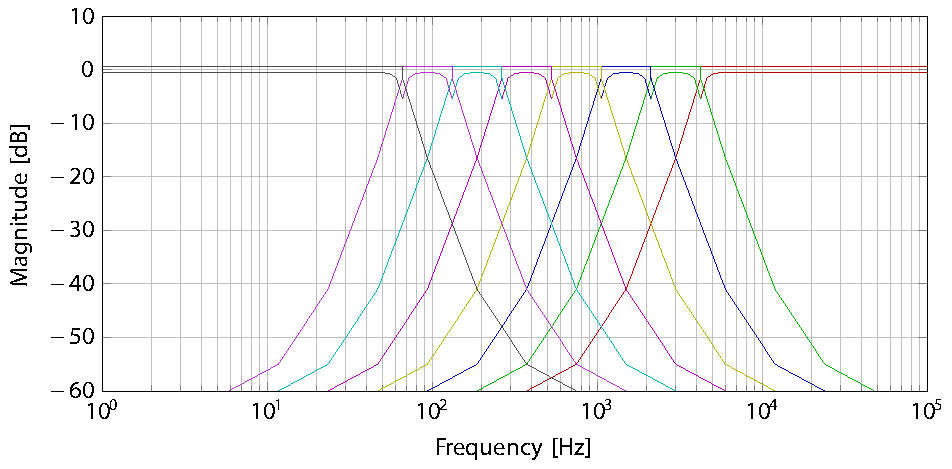
\includegraphics[width=\textwidth]{allBandsExtended}
	\caption{Overview of all band requirements}
	\label{fig:allBands}
\end{figure}
The reason for downsampling seven times and not more or less is because of several reasons. Firstly the bandwidth of the decimation filter must not be influenced by the interpolation filter which would give a non linear frequency response. Therefore every band is set to have a center frequency 1/16 of $f_s$, secondly the lower the center frequency in relation to $f_S$ the higher the filter order and lastly increasing the number of downsamples increases the delay of the system which is not desired in relation to real time applications.      

Because of the reasons the number of stages were based on trial and error, giving the optimal compromise between the just mentioned reasons. If more stages were added, the delay of the system would be to big, and artifacts would occur, while removing additional stages would multiply the filter order by two for every stage removed and giving a user fewer bands in the equalizer.    

Because there will be downsampled by two for every octave band the following relation can be made between a band and $f_S$ as seen on \autoref{fig:relFsBand}.
\begin{figure}[H]
	\centering
	\tikzsetnextfilename{relativeFsBand}
	% This file was created by matlab2tikz.
%
%The latest updates can be retrieved from
%  http://www.mathworks.com/matlabcentral/fileexchange/22022-matlab2tikz-matlab2tikz
%where you can also make suggestions and rate matlab2tikz.
%
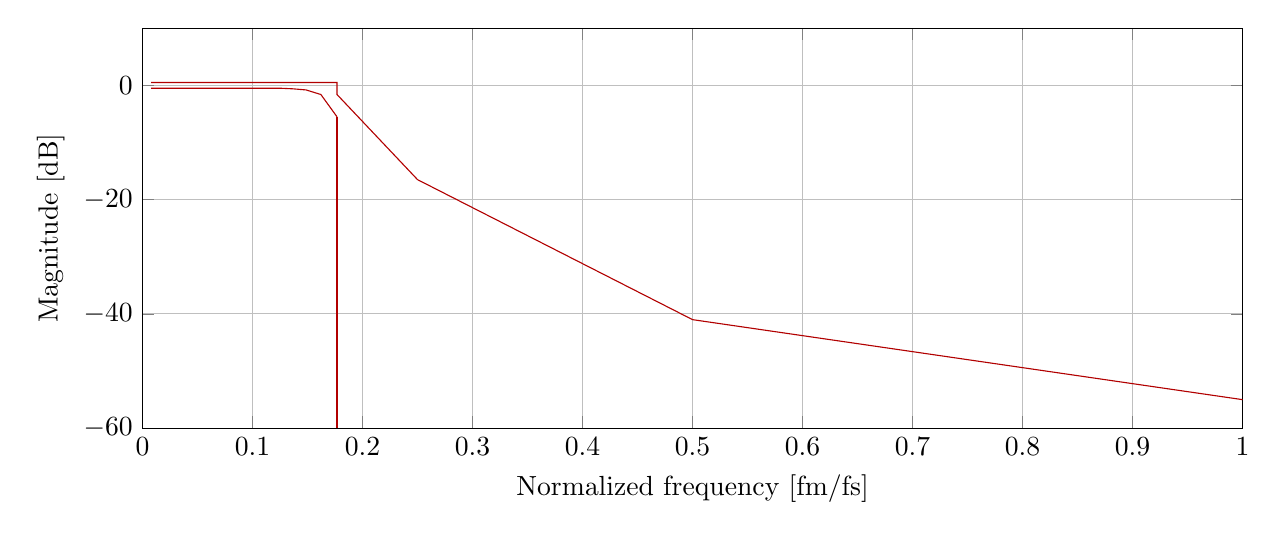
\begin{tikzpicture}

\begin{axis}[%
width=5.5in,
height=2in,
at={(0.758in,0.481in)},
scale only axis,
unbounded coords=jump,
xmin=0,
xmax=1,
xlabel={Normalized frequency [fm/fs]},
xmajorgrids,
ymin=-60,
ymax=10,
ylabel={Magnitude [dB]},
ymajorgrids,
axis background/.style={fill=white}
]
\addplot [color=black!30!red,solid,forget plot]
  table[row sep=crcr]{%
0.1768	-5.5\\
0.1768	-60\\
};
\addplot [color=black!30!red,solid,forget plot]
  table[row sep=crcr]{%
0.0078125	0.5\\
0.015625	0.5\\
0.03125	0.5\\
0.0625	0.5\\
0.0883883476483184	0.5\\
0.0883883476483184	0.5\\
0.0963881765879963	0.5\\
0.105112051906714	0.5\\
0.114625505400584	0.5\\
0.125	0.5\\
0.136313466583157	0.5\\
0.14865088937534	0.5\\
0.162104944331376	0.5\\
0.176776695296637	0.5\\
0.176776695296637	-1.6\\
0.25	-16.5\\
0.5	-41\\
1	-55\\
2	-60\\
};
\addplot [color=black!30!red,solid,forget plot]
  table[row sep=crcr]{%
0.0078125	-0.5\\
0.015625	-0.5\\
0.03125	-0.5\\
0.0625	-0.5\\
0.0883883476483184	-0.5\\
0.0883883476483184	-0.5\\
0.0963881765879963	-0.5\\
0.105112051906714	-0.5\\
0.114625505400584	-0.5\\
0.125	-0.5\\
0.136313466583157	-0.6\\
0.14865088937534	-0.8\\
0.162104944331376	-1.6\\
0.176776695296637	-5.5\\
0.176776695296637	-5.5\\
0.25	-inf\\
0.5	-inf\\
1	-inf\\
2	-inf\\
};
\end{axis}
\end{tikzpicture}%
	\caption{Band relative to $f_s$.}
	\label{fig:relFsBand}
\end{figure}

From \autoref{fig:relFsBand} two points are selected giving the following specifications to the lowpass filter:

$\omega_{pass}=3.000\textrm{ Hz }\cdot 2/f_s=0.1250 \enhed{\pi rad/sample}$\\
$A_{pass}=-1 \enhed{dB}$\\
$\omega_{stop}=6.500\textrm{ Hz }\cdot 2/f_s=0.2708 \enhed{\pi rad/sample}$\\
$A_{stop}=-60 \enhed{dB}$

The design method used for designing the filter is the Kaiser window method, explained in detail in \autoref{app:FIR_theory}. The reason for using the Kaiser window method is that it gives the approximate order of the filter and the beta value of the window applied to impulse reponse. This means that no trial and error method is needed to meet the requirements for the filter.

With the specification stated and using the FIR theoy explained in \autoref{app:FIR_theory} about the Kaiser window method and deriving the coefficients of the filter, the following filter is given with quantisized coefficients, see \autoref{fig:band1_filt} for magnitude response and \autoref{fig:band1_filtPhase} for phase response. The order of the filter is 50, it is a type 1 FIR filter and has linear phase which means that the group delay is constant at 25 samples.  

\begin{figure}[H]
\centering
	\tikzsetnextfilename{Band1Filt}
	% This file was created by matlab2tikz.
%
%The latest updates can be retrieved from
%  http://www.mathworks.com/matlabcentral/fileexchange/22022-matlab2tikz-matlab2tikz
%where you can also make suggestions and rate matlab2tikz.
%
\definecolor{mycolor1}{rgb}{0.00000,0.44700,0.74100}%
%
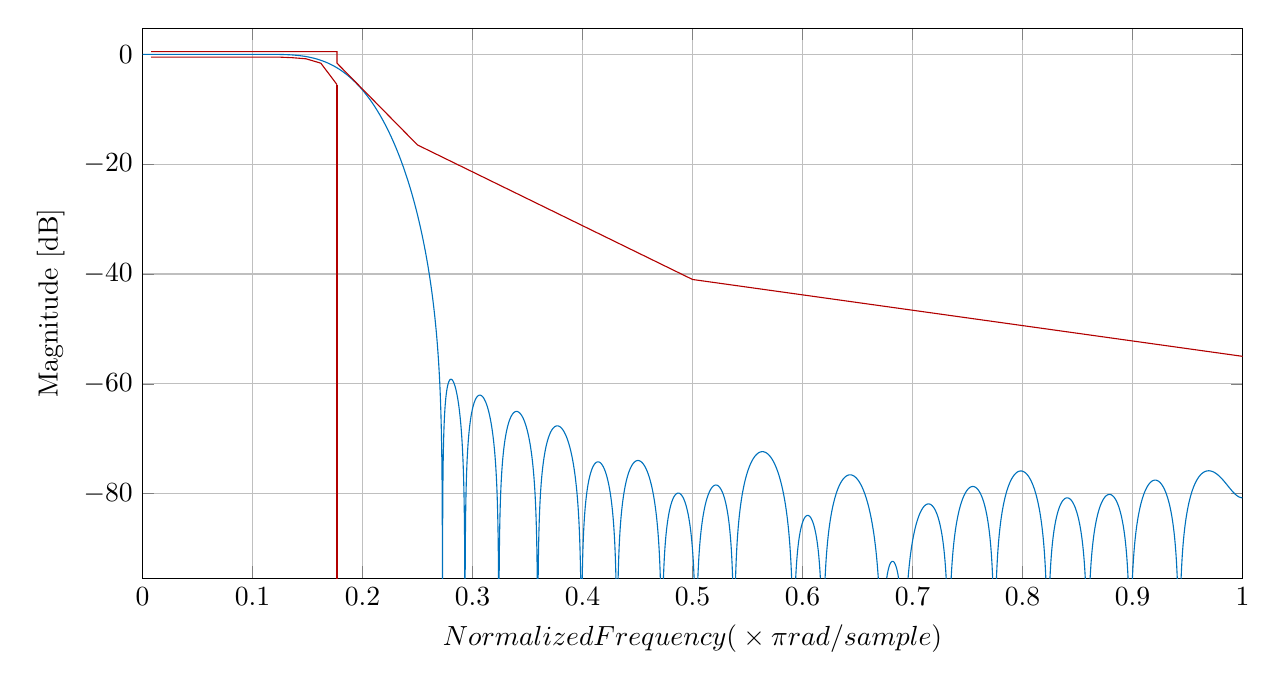
\begin{tikzpicture}

\begin{axis}[%
width=5.5in,
height=2.75in,
at={(1.281in,0.447in)},
scale only axis,
unbounded coords=jump,
xmin=0,
xmax=1,
xlabel={$\text{Normalized Frequency (}\times\pi\text{ rad/sample)}$},
xmajorgrids,
ymin=-95.4207080394785,
ymax=4.7713185812425,
ylabel={Magnitude [dB]},
ymajorgrids,
axis background/.style={fill=white},
]
\addplot [color=mycolor1,solid,forget plot]
  table[row sep=crcr]{%
0	0.002385323281203\\
0.0001220703125	0.00238515620543467\\
0.000244140625	0.00238465500069651\\
0.0003662109375	0.00238381973514379\\
0.00048828125	0.00238265052200859\\
0.0006103515625	0.00238114752011143\\
0.000732421875	0.00237931093340649\\
0.0008544921875	0.00237714101120901\\
0.0009765625	0.00237463804796789\\
0.0010986328125	0.00237180238360679\\
0.001220703125	0.00236863440289881\\
0.0013427734375	0.00236513453592124\\
0.00146484375	0.00236130325782824\\
0.0015869140625	0.00235714108868024\\
0.001708984375	0.00235264859355766\\
0.0018310546875	0.00234782638233355\\
0.001953125	0.00234267510978725\\
0.0020751953125	0.0023371954752065\\
0.002197265625	0.00233138822267165\\
0.0023193359375	0.00232525414077145\\
0.00244140625	0.00231879406231883\\
0.0025634765625	0.00231200886469196\\
0.002685546875	0.00230489946932266\\
0.0028076171875	0.00229746684169641\\
0.0029296875	0.00228971199135231\\
0.0030517578125	0.00228163597159892\\
0.003173828125	0.00227323987945738\\
0.0032958984375	0.00226452485554773\\
0.00341796875	0.00225549208369102\\
0.0035400390625	0.00224614279125035\\
0.003662109375	0.00223647824844875\\
0.0037841796875	0.00222649976865341\\
0.00390625	0.00221620870775041\\
0.0040283203125	0.00220560646437207\\
0.004150390625	0.00219469447961274\\
0.0042724609375	0.0021834742366309\\
0.00439453125	0.00217194726076286\\
0.0045166015625	0.002160115119068\\
0.004638671875	0.00214797942038558\\
0.0047607421875	0.00213554181482323\\
0.0048828125	0.0021228039938137\\
0.0050048828125	0.00210976768977389\\
0.005126953125	0.00209643467593423\\
0.0052490234375	0.00208280676594086\\
0.00537109375	0.00206888581396925\\
0.0054931640625	0.00205467371409895\\
0.005615234375	0.00204017240037047\\
0.0057373046875	0.0020253838462736\\
0.005859375	0.00201031006480434\\
0.0059814453125	0.00199495310783959\\
0.006103515625	0.00197931506625082\\
0.0062255859375	0.0019633980693925\\
0.00634765625	0.00194720428476103\\
0.0064697265625	0.00193073591810844\\
0.006591796875	0.00191399521258973\\
0.0067138671875	0.00189698444904707\\
0.0068359375	0.00187970594521403\\
0.0069580078125	0.00186216205582923\\
0.007080078125	0.00184435517201109\\
0.0072021484375	0.00182628772120097\\
0.00732421875	0.00180796216670842\\
0.0074462890625	0.0017893810073133\\
0.007568359375	0.00177054677726574\\
0.0076904296875	0.00175146204554721\\
0.0078125	0.00173212941587053\\
0.0079345703125	0.00171255152616823\\
0.008056640625	0.00169273104819467\\
0.0081787109375	0.00167267068746924\\
0.00830078125	0.0016523731825373\\
0.0084228515625	0.00163184130502714\\
0.008544921875	0.0016110778589109\\
0.0086669921875	0.00159008568039098\\
0.0087890625	0.00156886763744524\\
0.0089111328125	0.00154742662942908\\
0.009033203125	0.00152576558673445\\
0.0091552734375	0.00150388747044872\\
0.00927734375	0.00148179527189996\\
0.0093994140625	0.00145949201237272\\
0.009521484375	0.00143698074248277\\
0.0096435546875	0.00141426454212024\\
0.009765625	0.00139134651976747\\
0.0098876953125	0.00136822981221485\\
0.010009765625	0.00134491758416289\\
0.0101318359375	0.00132141302776745\\
0.01025390625	0.00129771936218503\\
0.0103759765625	0.00127383983328855\\
0.010498046875	0.00124977771315571\\
0.0106201171875	0.00122553629967115\\
0.0107421875	0.00120111891595798\\
0.0108642578125	0.0011765289102641\\
0.010986328125	0.00115176965510955\\
0.0111083984375	0.00112684454722967\\
0.01123046875	0.00110175700689297\\
0.0113525390625	0.00107651047756008\\
0.011474609375	0.00105110842537215\\
0.0115966796875	0.00102555433869611\\
0.01171875	0.000999851727783607\\
0.0118408203125	0.000974004124145722\\
0.011962890625	0.000948015080211917\\
0.0120849609375	0.000921888168818441\\
0.01220703125	0.000895626982753583\\
0.0123291015625	0.000869235134302926\\
0.012451171875	0.000842716254624065\\
0.0125732421875	0.000816073993576083\\
0.0126953125	0.000789312018923738\\
0.0128173828125	0.000762434016110092\\
0.012939453125	0.000735443687460702\\
0.0130615234375	0.000708344752126777\\
0.01318359375	0.000681140945175684\\
0.0133056640625	0.000653836017420417\\
0.013427734375	0.000626433734680631\\
0.0135498046875	0.000598937877441585\\
0.013671875	0.000571352240285705\\
0.0137939453125	0.000543680631437837\\
0.013916015625	0.000515926872139971\\
0.0140380859375	0.000488094796423866\\
0.01416015625	0.000460188250258398\\
0.0142822265625	0.000432211091322188\\
0.014404296875	0.000404167188264637\\
0.0145263671875	0.000376060420308022\\
0.0146484375	0.000347894676849592\\
0.0147705078125	0.000319673856722602\\
0.014892578125	0.000291401867798413\\
0.0150146484375	0.000263082626418054\\
0.01513671875	0.00023472005699432\\
0.0152587890625	0.000206318091272806\\
0.015380859375	0.000177880668047692\\
0.0155029296875	0.000149411732422777\\
0.015625	0.000120915235413577\\
0.0157470703125	9.23951334357298e-05\\
0.015869140625	6.38553876228798e-05\\
0.0159912109375	3.52999635424567e-05\\
0.01611328125	6.73283045671269e-06\\
0.0162353515625	-2.18420391888685e-05\\
0.016357421875	-5.04206701634757e-05\\
0.0164794921875	-7.89990851330913e-05\\
0.0166015625	-0.000107573305172082\\
0.0167236328125	-0.000136139350047415\\
0.016845703125	-0.000164693239241842\\
0.0169677734375	-0.00019323099201074\\
0.01708984375	-0.000221748628234764\\
0.0172119140625	-0.000250242168704062\\
0.017333984375	-0.000278707636027775\\
0.0174560546875	-0.000307141054690874\\
0.017578125	-0.000335538451963657\\
0.0177001953125	-0.000363895858299657\\
0.017822265625	-0.000392209307847224\\
0.0179443359375	-0.000420474839074814\\
0.01806640625	-0.000448688495225724\\
0.0181884765625	-0.000476846324943381\\
0.018310546875	-0.00050494438272608\\
0.0184326171875	-0.000532978729438582\\
0.0185546875	-0.000560945432937388\\
0.0186767578125	-0.000588840568696014\\
0.018798828125	-0.000616660220032372\\
0.0189208984375	-0.000644400478904572\\
0.01904296875	-0.000672057446479357\\
0.0191650390625	-0.000699627233359479\\
0.019287109375	-0.000727105960436347\\
0.0194091796875	-0.000754489759344779\\
0.01953125	-0.000781774772860899\\
0.0196533203125	-0.00080895715564111\\
0.019775390625	-0.00083603307444946\\
0.0198974609375	-0.000862998709010299\\
0.02001953125	-0.00088985025246302\\
0.0201416015625	-0.000916583911646285\\
0.020263671875	-0.00094319590800751\\
0.0203857421875	-0.00096968247771656\\
0.0205078125	-0.000996039872518395\\
0.0206298828125	-0.00102226436018782\\
0.020751953125	-0.0010483522248137\\
0.0208740234375	-0.00107429976765161\\
0.02099609375	-0.00110010330740806\\
0.0211181640625	-0.00112575918086577\\
0.021240234375	-0.00115126374339525\\
0.0213623046875	-0.00117661336929586\\
0.021484375	-0.0012018044526485\\
0.0216064453125	-0.00122683340742924\\
0.021728515625	-0.00125169666830516\\
0.0218505859375	-0.00127639069108909\\
0.02197265625	-0.001300911952967\\
0.0220947265625	-0.00132525695352115\\
0.022216796875	-0.00134942221467327\\
0.0223388671875	-0.00137340428153721\\
0.0224609375	-0.00139719972275998\\
0.0225830078125	-0.00142080513114706\\
0.022705078125	-0.0014442171239466\\
0.0228271484375	-0.00146743234347468\\
0.02294921875	-0.0014904474575701\\
0.0230712890625	-0.00151325916010592\\
0.023193359375	-0.00153586417133056\\
0.0233154296875	-0.00155825923854991\\
0.0234375	-0.00158044113641154\\
0.0235595703125	-0.00160240666741629\\
0.023681640625	-0.00162415266248672\\
0.0238037109375	-0.001645675981365\\
0.02392578125	-0.00166697351295397\\
0.0240478515625	-0.00168804217588558\\
0.024169921875	-0.00170887891908933\\
0.0242919921875	-0.00172948072201962\\
0.0244140625	-0.00174984459516736\\
0.0245361328125	-0.00176996758062842\\
0.024658203125	-0.00178984675221727\\
0.0247802734375	-0.00180947921643337\\
0.02490234375	-0.00182886211234745\\
0.0250244140625	-0.00184799261228363\\
0.025146484375	-0.00186686792238788\\
0.0252685546875	-0.001885485282628\\
0.025390625	-0.0019038419677031\\
0.0255126953125	-0.00192193528698681\\
0.025634765625	-0.00193976258526618\\
0.0257568359375	-0.00195732124313963\\
0.02587890625	-0.00197460867707377\\
0.0260009765625	-0.00199162234019923\\
0.026123046875	-0.00200835972248115\\
0.0262451171875	-0.00202481835128765\\
0.0263671875	-0.00204099579133299\\
0.0264892578125	-0.00205688964575756\\
0.026611328125	-0.00207249755578687\\
0.0267333984375	-0.00208781720164097\\
0.02685546875	-0.00210284630253454\\
0.0269775390625	-0.00211758261724526\\
0.027099609375	-0.00213202394439804\\
0.0272216796875	-0.0021461681228061\\
0.02734375	-0.00216001303186886\\
0.0274658203125	-0.00217355659185614\\
0.027587890625	-0.00218679676419242\\
0.0277099609375	-0.00219973155202524\\
0.02783203125	-0.00221235900016836\\
0.0279541015625	-0.00222467719572705\\
0.028076171875	-0.00223668426843915\\
0.0281982421875	-0.00224837839073189\\
0.0283203125	-0.00225975777811982\\
0.0284423828125	-0.0022708206897164\\
0.028564453125	-0.00228156542817715\\
0.0286865234375	-0.0022919903403249\\
0.02880859375	-0.0023020938172067\\
0.0289306640625	-0.0023118742944348\\
0.029052734375	-0.00232133025252779\\
0.0291748046875	-0.00233046021702421\\
0.029296875	-0.00233926275899421\\
0.0294189453125	-0.0023477364950395\\
0.029541015625	-0.00235588008769128\\
0.0296630859375	-0.00236369224552391\\
0.02978515625	-0.00237117172355283\\
0.0299072265625	-0.00237831732351879\\
0.030029296875	-0.0023851278937741\\
0.0301513671875	-0.00239160232990798\\
0.0302734375	-0.00239773957468969\\
0.0303955078125	-0.00240353861840958\\
0.030517578125	-0.00240899849904963\\
0.0306396484375	-0.00241411830245397\\
0.03076171875	-0.00241889716261312\\
0.0308837890625	-0.00242333426177765\\
0.031005859375	-0.0024274288305719\\
0.0311279296875	-0.00243118014827814\\
0.03125	-0.00243458754306403\\
0.0313720703125	-0.00243765039192567\\
0.031494140625	-0.00244036812108561\\
0.0316162109375	-0.00244274020593593\\
0.03173828125	-0.00244476617137934\\
0.0318603515625	-0.00244644559177232\\
0.031982421875	-0.00244777809115249\\
0.0321044921875	-0.002448763343466\\
0.0322265625	-0.00244940107251068\\
0.0323486328125	-0.00244969105204973\\
0.032470703125	-0.00244963310615276\\
0.0325927734375	-0.00244922710896844\\
0.03271484375	-0.00244847298506556\\
0.0328369140625	-0.00244737070943302\\
0.032958984375	-0.00244592030753665\\
0.0330810546875	-0.00244412185537612\\
0.033203125	-0.0024419754797691\\
0.0333251953125	-0.00243948135795335\\
0.033447265625	-0.00243663971821206\\
0.0335693359375	-0.00243345083941904\\
0.03369140625	-0.00242991505143664\\
0.0338134765625	-0.00242603273483155\\
0.033935546875	-0.00242180432132955\\
0.0340576171875	-0.00241723029330387\\
0.0341796875	-0.00241231118434371\\
0.0343017578125	-0.00240704757874255\\
0.034423828125	-0.00240144011183929\\
0.0345458984375	-0.00239548947007506\\
0.03466796875	-0.00238919639048163\\
0.0347900390625	-0.00238256166136352\\
0.034912109375	-0.00237558612161592\\
0.0350341796875	-0.00236827066112255\\
0.03515625	-0.00236061622064199\\
0.0352783203125	-0.0023526237915803\\
0.035400390625	-0.00234429441604789\\
0.0355224609375	-0.00233562918691632\\
0.03564453125	-0.00232662924753413\\
0.0357666015625	-0.00231729579178364\\
0.035888671875	-0.00230763006408097\\
0.0360107421875	-0.00229763335897815\\
0.0361328125	-0.00228730702150415\\
0.0362548828125	-0.00227665244659647\\
0.036376953125	-0.00226567107949904\\
0.0364990234375	-0.00225436441508009\\
0.03662109375	-0.00224273399823005\\
0.0367431640625	-0.00223078142346367\\
0.036865234375	-0.00221850833469261\\
0.0369873046875	-0.00220591642545287\\
0.037109375	-0.00219300743833628\\
0.0372314453125	-0.00217978316510425\\
0.037353515625	-0.00216624544640354\\
0.0374755859375	-0.00215239617165253\\
0.03759765625	-0.00213823727892759\\
0.0377197265625	-0.00212377075445147\\
0.037841796875	-0.00210899863299119\\
0.0379638671875	-0.00209392299706224\\
0.0380859375	-0.00207854597704227\\
0.0382080078125	-0.00206286975094372\\
0.038330078125	-0.0020468965441296\\
0.0384521484375	-0.00203062862914294\\
0.03857421875	-0.00201406832536577\\
0.0386962890625	-0.0019972179989054\\
0.038818359375	-0.00198008006236705\\
0.0389404296875	-0.00196265697445597\\
0.0390625	-0.00194495123980687\\
0.0391845703125	-0.00192696540869974\\
0.039306640625	-0.00190870207694616\\
0.0394287109375	-0.00189016388526397\\
0.03955078125	-0.00187135351933421\\
0.0396728515625	-0.00185227370934626\\
0.039794921875	-0.00183292722977058\\
0.0399169921875	-0.00181331689884701\\
0.0400390625	-0.00179344557864169\\
0.0401611328125	-0.00177331617442178\\
0.040283203125	-0.00175293163448487\\
0.0404052734375	-0.00173229494964744\\
0.04052734375	-0.00171140915324486\\
0.0406494140625	-0.00169027732044924\\
0.040771484375	-0.00166890256804209\\
0.0408935546875	-0.00164728805413006\\
0.041015625	-0.00162543697774709\\
0.0411376953125	-0.00160335257839961\\
0.041259765625	-0.00158103813578236\\
0.0413818359375	-0.00155849696932364\\
0.04150390625	-0.0015357324379579\\
0.0416259765625	-0.00151274793944367\\
0.041748046875	-0.00148954691024983\\
0.0418701171875	-0.00146613282504404\\
0.0419921875	-0.00144250919629485\\
0.0421142578125	-0.00141867957364639\\
0.042236328125	-0.00139464754391838\\
0.0423583984375	-0.00137041673031035\\
0.04248046875	-0.00134599079211739\\
0.0426025390625	-0.00132137342427541\\
0.042724609375	-0.00129656835684955\\
0.0428466796875	-0.00127157935469313\\
0.04296875	-0.00124641021693606\\
0.0430908203125	-0.00122106477641637\\
0.043212890625	-0.00119554689933921\\
0.0433349609375	-0.00116986048493573\\
0.04345703125	-0.00114400946455362\\
0.0435791015625	-0.00111799780154342\\
0.043701171875	-0.00109182949069009\\
0.0438232421875	-0.00106550855758769\\
0.0439453125	-0.00103903905829839\\
0.0440673828125	-0.00101242507867028\\
0.044189453125	-0.000985670733996358\\
0.0443115234375	-0.000958780168389239\\
0.04443359375	-0.000931757554269552\\
0.0445556640625	-0.000904607091854359\\
0.044677734375	-0.000877333008645564\\
0.0447998046875	-0.000849939558804635\\
0.044921875	-0.000822431022641013\\
0.0450439453125	-0.000794811706214205\\
0.045166015625	-0.000767085940424295\\
0.0452880859375	-0.000739258080955096\\
0.04541015625	-0.000711332507080442\\
0.0455322265625	-0.00068331362177787\\
0.045654296875	-0.000655205850591756\\
0.0457763671875	-0.000627013641349095\\
0.0458984375	-0.000598741463477381\\
0.0460205078125	-0.000570393807493019\\
0.046142578125	-0.000541975184319199\\
0.0462646484375	-0.000513490124717464\\
0.04638671875	-0.000484943178662434\\
0.0465087890625	-0.000456338914830212\\
0.046630859375	-0.000427681919916267\\
0.0467529296875	-0.000398976798010153\\
0.046875	-0.000370228170027076\\
0.0469970703125	-0.000341440672968929\\
0.047119140625	-0.000312618959469546\\
0.0472412109375	-0.000283767696998893\\
0.04736328125	-0.000254891567465165\\
0.0474853515625	-0.000225995266191603\\
0.047607421875	-0.000197083501632278\\
0.0477294921875	-0.000168160994633126\\
0.0478515625	-0.000139232477636142\\
0.0479736328125	-0.000110302694281472\\
0.048095703125	-8.13763983842364e-05\\
0.0482177734375	-5.24583537071521e-05\\
0.04833984375	-2.35533330510407e-05\\
0.0484619140625	5.33388254098099e-06\\
0.048583984375	3.41985040677173e-05\\
0.0487060546875	6.30357355930755e-05\\
0.048828125	9.18407747576566e-05\\
0.0489501953125	0.000120608813460876\\
0.049072265625	0.000149335038599929\\
0.0491943359375	0.000178014632695067\\
0.04931640625	0.000206642774685406\\
0.0494384765625	0.000235214640440518\\
0.049560546875	0.000263725403556236\\
0.0496826171875	0.000292170236036782\\
0.0498046875	0.000320544309147408\\
0.0499267578125	0.000348842793698623\\
0.050048828125	0.000377060861239897\\
0.0501708984375	0.000405193684400729\\
0.05029296875	0.000433236437800133\\
0.0504150390625	0.000461184298558237\\
0.050537109375	0.00048903244731946\\
0.0506591796875	0.000516776068593572\\
0.05078125	0.000544410351835722\\
0.0509033203125	0.000571930491730654\\
0.051025390625	0.000599331689386418\\
0.0511474609375	0.000626609152618585\\
0.05126953125	0.00065375809708712\\
0.0513916015625	0.000680773746580599\\
0.051513671875	0.000707651334039383\\
0.0516357421875	0.000734386102294593\\
0.0517578125	0.00076097330452285\\
0.0518798828125	0.000787408205326301\\
0.052001953125	0.00081368608101684\\
0.0521240234375	0.000839802220866659\\
0.05224609375	0.000865751927392466\\
0.0523681640625	0.000891530517378669\\
0.052490234375	0.00091713332233212\\
0.0526123046875	0.000942555689618985\\
0.052734375	0.000967792982635274\\
0.0528564453125	0.000992840582057397\\
0.052978515625	0.00101769388629691\\
0.0531005859375	0.00104234831229633\\
0.05322265625	0.00106679929626807\\
0.0533447265625	0.00109104229443346\\
0.053466796875	0.00111507278364797\\
0.0535888671875	0.00113888626236758\\
0.0537109375	0.00116247825098981\\
0.0538330078125	0.00118584429316115\\
0.053955078125	0.00120897995577707\\
0.0540771484375	0.00123188083051673\\
0.05419921875	0.00125454253378621\\
0.0543212890625	0.00127696070802585\\
0.054443359375	0.00129913102216506\\
0.0545654296875	0.00132104917247489\\
0.0546875	0.00134271088313653\\
0.0548095703125	0.0013641119071508\\
0.054931640625	0.00138524802679285\\
0.0550537109375	0.00140611505469224\\
0.05517578125	0.00142670883428764\\
0.0552978515625	0.00144702524062268\\
0.055419921875	0.00146706018114173\\
0.0555419921875	0.00148680959614467\\
0.0556640625	0.00150626945986687\\
0.0557861328125	0.00152543578087716\\
0.055908203125	0.00154430460304411\\
0.0560302734375	0.00156287200599081\\
0.05615234375	0.00158113410600436\\
0.0562744140625	0.00159908705660428\\
0.056396484375	0.00161672704928151\\
0.0565185546875	0.00163405031435104\\
0.056640625	0.00165105312134983\\
0.0567626953125	0.00166773177994628\\
0.056884765625	0.00168408264056552\\
0.0570068359375	0.00170010209512839\\
0.05712890625	0.00171578657767668\\
0.0572509765625	0.00173113256499846\\
0.057373046875	0.00174613657748068\\
0.0574951171875	0.00176079517967764\\
0.0576171875	0.00177510498087941\\
0.0577392578125	0.00178906263596446\\
0.057861328125	0.00180266484602498\\
0.0579833984375	0.00181590835899215\\
0.05810546875	0.00182878997020453\\
0.0582275390625	0.00184130652326076\\
0.058349609375	0.00185345491053113\\
0.0584716796875	0.00186523207378286\\
0.05859375	0.00187663500503277\\
0.0587158203125	0.0018876607467746\\
0.058837890625	0.00189830639317279\\
0.0589599609375	0.00190856909023296\\
0.05908203125	0.00191844603648406\\
0.0592041015625	0.00192793448394468\\
0.059326171875	0.00193703173829363\\
0.0594482421875	0.00194573515977936\\
0.0595703125	0.00195404216373163\\
0.0596923828125	0.00196195022118673\\
0.059814453125	0.00196945685939909\\
0.0599365234375	0.00197655966246657\\
0.06005859375	0.00198325627212625\\
0.0601806640625	0.00198954438798182\\
0.060302734375	0.00199542176835621\\
0.0604248046875	0.0020008862306895\\
0.060546875	0.00200593565227791\\
0.0606689453125	0.00201056797067167\\
0.060791015625	0.00201478118435716\\
0.0609130859375	0.00201857335315481\\
0.06103515625	0.00202194259884436\\
0.0611572265625	0.00202488710584703\\
0.061279296875	0.00202740512150967\\
0.0614013671875	0.00202949495678695\\
0.0615234375	0.00203115498663919\\
0.0616455078125	0.00203238365065772\\
0.061767578125	0.00203317945351955\\
0.0618896484375	0.00203354096555586\\
0.06201171875	0.00203346682309302\\
0.0621337890625	0.00203295572913476\\
0.062255859375	0.00203200645358947\\
0.0623779296875	0.00203061783400926\\
0.0625	0.00202878877593093\\
0.0626220703125	0.00202651825327393\\
0.062744140625	0.00202380530885193\\
0.0628662109375	0.00202064905494126\\
0.06298828125	0.00201704867345143\\
0.0631103515625	0.00201300341655042\\
0.063232421875	0.00200851260700574\\
0.0633544921875	0.00200357563875286\\
0.0634765625	0.00199819197706574\\
0.0635986328125	0.00199236115901158\\
0.063720703125	0.00198608279401924\\
0.0638427734375	0.00197935656410664\\
0.06396484375	0.00197218222416495\\
0.0640869140625	0.00196455960264075\\
0.064208984375	0.00195648860153597\\
0.0643310546875	0.00194796919709006\\
0.064453125	0.00193900143972314\\
0.0645751953125	0.00192958545477495\\
0.064697265625	0.00191972144267538\\
0.0648193359375	0.00190940967911502\\
0.06494140625	0.00189865051549987\\
0.0650634765625	0.00188744437934929\\
0.065185546875	0.00187579177429598\\
0.0653076171875	0.00186369328065439\\
0.0654296875	0.00185114955553445\\
0.0655517578125	0.00183816133312575\\
0.065673828125	0.00182472942503864\\
0.0657958984375	0.00181085472036102\\
0.06591796875	0.00179653818616998\\
0.0660400390625	0.00178178086741809\\
0.066162109375	0.00176658388744499\\
0.0662841796875	0.00175094844803425\\
0.06640625	0.00173487582969756\\
0.0665283203125	0.00171836739173159\\
0.066650390625	0.00170142457255906\\
0.0667724609375	0.00168404888978557\\
0.06689453125	0.00166624194025644\\
0.0670166015625	0.00164800540056831\\
0.067138671875	0.00162934102678491\\
0.0672607421875	0.001610250654835\\
0.0673828125	0.00159073620051231\\
0.0675048828125	0.00157079965964613\\
0.067626953125	0.00155044310815811\\
0.0677490234375	0.00152966870211912\\
0.06787109375	0.00150847867797665\\
0.0679931640625	0.00148687535238423\\
0.068115234375	0.00146486112248567\\
0.0682373046875	0.00144243846574454\\
0.068359375	0.00141960994017154\\
0.0684814453125	0.00139637818426763\\
0.068603515625	0.00137274591702408\\
0.0687255859375	0.00134871593786556\\
0.06884765625	0.00132429112682075\\
0.0689697265625	0.00129947444435174\\
0.069091796875	0.00127426893124039\\
0.0692138671875	0.00124867770887249\\
0.0693359375	0.0012227039787831\\
0.0694580078125	0.00119635102288385\\
0.069580078125	0.00116962220323558\\
0.0697021484375	0.00114252096210521\\
0.06982421875	0.00111505082162466\\
0.0699462890625	0.00108721538390455\\
0.070068359375	0.00105901833080679\\
0.0701904296875	0.0010304634238878\\
0.0703125	0.00100155450411421\\
0.0704345703125	0.000972295491806108\\
0.070556640625	0.000942690386523282\\
0.0706787109375	0.000912743266667349\\
0.07080078125	0.000882458289595434\\
0.0709228515625	0.00085183969110858\\
0.071044921875	0.000820891785451749\\
0.0711669921875	0.00078961896497276\\
0.0712890625	0.000758025699894915\\
0.0714111328125	0.000726116538203314\\
0.071533203125	0.000693896105076419\\
0.0716552734375	0.000661369102886056\\
0.07177734375	0.000628540310856351\\
0.0718994140625	0.000595414584665832\\
0.072021484375	0.000561996856163205\\
0.0721435546875	0.000528292133026298\\
0.072265625	0.00049430549859153\\
0.0723876953125	0.000460042111228631\\
0.072509765625	0.000425507204170117\\
0.0726318359375	0.000390706085056536\\
0.07275390625	0.000355644135595412\\
0.0728759765625	0.000320326811163341\\
0.072998046875	0.000284759640237553\\
0.0731201171875	0.000248948224225387\\
0.0732421875	0.000212898236725323\\
0.0733642578125	0.000176615423470139\\
0.073486328125	0.000140105601417417\\
0.0736083984375	0.000103374658579014\\
0.07373046875	6.64285533957809e-05\\
0.0738525390625	2.92733142828183e-05\\
0.073974609375	-8.08496088211541e-06\\
0.0740966796875	-4.56401052701949e-05\\
0.07421875	-8.33858838404922e-05\\
0.0743408203125	-0.000121315993510507\\
0.074462890625	-0.000159424064122504\\
0.0745849609375	-0.000197703658841419\\
0.07470703125	-0.000236148274609604\\
0.0748291015625	-0.000274751343056323\\
0.074951171875	-0.000313506230952498\\
0.0750732421875	-0.000352406240779146\\
0.0751953125	-0.000391444611466341\\
0.0753173828125	-0.000430614519132178\\
0.075439453125	-0.000469909077594366\\
0.0755615234375	-0.000509321339052349\\
0.07568359375	-0.000548844295053641\\
0.0758056640625	-0.000588470876778047\\
0.075927734375	-0.000628193956117684\\
0.0760498046875	-0.000668006346359107\\
0.076171875	-0.000707900802694894\\
0.0762939453125	-0.000747870023303676\\
0.076416015625	-0.000787906649861725\\
0.0765380859375	-0.000828003268622979\\
0.07666015625	-0.000868152410930634\\
0.0767822265625	-0.000908346554126638\\
0.076904296875	-0.000948578122518029\\
0.0770263671875	-0.000988839488059057\\
0.0771484375	-0.00102912297126068\\
0.0772705078125	-0.0010694208420432\\
0.077392578125	-0.00110972532075948\\
0.0775146484375	-0.00115002857882018\\
0.07763671875	-0.00119032273977382\\
0.0777587890625	-0.00123059988032992\\
0.077880859375	-0.00127085203104116\\
0.0780029296875	-0.00131107117738338\\
0.078125	-0.00135124926077879\\
0.0782470703125	-0.00139137817944857\\
0.078369140625	-0.00143144978949294\\
0.0784912109375	-0.00147145590585751\\
0.07861328125	-0.0015113883033564\\
0.0787353515625	-0.00155123871752494\\
0.078857421875	-0.00159099884609759\\
0.0789794921875	-0.00163066034951953\\
0.0791015625	-0.00167021485236774\\
0.0792236328125	-0.00170965394437417\\
0.079345703125	-0.00174896918139211\\
0.0794677734375	-0.00178815208670358\\
0.07958984375	-0.00182719415187194\\
0.0797119140625	-0.00186608683804934\\
0.079833984375	-0.00190482157717042\\
0.0799560546875	-0.00194338977286179\\
0.080078125	-0.00198178280186312\\
0.0802001953125	-0.00201999201510716\\
0.080322265625	-0.00205800873891349\\
0.0804443359375	-0.00209582427612531\\
0.08056640625	-0.00213342990741694\\
0.0806884765625	-0.00217081689254428\\
0.080810546875	-0.00220797647153859\\
0.0809326171875	-0.00224489986584331\\
0.0810546875	-0.00228157827979203\\
0.0811767578125	-0.00231800290191586\\
0.081298828125	-0.00235416490585294\\
0.0814208984375	-0.00239005545216742\\
0.08154296875	-0.00242566568914526\\
0.0816650390625	-0.00246098675472695\\
0.081787109375	-0.00249600977713271\\
0.0819091796875	-0.00253072587696579\\
0.08203125	-0.00256512616783766\\
0.0821533203125	-0.00259920175841444\\
0.082275390625	-0.00263294375332634\\
0.0823974609375	-0.00266634325481618\\
0.08251953125	-0.00269939136398989\\
0.0826416015625	-0.00273207918240814\\
0.082763671875	-0.00276439781345061\\
0.0828857421875	-0.00279633836362336\\
0.0830078125	-0.00282789194426414\\
0.0831298828125	-0.00285904967284978\\
0.083251953125	-0.00288980267453098\\
0.0833740234375	-0.0029201420835534\\
0.08349609375	-0.00295005904484924\\
0.0836181640625	-0.00297954471562889\\
0.083740234375	-0.00300859026663147\\
0.0838623046875	-0.00303718688388699\\
0.083984375	-0.00306532577019425\\
0.0841064453125	-0.00309299814676933\\
0.084228515625	-0.00312019525466667\\
0.0843505859375	-0.00314690835637066\\
0.08447265625	-0.00317312873755782\\
0.0845947265625	-0.00319884770851786\\
0.084716796875	-0.003224056605859\\
0.0848388671875	-0.00324874679409959\\
0.0849609375	-0.00327290966720284\\
0.0850830078125	-0.00329653665045271\\
0.085205078125	-0.0033196192019318\\
0.0853271484375	-0.00334214881422668\\
0.08544921875	-0.00336411701607631\\
0.0855712890625	-0.00338551537407739\\
0.085693359375	-0.00340633549444647\\
0.0858154296875	-0.00342656902449789\\
0.0859375	-0.00344620765469017\\
0.0860595703125	-0.00346524312004703\\
0.086181640625	-0.00348366720209015\\
0.0863037109375	-0.00350147173048754\\
0.08642578125	-0.00351864858464523\\
0.0865478515625	-0.00353518969592415\\
0.086669921875	-0.00355108704889062\\
0.0867919921875	-0.00356633268341966\\
0.0869140625	-0.00358091869634336\\
0.0870361328125	-0.00359483724326992\\
0.087158203125	-0.00360808054051631\\
0.0872802734375	-0.00362064086664304\\
0.08740234375	-0.00363251056455738\\
0.0875244140625	-0.00364368204310495\\
0.087646484375	-0.0036541477791161\\
0.0877685546875	-0.00366390031905439\\
0.087890625	-0.00367293228111976\\
0.0880126953125	-0.00368123635672646\\
0.088134765625	-0.00368880531289051\\
0.0882568359375	-0.00369563199348022\\
0.08837890625	-0.00370170932177416\\
0.0885009765625	-0.00370703030171171\\
0.088623046875	-0.00371158802028049\\
0.0887451171875	-0.0037153756491648\\
0.0888671875	-0.00371838644673517\\
0.0889892578125	-0.00372061375998101\\
0.089111328125	-0.00372205102627277\\
0.0892333984375	-0.00372269177557882\\
0.08935546875	-0.00372252963228448\\
0.0894775390625	-0.00372155831695409\\
0.089599609375	-0.00371977164854798\\
0.0897216796875	-0.00371716354618457\\
0.08984375	-0.00371372803135728\\
0.0899658203125	-0.00370945922952615\\
0.090087890625	-0.0037043513724484\\
0.0902099609375	-0.00369839879994061\\
0.09033203125	-0.00369159596198188\\
0.0904541015625	-0.00368393742064654\\
0.090576171875	-0.00367541785203684\\
0.0906982421875	-0.00366603204861349\\
0.0908203125	-0.00365577492061675\\
0.0909423828125	-0.00364464149868127\\
0.091064453125	-0.00363262693542765\\
0.0911865234375	-0.00361972650779308\\
0.09130859375	-0.00360593561873657\\
0.0914306640625	-0.0035912497995696\\
0.091552734375	-0.00357566471188875\\
0.0916748046875	-0.00355917614939472\\
0.091796875	-0.00354178004027972\\
0.0919189453125	-0.00352347244916018\\
0.092041015625	-0.00350424957895257\\
0.0921630859375	-0.00348410777314712\\
0.09228515625	-0.00346304351774052\\
0.0924072265625	-0.00344105344333911\\
0.092529296875	-0.00341813432726212\\
0.0926513671875	-0.00339428309553114\\
0.0927734375	-0.00336949682480281\\
0.0928955078125	-0.00334377274492681\\
0.093017578125	-0.00331710824036691\\
0.0931396484375	-0.00328950085275892\\
0.09326171875	-0.00326094828290024\\
0.0933837890625	-0.00323144839256884\\
0.093505859375	-0.00320099920696748\\
0.0936279296875	-0.00316959891654278\\
0.09375	-0.00313724587914521\\
0.0938720703125	-0.00310393862218916\\
0.093994140625	-0.00306967584458562\\
0.0941162109375	-0.0030344564190159\\
0.09423828125	-0.00299827939386432\\
0.0943603515625	-0.00296114399543512\\
0.094482421875	-0.00292304962982826\\
0.0946044921875	-0.00288399588538368\\
0.0947265625	-0.00284398253438667\\
0.0948486328125	-0.00280300953539836\\
0.094970703125	-0.00276107703524531\\
0.0950927734375	-0.00271818537123636\\
0.09521484375	-0.00267433507303849\\
0.0953369140625	-0.00262952686495055\\
0.095458984375	-0.00258376166800645\\
0.0955810546875	-0.00253704060179416\\
0.095703125	-0.00248936498684316\\
0.0958251953125	-0.00244073634655706\\
0.095947265625	-0.00239115640948739\\
0.0960693359375	-0.00234062711098204\\
0.09619140625	-0.00228915059580004\\
0.0963134765625	-0.00223672921976004\\
0.096435546875	-0.00218336555212773\\
0.0965576171875	-0.00212906237749166\\
0.0966796875	-0.00207382269786649\\
0.0968017578125	-0.00201764973479612\\
0.096923828125	-0.00196054693151382\\
0.0970458984375	-0.00190251795481799\\
0.09716796875	-0.00184356669723229\\
0.0972900390625	-0.00178369727905192\\
0.097412109375	-0.00172291405039005\\
0.0975341796875	-0.00166122159333781\\
0.09765625	-0.00159862472372652\\
0.0977783203125	-0.00153512849357185\\
0.097900390625	-0.00147073819266552\\
0.0980224609375	-0.00140545935101954\\
0.09814453125	-0.00133929774062835\\
0.0982666015625	-0.00127225937757203\\
0.098388671875	-0.00120435052411949\\
0.0985107421875	-0.00113557769060435\\
0.0986328125	-0.00106594763758494\\
0.0987548828125	-0.000995467377606474\\
0.098876953125	-0.000924144177531616\\
0.0989990234375	-0.000851985560302637\\
0.09912109375	-0.000778999307044614\\
0.0992431640625	-0.000705193458884423\\
0.099365234375	-0.000630576319167631\\
0.0994873046875	-0.00055515645522064\\
0.099609375	-0.000478942700510743\\
0.0997314453125	-0.000401944156408263\\
0.099853515625	-0.000324170194176077\\
0.0999755859375	-0.000245630457186508\\
0.10009765625	-0.00016633486234241\\
0.1002197265625	-8.62936025782801e-05\\
0.100341796875	-5.51714839502893e-06\\
0.1004638671875	7.59837502073424e-05\\
0.1005859375	0.000158198061512849\\
0.1007080078125	0.000241114470554749\\
0.100830078125	0.000324721377012338\\
0.1009521484375	0.000409006893335118\\
0.10107421875	0.000493958842923803\\
0.1011962890625	0.000579564758254492\\
0.101318359375	0.000665811879116518\\
0.1014404296875	0.000752687150452402\\
0.1015625	0.00084017722082308\\
0.1016845703125	0.000928268440475222\\
0.101806640625	0.00101694685952225\\
0.1019287109375	0.0011061982260685\\
0.10205078125	0.00119600798439023\\
0.1021728515625	0.00128636127340087\\
0.102294921875	0.00137724292443409\\
0.1024169921875	0.00146863745993642\\
0.1025390625	0.00156052909119353\\
0.1026611328125	0.0016529017171365\\
0.102783203125	0.00174573892201124\\
0.1029052734375	0.00183902397418478\\
0.10302734375	0.00193273982398523\\
0.1031494140625	0.00202686910239436\\
0.103271484375	0.00212139411883072\\
0.1033935546875	0.00221629686006963\\
0.103515625	0.00231155898802626\\
0.1036376953125	0.0024071618383914\\
0.103759765625	0.00250308641886932\\
0.1038818359375	0.00259931340764297\\
0.10400390625	0.00269582315155503\\
0.1041259765625	0.00279259566462997\\
0.104248046875	0.00288961062636872\\
0.1043701171875	0.00298684738027077\\
0.1044921875	0.00308428493218571\\
0.1046142578125	0.00318190194872159\\
0.104736328125	0.00327967675559648\\
0.1048583984375	0.00337758733644478\\
0.10498046875	0.00347561133077079\\
0.1051025390625	0.00357372603286876\\
0.105224609375	0.00367190839011755\\
0.1053466796875	0.00377013500138901\\
0.10546875	0.00386838211585427\\
0.1055908203125	0.00396662563122163\\
0.105712890625	0.00406484109248595\\
0.1058349609375	0.00416300369045075\\
0.10595703125	0.00426108826019345\\
0.1060791015625	0.00435906927975793\\
0.106201171875	0.00445692086867666\\
0.1063232421875	0.00455461678677693\\
0.1064453125	0.00465213043247559\\
0.1065673828125	0.00474943484186952\\
0.106689453125	0.00484650268697351\\
0.1068115234375	0.00494330627458339\\
0.10693359375	0.00503981754502547\\
0.1070556640625	0.00513600807079229\\
0.107177734375	0.00523184905523522\\
0.1072998046875	0.00532731133137077\\
0.107421875	0.00542236536045948\\
0.1075439453125	0.0055169812311533\\
0.107666015625	0.00561112865773339\\
0.1077880859375	0.0057047769794849\\
0.10791015625	0.00579789515904849\\
0.1080322265625	0.00589045178151082\\
0.108154296875	0.005982415053154\\
0.1082763671875	0.0060737528002619\\
0.1083984375	0.00616443246821063\\
0.1085205078125	0.00625442112016117\\
0.108642578125	0.0063436854359793\\
0.1087646484375	0.00643219171121245\\
0.10888671875	0.00651990585618023\\
0.1090087890625	0.00660679339466697\\
0.109130859375	0.00669281946295541\\
0.1092529296875	0.00677794880903093\\
0.109375	0.00686214579144462\\
0.1094970703125	0.00694537437817644\\
0.109619140625	0.00702759814600995\\
0.1097412109375	0.00710878027933859\\
0.10986328125	0.00718888356931302\\
0.1099853515625	0.00726787041315902\\
0.110107421875	0.00734570281281322\\
0.1102294921875	0.00742234237446837\\
0.1103515625	0.00749775030755018\\
0.1104736328125	0.0075718874239783\\
0.110595703125	0.00764471413720003\\
0.1107177734375	0.00771619046156502\\
0.11083984375	0.00778627601130211\\
0.1109619140625	0.00785493000012139\\
0.111083984375	0.00792211124002051\\
0.1112060546875	0.00798777814100049\\
0.111328125	0.00805188871004248\\
0.1114501953125	0.00811440055048251\\
0.111572265625	0.0081752708614431\\
0.1116943359375	0.0082344564370942\\
0.11181640625	0.00829191366608484\\
0.1119384765625	0.00834759853069045\\
0.112060546875	0.00840146660658547\\
0.1121826171875	0.00845347306199074\\
0.1123046875	0.008503572657105\\
0.1124267578125	0.00855171974370705\\
0.112548828125	0.00859786826464415\\
0.1126708984375	0.00864197175303616\\
0.11279296875	0.00868398333216192\\
0.1129150390625	0.00872385571466339\\
0.113037109375	0.00876154120237516\\
0.1131591796875	0.0087969916856423\\
0.11328125	0.008830158643093\\
0.1134033203125	0.00886099314107014\\
0.113525390625	0.0088894458334039\\
0.1136474609375	0.00891546696095702\\
0.11376953125	0.00893900635128375\\
0.1138916015625	0.00896001341845931\\
0.114013671875	0.0089784371625683\\
0.1141357421875	0.00899422616942047\\
0.1142578125	0.00900732861049391\\
0.1143798828125	0.00901769224248028\\
0.114501953125	0.00902526440722795\\
0.1146240234375	0.00902999203128729\\
0.11474609375	0.00903182162602434\\
0.1148681640625	0.0090306992871092\\
0.114990234375	0.00902657069474344\\
0.1151123046875	0.00901938111320533\\
0.115234375	0.00900907539084983\\
0.1153564453125	0.00899559796005178\\
0.115478515625	0.00897889283703535\\
0.1156005859375	0.00895890362193086\\
0.11572265625	0.00893557349854746\\
0.1158447265625	0.00890884523465729\\
0.115966796875	0.00887866118165448\\
0.1160888671875	0.00884496327472561\\
0.1162109375	0.00880769303290663\\
0.1163330078125	0.00876679155908278\\
0.116455078125	0.00872219954010234\\
0.1165771484375	0.00867385724689029\\
0.11669921875	0.00862170453433464\\
0.1168212890625	0.00856568084179798\\
0.116943359375	0.00850572519283332\\
0.1170654296875	0.00844177619569564\\
0.1171875	0.00837377204339873\\
0.1173095703125	0.00830165051382892\\
0.117431640625	0.00822534897008609\\
0.1175537109375	0.00814480436071108\\
0.11767578125	0.00805995321974251\\
0.1177978515625	0.00797073166728524\\
0.117919921875	0.0078770754097377\\
0.1180419921875	0.00777891973979195\\
0.1181640625	0.00767619953728627\\
0.1182861328125	0.00756884926903467\\
0.118408203125	0.00745680298950901\\
0.1185302734375	0.0073399943411232\\
0.11865234375	0.00721835655474479\\
0.1187744140625	0.00709182244980866\\
0.118896484375	0.00696032443505601\\
0.1190185546875	0.00682379450898907\\
0.119140625	0.00668216426009849\\
0.1192626953125	0.00653536486754547\\
0.119384765625	0.00638332710155964\\
0.1195068359375	0.00622598132417806\\
0.11962890625	0.00606325748941572\\
0.1197509765625	0.00589508514417503\\
0.119873046875	0.00572139342864375\\
0.1199951171875	0.00554211107697711\\
0.1201171875	0.00535716641775252\\
0.1202392578125	0.00516648737482228\\
0.120361328125	0.00497000146776827\\
0.1204833984375	0.00476763581264095\\
0.12060546875	0.00455931712258462\\
0.1207275390625	0.00434497170874693\\
0.120849609375	0.00412452548061992\\
0.1209716796875	0.00389790394712008\\
0.12109375	0.00366503221715675\\
0.1212158203125	0.00342583500025739\\
0.121337890625	0.00318023660781819\\
0.1214599609375	0.00292816095327453\\
0.12158203125	0.00266953155346528\\
0.1217041015625	0.00240427152903067\\
0.121826171875	0.00213230360566286\\
0.1219482421875	0.00185355011450383\\
0.1220703125	0.00156793299345281\\
0.1221923828125	0.00127537378779152\\
0.122314453125	0.000975793651093682\\
0.1224365234375	0.000669113346361883\\
0.12255859375	0.000355253246652865\\
0.1226806640625	3.41333363849117e-05\\
0.122802734375	-0.000294326788093713\\
0.1229248046875	-0.000630207917197367\\
0.123046875	-0.000973591227250381\\
0.1231689453125	-0.00132455827940703\\
0.123291015625	-0.00168319101874204\\
0.1234130859375	-0.00204957177311371\\
0.12353515625	-0.00242378325219761\\
0.1236572265625	-0.00280590854612228\\
0.123779296875	-0.00319603112490086\\
0.1239013671875	-0.00359423483689625\\
0.1240234375	-0.00400060390785484\\
0.1241455078125	-0.00441522293976959\\
0.124267578125	-0.00483817690985688\\
0.1243896484375	-0.00526955116919225\\
0.12451171875	-0.00570943144168723\\
0.1246337890625	-0.00615790382295245\\
0.124755859375	-0.00661505477881974\\
0.1248779296875	-0.00708097114454631\\
0.125	-0.00755574012327997\\
0.1251220703125	-0.00803944928492228\\
0.125244140625	-0.00853218656493482\\
0.1253662109375	-0.00903404026297494\\
0.12548828125	-0.00954509904181577\\
0.1256103515625	-0.0100654519256977\\
0.125732421875	-0.0105951882995328\\
0.1258544921875	-0.0111343979070853\\
0.1259765625	-0.0116831708500627\\
0.1260986328125	-0.0122415975865806\\
0.126220703125	-0.0128097689297419\\
0.1263427734375	-0.0133877760464998\\
0.12646484375	-0.0139757104561795\\
0.1265869140625	-0.0145736640290011\\
0.126708984375	-0.015181728984885\\
0.1268310546875	-0.0157999978919179\\
0.126953125	-0.0164285636649879\\
0.1270751953125	-0.0170675195643071\\
0.127197265625	-0.0177169591940469\\
0.1273193359375	-0.0183769765008606\\
0.12744140625	-0.0190476657724048\\
0.1275634765625	-0.019729121635919\\
0.127685546875	-0.020421439056804\\
0.1278076171875	-0.021124713336917\\
0.1279296875	-0.0218390401133775\\
0.1280517578125	-0.0225645153568053\\
0.128173828125	-0.0233012353698427\\
0.1282958984375	-0.0240492967859609\\
0.12841796875	-0.0248087965673562\\
0.1285400390625	-0.0255798320038707\\
0.128662109375	-0.0263625007113433\\
0.1287841796875	-0.0271569006297909\\
0.12890625	-0.027963130022215\\
0.1290283203125	-0.028781287472782\\
0.129150390625	-0.0296114718852891\\
0.1292724609375	-0.0304537824815725\\
0.12939453125	-0.0313083187999723\\
0.1295166015625	-0.0321751806936845\\
0.129638671875	-0.0330544683289418\\
0.1297607421875	-0.0339462821838197\\
0.1298828125	-0.0348507230461905\\
0.1300048828125	-0.0357678920122453\\
0.130126953125	-0.036697890484902\\
0.1302490234375	-0.0376408201721574\\
0.13037109375	-0.0385967830851541\\
0.1304931640625	-0.039565881536987\\
0.130615234375	-0.0405482181405432\\
0.1307373046875	-0.0415438958070808\\
0.130859375	-0.0425530177446376\\
0.1309814453125	-0.0435756874560411\\
0.131103515625	-0.0446120087373743\\
0.1312255859375	-0.0456620856763266\\
0.13134765625	-0.0467260226504891\\
0.1314697265625	-0.0478039243253079\\
0.131591796875	-0.0488958956528904\\
0.1317138671875	-0.0500020418697886\\
0.1318359375	-0.0511224684956915\\
0.1319580078125	-0.0522572813312649\\
0.132080078125	-0.053406586456731\\
0.1322021484375	-0.0545704902299917\\
0.13232421875	-0.0557490992849239\\
0.1324462890625	-0.0569425205295602\\
0.132568359375	-0.0581508611443269\\
0.1326904296875	-0.0593742285803955\\
0.1328125	-0.0606127305577502\\
0.1329345703125	-0.0618664750635389\\
0.133056640625	-0.063135570350255\\
0.1331787109375	-0.0644201249339176\\
0.13330078125	-0.0657202475923668\\
0.1334228515625	-0.0670360473634446\\
0.133544921875	-0.0683676335432324\\
0.1336669921875	-0.0697151156840619\\
0.1337890625	-0.0710786035930937\\
0.1339111328125	-0.0724582073302145\\
0.134033203125	-0.0738540372063312\\
0.1341552734375	-0.0752662037814957\\
0.13427734375	-0.0766948178634266\\
0.1343994140625	-0.0781399905051217\\
0.134521484375	-0.0796018330036077\\
0.1346435546875	-0.0810804568978369\\
0.134765625	-0.0825759739669252\\
0.1348876953125	-0.0840884962284463\\
0.135009765625	-0.0856181359363859\\
0.1351318359375	-0.0871650055795499\\
0.13525390625	-0.0887292178796315\\
0.1353759765625	-0.0903108857895063\\
0.135498046875	-0.0919101224912993\\
0.1356201171875	-0.0935270413944522\\
0.1357421875	-0.0951617561343596\\
0.1358642578125	-0.0968143805699242\\
0.135986328125	-0.0984850287823065\\
0.1361083984375	-0.100173815072765\\
0.13623046875	-0.101880853960893\\
0.1363525390625	-0.103606260182858\\
0.136474609375	-0.105350148689638\\
0.1365966796875	-0.107112634644977\\
0.13671875	-0.108893833423906\\
0.1368408203125	-0.110693860610525\\
0.136962890625	-0.112512831996639\\
0.1370849609375	-0.114350863579546\\
0.13720703125	-0.116208071560322\\
0.1373291015625	-0.118084572342298\\
0.137451171875	-0.119980482528888\\
0.1375732421875	-0.12189591892178\\
0.1376953125	-0.123830998519509\\
0.1378173828125	-0.125785838515299\\
0.137939453125	-0.127760556295357\\
0.1380615234375	-0.129755269436998\\
0.13818359375	-0.131770095707111\\
0.1383056640625	-0.133805153060052\\
0.138427734375	-0.135860559636001\\
0.1385498046875	-0.137936433759137\\
0.138671875	-0.140032893935938\\
0.1387939453125	-0.14215005885319\\
0.138916015625	-0.144288047376392\\
0.1390380859375	-0.146446978547942\\
0.13916015625	-0.148626971585372\\
0.1392822265625	-0.150828145879359\\
0.139404296875	-0.153050620992303\\
0.1395263671875	-0.155294516656284\\
0.1396484375	-0.157559952771578\\
0.1397705078125	-0.159847049404448\\
0.139892578125	-0.162155926785886\\
0.1400146484375	-0.164486705309628\\
0.14013671875	-0.166839505530277\\
0.1402587890625	-0.169214448161824\\
0.140380859375	-0.171611654075889\\
0.1405029296875	-0.174031244299613\\
0.140625	-0.176473340014468\\
0.1407470703125	-0.178938062554153\\
0.140869140625	-0.181425533403058\\
0.1409912109375	-0.18393587419439\\
0.14111328125	-0.186469206708693\\
0.1412353515625	-0.189025652871862\\
0.141357421875	-0.191605334753774\\
0.1414794921875	-0.194208374566301\\
0.1416015625	-0.196834894661663\\
0.1417236328125	-0.19948501753106\\
0.141845703125	-0.202158865802573\\
0.1419677734375	-0.204856562239684\\
0.14208984375	-0.207578229739624\\
0.1422119140625	-0.210323991331791\\
0.142333984375	-0.213093970175919\\
0.1424560546875	-0.215888289560496\\
0.142578125	-0.218707072901111\\
0.1427001953125	-0.221550443739034\\
0.142822265625	-0.224418525739225\\
0.1429443359375	-0.227311442688972\\
0.14306640625	-0.230229318496129\\
0.1431884765625	-0.233172277187691\\
0.143310546875	-0.236140442908038\\
0.1434326171875	-0.239133939917338\\
0.1435546875	-0.24215289259007\\
0.1436767578125	-0.24519742541338\\
0.143798828125	-0.248267662985427\\
0.1439208984375	-0.251363730014077\\
0.14404296875	-0.254485751314974\\
0.1441650390625	-0.25763385181034\\
0.144287109375	-0.260808156527219\\
0.1444091796875	-0.264008790596051\\
0.14453125	-0.267235879248972\\
0.1446533203125	-0.270489547818556\\
0.144775390625	-0.273769921736175\\
0.1448974609375	-0.277077126530401\\
0.14501953125	-0.280411287825586\\
0.1451416015625	-0.283772531340503\\
0.145263671875	-0.287160982886689\\
0.1453857421875	-0.290576768366975\\
0.1455078125	-0.294020013774286\\
0.1456298828125	-0.297490845189714\\
0.145751953125	-0.300989388781488\\
0.1458740234375	-0.304515770803505\\
0.14599609375	-0.308070117593502\\
0.1461181640625	-0.311652555572209\\
0.146240234375	-0.315263211241529\\
0.1463623046875	-0.318902211183172\\
0.146484375	-0.322569682057576\\
0.1466064453125	-0.326265750602033\\
0.146728515625	-0.329990543629776\\
0.1468505859375	-0.333744188028334\\
0.14697265625	-0.33752681075822\\
0.1470947265625	-0.34133853885163\\
0.147216796875	-0.345179499411188\\
0.1473388671875	-0.349049819608354\\
0.1474609375	-0.352949626682459\\
0.1475830078125	-0.356879047939003\\
0.147705078125	-0.360838210748625\\
0.1478271484375	-0.364827242545857\\
0.14794921875	-0.368846270827532\\
0.1480712890625	-0.372895423151874\\
0.148193359375	-0.376974827136905\\
0.1483154296875	-0.381084610459538\\
0.1484375	-0.385224900853871\\
0.1485595703125	-0.389395826110558\\
0.148681640625	-0.393597514074997\\
0.1488037109375	-0.397830092646529\\
0.14892578125	-0.402093689776962\\
0.1490478515625	-0.406388433469601\\
0.149169921875	-0.410714451777949\\
0.1492919921875	-0.41507187280439\\
0.1494140625	-0.419460824699399\\
0.1495361328125	-0.423881435660007\\
0.149658203125	-0.428333833928889\\
0.1497802734375	-0.432818147793171\\
0.14990234375	-0.437334505583294\\
0.1500244140625	-0.441883035671879\\
0.150146484375	-0.446463866472584\\
0.1502685546875	-0.451077126439316\\
0.150390625	-0.455722944064632\\
0.1505126953125	-0.460401447879121\\
0.150634765625	-0.465112766450204\\
0.1507568359375	-0.469857028380886\\
0.15087890625	-0.474634362309132\\
0.1510009765625	-0.479444896906386\\
0.151123046875	-0.484288760876836\\
0.1512451171875	-0.489166082956388\\
0.1513671875	-0.494076991911527\\
0.1514892578125	-0.499021616538528\\
0.151611328125	-0.504000085662312\\
0.1517333984375	-0.509012528135543\\
0.15185546875	-0.514059072837711\\
0.1519775390625	-0.519139848674229\\
0.152099609375	-0.524254984575236\\
0.1522216796875	-0.529404609495089\\
0.15234375	-0.534588852411162\\
0.1524658203125	-0.539807842323057\\
0.152587890625	-0.545061708251524\\
0.1527099609375	-0.550350579238057\\
0.15283203125	-0.555674584343478\\
0.1529541015625	-0.561033852647427\\
0.153076171875	-0.566428513247331\\
0.1531982421875	-0.571858695257902\\
0.1533203125	-0.577324527809765\\
0.1534423828125	-0.582826140049178\\
0.153564453125	-0.588363661137009\\
0.1536865234375	-0.593937220247824\\
0.15380859375	-0.599546946569433\\
0.1539306640625	-0.605192969301754\\
0.154052734375	-0.610875417656416\\
0.1541748046875	-0.616594420855733\\
0.154296875	-0.622350108132139\\
0.1544189453125	-0.628142608727444\\
0.154541015625	-0.633972051891988\\
0.1546630859375	-0.639838566884237\\
0.15478515625	-0.64574228296982\\
0.1549072265625	-0.651683329420905\\
0.155029296875	-0.657661835515626\\
0.1551513671875	-0.663677930537517\\
0.1552734375	-0.669731743774548\\
0.1553955078125	-0.675823404518781\\
0.155517578125	-0.681953042065686\\
0.1556396484375	-0.688120785713579\\
0.15576171875	-0.694326764762764\\
0.1558837890625	-0.700571108515362\\
0.156005859375	-0.70685394627435\\
0.1561279296875	-0.713175407343385\\
0.15625	-0.719535621025841\\
0.1563720703125	-0.725934716624636\\
0.156494140625	-0.732372823441438\\
0.1566162109375	-0.738850070776323\\
0.15673828125	-0.745366587927208\\
0.1568603515625	-0.751922504189281\\
0.156982421875	-0.758517948854717\\
0.1571044921875	-0.765153051212053\\
0.1572265625	-0.771827940545734\\
0.1573486328125	-0.778542746135713\\
0.157470703125	-0.785297597257056\\
0.1575927734375	-0.792092623179315\\
0.15771484375	-0.798927953166469\\
0.1578369140625	-0.805803716476191\\
0.157958984375	-0.812720042359672\\
0.1580810546875	-0.819677060060997\\
0.158203125	-0.826674898817146\\
0.1583251953125	-0.833713687857312\\
0.158447265625	-0.84079355640273\\
0.1585693359375	-0.847914633666221\\
0.15869140625	-0.855077048852024\\
0.1588134765625	-0.862280931155397\\
0.158935546875	-0.869526409762159\\
0.1590576171875	-0.876813613848867\\
0.1591796875	-0.884142672581959\\
0.1593017578125	-0.891513715117981\\
0.159423828125	-0.898926870602963\\
0.1595458984375	-0.906382268172422\\
0.15966796875	-0.91388003695107\\
0.1597900390625	-0.921420306052482\\
0.159912109375	-0.929003204579033\\
0.1600341796875	-0.936628861621728\\
0.16015625	-0.94429740625975\\
0.1602783203125	-0.952008967560573\\
0.160400390625	-0.959763674579733\\
0.1605224609375	-0.967561656360544\\
0.16064453125	-0.975403041934158\\
0.1607666015625	-0.983287960319217\\
0.160888671875	-0.991216540521918\\
0.1610107421875	-0.999188911535839\\
0.1611328125	-1.00720520234177\\
0.1612548828125	-1.01526554190775\\
0.161376953125	-1.02337005918889\\
0.1614990234375	-1.03151888312749\\
0.16162109375	-1.03971214265266\\
0.1617431640625	-1.04794996668068\\
0.161865234375	-1.05623248411456\\
0.1619873046875	-1.06455982384443\\
0.162109375	-1.07293211474718\\
0.1622314453125	-1.08134948568664\\
0.162353515625	-1.08981206551368\\
0.1624755859375	-1.09831998306601\\
0.16259765625	-1.10687336716836\\
0.1627197265625	-1.11547234663254\\
0.162841796875	-1.12411705025744\\
0.1629638671875	-1.13280760682909\\
0.1630859375	-1.1415441451208\\
0.1632080078125	-1.15032679389321\\
0.163330078125	-1.1591556818945\\
0.1634521484375	-1.16803093786018\\
0.16357421875	-1.17695269051376\\
0.1636962890625	-1.18592106856624\\
0.163818359375	-1.19493620071682\\
0.1639404296875	-1.2039982156528\\
0.1640625	-1.21310724204966\\
0.1641845703125	-1.22226340857139\\
0.164306640625	-1.23146684387069\\
0.1644287109375	-1.24071767658916\\
0.16455078125	-1.25001603535731\\
0.1646728515625	-1.25936204879508\\
0.164794921875	-1.26875584551192\\
0.1649169921875	-1.27819755410695\\
0.1650390625	-1.28768730316943\\
0.1651611328125	-1.29722522127895\\
0.165283203125	-1.30681143700548\\
0.1654052734375	-1.31644607890996\\
0.16552734375	-1.32612927554447\\
0.1656494140625	-1.33586115545256\\
0.165771484375	-1.34564184716953\\
0.1658935546875	-1.35547147922279\\
0.166015625	-1.36535018013211\\
0.1661376953125	-1.37527807841019\\
0.166259765625	-1.38525530256283\\
0.1663818359375	-1.39528198108934\\
0.16650390625	-1.40535824248286\\
0.1666259765625	-1.415484215231\\
0.166748046875	-1.42566002781587\\
0.1668701171875	-1.43588580871489\\
0.1669921875	-1.44616168640084\\
0.1671142578125	-1.45648778934259\\
0.167236328125	-1.46686424600529\\
0.1673583984375	-1.47729118485114\\
0.16748046875	-1.48776873433957\\
0.1676025390625	-1.49829702292777\\
0.167724609375	-1.50887617907131\\
0.1678466796875	-1.51950633122448\\
0.16796875	-1.53018760784096\\
0.1680908203125	-1.54092013737414\\
0.168212890625	-1.55170404827788\\
0.1683349609375	-1.56253946900671\\
0.16845703125	-1.57342652801685\\
0.1685791015625	-1.58436535376626\\
0.168701171875	-1.5953560747156\\
0.1688232421875	-1.6063988193286\\
0.1689453125	-1.61749371607277\\
0.1690673828125	-1.62864089341986\\
0.169189453125	-1.63984047984661\\
0.1693115234375	-1.65109260383525\\
0.16943359375	-1.66239739387419\\
0.1695556640625	-1.67375497845876\\
0.169677734375	-1.68516548609165\\
0.1697998046875	-1.69662904528371\\
0.169921875	-1.70814578455452\\
0.1700439453125	-1.71971583243322\\
0.170166015625	-1.73133931745912\\
0.1702880859375	-1.7430163681824\\
0.17041015625	-1.75474711316468\\
0.1705322265625	-1.76653168098005\\
0.170654296875	-1.77837020021553\\
0.1707763671875	-1.79026279947192\\
0.1708984375	-1.80220960736466\\
0.1710205078125	-1.81421075252422\\
0.171142578125	-1.82626636359737\\
0.1712646484375	-1.83837656924754\\
0.17138671875	-1.85054149815591\\
0.1715087890625	-1.86276127902198\\
0.171630859375	-1.87503604056451\\
0.1717529296875	-1.88736591152241\\
0.171875	-1.89975102065529\\
0.1719970703125	-1.91219149674458\\
0.172119140625	-1.92468746859441\\
0.1722412109375	-1.93723906503214\\
0.17236328125	-1.94984641490953\\
0.1724853515625	-1.9625096471035\\
0.172607421875	-1.97522889051714\\
0.1727294921875	-1.98800427408042\\
0.1728515625	-2.00083592675117\\
0.1729736328125	-2.01372397751612\\
0.173095703125	-2.02666855539167\\
0.1732177734375	-2.03966978942492\\
0.17333984375	-2.05272780869467\\
0.1734619140625	-2.06584274231216\\
0.173583984375	-2.07901471942222\\
0.1737060546875	-2.09224386920437\\
0.173828125	-2.10553032087341\\
0.1739501953125	-2.11887420368089\\
0.174072265625	-2.13227564691573\\
0.1741943359375	-2.14573477990547\\
0.17431640625	-2.1592517320172\\
0.1744384765625	-2.17282663265871\\
0.174560546875	-2.1864596112793\\
0.1746826171875	-2.20015079737124\\
0.1748046875	-2.21390032047026\\
0.1749267578125	-2.2277083101572\\
0.175048828125	-2.24157489605886\\
0.1751708984375	-2.25550020784897\\
0.17529296875	-2.26948437524953\\
0.1754150390625	-2.28352752803175\\
0.175537109375	-2.29762979601725\\
0.1756591796875	-2.3117913090793\\
0.17578125	-2.32601219714371\\
0.1759033203125	-2.34029259019024\\
0.176025390625	-2.35463261825373\\
0.1761474609375	-2.369032411425\\
0.17626953125	-2.38349209985245\\
0.1763916015625	-2.39801181374298\\
0.176513671875	-2.41259168336325\\
0.1766357421875	-2.42723183904099\\
0.1767578125	-2.44193241116614\\
0.1768798828125	-2.45669353019201\\
0.177001953125	-2.47151532663679\\
0.1771240234375	-2.48639793108447\\
0.17724609375	-2.50134147418635\\
0.1773681640625	-2.51634608666228\\
0.177490234375	-2.53141189930182\\
0.1776123046875	-2.54653904296572\\
0.177734375	-2.56172764858701\\
0.1778564453125	-2.57697784717249\\
0.177978515625	-2.59228976980404\\
0.1781005859375	-2.6076635476399\\
0.17822265625	-2.62309931191595\\
0.1783447265625	-2.63859719394731\\
0.178466796875	-2.6541573251294\\
0.1785888671875	-2.66977983693954\\
0.1787109375	-2.68546486093823\\
0.1788330078125	-2.70121252877061\\
0.178955078125	-2.7170229721678\\
0.1790771484375	-2.73289632294842\\
0.17919921875	-2.74883271301979\\
0.1793212890625	-2.76483227437978\\
0.179443359375	-2.78089513911783\\
0.1795654296875	-2.79702143941654\\
0.1796875	-2.81321130755333\\
0.1798095703125	-2.82946487590175\\
0.179931640625	-2.84578227693288\\
0.1800537109375	-2.86216364321706\\
0.18017578125	-2.87860910742518\\
0.1802978515625	-2.89511880233044\\
0.180419921875	-2.91169286080958\\
0.1805419921875	-2.92833141584475\\
0.1806640625	-2.94503460052476\\
0.1807861328125	-2.96180254804688\\
0.180908203125	-2.97863539171817\\
0.1810302734375	-2.99553326495737\\
0.18115234375	-3.01249630129621\\
0.1812744140625	-3.02952463438123\\
0.181396484375	-3.04661839797524\\
0.1815185546875	-3.06377772595891\\
0.181640625	-3.08100275233272\\
0.1817626953125	-3.0982936112182\\
0.181884765625	-3.11565043685988\\
0.1820068359375	-3.13307336362681\\
0.18212890625	-3.1505625260142\\
0.1822509765625	-3.1681180586454\\
0.182373046875	-3.18574009627326\\
0.1824951171875	-3.20342877378192\\
0.1826171875	-3.22118422618871\\
0.1827392578125	-3.23900658864579\\
0.182861328125	-3.2568959964417\\
0.1829833984375	-3.27485258500337\\
0.18310546875	-3.29287648989799\\
0.1832275390625	-3.31096784683427\\
0.183349609375	-3.32912679166481\\
0.1834716796875	-3.34735346038758\\
0.18359375	-3.36564798914776\\
0.1837158203125	-3.38401051423972\\
0.183837890625	-3.40244117210864\\
0.1839599609375	-3.42094009935249\\
0.18408203125	-3.43950743272393\\
0.1842041015625	-3.45814330913197\\
0.184326171875	-3.47684786564423\\
0.1844482421875	-3.49562123948829\\
0.1845703125	-3.51446356805417\\
0.1846923828125	-3.53337498889584\\
0.184814453125	-3.55235563973326\\
0.1849365234375	-3.57140565845441\\
0.18505859375	-3.59052518311717\\
0.1851806640625	-3.60971435195131\\
0.185302734375	-3.62897330336034\\
0.1854248046875	-3.64830217592379\\
0.185546875	-3.66770110839877\\
0.1856689453125	-3.68717023972249\\
0.185791015625	-3.70670970901392\\
0.1859130859375	-3.72631965557588\\
0.18603515625	-3.74600021889722\\
0.1861572265625	-3.7657515386548\\
0.186279296875	-3.78557375471559\\
0.1864013671875	-3.80546700713865\\
0.1865234375	-3.82543143617738\\
0.1866455078125	-3.8454671822816\\
0.186767578125	-3.86557438609958\\
0.1868896484375	-3.88575318848029\\
0.18701171875	-3.9060037304755\\
0.1871337890625	-3.92632615334185\\
0.187255859375	-3.94672059854321\\
0.1873779296875	-3.96718720775277\\
0.1875	-3.98772612285529\\
0.1876220703125	-4.00833748594914\\
0.187744140625	-4.02902143934875\\
0.1878662109375	-4.04977812558684\\
0.18798828125	-4.07060768741644\\
0.1881103515625	-4.09151026781348\\
0.188232421875	-4.1124860099788\\
0.1883544921875	-4.13353505734068\\
0.1884765625	-4.15465755355683\\
0.1885986328125	-4.17585364251715\\
0.188720703125	-4.19712346834569\\
0.1888427734375	-4.21846717540325\\
0.18896484375	-4.23988490828947\\
0.1890869140625	-4.26137681184548\\
0.189208984375	-4.28294303115632\\
0.1893310546875	-4.30458371155305\\
0.189453125	-4.32629899861547\\
0.1895751953125	-4.34808903817429\\
0.189697265625	-4.36995397631387\\
0.1898193359375	-4.3918939593745\\
0.18994140625	-4.41390913395492\\
0.1900634765625	-4.43599964691487\\
0.190185546875	-4.45816564537756\\
0.1903076171875	-4.48040727673214\\
0.1904296875	-4.50272468863631\\
0.1905517578125	-4.52511802901893\\
0.190673828125	-4.54758744608256\\
0.1907958984375	-4.57013308830585\\
0.19091796875	-4.5927551044465\\
0.1910400390625	-4.61545364354367\\
0.191162109375	-4.6382288549205\\
0.1912841796875	-4.66108088818714\\
0.19140625	-4.684009893243\\
0.1915283203125	-4.7070160202797\\
0.191650390625	-4.7300994197837\\
0.1917724609375	-4.75326024253894\\
0.19189453125	-4.77649863962972\\
0.1920166015625	-4.79981476244342\\
0.192138671875	-4.82320876267306\\
0.1922607421875	-4.84668079232046\\
0.1923828125	-4.87023100369862\\
0.1925048828125	-4.89385954943498\\
0.192626953125	-4.91756658247374\\
0.1927490234375	-4.94135225607931\\
0.19287109375	-4.96521672383864\\
0.1929931640625	-4.98916013966442\\
0.193115234375	-5.01318265779798\\
0.1932373046875	-5.03728443281204\\
0.193359375	-5.06146561961384\\
0.1934814453125	-5.08572637344798\\
0.193603515625	-5.11006684989934\\
0.1937255859375	-5.1344872048964\\
0.19384765625	-5.15898759471389\\
0.1939697265625	-5.18356817597589\\
0.194091796875	-5.2082291056592\\
0.1942138671875	-5.23297054109599\\
0.1943359375	-5.25779263997708\\
0.1944580078125	-5.28269556035525\\
0.194580078125	-5.30767946064793\\
0.1947021484375	-5.33274449964074\\
0.19482421875	-5.35789083649058\\
0.1949462890625	-5.38311863072857\\
0.195068359375	-5.40842804226367\\
0.1951904296875	-5.43381923138554\\
0.1953125	-5.45929235876804\\
0.1954345703125	-5.48484758547238\\
0.195556640625	-5.51048507295053\\
0.1956787109375	-5.53620498304832\\
0.19580078125	-5.56200747800904\\
0.1959228515625	-5.58789272047665\\
0.196044921875	-5.61386087349911\\
0.1961669921875	-5.63991210053194\\
0.1962890625	-5.66604656544166\\
0.1964111328125	-5.69226443250886\\
0.196533203125	-5.71856586643219\\
0.1966552734375	-5.74495103233153\\
0.19677734375	-5.77142009575158\\
0.1968994140625	-5.79797322266541\\
0.197021484375	-5.82461057947802\\
0.1971435546875	-5.85133233302992\\
0.197265625	-5.87813865060076\\
0.1973876953125	-5.9050296999128\\
0.197509765625	-5.93200564913491\\
0.1976318359375	-5.95906666688586\\
0.19775390625	-5.98621292223828\\
0.1978759765625	-6.01344458472227\\
0.197998046875	-6.04076182432931\\
0.1981201171875	-6.06816481151577\\
0.1982421875	-6.09565371720697\\
0.1983642578125	-6.12322871280082\\
0.198486328125	-6.15088997017187\\
0.1986083984375	-6.17863766167494\\
0.19873046875	-6.20647196014926\\
0.1988525390625	-6.23439303892229\\
0.198974609375	-6.26240107181366\\
0.1990966796875	-6.29049623313932\\
0.19921875	-6.3186786977152\\
0.1993408203125	-6.34694864086168\\
0.199462890625	-6.3753062384074\\
0.1995849609375	-6.40375166669344\\
0.19970703125	-6.43228510257728\\
0.1998291015625	-6.46090672343729\\
0.199951171875	-6.48961670717654\\
0.2000732421875	-6.51841523222737\\
0.2001953125	-6.54730247755526\\
0.2003173828125	-6.57627862266338\\
0.200439453125	-6.60534384759683\\
0.2005615234375	-6.63449833294681\\
0.20068359375	-6.66374225985527\\
0.2008056640625	-6.69307581001897\\
0.200927734375	-6.72249916569416\\
0.2010498046875	-6.75201250970093\\
0.201171875	-6.7816160254277\\
0.2012939453125	-6.81130989683567\\
0.201416015625	-6.8410943084636\\
0.2015380859375	-6.87096944543197\\
0.20166015625	-6.90093549344812\\
0.2017822265625	-6.93099263881044\\
0.201904296875	-6.96114106841333\\
0.2020263671875	-6.99138096975173\\
0.2021484375	-7.02171253092604\\
0.2022705078125	-7.05213594064679\\
0.202392578125	-7.08265138823947\\
0.2025146484375	-7.11325906364942\\
0.20263671875	-7.14395915744666\\
0.2027587890625	-7.17475186083078\\
0.202880859375	-7.20563736563611\\
0.2030029296875	-7.23661586433644\\
0.203125	-7.2676875500502\\
0.2032470703125	-7.29885261654562\\
0.203369140625	-7.33011125824555\\
0.2034912109375	-7.36146367023287\\
0.20361328125	-7.39291004825554\\
0.2037353515625	-7.42445058873187\\
0.203857421875	-7.45608548875583\\
0.2039794921875	-7.48781494610216\\
0.2041015625	-7.51963915923193\\
0.2042236328125	-7.55155832729787\\
0.204345703125	-7.58357265014956\\
0.2044677734375	-7.61568232833929\\
0.20458984375	-7.64788756312714\\
0.2047119140625	-7.680188556487\\
0.204833984375	-7.71258551111163\\
0.2049560546875	-7.74507863041867\\
0.205078125	-7.77766811855622\\
0.2052001953125	-7.81035418040841\\
0.205322265625	-7.84313702160142\\
0.2054443359375	-7.8760168485091\\
0.20556640625	-7.90899386825879\\
0.2056884765625	-7.94206828873735\\
0.205810546875	-7.975240318597\\
0.2059326171875	-8.00851016726148\\
0.2060546875	-8.04187804493176\\
0.2061767578125	-8.07534416259239\\
0.206298828125	-8.10890873201765\\
0.2064208984375	-8.14257196577751\\
0.20654296875	-8.17633407724395\\
0.2066650390625	-8.21019528059747\\
0.206787109375	-8.24415579083296\\
0.2069091796875	-8.27821582376646\\
0.20703125	-8.31237559604153\\
0.2071533203125	-8.34663532513542\\
0.207275390625	-8.38099522936614\\
0.2073974609375	-8.41545552789842\\
0.20751953125	-8.45001644075091\\
0.2076416015625	-8.4846781888026\\
0.207763671875	-8.51944099379944\\
0.2078857421875	-8.55430507836149\\
0.2080078125	-8.58927066598943\\
0.2081298828125	-8.62433798107168\\
0.208251953125	-8.65950724889132\\
0.2083740234375	-8.69477869563315\\
0.20849609375	-8.73015254839061\\
0.2086181640625	-8.76562903517316\\
0.208740234375	-8.80120838491337\\
0.2088623046875	-8.83689082747401\\
0.208984375	-8.87267659365574\\
0.2091064453125	-8.90856591520418\\
0.209228515625	-8.94455902481752\\
0.2093505859375	-8.98065615615394\\
0.20947265625	-9.01685754383931\\
0.2095947265625	-9.05316342347453\\
0.209716796875	-9.08957403164368\\
0.2098388671875	-9.12608960592144\\
0.2099609375	-9.16271038488088\\
0.2100830078125	-9.19943660810179\\
0.210205078125	-9.23626851617803\\
0.2103271484375	-9.27320635072613\\
0.21044921875	-9.31025035439308\\
0.2105712890625	-9.34740077086457\\
0.210693359375	-9.38465784487317\\
0.2108154296875	-9.42202182220689\\
0.2109375	-9.45949294971723\\
0.2110595703125	-9.49707147532786\\
0.211181640625	-9.53475764804313\\
0.2113037109375	-9.57255171795663\\
0.21142578125	-9.61045393625989\\
0.2115478515625	-9.64846455525111\\
0.211669921875	-9.68658382834417\\
0.2117919921875	-9.72481201007724\\
0.2119140625	-9.76314935612214\\
0.2120361328125	-9.801596123293\\
0.212158203125	-9.84015256955593\\
0.2122802734375	-9.87881895403768\\
0.21240234375	-9.91759553703554\\
0.2125244140625	-9.95648258002626\\
0.212646484375	-9.9954803456759\\
0.2127685546875	-10.0345890978492\\
0.212890625	-10.0738091016192\\
0.2130126953125	-10.1131406232773\\
0.213134765625	-10.1525839303428\\
0.2132568359375	-10.1921392915729\\
0.21337890625	-10.2318069769728\\
0.2135009765625	-10.2715872578059\\
0.213623046875	-10.3114804066035\\
0.2137451171875	-10.3514866971759\\
0.2138671875	-10.3916064046222\\
0.2139892578125	-10.4318398053408\\
0.214111328125	-10.4721871770406\\
0.2142333984375	-10.5126487987509\\
0.21435546875	-10.5532249508327\\
0.2144775390625	-10.5939159149893\\
0.214599609375	-10.6347219742777\\
0.2147216796875	-10.6756434131192\\
0.21484375	-10.716680517311\\
0.2149658203125	-10.7578335740372\\
0.215087890625	-10.7991028718806\\
0.2152099609375	-10.8404887008337\\
0.21533203125	-10.881991352311\\
0.2154541015625	-10.9236111191601\\
0.215576171875	-10.9653482956739\\
0.2156982421875	-11.0072031776028\\
0.2158203125	-11.0491760621661\\
0.2159423828125	-11.0912672480649\\
0.216064453125	-11.1334770354942\\
0.2161865234375	-11.1758057261552\\
0.21630859375	-11.2182536232679\\
0.2164306640625	-11.2608210315842\\
0.216552734375	-11.3035082573999\\
0.2166748046875	-11.3463156085687\\
0.216796875	-11.3892433945142\\
0.2169189453125	-11.432291926244\\
0.217041015625	-11.4754615163625\\
0.2171630859375	-11.5187524790845\\
0.21728515625	-11.5621651302489\\
0.2174072265625	-11.6056997873322\\
0.217529296875	-11.6493567694628\\
0.2176513671875	-11.6931363974344\\
0.2177734375	-11.7370389937207\\
0.2178955078125	-11.7810648824897\\
0.218017578125	-11.8252143896175\\
0.2181396484375	-11.8694878427037\\
0.21826171875	-11.9138855710857\\
0.2183837890625	-11.9584079058536\\
0.218505859375	-12.0030551798652\\
0.2186279296875	-12.0478277277617\\
0.21875	-12.0927258859824\\
0.2188720703125	-12.1377499927804\\
0.218994140625	-12.1829003882387\\
0.2191162109375	-12.2281774142853\\
0.21923828125	-12.27358141471\\
0.2193603515625	-12.3191127351798\\
0.219482421875	-12.364771723256\\
0.2196044921875	-12.41055872841\\
0.2197265625	-12.4564741020406\\
0.2198486328125	-12.5025181974904\\
0.219970703125	-12.548691370063\\
0.2200927734375	-12.5949939770404\\
0.22021484375	-12.6414263777002\\
0.2203369140625	-12.6879889333333\\
0.220458984375	-12.7346820072615\\
0.2205810546875	-12.7815059648557\\
0.220703125	-12.8284611735539\\
0.2208251953125	-12.8755480028798\\
0.220947265625	-12.922766824461\\
0.2210693359375	-12.9701180120481\\
0.22119140625	-13.0176019415334\\
0.2213134765625	-13.0652189909704\\
0.221435546875	-13.1129695405928\\
0.2215576171875	-13.1608539728343\\
0.2216796875	-13.2088726723485\\
0.2218017578125	-13.2570260260289\\
0.221923828125	-13.305314423029\\
0.2220458984375	-13.3537382547827\\
0.22216796875	-13.4022979150254\\
0.2222900390625	-13.4509937998148\\
0.222412109375	-13.4998263075517\\
0.2225341796875	-13.548795839002\\
0.22265625	-13.5979027973178\\
0.2227783203125	-13.6471475880598\\
0.222900390625	-13.696530619219\\
0.2230224609375	-13.7460523012396\\
0.22314453125	-13.7957130470409\\
0.2232666015625	-13.8455132720411\\
0.223388671875	-13.8954533941799\\
0.2235107421875	-13.945533833942\\
0.2236328125	-13.9957550143809\\
0.2237548828125	-14.0461173611431\\
0.223876953125	-14.0966213024919\\
0.2239990234375	-14.1472672693324\\
0.22412109375	-14.1980556952359\\
0.2242431640625	-14.2489870164654\\
0.224365234375	-14.3000616720008\\
0.2244873046875	-14.3512801035647\\
0.224609375	-14.4026427556485\\
0.2247314453125	-14.4541500755383\\
0.224853515625	-14.5058025133423\\
0.2249755859375	-14.557600522017\\
0.22509765625	-14.6095445573948\\
0.2252197265625	-14.6616350782118\\
0.225341796875	-14.7138725461353\\
0.2254638671875	-14.7662574257924\\
0.2255859375	-14.8187901847986\\
0.2257080078125	-14.8714712937865\\
0.225830078125	-14.9243012264353\\
0.2259521484375	-14.9772804595005\\
0.22607421875	-15.030409472844\\
0.2261962890625	-15.0836887494639\\
0.226318359375	-15.1371187755263\\
0.2264404296875	-15.1907000403955\\
0.2265625	-15.244433036666\\
0.2266845703125	-15.2983182601944\\
0.226806640625	-15.3523562101316\\
0.2269287109375	-15.4065473889555\\
0.22705078125	-15.4608923025042\\
0.2271728515625	-15.5153914600099\\
0.227294921875	-15.570045374132\\
0.2274169921875	-15.6248545609923\\
0.2275390625	-15.6798195402096\\
0.2276611328125	-15.7349408349346\\
0.227783203125	-15.7902189718864\\
0.2279052734375	-15.8456544813878\\
0.22802734375	-15.9012478974026\\
0.2281494140625	-15.9569997575724\\
0.228271484375	-16.0129106032543\\
0.2283935546875	-16.0689809795589\\
0.228515625	-16.1252114353888\\
0.2286376953125	-16.181602523478\\
0.228759765625	-16.2381548004312\\
0.2288818359375	-16.2948688267638\\
0.22900390625	-16.3517451669427\\
0.2291259765625	-16.4087843894278\\
0.229248046875	-16.4659870667127\\
0.2293701171875	-16.5233537753681\\
0.2294921875	-16.5808850960839\\
0.2296142578125	-16.6385816137129\\
0.229736328125	-16.6964439173144\\
0.2298583984375	-16.7544726001993\\
0.22998046875	-16.8126682599748\\
0.2301025390625	-16.8710314985904\\
0.230224609375	-16.929562922384\\
0.2303466796875	-16.9882631421294\\
0.23046875	-17.0471327730834\\
0.2305908203125	-17.1061724350346\\
0.230712890625	-17.1653827523518\\
0.2308349609375	-17.2247643540343\\
0.23095703125	-17.2843178737618\\
0.2310791015625	-17.3440439499452\\
0.231201171875	-17.403943225779\\
0.2313232421875	-17.4640163492932\\
0.2314453125	-17.5242639734066\\
0.2315673828125	-17.5846867559809\\
0.231689453125	-17.6452853598752\\
0.2318115234375	-17.7060604530013\\
0.23193359375	-17.7670127083805\\
0.2320556640625	-17.8281428042\\
0.232177734375	-17.8894514238711\\
0.2322998046875	-17.9509392560877\\
0.232421875	-18.0126069948861\\
0.2325439453125	-18.074455339705\\
0.232666015625	-18.136484995447\\
0.2327880859375	-18.1986966725406\\
0.23291015625	-18.2610910870032\\
0.2330322265625	-18.3236689605054\\
0.233154296875	-18.3864310204352\\
0.2332763671875	-18.4493779999647\\
0.2333984375	-18.512510638116\\
0.2335205078125	-18.5758296798297\\
0.233642578125	-18.6393358760336\\
0.2337646484375	-18.7030299837118\\
0.23388671875	-18.7669127659767\\
0.2340087890625	-18.8309849921401\\
0.234130859375	-18.8952474377863\\
0.2342529296875	-18.9597008848465\\
0.234375	-19.0243461216739\\
0.2344970703125	-19.08918394312\\
0.234619140625	-19.1542151506121\\
0.2347412109375	-19.219440552232\\
0.23486328125	-19.2848609627962\\
0.2349853515625	-19.3504772039367\\
0.235107421875	-19.4162901041836\\
0.2352294921875	-19.4823004990487\\
0.2353515625	-19.5485092311103\\
0.2354736328125	-19.6149171501001\\
0.235595703125	-19.6815251129901\\
0.2357177734375	-19.7483339840823\\
0.23583984375	-19.8153446350985\\
0.2359619140625	-19.8825579452727\\
0.236083984375	-19.9499748014443\\
0.2362060546875	-20.0175960981528\\
0.236328125	-20.0854227377339\\
0.2364501953125	-20.1534556304181\\
0.236572265625	-20.2216956944295\\
0.2366943359375	-20.290143856087\\
0.23681640625	-20.3588010499072\\
0.2369384765625	-20.4276682187088\\
0.237060546875	-20.4967463137182\\
0.2371826171875	-20.5660362946779\\
0.2373046875	-20.6355391299559\\
0.2374267578125	-20.7052557966571\\
0.237548828125	-20.7751872807362\\
0.2376708984375	-20.8453345771138\\
0.23779296875	-20.9156986897922\\
0.2379150390625	-20.9862806319756\\
0.238037109375	-21.0570814261904\\
0.2381591796875	-21.1281021044085\\
0.23828125	-21.1993437081725\\
0.2384033203125	-21.2708072887232\\
0.238525390625	-21.3424939071285\\
0.2386474609375	-21.4144046344159\\
0.23876953125	-21.4865405517056\\
0.2388916015625	-21.5589027503476\\
0.239013671875	-21.6314923320598\\
0.2391357421875	-21.7043104090692\\
0.2392578125	-21.7773581042557\\
0.2393798828125	-21.8506365512977\\
0.239501953125	-21.9241468948211\\
0.2396240234375	-21.9978902905506\\
0.23974609375	-22.0718679054631\\
0.2398681640625	-22.1460809179451\\
0.239990234375	-22.2205305179518\\
0.2401123046875	-22.2952179071695\\
0.240234375	-22.370144299181\\
0.2403564453125	-22.4453109196339\\
0.240478515625	-22.5207190064119\\
0.2406005859375	-22.5963698098091\\
0.24072265625	-22.6722645927081\\
0.2408447265625	-22.7484046307609\\
0.240966796875	-22.8247912125726\\
0.2410888671875	-22.90142563989\\
0.2412109375	-22.9783092277921\\
0.2413330078125	-23.0554433048857\\
0.241455078125	-23.1328292135029\\
0.2415771484375	-23.2104683099041\\
0.24169921875	-23.2883619644837\\
0.2418212890625	-23.3665115619801\\
0.241943359375	-23.44491850169\\
0.2420654296875	-23.5235841976859\\
0.2421875	-23.6025100790389\\
0.2423095703125	-23.6816975900451\\
0.242431640625	-23.7611481904567\\
0.2425537109375	-23.8408633557173\\
0.24267578125	-23.9208445772024\\
0.2427978515625	-24.0010933624638\\
0.242919921875	-24.08161123548\\
0.2430419921875	-24.1623997369098\\
0.2431640625	-24.2434604243532\\
0.2432861328125	-24.3247948726154\\
0.243408203125	-24.4064046739779\\
0.2435302734375	-24.4882914384734\\
0.24365234375	-24.570456794168\\
0.2437744140625	-24.6529023874474\\
0.243896484375	-24.7356298833106\\
0.2440185546875	-24.8186409656685\\
0.244140625	-24.9019373376491\\
0.2442626953125	-24.9855207219093\\
0.244384765625	-25.0693928609521\\
0.2445068359375	-25.1535555174522\\
0.24462890625	-25.238010474587\\
0.2447509765625	-25.3227595363753\\
0.244873046875	-25.4078045280223\\
0.2449951171875	-25.4931472962738\\
0.2451171875	-25.5787897097761\\
0.2452392578125	-25.6647336594442\\
0.245361328125	-25.7509810588389\\
0.2454833984375	-25.8375338445506\\
0.24560546875	-25.9243939765929\\
0.2457275390625	-26.0115634388035\\
0.245849609375	-26.0990442392551\\
0.2459716796875	-26.1868384106749\\
0.24609375	-26.2749480108731\\
0.2462158203125	-26.3633751231818\\
0.246337890625	-26.4521218569028\\
0.2464599609375	-26.5411903477665\\
0.24658203125	-26.6305827584005\\
0.2467041015625	-26.720301278809\\
0.246826171875	-26.8103481268637\\
0.2469482421875	-26.9007255488053\\
0.2470703125	-26.9914358197569\\
0.2471923828125	-27.0824812442495\\
0.247314453125	-27.1738641567598\\
0.2474365234375	-27.2655869222602\\
0.24755859375	-27.3576519367824\\
0.2476806640625	-27.4500616279938\\
0.247802734375	-27.542818455788\\
0.2479248046875	-27.6359249128897\\
0.248046875	-27.7293835254731\\
0.2481689453125	-27.8231968537972\\
0.248291015625	-27.9173674928544\\
0.2484130859375	-28.0118980730364\\
0.24853515625	-28.1067912608164\\
0.2486572265625	-28.2020497594474\\
0.248779296875	-28.2976763096788\\
0.2489013671875	-28.3936736904901\\
0.2490234375	-28.4900447198437\\
0.2491455078125	-28.5867922554565\\
0.249267578125	-28.6839191955909\\
0.2493896484375	-28.7814284798663\\
0.24951171875	-28.8793230900915\\
0.2496337890625	-28.9776060511183\\
0.249755859375	-29.0762804317172\\
0.2498779296875	-29.1753493454771\\
0.25	-29.2748159517266\\
0.2501220703125	-29.3746834564816\\
0.250244140625	-29.4749551134173\\
0.2503662109375	-29.5756342248656\\
0.25048828125	-29.6767241428403\\
0.2506103515625	-29.7782282700896\\
0.250732421875	-29.8801500611771\\
0.2508544921875	-29.982493023592\\
0.2509765625	-30.0852607188912\\
0.2510986328125	-30.1884567638711\\
0.251220703125	-30.2920848317738\\
0.2513427734375	-30.3961486535254\\
0.25146484375	-30.5006520190109\\
0.2515869140625	-30.6055987783835\\
0.251708984375	-30.7109928434126\\
0.2518310546875	-30.8168381888696\\
0.251953125	-30.9231388539537\\
0.2520751953125	-31.0298989437602\\
0.252197265625	-31.1371226307895\\
0.2523193359375	-31.244814156503\\
0.25244140625	-31.3529778329228\\
0.2525634765625	-31.4616180442803\\
0.252685546875	-31.5707392487137\\
0.2528076171875	-31.6803459800168\\
0.2529296875	-31.7904428494404\\
0.2530517578125	-31.9010345475494\\
0.253173828125	-32.0121258461363\\
0.2532958984375	-32.1237216001939\\
0.25341796875	-32.2358267499498\\
0.2535400390625	-32.3484463229641\\
0.253662109375	-32.4615854362938\\
0.2537841796875	-32.5752492987249\\
0.25390625	-32.6894432130774\\
0.2540283203125	-32.8041725785824\\
0.254150390625	-32.9194428933378\\
0.2542724609375	-33.0352597568437\\
0.25439453125	-33.1516288726201\\
0.2545166015625	-33.2685560509123\\
0.254638671875	-33.3860472114857\\
0.2547607421875	-33.5041083865145\\
0.2548828125	-33.6227457235672\\
0.2550048828125	-33.7419654886949\\
0.255126953125	-33.8617740696239\\
0.2552490234375	-33.9821779790595\\
0.25537109375	-34.1031838581035\\
0.2554931640625	-34.2247984797918\\
0.255615234375	-34.3470287527571\\
0.2557373046875	-34.4698817250203\\
0.255859375	-34.5933645879188\\
0.2559814453125	-34.7174846801753\\
0.256103515625	-34.8422494921151\\
0.2562255859375	-34.9676666700366\\
0.25634765625	-35.0937440207443\\
0.2564697265625	-35.2204895162486\\
0.256591796875	-35.3479112986425\\
0.2567138671875	-35.4760176851618\\
0.2568359375	-35.6048171734375\\
0.2569580078125	-35.7343184469501\\
0.257080078125	-35.8645303806932\\
0.2572021484375	-35.9954620470596\\
0.25732421875	-36.1271227219563\\
0.2574462890625	-36.2595218911623\\
0.257568359375	-36.3926692569405\\
0.2576904296875	-36.5265747449149\\
0.2578125	-36.6612485112266\\
0.2579345703125	-36.7967009499832\\
0.258056640625	-36.9329427010146\\
0.2581787109375	-37.0699846579514\\
0.25830078125	-37.2078379766436\\
0.2584228515625	-37.3465140839338\\
0.258544921875	-37.4860246868063\\
0.2586669921875	-37.6263817819292\\
0.2587890625	-37.7675976656121\\
0.2589111328125	-37.9096849442\\
0.259033203125	-38.0526565449266\\
0.2591552734375	-38.1965257272532\\
0.25927734375	-38.3413060947177\\
0.2593994140625	-38.4870116073224\\
0.259521484375	-38.6336565944919\\
0.2596435546875	-38.7812557686294\\
0.259765625	-38.9298242393091\\
0.2598876953125	-39.0793775281379\\
0.260009765625	-39.2299315843266\\
0.2601318359375	-39.3815028010107\\
0.26025390625	-39.5341080323657\\
0.2603759765625	-39.6877646115628\\
0.260498046875	-39.8424903696161\\
0.2606201171875	-39.9983036551747\\
0.2607421875	-40.155223355317\\
0.2608642578125	-40.3132689174111\\
0.260986328125	-40.4724603721028\\
0.2611083984375	-40.632818357508\\
0.26123046875	-40.794364144683\\
0.2613525390625	-40.9571196644533\\
0.261474609375	-41.1211075356928\\
0.2615966796875	-41.2863510951474\\
0.26171875	-41.4528744289022\\
0.2618408203125	-41.6207024056095\\
0.261962890625	-41.7898607115901\\
0.2620849609375	-41.9603758879412\\
0.26220703125	-42.1322753697891\\
0.2623291015625	-42.3055875278374\\
0.262451171875	-42.4803417123729\\
0.2625732421875	-42.6565682999102\\
0.2626953125	-42.8342987426614\\
0.2628173828125	-43.013565621045\\
0.262939453125	-43.1944026994585\\
0.2630615234375	-43.3768449855602\\
0.26318359375	-43.5609287933342\\
0.2633056640625	-43.7466918102263\\
0.263427734375	-43.9341731686749\\
0.2635498046875	-44.1234135223877\\
0.263671875	-44.3144551277436\\
0.2637939453125	-44.5073419307444\\
0.263916015625	-44.7021196599745\\
0.2640380859375	-44.8988359260738\\
0.26416015625	-45.0975403282836\\
0.2642822265625	-45.2982845686736\\
0.264404296875	-45.5011225747299\\
0.2645263671875	-45.7061106310468\\
0.2646484375	-45.9133075209489\\
0.2647705078125	-46.1227746789559\\
0.264892578125	-46.3345763551031\\
0.2650146484375	-46.5487797922431\\
0.26513671875	-46.7654554175805\\
0.2652587890625	-46.9846770498323\\
0.265380859375	-47.2065221235735\\
0.2655029296875	-47.4310719325077\\
0.265625	-47.6584118936128\\
0.2657470703125	-47.8886318343502\\
0.265869140625	-48.1218263054024\\
0.2659912109375	-48.358094921706\\
0.26611328125	-48.5975427349206\\
0.2662353515625	-48.8402806408696\\
0.266357421875	-49.0864258259764\\
0.2664794921875	-49.3361022572652\\
0.2666015625	-49.5894412211274\\
0.2667236328125	-49.846581916804\\
0.266845703125	-50.1076721113924\\
0.2669677734375	-50.3728688641978\\
0.26708984375	-50.6423393294275\\
0.2672119140625	-50.9162616476375\\
0.267333984375	-51.1948259379671\\
0.2674560546875	-51.4782354051617\\
0.267578125	-51.7667075777041\\
0.2677001953125	-52.0604756961443\\
0.267822265625	-52.3597902740402\\
0.2679443359375	-52.6649208579383\\
0.26806640625	-52.9761580176375\\
0.2681884765625	-53.2938156038953\\
0.268310546875	-53.6182333178899\\
0.2684326171875	-53.9497796455824\\
0.2685546875	-54.2888552209975\\
0.2686767578125	-54.6358966959379\\
0.268798828125	-54.9913812105017\\
0.2689208984375	-55.3558315799542\\
0.26904296875	-55.7298223402799\\
0.2691650390625	-56.1139868288838\\
0.269287109375	-56.5090255207085\\
0.2694091796875	-56.9157158967482\\
0.26953125	-57.3349241959613\\
0.2696533203125	-57.7676194991135\\
0.269775390625	-58.2148907228784\\
0.2698974609375	-58.6779672771058\\
0.27001953125	-59.1582443756817\\
0.2701416015625	-59.6573143186318\\
0.270263671875	-60.1770055200519\\
0.2703857421875	-60.7194317039242\\
0.2705078125	-61.2870546223026\\
0.2706298828125	-61.8827650169656\\
0.270751953125	-62.5099885880893\\
0.2708740234375	-63.1728268527444\\
0.27099609375	-63.8762476559162\\
0.2711181640625	-64.6263479409562\\
0.271240234375	-65.4307243880913\\
0.2713623046875	-66.2990098483625\\
0.271484375	-67.2436733924717\\
0.2716064453125	-68.2812565424402\\
0.271728515625	-69.4343663697666\\
0.2718505859375	-70.7350601147011\\
0.27197265625	-72.2309792604394\\
0.2720947265625	-73.9974428890819\\
0.272216796875	-76.1641632297521\\
0.2723388671875	-78.9847904058561\\
0.2724609375	-83.0726442597575\\
0.2725830078125	-90.7724444982913\\
0.272705078125	-98.8391251182011\\
0.2728271484375	-85.867336430366\\
0.27294921875	-80.9676322207133\\
0.2730712890625	-77.9141858823178\\
0.273193359375	-75.7055965465625\\
0.2733154296875	-73.9837654857437\\
0.2734375	-72.5790017522801\\
0.2735595703125	-71.3973764758825\\
0.273681640625	-70.381412537626\\
0.2738037109375	-69.4933664359895\\
0.27392578125	-68.7071160623156\\
0.2740478515625	-68.0038312144142\\
0.274169921875	-67.3694895988845\\
0.2742919921875	-66.7933680506955\\
0.2744140625	-66.2670827907522\\
0.2745361328125	-65.7839551517868\\
0.274658203125	-65.3385786967787\\
0.2747802734375	-64.9265155563773\\
0.27490234375	-64.5440782943376\\
0.2750244140625	-64.1881699290788\\
0.275146484375	-63.8561644439953\\
0.2752685546875	-63.5458160802378\\
0.275390625	-63.255189473528\\
0.2755126953125	-62.982605139055\\
0.275634765625	-62.7265964282961\\
0.2757568359375	-62.4858751776319\\
0.27587890625	-62.2593040242933\\
0.2760009765625	-62.0458738948061\\
0.276123046875	-61.8446855480467\\
0.2762451171875	-61.6549343271416\\
0.2763671875	-61.4758974733892\\
0.2764892578125	-61.3069235025388\\
0.276611328125	-61.1474232539308\\
0.2767333984375	-60.9968623061928\\
0.27685546875	-60.8547545166986\\
0.2769775390625	-60.7206564909006\\
0.277099609375	-60.5941628255709\\
0.2772216796875	-60.4749019997163\\
0.27734375	-60.3625328102943\\
0.2774658203125	-60.2567412684767\\
0.277587890625	-60.1572378870019\\
0.2777099609375	-60.0637553011097\\
0.27783203125	-59.9760461751824\\
0.2779541015625	-59.8938813550621\\
0.278076171875	-59.8170482324028\\
0.2781982421875	-59.7453492927014\\
0.2783203125	-59.6786008229698\\
0.2784423828125	-59.6166317586232\\
0.278564453125	-59.5592826521521\\
0.2786865234375	-59.5064047486488\\
0.27880859375	-59.4578591553667\\
0.2789306640625	-59.4135160942584\\
0.279052734375	-59.3732542279304\\
0.2791748046875	-59.336960050744\\
0.279296875	-59.304527337848\\
0.2794189453125	-59.275856645868\\
0.279541015625	-59.2508548597787\\
0.2796630859375	-59.2294347811333\\
0.27978515625	-59.2115147534544\\
0.2799072265625	-59.1970183210577\\
0.280029296875	-59.185873918053\\
0.2801513671875	-59.1780145846234\\
0.2802734375	-59.1733777080296\\
0.2803955078125	-59.1719047860818\\
0.280517578125	-59.1735412110614\\
0.2806396484375	-59.1782360723142\\
0.28076171875	-59.1859419759214\\
0.2808837890625	-59.1966148800426\\
0.281005859375	-59.210213944667\\
0.2811279296875	-59.2267013946525\\
0.28125	-59.2460423950512\\
0.2813720703125	-59.2682049378347\\
0.281494140625	-59.2931597392249\\
0.2816162109375	-59.3208801469225\\
0.28173828125	-59.3513420566076\\
0.2818603515625	-59.3845238371704\\
0.281982421875	-59.420406264162\\
0.2821044921875	-59.4589724610603\\
0.2822265625	-59.5002078479593\\
0.2823486328125	-59.5441000973755\\
0.282470703125	-59.59063909688\\
0.2825927734375	-59.6398169183438\\
0.28271484375	-59.6916277935911\\
0.2828369140625	-59.7460680963305\\
0.282958984375	-59.8031363302362\\
0.2830810546875	-59.8628331231227\\
0.283203125	-59.9251612271694\\
0.2833251953125	-59.9901255251978\\
0.283447265625	-60.0577330430373\\
0.2835693359375	-60.1279929680628\\
0.28369140625	-60.2009166739977\\
0.2838134765625	-60.2765177521545\\
0.283935546875	-60.3548120492811\\
0.2840576171875	-60.4358177122633\\
0.2841796875	-60.5195552399516\\
0.2843017578125	-60.6060475424458\\
0.284423828125	-60.6953200081911\\
0.2845458984375	-60.7874005793524\\
0.28466796875	-60.8823198359273\\
0.2847900390625	-60.9801110891732\\
0.284912109375	-61.0808104849717\\
0.2850341796875	-61.1844571178351\\
0.28515625	-61.2910931563722\\
0.2852783203125	-61.4007639810846\\
0.285400390625	-61.5135183355163\\
0.2855224609375	-61.6294084918881\\
0.28564453125	-61.7484904324625\\
0.2857666015625	-61.8708240480939\\
0.285888671875	-61.9964733555315\\
0.2860107421875	-62.1255067352911\\
0.2861328125	-62.2579971921139\\
0.2862548828125	-62.3940226402888\\
0.286376953125	-62.5336662164144\\
0.2864990234375	-62.677016622506\\
0.28662109375	-62.8241685027482\\
0.2867431640625	-62.9752228576239\\
0.286865234375	-63.1302874996751\\
0.2869873046875	-63.2894775557303\\
0.287109375	-63.452916021131\\
0.2872314453125	-63.6207343722785\\
0.287353515625	-63.7930732447671\\
0.2874755859375	-63.9700831854532\\
0.28759765625	-64.1519254880895\\
0.2877197265625	-64.3387731236783\\
0.287841796875	-64.5308117784772\\
0.2879638671875	-64.7282410147104\\
0.2880859375	-64.9312755715956\\
0.2882080078125	-65.1401468272722\\
0.288330078125	-65.3551044459136\\
0.2884521484375	-65.5764182386627\\
0.28857421875	-65.804380272331\\
0.2886962890625	-66.0393072663485\\
0.288818359375	-66.2815433262916\\
0.2889404296875	-66.5314630721435\\
0.2890625	-66.789475231501\\
0.2891845703125	-67.0560267829371\\
0.289306640625	-67.3316077535839\\
0.2894287109375	-67.6167567986953\\
0.28955078125	-67.9120677210743\\
0.2896728515625	-68.2181971267533\\
0.289794921875	-68.5358734628963\\
0.2899169921875	-68.8659077484053\\
0.2900390625	-69.2092063922824\\
0.2901611328125	-69.566786606642\\
0.290283203125	-69.9397950711298\\
0.2904052734375	-70.3295307077891\\
0.29052734375	-70.7374727027487\\
0.2906494140625	-71.1653152951682\\
0.290771484375	-71.6150113942906\\
0.2908935546875	-72.0888278569385\\
0.291015625	-72.5894163781407\\
0.2911376953125	-73.1199056049143\\
0.291259765625	-73.6840225856208\\
0.2913818359375	-74.2862555327302\\
0.29150390625	-74.9320760018224\\
0.2916259765625	-75.6282485783744\\
0.291748046875	-76.3832729944978\\
0.2918701171875	-77.208033040417\\
0.2919921875	-78.1167804319971\\
0.2921142578125	-79.1286852473324\\
0.292236328125	-80.2703960231905\\
0.2923583984375	-81.5805183175152\\
0.29248046875	-83.1180461695374\\
0.2926025390625	-84.9798494623707\\
0.292724609375	-87.3421707662172\\
0.2928466796875	-90.581271766135\\
0.29296875	-95.7745422046866\\
nan	nan\\
0.293212890625	-99.8498669418012\\
0.2933349609375	-92.6529243147527\\
0.29345703125	-88.7876334778967\\
0.2935791015625	-86.1340496682238\\
0.293701171875	-84.1140426715708\\
0.2938232421875	-82.484642436095\\
0.2939453125	-81.1204821374179\\
0.2940673828125	-79.9483441100802\\
0.294189453125	-78.9217276286964\\
0.2943115234375	-78.0092485617531\\
0.29443359375	-77.1887229575537\\
0.2945556640625	-76.4438888728245\\
0.294677734375	-75.7624696017982\\
0.2947998046875	-75.134969180278\\
0.294921875	-74.5538911570167\\
0.2950439453125	-74.0132138073402\\
0.295166015625	-73.508026968349\\
0.2952880859375	-73.0342742149116\\
0.29541015625	-72.588565711782\\
0.2955322265625	-72.1680396962617\\
0.295654296875	-71.7702581735886\\
0.2957763671875	-71.393127160238\\
0.2958984375	-71.0348348529071\\
0.2960205078125	-70.6938030957656\\
0.296142578125	-70.3686488548802\\
0.2962646484375	-70.0581533214934\\
0.29638671875	-69.7612369001407\\
0.2965087890625	-69.4769387858041\\
0.296630859375	-69.2044001553795\\
0.2967529296875	-68.9428502320432\\
0.296875	-68.6915946527142\\
0.2969970703125	-68.4500056964345\\
0.297119140625	-68.2175140274677\\
0.2972412109375	-67.9936016798035\\
0.29736328125	-67.7777960656496\\
0.2974853515625	-67.5696648335959\\
0.297607421875	-67.3688114358613\\
0.2977294921875	-67.1748712904359\\
0.2978515625	-66.9875084447821\\
0.2979736328125	-66.8064126644722\\
0.298095703125	-66.6312968834239\\
0.2982177734375	-66.4618949631346\\
0.29833984375	-66.2979597170608\\
0.2984619140625	-66.1392611633527\\
0.298583984375	-65.9855849750149\\
0.2987060546875	-65.8367311012915\\
0.298828125	-65.6925125380882\\
0.2989501953125	-65.5527542285257\\
0.299072265625	-65.4172920773977\\
0.2991943359375	-65.2859720657339\\
0.29931640625	-65.1586494534673\\
0.2994384765625	-65.0351880599037\\
0.299560546875	-64.9154596130932\\
0.2996826171875	-64.7993431603049\\
0.2998046875	-64.6867245328855\\
0.2999267578125	-64.577495859573\\
0.300048828125	-64.4715551231205\\
0.3001708984375	-64.3688057556854\\
0.30029296875	-64.2691562689952\\
0.3004150390625	-64.1725199157754\\
0.300537109375	-64.0788143793269\\
0.3006591796875	-63.9879614885012\\
0.30078125	-63.8998869556249\\
0.3009033203125	-63.81452013521\\
0.301025390625	-63.7317938014934\\
0.3011474609375	-63.6516439431065\\
0.30126953125	-63.5740095732958\\
0.3013916015625	-63.4988325543285\\
0.301513671875	-63.4260574348446\\
0.3016357421875	-63.3556312990169\\
0.3017578125	-63.2875036265354\\
0.3018798828125	-63.2216261624946\\
0.302001953125	-63.1579527963715\\
0.3021240234375	-63.096439449346\\
0.30224609375	-63.03704396931\\
0.3023681640625	-62.9797260329296\\
0.302490234375	-62.9244470542427\\
0.3026123046875	-62.8711700992479\\
0.302734375	-62.8198598060707\\
0.3028564453125	-62.7704823102644\\
0.302978515625	-62.7230051748644\\
0.3031005859375	-62.6773973248655\\
0.30322265625	-62.6336289857922\\
0.3033447265625	-62.5916716260668\\
0.303466796875	-62.55149790293\\
0.3035888671875	-62.5130816116462\\
0.3037109375	-62.47639763778\\
0.3038330078125	-62.4414219123454\\
0.303955078125	-62.4081313696139\\
0.3040771484375	-62.3765039074372\\
0.30419921875	-62.3465183499081\\
0.3043212890625	-62.3181544122016\\
0.304443359375	-62.2913926674815\\
0.3045654296875	-62.2662145157327\\
0.3046875	-62.2426021544005\\
0.3048095703125	-62.2205385507444\\
0.304931640625	-62.2000074157797\\
0.3050537109375	-62.1809931797534\\
0.30517578125	-62.1634809690236\\
0.3052978515625	-62.1474565843042\\
0.305419921875	-62.1329064801762\\
0.3055419921875	-62.1198177458066\\
0.3056640625	-62.1081780868153\\
0.3057861328125	-62.0979758082208\\
0.305908203125	-62.0891997984274\\
0.3060302734375	-62.0818395141825\\
0.30615234375	-62.0758849664837\\
0.3062744140625	-62.0713267073671\\
0.306396484375	-62.0681558175563\\
0.3065185546875	-62.0663638949281\\
0.306640625	-62.0659430437546\\
0.3067626953125	-62.0668858647103\\
0.306884765625	-62.0691854455902\\
0.3070068359375	-62.0728353527375\\
0.30712890625	-62.0778296231317\\
0.3072509765625	-62.0841627571379\\
0.307373046875	-62.0918297118913\\
0.3074951171875	-62.1008258952804\\
0.3076171875	-62.1111471605437\\
0.3077392578125	-62.1227898014387\\
0.307861328125	-62.1357505479892\\
0.3079833984375	-62.1500265627776\\
0.30810546875	-62.1656154378107\\
0.3082275390625	-62.1825151918976\\
0.308349609375	-62.2007242685814\\
0.3084716796875	-62.2202415345971\\
0.30859375	-62.2410662788457\\
0.3087158203125	-62.2631982118996\\
0.308837890625	-62.2866374660262\\
0.3089599609375	-62.3113845957294\\
0.30908203125	-62.337440578823\\
0.3092041015625	-62.3648068180215\\
0.309326171875	-62.3934851430644\\
0.3094482421875	-62.4234778133813\\
0.3095703125	-62.4547875212913\\
0.3096923828125	-62.4874173957651\\
0.309814453125	-62.521371006736\\
0.3099365234375	-62.5566523700058\\
0.31005859375	-62.5932659527186\\
0.3101806640625	-62.6312166794446\\
0.310302734375	-62.6705099388888\\
0.3104248046875	-62.7111515912326\\
0.310546875	-62.7531479761342\\
0.3106689453125	-62.7965059214121\\
0.310791015625	-62.8412327524372\\
0.3109130859375	-62.8873363022577\\
0.31103515625	-62.9348249224803\\
0.3111572265625	-62.9837074949594\\
0.311279296875	-63.0339934443048\\
0.3114013671875	-63.0856927512604\\
0.3115234375	-63.138815966993\\
0.3116455078125	-63.193374228331\\
0.311767578125	-63.2493792740007\\
0.3118896484375	-63.3068434619192\\
0.31201171875	-63.3657797875851\\
0.3121337890625	-63.4262019036488\\
0.312255859375	-63.4881241406939\\
0.3123779296875	-63.5515615293392\\
0.3125	-63.6165298236988\\
0.3126220703125	-63.6830455263186\\
0.312744140625	-63.7511259146344\\
0.3128662109375	-63.820789069095\\
0.31298828125	-63.8920539030034\\
0.3131103515625	-63.964940194232\\
0.313232421875	-64.0394686188935\\
0.3133544921875	-64.1156607871345\\
0.3134765625	-64.1935392811568\\
0.3135986328125	-64.2731276956458\\
0.313720703125	-64.3544506807562\\
0.3138427734375	-64.4375339878486\\
0.31396484375	-64.5224045181571\\
0.3140869140625	-64.6090903746138\\
0.314208984375	-64.6976209170534\\
0.3143310546875	-64.788026821061\\
0.314453125	-64.880340140718\\
0.3145751953125	-64.9745943755736\\
0.314697265625	-65.070824542153\\
0.3148193359375	-65.1690672503554\\
0.31494140625	-65.269360785159\\
0.3150634765625	-65.3717451940489\\
0.315185546875	-65.4762623806384\\
0.3153076171875	-65.5829562050097\\
0.3154296875	-65.6918725913534\\
0.3155517578125	-65.8030596435397\\
0.315673828125	-65.9165677692827\\
0.3157958984375	-66.0324498137271\\
0.31591796875	-66.1507612032647\\
0.3160400390625	-66.2715601005332\\
0.316162109375	-66.3949075716568\\
0.3162841796875	-66.5208677668865\\
0.31640625	-66.6495081159252\\
0.3165283203125	-66.7808995393948\\
0.316650390625	-66.9151166780746\\
0.3167724609375	-67.0522381416685\\
0.31689453125	-67.1923467791801\\
0.3170166015625	-67.3355299731439\\
0.317138671875	-67.4818799602648\\
0.3172607421875	-67.631494181364\\
0.3173828125	-67.7844756639033\\
0.3175048828125	-67.9409334407403\\
0.317626953125	-68.1009830093579\\
0.3177490234375	-68.2647468362891\\
0.31787109375	-68.4323549122073\\
0.3179931640625	-68.6039453638716\\
0.318115234375	-68.7796651300875\\
0.3182373046875	-68.9596707098254\\
0.318359375	-69.144128991971\\
0.3184814453125	-69.3332181776065\\
0.318603515625	-69.5271288074813\\
0.3187255859375	-69.7260649093752\\
0.31884765625	-69.9302452825497\\
0.3189697265625	-70.1399049394053\\
0.319091796875	-70.3552967279929\\
0.3192138671875	-70.5766931632922\\
0.3193359375	-70.8043885003513\\
0.3194580078125	-71.0387010886232\\
0.319580078125	-71.2799760545278\\
0.3197021484375	-71.528588368757\\
0.31982421875	-71.7849463664213\\
0.3199462890625	-72.049495802753\\
0.320068359375	-72.322724545149\\
0.3201904296875	-72.6051680253209\\
0.3203125	-72.8974156041365\\
0.3204345703125	-73.2001180389768\\
0.320556640625	-73.5139962909125\\
0.3206787109375	-73.8398519709844\\
0.32080078125	-74.1785798058195\\
0.3209228515625	-74.5311826098709\\
0.321044921875	-74.8987893945348\\
0.3211669921875	-75.2826774374503\\
0.3212890625	-75.6842993988863\\
0.3214111328125	-76.1053169368994\\
0.321533203125	-76.5476427848358\\
0.3216552734375	-77.0134939836137\\
0.32177734375	-77.5054600170425\\
0.3218994140625	-78.0265911553637\\
0.322021484375	-78.5805146553894\\
0.3221435546875	-79.1715900711976\\
0.322265625	-79.8051206195826\\
0.3223876953125	-80.4876467794688\\
0.322509765625	-81.2273637820189\\
0.3226318359375	-82.0347315558993\\
0.32275390625	-82.9233945012694\\
0.3228759765625	-83.9116215266014\\
0.322998046875	-85.0246650638147\\
0.3231201171875	-86.2988471832496\\
0.3232421875	-87.7891546951068\\
0.3233642578125	-89.5847242617534\\
0.323486328125	-91.8447006359027\\
0.3236083984375	-94.8985546291639\\
0.32373046875	-99.633166252051\\
nan	nan\\
0.3240966796875	-98.3295313789821\\
0.32421875	-94.158467576157\\
0.3243408203125	-91.3602683608433\\
0.324462890625	-89.2536338779398\\
0.3245849609375	-87.5649468850692\\
0.32470703125	-86.1565148454341\\
0.3248291015625	-84.9492049687013\\
0.324951171875	-83.8933241587236\\
0.3250732421875	-82.9556139944435\\
0.3251953125	-82.1127179180212\\
0.3253173828125	-81.3476029833892\\
0.325439453125	-80.6474648629169\\
0.3255615234375	-80.0024344624466\\
0.32568359375	-79.4047441037431\\
0.3258056640625	-78.8481702567093\\
0.325927734375	-78.3276495683641\\
0.3260498046875	-77.8390072888249\\
0.326171875	-77.378760786969\\
0.3262939453125	-76.9439745414838\\
0.326416015625	-76.5321512270837\\
0.3265380859375	-76.1411486235974\\
0.32666015625	-75.7691153324601\\
0.3267822265625	-75.4144404126169\\
0.326904296875	-75.0757134687636\\
0.3270263671875	-74.7516926921778\\
0.3271484375	-74.4412790253368\\
0.3272705078125	-74.1434950940591\\
0.327392578125	-73.8574678889108\\
0.3275146484375	-73.5824144226507\\
0.32763671875	-73.317629770354\\
0.3277587890625	-73.0624770325032\\
0.327880859375	-72.8163788615105\\
0.3280029296875	-72.5788102682823\\
0.328125	-72.3492924835405\\
0.3282470703125	-72.1273876936318\\
0.328369140625	-71.9126945054156\\
0.3284912109375	-71.7048440223944\\
0.32861328125	-71.5034964357363\\
0.3287353515625	-71.3083380512595\\
0.328857421875	-71.1190786870916\\
0.3289794921875	-70.9354493879238\\
0.3291015625	-70.7572004107319\\
0.3292236328125	-70.5840994441586\\
0.329345703125	-70.415930029796\\
0.3294677734375	-70.2524901585016\\
0.32958984375	-70.0935910189537\\
0.3297119140625	-69.939055879068\\
0.329833984375	-69.7887190837006\\
0.3299560546875	-69.6424251544379\\
0.330078125	-69.5000279792271\\
0.3302001953125	-69.3613900813333\\
0.330322265625	-69.2263819584406\\
0.3304443359375	-69.0948814840401\\
0.33056640625	-68.9667733641302\\
0.3306884765625	-68.8419486432404\\
0.330810546875	-68.720304254527\\
0.3309326171875	-68.6017426092544\\
0.3310546875	-68.4861712216463\\
0.3311767578125	-68.3735023654974\\
0.331298828125	-68.2636527593648\\
0.3314208984375	-68.1565432775644\\
0.33154296875	-68.0520986844414\\
0.3316650390625	-67.9502473897441\\
0.331787109375	-67.8509212230864\\
0.3319091796875	-67.7540552257816\\
0.33203125	-67.6595874584311\\
0.3321533203125	-67.5674588228885\\
0.332275390625	-67.4776128973284\\
0.3323974609375	-67.389995783281\\
0.33251953125	-67.3045559635905\\
0.3326416015625	-67.2212441704269\\
0.332763671875	-67.1400132624514\\
0.3328857421875	-67.0608181104326\\
0.3330078125	-66.9836154906197\\
0.3331298828125	-66.9083639852363\\
0.333251953125	-66.835023889563\\
0.3333740234375	-66.7635571250601\\
0.33349609375	-66.693927158118\\
0.3336181640625	-66.6260989239543\\
0.333740234375	-66.5600387553177\\
0.3338623046875	-66.4957143156252\\
0.333984375	-66.4330945361995\\
0.3341064453125	-66.3721495573372\\
0.334228515625	-66.3128506729175\\
0.3343505859375	-66.2551702783054\\
0.33447265625	-66.1990818213323\\
0.3345947265625	-66.1445597561254\\
0.334716796875	-66.0915794996106\\
0.3348388671875	-66.0401173904951\\
0.3349609375	-65.9901506505896\\
0.3350830078125	-65.9416573482765\\
0.335205078125	-65.89461636404\\
0.3353271484375	-65.8490073578685\\
0.33544921875	-65.8048107384756\\
0.3355712890625	-65.7620076341532\\
0.335693359375	-65.7205798652228\\
0.3358154296875	-65.6805099179618\\
0.3359375	-65.6417809198925\\
0.3360595703125	-65.6043766163955\\
0.336181640625	-65.5682813485445\\
0.3363037109375	-65.5334800321004\\
0.33642578125	-65.4999581375904\\
0.3365478515625	-65.46770167142\\
0.336669921875	-65.4366971579572\\
0.3367919921875	-65.4069316225397\\
0.3369140625	-65.3783925753413\\
0.3370361328125	-65.3510679960661\\
0.337158203125	-65.3249463194276\\
0.3372802734375	-65.3000164213589\\
0.33740234375	-65.2762676059273\\
0.3375244140625	-65.2536895929125\\
0.337646484375	-65.2322725060206\\
0.3377685546875	-65.2120068616987\\
0.337890625	-65.1928835585236\\
0.3380126953125	-65.1748938671364\\
0.338134765625	-65.1580294206964\\
0.3382568359375	-65.1422822058318\\
0.33837890625	-65.1276445540662\\
0.3385009765625	-65.1141091337123\\
0.338623046875	-65.1016689421708\\
0.3387451171875	-65.0903172986774\\
0.3388671875	-65.0800478374321\\
0.3389892578125	-65.0708545011224\\
0.339111328125	-65.0627315348045\\
0.3392333984375	-65.0556734801535\\
0.33935546875	-65.0496751700507\\
0.3394775390625	-65.0447317235007\\
0.339599609375	-65.0408385408686\\
0.3397216796875	-65.0379912994301\\
0.33984375	-65.0361859492221\\
0.3399658203125	-65.0354187091759\\
0.340087890625	-65.0356860635484\\
0.3402099609375	-65.036984758613\\
0.34033203125	-65.039311799633\\
0.3404541015625	-65.0426644480904\\
0.340576171875	-65.0470402191681\\
0.3406982421875	-65.0524368794861\\
0.3408203125	-65.0588524450999\\
0.3409423828125	-65.0662851797158\\
0.341064453125	-65.0747335931594\\
0.3411865234375	-65.0841964400865\\
0.34130859375	-65.0946727189101\\
0.3414306640625	-65.1061616709832\\
0.341552734375	-65.1186627799785\\
0.3416748046875	-65.132175771533\\
0.341796875	-65.1467006131018\\
0.3419189453125	-65.162237514022\\
0.342041015625	-65.1787869258505\\
0.3421630859375	-65.1963495428875\\
0.34228515625	-65.21492630295\\
0.3424072265625	-65.2345183883712\\
0.342529296875	-65.2551272272374\\
0.3426513671875	-65.2767544948575\\
0.3427734375	-65.2994021154644\\
0.3428955078125	-65.3230722641791\\
0.343017578125	-65.3477673691957\\
0.3431396484375	-65.3734901142406\\
0.34326171875	-65.4002434412622\\
0.3433837890625	-65.4280305534108\\
0.343505859375	-65.4568549182665\\
0.3436279296875	-65.4867202713452\\
0.34375	-65.5176306198902\\
0.3438720703125	-65.5495902469518\\
0.343994140625	-65.5826037157669\\
0.3441162109375	-65.6166758744449\\
0.34423828125	-65.6518118609727\\
0.3443603515625	-65.6880171085471\\
0.344482421875	-65.725297351259\\
0.3446044921875	-65.7636586301106\\
0.3447265625	-65.8031072994194\\
0.3448486328125	-65.8436500336047\\
0.344970703125	-65.8852938343477\\
0.3450927734375	-65.9280460381985\\
0.34521484375	-65.9719143245911\\
0.3453369140625	-66.0169067243223\\
0.345458984375	-66.0630316284978\\
0.3455810546875	-66.1102977979738\\
0.345703125	-66.1587143733167\\
0.3458251953125	-66.2082908853033\\
0.345947265625	-66.2590372659881\\
0.3460693359375	-66.310963860375\\
0.34619140625	-66.3640814387072\\
0.3463134765625	-66.4184012094298\\
0.346435546875	-66.473934832839\\
0.3465576171875	-66.530694435464\\
0.3466796875	-66.5886926252306\\
0.3468017578125	-66.647942507434\\
0.346923828125	-66.708457701576\\
0.3470458984375	-66.7702523591095\\
0.34716796875	-66.8333411821527\\
0.3472900390625	-66.89773944323\\
0.347412109375	-66.963463006066\\
0.3475341796875	-67.0305283475727\\
0.34765625	-67.0989525810012\\
0.3477783203125	-67.1687534804344\\
0.347900390625	-67.2399495066147\\
0.3480224609375	-67.3125598342671\\
0.34814453125	-67.3866043809364\\
0.3482666015625	-67.4621038375295\\
0.348388671875	-67.5390797005812\\
0.3485107421875	-67.6175543064299\\
0.3486328125	-67.697550867403\\
0.3487548828125	-67.7790935101439\\
0.348876953125	-67.8622073162462\\
0.3489990234375	-67.9469183653545\\
0.34912109375	-68.0332537809044\\
0.3492431640625	-68.121241778673\\
0.349365234375	-68.2109117183984\\
0.3494873046875	-68.3022941586484\\
0.349609375	-68.3954209151833\\
0.3497314453125	-68.4903251231214\\
0.349853515625	-68.5870413031516\\
0.3499755859375	-68.6856054321617\\
0.35009765625	-68.786055018553\\
0.3502197265625	-68.8884291827387\\
0.350341796875	-68.9927687431114\\
0.3504638671875	-69.0991163080533\\
0.3505859375	-69.2075163744274\\
0.3507080078125	-69.3180154331002\\
0.350830078125	-69.4306620821685\\
0.3509521484375	-69.5455071484698\\
0.35107421875	-69.6626038182059\\
0.3511962890625	-69.782007777452\\
0.351318359375	-69.9037773634563\\
0.3514404296875	-70.027973727778\\
0.3515625	-70.1546610123363\\
0.3516845703125	-70.283906539647\\
0.351806640625	-70.4157810186342\\
0.3519287109375	-70.5503587675339\\
0.35205078125	-70.6877179556721\\
0.3521728515625	-70.8279408660112\\
0.352294921875	-70.9711141806789\\
0.3524169921875	-71.117329291886\\
0.3525390625	-71.2666826410489\\
0.3526611328125	-71.4192760891898\\
0.352783203125	-71.5752173221309\\
0.3529052734375	-71.7346202945365\\
0.35302734375	-71.8976057172784\\
0.3531494140625	-72.0643015933533\\
0.353271484375	-72.2348438082131\\
0.3533935546875	-72.4093767813518\\
0.353515625	-72.5880541868397\\
0.3536376953125	-72.7710397517956\\
0.353759765625	-72.9585081431512\\
0.3538818359375	-73.1506459546385\\
0.35400390625	-73.3476528078933\\
0.3541259765625	-73.5497425839832\\
0.354248046875	-73.7571448041754\\
0.3543701171875	-73.9701061823467\\
0.3544921875	-74.1888923751549\\
0.3546142578125	-74.4137899611023\\
0.354736328125	-74.6451086852793\\
0.3548583984375	-74.8831840138225\\
0.35498046875	-75.1283800508017\\
0.3551025390625	-75.3810928810595\\
0.355224609375	-75.6417544158201\\
0.3553466796875	-75.9108368347535\\
0.35546875	-76.1888577389271\\
0.3555908203125	-76.4763861557591\\
0.355712890625	-76.7740495708309\\
0.3558349609375	-77.0825422046655\\
0.35595703125	-77.4026348087931\\
0.3560791015625	-77.7351863284946\\
0.356201171875	-78.081157876049\\
0.3563232421875	-78.4416295865099\\
0.3564453125	-78.8178211003162\\
0.3565673828125	-79.211116651617\\
0.356689453125	-79.6230960635394\\
0.3568115234375	-80.0555734025853\\
0.35693359375	-80.5106456813447\\
0.3570556640625	-80.9907549172522\\
0.357177734375	-81.4987681986395\\
0.3572998046875	-82.0380824167578\\
0.357421875	-82.6127633844687\\
0.3575439453125	-83.2277338479072\\
0.357666015625	-83.8890325806277\\
0.3577880859375	-84.604179466784\\
0.35791015625	-85.3827032755423\\
0.3580322265625	-86.2369277144606\\
0.358154296875	-87.1831840535429\\
0.3582763671875	-88.2437623063471\\
0.3583984375	-89.4502165939198\\
0.3585205078125	-90.849337056702\\
0.358642578125	-92.5148755905187\\
0.3587646484375	-94.5733033144018\\
0.35888671875	-97.2702958333311\\
nan	nan\\
0.359619140625	-95.9197227079681\\
0.3597412109375	-93.5962464181841\\
0.35986328125	-91.7694556722758\\
0.3599853515625	-90.2648346525762\\
0.360107421875	-88.9862838879159\\
0.3602294921875	-87.8752039789451\\
0.3603515625	-86.893211629524\\
0.3604736328125	-86.0137923520738\\
0.360595703125	-85.2178611234458\\
0.3607177734375	-84.4912222743222\\
0.36083984375	-83.8230299773711\\
0.3609619140625	-83.204810699027\\
0.361083984375	-82.629818117747\\
0.3612060546875	-82.0925934208013\\
0.361328125	-81.5886571900194\\
0.3614501953125	-81.1142882769058\\
0.361572265625	-80.6663617645678\\
0.3616943359375	-80.2422280270864\\
0.36181640625	-79.8396209800949\\
0.3619384765625	-79.4565874552326\\
0.362060546875	-79.091432118518\\
0.3621826171875	-78.7426739998306\\
0.3623046875	-78.409011814791\\
0.3624267578125	-78.0892960278313\\
0.362548828125	-77.782506142411\\
0.3626708984375	-77.4877320871935\\
0.36279296875	-77.2041588422524\\
0.3629150390625	-76.9310536513749\\
0.363037109375	-76.6677553153321\\
0.3631591796875	-76.4136651725339\\
0.36328125	-76.1682394576969\\
0.3634033203125	-75.930982793317\\
0.363525390625	-75.701442618252\\
0.3636474609375	-75.4792043960024\\
0.36376953125	-75.263887475353\\
0.3638916015625	-75.0551414995341\\
0.364013671875	-74.852643279003\\
0.3641357421875	-74.6560940578044\\
0.3642578125	-74.4652171155233\\
0.3643798828125	-74.2797556565395\\
0.364501953125	-74.0994709463247\\
0.3646240234375	-73.9241406607804\\
0.36474609375	-73.7535574201574\\
0.3648681640625	-73.5875274832199\\
0.364990234375	-73.4258695811725\\
0.3651123046875	-73.268413873741\\
0.365234375	-73.1150010123453\\
0.3653564453125	-72.9654812975031\\
0.365478515625	-72.8197139192797\\
0.3656005859375	-72.6775662711244\\
0.36572265625	-72.538913328845\\
0.3658447265625	-72.4036370873118\\
0.365966796875	-72.2716260486842\\
0.3660888671875	-72.1427747565239\\
0.3662109375	-72.0169833710061\\
0.3663330078125	-71.8941572809188\\
0.366455078125	-71.7742067486956\\
0.3665771484375	-71.6570465852068\\
0.36669921875	-71.5425958512861\\
0.3668212890625	-71.4307775834946\\
0.366943359375	-71.3215185417107\\
0.3670654296875	-71.2147489765718\\
0.3671875	-71.1104024148714\\
0.3673095703125	-71.0084154612884\\
0.367431640625	-70.9087276150009\\
0.3675537109375	-70.8112810998545\\
0.36767578125	-70.7160207068629\\
0.3677978515625	-70.622893648066\\
0.367919921875	-70.5318494206971\\
0.3680419921875	-70.4428396808361\\
0.3681640625	-70.3558181257914\\
0.3682861328125	-70.2707403844303\\
0.368408203125	-70.1875639148955\\
0.3685302734375	-70.1062479090775\\
0.36865234375	-70.0267532033184\\
0.3687744140625	-69.9490421949066\\
0.368896484375	-69.8730787638444\\
0.3690185546875	-69.7988281995833\\
0.369140625	-69.7262571322778\\
0.3692626953125	-69.6553334682944\\
0.369384765625	-69.5860263296005\\
0.3695068359375	-69.5183059968307\\
0.36962890625	-69.4521438556835\\
0.3697509765625	-69.3875123465085\\
0.369873046875	-69.3243849167925\\
0.3699951171875	-69.2627359763626\\
0.3701171875	-69.2025408551773\\
0.3702392578125	-69.1437757634276\\
0.370361328125	-69.0864177539149\\
0.3704833984375	-69.030444686457\\
0.37060546875	-68.9758351942556\\
0.3707275390625	-68.9225686520747\\
0.370849609375	-68.870625146123\\
0.3709716796875	-68.8199854455147\\
0.37109375	-68.7706309752515\\
0.3712158203125	-68.722543790595\\
0.371337890625	-68.6757065527513\\
0.3714599609375	-68.6301025058332\\
0.37158203125	-68.5857154549379\\
0.3717041015625	-68.5425297453715\\
0.371826171875	-68.5005302428842\\
0.3719482421875	-68.4597023148959\\
0.3720703125	-68.4200318126297\\
0.3721923828125	-68.3815050541338\\
0.372314453125	-68.3441088081117\\
0.3724365234375	-68.3078302785351\\
0.37255859375	-68.2726570899921\\
0.3726806640625	-68.2385772737262\\
0.372802734375	-68.2055792543451\\
0.3729248046875	-68.173651837144\\
0.373046875	-68.1427841960174\\
0.3731689453125	-68.1129658619467\\
0.373291015625	-68.0841867120099\\
0.3734130859375	-68.0564369589033\\
0.37353515625	-68.0297071409332\\
0.3736572265625	-68.0039881124827\\
0.373779296875	-67.9792710348975\\
0.3739013671875	-67.9555473678006\\
0.3740234375	-67.9328088607905\\
0.3741455078125	-67.9110475455241\\
0.374267578125	-67.890255728142\\
0.3743896484375	-67.8704259820786\\
0.37451171875	-67.8515511411351\\
0.3746337890625	-67.8336242929366\\
0.374755859375	-67.816638772627\\
0.3748779296875	-67.8005881568917\\
0.375	-67.7854662582353\\
0.3751220703125	-67.7712671195269\\
0.375244140625	-67.7579850088042\\
0.3753662109375	-67.7456144143084\\
0.37548828125	-67.7341500397567\\
0.3756103515625	-67.7235867998456\\
0.375732421875	-67.7139198159478\\
0.3758544921875	-67.7051444120568\\
0.3759765625	-67.6972561108728\\
0.3760986328125	-67.6902506301482\\
0.376220703125	-67.6841238791572\\
0.3763427734375	-67.678871955385\\
0.37646484375	-67.6744911413749\\
0.3765869140625	-67.6709779017523\\
0.376708984375	-67.6683288803953\\
0.3768310546875	-67.6665408977876\\
0.376953125	-67.6656109484956\\
0.3770751953125	-67.6655361988252\\
0.377197265625	-67.6663139846002\\
0.3773193359375	-67.6679418090971\\
0.37744140625	-67.6704173411044\\
0.3775634765625	-67.6737384131297\\
0.377685546875	-67.6779030197364\\
0.3778076171875	-67.6829093159949\\
0.3779296875	-67.6887556160836\\
0.3780517578125	-67.6954403920001\\
0.378173828125	-67.7029622723877\\
0.3782958984375	-67.711320041505\\
0.37841796875	-67.7205126382912\\
0.3785400390625	-67.7305391555633\\
0.378662109375	-67.7413988393189\\
0.3787841796875	-67.7530910881663\\
0.37890625	-67.7656154528507\\
0.3790283203125	-67.7789716359144\\
0.379150390625	-67.7931594914505\\
0.3792724609375	-67.808179024986\\
0.37939453125	-67.8240303934618\\
0.3795166015625	-67.8407139053302\\
0.379638671875	-67.8582300207673\\
0.3797607421875	-67.8765793519988\\
0.3798828125	-67.895762663735\\
0.3800048828125	-67.9157808737096\\
0.380126953125	-67.9366350533662\\
0.3802490234375	-67.9583264286107\\
0.38037109375	-67.9808563807313\\
0.3804931640625	-68.0042264473963\\
0.380615234375	-68.0284383237987\\
0.3807373046875	-68.0534938639085\\
0.380859375	-68.079395081849\\
0.3809814453125	-68.1061441534089\\
0.381103515625	-68.1337434176744\\
0.3812255859375	-68.1621953787861\\
0.38134765625	-68.1915027078563\\
0.3814697265625	-68.2216682449815\\
0.381591796875	-68.2526950014388\\
0.3817138671875	-68.2845861619998\\
0.3818359375	-68.3173450873918\\
0.3819580078125	-68.3509753169339\\
0.382080078125	-68.3854805712922\\
0.3822021484375	-68.4208647554509\\
0.38232421875	-68.4571319617846\\
0.3824462890625	-68.4942864733584\\
0.382568359375	-68.5323327673756\\
0.3826904296875	-68.571275518811\\
0.3828125	-68.6111196042625\\
0.3829345703125	-68.6518701059459\\
0.383056640625	-68.693532315961\\
0.3831787109375	-68.7361117407115\\
0.38330078125	-68.7796141055852\\
0.3834228515625	-68.8240453598465\\
0.383544921875	-68.8694116817743\\
0.3836669921875	-68.9157194840379\\
0.3837890625	-68.9629754193583\\
0.3839111328125	-69.011186386409\\
0.384033203125	-69.0603595360241\\
0.3841552734375	-69.1105022776866\\
0.38427734375	-69.1616222863408\\
0.3843994140625	-69.2137275095039\\
0.384521484375	-69.2668261747574\\
0.3846435546875	-69.3209267975335\\
0.384765625	-69.3760381893354\\
0.3848876953125	-69.4321694663008\\
0.385009765625	-69.4893300581977\\
0.3851318359375	-69.5475297178435\\
0.38525390625	-69.6067785309711\\
0.3853759765625	-69.667086926578\\
0.385498046875	-69.7284656877602\\
0.3856201171875	-69.7909259630923\\
0.3857421875	-69.8544792785325\\
0.3858642578125	-69.9191375499435\\
0.385986328125	-69.984913096196\\
0.3861083984375	-70.0518186529375\\
0.38623046875	-70.1198673870536\\
0.3863525390625	-70.1890729118289\\
0.386474609375	-70.259449302895\\
0.3865966796875	-70.3310111149714\\
0.38671875	-70.4037733994693\\
0.3868408203125	-70.4777517230128\\
0.386962890625	-70.5529621868913\\
0.3870849609375	-70.6294214475648\\
0.38720703125	-70.7071467382234\\
0.3873291015625	-70.7861558915118\\
0.387451171875	-70.8664673634633\\
0.3875732421875	-70.9481002587411\\
0.3876953125	-71.0310743572386\\
0.3878173828125	-71.115410142178\\
0.387939453125	-71.2011288297561\\
0.3880615234375	-71.2882524004429\\
0.38818359375	-71.3768036321047\\
0.3883056640625	-71.466806134992\\
0.388427734375	-71.558284388765\\
0.3885498046875	-71.6512637817079\\
0.388671875	-71.745770652247\\
0.3887939453125	-71.8418323329892\\
0.388916015625	-71.9394771973882\\
0.3890380859375	-72.0387347093245\\
0.38916015625	-72.1396354757269\\
0.3892822265625	-72.2422113025124\\
0.389404296875	-72.3464952540898\\
0.3895263671875	-72.4525217166846\\
0.3896484375	-72.5603264657952\\
0.3897705078125	-72.6699467381182\\
0.389892578125	-72.7814213082375\\
0.3900146484375	-72.8947905705793\\
0.39013671875	-73.0100966269281\\
0.3902587890625	-73.1273833800824\\
0.390380859375	-73.2466966340788\\
0.3905029296875	-73.3680842016451\\
0.390625	-73.4915960193751\\
0.3907470703125	-73.6172842714423\\
0.390869140625	-73.7452035225376\\
0.3909912109375	-73.8754108609027\\
0.39111328125	-74.0079660523393\\
0.3912353515625	-74.1429317062882\\
0.391357421875	-74.2803734550928\\
0.3914794921875	-74.4203601477354\\
0.3916015625	-74.5629640594155\\
0.3917236328125	-74.7082611186644\\
0.391845703125	-74.856331153663\\
0.3919677734375	-75.0072581597691\\
0.39208984375	-75.1611305906306\\
0.3922119140625	-75.3180416751208\\
0.392333984375	-75.4780897632373\\
0.3924560546875	-75.6413787039179\\
0.392578125	-75.8080182585367\\
0.3927001953125	-75.9781245541499\\
0.392822265625	-76.1518205811412\\
0.3929443359375	-76.3292367406312\\
0.39306640625	-76.510511447715\\
0.3931884765625	-76.6957917975009\\
0.393310546875	-76.8852343019939\\
0.3934326171875	-77.0790057070029\\
0.3935546875	-77.2772838998192\\
0.3936767578125	-77.4802589198736\\
0.393798828125	-77.6881340870169\\
0.3939208984375	-77.9011272638519\\
0.39404296875	-78.1194722720602\\
0.3941650390625	-78.3434204855583\\
0.394287109375	-78.5732426278224\\
0.3944091796875	-78.809230805525\\
0.39453125	-79.0517008167946\\
0.3946533203125	-79.3009947798537\\
0.394775390625	-79.5574841368617\\
0.3948974609375	-79.8215730992436\\
0.39501953125	-80.0937026145803\\
0.3951416015625	-80.3743549528457\\
0.395263671875	-80.6640590318695\\
0.3953857421875	-80.9633966295351\\
0.3955078125	-81.2730096662988\\
0.3956298828125	-81.5936087870321\\
0.395751953125	-81.9259835308046\\
0.3958740234375	-82.2710144546965\\
0.39599609375	-82.6296876804286\\
0.3961181640625	-83.0031124688123\\
0.396240234375	-83.3925426115973\\
0.3963623046875	-83.7994026807157\\
0.396484375	-84.2253205222042\\
0.3966064453125	-84.672167866439\\
0.396728515625	-85.1421116162705\\
0.3968505859375	-85.6376793701243\\
0.39697265625	-86.1618442010009\\
0.3970947265625	-86.718135908575\\
0.397216796875	-87.3107893289617\\
0.3973388671875	-87.9449455784331\\
0.3974609375	-88.6269306573764\\
0.3975830078125	-89.3646500943219\\
0.397705078125	-90.1681629413893\\
0.3978271484375	-91.0505427986299\\
0.39794921875	-92.0292174379101\\
0.3980712890625	-93.1281466492779\\
0.398193359375	-94.3815589274927\\
0.3983154296875	-95.8408131667453\\
nan	nan\\
0.399658203125	-96.1819861099951\\
0.3997802734375	-94.7429492078742\\
0.39990234375	-93.5148722909567\\
0.4000244140625	-92.444592963365\\
0.400146484375	-91.4968390029193\\
0.4002685546875	-90.6470048559697\\
0.400390625	-89.8772419187497\\
0.4005126953125	-89.1741907169039\\
0.400634765625	-88.5275912973758\\
0.4007568359375	-87.9293929033927\\
0.40087890625	-87.373162020732\\
0.4010009765625	-86.8536763061171\\
0.401123046875	-86.3666384737155\\
0.4012451171875	-85.9084699774633\\
0.4013671875	-85.476159188765\\
0.4014892578125	-85.0671476598909\\
0.401611328125	-84.6792435539655\\
0.4017333984375	-84.3105548084448\\
0.40185546875	-83.959436869104\\
0.4019775390625	-83.6244513412626\\
0.402099609375	-83.304332931367\\
0.4022216796875	-82.997962760968\\
0.40234375	-82.7043466335153\\
0.4024658203125	-82.4225971904035\\
0.402587890625	-82.1519191498155\\
0.4027099609375	-81.8915970105721\\
0.40283203125	-81.6409847427927\\
0.4029541015625	-81.3994970925413\\
0.403076171875	-81.1666022059506\\
0.4031982421875	-80.9418153400387\\
0.4033203125	-80.7246934734013\\
0.4034423828125	-80.5148306665297\\
0.403564453125	-80.3118540501368\\
0.4036865234375	-80.1154203421253\\
0.40380859375	-79.9252128117332\\
0.4039306640625	-79.7409386236947\\
0.404052734375	-79.5623265067923\\
0.4041748046875	-79.3891247003172\\
0.404296875	-79.221099139688\\
0.4044189453125	-79.0580318484355\\
0.404541015625	-78.8997195092614\\
0.4046630859375	-78.7459721905315\\
0.40478515625	-78.5966122084498\\
0.4049072265625	-78.4514731079566\\
0.405029296875	-78.3103987478124\\
0.4051513671875	-78.1732424771866\\
0.4052734375	-78.0398663932403\\
0.4053955078125	-77.9101406701469\\
0.405517578125	-77.7839429515207\\
0.4056396484375	-77.6611577992405\\
0.40576171875	-77.5416761924218\\
0.4058837890625	-77.4253950712843\\
0.406005859375	-77.3122169210649\\
0.4061279296875	-77.2020493919039\\
0.40625	-77.0948049510387\\
0.4063720703125	-76.9904005640322\\
0.406494140625	-76.8887574022355\\
0.4066162109375	-76.7898005738973\\
0.40673828125	-76.6934588767009\\
0.4068603515625	-76.5996645697143\\
0.406982421875	-76.5083531629301\\
0.4071044921875	-76.4194632228406\\
0.4072265625	-76.3329361926014\\
0.4073486328125	-76.2487162254751\\
0.407470703125	-76.1667500304187\\
0.4075927734375	-76.0869867287722\\
0.40771484375	-76.0093777211446\\
0.4078369140625	-75.9338765635558\\
0.407958984375	-75.8604388521911\\
0.4080810546875	-75.7890221159907\\
0.408203125	-75.7195857164883\\
0.4083251953125	-75.6520907543034\\
0.408447265625	-75.5864999817799\\
0.4085693359375	-75.5227777213421\\
0.40869140625	-75.4608897890402\\
0.4088134765625	-75.4008034229983\\
0.408935546875	-75.342487216352\\
0.4090576171875	-75.2859110543424\\
0.4091796875	-75.2310460553049\\
0.4093017578125	-75.177864515257\\
0.409423828125	-75.1263398558202\\
0.4095458984375	-75.0764465752718\\
0.40966796875	-75.0281602024922\\
0.4097900390625	-74.9814572536482\\
0.409912109375	-74.9363151913749\\
0.4100341796875	-74.8927123863351\\
0.41015625	-74.8506280810023\\
0.4102783203125	-74.8100423554975\\
0.410400390625	-74.7709360953835\\
0.4105224609375	-74.7332909612792\\
0.41064453125	-74.6970893601485\\
0.4107666015625	-74.6623144182786\\
0.410888671875	-74.6289499556618\\
0.4110107421875	-74.5969804618911\\
0.4111328125	-74.5663910733467\\
0.4112548828125	-74.5371675516634\\
0.411376953125	-74.5092962633947\\
0.4114990234375	-74.4827641607988\\
0.41162109375	-74.4575587636903\\
0.4117431640625	-74.4336681423157\\
0.411865234375	-74.4110809011675\\
0.4119873046875	-74.3897861637352\\
0.412109375	-74.3697735580823\\
0.4122314453125	-74.3510332032923\\
0.412353515625	-74.3335556966408\\
0.4124755859375	-74.3173321015783\\
0.41259765625	-74.3023539363572\\
0.4127197265625	-74.2886131633911\\
0.412841796875	-74.2761021792429\\
0.4129638671875	-74.2648138052379\\
0.4130859375	-74.254741278663\\
0.4132080078125	-74.2458782445819\\
0.413330078125	-74.2382187481505\\
0.4134521484375	-74.2317572274993\\
0.41357421875	-74.2264885071337\\
0.4136962890625	-74.2224077917965\\
0.413818359375	-74.2195106608614\\
0.4139404296875	-74.2177930631665\\
0.4140625	-74.2172513122904\\
0.4141845703125	-74.2178820823094\\
0.414306640625	-74.2196824039651\\
0.4144287109375	-74.222649661246\\
0.41455078125	-74.2267815884139\\
0.4146728515625	-74.2320762674115\\
0.414794921875	-74.2385321256893\\
0.4149169921875	-74.2461479344108\\
0.4150390625	-74.2549228070798\\
0.4151611328125	-74.2648561985267\\
0.415283203125	-74.2759479043057\\
0.4154052734375	-74.2881980604414\\
0.41552734375	-74.3016071436157\\
0.4156494140625	-74.3161759716898\\
0.415771484375	-74.3319057046348\\
0.4158935546875	-74.3487978458476\\
0.416015625	-74.3668542438589\\
0.4161376953125	-74.3860770944502\\
0.416259765625	-74.4064689431224\\
0.4163818359375	-74.4280326880519\\
0.41650390625	-74.450771583384\\
0.4166259765625	-74.4746892430035\\
0.416748046875	-74.4997896446905\\
0.4168701171875	-74.526077134758\\
0.4169921875	-74.5535564331325\\
0.4171142578125	-74.5822326388696\\
0.417236328125	-74.6121112362011\\
0.4173583984375	-74.6431981010277\\
0.41748046875	-74.6754995079727\\
0.4176025390625	-74.7090221379036\\
0.417724609375	-74.7437730860622\\
0.4178466796875	-74.7797598707458\\
0.41796875	-74.8169904425582\\
0.4180908203125	-74.8554731943141\\
0.418212890625	-74.8952169715674\\
0.4183349609375	-74.9362310838198\\
0.41845703125	-74.9785253164466\\
0.4185791015625	-75.0221099433319\\
0.418701171875	-75.0669957403158\\
0.4188232421875	-75.1131939994318\\
0.4189453125	-75.1607165439985\\
0.4190673828125	-75.2095757446292\\
0.419189453125	-75.2597845361723\\
0.4193115234375	-75.3113564356636\\
0.41943359375	-75.3643055613398\\
0.4195556640625	-75.4186466527516\\
0.419677734375	-75.4743950920709\\
0.4197998046875	-75.5315669266467\\
0.419921875	-75.5901788928908\\
0.4200439453125	-75.6502484415536\\
0.420166015625	-75.7117937645318\\
0.4202880859375	-75.7748338232131\\
0.42041015625	-75.8393883785575\\
0.4205322265625	-75.9054780229573\\
0.420654296875	-75.9731242139953\\
0.4207763671875	-76.0423493103011\\
0.4208984375	-76.1131766095649\\
0.4210205078125	-76.1856303888396\\
0.421142578125	-76.2597359474441\\
0.4212646484375	-76.3355196524593\\
0.42138671875	-76.413008987117\\
0.4215087890625	-76.4922326022729\\
0.421630859375	-76.5732203711874\\
0.4217529296875	-76.6560034478405\\
0.421875	-76.7406143290729\\
0.4219970703125	-76.8270869208584\\
0.422119140625	-76.9154566089782\\
0.4222412109375	-77.0057603345616\\
0.42236328125	-77.0980366746633\\
0.4224853515625	-77.1923259285921\\
0.422607421875	-77.28867021019\\
0.4227294921875	-77.3871135466975\\
0.4228515625	-77.4877019848033\\
0.4229736328125	-77.5904837043429\\
0.423095703125	-77.6955091404854\\
0.4232177734375	-77.8028311150873\\
0.42333984375	-77.9125049779761\\
0.4234619140625	-78.0245887592836\\
0.423583984375	-78.1391433335761\\
0.4237060546875	-78.2562325971597\\
0.423828125	-78.3759236596469\\
0.4239501953125	-78.4982870513357\\
0.424072265625	-78.6233969477963\\
0.4241943359375	-78.7513314136048\\
0.42431640625	-78.882172667035\\
0.4244384765625	-79.0160073680015\\
0.424560546875	-79.152926931736\\
0.4246826171875	-79.2930278708938\\
0.4248046875	-79.4364121694434\\
0.4249267578125	-79.5831876916283\\
0.425048828125	-79.7334686303484\\
0.4251708984375	-79.8873759993996\\
0.42529296875	-80.0450381748332\\
0.4254150390625	-80.206591491477\\
0.425537109375	-80.3721809014512\\
0.4256591796875	-80.5419607027035\\
0.42578125	-80.7160953463273\\
0.4259033203125	-80.894760333613\\
0.426025390625	-81.0781432146362\\
0.4261474609375	-81.2664447026577\\
0.42626953125	-81.4598799208515\\
0.4263916015625	-81.658679800632\\
0.426513671875	-81.8630926541542\\
0.4266357421875	-82.0733859479268\\
0.4267578125	-82.2898483088445\\
0.4268798828125	-82.5127918005223\\
0.427001953125	-82.7425545145254\\
0.4271240234375	-82.9795035306302\\
0.42724609375	-83.2240383104819\\
0.4273681640625	-83.4765946036595\\
0.427490234375	-83.7376489614938\\
0.4276123046875	-84.0077239758907\\
0.427734375	-84.2873943875432\\
0.4278564453125	-84.5772942425392\\
0.427978515625	-84.8781253209962\\
0.4281005859375	-85.190667119362\\
0.42822265625	-85.5157887424899\\
0.4283447265625	-85.8544631623504\\
0.428466796875	-86.2077844312606\\
0.4285888671875	-86.5769886167014\\
0.4287109375	-86.9634794665962\\
0.4288330078125	-87.368860149235\\
0.428955078125	-87.7949728786095\\
0.4290771484375	-88.2439488999839\\
0.42919921875	-88.7182722661869\\
0.4293212890625	-89.2208622383897\\
0.429443359375	-89.7551812447558\\
0.4295654296875	-90.3253785430542\\
0.4296875	-90.9364847656136\\
0.4298095703125	-91.5946806333493\\
0.429931640625	-92.30767659129\\
0.4300537109375	-93.0852632941416\\
0.43017578125	-93.9401344170956\\
0.4302978515625	-94.889161382463\\
0.430419921875	-95.9554550258998\\
nan	nan\\
0.4322509765625	-96.3182071008811\\
0.432373046875	-95.2145830090185\\
0.4324951171875	-94.2366757558181\\
0.4326171875	-93.3589561978827\\
0.4327392578125	-92.5629757096578\\
0.432861328125	-91.8349679543761\\
0.4329833984375	-91.1643872324916\\
0.43310546875	-90.5429761193492\\
0.4332275390625	-89.9641478456281\\
0.433349609375	-89.4225639462687\\
0.4334716796875	-88.9138374788871\\
0.43359375	-88.4343195158537\\
0.4337158203125	-87.980942354518\\
0.433837890625	-87.551102273707\\
0.4339599609375	-87.1425704395222\\
0.43408203125	-86.7534242209682\\
0.4342041015625	-86.381993549119\\
0.434326171875	-86.0268185318429\\
0.4344482421875	-85.6866156035554\\
0.4345703125	-85.3602502269758\\
0.4346923828125	-85.0467146820701\\
0.434814453125	-84.7451098447604\\
0.4349365234375	-84.4546301256194\\
0.43505859375	-84.1745509325649\\
0.4351806640625	-83.9042181665462\\
0.435302734375	-83.643039367092\\
0.4354248046875	-83.3904762060425\\
0.435546875	-83.1460380905128\\
0.4356689453125	-82.9092766839835\\
0.435791015625	-82.6797811918565\\
0.4359130859375	-82.4571742867977\\
0.43603515625	-82.2411085725784\\
0.4361572265625	-82.0312635031781\\
0.436279296875	-81.8273426884957\\
0.4364013671875	-81.6290715299333\\
0.4365234375	-81.4361951386061\\
0.4366455078125	-81.2484764964634\\
0.436767578125	-81.0656948271433\\
0.4368896484375	-80.8876441485495\\
0.43701171875	-80.7141319832007\\
0.4371337890625	-80.544978206397\\
0.437255859375	-80.3800140146025\\
0.4373779296875	-80.2190809995996\\
0.4375	-80.0620303154099\\
0.4376220703125	-79.9087219272156\\
0.437744140625	-79.7590239327176\\
0.4378662109375	-79.6128119476995\\
0.43798828125	-79.4699685486449\\
0.4381103515625	-79.3303827662412\\
0.438232421875	-79.1939496241388\\
0.4383544921875	-79.0605697184248\\
0.4384765625	-78.9301488333039\\
0.4385986328125	-78.8025975895828\\
0.438720703125	-78.6778311224333\\
0.4388427734375	-78.5557687857078\\
0.43896484375	-78.4363338801387\\
0.4390869140625	-78.3194534031707\\
0.439208984375	-78.2050578184023\\
0.4393310546875	-78.0930808428534\\
0.439453125	-77.9834592503243\\
0.4395751953125	-77.87613268951\\
0.439697265625	-77.7710435155682\\
0.4398193359375	-77.6681366338582\\
0.43994140625	-77.5673593549338\\
0.4400634765625	-77.4686612597436\\
0.440185546875	-77.3719940742744\\
0.4403076171875	-77.2773115527421\\
0.4404296875	-77.1845693687578\\
0.4405517578125	-77.0937250137787\\
0.440673828125	-77.0047377022024\\
0.4407958984375	-76.9175682827382\\
0.44091796875	-76.832179155414\\
0.4410400390625	-76.7485341938925\\
0.441162109375	-76.6665986726656\\
0.4412841796875	-76.5863391987349\\
0.44140625	-76.5077236475444\\
0.4415283203125	-76.4307211027006\\
0.441650390625	-76.3553017993898\\
0.4417724609375	-76.2814370711113\\
0.44189453125	-76.2090992995039\\
0.4420166015625	-76.138261867105\\
0.442138671875	-76.0688991128133\\
0.4422607421875	-76.0009862898642\\
0.4423828125	-75.9344995261599\\
0.4425048828125	-75.8694157868039\\
0.442626953125	-75.8057128386992\\
0.4427490234375	-75.7433692170498\\
0.44287109375	-75.6823641936674\\
0.4429931640625	-75.6226777469913\\
0.443115234375	-75.5642905336736\\
0.4432373046875	-75.5071838616359\\
0.443359375	-75.4513396645386\\
0.4434814453125	-75.3967404775637\\
0.443603515625	-75.343369414409\\
0.4437255859375	-75.2912101454741\\
0.44384765625	-75.2402468770841\\
0.4439697265625	-75.1904643318228\\
0.444091796875	-75.1418477297561\\
0.4442138671875	-75.094382770621\\
0.4443359375	-75.0480556168346\\
0.4444580078125	-75.0028528773893\\
0.444580078125	-74.9587615924228\\
0.4447021484375	-74.9157692186194\\
0.44482421875	-74.8738636152046\\
0.4449462890625	-74.833033030681\\
0.445068359375	-74.7932660900867\\
0.4451904296875	-74.7545517829528\\
0.4453125	-74.7168794517277\\
0.4454345703125	-74.6802387807568\\
0.445556640625	-74.6446197857784\\
0.4456787109375	-74.6100128038749\\
0.44580078125	-74.5764084838926\\
0.4459228515625	-74.5437977773035\\
0.446044921875	-74.5121719294013\\
0.4461669921875	-74.481522471014\\
0.4462890625	-74.4518412104835\\
0.4464111328125	-74.4231202260464\\
0.446533203125	-74.3953518585349\\
0.4466552734375	-74.3685287044224\\
0.44677734375	-74.3426436091497\\
0.4468994140625	-74.3176896607744\\
0.447021484375	-74.2936601838827\\
0.4471435546875	-74.2705487337828\\
0.447265625	-74.2483490909275\\
0.4473876953125	-74.2270552556551\\
0.447509765625	-74.2066614430586\\
0.4476318359375	-74.1871620781996\\
0.44775390625	-74.1685517914456\\
0.4478759765625	-74.1508254140984\\
0.447998046875	-74.1339779741279\\
0.4481201171875	-74.1180046922066\\
0.4482421875	-74.1029009778525\\
0.4483642578125	-74.0886624257869\\
0.448486328125	-74.0752848124683\\
0.4486083984375	-74.0627640927577\\
0.44873046875	-74.0510963968069\\
0.4488525390625	-74.0402780270453\\
0.448974609375	-74.0303054553487\\
0.4490966796875	-74.0211753203546\\
0.44921875	-74.0128844249153\\
0.4493408203125	-74.0054297336741\\
0.449462890625	-73.9988083708092\\
0.4495849609375	-73.9930176178645\\
0.44970703125	-73.988054911763\\
0.4498291015625	-73.9839178428802\\
0.449951171875	-73.9806041532921\\
0.4500732421875	-73.9781117351222\\
0.4501953125	-73.9764386289773\\
0.4503173828125	-73.975583022548\\
0.450439453125	-73.9755432492716\\
0.4505615234375	-73.9763177871479\\
0.45068359375	-73.9779052576066\\
0.4508056640625	-73.9803044245436\\
0.450927734375	-73.9835141934123\\
0.4510498046875	-73.9875336104345\\
0.451171875	-73.9923618619093\\
0.4512939453125	-73.9979982736413\\
0.451416015625	-74.0044423104308\\
0.4515380859375	-74.0116935756903\\
0.45166015625	-74.0197518111514\\
0.4517822265625	-74.028616896679\\
0.451904296875	-74.0382888501521\\
0.4520263671875	-74.0487678274707\\
0.4521484375	-74.0600541226672\\
0.4522705078125	-74.072148168062\\
0.452392578125	-74.0850505345877\\
0.4525146484375	-74.0987619321566\\
0.45263671875	-74.1132832101513\\
0.4527587890625	-74.1286153580086\\
0.452880859375	-74.1447595059025\\
0.4530029296875	-74.1617169255206\\
0.453125	-74.179489030991\\
0.4532470703125	-74.1980773798047\\
0.453369140625	-74.2174836739728\\
0.4534912109375	-74.2377097611939\\
0.45361328125	-74.2587576361815\\
0.4537353515625	-74.2806294420836\\
0.453857421875	-74.3033274720067\\
0.4539794921875	-74.3268541706752\\
0.4541015625	-74.3512121361869\\
0.4542236328125	-74.3764041219249\\
0.454345703125	-74.4024330385373\\
0.4544677734375	-74.4293019561104\\
0.45458984375	-74.4570141063984\\
0.4547119140625	-74.4855728852572\\
0.454833984375	-74.5149818551629\\
0.4549560546875	-74.5452447479144\\
0.455078125	-74.5763654674401\\
0.4552001953125	-74.6083480928014\\
0.455322265625	-74.6411968813046\\
0.4554443359375	-74.6749162718161\\
0.45556640625	-74.7095108882211\\
0.4556884765625	-74.7449855430591\\
0.455810546875	-74.7813452413469\\
0.4559326171875	-74.8185951845925\\
0.4560546875	-74.8567407749604\\
0.4561767578125	-74.8957876197084\\
0.456298828125	-74.9357415357808\\
0.4564208984375	-74.9766085546254\\
0.45654296875	-75.0183949272677\\
0.4566650390625	-75.0611071295876\\
0.456787109375	-75.1047518678517\\
0.4569091796875	-75.1493360845256\\
0.45703125	-75.1948669643142\\
0.4571533203125	-75.2413519405227\\
0.457275390625	-75.2887987016858\\
0.4573974609375	-75.3372151985153\\
0.45751953125	-75.3866096511703\\
0.4576416015625	-75.4369905568498\\
0.457763671875	-75.4883666977525\\
0.4578857421875	-75.5407471494264\\
0.4580078125	-75.5941412894439\\
0.4581298828125	-75.6485588065612\\
0.458251953125	-75.7040097102525\\
0.4583740234375	-75.7605043407258\\
0.45849609375	-75.818053379389\\
0.4586181640625	-75.8766678598275\\
0.458740234375	-75.9363591793274\\
0.4588623046875	-75.9971391109097\\
0.458984375	-76.0590198159769\\
0.4591064453125	-76.1220138575687\\
0.459228515625	-76.186134214272\\
0.4593505859375	-76.2513942948156\\
0.45947265625	-76.3178079533742\\
0.4595947265625	-76.3853895056736\\
0.459716796875	-76.4541537458765\\
0.4598388671875	-76.5241159643332\\
0.4599609375	-76.5952919662557\\
0.4600830078125	-76.6676980913514\\
0.460205078125	-76.7413512344756\\
0.4603271484375	-76.8162688673585\\
0.46044921875	-76.8924690615172\\
0.4605712890625	-76.9699705123658\\
0.460693359375	-77.048792564633\\
0.4608154296875	-77.128955239191\\
0.4609375	-77.2104792613072\\
0.4610595703125	-77.293386090542\\
0.461181640625	-77.3776979522699\\
0.4613037109375	-77.4634378709852\\
0.46142578125	-77.5506297056125\\
0.4615478515625	-77.6392981867028\\
0.461669921875	-77.7294689559756\\
0.4617919921875	-77.8211686081062\\
0.4619140625	-77.9144247350375\\
0.4620361328125	-78.0092659730051\\
0.462158203125	-78.1057220524331\\
0.4622802734375	-78.2038238508897\\
0.46240234375	-78.3036034494575\\
0.4625244140625	-78.4050941925928\\
0.462646484375	-78.5083307519199\\
0.4627685546875	-78.6133491941214\\
0.462890625	-78.7201870533733\\
0.4630126953125	-78.828883408558\\
0.463134765625	-78.9394789657895\\
0.4632568359375	-79.0520161465581\\
0.46337890625	-79.1665391820141\\
0.4635009765625	-79.2830942139485\\
0.463623046875	-79.4017294029667\\
0.4637451171875	-79.5224950445365\\
0.4638671875	-79.6454436936021\\
0.4639892578125	-79.7706302984826\\
0.464111328125	-79.8981123450029\\
0.4642333984375	-80.0279500116299\\
0.46435546875	-80.1602063368777\\
0.4644775390625	-80.2949473999033\\
0.464599609375	-80.4322425158023\\
0.4647216796875	-80.572164446848\\
0.46484375	-80.7147896314208\\
0.4649658203125	-80.8601984323688\\
0.465087890625	-81.0084754067536\\
0.4652099609375	-81.1597095993736\\
0.46533203125	-81.313994862523\\
0.4654541015625	-81.47143020477\\
0.465576171875	-81.6321201722306\\
0.4656982421875	-81.796175265755\\
0.4658203125	-81.9637123982919\\
0.4659423828125	-82.1348553972436\\
0.466064453125	-82.3097355570264\\
0.4661865234375	-82.4884922482109\\
0.46630859375	-82.6712735900967\\
0.4664306640625	-82.8582371950109\\
0.466552734375	-83.0495509936793\\
0.4666748046875	-83.2453941523865\\
0.466796875	-83.4459580944716\\
0.4669189453125	-83.6514476410077\\
0.467041015625	-83.8620822872589\\
0.4671630859375	-84.0780976352612\\
0.46728515625	-84.2997470056455\\
0.4674072265625	-84.5273032566776\\
0.467529296875	-84.7610608428803\\
0.4676513671875	-85.0013381524758\\
0.4677734375	-85.2484801702053\\
0.4678955078125	-85.5028615211926\\
0.468017578125	-85.7648899634876\\
0.4681396484375	-86.0350104108693\\
0.46826171875	-86.3137095857094\\
0.4683837890625	-86.6015214241173\\
0.468505859375	-86.8990333839915\\
0.4686279296875	-87.2068938435914\\
0.46875	-87.5258208248812\\
0.4688720703125	-87.8566123365738\\
0.468994140625	-88.2001587123921\\
0.4691162109375	-88.5574574241772\\
0.46923828125	-88.9296309913731\\
0.4693603515625	-89.3179487968367\\
0.469482421875	-89.7238538787717\\
0.4696044921875	-90.1489961260243\\
0.4697265625	-90.5952738056639\\
0.4698486328125	-91.0648860660521\\
0.469970703125	-91.5604000918647\\
0.4700927734375	-92.08483810832\\
0.47021484375	-92.64179172115\\
0.4703369140625	-93.2355745920602\\
0.470458984375	-93.8714299901462\\
0.4705810546875	-94.5558187338715\\
0.470703125	-95.296828048807\\
0.4708251953125	-96.1047679067039\\
nan	nan\\
0.4735107421875	-95.6043956602634\\
0.4736328125	-94.9048920004448\\
0.4737548828125	-94.2609810857718\\
0.473876953125	-93.6647928448863\\
0.4739990234375	-93.1100279030092\\
0.47412109375	-92.5915656081598\\
0.4742431640625	-92.1051871844657\\
0.474365234375	-91.6473756774632\\
0.4744873046875	-91.2151684686022\\
0.474609375	-90.8060466064437\\
0.4747314453125	-90.4178504489914\\
0.474853515625	-90.0487144499141\\
0.4749755859375	-89.6970161006834\\
0.47509765625	-89.3613354946393\\
0.4752197265625	-89.0404229665655\\
0.475341796875	-88.733172946583\\
0.4754638671875	-88.4386026493623\\
0.4755859375	-88.155834563444\\
0.4757080078125	-87.8840819558515\\
0.475830078125	-87.6226367892852\\
0.4759521484375	-87.3708595855446\\
0.47607421875	-87.1281708711642\\
0.4761962890625	-86.8940439172218\\
0.476318359375	-86.6679985457907\\
0.4764404296875	-86.4495958200104\\
0.4765625	-86.2384334708597\\
0.4766845703125	-86.0341419414274\\
0.476806640625	-85.8363809508345\\
0.4769287109375	-85.6448364984826\\
0.47705078125	-85.4592182422747\\
0.4771728515625	-85.2792571963874\\
0.477294921875	-85.1047037027501\\
0.4774169921875	-84.9353256383007\\
0.4775390625	-84.7709068257905\\
0.4776611328125	-84.6112456210667\\
0.477783203125	-84.456153653771\\
0.4779052734375	-84.3054547019622\\
0.47802734375	-84.1589836839158\\
0.4781494140625	-84.016585752821\\
0.478271484375	-83.8781154818344\\
0.4783935546875	-83.7434361292154\\
0.478515625	-83.6124189739828\\
0.4786376953125	-83.484942714365\\
0.478759765625	-83.3608929217877\\
0.4788818359375	-83.2401615447949\\
0.47900390625	-83.1226464570469\\
0.4791259765625	-83.0082510451571\\
0.479248046875	-82.8968838320307\\
0.4793701171875	-82.7884581322065\\
0.4794921875	-82.6828917359398\\
0.4796142578125	-82.5801066192861\\
0.479736328125	-82.4800286775797\\
0.4798583984375	-82.3825874801178\\
0.47998046875	-82.2877160441508\\
0.4801025390625	-82.1953506262184\\
0.480224609375	-82.1054305294643\\
0.4803466796875	-82.0178979253113\\
0.48046875	-81.9326976884313\\
0.4805908203125	-81.8497772436428\\
0.480712890625	-81.7690864239171\\
0.4808349609375	-81.6905773383929\\
0.48095703125	-81.6142042497015\\
0.4810791015625	-81.5399234597427\\
0.481201171875	-81.4676932032995\\
0.4813232421875	-81.3974735488017\\
0.4814453125	-81.3292263057796\\
0.4815673828125	-81.2629149383336\\
0.481689453125	-81.1985044843082\\
0.4818115234375	-81.1359614797019\\
0.48193359375	-81.0752538878739\\
0.4820556640625	-81.0163510332164\\
0.482177734375	-80.9592235390106\\
0.4822998046875	-80.9038432691529\\
0.482421875	-80.8501832734341\\
0.4825439453125	-80.7982177361441\\
0.482666015625	-80.7479219278751\\
0.4827880859375	-80.6992721600874\\
0.48291015625	-80.6522457425125\\
0.4830322265625	-80.606820943008\\
0.483154296875	-80.5629769497948\\
0.4832763671875	-80.5206938359068\\
0.4833984375	-80.4799525257707\\
0.4835205078125	-80.4407347636061\\
0.483642578125	-80.4030230837994\\
0.4837646484375	-80.3668007828926\\
0.48388671875	-80.3320518932483\\
0.4840087890625	-80.2987611581902\\
0.484130859375	-80.2669140086213\\
0.4842529296875	-80.2364965410008\\
0.484375	-80.2074954965326\\
0.4844970703125	-80.1798982416696\\
0.484619140625	-80.153692749673\\
0.4847412109375	-80.1288675833433\\
0.48486328125	-80.1054118786928\\
0.4849853515625	-80.0833153296894\\
0.485107421875	-80.0625681738906\\
0.4852294921875	-80.0431611789524\\
0.4853515625	-80.0250856300492\\
0.4854736328125	-80.0083333180457\\
0.485595703125	-79.9928965284813\\
0.4857177734375	-79.978768031307\\
0.48583984375	-79.9659410713046\\
0.4859619140625	-79.9544093592237\\
0.486083984375	-79.9441670636038\\
0.4862060546875	-79.935208803203\\
0.486328125	-79.927529640017\\
0.4864501953125	-79.9211250730321\\
0.486572265625	-79.9159910323958\\
0.4866943359375	-79.9121238742811\\
0.48681640625	-79.9095203762403\\
0.4869384765625	-79.9081777331461\\
0.487060546875	-79.9080935536375\\
0.4871826171875	-79.9092658570778\\
0.4873046875	-79.9116930710929\\
0.4874267578125	-79.9153740295143\\
0.487548828125	-79.9203079709255\\
0.4876708984375	-79.9264945376666\\
0.48779296875	-79.933933775303\\
0.4879150390625	-79.9426261326691\\
0.488037109375	-79.9525724623252\\
0.4881591796875	-79.963774021548\\
0.48828125	-79.9762324738615\\
0.4884033203125	-79.9899498909954\\
0.488525390625	-80.0049287553848\\
0.4886474609375	-80.0211719632136\\
0.48876953125	-80.0386828279486\\
0.4888916015625	-80.057465084384\\
0.489013671875	-80.0775228932907\\
0.4891357421875	-80.0988608466099\\
0.4892578125	-80.1214839731142\\
0.4893798828125	-80.1453977448309\\
0.489501953125	-80.1706080839086\\
0.4896240234375	-80.1971213701794\\
0.48974609375	-80.2249444493709\\
0.4898681640625	-80.2540846419331\\
0.489990234375	-80.2845497526346\\
0.4901123046875	-80.3163480807585\\
0.490234375	-80.3494884311684\\
0.4903564453125	-80.3839801260693\\
0.490478515625	-80.4198330175968\\
0.4906005859375	-80.4570575013205\\
0.49072265625	-80.4956645305173\\
0.4908447265625	-80.5356656314892\\
0.490966796875	-80.5770729197843\\
0.4910888671875	-80.6198991175383\\
0.4912109375	-80.6641575717926\\
0.4913330078125	-80.7098622740536\\
0.491455078125	-80.7570278810015\\
0.4915771484375	-80.8056697365092\\
0.49169921875	-80.855803894979\\
0.4918212890625	-80.9074471461983\\
0.491943359375	-80.9606170415838\\
0.4920654296875	-81.0153319221718\\
0.4921875	-81.0716109481965\\
0.4923095703125	-81.1294741306392\\
0.492431640625	-81.1889423645728\\
0.4925537109375	-81.25003746468\\
0.49267578125	-81.3127822029033\\
0.4927978515625	-81.377200348578\\
0.492919921875	-81.4433167108709\\
0.4930419921875	-81.511157184232\\
0.4931640625	-81.5807487963797\\
0.4932861328125	-81.6521197596968\\
0.493408203125	-81.7252995257693\\
0.4935302734375	-81.8003188435927\\
0.49365234375	-81.87720982157\\
0.4937744140625	-81.9560059936596\\
0.493896484375	-82.0367423900812\\
0.4940185546875	-82.1194556126827\\
};
\addplot [color=mycolor1,solid,forget plot]
  table[row sep=crcr]{%
0.4940185546875	-82.1194556126827\\
0.494140625	-82.2041839156392\\
0.4942626953125	-82.2909672917187\\
0.494384765625	-82.3798475646875\\
0.4945068359375	-82.4708684882427\\
0.49462890625	-82.5640758521911\\
0.4947509765625	-82.6595175963629\\
0.494873046875	-82.7572439329942\\
0.4949951171875	-82.8573074783838\\
0.4951171875	-82.9597633945076\\
0.4952392578125	-83.0646695416803\\
0.495361328125	-83.172086643229\\
0.4954833984375	-83.2820784632446\\
0.49560546875	-83.3947119987954\\
0.4957275390625	-83.5100576879411\\
0.495849609375	-83.6281896351306\\
0.4959716796875	-83.7491858557664\\
0.49609375	-83.8731285419837\\
0.4962158203125	-84.0001043515755\\
0.496337890625	-84.1302047230204\\
0.4964599609375	-84.2635262190213\\
0.49658203125	-84.4001709019242\\
0.4967041015625	-84.540246744537\\
0.496826171875	-84.6838680805777\\
0.4969482421875	-84.8311560991218\\
0.4970703125	-84.9822393886396\\
0.4971923828125	-85.1372545363973\\
0.497314453125	-85.2963467903672\\
0.4974365234375	-85.4596707914169\\
0.49755859375	-85.6273913850213\\
0.4976806640625	-85.7996845231664\\
0.497802734375	-85.9767382684634\\
0.4979248046875	-86.1587539149331\\
0.498046875	-86.3459472420599\\
0.4981689453125	-86.5385499215012\\
0.498291015625	-86.736811099299\\
0.4984130859375	-86.9409991806059\\
0.49853515625	-87.1514038488477\\
0.4986572265625	-87.3683383571137\\
0.498779296875	-87.5921421372369\\
0.4989013671875	-87.8231837806514\\
0.4990234375	-88.0618644568189\\
0.4991455078125	-88.3086218482116\\
0.499267578125	-88.5639346987983\\
0.4993896484375	-88.8283280941786\\
0.49951171875	-89.102379619671\\
0.4996337890625	-89.3867265769892\\
0.499755859375	-89.6820744865221\\
0.4998779296875	-89.9892071590495\\
0.5	-90.3089986991944\\
0.5001220703125	-90.6424279017415\\
0.500244140625	-90.9905956381602\\
0.5003662109375	-91.354746010095\\
0.50048828125	-91.7362922946664\\
0.5006103515625	-92.1368490450598\\
0.500732421875	-92.5582721877958\\
0.5008544921875	-93.0027096313968\\
0.5009765625	-93.4726658786988\\
0.5010986328125	-93.9710855647779\\
0.501220703125	-94.501462990273\\
0.5013427734375	-95.0679880039729\\
0.50146484375	-95.6757437466645\\
nan	nan\\
0.5047607421875	-95.6968775062199\\
0.5048828125	-95.0731014698398\\
0.5050048828125	-94.4916369236321\\
0.505126953125	-93.94720160566\\
0.5052490234375	-93.4354518928429\\
0.50537109375	-92.9527727996595\\
0.5054931640625	-92.4961236096029\\
0.505615234375	-92.0629223398303\\
0.5057373046875	-91.650957876055\\
0.505859375	-91.2583221872705\\
0.5059814453125	-90.8833573538599\\
0.506103515625	-90.5246136861426\\
0.5062255859375	-90.1808162590432\\
0.50634765625	-89.8508379114582\\
0.5064697265625	-89.5336772671875\\
0.506591796875	-89.2284406969407\\
0.5067138671875	-88.9343274026616\\
0.5068359375	-88.6506169973574\\
0.5069580078125	-88.3766590954318\\
0.507080078125	-88.1118645352\\
0.5072021484375	-87.8556979360239\\
0.50732421875	-87.6076713535866\\
0.5074462890625	-87.3673388442834\\
0.507568359375	-87.1342917870695\\
0.5076904296875	-86.9081548393283\\
0.5078125	-86.6885824264286\\
0.5079345703125	-86.4752556826114\\
0.508056640625	-86.267879775356\\
0.5081787109375	-86.0661815568844\\
0.50830078125	-85.8699074960667\\
0.5084228515625	-85.6788218513014\\
0.508544921875	-85.492705051732\\
0.5086669921875	-85.3113522586417\\
0.5087890625	-85.13457208363\\
0.5089111328125	-84.9621854435405\\
0.509033203125	-84.7940245349747\\
0.5091552734375	-84.6299319135149\\
0.50927734375	-84.4697596655479\\
0.5093994140625	-84.3133686611905\\
0.509521484375	-84.1606278794517\\
0.5096435546875	-84.011413797017\\
0.509765625	-83.8656098339027\\
0.5098876953125	-83.723105849621\\
0.510009765625	-83.5837976843459\\
0.5101318359375	-83.447586740529\\
0.51025390625	-83.3143796006531\\
0.5103759765625	-83.1840876774435\\
0.510498046875	-83.0566268933372\\
0.5106201171875	-82.9319173863036\\
0.5107421875	-82.8098832394055\\
0.5108642578125	-82.6904522320195\\
0.510986328125	-82.5735556103797\\
0.5111083984375	-82.4591278760226\\
0.51123046875	-82.3471065901651\\
0.5113525390625	-82.2374321928144\\
0.511474609375	-82.130047835231\\
0.5115966796875	-82.0248992246158\\
0.51171875	-81.9219344798293\\
0.5118408203125	-81.8211039974637\\
0.511962890625	-81.7223603271754\\
0.5120849609375	-81.6256580556857\\
0.51220703125	-81.5309536985513\\
0.5123291015625	-81.4382055993473\\
0.512451171875	-81.3473738354241\\
0.5125732421875	-81.2584201298754\\
0.5126953125	-81.1713077692186\\
0.5128173828125	-81.086001526267\\
0.512939453125	-81.0024675879913\\
0.5130615234375	-80.9206734877542\\
0.51318359375	-80.8405880418097\\
0.5133056640625	-80.762181289708\\
0.513427734375	-80.6854244381659\\
0.5135498046875	-80.6102898084716\\
0.513671875	-80.5367507868378\\
0.5137939453125	-80.464781777817\\
0.513916015625	-80.3943581602692\\
0.5140380859375	-80.3254562459658\\
0.51416015625	-80.2580532405155\\
0.5142822265625	-80.192127206495\\
0.514404296875	-80.1276570286493\\
0.5145263671875	-80.0646223810067\\
0.5146484375	-80.0030036958451\\
0.5147705078125	-79.9427821343203\\
0.514892578125	-79.8839395586731\\
0.5150146484375	-79.826458506002\\
0.51513671875	-79.7703221633658\\
0.5152587890625	-79.71551434426\\
0.515380859375	-79.6620194663128\\
0.5155029296875	-79.6098225302134\\
0.515625	-79.5589090996317\\
0.5157470703125	-79.5092652823157\\
0.515869140625	-79.4608777120914\\
0.5159912109375	-79.4137335318324\\
0.51611328125	-79.3678203773133\\
0.5162353515625	-79.3231263618646\\
0.516357421875	-79.2796400618758\\
0.5164794921875	-79.237350503022\\
0.5166015625	-79.1962471471965\\
0.5167236328125	-79.1563198801283\\
0.516845703125	-79.1175589996677\\
0.5169677734375	-79.0799552046711\\
0.51708984375	-79.0434995844261\\
0.5172119140625	-79.0081836087429\\
0.517333984375	-78.9739991184699\\
0.5174560546875	-78.9409383165734\\
0.517578125	-78.9089937596967\\
0.5177001953125	-78.8781583501987\\
0.517822265625	-78.8484253285876\\
0.5179443359375	-78.8197882664751\\
0.51806640625	-78.7922410598442\\
0.5181884765625	-78.765777922781\\
0.518310546875	-78.7403933815623\\
0.5184326171875	-78.716082269138\\
0.5185546875	-78.6928397199352\\
0.5186767578125	-78.6706611650076\\
0.518798828125	-78.6495423275607\\
0.5189208984375	-78.6294792187831\\
0.51904296875	-78.6104681339437\\
0.5191650390625	-78.5925056488837\\
0.519287109375	-78.5755886167237\\
0.5194091796875	-78.559714164927\\
0.51953125	-78.544879692602\\
0.5196533203125	-78.5310828681288\\
0.519775390625	-78.5183216270054\\
0.5198974609375	-78.5065941700292\\
0.52001953125	-78.4958989616699\\
0.5201416015625	-78.4862347287909\\
0.520263671875	-78.4776004595615\\
0.5203857421875	-78.4699954026661\\
0.5205078125	-78.4634190667426\\
0.5206298828125	-78.457871220108\\
0.520751953125	-78.453351890714\\
0.5208740234375	-78.44986136637\\
0.52099609375	-78.4474001952166\\
0.5211181640625	-78.4459691864535\\
0.521240234375	-78.4455694113493\\
0.5213623046875	-78.4462022044507\\
0.521484375	-78.4478691651569\\
0.5216064453125	-78.4505721594127\\
0.521728515625	-78.4543133218565\\
0.5218505859375	-78.4590950580672\\
0.52197265625	-78.4649200472199\\
0.5220947265625	-78.4717912449058\\
0.522216796875	-78.4797118863978\\
0.5223388671875	-78.4886854900589\\
0.5224609375	-78.4987158611587\\
0.5225830078125	-78.5098070959473\\
0.522705078125	-78.5219635861093\\
0.5228271484375	-78.5351900234616\\
0.52294921875	-78.5494914051094\\
0.5230712890625	-78.5648730388403\\
0.523193359375	-78.5813405490003\\
0.5233154296875	-78.5988998826248\\
0.5234375	-78.6175573160936\\
0.5235595703125	-78.6373194620899\\
0.523681640625	-78.6581932770723\\
0.5238037109375	-78.6801860691028\\
0.52392578125	-78.7033055062224\\
0.5240478515625	-78.7275596252793\\
0.524169921875	-78.7529568412261\\
0.5242919921875	-78.7795059570281\\
0.5244140625	-78.8072161740193\\
0.5245361328125	-78.8360971029581\\
0.524658203125	-78.866158775604\\
0.5247802734375	-78.8974116569716\\
0.52490234375	-78.9298666582667\\
0.5250244140625	-78.9635351504947\\
0.525146484375	-78.9984289788736\\
0.5252685546875	-79.0345604779795\\
0.525390625	-79.0719424877255\\
0.5255126953125	-79.1105883703092\\
0.525634765625	-79.1505120279533\\
0.5257568359375	-79.1917279216772\\
0.52587890625	-79.2342510911978\\
0.5260009765625	-79.2780971757754\\
0.526123046875	-79.3232824363469\\
0.5262451171875	-79.3698237788209\\
0.5263671875	-79.4177387787487\\
0.5264892578125	-79.4670457073359\\
0.526611328125	-79.5177635589582\\
0.5267333984375	-79.5699120802841\\
0.52685546875	-79.6235118010572\\
0.5269775390625	-79.6785840666268\\
0.527099609375	-79.7351510725227\\
0.5272216796875	-79.793235900914\\
0.52734375	-79.8528625593991\\
0.5274658203125	-79.9140560220412\\
0.527587890625	-79.9768422729138\\
0.5277099609375	-80.0412483523939\\
0.52783203125	-80.10730240626\\
0.5279541015625	-80.1750337379096\\
0.528076171875	-80.2444728639094\\
0.5281982421875	-80.3156515730878\\
0.5283203125	-80.388602989469\\
0.5284423828125	-80.4633616393472\\
0.528564453125	-80.5399635228801\\
0.5286865234375	-80.6184461903941\\
0.52880859375	-80.6988488240029\\
0.5289306640625	-80.7812123247775\\
0.529052734375	-80.8655794061124\\
0.5291748046875	-80.9519946935849\\
0.529296875	-81.0405048321082\\
0.5294189453125	-81.131158600872\\
0.529541015625	-81.2240070366821\\
0.5296630859375	-81.3191035666977\\
0.52978515625	-81.4165041511167\\
0.5299072265625	-81.5162674370238\\
0.530029296875	-81.6184549241177\\
0.5301513671875	-81.7231311438336\\
0.5302734375	-81.8303638527792\\
0.5303955078125	-81.9402242421659\\
0.530517578125	-82.0527871646743\\
0.5306396484375	-82.1681313805608\\
0.53076171875	-82.2863398251164\\
0.5308837890625	-82.4074998994569\\
0.531005859375	-82.5317037874831\\
0.5311279296875	-82.6590488015328\\
0.53125	-82.7896377601073\\
0.5313720703125	-82.9235794013322\\
0.531494140625	-83.0609888360314\\
0.5316162109375	-83.2019880454625\\
0.53173828125	-83.3467064285946\\
0.5318603515625	-83.4952814053792\\
0.531982421875	-83.64785908293\\
0.5321044921875	-83.8045949923306\\
0.5322265625	-83.9656549058371\\
0.5323486328125	-84.1312157445938\\
0.532470703125	-84.3014665896782\\
0.5325927734375	-84.476609810566\\
0.53271484375	-84.6568623278885\\
0.5328369140625	-84.842457030252\\
0.532958984375	-85.033644367972\\
0.5330810546875	-85.2306941511179\\
0.533203125	-85.4338975839469\\
0.5333251953125	-85.643569574282\\
0.533447265625	-85.860051363368\\
0.5335693359375	-86.0837135311911\\
0.53369140625	-86.3149594436215\\
0.5338134765625	-86.5542292215223\\
0.533935546875	-86.8020043295333\\
0.5340576171875	-87.058812904845\\
0.5341796875	-87.3252359731372\\
0.5343017578125	-87.6019147359592\\
0.534423828125	-87.8895591583059\\
0.5345458984375	-88.188958145547\\
0.53466796875	-88.5009916762712\\
0.5347900390625	-88.8266453598685\\
0.534912109375	-89.1670280250758\\
0.5350341796875	-89.5233931296036\\
0.53515625	-89.8971650322193\\
0.5352783203125	-90.2899715160944\\
0.535400390625	-90.7036844377518\\
0.5355224609375	-91.1404710663108\\
0.53564453125	-91.602859675572\\
0.5357666015625	-92.093824416459\\
0.535888671875	-92.6168966996591\\
0.5360107421875	-93.1763136889206\\
0.5361328125	-93.7772198105045\\
0.5362548828125	-94.425945749526\\
0.536376953125	-95.130403690998\\
0.5364990234375	-95.9006622520347\\
nan	nan\\
0.5390625	-95.6567330229999\\
0.5391845703125	-94.8525614138608\\
0.539306640625	-94.1149875386149\\
0.5394287109375	-93.433761139697\\
0.53955078125	-92.8008381459613\\
0.5396728515625	-92.2097896893678\\
0.539794921875	-91.6553966497378\\
0.5399169921875	-91.1333639460122\\
0.5400390625	-90.6401144915324\\
0.5401611328125	-90.1726375606766\\
0.540283203125	-89.728375185491\\
0.5404052734375	-89.3051356816203\\
0.54052734375	-88.9010268822759\\
0.5406494140625	-88.5144039243332\\
0.540771484375	-88.143827938893\\
0.5408935546875	-87.7880330229627\\
0.541015625	-87.4458995765064\\
0.5411376953125	-87.1164325873349\\
0.541259765625	-86.7987438012498\\
0.5413818359375	-86.49203697211\\
0.54150390625	-86.1955955746053\\
0.5416259765625	-85.9087725022165\\
0.541748046875	-85.6309813774315\\
0.5418701171875	-85.3616891807385\\
0.5419921875	-85.100409965189\\
0.5421142578125	-84.8466994701942\\
0.542236328125	-84.600150484369\\
0.5423583984375	-84.360388835951\\
0.54248046875	-84.1270699114913\\
0.5426025390625	-83.899875621296\\
0.542724609375	-83.6785117447354\\
0.5428466796875	-83.4627055997162\\
0.54296875	-83.2522039898001\\
0.5430908203125	-83.0467713903887\\
0.543212890625	-82.8461883411838\\
0.5433349609375	-82.6502500174454\\
0.54345703125	-82.4587649567665\\
0.5435791015625	-82.2715539213465\\
0.543701171875	-82.0884488789503\\
0.5438232421875	-81.9092920879231\\
0.5439453125	-81.7339352737638\\
0.5440673828125	-81.562238886566\\
0.544189453125	-81.3940714298209\\
0.5443115234375	-81.2293088526708\\
0.54443359375	-81.0678339984872\\
0.5445556640625	-80.9095361035203\\
0.544677734375	-80.7543103404686\\
0.5447998046875	-80.6020574020348\\
0.544921875	-80.4526831204368\\
0.5450439453125	-80.306098119183\\
0.545166015625	-80.1622174939009\\
0.5452880859375	-80.0209605193125\\
0.54541015625	-79.8822503798957\\
0.5455322265625	-79.7460139219079\\
0.545654296875	-79.6121814248017\\
0.5457763671875	-79.4806863902373\\
0.5458984375	-79.3514653471216\\
0.5460205078125	-79.2244576711161\\
0.546142578125	-79.0996054175311\\
0.5462646484375	-78.976853166286\\
0.54638671875	-78.8561478779297\\
0.5465087890625	-78.7374387598369\\
0.546630859375	-78.62067714172\\
0.5467529296875	-78.5058163596163\\
0.546875	-78.392811647783\\
0.5469970703125	-78.2816200377441\\
0.547119140625	-78.1722002640097\\
0.5472412109375	-78.0645126759687\\
0.54736328125	-77.9585191553338\\
0.5474853515625	-77.8541830388938\\
0.547607421875	-77.7514690460792\\
0.5477294921875	-77.6503432109662\\
0.5478515625	-77.5507728184982\\
0.5479736328125	-77.4527263444824\\
0.548095703125	-77.3561733992092\\
0.5482177734375	-77.2610846743628\\
0.54833984375	-77.1674318930277\\
0.5484619140625	-77.0751877625981\\
0.548583984375	-76.9843259303265\\
0.5487060546875	-76.8948209413799\\
0.548828125	-76.8066481992402\\
0.5489501953125	-76.7197839283057\\
0.549072265625	-76.634205138459\\
0.5491943359375	-76.5498895916156\\
0.54931640625	-76.4668157700208\\
0.5494384765625	-76.3849628461913\\
0.549560546875	-76.3043106544971\\
0.5496826171875	-76.2248396641148\\
0.5498046875	-76.1465309534811\\
0.5499267578125	-76.069366185909\\
0.550048828125	-75.993327586521\\
0.5501708984375	-75.9183979202942\\
0.55029296875	-75.8445604711787\\
0.5504150390625	-75.7717990222482\\
0.550537109375	-75.7000978367756\\
0.5506591796875	-75.629441640269\\
0.55078125	-75.5598156032825\\
0.5509033203125	-75.4912053251023\\
0.551025390625	-75.4235968181566\\
0.5511474609375	-75.3569764931356\\
0.55126953125	-75.2913311448167\\
0.5513916015625	-75.2266479385148\\
0.551513671875	-75.1629143971178\\
0.5516357421875	-75.1001183887678\\
0.5517578125	-75.038248115001\\
0.5518798828125	-74.9772920994695\\
0.552001953125	-74.9172391771173\\
0.5521240234375	-74.8580784838346\\
0.55224609375	-74.7997994465453\\
0.5523681640625	-74.7423917737366\\
0.552490234375	-74.6858454463487\\
0.5526123046875	-74.6301507090785\\
0.552734375	-74.5752980620284\\
0.5528564453125	-74.5212782526932\\
0.552978515625	-74.4680822682693\\
0.5531005859375	-74.415701328312\\
0.55322265625	-74.3641268776234\\
0.5533447265625	-74.3133505794914\\
0.553466796875	-74.2633643091412\\
0.5535888671875	-74.2141601474834\\
0.5537109375	-74.1657303750576\\
0.5538330078125	-74.118067466299\\
0.553955078125	-74.071164083914\\
0.5540771484375	-74.0250130735456\\
0.55419921875	-73.9796074586329\\
0.5543212890625	-73.9349404354413\\
0.554443359375	-73.8910053682914\\
0.5545654296875	-73.847795784968\\
0.5546875	-73.8053053722906\\
0.5548095703125	-73.76352797187\\
0.554931640625	-73.7224575759926\\
0.5550537109375	-73.6820883236541\\
0.55517578125	-73.642414496777\\
0.5552978515625	-73.6034305165097\\
0.555419921875	-73.5651309396988\\
0.5555419921875	-73.5275104554688\\
0.5556640625	-73.4905638819225\\
0.5557861328125	-73.4542861629845\\
0.555908203125	-73.4186723653092\\
0.5560302734375	-73.3837176753258\\
0.55615234375	-73.3494173964077\\
0.5562744140625	-73.3157669460841\\
0.556396484375	-73.2827618533961\\
0.5565185546875	-73.2503977563244\\
0.556640625	-73.2186703993129\\
0.5567626953125	-73.1875756308547\\
0.556884765625	-73.1571094012153\\
0.5570068359375	-73.1272677601504\\
0.55712890625	-73.0980468547784\\
0.5572509765625	-73.069442927496\\
0.557373046875	-73.0414523139315\\
0.5574951171875	-73.0140714410396\\
0.5576171875	-72.9872968251826\\
0.5577392578125	-72.9611250703395\\
0.557861328125	-72.9355528663261\\
0.5579833984375	-72.9105769871146\\
0.55810546875	-72.8861942891809\\
0.5582275390625	-72.8624017099288\\
0.558349609375	-72.8391962661422\\
0.5584716796875	-72.8165750525188\\
0.55859375	-72.7945352402355\\
0.5587158203125	-72.7730740755553\\
0.558837890625	-72.752188878498\\
0.5589599609375	-72.7318770415661\\
0.55908203125	-72.7121360284591\\
0.5592041015625	-72.6929633729002\\
0.559326171875	-72.6743566774752\\
0.5594482421875	-72.6563136124714\\
0.5595703125	-72.6388319148417\\
0.5596923828125	-72.6219093871252\\
0.559814453125	-72.6055438964502\\
0.5599365234375	-72.5897333735502\\
0.56005859375	-72.5744758118267\\
0.5601806640625	-72.5597692664527\\
0.560302734375	-72.5456118534875\\
0.5604248046875	-72.5320017490294\\
0.560546875	-72.5189371884232\\
0.5606689453125	-72.5064164654645\\
0.560791015625	-72.4944379316415\\
0.5609130859375	-72.4829999954333\\
0.56103515625	-72.4721011216013\\
0.5611572265625	-72.4617398305223\\
0.561279296875	-72.4519146975401\\
0.5614013671875	-72.442624352373\\
0.5615234375	-72.4338674785035\\
0.5616455078125	-72.4256428126231\\
0.561767578125	-72.4179491440833\\
0.5618896484375	-72.4107853143885\\
0.56201171875	-72.4041502167089\\
0.5621337890625	-72.3980427953924\\
0.562255859375	-72.3924620455325\\
0.5623779296875	-72.3874070125361\\
0.5625	-72.3828767917287\\
0.5626220703125	-72.3788705279599\\
0.562744140625	-72.3753874152553\\
0.5628662109375	-72.3724266964653\\
0.56298828125	-72.3699876629567\\
0.5631103515625	-72.368069654305\\
0.563232421875	-72.3666720580249\\
0.5633544921875	-72.3657943092927\\
0.5634765625	-72.3654358907254\\
0.5635986328125	-72.365596332154\\
0.563720703125	-72.3662752104156\\
0.5638427734375	-72.3674721491722\\
0.56396484375	-72.3691868187445\\
0.5640869140625	-72.3714189359836\\
0.564208984375	-72.3741682641182\\
0.5643310546875	-72.377434612658\\
0.564453125	-72.3812178373004\\
0.5645751953125	-72.3855178398657\\
0.564697265625	-72.3903345682295\\
0.5648193359375	-72.395668016289\\
0.56494140625	-72.4015182239511\\
0.5650634765625	-72.4078852771296\\
0.565185546875	-72.4147693077486\\
0.5653076171875	-72.4221704938021\\
0.5654296875	-72.4300890593878\\
0.5655517578125	-72.4385252747842\\
0.565673828125	-72.4474794565343\\
0.5657958984375	-72.4569519675626\\
0.56591796875	-72.4669432173036\\
0.5660400390625	-72.4774536618222\\
0.566162109375	-72.4884838040003\\
0.5662841796875	-72.5000341937127\\
0.56640625	-72.5121054280132\\
0.5665283203125	-72.5246981513721\\
0.566650390625	-72.5378130559016\\
0.5667724609375	-72.5514508816108\\
0.56689453125	-72.5656124166963\\
0.5670166015625	-72.5802984978219\\
0.567138671875	-72.5955100104435\\
0.5672607421875	-72.6112478891511\\
0.5673828125	-72.6275131180066\\
0.5675048828125	-72.6443067309475\\
0.567626953125	-72.6616298121647\\
0.5677490234375	-72.6794834965304\\
0.56787109375	-72.6978689700441\\
0.5679931640625	-72.7167874703028\\
0.568115234375	-72.736240286962\\
0.5682373046875	-72.7562287622847\\
0.568359375	-72.7767542916469\\
0.5684814453125	-72.7978183241054\\
0.568603515625	-72.8194223629843\\
0.5687255859375	-72.8415679664814\\
0.56884765625	-72.8642567483044\\
0.5689697265625	-72.8874903783189\\
0.569091796875	-72.9112705832552\\
0.5692138671875	-72.9355991474028\\
0.5693359375	-72.9604779133815\\
0.5694580078125	-72.9859087828724\\
0.569580078125	-73.0118937174684\\
0.5697021484375	-73.0384347394561\\
0.56982421875	-73.065533932724\\
0.5699462890625	-73.0931934436241\\
0.570068359375	-73.1214154819311\\
0.5701904296875	-73.150202321777\\
0.5703125	-73.1795563026562\\
0.5704345703125	-73.2094798304708\\
0.570556640625	-73.2399753785925\\
0.5706787109375	-73.2710454889662\\
0.57080078125	-73.3026927732673\\
0.5709228515625	-73.3349199140688\\
0.571044921875	-73.3677296661165\\
0.5711669921875	-73.4011248575408\\
0.5712890625	-73.4351083912148\\
0.5714111328125	-73.4696832461094\\
0.571533203125	-73.5048524786929\\
0.5716552734375	-73.540619224395\\
0.57177734375	-73.5769866991215\\
0.5718994140625	-73.6139582008106\\
0.572021484375	-73.6515371110325\\
0.5721435546875	-73.6897268966927\\
0.572265625	-73.7285311117321\\
0.5723876953125	-73.7679533989189\\
0.572509765625	-73.807997491718\\
0.5726318359375	-73.848667216191\\
0.57275390625	-73.8899664929582\\
0.5728759765625	-73.9318993392733\\
0.572998046875	-73.9744698711566\\
0.5731201171875	-74.0176823055446\\
0.5732421875	-74.0615409625932\\
0.5733642578125	-74.1060502680253\\
0.573486328125	-74.1512147555504\\
0.5736083984375	-74.1970390694033\\
0.57373046875	-74.2435279669351\\
0.5738525390625	-74.2906863213371\\
0.573974609375	-74.3385191244124\\
0.5740966796875	-74.3870314894917\\
0.57421875	-74.4362286544297\\
0.5743408203125	-74.4861159847214\\
0.574462890625	-74.5366989767144\\
0.5745849609375	-74.5879832609778\\
0.57470703125	-74.6399746057363\\
0.5748291015625	-74.6926789204915\\
0.574951171875	-74.7461022597176\\
0.5750732421875	-74.8002508267482\\
0.5751953125	-74.8551309777872\\
0.5753173828125	-74.9107492260607\\
0.575439453125	-74.967112246148\\
0.5755615234375	-75.0242268784388\\
0.57568359375	-75.082100133839\\
0.5758056640625	-75.1407391985585\\
0.575927734375	-75.2001514391584\\
0.5760498046875	-75.2603444077705\\
0.576171875	-75.3213258475429\\
0.5762939453125	-75.3831036982322\\
0.576416015625	-75.4456861021383\\
0.5765380859375	-75.5090814101596\\
0.57666015625	-75.5732981881714\\
0.5767822265625	-75.6383452236179\\
0.576904296875	-75.7042315324168\\
0.5770263671875	-75.7709663661208\\
0.5771484375	-75.8385592193786\\
0.5772705078125	-75.9070198377368\\
0.577392578125	-75.9763582257189\\
0.5775146484375	-76.0465846553366\\
0.57763671875	-76.1177096748615\\
0.5777587890625	-76.1897441180786\\
0.577880859375	-76.262699113852\\
0.5780029296875	-76.3365860962182\\
0.578125	-76.4114168147983\\
0.5782470703125	-76.4872033458298\\
0.578369140625	-76.5639581035547\\
0.5784912109375	-76.641693852232\\
0.57861328125	-76.7204237186375\\
0.5787353515625	-76.8001612051926\\
0.578857421875	-76.880920203688\\
0.5789794921875	-76.9627150096506\\
0.5791015625	-77.0455603374105\\
0.5792236328125	-77.1294713358895\\
0.579345703125	-77.2144636051721\\
0.5794677734375	-77.3005532138664\\
0.57958984375	-77.3877567173501\\
0.5797119140625	-77.4760911769315\\
0.579833984375	-77.5655741799616\\
0.5799560546875	-77.6562238609979\\
0.580078125	-77.7480589240595\\
0.5802001953125	-77.8410986660195\\
0.580322265625	-77.9353630012802\\
0.5804443359375	-78.0308724877243\\
0.58056640625	-78.1276483540748\\
0.5806884765625	-78.2257125287499\\
0.580810546875	-78.3250876703416\\
0.5809326171875	-78.4257971996989\\
0.5810546875	-78.5278653339453\\
0.5811767578125	-78.631317122333\\
0.581298828125	-78.7361784841976\\
0.5814208984375	-78.8424762491542\\
0.58154296875	-78.9502381996197\\
0.5816650390625	-79.0594931158913\\
0.581787109375	-79.1702708239742\\
0.5819091796875	-79.2826022462832\\
0.58203125	-79.3965194555394\\
0.5821533203125	-79.5120557319907\\
0.582275390625	-79.6292456243034\\
0.5823974609375	-79.7481250143732\\
0.58251953125	-79.8687311863084\\
0.5826416015625	-79.9911029000426\\
0.582763671875	-80.1152804697939\\
0.5828857421875	-80.2413058478768\\
0.5830078125	-80.3692227143005\\
0.5831298828125	-80.4990765725835\\
0.583251953125	-80.6309148522918\\
0.5833740234375	-80.7647870190256\\
0.58349609375	-80.900744692336\\
0.5836181640625	-81.0388417723683\\
0.583740234375	-81.1791345759387\\
0.5838623046875	-81.3216819830762\\
0.583984375	-81.4665455947588\\
0.5841064453125	-81.6137899030841\\
0.584228515625	-81.7634824749759\\
0.5843505859375	-81.9156941507842\\
0.58447265625	-82.0704992592278\\
0.5845947265625	-82.2279758503167\\
0.584716796875	-82.3882059480867\\
0.5848388671875	-82.5512758252704\\
0.5849609375	-82.7172763020992\\
0.5850830078125	-82.8863030719837\\
0.585205078125	-83.0584570568356\\
0.5853271484375	-83.2338447956151\\
0.58544921875	-83.4125788695333\\
0.5855712890625	-83.5947783684533\\
0.585693359375	-83.7805694032856\\
0.5858154296875	-83.9700856697453\\
0.5859375	-84.1634690701392\\
0.5860595703125	-84.3608704001475\\
0.586181640625	-84.5624501090729\\
0.5863037109375	-84.7683791434353\\
0.58642578125	-84.9788398844629\\
0.5865478515625	-85.1940271931979\\
0.586669921875	-85.4141495776178\\
0.5867919921875	-85.6394304996315\\
0.5869140625	-85.8701098427163\\
0.5870361328125	-86.1064455639897\\
0.587158203125	-86.3487155598004\\
0.5872802734375	-86.5972197784919\\
0.58740234375	-86.852282620725\\
0.5875244140625	-87.1142556759937\\
0.587646484375	-87.3835208527404\\
0.5877685546875	-87.6604939731159\\
0.587890625	-87.9456289164494\\
0.5880126953125	-88.2394224162096\\
0.588134765625	-88.5424196373691\\
0.5882568359375	-88.8552206923396\\
0.58837890625	-89.1784882909352\\
0.5885009765625	-89.5129567703984\\
0.588623046875	-89.8594428152353\\
0.5887451171875	-90.218858260913\\
0.5888671875	-90.5922254875997\\
0.5889892578125	-90.9806960592452\\
0.589111328125	-91.3855734649006\\
0.5892333984375	-91.808341096681\\
0.58935546875	-92.2506969803614\\
0.5894775390625	-92.7145973150667\\
0.589599609375	-93.2023116466392\\
0.5897216796875	-93.7164936165857\\
0.58984375	-94.2602728808807\\
0.5899658203125	-94.8373762858853\\
0.590087890625	-95.4522902414279\\
nan	nan\\
0.59375	-95.4771280345066\\
0.5938720703125	-94.978571080701\\
0.593994140625	-94.5113400291035\\
0.5941162109375	-94.0720435722386\\
0.59423828125	-93.6578194049779\\
0.5943603515625	-93.2662296909218\\
0.594482421875	-92.8951811397939\\
0.5946044921875	-92.5428630546351\\
0.5947265625	-92.2076987083266\\
0.5948486328125	-91.8883067495761\\
0.594970703125	-91.5834702539331\\
0.5950927734375	-91.2921116717372\\
0.59521484375	-91.0132723737681\\
0.5953369140625	-90.7460958183204\\
0.595458984375	-90.4898135962841\\
0.5955810546875	-90.2437337830296\\
0.595703125	-90.0072311547913\\
0.5958251953125	-89.7797389218191\\
0.595947265625	-89.5607417051643\\
0.5960693359375	-89.3497695388464\\
0.59619140625	-89.1463927230102\\
0.5963134765625	-88.9502173871822\\
0.596435546875	-88.760881649114\\
0.5965576171875	-88.5780522761587\\
0.5966796875	-88.4014217718901\\
0.5968017578125	-88.2307058248105\\
0.596923828125	-88.0656410665971\\
0.5970458984375	-87.9059830956706\\
0.59716796875	-87.7515047294885\\
0.5972900390625	-87.6019944543941\\
0.597412109375	-87.4572550471624\\
0.5975341796875	-87.3171023452979\\
0.59765625	-87.1813641481512\\
0.5977783203125	-87.0498792316676\\
0.597900390625	-86.9224964635474\\
0.5980224609375	-86.7990740064791\\
0.59814453125	-86.6794785996086\\
0.5982666015625	-86.5635849085206\\
0.598388671875	-86.4512749367553\\
0.5985107421875	-86.3424374916632\\
0.5986328125	-86.2369676987517\\
0.5987548828125	-86.1347665595181\\
0.598876953125	-86.0357405479762\\
0.5989990234375	-85.9398012421183\\
0.59912109375	-85.8468649866642\\
0.5992431640625	-85.7568525840197\\
0.599365234375	-85.6696890106948\\
0.5994873046875	-85.5853031566989\\
0.599609375	-85.5036275858455\\
0.5997314453125	-85.4245983148778\\
0.599853515625	-85.3481546098336\\
0.5999755859375	-85.2742387979251\\
0.60009765625	-85.2027960938538\\
0.6002197265625	-85.1337744388658\\
0.600341796875	-85.0671243519755\\
0.6004638671875	-85.0027987918385\\
0.6005859375	-84.9407530286973\\
0.6007080078125	-84.8809445255574\\
0.600830078125	-84.823332827595\\
0.6009521484375	-84.7678794594966\\
0.60107421875	-84.714547829923\\
0.6011962890625	-84.663303142401\\
0.601318359375	-84.6141123125909\\
0.6014404296875	-84.5669438909501\\
0.6015625	-84.5217679908023\\
0.6016845703125	-84.4785562211929\\
0.601806640625	-84.4372816242524\\
0.6019287109375	-84.3979186167741\\
0.60205078125	-84.3604429357797\\
0.6021728515625	-84.3248315876019\\
0.602294921875	-84.2910628005357\\
0.6024169921875	-84.2591159805917\\
0.6025390625	-84.2289716703263\\
0.6026611328125	-84.2006115103373\\
0.602783203125	-84.1740182036814\\
0.6029052734375	-84.1491754824944\\
0.60302734375	-84.1260680771902\\
0.6031494140625	-84.1046816877984\\
0.603271484375	-84.085002957406\\
0.6033935546875	-84.0670194476155\\
0.603515625	-84.0507196159634\\
0.6036376953125	-84.0360927951189\\
0.603759765625	-84.0231291738211\\
0.6038818359375	-84.011819779451\\
0.60400390625	-84.0021564622996\\
0.6041259765625	-83.994131881316\\
0.604248046875	-83.9877394913185\\
0.6043701171875	-83.982973531703\\
0.6044921875	-83.9798290165694\\
0.6046142578125	-83.9783017261102\\
0.604736328125	-83.9783881994628\\
0.6048583984375	-83.9800857287665\\
0.60498046875	-83.9833923545839\\
0.6051025390625	-83.9883068625149\\
0.605224609375	-83.9948287811841\\
0.6053466796875	-84.0029583813625\\
0.60546875	-84.0126966763702\\
0.6055908203125	-84.0240454238139\\
0.605712890625	-84.0370071284423\\
0.6058349609375	-84.0515850463945\\
0.60595703125	-84.0677831906535\\
0.6060791015625	-84.0856063378076\\
0.606201171875	-84.1050600362096\\
0.6063232421875	-84.12615061536\\
0.6064453125	-84.1488851968173\\
0.6065673828125	-84.1732717064161\\
0.606689453125	-84.1993188881089\\
0.6068115234375	-84.2270363191421\\
0.60693359375	-84.2564344269636\\
0.6070556640625	-84.2875245077014\\
0.607177734375	-84.3203187464272\\
0.6072998046875	-84.3548302391172\\
0.607421875	-84.3910730165887\\
0.6075439453125	-84.4290620703382\\
0.607666015625	-84.4688133804837\\
0.6077880859375	-84.5103439459096\\
0.60791015625	-84.5536718167628\\
0.6080322265625	-84.5988161292882\\
0.608154296875	-84.6457971433782\\
0.6082763671875	-84.6946362828045\\
0.6083984375	-84.7453561784658\\
0.6085205078125	-84.7979807147448\\
0.608642578125	-84.8525350791273\\
0.6087646484375	-84.9090458155073\\
0.60888671875	-84.9675408813267\\
0.6090087890625	-85.0280497086812\\
0.609130859375	-85.0906032700364\\
0.6092529296875	-85.1552341485379\\
0.609375	-85.2219766134645\\
0.6094970703125	-85.2908667012442\\
0.609619140625	-85.3619423023473\\
0.6097412109375	-85.4352432546517\\
0.60986328125	-85.5108114437436\\
0.6099853515625	-85.5886909108314\\
0.610107421875	-85.6689279687074\\
0.6102294921875	-85.7515713268399\\
0.6103515625	-85.8366722259626\\
0.6104736328125	-85.9242845832821\\
0.610595703125	-86.0144651493167\\
0.6107177734375	-86.1072736773251\\
0.61083984375	-86.2027731064843\\
0.6109619140625	-86.3010297602643\\
0.611083984375	-86.4021135614618\\
0.6112060546875	-86.506098265516\\
0.611328125	-86.6130617140923\\
0.6114501953125	-86.7230861106913\\
0.611572265625	-86.836258321264\\
0.6116943359375	-86.9526702016814\\
0.61181640625	-87.0724189557729\\
0.6119384765625	-87.1956075267843\\
0.612060546875	-87.3223450265066\\
0.6121826171875	-87.4527472059629\\
0.6123046875	-87.5869369730902\\
0.6124267578125	-87.7250449627923\\
0.612548828125	-87.86721016569\\
0.6126708984375	-88.013580623377\\
0.61279296875	-88.1643141984603\\
0.6129150390625	-88.3195794292182\\
0.613037109375	-88.479556480369\\
0.6131591796875	-88.6444382030231\\
0.61328125	-88.8144313195113\\
0.6134033203125	-88.9897577505879\\
0.613525390625	-89.1706561066898\\
0.6136474609375	-89.3573833673853\\
0.61376953125	-89.5502167791099\\
0.6138916015625	-89.7494560052283\\
0.614013671875	-89.9554255703501\\
0.6141357421875	-90.1684776482802\\
0.6142578125	-90.3889952532495\\
0.6143798828125	-90.6173959067836\\
0.614501953125	-90.8541358670944\\
0.6146240234375	-91.0997150286661\\
0.61474609375	-91.3546826232176\\
0.6148681640625	-91.6196438843432\\
0.614990234375	-91.8952678788487\\
0.6151123046875	-92.1822967578591\\
0.615234375	-92.4815567489213\\
0.6153564453125	-92.7939712972613\\
0.615478515625	-93.1205768812229\\
0.6156005859375	-93.4625421819607\\
0.61572265625	-93.821191500442\\
0.6158447265625	-94.1980336016132\\
0.615966796875	-94.5947975704742\\
0.6160888671875	-95.0134778288693\\
0.6162109375	-95.4563912751598\\
nan	nan\\
0.620361328125	-95.9539261245413\\
0.6204833984375	-95.4119662151388\\
0.62060546875	-94.90076083794\\
0.6207275390625	-94.4169993361726\\
0.620849609375	-93.9578831527675\\
0.6209716796875	-93.5210253483214\\
0.62109375	-93.1043736165746\\
0.6212158203125	-92.7061504976864\\
0.621337890625	-92.3248063750988\\
0.6214599609375	-91.9589821101812\\
0.62158203125	-91.6074790364761\\
0.6217041015625	-91.2692346394628\\
0.621826171875	-90.9433026765373\\
0.6219482421875	-90.6288367980833\\
0.6220703125	-90.3250769553937\\
0.6221923828125	-90.0313380446653\\
0.622314453125	-89.7470003598365\\
0.6224365234375	-89.4715015192274\\
0.62255859375	-89.2043296007719\\
0.6226806640625	-88.9450172757293\\
0.622802734375	-88.6931367705965\\
0.6229248046875	-88.4482955215019\\
0.623046875	-88.2101324096017\\
0.6231689453125	-87.9783144865887\\
0.623291015625	-87.7525341159248\\
0.6234130859375	-87.5325064678415\\
0.62353515625	-87.3179673169824\\
0.6236572265625	-87.1086710995891\\
0.623779296875	-86.9043891947748\\
0.6239013671875	-86.7049083991199\\
0.6240234375	-86.5100295694446\\
0.6241455078125	-86.3195664116493\\
0.624267578125	-86.1333443975802\\
0.6243896484375	-85.9511997934469\\
0.62451171875	-85.7729787868752\\
0.6246337890625	-85.598536700362\\
0.624755859375	-85.4277372813495\\
0.6248779296875	-85.2604520599342\\
0.625	-85.0965597668684\\
0.6251220703125	-84.9359458048269\\
0.625244140625	-84.7785017675923\\
0.6253662109375	-84.6241250016908\\
0.62548828125	-84.4727182063999\\
0.6256103515625	-84.3241890677913\\
0.625732421875	-84.1784499237146\\
0.6258544921875	-84.0354174564364\\
0.6259765625	-83.8950124103723\\
0.6260986328125	-83.7571593322959\\
0.626220703125	-83.6217863322515\\
0.6263427734375	-83.488824862798\\
0.62646484375	-83.3582095152645\\
0.6265869140625	-83.2298778312879\\
0.626708984375	-83.1037701283891\\
0.6268310546875	-82.9798293381718\\
0.626953125	-82.8580008563361\\
0.6270751953125	-82.7382324032041\\
0.627197265625	-82.6204738941079\\
0.6273193359375	-82.5046773186276\\
0.62744140625	-82.3907966281654\\
0.6275634765625	-82.2787876309959\\
0.627685546875	-82.1686078942629\\
0.6278076171875	-82.0602166524931\\
0.6279296875	-81.9535747218661\\
0.6280517578125	-81.8486444200595\\
0.628173828125	-81.7453894911165\\
0.6282958984375	-81.6437750349804\\
0.62841796875	-81.5437674413376\\
0.6285400390625	-81.4453343274698\\
0.628662109375	-81.3484444798983\\
0.6287841796875	-81.2530677993931\\
0.62890625	-81.159175249277\\
0.6290283203125	-81.0667388066677\\
0.629150390625	-80.9757314165334\\
0.6292724609375	-80.8861269483336\\
0.62939453125	-80.7979001551144\\
0.6295166015625	-80.711026634807\\
0.629638671875	-80.6254827937446\\
0.6297607421875	-80.5412458120381\\
0.6298828125	-80.4582936108591\\
0.6300048828125	-80.3766048215024\\
0.630126953125	-80.2961587559496\\
0.6302490234375	-80.2169353791019\\
0.63037109375	-80.1389152823342\\
0.6304931640625	-80.0620796584414\\
0.630615234375	-79.9864102778328\\
0.6307373046875	-79.9118894659054\\
0.630859375	-79.8385000815608\\
0.6309814453125	-79.7662254967454\\
0.631103515625	-79.6950495769812\\
0.6312255859375	-79.6249566628763\\
0.63134765625	-79.5559315523953\\
0.6314697265625	-79.4879594841694\\
0.631591796875	-79.4210261213474\\
0.6317138671875	-79.3551175363603\\
0.6318359375	-79.2902201963399\\
0.6319580078125	-79.2263209491578\\
0.632080078125	-79.1634070101536\\
0.6322021484375	-79.1014659494169\\
0.63232421875	-79.0404856796339\\
0.6324462890625	-78.9804544445111\\
0.632568359375	-78.9213608075979\\
0.6326904296875	-78.8631936417641\\
0.6328125	-78.805942118919\\
0.6329345703125	-78.749595700341\\
0.633056640625	-78.6941441273392\\
0.6331787109375	-78.6395774122891\\
0.63330078125	-78.5858858300587\\
0.6334228515625	-78.53305990985\\
0.633544921875	-78.4810904272575\\
0.6336669921875	-78.4299683967242\\
0.6337890625	-78.3796850643052\\
0.6339111328125	-78.3302319006612\\
0.634033203125	-78.2816005944071\\
0.6341552734375	-78.2337830456804\\
0.63427734375	-78.1867713599285\\
0.6343994140625	-78.1405578420249\\
0.634521484375	-78.0951349905272\\
0.6346435546875	-78.050495492218\\
0.634765625	-78.0066322167802\\
0.6348876953125	-77.963538211782\\
0.635009765625	-77.9212066977402\\
0.6351318359375	-77.879631063449\\
0.63525390625	-77.8388048614081\\
0.6353759765625	-77.7987218035211\\
0.635498046875	-77.7593757568416\\
0.6356201171875	-77.720760739558\\
0.6357421875	-77.6828709170733\\
0.6358642578125	-77.6457005982633\\
0.635986328125	-77.609244231832\\
0.6361083984375	-77.5734964028321\\
0.63623046875	-77.5384518292975\\
0.6363525390625	-77.5041053589843\\
0.636474609375	-77.4704519662411\\
0.6365966796875	-77.4374867489755\\
0.63671875	-77.405204925747\\
0.6368408203125	-77.3736018329528\\
0.636962890625	-77.3426729220832\\
0.6370849609375	-77.3124137571284\\
0.63720703125	-77.2828200120271\\
0.6373291015625	-77.2538874682225\\
0.637451171875	-77.2256120122917\\
0.6375732421875	-77.1979896336845\\
0.6376953125	-77.1710164224974\\
0.6378173828125	-77.144688567361\\
0.637939453125	-77.1190023533603\\
0.6380615234375	-77.0939541600856\\
0.63818359375	-77.0695404596768\\
0.6383056640625	-77.0457578149899\\
0.638427734375	-77.0226028778046\\
0.6385498046875	-77.0000723870703\\
0.638671875	-76.9781631672907\\
0.6387939453125	-76.9568721268255\\
0.638916015625	-76.9361962564096\\
0.6390380859375	-76.9161326275967\\
0.63916015625	-76.8966783913125\\
0.6392822265625	-76.8778307764712\\
0.639404296875	-76.8595870885811\\
0.6395263671875	-76.8419447084716\\
0.6396484375	-76.8249010909888\\
0.6397705078125	-76.8084537637844\\
0.639892578125	-76.7926003261573\\
0.6400146484375	-76.7773384478784\\
0.64013671875	-76.7626658681268\\
0.6402587890625	-76.7485803943955\\
0.640380859375	-76.7350799014992\\
0.6405029296875	-76.7221623305516\\
0.640625	-76.7098256880458\\
0.6407470703125	-76.6980680449389\\
0.640869140625	-76.6868875357395\\
0.6409912109375	-76.6762823576858\\
0.64111328125	-76.666250769909\\
0.6412353515625	-76.6567910926713\\
0.641357421875	-76.6479017065789\\
0.6414794921875	-76.6395810518825\\
0.6416015625	-76.631827627759\\
0.6417236328125	-76.6246399916551\\
0.641845703125	-76.6180167586404\\
0.6419677734375	-76.6119566008024\\
0.64208984375	-76.606458246633\\
0.6422119140625	-76.6015204804925\\
0.642333984375	-76.5971421420647\\
0.6424560546875	-76.5933221258464\\
0.642578125	-76.5900593806458\\
0.6427001953125	-76.5873529091321\\
0.642822265625	-76.5852017673932\\
0.6429443359375	-76.5836050645285\\
0.64306640625	-76.5825619622216\\
0.6431884765625	-76.5820716744139\\
0.643310546875	-76.5821334669084\\
0.6434326171875	-76.5827466570738\\
0.6435546875	-76.5839106135222\\
0.6436767578125	-76.5856247558436\\
0.643798828125	-76.5878885543006\\
0.6439208984375	-76.5907015296285\\
0.64404296875	-76.5940632527728\\
0.6441650390625	-76.5979733447216\\
0.644287109375	-76.6024314762874\\
0.6444091796875	-76.6074373679684\\
0.64453125	-76.6129907897951\\
0.6446533203125	-76.6190915611915\\
0.644775390625	-76.6257395509037\\
0.6448974609375	-76.6329346768766\\
0.64501953125	-76.640676906208\\
0.6451416015625	-76.6489662551082\\
0.645263671875	-76.6578027888431\\
0.6453857421875	-76.6671866217538\\
0.6455078125	-76.6771179172446\\
0.6456298828125	-76.6875968878369\\
0.645751953125	-76.698623795182\\
0.6458740234375	-76.7101989501689\\
0.64599609375	-76.7223227129771\\
0.6461181640625	-76.7349954931955\\
0.646240234375	-76.7482177499531\\
0.6463623046875	-76.7619899920579\\
0.646484375	-76.7763127781475\\
0.6466064453125	-76.7911867169014\\
0.646728515625	-76.8066124672273\\
0.6468505859375	-76.8225907384835\\
0.64697265625	-76.8391222907167\\
0.6470947265625	-76.8562079349391\\
0.647216796875	-76.8738485334227\\
0.6473388671875	-76.892044999987\\
0.6474609375	-76.9107983003101\\
0.6475830078125	-76.9301094523248\\
0.647705078125	-76.9499795265391\\
0.6478271484375	-76.9704096464656\\
0.64794921875	-76.9914009890156\\
0.6480712890625	-77.0129547849406\\
0.648193359375	-77.0350723192874\\
0.6483154296875	-77.0577549319028\\
0.6484375	-77.0810040179048\\
0.6485595703125	-77.104821028251\\
0.648681640625	-77.1292074702847\\
0.6488037109375	-77.1541649082987\\
0.64892578125	-77.1796949641727\\
0.6490478515625	-77.2057993179718\\
0.649169921875	-77.2324797086556\\
0.6492919921875	-77.2597379347331\\
0.6494140625	-77.2875758549781\\
0.6495361328125	-77.3159953891993\\
0.649658203125	-77.3449985190094\\
0.6497802734375	-77.3745872886081\\
0.64990234375	-77.4047638056622\\
0.6500244140625	-77.4355302421384\\
0.650146484375	-77.4668888352198\\
0.6502685546875	-77.4988418882504\\
0.650390625	-77.5313917717024\\
0.6505126953125	-77.5645409241685\\
0.650634765625	-77.5982918534232\\
0.6507568359375	-77.632647137506\\
0.65087890625	-77.6676094258174\\
0.6510009765625	-77.7031814403034\\
0.651123046875	-77.7393659766475\\
0.6512451171875	-77.7761659055106\\
0.6513671875	-77.8135841738252\\
0.6514892578125	-77.8516238061231\\
0.651611328125	-77.8902879059169\\
0.6517333984375	-77.929579657127\\
0.65185546875	-77.9695023255453\\
0.6519775390625	-78.0100592603819\\
0.652099609375	-78.0512538958395\\
0.6522216796875	-78.0930897527369\\
0.65234375	-78.1355704402174\\
0.6524658203125	-78.17869965748\\
0.652587890625	-78.2224811956228\\
0.6527099609375	-78.2669189394723\\
0.65283203125	-78.3120168695483\\
0.6529541015625	-78.3577790640795\\
0.653076171875	-78.4042097010569\\
0.6531982421875	-78.4513130603723\\
0.6533203125	-78.499093526096\\
0.6534423828125	-78.5475555886975\\
0.653564453125	-78.5967038474816\\
0.6536865234375	-78.64654301305\\
0.65380859375	-78.6970779098394\\
0.6539306640625	-78.7483134787438\\
0.654052734375	-78.8002547798874\\
0.6541748046875	-78.8529069954375\\
0.654296875	-78.9062754325504\\
0.6544189453125	-78.9603655263909\\
0.654541015625	-79.0151828432987\\
0.6546630859375	-79.0707330840586\\
0.65478515625	-79.127022087262\\
0.6549072265625	-79.1840558328085\\
0.655029296875	-79.2418404456101\\
0.6551513671875	-79.300382199256\\
0.6552734375	-79.3596875199989\\
0.6553955078125	-79.4197629907953\\
0.655517578125	-79.4806153554921\\
0.6556396484375	-79.5422515232171\\
0.65576171875	-79.6046785729272\\
0.6558837890625	-79.6679037580872\\
0.656005859375	-79.7319345115689\\
0.6561279296875	-79.7967784507402\\
0.65625	-79.8624433827468\\
0.6563720703125	-79.9289373099617\\
0.656494140625	-79.9962684357706\\
0.6566162109375	-80.0644451703939\\
0.65673828125	-80.1334761371394\\
0.6568603515625	-80.2033701787866\\
0.656982421875	-80.2741363642645\\
0.6571044921875	-80.3457839956316\\
0.6572265625	-80.4183226152674\\
0.6573486328125	-80.4917620134734\\
0.657470703125	-80.566112236266\\
0.6575927734375	-80.6413835936332\\
0.65771484375	-80.717586668038\\
0.6578369140625	-80.7947323233309\\
0.657958984375	-80.87283171404\\
0.6580810546875	-80.9518962950789\\
0.658203125	-81.0319378318746\\
0.6583251953125	-81.1129684109289\\
0.658447265625	-81.1950004508994\\
0.6585693359375	-81.2780467141077\\
0.65869140625	-81.3621203186527\\
0.6588134765625	-81.4472347510133\\
0.658935546875	-81.5334038792944\\
0.6590576171875	-81.6206419670599\\
0.6591796875	-81.7089636878\\
0.6593017578125	-81.7983841401364\\
0.659423828125	-81.888918863741\\
0.6595458984375	-81.9805838560345\\
0.65966796875	-82.0733955896448\\
0.6597900390625	-82.1673710308638\\
0.659912109375	-82.262527658855\\
0.6600341796875	-82.3588834860326\\
0.66015625	-82.4564570792654\\
0.6602783203125	-82.5552675823658\\
0.660400390625	-82.6553347396369\\
0.6605224609375	-82.7566789207175\\
0.66064453125	-82.8593211466605\\
0.6607666015625	-82.9632831175974\\
0.660888671875	-83.0685872416845\\
0.6610107421875	-83.1752566658438\\
0.6611328125	-83.2833153080185\\
0.6612548828125	-83.3927878914562\\
0.661376953125	-83.5036999807809\\
0.6614990234375	-83.6160780201765\\
0.66162109375	-83.7299493738609\\
0.6617431640625	-83.8453423688475\\
0.661865234375	-83.9622863403551\\
0.6619873046875	-84.0808116798714\\
0.662109375	-84.2009498862298\\
0.6622314453125	-84.3227336197833\\
0.662353515625	-84.446196759964\\
0.6624755859375	-84.5713744666021\\
0.66259765625	-84.6983032450567\\
0.6627197265625	-84.8270210156637\\
0.662841796875	-84.9575671877124\\
0.6629638671875	-85.0899827384077\\
0.6630859375	-85.2243102971741\\
0.6632080078125	-85.3605942357674\\
0.663330078125	-85.498880764566\\
0.6634521484375	-85.6392180358519\\
0.66357421875	-85.7816562542719\\
0.6636962890625	-85.9262477954875\\
0.663818359375	-86.0730473336031\\
0.6639404296875	-86.2221119778798\\
0.6640625	-86.3735014201847\\
0.6641845703125	-86.5272780936821\\
0.664306640625	-86.6835073438514\\
0.6644287109375	-86.8422576133268\\
0.66455078125	-87.0036006415662\\
0.6646728515625	-87.1676116811176\\
0.664794921875	-87.334369731769\\
0.6649169921875	-87.5039577948119\\
0.6650390625	-87.6764631493079\\
0.6651611328125	-87.8519776525895\\
0.665283203125	-88.0305980678834\\
0.6654052734375	-88.2124264217628\\
0.66552734375	-88.3975703949426\\
0.6656494140625	-88.5861437501598\\
0.665771484375	-88.7782668012683\\
0.6658935546875	-88.9740669289159\\
0.666015625	-89.1736791477525\\
0.6661376953125	-89.3772467321594\\
0.666259765625	-89.5849219073642\\
0.6663818359375	-89.7968666147701\\
0.66650390625	-90.0132533608511\\
0.6666259765625	-90.2342661611642\\
0.666748046875	-90.4601015924588\\
0.6668701171875	-90.6909699676814\\
0.6669921875	-90.9270966526387\\
0.6671142578125	-91.1687235436438\\
0.667236328125	-91.4161107320634\\
0.6673583984375	-91.6695383836937\\
0.66748046875	-91.9293088678004\\
0.6676025390625	-92.1957491760889\\
0.667724609375	-92.4692136812244\\
0.6678466796875	-92.7500872926724\\
0.66796875	-93.0387890816829\\
0.6680908203125	-93.3357764606608\\
0.668212890625	-93.6415500228591\\
0.6683349609375	-93.9566591708038\\
0.66845703125	-94.2817086935343\\
0.6685791015625	-94.6173664914532\\
0.668701171875	-94.9643726968617\\
0.6688232421875	-95.3235505052978\\
0.6689453125	-95.6958191173874\\
nan	nan\\
0.676513671875	-95.4233112776284\\
0.6766357421875	-95.2572965752468\\
0.6767578125	-95.0980521543158\\
0.6768798828125	-94.9452774828268\\
0.677001953125	-94.7986952260007\\
0.6771240234375	-94.658049026406\\
0.67724609375	-94.5231015478976\\
0.6773681640625	-94.39363274596\\
0.677490234375	-94.2694383346281\\
0.6776123046875	-94.1503284235346\\
0.677734375	-94.0361263034507\\
0.6778564453125	-93.9266673611831\\
0.677978515625	-93.8217981078765\\
0.6781005859375	-93.7213753074632\\
0.67822265625	-93.6252651926897\\
0.6783447265625	-93.533342758988\\
0.678466796875	-93.4454911272883\\
0.6785888671875	-93.3616009678454\\
0.6787109375	-93.2815699786779\\
0.6788330078125	-93.2053024127365\\
0.678955078125	-93.1327086484814\\
0.6790771484375	-93.0637047997502\\
0.67919921875	-92.9982123605615\\
0.6793212890625	-92.9361578818028\\
0.679443359375	-92.8774726764748\\
0.6795654296875	-92.8220925509048\\
0.6796875	-92.7699575594847\\
0.6798095703125	-92.7210117809553\\
0.679931640625	-92.6752031139869\\
0.6800537109375	-92.6324830910531\\
0.68017578125	-92.5928067083181\\
0.6802978515625	-92.5561322708504\\
0.680419921875	-92.5224212516488\\
0.6805419921875	-92.491638163577\\
0.6806640625	-92.4637504432168\\
0.6807861328125	-92.438728345724\\
0.680908203125	-92.4165448503325\\
0.6810302734375	-92.3971755752543\\
0.68115234375	-92.3805987019775\\
0.6812744140625	-92.3667949080277\\
0.681396484375	-92.3557473081497\\
0.6815185546875	-92.3474414030634\\
0.681640625	-92.3418650359338\\
0.6817626953125	-92.3390083560344\\
0.681884765625	-92.3388637891352\\
0.6820068359375	-92.3414260152303\\
0.68212890625	-92.346691952342\\
0.6822509765625	-92.3546607473686\\
0.682373046875	-92.365333773191\\
0.6824951171875	-92.3787146323293\\
0.6826171875	-92.3948091672666\\
0.6827392578125	-92.4136254770329\\
0.682861328125	-92.4351739409158\\
0.6829833984375	-92.4594672484889\\
0.68310546875	-92.4865204372561\\
0.6832275390625	-92.516350936972\\
0.683349609375	-92.5489786218728\\
0.6834716796875	-92.5844258707037\\
0.68359375	-92.6227176349216\\
0.6837158203125	-92.6638815156601\\
0.683837890625	-92.707947849966\\
0.6839599609375	-92.7549498067931\\
0.68408203125	-92.8049234933158\\
0.6842041015625	-92.8579080728405\\
0.684326171875	-92.9139458942599\\
0.6844482421875	-92.9730826350166\\
0.6845703125	-93.0353674575364\\
0.6846923828125	-93.1008531815653\\
0.684814453125	-93.1695964725579\\
0.6849365234375	-93.2416580483667\\
0.68505859375	-93.3171029058925\\
0.6851806640625	-93.3960005689614\\
0.685302734375	-93.4784253606253\\
0.6854248046875	-93.5644567012363\\
0.685546875	-93.654179435865\\
0.6856689453125	-93.7476841937616\\
0.685791015625	-93.8450677833048\\
0.6859130859375	-93.9464336268835\\
0.68603515625	-94.0518922395119\\
0.6861572265625	-94.1615617573889\\
0.686279296875	-94.2755685213133\\
0.6864013671875	-94.3940477223921\\
0.6865234375	-94.5171441177391\\
0.6866455078125	-94.6450128251012\\
0.686767578125	-94.7778202067143\\
0.6868896484375	-94.9157448546658\\
0.68701171875	-95.0589786917295\\
0.6871337890625	-95.2077282040687\\
0.687255859375	-95.3622158244414\\
0.6873779296875	-95.5226814895112\\
nan	nan\\
0.6959228515625	-95.4324508010722\\
0.696044921875	-95.1331377458201\\
0.6961669921875	-94.8431196091709\\
0.6962890625	-94.5618540394034\\
0.6964111328125	-94.2888467241613\\
0.696533203125	-94.0236458716658\\
0.6966552734375	-93.7658374631184\\
0.69677734375	-93.5150411499383\\
0.6968994140625	-93.2709066938907\\
0.697021484375	-93.0331108660474\\
0.6971435546875	-92.8013547352513\\
0.697265625	-92.5753612889148\\
0.6973876953125	-92.3548733385089\\
0.697509765625	-92.1396516695302\\
0.6976318359375	-91.9294734029614\\
0.69775390625	-91.7241305392442\\
0.6978759765625	-91.5234286613298\\
0.697998046875	-91.3271857765731\\
0.6981201171875	-91.1352312792103\\
0.6982421875	-90.9474050195199\\
0.6983642578125	-90.7635564662838\\
0.698486328125	-90.5835439516947\\
0.6986083984375	-90.4072339892195\\
0.69873046875	-90.2345006557385\\
0.6988525390625	-90.0652250315252\\
0.698974609375	-89.8992946910104\\
0.6990966796875	-89.7366032392355\\
0.69921875	-89.5770498891061\\
0.6993408203125	-89.420539075276\\
0.699462890625	-89.2669801007328\\
0.6995849609375	-89.1162868129373\\
0.69970703125	-88.9683773067687\\
0.6998291015625	-88.8231736512733\\
0.699951171875	-88.68060163816\\
0.7000732421875	-88.5405905503215\\
0.7001953125	-88.4030729476874\\
0.7003173828125	-88.2679844699251\\
0.700439453125	-88.1352636534152\\
0.7005615234375	-88.004851761989\\
0.70068359375	-87.8766926299398\\
0.7008056640625	-87.7507325161967\\
0.700927734375	-87.6269199688215\\
0.7010498046875	-87.5052056989686\\
0.701171875	-87.3855424635983\\
0.7012939453125	-87.2678849558424\\
0.701416015625	-87.1521897030939\\
0.7015380859375	-87.0384149714263\\
0.70166015625	-86.9265206766142\\
0.7017822265625	-86.8164683005542\\
0.701904296875	-86.7082208131853\\
0.7020263671875	-86.6017425993116\\
0.7021484375	-86.4969993897739\\
0.7022705078125	-86.3939581971159\\
0.702392578125	-86.2925872548633\\
0.7025146484375	-86.1928559606052\\
0.70263671875	-86.0947348224539\\
0.7027587890625	-85.9981954084553\\
0.702880859375	-85.9032102991408\\
0.7030029296875	-85.8097530426325\\
0.703125	-85.7177981123577\\
0.7032470703125	-85.6273208671395\\
0.703369140625	-85.5382975134588\\
0.7034912109375	-85.4507050697141\\
0.70361328125	-85.3645213326618\\
0.7037353515625	-85.2797248453488\\
0.703857421875	-85.1962948669465\\
0.7039794921875	-85.1142113441623\\
0.7041015625	-85.0334548840302\\
0.7042236328125	-84.9540067282161\\
0.704345703125	-84.8758487285914\\
0.7044677734375	-84.7989633240727\\
0.70458984375	-84.723333518568\\
0.7047119140625	-84.6489428600681\\
0.704833984375	-84.5757754208252\\
0.7049560546875	-84.5038157783358\\
0.705078125	-84.4330489974556\\
0.7052001953125	-84.3634606132079\\
0.705322265625	-84.2950366145374\\
0.7054443359375	-84.2277634287442\\
0.70556640625	-84.1616279066841\\
0.7056884765625	-84.0966173087537\\
0.705810546875	-84.0327192913242\\
0.7059326171875	-83.9699218940314\\
0.7060546875	-83.9082135274965\\
0.7061767578125	-83.8475829616573\\
0.706298828125	-83.7880193146535\\
0.7064208984375	-83.7295120421482\\
0.70654296875	-83.6720509272538\\
0.7066650390625	-83.6156260707638\\
0.706787109375	-83.5602278818851\\
0.7069091796875	-83.5058470694622\\
0.70703125	-83.4524746334457\\
0.7071533203125	-83.4001018568304\\
0.707275390625	-83.3487202979368\\
0.7073974609375	-83.2983217830289\\
0.70751953125	-83.2488983992455\\
0.7076416015625	-83.2004424878351\\
0.707763671875	-83.1529466377573\\
0.7078857421875	-83.1064036794373\\
0.7080078125	-83.060806678935\\
0.7081298828125	-83.0161489322837\\
0.708251953125	-82.9724239601289\\
0.7083740234375	-82.9296255024958\\
0.70849609375	-82.8877475140194\\
0.7086181640625	-82.8467841591117\\
0.708740234375	-82.8067298075473\\
0.7088623046875	-82.7675790301735\\
0.708984375	-82.729326594802\\
0.7091064453125	-82.6919674623638\\
0.709228515625	-82.6554967831275\\
0.7093505859375	-82.6199098932476\\
0.70947265625	-82.5852023112655\\
0.7095947265625	-82.5513697350697\\
0.709716796875	-82.518408038727\\
0.7098388671875	-82.4863132696246\\
0.7099609375	-82.4550816457526\\
0.7100830078125	-82.4247095530575\\
0.710205078125	-82.3951935430304\\
0.7103271484375	-82.3665303303277\\
0.71044921875	-82.3387167906301\\
0.7105712890625	-82.3117499585552\\
0.710693359375	-82.2856270257144\\
0.7108154296875	-82.2603453389146\\
0.7109375	-82.2359023984374\\
0.7110595703125	-82.2122958564906\\
0.711181640625	-82.1895235156967\\
0.7113037109375	-82.1675833277927\\
0.71142578125	-82.1464733923796\\
0.7115478515625	-82.1261919557288\\
0.711669921875	-82.106737409834\\
0.7117919921875	-82.0881082914488\\
0.7119140625	-82.0703032812644\\
0.7120361328125	-82.053321203224\\
0.712158203125	-82.0371610238739\\
0.7122802734375	-82.021821851864\\
0.71240234375	-82.0073029375503\\
0.7125244140625	-81.9936036726817\\
0.712646484375	-81.980723590132\\
0.7127685546875	-81.9686623638551\\
0.712890625	-81.957419808834\\
0.7130126953125	-81.9469958811856\\
0.713134765625	-81.9373906782938\\
0.7132568359375	-81.928604439136\\
0.71337890625	-81.9206375446558\\
0.7135009765625	-81.9134905182028\\
0.713623046875	-81.9071640261943\\
0.7137451171875	-81.9016588787159\\
0.7138671875	-81.8969760303482\\
0.7139892578125	-81.8931165810902\\
0.714111328125	-81.8900817772456\\
0.7142333984375	-81.8878730126668\\
0.71435546875	-81.8864918298776\\
0.7144775390625	-81.8859399214329\\
0.714599609375	-81.8862191313336\\
0.7147216796875	-81.8873314566074\\
0.71484375	-81.8892790489664\\
0.7149658203125	-81.8920642165894\\
0.715087890625	-81.8956894260635\\
0.7152099609375	-81.9001573043938\\
0.71533203125	-81.9054706412282\\
0.7154541015625	-81.9116323911003\\
0.715576171875	-81.9186456759152\\
0.7156982421875	-81.9265137875425\\
0.7158203125	-81.9352401905128\\
0.7159423828125	-81.9448285249217\\
0.716064453125	-81.9552826094687\\
0.7161865234375	-81.9666064446587\\
0.71630859375	-81.9788042161647\\
0.7164306640625	-81.9918802983464\\
0.716552734375	-82.0058392579989\\
0.7166748046875	-82.0206858582422\\
0.716796875	-82.0364250625954\\
0.7169189453125	-82.053062039299\\
0.717041015625	-82.0706021658139\\
0.7171630859375	-82.0890510334948\\
0.71728515625	-82.1084144526121\\
0.7174072265625	-82.1286984574252\\
0.717529296875	-82.1499093116973\\
0.7176513671875	-82.1720535143483\\
0.7177734375	-82.1951378053399\\
0.7178955078125	-82.2191691719491\\
0.718017578125	-82.2441548552688\\
0.7181396484375	-82.270102357031\\
0.71826171875	-82.2970194466982\\
0.7183837890625	-82.3249141689638\\
0.718505859375	-82.3537948515666\\
0.7186279296875	-82.3836701134604\\
0.71875	-82.4145488733629\\
0.7188720703125	-82.4464403587468\\
0.718994140625	-82.4793541152422\\
0.7191162109375	-82.5133000164094\\
0.71923828125	-82.5482882741199\\
0.7193603515625	-82.5843294493152\\
0.719482421875	-82.6214344632968\\
0.7196044921875	-82.6596146096359\\
0.7197265625	-82.6988815665852\\
0.7198486328125	-82.7392474101035\\
0.719970703125	-82.7807246275909\\
0.7200927734375	-82.8233261321786\\
0.72021484375	-82.8670652778901\\
0.7203369140625	-82.9119558753951\\
0.720458984375	-82.9580122086639\\
0.7205810546875	-83.0052490524717\\
0.720703125	-83.053681690755\\
0.7208251953125	-83.1033259359029\\
0.720947265625	-83.1541981491409\\
0.7210693359375	-83.2063152618838\\
0.72119140625	-83.2596947983047\\
0.7213134765625	-83.3143548990387\\
0.721435546875	-83.3703143462365\\
0.7215576171875	-83.4275925899356\\
0.7216796875	-83.4862097758803\\
0.7218017578125	-83.5461867749282\\
0.721923828125	-83.6075452141059\\
0.7220458984375	-83.6703075093311\\
0.72216796875	-83.7344969001304\\
0.7222900390625	-83.8001374863778\\
0.722412109375	-83.8672542669743\\
0.7225341796875	-83.9358731811346\\
0.72265625	-84.0060211518574\\
0.7227783203125	-84.0777261322034\\
0.722900390625	-84.1510171543317\\
0.7230224609375	-84.2259243816341\\
0.72314453125	-84.3024791640036\\
0.7232666015625	-84.3807140968083\\
0.723388671875	-84.460663083486\\
0.7235107421875	-84.5423614022992\\
0.7236328125	-84.6258457774155\\
0.7237548828125	-84.711154454839\\
0.723876953125	-84.7983272833579\\
0.7239990234375	-84.8874058011818\\
0.72412109375	-84.9784333283459\\
0.7242431640625	-85.0714550659354\\
0.724365234375	-85.1665182021395\\
0.7244873046875	-85.263672026157\\
0.724609375	-85.3629680503341\\
0.7247314453125	-85.4644601414803\\
0.724853515625	-85.5682046621346\\
0.7249755859375	-85.6742606225712\\
0.72509765625	-85.7826898448238\\
0.7252197265625	-85.8935571395772\\
0.725341796875	-86.0069304972976\\
0.7254638671875	-86.1228812950978\\
0.7255859375	-86.2414845206209\\
0.7257080078125	-86.3628190150369\\
0.725830078125	-86.4869677368403\\
0.7259521484375	-86.6140180486672\\
0.72607421875	-86.7440620297433\\
0.7261962890625	-86.8771968166116\\
0.726318359375	-87.0135249752916\\
0.7264404296875	-87.1531549084404\\
0.7265625	-87.2962013014698\\
0.7266845703125	-87.4427856124529\\
0.726806640625	-87.5930366105382\\
0.7269287109375	-87.7470909692975\\
0.72705078125	-87.9050939216159\\
0.7271728515625	-88.0671999839572\\
0.727294921875	-88.2335737589453\\
0.7274169921875	-88.4043908268638\\
0.7275390625	-88.5798387379767\\
0.7276611328125	-88.7601181197496\\
0.727783203125	-88.9454439151425\\
0.7279052734375	-89.1360467714667\\
0.72802734375	-89.332174601723\\
0.7281494140625	-89.5340943453337\\
0.728271484375	-89.7420939592675\\
0.7283935546875	-89.9564846768364\\
0.728515625	-90.1776035786766\\
0.7286376953125	-90.4058165287225\\
0.728759765625	-90.6415215396335\\
0.7288818359375	-90.8851526453705\\
0.72900390625	-91.1371843748303\\
0.7291259765625	-91.3981369428429\\
0.729248046875	-91.6685823007664\\
0.7293701171875	-91.9491512233005\\
0.7294921875	-92.2405416523886\\
0.7296142578125	-92.5435285752428\\
0.729736328125	-92.8589757882766\\
0.7298583984375	-93.1878499959665\\
0.72998046875	-93.5312378240167\\
0.7301025390625	-93.8903665009304\\
0.730224609375	-94.2666291999824\\
0.7303466796875	-94.6616163620655\\
0.73046875	-95.0771547763574\\
0.7305908203125	-95.5153568467465\\
nan	nan\\
0.7349853515625	-95.8717376159844\\
0.735107421875	-95.3792597937658\\
0.7352294921875	-94.913048321738\\
0.7353515625	-94.470474150966\\
0.7354736328125	-94.049287905887\\
0.735595703125	-93.6475501266154\\
0.7357177734375	-93.2635768312061\\
0.73583984375	-92.8958965300415\\
0.7359619140625	-92.5432159172094\\
0.736083984375	-92.20439221897\\
0.7362060546875	-91.8784107062994\\
0.736328125	-91.5643662563996\\
0.7364501953125	-91.2614481180993\\
0.736572265625	-90.9689272359933\\
0.7366943359375	-90.6861456339173\\
0.73681640625	-90.4125074690639\\
0.7369384765625	-90.1474714509602\\
0.737060546875	-89.8905443825169\\
0.7371826171875	-89.6412756299105\\
0.7373046875	-89.399252365246\\
0.7374267578125	-89.1640954561211\\
0.737548828125	-88.9354558989913\\
0.7376708984375	-88.7130117127539\\
0.73779296875	-88.4964652225096\\
0.7379150390625	-88.285540676592\\
0.738037109375	-88.079982148662\\
0.7381591796875	-87.8795516850117\\
0.73828125	-87.6840276636655\\
0.7384033203125	-87.4932033363417\\
0.738525390625	-87.3068855301121\\
0.7386474609375	-87.1248934874409\\
0.73876953125	-86.9470578278523\\
0.7388916015625	-86.7732196159483\\
0.739013671875	-86.6032295231012\\
0.7391357421875	-86.4369470716209\\
0.7392578125	-86.2742399519524\\
0.7393798828125	-86.1149834045818\\
0.739501953125	-85.9590596593664\\
0.7396240234375	-85.8063574261263\\
0.73974609375	-85.656771430775\\
0.7398681640625	-85.5102019924435\\
0.739990234375	-85.3665546371374\\
0.7401123046875	-85.225739744276\\
0.740234375	-85.0876722227547\\
0.7403564453125	-84.9522712137935\\
0.740478515625	-84.819459817706\\
0.7406005859375	-84.6891648424659\\
0.74072265625	-84.5613165721062\\
0.7408447265625	-84.4358485528148\\
0.740966796875	-84.312697395509\\
0.7410888671875	-84.1918025929923\\
0.7412109375	-84.0731063507488\\
0.7413330078125	-83.9565534300694\\
0.741455078125	-83.8420910022401\\
0.7415771484375	-83.7296685132713\\
0.74169921875	-83.6192375579429\\
0.7418212890625	-83.5107517624817\\
0.741943359375	-83.4041666752786\\
0.7420654296875	-83.2994396648997\\
0.7421875	-83.1965298248089\\
0.7423095703125	-83.0953978843291\\
0.742431640625	-82.9960061253298\\
0.7425537109375	-82.8983183042597\\
0.74267578125	-82.802299578981\\
0.7427978515625	-82.7079164402514\\
0.742919921875	-82.615136647318\\
0.7430419921875	-82.5239291674867\\
0.7431640625	-82.4342641192324\\
0.7432861328125	-82.3461127187927\\
0.743408203125	-82.2594472297479\\
0.7435302734375	-82.1742409156132\\
0.74365234375	-82.0904679951287\\
0.7437744140625	-82.0081036000823\\
0.743896484375	-81.9271237354363\\
0.7440185546875	-81.8475052417396\\
0.744140625	-81.7692257596295\\
0.7442626953125	-81.6922636961071\\
0.744384765625	-81.6165981927899\\
0.7445068359375	-81.5422090957661\\
0.74462890625	-81.4690769270828\\
0.7447509765625	-81.3971828576614\\
0.744873046875	-81.3265086816979\\
0.7449951171875	-81.2570367923042\\
0.7451171875	-81.188750158397\\
0.7452392578125	-81.1216323028064\\
0.745361328125	-81.0556672813943\\
0.7454833984375	-80.9908396632638\\
0.74560546875	-80.9271345119309\\
0.7457275390625	-80.8645373673835\\
0.745849609375	-80.8030342290346\\
0.7459716796875	-80.7426115394841\\
0.74609375	-80.683256169049\\
0.7462158203125	-80.6249554010221\\
0.746337890625	-80.5676969176444\\
0.7464599609375	-80.5114687866767\\
0.74658203125	-80.4562594486561\\
0.7467041015625	-80.402057704687\\
0.746826171875	-80.3488527048187\\
0.7469482421875	-80.2966339369557\\
0.7470703125	-80.2453912162092\\
0.7471923828125	-80.1951146748278\\
0.747314453125	-80.1457947524753\\
0.7474365234375	-80.097422187014\\
0.74755859375	-80.0499880056308\\
0.7476806640625	-80.0034835164513\\
0.747802734375	-79.9579003003908\\
0.7479248046875	-79.9132302034935\\
0.748046875	-79.8694653295095\\
0.7481689453125	-79.8265980328322\\
0.748291015625	-79.7846209117548\\
0.7484130859375	-79.7435268019989\\
0.74853515625	-79.7033087705217\\
0.7486572265625	-79.6639601096011\\
0.748779296875	-79.6254743311755\\
0.7489013671875	-79.5878451614382\\
0.7490234375	-79.5510665356312\\
0.7491455078125	-79.5151325931092\\
0.749267578125	-79.4800376725923\\
0.7493896484375	-79.4457763076267\\
0.74951171875	-79.4123432222574\\
0.7496337890625	-79.3797333268813\\
0.749755859375	-79.3479417142811\\
0.7498779296875	-79.3169636558621\\
0.75	-79.2867945980081\\
0.7501220703125	-79.2574301586595\\
0.750244140625	-79.2288661240037\\
0.7503662109375	-79.2010984453569\\
0.75048828125	-79.1741232361435\\
0.7506103515625	-79.1479367690789\\
0.750732421875	-79.1225354734344\\
0.7508544921875	-79.0979159324761\\
0.7509765625	-79.0740748810093\\
0.7510986328125	-79.0510092030496\\
0.751220703125	-79.028715929632\\
0.7513427734375	-79.0071922367281\\
0.75146484375	-78.9864354432612\\
0.7515869140625	-78.9664430092716\\
0.751708984375	-78.9472125341547\\
0.7518310546875	-78.9287417550319\\
0.751953125	-78.9110285451918\\
0.7520751953125	-78.8940709126757\\
0.752197265625	-78.8778669989439\\
0.7523193359375	-78.8624150776168\\
0.75244140625	-78.8477135533387\\
0.7525634765625	-78.8337609607499\\
0.752685546875	-78.8205559634834\\
0.7528076171875	-78.8080973533616\\
0.7529296875	-78.7963840495668\\
0.7530517578125	-78.78541509797\\
0.753173828125	-78.7751896705391\\
0.7532958984375	-78.7657070648203\\
0.75341796875	-78.7569667035058\\
0.7535400390625	-78.7489681341016\\
0.753662109375	-78.7417110286677\\
0.7537841796875	-78.7351951836257\\
0.75390625	-78.7294205197063\\
0.7540283203125	-78.7243870819131\\
0.754150390625	-78.7200950396126\\
0.7542724609375	-78.7165446867123\\
0.75439453125	-78.7137364418865\\
0.7545166015625	-78.711670848929\\
0.754638671875	-78.7103485771547\\
0.7547607421875	-78.7097704219176\\
0.7548828125	-78.7099373051924\\
0.7550048828125	-78.7108502762643\\
0.755126953125	-78.7125105124868\\
0.7552490234375	-78.7149193201478\\
0.75537109375	-78.7180781353987\\
0.7554931640625	-78.7219885253208\\
0.755615234375	-78.7266521890462\\
0.7557373046875	-78.7320709589826\\
0.755859375	-78.7382468021493\\
0.7559814453125	-78.7451818216031\\
0.756103515625	-78.7528782579672\\
0.7562255859375	-78.7613384910437\\
0.75634765625	-78.7705650415935\\
0.7564697265625	-78.7805605731333\\
0.756591796875	-78.7913278939363\\
0.7567138671875	-78.8028699590819\\
0.7568359375	-78.8151898726596\\
0.7569580078125	-78.828290890089\\
0.757080078125	-78.8421764205275\\
0.7572021484375	-78.8568500294641\\
0.75732421875	-78.8723154414354\\
0.7574462890625	-78.8885765428235\\
0.757568359375	-78.9056373848709\\
0.7576904296875	-78.9235021867943\\
0.7578125	-78.9421753390632\\
0.7579345703125	-78.9616614068677\\
0.758056640625	-78.9819651336735\\
0.7581787109375	-79.003091445029\\
0.75830078125	-79.0250454525214\\
0.7584228515625	-79.0478324578756\\
0.758544921875	-79.0714579573134\\
0.7586669921875	-79.0959276460596\\
0.7587890625	-79.1212474230742\\
0.7589111328125	-79.1474233960011\\
0.759033203125	-79.1744618863481\\
0.7591552734375	-79.2023694348606\\
0.75927734375	-79.2311528072221\\
0.7593994140625	-79.2608189999207\\
0.759521484375	-79.2913752464344\\
0.7596435546875	-79.3228290236781\\
0.759765625	-79.3551880588\\
0.7598876953125	-79.3884603361436\\
0.760009765625	-79.4226541047004\\
0.7601318359375	-79.4577778857985\\
0.76025390625	-79.4938404811516\\
0.7603759765625	-79.5308509813198\\
0.760498046875	-79.5688187744969\\
0.7606201171875	-79.6077535557889\\
0.7607421875	-79.6476653368474\\
0.7608642578125	-79.6885644559841\\
0.760986328125	-79.7304615887694\\
0.7611083984375	-79.7733677591264\\
0.76123046875	-79.8172943509429\\
0.7613525390625	-79.8622531202422\\
0.761474609375	-79.9082562079418\\
0.7615966796875	-79.9553161532455\\
0.76171875	-80.0034459076724\\
0.7618408203125	-80.0526588497538\\
0.761962890625	-80.1029688005194\\
0.7620849609375	-80.1543900397209\\
0.76220703125	-80.2069373228064\\
0.7623291015625	-80.2606258989087\\
0.762451171875	-80.3154715296404\\
0.7625732421875	-80.3714905088501\\
0.7626953125	-80.4286996834683\\
0.7628173828125	-80.4871164754378\\
0.762939453125	-80.5467589047583\\
0.7630615234375	-80.6076456138293\\
0.76318359375	-80.6697958930335\\
0.7633056640625	-80.7332297078033\\
0.763427734375	-80.7979677271125\\
0.7635498046875	-80.8640313535848\\
0.763671875	-80.9314427552333\\
0.7637939453125	-81.0002248991561\\
0.763916015625	-81.0704015869622\\
0.7640380859375	-81.1419974924243\\
0.76416015625	-81.215038201239\\
0.7642822265625	-81.2895502532022\\
0.764404296875	-81.3655611868963\\
0.7645263671875	-81.4430995870661\\
0.7646484375	-81.5221951349877\\
0.7647705078125	-81.6028786618373\\
0.764892578125	-81.6851822055472\\
0.7650146484375	-81.7691390712194\\
0.76513671875	-81.8547838954429\\
0.7652587890625	-81.9421527148174\\
0.765380859375	-82.0312830390075\\
0.7655029296875	-82.1222139287246\\
0.765625	-82.2149860789313\\
0.7657470703125	-82.3096419078678\\
0.765869140625	-82.4062256522392\\
0.7659912109375	-82.5047834691189\\
0.76611328125	-82.6053635452121\\
0.7662353515625	-82.7080162140862\\
0.766357421875	-82.8127940819664\\
0.7664794921875	-82.9197521630761\\
0.7666015625	-83.0289480252061\\
0.7667236328125	-83.1404419465147\\
0.766845703125	-83.2542970847433\\
0.7669677734375	-83.3705796597596\\
0.76708984375	-83.4893591509753\\
0.7672119140625	-83.6107085110609\\
0.767333984375	-83.7347043974089\\
0.7674560546875	-83.8614274233963\\
0.767578125	-83.9909624313831\\
0.7677001953125	-84.1233987897635\\
0.767822265625	-84.2588307165562\\
0.7679443359375	-84.3973576327154\\
0.76806640625	-84.5390845481297\\
0.7681884765625	-84.6841224842212\\
0.768310546875	-84.8325889375026\\
0.7684326171875	-84.9846083885741\\
0.7685546875	-85.1403128623807\\
0.7686767578125	-85.2998425458461\\
0.768798828125	-85.4633464701057\\
0.7689208984375	-85.6309832658402\\
0.76904296875	-85.8029220007766\\
0.7691650390625	-85.9793431110284\\
0.769287109375	-86.160439438544\\
0.7694091796875	-86.3464173899858\\
0.76953125	-86.5374982341162\\
0.7696533203125	-86.7339195583635\\
0.769775390625	-86.9359369084127\\
0.7698974609375	-87.1438256390565\\
0.77001953125	-87.3578830102361\\
0.7701416015625	-87.5784305675994\\
0.770263671875	-87.8058168560557\\
0.7703857421875	-88.0404205231525\\
0.7705078125	-88.2826538818319\\
0.7706298828125	-88.5329670165126\\
0.770751953125	-88.7918525351366\\
0.7708740234375	-89.059851093097\\
0.77099609375	-89.3375578444091\\
0.7711181640625	-89.6256300137194\\
0.771240234375	-89.9247958308976\\
0.7713623046875	-90.2358651337835\\
0.771484375	-90.5597420271861\\
0.7716064453125	-90.8974400959987\\
0.771728515625	-91.2501008173172\\
0.7718505859375	-91.6190160138362\\
0.77197265625	-92.0056554622034\\
0.7720947265625	-92.4117011452392\\
0.772216796875	-92.8390901641126\\
0.7723388671875	-93.2900690782145\\
0.7724609375	-93.7672635312122\\
0.7725830078125	-94.2737686324512\\
0.772705078125	-94.8132679921772\\
0.7728271484375	-95.3901930529543\\
0.77294921875	-96.0099402843855\\
nan	nan\\
0.7762451171875	-95.570136537824\\
0.7763671875	-94.95478616487\\
0.7764892578125	-94.3799504154433\\
0.776611328125	-93.8406511606926\\
0.7767333984375	-93.3327795708973\\
0.77685546875	-92.8529047997419\\
0.7769775390625	-92.3981325672353\\
0.777099609375	-91.9659987938664\\
0.7772216796875	-91.5543883523474\\
0.77734375	-91.1614721383365\\
0.7774658203125	-90.785657717444\\
0.777587890625	-90.4255501784485\\
0.7777099609375	-90.0799207600386\\
0.77783203125	-89.7476814697489\\
0.7779541015625	-89.4278643716638\\
0.778076171875	-89.1196045489581\\
0.7781982421875	-88.8221259856053\\
0.7783203125	-88.5347297869404\\
0.7784423828125	-88.2567842887872\\
0.778564453125	-87.9877167034178\\
0.7786865234375	-87.7270060240382\\
0.77880859375	-87.4741769672262\\
0.7789306640625	-87.2287947759927\\
0.779052734375	-86.9904607412097\\
0.7791748046875	-86.7588083248893\\
0.779296875	-86.5334997913174\\
0.7794189453125	-86.3142232678842\\
0.779541015625	-86.1006901716919\\
0.7796630859375	-85.8926329484524\\
0.77978515625	-85.6898030795289\\
0.7799072265625	-85.4919693194318\\
0.780029296875	-85.2989161331564\\
0.7801513671875	-85.1104423059655\\
0.7802734375	-84.9263597039933\\
0.7803955078125	-84.7464921660475\\
0.780517578125	-84.5706745103917\\
0.7806396484375	-84.3987516425774\\
0.78076171875	-84.2305777519628\\
0.7808837890625	-84.0660155869817\\
0.781005859375	-83.9049357995659\\
0.7811279296875	-83.7472163514295\\
0.78125	-83.5927419749888\\
0.7813720703125	-83.4414036832025\\
0.781494140625	-83.2930983229772\\
0.7816162109375	-83.1477281676148\\
0.78173828125	-83.00520054438\\
0.7818603515625	-82.8654274933795\\
0.781982421875	-82.7283254549042\\
0.7821044921875	-82.5938149822522\\
0.7822265625	-82.4618204777016\\
0.7823486328125	-82.3322699493013\\
0.782470703125	-82.2050947866462\\
0.7825927734375	-82.0802295538931\\
0.78271484375	-81.9576117983704\\
0.7828369140625	-81.8371818733929\\
0.782958984375	-81.718882774191\\
0.7830810546875	-81.6026599855655\\
0.783203125	-81.4884613404948\\
0.7833251953125	-81.376236888632\\
0.783447265625	-81.2659387739087\\
0.7835693359375	-81.1575211205598\\
0.78369140625	-81.0509399267277\\
0.7838134765625	-80.9461529652593\\
0.783935546875	-80.843119690948\\
0.7840576171875	-80.7418011538038\\
0.7841796875	-80.642159917865\\
0.7843017578125	-80.5441599851779\\
0.784423828125	-80.4477667244691\\
0.7845458984375	-80.3529468042554\\
0.78466796875	-80.2596681299721\\
0.7847900390625	-80.1678997849777\\
0.784912109375	-80.0776119749688\\
0.7850341796875	-79.9887759757178\\
0.78515625	-79.9013640838223\\
0.7852783203125	-79.815349570321\\
0.785400390625	-79.7307066368625\\
0.7855224609375	-79.6474103744746\\
0.78564453125	-79.5654367244193\\
0.7857666015625	-79.4847624414479\\
0.785888671875	-79.4053650588371\\
0.7860107421875	-79.3272228554183\\
0.7861328125	-79.2503148243309\\
0.7862548828125	-79.174620643442\\
0.786376953125	-79.1001206473002\\
0.7864990234375	-79.0267958004919\\
0.78662109375	-78.9546276724375\\
0.7867431640625	-78.8835984134145\\
0.786865234375	-78.8136907317877\\
0.7869873046875	-78.7448878723796\\
0.787109375	-78.6771735959022\\
0.7872314453125	-78.6105321593948\\
0.787353515625	-78.5449482975689\\
0.7874755859375	-78.4804072051132\\
0.78759765625	-78.4168945198026\\
0.7877197265625	-78.3543963063757\\
0.787841796875	-78.2928990411962\\
0.7879638671875	-78.232389597618\\
0.7880859375	-78.172855232018\\
0.7882080078125	-78.1142835704646\\
0.788330078125	-78.0566625959665\\
0.7884521484375	-77.9999806363402\\
0.78857421875	-77.9442263525557\\
0.7886962890625	-77.8893887276179\\
0.788818359375	-77.8354570559904\\
0.7889404296875	-77.7824209333435\\
0.7890625	-77.730270246902\\
0.7891845703125	-77.6789951660807\\
0.789306640625	-77.6285861335688\\
0.7894287109375	-77.5790338568014\\
0.78955078125	-77.5303292997554\\
0.7896728515625	-77.4824636751116\\
0.789794921875	-77.43542843671\\
0.7899169921875	-77.3892152723544\\
0.7900390625	-77.3438160968566\\
0.7901611328125	-77.2992230454369\\
0.790283203125	-77.2554284673082\\
0.7904052734375	-77.2124249195785\\
0.79052734375	-77.1702051613509\\
0.7906494140625	-77.1287621481139\\
0.790771484375	-77.0880890262524\\
0.7908935546875	-77.0481791279189\\
0.791015625	-77.0090259659734\\
0.7911376953125	-76.9706232291533\\
0.791259765625	-76.9329647775032\\
0.7913818359375	-76.8960446378723\\
0.79150390625	-76.8598569996688\\
0.7916259765625	-76.8243962106914\\
0.791748046875	-76.7896567732648\\
0.7918701171875	-76.7556333403248\\
0.7919921875	-76.7223207118088\\
0.7921142578125	-76.6897138311187\\
0.792236328125	-76.6578077817233\\
0.7923583984375	-76.6265977838966\\
0.79248046875	-76.5960791915658\\
0.7926025390625	-76.566247489266\\
0.792724609375	-76.5370982892782\\
0.7928466796875	-76.5086273287785\\
0.79296875	-76.4808304671431\\
0.7930908203125	-76.4537036833583\\
0.793212890625	-76.4272430735397\\
0.7933349609375	-76.4014448484738\\
0.79345703125	-76.3763053313534\\
0.7935791015625	-76.3518209555101\\
0.793701171875	-76.3279882622921\\
0.7938232421875	-76.3048038989826\\
0.7939453125	-76.2822646168301\\
0.7940673828125	-76.2603672691334\\
0.794189453125	-76.2391088093819\\
0.7943115234375	-76.2184862895431\\
0.79443359375	-76.1984968583013\\
0.7945556640625	-76.1791377594981\\
0.794677734375	-76.1604063305003\\
0.7947998046875	-76.1423000007455\\
0.794921875	-76.1248162902865\\
0.7950439453125	-76.1079528083825\\
0.795166015625	-76.0917072522324\\
0.7952880859375	-76.076077405647\\
0.79541015625	-76.0610611378654\\
0.7955322265625	-76.0466564023971\\
0.795654296875	-76.0328612358704\\
0.7957763671875	-76.019673757045\\
0.7958984375	-76.0070921657135\\
0.7960205078125	-75.9951147418078\\
0.796142578125	-75.9837398444378\\
0.7962646484375	-75.9729659110495\\
0.79638671875	-75.9627914565717\\
0.7965087890625	-75.9532150726592\\
0.796630859375	-75.9442354269106\\
0.7967529296875	-75.9358512622122\\
0.796875	-75.9280613960588\\
0.7969970703125	-75.9208647199331\\
0.797119140625	-75.9142601987333\\
0.7972412109375	-75.9082468702391\\
0.79736328125	-75.9028238445966\\
0.7974853515625	-75.897990303865\\
0.797607421875	-75.893745501587\\
0.7977294921875	-75.890088762404\\
0.7978515625	-75.8870194816978\\
0.7979736328125	-75.8845371252708\\
0.798095703125	-75.8826412290888\\
0.7982177734375	-75.881331398999\\
0.79833984375	-75.8806073105611\\
0.7984619140625	-75.8804687088272\\
0.798583984375	-75.8809154082447\\
0.7987060546875	-75.8819472925199\\
0.798828125	-75.8835643145609\\
0.7989501953125	-75.8857664964434\\
0.799072265625	-75.8885539293884\\
0.7991943359375	-75.8919267738173\\
0.79931640625	-75.8958852594185\\
0.7994384765625	-75.9004296852215\\
0.799560546875	-75.9055604197601\\
0.7996826171875	-75.9112779012345\\
0.7998046875	-75.9175826377005\\
0.7999267578125	-75.924475207346\\
0.800048828125	-75.9319562587152\\
0.8001708984375	-75.9400265110715\\
0.80029296875	-75.9486867547184\\
0.8004150390625	-75.9579378513699\\
0.800537109375	-75.9677807346028\\
0.8006591796875	-75.9782164102919\\
0.80078125	-75.9892459571103\\
0.8009033203125	-76.0008705270777\\
0.801025390625	-76.0130913460955\\
0.8011474609375	-76.0259097145986\\
0.80126953125	-76.0393270081814\\
0.8013916015625	-76.0533446783228\\
0.801513671875	-76.0679642530668\\
0.8016357421875	-76.0831873378522\\
0.8017578125	-76.0990156163012\\
0.8018798828125	-76.1154508510944\\
0.802001953125	-76.1324948848938\\
0.8021240234375	-76.1501496412739\\
0.80224609375	-76.1684171257218\\
0.8023681640625	-76.18729942673\\
0.802490234375	-76.2067987168593\\
0.8026123046875	-76.2269172539079\\
0.802734375	-76.2476573821079\\
0.8028564453125	-76.2690215333804\\
0.802978515625	-76.2910122286759\\
0.8031005859375	-76.3136320793164\\
0.80322265625	-76.3368837884327\\
0.8033447265625	-76.3607701524726\\
0.803466796875	-76.3852940627128\\
0.8035888671875	-76.4104585069271\\
0.8037109375	-76.4362665710252\\
0.8038330078125	-76.4627214408202\\
0.803955078125	-76.48982640387\\
0.8040771484375	-76.5175848513145\\
0.80419921875	-76.5460002799184\\
0.8043212890625	-76.5750762940486\\
0.804443359375	-76.6048166078626\\
0.8045654296875	-76.63522504748\\
0.8046875	-76.6663055532859\\
0.8048095703125	-76.6980621823212\\
0.804931640625	-76.7304991107928\\
0.8050537109375	-76.7636206365881\\
0.80517578125	-76.7974311820132\\
0.8052978515625	-76.8319352965269\\
0.805419921875	-76.8671376596669\\
0.8055419921875	-76.9030430840188\\
0.8056640625	-76.9396565183468\\
0.8057861328125	-76.9769830508453\\
0.805908203125	-77.0150279124705\\
0.8060302734375	-77.0537964804666\\
0.80615234375	-77.0932942819794\\
0.8062744140625	-77.1335269978466\\
0.806396484375	-77.174500466493\\
0.8065185546875	-77.2162206880542\\
0.806640625	-77.258693828559\\
0.8067626953125	-77.3019262243858\\
0.806884765625	-77.3459243868203\\
0.8070068359375	-77.3906950068158\\
0.80712890625	-77.4362449599828\\
0.8072509765625	-77.4825813117204\\
0.807373046875	-77.5297113225876\\
0.8074951171875	-77.5776424539177\\
0.8076171875	-77.626382373587\\
0.8077392578125	-77.6759389621254\\
0.807861328125	-77.7263203189845\\
0.8079833984375	-77.7775347691469\\
0.80810546875	-77.8295908699298\\
0.8082275390625	-77.8824974181828\\
0.808349609375	-77.9362634576701\\
0.8084716796875	-77.9908982868753\\
0.80859375	-78.0464114670958\\
0.8087158203125	-78.1028128308496\\
0.808837890625	-78.1601124907652\\
0.8089599609375	-78.2183208487161\\
0.80908203125	-78.2774486055117\\
0.8092041015625	-78.3375067708861\\
0.809326171875	-78.3985066740158\\
0.8094482421875	-78.4604599745322\\
0.8095703125	-78.5233786739576\\
0.8096923828125	-78.5872751277603\\
0.809814453125	-78.6521620578896\\
0.8099365234375	-78.718052565988\\
0.81005859375	-78.7849601471487\\
0.8101806640625	-78.8528987043481\\
0.810302734375	-78.9218825636697\\
0.8104248046875	-78.9919264901021\\
0.810546875	-79.0630457042734\\
0.8106689453125	-79.1352558998833\\
0.810791015625	-79.2085732621429\\
0.8109130859375	-79.2830144870052\\
0.81103515625	-79.3585968015036\\
0.8111572265625	-79.4353379850478\\
0.811279296875	-79.5132563918804\\
0.8114013671875	-79.5923709747056\\
0.8115234375	-79.6727013095604\\
0.8116455078125	-79.7542676219951\\
0.811767578125	-79.8370908147464\\
0.8118896484375	-79.9211924969035\\
0.81201171875	-80.0065950146218\\
0.8121337890625	-80.0933214836346\\
0.812255859375	-80.1813958235977\\
0.8123779296875	-80.2708427943807\\
0.8125	-80.3616880344577\\
0.8126220703125	-80.4539581015461\\
0.812744140625	-80.5476805157168\\
0.8128662109375	-80.6428838049883\\
0.81298828125	-80.7395975537553\\
0.8131103515625	-80.8378524541924\\
0.813232421875	-80.9376803608477\\
0.8133544921875	-81.0391143486485\\
0.8134765625	-81.1421887746111\\
0.8135986328125	-81.2469393436027\\
0.813720703125	-81.3534031783483\\
0.8138427734375	-81.4616188940361\\
0.81396484375	-81.5716266780213\\
0.8140869140625	-81.6834683749379\\
0.814208984375	-81.7971875776454\\
0.8143310546875	-81.9128297245576\\
0.814453125	-82.0304422039317\\
0.8145751953125	-82.1500744655223\\
0.814697265625	-82.2717781406097\\
0.8148193359375	-82.3956071706893\\
0.81494140625	-82.5216179460634\\
0.8150634765625	-82.6498694547714\\
0.815185546875	-82.7804234433982\\
0.8153076171875	-82.9133445901944\\
0.8154296875	-83.0487006922892\\
0.8155517578125	-83.1865628681049\\
0.815673828125	-83.3270057763545\\
0.8157958984375	-83.4701078537058\\
0.81591796875	-83.6159515725094\\
0.8160400390625	-83.7646237211093\\
0.816162109375	-83.9162157089487\\
0.8162841796875	-84.0708238990662\\
0.81640625	-84.2285499713081\\
0.8165283203125	-84.3895013192611\\
0.816650390625	-84.5537914852875\\
0.8167724609375	-84.721540637421\\
0.81689453125	-84.8928760939981\\
0.8170166015625	-85.0679329008532\\
0.817138671875	-85.2468544682546\\
0.8172607421875	-85.42979327505\\
0.8173828125	-85.6169116481869\\
0.8175048828125	-85.8083826283133\\
0.817626953125	-86.0043909324146\\
0.8177490234375	-86.2051340274424\\
0.81787109375	-86.4108233298436\\
0.8179931640625	-86.621685550308\\
0.818115234375	-86.8379642040807\\
0.8182373046875	-87.0599213128513\\
0.818359375	-87.2878393277411\\
0.8184814453125	-87.5220233088365\\
0.818603515625	-87.7628034034387\\
0.8187255859375	-88.0105376736464\\
0.81884765625	-88.2656153340158\\
0.8189697265625	-88.5284604728013\\
0.819091796875	-88.7995363460772\\
0.8192138671875	-89.0793503541438\\
0.8193359375	-89.3684598341773\\
0.8194580078125	-89.6674788358805\\
0.819580078125	-89.9770860866734\\
0.8197021484375	-90.2980344067443\\
0.81982421875	-90.6311619021135\\
0.8199462890625	-90.9774053552249\\
0.820068359375	-91.337816351305\\
0.8201904296875	-91.7135808401059\\
0.8203125	-92.1060430510659\\
0.8204345703125	-92.5167349776835\\
0.820556640625	-92.94741306515\\
0.8206787109375	-93.400104320648\\
0.82080078125	-93.8771649095028\\
0.8209228515625	-94.3813555270896\\
0.821044921875	-94.9159396621196\\
0.8211669921875	-95.484813636621\\
nan	nan\\
0.8248291015625	-95.8279467430638\\
0.824951171875	-95.2835871819692\\
0.8250732421875	-94.7734416529791\\
0.8251953125	-94.2936295811708\\
0.8253173828125	-93.8409000925204\\
0.825439453125	-93.4125027584159\\
0.8255615234375	-93.0060898918875\\
0.82568359375	-92.6196415829822\\
0.8258056640625	-92.2514074037504\\
0.825927734375	-91.8998605234742\\
0.8260498046875	-91.5636611931688\\
0.826171875	-91.2416273925884\\
0.8262939453125	-90.9327110185171\\
0.826416015625	-90.6359784034412\\
0.8265380859375	-90.3505942533701\\
0.82666015625	-90.0758083084835\\
0.8267822265625	-89.8109441916534\\
0.826904296875	-89.5553900268665\\
0.8270263671875	-89.3085905017656\\
0.8271484375	-89.0700401147828\\
0.8272705078125	-88.8392774011863\\
0.827392578125	-88.6158799726877\\
0.8275146484375	-88.3994602362971\\
0.82763671875	-88.1896616844946\\
0.8277587890625	-87.9861556668808\\
0.827880859375	-87.7886385708485\\
0.8280029296875	-87.5968293501721\\
0.828125	-87.4104673514474\\
0.8282470703125	-87.2293103962795\\
0.828369140625	-87.0531330840158\\
0.8284912109375	-86.8817252850774\\
0.82861328125	-86.7148908000321\\
0.8287353515625	-86.5524461627007\\
0.828857421875	-86.3942195695141\\
0.8289794921875	-86.2400499190544\\
0.8291015625	-86.0897859488051\\
0.8292236328125	-85.9432854571786\\
0.829345703125	-85.800414601442\\
0.8294677734375	-85.6610472620978\\
0.82958984375	-85.525064467154\\
0.8297119140625	-85.3923538688287\\
0.829833984375	-85.2628092676958\\
0.8299560546875	-85.1363301788747\\
0.830078125	-85.0128214358973\\
0.8302001953125	-84.8921928286539\\
0.830322265625	-84.774358771491\\
0.8304443359375	-84.6592379991243\\
0.83056640625	-84.546753287007\\
0.8306884765625	-84.4368311941777\\
0.830810546875	-84.3294018265477\\
0.8309326171875	-84.224398618245\\
0.8310546875	-84.1217581300446\\
0.8311767578125	-84.0214198626244\\
0.831298828125	-83.9233260840076\\
0.8314208984375	-83.8274216693854\\
0.83154296875	-83.7336539526208\\
0.8316650390625	-83.6419725882706\\
0.831787109375	-83.5523294232671\\
0.8319091796875	-83.4646783776124\\
0.83203125	-83.3789753329475\\
0.8321533203125	-83.2951780289731\\
0.832275390625	-83.2132459664576\\
0.8323974609375	-83.1331403167891\\
0.83251953125	-83.0548238374136\\
0.8326416015625	-82.9782607925551\\
0.832763671875	-82.9034168790429\\
0.8328857421875	-82.8302591568076\\
0.8330078125	-82.7587559836305\\
0.8331298828125	-82.6888769538845\\
0.833251953125	-82.6205928409773\\
0.8333740234375	-82.5538755432693\\
0.83349609375	-82.4886980331499\\
0.8336181640625	-82.4250343091865\\
0.833740234375	-82.3628593508325\\
0.8338623046875	-82.302149076043\\
0.833984375	-82.2428803010015\\
0.8341064453125	-82.1850307023445\\
0.834228515625	-82.1285787813054\\
0.8343505859375	-82.0735038300106\\
0.83447265625	-82.0197858994936\\
0.8345947265625	-81.9674057694465\\
0.834716796875	-81.9163449197291\\
0.8348388671875	-81.8665855032521\\
0.8349609375	-81.8181103203918\\
0.8350830078125	-81.7709027947158\\
0.835205078125	-81.7249469499505\\
0.8353271484375	-81.6802273881933\\
0.83544921875	-81.6367292692591\\
0.8355712890625	-81.5944382910018\\
0.835693359375	-81.5533406707562\\
0.8358154296875	-81.513423127587\\
0.8359375	-81.474672865584\\
0.8360595703125	-81.4370775578572\\
0.836181640625	-81.4006253314371\\
0.8363037109375	-81.3653047529066\\
0.83642578125	-81.3311048146483\\
0.8365478515625	-81.2980149220028\\
0.836669921875	-81.2660248807678\\
0.8367919921875	-81.2351248855846\\
0.8369140625	-81.2053055087831\\
0.8370361328125	-81.1765576897304\\
0.837158203125	-81.1488727248098\\
0.8372802734375	-81.1222422578922\\
0.83740234375	-81.0966582711952\\
0.8375244140625	-81.0721130766667\\
0.837646484375	-81.0485993078899\\
0.8377685546875	-81.026109912216\\
0.837890625	-81.0046381434243\\
0.8380126953125	-80.9841775547667\\
0.838134765625	-80.9647219923272\\
0.8382568359375	-80.946265588782\\
0.83837890625	-80.928802757461\\
0.8385009765625	-80.912328186738\\
0.838623046875	-80.8968368347776\\
0.8387451171875	-80.8823239245465\\
0.8388671875	-80.8687849390943\\
0.8389892578125	-80.8562156171843\\
0.839111328125	-80.844611949153\\
0.8392333984375	-80.8339701730204\\
0.83935546875	-80.8242867709032\\
0.8394775390625	-80.8155584656075\\
0.839599609375	-80.8077822175874\\
0.8397216796875	-80.8009552219579\\
0.83984375	-80.7950749059315\\
0.8399658203125	-80.7901389263326\\
0.840087890625	-80.7861451673772\\
0.8402099609375	-80.7830917387643\\
0.84033203125	-80.7809769737705\\
0.8404541015625	-80.7797994277981\\
0.840576171875	-80.7795578769023\\
0.8406982421875	-80.7802513166764\\
0.8408203125	-80.7818789613215\\
0.8409423828125	-80.7844402427885\\
0.841064453125	-80.787934810326\\
0.8411865234375	-80.7923625299878\\
0.84130859375	-80.797723484542\\
0.8414306640625	-80.8040179734493\\
0.841552734375	-80.8112465130974\\
0.8416748046875	-80.8194098371926\\
0.841796875	-80.8285088973741\\
0.8419189453125	-80.8385448640092\\
0.842041015625	-80.8495191271878\\
0.8421630859375	-80.8614332979747\\
0.84228515625	-80.8742892097255\\
0.8424072265625	-80.8880889197893\\
0.842529296875	-80.9028347112677\\
0.8426513671875	-80.9185290950477\\
0.8427734375	-80.9351748121209\\
0.8428955078125	-80.9527748359592\\
0.843017578125	-80.9713323752899\\
0.8431396484375	-80.9908508769513\\
0.84326171875	-81.0113340291109\\
0.8433837890625	-81.0327857646537\\
0.843505859375	-81.0552102648246\\
0.8436279296875	-81.0786119631579\\
0.84375	-81.1029955497017\\
0.8438720703125	-81.1283659753579\\
0.843994140625	-81.154728456717\\
0.8441162109375	-81.1820884810667\\
0.84423828125	-81.2104518117009\\
0.8443603515625	-81.2398244936037\\
0.844482421875	-81.2702128594033\\
0.8446044921875	-81.3016235356878\\
0.8447265625	-81.3340634497015\\
0.8448486328125	-81.3675398363757\\
0.844970703125	-81.4020602457373\\
0.8450927734375	-81.4376325507804\\
0.84521484375	-81.4742649556766\\
0.8453369140625	-81.5119660044883\\
0.845458984375	-81.5507445903132\\
0.8455810546875	-81.5906099649428\\
0.845703125	-81.6315717489423\\
0.8458251953125	-81.6736399423946\\
0.845947265625	-81.716824936086\\
0.8460693359375	-81.7611375233305\\
0.84619140625	-81.8065889124204\\
0.8463134765625	-81.8531907396803\\
0.846435546875	-81.9009550832783\\
0.8465576171875	-81.9498944776532\\
0.8466796875	-82.0000219288661\\
0.8468017578125	-82.0513509305377\\
0.846923828125	-82.1038954808508\\
0.8470458984375	-82.1576701003232\\
0.84716796875	-82.2126898505807\\
0.8472900390625	-82.2689703540781\\
0.847412109375	-82.3265278150151\\
0.8475341796875	-82.3853790412882\\
0.84765625	-82.4455414675832\\
0.8477783203125	-82.5070331799341\\
0.847900390625	-82.5698729415002\\
0.8480224609375	-82.6340802197947\\
0.84814453125	-82.6996752155413\\
0.8482666015625	-82.7666788930625\\
0.848388671875	-82.8351130124586\\
0.8485107421875	-82.9050001637463\\
0.8486328125	-82.9763638028092\\
0.8487548828125	-83.0492282896212\\
0.848876953125	-83.1236189286703\\
0.8489990234375	-83.1995620119292\\
0.84912109375	-83.2770848642635\\
0.8492431640625	-83.3562158918257\\
0.849365234375	-83.4369846332909\\
0.8494873046875	-83.5194218145068\\
0.849609375	-83.6035594064604\\
0.8497314453125	-83.6894306870084\\
0.849853515625	-83.7770703068083\\
0.8499755859375	-83.8665143592783\\
0.85009765625	-83.9578004555881\\
0.8502197265625	-84.0509678043882\\
0.850341796875	-84.1460572973654\\
0.8504638671875	-84.2431116004299\\
0.8505859375	-84.3421752514287\\
0.8507080078125	-84.4432947650022\\
0.850830078125	-84.5465187447305\\
0.8509521484375	-84.6518980037175\\
0.85107421875	-84.7594856941838\\
0.8511962890625	-84.8693374466299\\
0.851318359375	-84.9815115199795\\
0.8514404296875	-85.0960689631326\\
0.8515625	-85.2130737895196\\
0.8516845703125	-85.3325931654358\\
0.851806640625	-85.4546976141175\\
0.8519287109375	-85.5794612362924\\
0.85205078125	-85.7069619496986\\
0.8521728515625	-85.8372817490227\\
0.852294921875	-85.9705069883833\\
0.8524169921875	-86.1067286892133\\
0.8525390625	-86.2460428756123\\
0.8526611328125	-86.3885509408655\\
0.852783203125	-86.5343600481155\\
0.8529052734375	-86.6835835694594\\
0.85302734375	-86.836341567675\\
0.8531494140625	-86.9927613259543\\
0.853271484375	-87.1529779311561\\
0.8533935546875	-87.3171349174785\\
0.853515625	-87.4853849779814\\
0.8536376953125	-87.6578907530577\\
0.853759765625	-87.8348257056458\\
0.8538818359375	-88.0163750951114\\
0.85400390625	-88.2027370634482\\
0.8541259765625	-88.3941238498706\\
0.854248046875	-88.5907631518495\\
0.8543701171875	-88.7928996551063\\
0.8544921875	-89.0007967577276\\
0.8546142578125	-89.2147385191315\\
0.854736328125	-89.4350318697338\\
0.8548583984375	-89.6620091243994\\
0.85498046875	-89.8960308513701\\
0.8551025390625	-90.1374891586445\\
0.855224609375	-90.3868114726685\\
0.8553466796875	-90.6444649007477\\
0.85546875	-90.9109612893356\\
0.8555908203125	-91.1868631146969\\
0.855712890625	-91.4727903769278\\
0.8558349609375	-91.7694287090033\\
0.85595703125	-92.0775389680842\\
0.8560791015625	-92.3979686452344\\
0.856201171875	-92.7316655247667\\
0.8563232421875	-93.0796941473744\\
0.8564453125	-93.4432557960887\\
0.8565673828125	-93.8237129521377\\
0.856689453125	-94.2226194749718\\
0.8568115234375	-94.6417581946859\\
0.85693359375	-95.0831882143056\\
0.8570556640625	-95.549305096408\\
nan	nan\\
0.861328125	-95.8767497973747\\
0.8614501953125	-95.3872814142933\\
0.861572265625	-94.924592193378\\
0.8616943359375	-94.4859792962444\\
0.86181640625	-94.0691334962086\\
0.8619384765625	-93.672066282339\\
0.862060546875	-93.2930530955221\\
0.8621826171875	-92.9305885928823\\
0.8623046875	-92.5833510061136\\
0.8624267578125	-92.2501734617917\\
0.862548828125	-91.9300206929021\\
0.8626708984375	-91.6219699692244\\
0.86279296875	-91.3251953619447\\
0.8629150390625	-91.0389546658866\\
0.863037109375	-90.7625784585799\\
0.8631591796875	-90.4954608906299\\
0.86328125	-90.2370518881897\\
0.8634033203125	-89.9868505158561\\
0.863525390625	-89.744399298549\\
0.8636474609375	-89.5092793408518\\
0.86376953125	-89.2811061128749\\
0.8638916015625	-89.0595257967382\\
0.864013671875	-88.8442121058696\\
0.8641357421875	-88.6348635061927\\
0.8642578125	-88.4312007793071\\
0.8643798828125	-88.2329648786506\\
0.864501953125	-88.039915037105\\
0.8646240234375	-87.8518270916804\\
0.86474609375	-87.668491996068\\
0.8648681640625	-87.4897144961233\\
0.864990234375	-87.3153119476339\\
0.8651123046875	-87.1451132579375\\
0.865234375	-86.9789579369773\\
0.8653564453125	-86.8166952433634\\
0.865478515625	-86.6581834153638\\
0.8656005859375	-86.5032889760437\\
0.86572265625	-86.3518861046394\\
0.8658447265625	-86.2038560665832\\
0.865966796875	-86.059086695555\\
0.8660888671875	-85.9174719224239\\
0.8662109375	-85.7789113454638\\
0.8663330078125	-85.6433098381057\\
0.866455078125	-85.5105771901813\\
0.8665771484375	-85.3806277791138\\
0.86669921875	-85.2533802683685\\
0.8668212890625	-85.1287573304309\\
0.866943359375	-85.0066853916718\\
0.8670654296875	-84.8870943977397\\
0.8671875	-84.769917596615\\
0.8673095703125	-84.6550913385707\\
0.867431640625	-84.5425548910436\\
0.8675537109375	-84.4322502671314\\
0.86767578125	-84.3241220668237\\
0.8677978515625	-84.2181173294113\\
0.867919921875	-84.1141853965311\\
0.8680419921875	-84.0122777846812\\
0.8681640625	-83.9123480666702\\
0.8682861328125	-83.8143517610034\\
0.868408203125	-83.718246228731\\
0.8685302734375	-83.6239905771859\\
0.86865234375	-83.531545570028\\
0.8687744140625	-83.4408735429791\\
0.868896484375	-83.3519383251376\\
0.8690185546875	-83.2647051650909\\
0.869140625	-83.1791406616392\\
0.8692626953125	-83.0952126989262\\
0.869384765625	-83.0128903854353\\
0.8695068359375	-82.9321439964836\\
0.86962890625	-82.8529449204794\\
0.8697509765625	-82.7752656080989\\
0.869873046875	-82.6990795244543\\
0.8699951171875	-82.6243611040166\\
0.8701171875	-82.5510857082269\\
0.8702392578125	-82.4792295853185\\
0.870361328125	-82.4087698324941\\
0.8704833984375	-82.3396843601502\\
0.87060546875	-82.2719518580608\\
0.8707275390625	-82.2055517634283\\
0.870849609375	-82.1404642306064\\
0.8709716796875	-82.0766701024122\\
0.87109375	-82.0141508830537\\
0.8712158203125	-81.9528887123538\\
0.871337890625	-81.8928663414023\\
0.8714599609375	-81.8340671093472\\
0.87158203125	-81.7764749215034\\
0.8717041015625	-81.7200742284943\\
0.871826171875	-81.6648500063987\\
0.8719482421875	-81.6107877380144\\
0.8720703125	-81.5578733948841\\
0.8721923828125	-81.5060934203886\\
0.872314453125	-81.4554347134575\\
0.8724365234375	-81.4058846133039\\
0.87255859375	-81.3574308846716\\
0.8726806640625	-81.3100617039338\\
0.872802734375	-81.2637656458338\\
0.8729248046875	-81.2185316707948\\
0.873046875	-81.1743491128946\\
0.8731689453125	-81.1312076684052\\
0.873291015625	-81.0890973848176\\
0.8734130859375	-81.0480086503902\\
0.87353515625	-81.0079321842939\\
0.8736572265625	-80.9688590270631\\
0.873779296875	-80.9307805315896\\
0.8739013671875	-80.8936883544754\\
0.8740234375	-80.8575744478762\\
0.8741455078125	-80.8224310516145\\
0.874267578125	-80.7882506857617\\
0.8743896484375	-80.7550261434849\\
0.87451171875	-80.722750484273\\
0.8746337890625	-80.6914170275064\\
0.874755859375	-80.6610193462596\\
0.8748779296875	-80.6315512614399\\
0.875	-80.6030068362482\\
0.8751220703125	-80.5753803708068\\
0.875244140625	-80.5486663971595\\
0.8753662109375	-80.5228596744191\\
0.87548828125	-80.4979551842511\\
0.8756103515625	-80.4739481264999\\
0.875732421875	-80.4508339150809\\
0.8758544921875	-80.4286081741183\\
0.8759765625	-80.4072667342169\\
0.8760986328125	-80.3868056289868\\
0.876220703125	-80.3672210917576\\
0.8763427734375	-80.3485095524523\\
0.87646484375	-80.3306676346941\\
0.8765869140625	-80.3136921530258\\
0.876708984375	-80.2975801103462\\
0.8768310546875	-80.2823286954877\\
0.876953125	-80.2679352810459\\
0.8770751953125	-80.254397421194\\
0.877197265625	-80.2417128497846\\
0.8773193359375	-80.2298794786223\\
0.87744140625	-80.2188953957886\\
0.8775634765625	-80.2087588641655\\
0.877685546875	-80.1994683201259\\
0.8778076171875	-80.1910223723144\\
0.8779296875	-80.1834198005704\\
0.8780517578125	-80.1766595551015\\
0.878173828125	-80.1707407555783\\
0.8782958984375	-80.1656626906122\\
0.87841796875	-80.1614248171417\\
0.8785400390625	-80.158026760126\\
0.878662109375	-80.1554683122677\\
0.8787841796875	-80.1537494339015\\
0.87890625	-80.1528702530339\\
0.8790283203125	-80.1528310654626\\
0.879150390625	-80.1536323350902\\
0.8792724609375	-80.1552746943072\\
0.87939453125	-80.1577589446195\\
0.8795166015625	-80.1610860572162\\
0.879638671875	-80.1652571738761\\
0.8797607421875	-80.1702736079181\\
0.8798828125	-80.1761368452575\\
0.8800048828125	-80.1828485456869\\
0.880126953125	-80.1904105442091\\
0.8802490234375	-80.1988248526075\\
0.88037109375	-80.2080936611091\\
0.8804931640625	-80.2182193401809\\
0.880615234375	-80.2292044425117\\
0.8807373046875	-80.2410517051602\\
0.880859375	-80.2537640518934\\
0.8809814453125	-80.2673445955319\\
0.881103515625	-80.2817966406713\\
0.8812255859375	-80.2971236864877\\
0.88134765625	-80.3133294296344\\
0.8814697265625	-80.3304177675142\\
0.881591796875	-80.3483928015508\\
0.8817138671875	-80.3672588407953\\
0.8818359375	-80.3870204056676\\
0.8819580078125	-80.4076822319125\\
0.882080078125	-80.4292492747679\\
0.8822021484375	-80.4517267134196\\
0.88232421875	-80.4751199556333\\
0.8824462890625	-80.4994346425834\\
0.882568359375	-80.5246766540919\\
0.8826904296875	-80.5508521139056\\
0.8828125	-80.5779673955183\\
0.8829345703125	-80.6060291280012\\
0.883056640625	-80.6350442023511\\
0.8831787109375	-80.6650197780006\\
0.88330078125	-80.6959632897471\\
0.8834228515625	-80.7278824549911\\
0.883544921875	-80.7607852813124\\
0.8836669921875	-80.7946800744135\\
0.8837890625	-80.8295754465217\\
0.8839111328125	-80.8654803250876\\
0.884033203125	-80.9024039620105\\
0.8841552734375	-80.9403559432925\\
0.88427734375	-80.9793461990911\\
0.8843994140625	-81.0193850143834\\
0.884521484375	-81.0604830400686\\
0.8846435546875	-81.102651304661\\
0.884765625	-81.1459012265466\\
0.8848876953125	-81.190244626813\\
0.885009765625	-81.2356937428434\\
0.8851318359375	-81.2822612424391\\
0.88525390625	-81.3299602387955\\
0.8853759765625	-81.3788043060994\\
0.885498046875	-81.4288074960652\\
0.8856201171875	-81.4799843552053\\
0.8857421875	-81.5323499430926\\
0.8858642578125	-81.5859198515369\\
0.885986328125	-81.640710224681\\
0.8861083984375	-81.6967377803371\\
0.88623046875	-81.7540198323749\\
0.8863525390625	-81.8125743142323\\
0.886474609375	-81.8724198038636\\
0.8865966796875	-81.9335755499506\\
0.88671875	-81.9960614996049\\
0.8868408203125	-82.0598983276021\\
0.886962890625	-82.1251074672359\\
0.8870849609375	-82.1917111430025\\
0.88720703125	-82.2597324051296\\
0.8873291015625	-82.329195166096\\
0.887451171875	-82.4001242392715\\
0.8875732421875	-82.4725453799059\\
0.8876953125	-82.5464853286313\\
0.8878173828125	-82.6219718574012\\
0.887939453125	-82.6990338184633\\
0.8880615234375	-82.7777011962453\\
0.88818359375	-82.8580051625829\\
0.8883056640625	-82.939978135362\\
0.888427734375	-83.0236538410164\\
0.8885498046875	-83.109067381012\\
0.888671875	-83.1962553028752\\
0.8887939453125	-83.2852556757471\\
0.888916015625	-83.3761081712004\\
0.8890380859375	-83.4688541495515\\
0.88916015625	-83.5635367521688\\
0.8892822265625	-83.6602010003324\\
0.889404296875	-83.7588939010142\\
0.8895263671875	-83.8596645605104\\
0.8896484375	-83.9625643062716\\
0.8897705078125	-84.0676468178424\\
0.889892578125	-84.1749682678266\\
0.8900146484375	-84.2845874734952\\
0.89013671875	-84.3965660603395\\
0.8902587890625	-84.5109686385473\\
0.890380859375	-84.6278629936687\\
0.8905029296875	-84.7473202929207\\
0.890625	-84.8694153084526\\
0.8907470703125	-84.994226659832\\
0.890869140625	-85.1218370770093\\
0.8909912109375	-85.2523336864149\\
0.89111328125	-85.3858083226885\\
0.8912353515625	-85.5223578682906\\
0.891357421875	-85.6620846247521\\
0.8914794921875	-85.8050967187461\\
0.8916015625	-85.9515085468677\\
0.8917236328125	-86.1014412641333\\
0.891845703125	-86.2550233209117\\
0.8919677734375	-86.4123910544763\\
0.89208984375	-86.5736893419006\\
0.8922119140625	-86.7390723221529\\
0.892333984375	-86.9087041961957\\
0.8924560546875	-87.082760115654\\
0.892578125	-87.261427171879\\
0.8927001953125	-87.4449054995689\\
0.892822265625	-87.633409510909\\
0.8929443359375	-87.8271692795832\\
0.89306640625	-88.0264320966335\\
0.8931884765625	-88.2314642249384\\
0.893310546875	-88.4425528828749\\
0.8934326171875	-88.6600084946638\\
0.8935546875	-88.8841672512526\\
0.8936767578125	-89.1153940347568\\
0.893798828125	-89.3540857701713\\
0.8939208984375	-89.6006752813541\\
0.89404296875	-89.8556357457315\\
0.8941650390625	-90.1194858618285\\
0.894287109375	-90.3927958722711\\
0.8944091796875	-90.6761946170975\\
0.89453125	-90.970377836522\\
0.8946533203125	-91.2761179992871\\
0.894775390625	-91.5942760047406\\
0.8948974609375	-91.9258152052587\\
0.89501953125	-92.2718183231342\\
0.8951416015625	-92.6335080111681\\
0.895263671875	-93.0122720397818\\
0.8953857421875	-93.4096944198921\\
0.8955078125	-93.8275942236053\\
0.8956298828125	-94.2680745067807\\
0.895751953125	-94.7335846613276\\
0.8958740234375	-95.2270008804288\\
0.89599609375	-95.7517314416163\\
nan	nan\\
0.8997802734375	-95.8226269362165\\
0.89990234375	-95.2690526832654\\
0.9000244140625	-94.7486330811907\\
0.900146484375	-94.2576596076588\\
0.9002685546875	-93.7930173305539\\
0.900390625	-93.352064619031\\
0.9005126953125	-92.9325418602799\\
0.900634765625	-92.5325011761393\\
0.9007568359375	-92.1502515937547\\
0.90087890625	-91.7843157659853\\
0.9010009765625	-91.4333954385814\\
0.901123046875	-91.0963436248821\\
0.9012451171875	-90.772141983894\\
0.9013671875	-90.4598822748564\\
0.9014892578125	-90.1587510383617\\
0.901611328125	-89.8680168525037\\
0.9017333984375	-89.5870196614993\\
0.90185546875	-89.3151617850421\\
0.9019775390625	-89.0519003008427\\
0.902099609375	-88.796740555468\\
0.9022216796875	-88.5492306089666\\
0.90234375	-88.3089564567693\\
0.9024658203125	-88.0755379016146\\
0.902587890625	-87.8486249720713\\
0.9027099609375	-87.6278948036707\\
0.90283203125	-87.4130489118606\\
0.9029541015625	-87.2038107998976\\
0.903076171875	-86.9999238531166\\
0.9031982421875	-86.8011494795749\\
0.9033203125	-86.6072654630818\\
0.9034423828125	-86.4180645002359\\
0.903564453125	-86.2333528976339\\
0.9036865234375	-86.0529494079638\\
0.90380859375	-85.8766841883485\\
0.9039306640625	-85.7043978654162\\
0.904052734375	-85.5359406941993\\
0.9041748046875	-85.3711718001431\\
0.904296875	-85.2099584941306\\
0.9044189453125	-85.052175652599\\
0.904541015625	-84.8977051551939\\
0.9046630859375	-84.7464353739476\\
0.90478515625	-84.5982607080309\\
0.9049072265625	-84.4530811597574\\
0.905029296875	-84.3108019470787\\
0.9051513671875	-84.1713331492879\\
0.9052734375	-84.0345893821465\\
0.9053955078125	-83.900489499913\\
0.905517578125	-83.7689563214223\\
0.9056396484375	-83.63991637805\\
0.90576171875	-83.5132996814345\\
0.9058837890625	-83.3890395090635\\
0.906005859375	-83.2670722062801\\
0.9061279296875	-83.1473370031245\\
0.90625	-83.0297758445766\\
0.9063720703125	-82.914333233239\\
0.906494140625	-82.8009560833657\\
0.9066162109375	-82.689593585059\\
0.90673828125	-82.5801970780321\\
0.9068603515625	-82.4727199340653\\
0.906982421875	-82.3671174474161\\
0.9071044921875	-82.2633467324835\\
0.9072265625	-82.1613666283881\\
0.9073486328125	-82.0611376097128\\
0.907470703125	-81.9626217028684\\
0.9075927734375	-81.8657824079896\\
0.90771484375	-81.770584625582\\
0.9078369140625	-81.6769945877644\\
0.907958984375	-81.5849797937173\\
0.9080810546875	-81.4945089490813\\
0.908203125	-81.4055519088859\\
0.9083251953125	-81.3180796239723\\
0.908447265625	-81.2320640904427\\
0.9085693359375	-81.1474783020969\\
0.90869140625	-81.0642962055907\\
0.9088134765625	-80.9824926580184\\
0.908935546875	-80.902043387063\\
0.9090576171875	-80.8229249531552\\
0.9091796875	-80.7451147138572\\
0.9093017578125	-80.6685907900157\\
0.909423828125	-80.5933320339207\\
0.9095458984375	-80.5193179989931\\
0.90966796875	-80.4465289111232\\
0.9097900390625	-80.3749456415005\\
0.909912109375	-80.3045496808873\\
0.9100341796875	-80.2353231151038\\
0.91015625	-80.1672486018144\\
0.9102783203125	-80.1003093485211\\
0.910400390625	-80.0344890915194\\
0.9105224609375	-79.9697720760235\\
0.91064453125	-79.9061430371826\\
0.9107666015625	-79.8435871819962\\
0.910888671875	-79.7820901722232\\
0.9110107421875	-79.7216381079024\\
0.9111328125	-79.6622175118368\\
0.9112548828125	-79.6038153146735\\
0.911376953125	-79.5464188407569\\
0.9114990234375	-79.490015794594\\
0.91162109375	-79.4345942479066\\
0.9117431640625	-79.380142627354\\
0.911865234375	-79.326649702737\\
0.9119873046875	-79.2741045757187\\
0.912109375	-79.2224966691702\\
0.9122314453125	-79.1718157167774\\
0.912353515625	-79.122051753286\\
0.9124755859375	-79.0731951050875\\
0.91259765625	-79.0252363812105\\
0.9127197265625	-78.9781664647368\\
0.912841796875	-78.9319765045481\\
0.9129638671875	-78.886657907406\\
0.9130859375	-78.8422023304848\\
0.9132080078125	-78.7986016740012\\
0.913330078125	-78.7558480744142\\
0.9134521484375	-78.7139338976712\\
0.91357421875	-78.6728517328702\\
0.9136962890625	-78.6325943861958\\
0.913818359375	-78.593154874995\\
0.9139404296875	-78.5545264221784\\
0.9140625	-78.5167024508809\\
0.9141845703125	-78.4796765792245\\
0.914306640625	-78.4434426154051\\
0.9144287109375	-78.4079945529399\\
0.91455078125	-78.3733265660767\\
0.9146728515625	-78.3394330054349\\
0.914794921875	-78.306308393819\\
0.9149169921875	-78.2739474221539\\
0.9150390625	-78.2423449456827\\
0.9151611328125	-78.2114959801721\\
0.915283203125	-78.1813956984268\\
0.9154052734375	-78.1520394268641\\
0.91552734375	-78.123422642234\\
0.9156494140625	-78.0955409684469\\
0.915771484375	-78.068390173648\\
0.9158935546875	-78.0419661672731\\
0.916015625	-78.0162649972735\\
0.9161376953125	-77.9912828475557\\
0.916259765625	-77.9670160353506\\
0.9163818359375	-77.9434610088427\\
0.91650390625	-77.9206143448491\\
0.9166259765625	-77.8984727465853\\
0.916748046875	-77.8770330415462\\
0.9168701171875	-77.8562921795088\\
0.9169921875	-77.8362472305449\\
0.9171142578125	-77.8168953832456\\
0.917236328125	-77.798233942924\\
0.9173583984375	-77.7802603299352\\
0.91748046875	-77.7629720781169\\
0.9176025390625	-77.7463668332994\\
0.917724609375	-77.7304423518083\\
0.9178466796875	-77.7151964991321\\
0.91796875	-77.7006272486933\\
0.9180908203125	-77.6867326806049\\
0.918212890625	-77.6735109805134\\
0.9183349609375	-77.660960438547\\
0.91845703125	-77.6490794483202\\
0.9185791015625	-77.6378665060295\\
0.918701171875	-77.6273202094987\\
0.9188232421875	-77.6174392575024\\
0.9189453125	-77.6082224488925\\
0.9190673828125	-77.5996686820138\\
0.919189453125	-77.5917769540939\\
0.9193115234375	-77.5845463605671\\
0.91943359375	-77.5779760947574\\
0.9195556640625	-77.5720654472834\\
0.919677734375	-77.5668138058018\\
0.9197998046875	-77.5622206545858\\
0.919921875	-77.5582855743401\\
0.9200439453125	-77.5550082419924\\
0.920166015625	-77.5523884304757\\
0.9202880859375	-77.550426008736\\
0.92041015625	-77.5491209416445\\
0.9205322265625	-77.548473290016\\
0.920654296875	-77.5484832107441\\
0.9207763671875	-77.5491509568849\\
0.9208984375	-77.5504768778826\\
0.9210205078125	-77.5524614198283\\
0.921142578125	-77.5551051257534\\
0.9212646484375	-77.558408636024\\
0.92138671875	-77.562372688762\\
0.9215087890625	-77.5669981202968\\
0.921630859375	-77.5722858657962\\
0.9217529296875	-77.5782369598354\\
0.921875	-77.584852537016\\
0.9219970703125	-77.5921338328154\\
0.922119140625	-77.6000821842683\\
0.9222412109375	-77.6086990309115\\
0.92236328125	-77.6179859156742\\
0.9224853515625	-77.6279444858825\\
0.922607421875	-77.638576494322\\
0.9227294921875	-77.6498838003756\\
0.9228515625	-77.6618683712119\\
0.9229736328125	-77.6745322830731\\
0.923095703125	-77.6878777226479\\
0.9232177734375	-77.7019069884468\\
0.92333984375	-77.7166224923404\\
0.9234619140625	-77.7320267611559\\
0.923583984375	-77.748122438336\\
0.9237060546875	-77.7649122856508\\
0.923828125	-77.7823991851262\\
0.9239501953125	-77.8005861408627\\
0.924072265625	-77.8194762811654\\
0.9241943359375	-77.8390728605951\\
0.92431640625	-77.859379262204\\
0.9244384765625	-77.8803989998477\\
0.924560546875	-77.9021357206391\\
0.9246826171875	-77.9245932074439\\
0.9248046875	-77.9477753815341\\
0.9249267578125	-77.9716863053718\\
0.925048828125	-77.9963301854599\\
0.9251708984375	-78.0217113754024\\
0.92529296875	-78.0478343789924\\
0.9254150390625	-78.0747038534844\\
0.925537109375	-78.1023246130846\\
0.9256591796875	-78.1307016324009\\
0.92578125	-78.1598400502407\\
0.9259033203125	-78.1897451734435\\
0.926025390625	-78.2204224809475\\
0.9261474609375	-78.2518776279456\\
0.92626953125	-78.284116450309\\
0.9263916015625	-78.3171449691383\\
0.926513671875	-78.350969395567\\
0.9266357421875	-78.3855961356451\\
0.9267578125	-78.4210317956313\\
0.9268798828125	-78.457283187294\\
0.927001953125	-78.494357333595\\
0.9271240234375	-78.5322614745611\\
0.92724609375	-78.5710030733845\\
0.9273681640625	-78.6105898228238\\
0.927490234375	-78.6510296518817\\
0.9276123046875	-78.6923307327812\\
0.927734375	-78.7345014881575\\
0.9278564453125	-78.7775505987357\\
0.927978515625	-78.8214870111627\\
0.9281005859375	-78.8663199463273\\
0.92822265625	-78.9120589080009\\
0.9283447265625	-78.9587136918392\\
0.928466796875	-79.0062943948185\\
0.9285888671875	-79.0548114251223\\
0.9287109375	-79.1042755124596\\
0.9288330078125	-79.1546977188327\\
0.928955078125	-79.2060894498388\\
0.9290771484375	-79.2584624665481\\
0.92919921875	-79.3118288977791\\
0.9293212890625	-79.3662012531857\\
0.929443359375	-79.421592436779\\
0.9295654296875	-79.4780157611604\\
0.9296875	-79.5354849625487\\
0.9298095703125	-79.5940142163545\\
0.929931640625	-79.653618153696\\
0.9300537109375	-79.7143118786682\\
0.93017578125	-79.77611098641\\
0.9302978515625	-79.839031582321\\
0.930419921875	-79.9030903019381\\
0.9305419921875	-79.9683043321151\\
0.9306640625	-80.034691433202\\
0.9307861328125	-80.1022699623411\\
0.930908203125	-80.1710588981449\\
0.9310302734375	-80.2410778665709\\
0.93115234375	-80.3123471682531\\
0.9312744140625	-80.3848878073573\\
0.931396484375	-80.4587215220633\\
0.9315185546875	-80.5338708166028\\
0.931640625	-80.6103589953302\\
0.9317626953125	-80.6882101986129\\
0.931884765625	-80.7674494407941\\
0.9320068359375	-80.8481026505216\\
0.93212890625	-80.9301967132428\\
0.9322509765625	-81.0137595164884\\
0.932373046875	-81.0988199977574\\
0.9324951171875	-81.1854081953547\\
0.9326171875	-81.2735553024945\\
0.9327392578125	-81.3632937246215\\
0.932861328125	-81.4546571406441\\
0.9329833984375	-81.5476805678472\\
0.93310546875	-81.6424004312707\\
0.9332275390625	-81.7388546375247\\
0.933349609375	-81.8370826537406\\
0.9334716796875	-81.9371255916263\\
0.93359375	-82.0390262976052\\
0.9337158203125	-82.1428294490878\\
0.933837890625	-82.2485816575055\\
0.9339599609375	-82.3563315790272\\
0.93408203125	-82.466130033016\\
0.9342041015625	-82.5780301295245\\
0.934326171875	-82.6920874061658\\
0.9344482421875	-82.8083599755648\\
0.9345703125	-82.926908684133\\
0.9346923828125	-83.0477972834009\\
0.934814453125	-83.1710926149954\\
0.9349365234375	-83.2968648105977\\
0.93505859375	-83.4251875084816\\
0.9351806640625	-83.5561380881955\\
0.935302734375	-83.6897979251956\\
0.9354248046875	-83.8262526677048\\
0.935546875	-83.9655925378986\\
0.9356689453125	-84.1079126602721\\
0.935791015625	-84.2533134200035\\
0.9359130859375	-84.4019008547767\\
0.93603515625	-84.5537870838505\\
0.9361572265625	-84.7090907786682\\
0.936279296875	-84.8679376798773\\
0.9364013671875	-85.0304611666543\\
0.9365234375	-85.1968028843727\\
0.9366455078125	-85.3671134383133\\
0.936767578125	-85.5415531616324\\
0.9368896484375	-85.7202929676926\\
0.93701171875	-85.9035152977857\\
0.9371337890625	-86.0914151774113\\
0.937255859375	-86.2842013966806\\
0.9373779296875	-86.4820978323331\\
0.9375	-86.6853449325768\\
0.9376220703125	-86.8942013892668\\
0.937744140625	-87.108946026607\\
0.9378662109375	-87.3298799408154\\
0.93798828125	-87.5573289319786\\
0.9381103515625	-87.7916462772036\\
0.938232421875	-88.0332159043992\\
0.9383544921875	-88.2824560377881\\
0.9384765625	-88.5398234025525\\
0.9385986328125	-88.8058180941327\\
0.938720703125	-89.0809892426306\\
0.9388427734375	-89.3659416335735\\
0.93896484375	-89.6613434852724\\
0.9390869140625	-89.9679356343785\\
0.939208984375	-90.2865424465674\\
0.9393310546875	-90.6180848571563\\
0.939453125	-90.9635960603447\\
0.9395751953125	-91.3242405201911\\
0.939697265625	-91.7013371848633\\
0.9398193359375	-92.0963880709825\\
0.93994140625	-92.5111137815223\\
0.9400634765625	-92.9474980787829\\
0.940185546875	-93.4078444319863\\
0.9403076171875	-93.8948486207277\\
0.9404296875	-94.4116931953171\\
0.9405517578125	-94.9621721990129\\
0.940673828125	-95.5508585873327\\
nan	nan\\
0.944091796875	-95.6593835291525\\
0.9442138671875	-95.0552822630108\\
0.9443359375	-94.4907762050297\\
0.9444580078125	-93.9610455191101\\
0.944580078125	-93.4621040286152\\
0.9447021484375	-92.9906173881768\\
0.94482421875	-92.5437682752253\\
0.9449462890625	-92.1191547256858\\
0.945068359375	-91.714712291718\\
0.9451904296875	-91.3286536214682\\
0.9453125	-90.9594209823702\\
0.9454345703125	-90.6056485359917\\
0.945556640625	-90.2661320558491\\
0.9456787109375	-89.9398043929576\\
0.94580078125	-89.6257154269908\\
0.9459228515625	-89.3230155544707\\
0.946044921875	-89.030941989886\\
0.9461669921875	-88.7488073237934\\
0.9462890625	-88.4759899063029\\
0.9464111328125	-88.2119257164809\\
0.946533203125	-87.9561014510472\\
0.9466552734375	-87.7080486192217\\
0.94677734375	-87.4673384724123\\
0.9468994140625	-87.2335776316442\\
0.947021484375	-87.0064043003636\\
0.9471435546875	-86.7854849706793\\
0.947265625	-86.5705115483497\\
0.9473876953125	-86.3611988340814\\
0.947509765625	-86.1572823090596\\
0.9476318359375	-85.958516182178\\
0.94775390625	-85.76467166244\\
0.9478759765625	-85.5755354259893\\
0.947998046875	-85.3909082522652\\
0.9481201171875	-85.2106038072131\\
0.9482421875	-85.0344475549623\\
0.9483642578125	-84.8622757821417\\
0.948486328125	-84.6939347208234\\
0.9486083984375	-84.5292797588259\\
0.94873046875	-84.3681747265809\\
0.9488525390625	-84.2104912524838\\
0.948974609375	-84.0561081783072\\
0.9490966796875	-83.904911028582\\
0.94921875	-83.7567915278206\\
0.9493408203125	-83.6116471606662\\
0.949462890625	-83.4693807702582\\
0.9495849609375	-83.3299001910882\\
0.94970703125	-83.1931179127509\\
0.9498291015625	-83.0589507716363\\
0.949951171875	-82.9273196675257\\
0.9500732421875	-82.7981493031916\\
0.9501953125	-82.6713679443407\\
0.9503173828125	-82.5469071982804\\
0.950439453125	-82.4247018095015\\
0.9505615234375	-82.3046894706763\\
0.95068359375	-82.1868106476805\\
0.9508056640625	-82.0710084174168\\
0.950927734375	-81.9572283172936\\
0.9510498046875	-81.8454182054159\\
0.951171875	-81.7355281306338\\
0.9512939453125	-81.6275102115074\\
0.951416015625	-81.5213185234051\\
0.9515380859375	-81.4169089935206\\
0.95166015625	-81.3142393024465\\
0.9517822265625	-81.2132687925381\\
0.951904296875	-81.1139583819854\\
0.9520263671875	-81.0162704844269\\
0.9521484375	-80.9201689336433\\
0.9522705078125	-80.8256189129614\\
0.952392578125	-80.7325868888958\\
0.9525146484375	-80.6410405489183\\
0.95263671875	-80.5509487429256\\
0.9527587890625	-80.4622814281427\\
0.952880859375	-80.3750096172784\\
0.9530029296875	-80.289105329723\\
0.953125	-80.2045415454448\\
0.9532470703125	-80.1212921615499\\
0.953369140625	-80.0393319513238\\
0.9534912109375	-79.9586365253811\\
0.95361328125	-79.8791822951358\\
0.9537353515625	-79.8009464381078\\
0.953857421875	-79.7239068650728\\
0.9539794921875	-79.6480421891155\\
0.9541015625	-79.57333169611\\
0.9542236328125	-79.4997553168636\\
0.954345703125	-79.4272936006038\\
0.9544677734375	-79.3559276898828\\
0.95458984375	-79.285639296668\\
0.9547119140625	-79.2164106797216\\
0.954833984375	-79.1482246229729\\
0.9549560546875	-79.0810644150386\\
0.955078125	-79.0149138297293\\
0.9552001953125	-78.9497571073789\\
0.955322265625	-78.8855789372489\\
0.9554443359375	-78.8223644405713\\
0.95556640625	-78.7600991544504\\
0.9556884765625	-78.6987690165997\\
0.955810546875	-78.6383603505665\\
0.9559326171875	-78.57885985189\\
0.9560546875	-78.5202545745587\\
0.9561767578125	-78.4625319184287\\
0.956298828125	-78.4056796168918\\
0.9564208984375	-78.3496857252014\\
0.95654296875	-78.2945386094027\\
0.9566650390625	-78.2402269354951\\
0.956787109375	-78.186739659325\\
0.9569091796875	-78.1340660166958\\
0.95703125	-78.0821955139775\\
0.9571533203125	-78.0311179191185\\
0.957275390625	-77.9808232530046\\
0.9573974609375	-77.9313017811619\\
0.95751953125	-77.8825440057543\\
0.9576416015625	-77.834540657999\\
0.957763671875	-77.7872826908584\\
0.9578857421875	-77.7407612719132\\
0.9580078125	-77.694967776622\\
0.9581298828125	-77.6498937818292\\
0.958251953125	-77.6055310594975\\
0.9583740234375	-77.561871570654\\
0.95849609375	-77.5189074596353\\
0.9586181640625	-77.4766310484843\\
0.958740234375	-77.435034831575\\
0.9588623046875	-77.3941114704591\\
0.958984375	-77.3538537888617\\
0.9591064453125	-77.314254767875\\
0.959228515625	-77.2753075413596\\
0.9593505859375	-77.2370053914201\\
0.95947265625	-77.1993417441396\\
0.9595947265625	-77.162310165432\\
0.959716796875	-77.1259043569708\\
0.9598388671875	-77.0901181523757\\
0.9599609375	-77.0549455134491\\
0.9600830078125	-77.0203805265624\\
0.960205078125	-76.9864173991306\\
0.9603271484375	-76.9530504563099\\
0.96044921875	-76.920274137666\\
0.9605712890625	-76.888082994063\\
0.960693359375	-76.8564716845816\\
0.9608154296875	-76.8254349735721\\
0.9609375	-76.7949677278145\\
0.9610595703125	-76.7650649137364\\
0.961181640625	-76.7357215947184\\
0.9613037109375	-76.7069329285412\\
0.96142578125	-76.6786941648199\\
0.9615478515625	-76.6510006425808\\
0.961669921875	-76.6238477879615\\
0.9617919921875	-76.5972311118169\\
0.9619140625	-76.5711462075594\\
0.9620361328125	-76.5455887490255\\
0.962158203125	-76.5205544882986\\
0.9622802734375	-76.496039253795\\
0.96240234375	-76.4720389481779\\
0.9625244140625	-76.4485495465311\\
0.962646484375	-76.4255670944552\\
0.9627685546875	-76.4030877062754\\
0.962890625	-76.3811075632814\\
0.9630126953125	-76.3596229120354\\
0.963134765625	-76.338630062664\\
0.9632568359375	-76.318125387359\\
0.96337890625	-76.2981053186681\\
0.9635009765625	-76.2785663480394\\
0.963623046875	-76.2595050243531\\
0.9637451171875	-76.2409179524159\\
0.9638671875	-76.2228017916043\\
0.9639892578125	-76.2051532544788\\
0.964111328125	-76.1879691054064\\
0.9642333984375	-76.171246159311\\
0.96435546875	-76.1549812803668\\
0.9644775390625	-76.1391713807969\\
0.964599609375	-76.1238134195938\\
0.9647216796875	-76.1089044014165\\
0.96484375	-76.0944413754064\\
0.9649658203125	-76.0804214340365\\
0.965087890625	-76.0668417120741\\
0.9652099609375	-76.0536993854454\\
0.96533203125	-76.040991670238\\
0.9654541015625	-76.0287158216522\\
0.965576171875	-76.0168691329941\\
0.9656982421875	-76.005448934719\\
0.9658203125	-75.9944525934508\\
0.9659423828125	-75.9838775110783\\
0.966064453125	-75.9737211237848\\
0.9661865234375	-75.9639809012161\\
0.96630859375	-75.9546543455424\\
0.9664306640625	-75.9457389906366\\
0.966552734375	-75.9372324011991\\
0.9666748046875	-75.9291321719705\\
0.966796875	-75.9214359268844\\
0.9669189453125	-75.9141413182822\\
0.967041015625	-75.907246026148\\
0.9671630859375	-75.9007477573071\\
0.96728515625	-75.8946442447174\\
0.9674072265625	-75.8889332466996\\
0.967529296875	-75.8836125462148\\
0.9676513671875	-75.8786799501651\\
0.9677734375	-75.8741332886932\\
0.9678955078125	-75.8699704144495\\
0.968017578125	-75.8661892019862\\
0.9681396484375	-75.8627875470274\\
0.96826171875	-75.8597633658331\\
0.9683837890625	-75.8571145945615\\
0.968505859375	-75.8548391886281\\
0.9686279296875	-75.8529351220659\\
0.96875	-75.8514003868924\\
0.9688720703125	-75.8502329925553\\
0.968994140625	-75.8494309652597\\
0.9691162109375	-75.8489923474147\\
0.96923828125	-75.848915197044\\
0.9693603515625	-75.8491975871927\\
0.969482421875	-75.8498376053475\\
0.9696044921875	-75.8508333529053\\
0.9697265625	-75.8521829445732\\
0.9698486328125	-75.8538845078303\\
0.969970703125	-75.8559361823884\\
0.9700927734375	-75.8583361196455\\
0.97021484375	-75.861082482136\\
0.9703369140625	-75.8641734430049\\
0.970458984375	-75.867607185506\\
0.9705810546875	-75.8713819024129\\
0.970703125	-75.8754957955934\\
0.9708251953125	-75.8799470754317\\
0.970947265625	-75.8847339603204\\
0.9710693359375	-75.8898546761777\\
0.97119140625	-75.8953074559564\\
0.9713134765625	-75.9010905390861\\
0.971435546875	-75.9072021710508\\
0.9715576171875	-75.9136406028473\\
0.9716796875	-75.9204040905096\\
0.9718017578125	-75.927490894625\\
0.971923828125	-75.9348992798485\\
0.9720458984375	-75.9426275144098\\
0.97216796875	-75.9506738696607\\
0.9722900390625	-75.9590366195564\\
0.972412109375	-75.9677140402117\\
0.9725341796875	-75.9767044094159\\
0.97265625	-75.9860060061545\\
0.9727783203125	-75.9956171101518\\
0.972900390625	-76.0055360013768\\
0.9730224609375	-76.015760959606\\
0.97314453125	-76.0262902639222\\
0.9732666015625	-76.0371221922686\\
0.973388671875	-76.048255020976\\
0.9735107421875	-76.0596870243083\\
0.9736328125	-76.0714164739523\\
0.9737548828125	-76.0834416386188\\
0.973876953125	-76.0957607835366\\
0.9739990234375	-76.1083721699996\\
0.97412109375	-76.1212740548808\\
0.9742431640625	-76.1344646902117\\
0.974365234375	-76.1479423226809\\
0.9744873046875	-76.1617051931797\\
0.974609375	-76.1757515363476\\
0.9747314453125	-76.1900795800984\\
0.974853515625	-76.2046875451377\\
0.9749755859375	-76.2195736445449\\
0.97509765625	-76.2347360832604\\
0.9752197265625	-76.2501730576363\\
0.975341796875	-76.2658827549601\\
0.9754638671875	-76.2818633530069\\
0.9755859375	-76.2981130195521\\
0.9757080078125	-76.314629911901\\
0.975830078125	-76.3314121764372\\
0.9759521484375	-76.3484579481377\\
0.97607421875	-76.3657653500786\\
0.9761962890625	-76.3833324930013\\
0.976318359375	-76.4011574748292\\
0.9764404296875	-76.419238380157\\
0.9765625	-76.4375732798239\\
0.9766845703125	-76.4561602304042\\
0.976806640625	-76.4749972737425\\
0.9769287109375	-76.494082436468\\
0.97705078125	-76.513413729511\\
0.9771728515625	-76.5329891476464\\
0.977294921875	-76.5528066689676\\
0.9774169921875	-76.572864254442\\
0.9775390625	-76.5931598474224\\
0.9776611328125	-76.6136913731368\\
0.977783203125	-76.6344567382188\\
0.9779052734375	-76.6554538302459\\
0.97802734375	-76.6766805171974\\
0.9781494140625	-76.6981346470189\\
0.978271484375	-76.719814047098\\
0.9783935546875	-76.7417165238102\\
0.978515625	-76.7638398619982\\
0.9786376953125	-76.7861818244874\\
0.978759765625	-76.8087401516131\\
0.9788818359375	-76.8315125607033\\
0.97900390625	-76.8544967456543\\
0.9791259765625	-76.8776903763291\\
0.979248046875	-76.9010910981869\\
0.9793701171875	-76.9246965316897\\
0.9794921875	-76.9485042719135\\
0.9796142578125	-76.9725118879713\\
0.979736328125	-76.9967169225849\\
0.9798583984375	-77.0211168915775\\
0.97998046875	-77.0457092833806\\
0.9801025390625	-77.0704915585818\\
0.980224609375	-77.0954611493964\\
0.9803466796875	-77.1206154592495\\
0.98046875	-77.1459518622171\\
0.9805908203125	-77.1714677026527\\
0.980712890625	-77.1971602946115\\
0.9808349609375	-77.2230269214398\\
0.98095703125	-77.2490648353213\\
0.9810791015625	-77.2752712567554\\
0.981201171875	-77.3016433741557\\
0.9813232421875	-77.3281783433493\\
0.9814453125	-77.3548732871733\\
0.9815673828125	-77.3817252949607\\
0.981689453125	-77.4087314221809\\
0.9818115234375	-77.4358886899175\\
0.98193359375	-77.4631940845091\\
0.9820556640625	-77.4906445570934\\
0.982177734375	-77.5182370231699\\
0.9822998046875	-77.5459683622336\\
0.982421875	-77.5738354173226\\
0.9825439453125	-77.6018349946673\\
0.982666015625	-77.6299638632453\\
0.9827880859375	-77.6582187544886\\
0.98291015625	-77.6865963617873\\
0.9830322265625	-77.7150933402638\\
0.983154296875	-77.7437063063265\\
0.9832763671875	-77.7724318373643\\
0.9833984375	-77.8012664714103\\
0.9835205078125	-77.8302067068236\\
0.983642578125	-77.859249002\\
0.9837646484375	-77.8883897750521\\
0.98388671875	-77.917625403532\\
0.9840087890625	-77.9469522241898\\
0.984130859375	-77.9763665327131\\
0.9842529296875	-78.0058645834654\\
0.984375	-78.0354425892915\\
0.9844970703125	-78.0650967213134\\
0.984619140625	-78.0948231087315\\
0.9847412109375	-78.1246178386589\\
0.98486328125	-78.1544769559751\\
0.9849853515625	-78.1843964631814\\
0.985107421875	-78.214372320307\\
0.9852294921875	-78.244400444818\\
0.9853515625	-78.2744767115156\\
0.9854736328125	-78.3045969525267\\
0.985595703125	-78.3347569572512\\
0.9857177734375	-78.364952472397\\
0.98583984375	-78.3951792019381\\
0.9859619140625	-78.4254328072385\\
0.986083984375	-78.4557089070609\\
0.9862060546875	-78.4860030776966\\
0.986328125	-78.5163108531069\\
0.9864501953125	-78.5466277250408\\
0.986572265625	-78.5769491432469\\
0.9866943359375	-78.6072705156862\\
0.98681640625	-78.6375872087617\\
0.9869384765625	-78.6678945476094\\
0.987060546875	-78.6981878163867\\
0.9871826171875	-78.7284622586485\\
0.9873046875	-78.7587130776866\\
0.9874267578125	-78.7889354369478\\
0.987548828125	-78.8191244605027\\
0.9876708984375	-78.8492752334902\\
0.98779296875	-78.8793828026379\\
0.9879150390625	-78.9094421768629\\
0.988037109375	-78.9394483278248\\
0.9881591796875	-78.9693961905441\\
0.98828125	-78.9992806641157\\
0.9884033203125	-79.0290966123961\\
0.988525390625	-79.0588388647437\\
0.9886474609375	-79.0885022168666\\
0.98876953125	-79.1180814315965\\
0.9888916015625	-79.1475712398135\\
0.989013671875	-79.1769663413297\\
0.9891357421875	-79.2062614059105\\
0.9892578125	-79.2354510742481\\
0.9893798828125	-79.264529959002\\
0.989501953125	-79.2934926459646\\
0.9896240234375	-79.322333695152\\
0.98974609375	-79.3510476420074\\
0.9898681640625	-79.3796289986778\\
0.989990234375	-79.4080722552742\\
0.9901123046875	-79.4363718811796\\
0.990234375	-79.4645223265083\\
0.9903564453125	-79.4925180234553\\
0.990478515625	-79.5203533878047\\
0.9906005859375	-79.548022820475\\
0.99072265625	-79.5755207090461\\
0.9908447265625	-79.6028414294237\\
0.990966796875	-79.629979347477\\
0.9910888671875	-79.656928820741\\
0.9912109375	-79.6836842002237\\
0.9913330078125	-79.7102398321344\\
0.991455078125	-79.7365900598195\\
0.9915771484375	-79.7627292255933\\
0.99169921875	-79.7886516727136\\
0.9918212890625	-79.8143517473525\\
0.991943359375	-79.8398238006245\\
0.9920654296875	-79.8650621906698\\
0.9921875	-79.8900612847434\\
0.9923095703125	-79.9148154613647\\
0.992431640625	-79.9393191125602\\
0.9925537109375	-79.9635666460323\\
0.99267578125	-79.9875524874421\\
0.9927978515625	-80.011271082734\\
0.992919921875	-80.0347169004613\\
0.9930419921875	-80.0578844341499\\
0.9931640625	-80.0807682046961\\
0.9932861328125	-80.103362762802\\
0.993408203125	-80.1256626914554\\
0.9935302734375	-80.1476626083972\\
0.99365234375	-80.1693571685954\\
0.9937744140625	-80.1907410668625\\
0.993896484375	-80.2118090403106\\
0.9940185546875	-80.2325558710222\\
0.994140625	-80.2529763885154\\
0.9942626953125	-80.2730654724741\\
0.994384765625	-80.2928180552547\\
0.9945068359375	-80.3122291245807\\
0.99462890625	-80.3312937260961\\
0.9947509765625	-80.3500069660754\\
0.994873046875	-80.3683640139986\\
0.9949951171875	-80.3863601051752\\
0.9951171875	-80.403990543426\\
0.9952392578125	-80.4212507036574\\
0.995361328125	-80.4381360344551\\
0.9954833984375	-80.4546420607708\\
0.99560546875	-80.4707643863549\\
0.9957275390625	-80.4864986964641\\
0.995849609375	-80.5018407603155\\
0.9959716796875	-80.5167864336223\\
0.99609375	-80.5313316611048\\
0.9962158203125	-80.5454724789287\\
0.996337890625	-80.5592050171099\\
0.9964599609375	-80.5725255019698\\
0.99658203125	-80.5854302583908\\
0.9967041015625	-80.5979157122116\\
0.996826171875	-80.6099783924439\\
0.9969482421875	-80.6216149334833\\
0.9970703125	-80.6328220772736\\
0.9971923828125	-80.6435966754389\\
0.997314453125	-80.6539356913042\\
0.9974365234375	-80.6638362018926\\
0.99755859375	-80.6732953998897\\
0.9976806640625	-80.6823105954266\\
0.997802734375	-80.69087921798\\
0.9979248046875	-80.6989988179893\\
0.998046875	-80.7066670685974\\
0.9981689453125	-80.7138817671832\\
0.998291015625	-80.7206408368806\\
0.9984130859375	-80.7269423279673\\
0.99853515625	-80.7327844192437\\
0.9986572265625	-80.7381654192642\\
0.998779296875	-80.7430837675274\\
0.9989013671875	-80.7475380355427\\
0.9990234375	-80.751526927804\\
0.9991455078125	-80.7550492827784\\
0.999267578125	-80.758104073571\\
0.9993896484375	-80.7606904087985\\
0.99951171875	-80.7628075331465\\
0.9996337890625	-80.7644548278978\\
0.999755859375	-80.7656318113503\\
0.9998779296875	-80.7663381392247\\
};
\addplot [color=black!30!red,solid,forget plot]
  table[row sep=crcr]{%
0.1768	-5.5\\
0.1768	-100\\
};
\addplot [color=black!30!red,solid,forget plot]
  table[row sep=crcr]{%
0.0078125	0.5\\
0.015625	0.5\\
0.03125	0.5\\
0.0625	0.5\\
0.0883883476483184	0.5\\
0.0963881765879963	0.5\\
0.105112051906714	0.5\\
0.114625505400584	0.5\\
0.125	0.5\\
0.136313466583157	0.5\\
0.14865088937534	0.5\\
0.162104944331376	0.5\\
0.176776695296637	0.5\\
0.176776695296637	-1.6\\
0.25	-16.5\\
0.5	-41\\
1	-55\\
1.1	-55.5\\
};
\addplot [color=black!30!red,solid,forget plot]
  table[row sep=crcr]{%
0.0078125	-0.5\\
0.015625	-0.5\\
0.03125	-0.5\\
0.0625	-0.5\\
0.0883883476483184	-0.5\\
0.0963881765879963	-0.5\\
0.105112051906714	-0.5\\
0.114625505400584	-0.5\\
0.125	-0.5\\
0.136313466583157	-0.6\\
0.14865088937534	-0.8\\
0.162104944331376	-1.6\\
0.176776695296637	-5.5\\
0.176776695296637	-5.5\\
};
\end{axis}
\end{tikzpicture}%
	\caption{Calculated filter magnitude response with requirements.}
	\label{fig:band1_filt}
\end{figure}
\begin{figure}[H]
\centering
	\tikzsetnextfilename{Band1Phase}
	% This file was created by matlab2tikz.
%
%The latest updates can be retrieved from
%  http://www.mathworks.com/matlabcentral/fileexchange/22022-matlab2tikz-matlab2tikz
%where you can also make suggestions and rate matlab2tikz.
%
\definecolor{mycolor1}{rgb}{0.00000,0.44700,0.74100}%
%
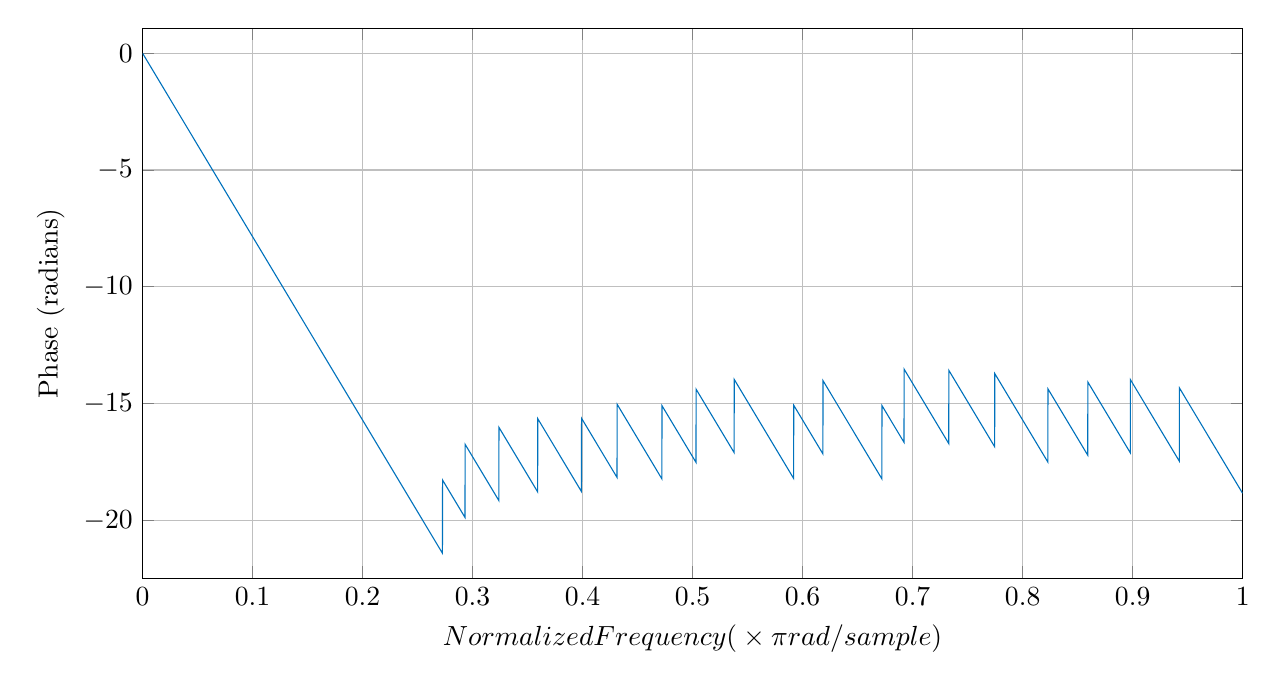
\begin{tikzpicture}

\begin{axis}[%
width=5.5in,
height=2.75in,
at={(1.281in,0.447in)},
scale only axis,
xmin=0,
xmax=0.9998779296875,
xlabel={$\text{Normalized Frequency (}\times\pi\text{ rad/sample)}$},
xmajorgrids,
ymin=-22.479050339472,
ymax=1.07043096854628,
ylabel={Phase (radians)},
ymajorgrids,
axis background/.style={fill=white},
]
\addplot [color=mycolor1,solid,forget plot]
  table[row sep=crcr]{%
0	0\\
0.0001220703125	-0.00958737992428528\\
0.000244140625	-0.0191747598485705\\
0.0003662109375	-0.0287621397728558\\
0.00048828125	-0.038349519697141\\
0.0006103515625	-0.0479368996214263\\
0.000732421875	-0.0575242795457115\\
0.0008544921875	-0.0671116594699968\\
0.0009765625	-0.076699039394282\\
0.0010986328125	-0.0862864193185673\\
0.001220703125	-0.0958737992428526\\
0.0013427734375	-0.105461179167138\\
0.00146484375	-0.115048559091423\\
0.0015869140625	-0.124635939015708\\
0.001708984375	-0.134223318939994\\
0.0018310546875	-0.143810698864279\\
0.001953125	-0.153398078788564\\
0.0020751953125	-0.162985458712849\\
0.002197265625	-0.172572838637135\\
0.0023193359375	-0.18216021856142\\
0.00244140625	-0.191747598485705\\
0.0025634765625	-0.20133497840999\\
0.002685546875	-0.210922358334276\\
0.0028076171875	-0.220509738258561\\
0.0029296875	-0.230097118182846\\
0.0030517578125	-0.239684498107131\\
0.003173828125	-0.249271878031417\\
0.0032958984375	-0.258859257955702\\
0.00341796875	-0.268446637879987\\
0.0035400390625	-0.278034017804273\\
0.003662109375	-0.287621397728558\\
0.0037841796875	-0.297208777652843\\
0.00390625	-0.306796157577128\\
0.0040283203125	-0.316383537501414\\
0.004150390625	-0.325970917425699\\
0.0042724609375	-0.335558297349984\\
0.00439453125	-0.345145677274269\\
0.0045166015625	-0.354733057198555\\
0.004638671875	-0.36432043712284\\
0.0047607421875	-0.373907817047125\\
0.0048828125	-0.38349519697141\\
0.0050048828125	-0.393082576895696\\
0.005126953125	-0.402669956819981\\
0.0052490234375	-0.412257336744266\\
0.00537109375	-0.421844716668551\\
0.0054931640625	-0.431432096592836\\
0.005615234375	-0.441019476517122\\
0.0057373046875	-0.450606856441407\\
0.005859375	-0.460194236365692\\
0.0059814453125	-0.469781616289978\\
0.006103515625	-0.479368996214263\\
0.0062255859375	-0.488956376138548\\
0.00634765625	-0.498543756062833\\
0.0064697265625	-0.508131135987119\\
0.006591796875	-0.517718515911404\\
0.0067138671875	-0.527305895835689\\
0.0068359375	-0.536893275759974\\
0.0069580078125	-0.54648065568426\\
0.007080078125	-0.556068035608545\\
0.0072021484375	-0.56565541553283\\
0.00732421875	-0.575242795457115\\
0.0074462890625	-0.584830175381401\\
0.007568359375	-0.594417555305686\\
0.0076904296875	-0.604004935229971\\
0.0078125	-0.613592315154257\\
0.0079345703125	-0.623179695078542\\
0.008056640625	-0.632767075002827\\
0.0081787109375	-0.642354454927112\\
0.00830078125	-0.651941834851398\\
0.0084228515625	-0.661529214775683\\
0.008544921875	-0.671116594699968\\
0.0086669921875	-0.680703974624253\\
0.0087890625	-0.690291354548539\\
0.0089111328125	-0.699878734472824\\
0.009033203125	-0.709466114397109\\
0.0091552734375	-0.719053494321394\\
0.00927734375	-0.72864087424568\\
0.0093994140625	-0.738228254169965\\
0.009521484375	-0.74781563409425\\
0.0096435546875	-0.757403014018535\\
0.009765625	-0.766990393942821\\
0.0098876953125	-0.776577773867106\\
0.010009765625	-0.786165153791391\\
0.0101318359375	-0.795752533715676\\
0.01025390625	-0.805339913639962\\
0.0103759765625	-0.814927293564247\\
0.010498046875	-0.824514673488532\\
0.0106201171875	-0.834102053412818\\
0.0107421875	-0.843689433337103\\
0.0108642578125	-0.853276813261388\\
0.010986328125	-0.862864193185673\\
0.0111083984375	-0.872451573109958\\
0.01123046875	-0.882038953034244\\
0.0113525390625	-0.891626332958529\\
0.011474609375	-0.901213712882814\\
0.0115966796875	-0.9108010928071\\
0.01171875	-0.920388472731385\\
0.0118408203125	-0.92997585265567\\
0.011962890625	-0.939563232579955\\
0.0120849609375	-0.94915061250424\\
0.01220703125	-0.958737992428526\\
0.0123291015625	-0.968325372352811\\
0.012451171875	-0.977912752277096\\
0.0125732421875	-0.987500132201382\\
0.0126953125	-0.997087512125667\\
0.0128173828125	-1.00667489204995\\
0.012939453125	-1.01626227197424\\
0.0130615234375	-1.02584965189852\\
0.01318359375	-1.03543703182281\\
0.0133056640625	-1.04502441174709\\
0.013427734375	-1.05461179167138\\
0.0135498046875	-1.06419917159566\\
0.013671875	-1.07378655151995\\
0.0137939453125	-1.08337393144423\\
0.013916015625	-1.09296131136852\\
0.0140380859375	-1.1025486912928\\
0.01416015625	-1.11213607121709\\
0.0142822265625	-1.12172345114137\\
0.014404296875	-1.13131083106566\\
0.0145263671875	-1.14089821098995\\
0.0146484375	-1.15048559091423\\
0.0147705078125	-1.16007297083852\\
0.014892578125	-1.1696603507628\\
0.0150146484375	-1.17924773068709\\
0.01513671875	-1.18883511061137\\
0.0152587890625	-1.19842249053566\\
0.015380859375	-1.20800987045994\\
0.0155029296875	-1.21759725038423\\
0.015625	-1.22718463030851\\
0.0157470703125	-1.2367720102328\\
0.015869140625	-1.24635939015708\\
0.0159912109375	-1.25594677008137\\
0.01611328125	-1.26553415000565\\
0.0162353515625	-1.27512152992994\\
0.016357421875	-1.28470890985422\\
0.0164794921875	-1.29429628977851\\
0.0166015625	-1.30388366970279\\
0.0167236328125	-1.31347104962708\\
0.016845703125	-1.32305842955137\\
0.0169677734375	-1.33264580947565\\
0.01708984375	-1.34223318939994\\
0.0172119140625	-1.35182056932422\\
0.017333984375	-1.36140794924851\\
0.0174560546875	-1.37099532917279\\
0.017578125	-1.38058270909708\\
0.0177001953125	-1.39017008902136\\
0.017822265625	-1.39975746894565\\
0.0179443359375	-1.40934484886993\\
0.01806640625	-1.41893222879422\\
0.0181884765625	-1.4285196087185\\
0.018310546875	-1.43810698864279\\
0.0184326171875	-1.44769436856707\\
0.0185546875	-1.45728174849136\\
0.0186767578125	-1.46686912841564\\
0.018798828125	-1.47645650833993\\
0.0189208984375	-1.48604388826421\\
0.01904296875	-1.4956312681885\\
0.0191650390625	-1.50521864811279\\
0.019287109375	-1.51480602803707\\
0.0194091796875	-1.52439340796136\\
0.01953125	-1.53398078788564\\
0.0196533203125	-1.54356816780993\\
0.019775390625	-1.55315554773421\\
0.0198974609375	-1.5627429276585\\
0.02001953125	-1.57233030758278\\
0.0201416015625	-1.58191768750707\\
0.020263671875	-1.59150506743135\\
0.0203857421875	-1.60109244735564\\
0.0205078125	-1.61067982727992\\
0.0206298828125	-1.62026720720421\\
0.020751953125	-1.62985458712849\\
0.0208740234375	-1.63944196705278\\
0.02099609375	-1.64902934697706\\
0.0211181640625	-1.65861672690135\\
0.021240234375	-1.66820410682564\\
0.0213623046875	-1.67779148674992\\
0.021484375	-1.68737886667421\\
0.0216064453125	-1.69696624659849\\
0.021728515625	-1.70655362652278\\
0.0218505859375	-1.71614100644706\\
0.02197265625	-1.72572838637135\\
0.0220947265625	-1.73531576629563\\
0.022216796875	-1.74490314621992\\
0.0223388671875	-1.7544905261442\\
0.0224609375	-1.76407790606849\\
0.0225830078125	-1.77366528599277\\
0.022705078125	-1.78325266591706\\
0.0228271484375	-1.79284004584134\\
0.02294921875	-1.80242742576563\\
0.0230712890625	-1.81201480568991\\
0.023193359375	-1.8216021856142\\
0.0233154296875	-1.83118956553848\\
0.0234375	-1.84077694546277\\
0.0235595703125	-1.85036432538705\\
0.023681640625	-1.85995170531134\\
0.0238037109375	-1.86953908523563\\
0.02392578125	-1.87912646515991\\
0.0240478515625	-1.8887138450842\\
0.024169921875	-1.89830122500848\\
0.0242919921875	-1.90788860493277\\
0.0244140625	-1.91747598485705\\
0.0245361328125	-1.92706336478134\\
0.024658203125	-1.93665074470562\\
0.0247802734375	-1.94623812462991\\
0.02490234375	-1.95582550455419\\
0.0250244140625	-1.96541288447848\\
0.025146484375	-1.97500026440276\\
0.0252685546875	-1.98458764432705\\
0.025390625	-1.99417502425133\\
0.0255126953125	-2.00376240417562\\
0.025634765625	-2.0133497840999\\
0.0257568359375	-2.02293716402419\\
0.02587890625	-2.03252454394847\\
0.0260009765625	-2.04211192387276\\
0.026123046875	-2.05169930379705\\
0.0262451171875	-2.06128668372133\\
0.0263671875	-2.07087406364562\\
0.0264892578125	-2.0804614435699\\
0.026611328125	-2.09004882349419\\
0.0267333984375	-2.09963620341847\\
0.02685546875	-2.10922358334276\\
0.0269775390625	-2.11881096326704\\
0.027099609375	-2.12839834319133\\
0.0272216796875	-2.13798572311561\\
0.02734375	-2.1475731030399\\
0.0274658203125	-2.15716048296418\\
0.027587890625	-2.16674786288847\\
0.0277099609375	-2.17633524281275\\
0.02783203125	-2.18592262273704\\
0.0279541015625	-2.19551000266132\\
0.028076171875	-2.20509738258561\\
0.0281982421875	-2.21468476250989\\
0.0283203125	-2.22427214243418\\
0.0284423828125	-2.23385952235847\\
0.028564453125	-2.24344690228275\\
0.0286865234375	-2.25303428220704\\
0.02880859375	-2.26262166213132\\
0.0289306640625	-2.27220904205561\\
0.029052734375	-2.28179642197989\\
0.0291748046875	-2.29138380190418\\
0.029296875	-2.30097118182846\\
0.0294189453125	-2.31055856175275\\
0.029541015625	-2.32014594167703\\
0.0296630859375	-2.32973332160132\\
0.02978515625	-2.3393207015256\\
0.0299072265625	-2.34890808144989\\
0.030029296875	-2.35849546137417\\
0.0301513671875	-2.36808284129846\\
0.0302734375	-2.37767022122274\\
0.0303955078125	-2.38725760114703\\
0.030517578125	-2.39684498107131\\
0.0306396484375	-2.4064323609956\\
0.03076171875	-2.41601974091988\\
0.0308837890625	-2.42560712084417\\
0.031005859375	-2.43519450076846\\
0.0311279296875	-2.44478188069274\\
0.03125	-2.45436926061703\\
0.0313720703125	-2.46395664054131\\
0.031494140625	-2.4735440204656\\
0.0316162109375	-2.48313140038988\\
0.03173828125	-2.49271878031417\\
0.0318603515625	-2.50230616023845\\
0.031982421875	-2.51189354016274\\
0.0321044921875	-2.52148092008702\\
0.0322265625	-2.53106830001131\\
0.0323486328125	-2.54065567993559\\
0.032470703125	-2.55024305985988\\
0.0325927734375	-2.55983043978416\\
0.03271484375	-2.56941781970845\\
0.0328369140625	-2.57900519963273\\
0.032958984375	-2.58859257955702\\
0.0330810546875	-2.59817995948131\\
0.033203125	-2.60776733940559\\
0.0333251953125	-2.61735471932988\\
0.033447265625	-2.62694209925416\\
0.0335693359375	-2.63652947917845\\
0.03369140625	-2.64611685910273\\
0.0338134765625	-2.65570423902702\\
0.033935546875	-2.6652916189513\\
0.0340576171875	-2.67487899887559\\
0.0341796875	-2.68446637879987\\
0.0343017578125	-2.69405375872416\\
0.034423828125	-2.70364113864844\\
0.0345458984375	-2.71322851857273\\
0.03466796875	-2.72281589849701\\
0.0347900390625	-2.7324032784213\\
0.034912109375	-2.74199065834558\\
0.0350341796875	-2.75157803826987\\
0.03515625	-2.76116541819415\\
0.0352783203125	-2.77075279811844\\
0.035400390625	-2.78034017804272\\
0.0355224609375	-2.78992755796701\\
0.03564453125	-2.7995149378913\\
0.0357666015625	-2.80910231781558\\
0.035888671875	-2.81868969773987\\
0.0360107421875	-2.82827707766415\\
0.0361328125	-2.83786445758844\\
0.0362548828125	-2.84745183751272\\
0.036376953125	-2.85703921743701\\
0.0364990234375	-2.86662659736129\\
0.03662109375	-2.87621397728558\\
0.0367431640625	-2.88580135720986\\
0.036865234375	-2.89538873713415\\
0.0369873046875	-2.90497611705843\\
0.037109375	-2.91456349698272\\
0.0372314453125	-2.924150876907\\
0.037353515625	-2.93373825683129\\
0.0374755859375	-2.94332563675557\\
0.03759765625	-2.95291301667986\\
0.0377197265625	-2.96250039660414\\
0.037841796875	-2.97208777652843\\
0.0379638671875	-2.98167515645272\\
0.0380859375	-2.991262536377\\
0.0382080078125	-3.00084991630129\\
0.038330078125	-3.01043729622557\\
0.0384521484375	-3.02002467614986\\
0.03857421875	-3.02961205607414\\
0.0386962890625	-3.03919943599843\\
0.038818359375	-3.04878681592271\\
0.0389404296875	-3.058374195847\\
0.0390625	-3.06796157577128\\
0.0391845703125	-3.07754895569557\\
0.039306640625	-3.08713633561985\\
0.0394287109375	-3.09672371554414\\
0.03955078125	-3.10631109546842\\
0.0396728515625	-3.11589847539271\\
0.039794921875	-3.12548585531699\\
0.0399169921875	-3.13507323524128\\
0.0400390625	-3.14466061516556\\
0.0401611328125	-3.15424799508985\\
0.040283203125	-3.16383537501413\\
0.0404052734375	-3.17342275493842\\
0.04052734375	-3.18301013486271\\
0.0406494140625	-3.19259751478699\\
0.040771484375	-3.20218489471128\\
0.0408935546875	-3.21177227463556\\
0.041015625	-3.22135965455985\\
0.0411376953125	-3.23094703448413\\
0.041259765625	-3.24053441440842\\
0.0413818359375	-3.2501217943327\\
0.04150390625	-3.25970917425699\\
0.0416259765625	-3.26929655418127\\
0.041748046875	-3.27888393410556\\
0.0418701171875	-3.28847131402984\\
0.0419921875	-3.29805869395413\\
0.0421142578125	-3.30764607387841\\
0.042236328125	-3.3172334538027\\
0.0423583984375	-3.32682083372698\\
0.04248046875	-3.33640821365127\\
0.0426025390625	-3.34599559357555\\
0.042724609375	-3.35558297349984\\
0.0428466796875	-3.36517035342413\\
0.04296875	-3.37475773334841\\
0.0430908203125	-3.3843451132727\\
0.043212890625	-3.39393249319698\\
0.0433349609375	-3.40351987312127\\
0.04345703125	-3.41310725304555\\
0.0435791015625	-3.42269463296984\\
0.043701171875	-3.43228201289412\\
0.0438232421875	-3.44186939281841\\
0.0439453125	-3.45145677274269\\
0.0440673828125	-3.46104415266698\\
0.044189453125	-3.47063153259126\\
0.0443115234375	-3.48021891251555\\
0.04443359375	-3.48980629243983\\
0.0445556640625	-3.49939367236412\\
0.044677734375	-3.5089810522884\\
0.0447998046875	-3.51856843221269\\
0.044921875	-3.52815581213697\\
0.0450439453125	-3.53774319206126\\
0.045166015625	-3.54733057198555\\
0.0452880859375	-3.55691795190983\\
0.04541015625	-3.56650533183412\\
0.0455322265625	-3.5760927117584\\
0.045654296875	-3.58568009168269\\
0.0457763671875	-3.59526747160697\\
0.0458984375	-3.60485485153126\\
0.0460205078125	-3.61444223145554\\
0.046142578125	-3.62402961137983\\
0.0462646484375	-3.63361699130411\\
0.04638671875	-3.6432043712284\\
0.0465087890625	-3.65279175115268\\
0.046630859375	-3.66237913107697\\
0.0467529296875	-3.67196651100125\\
0.046875	-3.68155389092554\\
0.0469970703125	-3.69114127084982\\
0.047119140625	-3.70072865077411\\
0.0472412109375	-3.71031603069839\\
0.04736328125	-3.71990341062268\\
0.0474853515625	-3.72949079054697\\
0.047607421875	-3.73907817047125\\
0.0477294921875	-3.74866555039554\\
0.0478515625	-3.75825293031982\\
0.0479736328125	-3.76784031024411\\
0.048095703125	-3.77742769016839\\
0.0482177734375	-3.78701507009268\\
0.04833984375	-3.79660245001696\\
0.0484619140625	-3.80618982994125\\
0.048583984375	-3.81577720986553\\
0.0487060546875	-3.82536458978982\\
0.048828125	-3.8349519697141\\
0.0489501953125	-3.84453934963839\\
0.049072265625	-3.85412672956267\\
0.0491943359375	-3.86371410948696\\
0.04931640625	-3.87330148941124\\
0.0494384765625	-3.88288886933553\\
0.049560546875	-3.89247624925981\\
0.0496826171875	-3.9020636291841\\
0.0498046875	-3.91165100910839\\
0.0499267578125	-3.92123838903267\\
0.050048828125	-3.93082576895696\\
0.0501708984375	-3.94041314888124\\
0.05029296875	-3.95000052880553\\
0.0504150390625	-3.95958790872981\\
0.050537109375	-3.9691752886541\\
0.0506591796875	-3.97876266857838\\
0.05078125	-3.98835004850267\\
0.0509033203125	-3.99793742842695\\
0.051025390625	-4.00752480835124\\
0.0511474609375	-4.01711218827552\\
0.05126953125	-4.02669956819981\\
0.0513916015625	-4.03628694812409\\
0.051513671875	-4.04587432804838\\
0.0516357421875	-4.05546170797266\\
0.0517578125	-4.06504908789695\\
0.0518798828125	-4.07463646782123\\
0.052001953125	-4.08422384774552\\
0.0521240234375	-4.09381122766981\\
0.05224609375	-4.10339860759409\\
0.0523681640625	-4.11298598751837\\
0.052490234375	-4.12257336744266\\
0.0526123046875	-4.13216074736695\\
0.052734375	-4.14174812729123\\
0.0528564453125	-4.15133550721552\\
0.052978515625	-4.1609228871398\\
0.0531005859375	-4.17051026706409\\
0.05322265625	-4.18009764698837\\
0.0533447265625	-4.18968502691266\\
0.053466796875	-4.19927240683694\\
0.0535888671875	-4.20885978676123\\
0.0537109375	-4.21844716668551\\
0.0538330078125	-4.2280345466098\\
0.053955078125	-4.23762192653408\\
0.0540771484375	-4.24720930645837\\
0.05419921875	-4.25679668638265\\
0.0543212890625	-4.26638406630694\\
0.054443359375	-4.27597144623122\\
0.0545654296875	-4.28555882615551\\
0.0546875	-4.29514620607979\\
0.0548095703125	-4.30473358600408\\
0.054931640625	-4.31432096592837\\
0.0550537109375	-4.32390834585265\\
0.05517578125	-4.33349572577694\\
0.0552978515625	-4.34308310570122\\
0.055419921875	-4.35267048562551\\
0.0555419921875	-4.36225786554979\\
0.0556640625	-4.37184524547408\\
0.0557861328125	-4.38143262539836\\
0.055908203125	-4.39102000532265\\
0.0560302734375	-4.40060738524693\\
0.05615234375	-4.41019476517122\\
0.0562744140625	-4.4197821450955\\
0.056396484375	-4.42936952501979\\
0.0565185546875	-4.43895690494407\\
0.056640625	-4.44854428486836\\
0.0567626953125	-4.45813166479264\\
0.056884765625	-4.46771904471693\\
0.0570068359375	-4.47730642464122\\
0.05712890625	-4.4868938045655\\
0.0572509765625	-4.49648118448979\\
0.057373046875	-4.50606856441407\\
0.0574951171875	-4.51565594433836\\
0.0576171875	-4.52524332426264\\
0.0577392578125	-4.53483070418693\\
0.057861328125	-4.54441808411121\\
0.0579833984375	-4.5540054640355\\
0.05810546875	-4.56359284395978\\
0.0582275390625	-4.57318022388407\\
0.058349609375	-4.58276760380835\\
0.0584716796875	-4.59235498373264\\
0.05859375	-4.60194236365692\\
0.0587158203125	-4.61152974358121\\
0.058837890625	-4.62111712350549\\
0.0589599609375	-4.63070450342978\\
0.05908203125	-4.64029188335406\\
0.0592041015625	-4.64987926327835\\
0.059326171875	-4.65946664320263\\
0.0594482421875	-4.66905402312692\\
0.0595703125	-4.67864140305121\\
0.0596923828125	-4.68822878297549\\
0.059814453125	-4.69781616289978\\
0.0599365234375	-4.70740354282406\\
0.06005859375	-4.71699092274835\\
0.0601806640625	-4.72657830267263\\
0.060302734375	-4.73616568259692\\
0.0604248046875	-4.7457530625212\\
0.060546875	-4.75534044244549\\
0.0606689453125	-4.76492782236977\\
0.060791015625	-4.77451520229406\\
0.0609130859375	-4.78410258221834\\
0.06103515625	-4.79368996214263\\
0.0611572265625	-4.80327734206691\\
0.061279296875	-4.8128647219912\\
0.0614013671875	-4.82245210191548\\
0.0615234375	-4.83203948183977\\
0.0616455078125	-4.84162686176405\\
0.061767578125	-4.85121424168834\\
0.0618896484375	-4.86080162161262\\
0.06201171875	-4.87038900153691\\
0.0621337890625	-4.8799763814612\\
0.062255859375	-4.88956376138548\\
0.0623779296875	-4.89915114130977\\
0.0625	-4.90873852123405\\
0.0626220703125	-4.91832590115834\\
0.062744140625	-4.92791328108262\\
0.0628662109375	-4.93750066100691\\
0.06298828125	-4.94708804093119\\
0.0631103515625	-4.95667542085548\\
0.063232421875	-4.96626280077976\\
0.0633544921875	-4.97585018070405\\
0.0634765625	-4.98543756062833\\
0.0635986328125	-4.99502494055262\\
0.063720703125	-5.0046123204769\\
0.0638427734375	-5.01419970040119\\
0.06396484375	-5.02378708032547\\
0.0640869140625	-5.03337446024976\\
0.064208984375	-5.04296184017405\\
0.0643310546875	-5.05254922009833\\
0.064453125	-5.06213660002262\\
0.0645751953125	-5.0717239799469\\
0.064697265625	-5.08131135987119\\
0.0648193359375	-5.09089873979547\\
0.06494140625	-5.10048611971976\\
0.0650634765625	-5.11007349964404\\
0.065185546875	-5.11966087956833\\
0.0653076171875	-5.12924825949261\\
0.0654296875	-5.1388356394169\\
0.0655517578125	-5.14842301934118\\
0.065673828125	-5.15801039926547\\
0.0657958984375	-5.16759777918975\\
0.06591796875	-5.17718515911404\\
0.0660400390625	-5.18677253903832\\
0.066162109375	-5.19635991896261\\
0.0662841796875	-5.20594729888689\\
0.06640625	-5.21553467881118\\
0.0665283203125	-5.22512205873547\\
0.066650390625	-5.23470943865975\\
0.0667724609375	-5.24429681858404\\
0.06689453125	-5.25388419850832\\
0.0670166015625	-5.26347157843261\\
0.067138671875	-5.27305895835689\\
0.0672607421875	-5.28264633828118\\
0.0673828125	-5.29223371820546\\
0.0675048828125	-5.30182109812975\\
0.067626953125	-5.31140847805403\\
0.0677490234375	-5.32099585797832\\
0.06787109375	-5.3305832379026\\
0.0679931640625	-5.34017061782689\\
0.068115234375	-5.34975799775117\\
0.0682373046875	-5.35934537767546\\
0.068359375	-5.36893275759974\\
0.0684814453125	-5.37852013752403\\
0.068603515625	-5.38810751744832\\
0.0687255859375	-5.3976948973726\\
0.06884765625	-5.40728227729689\\
0.0689697265625	-5.41686965722117\\
0.069091796875	-5.42645703714546\\
0.0692138671875	-5.43604441706974\\
0.0693359375	-5.44563179699403\\
0.0694580078125	-5.45521917691831\\
0.069580078125	-5.4648065568426\\
0.0697021484375	-5.47439393676688\\
0.06982421875	-5.48398131669117\\
0.0699462890625	-5.49356869661545\\
0.070068359375	-5.50315607653974\\
0.0701904296875	-5.51274345646402\\
0.0703125	-5.52233083638831\\
0.0704345703125	-5.53191821631259\\
0.070556640625	-5.54150559623688\\
0.0706787109375	-5.55109297616116\\
0.07080078125	-5.56068035608545\\
0.0709228515625	-5.57026773600973\\
0.071044921875	-5.57985511593402\\
0.0711669921875	-5.5894424958583\\
0.0712890625	-5.59902987578259\\
0.0714111328125	-5.60861725570688\\
0.071533203125	-5.61820463563116\\
0.0716552734375	-5.62779201555545\\
0.07177734375	-5.63737939547973\\
0.0718994140625	-5.64696677540402\\
0.072021484375	-5.6565541553283\\
0.0721435546875	-5.66614153525259\\
0.072265625	-5.67572891517687\\
0.0723876953125	-5.68531629510116\\
0.072509765625	-5.69490367502544\\
0.0726318359375	-5.70449105494973\\
0.07275390625	-5.71407843487401\\
0.0728759765625	-5.7236658147983\\
0.072998046875	-5.73325319472258\\
0.0731201171875	-5.74284057464687\\
0.0732421875	-5.75242795457115\\
0.0733642578125	-5.76201533449544\\
0.073486328125	-5.77160271441972\\
0.0736083984375	-5.78119009434401\\
0.07373046875	-5.7907774742683\\
0.0738525390625	-5.80036485419258\\
0.073974609375	-5.80995223411687\\
0.0740966796875	-5.81953961404115\\
0.07421875	-5.82912699396544\\
0.0743408203125	-5.83871437388972\\
0.074462890625	-5.84830175381401\\
0.0745849609375	-5.85788913373829\\
0.07470703125	-5.86747651366258\\
0.0748291015625	-5.87706389358686\\
0.074951171875	-5.88665127351115\\
0.0750732421875	-5.89623865343543\\
0.0751953125	-5.90582603335972\\
0.0753173828125	-5.915413413284\\
0.075439453125	-5.92500079320829\\
0.0755615234375	-5.93458817313257\\
0.07568359375	-5.94417555305686\\
0.0758056640625	-5.95376293298115\\
0.075927734375	-5.96335031290543\\
0.0760498046875	-5.97293769282972\\
0.076171875	-5.982525072754\\
0.0762939453125	-5.99211245267829\\
0.076416015625	-6.00169983260257\\
0.0765380859375	-6.01128721252686\\
0.07666015625	-6.02087459245114\\
0.0767822265625	-6.03046197237543\\
0.076904296875	-6.04004935229971\\
0.0770263671875	-6.049636732224\\
0.0771484375	-6.05922411214828\\
0.0772705078125	-6.06881149207257\\
0.077392578125	-6.07839887199685\\
0.0775146484375	-6.08798625192114\\
0.07763671875	-6.09757363184542\\
0.0777587890625	-6.10716101176971\\
0.077880859375	-6.11674839169399\\
0.0780029296875	-6.12633577161828\\
0.078125	-6.13592315154256\\
0.0782470703125	-6.14551053146685\\
0.078369140625	-6.15509791139114\\
0.0784912109375	-6.16468529131542\\
0.07861328125	-6.17427267123971\\
0.0787353515625	-6.18386005116399\\
0.078857421875	-6.19344743108828\\
0.0789794921875	-6.20303481101256\\
0.0791015625	-6.21262219093685\\
0.0792236328125	-6.22220957086113\\
0.079345703125	-6.23179695078542\\
0.0794677734375	-6.2413843307097\\
0.07958984375	-6.25097171063399\\
0.0797119140625	-6.26055909055827\\
0.079833984375	-6.27014647048256\\
0.0799560546875	-6.27973385040684\\
0.080078125	-6.28932123033113\\
0.0802001953125	-6.29890861025541\\
0.080322265625	-6.3084959901797\\
0.0804443359375	-6.31808337010398\\
0.08056640625	-6.32767075002827\\
0.0806884765625	-6.33725812995255\\
0.080810546875	-6.34684550987684\\
0.0809326171875	-6.35643288980113\\
0.0810546875	-6.36602026972541\\
0.0811767578125	-6.3756076496497\\
0.081298828125	-6.38519502957398\\
0.0814208984375	-6.39478240949827\\
0.08154296875	-6.40436978942255\\
0.0816650390625	-6.41395716934684\\
0.081787109375	-6.42354454927112\\
0.0819091796875	-6.43313192919541\\
0.08203125	-6.44271930911969\\
0.0821533203125	-6.45230668904398\\
0.082275390625	-6.46189406896826\\
0.0823974609375	-6.47148144889255\\
0.08251953125	-6.48106882881683\\
0.0826416015625	-6.49065620874112\\
0.082763671875	-6.5002435886654\\
0.0828857421875	-6.50983096858969\\
0.0830078125	-6.51941834851397\\
0.0831298828125	-6.52900572843826\\
0.083251953125	-6.53859310836255\\
0.0833740234375	-6.54818048828683\\
0.08349609375	-6.55776786821112\\
0.0836181640625	-6.5673552481354\\
0.083740234375	-6.57694262805969\\
0.0838623046875	-6.58653000798397\\
0.083984375	-6.59611738790826\\
0.0841064453125	-6.60570476783254\\
0.084228515625	-6.61529214775683\\
0.0843505859375	-6.62487952768111\\
0.08447265625	-6.6344669076054\\
0.0845947265625	-6.64405428752968\\
0.084716796875	-6.65364166745397\\
0.0848388671875	-6.66322904737825\\
0.0849609375	-6.67281642730254\\
0.0850830078125	-6.68240380722682\\
0.085205078125	-6.69199118715111\\
0.0853271484375	-6.7015785670754\\
0.08544921875	-6.71116594699968\\
0.0855712890625	-6.72075332692397\\
0.085693359375	-6.73034070684825\\
0.0858154296875	-6.73992808677254\\
0.0859375	-6.74951546669682\\
0.0860595703125	-6.75910284662111\\
0.086181640625	-6.76869022654539\\
0.0863037109375	-6.77827760646968\\
0.08642578125	-6.78786498639396\\
0.0865478515625	-6.79745236631825\\
0.086669921875	-6.80703974624253\\
0.0867919921875	-6.81662712616682\\
0.0869140625	-6.8262145060911\\
0.0870361328125	-6.83580188601539\\
0.087158203125	-6.84538926593967\\
0.0872802734375	-6.85497664586396\\
0.08740234375	-6.86456402578824\\
0.0875244140625	-6.87415140571253\\
0.087646484375	-6.88373878563681\\
0.0877685546875	-6.8933261655611\\
0.087890625	-6.90291354548539\\
0.0880126953125	-6.91250092540967\\
0.088134765625	-6.92208830533396\\
0.0882568359375	-6.93167568525824\\
0.08837890625	-6.94126306518253\\
0.0885009765625	-6.95085044510681\\
0.088623046875	-6.9604378250311\\
0.0887451171875	-6.97002520495538\\
0.0888671875	-6.97961258487967\\
0.0889892578125	-6.98919996480395\\
0.089111328125	-6.99878734472824\\
0.0892333984375	-7.00837472465252\\
0.08935546875	-7.01796210457681\\
0.0894775390625	-7.02754948450109\\
0.089599609375	-7.03713686442538\\
0.0897216796875	-7.04672424434966\\
0.08984375	-7.05631162427395\\
0.0899658203125	-7.06589900419823\\
0.090087890625	-7.07548638412252\\
0.0902099609375	-7.0850737640468\\
0.09033203125	-7.09466114397109\\
0.0904541015625	-7.10424852389538\\
0.090576171875	-7.11383590381966\\
0.0906982421875	-7.12342328374395\\
0.0908203125	-7.13301066366823\\
0.0909423828125	-7.14259804359252\\
0.091064453125	-7.1521854235168\\
0.0911865234375	-7.16177280344109\\
0.09130859375	-7.17136018336537\\
0.0914306640625	-7.18094756328966\\
0.091552734375	-7.19053494321394\\
0.0916748046875	-7.20012232313823\\
0.091796875	-7.20970970306251\\
0.0919189453125	-7.2192970829868\\
0.092041015625	-7.22888446291108\\
0.0921630859375	-7.23847184283537\\
0.09228515625	-7.24805922275965\\
0.0924072265625	-7.25764660268394\\
0.092529296875	-7.26723398260823\\
0.0926513671875	-7.27682136253251\\
0.0927734375	-7.2864087424568\\
0.0928955078125	-7.29599612238108\\
0.093017578125	-7.30558350230537\\
0.0931396484375	-7.31517088222965\\
0.09326171875	-7.32475826215394\\
0.0933837890625	-7.33434564207822\\
0.093505859375	-7.34393302200251\\
0.0936279296875	-7.35352040192679\\
0.09375	-7.36310778185108\\
0.0938720703125	-7.37269516177536\\
0.093994140625	-7.38228254169965\\
0.0941162109375	-7.39186992162393\\
0.09423828125	-7.40145730154822\\
0.0943603515625	-7.4110446814725\\
0.094482421875	-7.42063206139679\\
0.0946044921875	-7.43021944132107\\
0.0947265625	-7.43980682124536\\
0.0948486328125	-7.44939420116965\\
0.094970703125	-7.45898158109393\\
0.0950927734375	-7.46856896101822\\
0.09521484375	-7.4781563409425\\
0.0953369140625	-7.48774372086679\\
0.095458984375	-7.49733110079107\\
0.0955810546875	-7.50691848071536\\
0.095703125	-7.51650586063964\\
0.0958251953125	-7.52609324056393\\
0.095947265625	-7.53568062048821\\
0.0960693359375	-7.5452680004125\\
0.09619140625	-7.55485538033678\\
0.0963134765625	-7.56444276026107\\
0.096435546875	-7.57403014018535\\
0.0965576171875	-7.58361752010964\\
0.0966796875	-7.59320490003392\\
0.0968017578125	-7.60279227995821\\
0.096923828125	-7.61237965988249\\
0.0970458984375	-7.62196703980678\\
0.09716796875	-7.63155441973106\\
0.0972900390625	-7.64114179965535\\
0.097412109375	-7.65072917957963\\
0.0975341796875	-7.66031655950392\\
0.09765625	-7.66990393942821\\
0.0977783203125	-7.67949131935249\\
0.097900390625	-7.68907869927678\\
0.0980224609375	-7.69866607920106\\
0.09814453125	-7.70825345912535\\
0.0982666015625	-7.71784083904963\\
0.098388671875	-7.72742821897392\\
0.0985107421875	-7.7370155988982\\
0.0986328125	-7.74660297882249\\
0.0987548828125	-7.75619035874677\\
0.098876953125	-7.76577773867106\\
0.0989990234375	-7.77536511859534\\
0.09912109375	-7.78495249851963\\
0.0992431640625	-7.79453987844391\\
0.099365234375	-7.8041272583682\\
0.0994873046875	-7.81371463829248\\
0.099609375	-7.82330201821677\\
0.0997314453125	-7.83288939814106\\
0.099853515625	-7.84247677806534\\
0.0999755859375	-7.85206415798963\\
0.10009765625	-7.86165153791391\\
0.1002197265625	-7.8712389178382\\
0.100341796875	-7.88082629776248\\
0.1004638671875	-7.89041367768677\\
0.1005859375	-7.90000105761105\\
0.1007080078125	-7.90958843753534\\
0.100830078125	-7.91917581745962\\
0.1009521484375	-7.92876319738391\\
0.10107421875	-7.93835057730819\\
0.1011962890625	-7.94793795723248\\
0.101318359375	-7.95752533715676\\
0.1014404296875	-7.96711271708105\\
0.1015625	-7.97670009700533\\
0.1016845703125	-7.98628747692962\\
0.101806640625	-7.9958748568539\\
0.1019287109375	-8.00546223677819\\
0.10205078125	-8.01504961670248\\
0.1021728515625	-8.02463699662676\\
0.102294921875	-8.03422437655105\\
0.1024169921875	-8.04381175647533\\
0.1025390625	-8.05339913639962\\
0.1026611328125	-8.0629865163239\\
0.102783203125	-8.07257389624819\\
0.1029052734375	-8.08216127617247\\
0.10302734375	-8.09174865609676\\
0.1031494140625	-8.10133603602104\\
0.103271484375	-8.11092341594533\\
0.1033935546875	-8.12051079586961\\
0.103515625	-8.1300981757939\\
0.1036376953125	-8.13968555571818\\
0.103759765625	-8.14927293564247\\
0.1038818359375	-8.15886031556675\\
0.10400390625	-8.16844769549104\\
0.1041259765625	-8.17803507541533\\
0.104248046875	-8.18762245533961\\
0.1043701171875	-8.19720983526389\\
0.1044921875	-8.20679721518818\\
0.1046142578125	-8.21638459511247\\
0.104736328125	-8.22597197503675\\
0.1048583984375	-8.23555935496104\\
0.10498046875	-8.24514673488532\\
0.1051025390625	-8.25473411480961\\
0.105224609375	-8.26432149473389\\
0.1053466796875	-8.27390887465818\\
0.10546875	-8.28349625458246\\
0.1055908203125	-8.29308363450675\\
0.105712890625	-8.30267101443103\\
0.1058349609375	-8.31225839435532\\
0.10595703125	-8.3218457742796\\
0.1060791015625	-8.33143315420389\\
0.106201171875	-8.34102053412817\\
0.1063232421875	-8.35060791405246\\
0.1064453125	-8.36019529397674\\
0.1065673828125	-8.36978267390103\\
0.106689453125	-8.37937005382532\\
0.1068115234375	-8.3889574337496\\
0.10693359375	-8.39854481367388\\
0.1070556640625	-8.40813219359817\\
0.107177734375	-8.41771957352246\\
0.1072998046875	-8.42730695344674\\
0.107421875	-8.43689433337103\\
0.1075439453125	-8.44648171329531\\
0.107666015625	-8.4560690932196\\
0.1077880859375	-8.46565647314388\\
0.10791015625	-8.47524385306817\\
0.1080322265625	-8.48483123299245\\
0.108154296875	-8.49441861291674\\
0.1082763671875	-8.50400599284102\\
0.1083984375	-8.51359337276531\\
0.1085205078125	-8.52318075268959\\
0.108642578125	-8.53276813261388\\
0.1087646484375	-8.54235551253817\\
0.10888671875	-8.55194289246245\\
0.1090087890625	-8.56153027238673\\
0.109130859375	-8.57111765231102\\
0.1092529296875	-8.5807050322353\\
0.109375	-8.59029241215959\\
0.1094970703125	-8.59987979208388\\
0.109619140625	-8.60946717200816\\
0.1097412109375	-8.61905455193245\\
0.10986328125	-8.62864193185673\\
0.1099853515625	-8.63822931178102\\
0.110107421875	-8.6478166917053\\
0.1102294921875	-8.65740407162959\\
0.1103515625	-8.66699145155387\\
0.1104736328125	-8.67657883147816\\
0.110595703125	-8.68616621140244\\
0.1107177734375	-8.69575359132673\\
0.11083984375	-8.70534097125101\\
0.1109619140625	-8.7149283511753\\
0.111083984375	-8.72451573109958\\
0.1112060546875	-8.73410311102387\\
0.111328125	-8.74369049094815\\
0.1114501953125	-8.75327787087244\\
0.111572265625	-8.76286525079673\\
0.1116943359375	-8.77245263072101\\
0.11181640625	-8.7820400106453\\
0.1119384765625	-8.79162739056958\\
0.112060546875	-8.80121477049387\\
0.1121826171875	-8.81080215041815\\
0.1123046875	-8.82038953034244\\
0.1124267578125	-8.82997691026672\\
0.112548828125	-8.83956429019101\\
0.1126708984375	-8.84915167011529\\
0.11279296875	-8.85873905003958\\
0.1129150390625	-8.86832642996386\\
0.113037109375	-8.87791380988815\\
0.1131591796875	-8.88750118981243\\
0.11328125	-8.89708856973672\\
0.1134033203125	-8.906675949661\\
0.113525390625	-8.91626332958529\\
0.1136474609375	-8.92585070950958\\
0.11376953125	-8.93543808943386\\
0.1138916015625	-8.94502546935815\\
0.114013671875	-8.95461284928243\\
0.1141357421875	-8.96420022920672\\
0.1142578125	-8.973787609131\\
0.1143798828125	-8.98337498905529\\
0.114501953125	-8.99296236897957\\
0.1146240234375	-9.00254974890386\\
0.11474609375	-9.01213712882814\\
0.1148681640625	-9.02172450875243\\
0.114990234375	-9.03131188867671\\
0.1151123046875	-9.040899268601\\
0.115234375	-9.05048664852528\\
0.1153564453125	-9.06007402844957\\
0.115478515625	-9.06966140837385\\
0.1156005859375	-9.07924878829814\\
0.11572265625	-9.08883616822243\\
0.1158447265625	-9.09842354814671\\
0.115966796875	-9.10801092807099\\
0.1160888671875	-9.11759830799528\\
0.1162109375	-9.12718568791957\\
0.1163330078125	-9.13677306784385\\
0.116455078125	-9.14636044776814\\
0.1165771484375	-9.15594782769242\\
0.11669921875	-9.16553520761671\\
0.1168212890625	-9.17512258754099\\
0.116943359375	-9.18470996746528\\
0.1170654296875	-9.19429734738956\\
0.1171875	-9.20388472731385\\
0.1173095703125	-9.21347210723813\\
0.117431640625	-9.22305948716242\\
0.1175537109375	-9.2326468670867\\
0.11767578125	-9.24223424701099\\
0.1177978515625	-9.25182162693527\\
0.117919921875	-9.26140900685956\\
0.1180419921875	-9.27099638678384\\
0.1181640625	-9.28058376670813\\
0.1182861328125	-9.29017114663241\\
0.118408203125	-9.2997585265567\\
0.1185302734375	-9.30934590648098\\
0.11865234375	-9.31893328640527\\
0.1187744140625	-9.32852066632956\\
0.118896484375	-9.33810804625384\\
0.1190185546875	-9.34769542617813\\
0.119140625	-9.35728280610241\\
0.1192626953125	-9.3668701860267\\
0.119384765625	-9.37645756595098\\
0.1195068359375	-9.38604494587527\\
0.11962890625	-9.39563232579955\\
0.1197509765625	-9.40521970572384\\
0.119873046875	-9.41480708564812\\
0.1199951171875	-9.42439446557241\\
0.1201171875	-9.43398184549669\\
0.1202392578125	-9.44356922542098\\
0.120361328125	-9.45315660534526\\
0.1204833984375	-9.46274398526955\\
0.12060546875	-9.47233136519383\\
0.1207275390625	-9.48191874511812\\
0.120849609375	-9.4915061250424\\
0.1209716796875	-9.50109350496669\\
0.12109375	-9.51068088489098\\
0.1212158203125	-9.52026826481526\\
0.121337890625	-9.52985564473954\\
0.1214599609375	-9.53944302466383\\
0.12158203125	-9.54903040458812\\
0.1217041015625	-9.5586177845124\\
0.121826171875	-9.56820516443669\\
0.1219482421875	-9.57779254436097\\
0.1220703125	-9.58737992428526\\
0.1221923828125	-9.59696730420954\\
0.122314453125	-9.60655468413383\\
0.1224365234375	-9.61614206405811\\
0.12255859375	-9.6257294439824\\
0.1226806640625	-9.63531682390668\\
0.122802734375	-9.64490420383097\\
0.1229248046875	-9.65449158375525\\
0.123046875	-9.66407896367954\\
0.1231689453125	-9.67366634360382\\
0.123291015625	-9.68325372352811\\
0.1234130859375	-9.69284110345239\\
0.12353515625	-9.70242848337668\\
0.1236572265625	-9.71201586330097\\
0.123779296875	-9.72160324322525\\
0.1239013671875	-9.73119062314954\\
0.1240234375	-9.74077800307382\\
0.1241455078125	-9.75036538299811\\
0.124267578125	-9.75995276292239\\
0.1243896484375	-9.76954014284668\\
0.12451171875	-9.77912752277096\\
0.1246337890625	-9.78871490269525\\
0.124755859375	-9.79830228261953\\
0.1248779296875	-9.80788966254382\\
0.125	-9.8174770424681\\
0.1251220703125	-9.82706442239239\\
0.125244140625	-9.83665180231667\\
0.1253662109375	-9.84623918224096\\
0.12548828125	-9.85582656216524\\
0.1256103515625	-9.86541394208953\\
0.125732421875	-9.87500132201382\\
0.1258544921875	-9.8845887019381\\
0.1259765625	-9.89417608186239\\
0.1260986328125	-9.90376346178667\\
0.126220703125	-9.91335084171096\\
0.1263427734375	-9.92293822163524\\
0.12646484375	-9.93252560155953\\
0.1265869140625	-9.94211298148381\\
0.126708984375	-9.9517003614081\\
0.1268310546875	-9.96128774133238\\
0.126953125	-9.97087512125667\\
0.1270751953125	-9.98046250118095\\
0.127197265625	-9.99004988110524\\
0.1273193359375	-9.99963726102952\\
0.12744140625	-10.0092246409538\\
0.1275634765625	-10.0188120208781\\
0.127685546875	-10.0283994008024\\
0.1278076171875	-10.0379867807267\\
0.1279296875	-10.0475741606509\\
0.1280517578125	-10.0571615405752\\
0.128173828125	-10.0667489204995\\
0.1282958984375	-10.0763363004238\\
0.12841796875	-10.0859236803481\\
0.1285400390625	-10.0955110602724\\
0.128662109375	-10.1050984401967\\
0.1287841796875	-10.1146858201209\\
0.12890625	-10.1242732000452\\
0.1290283203125	-10.1338605799695\\
0.129150390625	-10.1434479598938\\
0.1292724609375	-10.1530353398181\\
0.12939453125	-10.1626227197424\\
0.1295166015625	-10.1722100996667\\
0.129638671875	-10.1817974795909\\
0.1297607421875	-10.1913848595152\\
0.1298828125	-10.2009722394395\\
0.1300048828125	-10.2105596193638\\
0.130126953125	-10.2201469992881\\
0.1302490234375	-10.2297343792124\\
0.13037109375	-10.2393217591367\\
0.1304931640625	-10.2489091390609\\
0.130615234375	-10.2584965189852\\
0.1307373046875	-10.2680838989095\\
0.130859375	-10.2776712788338\\
0.1309814453125	-10.2872586587581\\
0.131103515625	-10.2968460386824\\
0.1312255859375	-10.3064334186067\\
0.13134765625	-10.3160207985309\\
0.1314697265625	-10.3256081784552\\
0.131591796875	-10.3351955583795\\
0.1317138671875	-10.3447829383038\\
0.1318359375	-10.3543703182281\\
0.1319580078125	-10.3639576981524\\
0.132080078125	-10.3735450780766\\
0.1322021484375	-10.3831324580009\\
0.13232421875	-10.3927198379252\\
0.1324462890625	-10.4023072178495\\
0.132568359375	-10.4118945977738\\
0.1326904296875	-10.4214819776981\\
0.1328125	-10.4310693576224\\
0.1329345703125	-10.4406567375466\\
0.133056640625	-10.4502441174709\\
0.1331787109375	-10.4598314973952\\
0.13330078125	-10.4694188773195\\
0.1334228515625	-10.4790062572438\\
0.133544921875	-10.4885936371681\\
0.1336669921875	-10.4981810170924\\
0.1337890625	-10.5077683970166\\
0.1339111328125	-10.5173557769409\\
0.134033203125	-10.5269431568652\\
0.1341552734375	-10.5365305367895\\
0.13427734375	-10.5461179167138\\
0.1343994140625	-10.5557052966381\\
0.134521484375	-10.5652926765624\\
0.1346435546875	-10.5748800564866\\
0.134765625	-10.5844674364109\\
0.1348876953125	-10.5940548163352\\
0.135009765625	-10.6036421962595\\
0.1351318359375	-10.6132295761838\\
0.13525390625	-10.6228169561081\\
0.1353759765625	-10.6324043360324\\
0.135498046875	-10.6419917159566\\
0.1356201171875	-10.6515790958809\\
0.1357421875	-10.6611664758052\\
0.1358642578125	-10.6707538557295\\
0.135986328125	-10.6803412356538\\
0.1361083984375	-10.6899286155781\\
0.13623046875	-10.6995159955023\\
0.1363525390625	-10.7091033754266\\
0.136474609375	-10.7186907553509\\
0.1365966796875	-10.7282781352752\\
0.13671875	-10.7378655151995\\
0.1368408203125	-10.7474528951238\\
0.136962890625	-10.7570402750481\\
0.1370849609375	-10.7666276549723\\
0.13720703125	-10.7762150348966\\
0.1373291015625	-10.7858024148209\\
0.137451171875	-10.7953897947452\\
0.1375732421875	-10.8049771746695\\
0.1376953125	-10.8145645545938\\
0.1378173828125	-10.8241519345181\\
0.137939453125	-10.8337393144423\\
0.1380615234375	-10.8433266943666\\
0.13818359375	-10.8529140742909\\
0.1383056640625	-10.8625014542152\\
0.138427734375	-10.8720888341395\\
0.1385498046875	-10.8816762140638\\
0.138671875	-10.8912635939881\\
0.1387939453125	-10.9008509739123\\
0.138916015625	-10.9104383538366\\
0.1390380859375	-10.9200257337609\\
0.13916015625	-10.9296131136852\\
0.1392822265625	-10.9392004936095\\
0.139404296875	-10.9487878735338\\
0.1395263671875	-10.958375253458\\
0.1396484375	-10.9679626333823\\
0.1397705078125	-10.9775500133066\\
0.139892578125	-10.9871373932309\\
0.1400146484375	-10.9967247731552\\
0.14013671875	-11.0063121530795\\
0.1402587890625	-11.0158995330038\\
0.140380859375	-11.025486912928\\
0.1405029296875	-11.0350742928523\\
0.140625	-11.0446616727766\\
0.1407470703125	-11.0542490527009\\
0.140869140625	-11.0638364326252\\
0.1409912109375	-11.0734238125495\\
0.14111328125	-11.0830111924738\\
0.1412353515625	-11.092598572398\\
0.141357421875	-11.1021859523223\\
0.1414794921875	-11.1117733322466\\
0.1416015625	-11.1213607121709\\
0.1417236328125	-11.1309480920952\\
0.141845703125	-11.1405354720195\\
0.1419677734375	-11.1501228519438\\
0.14208984375	-11.159710231868\\
0.1422119140625	-11.1692976117923\\
0.142333984375	-11.1788849917166\\
0.1424560546875	-11.1884723716409\\
0.142578125	-11.1980597515652\\
0.1427001953125	-11.2076471314895\\
0.142822265625	-11.2172345114138\\
0.1429443359375	-11.226821891338\\
0.14306640625	-11.2364092712623\\
0.1431884765625	-11.2459966511866\\
0.143310546875	-11.2555840311109\\
0.1434326171875	-11.2651714110352\\
0.1435546875	-11.2747587909595\\
0.1436767578125	-11.2843461708837\\
0.143798828125	-11.293933550808\\
0.1439208984375	-11.3035209307323\\
0.14404296875	-11.3131083106566\\
0.1441650390625	-11.3226956905809\\
0.144287109375	-11.3322830705052\\
0.1444091796875	-11.3418704504295\\
0.14453125	-11.3514578303537\\
0.1446533203125	-11.361045210278\\
0.144775390625	-11.3706325902023\\
0.1448974609375	-11.3802199701266\\
0.14501953125	-11.3898073500509\\
0.1451416015625	-11.3993947299752\\
0.145263671875	-11.4089821098995\\
0.1453857421875	-11.4185694898237\\
0.1455078125	-11.428156869748\\
0.1456298828125	-11.4377442496723\\
0.145751953125	-11.4473316295966\\
0.1458740234375	-11.4569190095209\\
0.14599609375	-11.4665063894452\\
0.1461181640625	-11.4760937693695\\
0.146240234375	-11.4856811492937\\
0.1463623046875	-11.495268529218\\
0.146484375	-11.5048559091423\\
0.1466064453125	-11.5144432890666\\
0.146728515625	-11.5240306689909\\
0.1468505859375	-11.5336180489152\\
0.14697265625	-11.5432054288395\\
0.1470947265625	-11.5527928087637\\
0.147216796875	-11.562380188688\\
0.1473388671875	-11.5719675686123\\
0.1474609375	-11.5815549485366\\
0.1475830078125	-11.5911423284609\\
0.147705078125	-11.6007297083852\\
0.1478271484375	-11.6103170883094\\
0.14794921875	-11.6199044682337\\
0.1480712890625	-11.629491848158\\
0.148193359375	-11.6390792280823\\
0.1483154296875	-11.6486666080066\\
0.1484375	-11.6582539879309\\
0.1485595703125	-11.6678413678552\\
0.148681640625	-11.6774287477794\\
0.1488037109375	-11.6870161277037\\
0.14892578125	-11.696603507628\\
0.1490478515625	-11.7061908875523\\
0.149169921875	-11.7157782674766\\
0.1492919921875	-11.7253656474009\\
0.1494140625	-11.7349530273252\\
0.1495361328125	-11.7445404072494\\
0.149658203125	-11.7541277871737\\
0.1497802734375	-11.763715167098\\
0.14990234375	-11.7733025470223\\
0.1500244140625	-11.7828899269466\\
0.150146484375	-11.7924773068709\\
0.1502685546875	-11.8020646867952\\
0.150390625	-11.8116520667194\\
0.1505126953125	-11.8212394466437\\
0.150634765625	-11.830826826568\\
0.1507568359375	-11.8404142064923\\
0.15087890625	-11.8500015864166\\
0.1510009765625	-11.8595889663409\\
0.151123046875	-11.8691763462651\\
0.1512451171875	-11.8787637261894\\
0.1513671875	-11.8883511061137\\
0.1514892578125	-11.897938486038\\
0.151611328125	-11.9075258659623\\
0.1517333984375	-11.9171132458866\\
0.15185546875	-11.9267006258109\\
0.1519775390625	-11.9362880057351\\
0.152099609375	-11.9458753856594\\
0.1522216796875	-11.9554627655837\\
0.15234375	-11.965050145508\\
0.1524658203125	-11.9746375254323\\
0.152587890625	-11.9842249053566\\
0.1527099609375	-11.9938122852809\\
0.15283203125	-12.0033996652051\\
0.1529541015625	-12.0129870451294\\
0.153076171875	-12.0225744250537\\
0.1531982421875	-12.032161804978\\
0.1533203125	-12.0417491849023\\
0.1534423828125	-12.0513365648266\\
0.153564453125	-12.0609239447509\\
0.1536865234375	-12.0705113246751\\
0.15380859375	-12.0800987045994\\
0.1539306640625	-12.0896860845237\\
0.154052734375	-12.099273464448\\
0.1541748046875	-12.1088608443723\\
0.154296875	-12.1184482242966\\
0.1544189453125	-12.1280356042209\\
0.154541015625	-12.1376229841451\\
0.1546630859375	-12.1472103640694\\
0.15478515625	-12.1567977439937\\
0.1549072265625	-12.166385123918\\
0.155029296875	-12.1759725038423\\
0.1551513671875	-12.1855598837666\\
0.1552734375	-12.1951472636908\\
0.1553955078125	-12.2047346436151\\
0.155517578125	-12.2143220235394\\
0.1556396484375	-12.2239094034637\\
0.15576171875	-12.233496783388\\
0.1558837890625	-12.2430841633123\\
0.156005859375	-12.2526715432366\\
0.1561279296875	-12.2622589231608\\
0.15625	-12.2718463030851\\
0.1563720703125	-12.2814336830094\\
0.156494140625	-12.2910210629337\\
0.1566162109375	-12.300608442858\\
0.15673828125	-12.3101958227823\\
0.1568603515625	-12.3197832027066\\
0.156982421875	-12.3293705826308\\
0.1571044921875	-12.3389579625551\\
0.1572265625	-12.3485453424794\\
0.1573486328125	-12.3581327224037\\
0.157470703125	-12.367720102328\\
0.1575927734375	-12.3773074822523\\
0.15771484375	-12.3868948621766\\
0.1578369140625	-12.3964822421008\\
0.157958984375	-12.4060696220251\\
0.1580810546875	-12.4156570019494\\
0.158203125	-12.4252443818737\\
0.1583251953125	-12.434831761798\\
0.158447265625	-12.4444191417223\\
0.1585693359375	-12.4540065216466\\
0.15869140625	-12.4635939015708\\
0.1588134765625	-12.4731812814951\\
0.158935546875	-12.4827686614194\\
0.1590576171875	-12.4923560413437\\
0.1591796875	-12.501943421268\\
0.1593017578125	-12.5115308011923\\
0.159423828125	-12.5211181811165\\
0.1595458984375	-12.5307055610408\\
0.15966796875	-12.5402929409651\\
0.1597900390625	-12.5498803208894\\
0.159912109375	-12.5594677008137\\
0.1600341796875	-12.569055080738\\
0.16015625	-12.5786424606623\\
0.1602783203125	-12.5882298405865\\
0.160400390625	-12.5978172205108\\
0.1605224609375	-12.6074046004351\\
0.16064453125	-12.6169919803594\\
0.1607666015625	-12.6265793602837\\
0.160888671875	-12.636166740208\\
0.1610107421875	-12.6457541201323\\
0.1611328125	-12.6553415000565\\
0.1612548828125	-12.6649288799808\\
0.161376953125	-12.6745162599051\\
0.1614990234375	-12.6841036398294\\
0.16162109375	-12.6936910197537\\
0.1617431640625	-12.703278399678\\
0.161865234375	-12.7128657796023\\
0.1619873046875	-12.7224531595265\\
0.162109375	-12.7320405394508\\
0.1622314453125	-12.7416279193751\\
0.162353515625	-12.7512152992994\\
0.1624755859375	-12.7608026792237\\
0.16259765625	-12.770390059148\\
0.1627197265625	-12.7799774390722\\
0.162841796875	-12.7895648189965\\
0.1629638671875	-12.7991521989208\\
0.1630859375	-12.8087395788451\\
0.1632080078125	-12.8183269587694\\
0.163330078125	-12.8279143386937\\
0.1634521484375	-12.837501718618\\
0.16357421875	-12.8470890985422\\
0.1636962890625	-12.8566764784665\\
0.163818359375	-12.8662638583908\\
0.1639404296875	-12.8758512383151\\
0.1640625	-12.8854386182394\\
0.1641845703125	-12.8950259981637\\
0.164306640625	-12.904613378088\\
0.1644287109375	-12.9142007580122\\
0.16455078125	-12.9237881379365\\
0.1646728515625	-12.9333755178608\\
0.164794921875	-12.9429628977851\\
0.1649169921875	-12.9525502777094\\
0.1650390625	-12.9621376576337\\
0.1651611328125	-12.971725037558\\
0.165283203125	-12.9813124174822\\
0.1654052734375	-12.9908997974065\\
0.16552734375	-13.0004871773308\\
0.1656494140625	-13.0100745572551\\
0.165771484375	-13.0196619371794\\
0.1658935546875	-13.0292493171037\\
0.166015625	-13.038836697028\\
0.1661376953125	-13.0484240769522\\
0.166259765625	-13.0580114568765\\
0.1663818359375	-13.0675988368008\\
0.16650390625	-13.0771862167251\\
0.1666259765625	-13.0867735966494\\
0.166748046875	-13.0963609765737\\
0.1668701171875	-13.1059483564979\\
0.1669921875	-13.1155357364222\\
0.1671142578125	-13.1251231163465\\
0.167236328125	-13.1347104962708\\
0.1673583984375	-13.1442978761951\\
0.16748046875	-13.1538852561194\\
0.1676025390625	-13.1634726360437\\
0.167724609375	-13.1730600159679\\
0.1678466796875	-13.1826473958922\\
0.16796875	-13.1922347758165\\
0.1680908203125	-13.2018221557408\\
0.168212890625	-13.2114095356651\\
0.1683349609375	-13.2209969155894\\
0.16845703125	-13.2305842955137\\
0.1685791015625	-13.2401716754379\\
0.168701171875	-13.2497590553622\\
0.1688232421875	-13.2593464352865\\
0.1689453125	-13.2689338152108\\
0.1690673828125	-13.2785211951351\\
0.169189453125	-13.2881085750594\\
0.1693115234375	-13.2976959549837\\
0.16943359375	-13.3072833349079\\
0.1695556640625	-13.3168707148322\\
0.169677734375	-13.3264580947565\\
0.1697998046875	-13.3360454746808\\
0.169921875	-13.3456328546051\\
0.1700439453125	-13.3552202345294\\
0.170166015625	-13.3648076144536\\
0.1702880859375	-13.3743949943779\\
0.17041015625	-13.3839823743022\\
0.1705322265625	-13.3935697542265\\
0.170654296875	-13.4031571341508\\
0.1707763671875	-13.4127445140751\\
0.1708984375	-13.4223318939994\\
0.1710205078125	-13.4319192739236\\
0.171142578125	-13.4415066538479\\
0.1712646484375	-13.4510940337722\\
0.17138671875	-13.4606814136965\\
0.1715087890625	-13.4702687936208\\
0.171630859375	-13.4798561735451\\
0.1717529296875	-13.4894435534694\\
0.171875	-13.4990309333936\\
0.1719970703125	-13.5086183133179\\
0.172119140625	-13.5182056932422\\
0.1722412109375	-13.5277930731665\\
0.17236328125	-13.5373804530908\\
0.1724853515625	-13.5469678330151\\
0.172607421875	-13.5565552129394\\
0.1727294921875	-13.5661425928636\\
0.1728515625	-13.5757299727879\\
0.1729736328125	-13.5853173527122\\
0.173095703125	-13.5949047326365\\
0.1732177734375	-13.6044921125608\\
0.17333984375	-13.6140794924851\\
0.1734619140625	-13.6236668724094\\
0.173583984375	-13.6332542523336\\
0.1737060546875	-13.6428416322579\\
0.173828125	-13.6524290121822\\
0.1739501953125	-13.6620163921065\\
0.174072265625	-13.6716037720308\\
0.1741943359375	-13.6811911519551\\
0.17431640625	-13.6907785318793\\
0.1744384765625	-13.7003659118036\\
0.174560546875	-13.7099532917279\\
0.1746826171875	-13.7195406716522\\
0.1748046875	-13.7291280515765\\
0.1749267578125	-13.7387154315008\\
0.175048828125	-13.7483028114251\\
0.1751708984375	-13.7578901913493\\
0.17529296875	-13.7674775712736\\
0.1754150390625	-13.7770649511979\\
0.175537109375	-13.7866523311222\\
0.1756591796875	-13.7962397110465\\
0.17578125	-13.8058270909708\\
0.1759033203125	-13.8154144708951\\
0.176025390625	-13.8250018508193\\
0.1761474609375	-13.8345892307436\\
0.17626953125	-13.8441766106679\\
0.1763916015625	-13.8537639905922\\
0.176513671875	-13.8633513705165\\
0.1766357421875	-13.8729387504408\\
0.1767578125	-13.8825261303651\\
0.1768798828125	-13.8921135102893\\
0.177001953125	-13.9017008902136\\
0.1771240234375	-13.9112882701379\\
0.17724609375	-13.9208756500622\\
0.1773681640625	-13.9304630299865\\
0.177490234375	-13.9400504099108\\
0.1776123046875	-13.9496377898351\\
0.177734375	-13.9592251697593\\
0.1778564453125	-13.9688125496836\\
0.177978515625	-13.9783999296079\\
0.1781005859375	-13.9879873095322\\
0.17822265625	-13.9975746894565\\
0.1783447265625	-14.0071620693808\\
0.178466796875	-14.016749449305\\
0.1785888671875	-14.0263368292293\\
0.1787109375	-14.0359242091536\\
0.1788330078125	-14.0455115890779\\
0.178955078125	-14.0550989690022\\
0.1790771484375	-14.0646863489265\\
0.17919921875	-14.0742737288508\\
0.1793212890625	-14.083861108775\\
0.179443359375	-14.0934484886993\\
0.1795654296875	-14.1030358686236\\
0.1796875	-14.1126232485479\\
0.1798095703125	-14.1222106284722\\
0.179931640625	-14.1317980083965\\
0.1800537109375	-14.1413853883208\\
0.18017578125	-14.150972768245\\
0.1802978515625	-14.1605601481693\\
0.180419921875	-14.1701475280936\\
0.1805419921875	-14.1797349080179\\
0.1806640625	-14.1893222879422\\
0.1807861328125	-14.1989096678665\\
0.180908203125	-14.2084970477908\\
0.1810302734375	-14.218084427715\\
0.18115234375	-14.2276718076393\\
0.1812744140625	-14.2372591875636\\
0.181396484375	-14.2468465674879\\
0.1815185546875	-14.2564339474122\\
0.181640625	-14.2660213273365\\
0.1817626953125	-14.2756087072607\\
0.181884765625	-14.285196087185\\
0.1820068359375	-14.2947834671093\\
0.18212890625	-14.3043708470336\\
0.1822509765625	-14.3139582269579\\
0.182373046875	-14.3235456068822\\
0.1824951171875	-14.3331329868065\\
0.1826171875	-14.3427203667307\\
0.1827392578125	-14.352307746655\\
0.182861328125	-14.3618951265793\\
0.1829833984375	-14.3714825065036\\
0.18310546875	-14.3810698864279\\
0.1832275390625	-14.3906572663522\\
0.183349609375	-14.4002446462765\\
0.1834716796875	-14.4098320262007\\
0.18359375	-14.419419406125\\
0.1837158203125	-14.4290067860493\\
0.183837890625	-14.4385941659736\\
0.1839599609375	-14.4481815458979\\
0.18408203125	-14.4577689258222\\
0.1842041015625	-14.4673563057465\\
0.184326171875	-14.4769436856707\\
0.1844482421875	-14.486531065595\\
0.1845703125	-14.4961184455193\\
0.1846923828125	-14.5057058254436\\
0.184814453125	-14.5152932053679\\
0.1849365234375	-14.5248805852922\\
0.18505859375	-14.5344679652165\\
0.1851806640625	-14.5440553451407\\
0.185302734375	-14.553642725065\\
0.1854248046875	-14.5632301049893\\
0.185546875	-14.5728174849136\\
0.1856689453125	-14.5824048648379\\
0.185791015625	-14.5919922447622\\
0.1859130859375	-14.6015796246864\\
0.18603515625	-14.6111670046107\\
0.1861572265625	-14.620754384535\\
0.186279296875	-14.6303417644593\\
0.1864013671875	-14.6399291443836\\
0.1865234375	-14.6495165243079\\
0.1866455078125	-14.6591039042322\\
0.186767578125	-14.6686912841564\\
0.1868896484375	-14.6782786640807\\
0.18701171875	-14.687866044005\\
0.1871337890625	-14.6974534239293\\
0.187255859375	-14.7070408038536\\
0.1873779296875	-14.7166281837779\\
0.1875	-14.7262155637022\\
0.1876220703125	-14.7358029436264\\
0.187744140625	-14.7453903235507\\
0.1878662109375	-14.754977703475\\
0.18798828125	-14.7645650833993\\
0.1881103515625	-14.7741524633236\\
0.188232421875	-14.7837398432479\\
0.1883544921875	-14.7933272231722\\
0.1884765625	-14.8029146030964\\
0.1885986328125	-14.8125019830207\\
0.188720703125	-14.822089362945\\
0.1888427734375	-14.8316767428693\\
0.18896484375	-14.8412641227936\\
0.1890869140625	-14.8508515027179\\
0.189208984375	-14.8604388826422\\
0.1893310546875	-14.8700262625664\\
0.189453125	-14.8796136424907\\
0.1895751953125	-14.889201022415\\
0.189697265625	-14.8987884023393\\
0.1898193359375	-14.9083757822636\\
0.18994140625	-14.9179631621879\\
0.1900634765625	-14.9275505421121\\
0.190185546875	-14.9371379220364\\
0.1903076171875	-14.9467253019607\\
0.1904296875	-14.956312681885\\
0.1905517578125	-14.9659000618093\\
0.190673828125	-14.9754874417336\\
0.1907958984375	-14.9850748216579\\
0.19091796875	-14.9946622015821\\
0.1910400390625	-15.0042495815064\\
0.191162109375	-15.0138369614307\\
0.1912841796875	-15.023424341355\\
0.19140625	-15.0330117212793\\
0.1915283203125	-15.0425991012036\\
0.191650390625	-15.0521864811279\\
0.1917724609375	-15.0617738610521\\
0.19189453125	-15.0713612409764\\
0.1920166015625	-15.0809486209007\\
0.192138671875	-15.090536000825\\
0.1922607421875	-15.1001233807493\\
0.1923828125	-15.1097107606736\\
0.1925048828125	-15.1192981405979\\
0.192626953125	-15.1288855205221\\
0.1927490234375	-15.1384729004464\\
0.19287109375	-15.1480602803707\\
0.1929931640625	-15.157647660295\\
0.193115234375	-15.1672350402193\\
0.1932373046875	-15.1768224201436\\
0.193359375	-15.1864098000678\\
0.1934814453125	-15.1959971799921\\
0.193603515625	-15.2055845599164\\
0.1937255859375	-15.2151719398407\\
0.19384765625	-15.224759319765\\
0.1939697265625	-15.2343466996893\\
0.194091796875	-15.2439340796136\\
0.1942138671875	-15.2535214595378\\
0.1943359375	-15.2631088394621\\
0.1944580078125	-15.2726962193864\\
0.194580078125	-15.2822835993107\\
0.1947021484375	-15.291870979235\\
0.19482421875	-15.3014583591593\\
0.1949462890625	-15.3110457390836\\
0.195068359375	-15.3206331190078\\
0.1951904296875	-15.3302204989321\\
0.1953125	-15.3398078788564\\
0.1954345703125	-15.3493952587807\\
0.195556640625	-15.358982638705\\
0.1956787109375	-15.3685700186293\\
0.19580078125	-15.3781573985536\\
0.1959228515625	-15.3877447784778\\
0.196044921875	-15.3973321584021\\
0.1961669921875	-15.4069195383264\\
0.1962890625	-15.4165069182507\\
0.1964111328125	-15.426094298175\\
0.196533203125	-15.4356816780993\\
0.1966552734375	-15.4452690580236\\
0.19677734375	-15.4548564379478\\
0.1968994140625	-15.4644438178721\\
0.197021484375	-15.4740311977964\\
0.1971435546875	-15.4836185777207\\
0.197265625	-15.493205957645\\
0.1973876953125	-15.5027933375693\\
0.197509765625	-15.5123807174935\\
0.1976318359375	-15.5219680974178\\
0.19775390625	-15.5315554773421\\
0.1978759765625	-15.5411428572664\\
0.197998046875	-15.5507302371907\\
0.1981201171875	-15.560317617115\\
0.1982421875	-15.5699049970393\\
0.1983642578125	-15.5794923769635\\
0.198486328125	-15.5890797568878\\
0.1986083984375	-15.5986671368121\\
0.19873046875	-15.6082545167364\\
0.1988525390625	-15.6178418966607\\
0.198974609375	-15.627429276585\\
0.1990966796875	-15.6370166565093\\
0.19921875	-15.6466040364335\\
0.1993408203125	-15.6561914163578\\
0.199462890625	-15.6657787962821\\
0.1995849609375	-15.6753661762064\\
0.19970703125	-15.6849535561307\\
0.1998291015625	-15.694540936055\\
0.199951171875	-15.7041283159793\\
0.2000732421875	-15.7137156959035\\
0.2001953125	-15.7233030758278\\
0.2003173828125	-15.7328904557521\\
0.200439453125	-15.7424778356764\\
0.2005615234375	-15.7520652156007\\
0.20068359375	-15.761652595525\\
0.2008056640625	-15.7712399754492\\
0.200927734375	-15.7808273553735\\
0.2010498046875	-15.7904147352978\\
0.201171875	-15.8000021152221\\
0.2012939453125	-15.8095894951464\\
0.201416015625	-15.8191768750707\\
0.2015380859375	-15.828764254995\\
0.20166015625	-15.8383516349192\\
0.2017822265625	-15.8479390148435\\
0.201904296875	-15.8575263947678\\
0.2020263671875	-15.8671137746921\\
0.2021484375	-15.8767011546164\\
0.2022705078125	-15.8862885345407\\
0.202392578125	-15.895875914465\\
0.2025146484375	-15.9054632943892\\
0.20263671875	-15.9150506743135\\
0.2027587890625	-15.9246380542378\\
0.202880859375	-15.9342254341621\\
0.2030029296875	-15.9438128140864\\
0.203125	-15.9534001940107\\
0.2032470703125	-15.962987573935\\
0.203369140625	-15.9725749538592\\
0.2034912109375	-15.9821623337835\\
0.20361328125	-15.9917497137078\\
0.2037353515625	-16.0013370936321\\
0.203857421875	-16.0109244735564\\
0.2039794921875	-16.0205118534807\\
0.2041015625	-16.030099233405\\
0.2042236328125	-16.0396866133292\\
0.204345703125	-16.0492739932535\\
0.2044677734375	-16.0588613731778\\
0.20458984375	-16.0684487531021\\
0.2047119140625	-16.0780361330264\\
0.204833984375	-16.0876235129507\\
0.2049560546875	-16.0972108928749\\
0.205078125	-16.1067982727992\\
0.2052001953125	-16.1163856527235\\
0.205322265625	-16.1259730326478\\
0.2054443359375	-16.1355604125721\\
0.20556640625	-16.1451477924964\\
0.2056884765625	-16.1547351724207\\
0.205810546875	-16.1643225523449\\
0.2059326171875	-16.1739099322692\\
0.2060546875	-16.1834973121935\\
0.2061767578125	-16.1930846921178\\
0.206298828125	-16.2026720720421\\
0.2064208984375	-16.2122594519664\\
0.20654296875	-16.2218468318907\\
0.2066650390625	-16.2314342118149\\
0.206787109375	-16.2410215917392\\
0.2069091796875	-16.2506089716635\\
0.20703125	-16.2601963515878\\
0.2071533203125	-16.2697837315121\\
0.207275390625	-16.2793711114364\\
0.2073974609375	-16.2889584913607\\
0.20751953125	-16.2985458712849\\
0.2076416015625	-16.3081332512092\\
0.207763671875	-16.3177206311335\\
0.2078857421875	-16.3273080110578\\
0.2080078125	-16.3368953909821\\
0.2081298828125	-16.3464827709064\\
0.208251953125	-16.3560701508307\\
0.2083740234375	-16.3656575307549\\
0.20849609375	-16.3752449106792\\
0.2086181640625	-16.3848322906035\\
0.208740234375	-16.3944196705278\\
0.2088623046875	-16.4040070504521\\
0.208984375	-16.4135944303764\\
0.2091064453125	-16.4231818103006\\
0.209228515625	-16.4327691902249\\
0.2093505859375	-16.4423565701492\\
0.20947265625	-16.4519439500735\\
0.2095947265625	-16.4615313299978\\
0.209716796875	-16.4711187099221\\
0.2098388671875	-16.4807060898464\\
0.2099609375	-16.4902934697706\\
0.2100830078125	-16.4998808496949\\
0.210205078125	-16.5094682296192\\
0.2103271484375	-16.5190556095435\\
0.21044921875	-16.5286429894678\\
0.2105712890625	-16.5382303693921\\
0.210693359375	-16.5478177493164\\
0.2108154296875	-16.5574051292406\\
0.2109375	-16.5669925091649\\
0.2110595703125	-16.5765798890892\\
0.211181640625	-16.5861672690135\\
0.2113037109375	-16.5957546489378\\
0.21142578125	-16.6053420288621\\
0.2115478515625	-16.6149294087864\\
0.211669921875	-16.6245167887106\\
0.2117919921875	-16.6341041686349\\
0.2119140625	-16.6436915485592\\
0.2120361328125	-16.6532789284835\\
0.212158203125	-16.6628663084078\\
0.2122802734375	-16.6724536883321\\
0.21240234375	-16.6820410682563\\
0.2125244140625	-16.6916284481806\\
0.212646484375	-16.7012158281049\\
0.2127685546875	-16.7108032080292\\
0.212890625	-16.7203905879535\\
0.2130126953125	-16.7299779678778\\
0.213134765625	-16.7395653478021\\
0.2132568359375	-16.7491527277263\\
0.21337890625	-16.7587401076506\\
0.2135009765625	-16.7683274875749\\
0.213623046875	-16.7779148674992\\
0.2137451171875	-16.7875022474235\\
0.2138671875	-16.7970896273478\\
0.2139892578125	-16.8066770072721\\
0.214111328125	-16.8162643871963\\
0.2142333984375	-16.8258517671206\\
0.21435546875	-16.8354391470449\\
0.2144775390625	-16.8450265269692\\
0.214599609375	-16.8546139068935\\
0.2147216796875	-16.8642012868178\\
0.21484375	-16.8737886667421\\
0.2149658203125	-16.8833760466663\\
0.215087890625	-16.8929634265906\\
0.2152099609375	-16.9025508065149\\
0.21533203125	-16.9121381864392\\
0.2154541015625	-16.9217255663635\\
0.215576171875	-16.9313129462878\\
0.2156982421875	-16.940900326212\\
0.2158203125	-16.9504877061363\\
0.2159423828125	-16.9600750860606\\
0.216064453125	-16.9696624659849\\
0.2161865234375	-16.9792498459092\\
0.21630859375	-16.9888372258335\\
0.2164306640625	-16.9984246057578\\
0.216552734375	-17.008011985682\\
0.2166748046875	-17.0175993656063\\
0.216796875	-17.0271867455306\\
0.2169189453125	-17.0367741254549\\
0.217041015625	-17.0463615053792\\
0.2171630859375	-17.0559488853035\\
0.21728515625	-17.0655362652278\\
0.2174072265625	-17.075123645152\\
0.217529296875	-17.0847110250763\\
0.2176513671875	-17.0942984050006\\
0.2177734375	-17.1038857849249\\
0.2178955078125	-17.1134731648492\\
0.218017578125	-17.1230605447735\\
0.2181396484375	-17.1326479246978\\
0.21826171875	-17.142235304622\\
0.2183837890625	-17.1518226845463\\
0.218505859375	-17.1614100644706\\
0.2186279296875	-17.1709974443949\\
0.21875	-17.1805848243192\\
0.2188720703125	-17.1901722042435\\
0.218994140625	-17.1997595841678\\
0.2191162109375	-17.209346964092\\
0.21923828125	-17.2189343440163\\
0.2193603515625	-17.2285217239406\\
0.219482421875	-17.2381091038649\\
0.2196044921875	-17.2476964837892\\
0.2197265625	-17.2572838637135\\
0.2198486328125	-17.2668712436377\\
0.219970703125	-17.276458623562\\
0.2200927734375	-17.2860460034863\\
0.22021484375	-17.2956333834106\\
0.2203369140625	-17.3052207633349\\
0.220458984375	-17.3148081432592\\
0.2205810546875	-17.3243955231835\\
0.220703125	-17.3339829031077\\
0.2208251953125	-17.343570283032\\
0.220947265625	-17.3531576629563\\
0.2210693359375	-17.3627450428806\\
0.22119140625	-17.3723324228049\\
0.2213134765625	-17.3819198027292\\
0.221435546875	-17.3915071826535\\
0.2215576171875	-17.4010945625777\\
0.2216796875	-17.410681942502\\
0.2218017578125	-17.4202693224263\\
0.221923828125	-17.4298567023506\\
0.2220458984375	-17.4394440822749\\
0.22216796875	-17.4490314621992\\
0.2222900390625	-17.4586188421235\\
0.222412109375	-17.4682062220477\\
0.2225341796875	-17.477793601972\\
0.22265625	-17.4873809818963\\
0.2227783203125	-17.4969683618206\\
0.222900390625	-17.5065557417449\\
0.2230224609375	-17.5161431216692\\
0.22314453125	-17.5257305015935\\
0.2232666015625	-17.5353178815177\\
0.223388671875	-17.544905261442\\
0.2235107421875	-17.5544926413663\\
0.2236328125	-17.5640800212906\\
0.2237548828125	-17.5736674012149\\
0.223876953125	-17.5832547811392\\
0.2239990234375	-17.5928421610634\\
0.22412109375	-17.6024295409877\\
0.2242431640625	-17.612016920912\\
0.224365234375	-17.6216043008363\\
0.2244873046875	-17.6311916807606\\
0.224609375	-17.6407790606849\\
0.2247314453125	-17.6503664406092\\
0.224853515625	-17.6599538205334\\
0.2249755859375	-17.6695412004577\\
0.22509765625	-17.679128580382\\
0.2252197265625	-17.6887159603063\\
0.225341796875	-17.6983033402306\\
0.2254638671875	-17.7078907201549\\
0.2255859375	-17.7174781000792\\
0.2257080078125	-17.7270654800034\\
0.225830078125	-17.7366528599277\\
0.2259521484375	-17.746240239852\\
0.22607421875	-17.7558276197763\\
0.2261962890625	-17.7654149997006\\
0.226318359375	-17.7750023796249\\
0.2264404296875	-17.7845897595492\\
0.2265625	-17.7941771394734\\
0.2266845703125	-17.8037645193977\\
0.226806640625	-17.813351899322\\
0.2269287109375	-17.8229392792463\\
0.22705078125	-17.8325266591706\\
0.2271728515625	-17.8421140390949\\
0.227294921875	-17.8517014190192\\
0.2274169921875	-17.8612887989434\\
0.2275390625	-17.8708761788677\\
0.2276611328125	-17.880463558792\\
0.227783203125	-17.8900509387163\\
0.2279052734375	-17.8996383186406\\
0.22802734375	-17.9092256985649\\
0.2281494140625	-17.9188130784891\\
0.228271484375	-17.9284004584134\\
0.2283935546875	-17.9379878383377\\
0.228515625	-17.947575218262\\
0.2286376953125	-17.9571625981863\\
0.228759765625	-17.9667499781106\\
0.2288818359375	-17.9763373580349\\
0.22900390625	-17.9859247379591\\
0.2291259765625	-17.9955121178834\\
0.229248046875	-18.0050994978077\\
0.2293701171875	-18.014686877732\\
0.2294921875	-18.0242742576563\\
0.2296142578125	-18.0338616375806\\
0.229736328125	-18.0434490175049\\
0.2298583984375	-18.0530363974291\\
0.22998046875	-18.0626237773534\\
0.2301025390625	-18.0722111572777\\
0.230224609375	-18.081798537202\\
0.2303466796875	-18.0913859171263\\
0.23046875	-18.1009732970506\\
0.2305908203125	-18.1105606769749\\
0.230712890625	-18.1201480568991\\
0.2308349609375	-18.1297354368234\\
0.23095703125	-18.1393228167477\\
0.2310791015625	-18.148910196672\\
0.231201171875	-18.1584975765963\\
0.2313232421875	-18.1680849565206\\
0.2314453125	-18.1776723364449\\
0.2315673828125	-18.1872597163691\\
0.231689453125	-18.1968470962934\\
0.2318115234375	-18.2064344762177\\
0.23193359375	-18.216021856142\\
0.2320556640625	-18.2256092360663\\
0.232177734375	-18.2351966159906\\
0.2322998046875	-18.2447839959148\\
0.232421875	-18.2543713758391\\
0.2325439453125	-18.2639587557634\\
0.232666015625	-18.2735461356877\\
0.2327880859375	-18.283133515612\\
0.23291015625	-18.2927208955363\\
0.2330322265625	-18.3023082754606\\
0.233154296875	-18.3118956553848\\
0.2332763671875	-18.3214830353091\\
0.2333984375	-18.3310704152334\\
0.2335205078125	-18.3406577951577\\
0.233642578125	-18.350245175082\\
0.2337646484375	-18.3598325550063\\
0.23388671875	-18.3694199349306\\
0.2340087890625	-18.3790073148548\\
0.234130859375	-18.3885946947791\\
0.2342529296875	-18.3981820747034\\
0.234375	-18.4077694546277\\
0.2344970703125	-18.417356834552\\
0.234619140625	-18.4269442144763\\
0.2347412109375	-18.4365315944005\\
0.23486328125	-18.4461189743248\\
0.2349853515625	-18.4557063542491\\
0.235107421875	-18.4652937341734\\
0.2352294921875	-18.4748811140977\\
0.2353515625	-18.484468494022\\
0.2354736328125	-18.4940558739463\\
0.235595703125	-18.5036432538705\\
0.2357177734375	-18.5132306337948\\
0.23583984375	-18.5228180137191\\
0.2359619140625	-18.5324053936434\\
0.236083984375	-18.5419927735677\\
0.2362060546875	-18.551580153492\\
0.236328125	-18.5611675334163\\
0.2364501953125	-18.5707549133405\\
0.236572265625	-18.5803422932648\\
0.2366943359375	-18.5899296731891\\
0.23681640625	-18.5995170531134\\
0.2369384765625	-18.6091044330377\\
0.237060546875	-18.618691812962\\
0.2371826171875	-18.6282791928863\\
0.2373046875	-18.6378665728105\\
0.2374267578125	-18.6474539527348\\
0.237548828125	-18.6570413326591\\
0.2376708984375	-18.6666287125834\\
0.23779296875	-18.6762160925077\\
0.2379150390625	-18.685803472432\\
0.238037109375	-18.6953908523563\\
0.2381591796875	-18.7049782322805\\
0.23828125	-18.7145656122048\\
0.2384033203125	-18.7241529921291\\
0.238525390625	-18.7337403720534\\
0.2386474609375	-18.7433277519777\\
0.23876953125	-18.752915131902\\
0.2388916015625	-18.7625025118262\\
0.239013671875	-18.7720898917505\\
0.2391357421875	-18.7816772716748\\
0.2392578125	-18.7912646515991\\
0.2393798828125	-18.8008520315234\\
0.239501953125	-18.8104394114477\\
0.2396240234375	-18.820026791372\\
0.23974609375	-18.8296141712962\\
0.2398681640625	-18.8392015512205\\
0.239990234375	-18.8487889311448\\
0.2401123046875	-18.8583763110691\\
0.240234375	-18.8679636909934\\
0.2403564453125	-18.8775510709177\\
0.240478515625	-18.887138450842\\
0.2406005859375	-18.8967258307662\\
0.24072265625	-18.9063132106905\\
0.2408447265625	-18.9159005906148\\
0.240966796875	-18.9254879705391\\
0.2410888671875	-18.9350753504634\\
0.2412109375	-18.9446627303877\\
0.2413330078125	-18.954250110312\\
0.241455078125	-18.9638374902362\\
0.2415771484375	-18.9734248701605\\
0.24169921875	-18.9830122500848\\
0.2418212890625	-18.9925996300091\\
0.241943359375	-19.0021870099334\\
0.2420654296875	-19.0117743898577\\
0.2421875	-19.021361769782\\
0.2423095703125	-19.0309491497062\\
0.242431640625	-19.0405365296305\\
0.2425537109375	-19.0501239095548\\
0.24267578125	-19.0597112894791\\
0.2427978515625	-19.0692986694034\\
0.242919921875	-19.0788860493277\\
0.2430419921875	-19.0884734292519\\
0.2431640625	-19.0980608091762\\
0.2432861328125	-19.1076481891005\\
0.243408203125	-19.1172355690248\\
0.2435302734375	-19.1268229489491\\
0.24365234375	-19.1364103288734\\
0.2437744140625	-19.1459977087977\\
0.243896484375	-19.1555850887219\\
0.2440185546875	-19.1651724686462\\
0.244140625	-19.1747598485705\\
0.2442626953125	-19.1843472284948\\
0.244384765625	-19.1939346084191\\
0.2445068359375	-19.2035219883434\\
0.24462890625	-19.2131093682677\\
0.2447509765625	-19.2226967481919\\
0.244873046875	-19.2322841281162\\
0.2449951171875	-19.2418715080405\\
0.2451171875	-19.2514588879648\\
0.2452392578125	-19.2610462678891\\
0.245361328125	-19.2706336478134\\
0.2454833984375	-19.2802210277377\\
0.24560546875	-19.2898084076619\\
0.2457275390625	-19.2993957875862\\
0.245849609375	-19.3089831675105\\
0.2459716796875	-19.3185705474348\\
0.24609375	-19.3281579273591\\
0.2462158203125	-19.3377453072834\\
0.246337890625	-19.3473326872076\\
0.2464599609375	-19.3569200671319\\
0.24658203125	-19.3665074470562\\
0.2467041015625	-19.3760948269805\\
0.246826171875	-19.3856822069048\\
0.2469482421875	-19.3952695868291\\
0.2470703125	-19.4048569667534\\
0.2471923828125	-19.4144443466776\\
0.247314453125	-19.4240317266019\\
0.2474365234375	-19.4336191065262\\
0.24755859375	-19.4432064864505\\
0.2476806640625	-19.4527938663748\\
0.247802734375	-19.4623812462991\\
0.2479248046875	-19.4719686262234\\
0.248046875	-19.4815560061476\\
0.2481689453125	-19.4911433860719\\
0.248291015625	-19.5007307659962\\
0.2484130859375	-19.5103181459205\\
0.24853515625	-19.5199055258448\\
0.2486572265625	-19.5294929057691\\
0.248779296875	-19.5390802856934\\
0.2489013671875	-19.5486676656176\\
0.2490234375	-19.5582550455419\\
0.2491455078125	-19.5678424254662\\
0.249267578125	-19.5774298053905\\
0.2493896484375	-19.5870171853148\\
0.24951171875	-19.5966045652391\\
0.2496337890625	-19.6061919451634\\
0.249755859375	-19.6157793250876\\
0.2498779296875	-19.6253667050119\\
0.25	-19.6349540849362\\
0.2501220703125	-19.6445414648605\\
0.250244140625	-19.6541288447848\\
0.2503662109375	-19.6637162247091\\
0.25048828125	-19.6733036046333\\
0.2506103515625	-19.6828909845576\\
0.250732421875	-19.6924783644819\\
0.2508544921875	-19.7020657444062\\
0.2509765625	-19.7116531243305\\
0.2510986328125	-19.7212405042548\\
0.251220703125	-19.7308278841791\\
0.2513427734375	-19.7404152641033\\
0.25146484375	-19.7500026440276\\
0.2515869140625	-19.7595900239519\\
0.251708984375	-19.7691774038762\\
0.2518310546875	-19.7787647838005\\
0.251953125	-19.7883521637248\\
0.2520751953125	-19.7979395436491\\
0.252197265625	-19.8075269235733\\
0.2523193359375	-19.8171143034976\\
0.25244140625	-19.8267016834219\\
0.2525634765625	-19.8362890633462\\
0.252685546875	-19.8458764432705\\
0.2528076171875	-19.8554638231948\\
0.2529296875	-19.8650512031191\\
0.2530517578125	-19.8746385830433\\
0.253173828125	-19.8842259629676\\
0.2532958984375	-19.8938133428919\\
0.25341796875	-19.9034007228162\\
0.2535400390625	-19.9129881027405\\
0.253662109375	-19.9225754826648\\
0.2537841796875	-19.9321628625891\\
0.25390625	-19.9417502425133\\
0.2540283203125	-19.9513376224376\\
0.254150390625	-19.9609250023619\\
0.2542724609375	-19.9705123822862\\
0.25439453125	-19.9800997622105\\
0.2545166015625	-19.9896871421348\\
0.254638671875	-19.9992745220591\\
0.2547607421875	-20.0088619019833\\
0.2548828125	-20.0184492819076\\
0.2550048828125	-20.0280366618319\\
0.255126953125	-20.0376240417562\\
0.2552490234375	-20.0472114216805\\
0.25537109375	-20.0567988016048\\
0.2554931640625	-20.066386181529\\
0.255615234375	-20.0759735614533\\
0.2557373046875	-20.0855609413776\\
0.255859375	-20.0951483213019\\
0.2559814453125	-20.1047357012262\\
0.256103515625	-20.1143230811505\\
0.2562255859375	-20.1239104610748\\
0.25634765625	-20.133497840999\\
0.2564697265625	-20.1430852209233\\
0.256591796875	-20.1526726008476\\
0.2567138671875	-20.1622599807719\\
0.2568359375	-20.1718473606962\\
0.2569580078125	-20.1814347406205\\
0.257080078125	-20.1910221205448\\
0.2572021484375	-20.200609500469\\
0.25732421875	-20.2101968803933\\
0.2574462890625	-20.2197842603176\\
0.257568359375	-20.2293716402419\\
0.2576904296875	-20.2389590201662\\
0.2578125	-20.2485464000905\\
0.2579345703125	-20.2581337800147\\
0.258056640625	-20.267721159939\\
0.2581787109375	-20.2773085398633\\
0.25830078125	-20.2868959197876\\
0.2584228515625	-20.2964832997119\\
0.258544921875	-20.3060706796362\\
0.2586669921875	-20.3156580595605\\
0.2587890625	-20.3252454394847\\
0.2589111328125	-20.334832819409\\
0.259033203125	-20.3444201993333\\
0.2591552734375	-20.3540075792576\\
0.25927734375	-20.3635949591819\\
0.2593994140625	-20.3731823391062\\
0.259521484375	-20.3827697190305\\
0.2596435546875	-20.3923570989547\\
0.259765625	-20.401944478879\\
0.2598876953125	-20.4115318588033\\
0.260009765625	-20.4211192387276\\
0.2601318359375	-20.4307066186519\\
0.26025390625	-20.4402939985762\\
0.2603759765625	-20.4498813785005\\
0.260498046875	-20.4594687584247\\
0.2606201171875	-20.469056138349\\
0.2607421875	-20.4786435182733\\
0.2608642578125	-20.4882308981976\\
0.260986328125	-20.4978182781219\\
0.2611083984375	-20.5074056580462\\
0.26123046875	-20.5169930379704\\
0.2613525390625	-20.5265804178947\\
0.261474609375	-20.536167797819\\
0.2615966796875	-20.5457551777433\\
0.26171875	-20.5553425576676\\
0.2618408203125	-20.5649299375919\\
0.261962890625	-20.5745173175162\\
0.2620849609375	-20.5841046974404\\
0.26220703125	-20.5936920773647\\
0.2623291015625	-20.603279457289\\
0.262451171875	-20.6128668372133\\
0.2625732421875	-20.6224542171376\\
0.2626953125	-20.6320415970619\\
0.2628173828125	-20.6416289769862\\
0.262939453125	-20.6512163569104\\
0.2630615234375	-20.6608037368347\\
0.26318359375	-20.670391116759\\
0.2633056640625	-20.6799784966833\\
0.263427734375	-20.6895658766076\\
0.2635498046875	-20.6991532565319\\
0.263671875	-20.7087406364562\\
0.2637939453125	-20.7183280163804\\
0.263916015625	-20.7279153963047\\
0.2640380859375	-20.737502776229\\
0.26416015625	-20.7470901561533\\
0.2642822265625	-20.7566775360776\\
0.264404296875	-20.7662649160019\\
0.2645263671875	-20.7758522959262\\
0.2646484375	-20.7854396758504\\
0.2647705078125	-20.7950270557747\\
0.264892578125	-20.804614435699\\
0.2650146484375	-20.8142018156233\\
0.26513671875	-20.8237891955476\\
0.2652587890625	-20.8333765754719\\
0.265380859375	-20.8429639553961\\
0.2655029296875	-20.8525513353204\\
0.265625	-20.8621387152447\\
0.2657470703125	-20.871726095169\\
0.265869140625	-20.8813134750933\\
0.2659912109375	-20.8909008550176\\
0.26611328125	-20.9004882349419\\
0.2662353515625	-20.9100756148662\\
0.266357421875	-20.9196629947904\\
0.2664794921875	-20.9292503747147\\
0.2666015625	-20.938837754639\\
0.2667236328125	-20.9484251345633\\
0.266845703125	-20.9580125144876\\
0.2669677734375	-20.9675998944119\\
0.26708984375	-20.9771872743362\\
0.2672119140625	-20.9867746542604\\
0.267333984375	-20.9963620341847\\
0.2674560546875	-21.005949414109\\
0.267578125	-21.0155367940333\\
0.2677001953125	-21.0251241739575\\
0.267822265625	-21.0347115538819\\
0.2679443359375	-21.0442989338062\\
0.26806640625	-21.0538863137304\\
0.2681884765625	-21.0634736936547\\
0.268310546875	-21.073061073579\\
0.2684326171875	-21.0826484535033\\
0.2685546875	-21.0922358334276\\
0.2686767578125	-21.1018232133518\\
0.268798828125	-21.1114105932761\\
0.2689208984375	-21.1209979732004\\
0.26904296875	-21.1305853531247\\
0.2691650390625	-21.140172733049\\
0.269287109375	-21.1497601129732\\
0.2694091796875	-21.1593474928976\\
0.26953125	-21.1689348728219\\
0.2696533203125	-21.1785222527461\\
0.269775390625	-21.1881096326704\\
0.2698974609375	-21.1976970125947\\
0.27001953125	-21.207284392519\\
0.2701416015625	-21.2168717724433\\
0.270263671875	-21.2264591523675\\
0.2703857421875	-21.2360465322918\\
0.2705078125	-21.2456339122161\\
0.2706298828125	-21.2552212921404\\
0.270751953125	-21.2648086720647\\
0.2708740234375	-21.2743960519889\\
0.27099609375	-21.2839834319133\\
0.2711181640625	-21.2935708118375\\
0.271240234375	-21.3031581917618\\
0.2713623046875	-21.3127455716859\\
0.271484375	-21.3223329516102\\
0.2716064453125	-21.3319203315348\\
0.271728515625	-21.3415077114588\\
0.2718505859375	-21.3510950913833\\
0.27197265625	-21.3606824713077\\
0.2720947265625	-21.3702698512315\\
0.272216796875	-21.3798572311561\\
0.2723388671875	-21.3894446110803\\
0.2724609375	-21.399031991005\\
0.2725830078125	-21.4086193709257\\
0.272705078125	-18.2766140972723\\
0.2728271484375	-18.2862014771887\\
0.27294921875	-18.2957888571123\\
0.2730712890625	-18.3053762370369\\
0.273193359375	-18.314963616961\\
0.2733154296875	-18.3245509968845\\
0.2734375	-18.3341383768095\\
0.2735595703125	-18.3437257567337\\
0.273681640625	-18.3533131366578\\
0.2738037109375	-18.3629005165821\\
0.27392578125	-18.3724878965065\\
0.2740478515625	-18.3820752764307\\
0.274169921875	-18.391662656355\\
0.2742919921875	-18.4012500362793\\
0.2744140625	-18.4108374162036\\
0.2745361328125	-18.4204247961278\\
0.274658203125	-18.4300121760521\\
0.2747802734375	-18.4395995559762\\
0.27490234375	-18.4491869359008\\
0.2750244140625	-18.4587743158249\\
0.275146484375	-18.4683616957492\\
0.2752685546875	-18.4779490756734\\
0.275390625	-18.4875364555977\\
0.2755126953125	-18.497123835522\\
0.275634765625	-18.5067112154464\\
0.2757568359375	-18.5162985953706\\
0.27587890625	-18.5258859752949\\
0.2760009765625	-18.5354733552191\\
0.276123046875	-18.5450607351434\\
0.2762451171875	-18.5546481150678\\
0.2763671875	-18.5642354949921\\
0.2764892578125	-18.5738228749163\\
0.276611328125	-18.5834102548406\\
0.2767333984375	-18.5929976347649\\
0.27685546875	-18.6025850146892\\
0.2769775390625	-18.6121723946135\\
0.277099609375	-18.6217597745378\\
0.2772216796875	-18.631347154462\\
0.27734375	-18.6409345343863\\
0.2774658203125	-18.6505219143106\\
0.277587890625	-18.6601092942349\\
0.2777099609375	-18.6696966741592\\
0.27783203125	-18.6792840540834\\
0.2779541015625	-18.6888714340077\\
0.278076171875	-18.6984588139321\\
0.2781982421875	-18.7080461938563\\
0.2783203125	-18.7176335737806\\
0.2784423828125	-18.7272209537049\\
0.278564453125	-18.7368083336292\\
0.2786865234375	-18.7463957135535\\
0.27880859375	-18.7559830934777\\
0.2789306640625	-18.765570473402\\
0.279052734375	-18.7751578533263\\
0.2791748046875	-18.7847452332507\\
0.279296875	-18.7943326131749\\
0.2794189453125	-18.8039199930991\\
0.279541015625	-18.8135073730234\\
0.2796630859375	-18.8230947529477\\
0.27978515625	-18.832682132872\\
0.2799072265625	-18.8422695127963\\
0.280029296875	-18.8518568927206\\
0.2801513671875	-18.8614442726448\\
0.2802734375	-18.8710316525692\\
0.2803955078125	-18.8806190324934\\
0.280517578125	-18.8902064124178\\
0.2806396484375	-18.899793792342\\
0.28076171875	-18.9093811722663\\
0.2808837890625	-18.9189685521905\\
0.281005859375	-18.9285559321148\\
0.2811279296875	-18.9381433120391\\
0.28125	-18.9477306919634\\
0.2813720703125	-18.9573180718877\\
0.281494140625	-18.966905451812\\
0.2816162109375	-18.9764928317363\\
0.28173828125	-18.9860802116607\\
0.2818603515625	-18.9956675915848\\
0.281982421875	-19.0052549715091\\
0.2821044921875	-19.0148423514335\\
0.2822265625	-19.0244297313577\\
0.2823486328125	-19.034017111282\\
0.282470703125	-19.0436044912063\\
0.2825927734375	-19.0531918711305\\
0.28271484375	-19.0627792510549\\
0.2828369140625	-19.0723666309792\\
0.282958984375	-19.0819540109034\\
0.2830810546875	-19.0915413908278\\
0.283203125	-19.1011287707519\\
0.2833251953125	-19.1107161506764\\
0.283447265625	-19.1203035306006\\
0.2835693359375	-19.1298909105248\\
0.28369140625	-19.1394782904491\\
0.2838134765625	-19.1490656703734\\
0.283935546875	-19.1586530502977\\
0.2840576171875	-19.1682404302219\\
0.2841796875	-19.1778278101463\\
0.2843017578125	-19.1874151900705\\
0.284423828125	-19.1970025699949\\
0.2845458984375	-19.2065899499191\\
0.28466796875	-19.2161773298435\\
0.2847900390625	-19.2257647097677\\
0.284912109375	-19.235352089692\\
0.2850341796875	-19.2449394696163\\
0.28515625	-19.2545268495406\\
0.2852783203125	-19.2641142294649\\
0.285400390625	-19.2737016093892\\
0.2855224609375	-19.2832889893134\\
0.28564453125	-19.2928763692378\\
0.2857666015625	-19.3024637491619\\
0.285888671875	-19.3120511290862\\
0.2860107421875	-19.3216385090106\\
0.2861328125	-19.3312258889349\\
0.2862548828125	-19.3408132688591\\
0.286376953125	-19.3504006487835\\
0.2864990234375	-19.3599880287076\\
0.28662109375	-19.3695754086321\\
0.2867431640625	-19.3791627885563\\
0.286865234375	-19.3887501684806\\
0.2869873046875	-19.3983375484049\\
0.287109375	-19.4079249283291\\
0.2872314453125	-19.4175123082535\\
0.287353515625	-19.4270996881777\\
0.2874755859375	-19.4366870681019\\
0.28759765625	-19.4462744480264\\
0.2877197265625	-19.4558618279505\\
0.287841796875	-19.4654492078748\\
0.2879638671875	-19.475036587799\\
0.2880859375	-19.4846239677235\\
0.2882080078125	-19.4942113476476\\
0.288330078125	-19.5037987275721\\
0.2884521484375	-19.5133861074963\\
0.28857421875	-19.5229734874206\\
0.2886962890625	-19.5325608673449\\
0.288818359375	-19.5421482472691\\
0.2889404296875	-19.5517356271935\\
0.2890625	-19.5613230071176\\
0.2891845703125	-19.5709103870419\\
0.289306640625	-19.5804977669663\\
0.2894287109375	-19.5900851468906\\
0.28955078125	-19.5996725268148\\
0.2896728515625	-19.609259906739\\
0.289794921875	-19.6188472866634\\
0.2899169921875	-19.6284346665875\\
0.2900390625	-19.6380220465121\\
0.2901611328125	-19.6476094264363\\
0.290283203125	-19.6571968063604\\
0.2904052734375	-19.6667841862848\\
0.29052734375	-19.6763715662094\\
0.2906494140625	-19.6859589461333\\
0.290771484375	-19.6955463260576\\
0.2908935546875	-19.705133705982\\
0.291015625	-19.7147210859067\\
0.2911376953125	-19.7243084658307\\
0.291259765625	-19.7338958457549\\
0.2913818359375	-19.7434832256792\\
0.29150390625	-19.7530706056035\\
0.2916259765625	-19.7626579855274\\
0.291748046875	-19.7722453654521\\
0.2918701171875	-19.7818327453765\\
0.2919921875	-19.7914201253\\
0.2921142578125	-19.8010075052248\\
0.292236328125	-19.81059488515\\
0.2923583984375	-19.8201822650727\\
0.29248046875	-19.8297696449979\\
0.2926025390625	-19.8393570249214\\
0.292724609375	-19.8489444048475\\
0.2928466796875	-19.8585317847697\\
0.29296875	-19.8681191646923\\
0.2930908203125	-19.8777065446161\\
0.293212890625	-16.7457012709482\\
0.2933349609375	-16.7552886508802\\
0.29345703125	-16.7648760308041\\
0.2935791015625	-16.7744634107261\\
0.293701171875	-16.7840507906513\\
0.2938232421875	-16.7936381705749\\
0.2939453125	-16.8032255504992\\
0.2940673828125	-16.8128129304238\\
0.294189453125	-16.8224003103482\\
0.2943115234375	-16.8319876902721\\
0.29443359375	-16.8415750701968\\
0.2945556640625	-16.8511624501206\\
0.294677734375	-16.8607498300448\\
0.2947998046875	-16.8703372099694\\
0.294921875	-16.8799245898937\\
0.2950439453125	-16.8895119698177\\
0.295166015625	-16.8990993497418\\
0.2952880859375	-16.9086867296667\\
0.29541015625	-16.9182741095904\\
0.2955322265625	-16.9278614895149\\
0.295654296875	-16.9374488694389\\
0.2957763671875	-16.9470362493635\\
0.2958984375	-16.956623629288\\
0.2960205078125	-16.9662110092121\\
0.296142578125	-16.9757983891364\\
0.2962646484375	-16.9853857690609\\
0.29638671875	-16.9949731489849\\
0.2965087890625	-17.0045605289093\\
0.296630859375	-17.0141479088338\\
0.2967529296875	-17.0237352887579\\
0.296875	-17.0333226686821\\
0.2969970703125	-17.0429100486064\\
0.297119140625	-17.0524974285307\\
0.2972412109375	-17.0620848084551\\
0.29736328125	-17.071672188379\\
0.2974853515625	-17.0812595683036\\
0.297607421875	-17.0908469482279\\
0.2977294921875	-17.100434328152\\
0.2978515625	-17.1100217080767\\
0.2979736328125	-17.1196090880006\\
0.298095703125	-17.1291964679248\\
0.2982177734375	-17.1387838478492\\
0.29833984375	-17.1483712277738\\
0.2984619140625	-17.1579586076977\\
0.298583984375	-17.1675459876222\\
0.2987060546875	-17.1771333675463\\
0.298828125	-17.1867207474708\\
0.2989501953125	-17.196308127395\\
0.299072265625	-17.2058955073193\\
0.2991943359375	-17.2154828872435\\
0.29931640625	-17.2250702671678\\
0.2994384765625	-17.2346576470921\\
0.299560546875	-17.2442450270165\\
0.2996826171875	-17.2538324069406\\
0.2998046875	-17.2634197868651\\
0.2999267578125	-17.2730071667892\\
0.300048828125	-17.2825945467135\\
0.3001708984375	-17.2921819266378\\
0.30029296875	-17.3017693065621\\
0.3004150390625	-17.3113566864864\\
0.300537109375	-17.3209440664107\\
0.3006591796875	-17.330531446335\\
0.30078125	-17.3401188262593\\
0.3009033203125	-17.3497062061836\\
0.301025390625	-17.3592935861078\\
0.3011474609375	-17.3688809660322\\
0.30126953125	-17.3784683459564\\
0.3013916015625	-17.3880557258807\\
0.301513671875	-17.397643105805\\
0.3016357421875	-17.4072304857293\\
0.3017578125	-17.4168178656535\\
0.3018798828125	-17.4264052455778\\
0.302001953125	-17.4359926255021\\
0.3021240234375	-17.4455800054264\\
0.30224609375	-17.4551673853507\\
0.3023681640625	-17.4647547652749\\
0.302490234375	-17.4743421451993\\
0.3026123046875	-17.4839295251234\\
0.302734375	-17.4935169050478\\
0.3028564453125	-17.5031042849721\\
0.302978515625	-17.5126916648964\\
0.3031005859375	-17.5222790448207\\
0.30322265625	-17.531866424745\\
0.3033447265625	-17.5414538046693\\
0.303466796875	-17.5510411845936\\
0.3035888671875	-17.5606285645178\\
0.3037109375	-17.5702159444422\\
0.3038330078125	-17.5798033243663\\
0.303955078125	-17.5893907042907\\
0.3040771484375	-17.5989780842149\\
0.30419921875	-17.6085654641391\\
0.3043212890625	-17.6181528440635\\
0.304443359375	-17.6277402239879\\
0.3045654296875	-17.6373276039122\\
0.3046875	-17.6469149838364\\
0.3048095703125	-17.6565023637606\\
0.304931640625	-17.666089743685\\
0.3050537109375	-17.6756771236093\\
0.30517578125	-17.6852645035336\\
0.3052978515625	-17.6948518834578\\
0.305419921875	-17.7044392633821\\
0.3055419921875	-17.7140266433064\\
0.3056640625	-17.7236140232306\\
0.3057861328125	-17.733201403155\\
0.305908203125	-17.7427887830792\\
0.3060302734375	-17.7523761630036\\
0.30615234375	-17.7619635429278\\
0.3062744140625	-17.771550922852\\
0.306396484375	-17.7811383027764\\
0.3065185546875	-17.7907256827007\\
0.306640625	-17.8003130626251\\
0.3067626953125	-17.8099004425492\\
0.306884765625	-17.8194878224735\\
0.3070068359375	-17.8290752023978\\
0.30712890625	-17.838662582322\\
0.3072509765625	-17.8482499622464\\
0.307373046875	-17.8578373421707\\
0.3074951171875	-17.8674247220949\\
0.3076171875	-17.8770121020192\\
0.3077392578125	-17.8865994819436\\
0.307861328125	-17.8961868618678\\
0.3079833984375	-17.9057742417921\\
0.30810546875	-17.9153616217164\\
0.3082275390625	-17.9249490016407\\
0.308349609375	-17.9345363815649\\
0.3084716796875	-17.9441237614892\\
0.30859375	-17.9537111414136\\
0.3087158203125	-17.9632985213378\\
0.308837890625	-17.972885901262\\
0.3089599609375	-17.9824732811865\\
0.30908203125	-17.9920606611106\\
0.3092041015625	-18.001648041035\\
0.309326171875	-18.0112354209593\\
0.3094482421875	-18.0208228008835\\
0.3095703125	-18.0304101808078\\
0.3096923828125	-18.0399975607321\\
0.309814453125	-18.0495849406564\\
0.3099365234375	-18.0591723205808\\
0.31005859375	-18.0687597005049\\
0.3101806640625	-18.0783470804292\\
0.310302734375	-18.0879344603536\\
0.3104248046875	-18.0975218402777\\
0.310546875	-18.107109220202\\
0.3106689453125	-18.1166966001264\\
0.310791015625	-18.1262839800506\\
0.3109130859375	-18.135871359975\\
0.31103515625	-18.1454587398992\\
0.3111572265625	-18.1550461198235\\
0.311279296875	-18.1646334997478\\
0.3114013671875	-18.1742208796721\\
0.3115234375	-18.1838082595964\\
0.3116455078125	-18.1933956395206\\
0.311767578125	-18.2029830194449\\
0.3118896484375	-18.2125703993693\\
0.31201171875	-18.2221577792936\\
0.3121337890625	-18.2317451592177\\
0.312255859375	-18.2413325391421\\
0.3123779296875	-18.2509199190663\\
0.3125	-18.2605072989907\\
0.3126220703125	-18.270094678915\\
0.312744140625	-18.2796820588392\\
0.3128662109375	-18.2892694387635\\
0.31298828125	-18.2988568186879\\
0.3131103515625	-18.308444198612\\
0.313232421875	-18.3180315785365\\
0.3133544921875	-18.3276189584607\\
0.3134765625	-18.3372063383849\\
0.3135986328125	-18.3467937183092\\
0.313720703125	-18.3563810982336\\
0.3138427734375	-18.3659684781578\\
0.31396484375	-18.3755558580821\\
0.3140869140625	-18.3851432380063\\
0.314208984375	-18.3947306179307\\
0.3143310546875	-18.4043179978549\\
0.314453125	-18.4139053777792\\
0.3145751953125	-18.4234927577034\\
0.314697265625	-18.4330801376277\\
0.3148193359375	-18.4426675175522\\
0.31494140625	-18.4522548974764\\
0.3150634765625	-18.4618422774007\\
0.315185546875	-18.471429657325\\
0.3153076171875	-18.4810170372493\\
0.3154296875	-18.4906044171736\\
0.3155517578125	-18.5001917970977\\
0.315673828125	-18.5097791770221\\
0.3157958984375	-18.5193665569464\\
0.31591796875	-18.5289539368706\\
0.3160400390625	-18.538541316795\\
0.316162109375	-18.5481286967192\\
0.3162841796875	-18.5577160766434\\
0.31640625	-18.5673034565677\\
0.3165283203125	-18.5768908364922\\
0.316650390625	-18.5864782164162\\
0.3167724609375	-18.5960655963408\\
0.31689453125	-18.6056529762648\\
0.3170166015625	-18.6152403561891\\
0.317138671875	-18.6248277361137\\
0.3172607421875	-18.6344151160379\\
0.3173828125	-18.644002495962\\
0.3175048828125	-18.6535898758863\\
0.317626953125	-18.6631772558107\\
0.3177490234375	-18.672764635735\\
0.31787109375	-18.6823520156591\\
0.3179931640625	-18.6919393955832\\
0.318115234375	-18.7015267755077\\
0.3182373046875	-18.711114155432\\
0.318359375	-18.7207015353563\\
0.3184814453125	-18.7302889152805\\
0.318603515625	-18.7398762952049\\
0.3187255859375	-18.7494636751292\\
0.31884765625	-18.7590510550532\\
0.3189697265625	-18.768638434978\\
0.319091796875	-18.778225814902\\
0.3192138671875	-18.7878131948264\\
0.3193359375	-18.7974005747504\\
0.3194580078125	-18.8069879546747\\
0.319580078125	-18.8165753345991\\
0.3197021484375	-18.8261627145236\\
0.31982421875	-18.8357500944477\\
0.3199462890625	-18.845337474372\\
0.320068359375	-18.8549248542963\\
0.3201904296875	-18.8645122342205\\
0.3203125	-18.874099614145\\
0.3204345703125	-18.8836869940692\\
0.320556640625	-18.8932743739934\\
0.3206787109375	-18.9028617539179\\
0.32080078125	-18.9124491338417\\
0.3209228515625	-18.9220365137665\\
0.321044921875	-18.9316238936903\\
0.3211669921875	-18.9412112736148\\
0.3212890625	-18.9507986535394\\
0.3214111328125	-18.9603860334629\\
0.321533203125	-18.9699734133877\\
0.3216552734375	-18.9795607933119\\
0.32177734375	-18.9891481732366\\
0.3218994140625	-18.9987355531605\\
0.322021484375	-19.008322933085\\
0.3221435546875	-19.0179103130091\\
0.322265625	-19.0274976929337\\
0.3223876953125	-19.0370850728576\\
0.322509765625	-19.0466724527821\\
0.3226318359375	-19.0562598327063\\
0.32275390625	-19.065847212629\\
0.3228759765625	-19.0754345925537\\
0.322998046875	-19.0850219724789\\
0.3231201171875	-19.0946093524043\\
0.3232421875	-19.1041967323306\\
0.3233642578125	-19.113784112251\\
0.323486328125	-19.1233714921717\\
0.3236083984375	-19.1329588721021\\
0.32373046875	-19.1425462520194\\
0.3238525390625	-19.1521336319536\\
0.323974609375	-16.0201283582758\\
0.3240966796875	-16.0297157382059\\
0.32421875	-16.0393031181341\\
0.3243408203125	-16.0488904980561\\
0.324462890625	-16.0584778779803\\
0.3245849609375	-16.0680652579051\\
0.32470703125	-16.0776526378294\\
0.3248291015625	-16.0872400177527\\
0.324951171875	-16.0968273976781\\
0.3250732421875	-16.1064147776031\\
0.3251953125	-16.1160021575267\\
0.3253173828125	-16.1255895374506\\
0.325439453125	-16.1351769173748\\
0.3255615234375	-16.1447642972988\\
0.32568359375	-16.1543516772241\\
0.3258056640625	-16.1639390571479\\
0.325927734375	-16.1735264370723\\
0.3260498046875	-16.1831138169964\\
0.326171875	-16.1927011969213\\
0.3262939453125	-16.202288576845\\
0.326416015625	-16.2118759567697\\
0.3265380859375	-16.221463336694\\
0.32666015625	-16.2310507166176\\
0.3267822265625	-16.2406380965421\\
0.326904296875	-16.2502254764668\\
0.3270263671875	-16.2598128563907\\
0.3271484375	-16.2694002363154\\
0.3272705078125	-16.27898761624\\
0.327392578125	-16.2885749961639\\
0.3275146484375	-16.2981623760881\\
0.32763671875	-16.3077497560125\\
0.3277587890625	-16.3173371359368\\
0.327880859375	-16.3269245158608\\
0.3280029296875	-16.3365118957853\\
0.328125	-16.3460992757094\\
0.3282470703125	-16.355686655634\\
0.328369140625	-16.365274035558\\
0.3284912109375	-16.374861415482\\
0.32861328125	-16.3844487954066\\
0.3287353515625	-16.3940361753309\\
0.328857421875	-16.4036235552551\\
0.3289794921875	-16.4132109351792\\
0.3291015625	-16.4227983151038\\
0.3292236328125	-16.4323856950281\\
0.329345703125	-16.4419730749523\\
0.3294677734375	-16.4515604548763\\
0.32958984375	-16.4611478348007\\
0.3297119140625	-16.4707352147253\\
0.329833984375	-16.4803225946495\\
0.3299560546875	-16.4899099745738\\
0.330078125	-16.4994973544981\\
0.3302001953125	-16.5090847344223\\
0.330322265625	-16.5186721143466\\
0.3304443359375	-16.5282594942707\\
0.33056640625	-16.5378468741952\\
0.3306884765625	-16.5474342541196\\
0.330810546875	-16.5570216340438\\
0.3309326171875	-16.5666090139679\\
0.3310546875	-16.5761963938924\\
0.3311767578125	-16.5857837738163\\
0.331298828125	-16.5953711537409\\
0.3314208984375	-16.604958533665\\
0.33154296875	-16.6145459135893\\
0.3316650390625	-16.6241332935137\\
0.331787109375	-16.6337206734382\\
0.3319091796875	-16.6433080533622\\
0.33203125	-16.6528954332865\\
0.3321533203125	-16.6624828132108\\
0.332275390625	-16.6720701931351\\
0.3323974609375	-16.6816575730591\\
0.33251953125	-16.6912449529838\\
0.3326416015625	-16.700832332908\\
0.332763671875	-16.7104197128324\\
0.3328857421875	-16.7200070927565\\
0.3330078125	-16.7295944726807\\
0.3331298828125	-16.7391818526051\\
0.333251953125	-16.7487692325294\\
0.3333740234375	-16.7583566124537\\
0.33349609375	-16.767943992378\\
0.3336181640625	-16.7775313723022\\
0.333740234375	-16.7871187522266\\
0.3338623046875	-16.7967061321509\\
0.333984375	-16.8062935120751\\
0.3341064453125	-16.8158808919993\\
0.334228515625	-16.8254682719238\\
0.3343505859375	-16.835055651848\\
0.33447265625	-16.8446430317724\\
0.3345947265625	-16.8542304116966\\
0.334716796875	-16.8638177916208\\
0.3348388671875	-16.8734051715451\\
0.3349609375	-16.8829925514694\\
0.3350830078125	-16.8925799313937\\
0.335205078125	-16.902167311318\\
0.3353271484375	-16.9117546912421\\
0.33544921875	-16.9213420711665\\
0.3355712890625	-16.9309294510908\\
0.335693359375	-16.940516831015\\
0.3358154296875	-16.9501042109393\\
0.3359375	-16.9596915908638\\
0.3360595703125	-16.969278970788\\
0.336181640625	-16.9788663507123\\
0.3363037109375	-16.9884537306365\\
0.33642578125	-16.9980411105609\\
0.3365478515625	-17.0076284904851\\
0.336669921875	-17.0172158704093\\
0.3367919921875	-17.0268032503336\\
0.3369140625	-17.0363906302581\\
0.3370361328125	-17.0459780101822\\
0.337158203125	-17.0555653901066\\
0.3372802734375	-17.0651527700309\\
0.33740234375	-17.0747401499551\\
0.3375244140625	-17.0843275298794\\
0.337646484375	-17.0939149098037\\
0.3377685546875	-17.103502289728\\
0.337890625	-17.1130896696521\\
0.3380126953125	-17.1226770495766\\
0.338134765625	-17.1322644295008\\
0.3382568359375	-17.1418518094251\\
0.33837890625	-17.1514391893495\\
0.3385009765625	-17.1610265692735\\
0.338623046875	-17.1706139491978\\
0.3387451171875	-17.1802013291221\\
0.3388671875	-17.1897887090465\\
0.3389892578125	-17.1993760889707\\
0.339111328125	-17.2089634688952\\
0.3392333984375	-17.2185508488194\\
0.33935546875	-17.2281382287437\\
0.3394775390625	-17.237725608668\\
0.339599609375	-17.2473129885923\\
0.3397216796875	-17.2569003685166\\
0.33984375	-17.2664877484408\\
0.3399658203125	-17.2760751283651\\
0.340087890625	-17.2856625082894\\
0.3402099609375	-17.2952498882136\\
0.34033203125	-17.3048372681379\\
0.3404541015625	-17.3144246480622\\
0.340576171875	-17.3240120279865\\
0.3406982421875	-17.3335994079108\\
0.3408203125	-17.3431867878351\\
0.3409423828125	-17.3527741677593\\
0.341064453125	-17.3623615476836\\
0.3411865234375	-17.3719489276078\\
0.34130859375	-17.3815363075321\\
0.3414306640625	-17.3911236874565\\
0.341552734375	-17.4007110673807\\
0.3416748046875	-17.410298447305\\
0.341796875	-17.4198858272294\\
0.3419189453125	-17.4294732071539\\
0.342041015625	-17.439060587078\\
0.3421630859375	-17.4486479670022\\
0.34228515625	-17.4582353469265\\
0.3424072265625	-17.4678227268507\\
0.342529296875	-17.4774101067751\\
0.3426513671875	-17.4869974866994\\
0.3427734375	-17.4965848666237\\
0.3428955078125	-17.506172246548\\
0.343017578125	-17.5157596264721\\
0.3431396484375	-17.5253470063966\\
0.34326171875	-17.5349343863207\\
0.3433837890625	-17.5445217662451\\
0.343505859375	-17.5541091461693\\
0.3436279296875	-17.5636965260937\\
0.34375	-17.573283906018\\
0.3438720703125	-17.5828712859422\\
0.343994140625	-17.5924586658666\\
0.3441162109375	-17.6020460457907\\
0.34423828125	-17.6116334257151\\
0.3443603515625	-17.6212208056393\\
0.344482421875	-17.6308081855636\\
0.3446044921875	-17.640395565488\\
0.3447265625	-17.6499829454123\\
0.3448486328125	-17.6595703253364\\
0.344970703125	-17.6691577052608\\
0.3450927734375	-17.678745085185\\
0.34521484375	-17.6883324651094\\
0.3453369140625	-17.6979198450337\\
0.345458984375	-17.7075072249578\\
0.3455810546875	-17.7170946048821\\
0.345703125	-17.7266819848065\\
0.3458251953125	-17.7362693647308\\
0.345947265625	-17.745856744655\\
0.3460693359375	-17.7554441245794\\
0.34619140625	-17.7650315045036\\
0.3463134765625	-17.7746188844281\\
0.346435546875	-17.7842062643522\\
0.3465576171875	-17.7937936442765\\
0.3466796875	-17.8033810242008\\
0.3468017578125	-17.8129684041252\\
0.346923828125	-17.8225557840493\\
0.3470458984375	-17.8321431639734\\
0.34716796875	-17.8417305438979\\
0.3472900390625	-17.8513179238221\\
0.347412109375	-17.8609053037465\\
0.3475341796875	-17.8704926836707\\
0.34765625	-17.880080063595\\
0.3477783203125	-17.8896674435193\\
0.347900390625	-17.8992548234436\\
0.3480224609375	-17.9088422033679\\
0.34814453125	-17.9184295832922\\
0.3482666015625	-17.9280169632164\\
0.348388671875	-17.9376043431404\\
0.3485107421875	-17.947191723065\\
0.3486328125	-17.9567791029894\\
0.3487548828125	-17.9663664829137\\
0.348876953125	-17.9759538628379\\
0.3489990234375	-17.9855412427621\\
0.34912109375	-17.9951286226865\\
0.3492431640625	-18.0047160026108\\
0.349365234375	-18.0143033825352\\
0.3494873046875	-18.0238907624593\\
0.349609375	-18.0334781423836\\
0.3497314453125	-18.0430655223079\\
0.349853515625	-18.0526529022321\\
0.3499755859375	-18.0622402821563\\
0.35009765625	-18.0718276620809\\
0.3502197265625	-18.0814150420049\\
0.350341796875	-18.0910024219293\\
0.3504638671875	-18.1005898018535\\
0.3505859375	-18.1101771817779\\
0.3507080078125	-18.1197645617022\\
0.350830078125	-18.1293519416267\\
0.3509521484375	-18.1389393215505\\
0.35107421875	-18.1485267014749\\
0.3511962890625	-18.1581140813992\\
0.351318359375	-18.1677014613235\\
0.3514404296875	-18.1772888412478\\
0.3515625	-18.186876221172\\
0.3516845703125	-18.1964636010966\\
0.351806640625	-18.2060509810209\\
0.3519287109375	-18.2156383609451\\
0.35205078125	-18.2252257408695\\
0.3521728515625	-18.2348131207938\\
0.352294921875	-18.244400500718\\
0.3524169921875	-18.2539878806421\\
0.3525390625	-18.2635752605665\\
0.3526611328125	-18.2731626404909\\
0.352783203125	-18.2827500204149\\
0.3529052734375	-18.2923374003392\\
0.35302734375	-18.3019247802633\\
0.3531494140625	-18.3115121601881\\
0.353271484375	-18.321099540112\\
0.3533935546875	-18.3306869200363\\
0.353515625	-18.3402742999609\\
0.3536376953125	-18.3498616798848\\
0.353759765625	-18.3594490598092\\
0.3538818359375	-18.3690364397334\\
0.35400390625	-18.3786238196577\\
0.3541259765625	-18.388211199582\\
0.354248046875	-18.3977985795065\\
0.3543701171875	-18.4073859594304\\
0.3544921875	-18.4169733393548\\
0.3546142578125	-18.4265607192795\\
0.354736328125	-18.4361480992039\\
0.3548583984375	-18.4457354791272\\
0.35498046875	-18.4553228590526\\
0.3551025390625	-18.4649102389768\\
0.355224609375	-18.4744976189009\\
0.3553466796875	-18.4840849988252\\
0.35546875	-18.4936723787488\\
0.3555908203125	-18.5032597586741\\
0.355712890625	-18.512847138598\\
0.3558349609375	-18.522434518522\\
0.35595703125	-18.5320218984461\\
0.3560791015625	-18.5416092783706\\
0.356201171875	-18.5511966582941\\
0.3563232421875	-18.560784038219\\
0.3564453125	-18.5703714181432\\
0.3565673828125	-18.5799587980676\\
0.356689453125	-18.5895461779923\\
0.3568115234375	-18.5991335579168\\
0.35693359375	-18.6087209378403\\
0.3570556640625	-18.6183083177648\\
0.357177734375	-18.6278956976894\\
0.3572998046875	-18.6374830776141\\
0.357421875	-18.6470704575379\\
0.3575439453125	-18.6566578374631\\
0.357666015625	-18.6662452173855\\
0.3577880859375	-18.6758325973107\\
0.35791015625	-18.685419977236\\
0.3580322265625	-18.6950073571585\\
0.358154296875	-18.7045947370825\\
0.3582763671875	-18.714182117007\\
0.3583984375	-18.7237694969318\\
0.3585205078125	-18.733356876856\\
0.358642578125	-18.7429442567827\\
0.3587646484375	-18.7525316367041\\
0.35888671875	-18.7621190166322\\
0.3590087890625	-18.7717063965558\\
0.359130859375	-18.781293776469\\
0.3592529296875	-15.6492885028121\\
0.359375	-15.6588758827328\\
0.3594970703125	-15.6684632626689\\
0.359619140625	-15.6780506425849\\
0.3597412109375	-15.68763802251\\
0.35986328125	-15.6972254024312\\
0.3599853515625	-15.7068127823581\\
0.360107421875	-15.7164001622832\\
0.3602294921875	-15.7259875422091\\
0.3603515625	-15.7355749221307\\
0.3604736328125	-15.7451623020546\\
0.360595703125	-15.7547496819789\\
0.3607177734375	-15.7643370619036\\
0.36083984375	-15.7739244418297\\
0.3609619140625	-15.7835118217519\\
0.361083984375	-15.7930992016768\\
0.3612060546875	-15.8026865816017\\
0.361328125	-15.8122739615252\\
0.3614501953125	-15.821861341449\\
0.361572265625	-15.8314487213732\\
0.3616943359375	-15.8410361012983\\
0.36181640625	-15.8506234812223\\
0.3619384765625	-15.8602108611462\\
0.362060546875	-15.8697982410708\\
0.3621826171875	-15.8793856209957\\
0.3623046875	-15.8889730009195\\
0.3624267578125	-15.8985603808435\\
0.362548828125	-15.9081477607686\\
0.3626708984375	-15.9177351406934\\
0.36279296875	-15.9273225206173\\
0.3629150390625	-15.9369099005417\\
0.363037109375	-15.9464972804652\\
0.3631591796875	-15.9560846603891\\
0.36328125	-15.9656720403142\\
0.3634033203125	-15.9752594202376\\
0.363525390625	-15.9848468001627\\
0.3636474609375	-15.9944341800867\\
0.36376953125	-16.0040215600113\\
0.3638916015625	-16.0136089399355\\
0.364013671875	-16.0231963198596\\
0.3641357421875	-16.0327836997836\\
0.3642578125	-16.0423710797087\\
0.3643798828125	-16.0519584596321\\
0.364501953125	-16.0615458395565\\
0.3646240234375	-16.0711332194807\\
0.36474609375	-16.0807205994053\\
0.3648681640625	-16.090307979329\\
0.364990234375	-16.0998953592537\\
0.3651123046875	-16.1094827391779\\
0.365234375	-16.1190701191022\\
0.3653564453125	-16.1286574990266\\
0.365478515625	-16.1382448789508\\
0.3656005859375	-16.1478322588753\\
0.36572265625	-16.1574196387993\\
0.3658447265625	-16.1670070187237\\
0.365966796875	-16.1765943986482\\
0.3660888671875	-16.1861817785725\\
0.3662109375	-16.1957691584968\\
0.3663330078125	-16.205356538421\\
0.366455078125	-16.2149439183448\\
0.3665771484375	-16.2245312982698\\
0.36669921875	-16.2341186781939\\
0.3668212890625	-16.243706058118\\
0.366943359375	-16.2532934380424\\
0.3670654296875	-16.2628808179668\\
0.3671875	-16.272468197891\\
0.3673095703125	-16.2820555778151\\
0.367431640625	-16.2916429577393\\
0.3675537109375	-16.3012303376638\\
0.36767578125	-16.3108177175882\\
0.3677978515625	-16.3204050975123\\
0.367919921875	-16.3299924774368\\
0.3680419921875	-16.3395798573608\\
0.3681640625	-16.3491672372852\\
0.3682861328125	-16.3587546172096\\
0.368408203125	-16.3683419971337\\
0.3685302734375	-16.3779293770579\\
0.36865234375	-16.3875167569822\\
0.3687744140625	-16.3971041369064\\
0.368896484375	-16.4066915168307\\
0.3690185546875	-16.4162788967554\\
0.369140625	-16.4258662766795\\
0.3692626953125	-16.4354536566038\\
0.369384765625	-16.4450410365279\\
0.3695068359375	-16.4546284164524\\
0.36962890625	-16.4642157963765\\
0.3697509765625	-16.4738031763011\\
0.369873046875	-16.4833905562251\\
0.3699951171875	-16.4929779361495\\
0.3701171875	-16.5025653160737\\
0.3702392578125	-16.512152695998\\
0.370361328125	-16.5217400759225\\
0.3704833984375	-16.5313274558467\\
0.37060546875	-16.540914835771\\
0.3707275390625	-16.5505022156954\\
0.370849609375	-16.5600895956193\\
0.3709716796875	-16.5696769755438\\
0.37109375	-16.5792643554679\\
0.3712158203125	-16.5888517353923\\
0.371337890625	-16.5984391153164\\
0.3714599609375	-16.608026495241\\
0.37158203125	-16.6176138751652\\
0.3717041015625	-16.6272012550896\\
0.371826171875	-16.6367886350137\\
0.3719482421875	-16.6463760149382\\
0.3720703125	-16.6559633948623\\
0.3721923828125	-16.6655507747865\\
0.372314453125	-16.6751381547108\\
0.3724365234375	-16.6847255346353\\
0.37255859375	-16.6943129145595\\
0.3726806640625	-16.7039002944837\\
0.372802734375	-16.7134876744079\\
0.3729248046875	-16.7230750543322\\
0.373046875	-16.7326624342567\\
0.3731689453125	-16.7422498141808\\
0.373291015625	-16.7518371941051\\
0.3734130859375	-16.7614245740294\\
0.37353515625	-16.7710119539536\\
0.3736572265625	-16.7805993338782\\
0.373779296875	-16.7901867138023\\
0.3739013671875	-16.7997740937264\\
0.3740234375	-16.8093614736507\\
0.3741455078125	-16.8189488535751\\
0.374267578125	-16.8285362334993\\
0.3743896484375	-16.8381236134239\\
0.37451171875	-16.8477109933481\\
0.3746337890625	-16.8572983732725\\
0.374755859375	-16.8668857531966\\
0.3748779296875	-16.8764731331209\\
0.375	-16.8860605130452\\
0.3751220703125	-16.8956478929694\\
0.375244140625	-16.9052352728937\\
0.3753662109375	-16.9148226528182\\
0.37548828125	-16.9244100327423\\
0.3756103515625	-16.9339974126666\\
0.375732421875	-16.9435847925907\\
0.3758544921875	-16.9531721725151\\
0.3759765625	-16.9627595524394\\
0.3760986328125	-16.9723469323636\\
0.376220703125	-16.9819343122879\\
0.3763427734375	-16.9915216922124\\
0.37646484375	-17.0011090721365\\
0.3765869140625	-17.0106964520607\\
0.376708984375	-17.020283831985\\
0.3768310546875	-17.0298712119094\\
0.376953125	-17.0394585918338\\
0.3770751953125	-17.0490459717579\\
0.377197265625	-17.0586333516822\\
0.3773193359375	-17.0682207316064\\
0.37744140625	-17.077808111531\\
0.3775634765625	-17.0873954914553\\
0.377685546875	-17.0969828713795\\
0.3778076171875	-17.1065702513037\\
0.3779296875	-17.116157631228\\
0.3780517578125	-17.1257450111524\\
0.378173828125	-17.1353323910764\\
0.3782958984375	-17.1449197710011\\
0.37841796875	-17.1545071509253\\
0.3785400390625	-17.1640945308496\\
0.378662109375	-17.1736819107736\\
0.3787841796875	-17.1832692906981\\
0.37890625	-17.1928566706223\\
0.3790283203125	-17.2024440505464\\
0.379150390625	-17.2120314304708\\
0.3792724609375	-17.2216188103952\\
0.37939453125	-17.2312061903195\\
0.3795166015625	-17.2407935702438\\
0.379638671875	-17.2503809501681\\
0.3797607421875	-17.2599683300923\\
0.3798828125	-17.2695557100164\\
0.3800048828125	-17.2791430899409\\
0.380126953125	-17.2887304698653\\
0.3802490234375	-17.2983178497896\\
0.38037109375	-17.3079052297137\\
0.3804931640625	-17.3174926096381\\
0.380615234375	-17.3270799895621\\
0.3807373046875	-17.3366673694869\\
0.380859375	-17.3462547494108\\
0.3809814453125	-17.355842129335\\
0.381103515625	-17.3654295092594\\
0.3812255859375	-17.3750168891837\\
0.38134765625	-17.3846042691078\\
0.3814697265625	-17.3941916490322\\
0.381591796875	-17.4037790289566\\
0.3817138671875	-17.413366408881\\
0.3818359375	-17.422953788805\\
0.3819580078125	-17.4325411687295\\
0.382080078125	-17.4421285486536\\
0.3822021484375	-17.451715928578\\
0.38232421875	-17.4613033085025\\
0.3824462890625	-17.4708906884266\\
0.382568359375	-17.480478068351\\
0.3826904296875	-17.4900654482752\\
0.3828125	-17.4996528281994\\
0.3829345703125	-17.5092402081238\\
0.383056640625	-17.518827588048\\
0.3831787109375	-17.5284149679723\\
0.38330078125	-17.5380023478964\\
0.3834228515625	-17.5475897278209\\
0.383544921875	-17.5571771077451\\
0.3836669921875	-17.5667644876694\\
0.3837890625	-17.5763518675937\\
0.3839111328125	-17.5859392475182\\
0.384033203125	-17.5955266274423\\
0.3841552734375	-17.6051140073666\\
0.38427734375	-17.6147013872908\\
0.3843994140625	-17.6242887672149\\
0.384521484375	-17.6338761471395\\
0.3846435546875	-17.6434635270637\\
0.384765625	-17.653050906988\\
0.3848876953125	-17.6626382869121\\
0.385009765625	-17.6722256668366\\
0.3851318359375	-17.6818130467608\\
0.38525390625	-17.6914004266851\\
0.3853759765625	-17.7009878066097\\
0.385498046875	-17.7105751865336\\
0.3856201171875	-17.7201625664579\\
0.3857421875	-17.7297499463824\\
0.3858642578125	-17.7393373263067\\
0.385986328125	-17.7489247062307\\
0.3861083984375	-17.7585120861552\\
0.38623046875	-17.7680994660795\\
0.3863525390625	-17.7776868460036\\
0.386474609375	-17.7872742259281\\
0.3865966796875	-17.7968616058523\\
0.38671875	-17.8064489857763\\
0.3868408203125	-17.8160363657007\\
0.386962890625	-17.8256237456251\\
0.3870849609375	-17.8352111255496\\
0.38720703125	-17.8447985054738\\
0.3873291015625	-17.8543858853979\\
0.387451171875	-17.8639732653224\\
0.3875732421875	-17.8735606452467\\
0.3876953125	-17.8831480251706\\
0.3878173828125	-17.8927354050954\\
0.387939453125	-17.9023227850197\\
0.3880615234375	-17.9119101649437\\
0.38818359375	-17.921497544868\\
0.3883056640625	-17.931084924792\\
0.388427734375	-17.9406723047165\\
0.3885498046875	-17.9502596846408\\
0.388671875	-17.9598470645651\\
0.3887939453125	-17.9694344444892\\
0.388916015625	-17.9790218244138\\
0.3890380859375	-17.9886092043382\\
0.38916015625	-17.9981965842622\\
0.3892822265625	-18.0077839641864\\
0.389404296875	-18.0173713441108\\
0.3895263671875	-18.0269587240355\\
0.3896484375	-18.0365461039596\\
0.3897705078125	-18.0461334838832\\
0.389892578125	-18.0557208638082\\
0.3900146484375	-18.0653082437323\\
0.39013671875	-18.0748956236566\\
0.3902587890625	-18.084483003581\\
0.390380859375	-18.094070383505\\
0.3905029296875	-18.1036577634297\\
0.390625	-18.1132451433539\\
0.3907470703125	-18.122832523278\\
0.390869140625	-18.1324199032024\\
0.3909912109375	-18.142007283127\\
0.39111328125	-18.1515946630505\\
0.3912353515625	-18.1611820429752\\
0.391357421875	-18.1707694228992\\
0.3914794921875	-18.1803568028236\\
0.3916015625	-18.1899441827477\\
0.3917236328125	-18.1995315626718\\
0.391845703125	-18.209118942597\\
0.3919677734375	-18.2187063225213\\
0.39208984375	-18.2282937024454\\
0.3922119140625	-18.2378810823696\\
0.392333984375	-18.2474684622938\\
0.3924560546875	-18.2570558422182\\
0.392578125	-18.2666432221418\\
0.3927001953125	-18.2762306020659\\
0.392822265625	-18.2858179819913\\
0.3929443359375	-18.2954053619154\\
0.39306640625	-18.3049927418389\\
0.3931884765625	-18.3145801217637\\
0.393310546875	-18.324167501688\\
0.3934326171875	-18.3337548816125\\
0.3935546875	-18.3433422615367\\
0.3936767578125	-18.3529296414605\\
0.393798828125	-18.3625170213851\\
0.3939208984375	-18.3721044013094\\
0.39404296875	-18.3816917812343\\
0.3941650390625	-18.3912791611575\\
0.394287109375	-18.4008665410816\\
0.3944091796875	-18.4104539210062\\
0.39453125	-18.4200413009315\\
0.3946533203125	-18.4296286808547\\
0.394775390625	-18.4392160607794\\
0.3948974609375	-18.4488034407034\\
0.39501953125	-18.4583908206272\\
0.3951416015625	-18.4679782005529\\
0.395263671875	-18.4775655804761\\
0.3953857421875	-18.4871529604\\
0.3955078125	-18.4967403403248\\
0.3956298828125	-18.5063277202491\\
0.395751953125	-18.5159151001741\\
0.3958740234375	-18.5255024800985\\
0.39599609375	-18.5350898600236\\
0.3961181640625	-18.544677239947\\
0.396240234375	-18.5542646198698\\
0.3963623046875	-18.5638519997945\\
0.396484375	-18.5734393797186\\
0.3966064453125	-18.5830267596431\\
0.396728515625	-18.5926141395661\\
0.3968505859375	-18.6022015194931\\
0.39697265625	-18.6117888994165\\
0.3970947265625	-18.6213762793392\\
0.397216796875	-18.6309636592655\\
0.3973388671875	-18.6405510391895\\
0.3974609375	-18.6501384191153\\
0.3975830078125	-18.6597257990354\\
0.397705078125	-18.6693131789608\\
0.3978271484375	-18.6789005588858\\
0.39794921875	-18.6884879388092\\
0.3980712890625	-18.698075318734\\
0.398193359375	-18.7076626986581\\
0.3983154296875	-18.71725007859\\
0.3984375	-18.7268374585035\\
0.3985595703125	-18.7364248384231\\
0.398681640625	-18.7460122183561\\
0.3988037109375	-18.7555995982657\\
0.39892578125	-18.7651869781869\\
0.3990478515625	-15.6331817045072\\
0.399169921875	-15.6427690844808\\
0.3992919921875	-15.6523564643969\\
0.3994140625	-15.6619438443197\\
0.3995361328125	-15.6715312242379\\
0.399658203125	-15.6811186041619\\
0.3997802734375	-15.6907059840835\\
0.39990234375	-15.7002933640108\\
0.4000244140625	-15.7098807439351\\
0.400146484375	-15.7194681238597\\
0.4002685546875	-15.7290555037806\\
0.400390625	-15.7386428837056\\
0.4005126953125	-15.7482302636316\\
0.400634765625	-15.7578176435556\\
0.4007568359375	-15.7674050234811\\
0.40087890625	-15.7769924034032\\
0.4010009765625	-15.7865797833265\\
0.401123046875	-15.7961671632531\\
0.4012451171875	-15.8057545431775\\
0.4013671875	-15.815341923102\\
0.4014892578125	-15.8249293030233\\
0.401611328125	-15.83451668295\\
0.4017333984375	-15.8441040628725\\
0.40185546875	-15.8536914427983\\
0.4019775390625	-15.8632788227238\\
0.402099609375	-15.8728662026462\\
0.4022216796875	-15.8824535825701\\
0.40234375	-15.8920409624949\\
0.4024658203125	-15.9016283424203\\
0.402587890625	-15.9112157223441\\
0.4027099609375	-15.9208031022685\\
0.40283203125	-15.9303904821916\\
0.4029541015625	-15.9399778621166\\
0.403076171875	-15.9495652420414\\
0.4031982421875	-15.9591526219645\\
0.4033203125	-15.9687400018904\\
0.4034423828125	-15.9783273818142\\
0.403564453125	-15.9879147617387\\
0.4036865234375	-15.9975021416628\\
0.40380859375	-16.0070895215873\\
0.4039306640625	-16.016676901511\\
0.404052734375	-16.0262642814347\\
0.4041748046875	-16.0358516613596\\
0.404296875	-16.0454390412841\\
0.4044189453125	-16.0550264212086\\
0.404541015625	-16.0646138011321\\
0.4046630859375	-16.0742011810557\\
0.40478515625	-16.083788560981\\
0.4049072265625	-16.093375940906\\
0.405029296875	-16.1029633208299\\
0.4051513671875	-16.1125507007537\\
0.4052734375	-16.1221380806778\\
0.4053955078125	-16.1317254606023\\
0.405517578125	-16.1413128405269\\
0.4056396484375	-16.1509002204509\\
0.40576171875	-16.1604876003752\\
0.4058837890625	-16.1700749802992\\
0.406005859375	-16.1796623602236\\
0.4061279296875	-16.189249740148\\
0.40625	-16.1988371200719\\
0.4063720703125	-16.2084244999962\\
0.406494140625	-16.2180118799208\\
0.4066162109375	-16.2275992598454\\
0.40673828125	-16.2371866397699\\
0.4068603515625	-16.2467740196931\\
0.406982421875	-16.2563613996179\\
0.4071044921875	-16.2659487795421\\
0.4072265625	-16.2755361594671\\
0.4073486328125	-16.2851235393909\\
0.407470703125	-16.2947109193153\\
0.4075927734375	-16.3042982992391\\
0.40771484375	-16.3138856791637\\
0.4078369140625	-16.3234730590882\\
0.407958984375	-16.3330604390126\\
0.4080810546875	-16.3426478189368\\
0.408203125	-16.352235198861\\
0.4083251953125	-16.3618225787853\\
0.408447265625	-16.3714099587094\\
0.4085693359375	-16.3809973386337\\
0.40869140625	-16.390584718558\\
0.4088134765625	-16.4001720984824\\
0.408935546875	-16.4097594784063\\
0.4090576171875	-16.4193468583304\\
0.4091796875	-16.428934238255\\
0.4093017578125	-16.4385216181795\\
0.409423828125	-16.4481089981038\\
0.4095458984375	-16.4576963780275\\
0.40966796875	-16.4672837579522\\
0.4097900390625	-16.4768711378762\\
0.409912109375	-16.4864585178008\\
0.4100341796875	-16.4960458977253\\
0.41015625	-16.5056332776496\\
0.4102783203125	-16.5152206575739\\
0.410400390625	-16.5248080374979\\
0.4105224609375	-16.5343954174223\\
0.41064453125	-16.5439827973469\\
0.4107666015625	-16.5535701772709\\
0.410888671875	-16.5631575571949\\
0.4110107421875	-16.5727449371193\\
0.4111328125	-16.5823323170442\\
0.4112548828125	-16.591919696968\\
0.411376953125	-16.6015070768922\\
0.4114990234375	-16.6110944568161\\
0.41162109375	-16.6206818367412\\
0.4117431640625	-16.6302692166655\\
0.411865234375	-16.6398565965894\\
0.4119873046875	-16.6494439765138\\
0.412109375	-16.659031356438\\
0.4122314453125	-16.6686187363625\\
0.412353515625	-16.6782061162866\\
0.4124755859375	-16.6877934962105\\
0.41259765625	-16.6973808761358\\
0.4127197265625	-16.7069682560595\\
0.412841796875	-16.7165556359837\\
0.4129638671875	-16.7261430159076\\
0.4130859375	-16.7357303958328\\
0.4132080078125	-16.7453177757565\\
0.413330078125	-16.7549051556811\\
0.4134521484375	-16.7644925356051\\
0.41357421875	-16.7740799155296\\
0.4136962890625	-16.7836672954543\\
0.413818359375	-16.793254675378\\
0.4139404296875	-16.8028420553027\\
0.4140625	-16.8124294352267\\
0.4141845703125	-16.8220168151509\\
0.414306640625	-16.8316041950752\\
0.4144287109375	-16.8411915749996\\
0.41455078125	-16.8507789549239\\
0.4146728515625	-16.8603663348478\\
0.414794921875	-16.8699537147721\\
0.4149169921875	-16.8795410946964\\
0.4150390625	-16.8891284746209\\
0.4151611328125	-16.898715854545\\
0.415283203125	-16.9083032344691\\
0.4154052734375	-16.9178906143937\\
0.41552734375	-16.9274779943183\\
0.4156494140625	-16.9370653742423\\
0.415771484375	-16.9466527541667\\
0.4158935546875	-16.9562401340907\\
0.416015625	-16.9658275140153\\
0.4161376953125	-16.9754148939395\\
0.416259765625	-16.9850022738635\\
0.4163818359375	-16.994589653788\\
0.41650390625	-17.0041770337119\\
0.4166259765625	-17.0137644136367\\
0.416748046875	-17.0233517935608\\
0.4168701171875	-17.0329391734853\\
0.4169921875	-17.0425265534093\\
0.4171142578125	-17.0521139333336\\
0.417236328125	-17.0617013132586\\
0.4173583984375	-17.0712886931823\\
0.41748046875	-17.0808760731069\\
0.4176025390625	-17.0904634530307\\
0.417724609375	-17.1000508329555\\
0.4178466796875	-17.1096382128793\\
0.41796875	-17.1192255928036\\
0.4180908203125	-17.1288129727279\\
0.418212890625	-17.1384003526528\\
0.4183349609375	-17.1479877325764\\
0.41845703125	-17.1575751125009\\
0.4185791015625	-17.1671624924254\\
0.418701171875	-17.1767498723495\\
0.4188232421875	-17.1863372522737\\
0.4189453125	-17.1959246321985\\
0.4190673828125	-17.2055120121223\\
0.419189453125	-17.2150993920467\\
0.4193115234375	-17.224686771971\\
0.41943359375	-17.234274151895\\
0.4195556640625	-17.2438615318194\\
0.419677734375	-17.2534489117439\\
0.4197998046875	-17.2630362916676\\
0.419921875	-17.2726236715924\\
0.4200439453125	-17.2822110515168\\
0.420166015625	-17.291798431441\\
0.4202880859375	-17.301385811365\\
0.42041015625	-17.3109731912899\\
0.4205322265625	-17.3205605712138\\
0.420654296875	-17.3301479511386\\
0.4207763671875	-17.3397353310621\\
0.4208984375	-17.3493227109868\\
0.4210205078125	-17.3589100909106\\
0.421142578125	-17.3684974708355\\
0.4212646484375	-17.3780848507591\\
0.42138671875	-17.3876722306842\\
0.4215087890625	-17.397259610608\\
0.421630859375	-17.4068469905318\\
0.4217529296875	-17.4164343704567\\
0.421875	-17.426021750381\\
0.4219970703125	-17.4356091303049\\
0.422119140625	-17.4451965102301\\
0.4222412109375	-17.4547838901539\\
0.42236328125	-17.4643712700788\\
0.4224853515625	-17.4739586500019\\
0.422607421875	-17.4835460299263\\
0.4227294921875	-17.4931334098508\\
0.4228515625	-17.5027207897751\\
0.4229736328125	-17.5123081696995\\
0.423095703125	-17.521895549624\\
0.4232177734375	-17.5314829295482\\
0.42333984375	-17.5410703094726\\
0.4234619140625	-17.5506576893971\\
0.423583984375	-17.560245069321\\
0.4237060546875	-17.5698324492451\\
0.423828125	-17.5794198291699\\
0.4239501953125	-17.5890072090942\\
0.424072265625	-17.598594589018\\
0.4241943359375	-17.6081819689425\\
0.42431640625	-17.6177693488663\\
0.4244384765625	-17.6273567287911\\
0.424560546875	-17.6369441087148\\
0.4246826171875	-17.646531488639\\
0.4248046875	-17.6561188685636\\
0.4249267578125	-17.6657062484876\\
0.425048828125	-17.6752936284125\\
0.4251708984375	-17.6848810083362\\
0.42529296875	-17.6944683882608\\
0.4254150390625	-17.7040557681854\\
0.425537109375	-17.7136431481094\\
0.4256591796875	-17.7232305280339\\
0.42578125	-17.7328179079578\\
0.4259033203125	-17.7424052878814\\
0.426025390625	-17.7519926678066\\
0.4261474609375	-17.7615800477298\\
0.42626953125	-17.7711674276553\\
0.4263916015625	-17.7807548075796\\
0.426513671875	-17.7903421875035\\
0.4266357421875	-17.799929567428\\
0.4267578125	-17.8095169473517\\
0.4268798828125	-17.8191043272765\\
0.427001953125	-17.8286917072005\\
0.4271240234375	-17.8382790871255\\
0.42724609375	-17.8478664670501\\
0.4273681640625	-17.8574538469745\\
0.427490234375	-17.8670412268984\\
0.4276123046875	-17.8766286068232\\
0.427734375	-17.8862159867465\\
0.4278564453125	-17.8958033666708\\
0.427978515625	-17.9053907465956\\
0.4281005859375	-17.9149781265197\\
0.42822265625	-17.9245655064422\\
0.4283447265625	-17.9341528863679\\
0.428466796875	-17.9437402662928\\
0.4285888671875	-17.9533276462166\\
0.4287109375	-17.9629150261393\\
0.4288330078125	-17.9725024060658\\
0.428955078125	-17.9820897859898\\
0.4290771484375	-17.9916771659137\\
0.42919921875	-18.0012645458392\\
0.4293212890625	-18.0108519257631\\
0.429443359375	-18.020439305687\\
0.4295654296875	-18.0300266856109\\
0.4296875	-18.0396140655364\\
0.4298095703125	-18.0492014454614\\
0.429931640625	-18.0587888253846\\
0.4300537109375	-18.0683762053079\\
0.43017578125	-18.0779635852297\\
0.4302978515625	-18.0875509651554\\
0.430419921875	-18.0971383450798\\
0.4305419921875	-18.1067257250052\\
0.4306640625	-18.1163131049325\\
0.4307861328125	-18.1259004848543\\
0.430908203125	-18.1354878647769\\
0.4310302734375	-18.1450752446981\\
0.43115234375	-18.1546626246537\\
0.4312744140625	-18.1642500046248\\
0.431396484375	-15.0322447308796\\
0.4315185546875	-15.0418321108172\\
0.431640625	-15.0514194907369\\
0.4317626953125	-15.0610068706511\\
0.431884765625	-15.0705942505734\\
0.4320068359375	-15.0801816305055\\
0.43212890625	-15.0897690104278\\
0.4322509765625	-15.099356390355\\
0.432373046875	-15.1089437702812\\
0.4324951171875	-15.1185311502012\\
0.4326171875	-15.1281185301254\\
0.4327392578125	-15.1377059100541\\
0.432861328125	-15.1472932899775\\
0.4329833984375	-15.1568806698996\\
0.43310546875	-15.1664680498261\\
0.4332275390625	-15.1760554297505\\
0.433349609375	-15.1856428096727\\
0.4334716796875	-15.1952301895975\\
0.43359375	-15.2048175695216\\
0.4337158203125	-15.2144049494459\\
0.433837890625	-15.2239923293699\\
0.4339599609375	-15.2335797092976\\
0.43408203125	-15.2431670892196\\
0.4342041015625	-15.2527544691434\\
0.434326171875	-15.2623418490694\\
0.4344482421875	-15.2719292289909\\
0.4345703125	-15.2815166089171\\
0.4346923828125	-15.2911039888413\\
0.434814453125	-15.3006913687655\\
0.4349365234375	-15.3102787486897\\
0.43505859375	-15.3198661286134\\
0.4351806640625	-15.3294535085387\\
0.435302734375	-15.3390408884627\\
0.4354248046875	-15.3486282683861\\
0.435546875	-15.3582156483101\\
0.4356689453125	-15.367803028235\\
0.435791015625	-15.3773904081601\\
0.4359130859375	-15.3869777880845\\
0.43603515625	-15.396565168008\\
0.4361572265625	-15.406152547932\\
0.436279296875	-15.4157399278574\\
0.4364013671875	-15.4253273077811\\
0.4365234375	-15.4349146877055\\
0.4366455078125	-15.4445020676302\\
0.436767578125	-15.454089447554\\
0.4368896484375	-15.4636768274787\\
0.43701171875	-15.4732642074031\\
0.4371337890625	-15.4828515873261\\
0.437255859375	-15.4924389672508\\
0.4373779296875	-15.502026347175\\
0.4375	-15.5116137270992\\
0.4376220703125	-15.5212011070238\\
0.437744140625	-15.5307884869474\\
0.4378662109375	-15.5403758668722\\
0.43798828125	-15.5499632467968\\
0.4381103515625	-15.5595506267202\\
0.438232421875	-15.569138006646\\
0.4383544921875	-15.5787253865693\\
0.4384765625	-15.5883127664939\\
0.4385986328125	-15.5979001464181\\
0.438720703125	-15.6074875263426\\
0.4388427734375	-15.6170749062666\\
0.43896484375	-15.6266622861911\\
0.4390869140625	-15.6362496661149\\
0.439208984375	-15.6458370460395\\
0.4393310546875	-15.655424425964\\
0.439453125	-15.6650118058879\\
0.4395751953125	-15.674599185812\\
0.439697265625	-15.684186565736\\
0.4398193359375	-15.6937739456609\\
0.43994140625	-15.7033613255848\\
0.4400634765625	-15.7129487055101\\
0.440185546875	-15.722536085434\\
0.4403076171875	-15.7321234653578\\
0.4404296875	-15.7417108452826\\
0.4405517578125	-15.7512982252066\\
0.440673828125	-15.7608856051308\\
0.4407958984375	-15.7704729850553\\
0.44091796875	-15.7800603649799\\
0.4410400390625	-15.7896477449037\\
0.441162109375	-15.7992351248274\\
0.4412841796875	-15.808822504752\\
0.44140625	-15.8184098846768\\
0.4415283203125	-15.8279972646011\\
0.441650390625	-15.8375846445249\\
0.4417724609375	-15.8471720244498\\
0.44189453125	-15.8567594043736\\
0.4420166015625	-15.8663467842983\\
0.442138671875	-15.8759341642223\\
0.4422607421875	-15.8855215441468\\
0.4423828125	-15.8951089240711\\
0.4425048828125	-15.9046963039953\\
0.442626953125	-15.91428368392\\
0.4427490234375	-15.9238710638438\\
0.44287109375	-15.9334584437677\\
0.4429931640625	-15.9430458236916\\
0.443115234375	-15.9526332036163\\
0.4432373046875	-15.9622205835411\\
0.443359375	-15.9718079634653\\
0.4434814453125	-15.9813953433895\\
0.443603515625	-15.9909827233136\\
0.4437255859375	-16.0005701032385\\
0.44384765625	-16.0101574831622\\
0.4439697265625	-16.0197448630868\\
0.444091796875	-16.029332243011\\
0.4442138671875	-16.0389196229354\\
0.4443359375	-16.0485070028595\\
0.4444580078125	-16.0580943827839\\
0.444580078125	-16.0676817627084\\
0.4447021484375	-16.0772691426325\\
0.44482421875	-16.0868565225564\\
0.4449462890625	-16.0964439024809\\
0.445068359375	-16.1060312824053\\
0.4451904296875	-16.1156186623295\\
0.4453125	-16.1252060422538\\
0.4454345703125	-16.1347934221777\\
0.445556640625	-16.1443808021025\\
0.4456787109375	-16.153968182027\\
0.44580078125	-16.1635555619508\\
0.4459228515625	-16.1731429418753\\
0.446044921875	-16.1827303217994\\
0.4461669921875	-16.1923177017239\\
0.4462890625	-16.2019050816479\\
0.4464111328125	-16.2114924615723\\
0.446533203125	-16.2210798414968\\
0.4466552734375	-16.2306672214212\\
0.44677734375	-16.2402546013452\\
0.4468994140625	-16.2498419812693\\
0.447021484375	-16.2594293611942\\
0.4471435546875	-16.2690167411178\\
0.447265625	-16.2786041210427\\
0.4473876953125	-16.2881915009667\\
0.447509765625	-16.2977788808911\\
0.4476318359375	-16.3073662608155\\
0.44775390625	-16.3169536407394\\
0.4478759765625	-16.3265410206636\\
0.447998046875	-16.3361284005884\\
0.4481201171875	-16.3457157805125\\
0.4482421875	-16.3553031604366\\
0.4483642578125	-16.3648905403607\\
0.448486328125	-16.374477920285\\
0.4486083984375	-16.3840653002098\\
0.44873046875	-16.3936526801338\\
0.4488525390625	-16.4032400600585\\
0.448974609375	-16.4128274399823\\
0.4490966796875	-16.4224148199066\\
0.44921875	-16.4320021998311\\
0.4493408203125	-16.4415895797552\\
0.449462890625	-16.4511769596794\\
0.4495849609375	-16.4607643396038\\
0.44970703125	-16.4703517195283\\
0.4498291015625	-16.4799390994523\\
0.449951171875	-16.4895264793767\\
0.4500732421875	-16.4991138593006\\
0.4501953125	-16.508701239225\\
0.4503173828125	-16.5182886191495\\
0.450439453125	-16.527875999074\\
0.4505615234375	-16.5374633789981\\
0.45068359375	-16.5470507589221\\
0.4508056640625	-16.5566381388467\\
0.450927734375	-16.566225518771\\
0.4510498046875	-16.5758128986954\\
0.451171875	-16.5854002786194\\
0.4512939453125	-16.5949876585437\\
0.451416015625	-16.6045750384677\\
0.4515380859375	-16.6141624183923\\
0.45166015625	-16.6237497983167\\
0.4517822265625	-16.633337178241\\
0.451904296875	-16.6429245581649\\
0.4520263671875	-16.6525119380896\\
0.4521484375	-16.6620993180136\\
0.4522705078125	-16.671686697938\\
0.452392578125	-16.6812740778622\\
0.4525146484375	-16.6908614577867\\
0.45263671875	-16.7004488377111\\
0.4527587890625	-16.710036217635\\
0.452880859375	-16.7196235975594\\
0.4530029296875	-16.7292109774835\\
0.453125	-16.738798357408\\
0.4532470703125	-16.748385737332\\
0.453369140625	-16.7579731172566\\
0.4534912109375	-16.7675604971812\\
0.45361328125	-16.7771478771051\\
0.4537353515625	-16.7867352570292\\
0.453857421875	-16.796322636954\\
0.4539794921875	-16.8059100168781\\
0.4541015625	-16.8154973968023\\
0.4542236328125	-16.8250847767265\\
0.454345703125	-16.834672156651\\
0.4544677734375	-16.8442595365753\\
0.45458984375	-16.8538469164998\\
0.4547119140625	-16.8634342964233\\
0.454833984375	-16.873021676348\\
0.4549560546875	-16.8826090562725\\
0.455078125	-16.8921964361965\\
0.4552001953125	-16.9017838161203\\
0.455322265625	-16.911371196045\\
0.4554443359375	-16.9209585759697\\
0.45556640625	-16.9305459558937\\
0.4556884765625	-16.9401333358173\\
0.455810546875	-16.9497207157425\\
0.4559326171875	-16.9593080956666\\
0.4560546875	-16.9688954755912\\
0.4561767578125	-16.9784828555158\\
0.456298828125	-16.9880702354389\\
0.4564208984375	-16.997657615364\\
0.45654296875	-17.0072449952886\\
0.4566650390625	-17.0168323752124\\
0.456787109375	-17.0264197551365\\
0.4569091796875	-17.0360071350609\\
0.45703125	-17.0455945149855\\
0.4571533203125	-17.0551818949095\\
0.457275390625	-17.0647692748338\\
0.4573974609375	-17.0743566547586\\
0.45751953125	-17.0839440346825\\
0.4576416015625	-17.0935314146067\\
0.457763671875	-17.1031187945305\\
0.4578857421875	-17.1127061744551\\
0.4580078125	-17.1222935543799\\
0.4581298828125	-17.1318809343038\\
0.458251953125	-17.1414683142284\\
0.4583740234375	-17.1510556941523\\
0.45849609375	-17.1606430740763\\
0.4586181640625	-17.1702304540014\\
0.458740234375	-17.1798178339249\\
0.4588623046875	-17.1894052138495\\
0.458984375	-17.1989925937738\\
0.4591064453125	-17.2085799736981\\
0.459228515625	-17.2181673536221\\
0.4593505859375	-17.2277547335468\\
0.45947265625	-17.2373421134708\\
0.4595947265625	-17.2469294933955\\
0.459716796875	-17.2565168733197\\
0.4598388671875	-17.2661042532439\\
0.4599609375	-17.2756916331682\\
0.4600830078125	-17.2852790130926\\
0.460205078125	-17.2948663930167\\
0.4603271484375	-17.304453772941\\
0.46044921875	-17.3140411528652\\
0.4605712890625	-17.3236285327897\\
0.460693359375	-17.3332159127138\\
0.4608154296875	-17.3428032926381\\
0.4609375	-17.3523906725624\\
0.4610595703125	-17.3619780524863\\
0.461181640625	-17.3715654324108\\
0.4613037109375	-17.3811528123355\\
0.46142578125	-17.3907401922595\\
0.4615478515625	-17.4003275721837\\
0.461669921875	-17.4099149521081\\
0.4617919921875	-17.419502332032\\
0.4619140625	-17.429089711956\\
0.4620361328125	-17.4386770918809\\
0.462158203125	-17.4482644718047\\
0.4622802734375	-17.4578518517286\\
0.46240234375	-17.4674392316536\\
0.4625244140625	-17.4770266115783\\
0.462646484375	-17.4866139915023\\
0.4627685546875	-17.4962013714258\\
0.462890625	-17.5057887513506\\
0.4630126953125	-17.5153761312747\\
0.463134765625	-17.5249635111994\\
0.4632568359375	-17.5345508911242\\
0.46337890625	-17.5441382710482\\
0.4635009765625	-17.5537256509731\\
0.463623046875	-17.5633130308966\\
0.4637451171875	-17.5729004108213\\
0.4638671875	-17.5824877907452\\
0.4639892578125	-17.5920751706697\\
0.464111328125	-17.6016625505933\\
0.4642333984375	-17.6112499305177\\
0.46435546875	-17.6208373104419\\
0.4644775390625	-17.6304246903664\\
0.464599609375	-17.6400120702902\\
0.4647216796875	-17.6495994502153\\
0.46484375	-17.6591868301391\\
0.4649658203125	-17.6687742100629\\
0.465087890625	-17.6783615899882\\
0.4652099609375	-17.6879489699128\\
0.46533203125	-17.6975363498367\\
0.4654541015625	-17.707123729761\\
0.465576171875	-17.7167111096851\\
0.4656982421875	-17.7262984896089\\
0.4658203125	-17.735885869534\\
0.4659423828125	-17.7454732494579\\
0.466064453125	-17.7550606293836\\
0.4661865234375	-17.7646480093067\\
0.46630859375	-17.7742353892302\\
0.4664306640625	-17.7838227691553\\
0.466552734375	-17.7934101490795\\
0.4666748046875	-17.8029975290039\\
0.466796875	-17.8125849089272\\
0.4669189453125	-17.8221722888511\\
0.467041015625	-17.8317596687765\\
0.4671630859375	-17.8413470486999\\
0.46728515625	-17.8509344286242\\
0.4674072265625	-17.8605218085496\\
0.467529296875	-17.8701091884739\\
0.4676513671875	-17.8796965683975\\
0.4677734375	-17.8892839483227\\
0.4678955078125	-17.898871328246\\
0.468017578125	-17.9084587081721\\
0.4681396484375	-17.9180460880951\\
0.46826171875	-17.9276334680192\\
0.4683837890625	-17.9372208479422\\
0.468505859375	-17.9468082278679\\
0.4686279296875	-17.9563956077923\\
0.46875	-17.9659829877148\\
0.4688720703125	-17.9755703676386\\
0.468994140625	-17.9851577475631\\
0.4691162109375	-17.9947451274901\\
0.46923828125	-18.0043325074132\\
0.4693603515625	-18.0139198873375\\
0.469482421875	-18.0235072672628\\
0.4696044921875	-18.0330946471842\\
0.4697265625	-18.0426820271106\\
0.4698486328125	-18.0522694070349\\
0.469970703125	-18.0618567869611\\
0.4700927734375	-18.0714441668833\\
0.47021484375	-18.0810315468078\\
0.4703369140625	-18.0906189267326\\
0.470458984375	-18.1002063066538\\
0.4705810546875	-18.1097936865823\\
0.470703125	-18.1193810665077\\
0.4708251953125	-18.1289684464242\\
0.470947265625	-18.1385558263524\\
0.4710693359375	-18.1481432062787\\
0.47119140625	-18.1577305862074\\
0.4713134765625	-18.1673179661174\\
0.471435546875	-18.176905346049\\
0.4715576171875	-18.1864927259723\\
0.4716796875	-18.1960801058936\\
0.4718017578125	-18.2056674858186\\
0.471923828125	-18.2152548657626\\
0.4720458984375	-18.2248422457546\\
0.47216796875	-15.0928369720023\\
0.4722900390625	-15.1024243519485\\
0.472412109375	-15.112011731866\\
0.4725341796875	-15.121599111786\\
0.47265625	-15.1311864917103\\
0.4727783203125	-15.1407738716355\\
0.472900390625	-15.150361251552\\
0.4730224609375	-15.1599486314742\\
0.47314453125	-15.1695360113999\\
0.4732666015625	-15.1791233913246\\
0.473388671875	-15.1887107712475\\
0.4735107421875	-15.1982981511771\\
0.4736328125	-15.2078855311001\\
0.4737548828125	-15.2174729110244\\
0.473876953125	-15.227060290948\\
0.4739990234375	-15.2366476708691\\
0.47412109375	-15.2462350507969\\
0.4742431640625	-15.2558224307174\\
0.474365234375	-15.2654098106457\\
0.4744873046875	-15.2749971905666\\
0.474609375	-15.2845845704942\\
0.4747314453125	-15.2941719504168\\
0.474853515625	-15.3037593303422\\
0.4749755859375	-15.3133467102629\\
0.47509765625	-15.3229340901905\\
0.4752197265625	-15.3325214701131\\
0.475341796875	-15.3421088500391\\
0.4754638671875	-15.3516962299634\\
0.4755859375	-15.3612836098885\\
0.4757080078125	-15.3708709898123\\
0.475830078125	-15.3804583697364\\
0.4759521484375	-15.3900457496595\\
0.47607421875	-15.3996331295836\\
0.4761962890625	-15.4092205095084\\
0.476318359375	-15.4188078894322\\
0.4764404296875	-15.4283952693577\\
0.4765625	-15.4379826492811\\
0.4766845703125	-15.4475700292052\\
0.476806640625	-15.4571574091309\\
0.4769287109375	-15.4667447890535\\
0.47705078125	-15.4763321689787\\
0.4771728515625	-15.4859195489027\\
0.477294921875	-15.4955069288282\\
0.4774169921875	-15.5050943087513\\
0.4775390625	-15.5146816886772\\
0.4776611328125	-15.5242690686008\\
0.477783203125	-15.5338564485237\\
0.4779052734375	-15.543443828447\\
0.47802734375	-15.5530312083722\\
0.4781494140625	-15.562618588297\\
0.478271484375	-15.5722059682215\\
0.4783935546875	-15.5817933481439\\
0.478515625	-15.5913807280706\\
0.4786376953125	-15.6009681079938\\
0.478759765625	-15.6105554879178\\
0.4788818359375	-15.6201428678422\\
0.47900390625	-15.6297302477662\\
0.4791259765625	-15.6393176276904\\
0.479248046875	-15.6489050076155\\
0.4793701171875	-15.6584923875394\\
0.4794921875	-15.6680797674638\\
0.4796142578125	-15.677667147388\\
0.479736328125	-15.6872545273132\\
0.4798583984375	-15.6968419072361\\
0.47998046875	-15.7064292871612\\
0.4801025390625	-15.7160166670844\\
0.480224609375	-15.7256040470096\\
0.4803466796875	-15.7351914269346\\
0.48046875	-15.7447788068588\\
0.4805908203125	-15.7543661867835\\
0.480712890625	-15.7639535667073\\
0.4808349609375	-15.7735409466312\\
0.48095703125	-15.7831283265554\\
0.4810791015625	-15.7927157064797\\
0.481201171875	-15.8023030864031\\
0.4813232421875	-15.8118904663278\\
0.4814453125	-15.821477846252\\
0.4815673828125	-15.831065226176\\
0.481689453125	-15.8406526061008\\
0.4818115234375	-15.8502399860253\\
0.48193359375	-15.8598273659496\\
0.4820556640625	-15.8694147458733\\
0.482177734375	-15.8790021257986\\
0.4822998046875	-15.8885895057221\\
0.482421875	-15.8981768856464\\
0.4825439453125	-15.9077642655723\\
0.482666015625	-15.9173516454951\\
0.4827880859375	-15.9269390254197\\
0.48291015625	-15.9365264053446\\
0.4830322265625	-15.9461137852679\\
0.483154296875	-15.9557011651924\\
0.4832763671875	-15.965288545117\\
0.4833984375	-15.9748759250418\\
0.4835205078125	-15.984463304966\\
0.483642578125	-15.9940506848897\\
0.4837646484375	-16.0036380648139\\
0.48388671875	-16.0132254447384\\
0.4840087890625	-16.0228128246623\\
0.484130859375	-16.032400204586\\
0.4842529296875	-16.0419875845103\\
0.484375	-16.0515749644349\\
0.4844970703125	-16.0611623443599\\
0.484619140625	-16.070749724284\\
0.4847412109375	-16.0803371042079\\
0.48486328125	-16.0899244841324\\
0.4849853515625	-16.099511864057\\
0.485107421875	-16.1090992439817\\
0.4852294921875	-16.1186866239051\\
0.4853515625	-16.1282740038303\\
0.4854736328125	-16.137861383754\\
0.485595703125	-16.1474487636782\\
0.4857177734375	-16.1570361436018\\
0.48583984375	-16.1666235235259\\
0.4859619140625	-16.1762109034513\\
0.486083984375	-16.1857982833761\\
0.4862060546875	-16.1953856632995\\
0.486328125	-16.2049730432245\\
0.4864501953125	-16.2145604231485\\
0.486572265625	-16.2241478030726\\
0.4866943359375	-16.2337351829964\\
0.48681640625	-16.2433225629211\\
0.4869384765625	-16.2529099428462\\
0.487060546875	-16.2624973227693\\
0.4871826171875	-16.2720847026935\\
0.4873046875	-16.2816720826182\\
0.4874267578125	-16.2912594625422\\
0.487548828125	-16.3008468424656\\
0.4876708984375	-16.3104342223901\\
0.48779296875	-16.3200216023144\\
0.4879150390625	-16.3296089822393\\
0.488037109375	-16.3391963621643\\
0.4881591796875	-16.3487837420876\\
0.48828125	-16.3583711220122\\
};
\addplot [color=mycolor1,solid,forget plot]
  table[row sep=crcr]{%
0.48828125	-16.3583711220122\\
0.4884033203125	-16.3679585019372\\
0.488525390625	-16.3775458818607\\
0.4886474609375	-16.3871332617851\\
0.48876953125	-16.3967206417092\\
0.4888916015625	-16.4063080216336\\
0.489013671875	-16.4158954015588\\
0.4891357421875	-16.4254827814825\\
0.4892578125	-16.4350701614063\\
0.4893798828125	-16.4446575413317\\
0.489501953125	-16.454244921255\\
0.4896240234375	-16.4638323011797\\
0.48974609375	-16.4734196811042\\
0.4898681640625	-16.4830070610284\\
0.489990234375	-16.4925944409531\\
0.4901123046875	-16.5021818208768\\
0.490234375	-16.5117692008011\\
0.4903564453125	-16.5213565807256\\
0.490478515625	-16.5309439606494\\
0.4906005859375	-16.5405313405738\\
0.49072265625	-16.550118720498\\
0.4908447265625	-16.559706100422\\
0.490966796875	-16.5692934803461\\
0.4910888671875	-16.5788808602703\\
0.4912109375	-16.5884682401953\\
0.4913330078125	-16.59805562012\\
0.491455078125	-16.6076430000446\\
0.4915771484375	-16.6172303799677\\
0.49169921875	-16.6268177598925\\
0.4918212890625	-16.6364051398169\\
0.491943359375	-16.6459925197409\\
0.4920654296875	-16.6555798996655\\
0.4921875	-16.6651672795895\\
0.4923095703125	-16.6747546595145\\
0.492431640625	-16.6843420394388\\
0.4925537109375	-16.6939294193626\\
0.49267578125	-16.7035167992861\\
0.4927978515625	-16.7131041792117\\
0.492919921875	-16.7226915591355\\
0.4930419921875	-16.7322789390602\\
0.4931640625	-16.7418663189837\\
0.4932861328125	-16.7514536989076\\
0.493408203125	-16.7610410788318\\
0.4935302734375	-16.770628458757\\
0.49365234375	-16.7802158386816\\
0.4937744140625	-16.7898032186058\\
0.493896484375	-16.7993905985296\\
0.4940185546875	-16.8089779784538\\
0.494140625	-16.8185653583782\\
0.4942626953125	-16.8281527383033\\
0.494384765625	-16.8377401182272\\
0.4945068359375	-16.8473274981506\\
0.49462890625	-16.8569148780754\\
0.4947509765625	-16.8665022579997\\
0.494873046875	-16.8760896379243\\
0.4949951171875	-16.8856770178482\\
0.4951171875	-16.8952643977722\\
0.4952392578125	-16.9048517776968\\
0.495361328125	-16.91443915762\\
0.4954833984375	-16.9240265375448\\
0.49560546875	-16.9336139174697\\
0.4957275390625	-16.9432012973928\\
0.495849609375	-16.9527886773178\\
0.4959716796875	-16.9623760572426\\
0.49609375	-16.9719634371672\\
0.4962158203125	-16.981550817091\\
0.496337890625	-16.9911381970168\\
0.4964599609375	-17.0007255769394\\
0.49658203125	-17.0103129568639\\
0.4967041015625	-17.0199003367881\\
0.496826171875	-17.0294877167131\\
0.4969482421875	-17.0390750966363\\
0.4970703125	-17.0486624765608\\
0.4971923828125	-17.0582498564858\\
0.497314453125	-17.0678372364096\\
0.4974365234375	-17.0774246163349\\
0.49755859375	-17.0870119962593\\
0.4976806640625	-17.0965993761829\\
0.497802734375	-17.1061867561081\\
0.4979248046875	-17.1157741360318\\
0.498046875	-17.1253615159551\\
0.4981689453125	-17.1349488958782\\
0.498291015625	-17.1445362758046\\
0.4984130859375	-17.154123655729\\
0.49853515625	-17.1637110356534\\
0.4986572265625	-17.173298415577\\
0.498779296875	-17.1828857954996\\
0.4989013671875	-17.192473175425\\
0.4990234375	-17.20206055535\\
0.4991455078125	-17.2116479352741\\
0.499267578125	-17.2212353151983\\
0.4993896484375	-17.2308226951224\\
0.49951171875	-17.2404100750461\\
0.4996337890625	-17.2499974549686\\
0.499755859375	-17.2595848348952\\
0.4998779296875	-17.2691722148208\\
0.5	-17.2787595947439\\
0.5001220703125	-17.2883469746707\\
0.500244140625	-17.2979343545924\\
0.5003662109375	-17.3075217345149\\
0.50048828125	-17.3171091144401\\
0.5006103515625	-17.3266964943661\\
0.500732421875	-17.33628387429\\
0.5008544921875	-17.3458712542148\\
0.5009765625	-17.3554586341386\\
0.5010986328125	-17.3650460140617\\
0.501220703125	-17.3746333939854\\
0.5013427734375	-17.3842207739107\\
0.50146484375	-17.3938081538388\\
0.5015869140625	-17.403395533764\\
0.501708984375	-17.412982913686\\
0.5018310546875	-17.4225702936063\\
0.501953125	-17.4321576735335\\
0.5020751953125	-17.441745053466\\
0.502197265625	-17.451332433382\\
0.5023193359375	-17.4609198133118\\
0.50244140625	-17.4705071932299\\
0.5025634765625	-17.4800945731566\\
0.502685546875	-17.4896819530709\\
0.5028076171875	-17.4992693330038\\
0.5029296875	-17.5088567129298\\
0.5030517578125	-17.5184440928089\\
0.503173828125	-14.3864388191742\\
0.5032958984375	-14.3960261991529\\
0.50341796875	-14.4056135790517\\
0.5035400390625	-14.4152009589652\\
0.503662109375	-14.4247883388623\\
0.5037841796875	-14.4343757188143\\
0.50390625	-14.4439630987285\\
0.5040283203125	-14.453550478645\\
0.504150390625	-14.4631378585845\\
0.5042724609375	-14.4727252385032\\
0.50439453125	-14.4823126184258\\
0.5045166015625	-14.4918999983539\\
0.504638671875	-14.5014873782778\\
0.5047607421875	-14.5110747581991\\
0.5048828125	-14.5206621381218\\
0.5050048828125	-14.5302495180501\\
0.505126953125	-14.5398368979757\\
0.5052490234375	-14.5494242778994\\
0.50537109375	-14.5590116578207\\
0.5054931640625	-14.5685990377494\\
0.505615234375	-14.5781864176688\\
0.5057373046875	-14.5877737975949\\
0.505859375	-14.5973611775191\\
0.5059814453125	-14.606948557442\\
0.506103515625	-14.6165359373671\\
0.5062255859375	-14.6261233172923\\
0.50634765625	-14.6357106972175\\
0.5064697265625	-14.6452980771417\\
0.506591796875	-14.6548854570662\\
0.5067138671875	-14.6644728369911\\
0.5068359375	-14.6740602169151\\
0.5069580078125	-14.6836475968371\\
0.507080078125	-14.6932349767631\\
0.5072021484375	-14.702822356687\\
0.50732421875	-14.7124097366135\\
0.5074462890625	-14.7219971165383\\
0.507568359375	-14.7315844964591\\
0.5076904296875	-14.7411718763846\\
0.5078125	-14.7507592563085\\
0.5079345703125	-14.7603466362318\\
0.508056640625	-14.7699340161575\\
0.5081787109375	-14.7795213960809\\
0.50830078125	-14.7891087760044\\
0.5084228515625	-14.7986961559295\\
0.508544921875	-14.8082835358533\\
0.5086669921875	-14.8178709157779\\
0.5087890625	-14.8274582957017\\
0.5089111328125	-14.8370456756284\\
0.509033203125	-14.8466330555517\\
0.5091552734375	-14.8562204354759\\
0.50927734375	-14.865807815399\\
0.5093994140625	-14.8753951953237\\
0.509521484375	-14.8849825752492\\
0.5096435546875	-14.8945699551741\\
0.509765625	-14.9041573350971\\
0.5098876953125	-14.9137447150201\\
0.510009765625	-14.9233320949458\\
0.5101318359375	-14.9329194748688\\
0.51025390625	-14.9425068547942\\
0.5103759765625	-14.952094234719\\
0.510498046875	-14.9616816146422\\
0.5106201171875	-14.9712689945669\\
0.5107421875	-14.980856374491\\
0.5108642578125	-14.9904437544169\\
0.510986328125	-15.0000311343396\\
0.5111083984375	-15.0096185142644\\
0.51123046875	-15.0192058941881\\
0.5113525390625	-15.0287932741122\\
0.511474609375	-15.038380654037\\
0.5115966796875	-15.0479680339616\\
0.51171875	-15.0575554138851\\
0.5118408203125	-15.0671427938095\\
0.511962890625	-15.0767301737345\\
0.5120849609375	-15.0863175536601\\
0.51220703125	-15.0959049335837\\
0.5123291015625	-15.105492313507\\
0.512451171875	-15.115079693431\\
0.5125732421875	-15.1246670733557\\
0.5126953125	-15.1342544532793\\
0.5128173828125	-15.143841833205\\
0.512939453125	-15.1534292131289\\
0.5130615234375	-15.1630165930532\\
0.51318359375	-15.172603972977\\
0.5133056640625	-15.1821913529008\\
0.513427734375	-15.1917787328249\\
0.5135498046875	-15.2013661127498\\
0.513671875	-15.2109534926737\\
0.5137939453125	-15.2205408725978\\
0.513916015625	-15.2301282525225\\
0.5140380859375	-15.2397156324473\\
0.51416015625	-15.249303012371\\
0.5142822265625	-15.2588903922953\\
0.514404296875	-15.2684777722196\\
0.5145263671875	-15.2780651521448\\
0.5146484375	-15.2876525320691\\
0.5147705078125	-15.2972399119917\\
0.514892578125	-15.3068272919172\\
0.5150146484375	-15.3164146718413\\
0.51513671875	-15.326002051766\\
0.5152587890625	-15.3355894316896\\
0.515380859375	-15.3451768116143\\
0.5155029296875	-15.3547641915381\\
0.515625	-15.3643515714627\\
0.5157470703125	-15.373938951387\\
0.515869140625	-15.383526331311\\
0.5159912109375	-15.3931137112355\\
0.51611328125	-15.4027010911596\\
0.5162353515625	-15.4122884710838\\
0.516357421875	-15.4218758510076\\
0.5164794921875	-15.4314632309322\\
0.5166015625	-15.4410506108558\\
0.5167236328125	-15.4506379907803\\
0.516845703125	-15.4602253707057\\
0.5169677734375	-15.4698127506299\\
0.51708984375	-15.4794001305545\\
0.5172119140625	-15.4889875104783\\
0.517333984375	-15.4985748904021\\
0.5174560546875	-15.5081622703266\\
0.517578125	-15.5177496502506\\
0.5177001953125	-15.5273370301751\\
0.517822265625	-15.5369244101003\\
0.5179443359375	-15.5465117900246\\
0.51806640625	-15.5560991699482\\
0.5181884765625	-15.565686549873\\
0.518310546875	-15.5752739297972\\
0.5184326171875	-15.5848613097205\\
0.5185546875	-15.5944486896457\\
0.5186767578125	-15.6040360695691\\
0.518798828125	-15.6136234494943\\
0.5189208984375	-15.6232108294184\\
0.51904296875	-15.6327982093428\\
0.5191650390625	-15.6423855892666\\
0.519287109375	-15.6519729691902\\
0.5194091796875	-15.6615603491156\\
0.51953125	-15.6711477290389\\
0.5196533203125	-15.6807351089634\\
0.519775390625	-15.6903224888889\\
0.5198974609375	-15.6999098688125\\
0.52001953125	-15.709497248737\\
0.5201416015625	-15.7190846286615\\
0.520263671875	-15.7286720085846\\
0.5203857421875	-15.7382593885092\\
0.5205078125	-15.7478467684338\\
0.5206298828125	-15.7574341483581\\
0.520751953125	-15.7670215282832\\
0.5208740234375	-15.7766089082075\\
0.52099609375	-15.7861962881314\\
0.5211181640625	-15.795783668056\\
0.521240234375	-15.8053710479794\\
0.5213623046875	-15.8149584279036\\
0.521484375	-15.8245458078281\\
0.5216064453125	-15.834133187753\\
0.521728515625	-15.8437205676761\\
0.5218505859375	-15.8533079476016\\
0.52197265625	-15.8628953275254\\
0.5220947265625	-15.87248270745\\
0.522216796875	-15.8820700873741\\
0.5223388671875	-15.8916574672978\\
0.5224609375	-15.9012448472222\\
0.5225830078125	-15.9108322271459\\
0.522705078125	-15.9204196070709\\
0.5228271484375	-15.9300069869959\\
0.52294921875	-15.9395943669194\\
0.5230712890625	-15.9491817468441\\
0.523193359375	-15.9587691267684\\
0.5233154296875	-15.9683565066931\\
0.5234375	-15.9779438866167\\
0.5235595703125	-15.9875312665405\\
0.523681640625	-15.9971186464651\\
0.5238037109375	-16.006706026389\\
0.52392578125	-16.0162934063136\\
0.5240478515625	-16.0258807862378\\
0.524169921875	-16.0354681661625\\
0.5242919921875	-16.0450555460861\\
0.5244140625	-16.0546429260108\\
0.5245361328125	-16.0642303059352\\
0.524658203125	-16.0738176858594\\
0.5247802734375	-16.0834050657843\\
0.52490234375	-16.0929924457079\\
0.5250244140625	-16.1025798256324\\
0.525146484375	-16.1121672055563\\
0.5252685546875	-16.1217545854809\\
0.525390625	-16.1313419654054\\
0.5255126953125	-16.1409293453295\\
0.525634765625	-16.1505167252537\\
0.5257568359375	-16.1601041051782\\
0.52587890625	-16.1696914851023\\
0.5260009765625	-16.1792788650273\\
0.526123046875	-16.1888662449505\\
0.5262451171875	-16.1984536248751\\
0.5263671875	-16.2080410047988\\
0.5264892578125	-16.2176283847245\\
0.526611328125	-16.2272157646483\\
0.5267333984375	-16.2368031445724\\
0.52685546875	-16.2463905244958\\
0.5269775390625	-16.2559779044209\\
0.527099609375	-16.2655652843449\\
0.5272216796875	-16.2751526642698\\
0.52734375	-16.2847400441937\\
0.5274658203125	-16.294327424118\\
0.527587890625	-16.3039148040426\\
0.5277099609375	-16.3135021839662\\
0.52783203125	-16.3230895638912\\
0.5279541015625	-16.3326769438154\\
0.528076171875	-16.3422643237394\\
0.5281982421875	-16.3518517036645\\
0.5283203125	-16.3614390835872\\
0.5284423828125	-16.3710264635131\\
0.528564453125	-16.3806138434369\\
0.5286865234375	-16.390201223361\\
0.52880859375	-16.3997886032843\\
0.5289306640625	-16.4093759832099\\
0.529052734375	-16.4189633631341\\
0.5291748046875	-16.4285507430586\\
0.529296875	-16.4381381229825\\
0.5294189453125	-16.4477255029063\\
0.529541015625	-16.4573128828309\\
0.5296630859375	-16.4669002627556\\
0.52978515625	-16.4764876426802\\
0.5299072265625	-16.4860750226037\\
0.530029296875	-16.495662402529\\
0.5301513671875	-16.5052497824526\\
0.5302734375	-16.5148371623775\\
0.5303955078125	-16.5244245423021\\
0.530517578125	-16.5340119222251\\
0.5306396484375	-16.5435993021486\\
0.53076171875	-16.553186682074\\
0.5308837890625	-16.562774061999\\
0.531005859375	-16.5723614419225\\
0.5311279296875	-16.5819488218465\\
0.53125	-16.5915362017711\\
0.5313720703125	-16.6011235816952\\
0.531494140625	-16.6107109616189\\
0.5316162109375	-16.6202983415435\\
0.53173828125	-16.6298857214678\\
0.5318603515625	-16.6394731013941\\
0.531982421875	-16.6490604813177\\
0.5321044921875	-16.6586478612406\\
0.5322265625	-16.668235241164\\
0.5323486328125	-16.6778226210904\\
0.532470703125	-16.6874100010126\\
0.5325927734375	-16.696997380938\\
0.53271484375	-16.7065847608616\\
0.5328369140625	-16.7161721407862\\
0.532958984375	-16.7257595207107\\
0.5330810546875	-16.7353469006358\\
0.533203125	-16.744934280559\\
0.5333251953125	-16.7545216604834\\
0.533447265625	-16.7641090404082\\
0.5335693359375	-16.7736964203319\\
0.53369140625	-16.783283800258\\
0.5338134765625	-16.7928711801798\\
0.533935546875	-16.8024585601069\\
0.5340576171875	-16.8120459400305\\
0.5341796875	-16.8216333199547\\
0.5343017578125	-16.8312206998795\\
0.534423828125	-16.8408080798028\\
0.5345458984375	-16.8503954597284\\
0.53466796875	-16.85998283965\\
0.5347900390625	-16.869570219577\\
0.534912109375	-16.8791575995015\\
0.5350341796875	-16.8887449794228\\
0.53515625	-16.8983323593469\\
0.5352783203125	-16.9079197392725\\
0.535400390625	-16.917507119196\\
0.5355224609375	-16.9270944991188\\
0.53564453125	-16.9366818790449\\
0.5357666015625	-16.9462692589709\\
0.535888671875	-16.9558566388946\\
0.5360107421875	-16.9654440188152\\
0.5361328125	-16.9750313987368\\
0.5362548828125	-16.9846187786656\\
0.536376953125	-16.9942061585916\\
0.5364990234375	-17.003793538515\\
0.53662109375	-17.0133809184352\\
0.5367431640625	-17.0229682983631\\
0.536865234375	-17.0325556782955\\
0.5369873046875	-17.0421430582127\\
0.537109375	-17.051730438138\\
0.5372314453125	-17.0613178180454\\
0.537353515625	-17.0709051979893\\
0.5374755859375	-17.0804925779369\\
0.53759765625	-17.0900799578262\\
0.5377197265625	-17.0996673377152\\
0.537841796875	-13.9676620641339\\
0.5379638671875	-13.9772494440142\\
0.5380859375	-13.986836823959\\
0.5382080078125	-13.9964242038663\\
0.538330078125	-14.0060115837899\\
0.5384521484375	-14.0155989637047\\
0.53857421875	-14.0251863436434\\
0.5386962890625	-14.0347737235637\\
0.538818359375	-14.0443611034882\\
0.5389404296875	-14.0539484834219\\
0.5390625	-14.0635358633348\\
0.5391845703125	-14.0731232432633\\
0.539306640625	-14.082710623187\\
0.5394287109375	-14.0922980031084\\
0.53955078125	-14.1018853830357\\
0.5396728515625	-14.1114727629581\\
0.539794921875	-14.1210601428798\\
0.5399169921875	-14.1306475228045\\
0.5400390625	-14.1402349027295\\
0.5401611328125	-14.1498222826514\\
0.540283203125	-14.1594096625751\\
0.5404052734375	-14.1689970425005\\
0.54052734375	-14.1785844224279\\
0.5406494140625	-14.1881718023523\\
0.540771484375	-14.1977591822757\\
0.5408935546875	-14.2073465622006\\
0.541015625	-14.216933942125\\
0.5411376953125	-14.2265213220497\\
0.541259765625	-14.2361087019735\\
0.5413818359375	-14.2456960818964\\
0.54150390625	-14.2552834618197\\
0.5416259765625	-14.2648708417465\\
0.541748046875	-14.2744582216681\\
0.5418701171875	-14.284045601594\\
0.5419921875	-14.2936329815187\\
0.5421142578125	-14.3032203614425\\
0.542236328125	-14.3128077413681\\
0.5423583984375	-14.3223951212911\\
0.54248046875	-14.3319825012151\\
0.5426025390625	-14.3415698811405\\
0.542724609375	-14.3511572610646\\
0.5428466796875	-14.3607446409881\\
0.54296875	-14.3703320209123\\
0.5430908203125	-14.379919400836\\
0.543212890625	-14.3895067807618\\
0.5433349609375	-14.3990941606855\\
0.54345703125	-14.4086815406092\\
0.5435791015625	-14.4182689205339\\
0.543701171875	-14.4278563004588\\
0.5438232421875	-14.4374436803824\\
0.5439453125	-14.4470310603073\\
0.5440673828125	-14.4566184402304\\
0.544189453125	-14.4662058201555\\
0.5443115234375	-14.4757932000803\\
0.54443359375	-14.4853805800037\\
0.5445556640625	-14.4949679599281\\
0.544677734375	-14.504555339853\\
0.5447998046875	-14.5141427197769\\
0.544921875	-14.523730099701\\
0.5450439453125	-14.5333174796257\\
0.545166015625	-14.5429048595495\\
0.5452880859375	-14.5524922394739\\
0.54541015625	-14.5620796193992\\
0.5455322265625	-14.5716669993224\\
0.545654296875	-14.5812543792483\\
0.5457763671875	-14.5908417591708\\
0.5458984375	-14.6004291390956\\
0.5460205078125	-14.6100165190193\\
0.546142578125	-14.6196038989441\\
0.5462646484375	-14.6291912788682\\
0.54638671875	-14.6387786587931\\
0.5465087890625	-14.6483660387172\\
0.546630859375	-14.6579534186407\\
0.5467529296875	-14.6675407985654\\
0.546875	-14.6771281784897\\
0.5469970703125	-14.6867155584142\\
0.547119140625	-14.6963029383392\\
0.5472412109375	-14.7058903182625\\
0.54736328125	-14.7154776981875\\
0.5474853515625	-14.725065078111\\
0.547607421875	-14.7346524580352\\
0.5477294921875	-14.74423983796\\
0.5478515625	-14.753827217884\\
0.5479736328125	-14.7634145978093\\
0.548095703125	-14.7730019777327\\
0.5482177734375	-14.782589357657\\
0.54833984375	-14.7921767375811\\
0.5484619140625	-14.8017641175061\\
0.548583984375	-14.8113514974297\\
0.5487060546875	-14.8209388773543\\
0.548828125	-14.830526257278\\
0.5489501953125	-14.8401136372024\\
0.549072265625	-14.8497010171271\\
0.5491943359375	-14.859288397051\\
0.54931640625	-14.8688757769756\\
0.5494384765625	-14.8784631568997\\
0.549560546875	-14.8880505368238\\
0.5496826171875	-14.8976379167486\\
0.5498046875	-14.9072252966723\\
0.5499267578125	-14.9168126765967\\
0.550048828125	-14.9264000565217\\
0.5501708984375	-14.9359874364456\\
0.55029296875	-14.9455748163698\\
0.5504150390625	-14.9551621962944\\
0.550537109375	-14.9647495762184\\
0.5506591796875	-14.9743369561429\\
0.55078125	-14.9839243360668\\
0.5509033203125	-14.9935117159913\\
0.551025390625	-15.003099095916\\
0.5511474609375	-15.0126864758395\\
0.55126953125	-15.0222738557643\\
0.5513916015625	-15.0318612356882\\
0.551513671875	-15.0414486156128\\
0.5516357421875	-15.0510359955372\\
0.5517578125	-15.0606233754614\\
0.5518798828125	-15.0702107553855\\
0.552001953125	-15.0797981353095\\
0.5521240234375	-15.089385515234\\
0.55224609375	-15.0989728951584\\
0.5523681640625	-15.1085602750829\\
0.552490234375	-15.1181476550069\\
0.5526123046875	-15.1277350349316\\
0.552734375	-15.1373224148555\\
0.5528564453125	-15.14690979478\\
0.552978515625	-15.1564971747041\\
0.5531005859375	-15.1660845546284\\
0.55322265625	-15.1756719345523\\
0.5533447265625	-15.1852593144769\\
0.553466796875	-15.1948466944012\\
0.5535888671875	-15.2044340743257\\
0.5537109375	-15.21402145425\\
0.5538330078125	-15.2236088341737\\
0.553955078125	-15.2331962140984\\
0.5540771484375	-15.2427835940225\\
0.55419921875	-15.2523709739469\\
0.5543212890625	-15.2619583538713\\
0.554443359375	-15.2715457337956\\
0.5545654296875	-15.28113311372\\
0.5546875	-15.2907204936443\\
0.5548095703125	-15.3003078735685\\
0.554931640625	-15.3098952534929\\
0.5550537109375	-15.3194826334172\\
0.55517578125	-15.3290700133414\\
0.5552978515625	-15.3386573932657\\
0.555419921875	-15.3482447731897\\
0.5555419921875	-15.3578321531138\\
0.5556640625	-15.3674195330384\\
0.5557861328125	-15.3770069129625\\
0.555908203125	-15.3865942928867\\
0.5560302734375	-15.3961816728114\\
0.55615234375	-15.4057690527357\\
0.5562744140625	-15.41535643266\\
0.556396484375	-15.4249438125842\\
0.5565185546875	-15.4345311925081\\
0.556640625	-15.4441185724326\\
0.5567626953125	-15.4537059523569\\
0.556884765625	-15.4632933322812\\
0.5570068359375	-15.4728807122056\\
0.55712890625	-15.4824680921297\\
0.5572509765625	-15.4920554720543\\
0.557373046875	-15.5016428519782\\
0.5574951171875	-15.5112302319028\\
0.5576171875	-15.5208176118272\\
0.5577392578125	-15.5304049917512\\
0.557861328125	-15.5399923716756\\
0.5579833984375	-15.5495797515998\\
0.55810546875	-15.5591671315241\\
0.5582275390625	-15.5687545114483\\
0.558349609375	-15.5783418913727\\
0.5584716796875	-15.587929271297\\
0.55859375	-15.5975166512214\\
0.5587158203125	-15.6071040311457\\
0.558837890625	-15.6166914110702\\
0.5589599609375	-15.626278790994\\
0.55908203125	-15.6358661709183\\
0.5592041015625	-15.6454535508427\\
0.559326171875	-15.6550409307668\\
0.5594482421875	-15.6646283106914\\
0.5595703125	-15.6742156906154\\
0.5596923828125	-15.68380307054\\
0.559814453125	-15.6933904504641\\
0.5599365234375	-15.7029778303882\\
0.56005859375	-15.7125652103129\\
0.5601806640625	-15.7221525902371\\
0.560302734375	-15.7317399701613\\
0.5604248046875	-15.7413273500857\\
0.560546875	-15.7509147300099\\
0.5606689453125	-15.7605021099342\\
0.560791015625	-15.7700894898582\\
0.5609130859375	-15.7796768697825\\
0.56103515625	-15.7892642497069\\
0.5611572265625	-15.7988516296313\\
0.561279296875	-15.8084390095555\\
0.5614013671875	-15.8180263894798\\
0.5615234375	-15.8276137694039\\
0.5616455078125	-15.8372011493283\\
0.561767578125	-15.8467885292526\\
0.5618896484375	-15.856375909177\\
0.56201171875	-15.865963289101\\
0.5621337890625	-15.8755506690256\\
0.562255859375	-15.88513804895\\
0.5623779296875	-15.8947254288742\\
0.5625	-15.9043128087985\\
0.5626220703125	-15.9139001887228\\
0.562744140625	-15.9234875686471\\
0.5628662109375	-15.9330749485711\\
0.56298828125	-15.9426623284953\\
0.5631103515625	-15.9522497084198\\
0.563232421875	-15.961837088344\\
0.5633544921875	-15.9714244682683\\
0.5634765625	-15.9810118481925\\
0.5635986328125	-15.9905992281167\\
0.563720703125	-16.0001866080409\\
0.5638427734375	-16.0097739879654\\
0.56396484375	-16.0193613678897\\
0.5640869140625	-16.0289487478139\\
0.564208984375	-16.0385361277381\\
0.5643310546875	-16.0481235076622\\
0.564453125	-16.0577108875868\\
0.5645751953125	-16.0672982675112\\
0.564697265625	-16.0768856474357\\
0.5648193359375	-16.0864730273594\\
0.56494140625	-16.0960604072838\\
0.5650634765625	-16.1056477872079\\
0.565185546875	-16.1152351671326\\
0.5653076171875	-16.1248225470569\\
0.5654296875	-16.1344099269809\\
0.5655517578125	-16.1439973069054\\
0.565673828125	-16.1535846868295\\
0.5657958984375	-16.1631720667539\\
0.56591796875	-16.1727594466783\\
0.5660400390625	-16.1823468266025\\
0.566162109375	-16.1919342065271\\
0.5662841796875	-16.2015215864512\\
0.56640625	-16.2111089663753\\
0.5665283203125	-16.2206963462999\\
0.566650390625	-16.2302837262242\\
0.5667724609375	-16.239871106148\\
0.56689453125	-16.2494584860727\\
0.5670166015625	-16.2590458659966\\
0.567138671875	-16.2686332459209\\
0.5672607421875	-16.2782206258454\\
0.5673828125	-16.2878080057695\\
0.5675048828125	-16.2973953856939\\
0.567626953125	-16.3069827656181\\
0.5677490234375	-16.3165701455421\\
0.56787109375	-16.326157525467\\
0.5679931640625	-16.3357449053914\\
0.568115234375	-16.3453322853155\\
0.5682373046875	-16.3549196652395\\
0.568359375	-16.3645070451643\\
0.5684814453125	-16.3740944250882\\
0.568603515625	-16.3836818050125\\
0.5687255859375	-16.3932691849366\\
0.56884765625	-16.4028565648614\\
0.5689697265625	-16.4124439447854\\
0.569091796875	-16.4220313247093\\
0.5692138671875	-16.4316187046338\\
0.5693359375	-16.4412060845585\\
0.5694580078125	-16.4507934644823\\
0.569580078125	-16.4603808444067\\
0.5697021484375	-16.469968224331\\
0.56982421875	-16.4795556042556\\
0.5699462890625	-16.4891429841798\\
0.570068359375	-16.498730364104\\
0.5701904296875	-16.5083177440285\\
0.5703125	-16.5179051239524\\
0.5704345703125	-16.5274925038773\\
0.570556640625	-16.5370798838011\\
0.5706787109375	-16.546667263725\\
0.57080078125	-16.5562546436499\\
0.5709228515625	-16.5658420235739\\
0.571044921875	-16.5754294034984\\
0.5711669921875	-16.5850167834227\\
0.5712890625	-16.5946041633469\\
0.5714111328125	-16.6041915432712\\
0.571533203125	-16.6137789231953\\
0.5716552734375	-16.6233663031197\\
0.57177734375	-16.6329536830439\\
0.5718994140625	-16.6425410629683\\
0.572021484375	-16.6521284428924\\
0.5721435546875	-16.6617158228167\\
0.572265625	-16.6713032027408\\
0.5723876953125	-16.6808905826653\\
0.572509765625	-16.6904779625897\\
0.5726318359375	-16.7000653425137\\
0.57275390625	-16.7096527224384\\
0.5728759765625	-16.7192401023625\\
0.572998046875	-16.7288274822869\\
0.5731201171875	-16.7384148622104\\
0.5732421875	-16.7480022421351\\
0.5733642578125	-16.7575896220597\\
0.573486328125	-16.7671770019836\\
0.5736083984375	-16.7767643819081\\
0.57373046875	-16.7863517618324\\
0.5738525390625	-16.7959391417562\\
0.573974609375	-16.8055265216815\\
0.5740966796875	-16.815113901605\\
0.57421875	-16.8247012815298\\
0.5743408203125	-16.8342886614539\\
0.574462890625	-16.843876041378\\
0.5745849609375	-16.8534634213023\\
0.57470703125	-16.8630508012266\\
0.5748291015625	-16.8726381811508\\
0.574951171875	-16.8822255610753\\
0.5750732421875	-16.8918129409999\\
0.5751953125	-16.9014003209239\\
0.5753173828125	-16.9109877008479\\
0.575439453125	-16.9205750807724\\
0.5755615234375	-16.9301624606968\\
0.57568359375	-16.9397498406212\\
0.5758056640625	-16.9493372205452\\
0.575927734375	-16.9589246004697\\
0.5760498046875	-16.9685119803935\\
0.576171875	-16.9780993603183\\
0.5762939453125	-16.9876867402424\\
0.576416015625	-16.9972741201666\\
0.5765380859375	-17.006861500091\\
0.57666015625	-17.0164488800154\\
0.5767822265625	-17.0260362599392\\
0.576904296875	-17.0356236398637\\
0.5770263671875	-17.0452110197879\\
0.5771484375	-17.0547983997124\\
0.5772705078125	-17.0643857796367\\
0.577392578125	-17.0739731595615\\
0.5775146484375	-17.083560539485\\
0.57763671875	-17.0931479194098\\
0.5777587890625	-17.1027352993335\\
0.577880859375	-17.1123226792582\\
0.5780029296875	-17.1219100591825\\
0.578125	-17.1314974391068\\
0.5782470703125	-17.1410848190311\\
0.578369140625	-17.1506721989553\\
0.5784912109375	-17.1602595788795\\
0.57861328125	-17.1698469588039\\
0.5787353515625	-17.179434338728\\
0.578857421875	-17.1890217186526\\
0.5789794921875	-17.1986090985767\\
0.5791015625	-17.2081964785011\\
0.5792236328125	-17.2177838584252\\
0.579345703125	-17.2273712383492\\
0.5794677734375	-17.2369586182738\\
0.57958984375	-17.2465459981976\\
0.5797119140625	-17.256133378123\\
0.579833984375	-17.2657207580468\\
0.5799560546875	-17.2753081379711\\
0.580078125	-17.284895517895\\
0.5802001953125	-17.2944828978198\\
0.580322265625	-17.304070277744\\
0.5804443359375	-17.3136576576679\\
0.58056640625	-17.3232450375919\\
0.5806884765625	-17.3328324175169\\
0.580810546875	-17.342419797441\\
0.5809326171875	-17.3520071773651\\
0.5810546875	-17.3615945572896\\
0.5811767578125	-17.3711819372135\\
0.581298828125	-17.3807693171387\\
0.5814208984375	-17.3903566970623\\
0.58154296875	-17.3999440769862\\
0.5816650390625	-17.4095314569114\\
0.581787109375	-17.4191188368358\\
0.5819091796875	-17.4287062167602\\
0.58203125	-17.4382935966837\\
0.5821533203125	-17.4478809766081\\
0.582275390625	-17.4574683565319\\
0.5823974609375	-17.4670557364557\\
0.58251953125	-17.476643116382\\
0.5826416015625	-17.4862304963055\\
0.582763671875	-17.4958178762298\\
0.5828857421875	-17.5054052561543\\
0.5830078125	-17.5149926360783\\
0.5831298828125	-17.5245800160025\\
0.583251953125	-17.5341673959261\\
0.5833740234375	-17.5437547758513\\
0.58349609375	-17.5533421557751\\
0.5836181640625	-17.5629295356991\\
0.583740234375	-17.5725169156238\\
0.5838623046875	-17.5821042955475\\
0.583984375	-17.5916916754719\\
0.5841064453125	-17.6012790553966\\
0.584228515625	-17.6108664353215\\
0.5843505859375	-17.6204538152445\\
0.58447265625	-17.6300411951692\\
0.5845947265625	-17.6396285750934\\
0.584716796875	-17.649215955017\\
0.5848388671875	-17.6588033349417\\
0.5849609375	-17.6683907148658\\
0.5850830078125	-17.6779780947904\\
0.585205078125	-17.6875654747142\\
0.5853271484375	-17.6971528546392\\
0.58544921875	-17.7067402345636\\
0.5855712890625	-17.7163276144883\\
0.585693359375	-17.7259149944118\\
0.5858154296875	-17.7355023743361\\
0.5859375	-17.7450897542602\\
0.5860595703125	-17.7546771341854\\
0.586181640625	-17.76426451411\\
0.5863037109375	-17.7738518940328\\
0.58642578125	-17.7834392739582\\
0.5865478515625	-17.7930266538813\\
0.586669921875	-17.8026140338054\\
0.5867919921875	-17.8122014137325\\
0.5869140625	-17.8217887936561\\
0.5870361328125	-17.8313761735801\\
0.587158203125	-17.8409635535038\\
0.5872802734375	-17.8505509334294\\
0.58740234375	-17.860138313351\\
0.5875244140625	-17.869725693277\\
0.587646484375	-17.8793130732\\
0.5877685546875	-17.8889004531266\\
0.587890625	-17.8984878330504\\
0.5880126953125	-17.9080752129738\\
0.588134765625	-17.9176625928977\\
0.5882568359375	-17.9272499728227\\
0.58837890625	-17.936837352746\\
0.5885009765625	-17.946424732669\\
0.588623046875	-17.9560121125946\\
0.5887451171875	-17.9655994925181\\
0.5888671875	-17.975186872443\\
0.5889892578125	-17.9847742523649\\
0.589111328125	-17.9943616322899\\
0.5892333984375	-18.0039490122157\\
0.58935546875	-18.0135363921417\\
0.5894775390625	-18.0231237720658\\
0.589599609375	-18.0327111519898\\
0.5897216796875	-18.0422985319123\\
0.58984375	-18.0518859118369\\
0.5899658203125	-18.0614732917599\\
0.590087890625	-18.0710606716859\\
0.5902099609375	-18.0806480516077\\
0.59033203125	-18.0902354315336\\
0.5904541015625	-18.0998228114552\\
0.590576171875	-18.1094101913834\\
0.5906982421875	-18.1189975713157\\
0.5908203125	-18.1285849512234\\
0.5909423828125	-18.1381723311546\\
0.591064453125	-18.1477597110756\\
0.5911865234375	-18.1573470910143\\
0.59130859375	-18.1669344709368\\
0.5914306640625	-18.1765218508449\\
0.591552734375	-18.1861092307535\\
0.5916748046875	-18.1956966106505\\
0.591796875	-18.2052839907562\\
0.5919189453125	-15.0732787169999\\
0.592041015625	-15.0828660968944\\
0.5921630859375	-15.0924534768075\\
0.59228515625	-15.102040856738\\
0.5924072265625	-15.1116282366654\\
0.592529296875	-15.1212156165917\\
0.5926513671875	-15.1308029965047\\
0.5927734375	-15.1403903764274\\
0.5928955078125	-15.1499777563584\\
0.593017578125	-15.1595651362909\\
0.5931396484375	-15.1691525162068\\
0.59326171875	-15.1787398961314\\
0.5933837890625	-15.1883272760521\\
0.593505859375	-15.1979146559761\\
0.5936279296875	-15.2075020359023\\
0.59375	-15.2170894158247\\
0.5938720703125	-15.2266767957477\\
0.593994140625	-15.2362641756709\\
0.5941162109375	-15.2458515556017\\
0.59423828125	-15.2554389355277\\
0.5943603515625	-15.2650263154471\\
0.594482421875	-15.2746136953728\\
0.5946044921875	-15.2842010752942\\
0.5947265625	-15.2937884552202\\
0.5948486328125	-15.3033758351442\\
0.594970703125	-15.3129632150705\\
0.5950927734375	-15.3225505949932\\
0.59521484375	-15.3321379749202\\
0.5953369140625	-15.3417253548426\\
0.595458984375	-15.3513127347667\\
0.5955810546875	-15.3609001146901\\
0.595703125	-15.3704874946145\\
0.5958251953125	-15.3800748745402\\
0.595947265625	-15.3896622544637\\
0.5960693359375	-15.3992496343908\\
0.59619140625	-15.4088370143135\\
0.5963134765625	-15.4184243942355\\
0.596435546875	-15.4280117741587\\
0.5965576171875	-15.4375991540841\\
0.5966796875	-15.4471865340062\\
0.5968017578125	-15.4567739139346\\
0.596923828125	-15.4663612938571\\
0.5970458984375	-15.4759486737809\\
0.59716796875	-15.4855360537063\\
0.5972900390625	-15.4951234336322\\
0.597412109375	-15.5047108135552\\
0.5975341796875	-15.5142981934787\\
0.59765625	-15.5238855734026\\
0.5977783203125	-15.5334729533263\\
0.597900390625	-15.5430603332515\\
0.5980224609375	-15.5526477131754\\
0.59814453125	-15.5622350930998\\
0.5982666015625	-15.5718224730246\\
0.598388671875	-15.5814098529486\\
0.5985107421875	-15.5909972328723\\
0.5986328125	-15.6005846127957\\
0.5987548828125	-15.6101719927218\\
0.598876953125	-15.6197593726455\\
0.5989990234375	-15.6293467525721\\
0.59912109375	-15.6389341324946\\
0.5992431640625	-15.6485215124194\\
0.599365234375	-15.6581088923417\\
0.5994873046875	-15.6676962722669\\
0.599609375	-15.6772836521915\\
0.5997314453125	-15.6868710321162\\
0.599853515625	-15.6964584120405\\
0.5999755859375	-15.7060457919645\\
0.60009765625	-15.7156331718891\\
0.6002197265625	-15.7252205518139\\
0.600341796875	-15.7348079317379\\
0.6004638671875	-15.7443953116624\\
0.6005859375	-15.7539826915851\\
0.6007080078125	-15.7635700715088\\
0.600830078125	-15.7731574514345\\
0.6009521484375	-15.7827448313587\\
0.60107421875	-15.7923322112829\\
0.6011962890625	-15.8019195912063\\
0.601318359375	-15.8115069711309\\
0.6014404296875	-15.8210943510553\\
0.6015625	-15.8306817309803\\
0.6016845703125	-15.8402691109041\\
0.601806640625	-15.849856490828\\
0.6019287109375	-15.859443870753\\
0.60205078125	-15.8690312506766\\
0.6021728515625	-15.8786186306015\\
0.602294921875	-15.8882060105245\\
0.6024169921875	-15.8977933904505\\
0.6025390625	-15.9073807703741\\
0.6026611328125	-15.9169681502991\\
0.602783203125	-15.9265555302233\\
0.6029052734375	-15.9361429101474\\
0.60302734375	-15.945730290071\\
0.6031494140625	-15.955317669995\\
0.603271484375	-15.96490504992\\
0.6033935546875	-15.9744924298445\\
0.603515625	-15.984079809768\\
0.6036376953125	-15.9936671896931\\
0.603759765625	-16.0032545696175\\
0.6038818359375	-16.0128419495415\\
0.60400390625	-16.0224293294654\\
0.6041259765625	-16.0320167093905\\
0.604248046875	-16.0416040893138\\
0.6043701171875	-16.051191469239\\
0.6044921875	-16.0607788491622\\
0.6046142578125	-16.0703662290882\\
0.604736328125	-16.0799536090113\\
0.6048583984375	-16.0895409889369\\
0.60498046875	-16.099128368859\\
0.6051025390625	-16.1087157487845\\
0.605224609375	-16.1183031287091\\
0.6053466796875	-16.1278905086323\\
0.60546875	-16.1374778885572\\
0.6055908203125	-16.14706526848\\
0.605712890625	-16.1566526484066\\
0.6058349609375	-16.1662400283311\\
0.60595703125	-16.1758274082541\\
0.6060791015625	-16.1854147881784\\
0.606201171875	-16.195002168104\\
0.6063232421875	-16.2045895480279\\
0.6064453125	-16.2141769279522\\
0.6065673828125	-16.223764307876\\
0.606689453125	-16.2333516878004\\
0.6068115234375	-16.2429390677258\\
0.60693359375	-16.2525264476487\\
0.6070556640625	-16.2621138275735\\
0.607177734375	-16.2717012074967\\
0.6072998046875	-16.281288587422\\
0.607421875	-16.2908759673475\\
0.6075439453125	-16.3004633472698\\
0.607666015625	-16.3100507271955\\
0.6077880859375	-16.3196381071184\\
0.60791015625	-16.3292254870416\\
0.6080322265625	-16.3388128669672\\
0.608154296875	-16.3484002468927\\
0.6082763671875	-16.3579876268159\\
0.6083984375	-16.3675750067393\\
0.6085205078125	-16.3771623866652\\
0.608642578125	-16.3867497665881\\
0.6087646484375	-16.3963371465131\\
0.60888671875	-16.4059245264374\\
0.6090087890625	-16.4155119063612\\
0.609130859375	-16.4250992862876\\
0.6092529296875	-16.4346866662115\\
0.609375	-16.4442740461346\\
0.6094970703125	-16.4538614260595\\
0.609619140625	-16.463448805983\\
0.6097412109375	-16.4730361859072\\
0.60986328125	-16.4826235658314\\
0.6099853515625	-16.4922109457546\\
0.610107421875	-16.50179832568\\
0.6102294921875	-16.5113857056047\\
0.6103515625	-16.5209730855279\\
0.6104736328125	-16.5305604654537\\
0.610595703125	-16.5401478453791\\
0.6107177734375	-16.5497352253008\\
0.61083984375	-16.5593226052279\\
0.6109619140625	-16.56890998515\\
0.611083984375	-16.5784973650727\\
0.6112060546875	-16.5880847449982\\
0.611328125	-16.5976721249215\\
0.6114501953125	-16.6072595048474\\
0.611572265625	-16.6168468847727\\
0.6116943359375	-16.6264342646954\\
0.61181640625	-16.6360216446211\\
0.6119384765625	-16.6456090245435\\
0.612060546875	-16.6551964044697\\
0.6121826171875	-16.6647837843938\\
0.6123046875	-16.6743711643168\\
0.6124267578125	-16.6839585442416\\
0.612548828125	-16.6935459241667\\
0.6126708984375	-16.703133304092\\
0.61279296875	-16.7127206840175\\
0.6129150390625	-16.7223080639396\\
0.613037109375	-16.7318954438661\\
0.6131591796875	-16.7414828237876\\
0.61328125	-16.7510702037128\\
0.6134033203125	-16.760657583633\\
0.613525390625	-16.7702449635605\\
0.6136474609375	-16.7798323434837\\
0.61376953125	-16.7894197234098\\
0.6138916015625	-16.7990071033362\\
0.614013671875	-16.8085944832557\\
0.6141357421875	-16.8181818631814\\
0.6142578125	-16.8277692431074\\
0.6143798828125	-16.837356623029\\
0.614501953125	-16.8469440029536\\
0.6146240234375	-16.856531382876\\
0.61474609375	-16.8661187628027\\
0.6148681640625	-16.8757061427257\\
0.614990234375	-16.8852935226503\\
0.6151123046875	-16.8948809025756\\
0.615234375	-16.9044682825014\\
0.6153564453125	-16.9140556624262\\
0.615478515625	-16.9236430423497\\
0.6156005859375	-16.9332304222776\\
0.61572265625	-16.942817802197\\
0.6158447265625	-16.9524051821232\\
0.615966796875	-16.9619925620462\\
0.6160888671875	-16.971579941973\\
0.6162109375	-16.981167321895\\
0.6163330078125	-16.9907547018166\\
0.616455078125	-17.0003420817454\\
0.6165771484375	-17.0099294616756\\
0.61669921875	-17.0195168415956\\
0.6168212890625	-17.029104221512\\
0.616943359375	-17.0386916014481\\
0.6170654296875	-17.0482789813646\\
0.6171875	-17.0578663612907\\
0.6173095703125	-17.06745374121\\
0.617431640625	-17.0770411211396\\
0.6175537109375	-17.0866285010719\\
0.61767578125	-17.0962158810012\\
0.6177978515625	-17.1058032609059\\
0.617919921875	-17.1153906408439\\
0.6180419921875	-17.1249780207378\\
0.6181640625	-17.1345654007139\\
0.6182861328125	-17.1441527806587\\
0.618408203125	-17.1537401608152\\
0.6185302734375	-14.0217348868316\\
0.61865234375	-14.0313222668222\\
0.6187744140625	-14.0409096466991\\
0.618896484375	-14.0504970266272\\
0.6190185546875	-14.060084406556\\
0.619140625	-14.0696717864943\\
0.6192626953125	-14.0792591664091\\
0.619384765625	-14.0888465463315\\
0.6195068359375	-14.0984339262573\\
0.61962890625	-14.1080213061774\\
0.6197509765625	-14.1176086861046\\
0.619873046875	-14.1271960660348\\
0.6199951171875	-14.1367834459583\\
0.6201171875	-14.1463708258823\\
0.6202392578125	-14.1559582058025\\
0.620361328125	-14.1655455857249\\
0.6204833984375	-14.1751329656478\\
0.62060546875	-14.1847203455774\\
0.6207275390625	-14.1943077254995\\
0.620849609375	-14.203895105425\\
0.6209716796875	-14.213482485351\\
0.62109375	-14.2230698652751\\
0.6212158203125	-14.2326572452001\\
0.621337890625	-14.2422446251242\\
0.6214599609375	-14.2518320050468\\
0.62158203125	-14.2614193849722\\
0.6217041015625	-14.2710067648962\\
0.621826171875	-14.2805941448199\\
0.6219482421875	-14.2901815247468\\
0.6220703125	-14.2997689046726\\
0.6221923828125	-14.3093562845941\\
0.622314453125	-14.318943664519\\
0.6224365234375	-14.328531044442\\
0.62255859375	-14.3381184243652\\
0.6226806640625	-14.3477058042901\\
0.622802734375	-14.3572931842162\\
0.6229248046875	-14.3668805641408\\
0.623046875	-14.3764679440643\\
0.6231689453125	-14.3860553239877\\
0.623291015625	-14.3956427039129\\
0.6234130859375	-14.4052300838373\\
0.62353515625	-14.4148174637611\\
0.6236572265625	-14.424404843685\\
0.623779296875	-14.4339922236075\\
0.6239013671875	-14.4435796035335\\
0.6240234375	-14.4531669834579\\
0.6241455078125	-14.462754363382\\
0.624267578125	-14.4723417433061\\
0.6243896484375	-14.4819291232301\\
0.62451171875	-14.4915165031549\\
0.6246337890625	-14.5011038830792\\
0.624755859375	-14.5106912630028\\
0.6248779296875	-14.5202786429276\\
0.625	-14.5298660228523\\
0.6251220703125	-14.5394534027771\\
0.625244140625	-14.5490407827011\\
0.6253662109375	-14.5586281626248\\
0.62548828125	-14.5682155425503\\
0.6256103515625	-14.5778029224735\\
0.625732421875	-14.5873903023977\\
0.6258544921875	-14.5969776823233\\
0.6259765625	-14.6065650622466\\
0.6260986328125	-14.6161524421714\\
0.626220703125	-14.625739822095\\
0.6263427734375	-14.6353272020197\\
0.62646484375	-14.644914581944\\
0.6265869140625	-14.6545019618691\\
0.626708984375	-14.6640893417924\\
0.6268310546875	-14.6736767217176\\
0.626953125	-14.6832641016413\\
0.6270751953125	-14.6928514815658\\
0.627197265625	-14.702438861489\\
0.6273193359375	-14.7120262414135\\
0.62744140625	-14.721613621337\\
0.6275634765625	-14.7312010012627\\
0.627685546875	-14.7407883811869\\
0.6278076171875	-14.7503757611106\\
0.6279296875	-14.7599631410364\\
0.6280517578125	-14.7695505209592\\
0.628173828125	-14.7791379008834\\
0.6282958984375	-14.7887252808077\\
0.62841796875	-14.7983126607319\\
0.6285400390625	-14.8079000406563\\
0.628662109375	-14.8174874205805\\
0.6287841796875	-14.8270748005054\\
0.62890625	-14.8366621804295\\
0.6290283203125	-14.846249560355\\
0.629150390625	-14.855836940278\\
0.6292724609375	-14.8654243202026\\
0.62939453125	-14.875011700127\\
0.6295166015625	-14.8845990800505\\
0.629638671875	-14.8941864599762\\
0.6297607421875	-14.9037738399007\\
0.6298828125	-14.9133612198245\\
0.6300048828125	-14.922948599748\\
0.630126953125	-14.9325359796727\\
0.6302490234375	-14.9421233595962\\
0.63037109375	-14.9517107395207\\
0.6304931640625	-14.9612981194451\\
0.630615234375	-14.9708854993698\\
0.6307373046875	-14.9804728792938\\
0.630859375	-14.9900602592185\\
0.6309814453125	-14.9996476391425\\
0.631103515625	-15.0092350190666\\
0.6312255859375	-15.0188223989909\\
0.63134765625	-15.028409778915\\
0.6314697265625	-15.0379971588391\\
0.631591796875	-15.0475845387634\\
0.6317138671875	-15.0571719186877\\
0.6318359375	-15.0667592986131\\
0.6319580078125	-15.076346678536\\
0.632080078125	-15.0859340584612\\
0.6322021484375	-15.0955214383852\\
0.63232421875	-15.1051088183099\\
0.6324462890625	-15.1146961982336\\
0.632568359375	-15.1242835781579\\
0.6326904296875	-15.1338709580828\\
0.6328125	-15.1434583380068\\
0.6329345703125	-15.1530457179318\\
0.633056640625	-15.1626330978554\\
0.6331787109375	-15.1722204777794\\
0.63330078125	-15.1818078577042\\
0.6334228515625	-15.1913952376289\\
0.633544921875	-15.2009826175523\\
0.6336669921875	-15.2105699974773\\
0.6337890625	-15.2201573774017\\
0.6339111328125	-15.2297447573254\\
0.634033203125	-15.2393321372496\\
0.6341552734375	-15.2489195171745\\
0.63427734375	-15.2585068970983\\
0.6343994140625	-15.2680942770223\\
0.634521484375	-15.2776816569467\\
0.6346435546875	-15.2872690368706\\
0.634765625	-15.2968564167953\\
0.6348876953125	-15.3064437967204\\
0.635009765625	-15.316031176644\\
0.6351318359375	-15.3256185565683\\
0.63525390625	-15.3352059364929\\
0.6353759765625	-15.3447933164166\\
0.635498046875	-15.3543806963409\\
0.6356201171875	-15.3639680762662\\
0.6357421875	-15.3735554561899\\
0.6358642578125	-15.383142836114\\
0.635986328125	-15.3927302160382\\
0.6361083984375	-15.402317595962\\
0.63623046875	-15.4119049758864\\
0.6363525390625	-15.4214923558106\\
0.636474609375	-15.4310797357357\\
0.6365966796875	-15.4406671156592\\
0.63671875	-15.4502544955842\\
0.6368408203125	-15.4598418755083\\
0.636962890625	-15.4694292554321\\
0.6370849609375	-15.4790166353562\\
0.63720703125	-15.4886040152809\\
0.6373291015625	-15.4981913952056\\
0.637451171875	-15.50777877513\\
0.6375732421875	-15.517366155054\\
0.6376953125	-15.5269535349784\\
0.6378173828125	-15.5365409149021\\
0.637939453125	-15.5461282948263\\
0.6380615234375	-15.5557156747514\\
0.63818359375	-15.5653030546752\\
0.6383056640625	-15.5748904346\\
0.638427734375	-15.5844778145244\\
0.6385498046875	-15.5940651944485\\
0.638671875	-15.6036525743725\\
0.6387939453125	-15.6132399542968\\
0.638916015625	-15.6228273342209\\
0.6390380859375	-15.6324147141454\\
0.63916015625	-15.6420020940699\\
0.6392822265625	-15.6515894739941\\
0.639404296875	-15.6611768539182\\
0.6395263671875	-15.670764233842\\
0.6396484375	-15.6803516137665\\
0.6397705078125	-15.6899389936911\\
0.639892578125	-15.6995263736158\\
0.6400146484375	-15.7091137535394\\
0.64013671875	-15.7187011334636\\
0.6402587890625	-15.7282885133884\\
0.640380859375	-15.7378758933121\\
0.6405029296875	-15.7474632732366\\
0.640625	-15.7570506531607\\
0.6407470703125	-15.7666380330854\\
0.640869140625	-15.7762254130101\\
0.6409912109375	-15.7858127929338\\
0.64111328125	-15.7954001728581\\
0.6412353515625	-15.8049875527831\\
0.641357421875	-15.8145749327073\\
0.6414794921875	-15.8241623126315\\
0.6416015625	-15.8337496925557\\
0.6417236328125	-15.8433370724797\\
0.641845703125	-15.852924452404\\
0.6419677734375	-15.8625118323288\\
0.64208984375	-15.8720992122523\\
0.6422119140625	-15.8816865921768\\
0.642333984375	-15.8912739721013\\
0.6424560546875	-15.9008613520256\\
0.642578125	-15.9104487319496\\
0.6427001953125	-15.9200361118741\\
0.642822265625	-15.929623491798\\
0.6429443359375	-15.9392108717222\\
0.64306640625	-15.9487982516471\\
0.6431884765625	-15.9583856315705\\
0.643310546875	-15.9679730114951\\
0.6434326171875	-15.9775603914202\\
0.6435546875	-15.9871477713443\\
0.6436767578125	-15.9967351512685\\
0.643798828125	-16.0063225311923\\
0.6439208984375	-16.0159099111167\\
0.64404296875	-16.0254972910415\\
0.6441650390625	-16.0350846709652\\
0.644287109375	-16.0446720508897\\
0.6444091796875	-16.0542594308138\\
0.64453125	-16.0638468107386\\
0.6446533203125	-16.0734341906629\\
0.644775390625	-16.0830215705862\\
0.6448974609375	-16.0926089505113\\
0.64501953125	-16.1021963304355\\
0.6451416015625	-16.1117837103595\\
0.645263671875	-16.121371090285\\
0.6453857421875	-16.1309584702084\\
0.6455078125	-16.1405458501329\\
0.6456298828125	-16.1501332300571\\
0.645751953125	-16.1597206099806\\
0.6458740234375	-16.1693079899052\\
0.64599609375	-16.1788953698299\\
0.6461181640625	-16.188482749754\\
0.646240234375	-16.1980701296788\\
0.6463623046875	-16.2076575096029\\
0.646484375	-16.2172448895265\\
0.6466064453125	-16.2268322694511\\
0.646728515625	-16.2364196493756\\
0.6468505859375	-16.2460070292999\\
0.64697265625	-16.2555944092245\\
0.6470947265625	-16.265181789148\\
0.647216796875	-16.2747691690722\\
0.6473388671875	-16.2843565489968\\
0.6474609375	-16.2939439289216\\
0.6475830078125	-16.3035313088456\\
0.647705078125	-16.3131186887696\\
0.6478271484375	-16.3227060686937\\
0.64794921875	-16.3322934486188\\
0.6480712890625	-16.3418808285425\\
0.648193359375	-16.3514682084667\\
0.6483154296875	-16.3610555883907\\
0.6484375	-16.3706429683154\\
0.6485595703125	-16.38023034824\\
0.648681640625	-16.3898177281644\\
0.6488037109375	-16.3994051080889\\
0.64892578125	-16.4089924880123\\
0.6490478515625	-16.4185798679368\\
0.649169921875	-16.4281672478613\\
0.6492919921875	-16.4377546277857\\
0.6494140625	-16.4473420077096\\
0.6495361328125	-16.4569293876347\\
0.649658203125	-16.466516767558\\
0.6497802734375	-16.4761041474827\\
0.64990234375	-16.485691527406\\
0.6500244140625	-16.495278907331\\
0.650146484375	-16.5048662872558\\
0.6502685546875	-16.5144536671802\\
0.650390625	-16.5240410471035\\
0.6505126953125	-16.5336284270284\\
0.650634765625	-16.5432158069526\\
0.6507568359375	-16.5528031868768\\
0.65087890625	-16.5623905668011\\
0.6510009765625	-16.5719779467252\\
0.651123046875	-16.5815653266506\\
0.6512451171875	-16.5911527065744\\
0.6513671875	-16.600740086499\\
0.6514892578125	-16.6103274664221\\
0.651611328125	-16.6199148463469\\
0.6517333984375	-16.6295022262712\\
0.65185546875	-16.6390896061957\\
0.6519775390625	-16.6486769861198\\
0.652099609375	-16.6582643660437\\
0.6522216796875	-16.6678517459677\\
0.65234375	-16.6774391258919\\
0.6524658203125	-16.6870265058174\\
0.652587890625	-16.696613885741\\
0.6527099609375	-16.7062012656651\\
0.65283203125	-16.7157886455892\\
0.6529541015625	-16.7253760255139\\
0.653076171875	-16.7349634054384\\
0.6531982421875	-16.7445507853621\\
0.6533203125	-16.7541381652874\\
0.6534423828125	-16.7637255452109\\
0.653564453125	-16.7733129251353\\
0.6536865234375	-16.7829003050595\\
0.65380859375	-16.7924876849841\\
0.6539306640625	-16.8020750649081\\
0.654052734375	-16.8116624448324\\
0.6541748046875	-16.8212498247564\\
0.654296875	-16.8308372046802\\
0.6544189453125	-16.8404245846056\\
0.654541015625	-16.8500119645297\\
0.6546630859375	-16.8595993444537\\
0.65478515625	-16.8691867243779\\
0.6549072265625	-16.878774104303\\
0.655029296875	-16.8883614842265\\
0.6551513671875	-16.897948864152\\
0.6552734375	-16.9075362440744\\
0.6553955078125	-16.9171236239992\\
0.655517578125	-16.9267110039234\\
0.6556396484375	-16.9362983838482\\
0.65576171875	-16.9458857637723\\
0.6558837890625	-16.9554731436967\\
0.656005859375	-16.9650605236211\\
0.6561279296875	-16.9746479035464\\
0.65625	-16.9842352834699\\
0.6563720703125	-16.993822663394\\
0.656494140625	-17.0034100433191\\
0.6566162109375	-17.0129974232425\\
0.65673828125	-17.0225848031668\\
0.6568603515625	-17.0321721830906\\
0.656982421875	-17.0417595630154\\
0.6571044921875	-17.0513469429393\\
0.6572265625	-17.0609343228652\\
0.6573486328125	-17.0705217027878\\
0.657470703125	-17.0801090827125\\
0.6575927734375	-17.0896964626368\\
0.65771484375	-17.0992838425608\\
0.6578369140625	-17.1088712224856\\
0.657958984375	-17.1184586024101\\
0.6580810546875	-17.128045982334\\
0.658203125	-17.1376333622582\\
0.6583251953125	-17.1472207421822\\
0.658447265625	-17.1568081221067\\
0.6585693359375	-17.1663955020314\\
0.65869140625	-17.175982881955\\
0.6588134765625	-17.1855702618806\\
0.658935546875	-17.1951576418036\\
0.6590576171875	-17.2047450217282\\
0.6591796875	-17.2143324016521\\
0.6593017578125	-17.2239197815764\\
0.659423828125	-17.2335071615011\\
0.6595458984375	-17.2430945414241\\
0.65966796875	-17.2526819213494\\
0.6597900390625	-17.2622693012729\\
0.659912109375	-17.2718566811982\\
0.6600341796875	-17.281444061122\\
0.66015625	-17.2910314410466\\
0.6602783203125	-17.3006188209714\\
0.660400390625	-17.310206200895\\
0.6605224609375	-17.31979358082\\
0.66064453125	-17.3293809607441\\
0.6607666015625	-17.338968340668\\
0.660888671875	-17.3485557205929\\
0.6610107421875	-17.3581431005168\\
0.6611328125	-17.3677304804417\\
0.6612548828125	-17.3773178603653\\
0.661376953125	-17.3869052402899\\
0.6614990234375	-17.3964926202143\\
0.66162109375	-17.4060800001383\\
0.6617431640625	-17.4156673800635\\
0.661865234375	-17.4252547599861\\
0.6619873046875	-17.4348421399111\\
0.662109375	-17.4444295198357\\
0.6622314453125	-17.454016899759\\
0.662353515625	-17.463604279684\\
0.6624755859375	-17.4731916596069\\
0.66259765625	-17.4827790395317\\
0.6627197265625	-17.4923664194575\\
0.662841796875	-17.5019537993802\\
0.6629638671875	-17.511541179306\\
0.6630859375	-17.5211285592315\\
0.6632080078125	-17.5307159391537\\
0.663330078125	-17.5403033190774\\
0.6634521484375	-17.5498906990009\\
0.66357421875	-17.5594780789273\\
0.6636962890625	-17.5690654588509\\
0.663818359375	-17.5786528387755\\
0.6639404296875	-17.5882402187018\\
0.6640625	-17.5978275986229\\
0.6641845703125	-17.6074149785488\\
0.664306640625	-17.617002358473\\
0.6644287109375	-17.6265897383955\\
0.66455078125	-17.6361771183212\\
0.6646728515625	-17.6457644982456\\
0.664794921875	-17.6553518781686\\
0.6649169921875	-17.6649392580926\\
0.6650390625	-17.6745266380172\\
0.6651611328125	-17.6841140179413\\
0.665283203125	-17.693701397863\\
0.6654052734375	-17.7032887777893\\
0.66552734375	-17.7128761577125\\
0.6656494140625	-17.7224635376398\\
0.665771484375	-17.7320509175644\\
0.6658935546875	-17.7416382974875\\
0.666015625	-17.7512256774115\\
0.6661376953125	-17.7608130573363\\
0.666259765625	-17.7704004372603\\
0.6663818359375	-17.7799878171842\\
0.66650390625	-17.7895751971073\\
0.6666259765625	-17.7991625770364\\
0.666748046875	-17.8087499569537\\
0.6668701171875	-17.8183373368835\\
0.6669921875	-17.8279247168079\\
0.6671142578125	-17.8375120967317\\
0.667236328125	-17.8470994766551\\
0.6673583984375	-17.8566868565799\\
0.66748046875	-17.866274236505\\
0.6676025390625	-17.875861616428\\
0.667724609375	-17.885448996351\\
0.6678466796875	-17.8950363762749\\
0.66796875	-17.9046237561988\\
0.6680908203125	-17.9142111361242\\
0.668212890625	-17.9237985160517\\
0.6683349609375	-17.93338589597\\
0.66845703125	-17.9429732758959\\
0.6685791015625	-17.9525606558207\\
0.668701171875	-17.9621480357451\\
0.6688232421875	-17.9717354156706\\
0.6689453125	-17.9813227955947\\
0.6690673828125	-17.9909101755163\\
0.669189453125	-18.0004975554421\\
0.6693115234375	-18.0100849353666\\
0.66943359375	-18.0196723152827\\
0.6695556640625	-18.0292596952121\\
0.669677734375	-18.0388470751417\\
0.6697998046875	-18.0484344550665\\
0.669921875	-18.0580218349855\\
0.6700439453125	-18.0676092149127\\
0.670166015625	-18.0771965948354\\
0.6702880859375	-18.0867839747591\\
0.67041015625	-18.096371354686\\
0.6705322265625	-18.1059587346057\\
0.670654296875	-18.1155461145455\\
0.6707763671875	-18.1251334944527\\
0.6708984375	-18.134720874385\\
0.6710205078125	-18.1443082542858\\
0.671142578125	-18.1538956342434\\
0.6712646484375	-18.163483014145\\
0.67138671875	-18.173070394092\\
0.6715087890625	-18.1826577740213\\
0.671630859375	-18.1922451538837\\
0.6717529296875	-18.2018325338349\\
0.671875	-18.211419913778\\
0.6719970703125	-18.2210072932594\\
0.672119140625	-15.0890020199058\\
0.6722412109375	-15.098589400033\\
0.67236328125	-15.1081767798583\\
0.6724853515625	-15.1177641598605\\
0.672607421875	-15.1273515397231\\
0.6727294921875	-15.13693891969\\
0.6728515625	-15.1465262995943\\
0.6729736328125	-15.1561136794949\\
0.673095703125	-15.1657010594345\\
0.6732177734375	-15.1752884393479\\
0.67333984375	-15.1848758192894\\
0.6734619140625	-15.1944631992071\\
0.673583984375	-15.2040505791276\\
0.6737060546875	-15.2136379590584\\
0.673828125	-15.2232253389872\\
0.6739501953125	-15.2328127189005\\
0.674072265625	-15.2424000988357\\
0.6741943359375	-15.251987478752\\
0.67431640625	-15.2615748586786\\
0.6744384765625	-15.2711622385978\\
0.674560546875	-15.280749618528\\
0.6746826171875	-15.2903369984509\\
0.6748046875	-15.2999243783754\\
0.6749267578125	-15.3095117583033\\
0.675048828125	-15.3190991382198\\
0.6751708984375	-15.3286865181467\\
0.67529296875	-15.3382738980701\\
0.6754150390625	-15.3478612779887\\
0.675537109375	-15.3574486579176\\
0.6756591796875	-15.3670360378444\\
0.67578125	-15.3766234177686\\
0.6759033203125	-15.3862107976856\\
0.676025390625	-15.3957981776111\\
0.6761474609375	-15.4053855575434\\
0.67626953125	-15.414972937465\\
0.6763916015625	-15.4245603173902\\
0.676513671875	-15.4341476973127\\
0.6766357421875	-15.4437350772359\\
0.6767578125	-15.4533224571598\\
0.6768798828125	-15.4629098370849\\
0.677001953125	-15.4724972170099\\
0.6771240234375	-15.4820845969328\\
0.67724609375	-15.4916719768574\\
0.6773681640625	-15.5012593567815\\
0.677490234375	-15.5108467367036\\
0.6776123046875	-15.520434116628\\
0.677734375	-15.5300214965569\\
0.6778564453125	-15.5396088764796\\
0.677978515625	-15.549196256404\\
0.6781005859375	-15.5587836363284\\
0.67822265625	-15.568371016253\\
0.6783447265625	-15.577958396174\\
0.678466796875	-15.5875457761007\\
0.6785888671875	-15.5971331560217\\
0.6787109375	-15.6067205359502\\
0.6788330078125	-15.6163079158728\\
0.678955078125	-15.6258952957978\\
0.6790771484375	-15.6354826757222\\
0.67919921875	-15.6450700556476\\
0.6793212890625	-15.6546574355695\\
0.679443359375	-15.6642448154958\\
0.6795654296875	-15.6738321954157\\
0.6796875	-15.6834195753451\\
0.6798095703125	-15.6930069552704\\
0.679931640625	-15.7025943351868\\
0.6800537109375	-15.7121817151155\\
0.68017578125	-15.7217690950433\\
0.6802978515625	-15.731356474965\\
0.680419921875	-15.7409438548876\\
0.6805419921875	-15.7505312348178\\
0.6806640625	-15.7601186147361\\
0.6807861328125	-15.7697059946613\\
0.680908203125	-15.7792933745883\\
0.6810302734375	-15.7888807545094\\
0.68115234375	-15.7984681344333\\
0.6812744140625	-15.8080555143581\\
0.681396484375	-15.817642894283\\
0.6815185546875	-15.8272302742071\\
0.681640625	-15.8368176541287\\
0.6817626953125	-15.8464050340573\\
0.681884765625	-15.8559924139806\\
0.6820068359375	-15.8655797939027\\
0.68212890625	-15.8751671738313\\
0.6822509765625	-15.8847545537547\\
0.682373046875	-15.8943419336786\\
0.6824951171875	-15.9039293135993\\
0.6826171875	-15.9135166935254\\
0.6827392578125	-15.9231040734503\\
0.682861328125	-15.9326914533776\\
0.6829833984375	-15.9422788332995\\
0.68310546875	-15.9518662132233\\
0.6832275390625	-15.9614535931499\\
0.683349609375	-15.9710409730715\\
0.6834716796875	-15.9806283529957\\
0.68359375	-15.9902157329199\\
0.6837158203125	-15.999803112842\\
0.683837890625	-16.0093904927649\\
0.6839599609375	-16.0189778726944\\
0.68408203125	-16.0285652526156\\
0.6842041015625	-16.0381526325415\\
0.684326171875	-16.0477400124691\\
0.6844482421875	-16.0573273923876\\
0.6845703125	-16.0669147723182\\
0.6846923828125	-16.0765021522384\\
0.684814453125	-16.0860895321622\\
0.6849365234375	-16.0956769120904\\
0.68505859375	-16.1052642920125\\
0.6851806640625	-16.1148516719377\\
0.685302734375	-16.124439051859\\
0.6854248046875	-16.1340264317835\\
0.685546875	-16.1436138117119\\
0.6856689453125	-16.1532011916337\\
0.685791015625	-16.1627885715594\\
0.6859130859375	-16.1723759514832\\
0.68603515625	-16.1819633314054\\
0.6861572265625	-16.191550711333\\
0.686279296875	-16.2011380912561\\
0.6864013671875	-16.2107254711779\\
0.6865234375	-16.2203128511008\\
0.6866455078125	-16.2299002310278\\
0.686767578125	-16.2394876109513\\
0.6868896484375	-16.2490749908776\\
0.68701171875	-16.2586623708003\\
0.6871337890625	-16.2682497507244\\
0.687255859375	-16.2778371306473\\
0.6873779296875	-16.2874245105722\\
0.6875	-16.2970118904959\\
0.6876220703125	-16.3065992704192\\
0.687744140625	-16.316186650338\\
0.6878662109375	-16.3257740302752\\
0.68798828125	-16.3353614101955\\
0.6881103515625	-16.3449487901154\\
0.688232421875	-16.3545361700429\\
0.6883544921875	-16.364123549966\\
0.6884765625	-16.3737109298955\\
0.6885986328125	-16.3832983098156\\
0.688720703125	-16.3928856897383\\
0.6888427734375	-16.4024730696657\\
0.68896484375	-16.4120604495881\\
0.6890869140625	-16.4216478295185\\
0.689208984375	-16.4312352094342\\
0.6893310546875	-16.4408225893654\\
0.689453125	-16.4504099692899\\
0.6895751953125	-16.4599973492079\\
0.689697265625	-16.4695847291305\\
0.6898193359375	-16.4791721090577\\
0.68994140625	-16.4887594889857\\
0.6900634765625	-16.4983468689118\\
0.690185546875	-16.5079342488328\\
0.6903076171875	-16.5175216287511\\
0.6904296875	-16.5271090086749\\
0.6905517578125	-16.5366963886031\\
0.690673828125	-16.5462837685325\\
0.6907958984375	-16.5558711484509\\
0.69091796875	-16.5654585283842\\
0.6910400390625	-16.5750459082971\\
0.691162109375	-16.5846332882088\\
0.6912841796875	-16.5942206681567\\
0.69140625	-16.603808048072\\
0.6915283203125	-16.6133954279809\\
0.691650390625	-16.6229828079181\\
0.6917724609375	-16.6325701878644\\
0.69189453125	-16.6421575677718\\
0.6920166015625	-16.6517449477215\\
0.692138671875	-16.6613323275696\\
0.6922607421875	-13.5293270539451\\
0.6923828125	-13.5389144338679\\
0.6925048828125	-13.5485018137821\\
0.692626953125	-13.5580891937446\\
0.6927490234375	-13.5676765736487\\
0.69287109375	-13.5772639535952\\
0.6929931640625	-13.5868513334903\\
0.693115234375	-13.5964387134291\\
0.6932373046875	-13.6060260933456\\
0.693359375	-13.61561347328\\
0.6934814453125	-13.6252008531884\\
0.693603515625	-13.6347882331267\\
0.6937255859375	-13.6443756130372\\
0.69384765625	-13.6539629929711\\
0.6939697265625	-13.6635503729042\\
0.694091796875	-13.6731377528136\\
0.6942138671875	-13.6827251327428\\
0.6943359375	-13.6923125126759\\
0.6944580078125	-13.7018998925936\\
0.694580078125	-13.7114872725077\\
0.6947021484375	-13.7210746524387\\
0.69482421875	-13.7306620323688\\
0.6949462890625	-13.7402494122892\\
0.695068359375	-13.7498367922118\\
0.6951904296875	-13.7594241721467\\
0.6953125	-13.7690115520608\\
0.6954345703125	-13.7785989319916\\
0.695556640625	-13.7881863119138\\
0.6956787109375	-13.7977736918342\\
0.69580078125	-13.8073610717557\\
0.6959228515625	-13.8169484516839\\
0.696044921875	-13.8265358316071\\
0.6961669921875	-13.8361232115344\\
0.6962890625	-13.8457105914608\\
0.6964111328125	-13.8552979713804\\
0.696533203125	-13.8648853513054\\
0.6966552734375	-13.8744727312269\\
0.69677734375	-13.884060111151\\
0.6968994140625	-13.8936474910811\\
0.697021484375	-13.9032348709982\\
0.6971435546875	-13.9128222509272\\
0.697265625	-13.9224096308471\\
0.6973876953125	-13.9319970107735\\
0.697509765625	-13.9415843906986\\
0.6976318359375	-13.9511717706232\\
0.69775390625	-13.9607591505498\\
0.6978759765625	-13.9703465304737\\
0.697998046875	-13.9799339103922\\
0.6981201171875	-13.989521290319\\
0.6982421875	-13.9991086702436\\
0.6983642578125	-14.0086960501695\\
0.698486328125	-14.0182834300929\\
0.6986083984375	-14.0278708100157\\
0.69873046875	-14.0374581899394\\
0.6988525390625	-14.0470455698627\\
0.698974609375	-14.0566329497924\\
0.6990966796875	-14.0662203297125\\
0.69921875	-14.0758077096395\\
0.6993408203125	-14.0853950895634\\
0.699462890625	-14.0949824694856\\
0.6995849609375	-14.1045698494115\\
0.69970703125	-14.1141572293343\\
0.6998291015625	-14.1237446092612\\
0.699951171875	-14.1333319891842\\
0.7000732421875	-14.1429193691095\\
0.7001953125	-14.1525067490319\\
0.7003173828125	-14.1620941289575\\
0.700439453125	-14.1716815088805\\
0.7005615234375	-14.1812688888063\\
0.70068359375	-14.190856268731\\
0.7008056640625	-14.2004436486555\\
0.700927734375	-14.2100310285768\\
0.7010498046875	-14.2196184085015\\
0.701171875	-14.2292057884258\\
0.7012939453125	-14.2387931683509\\
0.701416015625	-14.2483805482762\\
0.7015380859375	-14.2579679281997\\
0.70166015625	-14.2675553081252\\
0.7017822265625	-14.2771426880481\\
0.701904296875	-14.2867300679728\\
0.7020263671875	-14.2963174478975\\
0.7021484375	-14.305904827822\\
0.7022705078125	-14.3154922077468\\
0.702392578125	-14.3250795876707\\
0.7025146484375	-14.3346669675946\\
0.70263671875	-14.3442543475201\\
0.7027587890625	-14.3538417274432\\
0.702880859375	-14.3634291073689\\
0.7030029296875	-14.3730164872926\\
0.703125	-14.3826038672157\\
0.7032470703125	-14.3921912471412\\
0.703369140625	-14.4017786270655\\
0.7034912109375	-14.4113660069887\\
0.70361328125	-14.420953386912\\
0.7037353515625	-14.430540766837\\
0.703857421875	-14.4401281467617\\
0.7039794921875	-14.4497155266874\\
0.7041015625	-14.459302906609\\
0.7042236328125	-14.4688902865346\\
0.704345703125	-14.4784776664587\\
0.7044677734375	-14.4880650463837\\
0.70458984375	-14.497652426306\\
0.7047119140625	-14.5072398062337\\
0.704833984375	-14.5168271861548\\
0.7049560546875	-14.5264145660818\\
0.705078125	-14.5360019460037\\
0.7052001953125	-14.5455893259301\\
0.705322265625	-14.5551767058522\\
0.7054443359375	-14.5647640857783\\
0.70556640625	-14.5743514657021\\
0.7056884765625	-14.5839388456257\\
0.705810546875	-14.5935262255496\\
0.7059326171875	-14.6031136054741\\
0.7060546875	-14.6127009853985\\
0.7061767578125	-14.6222883653235\\
0.706298828125	-14.6318757452477\\
0.7064208984375	-14.6414631251716\\
0.70654296875	-14.651050505095\\
0.7066650390625	-14.6606378850204\\
0.706787109375	-14.670225264945\\
0.7069091796875	-14.6798126448685\\
0.70703125	-14.6894000247927\\
0.7071533203125	-14.6989874047173\\
0.707275390625	-14.708574784642\\
0.7073974609375	-14.7181621645646\\
0.70751953125	-14.7277495444903\\
0.7076416015625	-14.7373369244142\\
0.707763671875	-14.7469243043395\\
0.7078857421875	-14.7565116842628\\
0.7080078125	-14.7660990641873\\
0.7081298828125	-14.7756864441119\\
0.708251953125	-14.7852738240354\\
0.7083740234375	-14.7948612039604\\
0.70849609375	-14.8044485838845\\
0.7086181640625	-14.8140359638085\\
0.708740234375	-14.8236233437329\\
0.7088623046875	-14.8332107236561\\
0.708984375	-14.842798103581\\
0.7091064453125	-14.8523854835055\\
0.709228515625	-14.861972863431\\
0.7093505859375	-14.8715602433543\\
0.70947265625	-14.881147623279\\
0.7095947265625	-14.8907350032031\\
0.709716796875	-14.9003223831251\\
0.7098388671875	-14.9099097630518\\
0.7099609375	-14.9194971429749\\
0.7100830078125	-14.9290845229008\\
0.710205078125	-14.9386719028236\\
0.7103271484375	-14.9482592827494\\
0.71044921875	-14.9578466626724\\
0.7105712890625	-14.9674340425976\\
0.710693359375	-14.9770214225205\\
0.7108154296875	-14.9866088024462\\
0.7109375	-14.9961961823698\\
0.7110595703125	-15.0057835622943\\
0.711181640625	-15.0153709422193\\
0.7113037109375	-15.0249583221425\\
0.71142578125	-15.0345457020667\\
0.7115478515625	-15.0441330819908\\
0.711669921875	-15.0537204619157\\
0.7117919921875	-15.063307841841\\
0.7119140625	-15.0728952217652\\
0.7120361328125	-15.082482601689\\
0.712158203125	-15.0920699816133\\
0.7122802734375	-15.1016573615369\\
0.71240234375	-15.111244741461\\
0.7125244140625	-15.1208321213857\\
0.712646484375	-15.1304195013092\\
0.7127685546875	-15.1400068812353\\
0.712890625	-15.1495942611591\\
0.7130126953125	-15.1591816410829\\
0.713134765625	-15.1687690210077\\
0.7132568359375	-15.1783564009311\\
0.71337890625	-15.1879437808557\\
0.7135009765625	-15.1975311607796\\
0.713623046875	-15.2071185407044\\
0.7137451171875	-15.2167059206288\\
0.7138671875	-15.2262933005531\\
0.7139892578125	-15.2358806804773\\
0.714111328125	-15.2454680604021\\
0.7142333984375	-15.2550554403254\\
0.71435546875	-15.2646428202501\\
0.7144775390625	-15.2742302001743\\
0.714599609375	-15.2838175800989\\
0.7147216796875	-15.2934049600226\\
0.71484375	-15.302992339948\\
0.7149658203125	-15.3125797198719\\
0.715087890625	-15.322167099796\\
0.7152099609375	-15.3317544797189\\
0.71533203125	-15.341341859643\\
0.7154541015625	-15.3509292395678\\
0.715576171875	-15.3605166194929\\
0.7156982421875	-15.3701039994174\\
0.7158203125	-15.3796913793412\\
0.7159423828125	-15.3892787592656\\
0.716064453125	-15.3988661391891\\
0.7161865234375	-15.4084535191158\\
0.71630859375	-15.4180408990389\\
0.7164306640625	-15.4276282789628\\
0.716552734375	-15.4372156588872\\
0.7166748046875	-15.4468030388112\\
0.716796875	-15.4563904187352\\
0.7169189453125	-15.4659777986592\\
0.717041015625	-15.4755651785846\\
0.7171630859375	-15.4851525585086\\
0.71728515625	-15.4947399384333\\
0.7174072265625	-15.5043273183573\\
0.717529296875	-15.5139146982805\\
0.7176513671875	-15.5235020782057\\
0.7177734375	-15.5330894581303\\
0.7178955078125	-15.5426768380537\\
0.718017578125	-15.5522642179779\\
0.7181396484375	-15.5618515979027\\
0.71826171875	-15.5714389778273\\
0.7183837890625	-15.5810263577515\\
0.718505859375	-15.5906137376761\\
0.7186279296875	-15.6002011175994\\
0.71875	-15.6097884975249\\
0.7188720703125	-15.6193758774495\\
0.718994140625	-15.6289632573737\\
0.7191162109375	-15.638550637297\\
0.71923828125	-15.6481380172208\\
0.7193603515625	-15.6577253971456\\
0.719482421875	-15.6673127770705\\
0.7196044921875	-15.6769001569945\\
0.7197265625	-15.6864875369178\\
0.7198486328125	-15.6960749168439\\
0.719970703125	-15.7056622967662\\
0.7200927734375	-15.7152496766913\\
0.72021484375	-15.7248370566151\\
0.7203369140625	-15.7344244365396\\
0.720458984375	-15.7440118164649\\
0.7205810546875	-15.7535991963889\\
0.720703125	-15.7631865763129\\
0.7208251953125	-15.772773956237\\
0.720947265625	-15.7823613361622\\
0.7210693359375	-15.7919487160844\\
0.72119140625	-15.801536096009\\
0.7213134765625	-15.8111234759349\\
0.721435546875	-15.820710855859\\
0.7215576171875	-15.8302982357827\\
0.7216796875	-15.8398856157074\\
0.7218017578125	-15.8494729956307\\
0.721923828125	-15.859060375556\\
0.7220458984375	-15.8686477554799\\
0.72216796875	-15.878235135404\\
0.7222900390625	-15.8878225153282\\
0.722412109375	-15.8974098952525\\
0.7225341796875	-15.9069972751774\\
0.72265625	-15.9165846551019\\
0.7227783203125	-15.9261720350259\\
0.722900390625	-15.9357594149506\\
0.7230224609375	-15.9453467948731\\
0.72314453125	-15.9549341747985\\
0.7232666015625	-15.9645215547225\\
0.723388671875	-15.9741089346475\\
0.7235107421875	-15.9836963145721\\
0.7236328125	-15.9932836944956\\
0.7237548828125	-16.002871074419\\
0.723876953125	-16.0124584543446\\
0.7239990234375	-16.0220458342677\\
0.72412109375	-16.0316332141926\\
0.7242431640625	-16.0412205941157\\
0.724365234375	-16.0508079740424\\
0.7244873046875	-16.0603953539662\\
0.724609375	-16.069982733891\\
0.7247314453125	-16.0795701138138\\
0.724853515625	-16.0891574937383\\
0.7249755859375	-16.0987448736628\\
0.72509765625	-16.1083322535872\\
0.7252197265625	-16.1179196335102\\
0.725341796875	-16.1275070134345\\
0.7254638671875	-16.1370943933589\\
0.7255859375	-16.1466817732855\\
0.7257080078125	-16.1562691532111\\
0.725830078125	-16.1658565331342\\
0.7259521484375	-16.1754439130574\\
0.72607421875	-16.1850312929832\\
0.7261962890625	-16.1946186729068\\
0.726318359375	-16.2042060528304\\
0.7264404296875	-16.213793432754\\
0.7265625	-16.2233808126795\\
0.7266845703125	-16.2329681926027\\
0.726806640625	-16.2425555725287\\
0.7269287109375	-16.252142952451\\
0.72705078125	-16.2617303323756\\
0.7271728515625	-16.2713177123\\
0.727294921875	-16.2809050922259\\
0.7274169921875	-16.2904924721501\\
0.7275390625	-16.3000798520738\\
0.7276611328125	-16.3096672319996\\
0.727783203125	-16.3192546119203\\
0.7279052734375	-16.3288419918461\\
0.72802734375	-16.3384293717703\\
0.7281494140625	-16.3480167516954\\
0.728271484375	-16.3576041316182\\
0.7283935546875	-16.3671915115429\\
0.728515625	-16.3767788914689\\
0.7286376953125	-16.386366271393\\
0.728759765625	-16.3959536513156\\
0.7288818359375	-16.4055410312389\\
0.72900390625	-16.4151284111646\\
0.7291259765625	-16.4247157910875\\
0.729248046875	-16.4343031710163\\
0.7293701171875	-16.4438905509364\\
0.7294921875	-16.4534779308616\\
0.7296142578125	-16.463065310782\\
0.729736328125	-16.4726526907095\\
0.7298583984375	-16.482240070631\\
0.72998046875	-16.4918274505606\\
0.7301025390625	-16.5014148304833\\
0.730224609375	-16.5110022104068\\
0.7303466796875	-16.5205895903336\\
0.73046875	-16.5301769702576\\
0.7305908203125	-16.5397643501832\\
0.730712890625	-16.5493517301057\\
0.7308349609375	-16.558939110028\\
0.73095703125	-16.5685264899486\\
0.7310791015625	-16.5781138698834\\
0.731201171875	-16.587701249796\\
0.7313232421875	-16.597288629721\\
0.7314453125	-16.6068760096479\\
0.7315673828125	-16.6164633895737\\
0.731689453125	-16.6260507695019\\
0.7318115234375	-16.6356381494206\\
0.73193359375	-16.6452255293516\\
0.7320556640625	-16.6548129092745\\
0.732177734375	-16.6644002892048\\
0.7322998046875	-16.6739876691079\\
0.732421875	-16.6835750490147\\
0.7325439453125	-16.6931624289735\\
0.732666015625	-16.7027498088816\\
0.7327880859375	-16.7123371888532\\
0.73291015625	-13.580331915103\\
0.7330322265625	-13.5899192950972\\
0.733154296875	-13.5995066750457\\
0.7332763671875	-13.6090940549107\\
0.7333984375	-13.6186814348354\\
0.7335205078125	-13.6282688147671\\
0.733642578125	-13.6378561946918\\
0.7337646484375	-13.6474435746231\\
0.73388671875	-13.6570309545447\\
0.7340087890625	-13.6666183344699\\
0.734130859375	-13.6762057144018\\
0.7342529296875	-13.6857930943227\\
0.734375	-13.6953804742495\\
0.7344970703125	-13.7049678541697\\
0.734619140625	-13.7145552340891\\
0.7347412109375	-13.7241426140148\\
0.73486328125	-13.7337299939429\\
0.7349853515625	-13.7433173738615\\
0.735107421875	-13.7529047537926\\
0.7352294921875	-13.7624921337116\\
0.7353515625	-13.7720795136347\\
0.7354736328125	-13.7816668935623\\
0.735595703125	-13.7912542734916\\
0.7357177734375	-13.8008416534069\\
0.73583984375	-13.8104290333365\\
0.7359619140625	-13.8200164132584\\
0.736083984375	-13.8296037931819\\
0.7362060546875	-13.8391911731059\\
0.736328125	-13.8487785530305\\
0.7364501953125	-13.8583659329558\\
0.736572265625	-13.8679533128808\\
0.7366943359375	-13.8775406928026\\
0.73681640625	-13.887128072728\\
0.7369384765625	-13.8967154526541\\
0.737060546875	-13.9063028325797\\
0.7371826171875	-13.9158902125025\\
0.7373046875	-13.9254775924244\\
0.7374267578125	-13.9350649723496\\
0.737548828125	-13.9446523522748\\
0.7376708984375	-13.9542397321991\\
0.73779296875	-13.9638271121259\\
0.7379150390625	-13.9734144920464\\
0.738037109375	-13.9830018719723\\
0.7381591796875	-13.992589251896\\
0.73828125	-14.0021766318212\\
0.7384033203125	-14.0117640117439\\
0.738525390625	-14.021351391669\\
0.7386474609375	-14.0309387715941\\
0.73876953125	-14.0405261515189\\
0.7388916015625	-14.050113531442\\
0.739013671875	-14.0597009113645\\
0.7391357421875	-14.0692882912898\\
0.7392578125	-14.0788756712151\\
0.7393798828125	-14.0884630511376\\
0.739501953125	-14.0980504310631\\
0.7396240234375	-14.1076378109872\\
0.73974609375	-14.1172251909113\\
0.7398681640625	-14.1268125708356\\
0.739990234375	-14.1363999507595\\
0.7401123046875	-14.1459873306848\\
0.740234375	-14.1555747106091\\
0.7403564453125	-14.1651620905336\\
0.740478515625	-14.174749470457\\
0.7406005859375	-14.1843368503822\\
0.74072265625	-14.1939242303051\\
0.7408447265625	-14.2035116102304\\
0.740966796875	-14.2130989901542\\
0.7410888671875	-14.2226863700791\\
0.7412109375	-14.2322737500026\\
0.7413330078125	-14.2418611299261\\
0.741455078125	-14.2514485098533\\
0.7415771484375	-14.2610358897762\\
0.74169921875	-14.2706232697006\\
0.7418212890625	-14.2802106496242\\
0.741943359375	-14.2897980295491\\
0.7420654296875	-14.2993854094738\\
0.7421875	-14.308972789397\\
0.7423095703125	-14.3185601693213\\
0.742431640625	-14.3281475492449\\
0.7425537109375	-14.3377349291711\\
0.74267578125	-14.3473223090954\\
0.7427978515625	-14.3569096890188\\
0.742919921875	-14.3664970689428\\
0.7430419921875	-14.3760844488671\\
0.7431640625	-14.385671828792\\
0.7432861328125	-14.3952592087157\\
0.743408203125	-14.40484658864\\
0.7435302734375	-14.4144339685638\\
0.74365234375	-14.4240213484878\\
0.7437744140625	-14.4336087284135\\
0.743896484375	-14.4431961083372\\
0.7440185546875	-14.4527834882611\\
0.744140625	-14.462370868186\\
0.7442626953125	-14.4719582481095\\
0.744384765625	-14.4815456280335\\
0.7445068359375	-14.4911330079595\\
0.74462890625	-14.5007203878832\\
0.7447509765625	-14.5103077678064\\
0.744873046875	-14.5198951477319\\
0.7449951171875	-14.529482527655\\
0.7451171875	-14.5390699075787\\
0.7452392578125	-14.5486572875043\\
0.745361328125	-14.5582446674286\\
0.7454833984375	-14.5678320473528\\
0.74560546875	-14.5774194272768\\
0.7457275390625	-14.5870068072017\\
0.745849609375	-14.5965941871255\\
0.7459716796875	-14.60618156705\\
0.74609375	-14.6157689469744\\
0.7462158203125	-14.6253563268982\\
0.746337890625	-14.6349437068226\\
0.7464599609375	-14.6445310867471\\
0.74658203125	-14.6541184666724\\
0.7467041015625	-14.6637058465958\\
0.746826171875	-14.6732932265194\\
0.7469482421875	-14.6828806064437\\
0.7470703125	-14.6924679863686\\
0.7471923828125	-14.702055366293\\
0.747314453125	-14.7116427462171\\
0.7474365234375	-14.721230126141\\
0.74755859375	-14.7308175060655\\
0.7476806640625	-14.7404048859896\\
0.747802734375	-14.7499922659138\\
0.7479248046875	-14.7595796458383\\
0.748046875	-14.7691670257631\\
0.7481689453125	-14.7787544056876\\
0.748291015625	-14.7883417856117\\
0.7484130859375	-14.797929165536\\
0.74853515625	-14.8075165454598\\
0.7486572265625	-14.8171039253842\\
0.748779296875	-14.8266913053097\\
0.7489013671875	-14.8362786852334\\
0.7490234375	-14.8458660651571\\
0.7491455078125	-14.8554534450815\\
0.749267578125	-14.8650408250057\\
0.7493896484375	-14.8746282049306\\
0.74951171875	-14.8842155848547\\
0.7496337890625	-14.8938029647786\\
0.749755859375	-14.9033903447034\\
0.7498779296875	-14.9129777246275\\
0.75	-14.9225651045515\\
0.7501220703125	-14.9321524844759\\
0.750244140625	-14.9417398643999\\
0.7503662109375	-14.9513272443245\\
0.75048828125	-14.9609146242486\\
0.7506103515625	-14.9705020041732\\
0.750732421875	-14.9800893840971\\
0.7508544921875	-14.9896767640215\\
0.7509765625	-14.9992641439456\\
0.7510986328125	-15.0088515238699\\
0.751220703125	-15.0184389037947\\
0.7513427734375	-15.0280262837187\\
0.75146484375	-15.0376136636425\\
0.7515869140625	-15.047201043567\\
0.751708984375	-15.0567884234919\\
0.7518310546875	-15.0663758034155\\
0.751953125	-15.07596318334\\
0.7520751953125	-15.0855505632641\\
0.752197265625	-15.0951379431883\\
0.7523193359375	-15.1047253231129\\
0.75244140625	-15.1143127030368\\
0.7525634765625	-15.123900082961\\
0.752685546875	-15.1334874628856\\
0.7528076171875	-15.1430748428101\\
0.7529296875	-15.1526622227343\\
0.7530517578125	-15.1622496026586\\
0.753173828125	-15.1718369825826\\
0.7532958984375	-15.1814243625076\\
0.75341796875	-15.1910117424317\\
0.7535400390625	-15.2005991223555\\
0.753662109375	-15.2101865022802\\
0.7537841796875	-15.2197738822042\\
0.75390625	-15.2293612621284\\
0.7540283203125	-15.2389486420528\\
0.754150390625	-15.2485360219775\\
0.7542724609375	-15.258123401902\\
0.75439453125	-15.2677107818259\\
0.7545166015625	-15.2772981617502\\
0.754638671875	-15.2868855416742\\
0.7547607421875	-15.2964729215986\\
0.7548828125	-15.3060603015226\\
0.7550048828125	-15.3156476814474\\
0.755126953125	-15.3252350613714\\
0.7552490234375	-15.3348224412959\\
0.75537109375	-15.3444098212201\\
0.7554931640625	-15.3539972011448\\
0.755615234375	-15.3635845810685\\
0.7557373046875	-15.3731719609923\\
0.755859375	-15.3827593409172\\
0.7559814453125	-15.3923467208417\\
0.756103515625	-15.4019341007658\\
0.7562255859375	-15.4115214806903\\
0.75634765625	-15.4211088606146\\
0.7564697265625	-15.4306962405388\\
0.756591796875	-15.4402836204631\\
0.7567138671875	-15.4498710003881\\
0.7568359375	-15.4594583803116\\
0.7569580078125	-15.4690457602361\\
0.757080078125	-15.4786331401601\\
0.7572021484375	-15.4882205200847\\
0.75732421875	-15.4978079000086\\
0.7574462890625	-15.5073952799333\\
0.757568359375	-15.5169826598571\\
0.7576904296875	-15.5265700397817\\
0.7578125	-15.5361574197058\\
0.7579345703125	-15.5457447996295\\
0.758056640625	-15.5553321795542\\
0.7581787109375	-15.5649195594791\\
0.75830078125	-15.5745069394031\\
0.7584228515625	-15.5840943193273\\
0.758544921875	-15.5936816992512\\
0.7586669921875	-15.6032690791756\\
0.7587890625	-15.6128564590999\\
0.7589111328125	-15.6224438390242\\
0.759033203125	-15.632031218949\\
0.7591552734375	-15.6416185988725\\
0.75927734375	-15.6512059787974\\
0.7593994140625	-15.660793358722\\
0.759521484375	-15.6703807386455\\
0.7596435546875	-15.6799681185707\\
0.759765625	-15.6895554984946\\
0.7598876953125	-15.6991428784182\\
0.760009765625	-15.7087302583427\\
0.7601318359375	-15.7183176382673\\
0.76025390625	-15.7279050181907\\
0.7603759765625	-15.7374923981161\\
0.760498046875	-15.7470797780403\\
0.7606201171875	-15.7566671579641\\
0.7607421875	-15.7662545378885\\
0.7608642578125	-15.7758419178126\\
0.760986328125	-15.7854292977377\\
0.7611083984375	-15.7950166776623\\
0.76123046875	-15.8046040575858\\
0.7613525390625	-15.8141914375103\\
0.761474609375	-15.8237788174343\\
0.7615966796875	-15.8333661973584\\
0.76171875	-15.8429535772828\\
0.7618408203125	-15.8525409572064\\
0.761962890625	-15.8621283371317\\
0.7620849609375	-15.871715717056\\
0.76220703125	-15.8813030969801\\
0.7623291015625	-15.8908904769036\\
0.762451171875	-15.9004778568283\\
0.7625732421875	-15.9100652367531\\
0.7626953125	-15.9196526166773\\
0.7628173828125	-15.9292399966017\\
0.762939453125	-15.9388273765254\\
0.7630615234375	-15.9484147564495\\
0.76318359375	-15.9580021363744\\
0.7633056640625	-15.9675895162979\\
0.763427734375	-15.9771768962223\\
0.7635498046875	-15.9867642761472\\
0.763671875	-15.9963516560719\\
0.7637939453125	-16.0059390359958\\
0.763916015625	-16.0155264159205\\
0.7640380859375	-16.0251137958451\\
0.76416015625	-16.0347011757678\\
0.7642822265625	-16.0442885556933\\
0.764404296875	-16.0538759356174\\
0.7645263671875	-16.0634633155422\\
0.7646484375	-16.0730506954664\\
0.7647705078125	-16.0826380753894\\
0.764892578125	-16.0922254553136\\
0.7650146484375	-16.1018128352392\\
0.76513671875	-16.1114002151631\\
0.7652587890625	-16.1209875950865\\
0.765380859375	-16.1305749750118\\
0.7655029296875	-16.1401623549353\\
0.765625	-16.1497497348604\\
0.7657470703125	-16.1593371147843\\
0.765869140625	-16.1689244947081\\
0.7659912109375	-16.1785118746326\\
0.76611328125	-16.1880992545585\\
0.7662353515625	-16.1976866344809\\
0.766357421875	-16.2072740144061\\
0.7664794921875	-16.2168613943305\\
0.7666015625	-16.2264487742537\\
0.7667236328125	-16.2360361541795\\
0.766845703125	-16.2456235341033\\
0.7669677734375	-16.255210914026\\
0.76708984375	-16.2647982939531\\
0.7672119140625	-16.2743856738755\\
0.767333984375	-16.2839730538004\\
0.7674560546875	-16.2935604337238\\
0.767578125	-16.3031478136498\\
0.7677001953125	-16.312735193574\\
0.767822265625	-16.3223225734979\\
0.7679443359375	-16.3319099534219\\
0.76806640625	-16.3414973333454\\
0.7681884765625	-16.3510847132714\\
0.768310546875	-16.3606720931952\\
0.7684326171875	-16.3702594731191\\
0.7685546875	-16.3798468530425\\
0.7686767578125	-16.3894342329676\\
0.768798828125	-16.3990216128919\\
0.7689208984375	-16.4086089928147\\
0.76904296875	-16.4181963727397\\
0.7691650390625	-16.4277837526645\\
0.769287109375	-16.4373711325881\\
0.7694091796875	-16.4469585125137\\
0.76953125	-16.4565458924369\\
0.7696533203125	-16.4661332723619\\
0.769775390625	-16.4757206522867\\
0.7698974609375	-16.4853080322093\\
0.77001953125	-16.4948954121368\\
0.7701416015625	-16.5044827920595\\
0.770263671875	-16.5140701719808\\
0.7703857421875	-16.5236575519086\\
0.7705078125	-16.5332449318321\\
0.7706298828125	-16.5428323117554\\
0.770751953125	-16.5524196916806\\
0.7708740234375	-16.5620070716047\\
0.77099609375	-16.5715944515294\\
0.7711181640625	-16.5811818314524\\
0.771240234375	-16.5907692113754\\
0.7713623046875	-16.6003565913003\\
0.771484375	-16.6099439712265\\
0.7716064453125	-16.6195313511508\\
0.771728515625	-16.6291187310764\\
0.7718505859375	-16.6387061109961\\
0.77197265625	-16.6482934909207\\
0.7720947265625	-16.6578808708486\\
0.772216796875	-16.6674682507737\\
0.7723388671875	-16.6770556306943\\
0.7724609375	-16.6866430106175\\
0.7725830078125	-16.6962303905386\\
0.772705078125	-16.7058177704694\\
0.7728271484375	-16.7154051503946\\
0.77294921875	-16.7249925303127\\
0.7730712890625	-16.7345799102424\\
0.773193359375	-16.7441672901634\\
0.7733154296875	-16.7537546700927\\
0.7734375	-16.7633420500176\\
0.7735595703125	-16.7729294299349\\
0.773681640625	-16.7825168098549\\
0.7738037109375	-16.7921041897823\\
0.77392578125	-16.8016915697154\\
0.7740478515625	-16.8112789496328\\
0.774169921875	-16.8208663295551\\
0.7742919921875	-16.8304537094855\\
0.7744140625	-16.8400410894285\\
0.7745361328125	-16.8496284692156\\
0.774658203125	-13.7176231956393\\
0.7747802734375	-13.7272105756043\\
0.77490234375	-13.7367979555023\\
0.7750244140625	-13.7463853354308\\
0.775146484375	-13.7559727153747\\
0.7752685546875	-13.7655600952942\\
0.775390625	-13.775147475219\\
0.7755126953125	-13.7847348551363\\
0.775634765625	-13.7943222350597\\
0.7757568359375	-13.8039096149837\\
0.77587890625	-13.8134969949119\\
0.7760009765625	-13.8230843748351\\
0.776123046875	-13.8326717547659\\
0.7762451171875	-13.8422591346817\\
0.7763671875	-13.8518465146075\\
0.7764892578125	-13.8614338945343\\
0.776611328125	-13.8710212744554\\
0.7767333984375	-13.8806086543802\\
0.77685546875	-13.8901960343068\\
0.7769775390625	-13.8997834142314\\
0.777099609375	-13.9093707941533\\
0.7772216796875	-13.9189581740789\\
0.77734375	-13.9285455540006\\
0.7774658203125	-13.938132933928\\
0.777587890625	-13.9477203138517\\
0.7777099609375	-13.9573076937743\\
0.77783203125	-13.9668950736981\\
0.7779541015625	-13.9764824536233\\
0.778076171875	-13.9860698335482\\
0.7781982421875	-13.9956572134705\\
0.7783203125	-14.0052445933968\\
0.7784423828125	-14.0148319733199\\
0.778564453125	-14.0244193532431\\
0.7786865234375	-14.0340067331688\\
0.77880859375	-14.043594113093\\
0.7789306640625	-14.0531814930174\\
0.779052734375	-14.0627688729407\\
0.7791748046875	-14.0723562528646\\
0.779296875	-14.0819436327882\\
0.7794189453125	-14.0915310127144\\
0.779541015625	-14.1011183926389\\
0.7796630859375	-14.110705772563\\
0.77978515625	-14.1202931524871\\
0.7799072265625	-14.1298805324111\\
0.780029296875	-14.1394679123344\\
0.7801513671875	-14.1490552922605\\
0.7802734375	-14.1586426721832\\
0.7803955078125	-14.1682300521072\\
0.780517578125	-14.1778174320325\\
0.7806396484375	-14.187404811957\\
0.78076171875	-14.1969921918815\\
0.7808837890625	-14.2065795718064\\
0.781005859375	-14.2161669517306\\
0.7811279296875	-14.2257543316553\\
0.78125	-14.2353417115788\\
0.7813720703125	-14.2449290915031\\
0.781494140625	-14.2545164714288\\
0.7816162109375	-14.2641038513504\\
0.78173828125	-14.2736912312748\\
0.7818603515625	-14.2832786112004\\
0.781982421875	-14.2928659911247\\
0.7821044921875	-14.3024533710478\\
0.7822265625	-14.3120407509736\\
0.7823486328125	-14.3216281308964\\
0.782470703125	-14.331215510822\\
0.7825927734375	-14.3408028907462\\
0.78271484375	-14.3503902706703\\
0.7828369140625	-14.3599776505957\\
0.782958984375	-14.3695650305192\\
0.7830810546875	-14.3791524104433\\
0.783203125	-14.3887397903672\\
0.7833251953125	-14.398327170291\\
0.783447265625	-14.4079145502161\\
0.7835693359375	-14.4175019301406\\
0.78369140625	-14.4270893100644\\
0.7838134765625	-14.4366766899898\\
0.783935546875	-14.4462640699126\\
0.7840576171875	-14.4558514498371\\
0.7841796875	-14.4654388297617\\
0.7843017578125	-14.4750262096856\\
0.784423828125	-14.4846135896103\\
0.7845458984375	-14.4942009695335\\
0.78466796875	-14.5037883494588\\
0.7847900390625	-14.5133757293825\\
0.784912109375	-14.5229631093069\\
0.7850341796875	-14.5325504892315\\
0.78515625	-14.5421378691562\\
0.7852783203125	-14.5517252490803\\
0.785400390625	-14.5613126290046\\
0.7855224609375	-14.5709000089284\\
0.78564453125	-14.5804873888526\\
0.7857666015625	-14.590074768777\\
0.785888671875	-14.5996621487023\\
0.7860107421875	-14.6092495286262\\
0.7861328125	-14.6188369085507\\
0.7862548828125	-14.6284242884747\\
0.786376953125	-14.6380116683988\\
0.7864990234375	-14.6475990483231\\
0.78662109375	-14.6571864282472\\
0.7867431640625	-14.6667738081719\\
0.786865234375	-14.6763611880955\\
0.7869873046875	-14.6859485680202\\
0.787109375	-14.6955359479447\\
0.7872314453125	-14.7051233278688\\
0.787353515625	-14.7147107077925\\
0.7874755859375	-14.7242980877172\\
0.78759765625	-14.7338854676412\\
0.7877197265625	-14.7434728475661\\
0.787841796875	-14.7530602274903\\
0.7879638671875	-14.7626476074144\\
0.7880859375	-14.7722349873393\\
0.7882080078125	-14.7818223672633\\
0.788330078125	-14.7914097471873\\
0.7884521484375	-14.8009971271108\\
0.78857421875	-14.8105845070363\\
0.7886962890625	-14.8201718869603\\
0.788818359375	-14.8297592668842\\
0.7889404296875	-14.8393466468094\\
0.7890625	-14.8489340267325\\
0.7891845703125	-14.858521406658\\
0.789306640625	-14.8681087865818\\
0.7894287109375	-14.8776961665053\\
0.78955078125	-14.88728354643\\
0.7896728515625	-14.8968709263547\\
0.789794921875	-14.9064583062786\\
0.7899169921875	-14.916045686203\\
0.7900390625	-14.9256330661272\\
0.7901611328125	-14.9352204460516\\
0.790283203125	-14.944807825975\\
0.7904052734375	-14.9543952059003\\
0.79052734375	-14.963982585824\\
0.7906494140625	-14.9735699657494\\
0.790771484375	-14.9831573456732\\
0.7908935546875	-14.992744725597\\
0.791015625	-15.0023321055214\\
0.7911376953125	-15.0119194854457\\
0.791259765625	-15.0215068653701\\
0.7913818359375	-15.0310942452946\\
0.79150390625	-15.0406816252188\\
0.7916259765625	-15.0502690051436\\
0.791748046875	-15.0598563850667\\
0.7918701171875	-15.0694437649914\\
0.7919921875	-15.0790311449159\\
0.7921142578125	-15.0886185248403\\
0.792236328125	-15.0982059047645\\
0.7923583984375	-15.1077932846887\\
0.79248046875	-15.1173806646129\\
0.7926025390625	-15.1269680445375\\
0.792724609375	-15.1365554244617\\
0.7928466796875	-15.1461428043856\\
0.79296875	-15.1557301843101\\
0.7930908203125	-15.1653175642345\\
0.793212890625	-15.1749049441591\\
0.7933349609375	-15.1844923240829\\
0.79345703125	-15.1940797040068\\
0.7935791015625	-15.2036670839313\\
0.793701171875	-15.2132544638559\\
0.7938232421875	-15.2228418437801\\
0.7939453125	-15.2324292237045\\
0.7940673828125	-15.2420166036288\\
0.794189453125	-15.2516039835532\\
0.7943115234375	-15.2611913634774\\
0.79443359375	-15.2707787434015\\
0.7945556640625	-15.2803661233261\\
0.794677734375	-15.2899535032503\\
0.7947998046875	-15.2995408831747\\
0.794921875	-15.3091282630987\\
0.7950439453125	-15.3187156430232\\
0.795166015625	-15.3283030229471\\
0.7952880859375	-15.3378904028717\\
0.79541015625	-15.3474777827963\\
0.7955322265625	-15.35706516272\\
0.795654296875	-15.3666525426451\\
0.7957763671875	-15.3762399225683\\
0.7958984375	-15.385827302493\\
0.7960205078125	-15.3954146824178\\
0.796142578125	-15.4050020623419\\
0.7962646484375	-15.4145894422661\\
0.79638671875	-15.4241768221906\\
0.7965087890625	-15.4337642021151\\
0.796630859375	-15.4433515820382\\
0.7967529296875	-15.4529389619632\\
0.796875	-15.462526341887\\
0.7969970703125	-15.472113721811\\
0.797119140625	-15.4817011017359\\
0.7972412109375	-15.4912884816597\\
0.79736328125	-15.5008758615843\\
0.7974853515625	-15.5104632415084\\
0.797607421875	-15.5200506214328\\
0.7977294921875	-15.5296380013569\\
0.7978515625	-15.5392253812816\\
0.7979736328125	-15.5488127612064\\
0.798095703125	-15.5584001411297\\
0.7982177734375	-15.5679875210544\\
0.79833984375	-15.5775749009781\\
0.7984619140625	-15.587162280903\\
0.798583984375	-15.5967496608268\\
0.7987060546875	-15.6063370407511\\
0.798828125	-15.6159244206754\\
0.7989501953125	-15.6255118005998\\
0.799072265625	-15.6350991805243\\
0.7991943359375	-15.6446865604486\\
0.79931640625	-15.6542739403726\\
0.7994384765625	-15.6638613202976\\
0.799560546875	-15.6734487002211\\
0.7996826171875	-15.6830360801458\\
0.7998046875	-15.6926234600696\\
0.7999267578125	-15.7022108399941\\
0.800048828125	-15.7117982199188\\
0.8001708984375	-15.7213855998425\\
0.80029296875	-15.7309729797671\\
0.8004150390625	-15.7405603596921\\
0.800537109375	-15.7501477396159\\
0.8006591796875	-15.7597351195396\\
0.80078125	-15.7693224994642\\
0.8009033203125	-15.7789098793888\\
0.801025390625	-15.7884972593133\\
0.8011474609375	-15.7980846392371\\
0.80126953125	-15.8076720191614\\
0.8013916015625	-15.8172593990857\\
0.801513671875	-15.8268467790103\\
0.8016357421875	-15.8364341589343\\
0.8017578125	-15.8460215388587\\
0.8018798828125	-15.8556089187834\\
0.802001953125	-15.8651962987074\\
0.8021240234375	-15.8747836786315\\
0.80224609375	-15.884371058556\\
0.8023681640625	-15.8939584384807\\
0.802490234375	-15.9035458184044\\
0.8026123046875	-15.9131331983287\\
0.802734375	-15.9227205782528\\
0.8028564453125	-15.9323079581775\\
0.802978515625	-15.9418953381014\\
0.8031005859375	-15.951482718026\\
0.80322265625	-15.9610700979498\\
0.8033447265625	-15.9706574778747\\
0.803466796875	-15.9802448577987\\
0.8035888671875	-15.9898322377231\\
0.8037109375	-15.9994196176478\\
0.8038330078125	-16.0090069975717\\
0.803955078125	-16.0185943774954\\
0.8040771484375	-16.0281817574202\\
0.80419921875	-16.0377691373444\\
0.8043212890625	-16.0473565172692\\
0.804443359375	-16.056943897193\\
0.8045654296875	-16.0665312771175\\
0.8046875	-16.0761186570415\\
0.8048095703125	-16.0857060369659\\
0.804931640625	-16.0952934168906\\
0.8050537109375	-16.1048807968143\\
0.80517578125	-16.1144681767381\\
0.8052978515625	-16.1240555566631\\
0.805419921875	-16.1336429365867\\
0.8055419921875	-16.1432303165112\\
0.8056640625	-16.152817696436\\
0.8057861328125	-16.16240507636\\
0.805908203125	-16.1719924562844\\
0.8060302734375	-16.1815798362087\\
0.80615234375	-16.1911672161322\\
0.8062744140625	-16.2007545960575\\
0.806396484375	-16.210341975982\\
0.8065185546875	-16.2199293559063\\
0.806640625	-16.2295167358304\\
0.8067626953125	-16.2391041157546\\
0.806884765625	-16.2486914956785\\
0.8070068359375	-16.2582788756034\\
0.80712890625	-16.267866255527\\
0.8072509765625	-16.2774536354515\\
0.807373046875	-16.2870410153757\\
0.8074951171875	-16.2966283953\\
0.8076171875	-16.3062157752244\\
0.8077392578125	-16.3158031551491\\
0.807861328125	-16.325390535073\\
0.8079833984375	-16.3349779149969\\
0.80810546875	-16.3445652949216\\
0.8082275390625	-16.3541526748459\\
0.808349609375	-16.3637400547701\\
0.8084716796875	-16.3733274346944\\
0.80859375	-16.3829148146189\\
0.8087158203125	-16.3925021945428\\
0.808837890625	-16.4020895744682\\
0.8089599609375	-16.4116769543914\\
0.80908203125	-16.4212643343156\\
0.8092041015625	-16.43085171424\\
0.809326171875	-16.440439094164\\
0.8094482421875	-16.4500264740885\\
0.8095703125	-16.4596138540133\\
0.8096923828125	-16.4692012339379\\
0.809814453125	-16.478788613862\\
0.8099365234375	-16.4883759937851\\
0.81005859375	-16.4979633737099\\
0.8101806640625	-16.5075507536343\\
0.810302734375	-16.5171381335596\\
0.8104248046875	-16.5267255134831\\
0.810546875	-16.5363128934068\\
0.8106689453125	-16.5459002733317\\
0.810791015625	-16.5554876532559\\
0.8109130859375	-16.5650750331803\\
0.81103515625	-16.574662413105\\
0.8111572265625	-16.584249793028\\
0.811279296875	-16.5938371729531\\
0.8114013671875	-16.6034245528773\\
0.8115234375	-16.6130119328018\\
0.8116455078125	-16.6225993127262\\
0.811767578125	-16.6321866926504\\
0.8118896484375	-16.6417740725745\\
0.81201171875	-16.6513614524997\\
0.8121337890625	-16.6609488324231\\
0.812255859375	-16.6705362123479\\
0.8123779296875	-16.6801235922719\\
0.8125	-16.6897109721956\\
0.8126220703125	-16.6992983521203\\
0.812744140625	-16.7088857320449\\
0.8128662109375	-16.7184731119681\\
0.81298828125	-16.7280604918924\\
0.8131103515625	-16.7376478718176\\
0.813232421875	-16.747235251742\\
0.8133544921875	-16.7568226316657\\
0.8134765625	-16.7664100115901\\
0.8135986328125	-16.775997391515\\
0.813720703125	-16.7855847714397\\
0.8138427734375	-16.7951721513623\\
0.81396484375	-16.8047595312868\\
0.8140869140625	-16.8143469112114\\
0.814208984375	-16.8239342911367\\
0.8143310546875	-16.8335216710604\\
0.814453125	-16.843109050984\\
0.8145751953125	-16.8526964309089\\
0.814697265625	-16.862283810833\\
0.8148193359375	-16.8718711907576\\
0.81494140625	-16.8814585706807\\
0.8150634765625	-16.8910459506051\\
0.815185546875	-16.9006333305287\\
0.8153076171875	-16.9102207104543\\
0.8154296875	-16.9198080903783\\
0.8155517578125	-16.9293954703036\\
0.815673828125	-16.9389828502274\\
0.8157958984375	-16.94857023015\\
0.81591796875	-16.9581576100763\\
0.8160400390625	-16.9677449900011\\
0.816162109375	-16.9773323699249\\
0.8162841796875	-16.9869197498486\\
0.81640625	-16.9965071297722\\
0.8165283203125	-17.0060945096982\\
0.816650390625	-17.0156818896223\\
0.8167724609375	-17.0252692695444\\
0.81689453125	-17.0348566494697\\
0.8170166015625	-17.0444440293945\\
0.817138671875	-17.0540314093183\\
0.8172607421875	-17.0636187892421\\
0.8173828125	-17.0732061691668\\
0.8175048828125	-17.0827935490909\\
0.817626953125	-17.0923809290172\\
0.8177490234375	-17.1019683089398\\
0.81787109375	-17.1115556888653\\
0.8179931640625	-17.121143068788\\
0.818115234375	-17.1307304487133\\
0.8182373046875	-17.1403178286379\\
0.818359375	-17.1499052085619\\
0.8184814453125	-17.1594925884854\\
0.818603515625	-17.1690799684106\\
0.8187255859375	-17.1786673483341\\
0.81884765625	-17.1882547282603\\
0.8189697265625	-17.1978421081844\\
0.819091796875	-17.2074294881053\\
0.8192138671875	-17.2170168680313\\
0.8193359375	-17.2266042479582\\
0.8194580078125	-17.2361916278824\\
0.819580078125	-17.2457790078047\\
0.8197021484375	-17.2553663877293\\
0.81982421875	-17.2649537676543\\
0.8199462890625	-17.2745411475787\\
0.820068359375	-17.2841285275006\\
0.8201904296875	-17.29371590743\\
0.8203125	-17.3033032873494\\
0.8204345703125	-17.3128906672767\\
0.820556640625	-17.3224780472015\\
0.8206787109375	-17.3320654271199\\
0.82080078125	-17.3416528070445\\
0.8209228515625	-17.3512401869737\\
0.821044921875	-17.3608275668976\\
0.8211669921875	-17.3704149468201\\
0.8212890625	-17.3800023267458\\
0.8214111328125	-17.3895897066652\\
0.821533203125	-17.3991770865936\\
0.8216552734375	-17.4087644665126\\
0.82177734375	-17.4183518464409\\
0.8218994140625	-17.4279392263622\\
0.822021484375	-17.4375266062869\\
0.8221435546875	-17.4471139862189\\
0.822265625	-17.4567013661348\\
0.8223876953125	-17.4662887460648\\
0.822509765625	-17.4758761259928\\
0.8226318359375	-17.4854635059084\\
0.82275390625	-17.4950508858696\\
0.8228759765625	-17.5046382658385\\
0.822998046875	-14.3726329917948\\
0.8231201171875	-14.3822203720745\\
0.8232421875	-14.3918077519985\\
0.8233642578125	-14.4013951318795\\
0.823486328125	-14.4109825118087\\
0.8236083984375	-14.4205698917245\\
0.82373046875	-14.4301572716425\\
0.8238525390625	-14.4397446515551\\
0.823974609375	-14.4493320314877\\
0.8240966796875	-14.4589194114151\\
0.82421875	-14.4685067913294\\
0.8243408203125	-14.4780941712531\\
0.824462890625	-14.4876815511905\\
0.8245849609375	-14.4972689311111\\
0.82470703125	-14.506856311031\\
0.8248291015625	-14.516443690954\\
0.824951171875	-14.5260310708797\\
0.8250732421875	-14.5356184508078\\
0.8251953125	-14.5452058307305\\
0.8253173828125	-14.5547932106541\\
0.825439453125	-14.5643805905761\\
0.8255615234375	-14.573967970501\\
0.82568359375	-14.5835553504242\\
0.8258056640625	-14.5931427303503\\
0.825927734375	-14.6027301102771\\
0.8260498046875	-14.6123174902029\\
0.826171875	-14.6219048701282\\
0.8262939453125	-14.6314922500472\\
0.826416015625	-14.6410796299734\\
0.8265380859375	-14.650667009896\\
0.82666015625	-14.6602543898199\\
0.8267822265625	-14.6698417697475\\
0.826904296875	-14.6794291496718\\
0.8270263671875	-14.6890165295995\\
0.8271484375	-14.6986039095219\\
0.8272705078125	-14.7081912894417\\
0.827392578125	-14.7177786693676\\
0.8275146484375	-14.7273660492895\\
0.82763671875	-14.7369534292143\\
0.8277587890625	-14.7465408091394\\
0.827880859375	-14.7561281890651\\
0.8280029296875	-14.7657155689882\\
0.828125	-14.7753029489147\\
0.8282470703125	-14.7848903288389\\
0.828369140625	-14.7944777087601\\
0.8284912109375	-14.8040650886889\\
0.82861328125	-14.8136524686143\\
0.8287353515625	-14.8232398485377\\
0.828857421875	-14.8328272284605\\
0.8289794921875	-14.8424146083831\\
0.8291015625	-14.8520019883091\\
0.8292236328125	-14.861589368234\\
0.829345703125	-14.8711767481584\\
0.8294677734375	-14.8807641280834\\
0.82958984375	-14.8903515080077\\
0.8297119140625	-14.8999388879301\\
0.829833984375	-14.9095262678547\\
0.8299560546875	-14.9191136477795\\
0.830078125	-14.9287010277034\\
0.8302001953125	-14.9382884076275\\
0.830322265625	-14.947875787554\\
0.8304443359375	-14.9574631674745\\
0.83056640625	-14.9670505474009\\
0.8306884765625	-14.9766379273256\\
0.830810546875	-14.9862253072517\\
0.8309326171875	-14.995812687174\\
0.8310546875	-15.0054000670986\\
0.8311767578125	-15.0149874470219\\
0.831298828125	-15.0245748269453\\
0.8314208984375	-15.0341622068705\\
0.83154296875	-15.0437495867949\\
0.8316650390625	-15.0533369667185\\
0.831787109375	-15.0629243466436\\
0.8319091796875	-15.0725117265691\\
0.83203125	-15.0820991064926\\
0.8321533203125	-15.0916864864159\\
0.832275390625	-15.1012738663404\\
0.8323974609375	-15.1108612462652\\
0.83251953125	-15.1204486261885\\
0.8326416015625	-15.1300360061122\\
0.832763671875	-15.1396233860374\\
0.8328857421875	-15.1492107659621\\
0.8330078125	-15.1587981458853\\
0.8331298828125	-15.1683855258094\\
0.833251953125	-15.1779729057348\\
0.8333740234375	-15.1875602856592\\
0.83349609375	-15.1971476655833\\
0.8336181640625	-15.2067350455072\\
0.833740234375	-15.2163224254316\\
0.8338623046875	-15.2259098053565\\
0.833984375	-15.2354971852806\\
0.8341064453125	-15.2450845652046\\
0.834228515625	-15.254671945129\\
0.8343505859375	-15.2642593250532\\
0.83447265625	-15.2738467049781\\
0.8345947265625	-15.283434084901\\
0.834716796875	-15.2930214648272\\
0.8348388671875	-15.3026088447503\\
0.8349609375	-15.3121962246754\\
0.8350830078125	-15.3217836045985\\
0.835205078125	-15.3313709845239\\
0.8353271484375	-15.3409583644472\\
0.83544921875	-15.3505457443712\\
0.8355712890625	-15.3601331242943\\
0.835693359375	-15.3697205042204\\
0.8358154296875	-15.3793078841446\\
0.8359375	-15.3888952640692\\
0.8360595703125	-15.3984826439925\\
0.836181640625	-15.4080700239163\\
0.8363037109375	-15.4176574038424\\
0.83642578125	-15.4272447837666\\
0.8365478515625	-15.43683216369\\
0.836669921875	-15.4464195436154\\
0.8367919921875	-15.456006923539\\
0.8369140625	-15.465594303462\\
0.8370361328125	-15.4751816833861\\
0.837158203125	-15.484769063311\\
0.8372802734375	-15.4943564432364\\
0.83740234375	-15.5039438231608\\
0.8375244140625	-15.5135312030842\\
0.837646484375	-15.5231185830089\\
0.8377685546875	-15.5327059629329\\
0.837890625	-15.5422933428571\\
0.8380126953125	-15.5518807227815\\
0.838134765625	-15.5614681027055\\
0.8382568359375	-15.5710554826299\\
0.83837890625	-15.5806428625548\\
0.8385009765625	-15.590230242479\\
0.838623046875	-15.5998176224039\\
0.8387451171875	-15.6094050023264\\
0.8388671875	-15.6189923822522\\
0.8389892578125	-15.6285797621763\\
0.839111328125	-15.6381671421002\\
0.8392333984375	-15.6477545220251\\
0.83935546875	-15.6573419019488\\
0.8394775390625	-15.6669292818723\\
0.839599609375	-15.6765166617973\\
0.8397216796875	-15.6861040417216\\
0.83984375	-15.6956914216459\\
0.8399658203125	-15.7052788015705\\
0.840087890625	-15.7148661814937\\
0.8402099609375	-15.7244535614199\\
0.84033203125	-15.7340409413439\\
0.8404541015625	-15.743628321268\\
0.840576171875	-15.7532157011915\\
0.8406982421875	-15.7628030811158\\
0.8408203125	-15.7723904610408\\
0.8409423828125	-15.7819778409643\\
0.841064453125	-15.7915652208891\\
0.8411865234375	-15.8011526008123\\
0.84130859375	-15.8107399807371\\
0.8414306640625	-15.8203273606612\\
0.841552734375	-15.8299147405858\\
0.8416748046875	-15.8395021205108\\
0.841796875	-15.8490895004352\\
0.8419189453125	-15.8586768803592\\
0.842041015625	-15.8682642602834\\
0.8421630859375	-15.8778516402071\\
0.84228515625	-15.8874390201311\\
0.8424072265625	-15.897026400055\\
0.842529296875	-15.9066137799808\\
0.8426513671875	-15.9162011599047\\
0.8427734375	-15.9257885398295\\
0.8428955078125	-15.9353759197528\\
0.843017578125	-15.9449632996772\\
0.8431396484375	-15.9545506796019\\
0.84326171875	-15.964138059526\\
0.8433837890625	-15.9737254394496\\
0.843505859375	-15.9833128193747\\
0.8436279296875	-15.9929001992994\\
0.84375	-16.0024875792222\\
0.8438720703125	-16.0120749591475\\
0.843994140625	-16.0216623390704\\
0.8441162109375	-16.0312497189964\\
0.84423828125	-16.0408370989221\\
0.8443603515625	-16.0504244788441\\
0.844482421875	-16.0600118587679\\
0.8446044921875	-16.0695992386924\\
0.8447265625	-16.0791866186169\\
0.8448486328125	-16.0887739985406\\
0.844970703125	-16.0983613784659\\
0.8450927734375	-16.1079487583905\\
0.84521484375	-16.117536138314\\
0.8453369140625	-16.1271235182388\\
0.845458984375	-16.1367108981616\\
0.8455810546875	-16.1462982780874\\
0.845703125	-16.1558856580118\\
0.8458251953125	-16.1654730379346\\
0.845947265625	-16.1750604178598\\
0.8460693359375	-16.1846477977847\\
0.84619140625	-16.194235177709\\
0.8463134765625	-16.2038225576314\\
0.846435546875	-16.213409937558\\
0.8465576171875	-16.2229973174807\\
0.8466796875	-16.2325846974053\\
0.8468017578125	-16.2421720773316\\
0.846923828125	-16.251759457254\\
0.8470458984375	-16.261346837179\\
0.84716796875	-16.2709342171029\\
0.8472900390625	-16.280521597027\\
0.847412109375	-16.2901089769522\\
0.8475341796875	-16.2996963568756\\
0.84765625	-16.3092837367995\\
0.8477783203125	-16.3188711167234\\
0.847900390625	-16.328458496648\\
0.8480224609375	-16.3380458765748\\
0.84814453125	-16.3476332564975\\
0.8482666015625	-16.3572206364211\\
0.848388671875	-16.3668080163467\\
0.8485107421875	-16.3763953962693\\
0.8486328125	-16.3859827761935\\
0.8487548828125	-16.3955701561196\\
0.848876953125	-16.4051575360422\\
0.8489990234375	-16.4147449159679\\
0.84912109375	-16.4243322958923\\
0.8492431640625	-16.4339196758161\\
0.849365234375	-16.4435070557393\\
0.8494873046875	-16.4530944356631\\
0.849609375	-16.4626818155873\\
0.8497314453125	-16.4722691955134\\
0.849853515625	-16.4818565754379\\
0.8499755859375	-16.4914439553604\\
0.85009765625	-16.5010313352863\\
0.8502197265625	-16.5106187152111\\
0.850341796875	-16.5202060951349\\
0.8504638671875	-16.5297934750587\\
0.8505859375	-16.5393808549826\\
0.8507080078125	-16.5489682349066\\
0.850830078125	-16.5585556148313\\
0.8509521484375	-16.5681429947546\\
0.85107421875	-16.5777303746792\\
0.8511962890625	-16.5873177546025\\
0.851318359375	-16.5969051345292\\
0.8514404296875	-16.6064925144539\\
0.8515625	-16.6160798943755\\
0.8516845703125	-16.6256672743017\\
0.851806640625	-16.6352546542255\\
0.8519287109375	-16.6448420341502\\
0.85205078125	-16.6544294140755\\
0.8521728515625	-16.6640167939989\\
0.852294921875	-16.6736041739237\\
0.8524169921875	-16.6831915538481\\
0.8525390625	-16.6927789337706\\
0.8526611328125	-16.7023663136933\\
0.852783203125	-16.7119536936198\\
0.8529052734375	-16.721541073546\\
0.85302734375	-16.7311284534685\\
0.8531494140625	-16.7407158333934\\
0.853271484375	-16.7503032133172\\
0.8533935546875	-16.7598905932419\\
0.853515625	-16.7694779731657\\
0.8536376953125	-16.7790653530883\\
0.853759765625	-16.7886527330156\\
0.8538818359375	-16.7982401129385\\
0.85400390625	-16.8078274928607\\
0.8541259765625	-16.8174148727866\\
0.854248046875	-16.8270022527118\\
0.8543701171875	-16.8365896326356\\
0.8544921875	-16.8461770125591\\
0.8546142578125	-16.855764392485\\
0.854736328125	-16.8653517724087\\
0.8548583984375	-16.8749391523347\\
0.85498046875	-16.884526532255\\
0.8551025390625	-16.8941139121796\\
0.855224609375	-16.9037012921065\\
0.8553466796875	-16.9132886720278\\
0.85546875	-16.9228760519535\\
0.8555908203125	-16.9324634318779\\
0.855712890625	-16.9420508118002\\
0.8558349609375	-16.9516381917259\\
0.85595703125	-16.9612255716534\\
0.8560791015625	-16.9708129515697\\
0.856201171875	-16.9804003315009\\
0.8563232421875	-16.9899877114235\\
0.8564453125	-16.9995750913458\\
0.8565673828125	-17.0091624712721\\
0.856689453125	-17.018749851194\\
0.8568115234375	-17.028337231121\\
0.85693359375	-17.0379246110418\\
0.8570556640625	-17.0475119909681\\
0.857177734375	-17.0570993708898\\
0.8572998046875	-17.0666867508201\\
0.857421875	-17.0762741307462\\
0.8575439453125	-17.085861510667\\
0.857666015625	-17.0954488905916\\
0.8577880859375	-17.1050362705059\\
0.85791015625	-17.1146236504337\\
0.8580322265625	-17.1242110303584\\
0.858154296875	-17.1337984102851\\
0.8582763671875	-17.1433857902059\\
0.8583984375	-17.1529731701416\\
0.8585205078125	-17.1625605500432\\
0.858642578125	-17.1721479299665\\
0.8587646484375	-17.1817353099131\\
0.85888671875	-17.1913226898058\\
0.8590087890625	-17.2009100697184\\
0.859130859375	-17.2104974496827\\
0.8592529296875	-14.0784921764718\\
0.859375	-14.088079555965\\
0.8594970703125	-14.0976669357947\\
0.859619140625	-14.1072543157909\\
0.8597412109375	-14.1168416956974\\
0.85986328125	-14.1264290756193\\
0.8599853515625	-14.136016455565\\
0.860107421875	-14.1456038354638\\
0.8602294921875	-14.1551912154076\\
0.8603515625	-14.1647785953383\\
0.8604736328125	-14.1743659752549\\
0.860595703125	-14.1839533551728\\
0.8607177734375	-14.1935407351134\\
0.86083984375	-14.2031281150286\\
0.8609619140625	-14.2127154949588\\
0.861083984375	-14.2223028748869\\
0.8612060546875	-14.2318902548006\\
0.861328125	-14.2414776347294\\
0.8614501953125	-14.2510650146508\\
0.861572265625	-14.260652394577\\
0.8616943359375	-14.270239774501\\
0.86181640625	-14.279827154426\\
0.8619384765625	-14.289414534353\\
0.862060546875	-14.299001914271\\
0.8621826171875	-14.308589294194\\
0.8623046875	-14.3181766741227\\
0.8624267578125	-14.3277640540467\\
0.862548828125	-14.3373514339721\\
0.8626708984375	-14.3469388138943\\
0.86279296875	-14.3565261938161\\
0.8629150390625	-14.3661135737462\\
0.863037109375	-14.3757009536679\\
0.8631591796875	-14.3852883335915\\
0.86328125	-14.3948757135179\\
0.8634033203125	-14.4044630934453\\
0.863525390625	-14.4140504733683\\
0.8636474609375	-14.4236378532926\\
0.86376953125	-14.4332252332172\\
0.8638916015625	-14.4428126131408\\
0.864013671875	-14.452399993065\\
0.8641357421875	-14.4619873729898\\
0.8642578125	-14.4715747529125\\
0.8643798828125	-14.4811621328405\\
0.864501953125	-14.4907495127649\\
0.8646240234375	-14.5003368926859\\
0.86474609375	-14.5099242726104\\
0.8648681640625	-14.5195116525335\\
0.864990234375	-14.5290990324601\\
0.8651123046875	-14.5386864123831\\
0.865234375	-14.5482737923064\\
0.8653564453125	-14.5578611722317\\
0.865478515625	-14.5674485521571\\
0.8656005859375	-14.5770359320802\\
0.86572265625	-14.5866233120041\\
0.8658447265625	-14.5962106919302\\
0.865966796875	-14.6057980718525\\
0.8660888671875	-14.6153854517787\\
0.8662109375	-14.6249728317034\\
0.8663330078125	-14.6345602116276\\
0.866455078125	-14.6441475915484\\
0.8665771484375	-14.6537349714742\\
0.86669921875	-14.6633223513999\\
0.8668212890625	-14.672909731325\\
0.866943359375	-14.6824971112455\\
0.8670654296875	-14.6920844911718\\
0.8671875	-14.7016718710966\\
0.8673095703125	-14.7112592510194\\
0.867431640625	-14.7208466309444\\
0.8675537109375	-14.730434010868\\
0.86767578125	-14.7400213907919\\
0.8677978515625	-14.7496087707164\\
0.867919921875	-14.759196150642\\
0.8680419921875	-14.7687835305653\\
0.8681640625	-14.7783709104911\\
0.8682861328125	-14.7879582904153\\
0.868408203125	-14.7975456703399\\
0.8685302734375	-14.8071330502622\\
0.86865234375	-14.8167204301881\\
0.8687744140625	-14.8263078101109\\
0.868896484375	-14.8358951900365\\
0.8690185546875	-14.8454825699595\\
0.869140625	-14.855069949884\\
0.8692626953125	-14.8646573298086\\
0.869384765625	-14.8742447097331\\
0.8695068359375	-14.8838320896571\\
0.86962890625	-14.8934194695822\\
0.8697509765625	-14.9030068495075\\
0.869873046875	-14.9125942294299\\
0.8699951171875	-14.9221816093543\\
0.8701171875	-14.9317689892803\\
0.8702392578125	-14.941356369203\\
0.870361328125	-14.9509437491276\\
0.8704833984375	-14.9605311290517\\
0.87060546875	-14.9701185089769\\
0.8707275390625	-14.9797058889004\\
0.870849609375	-14.9892932688249\\
0.8709716796875	-14.9988806487487\\
0.87109375	-15.0084680286727\\
0.8712158203125	-15.0180554085983\\
0.871337890625	-15.0276427885215\\
0.8714599609375	-15.0372301684464\\
0.87158203125	-15.0468175483692\\
0.8717041015625	-15.0564049282949\\
0.871826171875	-15.0659923082189\\
0.8719482421875	-15.0755796881434\\
0.8720703125	-15.0851670680675\\
0.8721923828125	-15.0947544479921\\
0.872314453125	-15.1043418279167\\
0.8724365234375	-15.1139292078399\\
0.87255859375	-15.1235165877645\\
0.8726806640625	-15.1331039676881\\
0.872802734375	-15.1426913476136\\
0.8729248046875	-15.1522787275376\\
0.873046875	-15.1618661074617\\
0.8731689453125	-15.1714534873863\\
0.873291015625	-15.1810408673095\\
0.8734130859375	-15.1906282472343\\
0.87353515625	-15.2002156271597\\
0.8736572265625	-15.209803007084\\
0.873779296875	-15.2193903870066\\
0.8739013671875	-15.2289777669308\\
0.8740234375	-15.2385651468554\\
0.8741455078125	-15.2481525267801\\
0.874267578125	-15.2577399067044\\
0.8743896484375	-15.2673272866284\\
0.87451171875	-15.2769146665537\\
0.8746337890625	-15.2865020464781\\
0.874755859375	-15.2960894264011\\
0.8748779296875	-15.3056768063256\\
0.875	-15.3152641862505\\
0.8751220703125	-15.3248515661741\\
0.875244140625	-15.3344389460993\\
0.8753662109375	-15.3440263260228\\
0.87548828125	-15.3536137059474\\
0.8756103515625	-15.3632010858722\\
0.875732421875	-15.3727884657953\\
0.8758544921875	-15.3823758457198\\
0.8759765625	-15.3919632256445\\
0.8760986328125	-15.4015506055684\\
0.876220703125	-15.4111379854934\\
0.8763427734375	-15.4207253654173\\
0.87646484375	-15.4303127453417\\
0.8765869140625	-15.4399001252662\\
0.876708984375	-15.44948750519\\
0.8768310546875	-15.4590748851146\\
0.876953125	-15.4686622650391\\
0.8770751953125	-15.4782496449633\\
0.877197265625	-15.4878370248871\\
0.8773193359375	-15.4974244048115\\
0.87744140625	-15.5070117847365\\
0.8775634765625	-15.516599164661\\
0.877685546875	-15.5261865445847\\
0.8778076171875	-15.5357739245086\\
0.8779296875	-15.5453613044329\\
0.8780517578125	-15.5549486843578\\
0.878173828125	-15.5645360642824\\
0.8782958984375	-15.574123444206\\
0.87841796875	-15.5837108241305\\
0.8785400390625	-15.5932982040549\\
0.878662109375	-15.6028855839785\\
0.8787841796875	-15.6124729639034\\
0.87890625	-15.6220603438275\\
0.8790283203125	-15.6316477237513\\
0.879150390625	-15.6412351036763\\
0.8792724609375	-15.6508224836004\\
0.87939453125	-15.6604098635238\\
0.8795166015625	-15.6699972434491\\
0.879638671875	-15.6795846233729\\
0.8797607421875	-15.6891720032974\\
0.8798828125	-15.6987593832223\\
0.8800048828125	-15.7083467631454\\
0.880126953125	-15.7179341430706\\
0.8802490234375	-15.727521522993\\
0.88037109375	-15.7371089029182\\
0.8804931640625	-15.7466962828428\\
0.880615234375	-15.7562836627675\\
0.8807373046875	-15.7658710426921\\
0.880859375	-15.7754584226161\\
0.8809814453125	-15.7850458025398\\
0.881103515625	-15.7946331824641\\
0.8812255859375	-15.8042205623889\\
0.88134765625	-15.8138079423136\\
0.8814697265625	-15.8233953222367\\
0.881591796875	-15.832982702161\\
0.8817138671875	-15.8425700820849\\
0.8818359375	-15.8521574620103\\
0.8819580078125	-15.8617448419341\\
0.882080078125	-15.8713322218591\\
0.8822021484375	-15.8809196017827\\
0.88232421875	-15.8905069817088\\
0.8824462890625	-15.9000943616321\\
0.882568359375	-15.9096817415559\\
0.8826904296875	-15.9192691214814\\
0.8828125	-15.9288565014043\\
0.8829345703125	-15.9384438813285\\
0.883056640625	-15.9480312612534\\
0.8831787109375	-15.957618641177\\
0.88330078125	-15.9672060211005\\
0.8834228515625	-15.9767934010258\\
0.883544921875	-15.9863807809499\\
0.8836669921875	-15.9959681608744\\
0.8837890625	-16.0055555407982\\
0.8839111328125	-16.0151429207234\\
0.884033203125	-16.0247303006471\\
0.8841552734375	-16.0343176805715\\
0.88427734375	-16.0439050604955\\
0.8843994140625	-16.0534924404201\\
0.884521484375	-16.0630798203454\\
0.8846435546875	-16.072667200268\\
0.884765625	-16.0822545801928\\
0.8848876953125	-16.0918419601183\\
0.885009765625	-16.1014293400411\\
0.8851318359375	-16.1110167199662\\
0.88525390625	-16.1206040998902\\
0.8853759765625	-16.1301914798146\\
0.885498046875	-16.1397788597373\\
0.8856201171875	-16.149366239662\\
0.8857421875	-16.158953619587\\
0.8858642578125	-16.1685409995129\\
0.885986328125	-16.1781283794356\\
0.8861083984375	-16.1877157593595\\
0.88623046875	-16.1973031392843\\
0.8863525390625	-16.2068905192086\\
0.886474609375	-16.2164778991329\\
0.8865966796875	-16.2260652790573\\
0.88671875	-16.2356526589815\\
0.8868408203125	-16.2452400389065\\
0.886962890625	-16.254827418831\\
0.8870849609375	-16.2644147987547\\
0.88720703125	-16.274002178679\\
0.8873291015625	-16.283589558605\\
0.887451171875	-16.2931769385279\\
0.8875732421875	-16.3027643184521\\
0.8876953125	-16.3123516983767\\
0.8878173828125	-16.3219390783003\\
0.887939453125	-16.3315264582265\\
0.8880615234375	-16.3411138381491\\
0.88818359375	-16.3507012180736\\
0.8883056640625	-16.3602885979993\\
0.888427734375	-16.3698759779227\\
0.8885498046875	-16.3794633578455\\
0.888671875	-16.3890507377696\\
0.8887939453125	-16.398638117696\\
0.888916015625	-16.4082254976186\\
0.8890380859375	-16.4178128775438\\
0.88916015625	-16.4274002574695\\
0.8892822265625	-16.4369876373925\\
0.889404296875	-16.4465750173161\\
0.8895263671875	-16.4561623972409\\
0.8896484375	-16.4657497771635\\
0.8897705078125	-16.4753371570903\\
0.889892578125	-16.4849245370152\\
0.8900146484375	-16.4945119169372\\
0.89013671875	-16.5040992968626\\
0.8902587890625	-16.5136866767877\\
0.890380859375	-16.523274056711\\
0.8905029296875	-16.5328614366355\\
0.890625	-16.5424488165589\\
0.8907470703125	-16.552036196483\\
0.890869140625	-16.5616235764067\\
0.8909912109375	-16.5712109563297\\
0.89111328125	-16.5807983362533\\
0.8912353515625	-16.5903857161802\\
0.891357421875	-16.5999730961035\\
0.8914794921875	-16.6095604760268\\
0.8916015625	-16.6191478559521\\
0.8917236328125	-16.6287352358742\\
0.891845703125	-16.6383226158002\\
0.8919677734375	-16.6479099957241\\
0.89208984375	-16.6574973756478\\
0.8922119140625	-16.6670847555741\\
0.892333984375	-16.6766721354977\\
0.8924560546875	-16.6862595154221\\
0.892578125	-16.6958468953434\\
0.8927001953125	-16.7054342752706\\
0.892822265625	-16.715021655193\\
0.8929443359375	-16.7246090351186\\
0.89306640625	-16.734196415044\\
0.8931884765625	-16.7437837949682\\
0.893310546875	-16.7533711748888\\
0.8934326171875	-16.7629585548137\\
0.8935546875	-16.7725459347406\\
0.8936767578125	-16.7821333146645\\
0.893798828125	-16.7917206945889\\
0.8939208984375	-16.8013080745144\\
0.89404296875	-16.8108954544397\\
0.8941650390625	-16.8204828343611\\
0.894287109375	-16.8300702142856\\
0.8944091796875	-16.8396575942108\\
0.89453125	-16.8492449741344\\
0.8946533203125	-16.8588323540606\\
0.894775390625	-16.8684197339862\\
0.8948974609375	-16.878007113906\\
0.89501953125	-16.8875944938282\\
0.8951416015625	-16.8971818737578\\
0.895263671875	-16.9067692536822\\
0.8953857421875	-16.9163566336031\\
0.8955078125	-16.9259440135324\\
0.8956298828125	-16.9355313934572\\
0.895751953125	-16.9451187733788\\
0.8958740234375	-16.9547061532984\\
0.89599609375	-16.964293533229\\
0.8961181640625	-16.973880913154\\
0.896240234375	-16.9834682930854\\
0.8963623046875	-16.9930556730037\\
0.896484375	-17.0026430529214\\
0.8966064453125	-17.0122304328496\\
0.896728515625	-17.0218178127649\\
0.8968505859375	-17.0314051927033\\
0.89697265625	-17.0409925726309\\
0.8970947265625	-17.05057995254\\
0.897216796875	-17.0601673324605\\
0.8973388671875	-17.0697547124097\\
0.8974609375	-17.0793420923134\\
0.8975830078125	-17.0889294722436\\
0.897705078125	-17.098516852166\\
0.8978271484375	-17.1081042320114\\
0.89794921875	-13.9760989582303\\
0.8980712890625	-13.9856863382878\\
0.898193359375	-13.9952737182494\\
0.8983154296875	-14.0048610982\\
0.8984375	-14.0144484781333\\
0.8985595703125	-14.0240358580456\\
0.898681640625	-14.0336232379735\\
0.8988037109375	-14.0432106179078\\
0.89892578125	-14.052797997834\\
0.8990478515625	-14.0623853777431\\
0.899169921875	-14.0719727576726\\
0.8992919921875	-14.0815601375957\\
0.8994140625	-14.0911475175167\\
0.8995361328125	-14.1007348974364\\
0.899658203125	-14.1103222773667\\
0.8997802734375	-14.1199096572941\\
0.89990234375	-14.1294970372212\\
0.9000244140625	-14.1390844171433\\
0.900146484375	-14.1486717970613\\
0.9002685546875	-14.1582591769849\\
0.900390625	-14.1678465569101\\
0.9005126953125	-14.177433936836\\
0.900634765625	-14.1870213167639\\
0.9007568359375	-14.1966086966851\\
0.90087890625	-14.2061960766102\\
0.9010009765625	-14.2157834565322\\
0.901123046875	-14.2253708364558\\
0.9012451171875	-14.2349582163791\\
0.9013671875	-14.2445455963095\\
0.9014892578125	-14.2541329762304\\
0.901611328125	-14.2637203561543\\
0.9017333984375	-14.2733077360801\\
0.90185546875	-14.2828951159992\\
0.9019775390625	-14.2924824959249\\
0.902099609375	-14.3020698758531\\
0.9022216796875	-14.3116572557761\\
0.90234375	-14.3212446357009\\
0.9024658203125	-14.330832015623\\
0.902587890625	-14.3404193955486\\
0.9027099609375	-14.3500067754757\\
0.90283203125	-14.3595941553989\\
0.9029541015625	-14.3691815353197\\
0.903076171875	-14.3787689152457\\
0.9031982421875	-14.3883562951701\\
0.9033203125	-14.3979436750942\\
0.9034423828125	-14.4075310550194\\
0.903564453125	-14.417118434941\\
0.9036865234375	-14.426705814869\\
0.90380859375	-14.4362931947916\\
0.9039306640625	-14.4458805747163\\
0.904052734375	-14.45546795464\\
0.9041748046875	-14.4650553345663\\
0.904296875	-14.4746427144896\\
0.9044189453125	-14.4842300944125\\
0.904541015625	-14.4938174743386\\
0.9046630859375	-14.5034048542627\\
0.90478515625	-14.5129922341873\\
0.9049072265625	-14.5225796141095\\
0.905029296875	-14.5321669940347\\
0.9051513671875	-14.5417543739582\\
0.9052734375	-14.5513417538853\\
0.9053955078125	-14.5609291338083\\
0.905517578125	-14.570516513733\\
0.9056396484375	-14.5801038936572\\
0.90576171875	-14.5896912735784\\
0.9058837890625	-14.5992786535039\\
0.906005859375	-14.6088660334299\\
0.9061279296875	-14.6184534133514\\
0.90625	-14.6280407932777\\
0.9063720703125	-14.6376281732013\\
0.906494140625	-14.647215553125\\
0.9066162109375	-14.6568029330518\\
0.90673828125	-14.6663903129742\\
0.9068603515625	-14.6759776928977\\
0.906982421875	-14.685565072823\\
0.9071044921875	-14.6951524527482\\
0.9072265625	-14.7047398326711\\
0.9073486328125	-14.7143272125963\\
0.907470703125	-14.7239145925208\\
0.9075927734375	-14.7335019724449\\
0.90771484375	-14.7430893523692\\
0.9078369140625	-14.752676732292\\
0.907958984375	-14.762264112217\\
0.9080810546875	-14.7718514921416\\
0.908203125	-14.7814388720661\\
0.9083251953125	-14.7910262519909\\
0.908447265625	-14.8006136319147\\
0.9085693359375	-14.8102010118387\\
0.90869140625	-14.8197883917629\\
0.9088134765625	-14.8293757716867\\
0.908935546875	-14.8389631516118\\
0.9090576171875	-14.8485505315362\\
0.9091796875	-14.8581379114606\\
0.9093017578125	-14.8677252913848\\
0.909423828125	-14.8773126713092\\
0.9095458984375	-14.8869000512341\\
0.90966796875	-14.8964874311569\\
0.9097900390625	-14.906074811082\\
0.909912109375	-14.9156621910061\\
0.9100341796875	-14.9252495709296\\
0.91015625	-14.9348369508547\\
0.9102783203125	-14.9444243307792\\
0.910400390625	-14.9540117107022\\
0.9105224609375	-14.9635990906279\\
0.91064453125	-14.9731864705518\\
0.9107666015625	-14.9827738504764\\
0.910888671875	-14.9923612303999\\
0.9110107421875	-15.0019486103243\\
0.9111328125	-15.011535990249\\
0.9112548828125	-15.0211233701731\\
0.911376953125	-15.0307107500974\\
0.9114990234375	-15.0402981300227\\
0.91162109375	-15.0498855099467\\
0.9117431640625	-15.0594728898699\\
0.911865234375	-15.0690602697947\\
0.9119873046875	-15.0786476497186\\
0.912109375	-15.0882350296434\\
0.9122314453125	-15.0978224095679\\
0.912353515625	-15.1074097894921\\
0.9124755859375	-15.1169971694157\\
0.91259765625	-15.1265845493409\\
0.9127197265625	-15.1361719292639\\
0.912841796875	-15.1457593091891\\
0.9129638671875	-15.1553466891134\\
0.9130859375	-15.1649340690377\\
0.9132080078125	-15.1745214489617\\
0.913330078125	-15.1841088288862\\
0.9134521484375	-15.1936962088106\\
0.91357421875	-15.2032835887342\\
0.9136962890625	-15.2128709686591\\
0.913818359375	-15.2224583485835\\
0.9139404296875	-15.2320457285066\\
0.9140625	-15.2416331084328\\
0.9141845703125	-15.251220488356\\
0.914306640625	-15.2608078682805\\
0.9144287109375	-15.2703952482055\\
0.91455078125	-15.2799826281292\\
0.9146728515625	-15.2895700080532\\
0.914794921875	-15.2991573879778\\
0.9149169921875	-15.3087447679026\\
0.9150390625	-15.3183321478259\\
0.9151611328125	-15.3279195277499\\
0.915283203125	-15.3375069076754\\
0.9154052734375	-15.3470942875994\\
0.91552734375	-15.3566816675242\\
0.9156494140625	-15.3662690474474\\
0.915771484375	-15.3758564273718\\
0.9158935546875	-15.3854438072968\\
0.916015625	-15.3950311872204\\
0.9161376953125	-15.4046185671446\\
0.916259765625	-15.4142059470694\\
0.9163818359375	-15.4237933269934\\
0.91650390625	-15.4333807069177\\
0.9166259765625	-15.442968086841\\
0.916748046875	-15.4525554667663\\
0.9168701171875	-15.4621428466903\\
0.9169921875	-15.4717302266149\\
0.9171142578125	-15.4813176065381\\
0.917236328125	-15.4909049864635\\
0.9173583984375	-15.5004923663875\\
0.91748046875	-15.5100797463112\\
0.9176025390625	-15.5196671262358\\
0.917724609375	-15.5292545061605\\
0.9178466796875	-15.5388418860844\\
0.91796875	-15.5484292660087\\
0.9180908203125	-15.5580166459325\\
0.918212890625	-15.5676040258571\\
0.9183349609375	-15.5771914057816\\
0.91845703125	-15.5867787857059\\
0.9185791015625	-15.5963661656298\\
0.918701171875	-15.6059535455548\\
0.9188232421875	-15.6155409254785\\
0.9189453125	-15.6251283054027\\
0.9190673828125	-15.6347156853264\\
0.919189453125	-15.6443030652505\\
0.9193115234375	-15.6538904451758\\
0.91943359375	-15.6634778251003\\
0.9195556640625	-15.6730652050246\\
0.919677734375	-15.6826525849476\\
0.9197998046875	-15.6922399648724\\
0.919921875	-15.7018273447974\\
0.9200439453125	-15.7114147247213\\
0.920166015625	-15.7210021046458\\
0.9202880859375	-15.7305894845703\\
0.92041015625	-15.7401768644936\\
0.9205322265625	-15.7497642444181\\
0.920654296875	-15.7593516243427\\
0.9207763671875	-15.7689390042669\\
0.9208984375	-15.7785263841914\\
0.9210205078125	-15.7881137641159\\
0.921142578125	-15.7977011440391\\
0.9212646484375	-15.8072885239642\\
0.92138671875	-15.8168759038883\\
0.9215087890625	-15.8264632838119\\
0.921630859375	-15.8360506637376\\
0.9217529296875	-15.845638043661\\
0.921875	-15.8552254235856\\
0.9219970703125	-15.8648128035112\\
0.922119140625	-15.874400183435\\
0.9222412109375	-15.8839875633599\\
0.92236328125	-15.8935749432835\\
0.9224853515625	-15.9031623232082\\
0.922607421875	-15.9127497031316\\
0.9227294921875	-15.9223370830565\\
0.9228515625	-15.9319244629801\\
0.9229736328125	-15.9415118429038\\
0.923095703125	-15.951099222829\\
0.9232177734375	-15.9606866027533\\
0.92333984375	-15.970273982678\\
0.9234619140625	-15.9798613626019\\
0.923583984375	-15.9894487425268\\
0.9237060546875	-15.9990361224511\\
0.923828125	-16.0086235023748\\
0.9239501953125	-16.0182108822983\\
0.924072265625	-16.0277982622236\\
0.9241943359375	-16.0373856421478\\
0.92431640625	-16.0469730220727\\
0.9244384765625	-16.0565604019957\\
0.924560546875	-16.066147781921\\
0.9246826171875	-16.075735161845\\
0.9248046875	-16.0853225417699\\
0.9249267578125	-16.0949099216935\\
0.925048828125	-16.104497301618\\
0.9251708984375	-16.1140846815425\\
0.92529296875	-16.1236720614663\\
0.9254150390625	-16.13325944139\\
0.925537109375	-16.1428468213143\\
0.9256591796875	-16.1524342012396\\
0.92578125	-16.162021581164\\
0.9259033203125	-16.1716089610874\\
0.926025390625	-16.1811963410109\\
0.9261474609375	-16.190783720936\\
0.92626953125	-16.2003711008606\\
0.9263916015625	-16.2099584807845\\
0.926513671875	-16.2195458607084\\
0.9266357421875	-16.229133240633\\
0.9267578125	-16.2387206205566\\
0.9268798828125	-16.2483080004811\\
0.927001953125	-16.2578953804059\\
0.9271240234375	-16.2674827603309\\
0.92724609375	-16.277070140255\\
0.9273681640625	-16.2866575201779\\
0.927490234375	-16.2962449001029\\
0.9276123046875	-16.3058322800278\\
0.927734375	-16.3154196599512\\
0.9278564453125	-16.3250070398758\\
0.927978515625	-16.3345944198006\\
0.9281005859375	-16.3441817997246\\
0.92822265625	-16.3537691796485\\
0.9283447265625	-16.3633565595719\\
0.928466796875	-16.372943939498\\
0.9285888671875	-16.3825313194216\\
0.9287109375	-16.3921186993462\\
0.9288330078125	-16.4017060792697\\
0.928955078125	-16.4112934591945\\
0.9290771484375	-16.4208808391192\\
0.92919921875	-16.4304682190427\\
0.9293212890625	-16.4400555989678\\
0.929443359375	-16.449642978892\\
0.9295654296875	-16.4592303588156\\
0.9296875	-16.4688177387407\\
0.9298095703125	-16.4784051186655\\
0.929931640625	-16.4879924985882\\
0.9300537109375	-16.4975798785133\\
0.93017578125	-16.507167258438\\
0.9302978515625	-16.5167546383615\\
0.930419921875	-16.5263420182862\\
0.9305419921875	-16.5359293982109\\
0.9306640625	-16.5455167781338\\
0.9307861328125	-16.5551041580579\\
0.930908203125	-16.5646915379835\\
0.9310302734375	-16.5742789179081\\
0.93115234375	-16.5838662978327\\
0.9312744140625	-16.5934536777557\\
0.931396484375	-16.6030410576797\\
0.9315185546875	-16.6126284376043\\
0.931640625	-16.6222158175293\\
0.9317626953125	-16.6318031974532\\
0.931884765625	-16.6413905773771\\
0.9320068359375	-16.6509779573017\\
0.93212890625	-16.6605653372252\\
0.9322509765625	-16.6701527171505\\
0.932373046875	-16.6797400970744\\
0.9324951171875	-16.6893274769997\\
0.9326171875	-16.6989148569237\\
0.9327392578125	-16.7085022368471\\
0.932861328125	-16.7180896167719\\
0.9329833984375	-16.7276769966964\\
0.93310546875	-16.73726437662\\
0.9332275390625	-16.7468517565446\\
0.933349609375	-16.7564391364692\\
0.9334716796875	-16.766026516392\\
0.93359375	-16.775613896318\\
0.9337158203125	-16.7852012762415\\
0.933837890625	-16.7947886561652\\
0.9339599609375	-16.8043760360908\\
0.93408203125	-16.8139634160139\\
0.9342041015625	-16.8235507959395\\
0.934326171875	-16.8331381758634\\
0.9344482421875	-16.8427255557879\\
0.9345703125	-16.8523129357115\\
0.9346923828125	-16.8619003156352\\
0.934814453125	-16.8714876955602\\
0.9349365234375	-16.8810750754864\\
0.93505859375	-16.8906624554093\\
0.9351806640625	-16.9002498353326\\
0.935302734375	-16.9098372152559\\
0.9354248046875	-16.9194245951815\\
0.935546875	-16.929011975106\\
0.9356689453125	-16.9385993550291\\
0.935791015625	-16.9481867349549\\
0.9359130859375	-16.9577741148786\\
0.93603515625	-16.9673614948027\\
0.9361572265625	-16.9769488747273\\
0.936279296875	-16.9865362546518\\
0.9364013671875	-16.9961236345756\\
0.9365234375	-17.0057110145012\\
0.9366455078125	-17.0152983944238\\
0.936767578125	-17.024885774348\\
0.9368896484375	-17.0344731542729\\
0.93701171875	-17.0440605341957\\
0.9371337890625	-17.0536479141212\\
0.937255859375	-17.0632352940461\\
0.9373779296875	-17.0728226739692\\
0.9375	-17.0824100538945\\
0.9376220703125	-17.0919974338193\\
0.937744140625	-17.1015848137426\\
0.9378662109375	-17.1111721936691\\
0.93798828125	-17.1207595735936\\
0.9381103515625	-17.1303469535161\\
0.938232421875	-17.1399343334401\\
0.9383544921875	-17.149521713365\\
0.9384765625	-17.1591090932876\\
0.9385986328125	-17.1686964732118\\
0.938720703125	-17.1782838531355\\
0.9388427734375	-17.1878712330632\\
0.93896484375	-17.1974586129864\\
0.9390869140625	-17.2070459929105\\
0.939208984375	-17.2166333728325\\
0.9393310546875	-17.2262207527602\\
0.939453125	-17.2358081326832\\
0.9395751953125	-17.2453955126069\\
0.939697265625	-17.2549828925343\\
0.9398193359375	-17.2645702724563\\
0.93994140625	-17.2741576523814\\
0.9400634765625	-17.2837450323019\\
0.940185546875	-17.2933324122316\\
0.9403076171875	-17.3029197921552\\
0.9404296875	-17.3125071720792\\
0.9405517578125	-17.3220945520012\\
0.940673828125	-17.3316819319231\\
0.9407958984375	-17.3412693118539\\
0.94091796875	-17.3508566917748\\
0.9410400390625	-17.3604440716953\\
0.941162109375	-17.3700314516275\\
0.9412841796875	-17.3796188315478\\
0.94140625	-17.3892062114717\\
0.9415283203125	-17.3987935913967\\
0.941650390625	-17.4083809713189\\
0.9417724609375	-17.4179683512475\\
0.94189453125	-17.4275557311708\\
0.9420166015625	-17.4371431110781\\
0.942138671875	-17.446730491009\\
0.9422607421875	-17.4563178709932\\
0.9423828125	-17.4659052505637\\
0.9425048828125	-14.3338999772141\\
0.942626953125	-14.3434873571417\\
0.9427490234375	-14.3530747370483\\
0.94287109375	-14.3626621169609\\
0.9429931640625	-14.3722494968927\\
0.943115234375	-14.3818368768232\\
0.9432373046875	-14.3914242567477\\
0.943359375	-14.4010116366706\\
0.9434814453125	-14.4105990165928\\
0.943603515625	-14.4201863965165\\
0.9437255859375	-14.429773776439\\
0.94384765625	-14.4393611563702\\
0.9439697265625	-14.4489485362994\\
0.944091796875	-14.4585359162156\\
0.9442138671875	-14.4681232961377\\
0.9443359375	-14.4777106760656\\
0.9444580078125	-14.4872980559919\\
0.944580078125	-14.4968854359142\\
0.9447021484375	-14.5064728158363\\
0.94482421875	-14.516060195762\\
0.9449462890625	-14.5256475756885\\
0.945068359375	-14.5352349556069\\
0.9451904296875	-14.5448223355369\\
0.9453125	-14.5544097154581\\
0.9454345703125	-14.5639970953839\\
0.945556640625	-14.5735844753093\\
0.9456787109375	-14.5831718552313\\
0.94580078125	-14.5927592351538\\
0.9459228515625	-14.6023466150814\\
0.946044921875	-14.6119339950063\\
0.9461669921875	-14.6215213749283\\
0.9462890625	-14.631108754855\\
0.9464111328125	-14.6406961347779\\
0.946533203125	-14.6502835147018\\
0.9466552734375	-14.6598708946251\\
0.94677734375	-14.6694582745514\\
0.9468994140625	-14.6790456544759\\
0.947021484375	-14.6886330343992\\
0.9471435546875	-14.6982204143235\\
0.947265625	-14.707807794248\\
0.9473876953125	-14.7173951741733\\
0.947509765625	-14.7269825540965\\
0.9476318359375	-14.7365699340201\\
0.94775390625	-14.7461573139448\\
0.9478759765625	-14.7557446938708\\
0.947998046875	-14.7653320737925\\
0.9481201171875	-14.774919453716\\
0.9482421875	-14.7845068336397\\
0.9483642578125	-14.7940942135647\\
0.948486328125	-14.8036815934915\\
0.9486083984375	-14.8132689734141\\
0.94873046875	-14.8228563533379\\
0.9488525390625	-14.8324437332618\\
0.948974609375	-14.8420311131876\\
0.9490966796875	-14.8516184931117\\
0.94921875	-14.8612058730376\\
0.9493408203125	-14.8707932529611\\
0.949462890625	-14.8803806328847\\
0.9495849609375	-14.8899680128093\\
0.94970703125	-14.8995553927341\\
0.9498291015625	-14.9091427726597\\
0.949951171875	-14.9187301525839\\
0.9500732421875	-14.9283175325061\\
0.9501953125	-14.937904912432\\
0.9503173828125	-14.9474922923556\\
0.950439453125	-14.9570796722793\\
0.9505615234375	-14.9666670522033\\
0.95068359375	-14.9762544321288\\
0.9508056640625	-14.9858418120529\\
0.950927734375	-14.9954291919762\\
0.9510498046875	-15.0050165719005\\
0.951171875	-15.0146039518242\\
0.9512939453125	-15.0241913317493\\
0.951416015625	-15.033778711674\\
0.9515380859375	-15.0433660915977\\
0.95166015625	-15.0529534715221\\
0.9517822265625	-15.0625408514465\\
0.951904296875	-15.0721282313704\\
0.9520263671875	-15.0817156112954\\
0.9521484375	-15.0913029912195\\
0.9522705078125	-15.1008903711446\\
0.952392578125	-15.1104777510678\\
0.9525146484375	-15.1200651309929\\
0.95263671875	-15.1296525109168\\
0.9527587890625	-15.139239890842\\
0.952880859375	-15.148827270765\\
0.9530029296875	-15.1584146506903\\
0.953125	-15.1680020306139\\
0.9532470703125	-15.1775894105374\\
0.953369140625	-15.1871767904624\\
0.9534912109375	-15.196764170385\\
0.95361328125	-15.2063515503092\\
0.9537353515625	-15.2159389302336\\
0.953857421875	-15.2255263101585\\
0.9539794921875	-15.2351136900831\\
0.9541015625	-15.2447010700075\\
0.9542236328125	-15.2542884499314\\
0.954345703125	-15.2638758298556\\
0.9544677734375	-15.2734632097793\\
0.95458984375	-15.2830505897039\\
0.9547119140625	-15.2926379696289\\
0.954833984375	-15.3022253495527\\
0.9549560546875	-15.3118127294771\\
0.955078125	-15.3214001094012\\
0.9552001953125	-15.330987489326\\
0.955322265625	-15.3405748692491\\
0.9554443359375	-15.3501622491743\\
0.95556640625	-15.3597496290987\\
0.9556884765625	-15.3693370090227\\
0.955810546875	-15.3789243889464\\
0.9559326171875	-15.3885117688707\\
0.9560546875	-15.3980991487952\\
0.9561767578125	-15.4076865287206\\
0.956298828125	-15.4172739086447\\
0.9564208984375	-15.4268612885685\\
0.95654296875	-15.4364486684931\\
0.9566650390625	-15.4460360484166\\
0.956787109375	-15.4556234283413\\
0.9569091796875	-15.4652108082651\\
0.95703125	-15.47479818819\\
0.9571533203125	-15.4843855681144\\
0.957275390625	-15.493972948039\\
0.9573974609375	-15.5035603279627\\
0.95751953125	-15.5131477078875\\
0.9576416015625	-15.5227350878121\\
0.957763671875	-15.5323224677364\\
0.9578857421875	-15.5419098476599\\
0.9580078125	-15.5514972275853\\
0.9581298828125	-15.5610846075095\\
0.958251953125	-15.5706719874331\\
0.9583740234375	-15.5802593673569\\
0.95849609375	-15.5898467472818\\
0.9586181640625	-15.5994341272062\\
0.958740234375	-15.609021507131\\
0.9588623046875	-15.6186088870544\\
0.958984375	-15.6281962669789\\
0.9591064453125	-15.6377836469037\\
0.959228515625	-15.6473710268275\\
0.9593505859375	-15.6569584067517\\
0.95947265625	-15.6665457866762\\
0.9595947265625	-15.6761331666008\\
0.959716796875	-15.6857205465245\\
0.9598388671875	-15.6953079264487\\
0.9599609375	-15.7048953063729\\
0.9600830078125	-15.714482686298\\
0.960205078125	-15.7240700662219\\
0.9603271484375	-15.733657446146\\
0.96044921875	-15.7432448260705\\
0.9605712890625	-15.7528322059952\\
0.960693359375	-15.7624195859189\\
0.9608154296875	-15.7720069658433\\
0.9609375	-15.7815943457678\\
0.9610595703125	-15.7911817256919\\
0.961181640625	-15.8007691056163\\
0.9613037109375	-15.8103564855402\\
0.96142578125	-15.8199438654642\\
0.9615478515625	-15.8295312453892\\
0.961669921875	-15.8391186253132\\
0.9617919921875	-15.8487060052373\\
0.9619140625	-15.8582933851621\\
0.9620361328125	-15.8678807650865\\
0.962158203125	-15.8774681450107\\
0.9622802734375	-15.8870555249342\\
0.96240234375	-15.8966429048589\\
0.9625244140625	-15.906230284783\\
0.962646484375	-15.9158176647077\\
0.9627685546875	-15.9254050446319\\
0.962890625	-15.9349924245559\\
0.9630126953125	-15.9445798044805\\
0.963134765625	-15.9541671844049\\
0.9632568359375	-15.9637545643288\\
0.96337890625	-15.9733419442534\\
0.9635009765625	-15.9829293241778\\
0.963623046875	-15.9925167041018\\
0.9637451171875	-16.0021040840259\\
0.9638671875	-16.0116914639502\\
0.9639892578125	-16.0212788438745\\
0.964111328125	-16.0308662237991\\
0.9642333984375	-16.040453603723\\
0.96435546875	-16.0500409836473\\
0.9644775390625	-16.0596283635716\\
0.964599609375	-16.0692157434961\\
0.9647216796875	-16.0788031234204\\
0.96484375	-16.0883905033444\\
0.9649658203125	-16.0979778832688\\
0.965087890625	-16.1075652631934\\
0.9652099609375	-16.1171526431169\\
0.96533203125	-16.126740023041\\
0.9654541015625	-16.1363274029663\\
0.965576171875	-16.1459147828905\\
0.9656982421875	-16.1555021628143\\
0.9658203125	-16.1650895427393\\
0.9659423828125	-16.174676922664\\
0.966064453125	-16.1842643025877\\
0.9661865234375	-16.1938516825116\\
0.96630859375	-16.2034390624359\\
0.9664306640625	-16.2130264423603\\
0.966552734375	-16.2226138222846\\
0.9666748046875	-16.2322012022087\\
0.966796875	-16.2417885821327\\
0.9669189453125	-16.2513759620577\\
0.967041015625	-16.2609633419816\\
0.9671630859375	-16.2705507219057\\
0.96728515625	-16.2801381018303\\
0.9674072265625	-16.2897254817551\\
0.967529296875	-16.2993128616786\\
0.9676513671875	-16.3089002416031\\
0.9677734375	-16.3184876215269\\
0.9678955078125	-16.3280750014518\\
0.968017578125	-16.3376623813758\\
0.9681396484375	-16.3472497613002\\
0.96826171875	-16.3568371412248\\
0.9683837890625	-16.3664245211492\\
0.968505859375	-16.3760119010728\\
0.9686279296875	-16.3855992809972\\
0.96875	-16.3951866609216\\
0.9688720703125	-16.4047740408461\\
0.968994140625	-16.414361420771\\
0.9691162109375	-16.4239488006947\\
0.96923828125	-16.4335361806186\\
0.9693603515625	-16.4431235605432\\
0.969482421875	-16.452710940468\\
0.9696044921875	-16.4622983203917\\
0.9697265625	-16.4718857003163\\
0.9698486328125	-16.4814730802406\\
0.969970703125	-16.4910604601643\\
0.9700927734375	-16.5006478400883\\
0.97021484375	-16.5102352200131\\
0.9703369140625	-16.5198225999378\\
0.970458984375	-16.5294099798616\\
0.9705810546875	-16.5389973597855\\
0.970703125	-16.5485847397104\\
0.9708251953125	-16.5581721196351\\
0.970947265625	-16.5677594995589\\
0.9710693359375	-16.5773468794831\\
0.97119140625	-16.5869342594079\\
0.9713134765625	-16.5965216393319\\
0.971435546875	-16.6061090192557\\
0.9715576171875	-16.6156963991799\\
0.9716796875	-16.6252837791043\\
0.9718017578125	-16.6348711590291\\
0.971923828125	-16.6444585389531\\
0.9720458984375	-16.6540459188773\\
0.97216796875	-16.6636332988017\\
0.9722900390625	-16.6732206787262\\
0.972412109375	-16.68280805865\\
0.9725341796875	-16.6923954385745\\
0.97265625	-16.7019828184985\\
0.9727783203125	-16.7115701984232\\
0.972900390625	-16.7211575783479\\
0.9730224609375	-16.7307449582715\\
0.97314453125	-16.7403323381954\\
0.9732666015625	-16.7499197181208\\
0.973388671875	-16.7595070980449\\
0.9735107421875	-16.7690944779686\\
0.9736328125	-16.7786818578936\\
0.9737548828125	-16.7882692378173\\
0.973876953125	-16.7978566177414\\
0.9739990234375	-16.8074439976652\\
0.97412109375	-16.8170313775897\\
0.9742431640625	-16.8266187575149\\
0.974365234375	-16.836206137439\\
0.9744873046875	-16.845793517363\\
0.974609375	-16.8553808972874\\
0.9747314453125	-16.8649682772118\\
0.974853515625	-16.8745556571357\\
0.9749755859375	-16.8841430370605\\
0.97509765625	-16.8937304169844\\
0.9752197265625	-16.9033177969088\\
0.975341796875	-16.9129051768329\\
0.9754638671875	-16.9224925567572\\
0.9755859375	-16.9320799366816\\
0.9757080078125	-16.9416673166065\\
0.975830078125	-16.9512546965305\\
0.9759521484375	-16.9608420764547\\
0.97607421875	-16.9704294563792\\
0.9761962890625	-16.9800168363036\\
0.976318359375	-16.9896042162275\\
0.9764404296875	-16.9991915961513\\
0.9765625	-17.0087789760763\\
};
\addplot [color=mycolor1,solid,forget plot]
  table[row sep=crcr]{%
0.9765625	-17.0087789760763\\
0.9766845703125	-17.0183663560005\\
0.976806640625	-17.0279537359245\\
0.9769287109375	-17.0375411158486\\
0.97705078125	-17.0471284957726\\
0.9771728515625	-17.0567158756975\\
0.977294921875	-17.0663032556217\\
0.9774169921875	-17.0758906355456\\
0.9775390625	-17.0854780154705\\
0.9776611328125	-17.0950653953949\\
0.977783203125	-17.104652775319\\
0.9779052734375	-17.1142401552429\\
0.97802734375	-17.1238275351671\\
0.9781494140625	-17.1334149150916\\
0.978271484375	-17.1430022950161\\
0.9783935546875	-17.1525896749399\\
0.978515625	-17.1621770548647\\
0.9786376953125	-17.171764434789\\
0.978759765625	-17.1813518147126\\
0.9788818359375	-17.1909391946372\\
0.97900390625	-17.2005265745619\\
0.9791259765625	-17.2101139544866\\
0.979248046875	-17.21970133441\\
0.9793701171875	-17.2292887143344\\
0.9794921875	-17.2388760942587\\
0.9796142578125	-17.2484634741835\\
0.979736328125	-17.2580508541075\\
0.9798583984375	-17.2676382340314\\
0.97998046875	-17.2772256139567\\
0.9801025390625	-17.2868129938807\\
0.980224609375	-17.2964003738042\\
0.9803466796875	-17.3059877537294\\
0.98046875	-17.3155751336535\\
0.9805908203125	-17.3251625135775\\
0.980712890625	-17.3347498935022\\
0.9808349609375	-17.3443372734264\\
0.98095703125	-17.35392465335\\
0.9810791015625	-17.3635120332752\\
0.981201171875	-17.373099413199\\
0.9813232421875	-17.3826867931232\\
0.9814453125	-17.3922741730479\\
0.9815673828125	-17.4018615529723\\
0.981689453125	-17.4114489328968\\
0.9818115234375	-17.4210363128204\\
0.98193359375	-17.430623692745\\
0.9820556640625	-17.4402110726693\\
0.982177734375	-17.4497984525939\\
0.9822998046875	-17.4593858325176\\
0.982421875	-17.468973212442\\
0.9825439453125	-17.4785605923663\\
0.982666015625	-17.4881479722908\\
0.9827880859375	-17.4977353522147\\
0.98291015625	-17.5073227321395\\
0.9830322265625	-17.516910112064\\
0.983154296875	-17.5264974919881\\
0.9832763671875	-17.5360848719124\\
0.9833984375	-17.5456722518359\\
0.9835205078125	-17.5552596317612\\
0.983642578125	-17.5648470116848\\
0.9837646484375	-17.5744343916092\\
0.98388671875	-17.5840217715337\\
0.9840087890625	-17.5936091514581\\
0.984130859375	-17.6031965313818\\
0.9842529296875	-17.6127839113067\\
0.984375	-17.6223712912302\\
0.9844970703125	-17.6319586711535\\
0.984619140625	-17.6415460510783\\
0.9847412109375	-17.6511334310022\\
0.98486328125	-17.6607208109268\\
0.9849853515625	-17.6703081908513\\
0.985107421875	-17.6798955707754\\
0.9852294921875	-17.6894829506995\\
0.9853515625	-17.6990703306247\\
0.9854736328125	-17.7086577105484\\
0.985595703125	-17.718245090473\\
0.9857177734375	-17.7278324703972\\
0.98583984375	-17.7374198503209\\
0.9859619140625	-17.7470072302461\\
0.986083984375	-17.7565946101699\\
0.9862060546875	-17.7661819900937\\
0.986328125	-17.7757693700185\\
0.9864501953125	-17.785356749943\\
0.986572265625	-17.7949441298669\\
0.9866943359375	-17.8045315097913\\
0.98681640625	-17.8141188897154\\
0.9869384765625	-17.82370626964\\
0.987060546875	-17.833293649563\\
0.9871826171875	-17.8428810294874\\
0.9873046875	-17.8524684094127\\
0.9874267578125	-17.8620557893372\\
0.987548828125	-17.871643169261\\
0.9876708984375	-17.8812305491847\\
0.98779296875	-17.8908179291098\\
0.9879150390625	-17.900405309034\\
0.988037109375	-17.9099926889583\\
0.9881591796875	-17.9195800688821\\
0.98828125	-17.9291674488069\\
0.9884033203125	-17.9387548287318\\
0.988525390625	-17.9483422086564\\
0.9886474609375	-17.9579295885802\\
0.98876953125	-17.9675169685047\\
0.9888916015625	-17.9771043484293\\
0.989013671875	-17.9866917283538\\
0.9891357421875	-17.996279108277\\
0.9892578125	-18.0058664882019\\
0.9893798828125	-18.0154538681267\\
0.989501953125	-18.0250412480507\\
0.9896240234375	-18.0346286279736\\
0.98974609375	-18.0442160078985\\
0.9898681640625	-18.0538033878234\\
0.989990234375	-18.0633907677483\\
0.9901123046875	-18.0729781476718\\
0.990234375	-18.0825655275958\\
0.9903564453125	-18.0921529075208\\
0.990478515625	-18.1017402874441\\
0.9906005859375	-18.1113276673692\\
0.99072265625	-18.1209150472935\\
0.9908447265625	-18.1305024272182\\
0.990966796875	-18.1400898071416\\
0.9910888671875	-18.1496771870658\\
0.9912109375	-18.1592645669911\\
0.9913330078125	-18.1688519469155\\
0.991455078125	-18.178439326839\\
0.9915771484375	-18.1880267067629\\
0.99169921875	-18.1976140866884\\
0.9918212890625	-18.2072014666122\\
0.991943359375	-18.2167888465362\\
0.9920654296875	-18.2263762264599\\
0.9921875	-18.2359636063846\\
0.9923095703125	-18.2455509863081\\
0.992431640625	-18.2551383662336\\
0.9925537109375	-18.2647257461561\\
0.99267578125	-18.2743131260811\\
0.9927978515625	-18.2839005060066\\
0.992919921875	-18.2934878859306\\
0.9930419921875	-18.3030752658544\\
0.9931640625	-18.3126626457789\\
0.9932861328125	-18.322250025703\\
0.993408203125	-18.3318374056276\\
0.9935302734375	-18.3414247855511\\
0.99365234375	-18.3510121654762\\
0.9937744140625	-18.3605995454\\
0.993896484375	-18.3701869253256\\
0.9940185546875	-18.3797743052483\\
0.994140625	-18.3893616851733\\
0.9942626953125	-18.398949065097\\
0.994384765625	-18.4085364450213\\
0.9945068359375	-18.4181238249455\\
0.99462890625	-18.4277112048699\\
0.9947509765625	-18.4372985847961\\
0.994873046875	-18.4468859647184\\
0.9949951171875	-18.4564733446429\\
0.9951171875	-18.4660607245673\\
0.9952392578125	-18.4756481044925\\
0.995361328125	-18.485235484416\\
0.9954833984375	-18.4948228643398\\
0.99560546875	-18.504410244265\\
0.9957275390625	-18.5139976241888\\
0.995849609375	-18.5235850041136\\
0.9959716796875	-18.5331723840378\\
0.99609375	-18.5427597639615\\
0.9962158203125	-18.5523471438863\\
0.996337890625	-18.5619345238106\\
0.9964599609375	-18.5715219037342\\
0.99658203125	-18.5811092836581\\
0.9967041015625	-18.5906966635836\\
0.996826171875	-18.600284043507\\
0.9969482421875	-18.6098714234316\\
0.9970703125	-18.6194588033563\\
0.9971923828125	-18.6290461832804\\
0.997314453125	-18.6386335632046\\
0.9974365234375	-18.6482209431278\\
0.99755859375	-18.6578083230525\\
0.9976806640625	-18.6673957029773\\
0.997802734375	-18.6769830829016\\
0.9979248046875	-18.6865704628258\\
0.998046875	-18.6961578427502\\
0.9981689453125	-18.7057452226745\\
0.998291015625	-18.7153326025986\\
0.9984130859375	-18.7249199825224\\
0.99853515625	-18.7345073624474\\
0.9986572265625	-18.7440947423724\\
0.998779296875	-18.7536821222954\\
0.9989013671875	-18.76326950222\\
0.9990234375	-18.7728568821443\\
0.9991455078125	-18.7824442620691\\
0.999267578125	-18.7920316419933\\
0.9993896484375	-18.8016190219169\\
0.99951171875	-18.8112064018419\\
0.9996337890625	-18.8207937817663\\
0.999755859375	-18.8303811616899\\
0.9998779296875	-18.8399685416145\\
};
\end{axis}
\end{tikzpicture}%
	\caption{Calculated filter phase response.}
	\label{fig:band1_filtPhase}
\end{figure}

From \autoref{fig:band1_filt} it can be concluded that the filter meets the band requirements and has a constant group delay which means that spectral inversion can be made from the output. This concludes the decimation filter. 

\section{Interpolation filter} \label{sec:IntFilter}
The interpolation filter as mentioned before must be designed so it does not influence the bandwidth of the decimated signal, therefore the passband of the interpolation filter must be larger than stopband of the decimation filter. This means that the passband of the filter must be above 0.3 $\pi$ rad/sample, while there must be an attenuation of minimum 60 dB at approximately 0.7 $\pi$ rad/sample, which is the mirrored stopband of the decimation filter at the downsampled $f_s$ as seen on \autoref{fig:MirrorDec}. 

\begin{figure}[H]
\centering
	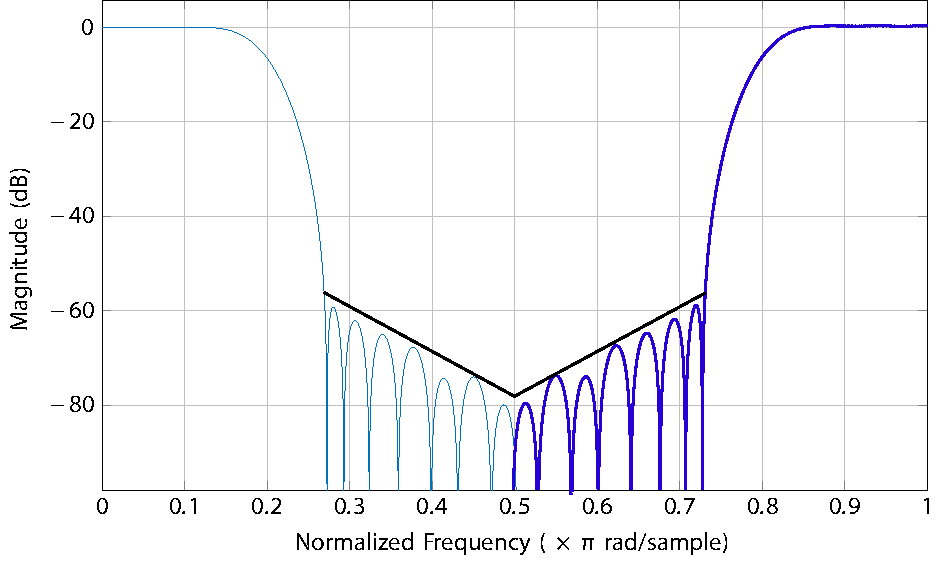
\includegraphics[width=0.7\textwidth]{figures/DecIntCompMirror}
\caption{Decimation filter (blue) with mirrored decimation filter (dark blue)}
\label{fig:MirrorDec}
\end{figure}

From these demands the following specifications should be used for the interpolation filter.

$\omega_{pass}=0.3 \enhed{\pi rad/sample}$\\
$A_{pass}=0 \enhed{dB}$\\
$\omega_{stop}=0.7 \enhed{\pi rad/sample}$\\
$A_{stop}=-60 \enhed{dB}$

A buffer is given to both $\omega_{pass}$ and $\omega_{stop}$ because of quantization, so the following requirements are set for the filter.

$\omega_{pass}=0.4 \enhed{rad/sample}$\\
$A_{pass}=-1 \enhed{dB}$\\
$\omega_{stop}=0.7 \enhed{rad/sample}$\\
$A_{stop}=-80 \enhed{dB}$

If the Kaiser window method is used and the same FIR theory is used as with the decimation filter the following filter is given with quantisized coefficient, see \autoref{fig:IntMag} for magnitude response and \autoref{fig:IntPhase} for phase response. The order of the filter is 34, it is a type 1 FIR filter and has linear phase with a group delay of 17 samples.

\begin{figure}[H]
	\centering
	\tikzsetnextfilename{IntMag}
	% This file was created by matlab2tikz.
%
%The latest updates can be retrieved from
%  http://www.mathworks.com/matlabcentral/fileexchange/22022-matlab2tikz-matlab2tikz
%where you can also make suggestions and rate matlab2tikz.
%
\definecolor{mycolor1}{rgb}{0.00000,0.44700,0.74100}%
%
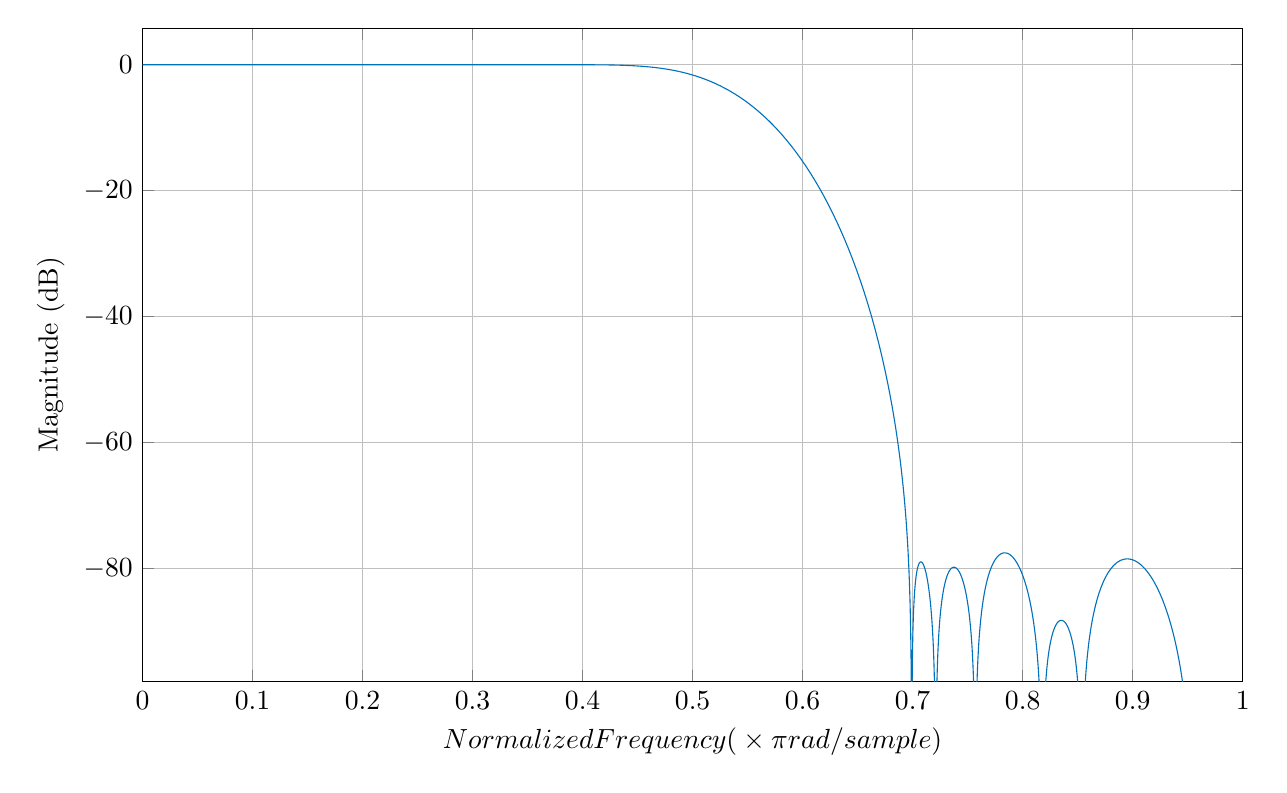
\begin{tikzpicture}

\begin{axis}[%
width=5.5in,
height=3.267in,
at={(1.281in,0.441in)},
scale only axis,
unbounded coords=jump,
xmin=0,
xmax=0.9998779296875,
xlabel={$\text{Normalized Frequency (}\times\pi\text{ rad/sample)}$},
xmajorgrids,
ymin=-97.9178075189385,
ymax=5.80114908390536,
ylabel={Magnitude (dB)},
ymajorgrids,
axis background/.style={fill=white},
]
\addplot [color=mycolor1,solid,forget plot]
  table[row sep=crcr]{%
0	0\\
0.0001220703125	-6.86111434333725e-09\\
0.000244140625	-2.7444059469417e-08\\
0.0003662109375	-6.17477553532808e-08\\
0.00048828125	-1.0977015563185e-07\\
0.0006103515625	-1.71508588664437e-07\\
0.000732421875	-2.46959643845912e-07\\
0.0008544921875	-3.3611900107644e-07\\
0.0009765625	-4.38981658135162e-07\\
0.0010986328125	-5.55541816993355e-07\\
0.001220703125	-6.85792940657848e-07\\
0.0013427734375	-8.2972763948419e-07\\
0.00146484375	-9.87337784863485e-07\\
0.0015869140625	-1.15861456606581e-06\\
0.001708984375	-1.34354831970995e-06\\
0.0018310546875	-1.54212858660685e-06\\
0.001953125	-1.7543442254464e-06\\
0.0020751953125	-1.98018324226723e-06\\
0.002197265625	-2.21963290414351e-06\\
0.0023193359375	-2.47267973918497e-06\\
0.00244140625	-2.73930947969347e-06\\
0.0025634765625	-3.01950706216303e-06\\
0.002685546875	-3.31325679781003e-06\\
0.0028076171875	-3.62054197466932e-06\\
0.0029296875	-3.941345369185e-06\\
0.0030517578125	-4.27564884830645e-06\\
0.003173828125	-4.62343365370543e-06\\
0.0032958984375	-4.98468006071562e-06\\
0.00341796875	-5.35936771939305e-06\\
0.0035400390625	-5.74747559767275e-06\\
0.003662109375	-6.14898169715161e-06\\
0.0037841796875	-6.56386339414894e-06\\
0.00390625	-6.99209732601958e-06\\
0.0040283203125	-7.43365933431051e-06\\
0.004150390625	-7.88852440791743e-06\\
0.0042724609375	-8.35666702414528e-06\\
0.00439453125	-8.83806069396087e-06\\
0.0045166015625	-9.33267824620998e-06\\
0.004638671875	-9.84049177077395e-06\\
0.0047607421875	-1.03614726185697e-05\\
0.0048828125	-1.08955913447062e-05\\
0.0050048828125	-1.14428178790149e-05\\
0.005126953125	-1.20031211849891e-05\\
0.0052490234375	-1.25764697713748e-05\\
0.00537109375	-1.31628311237364e-05\\
0.0054931640625	-1.37621722160475e-05\\
0.005615234375	-1.43744591696304e-05\\
0.0057373046875	-1.49996573668432e-05\\
0.005859375	-1.56377315079226e-05\\
0.0059814453125	-1.62886454972977e-05\\
0.006103515625	-1.69523625572765e-05\\
0.0062255859375	-1.7628845228046e-05\\
0.00634765625	-1.83180551971418e-05\\
0.0064697265625	-1.90199535268221e-05\\
0.006591796875	-1.9734500483537e-05\\
0.0067138671875	-2.04616557084591e-05\\
0.0068359375	-2.12013780469533e-05\\
0.0069580078125	-2.19536256054198e-05\\
0.007080078125	-2.27183558649813e-05\\
0.0072021484375	-2.34955255109526e-05\\
0.00732421875	-2.42850906033709e-05\\
0.0074462890625	-2.50870063496222e-05\\
0.007568359375	-2.59012274455017e-05\\
0.0076904296875	-2.67277076773098e-05\\
0.0078125	-2.75664003197562e-05\\
0.0079345703125	-2.84172578517428e-05\\
0.008056640625	-2.92802319563634e-05\\
0.0081787109375	-3.01552738051214e-05\\
0.00830078125	-3.10423338305554e-05\\
0.0084228515625	-3.19413616693964e-05\\
0.008544921875	-3.28523063330977e-05\\
0.0086669921875	-3.37751162078348e-05\\
0.0087890625	-3.47097388839757e-05\\
0.0089111328125	-3.56561213834539e-05\\
0.009033203125	-3.66142099323952e-05\\
0.0091552734375	-3.75839501884911e-05\\
0.00927734375	-3.85652871273123e-05\\
0.0093994140625	-3.95581649286214e-05\\
0.009521484375	-4.05625272037469e-05\\
0.0096435546875	-4.15783169387396e-05\\
0.009765625	-4.2605476380686e-05\\
0.0098876953125	-4.3643947151395e-05\\
0.010009765625	-4.46936701905543e-05\\
0.0101318359375	-4.57545858125741e-05\\
0.01025390625	-4.6826633706587e-05\\
0.0103759765625	-4.79097527659178e-05\\
0.010498046875	-4.90038814291438e-05\\
0.0106201171875	-5.01089574527214e-05\\
0.0107421875	-5.1224917797299e-05\\
0.0108642578125	-5.23516989687778e-05\\
0.010986328125	-5.34892367909379e-05\\
0.0111083984375	-5.46374663485949e-05\\
0.01123046875	-5.57963223286606e-05\\
0.0113525390625	-5.69657385653954e-05\\
0.011474609375	-5.81456483246257e-05\\
0.0115966796875	-5.93359844174302e-05\\
0.01171875	-6.053667885908e-05\\
0.0118408203125	-6.17476630395686e-05\\
0.011962890625	-6.2968867894142e-05\\
0.0120849609375	-6.42002236759254e-05\\
0.01220703125	-6.54416600127661e-05\\
0.0123291015625	-6.66931059640774e-05\\
0.012451171875	-6.7954489963995e-05\\
0.0125732421875	-6.92257399350638e-05\\
0.0126953125	-7.05067830608641e-05\\
0.0128173828125	-7.1797546183916e-05\\
0.012939453125	-7.3097955294088e-05\\
0.0130615234375	-7.44079359265015e-05\\
0.01318359375	-7.57274131615304e-05\\
0.0133056640625	-7.70563113405842e-05\\
0.013427734375	-7.83945542934816e-05\\
0.0135498046875	-7.97420652816072e-05\\
0.013671875	-8.10987669979113e-05\\
0.0137939453125	-8.24645816805969e-05\\
0.013916015625	-8.3839430885746e-05\\
0.0140380859375	-8.52232356578497e-05\\
0.01416015625	-8.66159165298086e-05\\
0.0142822265625	-8.80173935229323e-05\\
0.014404296875	-8.94275860332527e-05\\
0.0145263671875	-9.08464130020548e-05\\
0.0146484375	-9.22737928021888e-05\\
0.0147705078125	-9.37096433517581e-05\\
0.014892578125	-9.51538818867448e-05\\
0.0150146484375	-9.66064253020704e-05\\
0.01513671875	-9.80671899242225e-05\\
0.0152587890625	-9.95360915112542e-05\\
0.015380859375	-0.000101013045423315\\
0.0155029296875	-0.00010249796645212\\
0.015625	-0.000103990768877793\\
0.0157470703125	-0.000105491366582555\\
0.015869140625	-0.000106999672823349\\
0.0159912109375	-0.0001085156005729\\
0.01611328125	-0.00011003906206497\\
0.0162353515625	-0.000111569969249103\\
0.016357421875	-0.000113108233620096\\
0.0164794921875	-0.000114653766047468\\
0.0166015625	-0.000116206477116521\\
0.0167236328125	-0.000117766276844122\\
0.016845703125	-0.000119333074792394\\
0.0169677734375	-0.000120906780182395\\
0.01708984375	-0.000122487301609908\\
0.0172119140625	-0.000124074547443342\\
0.017333984375	-0.000125668425482672\\
0.0174560546875	-0.000127268843129968\\
0.017578125	-0.000128875707275711\\
0.0177001953125	-0.000130488924639849\\
0.017822265625	-0.000132108401203368\\
0.0179443359375	-0.000133734042776723\\
0.01806640625	-0.000135365754658778\\
0.0181884765625	-0.000137003441750494\\
0.018310546875	-0.000138647008554926\\
0.0184326171875	-0.000140296359234071\\
0.0185546875	-0.00014195139755202\\
0.0186767578125	-0.000143612026761275\\
0.018798828125	-0.000145278149943806\\
0.0189208984375	-0.00014694966961315\\
0.01904296875	-0.000148626487998627\\
0.0191650390625	-0.000150308507045338\\
0.019287109375	-0.000151995628129953\\
0.0194091796875	-0.000153687752515452\\
0.01953125	-0.000155384780953227\\
0.0196533203125	-0.000157086613853608\\
0.019775390625	-0.00015879315139955\\
0.0198974609375	-0.00016050429326242\\
0.02001953125	-0.000162219938999897\\
0.0201416015625	-0.000163939987658068\\
0.020263671875	-0.000165664338055649\\
0.0203857421875	-0.000167392888670292\\
0.0205078125	-0.000169125537638593\\
0.0206298828125	-0.000170862182869769\\
0.020751953125	-0.000172602721875137\\
0.0208740234375	-0.000174347051938639\\
0.02099609375	-0.000176095070003157\\
0.0211181640625	-0.000177846672784199\\
0.021240234375	-0.000179601756713055\\
0.0213623046875	-0.000181360217823112\\
0.021484375	-0.000183121952034071\\
0.0216064453125	-0.000184886854981414\\
0.021728515625	-0.000186654821902721\\
0.0218505859375	-0.000188425747921883\\
0.02197265625	-0.000190199527878576\\
0.0220947265625	-0.000191976056271415\\
0.022216796875	-0.000193755227485326\\
0.0223388671875	-0.000195536935677865\\
0.0224609375	-0.000197321074608681\\
0.0225830078125	-0.000199107538037424\\
0.022705078125	-0.000200896219268998\\
0.0228271484375	-0.000202687011665148\\
0.02294921875	-0.00020447980807603\\
0.0230712890625	-0.000206274501465487\\
0.023193359375	-0.000208070984285769\\
0.0233154296875	-0.000209869148989128\\
0.0234375	-0.000211668887857286\\
0.0235595703125	-0.000213470092887746\\
0.023681640625	-0.000215272655964327\\
0.0238037109375	-0.000217076468686628\\
0.02392578125	-0.000218881422711092\\
0.0240478515625	-0.000220687409296261\\
0.024169921875	-0.000222494319757516\\
0.0242919921875	-0.000224302045012337\\
0.0244140625	-0.00022611047609189\\
0.0245361328125	-0.00022791950368628\\
0.024658203125	-0.000229729018485614\\
0.0247802734375	-0.000231538910952622\\
0.02490234375	-0.000233349071550037\\
0.0250244140625	-0.000235159390456374\\
0.025146484375	-0.000236969757850147\\
0.0252685546875	-0.000238780063796185\\
0.025390625	-0.000240590198245627\\
0.0255126953125	-0.000242400051035929\\
0.025634765625	-0.000244209511947702\\
0.0257568359375	-0.000246018470591025\\
0.02587890625	-0.00024782681657598\\
0.0260009765625	-0.000249634439455804\\
0.026123046875	-0.000251441228670046\\
0.0262451171875	-0.000253247073601415\\
0.0263671875	-0.000255051863575773\\
0.0264892578125	-0.000256855487918983\\
0.026611328125	-0.000258657835729537\\
0.0267333984375	-0.000260458796276453\\
0.02685546875	-0.000262258258715065\\
0.0269775390625	-0.000264056112200706\\
0.027099609375	-0.000265852245718179\\
0.0272216796875	-0.000267646548422817\\
0.02734375	-0.000269438909356268\\
0.0274658203125	-0.000271229217617019\\
0.027587890625	-0.000273017362133032\\
0.0277099609375	-0.000274803232116483\\
0.02783203125	-0.000276586716495331\\
0.0279541015625	-0.000278367704368065\\
0.028076171875	-0.000280146084890021\\
0.0281982421875	-0.000281921747159686\\
0.0283203125	-0.000283694580275551\\
0.0284423828125	-0.000285464473449792\\
0.028564453125	-0.000287231315951431\\
0.0286865234375	-0.000288994996992642\\
0.02880859375	-0.00029075540589929\\
0.0289306640625	-0.000292512432110925\\
0.029052734375	-0.000294265965010254\\
0.0291748046875	-0.000296015894150514\\
0.029296875	-0.000297762109084942\\
0.0294189453125	-0.000299504499480463\\
0.029541015625	-0.00030124295517453\\
0.0296630859375	-0.000302977365947754\\
0.02978515625	-0.000304707621694433\\
0.0299072265625	-0.000306433612593082\\
0.030029296875	-0.000308155228651685\\
0.0301513671875	-0.000309872360276131\\
0.0302734375	-0.000311584897701778\\
0.0303955078125	-0.000313292731561887\\
0.030517578125	-0.000314995752432878\\
0.0306396484375	-0.000316693851118544\\
0.03076171875	-0.000318386918479519\\
0.0308837890625	-0.000320074845660656\\
0.031005859375	-0.000321757523749966\\
0.0311279296875	-0.000323434844290205\\
0.03125	-0.000325106698653599\\
0.0313720703125	-0.000326772978610279\\
0.031494140625	-0.000328433576044063\\
0.0316162109375	-0.000330088383009297\\
0.03173828125	-0.00033173729173086\\
0.0318603515625	-0.00033338019460416\\
0.031982421875	-0.000335016984308822\\
0.0321044921875	-0.000336647553638159\\
0.0322265625	-0.000338271795612854\\
0.0323486328125	-0.00033988960348097\\
0.032470703125	-0.000341500870717937\\
0.0325927734375	-0.000343105491026563\\
0.03271484375	-0.000344703358280185\\
0.0328369140625	-0.000346294366636357\\
0.032958984375	-0.000347878410480007\\
0.0330810546875	-0.000349455384423436\\
0.033203125	-0.000351025183363163\\
0.0333251953125	-0.000352587702423079\\
0.033447265625	-0.000354142836954452\\
0.0335693359375	-0.00035569048270645\\
0.03369140625	-0.00035723053554193\\
0.0338134765625	-0.00035876289166481\\
0.033935546875	-0.000360287447563223\\
0.0340576171875	-0.000361804100009522\\
0.0341796875	-0.000363312746117117\\
0.0343017578125	-0.000364813283226795\\
0.034423828125	-0.000366305608963557\\
0.0345458984375	-0.000367789621293468\\
0.03466796875	-0.000369265218580495\\
0.0347900390625	-0.000370732299359133\\
0.034912109375	-0.000372190762561786\\
0.0350341796875	-0.000373640507518758\\
0.03515625	-0.000375081433730884\\
0.0352783203125	-0.000376513441153747\\
0.035400390625	-0.000377936430083992\\
0.0355224609375	-0.00037935030115932\\
0.03564453125	-0.000380754955301654\\
0.0357666015625	-0.000382150293887662\\
0.035888671875	-0.000383536218635072\\
0.0360107421875	-0.000384912631602674\\
0.0361328125	-0.000386279435190318\\
0.0362548828125	-0.000387636532309443\\
0.036376953125	-0.000388983826098865\\
0.0364990234375	-0.000390321220265832\\
0.03662109375	-0.000391648618688123\\
0.0367431640625	-0.00039296592581195\\
0.036865234375	-0.00039427304648143\\
0.0369873046875	-0.000395569885824898\\
0.037109375	-0.000396856349595964\\
0.0372314453125	-0.000398132343718771\\
0.037353515625	-0.000399397774742738\\
0.0374755859375	-0.000400652549501501\\
0.03759765625	-0.000401896575453975\\
0.0377197265625	-0.000403129760286447\\
0.037841796875	-0.000404352012196796\\
0.0379638671875	-0.000405563239951334\\
0.0380859375	-0.000406763352600592\\
0.0382080078125	-0.000407952259820377\\
0.038330078125	-0.000409129871513869\\
0.0384521484375	-0.000410296098323215\\
0.03857421875	-0.000411450851174777\\
0.0386962890625	-0.000412594041563352\\
0.038818359375	-0.000413725581438484\\
0.0389404296875	-0.000414845383261309\\
0.0390625	-0.000415953359890864\\
0.0391845703125	-0.000417049424811466\\
0.039306640625	-0.000418133491905337\\
0.0394287109375	-0.00041920547562313\\
0.03955078125	-0.000420265290927091\\
0.0396728515625	-0.000421312853291056\\
0.039794921875	-0.000422348078643608\\
0.0399169921875	-0.000423370883481766\\
0.0400390625	-0.000424381184870981\\
0.0401611328125	-0.000425378900331452\\
0.040283203125	-0.000426363948008657\\
0.0404052734375	-0.000427336246502819\\
0.04052734375	-0.00042829571503944\\
0.0406494140625	-0.000429242273298769\\
0.040771484375	-0.000430175841586333\\
0.0408935546875	-0.000431096340832937\\
0.041015625	-0.000432003692310445\\
0.0411376953125	-0.000432897818086531\\
0.041259765625	-0.000433778640683613\\
0.0413818359375	-0.000434646083306234\\
0.04150390625	-0.000435500069499994\\
0.0416259765625	-0.000436340523719991\\
0.041748046875	-0.000437167370762381\\
0.0418701171875	-0.000437980536105442\\
0.0419921875	-0.000438779945795886\\
0.0421142578125	-0.000439565526562546\\
0.042236328125	-0.00044033720570269\\
0.0423583984375	-0.000441094910968332\\
0.04248046875	-0.000441838570964137\\
0.0426025390625	-0.000442568114806363\\
0.042724609375	-0.000443283472122857\\
0.0428466796875	-0.000443984573394118\\
0.04296875	-0.000444671349555392\\
0.0430908203125	-0.000445343732224046\\
0.043212890625	-0.000446001653642725\\
0.0433349609375	-0.000446645046736194\\
0.04345703125	-0.000447273844997653\\
0.0435791015625	-0.000447887982659267\\
0.043701171875	-0.000448487394521635\\
0.0438232421875	-0.000449072016124319\\
0.0439453125	-0.000449641783575316\\
0.0440673828125	-0.000450196633664746\\
0.044189453125	-0.000450736503921689\\
0.0443115234375	-0.000451261332500508\\
0.04443359375	-0.000451771058123995\\
0.0445556640625	-0.000452265620424441\\
0.044677734375	-0.000452744959488882\\
0.0447998046875	-0.000453209016143319\\
0.044921875	-0.000453657732066404\\
0.0450439453125	-0.000454091049391536\\
0.045166015625	-0.000454508911047924\\
0.0452880859375	-0.000454911260703739\\
0.04541015625	-0.00045529804265243\\
0.0455322265625	-0.000455669201983255\\
0.045654296875	-0.000456024684353906\\
0.0457763671875	-0.000456364436217882\\
0.0458984375	-0.000456688404767647\\
0.0460205078125	-0.000456996537877785\\
0.046142578125	-0.000457288784161847\\
0.0462646484375	-0.000457565092858658\\
0.04638671875	-0.000457825414116542\\
0.0465087890625	-0.000458069698595409\\
0.046630859375	-0.000458297897864668\\
0.0467529296875	-0.000458509964119003\\
0.046875	-0.00045870585040575\\
0.0469970703125	-0.000458885510340679\\
0.047119140625	-0.000459048898505898\\
0.0472412109375	-0.000459195969938264\\
0.04736328125	-0.000459326680754657\\
0.0474853515625	-0.000459440987526705\\
0.047607421875	-0.00045953884773553\\
0.0477294921875	-0.000459620219658063\\
0.0478515625	-0.000459685062253357\\
0.0479736328125	-0.000459733335219426\\
0.048095703125	-0.000459764999050094\\
0.0482177734375	-0.000459780015034994\\
0.04833984375	-0.000459778345202722\\
0.0484619140625	-0.000459759952320837\\
0.048583984375	-0.000459724800066397\\
0.0487060546875	-0.000459672852741733\\
0.048828125	-0.000459604075444986\\
0.0489501953125	-0.000459518434183792\\
0.049072265625	-0.000459415895647908\\
0.0491943359375	-0.000459296427266054\\
0.04931640625	-0.000459159997319603\\
0.0494384765625	-0.000459006574999421\\
0.049560546875	-0.000458836130007967\\
0.0496826171875	-0.000458648633127723\\
0.0498046875	-0.000458444055766449\\
0.0499267578125	-0.000458222370127714\\
0.050048828125	-0.000457983549381424\\
0.0501708984375	-0.000457727567322763\\
0.05029296875	-0.000457454398599566\\
0.0504150390625	-0.000457164018712319\\
0.050537109375	-0.000456856403957318\\
0.0506591796875	-0.000456531531426663\\
0.05078125	-0.000456189378951422\\
0.0509033203125	-0.000455829925328999\\
0.051025390625	-0.000455453150095764\\
0.0511474609375	-0.000455059033583893\\
0.05126953125	-0.000454647556978216\\
0.0513916015625	-0.000454218702259368\\
0.051513671875	-0.000453772452260637\\
0.0516357421875	-0.000453308790611118\\
0.0517578125	-0.000452827701792557\\
0.0518798828125	-0.000452329171082511\\
0.052001953125	-0.000451813184611183\\
0.0521240234375	-0.000451279729304588\\
0.05224609375	-0.000450728793055077\\
0.0523681640625	-0.000450160364380281\\
0.052490234375	-0.000449574432764166\\
0.0526123046875	-0.000448970988486508\\
0.052734375	-0.000448350022679733\\
0.0528564453125	-0.00044771152732892\\
0.052978515625	-0.000447055495214954\\
0.0531005859375	-0.000446381919971373\\
0.05322265625	-0.000445690796141207\\
0.0533447265625	-0.000444982118949611\\
0.053466796875	-0.000444255884701761\\
0.0535888671875	-0.00044351209027127\\
0.0537109375	-0.000442750733554931\\
0.0538330078125	-0.000441971813302189\\
0.053955078125	-0.000441175329058296\\
0.0540771484375	-0.000440361281221158\\
0.05419921875	-0.000439529670984484\\
0.0543212890625	-0.000438680500508326\\
0.054443359375	-0.000437813772691698\\
0.0545654296875	-0.000436929491399951\\
0.0546875	-0.00043602766118056\\
0.0548095703125	-0.00043510828760418\\
0.054931640625	-0.00043417137698043\\
0.0550537109375	-0.000433216936585268\\
0.05517578125	-0.000432244974376772\\
0.0552978515625	-0.000431255499336203\\
0.055419921875	-0.000430248521183785\\
0.0555419921875	-0.000429224050549237\\
0.0556640625	-0.000428182098914931\\
0.0557861328125	-0.000427122678615888\\
0.055908203125	-0.000426045802782937\\
0.0560302734375	-0.000424951485513247\\
0.05615234375	-0.000423839741642951\\
0.0562744140625	-0.000422710586974517\\
0.056396484375	-0.000421564038049382\\
0.0565185546875	-0.000420400112375319\\
0.056640625	-0.000419218828255907\\
0.0567626953125	-0.000418020204790537\\
0.056884765625	-0.000416804262101778\\
0.0570068359375	-0.000415571020994321\\
0.05712890625	-0.000414320503239196\\
0.0572509765625	-0.000413052731403241\\
0.057373046875	-0.000411767728905943\\
0.0574951171875	-0.000410465520076286\\
0.0576171875	-0.000409146130039062\\
0.0577392578125	-0.000407809584828556\\
0.057861328125	-0.000406455911218018\\
0.0579833984375	-0.00040508513700388\\
0.05810546875	-0.000403697290721539\\
0.0582275390625	-0.000402292401702198\\
0.058349609375	-0.000400870500300243\\
0.0584716796875	-0.000399431617609025\\
0.05859375	-0.000397975785574545\\
0.0587158203125	-0.000396503036938611\\
0.058837890625	-0.000395013405466216\\
0.0589599609375	-0.000393506925547626\\
0.05908203125	-0.000391983632596293\\
0.0592041015625	-0.000390443562821474\\
0.059326171875	-0.000388886753228235\\
0.0594482421875	-0.000387313241731135\\
0.0595703125	-0.000385723066983701\\
0.0596923828125	-0.000384116268605794\\
0.059814453125	-0.000382492887013086\\
0.0599365234375	-0.000380852963417055\\
0.06005859375	-0.000379196539938675\\
0.0601806640625	-0.000377523659494727\\
0.060302734375	-0.000375834365740957\\
0.0604248046875	-0.000374128703413135\\
0.060546875	-0.000372406717872309\\
0.0606689453125	-0.000370668455389023\\
0.060791015625	-0.000368913963029627\\
0.0609130859375	-0.000367143288713123\\
0.06103515625	-0.000365356481211165\\
0.0611572265625	-0.000363553590034371\\
0.061279296875	-0.000361734665659696\\
0.0614013671875	-0.000359899759246218\\
0.0615234375	-0.000358048922862508\\
0.0616455078125	-0.000356182209372946\\
0.061767578125	-0.000354299672494562\\
0.0618896484375	-0.000352401366626509\\
0.06201171875	-0.000350487347134276\\
0.0621337890625	-0.000348557670122318\\
0.062255859375	-0.00034661239254774\\
0.0623779296875	-0.000344651572106613\\
0.0625	-0.000342675267461345\\
0.0626220703125	-0.000340683537842779\\
0.062744140625	-0.000338676443504937\\
0.0628662109375	-0.000336654045383966\\
0.06298828125	-0.000334616405154975\\
0.0631103515625	-0.000332563585516255\\
0.063232421875	-0.00033049564973453\\
0.0633544921875	-0.000328412661986022\\
0.0634765625	-0.000326314687185914\\
0.0635986328125	-0.000324201791045198\\
0.063720703125	-0.000322074040127518\\
0.0638427734375	-0.000319931501735482\\
0.06396484375	-0.000317774243910662\\
0.0640869140625	-0.000315602335490439\\
0.064208984375	-0.000313415846108001\\
0.0643310546875	-0.000311214846249186\\
0.064453125	-0.000308999407025112\\
0.0645751953125	-0.000306769600342705\\
0.064697265625	-0.000304525499018382\\
0.0648193359375	-0.000302267176493842\\
0.06494140625	-0.000299994706949747\\
0.0650634765625	-0.000297708165476251\\
0.065185546875	-0.000295407627788791\\
0.0653076171875	-0.000293093170341763\\
0.0654296875	-0.000290764870499061\\
0.0655517578125	-0.000288422806136168\\
0.065673828125	-0.000286067056094907\\
0.0657958984375	-0.000283697699842378\\
0.06591796875	-0.000281314817584644\\
0.0660400390625	-0.000278918490323576\\
0.066162109375	-0.000276508799743169\\
0.0662841796875	-0.000274085828266379\\
0.06640625	-0.000271649659055129\\
0.0665283203125	-0.00026920037595346\\
0.066650390625	-0.000266738063544381\\
0.0667724609375	-0.000264262807263549\\
0.06689453125	-0.000261774692944527\\
0.0670166015625	-0.000259273807500904\\
0.067138671875	-0.000256760238301013\\
0.0672607421875	-0.000254234073452153\\
0.0673828125	-0.000251695401857432\\
0.0675048828125	-0.000249144313045235\\
0.067626953125	-0.000246580897282911\\
0.0677490234375	-0.000244005245463086\\
0.06787109375	-0.000241417449217352\\
0.0679931640625	-0.000238817600802577\\
0.068115234375	-0.000236205793271438\\
0.0682373046875	-0.000233582120188203\\
0.068359375	-0.00023094667596979\\
0.0684814453125	-0.000228299555544709\\
0.068603515625	-0.000225640854580433\\
0.0687255859375	-0.000222970669426559\\
0.06884765625	-0.000220289097057957\\
0.0689697265625	-0.000217596235017936\\
0.069091796875	-0.000214892181702453\\
0.0692138671875	-0.000212177036019057\\
0.0693359375	-0.00020945089744373\\
0.0694580078125	-0.000206713866248265\\
0.069580078125	-0.000203966043272885\\
0.0697021484375	-0.000201207529926251\\
0.06982421875	-0.000198438428412828\\
0.0699462890625	-0.000195658841334989\\
0.070068359375	-0.000192868872090912\\
0.0701904296875	-0.000190068624590367\\
0.0703125	-0.000187258203425245\\
0.0704345703125	-0.000184437713755869\\
0.070556640625	-0.000181607261311001\\
0.0706787109375	-0.000178766952444676\\
0.07080078125	-0.000175916894136208\\
0.0709228515625	-0.000173057193933346\\
0.071044921875	-0.000170187959895429\\
0.0711669921875	-0.000167309300763918\\
0.0712890625	-0.000164421325848707\\
0.0714111328125	-0.000161524144971281\\
0.071533203125	-0.00015861786852156\\
0.0716552734375	-0.000155702607457897\\
0.07177734375	-0.000152778473363924\\
0.0718994140625	-0.000149845578334862\\
0.072021484375	-0.000146904034920681\\
0.0721435546875	-0.000143953956353471\\
0.072265625	-0.000140995456376913\\
0.0723876953125	-0.000138028649189437\\
0.072509765625	-0.000135053649557904\\
0.0726318359375	-0.000132070572817611\\
0.07275390625	-0.000129079534758603\\
0.0728759765625	-0.000126080651739358\\
0.072998046875	-0.000123074040573101\\
0.0731201171875	-0.000120059818698337\\
0.0732421875	-0.000117038103837785\\
0.0733642578125	-0.000114009014453131\\
0.073486328125	-0.00011097266934712\\
0.0736083984375	-0.000107929187834088\\
0.07373046875	-0.000104878689683119\\
0.0738525390625	-0.000101821295288573\\
0.073974609375	-9.87571252721864e-05\\
0.0740966796875	-9.56863009378139e-05\\
0.07421875	-9.26089439303723e-05\\
0.0743408203125	-8.95251763495253e-05\\
0.074462890625	-8.64351209202141e-05\\
0.0745849609375	-8.3338900481067e-05\\
0.07470703125	-8.02366386665199e-05\\
0.0748291015625	-7.71284592815391e-05\\
0.074951171875	-7.40144867563686e-05\\
0.0750732421875	-7.08948457486258e-05\\
0.0751953125	-6.77696614843626e-05\\
0.0753173828125	-6.46390595875346e-05\\
0.075439453125	-6.1503166023158e-05\\
0.0755615234375	-5.83621072109963e-05\\
0.07568359375	-5.52160100255605e-05\\
0.0758056640625	-5.20650015118918e-05\\
0.075927734375	-4.89092093971522e-05\\
0.0760498046875	-4.57487616358776e-05\\
0.076171875	-4.25837865236645e-05\\
0.0762939453125	-3.9414412754013e-05\\
0.076416015625	-3.6240769475171e-05\\
0.0765380859375	-3.30629861764464e-05\\
0.07666015625	-2.98811925176778e-05\\
0.0767822265625	-2.66955187839812e-05\\
0.076904296875	-2.35060953741595e-05\\
0.0770263671875	-2.03130531417628e-05\\
0.0771484375	-1.71165232814019e-05\\
0.0772705078125	-1.39166372150612e-05\\
0.077392578125	-1.07135268763159e-05\\
0.0775146484375	-7.50732425558454e-06\\
0.07763671875	-4.29816191171994e-06\\
0.0777587890625	-1.08617251726173e-06\\
0.077880859375	2.12851091418997e-06\\
0.0780029296875	5.34575491428768e-06\\
0.078125	8.56542601468391e-06\\
0.0782470703125	1.17873902354404e-05\\
0.078369140625	1.50115134260886e-05\\
0.0784912109375	1.82376610950996e-05\\
0.07861328125	2.1465698580414e-05\\
0.0787353515625	2.46954908220687e-05\\
0.078857421875	2.79269027032569e-05\\
0.0789794921875	3.11597987092682e-05\\
0.0791015625	3.43940430980183e-05\\
0.0792236328125	3.76294999568927e-05\\
0.079345703125	4.08660330890598e-05\\
0.0794677734375	4.41035061271577e-05\\
0.07958984375	4.73417823627642e-05\\
0.0797119140625	5.05807250874568e-05\\
0.079833984375	5.38201971949093e-05\\
0.0799560546875	5.70600614651084e-05\\
0.080078125	6.03001804506675e-05\\
0.0802001953125	6.35404165905129e-05\\
0.080322265625	6.67806320393538e-05\\
0.0804443359375	7.00206888382127e-05\\
0.08056640625	7.32604488007382e-05\\
0.0806884765625	7.64997737405793e-05\\
0.080810546875	7.97385250734806e-05\\
0.0809326171875	8.29765642720304e-05\\
0.0810546875	8.62137524677564e-05\\
0.0811767578125	8.94499509058733e-05\\
0.081298828125	9.26850204336915e-05\\
0.0814208984375	9.59188219553653e-05\\
0.08154296875	9.91512161476749e-05\\
0.0816650390625	0.000102382063687401\\
0.081787109375	0.000105611225023949\\
0.0819091796875	0.000108838560493041\\
0.08203125	0.000112063930487238\\
0.0821533203125	0.000115287195228575\\
0.082275390625	0.00011850821471171\\
0.0823974609375	0.000121726849101833\\
0.08251953125	0.00012494295833676\\
0.0826416015625	0.000128156402354307\\
0.082763671875	0.000131367040921759\\
0.0828857421875	0.00013457473392009\\
0.0830078125	0.000137779341059741\\
0.0831298828125	0.000140980722107997\\
0.083251953125	0.000144178736604772\\
0.0833740234375	0.000147373244374194\\
0.08349609375	0.000150564104899331\\
0.0836181640625	0.000153751177833783\\
0.083740234375	0.000156934322774305\\
0.0838623046875	0.000160113399374495\\
0.083984375	0.000163288267174266\\
0.0841064453125	0.000166458785770374\\
0.084228515625	0.000169624814873259\\
0.0843505859375	0.000172786214022835\\
0.08447265625	0.000175942842986387\\
0.0845947265625	0.000179094561417514\\
0.084716796875	0.000182241229083502\\
0.0848388671875	0.000185382705808479\\
0.0849609375	0.000188518851416575\\
0.0850830078125	0.000191649525788762\\
0.085205078125	0.000194774588976543\\
0.0853271484375	0.000197893900974577\\
0.08544921875	0.000201007321948055\\
0.0855712890625	0.000204114712062164\\
0.085693359375	0.000207215931652627\\
0.0858154296875	0.000210310841168848\\
0.0859375	0.000213399301060235\\
0.0860595703125	0.000216481171946725\\
0.086181640625	0.000219556314561942\\
0.0863037109375	0.000222624589753195\\
0.08642578125	0.000225685858538327\\
0.0865478515625	0.000228739982048864\\
0.086669921875	0.000231786821473179\\
0.0867919921875	0.000234826238283858\\
0.0869140625	0.000237858094067178\\
0.0870361328125	0.000240882250466257\\
0.087158203125	0.000243898569465273\\
0.0872802734375	0.000246906913048406\\
0.08740234375	0.000249907143540895\\
0.0875244140625	0.000252899123324823\\
0.087646484375	0.000255882714952804\\
0.0877685546875	0.000258857781375355\\
0.087890625	0.000261824185599835\\
0.0880126953125	0.000264781790747293\\
0.088134765625	0.000267730460393523\\
0.0882568359375	0.000270670058171163\\
0.08837890625	0.000273600447997069\\
0.0885009765625	0.000276521494015469\\
0.088623046875	0.000279433060597967\\
0.0887451171875	0.000282335012343538\\
0.0888671875	0.000285227214192219\\
0.0889892578125	0.00028810953131142\\
0.089111328125	0.000290981829095927\\
0.0892333984375	0.000293843973167895\\
0.08935546875	0.000296695829604232\\
0.0894775390625	0.000299537264538685\\
0.089599609375	0.000302368144616594\\
0.0897216796875	0.000305188336710671\\
0.08984375	0.00030799770786416\\
0.0899658203125	0.000310796125575052\\
0.090087890625	0.000313583457625555\\
0.0902099609375	0.000316359572082092\\
0.09033203125	0.000319124337465837\\
0.0904541015625	0.000321877622468492\\
0.090576171875	0.000324619296179662\\
0.0906982421875	0.000327349228030016\\
0.0908203125	0.000330067287904967\\
0.0909423828125	0.000332773345974147\\
0.091064453125	0.00033546727263456\\
0.0911865234375	0.000338148938908489\\
0.09130859375	0.000340818215988747\\
0.0914306640625	0.000343474975636582\\
0.091552734375	0.000346119089840613\\
0.0916748046875	0.000348750430987366\\
0.091796875	0.000351368872031799\\
0.0919189453125	0.000353974286213088\\
0.092041015625	0.00035656654711147\\
0.0921630859375	0.000359145528875615\\
0.09228515625	0.000361711106052098\\
0.0924072265625	0.000364263153528555\\
0.092529296875	0.00036680154670421\\
0.0926513671875	0.000369326161376193\\
0.0927734375	0.00037183687391007\\
0.0928955078125	0.00037433356095562\\
0.093017578125	0.000376816099674215\\
0.0931396484375	0.000379284367795663\\
0.09326171875	0.000381738243390828\\
0.0933837890625	0.000384177605155855\\
0.093505859375	0.000386602332071107\\
0.0936279296875	0.00038901230374222\\
0.09375	0.000391407400343269\\
0.0938720703125	0.000393787502332543\\
0.093994140625	0.000396152490793611\\
0.0941162109375	0.000398502247435317\\
0.09423828125	0.000400836654250725\\
0.0943603515625	0.00040315559397186\\
0.094482421875	0.000405458949671811\\
0.0946044921875	0.000407746605162629\\
0.0947265625	0.000410018444597426\\
0.0948486328125	0.000412274352811437\\
0.094970703125	0.000414514215094641\\
0.0950927734375	0.000416737917475984\\
0.09521484375	0.000418945346268629\\
0.0953369140625	0.000421136388581544\\
0.095458984375	0.000423310932035292\\
0.0955810546875	0.000425468864762024\\
0.095703125	0.000427610075519169\\
0.0958251953125	0.000429734453746278\\
0.095947265625	0.000431841889394491\\
0.0960693359375	0.00043393227292654\\
0.09619140625	0.000436005495544123\\
0.0963134765625	0.000438061449074212\\
0.096435546875	0.000440100025912216\\
0.0965576171875	0.000442121118965133\\
0.0966796875	0.000444124621992614\\
0.0968017578125	0.000446110429209057\\
0.096923828125	0.000448078435567822\\
0.0970458984375	0.000450028536533864\\
0.09716796875	0.000451960628424786\\
0.0972900390625	0.000453874608069782\\
0.097412109375	0.000455770372923325\\
0.0975341796875	0.000457647821178853\\
0.09765625	0.000459506851768765\\
0.0977783203125	0.000461347364137055\\
0.097900390625	0.000463169258523521\\
0.0980224609375	0.000464972435793243\\
0.09814453125	0.000466756797493417\\
0.0982666015625	0.000468522245967051\\
0.098388671875	0.000470268684125585\\
0.0985107421875	0.000471996015619425\\
0.0986328125	0.000473704144837939\\
0.0987548828125	0.000475392976909461\\
0.098876953125	0.000477062417644447\\
0.0989990234375	0.000478712373535473\\
0.09912109375	0.000480342751814078\\
0.0992431640625	0.000481953460564455\\
0.099365234375	0.000483544408439229\\
0.0994873046875	0.000485115504886835\\
0.099609375	0.000486666660208357\\
0.0997314453125	0.000488197785273314\\
0.099853515625	0.000489708791917565\\
0.0999755859375	0.000491199592488556\\
0.10009765625	0.000492670100300074\\
0.1002197265625	0.000494120229348027\\
0.100341796875	0.00049554989442413\\
0.1004638671875	0.000496959011115905\\
0.1005859375	0.000498347495692997\\
0.1007080078125	0.000499715265391387\\
0.100830078125	0.000501062238015493\\
0.1009521484375	0.000502388332336068\\
0.10107421875	0.000503693467862831\\
0.1011962890625	0.000504977564958153\\
0.101318359375	0.000506240544666525\\
0.1014404296875	0.000507482328998776\\
0.1015625	0.000508702840591013\\
0.1016845703125	0.000509902003159368\\
0.101806640625	0.000511079740988407\\
0.1019287109375	0.000512235979385878\\
0.10205078125	0.000513370644341649\\
0.1021728515625	0.000514483662755083\\
0.102294921875	0.000515574962321352\\
0.1024169921875	0.000516644471701966\\
0.1025390625	0.000517692120240554\\
0.1026611328125	0.000518717838303928\\
0.102783203125	0.000519721556884178\\
0.1029052734375	0.000520703208053419\\
0.10302734375	0.000521662724622729\\
0.1031494140625	0.000522600040312682\\
0.103271484375	0.000523515089696502\\
0.1033935546875	0.000524407808313754\\
0.103515625	0.000525278132329277\\
0.1036376953125	0.000526125999101623\\
0.103759765625	0.000526951346671467\\
0.1038818359375	0.00052775411404582\\
0.10400390625	0.000528534241084344\\
0.1041259765625	0.000529291668499354\\
0.104248046875	0.000530026338026346\\
0.1043701171875	0.000530738192253466\\
0.1044921875	0.000531427174564669\\
0.1046142578125	0.000532093229367092\\
0.104736328125	0.000532736301977366\\
0.1048583984375	0.000533356338564772\\
0.10498046875	0.000533953286264932\\
0.1051025390625	0.000534527093122961\\
0.105224609375	0.000535077708093468\\
0.1053466796875	0.000535605081040558\\
0.10546875	0.000536109162851517\\
0.1055908203125	0.000536589905152596\\
0.105712890625	0.000537047260706913\\
0.1058349609375	0.000537481183073396\\
0.10595703125	0.000537891626890996\\
0.1060791015625	0.000538278547594473\\
0.106201171875	0.000538641901698611\\
0.1063232421875	0.000538981646514003\\
0.1064453125	0.000539297740374423\\
0.1065673828125	0.000539590142693669\\
0.106689453125	0.000539858813681349\\
0.1068115234375	0.000540103714513407\\
0.10693359375	0.00054032480738897\\
0.1070556640625	0.000540522055416659\\
0.107177734375	0.000540695422728277\\
0.1072998046875	0.000540844874421964\\
0.107421875	0.0005409703765622\\
0.1075439453125	0.000541071896066114\\
0.107666015625	0.000541149400987706\\
0.1077880859375	0.000541202860290468\\
0.10791015625	0.000541232243961076\\
0.1080322265625	0.000541237522838856\\
0.108154296875	0.000541218668956844\\
0.1082763671875	0.000541175655087045\\
0.1083984375	0.000541108455252015\\
0.1085205078125	0.00054101704427012\\
0.108642578125	0.000540901397926064\\
0.1087646484375	0.000540761493255104\\
0.10888671875	0.000540597307974622\\
0.1090087890625	0.000540408820995708\\
0.109130859375	0.000540196012195793\\
0.1092529296875	0.0005399588623618\\
0.109375	0.000539697353417523\\
0.1094970703125	0.000539411468196249\\
0.109619140625	0.000539101190554447\\
0.1097412109375	0.000538766505371768\\
0.10986328125	0.000538407398551044\\
0.1099853515625	0.000538023857018288\\
0.110107421875	0.000537615868552166\\
0.1102294921875	0.000537183422238741\\
0.1103515625	0.000536726507846197\\
0.1104736328125	0.000536245116393275\\
0.110595703125	0.000535739239865052\\
0.1107177734375	0.000535208871156101\\
0.11083984375	0.000534654004354707\\
0.1109619140625	0.000534074634458648\\
0.111083984375	0.000533470757488885\\
0.1112060546875	0.000532842370489561\\
0.111328125	0.000532189471528\\
0.1114501953125	0.000531512059751549\\
0.111572265625	0.000530810135273896\\
0.1116943359375	0.000530083699288753\\
0.11181640625	0.000529332753899325\\
0.1119384765625	0.000528557302402533\\
0.112060546875	0.000527757348947944\\
0.1121826171875	0.000526932898821997\\
0.1123046875	0.000526083958334311\\
0.1124267578125	0.000525210534817688\\
0.112548828125	0.00052431263662811\\
0.1126708984375	0.000523390273087898\\
0.11279296875	0.000522443454656241\\
0.1129150390625	0.000521472192815509\\
0.113037109375	0.000520476499900724\\
0.1131591796875	0.000519456389554307\\
0.11328125	0.00051841187627133\\
0.1134033203125	0.000517342975570045\\
0.113525390625	0.000516249704105576\\
0.1136474609375	0.000515132079556224\\
0.11376953125	0.000513990120452945\\
0.1138916015625	0.000512823846577248\\
0.114013671875	0.000511633278676982\\
0.1141357421875	0.000510418438523175\\
0.1142578125	0.000509179348796351\\
0.1143798828125	0.000507916033427591\\
0.114501953125	0.000506628517257468\\
0.1146240234375	0.000505316826149738\\
0.11474609375	0.000503980986991337\\
0.1148681640625	0.000502621027806072\\
0.114990234375	0.000501236977584085\\
0.1151123046875	0.000499828866225016\\
0.115234375	0.000498396724822214\\
0.1153564453125	0.000496940585492212\\
0.115478515625	0.000495460481317878\\
0.1156005859375	0.00049395644634842\\
0.11572265625	0.000492428515769916\\
0.1158447265625	0.000490876725791622\\
0.115966796875	0.000489301113532292\\
0.1160888671875	0.00048770171730439\\
0.1162109375	0.000486078576329874\\
0.1163330078125	0.000484431730853885\\
0.116455078125	0.000482761222201589\\
0.1165771484375	0.000481067092664489\\
0.11669921875	0.000479349385614114\\
0.1168212890625	0.000477608145331487\\
0.116943359375	0.000475843417234501\\
0.1170654296875	0.00047405524765054\\
0.1171875	0.00047224368404386\\
0.1173095703125	0.000470408774845055\\
0.117431640625	0.00046855056939421\\
0.1175537109375	0.000466669118168284\\
0.11767578125	0.000464764472610568\\
0.1177978515625	0.000462836685244383\\
0.117919921875	0.000460885809388856\\
0.1180419921875	0.000458911899613668\\
0.1181640625	0.000456915011341152\\
0.1182861328125	0.000454895201073668\\
0.118408203125	0.000452852526279912\\
0.1185302734375	0.000450787045394918\\
0.11865234375	0.000448698817876902\\
0.1187744140625	0.000446587904264106\\
0.118896484375	0.000444454365890579\\
0.1190185546875	0.00044229826528408\\
0.119140625	0.000440119665881866\\
0.1192626953125	0.000437918632030687\\
0.119384765625	0.000435695229214161\\
0.1195068359375	0.000433449523768559\\
0.11962890625	0.000431181583053331\\
0.1197509765625	0.00042889147545111\\
0.119873046875	0.000426579270254024\\
0.1199951171875	0.000424245037777382\\
0.1201171875	0.000421888849302832\\
0.1202392578125	0.000419510777021515\\
0.120361328125	0.000417110894147754\\
0.1204833984375	0.000414689274862212\\
0.12060546875	0.000412245994255045\\
0.1207275390625	0.00040978112843959\\
0.120849609375	0.000407294754495524\\
0.1209716796875	0.000404786950412017\\
0.12109375	0.000402257795087735\\
0.1212158203125	0.000399707368444524\\
0.121337890625	0.00039713575137057\\
0.1214599609375	0.000394543025549865\\
0.12158203125	0.000391929273803271\\
0.1217041015625	0.0003892945798043\\
0.121826171875	0.000386639028079117\\
0.1219482421875	0.000383962704177065\\
0.1220703125	0.000381265694556987\\
0.1221923828125	0.000378548086644059\\
0.122314453125	0.000375809968716112\\
0.1224365234375	0.000373051429960469\\
0.12255859375	0.000370272560587637\\
0.1226806640625	0.000367473451603928\\
0.122802734375	0.000364654194981995\\
0.1229248046875	0.00036181488354714\\
0.123046875	0.000358955611147849\\
0.1231689453125	0.000356076472428413\\
0.123291015625	0.000353177562942619\\
0.1234130859375	0.000350258979096907\\
0.12353515625	0.000347320818320895\\
0.1236572265625	0.000344363178783169\\
0.123779296875	0.000341386159618651\\
0.1239013671875	0.000338389860814914\\
0.1240234375	0.000335374383212184\\
0.1241455078125	0.000332339828617023\\
0.124267578125	0.000329286299518117\\
0.1243896484375	0.000326213899484173\\
0.12451171875	0.000323122732766024\\
0.1246337890625	0.000320012904523992\\
0.124755859375	0.000316884520884742\\
0.1248779296875	0.000313737688600213\\
0.125	0.000310572515502372\\
0.1251220703125	0.000307389110048462\\
0.125244140625	0.00030418758160522\\
0.1253662109375	0.000300968040505722\\
0.12548828125	0.000297730597765167\\
0.1256103515625	0.000294475365194558\\
0.125732421875	0.000291202455457551\\
0.1258544921875	0.000287911982184141\\
0.1259765625	0.000284604059515914\\
0.1260986328125	0.000281278802731322\\
0.126220703125	0.000277936327563566\\
0.1263427734375	0.000274576750882716\\
0.12646484375	0.000271200190070431\\
0.1265869140625	0.000267806763474709\\
0.126708984375	0.000264396590182514\\
0.1268310546875	0.000260969789962928\\
0.126953125	0.000257526483437687\\
0.1270751953125	0.000254066792081176\\
0.127197265625	0.000250590837993059\\
0.1273193359375	0.000247098744011964\\
0.12744140625	0.000243590633886015\\
0.1275634765625	0.000240066631988611\\
0.127685546875	0.000236526863488962\\
0.1278076171875	0.000232971454238395\\
0.1279296875	0.000229400530940893\\
0.1280517578125	0.00022581422086887\\
0.128173828125	0.000222212652147391\\
0.1282958984375	0.000218595953526801\\
0.12841796875	0.000214964254553252\\
0.1285400390625	0.000211317685511858\\
0.128662109375	0.000207656377199328\\
0.1287841796875	0.000203980461321862\\
0.12890625	0.000200290070154097\\
0.1290283203125	0.000196585336709632\\
0.129150390625	0.000192866394684188\\
0.1292724609375	0.000189133378455608\\
0.12939453125	0.000185386423027012\\
0.1295166015625	0.00018162566408364\\
0.129638671875	0.000177851238049698\\
0.1297607421875	0.000174063281860981\\
0.1298828125	0.000170261933192251\\
0.1300048828125	0.000166447330400388\\
0.130126953125	0.000162619612467552\\
0.1302490234375	0.000158778918830649\\
0.13037109375	0.00015492538983608\\
0.1304931640625	0.000151059166284995\\
0.130615234375	0.000147180389603818\\
0.1307373046875	0.000143289201787411\\
0.130859375	0.000139385745626441\\
0.1309814453125	0.000135470164309481\\
0.131103515625	0.000131542601650381\\
0.1312255859375	0.00012760320214511\\
0.13134765625	0.000123652110801231\\
0.1314697265625	0.00011968947319474\\
0.131591796875	0.000115715435526909\\
0.1317138671875	0.000111730144453759\\
0.1318359375	0.000107733747370276\\
0.1319580078125	0.000103726392012504\\
0.132080078125	9.9708226855455e-05\\
0.1322021484375	9.56794007151984e-05\\
0.13232421875	9.16400630899261e-05\\
0.1324462890625	8.7590363932577e-05\\
0.132568359375	8.35304538213677e-05\\
0.1326904296875	7.94604836755752e-05\\
0.1328125	7.53806050397543e-05\\
0.1329345703125	7.12909700268938e-05\\
0.133056640625	6.71917310341996e-05\\
0.1331787109375	6.30830410841554e-05\\
0.13330078125	5.89650537108355e-05\\
0.1334228515625	5.48379229030616e-05\\
0.133544921875	5.07018030475592e-05\\
0.1336669921875	4.65568490426449e-05\\
0.1337890625	4.24032162413823e-05\\
0.1339111328125	3.82410604515826e-05\\
0.134033203125	3.40705379926476e-05\\
0.1341552734375	2.98918054681963e-05\\
0.13427734375	2.57050199934383e-05\\
0.1343994140625	2.15103391383309e-05\\
0.134521484375	1.73079209275784e-05\\
0.1346435546875	1.30979236132589e-05\\
0.134765625	8.88050607272817e-06\\
0.1348876953125	4.65582741071557e-06\\
0.135009765625	4.24047186697862e-07\\
0.1351318359375	-3.81467458510087e-06\\
0.13525390625	-8.06017760623945e-06\\
0.1353759765625	-1.23123011803727e-05\\
0.135498046875	-1.65708842700951e-05\\
0.1356201171875	-2.0835765440097e-05\\
0.1357421875	-2.51067829708518e-05\\
0.1358642578125	-2.9383774631242e-05\\
0.135986328125	-3.36665780764633e-05\\
0.1361083984375	-3.79550304501208e-05\\
0.13623046875	-4.22489687821326e-05\\
0.1363525390625	-4.65482294771391e-05\\
0.136474609375	-5.08526489397809e-05\\
0.1365966796875	-5.51620631199512e-05\\
0.13671875	-5.94763076264826e-05\\
0.1368408203125	-6.37952179545209e-05\\
0.136962890625	-6.81186290876212e-05\\
0.1370849609375	-7.24463760093386e-05\\
0.13720703125	-7.67782931347938e-05\\
0.1373291015625	-8.11142148791077e-05\\
0.137451171875	-8.54539752594974e-05\\
0.1375732421875	-8.97974080658059e-05\\
0.1376953125	-9.4144346860503e-05\\
0.1378173828125	-9.84946250355279e-05\\
0.137939453125	-0.000102848075698603\\
0.1380615234375	-0.000107204531673233\\
0.13818359375	-0.00011156382572608\\
0.1383056640625	-0.000115925790339588\\
0.138427734375	-0.000120290257768829\\
0.1385498046875	-0.000124657060098343\\
0.138671875	-0.000129026029298984\\
0.1387939453125	-0.000133396997114232\\
0.138916015625	-0.000137769795117038\\
0.1390380859375	-0.000142144254652976\\
0.13916015625	-0.000146520207124468\\
0.1392822265625	-0.000150897483536028\\
0.139404296875	-0.000155275915005859\\
0.1395263671875	-0.00015965533225426\\
0.1396484375	-0.000164035566115217\\
0.1397705078125	-0.000168416447138497\\
0.139892578125	-0.00017279780587387\\
0.1400146484375	-0.000177179472757416\\
0.14013671875	-0.000181561278111531\\
0.1402587890625	-0.000185943052088078\\
0.140380859375	-0.000190324624895766\\
0.1405029296875	-0.000194705826629615\\
0.140625	-0.000199086487327804\\
0.1407470703125	-0.000203466436914823\\
0.140869140625	-0.000207845505315163\\
0.1409912109375	-0.000212223522396471\\
0.14111328125	-0.000216600318026394\\
0.1412353515625	-0.000220975722015737\\
0.141357421875	-0.00022534956411846\\
0.1414794921875	-0.00022972167420221\\
0.1416015625	-0.000234091881964105\\
0.1417236328125	-0.000238460017271791\\
0.141845703125	-0.00024282590987923\\
0.1419677734375	-0.000247189389540381\\
0.14208984375	-0.000251550286236579\\
0.1422119140625	-0.000255908429721785\\
0.142333984375	-0.000260263649977333\\
0.1424560546875	-0.000264615776927712\\
0.142578125	-0.000268964640611102\\
0.1427001953125	-0.000273310071179367\\
0.142822265625	-0.000277651898670683\\
0.1429443359375	-0.000281989953407447\\
0.14306640625	-0.000286324065712051\\
0.1431884765625	-0.000290654065906892\\
0.143310546875	-0.000294979784655425\\
0.1434326171875	-0.000299301052450573\\
0.1435546875	-0.000303617700126324\\
0.1436767578125	-0.000307929558459819\\
0.143798828125	-0.000312236458569259\\
0.1439208984375	-0.000316538231516006\\
0.14404296875	-0.000320834708588791\\
0.1441650390625	-0.000325125721246877\\
0.144287109375	-0.000329411101063215\\
0.1444091796875	-0.000333690679838128\\
0.14453125	-0.000337964289542469\\
0.1446533203125	-0.000342231762203937\\
0.144775390625	-0.000346492930304976\\
0.1448974609375	-0.000350747626214343\\
0.14501953125	-0.0003549956826987\\
0.1451416015625	-0.000359236932752083\\
0.145263671875	-0.000363471209539057\\
0.1453857421875	-0.000367698346394718\\
0.1455078125	-0.000371918177052066\\
0.1456298828125	-0.000376130535244101\\
0.145751953125	-0.000380335255215414\\
0.1458740234375	-0.000384532171324281\\
0.14599609375	-0.000388721118156354\\
0.1461181640625	-0.000392901930752032\\
0.146240234375	-0.0003970744442654\\
0.1463623046875	-0.000401238494191603\\
0.146484375	-0.000405393916310004\\
0.1466064453125	-0.000409540546797871\\
0.146728515625	-0.000413678222003\\
0.1468505859375	-0.000417806778671093\\
0.14697265625	-0.000421926053832067\\
0.1470947265625	-0.000426035884913745\\
0.147216796875	-0.000430136109628165\\
0.1473388671875	-0.000434226566085272\\
0.1474609375	-0.000438307092736068\\
0.1475830078125	-0.000442377528315774\\
0.147705078125	-0.000446437712014358\\
0.1478271484375	-0.000450487483419693\\
0.14794921875	-0.00045452668246071\\
0.1480712890625	-0.000458555149464246\\
0.148193359375	-0.000462572725098198\\
0.1483154296875	-0.000466579250542054\\
0.1484375	-0.000470574567373205\\
0.1485595703125	-0.000474558517566948\\
0.148681640625	-0.00047853094349648\\
0.1488037109375	-0.000482491687932907\\
0.14892578125	-0.000486440594272608\\
0.1490478515625	-0.000490377506196182\\
0.149169921875	-0.000494302267895819\\
0.1492919921875	-0.000498214724075297\\
0.1494140625	-0.000502114719779456\\
0.1495361328125	-0.000506002100621572\\
0.149658203125	-0.000509876712783353\\
0.1497802734375	-0.000513738402787567\\
0.14990234375	-0.000517587017725418\\
0.1500244140625	-0.000521422405199701\\
0.150146484375	-0.000525244413381643\\
0.1502685546875	-0.000529052890840376\\
0.150390625	-0.000532847686713467\\
0.1505126953125	-0.00053662865076376\\
0.150634765625	-0.000540395633265689\\
0.1507568359375	-0.000544148484948437\\
0.15087890625	-0.000547887057166463\\
0.1510009765625	-0.000551611201842661\\
0.151123046875	-0.000555320771468359\\
0.1512451171875	-0.000559015619160164\\
0.1513671875	-0.000562695598489427\\
0.1514892578125	-0.000566360563766466\\
0.151611328125	-0.000570010369756346\\
0.1517333984375	-0.000573644872019941\\
0.15185546875	-0.000577263926459182\\
0.1519775390625	-0.000580867389885498\\
0.152099609375	-0.000584455119565064\\
0.1522216796875	-0.000588026973446176\\
0.15234375	-0.000591582810045566\\
0.1524658203125	-0.000595122488618927\\
0.152587890625	-0.000598645869104075\\
0.1527099609375	-0.000602152811893575\\
0.15283203125	-0.000605643178346327\\
0.1529541015625	-0.000609116830219136\\
0.153076171875	-0.000612573630064617\\
0.1531982421875	-0.000616013441231189\\
0.1533203125	-0.000619436127522022\\
0.1534423828125	-0.000622841553592934\\
0.153564453125	-0.000626229584838711\\
0.1536865234375	-0.000629600087279414\\
0.15380859375	-0.000632952927617225\\
0.1539306640625	-0.000636287973350136\\
0.154052734375	-0.000639605092771944\\
0.1541748046875	-0.000642904154744883\\
0.154296875	-0.00064618502904068\\
0.1544189453125	-0.00064944758605634\\
0.154541015625	-0.000652691696984675\\
0.1546630859375	-0.000655917233814307\\
0.15478515625	-0.000659124069272821\\
0.1549072265625	-0.000662312076883609\\
0.155029296875	-0.000665481130852186\\
0.1551513671875	-0.000668631106350404\\
0.1552734375	-0.000671761879175392\\
0.1553955078125	-0.000674873326033776\\
0.155517578125	-0.000677965324371144\\
0.1556396484375	-0.000681037752428892\\
0.15576171875	-0.000684090489357914\\
0.1558837890625	-0.000687123415048063\\
0.156005859375	-0.000690136410241848\\
0.1561279296875	-0.000693129356534428\\
0.15625	-0.000696102136316767\\
0.1563720703125	-0.000699054632832485\\
0.156494140625	-0.000701986730234694\\
0.1566162109375	-0.000704898313529156\\
0.15673828125	-0.000707789268460601\\
0.1568603515625	-0.000710659481796938\\
0.156982421875	-0.000713508841101884\\
0.1571044921875	-0.000716337234791808\\
0.1572265625	-0.000719144552249418\\
0.1573486328125	-0.00072193068371007\\
0.157470703125	-0.000724695520261776\\
0.1575927734375	-0.000727438953958881\\
0.15771484375	-0.000730160877651542\\
0.1578369140625	-0.000732861185326783\\
0.157958984375	-0.000735539771653748\\
0.1580810546875	-0.000738196532381608\\
0.158203125	-0.000740831363998495\\
0.1583251953125	-0.000743444164186258\\
0.158447265625	-0.000746034831365705\\
0.1585693359375	-0.000748603264980829\\
0.15869140625	-0.000751149365385118\\
0.1588134765625	-0.000753673033898394\\
0.158935546875	-0.000756174172806823\\
0.1590576171875	-0.000758652685419747\\
0.1591796875	-0.000761108475899164\\
0.1593017578125	-0.000763541449487093\\
0.159423828125	-0.000765951512278207\\
0.1595458984375	-0.000768338571504046\\
0.15966796875	-0.000770702535191958\\
0.1597900390625	-0.000773043312563004\\
0.159912109375	-0.000775360813747739\\
0.1600341796875	-0.000777654949843054\\
0.16015625	-0.000779925632969025\\
0.1602783203125	-0.000782172776325751\\
0.160400390625	-0.000784396294022827\\
0.1605224609375	-0.00078659610124987\\
0.16064453125	-0.000788772114219682\\
0.1607666015625	-0.000790924250168246\\
0.160888671875	-0.000793052427354723\\
0.1610107421875	-0.000795156565061461\\
0.1611328125	-0.000797236583650829\\
0.1612548828125	-0.000799292404565222\\
0.161376953125	-0.000801323950156529\\
0.1614990234375	-0.00080333114391351\\
0.16162109375	-0.000805313910461791\\
0.1617431640625	-0.000807272175393337\\
0.161865234375	-0.000809205865323293\\
0.1619873046875	-0.000811114908060517\\
0.162109375	-0.000812999232380207\\
0.1622314453125	-0.000814858768194426\\
0.162353515625	-0.000816693446495265\\
0.1624755859375	-0.00081850319941168\\
0.16259765625	-0.000820287959925281\\
0.1627197265625	-0.000822047662438763\\
0.162841796875	-0.000823782242264315\\
0.1629638671875	-0.000825491635794151\\
0.1630859375	-0.000827175780557354\\
0.1632080078125	-0.000828834615276719\\
0.163330078125	-0.000830468079641378\\
0.1634521484375	-0.000832076114591018\\
0.16357421875	-0.00083365866208851\\
0.1636962890625	-0.000835215665176747\\
0.163818359375	-0.000836747068206023\\
0.1639404296875	-0.000838252816492968\\
0.1640625	-0.000839732856434239\\
0.1641845703125	-0.000841187135790733\\
0.164306640625	-0.000842615603289687\\
0.1644287109375	-0.000844018208738362\\
0.16455078125	-0.000845394903251417\\
0.1646728515625	-0.000846745638966695\\
0.164794921875	-0.000848070369272591\\
0.1649169921875	-0.000849369048580684\\
0.1650390625	-0.000850641632553106\\
0.1651611328125	-0.00085188807798886\\
0.165283203125	-0.000853108342823816\\
0.1654052734375	-0.000854302386187555\\
0.16552734375	-0.000855470168289685\\
0.1656494140625	-0.000856611650590366\\
0.165771484375	-0.000857726795743474\\
0.1658935546875	-0.000858815567426063\\
0.166015625	-0.000859877930679431\\
0.1661376953125	-0.000860913851568057\\
0.166259765625	-0.000861923297406975\\
0.1663818359375	-0.00086290623670493\\
0.16650390625	-0.000863862639050694\\
0.1666259765625	-0.000864792475340437\\
0.166748046875	-0.000865695717607196\\
0.1668701171875	-0.000866572339020877\\
0.1669921875	-0.000867422314058786\\
0.1671142578125	-0.000868245618278252\\
0.167236328125	-0.000869042228430317\\
0.1673583984375	-0.000869812122630265\\
0.16748046875	-0.000870555279902874\\
0.1676025390625	-0.000871271680750851\\
0.167724609375	-0.000871961306700086\\
0.1678466796875	-0.000872624140527023\\
0.16796875	-0.00087326016625866\\
0.1680908203125	-0.000873869369058866\\
0.168212890625	-0.000874451735342063\\
0.1683349609375	-0.000875007252716387\\
0.16845703125	-0.000875535909926839\\
0.1685791015625	-0.000876037697082666\\
0.168701171875	-0.00087651260542998\\
0.1688232421875	-0.00087696062729492\\
0.1689453125	-0.000877381756481554\\
0.1690673828125	-0.000877775987760288\\
0.169189453125	-0.000878143317265767\\
0.1693115234375	-0.000878483742269509\\
0.16943359375	-0.000878797261293585\\
0.1695556640625	-0.000879083874167463\\
0.169677734375	-0.000879343581686953\\
0.1697998046875	-0.000879576386182634\\
0.169921875	-0.000879782290951425\\
0.1700439453125	-0.000879961300597643\\
0.170166015625	-0.000880113421033002\\
0.1702880859375	-0.000880238659306087\\
0.17041015625	-0.000880337023602351\\
0.1705322265625	-0.000880408523528331\\
0.170654296875	-0.00088045316977059\\
0.1707763671875	-0.000880470974266245\\
0.1708984375	-0.000880461950146127\\
0.1710205078125	-0.000880426111848465\\
0.171142578125	-0.000880363474948354\\
0.1712646484375	-0.00088027405632829\\
0.17138671875	-0.00088015787406448\\
0.1715087890625	-0.000880014947313157\\
0.171630859375	-0.000879845296708481\\
0.1717529296875	-0.000879648943907796\\
0.171875	-0.000879425911875842\\
0.1719970703125	-0.000879176224714229\\
0.172119140625	-0.000878899907945652\\
0.1722412109375	-0.000878596988115987\\
0.17236328125	-0.000878267493021667\\
0.1724853515625	-0.000877911451709679\\
0.172607421875	-0.000877528894477564\\
0.1727294921875	-0.00087711985287342\\
0.1728515625	-0.000876684359468527\\
0.1729736328125	-0.000876222448312092\\
0.173095703125	-0.000875734154419661\\
0.1732177734375	-0.000875219514284709\\
0.17333984375	-0.000874678565367049\\
0.1734619140625	-0.000874111346433892\\
0.173583984375	-0.00087351789755985\\
0.1737060546875	-0.000872898259899557\\
0.173828125	-0.000872252475915047\\
0.1739501953125	-0.00087158058914838\\
0.174072265625	-0.000870882644449011\\
0.1741943359375	-0.000870158687916955\\
0.17431640625	-0.000869408766675406\\
0.1744384765625	-0.000868632929325486\\
0.174560546875	-0.000867831225377813\\
0.1746826171875	-0.000867003705707248\\
0.1748046875	-0.000866150422382361\\
0.1749267578125	-0.000865271428608594\\
0.175048828125	-0.000864366778898784\\
0.1751708984375	-0.000863436528732109\\
0.17529296875	-0.000862480735065674\\
0.1754150390625	-0.000861499455879766\\
0.175537109375	-0.000860492750348385\\
0.1756591796875	-0.000859460678839241\\
0.17578125	-0.000858403302913757\\
0.1759033203125	-0.000857320685327068\\
0.176025390625	-0.000856212890028019\\
0.1761474609375	-0.000855079982102325\\
0.17626953125	-0.000853922027829412\\
0.1763916015625	-0.000852739094625576\\
0.176513671875	-0.000851531251157667\\
0.1766357421875	-0.000850298567172558\\
0.1767578125	-0.000849041113610838\\
0.1768798828125	-0.000847758962663647\\
0.177001953125	-0.000846452187488467\\
0.1771240234375	-0.000845120862550175\\
0.17724609375	-0.000843765063507362\\
0.1773681640625	-0.000842384866984958\\
0.177490234375	-0.000840980350915288\\
0.1776123046875	-0.000839551594367549\\
0.177734375	-0.000838098677434118\\
0.1778564453125	-0.000836621681457927\\
0.177978515625	-0.000835120688861934\\
0.1781005859375	-0.000833595783262808\\
0.17822265625	-0.0008320470493004\\
0.1783447265625	-0.000830474572921958\\
0.178466796875	-0.000828878440984226\\
0.1785888671875	-0.000827258741594505\\
0.1787109375	-0.000825615563940119\\
0.1788330078125	-0.000823948998402102\\
0.178955078125	-0.000822259136270986\\
0.1790771484375	-0.000820546070201544\\
0.17919921875	-0.000818809893758043\\
0.1793212890625	-0.00081705070164162\\
0.179443359375	-0.000815268589690277\\
0.1795654296875	-0.000813463654822044\\
0.1796875	-0.00081163599509182\\
0.1798095703125	-0.000809785709520838\\
0.179931640625	-0.000807912898267205\\
0.1800537109375	-0.000806017662569047\\
0.18017578125	-0.000804100104744521\\
0.1802978515625	-0.000802160328248647\\
0.180419921875	-0.000800198437389099\\
0.1805419921875	-0.00079821453778095\\
0.1806640625	-0.000796208735891923\\
0.1807861328125	-0.000794181139383454\\
0.180908203125	-0.000792131856883316\\
0.1810302734375	-0.000790060998099307\\
0.18115234375	-0.000787968673762407\\
0.1812744140625	-0.000785854995626778\\
0.181396484375	-0.000783720076469763\\
0.1815185546875	-0.000781564030091886\\
0.181640625	-0.00077938697143054\\
0.1817626953125	-0.000777189016218927\\
0.181884765625	-0.000774970281383958\\
0.1820068359375	-0.000772730884762041\\
0.18212890625	-0.000770470945212764\\
0.1822509765625	-0.0007681905826189\\
0.182373046875	-0.000765889917772711\\
0.1824951171875	-0.000763569072546488\\
0.1826171875	-0.000761228169722017\\
0.1827392578125	-0.000758867333161106\\
0.182861328125	-0.000756486687521374\\
0.1829833984375	-0.000754086358540462\\
0.18310546875	-0.000751666472979196\\
0.1832275390625	-0.000749227158337362\\
0.183349609375	-0.000746768543308463\\
0.1834716796875	-0.000744290757381805\\
0.18359375	-0.000741793930956192\\
0.1837158203125	-0.000739278195510451\\
0.183837890625	-0.000736743683262375\\
0.1839599609375	-0.000734190527566625\\
0.18408203125	-0.000731618862459982\\
0.1842041015625	-0.000729028823116096\\
0.184326171875	-0.000726420545390738\\
0.1844482421875	-0.000723794166219704\\
0.1845703125	-0.000721149823334599\\
0.1846923828125	-0.000718487655376521\\
0.184814453125	-0.000715807801839219\\
0.1849365234375	-0.000713110403125938\\
0.18505859375	-0.000710395600492575\\
0.1851806640625	-0.000707663536104519\\
0.185302734375	-0.000704914352866126\\
0.1854248046875	-0.000702148194704932\\
0.185546875	-0.000699365206173752\\
0.1856689453125	-0.000696565532848581\\
0.185791015625	-0.000693749321044379\\
0.1859130859375	-0.000690916717985601\\
0.18603515625	-0.00068806787152198\\
0.1861572265625	-0.000685202930583273\\
0.186279296875	-0.000682322044667671\\
0.1864013671875	-0.000679425364182862\\
0.1865234375	-0.000676513040389182\\
0.1866455078125	-0.000673585225115403\\
0.186767578125	-0.000670642071270322\\
0.1868896484375	-0.000667683732274327\\
0.18701171875	-0.000664710362400456\\
0.1871337890625	-0.000661722116774399\\
0.187255859375	-0.000658719151147125\\
0.1873779296875	-0.000655701622065408\\
0.1875	-0.000652669686758145\\
0.1876220703125	-0.000649623503306884\\
0.187744140625	-0.000646563230418451\\
0.1878662109375	-0.000643489027538635\\
0.18798828125	-0.000640401054795348\\
0.1881103515625	-0.000637299473112307\\
0.188232421875	-0.000634184443981667\\
0.1883544921875	-0.000631056129691387\\
0.1884765625	-0.000627914693154707\\
0.1885986328125	-0.000624760297966986\\
0.188720703125	-0.000621593108405705\\
0.1888427734375	-0.000618413289373621\\
0.18896484375	-0.000615221006455613\\
0.1890869140625	-0.000612016425861839\\
0.189208984375	-0.000608799714484576\\
0.1893310546875	-0.000605571039841379\\
0.189453125	-0.000602330569961396\\
0.1895751953125	-0.000599078473555892\\
0.189697265625	-0.0005958149200751\\
0.1898193359375	-0.000592540079310311\\
0.18994140625	-0.000589254121848626\\
0.1900634765625	-0.000585957218845579\\
0.190185546875	-0.000582649541854607\\
0.1903076171875	-0.000579331263224958\\
0.1904296875	-0.000576002555760624\\
0.1905517578125	-0.000572663592777189\\
0.190673828125	-0.000569314548215516\\
0.1907958984375	-0.000565955596528056\\
0.19091796875	-0.000562586912678853\\
0.1910400390625	-0.000559208672086697\\
0.191162109375	-0.000555821050909344\\
0.1912841796875	-0.000552424225475079\\
0.19140625	-0.000549018372964838\\
0.1915283203125	-0.000545603670786932\\
0.191650390625	-0.000542180296918104\\
0.1917724609375	-0.000538748429846692\\
0.19189453125	-0.000535308248458932\\
0.1920166015625	-0.000531859932152656\\
0.192138671875	-0.000528403660723598\\
0.1922607421875	-0.000524939614422237\\
0.1923828125	-0.000521467973953804\\
0.1925048828125	-0.000517988920478274\\
0.192626953125	-0.00051450263543984\\
0.1927490234375	-0.000511009300851129\\
0.19287109375	-0.000507509098952141\\
0.1929931640625	-0.000504002212608157\\
0.193115234375	-0.00050048882479814\\
0.1932373046875	-0.000496969119012647\\
0.193359375	-0.000493443279196981\\
0.1934814453125	-0.000489911489410133\\
0.193603515625	-0.000486373934279527\\
0.1937255859375	-0.000482830798659961\\
0.19384765625	-0.000479282267804138\\
0.1939697265625	-0.000475728527248975\\
0.194091796875	-0.000472169762758767\\
0.1942138671875	-0.000468606160552554\\
0.1943359375	-0.000465037907076749\\
0.1944580078125	-0.000461465189005139\\
0.194580078125	-0.000457888193409417\\
0.1947021484375	-0.000454307107588647\\
0.19482421875	-0.000450722119069269\\
0.1949462890625	-0.000447133415548251\\
0.195068359375	-0.000443541185234153\\
0.1951904296875	-0.000439945616221848\\
0.1953125	-0.000436346897117801\\
0.1954345703125	-0.000432745216642161\\
0.195556640625	-0.000429140763628766\\
0.1956787109375	-0.000425533727252514\\
0.19580078125	-0.00042192429680199\\
0.1959228515625	-0.000418312661793152\\
0.196044921875	-0.000414699011855646\\
0.1961669921875	-0.000411083536789647\\
0.1962890625	-0.000407466426679548\\
0.1964111328125	-0.000403847871496055\\
0.196533203125	-0.000400228061607777\\
0.1966552734375	-0.000396607187326481\\
0.19677734375	-0.00039298543924815\\
0.1968994140625	-0.000389363007855081\\
0.197021484375	-0.000385740083970632\\
0.1971435546875	-0.000382116858304471\\
0.197265625	-0.000378493521850487\\
0.1973876953125	-0.000374870265432037\\
0.197509765625	-0.000371247280099851\\
0.1976318359375	-0.000367624757018348\\
0.19775390625	-0.000364002887181414\\
0.1978759765625	-0.000360381861810311\\
0.197998046875	-0.000356761872069455\\
0.1981201171875	-0.000353143109123266\\
0.1982421875	-0.000349525764249847\\
0.1983642578125	-0.000345910028556773\\
0.198486328125	-0.000342296093322148\\
0.1986083984375	-0.000338684149596702\\
0.19873046875	-0.000335074388658541\\
0.1988525390625	-0.000331467001558394\\
0.198974609375	-0.000327862179346994\\
0.1990966796875	-0.000324260113018227\\
0.19921875	-0.00032066099356598\\
0.1993408203125	-0.000317065011756767\\
0.199462890625	-0.00031347235847079\\
0.1995849609375	-0.000309883224304031\\
0.19970703125	-0.000306297799852473\\
0.1998291015625	-0.000302716275655257\\
0.199951171875	-0.000299138842024149\\
0.2000732421875	-0.000295565689100386\\
0.2001953125	-0.000291997007082045\\
0.2003173828125	-0.000288432985826148\\
0.200439453125	-0.000284873815132869\\
0.2005615234375	-0.00028131968457501\\
0.20068359375	-0.000277770783554843\\
0.2008056640625	-0.000274227301417795\\
0.200927734375	-0.000270689427111392\\
0.2010498046875	-0.000267157349526315\\
0.201171875	-0.000263631257269026\\
0.2012939453125	-0.000260111338718616\\
0.201416015625	-0.000256597782083645\\
0.2015380859375	-0.000253090775288456\\
0.20166015625	-0.000249590505973174\\
0.2017822265625	-0.000246097161550551\\
0.201904296875	-0.00024261092926281\\
0.2020263671875	-0.00023913199584058\\
0.2021484375	-0.00023566054795765\\
0.2022705078125	-0.000232196771889903\\
0.202392578125	-0.000228740853572162\\
0.2025146484375	-0.000225292978655034\\
0.20263671875	-0.000221853332504907\\
0.2027587890625	-0.000218422100147109\\
0.202880859375	-0.000214999466209065\\
0.2030029296875	-0.000211585614920295\\
0.203125	-0.000208180730339791\\
0.2032470703125	-0.000204784995958107\\
0.203369140625	-0.000201398595038427\\
0.2034912109375	-0.000198021710275498\\
0.20361328125	-0.000194654524136695\\
0.2037353515625	-0.000191297218634645\\
0.203857421875	-0.000187949975270385\\
0.2039794921875	-0.000184612975260734\\
0.2041015625	-0.00018128639931092\\
0.2042236328125	-0.000177970427614582\\
0.204345703125	-0.00017466524008114\\
0.2044677734375	-0.000171371015994737\\
0.20458984375	-0.000168087934241612\\
0.2047119140625	-0.000164816173253257\\
0.204833984375	-0.000161555910949573\\
0.2049560546875	-0.000158307324682028\\
0.205078125	-0.000155070591404183\\
0.2052001953125	-0.000151845887501167\\
0.205322265625	-0.000148633388732833\\
0.2054443359375	-0.000145433270574813\\
0.20556640625	-0.000142245707706934\\
0.2056884765625	-0.000139070874354275\\
0.205810546875	-0.000135908944230323\\
0.2059326171875	-0.00013276009042329\\
0.2060546875	-0.000129624485396107\\
0.2061767578125	-0.000126502301100118\\
0.206298828125	-0.000123393708861386\\
0.2064208984375	-0.000120298879380698\\
0.20654296875	-0.000117217982847251\\
0.2066650390625	-0.000114151188654432\\
0.206787109375	-0.00011109866568404\\
0.2069091796875	-0.000108060582135749\\
0.20703125	-0.000105037105583961\\
0.2071533203125	-0.000102028402920951\\
0.207275390625	-9.90346404137199e-05\\
0.2073974609375	-9.60559835334607e-05\\
0.20751953125	-9.30925971829311e-05\\
0.2076416015625	-9.01446455827681e-05\\
0.207763671875	-8.72122921578011e-05\\
0.2078857421875	-8.42956997075817e-05\\
0.2080078125	-8.13950302358535e-05\\
0.2081298828125	-7.85104451210827e-05\\
0.208251953125	-7.56421048890843e-05\\
0.2083740234375	-7.2790169383552e-05\\
0.20849609375	-6.99547977660586e-05\\
0.2086181640625	-6.71361482318389e-05\\
0.208740234375	-6.43343784076933e-05\\
0.2088623046875	-6.15496450677711e-05\\
0.208984375	-5.87821042472569e-05\\
0.2091064453125	-5.60319110149976e-05\\
0.209228515625	-5.32992198714055e-05\\
0.2093505859375	-5.05841842937116e-05\\
0.20947265625	-4.78869571907126e-05\\
0.2095947265625	-4.52076903343368e-05\\
0.209716796875	-4.25465349280785e-05\\
0.2098388671875	-3.99036412090936e-05\\
0.2099609375	-3.7279158561887e-05\\
0.2100830078125	-3.46732355183121e-05\\
0.210205078125	-3.20860197575712e-05\\
0.2103271484375	-2.95176580493717e-05\\
0.21044921875	-2.69682963676132e-05\\
0.2105712890625	-2.44380797198573e-05\\
0.210693359375	-2.19271522041709e-05\\
0.2108154296875	-1.94356570659693e-05\\
0.2109375	-1.69637365274866e-05\\
0.2110595703125	-1.45115320719924e-05\\
0.211181640625	-1.20791840458878e-05\\
0.2113037109375	-9.66683205660956e-06\\
0.21142578125	-7.274614574726e-06\\
0.2115478515625	-4.90266927499761e-06\\
0.211669921875	-2.5511327521599e-06\\
0.2117919921875	-2.20140691453707e-07\\
0.2119140625	2.09017213137486e-06\\
0.2120361328125	4.37967213429147e-06\\
0.212158203125	6.64822647422625e-06\\
0.2122802734375	8.8957034449777e-06\\
0.21240234375	1.11219723635259e-05\\
0.2125244140625	1.33269035131889e-05\\
0.212646484375	1.55103682004665e-05\\
0.2127685546875	1.76722386981965e-05\\
0.212890625	1.98123884729284e-05\\
0.2130126953125	2.19306919575502e-05\\
0.213134765625	2.4027024494444e-05\\
0.2132568359375	2.61012627333912e-05\\
0.21337890625	2.81532841768239e-05\\
0.2135009765625	3.01829675208865e-05\\
0.213623046875	3.21901924849044e-05\\
0.2137451171875	3.41748398682284e-05\\
0.2138671875	3.61367916070776e-05\\
0.2139892578125	3.80759306608525e-05\\
0.214111328125	3.99921411826654e-05\\
0.2142333984375	4.18853083488102e-05\\
0.21435546875	4.37553185861361e-05\\
0.2144775390625	4.56020592309869e-05\\
0.214599609375	4.74254189271051e-05\\
0.2147216796875	4.92252873982579e-05\\
0.21484375	5.10015555619248e-05\\
0.2149658203125	5.27541154156097e-05\\
0.215087890625	5.44828600368419e-05\\
0.2152099609375	5.61876839242359e-05\\
0.21533203125	5.7868482485901e-05\\
0.2154541015625	5.95251524373452e-05\\
0.215576171875	6.11575916877882e-05\\
0.2156982421875	6.27656991696313e-05\\
0.2158203125	6.43493752363611e-05\\
0.2159423828125	6.5908521264646e-05\\
0.216064453125	6.74430399953962e-05\\
0.2161865234375	6.89528351927038e-05\\
0.21630859375	7.04378119849025e-05\\
0.2164306640625	7.18978766371947e-05\\
0.216552734375	7.33329367790247e-05\\
0.2166748046875	7.47429010061751e-05\\
0.216796875	7.61276795060439e-05\\
0.2169189453125	7.74871833755242e-05\\
0.217041015625	7.8821325246281e-05\\
0.2171630859375	8.01300187731613e-05\\
0.21728515625	8.14131790320971e-05\\
0.2174072265625	8.26707222927325e-05\\
0.217529296875	8.39025660752668e-05\\
0.2176513671875	8.51086292641412e-05\\
0.2177734375	8.62888319943522e-05\\
0.2178955078125	8.74430956514516e-05\\
0.218017578125	8.85713429283896e-05\\
0.2181396484375	8.96734978255154e-05\\
0.21826171875	9.0749485593733e-05\\
0.2183837890625	9.17992329618755e-05\\
0.218505859375	9.28226677956445e-05\\
0.2186279296875	9.381971926814e-05\\
0.21875	9.47903180303911e-05\\
0.2188720703125	9.57343959839818e-05\\
0.218994140625	9.66518862242083e-05\\
0.2191162109375	9.75427234379822e-05\\
0.21923828125	9.84068435059271e-05\\
0.2193603515625	9.92441836160651e-05\\
0.219482421875	0.000100054682434347\\
0.2196044921875	0.000100838279820437\\
0.2197265625	0.000101594917111925\\
0.2198486328125	0.000102324537010645\\
0.219970703125	0.000103027083525831\\
0.2200927734375	0.000103702502030956\\
0.22021484375	0.00010435073932058\\
0.2203369140625	0.000104971743610349\\
0.220458984375	0.000105565464366464\\
0.2205810546875	0.000106131852533053\\
0.220703125	0.00010667086041849\\
0.2208251953125	0.000107182441752229\\
0.220947265625	0.000107666551627972\\
0.2210693359375	0.000108123146560501\\
0.22119140625	0.000108552184428845\\
0.2213134765625	0.000108953624589958\\
0.221435546875	0.000109327427708195\\
0.2215576171875	0.000109673555925838\\
0.2216796875	0.000109991972919943\\
0.2218017578125	0.000110282643504434\\
0.221923828125	0.00011054553425538\\
0.2220458984375	0.000110780612828876\\
0.22216796875	0.000110987848586319\\
0.2222900390625	0.000111167212196506\\
0.222412109375	0.000111318675749317\\
0.2225341796875	0.000111442212869406\\
0.22265625	0.000111537798545669\\
0.2227783203125	0.000111605409188087\\
0.222900390625	0.000111645022741413\\
0.2230224609375	0.000111656618457801\\
0.22314453125	0.000111640177237859\\
0.2232666015625	0.0001115956812896\\
0.223388671875	0.000111523114298961\\
0.2235107421875	0.000111422461429811\\
0.2236328125	0.000111293709323945\\
0.2237548828125	0.000111136845987403\\
0.223876953125	0.000110951861074682\\
0.2239990234375	0.000110738745490835\\
0.22412109375	0.000110497491789374\\
0.2242431640625	0.000110228093831211\\
0.224365234375	0.000109930547182557\\
0.2244873046875	0.000109604848546496\\
0.224609375	0.000109250996445098\\
0.2247314453125	0.00010886899065099\\
0.224853515625	0.00010845883247157\\
0.2249755859375	0.000108020524749008\\
0.22509765625	0.000107554071689719\\
0.2252197265625	0.000107059479148575\\
0.225341796875	0.000106536754287845\\
0.2254638671875	0.000105985905861417\\
0.2255859375	0.000105406944044262\\
0.2257080078125	0.000104799880602968\\
0.225830078125	0.000104164728668366\\
0.2259521484375	0.000103501502906056\\
0.22607421875	0.000102810219516414\\
0.2261962890625	0.000102090896064055\\
0.226318359375	0.000101343551705213\\
0.2264404296875	0.000100568207130891\\
0.2265625	9.97648843963361e-05\\
0.2266845703125	9.8933607091567e-05\\
0.226806640625	9.80744003413747e-05\\
0.2269287109375	9.71872907484794e-05\\
0.22705078125	9.62723063366866e-05\\
0.2271728515625	9.53294767214175e-05\\
0.227294921875	9.43588328823353e-05\\
0.2274169921875	9.33604074475625e-05\\
0.2275390625	9.2334234466307e-05\\
0.2276611328125	9.12803494088621e-05\\
0.227783203125	9.01987892802936e-05\\
0.2279052734375	8.90895926772828e-05\\
0.22802734375	8.79527995607532e-05\\
0.2281494140625	8.67884513695572e-05\\
0.228271484375	8.55965911341627e-05\\
0.2283935546875	8.43772633061235e-05\\
0.228515625	8.31305138717653e-05\\
0.2286376953125	8.1856390181656e-05\\
0.228759765625	8.05549412348228e-05\\
0.2288818359375	7.92262173945346e-05\\
0.22900390625	7.78702706156764e-05\\
0.2291259765625	7.64871542173751e-05\\
0.229248046875	7.50769229966863e-05\\
0.2293701171875	7.36396333991252e-05\\
0.2294921875	7.21753432344485e-05\\
0.2296142578125	7.06841116766554e-05\\
0.229736328125	6.91659995482041e-05\\
0.2298583984375	6.76210690926382e-05\\
0.22998046875	6.60493840882737e-05\\
0.2301025390625	6.44510095639816e-05\\
0.230224609375	6.28260122539359e-05\\
0.2303466796875	6.11744603133957e-05\\
0.23046875	5.94964232618622e-05\\
0.2305908203125	5.77919721536091e-05\\
0.230712890625	5.60611794639954e-05\\
0.2308349609375	5.43041192031524e-05\\
0.23095703125	5.25208667454535e-05\\
0.2310791015625	5.07114990000446e-05\\
0.231201171875	4.88760942403133e-05\\
0.2313232421875	4.70147322744197e-05\\
0.2314453125	4.51274943316093e-05\\
0.2315673828125	4.32144630622133e-05\\
0.231689453125	4.12757225376481e-05\\
0.2318115234375	3.93113583641025e-05\\
0.23193359375	3.73214574551639e-05\\
0.2320556640625	3.53061082023487e-05\\
0.232177734375	3.32654005319455e-05\\
0.2322998046875	3.11994256776416e-05\\
0.232421875	2.91082762373662e-05\\
0.2325439453125	2.6992046457508e-05\\
0.232666015625	2.4850831778167e-05\\
0.2327880859375	2.26847291173726e-05\\
0.23291015625	2.04938369279262e-05\\
0.2330322265625	1.82782548563409e-05\\
0.233154296875	1.60380841407459e-05\\
0.2332763671875	1.37734272698253e-05\\
0.2333984375	1.14843882101923e-05\\
0.2335205078125	9.17107234954528e-06\\
0.233642578125	6.83358638298159e-06\\
0.2337646484375	4.47203842668387e-06\\
0.23388671875	2.08653801792025e-06\\
0.2340087890625	-3.22804055485904e-07\\
0.234130859375	-2.75587547093892e-06\\
0.2342529296875	-5.21256271213133e-06\\
0.234375	-7.69275072798337e-06\\
0.2344970703125	-1.01963231600166e-05\\
0.234619140625	-1.27231624560409e-05\\
0.2347412109375	-1.52731494722502e-05\\
0.23486328125	-1.78461638711269e-05\\
0.2349853515625	-2.04420839509112e-05\\
0.235107421875	-2.30607866456012e-05\\
0.2352294921875	-2.5702147524953e-05\\
0.2353515625	-2.83660409650111e-05\\
0.2354736328125	-3.10523399207341e-05\\
0.235595703125	-3.37609159828389e-05\\
0.2357177734375	-3.6491639605174e-05\\
0.23583984375	-3.92443797636588e-05\\
0.2359619140625	-4.20190041836577e-05\\
0.236083984375	-4.48153793399797e-05\\
0.2362060546875	-4.76333704568788e-05\\
0.236328125	-5.04728412806799e-05\\
0.2364501953125	-5.33336545345264e-05\\
0.236572265625	-5.62156715204765e-05\\
0.2366943359375	-5.91187522331893e-05\\
0.23681640625	-6.20427555304559e-05\\
0.2369384765625	-6.49875389626686e-05\\
0.237060546875	-6.79529588296646e-05\\
0.2371826171875	-7.09388701807256e-05\\
0.2373046875	-7.39451268145785e-05\\
0.2374267578125	-7.69715813362382e-05\\
0.237548828125	-8.00180851570076e-05\\
0.2376708984375	-8.30844883239479e-05\\
0.23779296875	-8.61706398609385e-05\\
0.2379150390625	-8.92763874844604e-05\\
0.238037109375	-9.24015777172826e-05\\
0.2381591796875	-9.55460558884624e-05\\
0.23828125	-9.87096661901887e-05\\
0.2384033203125	-0.000101892251620939\\
0.238525390625	-0.000105093653871791\\
0.2386474609375	-0.000108313713667485\\
0.23876953125	-0.00011155227053905\\
0.2388916015625	-0.000114809162710117\\
0.239013671875	-0.000118084227494819\\
0.2391357421875	-0.000121377300786207\\
0.2392578125	-0.000124688217681523\\
0.2393798828125	-0.000128016811856924\\
0.239501953125	-0.000131362916022226\\
0.2396240234375	-0.000134726361807225\\
0.23974609375	-0.000138106979648001\\
0.2398681640625	-0.00014150459890061\\
0.239990234375	-0.000144919047954772\\
0.2401123046875	-0.00014835015394965\\
0.240234375	-0.000151797743058069\\
0.2403564453125	-0.000155261640372828\\
0.240478515625	-0.000158741669963547\\
0.2406005859375	-0.000162237654819819\\
0.24072265625	-0.000165749416851213\\
0.2408447265625	-0.00016927677700096\\
0.240966796875	-0.000172819555189108\\
0.2410888671875	-0.000176377570255681\\
0.2412109375	-0.00017995064013121\\
0.2413330078125	-0.000183538581666198\\
0.241455078125	-0.000187141210744812\\
0.2415771484375	-0.000190758342341724\\
0.24169921875	-0.000194389790351579\\
0.2418212890625	-0.00019803536775953\\
0.241943359375	-0.000201694886641235\\
0.2420654296875	-0.000205368157935482\\
0.2421875	-0.000209054991955782\\
0.2423095703125	-0.000212755197821934\\
0.242431640625	-0.000216468583801088\\
0.2425537109375	-0.00022019495730774\\
0.24267578125	-0.000223934124846892\\
0.2427978515625	-0.000227685891957208\\
0.242919921875	-0.000231450063381544\\
0.2430419921875	-0.000235226442896419\\
0.2431640625	-0.000239014833482543\\
0.2432861328125	-0.000242815037267974\\
0.243408203125	-0.00024662685552812\\
0.2435302734375	-0.000250450088572052\\
0.24365234375	-0.00025428453608356\\
0.2437744140625	-0.000258129996836942\\
0.243896484375	-0.000261986268753844\\
0.2440185546875	-0.000265853149016948\\
0.244140625	-0.000269730434013127\\
0.2442626953125	-0.000273617919333446\\
0.244384765625	-0.000277515399716322\\
0.2445068359375	-0.000281422669331732\\
0.24462890625	-0.000285339521440164\\
0.2447509765625	-0.000289265748619982\\
0.244873046875	-0.000293201142710586\\
0.2449951171875	-0.000297145494812412\\
0.2451171875	-0.000301098595286931\\
0.2452392578125	-0.000305060233927179\\
0.245361328125	-0.000309030199730387\\
0.2454833984375	-0.000313008280954818\\
0.24560546875	-0.000316994265347148\\
0.2457275390625	-0.000320987939858242\\
0.245849609375	-0.000324989090813688\\
0.2459716796875	-0.000328997504027484\\
0.24609375	-0.000333012964460977\\
0.2462158203125	-0.000337035256677609\\
0.246337890625	-0.000341064164501859\\
0.2464599609375	-0.000345099471132926\\
0.24658203125	-0.000349140959315264\\
0.2467041015625	-0.000353188411168048\\
0.246826171875	-0.000357241608128334\\
0.2469482421875	-0.00036130033123527\\
0.2470703125	-0.000365364360959575\\
0.2471923828125	-0.000369433477089842\\
0.247314453125	-0.000373507459130451\\
0.2474365234375	-0.000377586085903658\\
0.24755859375	-0.000381669135720131\\
0.2476806640625	-0.000385756386492631\\
0.247802734375	-0.000389847615679173\\
0.2479248046875	-0.000393942600169339\\
0.248046875	-0.000398041116454806\\
0.2481689453125	-0.00040214294051566\\
0.248291015625	-0.000406247848047769\\
0.2484130859375	-0.00041035561417857\\
0.24853515625	-0.000414466013637593\\
0.2486572265625	-0.000418578820926996\\
0.248779296875	-0.000422693809866814\\
0.2489013671875	-0.000426810754220242\\
0.2490234375	-0.000430929427125193\\
0.2491455078125	-0.00043504960149221\\
0.249267578125	-0.000439171049890774\\
0.2493896484375	-0.000443293544549306\\
0.24951171875	-0.000447416857298322\\
0.2496337890625	-0.000451540759797808\\
0.249755859375	-0.000455665023309848\\
0.2498779296875	-0.000459789418925993\\
0.25	-0.000463913717283049\\
0.2501220703125	-0.000468037688847289\\
0.250244140625	-0.000472161103971303\\
0.2503662109375	-0.000476283732609772\\
0.25048828125	-0.000480405344490009\\
0.2506103515625	-0.000484525709168793\\
0.250732421875	-0.000488644596032373\\
0.2508544921875	-0.000492761774296469\\
0.2509765625	-0.000496877012892583\\
0.2510986328125	-0.000500990080695374\\
0.251220703125	-0.000505100746295284\\
0.2513427734375	-0.000509208778339598\\
0.25146484375	-0.000513313945134541\\
0.2515869140625	-0.000517416015100025\\
0.251708984375	-0.000521514756258057\\
0.2518310546875	-0.000525609936858018\\
0.251953125	-0.000529701324808229\\
0.2520751953125	-0.000533788688130699\\
0.252197265625	-0.00053787179462006\\
0.2523193359375	-0.000541950412241476\\
0.25244140625	-0.00054602430873274\\
0.2525634765625	-0.000550093251945327\\
0.252685546875	-0.000554157009617029\\
0.2528076171875	-0.000558215349542479\\
0.2529296875	-0.000562268039629998\\
0.2530517578125	-0.000566314847617377\\
0.253173828125	-0.000570355541526624\\
0.2532958984375	-0.000574389889152371\\
0.25341796875	-0.000578417658573471\\
0.2535400390625	-0.000582438617925618\\
0.253662109375	-0.000586452535401349\\
0.2537841796875	-0.000590459179193203\\
0.25390625	-0.000594458317834778\\
0.2540283203125	-0.000598449719745986\\
0.254150390625	-0.000602433153744641\\
0.2542724609375	-0.000606408388534874\\
0.25439453125	-0.000610375193218715\\
0.2545166015625	-0.000614333336955042\\
0.254638671875	-0.000618282589186947\\
0.2547607421875	-0.000622222719414367\\
0.2548828125	-0.000626153497421456\\
0.2550048828125	-0.00063007469339027\\
0.255126953125	-0.000633986077446025\\
0.2552490234375	-0.000637887420225525\\
0.25537109375	-0.000641778492422418\\
0.2554931640625	-0.000645659065298787\\
0.255615234375	-0.000649528910059871\\
0.2557373046875	-0.000653387798536187\\
0.255859375	-0.000657235502615094\\
0.2559814453125	-0.000661071794695545\\
0.256103515625	-0.000664896447460706\\
0.2562255859375	-0.000668709233934806\\
0.25634765625	-0.000672509927539977\\
0.2564697265625	-0.000676298302039413\\
0.256591796875	-0.000680074131651054\\
0.2567138671875	-0.000683837190990744\\
0.2568359375	-0.000687587255015387\\
0.2569580078125	-0.00069132409919348\\
0.257080078125	-0.000695047499448265\\
0.2572021484375	-0.000698757232100888\\
0.25732421875	-0.000702453074040932\\
0.2574462890625	-0.000706134802442193\\
0.257568359375	-0.000709802195217435\\
0.2576904296875	-0.000713455030677324\\
0.2578125	-0.000717093087587273\\
0.2579345703125	-0.000720716145394817\\
0.258056640625	-0.000724323983945396\\
0.2581787109375	-0.000727916383766569\\
0.25830078125	-0.000731493125897487\\
0.2584228515625	-0.000735053991945733\\
0.258544921875	-0.000738598764144172\\
0.2586669921875	-0.000742127225294098\\
0.2587890625	-0.000745639158935774\\
0.2589111328125	-0.00074913434912105\\
0.259033203125	-0.000752612580640744\\
0.2591552734375	-0.000756073638797261\\
0.25927734375	-0.000759517309745661\\
0.2593994140625	-0.000762943380209435\\
0.259521484375	-0.000766351637651042\\
0.2596435546875	-0.000769741870271901\\
0.259765625	-0.000773113866898711\\
0.2598876953125	-0.000776467417210824\\
0.260009765625	-0.000779802311512867\\
0.2601318359375	-0.000783118341018962\\
0.26025390625	-0.00078641529756851\\
0.2603759765625	-0.000789692973910405\\
0.260498046875	-0.00079295116341882\\
0.2606201171875	-0.000796189660491109\\
0.2607421875	-0.000799408260206746\\
0.2608642578125	-0.000802606758497859\\
0.260986328125	-0.000805784952149224\\
0.2611083984375	-0.000808942638855115\\
0.26123046875	-0.00081207961710561\\
0.2613525390625	-0.000815195686243442\\
0.261474609375	-0.000818290646691366\\
0.2615966796875	-0.000821364299554261\\
0.26171875	-0.000824416446960186\\
0.2618408203125	-0.000827446892060379\\
0.261962890625	-0.000830455438688205\\
0.2620849609375	-0.000833441891927578\\
0.26220703125	-0.00083640605760138\\
0.2623291015625	-0.000839347742669361\\
0.262451171875	-0.000842266755000765\\
0.2625732421875	-0.000845162903488017\\
0.2626953125	-0.000848035998046726\\
0.2628173828125	-0.000850885849501992\\
0.262939453125	-0.000853712269986318\\
0.2630615234375	-0.000856515072371167\\
0.26318359375	-0.00085929407077856\\
0.2633056640625	-0.000862049080410543\\
0.263427734375	-0.000864779917492342\\
0.2635498046875	-0.000867486399272366\\
0.263671875	-0.000870168344249578\\
0.2637939453125	-0.000872825572002967\\
0.263916015625	-0.000875457903134702\\
0.2640380859375	-0.000878065159611197\\
0.26416015625	-0.000880647164308357\\
0.2642822265625	-0.000883203741409488\\
0.264404296875	-0.000885734716291608\\
0.2645263671875	-0.000888239915354916\\
0.2646484375	-0.000890719166420695\\
0.2647705078125	-0.000893172298390255\\
0.264892578125	-0.00089559914141546\\
0.2650146484375	-0.000897999526785043\\
0.26513671875	-0.000900373287265666\\
0.2652587890625	-0.000902720256590328\\
0.265380859375	-0.000905040270026802\\
0.2655029296875	-0.000907333163922885\\
0.265625	-0.000909598775990617\\
0.2657470703125	-0.000911836945249433\\
0.265869140625	-0.000914047511969329\\
0.2659912109375	-0.000916230317898226\\
0.26611328125	-0.00091838520586407\\
0.2662353515625	-0.00092051202022958\\
0.266357421875	-0.000922610606721719\\
0.2664794921875	-0.000924680812204315\\
0.2666015625	-0.000926722485189657\\
0.2667236328125	-0.00092873547544059\\
0.266845703125	-0.000930719634084198\\
0.2669677734375	-0.000932674813668655\\
0.26708984375	-0.000934600868220059\\
0.2672119140625	-0.000936497653185597\\
0.267333984375	-0.000938365025376697\\
0.2674560546875	-0.000940202843025872\\
0.267578125	-0.000942010965957252\\
0.2677001953125	-0.000943789255302363\\
0.267822265625	-0.000945537573841193\\
0.2679443359375	-0.000947255785604284\\
0.26806640625	-0.000948943756384324\\
0.2681884765625	-0.0009506013532814\\
0.268310546875	-0.00095222844493037\\
0.2684326171875	-0.000953824901614553\\
0.2685546875	-0.000955390594981509\\
0.2686767578125	-0.000956925398384101\\
0.268798828125	-0.000958429186539433\\
0.2689208984375	-0.000959901835983601\\
0.26904296875	-0.000961343224503253\\
0.2691650390625	-0.000962753231760871\\
0.269287109375	-0.00096413173878318\\
0.2694091796875	-0.000965478628359051\\
0.26953125	-0.000966793784755282\\
0.2696533203125	-0.000968077093943975\\
0.269775390625	-0.000969328443488848\\
0.2698974609375	-0.000970547722602078\\
0.27001953125	-0.000971734822030612\\
0.2701416015625	-0.000972889634397234\\
0.270263671875	-0.00097401205374581\\
0.2703857421875	-0.000975101975882353\\
0.2705078125	-0.000976159298375023\\
0.2706298828125	-0.000977183920326752\\
0.270751953125	-0.000978175742602616\\
0.2708740234375	-0.000979134667772996\\
0.27099609375	-0.000980060600170418\\
0.2711181640625	-0.000980953445719024\\
0.271240234375	-0.000981813112161944\\
0.2713623046875	-0.00098263950889077\\
0.271484375	-0.000983432547172924\\
0.2716064453125	-0.000984192139867446\\
0.271728515625	-0.000984918201652363\\
0.2718505859375	-0.000985610649081536\\
0.27197265625	-0.000986269400300444\\
0.2720947265625	-0.00098689437527355\\
0.272216796875	-0.000987485495898\\
0.2723388671875	-0.000988042685662549\\
0.2724609375	-0.00098856586993179\\
0.2725830078125	-0.00098905497600299\\
0.272705078125	-0.000989509932708188\\
0.2728271484375	-0.000989930671039474\\
0.27294921875	-0.000990317123466866\\
0.2730712890625	-0.000990669224620433\\
0.273193359375	-0.000990986910721858\\
0.2733154296875	-0.000991270119982346\\
0.2734375	-0.000991518792432089\\
0.2735595703125	-0.00099173286992027\\
0.273681640625	-0.000991912296171904\\
0.2738037109375	-0.000992057016901526\\
0.27392578125	-0.000992166979528974\\
0.2740478515625	-0.000992242133406762\\
0.274169921875	-0.000992282429933766\\
0.2742919921875	-0.000992287822157323\\
0.2744140625	-0.000992258265227974\\
0.2745361328125	-0.000992193716115253\\
0.274658203125	-0.000992094133721366\\
0.2747802734375	-0.000991959478824356\\
0.27490234375	-0.000991789714134939\\
0.2750244140625	-0.000991584804410195\\
0.275146484375	-0.000991344716226195\\
0.2752685546875	-0.000991069418091683\\
0.275390625	-0.000990758880504927\\
0.2755126953125	-0.000990413075896868\\
0.275634765625	-0.000990031978687966\\
0.2757568359375	-0.000989615565231361\\
0.27587890625	-0.000989163813812866\\
0.2760009765625	-0.000988676704764657\\
0.276123046875	-0.000988154220294746\\
0.2762451171875	-0.000987596344714348\\
0.2763671875	-0.000987003064153669\\
0.2764892578125	-0.000986374366846121\\
0.276611328125	-0.000985710242957794\\
0.2767333984375	-0.000985010684757981\\
0.27685546875	-0.000984275686334968\\
0.2769775390625	-0.000983505243937088\\
0.277099609375	-0.00098269935568851\\
0.2772216796875	-0.00098185802187345\\
0.27734375	-0.000980981244651957\\
0.2774658203125	-0.000980069028230446\\
0.277587890625	-0.000979121378861691\\
0.2777099609375	-0.000978138304844833\\
0.27783203125	-0.00097711981646853\\
0.2779541015625	-0.000976065925954117\\
0.278076171875	-0.000974976647739823\\
0.2781982421875	-0.000973851998196551\\
0.2783203125	-0.00097269199574157\\
0.2784423828125	-0.000971496660724824\\
0.278564453125	-0.000970266015769994\\
0.2786865234375	-0.000969000085319749\\
0.27880859375	-0.00096769889597681\\
0.2789306640625	-0.000966362476333416\\
0.279052734375	-0.000964990857141856\\
0.2791748046875	-0.000963584071087098\\
0.279296875	-0.000962142152900469\\
0.2794189453125	-0.000960665139416506\\
0.279541015625	-0.000959153069516105\\
0.2796630859375	-0.000957605984183374\\
0.27978515625	-0.000956023926391936\\
0.2799072265625	-0.000954406941218622\\
0.280029296875	-0.00095275507567294\\
0.2801513671875	-0.000951068379038134\\
0.2802734375	-0.000949346902530124\\
0.2803955078125	-0.00094759069935435\\
0.280517578125	-0.00094579982498999\\
0.2806396484375	-0.000943974336792053\\
0.28076171875	-0.000942114294275598\\
0.2808837890625	-0.000940219759002048\\
0.281005859375	-0.000938290794522345\\
0.2811279296875	-0.000936327466604325\\
0.28125	-0.000934329842891657\\
0.2813720703125	-0.000932297993301745\\
0.281494140625	-0.000930231989570984\\
0.2816162109375	-0.000928131905709506\\
0.28173828125	-0.000925997817716961\\
0.2818603515625	-0.000923829803639364\\
0.281982421875	-0.000921627943569092\\
0.2821044921875	-0.000919392319758572\\
0.2822265625	-0.000917123016336063\\
0.2823486328125	-0.00091482011964672\\
0.282470703125	-0.000912483718025214\\
0.2825927734375	-0.000910113901852583\\
0.28271484375	-0.000907710763669911\\
0.2828369140625	-0.000905274397950961\\
0.282958984375	-0.000902804901215859\\
0.2830810546875	-0.000900302372087936\\
0.283203125	-0.000897766911293729\\
0.2833251953125	-0.000895198621435611\\
0.283447265625	-0.000892597607276002\\
0.2835693359375	-0.00088996397568053\\
0.28369140625	-0.000887297835333811\\
0.2838134765625	-0.0008845992971942\\
0.283935546875	-0.000881868474152725\\
0.2840576171875	-0.000879105481033093\\
0.2841796875	-0.000876310434875904\\
0.2843017578125	-0.00087348345459759\\
0.284423828125	-0.000870624661217789\\
0.2845458984375	-0.000867734177688817\\
0.28466796875	-0.000864812129066195\\
0.2847900390625	-0.000861858642394964\\
0.284912109375	-0.000858873846652841\\
0.2850341796875	-0.000855857872920751\\
0.28515625	-0.000852810854212294\\
0.2852783203125	-0.000849732925587432\\
0.285400390625	-0.000846624224038806\\
0.2855224609375	-0.000843484888605417\\
0.28564453125	-0.000840315060202101\\
0.2857666015625	-0.000837114881903744\\
0.285888671875	-0.000833884498547377\\
0.2860107421875	-0.00083062405713008\\
0.2861328125	-0.000827333706467925\\
0.2862548828125	-0.000824013597480189\\
0.286376953125	-0.00082066388279145\\
0.2864990234375	-0.000817284717300026\\
0.28662109375	-0.000813876257552693\\
0.2867431640625	-0.000810438662256274\\
0.286865234375	-0.000806972091879743\\
0.2869873046875	-0.000803476708938433\\
0.287109375	-0.000799952677823512\\
0.2872314453125	-0.000796400164858824\\
0.287353515625	-0.000792819338187201\\
0.2874755859375	-0.000789210367997839\\
0.28759765625	-0.000785573426242081\\
0.2877197265625	-0.000781908686860788\\
0.287841796875	-0.000778216325670655\\
0.2879638671875	-0.000774496520250523\\
0.2880859375	-0.000770749450111907\\
0.2882080078125	-0.000766975296755845\\
0.288330078125	-0.000763174243388676\\
0.2884521484375	-0.000759346475035727\\
0.28857421875	-0.000755492178711847\\
0.2886962890625	-0.000751611543080344\\
0.288818359375	-0.00074770475890773\\
0.2889404296875	-0.000743772018438449\\
0.2890625	-0.000739813515963306\\
0.2891845703125	-0.000735829447535252\\
0.289306640625	-0.000731820010912543\\
0.2894287109375	-0.000727785405729264\\
0.28955078125	-0.00072372583338165\\
0.2896728515625	-0.000719641496971235\\
0.289794921875	-0.000715532601475388\\
0.2899169921875	-0.000711399353519937\\
0.2900390625	-0.000707241961549698\\
0.2901611328125	-0.000703060635657948\\
0.290283203125	-0.000698855587756952\\
0.2904052734375	-0.000694627031407435\\
0.29052734375	-0.000690375181932268\\
0.2906494140625	-0.00068610025630278\\
0.290771484375	-0.000681802473195603\\
0.2908935546875	-0.000677482052992673\\
0.291015625	-0.00067313921766754\\
0.2911376953125	-0.000668774190955901\\
0.291259765625	-0.000664387198241911\\
0.2913818359375	-0.000659978466387656\\
0.29150390625	-0.000655548224074209\\
0.2916259765625	-0.000651096701517417\\
0.291748046875	-0.000646624130581586\\
0.2918701171875	-0.000642130744665792\\
0.2919921875	-0.00063761677876073\\
0.2921142578125	-0.000633082469505553\\
0.292236328125	-0.000628528055017341\\
0.2923583984375	-0.00062395377511848\\
0.29248046875	-0.000619359870938752\\
0.2926025390625	-0.000614746585313242\\
0.292724609375	-0.000610114162554964\\
0.2928466796875	-0.00060546284856855\\
0.29296875	-0.000600792890566026\\
0.2930908203125	-0.000596104537351039\\
0.293212890625	-0.000591398039262003\\
0.2933349609375	-0.000586673648058422\\
0.29345703125	-0.000581931616807196\\
0.2935791015625	-0.000577172200280529\\
0.293701171875	-0.000572395654501179\\
0.2938232421875	-0.000567602236856146\\
0.2939453125	-0.000562792206324048\\
0.2940673828125	-0.000557965823077211\\
0.294189453125	-0.000553123348765894\\
0.2943115234375	-0.000548265046461438\\
0.29443359375	-0.000543391180372055\\
0.2945556640625	-0.000538502016354414\\
0.294677734375	-0.000533597821231524\\
0.2947998046875	-0.000528678863418008\\
0.294921875	-0.000523745412522203\\
0.2950439453125	-0.000518797739459842\\
0.295166015625	-0.000513836116283528\\
0.2952880859375	-0.000508860816580636\\
0.29541015625	-0.000503872114848036\\
0.2955322265625	-0.000498870287060527\\
0.295654296875	-0.000493855610329774\\
0.2957763671875	-0.000488828362961158\\
0.2958984375	-0.000483788824340081\\
0.2960205078125	-0.000478737275273033\\
0.296142578125	-0.000473673997475998\\
0.2962646484375	-0.000468599273915515\\
0.29638671875	-0.000463513388694992\\
0.2965087890625	-0.00045841662699786\\
0.296630859375	-0.00045330927514442\\
0.2967529296875	-0.000448191620534999\\
0.296875	-0.00044306395153626\\
0.2969970703125	-0.000437926557651735\\
0.297119140625	-0.000432779729464983\\
0.2972412109375	-0.000427623758469053\\
0.29736328125	-0.000422458937237025\\
0.2974853515625	-0.000417285559365155\\
0.297607421875	-0.000412103919359197\\
0.2977294921875	-0.000406914312691242\\
0.2978515625	-0.000401717035742877\\
0.2979736328125	-0.000396512385918868\\
0.298095703125	-0.000391300661419791\\
0.2982177734375	-0.000386082161469403\\
0.29833984375	-0.000380857186087269\\
0.2984619140625	-0.000375626036088761\\
0.298583984375	-0.000370389013312433\\
0.2987060546875	-0.000365146420278961\\
0.298828125	-0.000359898560361671\\
0.2989501953125	-0.000354645737729697\\
0.299072265625	-0.000349388257347982\\
0.2991943359375	-0.000344126424977276\\
0.29931640625	-0.000338860546946762\\
0.2994384765625	-0.000333590930551964\\
0.299560546875	-0.000328317883599993\\
0.2996826171875	-0.000323041714750616\\
0.2998046875	-0.00031776273323203\\
0.2999267578125	-0.000312481248954555\\
0.300048828125	-0.000307197572396944\\
0.3001708984375	-0.000301912014890604\\
0.30029296875	-0.000296624888107999\\
0.3004150390625	-0.000291336504403716\\
0.300537109375	-0.00028604717675762\\
0.3006591796875	-0.000280757218661165\\
0.30078125	-0.000275466944060554\\
0.3009033203125	-0.00027017666758411\\
0.301025390625	-0.000264886704144374\\
0.3011474609375	-0.000259597369336007\\
0.30126953125	-0.000254308979094731\\
0.3013916015625	-0.000249021849754172\\
0.301513671875	-0.00024373629821639\\
0.3016357421875	-0.000238452641667664\\
0.3017578125	-0.000233171197692172\\
0.3018798828125	-0.000227892284328846\\
0.302001953125	-0.000222616219843985\\
0.3021240234375	-0.000217343322844954\\
0.30224609375	-0.000212073912393862\\
0.3023681640625	-0.000206808307666506\\
0.302490234375	-0.0002015468281229\\
0.3026123046875	-0.000196289793620963\\
0.302734375	-0.000191037524132298\\
0.3028564453125	-0.000185790339799041\\
0.302978515625	-0.000180548561047544\\
0.3031005859375	-0.00017531250847469\\
0.30322265625	-0.000170082502791047\\
0.3033447265625	-0.000164858864820872\\
0.303466796875	-0.00015964191555895\\
0.3035888671875	-0.000154431976056912\\
0.3037109375	-0.000149229367423231\\
0.3038330078125	-0.000144034410880067\\
0.303955078125	-0.00013884742764958\\
0.3040771484375	-0.000133668738953929\\
0.30419921875	-0.000128498665958432\\
0.3043212890625	-0.000123337529942091\\
0.304443359375	-0.000118185652070224\\
0.3045654296875	-0.000113043353337616\\
0.3046875	-0.000107910954852741\\
0.3048095703125	-0.000102788777383012\\
0.304931640625	-9.76771418095268e-05\\
0.3050537109375	-9.25763686154824e-05\\
0.30517578125	-8.74867783409172e-05\\
0.3052978515625	-8.24086911848099e-05\\
0.305419921875	-7.73424271756085e-05\\
0.3055419921875	-7.22883061712309e-05\\
0.3056640625	-6.72466476316913e-05\\
0.3057861328125	-6.22177709033167e-05\\
0.305908203125	-5.72019949345304e-05\\
0.3060302734375	-5.21996384463819e-05\\
0.30615234375	-4.721101964833e-05\\
0.3062744140625	-4.22364566361466e-05\\
0.306396484375	-3.72762669371696e-05\\
0.3065185546875	-3.23307677376761e-05\\
0.306640625	-2.74002758260394e-05\\
0.3067626953125	-2.24851074790422e-05\\
0.306884765625	-1.75855786324064e-05\\
0.3070068359375	-1.27020046534199e-05\\
0.30712890625	-7.83470034093625e-06\\
0.3072509765625	-2.98398003906186e-06\\
0.307373046875	1.84984236284436e-06\\
0.3074951171875	6.6664537143879e-06\\
0.3076171875	1.14655414336085e-05\\
0.3077392578125	1.6246793393293e-05\\
0.307861328125	2.100989831888e-05\\
0.3079833984375	2.57545454473984e-05\\
0.30810546875	3.04804247548418e-05\\
0.3082275390625	3.51872268424813e-05\\
0.308349609375	3.98746431642394e-05\\
0.3084716796875	4.45423658561594e-05\\
0.30859375	4.91900876795626e-05\\
0.3087158203125	5.38175024757948e-05\\
0.308837890625	5.84243046546362e-05\\
0.3089599609375	6.30101895353619e-05\\
0.30908203125	6.75748532330545e-05\\
0.3092041015625	7.21179929428217e-05\\
0.309326171875	7.66393064282056e-05\\
0.3094482421875	8.11384927033032e-05\\
0.3095703125	8.56152514643327e-05\\
0.3096923828125	9.00692835443806e-05\\
0.309814453125	9.45002906291847e-05\\
0.3099365234375	9.89079754845079e-05\\
0.31005859375	0.000103292041899294\\
0.3101806640625	0.00010765219468567\\
0.310302734375	0.000111988139792629\\
0.3104248046875	0.000116299584192348\\
0.310546875	0.000120586235937026\\
0.3106689453125	0.00012484780432942\\
0.310791015625	0.000129083999809154\\
0.3109130859375	0.000133294533895878\\
0.31103515625	0.000137479119359796\\
0.3111572265625	0.000141637470335354\\
0.311279296875	0.000145769301923337\\
0.3114013671875	0.000149874330816147\\
0.3115234375	0.000153952274729363\\
0.3116455078125	0.000158002852856498\\
0.311767578125	0.000162025785641617\\
0.3118896484375	0.000166020794893029\\
0.31201171875	0.000169987603840127\\
0.3121337890625	0.00017392593713339\\
0.312255859375	0.000177835520787539\\
0.3123779296875	0.000181716082238381\\
0.3125	0.000185567350399651\\
0.3126220703125	0.000189389055833544\\
0.312744140625	0.00019318093035281\\
0.3128662109375	0.000196942707532344\\
0.31298828125	0.000200674122311284\\
0.3131103515625	0.000204374911334071\\
0.313232421875	0.000208044812779917\\
0.3133544921875	0.000211683566533338\\
0.3134765625	0.000215290914013622\\
0.3135986328125	0.000218866598345357\\
0.313720703125	0.000222410364301595\\
0.3138427734375	0.000225921958474373\\
0.31396484375	0.000229401129047346\\
0.3140869140625	0.000232847626023158\\
0.314208984375	0.000236261201223442\\
0.3143310546875	0.000239641608118291\\
0.314453125	0.000242988602110472\\
0.3145751953125	0.000246301940478588\\
0.314697265625	0.000249581382149699\\
0.3148193359375	0.000252826688154073\\
0.31494140625	0.000256037621284122\\
0.3150634765625	0.000259213946378623\\
0.315185546875	0.000262355430038497\\
0.3153076171875	0.000265461841024717\\
0.3154296875	0.000268532949917244\\
0.3155517578125	0.000271568529399246\\
0.315673828125	0.000274568354143412\\
0.3157958984375	0.000277532200868791\\
0.31591796875	0.000280459848397641\\
0.3160400390625	0.000283351077655425\\
0.316162109375	0.000286205671557127\\
0.3162841796875	0.000289023415291467\\
0.31640625	0.000291804096093529\\
0.3165283203125	0.000294547503472131\\
0.316650390625	0.000297253428982458\\
0.3167724609375	0.000299921666623959\\
0.31689453125	0.000302552012385604\\
0.3170166015625	0.000305144264643786\\
0.317138671875	0.000307698224048636\\
0.3172607421875	0.000310213693467176\\
0.3173828125	0.000312690478153854\\
0.3175048828125	0.00031512838575054\\
0.317626953125	0.000317527226115999\\
0.3177490234375	0.000319886811496417\\
0.31787109375	0.00032220695675278\\
0.3179931640625	0.000324487478849278\\
0.318115234375	0.000326728197364901\\
0.3182373046875	0.000328928934379746\\
0.318359375	0.000331089514304495\\
0.3184814453125	0.000333209764164621\\
0.318603515625	0.000335289513373027\\
0.3187255859375	0.000337328594071096\\
0.31884765625	0.000339326840673948\\
0.3189697265625	0.000341284090495719\\
0.319091796875	0.000343200183124281\\
0.3192138671875	0.000345074960989677\\
0.3193359375	0.000346908269079904\\
0.3194580078125	0.000348699954940912\\
0.319580078125	0.000350449868960823\\
0.3197021484375	0.000352157864028868\\
0.31982421875	0.000353823795876451\\
0.3199462890625	0.000355447522849772\\
0.320068359375	0.000357028906194046\\
0.3201904296875	0.00035856780971244\\
0.3203125	0.000360064100107138\\
0.3204345703125	0.00036151764686565\\
0.320556640625	0.00036292832220397\\
0.3206787109375	0.000364296001350795\\
0.32080078125	0.000365620562206459\\
0.3209228515625	0.000366901885570314\\
0.321044921875	0.000368139855254412\\
0.3211669921875	0.000369334357742446\\
0.3212890625	0.000370485282701338\\
0.3214111328125	0.000371592522469655\\
0.321533203125	0.000372655972569191\\
0.3216552734375	0.000373675531363915\\
0.32177734375	0.000374651100173651\\
0.3218994140625	0.000375582583444611\\
0.322021484375	0.000376469888522024\\
0.3221435546875	0.000377312925877504\\
0.322265625	0.000378111608995368\\
0.3223876953125	0.000378865854372634\\
0.322509765625	0.000379575581746394\\
0.3226318359375	0.000380240713752755\\
0.32275390625	0.000380861176267899\\
0.3228759765625	0.000381436898294396\\
0.322998046875	0.000381967812018047\\
0.3231201171875	0.000382453852637354\\
0.3232421875	0.000382894958647739\\
0.3233642578125	0.000383291071784697\\
0.323486328125	0.000383642136796425\\
0.3236083984375	0.000383948101841725\\
0.32373046875	0.00038420891826263\\
0.3238525390625	0.000384424540641248\\
0.323974609375	0.000384594926799764\\
0.3240966796875	0.000384720037857278\\
0.32421875	0.00038479983822981\\
0.3243408203125	0.000384834295687142\\
0.324462890625	0.00038482338123913\\
0.3245849609375	0.000384767069249392\\
0.32470703125	0.000384665337548995\\
0.3248291015625	0.000384518167095393\\
0.324951171875	0.000384325542427177\\
0.3250732421875	0.000384087451436699\\
0.3251953125	0.000383803885313228\\
0.3253173828125	0.000383474838713482\\
0.325439453125	0.000383100309818474\\
0.3255615234375	0.000382680300106131\\
0.32568359375	0.000382214814521831\\
0.3258056640625	0.000381703861535243\\
0.325927734375	0.000381147453140329\\
0.3260498046875	0.000380545604571125\\
0.326171875	0.000379898334870177\\
0.3262939453125	0.000379205666376947\\
0.326416015625	0.000378467625068879\\
0.3265380859375	0.000377684240277176\\
0.32666015625	0.000376855545084709\\
0.3267822265625	0.000375981576041795\\
0.326904296875	0.000375062373223045\\
0.3270263671875	0.000374097980284205\\
0.3271484375	0.000373088444462155\\
0.3272705078125	0.000372033816688599\\
0.327392578125	0.000370934151305846\\
0.3275146484375	0.000369789506407869\\
0.32763671875	0.000368599943669778\\
0.3277587890625	0.000367365528347818\\
0.327880859375	0.000366086329449899\\
0.3280029296875	0.000364762419451381\\
0.328125	0.000363393874692974\\
0.3282470703125	0.000361980774925996\\
0.328369140625	0.000360523203880803\\
0.3284912109375	0.000359021248641511\\
0.32861328125	0.000357475000157592\\
0.3287353515625	0.000355884553130181\\
0.328857421875	0.000354250005727863\\
0.3289794921875	0.000352571460098261\\
0.3291015625	0.000350849021856448\\
0.3292236328125	0.000349082800539691\\
0.329345703125	0.000347272909209551\\
0.3294677734375	0.000345419464849783\\
0.32958984375	0.00034352258802528\\
0.3297119140625	0.000341582403166285\\
0.329833984375	0.000339599038397864\\
0.3299560546875	0.000337572625539906\\
0.330078125	0.000335503300277651\\
0.3302001953125	0.000333391201934319\\
0.330322265625	0.000331236473755325\\
0.3304443359375	0.000329039262624065\\
0.33056640625	0.00032679971923244\\
0.3306884765625	0.000324517998080864\\
0.330810546875	0.000322194257421415\\
0.3309326171875	0.00031982865931468\\
0.3310546875	0.000317421369572912\\
0.3311767578125	0.000314972557873716\\
0.331298828125	0.000312482397532676\\
0.3314208984375	0.000309951065901259\\
0.33154296875	0.000307378743855224\\
0.3316650390625	0.000304765616306213\\
0.331787109375	0.000302111871860689\\
0.3319091796875	0.000299417702819937\\
0.33203125	0.000296683305521128\\
0.3321533203125	0.000293908879996252\\
0.332275390625	0.000291094629915278\\
0.3323974609375	0.000288240763097747\\
0.33251953125	0.000285347490830645\\
0.3326416015625	0.000282415028493688\\
0.332763671875	0.00027944359499088\\
0.3328857421875	0.000276433413205268\\
0.3330078125	0.000273384709885249\\
0.3331298828125	0.000270297715360357\\
0.333251953125	0.000267172663939164\\
0.3333740234375	0.000264009793681907\\
0.33349609375	0.000260809346400492\\
0.3336181640625	0.000257571567772175\\
0.333740234375	0.000254296707169033\\
0.3338623046875	0.000250985017828498\\
0.333984375	0.00024763675679651\\
0.3341064453125	0.000244252184813831\\
0.334228515625	0.000240831566486577\\
0.3343505859375	0.000237375170115683\\
0.33447265625	0.000233883267753754\\
0.3345947265625	0.00023035613543243\\
0.334716796875	0.000226794052593959\\
0.3348388671875	0.000223197302773315\\
0.3349609375	0.000219566173029762\\
0.3350830078125	0.000215900954287918\\
0.335205078125	0.000212201941110379\\
0.3353271484375	0.000208469431925096\\
0.33544921875	0.000204703728797995\\
0.3355712890625	0.000200905137489826\\
0.335693359375	0.000197073967513006\\
0.3358154296875	0.000193210532074772\\
0.3359375	0.000189315148134028\\
0.3360595703125	0.000185388136287656\\
0.336181640625	0.000181429820770518\\
0.3363037109375	0.000177440529625983\\
0.33642578125	0.000173420594308027\\
0.3365478515625	0.000169370350249665\\
0.336669921875	0.000165290136294516\\
0.3367919921875	0.000161180295037866\\
0.3369140625	0.000157041172599293\\
0.3370361328125	0.000152873118793195\\
0.337158203125	0.000148676487015109\\
0.3372802734375	0.000144451634298548\\
0.33740234375	0.000140198921087631\\
0.3375244140625	0.000135918711634986\\
0.337646484375	0.000131611373660689\\
0.3377685546875	0.000127277278295423\\
0.337890625	0.000122916800364692\\
0.3380126953125	0.000118530318218291\\
0.338134765625	0.000114118213559777\\
0.3382568359375	0.000109680871787532\\
0.33837890625	0.000105218681653696\\
0.3385009765625	0.000100732035321016\\
0.338623046875	9.6221328590218e-05\\
0.3387451171875	9.16869605589454e-05\\
0.3388671875	8.71293337354473e-05\\
0.3389892578125	8.25488541522645e-05\\
0.339111328125	7.79459311388564e-05\\
0.3392333984375	7.33209773784438e-05\\
0.33935546875	6.86744090216962e-05\\
0.3394775390625	6.40066454025146e-05\\
0.339599609375	5.93181093790918e-05\\
0.3397216796875	5.46092269360088e-05\\
0.33984375	4.98804274116083e-05\\
0.3399658203125	4.51321434411511e-05\\
0.340087890625	4.03648108999732e-05\\
0.3402099609375	3.55788688466419e-05\\
0.34033203125	3.0774759693486e-05\\
0.3404541015625	2.59529288655358e-05\\
0.340576171875	2.11138250847398e-05\\
0.3406982421875	1.62579001425911e-05\\
0.3408203125	1.13856091275011e-05\\
0.3409423828125	6.49741002689552e-06\\
0.341064453125	1.59376406827505e-06\\
0.3411865234375	-3.32486445131508e-06\\
0.34130859375	-8.25800827897183e-06\\
0.3414306640625	-1.32051970922475e-05\\
0.341552734375	-1.81659574423065e-05\\
0.3416748046875	-2.3139813151829e-05\\
0.341796875	-2.81262848034203e-05\\
0.3419189453125	-3.31248902512016e-05\\
0.342041015625	-3.81351443934363e-05\\
0.3421630859375	-4.31565591156868e-05\\
0.34228515625	-4.81886435750312e-05\\
0.3424072265625	-5.32309040863765e-05\\
0.342529296875	-5.82828440656158e-05\\
0.3426513671875	-6.33439642001576e-05\\
0.3427734375	-6.84137623920833e-05\\
0.3428955078125	-7.34917338718333e-05\\
0.343017578125	-7.85773710845206e-05\\
0.3431396484375	-8.36701638036175e-05\\
0.34326171875	-8.87695991309556e-05\\
0.3433837890625	-9.38751617240996e-05\\
0.343505859375	-9.89863333415997e-05\\
0.3436279296875	-0.000104102593411426\\
0.34375	-0.000109223418689908\\
0.3438720703125	-0.000114348283489107\\
0.343994140625	-0.000119476659619977\\
0.3441162109375	-0.000124608016449201\\
0.34423828125	-0.000129741820899199\\
0.3443603515625	-0.000134877537561806\\
0.344482421875	-0.000140014628584595\\
0.3446044921875	-0.000145152553784555\\
0.3447265625	-0.000150290770818629\\
0.3448486328125	-0.000155428734956331\\
0.344970703125	-0.000160565899193443\\
0.3450927734375	-0.000165701714479383\\
0.34521484375	-0.000170835629546673\\
0.3453369140625	-0.000175967090854101\\
0.345458984375	-0.000181095542984622\\
0.3455810546875	-0.000186220428247452\\
0.345703125	-0.000191341187132821\\
0.3458251953125	-0.000196457257970906\\
0.345947265625	-0.000201568077216052\\
0.3460693359375	-0.00020667307938993\\
0.34619140625	-0.000211771697081531\\
0.3463134765625	-0.000216863361117703\\
0.346435546875	-0.00022194750044946\\
0.3465576171875	-0.000227023542208826\\
0.3466796875	-0.000232090911936211\\
0.3468017578125	-0.000237149033353035\\
0.346923828125	-0.000242197328532257\\
0.3470458984375	-0.000247235218012065\\
0.34716796875	-0.00025226212068219\\
0.3472900390625	-0.000257277453840743\\
0.347412109375	-0.000262280633364753\\
0.3475341796875	-0.000267271073710162\\
0.34765625	-0.000272248187741297\\
0.3477783203125	-0.000277211387185616\\
0.347900390625	-0.000282160082178962\\
0.3480224609375	-0.000287093681777151\\
0.34814453125	-0.000292011593614916\\
0.3482666015625	-0.000296913224246964\\
0.348388671875	-0.000301797978977447\\
0.3485107421875	-0.000306665262087336\\
0.3486328125	-0.000311514476607044\\
0.3487548828125	-0.000316345024714337\\
0.348876953125	-0.00032115630745011\\
0.3489990234375	-0.00032594772505945\\
0.34912109375	-0.000330718676764263\\
0.3492431640625	-0.000335468560990648\\
0.349365234375	-0.000340196775312052\\
0.3494873046875	-0.000344902716619799\\
0.349609375	-0.000349585781009409\\
0.3497314453125	-0.000354245363951122\\
0.349853515625	-0.000358880860346744\\
0.3499755859375	-0.00036349166441596\\
0.35009765625	-0.000368077169923708\\
0.3502197265625	-0.000372636770180179\\
0.350341796875	-0.000377169858040816\\
0.3504638671875	-0.00038167582602\\
0.3505859375	-0.000386154066291056\\
0.3507080078125	-0.000390603970686243\\
0.350830078125	-0.000395024930980981\\
0.3509521484375	-0.000399416338609626\\
0.35107421875	-0.000403777585006537\\
0.3511962890625	-0.000408108061492385\\
0.351318359375	-0.000412407159330996\\
0.3514404296875	-0.000416674269956729\\
0.3515625	-0.000420908784803942\\
0.3516845703125	-0.000425110095477521\\
0.351806640625	-0.000429277593696042\\
0.3519287109375	-0.000433410671632828\\
0.35205078125	-0.000437508721574886\\
0.3521728515625	-0.000441571136263974\\
0.352294921875	-0.000445597308896595\\
0.3524169921875	-0.000449586633123999\\
0.3525390625	-0.000453538503052187\\
0.3526611328125	-0.000457452313469275\\
0.352783203125	-0.00046132745973182\\
0.3529052734375	-0.000465163338105867\\
0.35302734375	-0.000468959345369058\\
0.3531494140625	-0.000472714879265368\\
0.353271484375	-0.000476429338334583\\
0.3533935546875	-0.000480102122196513\\
0.353515625	-0.000483732631323619\\
0.3536376953125	-0.000487320267325231\\
0.353759765625	-0.000490864432890703\\
0.3538818359375	-0.000494364532016789\\
0.35400390625	-0.000497819969780267\\
0.3541259765625	-0.000501230152679\\
0.354248046875	-0.000504594488518251\\
0.3543701171875	-0.000507912386524367\\
0.3544921875	-0.00051118325745847\\
0.3546142578125	-0.00051440651361645\\
0.354736328125	-0.00051758156894266\\
0.3548583984375	-0.00052070783902991\\
0.35498046875	-0.000523784741233158\\
0.3551025390625	-0.000526811694783191\\
0.355224609375	-0.000529788120672947\\
0.3553466796875	-0.00053271344188488\\
0.35546875	-0.000535587083447808\\
0.3555908203125	-0.000538408472436913\\
0.355712890625	-0.000541177038087426\\
0.3558349609375	-0.000543892211851471\\
0.35595703125	-0.000546553427398067\\
0.3560791015625	-0.000549160120840497\\
0.356201171875	-0.000551711730565785\\
0.3563232421875	-0.000554207697632592\\
0.3564453125	-0.000556647465543847\\
0.3565673828125	-0.000559030480360434\\
0.356689453125	-0.000561356190985407\\
0.3568115234375	-0.000563624048936617\\
0.35693359375	-0.000565833508687774\\
0.3570556640625	-0.000567984027554758\\
0.357177734375	-0.000570075065809306\\
0.3572998046875	-0.000572106086849544\\
0.357421875	-0.000574076557029457\\
0.3575439453125	-0.000575985946113633\\
0.357666015625	-0.000577833726993049\\
0.3577880859375	-0.000579619375912444\\
0.35791015625	-0.00058134237252716\\
0.3580322265625	-0.000583002200073679\\
0.358154296875	-0.00058459834514224\\
0.3582763671875	-0.000586130298188436\\
0.3583984375	-0.000587597553248997\\
0.3585205078125	-0.000588999608169161\\
0.358642578125	-0.000590335964602673\\
0.3587646484375	-0.000591606128296007\\
0.35888671875	-0.000592809608860989\\
0.3590087890625	-0.00059394592000217\\
0.359130859375	-0.000595014579744202\\
0.3592529296875	-0.000596015110204462\\
0.359375	-0.000596947037877271\\
0.3594970703125	-0.000597809893690737\\
0.359619140625	-0.000598603213006754\\
0.3597412109375	-0.000599326535791533\\
0.35986328125	-0.000599979406615603\\
0.3599853515625	-0.000600561374824338\\
0.360107421875	-0.000601071994537961\\
0.3602294921875	-0.000601510824708384\\
0.3603515625	-0.000601877429346587\\
0.3604736328125	-0.000602171377408922\\
0.360595703125	-0.000602392243138183\\
0.3607177734375	-0.000602539605836228\\
0.36083984375	-0.00060261305009135\\
0.3609619140625	-0.000602612166005656\\
0.361083984375	-0.000602536549024535\\
0.3612060546875	-0.000602385800164029\\
0.361328125	-0.000602159526124524\\
0.3614501953125	-0.000601857339233902\\
0.361572265625	-0.00060147885767492\\
0.3616943359375	-0.000601023705485204\\
0.36181640625	-0.000600491512727785\\
0.3619384765625	-0.000599881915377409\\
0.362060546875	-0.000599194555661597\\
0.3621826171875	-0.000598429082060647\\
0.3623046875	-0.000597585149307633\\
0.3624267578125	-0.000596662418502092\\
0.362548828125	-0.00059566055739424\\
0.3626708984375	-0.000594579240100757\\
0.36279296875	-0.000593418147502689\\
0.3629150390625	-0.00059217696724545\\
0.363037109375	-0.000590855393852507\\
0.3631591796875	-0.000589453128611694\\
0.36328125	-0.000587969880086803\\
0.3634033203125	-0.000586405363719678\\
0.363525390625	-0.000584759302341809\\
0.3636474609375	-0.000583031425890113\\
0.36376953125	-0.000581221471804838\\
0.3638916015625	-0.000579329184972721\\
0.364013671875	-0.000577354317897516\\
0.3641357421875	-0.000575296630699995\\
0.3642578125	-0.000573155891174792\\
0.3643798828125	-0.000570931875074621\\
0.364501953125	-0.000568624366053427\\
0.3646240234375	-0.000566233155836926\\
0.36474609375	-0.000563758044108909\\
0.3648681640625	-0.000561198838965993\\
0.364990234375	-0.000558555356747092\\
0.3651123046875	-0.000555827422203947\\
0.365234375	-0.000553014868501123\\
0.3653564453125	-0.000550117537557071\\
0.365478515625	-0.000547135279873601\\
0.3656005859375	-0.000544067954820093\\
0.36572265625	-0.000540915430462974\\
0.3658447265625	-0.000537677584134144\\
0.365966796875	-0.000534354302089923\\
0.3660888671875	-0.000530945479681577\\
0.3662109375	-0.000527451021639536\\
0.3663330078125	-0.000523870842130236\\
0.366455078125	-0.000520204864585594\\
0.3665771484375	-0.000516453022271435\\
0.36669921875	-0.000512615257889593\\
0.3668212890625	-0.000508691523975813\\
0.366943359375	-0.000504681782956595\\
0.3670654296875	-0.000500586007262882\\
0.3671875	-0.000496404179273213\\
0.3673095703125	-0.000492136291654788\\
0.367431640625	-0.000487782347192933\\
0.3675537109375	-0.00048334235918901\\
0.36767578125	-0.000478816351346723\\
0.3677978515625	-0.000474204357942654\\
0.367919921875	-0.000469506423883104\\
0.3680419921875	-0.00046472260481778\\
0.3681640625	-0.000459852967480856\\
0.3682861328125	-0.000454897589293068\\
0.368408203125	-0.000449856558930151\\
0.3685302734375	-0.000444729976209146\\
0.36865234375	-0.000439517952258939\\
0.3687744140625	-0.000434220609520253\\
0.368896484375	-0.000428838081973026\\
0.3690185546875	-0.000423370515250099\\
0.369140625	-0.000417818066580367\\
0.3692626953125	-0.000412180905016157\\
0.369384765625	-0.000406459211546917\\
0.3695068359375	-0.000400653179212895\\
0.36962890625	-0.000394763013161992\\
0.3697509765625	-0.000388788930649753\\
0.369873046875	-0.000382731161437277\\
0.3699951171875	-0.000376589947563843\\
0.3701171875	-0.000370365543744811\\
0.3702392578125	-0.000364058217257934\\
0.370361328125	-0.000357668248170739\\
0.3704833984375	-0.000351195929397363\\
0.37060546875	-0.000344641566869086\\
0.3707275390625	-0.000338005479534331\\
0.370849609375	-0.000331287999586039\\
0.3709716796875	-0.000324489472461664\\
0.37109375	-0.000317610257013712\\
0.3712158203125	-0.000310650725680262\\
0.371337890625	-0.000303611264371284\\
0.3714599609375	-0.000296492272809701\\
0.37158203125	-0.000289294164645071\\
0.3717041015625	-0.000282017367283061\\
0.371826171875	-0.000274662322397035\\
0.3719482421875	-0.000267229485586995\\
0.3720703125	-0.000259719326948016\\
0.3721923828125	-0.000252132330899713\\
0.372314453125	-0.000244468996243086\\
0.3724365234375	-0.000236729836558425\\
0.37255859375	-0.000228915380034778\\
0.3726806640625	-0.000221026169754168\\
0.372802734375	-0.000213062763634753\\
0.3729248046875	-0.00020502573477188\\
0.373046875	-0.000196915671438092\\
0.3731689453125	-0.000188733176969436\\
0.373291015625	-0.000180478870390743\\
0.3734130859375	-0.000172153385960883\\
0.37353515625	-0.000163757373741191\\
0.3736572265625	-0.000155291499368104\\
0.373779296875	-0.000146756444507901\\
0.3739013671875	-0.000138152906572486\\
0.3740234375	-0.000129481599174142\\
0.3741455078125	-0.000120743252011835\\
0.374267578125	-0.000111938611155438\\
0.3743896484375	-0.000103068439045728\\
0.37451171875	-9.41335146080746e-05\\
0.3746337890625	-8.51346334798109e-05\\
0.374755859375	-7.60726079533924e-05\\
0.3748779296875	-6.69482672606136e-05\\
0.375	-5.77624575726077e-05\\
0.3751220703125	-4.85160421135333e-05\\
0.375244140625	-3.92099013879488e-05\\
0.3753662109375	-2.98449331808115e-05\\
0.37548828125	-2.04220526711651e-05\\
0.3756103515625	-1.09421927163567e-05\\
0.375732421875	-1.40630362466254e-06\\
0.3758544921875	8.18464627627691e-06\\
0.3759765625	1.78296709236747e-05\\
0.3760986328125	2.75277661785367e-05\\
0.376220703125	3.72779097688181e-05\\
0.3763427734375	4.70790612894234e-05\\
0.37646484375	5.69301618043028e-05\\
0.3765869140625	6.68301340169819e-05\\
0.376708984375	7.67778820431886e-05\\
0.3768310546875	8.6772291183479e-05\\
0.376953125	9.68122279800809e-05\\
0.3770751953125	0.000106896540160051\\
0.377197265625	0.000117024056123682\\
0.3773193359375	0.000127193585342411\\
0.37744140625	0.000137403917847223\\
0.3775634765625	0.000147653824285499\\
0.377685546875	0.000157942055864169\\
0.3778076171875	0.000168267344065498\\
0.3779296875	0.000178628400647085\\
0.3780517578125	0.000189023917414488\\
0.378173828125	0.000199452566334912\\
0.3782958984375	0.000209912999025619\\
0.37841796875	0.000220403847094985\\
0.3785400390625	0.000230923721687759\\
0.378662109375	0.000241471213541899\\
0.3787841796875	0.000252044892761205\\
0.37890625	0.00026264330875847\\
0.3790283203125	0.000273264990084954\\
0.379150390625	0.000283908444544068\\
0.3792724609375	0.000294572158566098\\
0.37939453125	0.000305254597662952\\
0.3795166015625	0.000315954205973412\\
0.379638671875	0.000326669406263136\\
0.3797607421875	0.000337398599583594\\
0.3798828125	0.000348140165613131\\
0.3800048828125	0.000358892462088534\\
0.380126953125	0.000369653824861871\\
0.3802490234375	0.000380422567900496\\
0.38037109375	0.000391196982889142\\
0.3804931640625	0.000401975339400451\\
0.380615234375	0.00041275588461076\\
0.3807373046875	0.000423536843129568\\
0.380859375	0.000434316417113223\\
0.3809814453125	0.000445092785980705\\
0.381103515625	0.000455864106129411\\
0.3812255859375	0.000466628511276213\\
0.38134765625	0.000477384111889023\\
0.3814697265625	0.000488128995300485\\
0.381591796875	0.000498861225480596\\
0.3817138671875	0.00050957884309355\\
0.3818359375	0.000520279865156681\\
0.3819580078125	0.000530962284983616\\
0.382080078125	0.00054162407224112\\
0.3822021484375	0.000552263172551193\\
0.38232421875	0.000562877507661597\\
0.3824462890625	0.000573464975047955\\
0.382568359375	0.000584023448027438\\
0.3826904296875	0.000594550775417702\\
0.3828125	0.000605044781650577\\
0.3829345703125	0.000615503266544692\\
0.383056640625	0.000625924005134948\\
0.3831787109375	0.000636304747558825\\
0.38330078125	0.000646643219056386\\
0.3834228515625	0.000656937119856593\\
0.383544921875	0.00066718412483624\\
0.3836669921875	0.0006773818835768\\
0.3837890625	0.000687528020250738\\
0.3839111328125	0.000697620133564669\\
0.384033203125	0.000707655796304607\\
0.3841552734375	0.000717632555620185\\
0.38427734375	0.000727547932797279\\
0.3843994140625	0.000737399422973795\\
0.384521484375	0.000747184495196507\\
0.3846435546875	0.000756900592193688\\
0.384765625	0.000766545130375107\\
0.3848876953125	0.000776115499604657\\
0.385009765625	0.000785609063086667\\
0.3851318359375	0.000795023157365904\\
0.38525390625	0.000804355092043352\\
0.3853759765625	0.000813602149889903\\
0.385498046875	0.000822761586448451\\
0.3856201171875	0.000831830630033892\\
0.3857421875	0.000840806481789969\\
0.3858642578125	0.000849686315291365\\
0.385986328125	0.00085846727660055\\
0.3861083984375	0.000867146484040404\\
0.38623046875	0.000875721028307908\\
0.3863525390625	0.000884187971962547\\
0.386474609375	0.000892544349710533\\
0.3865966796875	0.000900787168120587\\
0.38671875	0.000908913405339717\\
0.3868408203125	0.000916920011320599\\
0.386962890625	0.000924803907423666\\
0.3870849609375	0.0009325619865308\\
0.38720703125	0.000940191112590583\\
0.3873291015625	0.000947688120902512\\
0.387451171875	0.0009550498177191\\
0.3875732421875	0.000962272980359558\\
0.3876953125	0.000969354356755048\\
0.3878173828125	0.000976290665732904\\
0.387939453125	0.000983078596561882\\
0.3880615234375	0.000989714809122688\\
0.38818359375	0.000996195933566923\\
0.3883056640625	0.00100251857037392\\
0.388427734375	0.0010086792900097\\
0.3885498046875	0.00101467463309746\\
0.388671875	0.00102050111019025\\
0.3887939453125	0.00102615520154359\\
0.388916015625	0.00103163335705858\\
0.3890380859375	0.00103693199633881\\
0.38916015625	0.00104204750834924\\
0.3892822265625	0.00104697625141625\\
0.389404296875	0.00105171455311392\\
0.3895263671875	0.00105625871015036\\
0.3896484375	0.00106060498814031\\
0.3897705078125	0.00106474962171887\\
0.389892578125	0.00106868881425726\\
0.3900146484375	0.00107241873780595\\
0.39013671875	0.00107593553292418\\
0.3902587890625	0.00107923530867993\\
0.390380859375	0.00108231414242255\\
0.3905029296875	0.00108516807978276\\
0.390625	0.00108779313455898\\
0.3907470703125	0.00109018528837623\\
0.390869140625	0.0010923404909704\\
0.3909912109375	0.00109425465973345\\
0.39111328125	0.00109592367977029\\
0.3912353515625	0.00109734340384193\\
0.391357421875	0.00109850965196756\\
0.3914794921875	0.00109941821170878\\
0.3916015625	0.0011000648377717\\
0.3917236328125	0.00110044525212061\\
0.391845703125	0.0011005551435801\\
0.3919677734375	0.0011003901680624\\
0.39208984375	0.00109994594816953\\
0.3922119140625	0.00109921807325009\\
0.392333984375	0.00109820209928557\\
0.3924560546875	0.00109689354871989\\
0.392578125	0.00109528791040248\\
0.3927001953125	0.00109338063953146\\
0.392822265625	0.00109116715725577\\
0.3929443359375	0.00108864285112986\\
0.39306640625	0.00108580307443162\\
0.3931884765625	0.00108264314633288\\
0.393310546875	0.00107915835189942\\
0.3934326171875	0.00107534394169306\\
0.3935546875	0.0010711951319422\\
0.3936767578125	0.00106670710420076\\
0.393798828125	0.00106187500551869\\
0.3939208984375	0.00105669394810093\\
0.39404296875	0.00105115900930741\\
0.3941650390625	0.00104526523153936\\
0.394287109375	0.00103900762206877\\
0.3944091796875	0.00103238115315207\\
0.39453125	0.00102538076163228\\
0.3946533203125	0.00101800134910945\\
0.394775390625	0.0010102377815997\\
0.3948974609375	0.00100208488959197\\
0.39501953125	0.000993537467991246\\
0.3951416015625	0.000984590275777464\\
0.395263671875	0.000975238036232895\\
0.3953857421875	0.000965475436601082\\
0.3955078125	0.000955297127973154\\
0.3956298828125	0.000944697725458354\\
0.395751953125	0.000933671807786141\\
0.3958740234375	0.000922213917306181\\
0.39599609375	0.000910318560045198\\
0.3961181640625	0.000897980205365911\\
0.396240234375	0.000885193286023878\\
0.3963623046875	0.000871952198110648\\
0.396484375	0.000858251300655866\\
0.3966064453125	0.000844084916082011\\
0.396728515625	0.000829447329465438\\
0.3968505859375	0.000814332789047967\\
0.39697265625	0.000798735505611603\\
0.3970947265625	0.000782649652762757\\
0.397216796875	0.000766069366761712\\
0.3973388671875	0.000748988746181567\\
0.3974609375	0.000731401852192448\\
0.3975830078125	0.000713302708277297\\
0.397705078125	0.000694685300004494\\
0.3978271484375	0.00067554357519839\\
0.39794921875	0.000655871443711931\\
0.3980712890625	0.000635662777369816\\
0.398193359375	0.000614911409854813\\
0.3983154296875	0.000593611136650907\\
0.3984375	0.000571755714815936\\
0.3985595703125	0.000549338863265803\\
0.398681640625	0.000526354262092354\\
0.3988037109375	0.000502795553131818\\
0.39892578125	0.000478656339339523\\
0.3990478515625	0.000453930185074114\\
0.399169921875	0.000428610615699654\\
0.3992919921875	0.000402691117869836\\
0.3994140625	0.000376165139073237\\
0.3995361328125	0.000349026087747006\\
0.399658203125	0.000321267333163178\\
0.3997802734375	0.000292882205371825\\
0.39990234375	0.00026386399497369\\
0.4000244140625	0.000234205953290711\\
0.400146484375	0.00020390129208181\\
0.4002685546875	0.000172943183429197\\
0.400390625	0.000141324759795225\\
0.4005126953125	0.00010903911402238\\
0.400634765625	7.60792988785397e-05\\
0.4007568359375	4.24383274548745e-05\\
0.40087890625	8.10917265425815e-06\\
0.4010009765625	-2.69152325813593e-05\\
0.401123046875	-6.26419954983248e-05\\
0.4012451171875	-9.90782635312826e-05\\
0.4013671875	-0.000136231224473704\\
0.4014892578125	-0.000174108106534732\\
0.401611328125	-0.000212716178282335\\
0.4017333984375	-0.000252062748927528\\
0.40185546875	-0.000292155168267527\\
0.4019775390625	-0.000333000826685748\\
0.402099609375	-0.000374607155549711\\
0.4022216796875	-0.000416981626869983\\
0.40234375	-0.000460131753641235\\
0.4024658203125	-0.000504065089842243\\
0.402587890625	-0.000548789230549573\\
0.4027099609375	-0.000594311811880743\\
0.40283203125	-0.000640640511335278\\
0.4029541015625	-0.000687783047453649\\
0.403076171875	-0.000735747180328872\\
0.4031982421875	-0.000784540711379123\\
0.4033203125	-0.000834171483518276\\
0.4034423828125	-0.000884647381155901\\
0.403564453125	-0.000935976330481481\\
0.4036865234375	-0.00098816629929388\\
0.40380859375	-0.00104122529705819\\
0.4039306640625	-0.00109516137524679\\
0.404052734375	-0.00114998262705512\\
0.4041748046875	-0.00120569718785646\\
0.404296875	-0.00126231323486081\\
0.4044189453125	-0.00131983898739918\\
0.404541015625	-0.00137828270709406\\
0.4046630859375	-0.00143765269757523\\
0.40478515625	-0.00149795730499136\\
0.4049072265625	-0.00155920491761208\\
0.405029296875	-0.00162140396633959\\
0.4051513671875	-0.00168456292436758\\
0.4052734375	-0.00174869030757918\\
0.4053955078125	-0.00181379467420584\\
0.405517578125	-0.00187988462545263\\
0.4056396484375	-0.00194696880504353\\
0.40576171875	-0.00201505589944873\\
0.4058837890625	-0.00208415463805522\\
0.406005859375	-0.00215427379316679\\
0.4061279296875	-0.00222542218000399\\
0.40625	-0.0022976086566473\\
0.4063720703125	-0.00237084212443506\\
0.406494140625	-0.00244513152779291\\
0.4066162109375	-0.00252048585417697\\
0.40673828125	-0.00259691413441487\\
0.4068603515625	-0.00267442544253527\\
0.406982421875	-0.00275302889593831\\
0.4071044921875	-0.00283273365539571\\
0.4072265625	-0.00291354892505069\\
0.4073486328125	-0.00299548395270222\\
0.407470703125	-0.00307854802946395\\
0.4075927734375	-0.00316275049016213\\
0.40771484375	-0.00324810071333559\\
0.4078369140625	-0.00333460812106523\\
0.407958984375	-0.00342228217925822\\
0.4080810546875	-0.00351113239759115\\
0.408203125	-0.00360116832951007\\
0.4083251953125	-0.00369239957240097\\
0.408447265625	-0.00378483576758981\\
0.4085693359375	-0.00387848660028567\\
0.40869140625	-0.00397336179986496\\
0.4088134765625	-0.00406947113964407\\
0.408935546875	-0.00416682443699301\\
0.4090576171875	-0.00426543155361969\\
0.4091796875	-0.00436530239522881\\
0.4093017578125	-0.00446644691180609\\
0.409423828125	-0.00456887509773196\\
0.4095458984375	-0.0046725969915542\\
0.40966796875	-0.00477762267621529\\
0.4097900390625	-0.00488396227905241\\
0.409912109375	-0.00499162597185432\\
0.4100341796875	-0.00510062397086131\\
0.41015625	-0.00521096653687891\\
0.4102783203125	-0.00532266397510739\\
0.410400390625	-0.0054357266355396\\
0.4105224609375	-0.00555016491250626\\
0.41064453125	-0.00566598924530126\\
0.4107666015625	-0.00578321011772687\\
0.410888671875	-0.00590183805826427\\
0.4110107421875	-0.00602188364030098\\
0.4111328125	-0.00614335748190342\\
0.4112548828125	-0.00626627024593063\\
0.411376953125	-0.00639063264020479\\
0.4114990234375	-0.00651645541728385\\
0.41162109375	-0.00664374937480261\\
0.4117431640625	-0.00677252535524531\\
0.411865234375	-0.00690279424600249\\
0.4119873046875	-0.00703456697959837\\
0.412109375	-0.00716785453346347\\
0.4122314453125	-0.00730266793016199\\
0.412353515625	-0.00743901823733495\\
0.4124755859375	-0.00757691656758652\\
0.41259765625	-0.00771637407882508\\
0.4127197265625	-0.00785740197403584\\
0.412841796875	-0.00800001150145135\\
0.4129638671875	-0.00814421395432419\\
0.4130859375	-0.00829002067132478\\
0.4132080078125	-0.00843744303631411\\
0.413330078125	-0.00858649247834364\\
0.4134521484375	-0.00873718047182592\\
0.41357421875	-0.00888951853647768\\
0.4136962890625	-0.00904351823731986\\
0.413818359375	-0.0091991911846776\\
0.4139404296875	-0.00935654903429395\\
0.4140625	-0.00951560348732983\\
0.4141845703125	-0.00967636629025037\\
0.414306640625	-0.00983884923499545\\
0.4144287109375	-0.010003064158866\\
0.41455078125	-0.0101690229447513\\
0.4146728515625	-0.0103367375207881\\
0.414794921875	-0.0105062198607584\\
0.4149169921875	-0.010677481983862\\
0.4150390625	-0.0108505359548303\\
0.4151611328125	-0.0110253938837559\\
0.415283203125	-0.0112020679264901\\
0.4154052734375	-0.0113805702841887\\
0.41552734375	-0.0115609132037093\\
0.4156494140625	-0.0117431089773845\\
0.415771484375	-0.0119271699430783\\
0.4158935546875	-0.0121131084842432\\
0.416015625	-0.0123009370299769\\
0.4161376953125	-0.0124906680547952\\
0.416259765625	-0.0126823140789156\\
0.4163818359375	-0.0128758876681445\\
0.41650390625	-0.0130714014338196\\
0.4166259765625	-0.013268868032867\\
0.416748046875	-0.013468300167915\\
0.4168701171875	-0.0136697105871235\\
0.4169921875	-0.0138731120842408\\
0.4171142578125	-0.0140785174986036\\
0.417236328125	-0.0142859397152506\\
0.4173583984375	-0.0144953916646955\\
0.41748046875	-0.0147068863231539\\
0.4176025390625	-0.0149204367124298\\
0.417724609375	-0.0151360558999158\\
0.4178466796875	-0.015353756998536\\
0.41796875	-0.0155735531669734\\
0.4180908203125	-0.0157954576093289\\
0.418212890625	-0.0160194835754055\\
0.4183349609375	-0.016245644360481\\
0.41845703125	-0.0164739533055354\\
0.4185791015625	-0.0167044237969662\\
0.418701171875	-0.0169370692669304\\
0.4188232421875	-0.0171719031930024\\
0.4189453125	-0.0174089390982317\\
0.4190673828125	-0.0176481905513697\\
0.419189453125	-0.0178896711666425\\
0.4193115234375	-0.0181333946037512\\
0.41943359375	-0.0183793745678713\\
0.4195556640625	-0.018627624809767\\
0.419677734375	-0.0188781591256202\\
0.4197998046875	-0.0191309913571445\\
0.419921875	-0.0193861353914144\\
0.4200439453125	-0.0196436051609794\\
0.420166015625	-0.0199034146438066\\
0.4202880859375	-0.0201655778633381\\
0.42041015625	-0.0204301088883199\\
0.4205322265625	-0.020697021832973\\
0.420654296875	-0.0209663308567087\\
0.4207763671875	-0.0212380501644702\\
0.4208984375	-0.0215121940064478\\
0.4210205078125	-0.0217887766780223\\
0.421142578125	-0.0220678125200493\\
0.4212646484375	-0.022349315918575\\
0.42138671875	-0.0226333013047793\\
0.4215087890625	-0.022919783155146\\
0.421630859375	-0.0232087759914634\\
0.4217529296875	-0.0235002943804261\\
0.421875	-0.0237943529342033\\
0.4219970703125	-0.0240909663097568\\
0.422119140625	-0.0243901492094096\\
0.4222412109375	-0.0246919163804478\\
0.42236328125	-0.0249962826151204\\
0.4224853515625	-0.0253032627509242\\
0.422607421875	-0.0256128716701483\\
0.4227294921875	-0.0259251243001017\\
0.4228515625	-0.026240035613057\\
0.4229736328125	-0.0265576206261358\\
0.423095703125	-0.0268778944013661\\
0.4232177734375	-0.0272008720457393\\
0.42333984375	-0.0275265687108117\\
0.4234619140625	-0.027854999593103\\
0.423583984375	-0.0281861799339254\\
0.4237060546875	-0.0285201250190426\\
0.423828125	-0.0288568501792383\\
0.4239501953125	-0.0291963707896912\\
0.424072265625	-0.0295387022703153\\
0.4241943359375	-0.0298838600855333\\
0.42431640625	-0.03023185974439\\
0.4244384765625	-0.0305827168003816\\
0.424560546875	-0.0309364468514559\\
0.4246826171875	-0.0312930655400123\\
0.4248046875	-0.0316525885529018\\
0.4249267578125	-0.0320150316211425\\
0.425048828125	-0.032380410520318\\
0.4251708984375	-0.0327487410700655\\
0.42529296875	-0.0331200391343032\\
0.4254150390625	-0.033494320621287\\
0.425537109375	-0.033871601483213\\
0.4256591796875	-0.0342518977164445\\
0.42578125	-0.0346352253615123\\
0.4259033203125	-0.0350216005028301\\
0.426025390625	-0.0354110392688085\\
0.4261474609375	-0.035803557831855\\
0.42626953125	-0.0361991724081463\\
0.4263916015625	-0.0365978992577993\\
0.426513671875	-0.0369997546846434\\
0.4266357421875	-0.0374047550362775\\
0.4267578125	-0.037812916703956\\
0.4268798828125	-0.0382242561227031\\
0.427001953125	-0.0386387897709142\\
0.4271240234375	-0.0390565341706974\\
0.42724609375	-0.0394775058876462\\
0.4273681640625	-0.0399017215306685\\
0.427490234375	-0.0403291977522713\\
0.4276123046875	-0.0407599512480488\\
0.427734375	-0.0411939987571373\\
0.4278564453125	-0.0416313570616467\\
0.427978515625	-0.0420720429871153\\
0.4281005859375	-0.0425160734019983\\
0.42822265625	-0.0429634652179516\\
0.4283447265625	-0.043414235389605\\
0.428466796875	-0.0438684009145049\\
0.4285888671875	-0.0443259788331147\\
0.4287109375	-0.0447869862288144\\
0.4288330078125	-0.0452514402277302\\
0.428955078125	-0.045719357998621\\
0.4290771484375	-0.0461907567531057\\
0.42919921875	-0.0466656537451513\\
0.4293212890625	-0.047144066271585\\
0.429443359375	-0.0476260116714684\\
0.4295654296875	-0.0481115073263823\\
0.4296875	-0.0486005706603692\\
0.4298095703125	-0.0490932191395927\\
0.429931640625	-0.049589470272565\\
0.4300537109375	-0.0500893416099757\\
0.43017578125	-0.0505928507446356\\
0.4302978515625	-0.0511000153114196\\
0.430419921875	-0.0516108529870962\\
0.4305419921875	-0.0521253814903844\\
0.4306640625	-0.0526436185820103\\
0.4307861328125	-0.0531655820643664\\
0.430908203125	-0.0536912897814545\\
0.4310302734375	-0.0542207596191702\\
0.43115234375	-0.0547540095048475\\
0.4312744140625	-0.0552910574073167\\
0.431396484375	-0.0558319213370169\\
0.4315185546875	-0.056376619345599\\
0.431640625	-0.0569251695261528\\
0.4317626953125	-0.0574775900129225\\
0.431884765625	-0.0580338989813072\\
0.4320068359375	-0.0585941146479172\\
0.43212890625	-0.0591582552703471\\
0.4322509765625	-0.0597263391470619\\
0.432373046875	-0.0602983846175107\\
0.4324951171875	-0.060874410061956\\
0.4326171875	-0.0614544339013037\\
0.4327392578125	-0.0620384745971592\\
0.432861328125	-0.062626550651828\\
0.4329833984375	-0.0632186806079744\\
0.43310546875	-0.0638148830487921\\
0.4332275390625	-0.0644151765977199\\
0.433349609375	-0.065019579918669\\
0.4334716796875	-0.0656281117156254\\
0.43359375	-0.0662407907327633\\
0.4337158203125	-0.0668576357542179\\
0.433837890625	-0.0674786656041988\\
0.4339599609375	-0.0681038991467631\\
0.43408203125	-0.0687333552858149\\
0.4342041015625	-0.0693670529649921\\
0.434326171875	-0.0700050111674955\\
0.4344482421875	-0.0706472489163161\\
0.4345703125	-0.0712937852736673\\
0.4346923828125	-0.0719446393413818\\
0.434814453125	-0.0725998302605149\\
0.4349365234375	-0.0732593772114001\\
0.43505859375	-0.0739232994136501\\
0.4351806640625	-0.0745916161257583\\
0.435302734375	-0.0752643466453264\\
0.4354248046875	-0.0759415103088372\\
0.435546875	-0.076623126491711\\
0.4356689453125	-0.0773092146079648\\
0.435791015625	-0.0779997941103829\\
0.4359130859375	-0.0786948844902327\\
0.43603515625	-0.0793945052773779\\
0.4361572265625	-0.0800986760399951\\
0.436279296875	-0.08080741638463\\
0.4364013671875	-0.081520745956027\\
0.4365234375	-0.0822386844370726\\
0.4366455078125	-0.0829612515486815\\
0.436767578125	-0.0836884670497966\\
0.4368896484375	-0.0844203507372754\\
0.43701171875	-0.0851569224455488\\
0.4371337890625	-0.0858982020469625\\
0.437255859375	-0.0866442094513786\\
0.4373779296875	-0.087394964606176\\
0.4375	-0.0881504874961365\\
0.4376220703125	-0.0889107981435018\\
0.437744140625	-0.0896759166075185\\
0.4378662109375	-0.0904458629848364\\
0.43798828125	-0.0912206574089964\\
0.4381103515625	-0.0920003200505448\\
0.438232421875	-0.092784871116919\\
0.4383544921875	-0.0935743308523342\\
0.4384765625	-0.0943687195376697\\
0.4385986328125	-0.0951680574904685\\
0.438720703125	-0.0959723650645969\\
0.4388427734375	-0.0967816626505282\\
0.43896484375	-0.0975959706748881\\
0.4390869140625	-0.0984153096006253\\
0.439208984375	-0.0992396999266703\\
0.4393310546875	-0.100069162188106\\
0.439453125	-0.100903716955884\\
0.4395751953125	-0.101743384836766\\
0.439697265625	-0.10258818647327\\
0.4398193359375	-0.103438142543496\\
0.43994140625	-0.104293273761186\\
0.4400634765625	-0.105153600875326\\
0.440185546875	-0.106019144670427\\
0.4403076171875	-0.106889925966186\\
0.4404296875	-0.107765965617318\\
0.4405517578125	-0.108647284513779\\
0.440673828125	-0.109533903580314\\
0.4407958984375	-0.110425843776568\\
0.44091796875	-0.11132312609692\\
0.4410400390625	-0.112225771570365\\
0.441162109375	-0.11313380126046\\
0.4412841796875	-0.114047236265208\\
0.44140625	-0.114966097716888\\
0.4415283203125	-0.115890406782114\\
0.441650390625	-0.116820184661492\\
0.4417724609375	-0.117755452589847\\
0.44189453125	-0.118696231835713\\
0.4420166015625	-0.119642543701673\\
0.442138671875	-0.12059440952379\\
0.4422607421875	-0.121551850672006\\
0.4423828125	-0.122514888549517\\
0.4425048828125	-0.123483544593171\\
0.442626953125	-0.124457840272953\\
0.4427490234375	-0.125437797092161\\
0.44287109375	-0.126423436587061\\
0.4429931640625	-0.127414780327001\\
0.443115234375	-0.128411849914244\\
0.4432373046875	-0.129414666983791\\
0.443359375	-0.130423253203276\\
0.4434814453125	-0.131437630273069\\
0.443603515625	-0.132457819925776\\
0.4437255859375	-0.133483843926513\\
0.44384765625	-0.134515724072628\\
0.4439697265625	-0.135553482193643\\
0.444091796875	-0.136597140150968\\
0.4442138671875	-0.137646719838131\\
0.4443359375	-0.138702243180433\\
0.4444580078125	-0.139763732134838\\
0.444580078125	-0.140831208689917\\
0.4447021484375	-0.141904694865843\\
0.44482421875	-0.142984212714055\\
0.4449462890625	-0.144069784317367\\
0.445068359375	-0.145161431789745\\
0.4451904296875	-0.146259177276193\\
0.4453125	-0.147363042952747\\
0.4454345703125	-0.148473051026258\\
0.445556640625	-0.149589223734267\\
0.4456787109375	-0.150711583344957\\
0.44580078125	-0.151840152157149\\
0.4459228515625	-0.15297495249996\\
0.446044921875	-0.154116006732863\\
0.4461669921875	-0.155263337245401\\
0.4462890625	-0.156416966457414\\
0.4464111328125	-0.157576916818584\\
0.446533203125	-0.158743210808382\\
0.4466552734375	-0.159915870936231\\
0.44677734375	-0.161094919741004\\
0.4468994140625	-0.162280379791184\\
0.447021484375	-0.163472273684704\\
0.4471435546875	-0.164670624048767\\
0.447265625	-0.165875453539684\\
0.4473876953125	-0.167086784843036\\
0.447509765625	-0.168304640673227\\
0.4476318359375	-0.169529043773537\\
0.44775390625	-0.170760016916063\\
0.4478759765625	-0.17199758290144\\
0.447998046875	-0.173241764558952\\
0.4481201171875	-0.174492584746247\\
0.4482421875	-0.17575006634911\\
0.4483642578125	-0.177014232281749\\
0.448486328125	-0.178285105486339\\
0.4486083984375	-0.17956270893302\\
0.44873046875	-0.18084706561973\\
0.4488525390625	-0.182138198572261\\
0.448974609375	-0.183436130843916\\
0.4490966796875	-0.184740885515566\\
0.44921875	-0.186052485695427\\
0.4493408203125	-0.187370954518997\\
0.449462890625	-0.188696315149059\\
0.4495849609375	-0.190028590775341\\
0.44970703125	-0.191367804614458\\
0.4498291015625	-0.192713979910025\\
0.449951171875	-0.194067139932201\\
0.4500732421875	-0.195427307977866\\
0.4501953125	-0.196794507370328\\
0.4503173828125	-0.198168761459215\\
0.450439453125	-0.199550093620587\\
0.4505615234375	-0.200938527256426\\
0.45068359375	-0.20233408579486\\
0.4508056640625	-0.203736792690052\\
0.450927734375	-0.205146671421687\\
0.4510498046875	-0.206563745495316\\
0.451171875	-0.207988038442124\\
0.4512939453125	-0.209419573818593\\
0.451416015625	-0.210858375206612\\
0.4515380859375	-0.212304466213311\\
0.45166015625	-0.213757870470999\\
0.4517822265625	-0.215218611636885\\
0.451904296875	-0.216686713393074\\
0.4520263671875	-0.218162199446454\\
0.4521484375	-0.219645093528641\\
0.4522705078125	-0.22113541939575\\
0.452392578125	-0.222633200828227\\
0.4525146484375	-0.224138461630957\\
0.45263671875	-0.225651225632987\\
0.4527587890625	-0.227171516687463\\
0.452880859375	-0.228699358671406\\
0.4530029296875	-0.230234775485883\\
0.453125	-0.231777791055492\\
0.4532470703125	-0.233328429328537\\
0.453369140625	-0.234886714276968\\
0.4534912109375	-0.236452669895868\\
0.45361328125	-0.238026320203858\\
0.4537353515625	-0.239607689242575\\
0.453857421875	-0.241196801076683\\
0.4539794921875	-0.242793679793976\\
0.4541015625	-0.24439834950482\\
0.4542236328125	-0.246010834342485\\
0.454345703125	-0.247631158462809\\
0.4544677734375	-0.249259346043971\\
0.45458984375	-0.250895421286657\\
0.4547119140625	-0.252539408413782\\
0.454833984375	-0.25419133167037\\
0.4549560546875	-0.255851215323503\\
0.455078125	-0.257519083662146\\
0.4552001953125	-0.259194960996979\\
0.455322265625	-0.260878871660566\\
0.4554443359375	-0.262570840006902\\
0.45556640625	-0.264270890411353\\
0.4556884765625	-0.265979047270889\\
0.455810546875	-0.267695335003395\\
0.4559326171875	-0.269419778048132\\
0.4560546875	-0.271152400865162\\
0.4561767578125	-0.272893227935583\\
0.456298828125	-0.274642283761125\\
0.4564208984375	-0.276399592864323\\
0.45654296875	-0.278165179788118\\
0.4566650390625	-0.279939069096031\\
0.456787109375	-0.281721285371759\\
0.4569091796875	-0.283511853219238\\
0.45703125	-0.285310797262582\\
0.4571533203125	-0.287118142145744\\
0.457275390625	-0.288933912532741\\
0.4573974609375	-0.29075813310709\\
0.45751953125	-0.292590828572202\\
0.4576416015625	-0.29443202365087\\
0.457763671875	-0.296281743085274\\
0.4578857421875	-0.298140011636974\\
0.4580078125	-0.300006854086746\\
0.4581298828125	-0.301882295234407\\
0.458251953125	-0.303766359898646\\
0.4583740234375	-0.305659072917194\\
0.45849609375	-0.30756045914643\\
0.4586181640625	-0.309470543461316\\
0.458740234375	-0.311389350755405\\
0.4588623046875	-0.31331690594061\\
0.458984375	-0.31525323394726\\
0.4591064453125	-0.317198359723704\\
0.459228515625	-0.319152308236426\\
0.4593505859375	-0.321115104469982\\
0.45947265625	-0.32308677342661\\
0.4595947265625	-0.325067340126452\\
0.459716796875	-0.327056829607216\\
0.4598388671875	-0.329055266924001\\
0.4599609375	-0.331062677149589\\
0.4600830078125	-0.333079085373868\\
0.460205078125	-0.335104516704007\\
0.4603271484375	-0.337138996264173\\
0.46044921875	-0.339182549195527\\
0.4605712890625	-0.341235200656229\\
0.460693359375	-0.34329697582109\\
0.4608154296875	-0.345367899881524\\
0.4609375	-0.347447998045539\\
0.4610595703125	-0.349537295537573\\
0.461181640625	-0.351635817598378\\
0.4613037109375	-0.353743589484907\\
0.46142578125	-0.355860636470254\\
0.4615478515625	-0.357986983843546\\
0.461669921875	-0.360122656909596\\
0.4617919921875	-0.362267680989305\\
0.4619140625	-0.364422081418923\\
0.4620361328125	-0.366585883550556\\
0.462158203125	-0.368759112751661\\
0.4622802734375	-0.370941794404871\\
0.46240234375	-0.373133953908393\\
0.4625244140625	-0.375335616675386\\
0.462646484375	-0.377546808133957\\
0.4627685546875	-0.379767553727334\\
0.462890625	-0.381997878913467\\
0.4630126953125	-0.384237809165086\\
0.463134765625	-0.386487369969416\\
0.4632568359375	-0.388746586828233\\
0.46337890625	-0.391015485257867\\
0.4635009765625	-0.393294090788686\\
0.463623046875	-0.39558242896544\\
0.4637451171875	-0.397880525346864\\
0.4638671875	-0.400188405505787\\
0.4639892578125	-0.402506095028798\\
0.464111328125	-0.404833619516296\\
0.4642333984375	-0.407171004582437\\
0.46435546875	-0.409518275854794\\
0.4644775390625	-0.411875458974578\\
0.464599609375	-0.414242579596191\\
0.4647216796875	-0.416619663387507\\
0.46484375	-0.419006736029303\\
0.4649658203125	-0.421403823215599\\
0.465087890625	-0.423810950653262\\
0.4652099609375	-0.426228144062179\\
0.46533203125	-0.428655429174796\\
0.4654541015625	-0.431092831736294\\
0.465576171875	-0.433540377504357\\
0.4656982421875	-0.435998092249292\\
0.4658203125	-0.438466001753511\\
0.4659423828125	-0.440944131811818\\
0.466064453125	-0.443432508231183\\
0.4661865234375	-0.445931156830511\\
0.46630859375	-0.44844010344076\\
0.4664306640625	-0.450959373904709\\
0.466552734375	-0.453488994076906\\
0.4666748046875	-0.456028989823494\\
0.466796875	-0.458579387022269\\
0.4669189453125	-0.461140211562395\\
0.467041015625	-0.463711489344462\\
0.4671630859375	-0.466293246280259\\
0.46728515625	-0.468885508292772\\
0.4674072265625	-0.471488301316128\\
0.467529296875	-0.474101651295257\\
0.4676513671875	-0.47672558418617\\
0.4677734375	-0.479360125955566\\
0.4678955078125	-0.482005302580717\\
0.468017578125	-0.484661140049639\\
0.4681396484375	-0.487327664360805\\
0.46826171875	-0.490004901523037\\
0.4683837890625	-0.492692877555555\\
0.468505859375	-0.495391618487702\\
0.4686279296875	-0.498101150358934\\
0.46875	-0.500821499218773\\
0.4688720703125	-0.503552691126686\\
0.468994140625	-0.506294752151973\\
0.4691162109375	-0.5090477083736\\
0.46923828125	-0.511811585880196\\
0.4693603515625	-0.514586410770107\\
0.469482421875	-0.517372209150949\\
0.4696044921875	-0.520169007139828\\
0.4697265625	-0.522976830863058\\
0.4698486328125	-0.525795706456165\\
0.469970703125	-0.528625660063881\\
0.4700927734375	-0.531466717839805\\
0.47021484375	-0.53431890594652\\
0.4703369140625	-0.537182250555418\\
0.470458984375	-0.540056777846701\\
0.4705810546875	-0.542942514009098\\
0.470703125	-0.545839485240037\\
0.4708251953125	-0.548747717745357\\
0.470947265625	-0.551667237739309\\
0.4710693359375	-0.554598071444332\\
0.47119140625	-0.557540245091218\\
0.4713134765625	-0.56049378491889\\
0.471435546875	-0.563458717174171\\
0.4715576171875	-0.5664350681119\\
0.4716796875	-0.569422863994873\\
0.4718017578125	-0.57242213109356\\
0.471923828125	-0.575432895686163\\
0.4720458984375	-0.578455184058441\\
0.47216796875	-0.581489022503717\\
0.4722900390625	-0.584534437322759\\
0.472412109375	-0.587591454823723\\
0.4725341796875	-0.59066010132193\\
0.47265625	-0.593740403139975\\
0.4727783203125	-0.596832386607559\\
0.472900390625	-0.599936078061376\\
0.4730224609375	-0.603051503844995\\
0.47314453125	-0.606178690308923\\
0.4732666015625	-0.60931766381043\\
0.473388671875	-0.612468450713493\\
0.4735107421875	-0.615631077388684\\
0.4736328125	-0.618805570213055\\
0.4737548828125	-0.621991955570138\\
0.473876953125	-0.625190259849944\\
0.4739990234375	-0.628400509448511\\
0.47412109375	-0.631622730768413\\
0.4742431640625	-0.634856950218079\\
0.474365234375	-0.638103194212192\\
0.4744873046875	-0.641361489171231\\
0.474609375	-0.644631861521759\\
0.4747314453125	-0.647914337695966\\
0.474853515625	-0.651208944131952\\
0.4749755859375	-0.654515707273333\\
0.47509765625	-0.657834653569466\\
0.4752197265625	-0.661165809475108\\
0.475341796875	-0.664509201450414\\
0.4754638671875	-0.667864855961056\\
0.4755859375	-0.671232799477878\\
0.4757080078125	-0.674613058476893\\
0.475830078125	-0.678005659439407\\
0.4759521484375	-0.681410628851609\\
0.47607421875	-0.684827993204806\\
0.4761962890625	-0.688257778995137\\
0.476318359375	-0.691700012723686\\
0.4764404296875	-0.695154720896142\\
0.4765625	-0.698621930023023\\
0.4766845703125	-0.702101666619512\\
0.476806640625	-0.705593957205167\\
0.4769287109375	-0.709098828304093\\
0.47705078125	-0.712616306445\\
0.4771728515625	-0.716146418160633\\
0.477294921875	-0.719689189988173\\
0.4774169921875	-0.723244648469063\\
0.4775390625	-0.726812820148723\\
0.4776611328125	-0.730393731576783\\
0.477783203125	-0.733987409306735\\
0.4779052734375	-0.737593879896053\\
0.47802734375	-0.741213169906132\\
0.4781494140625	-0.744845305902061\\
0.478271484375	-0.748490314452738\\
0.4783935546875	-0.752148222130586\\
0.478515625	-0.755819055511836\\
0.4786376953125	-0.759502841176015\\
0.478759765625	-0.763199605706291\\
0.4788818359375	-0.766909375689124\\
0.47900390625	-0.770632177714276\\
0.4791259765625	-0.774368038374973\\
0.479248046875	-0.778116984267342\\
0.4793701171875	-0.781879041990976\\
0.4794921875	-0.785654238148254\\
0.4796142578125	-0.789442599344738\\
0.479736328125	-0.793244152188947\\
0.4798583984375	-0.797058923292127\\
0.47998046875	-0.800886939268594\\
0.4801025390625	-0.804728226735278\\
0.480224609375	-0.808582812311784\\
0.4803466796875	-0.81245072262044\\
0.48046875	-0.816331984286137\\
0.4805908203125	-0.820226623936378\\
0.480712890625	-0.824134668200941\\
0.4808349609375	-0.828056143712161\\
0.48095703125	-0.831991077104703\\
0.4810791015625	-0.835939495015509\\
0.481201171875	-0.839901424083735\\
0.4813232421875	-0.843876890950696\\
0.4814453125	-0.847865922259928\\
0.4815673828125	-0.851868544656952\\
0.481689453125	-0.855884784789339\\
0.4818115234375	-0.859914669306477\\
0.48193359375	-0.863958224859857\\
0.4820556640625	-0.868015478102677\\
0.482177734375	-0.87208645569001\\
0.4822998046875	-0.876171184278519\\
0.482421875	-0.880269690526745\\
0.4825439453125	-0.884382001094707\\
0.482666015625	-0.888508142644071\\
0.4827880859375	-0.892648141837924\\
0.48291015625	-0.896802025341003\\
0.4830322265625	-0.900969819819295\\
0.483154296875	-0.905151551940264\\
0.4832763671875	-0.909347248372626\\
0.4833984375	-0.913556935786403\\
0.4835205078125	-0.917780640852754\\
0.483642578125	-0.922018390244148\\
0.4837646484375	-0.926270210634016\\
0.48388671875	-0.930536128696986\\
0.4840087890625	-0.93481617110865\\
0.484130859375	-0.93911036454557\\
0.4842529296875	-0.943418735685214\\
0.484375	-0.947741311205959\\
0.4844970703125	-0.952078117787039\\
0.484619140625	-0.956429182108423\\
0.4847412109375	-0.960794530850876\\
0.48486328125	-0.965174190695734\\
0.4849853515625	-0.969568188325127\\
0.485107421875	-0.973976550421696\\
0.4852294921875	-0.978399303668709\\
0.4853515625	-0.982836474749888\\
0.4854736328125	-0.987288090349523\\
0.485595703125	-0.991754177152188\\
0.4857177734375	-0.996234761842913\\
0.48583984375	-1.00072987110713\\
0.4859619140625	-1.00523953163048\\
0.486083984375	-1.00976377009897\\
0.4862060546875	-1.01430261319871\\
0.486328125	-1.01885608761609\\
0.4864501953125	-1.02342422003755\\
0.486572265625	-1.02800703714973\\
0.4866943359375	-1.03260456563925\\
0.48681640625	-1.03721683219277\\
0.4869384765625	-1.04184386349698\\
0.487060546875	-1.04648568623844\\
0.4871826171875	-1.05114232710361\\
0.4873046875	-1.05581381277898\\
0.4874267578125	-1.06050016995067\\
0.487548828125	-1.06520142530468\\
0.4876708984375	-1.06991760552683\\
0.48779296875	-1.0746487373026\\
0.4879150390625	-1.07939484731708\\
0.488037109375	-1.08415596225524\\
0.4881591796875	-1.08893210880149\\
0.48828125	-1.09372331363977\\
};
\addplot [color=mycolor1,solid,forget plot]
  table[row sep=crcr]{%
0.48828125	-1.09372331363977\\
0.4884033203125	-1.09852960345381\\
0.488525390625	-1.10335100492665\\
0.4886474609375	-1.10818754474093\\
0.48876953125	-1.11303924957866\\
0.4888916015625	-1.11790614612136\\
0.489013671875	-1.12278826104989\\
0.4891357421875	-1.12768562104446\\
0.4892578125	-1.13259825278465\\
0.4893798828125	-1.13752618294933\\
0.489501953125	-1.14246943821655\\
0.4896240234375	-1.14742804526378\\
0.48974609375	-1.15240203076752\\
0.4898681640625	-1.15739142140359\\
0.489990234375	-1.16239624384684\\
0.4901123046875	-1.1674165247714\\
0.490234375	-1.17245229085029\\
0.4903564453125	-1.17750356875581\\
0.490478515625	-1.18257038515918\\
0.4906005859375	-1.18765276673065\\
0.49072265625	-1.19275074013956\\
0.4908447265625	-1.19786433205411\\
0.490966796875	-1.20299356914143\\
0.4910888671875	-1.20813847806767\\
0.4912109375	-1.21329908549785\\
0.4913330078125	-1.21847541809575\\
0.491455078125	-1.22366750252411\\
0.4915771484375	-1.22887536544448\\
0.49169921875	-1.23409903351717\\
0.4918212890625	-1.23933853340128\\
0.491943359375	-1.24459389175479\\
0.4920654296875	-1.24986513523419\\
0.4921875	-1.25515229049483\\
0.4923095703125	-1.26045538419072\\
0.492431640625	-1.26577444297465\\
0.4925537109375	-1.27110949349787\\
0.49267578125	-1.27646056241042\\
0.4927978515625	-1.28182767636088\\
0.492919921875	-1.28721086199647\\
0.4930419921875	-1.29261014596301\\
0.4931640625	-1.29802555490483\\
0.4932861328125	-1.30345711546482\\
0.493408203125	-1.30890485428444\\
0.4935302734375	-1.31436879800367\\
0.49365234375	-1.31984897326083\\
0.4937744140625	-1.32534540669297\\
0.493896484375	-1.33085812493545\\
0.4940185546875	-1.33638715462212\\
0.494140625	-1.34193252238526\\
0.4942626953125	-1.34749425485558\\
0.494384765625	-1.35307237866226\\
0.4945068359375	-1.35866692043271\\
0.49462890625	-1.36427790679295\\
0.4947509765625	-1.36990536436718\\
0.494873046875	-1.37554931977809\\
0.4949951171875	-1.38120979964674\\
0.4951171875	-1.38688683059229\\
0.4952392578125	-1.39258043923257\\
0.495361328125	-1.3982906521835\\
0.4954833984375	-1.40401749605934\\
0.49560546875	-1.40976099747269\\
0.4957275390625	-1.41552118303451\\
0.495849609375	-1.42129807935385\\
0.4959716796875	-1.42709171303824\\
0.49609375	-1.43290211069331\\
0.4962158203125	-1.43872929892302\\
0.496337890625	-1.44457330432965\\
0.4964599609375	-1.45043415351364\\
0.49658203125	-1.45631187307362\\
0.4967041015625	-1.46220648960656\\
0.496826171875	-1.46811802970763\\
0.4969482421875	-1.47404651997022\\
0.4970703125	-1.47999198698585\\
0.4971923828125	-1.48595445734441\\
0.497314453125	-1.49193395763393\\
0.4974365234375	-1.49793051444055\\
0.49755859375	-1.5039441543488\\
0.4976806640625	-1.50997490394127\\
0.497802734375	-1.51602278979874\\
0.4979248046875	-1.5220878385004\\
0.498046875	-1.52817007662327\\
0.4981689453125	-1.53426953074296\\
0.498291015625	-1.54038622743298\\
0.4984130859375	-1.54652019326517\\
0.49853515625	-1.55267145480957\\
0.4986572265625	-1.55884003863429\\
0.498779296875	-1.56502597130583\\
0.4989013671875	-1.57122927938877\\
0.4990234375	-1.57744998944588\\
0.4991455078125	-1.58368812803815\\
0.499267578125	-1.58994372172481\\
0.4993896484375	-1.59621679706328\\
0.49951171875	-1.60250738060921\\
0.4996337890625	-1.60881549891639\\
0.499755859375	-1.61514117853687\\
0.4998779296875	-1.62148444602093\\
0.5	-1.62784532791716\\
0.5001220703125	-1.63422385077229\\
0.500244140625	-1.64062004113123\\
0.5003662109375	-1.6470339255373\\
0.50048828125	-1.65346553053195\\
0.5006103515625	-1.6599148826549\\
0.500732421875	-1.6663820084442\\
0.5008544921875	-1.67286693443617\\
0.5009765625	-1.67936968716532\\
0.5010986328125	-1.68589029316456\\
0.501220703125	-1.692428778965\\
0.5013427734375	-1.69898517109624\\
0.50146484375	-1.70555949608593\\
0.5015869140625	-1.71215178046026\\
0.501708984375	-1.71876205074375\\
0.5018310546875	-1.72539033345919\\
0.501953125	-1.73203665512767\\
0.5020751953125	-1.73870104226887\\
0.502197265625	-1.7453835214007\\
0.5023193359375	-1.75208411903947\\
0.50244140625	-1.75880286169996\\
0.5025634765625	-1.76553977589538\\
0.502685546875	-1.77229488813725\\
0.5028076171875	-1.77906822493571\\
0.5029296875	-1.78585981279934\\
0.5030517578125	-1.79266967823509\\
0.503173828125	-1.79949784774851\\
0.5032958984375	-1.80634434784361\\
0.50341796875	-1.81320920502299\\
0.5035400390625	-1.82009244578774\\
0.503662109375	-1.82699409663746\\
0.5037841796875	-1.83391418407047\\
0.50390625	-1.84085273458356\\
0.5040283203125	-1.84780977467227\\
0.504150390625	-1.85478533083057\\
0.5042724609375	-1.86177942955129\\
0.50439453125	-1.86879209732581\\
0.5045166015625	-1.87582336064418\\
0.504638671875	-1.88287324599531\\
0.5047607421875	-1.8899417798666\\
0.5048828125	-1.89702898874447\\
0.5050048828125	-1.90413489911384\\
0.505126953125	-1.91125953745865\\
0.5052490234375	-1.91840293026155\\
0.50537109375	-1.92556510400402\\
0.5054931640625	-1.93274608516646\\
0.505615234375	-1.939945900228\\
0.5057373046875	-1.94716457566688\\
0.505859375	-1.95440213796007\\
0.5059814453125	-1.96165861358372\\
0.506103515625	-1.9689340290127\\
0.5062255859375	-1.97622841072103\\
0.50634765625	-1.98354178518179\\
0.5064697265625	-1.99087417886705\\
0.506591796875	-1.99822561824783\\
0.5067138671875	-2.00559612979453\\
0.5068359375	-2.01298573997644\\
0.5069580078125	-2.02039447526215\\
0.507080078125	-2.02782236211937\\
0.5072021484375	-2.03526942701495\\
0.50732421875	-2.04273569641515\\
0.5074462890625	-2.0502211967854\\
0.507568359375	-2.05772595459041\\
0.5076904296875	-2.06524999629426\\
0.5078125	-2.07279334836034\\
0.5079345703125	-2.08035603725142\\
0.508056640625	-2.08793808942983\\
0.5081787109375	-2.09553953135713\\
0.50830078125	-2.10316038949452\\
0.5084228515625	-2.1108006903026\\
0.508544921875	-2.11846046024158\\
0.5086669921875	-2.12613972577122\\
0.5087890625	-2.13383851335095\\
0.5089111328125	-2.14155684943967\\
0.509033203125	-2.1492947604961\\
0.5091552734375	-2.15705227297866\\
0.50927734375	-2.16482941334539\\
0.5093994140625	-2.17262620805423\\
0.509521484375	-2.18044268356289\\
0.5096435546875	-2.18827886632891\\
0.509765625	-2.19613478280968\\
0.5098876953125	-2.20401045946255\\
0.510009765625	-2.21190592274485\\
0.5101318359375	-2.21982119911377\\
0.51025390625	-2.22775631502668\\
0.5103759765625	-2.23571129694091\\
0.510498046875	-2.24368617131387\\
0.5106201171875	-2.25168096460322\\
0.5107421875	-2.25969570326669\\
0.5108642578125	-2.26773041376225\\
0.510986328125	-2.2757851225482\\
0.5111083984375	-2.28385985608298\\
0.51123046875	-2.29195464082551\\
0.5113525390625	-2.30006950323497\\
0.511474609375	-2.30820446977106\\
0.5115966796875	-2.31635956689382\\
0.51171875	-2.32453482106382\\
0.5118408203125	-2.33273025874229\\
0.511962890625	-2.34094590639086\\
0.5120849609375	-2.34918179047185\\
0.51220703125	-2.35743793744825\\
0.5123291015625	-2.36571437378376\\
0.512451171875	-2.37401112594284\\
0.5125732421875	-2.38232822039072\\
0.5126953125	-2.39066568359351\\
0.5128173828125	-2.39902354201809\\
0.512939453125	-2.40740182213239\\
0.5130615234375	-2.41580055040532\\
0.51318359375	-2.4242197533066\\
0.5133056640625	-2.43265945730735\\
0.513427734375	-2.4411196888795\\
0.5135498046875	-2.44960047449626\\
0.513671875	-2.45810184063208\\
0.5137939453125	-2.46662381376262\\
0.513916015625	-2.47516642036476\\
0.5140380859375	-2.48372968691689\\
0.51416015625	-2.49231363989867\\
0.5142822265625	-2.50091830579129\\
0.514404296875	-2.5095437110773\\
0.5145263671875	-2.5181898822409\\
0.5146484375	-2.5268568457679\\
0.5147705078125	-2.53554462814566\\
0.514892578125	-2.54425325586328\\
0.5150146484375	-2.55298275541168\\
0.51513671875	-2.5617331532834\\
0.5152587890625	-2.57050447597305\\
0.515380859375	-2.57929674997689\\
0.5155029296875	-2.58811000179327\\
0.515625	-2.59694425792259\\
0.5157470703125	-2.60579954486724\\
0.515869140625	-2.61467588913172\\
0.5159912109375	-2.62357331722262\\
0.51611328125	-2.63249185564888\\
0.5162353515625	-2.64143153092169\\
0.516357421875	-2.65039236955448\\
0.5164794921875	-2.65937439806311\\
0.5166015625	-2.66837764296594\\
0.5167236328125	-2.67740213078366\\
0.516845703125	-2.68644788803971\\
0.5169677734375	-2.69551494126\\
0.51708984375	-2.70460331697308\\
0.5172119140625	-2.71371304171038\\
0.517333984375	-2.7228441420059\\
0.5174560546875	-2.73199664439665\\
0.517578125	-2.74117057542242\\
0.5177001953125	-2.75036596162602\\
0.517822265625	-2.75958282955321\\
0.5179443359375	-2.76882120575289\\
0.51806640625	-2.778081116777\\
0.5181884765625	-2.78736258918076\\
0.518310546875	-2.79666564952259\\
0.5184326171875	-2.80599032436419\\
0.5185546875	-2.81533664027074\\
0.5186767578125	-2.8247046238107\\
0.518798828125	-2.83409430155615\\
0.5189208984375	-2.84350570008269\\
0.51904296875	-2.8529388459695\\
0.5191650390625	-2.86239376579948\\
0.519287109375	-2.87187048615925\\
0.5194091796875	-2.88136903363932\\
0.51953125	-2.89088943483392\\
0.5196533203125	-2.90043171634136\\
0.519775390625	-2.90999590476383\\
0.5198974609375	-2.9195820267077\\
0.52001953125	-2.92919010878336\\
0.5201416015625	-2.93882017760552\\
0.520263671875	-2.94847225979299\\
0.5203857421875	-2.95814638196913\\
0.5205078125	-2.96784257076143\\
0.5206298828125	-2.97756085280201\\
0.520751953125	-2.98730125472753\\
0.5208740234375	-2.99706380317912\\
0.52099609375	-3.00684852480271\\
0.5211181640625	-3.01665544624888\\
0.521240234375	-3.02648459417304\\
0.5213623046875	-3.0363359952355\\
0.521484375	-3.0462096761014\\
0.5216064453125	-3.05610566344097\\
0.521728515625	-3.06602398392954\\
0.5218505859375	-3.07596466424758\\
0.52197265625	-3.08592773108069\\
0.5220947265625	-3.09591321111981\\
0.522216796875	-3.10592113106134\\
0.5223388671875	-3.11595151760702\\
0.5224609375	-3.12600439746399\\
0.5225830078125	-3.13607979734525\\
0.522705078125	-3.14617774396919\\
0.5228271484375	-3.15629826406001\\
0.52294921875	-3.16644138434771\\
0.5230712890625	-3.17660713156823\\
0.523193359375	-3.18679553246335\\
0.5233154296875	-3.1970066137809\\
0.5234375	-3.20724040227486\\
0.5235595703125	-3.21749692470524\\
0.523681640625	-3.22777620783847\\
0.5238037109375	-3.23807827844718\\
0.52392578125	-3.24840316331046\\
0.5240478515625	-3.25875088921384\\
0.524169921875	-3.2691214829494\\
0.5242919921875	-3.27951497131585\\
0.5244140625	-3.28993138111861\\
0.5245361328125	-3.30037073916992\\
0.524658203125	-3.3108330722888\\
0.5247802734375	-3.32131840730131\\
0.52490234375	-3.33182677104037\\
0.5250244140625	-3.3423581903462\\
0.525146484375	-3.35291269206601\\
0.5252685546875	-3.36349030305445\\
0.525390625	-3.37409105017332\\
0.5255126953125	-3.38471496029206\\
0.525634765625	-3.39536206028731\\
0.5257568359375	-3.40603237704357\\
0.52587890625	-3.4167259374529\\
0.5260009765625	-3.42744276841506\\
0.526123046875	-3.43818289683765\\
0.5262451171875	-3.44894634963623\\
0.5263671875	-3.45973315373436\\
0.5264892578125	-3.4705433360636\\
0.526611328125	-3.48137692356369\\
0.5267333984375	-3.49223394318273\\
0.52685546875	-3.50311442187694\\
0.5269775390625	-3.51401838661116\\
0.527099609375	-3.52494586435859\\
0.5272216796875	-3.53589688210104\\
0.52734375	-3.54687146682903\\
0.5274658203125	-3.55786964554187\\
0.527587890625	-3.56889144524757\\
0.5277099609375	-3.57993689296319\\
0.52783203125	-3.59100601571481\\
0.5279541015625	-3.60209884053751\\
0.528076171875	-3.61321539447567\\
0.5281982421875	-3.62435570458285\\
0.5283203125	-3.63551979792214\\
0.5284423828125	-3.64670770156596\\
0.528564453125	-3.65791944259627\\
0.5286865234375	-3.6691550481047\\
0.52880859375	-3.6804145451926\\
0.5289306640625	-3.69169796097117\\
0.529052734375	-3.70300532256152\\
0.5291748046875	-3.71433665709469\\
0.529296875	-3.72569199171181\\
0.5294189453125	-3.73707135356437\\
0.529541015625	-3.74847476981387\\
0.5296630859375	-3.75990226763236\\
0.52978515625	-3.7713538742023\\
0.5299072265625	-3.7828296167167\\
0.530029296875	-3.79432952237926\\
0.5301513671875	-3.80585361840429\\
0.5302734375	-3.81740193201705\\
0.5303955078125	-3.82897449045379\\
0.530517578125	-3.84057132096154\\
0.5306396484375	-3.85219245079878\\
0.53076171875	-3.86383790723488\\
0.5308837890625	-3.87550771755076\\
0.531005859375	-3.88720190903871\\
0.5311279296875	-3.89892050900232\\
0.53125	-3.91066354475709\\
0.5313720703125	-3.92243104363001\\
0.531494140625	-3.93422303295995\\
0.5316162109375	-3.94603954009762\\
0.53173828125	-3.95788059240573\\
0.5318603515625	-3.96974621725917\\
0.531982421875	-3.98163644204493\\
0.5321044921875	-3.99355129416233\\
0.5322265625	-4.00549080102309\\
0.5323486328125	-4.01745499005136\\
0.532470703125	-4.02944388868394\\
0.5325927734375	-4.0414575243704\\
0.53271484375	-4.05349592457287\\
0.5328369140625	-4.06555911676668\\
0.532958984375	-4.07764712843988\\
0.5330810546875	-4.08975998709377\\
0.533203125	-4.1018977202429\\
0.5333251953125	-4.11406035541501\\
0.533447265625	-4.12624792015129\\
0.5335693359375	-4.13846044200648\\
0.53369140625	-4.1506979485489\\
0.5338134765625	-4.16296046736062\\
0.533935546875	-4.17524802603748\\
0.5340576171875	-4.1875606521894\\
0.5341796875	-4.19989837344019\\
0.5343017578125	-4.21226121742785\\
0.534423828125	-4.22464921180472\\
0.5345458984375	-4.23706238423733\\
0.53466796875	-4.24950076240685\\
0.5347900390625	-4.26196437400887\\
0.534912109375	-4.27445324675386\\
0.5350341796875	-4.28696740836688\\
0.53515625	-4.29950688658801\\
0.5352783203125	-4.3120717091723\\
0.535400390625	-4.32466190388993\\
0.5355224609375	-4.33727749852631\\
0.53564453125	-4.34991852088217\\
0.5357666015625	-4.36258499877374\\
0.535888671875	-4.37527696003275\\
0.5360107421875	-4.38799443250667\\
0.5361328125	-4.40073744405873\\
0.5362548828125	-4.41350602256796\\
0.536376953125	-4.42630019592951\\
0.5364990234375	-4.43911999205471\\
0.53662109375	-4.45196543887096\\
0.5367431640625	-4.46483656432213\\
0.536865234375	-4.47773339636848\\
0.5369873046875	-4.49065596298692\\
0.537109375	-4.50360429217102\\
0.5372314453125	-4.51657841193116\\
0.537353515625	-4.52957835029463\\
0.5374755859375	-4.54260413530568\\
0.53759765625	-4.55565579502598\\
0.5377197265625	-4.56873335753414\\
0.537841796875	-4.58183685092644\\
0.5379638671875	-4.59496630331654\\
0.5380859375	-4.60812174283564\\
0.5382080078125	-4.62130319763281\\
0.538330078125	-4.63451069587501\\
0.5384521484375	-4.64774426574712\\
0.53857421875	-4.66100393545207\\
0.5386962890625	-4.67428973321108\\
0.538818359375	-4.68760168726374\\
0.5389404296875	-4.70093982586803\\
0.5390625	-4.71430417730056\\
0.5391845703125	-4.72769476985667\\
0.539306640625	-4.7411116318504\\
0.5394287109375	-4.75455479161496\\
0.53955078125	-4.76802427750238\\
0.5396728515625	-4.78152011788404\\
0.539794921875	-4.79504234115069\\
0.5399169921875	-4.80859097571232\\
0.5400390625	-4.82216604999871\\
0.5401611328125	-4.83576759245921\\
0.540283203125	-4.84939563156297\\
0.5404052734375	-4.86305019579919\\
0.54052734375	-4.876731313677\\
0.5406494140625	-4.89043901372582\\
0.540771484375	-4.90417332449539\\
0.5408935546875	-4.91793427455588\\
0.541015625	-4.93172189249805\\
0.5411376953125	-4.94553620693335\\
0.541259765625	-4.95937724649406\\
0.5413818359375	-4.97324503983339\\
0.54150390625	-4.98713961562578\\
0.5416259765625	-5.0010610025667\\
0.541748046875	-5.01500922937311\\
0.5418701171875	-5.02898432478344\\
0.5419921875	-5.04298631755762\\
0.5421142578125	-5.05701523647753\\
0.542236328125	-5.07107111034668\\
0.5423583984375	-5.08515396799083\\
0.54248046875	-5.09926383825768\\
0.5426025390625	-5.11340075001732\\
0.542724609375	-5.12756473216223\\
0.5428466796875	-5.1417558136074\\
0.54296875	-5.15597402329058\\
0.5430908203125	-5.17021939017224\\
0.543212890625	-5.1844919432358\\
0.5433349609375	-5.19879171148784\\
0.54345703125	-5.21311872395813\\
0.5435791015625	-5.22747300969974\\
0.543701171875	-5.24185459778926\\
0.5438232421875	-5.25626351732694\\
0.5439453125	-5.27069979743681\\
0.5440673828125	-5.28516346726673\\
0.544189453125	-5.29965455598864\\
0.5443115234375	-5.3141730927988\\
0.54443359375	-5.32871910691756\\
0.5445556640625	-5.34329262758985\\
0.544677734375	-5.35789368408524\\
0.5447998046875	-5.37252230569806\\
0.544921875	-5.38717852174739\\
0.5450439453125	-5.40186236157746\\
0.545166015625	-5.41657385455761\\
0.5452880859375	-5.43131303008261\\
0.54541015625	-5.44607991757255\\
0.5455322265625	-5.46087454647318\\
0.545654296875	-5.47569694625599\\
0.5457763671875	-5.49054714641835\\
0.5458984375	-5.50542517648375\\
0.5460205078125	-5.52033106600175\\
0.546142578125	-5.53526484454829\\
0.5462646484375	-5.55022654172581\\
0.54638671875	-5.56521618716329\\
0.5465087890625	-5.58023381051652\\
0.546630859375	-5.59527944146834\\
0.5467529296875	-5.61035310972841\\
0.546875	-5.6254548450338\\
0.5469970703125	-5.64058467714887\\
0.547119140625	-5.65574263586547\\
0.5472412109375	-5.67092875100315\\
0.54736328125	-5.68614305240936\\
0.5474853515625	-5.70138556995937\\
0.547607421875	-5.71665633355656\\
0.5477294921875	-5.73195537313279\\
0.5478515625	-5.74728271864814\\
0.5479736328125	-5.76263840009136\\
0.548095703125	-5.77802244747988\\
0.5482177734375	-5.79343489086011\\
0.54833984375	-5.80887576030733\\
0.5484619140625	-5.82434508592621\\
0.548583984375	-5.8398428978507\\
0.5487060546875	-5.85536922624419\\
0.548828125	-5.87092410129981\\
0.5489501953125	-5.88650755324056\\
0.549072265625	-5.90211961231927\\
0.5491943359375	-5.91776030881903\\
0.54931640625	-5.93342967305318\\
0.5494384765625	-5.94912773536555\\
0.549560546875	-5.96485452613058\\
0.5496826171875	-5.98061007575348\\
0.5498046875	-5.99639441467036\\
0.5499267578125	-6.01220757334846\\
0.550048828125	-6.02804958228643\\
0.5501708984375	-6.04392047201401\\
0.55029296875	-6.0598202730929\\
0.5504150390625	-6.07574901611622\\
0.550537109375	-6.09170673170934\\
0.5506591796875	-6.10769345052933\\
0.55078125	-6.12370920326589\\
0.5509033203125	-6.13975402064085\\
0.551025390625	-6.15582793340877\\
0.5511474609375	-6.17193097235685\\
0.55126953125	-6.18806316830535\\
0.5513916015625	-6.20422455210741\\
0.551513671875	-6.22041515464957\\
0.5516357421875	-6.23663500685177\\
0.5517578125	-6.25288413966751\\
0.5518798828125	-6.26916258408403\\
0.552001953125	-6.28547037112247\\
0.5521240234375	-6.30180753183816\\
0.55224609375	-6.31817409732065\\
0.5523681640625	-6.33457009869397\\
0.552490234375	-6.35099556711668\\
0.5526123046875	-6.36745053378223\\
0.552734375	-6.38393502991892\\
0.5528564453125	-6.40044908679033\\
0.552978515625	-6.41699273569526\\
0.5531005859375	-6.43356600796807\\
0.55322265625	-6.45016893497859\\
0.5533447265625	-6.46680154813276\\
0.553466796875	-6.48346387887239\\
0.5535888671875	-6.50015595867552\\
0.5537109375	-6.51687781905656\\
0.5538330078125	-6.53362949156644\\
0.553955078125	-6.55041100779295\\
0.5540771484375	-6.56722239936062\\
0.55419921875	-6.58406369793124\\
0.5543212890625	-6.60093493520372\\
0.554443359375	-6.61783614291465\\
0.5545654296875	-6.63476735283803\\
0.5546875	-6.65172859678586\\
0.5548095703125	-6.66871990660803\\
0.554931640625	-6.68574131419274\\
0.5550537109375	-6.70279285146648\\
0.55517578125	-6.71987455039431\\
0.5552978515625	-6.73698644298014\\
0.555419921875	-6.75412856126673\\
0.5555419921875	-6.77130093733598\\
0.5556640625	-6.78850360330915\\
0.5557861328125	-6.805736591347\\
0.555908203125	-6.82299993364995\\
0.5560302734375	-6.84029366245835\\
0.55615234375	-6.85761781005255\\
0.5562744140625	-6.87497240875325\\
0.556396484375	-6.89235749092165\\
0.5565185546875	-6.90977308895947\\
0.556640625	-6.92721923530939\\
0.5567626953125	-6.94469596245511\\
0.556884765625	-6.96220330292152\\
0.5570068359375	-6.97974128927495\\
0.55712890625	-6.99730995412347\\
0.5572509765625	-7.01490933011678\\
0.557373046875	-7.03253944994685\\
0.5574951171875	-7.05020034634765\\
0.5576171875	-7.06789205209566\\
0.5577392578125	-7.08561460001005\\
0.557861328125	-7.10336802295262\\
0.5579833984375	-7.12115235382845\\
0.55810546875	-7.13896762558562\\
0.5582275390625	-7.15681387121577\\
0.558349609375	-7.17469112375409\\
0.5584716796875	-7.19259941627962\\
0.55859375	-7.21053878191549\\
0.5587158203125	-7.22850925382903\\
0.558837890625	-7.24651086523198\\
0.5589599609375	-7.26454364938081\\
0.55908203125	-7.28260763957684\\
0.5592041015625	-7.3007028691664\\
0.559326171875	-7.31882937154114\\
0.5594482421875	-7.33698718013818\\
0.5595703125	-7.35517632844034\\
0.5596923828125	-7.37339684997642\\
0.559814453125	-7.39164877832121\\
0.5599365234375	-7.4099321470959\\
0.56005859375	-7.42824698996827\\
0.5601806640625	-7.44659334065284\\
0.560302734375	-7.46497123291095\\
0.5604248046875	-7.48338070055138\\
0.560546875	-7.50182177743011\\
0.5606689453125	-7.52029449745089\\
0.560791015625	-7.53879889456522\\
0.5609130859375	-7.55733500277262\\
0.56103515625	-7.57590285612105\\
0.5611572265625	-7.59450248870672\\
0.561279296875	-7.61313393467486\\
0.5614013671875	-7.63179722821934\\
0.5615234375	-7.65049240358337\\
0.5616455078125	-7.66921949505956\\
0.561767578125	-7.68797853698999\\
0.5618896484375	-7.70676956376667\\
0.56201171875	-7.72559260983161\\
0.5621337890625	-7.74444770967722\\
0.562255859375	-7.76333489784628\\
0.5623779296875	-7.78225420893239\\
0.5625	-7.80120567758001\\
0.5626220703125	-7.82018933848497\\
0.562744140625	-7.83920522639443\\
0.5628662109375	-7.85825337610714\\
0.56298828125	-7.87733382247387\\
0.5631103515625	-7.89644660039744\\
0.563232421875	-7.91559174483297\\
0.5633544921875	-7.93476929078827\\
0.5634765625	-7.95397927332391\\
0.5635986328125	-7.97322172755361\\
0.563720703125	-7.99249668864428\\
0.5638427734375	-8.0118041918164\\
0.56396484375	-8.03114427234419\\
0.5640869140625	-8.05051696555597\\
0.564208984375	-8.06992230683426\\
0.5643310546875	-8.08936033161604\\
0.564453125	-8.10883107539308\\
0.5645751953125	-8.12833457371215\\
0.564697265625	-8.14787086217518\\
0.5648193359375	-8.16743997643954\\
0.56494140625	-8.18704195221841\\
0.5650634765625	-8.20667682528085\\
0.565185546875	-8.22634463145221\\
0.5653076171875	-8.2460454066142\\
0.5654296875	-8.26577918670523\\
0.5655517578125	-8.28554600772082\\
0.565673828125	-8.30534590571358\\
0.5657958984375	-8.32517891679345\\
0.56591796875	-8.34504507712836\\
0.5660400390625	-8.36494442294401\\
0.566162109375	-8.38487699052428\\
0.5662841796875	-8.40484281621173\\
0.56640625	-8.42484193640752\\
0.5665283203125	-8.4448743875717\\
0.566650390625	-8.46494020622379\\
0.5667724609375	-8.48503942894268\\
0.56689453125	-8.50517209236705\\
0.5670166015625	-8.52533823319555\\
0.567138671875	-8.54553788818725\\
0.5672607421875	-8.56577109416162\\
0.5673828125	-8.58603788799917\\
0.5675048828125	-8.60633830664119\\
0.567626953125	-8.62667238709065\\
0.5677490234375	-8.64704016641184\\
0.56787109375	-8.66744168173119\\
0.5679931640625	-8.68787697023703\\
0.568115234375	-8.70834606918038\\
0.5682373046875	-8.72884901587474\\
0.568359375	-8.74938584769677\\
0.5684814453125	-8.76995660208621\\
0.568603515625	-8.79056131654636\\
0.5687255859375	-8.81120002864435\\
0.56884765625	-8.83187277601138\\
0.5689697265625	-8.85257959634299\\
0.569091796875	-8.87332052739936\\
0.5692138671875	-8.89409560700557\\
0.5693359375	-8.9149048730518\\
0.5694580078125	-8.93574836349376\\
0.569580078125	-8.95662611635305\\
0.5697021484375	-8.97753816971715\\
0.56982421875	-8.99848456173982\\
0.5699462890625	-9.01946533064154\\
0.570068359375	-9.04048051470971\\
0.5701904296875	-9.06153015229876\\
0.5703125	-9.08261428183079\\
0.5704345703125	-9.1037329417955\\
0.570556640625	-9.1248861707507\\
0.5706787109375	-9.14607400732257\\
0.57080078125	-9.16729649020596\\
0.5709228515625	-9.18855365816461\\
0.571044921875	-9.20984555003145\\
0.5711669921875	-9.23117220470908\\
0.5712890625	-9.25253366116988\\
0.5714111328125	-9.27392995845622\\
0.571533203125	-9.29536113568111\\
0.5716552734375	-9.31682723202823\\
0.57177734375	-9.33832828675219\\
0.5718994140625	-9.35986433917907\\
0.572021484375	-9.3814354287066\\
0.5721435546875	-9.40304159480434\\
0.572265625	-9.42468287701428\\
0.5723876953125	-9.44635931495088\\
0.572509765625	-9.46807094830154\\
0.5726318359375	-9.48981781682681\\
0.57275390625	-9.5115999603608\\
0.5728759765625	-9.53341741881138\\
0.572998046875	-9.55527023216064\\
0.5731201171875	-9.57715844046504\\
0.5732421875	-9.59908208385593\\
0.5733642578125	-9.62104120253969\\
0.573486328125	-9.64303583679811\\
0.5736083984375	-9.66506602698871\\
0.57373046875	-9.68713181354514\\
0.5738525390625	-9.70923323697735\\
0.573974609375	-9.73137033787208\\
0.5740966796875	-9.7535431568931\\
0.57421875	-9.77575173478152\\
0.5743408203125	-9.79799611235615\\
0.574462890625	-9.82027633051382\\
0.5745849609375	-9.84259243022979\\
0.57470703125	-9.86494445255801\\
0.5748291015625	-9.8873324386314\\
0.574951171875	-9.90975642966225\\
0.5750732421875	-9.93221646694269\\
0.5751953125	-9.95471259184467\\
0.5753173828125	-9.97724484582079\\
0.575439453125	-9.99981327040422\\
0.5755615234375	-10.0224179072093\\
0.57568359375	-10.0450587979316\\
0.5758056640625	-10.0677359843487\\
0.575927734375	-10.0904495083201\\
0.5760498046875	-10.1131994117881\\
0.576171875	-10.1359857367772\\
0.5762939453125	-10.1588085253958\\
0.576416015625	-10.1816678198353\\
0.5765380859375	-10.2045636623711\\
0.57666015625	-10.2274960953631\\
0.5767822265625	-10.2504651612553\\
0.576904296875	-10.2734709025772\\
0.5770263671875	-10.2965133619431\\
0.5771484375	-10.3195925820535\\
0.5772705078125	-10.3427086056944\\
0.577392578125	-10.3658614757387\\
0.5775146484375	-10.3890512351458\\
0.57763671875	-10.4122779269621\\
0.5777587890625	-10.435541594322\\
0.577880859375	-10.4588422804475\\
0.5780029296875	-10.4821800286487\\
0.578125	-10.5055548823245\\
0.5782470703125	-10.528966884963\\
0.578369140625	-10.5524160801414\\
0.5784912109375	-10.5759025115267\\
0.57861328125	-10.5994262228763\\
0.5787353515625	-10.622987258038\\
0.578857421875	-10.6465856609504\\
0.5789794921875	-10.6702214756435\\
0.5791015625	-10.693894746239\\
0.5792236328125	-10.7176055169509\\
0.579345703125	-10.7413538320852\\
0.5794677734375	-10.7651397360413\\
0.57958984375	-10.7889632733115\\
0.5797119140625	-10.8128244884819\\
0.579833984375	-10.8367234262325\\
0.5799560546875	-10.8606601313382\\
0.580078125	-10.8846346486683\\
0.5802001953125	-10.9086470231876\\
0.580322265625	-10.9326972999565\\
0.5804443359375	-10.9567855241316\\
0.58056640625	-10.9809117409657\\
0.5806884765625	-11.0050759958089\\
0.580810546875	-11.0292783341084\\
0.5809326171875	-11.053518801409\\
0.5810546875	-11.0777974433539\\
0.5811767578125	-11.1021143056847\\
0.581298828125	-11.1264694342421\\
0.5814208984375	-11.1508628749661\\
0.58154296875	-11.1752946738966\\
0.5816650390625	-11.1997648771737\\
0.581787109375	-11.2242735310381\\
0.5819091796875	-11.2488206818319\\
0.58203125	-11.2734063759985\\
0.5821533203125	-11.2980306600834\\
0.582275390625	-11.3226935807343\\
0.5823974609375	-11.347395184702\\
0.58251953125	-11.3721355188403\\
0.5826416015625	-11.3969146301072\\
0.582763671875	-11.4217325655643\\
0.5828857421875	-11.4465893723783\\
0.5830078125	-11.4714850978206\\
0.5831298828125	-11.4964197892684\\
0.583251953125	-11.5213934942046\\
0.5833740234375	-11.5464062602186\\
0.58349609375	-11.5714581350069\\
0.5836181640625	-11.5965491663731\\
0.583740234375	-11.6216794022284\\
0.5838623046875	-11.6468488905927\\
0.583984375	-11.6720576795942\\
0.5841064453125	-11.6973058174706\\
0.584228515625	-11.7225933525689\\
0.5843505859375	-11.7479203333467\\
0.58447265625	-11.7732868083717\\
0.5845947265625	-11.7986928263228\\
0.584716796875	-11.8241384359905\\
0.5848388671875	-11.8496236862774\\
0.5849609375	-11.8751486261985\\
0.5850830078125	-11.9007133048816\\
0.585205078125	-11.9263177715683\\
0.5853271484375	-11.9519620756138\\
0.58544921875	-11.9776462664881\\
0.5855712890625	-12.0033703937758\\
0.585693359375	-12.029134507177\\
0.5858154296875	-12.054938656508\\
0.5859375	-12.0807828917011\\
0.5860595703125	-12.1066672628059\\
0.586181640625	-12.132591819989\\
0.5863037109375	-12.1585566135354\\
0.58642578125	-12.1845616938483\\
0.5865478515625	-12.2106071114496\\
0.586669921875	-12.2366929169811\\
0.5867919921875	-12.2628191612044\\
0.5869140625	-12.2889858950015\\
0.5870361328125	-12.3151931693754\\
0.587158203125	-12.341441035451\\
0.5872802734375	-12.3677295444747\\
0.58740234375	-12.394058747816\\
0.5875244140625	-12.4204286969671\\
0.587646484375	-12.4468394435441\\
0.5877685546875	-12.4732910392872\\
0.587890625	-12.4997835360614\\
0.5880126953125	-12.5263169858568\\
0.588134765625	-12.5528914407895\\
0.5882568359375	-12.5795069531018\\
0.58837890625	-12.606163575163\\
0.5885009765625	-12.6328613594696\\
0.588623046875	-12.6596003586466\\
0.5887451171875	-12.6863806254472\\
0.5888671875	-12.7132022127536\\
0.5889892578125	-12.7400651735779\\
0.589111328125	-12.7669695610625\\
0.5892333984375	-12.7939154284804\\
0.58935546875	-12.8209028292362\\
0.5894775390625	-12.8479318168662\\
0.589599609375	-12.8750024450393\\
0.5897216796875	-12.9021147675578\\
0.58984375	-12.9292688383572\\
0.5899658203125	-12.9564647115075\\
0.590087890625	-12.9837024412137\\
0.5902099609375	-13.010982081816\\
0.59033203125	-13.0383036877907\\
0.5904541015625	-13.0656673137509\\
0.590576171875	-13.0930730144465\\
0.5906982421875	-13.1205208447658\\
0.5908203125	-13.1480108597351\\
0.5909423828125	-13.1755431145198\\
0.591064453125	-13.2031176644251\\
0.5911865234375	-13.2307345648964\\
0.59130859375	-13.2583938715199\\
0.5914306640625	-13.2860956400233\\
0.591552734375	-13.3138399262766\\
0.5916748046875	-13.3416267862923\\
0.591796875	-13.3694562762264\\
0.5919189453125	-13.3973284523789\\
0.592041015625	-13.4252433711943\\
0.5921630859375	-13.4532010892626\\
0.59228515625	-13.4812016633195\\
0.5924072265625	-13.5092451502474\\
0.592529296875	-13.5373316070758\\
0.5926513671875	-13.5654610909822\\
0.5927734375	-13.5936336592924\\
0.5928955078125	-13.6218493694815\\
0.593017578125	-13.6501082791746\\
0.5931396484375	-13.6784104461468\\
0.59326171875	-13.7067559283248\\
0.5933837890625	-13.735144783787\\
0.593505859375	-13.7635770707642\\
0.5936279296875	-13.7920528476405\\
0.59375	-13.8205721729539\\
0.5938720703125	-13.8491351053967\\
0.593994140625	-13.8777417038168\\
0.5941162109375	-13.9063920272176\\
0.59423828125	-13.9350861347595\\
0.5943603515625	-13.9638240857599\\
0.594482421875	-13.9926059396946\\
0.5946044921875	-14.0214317561977\\
0.5947265625	-14.050301595063\\
0.5948486328125	-14.0792155162443\\
0.594970703125	-14.1081735798565\\
0.5950927734375	-14.1371758461758\\
0.59521484375	-14.1662223756408\\
0.5953369140625	-14.1953132288533\\
0.595458984375	-14.2244484665786\\
0.5955810546875	-14.2536281497467\\
0.595703125	-14.2828523394528\\
0.5958251953125	-14.312121096958\\
0.595947265625	-14.3414344836903\\
0.5960693359375	-14.370792561245\\
0.59619140625	-14.4001953913858\\
0.5963134765625	-14.4296430360452\\
0.596435546875	-14.4591355573256\\
0.5965576171875	-14.4886730174999\\
0.5966796875	-14.5182554790125\\
0.5968017578125	-14.5478830044794\\
0.596923828125	-14.57755565669\\
0.5970458984375	-14.6072734986068\\
0.59716796875	-14.6370365933673\\
0.5972900390625	-14.6668450042836\\
0.597412109375	-14.6966987948443\\
0.5975341796875	-14.7265980287146\\
0.59765625	-14.7565427697375\\
0.5977783203125	-14.786533081934\\
0.597900390625	-14.8165690295048\\
0.5980224609375	-14.8466506768303\\
0.59814453125	-14.8767780884722\\
0.5982666015625	-14.9069513291736\\
0.598388671875	-14.93717046386\\
0.5985107421875	-14.9674355576407\\
0.5986328125	-14.9977466758087\\
0.5987548828125	-15.0281038838427\\
0.598876953125	-15.0585072474066\\
0.5989990234375	-15.0889568323515\\
0.59912109375	-15.1194527047161\\
0.5992431640625	-15.1499949307274\\
0.599365234375	-15.1805835768018\\
0.5994873046875	-15.211218709546\\
0.599609375	-15.2419003957577\\
0.5997314453125	-15.2726287024267\\
0.599853515625	-15.3034036967356\\
0.5999755859375	-15.3342254460606\\
0.60009765625	-15.3650940179728\\
0.6002197265625	-15.3960094802388\\
0.600341796875	-15.4269719008215\\
0.6004638671875	-15.4579813478813\\
0.6005859375	-15.4890378897769\\
0.6007080078125	-15.5201415950662\\
0.600830078125	-15.5512925325072\\
0.6009521484375	-15.582490771059\\
0.60107421875	-15.6137363798827\\
0.6011962890625	-15.6450294283423\\
0.601318359375	-15.6763699860058\\
0.6014404296875	-15.7077581226459\\
0.6015625	-15.7391939082413\\
0.6016845703125	-15.7706774129773\\
0.601806640625	-15.8022087072471\\
0.6019287109375	-15.8337878616524\\
0.60205078125	-15.8654149470048\\
0.6021728515625	-15.8970900343264\\
0.602294921875	-15.9288131948512\\
0.6024169921875	-15.9605845000256\\
0.6025390625	-15.9924040215099\\
0.6026611328125	-16.0242718311789\\
0.602783203125	-16.0561880011232\\
0.6029052734375	-16.0881526036503\\
0.60302734375	-16.1201657112849\\
0.6031494140625	-16.152227396771\\
0.603271484375	-16.1843377330721\\
0.6033935546875	-16.2164967933727\\
0.603515625	-16.2487046510792\\
0.6036376953125	-16.2809613798207\\
0.603759765625	-16.3132670534507\\
0.6038818359375	-16.3456217460475\\
0.60400390625	-16.3780255319157\\
0.6041259765625	-16.4104784855871\\
0.604248046875	-16.4429806818217\\
0.6043701171875	-16.4755321956091\\
0.6044921875	-16.5081331021693\\
0.6046142578125	-16.540783476954\\
0.604736328125	-16.5734833956475\\
0.6048583984375	-16.606232934168\\
0.60498046875	-16.6390321686688\\
0.6051025390625	-16.6718811755391\\
0.605224609375	-16.7047800314054\\
0.6053466796875	-16.7377288131327\\
0.60546875	-16.7707275978254\\
0.6055908203125	-16.8037764628286\\
0.605712890625	-16.8368754857293\\
0.6058349609375	-16.8700247443576\\
0.60595703125	-16.9032243167877\\
0.6060791015625	-16.9364742813391\\
0.606201171875	-16.9697747165781\\
0.6063232421875	-17.0031257013187\\
0.6064453125	-17.0365273146238\\
0.6065673828125	-17.0699796358066\\
0.606689453125	-17.1034827444319\\
0.6068115234375	-17.1370367203166\\
0.60693359375	-17.1706416435322\\
0.6070556640625	-17.2042975944048\\
0.607177734375	-17.238004653517\\
0.6072998046875	-17.2717629017093\\
0.607421875	-17.3055724200808\\
0.6075439453125	-17.3394332899908\\
0.607666015625	-17.3733455930604\\
0.6077880859375	-17.4073094111731\\
0.60791015625	-17.4413248264764\\
0.6080322265625	-17.4753919213835\\
0.608154296875	-17.509510778574\\
0.6082763671875	-17.5436814809956\\
0.6083984375	-17.5779041118652\\
0.6085205078125	-17.6121787546704\\
0.608642578125	-17.6465054931709\\
0.6087646484375	-17.6808844113996\\
0.60888671875	-17.7153155936642\\
0.6090087890625	-17.7497991245484\\
0.609130859375	-17.7843350889134\\
0.6092529296875	-17.8189235718993\\
0.609375	-17.8535646589264\\
0.6094970703125	-17.8882584356965\\
0.609619140625	-17.9230049881946\\
0.6097412109375	-17.9578044026902\\
0.60986328125	-17.9926567657387\\
0.6099853515625	-18.0275621641827\\
0.610107421875	-18.0625206851537\\
0.6102294921875	-18.0975324160735\\
0.6103515625	-18.1325974446555\\
0.6104736328125	-18.1677158589064\\
0.610595703125	-18.2028877471274\\
0.6107177734375	-18.2381131979162\\
0.61083984375	-18.2733923001676\\
0.6109619140625	-18.3087251430763\\
0.611083984375	-18.3441118161371\\
0.6112060546875	-18.3795524091473\\
0.611328125	-18.4150470122081\\
0.6114501953125	-18.4505957157257\\
0.611572265625	-18.4861986104135\\
0.6116943359375	-18.5218557872932\\
0.61181640625	-18.5575673376966\\
0.6119384765625	-18.593333353267\\
0.612060546875	-18.6291539259612\\
0.6121826171875	-18.6650291480505\\
0.6123046875	-18.700959112123\\
0.6124267578125	-18.7369439110847\\
0.612548828125	-18.7729836381615\\
0.6126708984375	-18.8090783869003\\
0.61279296875	-18.8452282511716\\
0.6129150390625	-18.8814333251703\\
0.613037109375	-18.9176937034179\\
0.6131591796875	-18.9540094807637\\
0.61328125	-18.9903807523872\\
0.6134033203125	-19.0268076137992\\
0.613525390625	-19.0632901608439\\
0.6136474609375	-19.0998284897004\\
0.61376953125	-19.1364226968846\\
0.6138916015625	-19.1730728792509\\
0.614013671875	-19.2097791339941\\
0.6141357421875	-19.246541558651\\
0.6142578125	-19.2833602511024\\
0.6143798828125	-19.3202353095746\\
0.614501953125	-19.3571668326415\\
0.6146240234375	-19.3941549192265\\
0.61474609375	-19.431199668604\\
0.6148681640625	-19.4683011804015\\
0.614990234375	-19.5054595546015\\
0.6151123046875	-19.5426748915434\\
0.615234375	-19.579947291925\\
0.6153564453125	-19.6172768568049\\
0.615478515625	-19.6546636876043\\
0.6156005859375	-19.6921078861089\\
0.61572265625	-19.7296095544705\\
0.6158447265625	-19.7671687952097\\
0.615966796875	-19.8047857112172\\
0.6160888671875	-19.842460405756\\
0.6162109375	-19.8801929824637\\
0.6163330078125	-19.9179835453539\\
0.616455078125	-19.9558321988188\\
0.6165771484375	-19.9937390476311\\
0.61669921875	-20.0317041969457\\
0.6168212890625	-20.0697277523023\\
0.616943359375	-20.1078098196271\\
0.6170654296875	-20.1459505052349\\
0.6171875	-20.1841499158317\\
0.6173095703125	-20.222408158516\\
0.617431640625	-20.2607253407818\\
0.6175537109375	-20.2991015705201\\
0.61767578125	-20.3375369560214\\
0.6177978515625	-20.3760316059779\\
0.617919921875	-20.4145856294853\\
0.6180419921875	-20.4531991360457\\
0.6181640625	-20.4918722355692\\
0.6182861328125	-20.5306050383765\\
0.618408203125	-20.569397655201\\
0.6185302734375	-20.6082501971912\\
0.61865234375	-20.6471627759129\\
0.6187744140625	-20.6861355033515\\
0.618896484375	-20.7251684919144\\
0.6190185546875	-20.7642618544332\\
0.619140625	-20.8034157041664\\
0.6192626953125	-20.8426301548012\\
0.619384765625	-20.8819053204564\\
0.6195068359375	-20.9212413156848\\
0.61962890625	-20.960638255475\\
0.6197509765625	-21.0000962552548\\
0.619873046875	-21.0396154308929\\
0.6199951171875	-21.0791958987014\\
0.6201171875	-21.118837775439\\
0.6202392578125	-21.1585411783128\\
0.620361328125	-21.198306224981\\
0.6204833984375	-21.2381330335555\\
0.62060546875	-21.2780217226046\\
0.6207275390625	-21.3179724111555\\
0.620849609375	-21.3579852186967\\
0.6209716796875	-21.3980602651808\\
0.62109375	-21.4381976710274\\
0.6212158203125	-21.4783975571249\\
0.621337890625	-21.5186600448345\\
0.6214599609375	-21.5589852559914\\
0.62158203125	-21.5993733129091\\
0.6217041015625	-21.6398243383805\\
0.621826171875	-21.680338455682\\
0.6219482421875	-21.7209157885756\\
0.6220703125	-21.7615564613117\\
0.6221923828125	-21.8022605986322\\
0.622314453125	-21.8430283257734\\
0.6224365234375	-21.8838597684683\\
0.62255859375	-21.9247550529499\\
0.6226806640625	-21.9657143059542\\
0.622802734375	-22.0067376547229\\
0.6229248046875	-22.0478252270064\\
0.623046875	-22.0889771510667\\
0.6231689453125	-22.1301935556805\\
0.623291015625	-22.1714745701422\\
0.6234130859375	-22.2128203242669\\
0.62353515625	-22.2542309483935\\
0.6236572265625	-22.2957065733875\\
0.623779296875	-22.3372473306447\\
0.6239013671875	-22.3788533520936\\
0.6240234375	-22.4205247701992\\
0.6241455078125	-22.4622617179656\\
0.624267578125	-22.5040643289398\\
0.6243896484375	-22.5459327372142\\
0.62451171875	-22.5878670774306\\
0.6246337890625	-22.6298674847829\\
0.624755859375	-22.6719340950206\\
0.6248779296875	-22.714067044452\\
0.625	-22.7562664699481\\
0.6251220703125	-22.798532508945\\
0.625244140625	-22.840865299448\\
0.6253662109375	-22.8832649800351\\
0.62548828125	-22.9257316898596\\
0.6256103515625	-22.9682655686548\\
0.625732421875	-23.0108667567363\\
0.6258544921875	-23.0535353950066\\
0.6259765625	-23.0962716249576\\
0.6260986328125	-23.139075588675\\
0.626220703125	-23.1819474288418\\
0.6263427734375	-23.2248872887413\\
0.62646484375	-23.2678953122616\\
0.6265869140625	-23.3109716438987\\
0.626708984375	-23.3541164287606\\
0.6268310546875	-23.3973298125706\\
0.626953125	-23.4406119416718\\
0.6270751953125	-23.4839629630301\\
0.627197265625	-23.5273830242386\\
0.6273193359375	-23.5708722735212\\
0.62744140625	-23.6144308597367\\
0.6275634765625	-23.6580589323824\\
0.627685546875	-23.7017566415985\\
0.6278076171875	-23.7455241381719\\
0.6279296875	-23.78936157354\\
0.6280517578125	-23.833269099795\\
0.628173828125	-23.877246869688\\
0.6282958984375	-23.9212950366332\\
0.62841796875	-23.9654137547116\\
0.6285400390625	-24.0096031786759\\
0.628662109375	-24.0538634639539\\
0.6287841796875	-24.0981947666536\\
0.62890625	-24.1425972435669\\
0.6290283203125	-24.187071052174\\
0.629150390625	-24.231616350648\\
0.6292724609375	-24.2762332978592\\
0.62939453125	-24.3209220533794\\
0.6295166015625	-24.3656827774865\\
0.629638671875	-24.4105156311689\\
0.6297607421875	-24.4554207761303\\
0.6298828125	-24.5003983747936\\
0.6300048828125	-24.5454485903066\\
0.630126953125	-24.5905715865458\\
0.6302490234375	-24.6357675281212\\
0.63037109375	-24.6810365803812\\
0.6304931640625	-24.7263789094176\\
0.630615234375	-24.7717946820698\\
0.6307373046875	-24.8172840659302\\
0.630859375	-24.8628472293489\\
0.6309814453125	-24.9084843414383\\
0.631103515625	-24.954195572079\\
0.6312255859375	-24.9999810919235\\
0.63134765625	-25.0458410724023\\
0.6314697265625	-25.0917756857286\\
0.631591796875	-25.1377851049035\\
0.6317138671875	-25.1838695037211\\
0.6318359375	-25.2300290567738\\
0.6319580078125	-25.2762639394575\\
0.632080078125	-25.322574327977\\
0.6322021484375	-25.3689603993514\\
0.63232421875	-25.4154223314193\\
0.6324462890625	-25.4619603028445\\
0.632568359375	-25.5085744931213\\
0.6326904296875	-25.55526508258\\
0.6328125	-25.602032252393\\
0.6329345703125	-25.6488761845796\\
0.633056640625	-25.6957970620124\\
0.6331787109375	-25.7427950684227\\
0.63330078125	-25.7898703884064\\
0.6334228515625	-25.8370232074296\\
0.633544921875	-25.884253711835\\
0.6336669921875	-25.9315620888473\\
0.6337890625	-25.9789485265794\\
0.6339111328125	-26.0264132140385\\
0.634033203125	-26.0739563411324\\
0.6341552734375	-26.1215780986749\\
0.63427734375	-26.1692786783927\\
0.6343994140625	-26.2170582729316\\
0.634521484375	-26.2649170758626\\
0.6346435546875	-26.3128552816881\\
0.634765625	-26.3608730858489\\
0.6348876953125	-26.40897068473\\
0.635009765625	-26.4571482756676\\
0.6351318359375	-26.5054060569556\\
0.63525390625	-26.5537442278523\\
0.6353759765625	-26.6021629885867\\
0.635498046875	-26.6506625403658\\
0.6356201171875	-26.6992430853814\\
0.6357421875	-26.7479048268165\\
0.6358642578125	-26.7966479688528\\
0.635986328125	-26.8454727166774\\
0.6361083984375	-26.8943792764901\\
0.63623046875	-26.9433678555104\\
0.6363525390625	-26.9924386619845\\
0.636474609375	-27.0415919051933\\
0.6365966796875	-27.0908277954588\\
0.63671875	-27.1401465441523\\
0.6368408203125	-27.1895483637015\\
0.636962890625	-27.2390334675978\\
0.6370849609375	-27.2886020704048\\
0.63720703125	-27.3382543877648\\
0.6373291015625	-27.3879906364075\\
0.637451171875	-27.4378110341576\\
0.6375732421875	-27.4877157999422\\
0.6376953125	-27.5377051537997\\
0.6378173828125	-27.5877793168867\\
0.637939453125	-27.6379385114874\\
0.6380615234375	-27.6881829610206\\
0.63818359375	-27.7385128900488\\
0.6383056640625	-27.7889285242862\\
0.638427734375	-27.8394300906073\\
0.6385498046875	-27.8900178170553\\
0.638671875	-27.9406919328504\\
0.6387939453125	-27.9914526683993\\
0.638916015625	-28.0423002553032\\
0.6390380859375	-28.0932349263668\\
0.63916015625	-28.1442569156073\\
0.6392822265625	-28.1953664582638\\
0.639404296875	-28.2465637908053\\
0.6395263671875	-28.2978491509414\\
0.6396484375	-28.3492227776302\\
0.6397705078125	-28.4006849110883\\
0.639892578125	-28.4522357928004\\
0.6400146484375	-28.5038756655284\\
0.64013671875	-28.5556047733214\\
0.6402587890625	-28.6074233615249\\
0.640380859375	-28.6593316767916\\
0.6405029296875	-28.7113299670902\\
0.640625	-28.7634184817162\\
0.6407470703125	-28.8155974713015\\
0.640869140625	-28.8678671878251\\
0.6409912109375	-28.920227884623\\
0.64111328125	-28.9726798163988\\
0.6412353515625	-29.0252232392341\\
0.641357421875	-29.0778584105993\\
0.6414794921875	-29.1305855893643\\
0.6416015625	-29.1834050358091\\
0.6417236328125	-29.236317011635\\
0.641845703125	-29.2893217799755\\
0.6419677734375	-29.3424196054075\\
0.64208984375	-29.3956107539627\\
0.6422119140625	-29.4488954931387\\
0.642333984375	-29.5022740919107\\
0.6424560546875	-29.5557468207433\\
0.642578125	-29.6093139516016\\
0.6427001953125	-29.6629757579639\\
0.642822265625	-29.7167325148329\\
0.6429443359375	-29.7705844987483\\
0.64306640625	-29.8245319877989\\
0.6431884765625	-29.8785752616348\\
0.643310546875	-29.93271460148\\
0.6434326171875	-29.986950290145\\
0.6435546875	-30.0412826120394\\
0.6436767578125	-30.0957118531849\\
0.643798828125	-30.1502383012283\\
0.6439208984375	-30.2048622454546\\
0.64404296875	-30.2595839768003\\
0.6441650390625	-30.3144037878664\\
0.644287109375	-30.3693219729326\\
0.6444091796875	-30.4243388279707\\
0.64453125	-30.4794546506583\\
0.6446533203125	-30.5346697403928\\
0.644775390625	-30.5899843983058\\
0.6448974609375	-30.6453989272771\\
0.64501953125	-30.7009136319492\\
0.6451416015625	-30.7565288187417\\
0.645263671875	-30.8122447958666\\
0.6453857421875	-30.8680618733424\\
0.6455078125	-30.9239803630098\\
0.6456298828125	-30.9800005785465\\
0.645751953125	-31.0361228354829\\
0.6458740234375	-31.0923474512173\\
0.64599609375	-31.1486747450319\\
0.6461181640625	-31.2051050381086\\
0.646240234375	-31.2616386535448\\
0.6463623046875	-31.3182759163701\\
0.646484375	-31.3750171535622\\
0.6466064453125	-31.4318626940637\\
0.646728515625	-31.4888128687993\\
0.6468505859375	-31.5458680106919\\
0.64697265625	-31.6030284546802\\
0.6470947265625	-31.6602945377363\\
0.647216796875	-31.7176665988826\\
0.6473388671875	-31.7751449792099\\
0.6474609375	-31.8327300218953\\
0.6475830078125	-31.8904220722201\\
0.647705078125	-31.9482214775886\\
0.6478271484375	-32.0061285875457\\
0.64794921875	-32.0641437537968\\
0.6480712890625	-32.1222673302254\\
0.648193359375	-32.1804996729138\\
0.6483154296875	-32.2388411401611\\
0.6484375	-32.2972920925033\\
0.6485595703125	-32.3558528927335\\
0.648681640625	-32.4145239059212\\
0.6488037109375	-32.4733054994332\\
0.64892578125	-32.5321980429538\\
0.6490478515625	-32.5912019085054\\
0.649169921875	-32.6503174704698\\
0.6492919921875	-32.7095451056092\\
0.6494140625	-32.7688851930877\\
0.6495361328125	-32.828338114493\\
0.649658203125	-32.8879042538586\\
0.6497802734375	-32.9475839976856\\
0.64990234375	-33.0073777349655\\
0.6500244140625	-33.0672858572027\\
0.650146484375	-33.1273087584378\\
0.6502685546875	-33.1874468352707\\
0.650390625	-33.2477004868842\\
0.6505126953125	-33.3080701150679\\
0.650634765625	-33.368556124242\\
0.6507568359375	-33.4291589214824\\
0.65087890625	-33.4898789165445\\
0.6510009765625	-33.550716521889\\
0.651123046875	-33.6116721527069\\
0.6512451171875	-33.6727462269448\\
0.6513671875	-33.7339391653314\\
0.6514892578125	-33.7952513914033\\
0.651611328125	-33.8566833315317\\
0.6517333984375	-33.918235414949\\
0.65185546875	-33.9799080737769\\
0.6519775390625	-34.0417017430526\\
0.652099609375	-34.1036168607577\\
0.6522216796875	-34.1656538678459\\
0.65234375	-34.227813208272\\
0.6524658203125	-34.2900953290205\\
0.652587890625	-34.3525006801346\\
0.6527099609375	-34.4150297147466\\
0.65283203125	-34.4776828891073\\
0.6529541015625	-34.5404606626166\\
0.653076171875	-34.6033634978543\\
0.6531982421875	-34.6663918606113\\
0.6533203125	-34.729546219921\\
0.6534423828125	-34.7928270480909\\
0.653564453125	-34.8562348207365\\
0.6536865234375	-34.9197700168116\\
0.65380859375	-34.9834331186439\\
0.6539306640625	-35.047224611967\\
0.654052734375	-35.1111449859553\\
0.6541748046875	-35.1751947332582\\
0.654296875	-35.2393743500347\\
0.6544189453125	-35.3036843359895\\
0.654541015625	-35.3681251944083\\
0.6546630859375	-35.4326974321942\\
0.65478515625	-35.497401559905\\
0.6549072265625	-35.5622380917894\\
0.655029296875	-35.6272075458259\\
0.6551513671875	-35.6923104437603\\
0.6552734375	-35.7575473111449\\
0.6553955078125	-35.8229186773776\\
0.655517578125	-35.8884250757415\\
0.6556396484375	-35.9540670434457\\
0.65576171875	-36.0198451216656\\
0.6558837890625	-36.0857598555851\\
0.656005859375	-36.1518117944377\\
0.6561279296875	-36.2180014915498\\
0.65625	-36.2843295043832\\
0.6563720703125	-36.3507963945792\\
0.656494140625	-36.4174027280028\\
0.6566162109375	-36.4841490747878\\
0.65673828125	-36.551036009382\\
0.6568603515625	-36.6180641105933\\
0.656982421875	-36.685233961637\\
0.6571044921875	-36.7525461501828\\
0.6572265625	-36.820001268403\\
0.6573486328125	-36.8875999130212\\
0.657470703125	-36.955342685362\\
0.6575927734375	-37.0232301914011\\
0.65771484375	-37.0912630418155\\
0.6578369140625	-37.159441852036\\
0.657958984375	-37.227767242299\\
0.6580810546875	-37.2962398376994\\
0.658203125	-37.3648602682447\\
0.6583251953125	-37.4336291689094\\
0.658447265625	-37.5025471796904\\
0.6585693359375	-37.5716149456632\\
0.65869140625	-37.6408331170383\\
0.6588134765625	-37.7102023492197\\
0.658935546875	-37.7797233028634\\
0.6590576171875	-37.8493966439358\\
0.6591796875	-37.9192230437761\\
0.6593017578125	-37.9892031791552\\
0.659423828125	-38.059337732339\\
0.6595458984375	-38.1296273911516\\
0.65966796875	-38.2000728490386\\
0.6597900390625	-38.2706748051327\\
0.659912109375	-38.3414339643188\\
0.6600341796875	-38.4123510373011\\
0.66015625	-38.4834267406714\\
0.6602783203125	-38.5546617969773\\
0.660400390625	-38.6260569347924\\
0.6605224609375	-38.6976128887875\\
0.66064453125	-38.7693303998024\\
0.6607666015625	-38.8412102149185\\
0.660888671875	-38.9132530875343\\
0.6610107421875	-38.9854597774396\\
0.6611328125	-39.0578310508928\\
0.6612548828125	-39.1303676806976\\
0.661376953125	-39.2030704462841\\
0.6614990234375	-39.275940133786\\
0.66162109375	-39.3489775361244\\
0.6617431640625	-39.4221834530895\\
0.661865234375	-39.4955586914246\\
0.6619873046875	-39.5691040649115\\
0.662109375	-39.6428203944573\\
0.6622314453125	-39.716708508182\\
0.662353515625	-39.7907692415084\\
0.6624755859375	-39.8650034372529\\
0.66259765625	-39.9394119457175\\
0.6627197265625	-40.0139956247835\\
0.662841796875	-40.0887553400077\\
0.6629638671875	-40.1636919647182\\
0.6630859375	-40.2388063801135\\
0.6632080078125	-40.3140994753622\\
0.663330078125	-40.3895721477045\\
0.6634521484375	-40.4652253025565\\
0.66357421875	-40.541059853614\\
0.6636962890625	-40.61707672296\\
0.663818359375	-40.6932768411731\\
0.6639404296875	-40.7696611474383\\
0.6640625	-40.8462305896582\\
0.6641845703125	-40.9229861245681\\
0.664306640625	-40.9999287178515\\
0.6644287109375	-41.0770593442584\\
0.66455078125	-41.1543789877248\\
0.6646728515625	-41.2318886414956\\
0.664794921875	-41.3095893082473\\
0.6649169921875	-41.3874820002162\\
0.6650390625	-41.465567739325\\
0.6651611328125	-41.5438475573148\\
0.665283203125	-41.6223224958769\\
0.6654052734375	-41.700993606789\\
0.66552734375	-41.7798619520521\\
0.6656494140625	-41.858928604031\\
0.665771484375	-41.9381946455969\\
0.6658935546875	-42.0176611702716\\
0.666015625	-42.0973292823759\\
0.6661376953125	-42.1772000971797\\
0.666259765625	-42.2572747410544\\
0.6663818359375	-42.3375543516293\\
0.66650390625	-42.4180400779491\\
0.6666259765625	-42.4987330806368\\
0.666748046875	-42.579634532056\\
0.6668701171875	-42.6607456164804\\
0.6669921875	-42.7420675302616\\
0.6671142578125	-42.8236014820048\\
0.667236328125	-42.9053486927443\\
0.6673583984375	-42.9873103961241\\
0.66748046875	-43.0694878385802\\
0.6676025390625	-43.1518822795291\\
0.667724609375	-43.2344949915557\\
0.6678466796875	-43.3173272606098\\
0.66796875	-43.4003803862011\\
0.6680908203125	-43.4836556816021\\
0.668212890625	-43.567154474053\\
0.6683349609375	-43.6508781049701\\
0.66845703125	-43.7348279301592\\
0.6685791015625	-43.8190053200331\\
0.668701171875	-43.9034116598319\\
0.6688232421875	-43.9880483498513\\
0.6689453125	-44.0729168056689\\
0.6690673828125	-44.1580184583822\\
0.669189453125	-44.2433547548464\\
0.6693115234375	-44.3289271579182\\
0.66943359375	-44.414737146706\\
0.6695556640625	-44.5007862168221\\
0.669677734375	-44.5870758806428\\
0.6697998046875	-44.6736076675719\\
0.669921875	-44.760383124312\\
0.6700439453125	-44.8474038151361\\
0.670166015625	-44.9346713221723\\
0.6702880859375	-45.0221872456866\\
0.67041015625	-45.1099532043781\\
0.6705322265625	-45.1979708356754\\
0.670654296875	-45.2862417960419\\
0.6707763671875	-45.3747677612874\\
0.6708984375	-45.4635504268841\\
0.6710205078125	-45.5525915082924\\
0.671142578125	-45.6418927412901\\
0.6712646484375	-45.7314558823126\\
0.67138671875	-45.8212827087969\\
0.6715087890625	-45.9113750195332\\
0.671630859375	-46.0017346350283\\
0.6717529296875	-46.0923633978711\\
0.671875	-46.1832631731097\\
0.6719970703125	-46.2744358486362\\
0.672119140625	-46.3658833355782\\
0.6722412109375	-46.4576075687016\\
0.67236328125	-46.5496105068211\\
0.6724853515625	-46.6418941332183\\
0.672607421875	-46.7344604560719\\
0.6727294921875	-46.8273115088964\\
0.6728515625	-46.9204493509899\\
0.6729736328125	-47.0138760678933\\
0.673095703125	-47.1075937718595\\
0.6732177734375	-47.2016046023325\\
0.67333984375	-47.2959107264403\\
0.6734619140625	-47.3905143394949\\
0.673583984375	-47.4854176655099\\
0.6737060546875	-47.5806229577225\\
0.673828125	-47.6761324991345\\
0.6739501953125	-47.7719486030636\\
0.674072265625	-47.8680736137067\\
0.6741943359375	-47.964509906719\\
0.67431640625	-48.0612598898051\\
0.6744384765625	-48.1583260033235\\
0.674560546875	-48.2557107209103\\
0.6746826171875	-48.3534165501132\\
0.6748046875	-48.4514460330431\\
0.6749267578125	-48.5498017470402\\
0.675048828125	-48.6484863053617\\
0.6751708984375	-48.7475023578787\\
0.67529296875	-48.8468525917981\\
0.6754150390625	-48.9465397323956\\
0.675537109375	-49.046566543775\\
0.6756591796875	-49.1469358296389\\
0.67578125	-49.2476504340864\\
0.6759033203125	-49.3487132424247\\
0.676025390625	-49.450127182007\\
0.6761474609375	-49.5518952230884\\
0.67626953125	-49.6540203797071\\
0.6763916015625	-49.7565057105869\\
0.676513671875	-49.8593543200633\\
0.6766357421875	-49.962569359036\\
0.6767578125	-50.0661540259438\\
0.6768798828125	-50.1701115677729\\
0.677001953125	-50.2744452810791\\
0.6771240234375	-50.3791585130526\\
0.67724609375	-50.4842546626035\\
0.6773681640625	-50.5897371814768\\
0.677490234375	-50.6956095754024\\
0.6776123046875	-50.801875405275\\
0.677734375	-50.9085382883661\\
0.6778564453125	-51.0156018995705\\
0.677978515625	-51.1230699726904\\
0.6781005859375	-51.2309463017531\\
0.67822265625	-51.339234742368\\
0.6783447265625	-51.4479392131204\\
0.678466796875	-51.5570636970128\\
0.6785888671875	-51.6666122429359\\
0.6787109375	-51.7765889671969\\
0.6788330078125	-51.8869980550809\\
0.678955078125	-51.9978437624671\\
0.6790771484375	-52.10913041749\\
0.67919921875	-52.2208624222465\\
0.6793212890625	-52.3330442545642\\
0.679443359375	-52.4456804698157\\
0.6795654296875	-52.5587757027921\\
0.6796875	-52.6723346696303\\
0.6798095703125	-52.7863621698096\\
0.679931640625	-52.9008630881971\\
0.6800537109375	-53.0158423971709\\
0.68017578125	-53.1313051587998\\
0.6802978515625	-53.2472565270997\\
0.680419921875	-53.3637017503616\\
0.6805419921875	-53.4806461735485\\
0.6806640625	-53.5980952407793\\
0.6807861328125	-53.7160544978864\\
0.680908203125	-53.8345295950655\\
0.6810302734375	-53.9535262896051\\
0.68115234375	-54.0730504487125\\
0.6812744140625	-54.1931080524338\\
0.681396484375	-54.3137051966744\\
0.6815185546875	-54.434848096318\\
0.681640625	-54.5565430884589\\
0.6817626953125	-54.6787966357425\\
0.681884765625	-54.8016153298227\\
0.6820068359375	-54.925005894943\\
0.68212890625	-55.0489751916402\\
0.6822509765625	-55.1735302205894\\
0.682373046875	-55.2986781265715\\
0.6824951171875	-55.424426202601\\
0.6826171875	-55.5507818941971\\
0.6827392578125	-55.6777528038045\\
0.682861328125	-55.8053466953922\\
0.6829833984375	-55.9335714992147\\
0.68310546875	-56.0624353167563\\
0.6832275390625	-56.1919464258569\\
0.683349609375	-56.3221132860405\\
0.6834716796875	-56.4529445440488\\
0.68359375	-56.5844490395824\\
0.6837158203125	-56.7166358112712\\
0.683837890625	-56.8495141028865\\
0.6839599609375	-56.9830933697856\\
0.68408203125	-57.1173832856308\\
0.6842041015625	-57.2523937493672\\
0.684326171875	-57.3881348924937\\
0.6844482421875	-57.5246170866245\\
0.6845703125	-57.661850951378\\
0.6846923828125	-57.7998473625761\\
0.684814453125	-57.9386174608074\\
0.6849365234375	-58.0781726603416\\
0.68505859375	-58.2185246584409\\
0.6851806640625	-58.3596854450521\\
0.685302734375	-58.5016673129508\\
0.6854248046875	-58.6444828683034\\
0.685546875	-58.788145041726\\
0.6856689453125	-58.9326670998152\\
0.685791015625	-59.0780626572255\\
0.6859130859375	-59.2243456892705\\
0.68603515625	-59.3715305451372\\
0.6861572265625	-59.5196319616898\\
0.686279296875	-59.6686650779361\\
0.6864013671875	-59.8186454501828\\
0.6865234375	-59.969589067907\\
0.6866455078125	-60.1215123703996\\
0.686767578125	-60.2744322642391\\
0.6868896484375	-60.428366141602\\
0.68701171875	-60.5833318995008\\
0.6871337890625	-60.7393479600008\\
0.687255859375	-60.8964332914502\\
0.6873779296875	-61.0546074308079\\
0.6875	-61.2138905071405\\
0.6876220703125	-61.3743032663445\\
0.687744140625	-61.5358670971889\\
0.6878662109375	-61.6986040587516\\
0.68798828125	-61.8625369093522\\
0.6881103515625	-62.0276891370638\\
0.688232421875	-62.1940849919263\\
0.6883544921875	-62.3617495199759\\
0.6884765625	-62.5307085991872\\
0.6885986328125	-62.7009889774923\\
0.688720703125	-62.8726183130256\\
0.6888427734375	-63.0456252167054\\
0.68896484375	-63.220039297369\\
0.6890869140625	-63.3958912096344\\
0.689208984375	-63.5732127046674\\
0.6893310546875	-63.7520366840833\\
0.689453125	-63.9323972572466\\
0.6895751953125	-64.114329802153\\
0.689697265625	-64.2978710302743\\
0.6898193359375	-64.483059055566\\
0.68994140625	-64.6699334680698\\
0.6900634765625	-64.8585354123794\\
0.690185546875	-65.0489076714684\\
0.6903076171875	-65.2410947562139\\
0.6904296875	-65.4351430012036\\
0.6905517578125	-65.6311006672596\\
0.690673828125	-65.8290180513249\\
0.6907958984375	-66.0289476043051\\
0.69091796875	-66.2309440576344\\
0.6910400390625	-66.4350645592631\\
0.691162109375	-66.6413688200087\\
0.6912841796875	-66.849919271162\\
0.69140625	-67.0607812344815\\
0.6915283203125	-67.2740231056632\\
0.691650390625	-67.4897165527112\\
0.6917724609375	-67.7079367305646\\
0.69189453125	-67.9287625136831\\
0.6920166015625	-68.1522767484428\\
0.692138671875	-68.3785665273169\\
0.6922607421875	-68.6077234872032\\
0.6923828125	-68.8398441345169\\
0.6925048828125	-69.0750301999188\\
0.692626953125	-69.3133890260288\\
0.6927490234375	-69.5550339918506\\
0.69287109375	-69.8000849782016\\
0.6929931640625	-70.0486688789701\\
0.693115234375	-70.3009201636838\\
0.6932373046875	-70.5569814978207\\
0.693359375	-70.8170044279647\\
0.6934814453125	-71.0811501402575\\
0.693603515625	-71.3495903016984\\
0.6937255859375	-71.622507995379\\
0.69384765625	-71.9000987626162\\
0.6939697265625	-72.1825717668675\\
0.694091796875	-72.4701510970401\\
0.6942138671875	-72.7630772306721\\
0.6943359375	-73.0616086810852\\
0.6944580078125	-73.3660238570319\\
0.694580078125	-73.6766231686524\\
0.6947021484375	-73.9937314198326\\
0.69482421875	-74.3177005351639\\
0.6949462890625	-74.6489126791883\\
0.695068359375	-74.9877838377542\\
0.6951904296875	-75.3347679460595\\
0.6953125	-75.6903616667581\\
0.6954345703125	-76.0551099450166\\
0.695556640625	-76.429612497148\\
0.6956787109375	-76.8145314278244\\
0.69580078125	-77.2106002197602\\
0.6959228515625	-77.6186344040065\\
0.696044921875	-78.0395443022995\\
0.6961669921875	-78.4743503442826\\
0.6962890625	-78.924201609914\\
0.6964111328125	-79.3903984484401\\
0.696533203125	-79.8744202988334\\
0.6966552734375	-80.377960216566\\
0.69677734375	-80.9029681454861\\
0.6968994140625	-81.4517057353814\\
0.697021484375	-82.0268166113289\\
0.6971435546875	-82.6314176352076\\
0.697265625	-83.2692191661126\\
0.6973876953125	-83.9446861318793\\
0.697509765625	-84.6632577492602\\
0.6976318359375	-85.4316535451881\\
0.69775390625	-86.2583098510358\\
0.6978759765625	-87.154019796606\\
0.697998046875	-88.1329024713942\\
0.6981201171875	-89.2139279510817\\
0.6982421875	-90.4234309394874\\
0.6983642578125	-91.7994982449843\\
0.698486328125	-93.4002049622782\\
0.6986083984375	-95.3206305697786\\
0.69873046875	-97.7330132435559\\
0.6988525390625	-101.002466302622\\
nan	nan\\
0.699462890625	-99.8085795206514\\
0.6995849609375	-97.196453401227\\
0.69970703125	-95.2300102830979\\
0.6998291015625	-93.6598873742633\\
0.699951171875	-92.3581142698157\\
0.7000732421875	-91.2502156218232\\
0.7001953125	-90.2890102138781\\
0.7003173828125	-89.4427147489072\\
0.700439453125	-88.6888966378538\\
0.7005615234375	-88.0111317980761\\
0.70068359375	-87.3970339742574\\
0.7008056640625	-86.8370311275181\\
0.700927734375	-86.3235728654783\\
0.7010498046875	-85.8505986355063\\
0.701171875	-85.4131700540871\\
0.7012939453125	-85.0072101007538\\
0.701416015625	-84.6293139429458\\
0.7015380859375	-84.2766090080786\\
0.70166015625	-83.9466496766756\\
0.7017822265625	-83.6373368010017\\
0.701904296875	-83.3468553406508\\
0.7020263671875	-83.0736254323631\\
0.7021484375	-82.8162635636673\\
0.7022705078125	-82.5735514464037\\
0.702392578125	-82.3444108270972\\
0.7025146484375	-82.1278829255655\\
0.70263671875	-81.923111517404\\
0.7027587890625	-81.7293289119274\\
0.702880859375	-81.5458442508524\\
0.7030029296875	-81.372033681318\\
0.703125	-81.2073320547492\\
0.7032470703125	-81.0512258752919\\
0.703369140625	-80.9032472792746\\
0.7034912109375	-80.7629688699234\\
0.70361328125	-80.6299992654909\\
0.7037353515625	-80.5039792460389\\
0.703857421875	-80.3845784048747\\
0.7039794921875	-80.2714922273651\\
0.7041015625	-80.1644395334592\\
0.7042236328125	-80.0631602311019\\
0.704345703125	-79.9674133361811\\
0.7044677734375	-79.8769752222173\\
0.70458984375	-79.791638068557\\
0.7047119140625	-79.7112084808165\\
0.704833984375	-79.6355062611574\\
0.7049560546875	-79.5643633095176\\
0.705078125	-79.4976226394688\\
0.7052001953125	-79.4351374946569\\
0.705322265625	-79.3767705540586\\
0.7054443359375	-79.3223932155162\\
0.70556640625	-79.2718849486615\\
0.7056884765625	-79.2251327093983\\
0.705810546875	-79.1820304092714\\
0.7059326171875	-79.1424784336144\\
0.7060546875	-79.1063832035882\\
0.7061767578125	-79.0736567771854\\
0.706298828125	-79.0442164856487\\
0.7064208984375	-79.0179846013416\\
0.70654296875	-78.9948880343418\\
0.7066650390625	-78.9748580548025\\
0.706787109375	-78.9578300386257\\
0.7069091796875	-78.9437432344189\\
0.70703125	-78.9325405497123\\
0.7071533203125	-78.9241683548065\\
0.707275390625	-78.9185763025089\\
0.7073974609375	-78.9157171627352\\
0.70751953125	-78.9155466704681\\
0.7076416015625	-78.9180233860226\\
0.707763671875	-78.9231085668671\\
0.7078857421875	-78.9307660497163\\
0.7080078125	-78.9409621425671\\
0.7081298828125	-78.9536655255103\\
0.708251953125	-78.9688471601246\\
0.7083740234375	-78.9864802064715\\
0.70849609375	-79.0065399475635\\
0.7086181640625	-79.0290037204844\\
0.708740234375	-79.0538508540954\\
0.7088623046875	-79.0810626125633\\
0.708984375	-79.1106221449538\\
0.7091064453125	-79.1425144398954\\
0.709228515625	-79.1767262857021\\
0.7093505859375	-79.2132462353572\\
0.70947265625	-79.2520645761837\\
0.7095947265625	-79.2931733043266\\
0.709716796875	-79.3365661035175\\
0.7098388671875	-79.382238328253\\
0.7099609375	-79.430186991251\\
0.7100830078125	-79.4804107551095\\
0.710205078125	-79.5329099281008\\
0.7103271484375	-79.5876864640861\\
0.71044921875	-79.6447439665928\\
0.7105712890625	-79.7040876969842\\
0.710693359375	-79.7657245869117\\
0.7108154296875	-79.8296632549398\\
0.7109375	-79.8959140275874\\
0.7110595703125	-79.9644889647741\\
0.711181640625	-80.0354018898871\\
0.7113037109375	-80.1086684246604\\
0.71142578125	-80.1843060289141\\
0.7115478515625	-80.2623340455634\\
0.711669921875	-80.3427737509319\\
0.7117919921875	-80.425648410916\\
0.7119140625	-80.5109833431328\\
0.7120361328125	-80.5988059854006\\
0.712158203125	-80.6891459710848\\
0.7122802734375	-80.7820352117964\\
0.71240234375	-80.8775079876187\\
0.7125244140625	-80.975601046014\\
0.712646484375	-81.0763537093006\\
0.7127685546875	-81.1798079921678\\
0.712890625	-81.2860087294789\\
0.7130126953125	-81.3950037153696\\
0.713134765625	-81.5068438547804\\
0.7132568359375	-81.6215833282939\\
0.71337890625	-81.7392797716548\\
0.7135009765625	-81.8599944711934\\
0.713623046875	-81.9837925768467\\
0.7137451171875	-82.1107433342935\\
0.7138671875	-82.2409203381137\\
0.7139892578125	-82.3744018086087\\
0.714111328125	-82.5112708937545\\
0.7142333984375	-82.6516160000201\\
0.71435546875	-82.7955311545182\\
0.7144775390625	-82.9431164021802\\
0.714599609375	-83.0944782418477\\
0.7147216796875	-83.2497301060621\\
0.71484375	-83.4089928892203\\
0.7149658203125	-83.5723955304816\\
0.715087890625	-83.7400756577239\\
0.7152099609375	-83.9121803006407\\
0.71533203125	-84.0888666816687\\
0.7154541015625	-84.2703030949392\\
0.715576171875	-84.4566698856903\\
0.7156982421875	-84.6481605430402\\
0.7158203125	-84.8449829233392\\
0.7159423828125	-85.0473606220837\\
0.716064453125	-85.255534517075\\
0.7161865234375	-85.4697645089032\\
0.71630859375	-85.6903314889838\\
0.7164306640625	-85.9175395730673\\
0.716552734375	-86.1517186425605\\
0.7166748046875	-86.3932272473141\\
0.716796875	-86.6424559324306\\
0.7169189453125	-86.8998310655012\\
0.717041015625	-87.1658192577513\\
0.7171630859375	-87.4409324925645\\
0.71728515625	-87.7257341018824\\
0.7174072265625	-88.0208457643819\\
0.717529296875	-88.3269557415443\\
0.7176513671875	-88.6448286251515\\
0.7177734375	-88.9753169406049\\
0.7178955078125	-89.3193750469169\\
0.718017578125	-89.6780759017583\\
0.7181396484375	-90.05263142979\\
0.71826171875	-90.4444174661842\\
0.7183837890625	-90.855004566082\\
0.718505859375	-91.2861964166917\\
0.7186279296875	-91.7400782222995\\
0.71875	-92.2190783376387\\
0.7188720703125	-92.7260477575354\\
0.718994140625	-93.2643640544951\\
0.7191162109375	-93.8380693798051\\
0.71923828125	-94.4520568730688\\
0.7193603515625	-95.1123274008506\\
0.719482421875	-95.8263510854563\\
0.7196044921875	-96.603589545927\\
0.7197265625	-97.4562730204551\\
0.7198486328125	-98.4005979504929\\
nan	nan\\
0.7220458984375	-98.1986967096783\\
0.72216796875	-97.3196169650609\\
0.7222900390625	-96.5245636759815\\
0.722412109375	-95.7992287141315\\
0.7225341796875	-95.1326873334929\\
0.72265625	-94.5164088486022\\
0.7227783203125	-93.9436044168566\\
0.722900390625	-93.4087828374028\\
0.7230224609375	-92.907439505794\\
0.72314453125	-92.4358333215028\\
0.7232666015625	-91.9908232968954\\
0.723388671875	-91.5697466644425\\
0.7235107421875	-91.1703264441275\\
0.7236328125	-90.7906003186728\\
0.7237548828125	-90.4288651824369\\
0.723876953125	-90.0836333915092\\
0.7239990234375	-89.7535978737253\\
0.72412109375	-89.4376040273182\\
0.7242431640625	-89.1346268835033\\
0.724365234375	-88.8437523918741\\
0.7244873046875	-88.5641619661586\\
0.724609375	-88.2951196323197\\
0.7247314453125	-88.0359612697337\\
0.724853515625	-87.7860855493764\\
0.7249755859375	-87.5449462577562\\
0.72509765625	-87.3120457595051\\
0.7252197265625	-87.0869294021124\\
0.725341796875	-86.869180703992\\
0.7254638671875	-86.6584171987393\\
0.7255859375	-86.4542868294517\\
0.7257080078125	-86.2564648098912\\
0.725830078125	-86.0646508803782\\
0.7259521484375	-85.8785669007141\\
0.72607421875	-85.6979547320702\\
0.7261962890625	-85.5225743664821\\
0.726318359375	-85.3522022706845\\
0.7264404296875	-85.1866299146993\\
0.7265625	-85.0256624618956\\
0.7266845703125	-84.8691175990457\\
0.726806640625	-84.7168244889119\\
0.7269287109375	-84.5686228305464\\
0.72705078125	-84.4243620139995\\
0.7271728515625	-84.2839003584362\\
0.727294921875	-84.1471044238664\\
0.7274169921875	-84.0138483882257\\
0.7275390625	-83.8840134825666\\
0.7276611328125	-83.7574874774853\\
0.727783203125	-83.6341642162226\\
0.7279052734375	-83.5139431883649\\
0.72802734375	-83.3967291409369\\
0.7281494140625	-83.2824317224217\\
0.728271484375	-83.170965156538\\
0.7283935546875	-83.0622479431665\\
0.728515625	-82.9562025831138\\
0.7286376953125	-82.8527553252811\\
0.728759765625	-82.7518359333644\\
0.7288818359375	-82.6533774707329\\
0.72900390625	-82.557316101661\\
0.7291259765625	-82.4635909075235\\
0.729248046875	-82.3721437164865\\
0.7293701171875	-82.2829189457297\\
0.7294921875	-82.1958634548548\\
0.7296142578125	-82.1109264098601\\
0.729736328125	-82.0280591565262\\
0.7298583984375	-81.9472151024357\\
0.72998046875	-81.8683496071875\\
0.7301025390625	-81.7914198799508\\
0.730224609375	-81.7163848836867\\
0.7303466796875	-81.6432052457827\\
0.73046875	-81.5718431743533\\
0.7305908203125	-81.5022623799779\\
0.730712890625	-81.4344280023095\\
0.7308349609375	-81.3683065412732\\
0.73095703125	-81.3038657925383\\
0.7310791015625	-81.2410747869035\\
0.731201171875	-81.1799037332264\\
0.7313232421875	-81.1203239650229\\
0.7314453125	-81.0623078898783\\
0.7315673828125	-81.0058289421068\\
0.731689453125	-80.9508615379188\\
0.7318115234375	-80.8973810332868\\
0.73193359375	-80.8453636841798\\
0.7320556640625	-80.7947866089418\\
0.732177734375	-80.7456277528973\\
0.7322998046875	-80.6978658547511\\
0.732421875	-80.6514804149786\\
0.7325439453125	-80.6064516657408\\
0.732666015625	-80.5627605426718\\
0.7327880859375	-80.5203886578418\\
0.73291015625	-80.4793182744943\\
0.7330322265625	-80.4395322828314\\
0.733154296875	-80.4010141771624\\
0.7332763671875	-80.3637480343484\\
0.7333984375	-80.3277184931099\\
0.7335205078125	-80.2929107346215\\
0.733642578125	-80.2593104640176\\
0.7337646484375	-80.2269038927425\\
0.73388671875	-80.1956777219127\\
0.7340087890625	-80.1656191265236\\
0.734130859375	-80.1367157402655\\
0.7342529296875	-80.1089556413932\\
0.734375	-80.0823273390036\\
0.7344970703125	-80.0568197601781\\
0.734619140625	-80.0324222377027\\
0.7347412109375	-80.0091244984085\\
0.73486328125	-79.9869166521014\\
0.7349853515625	-79.9657891810395\\
0.735107421875	-79.9457329299044\\
0.7352294921875	-79.9267390963018\\
0.7353515625	-79.9087992217687\\
0.7354736328125	-79.8919051832201\\
0.735595703125	-79.8760491847431\\
0.7357177734375	-79.8612237499597\\
0.73583984375	-79.8474217146874\\
0.7359619140625	-79.8346362200259\\
0.736083984375	-79.8228607057835\\
0.7362060546875	-79.8120889042886\\
0.736328125	-79.8023148344771\\
0.7364501953125	-79.793532796423\\
0.736572265625	-79.78573736605\\
0.7366943359375	-79.7789233902716\\
0.73681640625	-79.7730859823503\\
0.7369384765625	-79.768220517489\\
0.737060546875	-79.7643226288633\\
0.7371826171875	-79.7613882037764\\
0.7373046875	-79.7594133801341\\
0.7374267578125	-79.7583945430904\\
0.737548828125	-79.7583283221534\\
0.7376708984375	-79.7592115882245\\
0.73779296875	-79.7610414511731\\
0.7379150390625	-79.7638152573378\\
0.738037109375	-79.7675305875781\\
0.7381591796875	-79.7721852552839\\
0.73828125	-79.7777773047315\\
0.7384033203125	-79.7843050096031\\
0.738525390625	-79.7917668717512\\
0.7386474609375	-79.8001616201703\\
0.73876953125	-79.8094882101147\\
0.7388916015625	-79.8197458225414\\
0.739013671875	-79.8309338636232\\
0.7391357421875	-79.843051964534\\
0.7392578125	-79.8560999814577\\
0.7393798828125	-79.8700779957602\\
0.739501953125	-79.8849863143621\\
0.7396240234375	-79.9008254703671\\
0.73974609375	-79.9175962238089\\
0.7398681640625	-79.9352995626932\\
0.739990234375	-79.9539367042186\\
0.7401123046875	-79.9735090961706\\
0.740234375	-79.9940184185982\\
0.7403564453125	-80.0154665856194\\
0.740478515625	-80.0378557475773\\
0.7406005859375	-80.0611882932818\\
0.74072265625	-80.0854668525668\\
0.7408447265625	-80.1106942991086\\
0.740966796875	-80.1368737533351\\
0.7410888671875	-80.1640085857935\\
0.7412109375	-80.1921024206198\\
0.7413330078125	-80.2211591393224\\
0.741455078125	-80.2511828847952\\
0.7415771484375	-80.2821780657023\\
0.74169921875	-80.3141493610523\\
0.7418212890625	-80.3471017251291\\
0.741943359375	-80.3810403926707\\
0.7420654296875	-80.4159708843833\\
0.7421875	-80.4518990129669\\
0.7423095703125	-80.4888308890957\\
0.742431640625	-80.5267729281378\\
0.7425537109375	-80.5657318570433\\
0.74267578125	-80.6057147216748\\
0.7427978515625	-80.6467288945449\\
0.742919921875	-80.6887820829967\\
0.7430419921875	-80.7318823377044\\
0.7431640625	-80.7760380618597\\
0.7432861328125	-80.8212580206443\\
0.743408203125	-80.8675513513294\\
0.7435302734375	-80.9149275738163\\
0.74365234375	-80.9633966017881\\
0.7437744140625	-81.0129687544775\\
0.743896484375	-81.0636547690477\\
0.7440185546875	-81.1154658134778\\
0.744140625	-81.1684135004888\\
0.7442626953125	-81.2225099016868\\
0.744384765625	-81.2777675629129\\
0.7445068359375	-81.3341995202902\\
0.74462890625	-81.3918193168743\\
0.7447509765625	-81.4506410205906\\
0.744873046875	-81.5106792427951\\
0.7449951171875	-81.5719491581098\\
0.7451171875	-81.6344665250606\\
0.7452392578125	-81.6982477081427\\
0.745361328125	-81.7633097008468\\
0.7454833984375	-81.829670150124\\
0.74560546875	-81.8973473820561\\
0.7457275390625	-81.9663604292028\\
0.745849609375	-82.036729059281\\
0.7459716796875	-82.1084738055447\\
0.74609375	-82.1816159990104\\
0.7462158203125	-82.2561778023976\\
0.746337890625	-82.3321822462005\\
0.7464599609375	-82.4096532667676\\
0.74658203125	-82.4886157468834\\
0.7467041015625	-82.5690955584311\\
0.746826171875	-82.6511196080442\\
0.7469482421875	-82.7347158853119\\
0.7470703125	-82.8199135141723\\
0.7471923828125	-82.9067428073191\\
0.747314453125	-82.9952353244777\\
0.7474365234375	-83.0854239337818\\
0.74755859375	-83.1773428780222\\
0.7476806640625	-83.271027844425\\
0.747802734375	-83.3665160397474\\
0.7479248046875	-83.463846270052\\
0.748046875	-83.5630590261786\\
0.7481689453125	-83.6641965750312\\
0.748291015625	-83.7673030574796\\
0.7484130859375	-83.872424593061\\
0.74853515625	-83.9796093922217\\
0.7486572265625	-84.0889078771919\\
0.748779296875	-84.2003728113275\\
0.7489013671875	-84.3140594387336\\
0.7490234375	-84.4300256342063\\
0.7491455078125	-84.548332065192\\
0.749267578125	-84.669042366207\\
0.7493896484375	-84.7922233277756\\
0.74951171875	-84.9179451000706\\
0.7496337890625	-85.0462814142817\\
0.749755859375	-85.1773098221423\\
0.7498779296875	-85.311111955935\\
0.75	-85.447773811752\\
0.7501220703125	-85.5873860571929\\
0.750244140625	-85.7300443676308\\
0.7503662109375	-85.8758497926903\\
0.75048828125	-86.0249091578712\\
0.7506103515625	-86.1773355037791\\
0.750732421875	-86.3332485687648\\
0.7508544921875	-86.4927753194398\\
0.7509765625	-86.6560505343355\\
0.7510986328125	-86.823217448963\\
0.751220703125	-86.9944284680764\\
0.7513427734375	-87.1698459554887\\
0.75146484375	-87.3496431104238\\
0.7515869140625	-87.5340049432662\\
0.751708984375	-87.7231293631874\\
0.7518310546875	-87.9172283950125\\
0.751953125	-88.1165295424158\\
0.7520751953125	-88.321277320577\\
0.752197265625	-88.5317349836823\\
0.7523193359375	-88.7481864771347\\
0.75244140625	-88.9709386516592\\
0.7525634765625	-89.2003237814915\\
0.752685546875	-89.4367024393719\\
0.7528076171875	-89.6804667890796\\
0.7529296875	-89.9320443730927\\
0.7530517578125	-90.1919024836656\\
0.753173828125	-90.46055323317\\
0.7532958984375	-90.7385594580438\\
0.75341796875	-91.0265416298052\\
0.7535400390625	-91.3251859841149\\
0.753662109375	-91.6352541367653\\
0.7537841796875	-91.9575945235837\\
0.75390625	-92.2931560982772\\
0.7540283203125	-92.6430048421221\\
0.754150390625	-93.0083438102344\\
0.7542724609375	-93.3905376631139\\
0.75439453125	-93.7911429450376\\
0.7545166015625	-94.2119458040588\\
0.754638671875	-94.6550094623798\\
0.7547607421875	-95.1227346281414\\
0.7548828125	-95.6179373256842\\
0.7550048828125	-96.1439505444719\\
0.755126953125	-96.7047590245581\\
0.7552490234375	-97.3051810541492\\
0.75537109375	-97.9511184367806\\
nan	nan\\
0.7584228515625	-98.4223397935608\\
0.758544921875	-97.7356980381767\\
0.7586669921875	-97.0997526866997\\
0.7587890625	-96.5075935308851\\
0.7589111328125	-95.9536382430764\\
0.759033203125	-95.4333125168612\\
0.7591552734375	-94.9428210708578\\
0.75927734375	-94.478980201094\\
0.7593994140625	-94.0390930379828\\
0.759521484375	-93.6208550717955\\
0.7596435546875	-93.2222815385375\\
0.759765625	-92.8416508643833\\
0.7598876953125	-92.4774600868374\\
0.760009765625	-92.1283893322137\\
0.7601318359375	-91.7932732277717\\
0.76025390625	-91.4710776846971\\
0.7603759765625	-91.1608808848779\\
0.760498046875	-90.8618575898936\\
0.7606201171875	-90.5732660990075\\
0.7607421875	-90.2944373373069\\
0.7608642578125	-90.0247656690528\\
0.760986328125	-89.7637011195476\\
0.7611083984375	-89.5107427537766\\
0.76123046875	-89.2654330112812\\
0.7613525390625	-89.0273528363032\\
0.761474609375	-88.796117472989\\
0.7615966796875	-88.5713728189823\\
0.76171875	-88.352792251897\\
0.7618408203125	-88.1400738552472\\
0.761962890625	-87.9329379867904\\
0.7620849609375	-87.7311251383585\\
0.76220703125	-87.5343940469511\\
0.7623291015625	-87.3425200224099\\
0.762451171875	-87.1552934623065\\
0.7625732421875	-86.9725185297741\\
0.7626953125	-86.7940119728951\\
0.7628173828125	-86.6196020683032\\
0.762939453125	-86.4491276732145\\
0.7630615234375	-86.282437373019\\
0.76318359375	-86.1193887131861\\
0.7633056640625	-85.9598475052902\\
0.763427734375	-85.8036871992835\\
0.7635498046875	-85.6507883140621\\
0.763671875	-85.5010379202187\\
0.7637939453125	-85.3543291694216\\
0.763916015625	-85.2105608651019\\
0.7640380859375	-85.069637070561\\
0.76416015625	-84.9314667504255\\
0.7642822265625	-84.7959634423421\\
0.764404296875	-84.6630449553989\\
0.7645263671875	-84.5326330933381\\
0.7646484375	-84.4046533997075\\
0.7647705078125	-84.2790349231142\\
0.764892578125	-84.1557100005368\\
0.7650146484375	-84.0346140572172\\
0.76513671875	-83.9156854216462\\
0.7652587890625	-83.7988651539773\\
0.765380859375	-83.6840968873369\\
0.7655029296875	-83.5713266799813\\
0.765625	-83.4605028785398\\
0.7657470703125	-83.3515759903189\\
0.765869140625	-83.2444985646487\\
0.7659912109375	-83.1392250821458\\
0.76611328125	-83.0357118515345\\
0.7662353515625	-82.933916913142\\
0.766357421875	-82.8337999488459\\
0.7664794921875	-82.735322197685\\
0.7666015625	-82.6384463768835\\
0.7667236328125	-82.5431366078835\\
0.766845703125	-82.449358346874\\
0.7669677734375	-82.3570783196936\\
0.76708984375	-82.2662644605035\\
0.7672119140625	-82.1768858542645\\
0.767333984375	-82.0889126826365\\
0.7674560546875	-82.0023161728983\\
0.767578125	-81.917068549857\\
0.7677001953125	-81.8331429906659\\
0.767822265625	-81.7505135819081\\
0.7679443359375	-81.669155279332\\
0.76806640625	-81.5890438696724\\
0.7681884765625	-81.510155934542\\
0.768310546875	-81.4324688163793\\
0.7684326171875	-81.3559605861165\\
0.7685546875	-81.2806100125985\\
0.7686767578125	-81.2063965335528\\
0.768798828125	-81.1333002282021\\
0.7689208984375	-81.0613017910181\\
0.76904296875	-80.9903825071464\\
0.7691650390625	-80.9205242287432\\
0.769287109375	-80.8517093527441\\
0.7694091796875	-80.7839207995152\\
0.76953125	-80.7171419926922\\
0.7696533203125	-80.6513568399569\\
0.769775390625	-80.5865497146378\\
0.7698974609375	-80.5227054384075\\
0.77001953125	-80.4598092645037\\
0.7701416015625	-80.3978468619701\\
0.770263671875	-80.3368043004826\\
0.7703857421875	-80.2766680359316\\
0.7705078125	-80.2174248965976\\
0.7706298828125	-80.15906207008\\
0.770751953125	-80.1015670906037\\
0.7708740234375	-80.044927827097\\
0.77099609375	-79.9891324715842\\
0.7711181640625	-79.9341695282799\\
0.771240234375	-79.8800278030363\\
0.7713623046875	-79.8266963931764\\
0.771484375	-79.774164677978\\
0.7716064453125	-79.7224223093102\\
0.771728515625	-79.6714592028412\\
0.7718505859375	-79.6212655294574\\
0.77197265625	-79.571831707191\\
0.7720947265625	-79.5231483933448\\
0.772216796875	-79.4752064769977\\
0.7723388671875	-79.4279970718335\\
0.7724609375	-79.3815115090993\\
0.7725830078125	-79.3357413311508\\
0.772705078125	-79.2906782848372\\
0.7728271484375	-79.2463143155682\\
0.77294921875	-79.2026415612447\\
0.7730712890625	-79.1596523466595\\
0.773193359375	-79.1173391780199\\
0.7733154296875	-79.0756947376668\\
0.7734375	-79.034711879021\\
0.7735595703125	-78.9943836217296\\
0.773681640625	-78.9547031469289\\
0.7738037109375	-78.9156637927779\\
0.77392578125	-78.8772590499811\\
0.7740478515625	-78.8394825577716\\
0.774169921875	-78.8023280996833\\
0.7742919921875	-78.7657895997615\\
0.7744140625	-78.7298611186885\\
0.7745361328125	-78.6945368502643\\
0.774658203125	-78.659811117826\\
0.7747802734375	-78.6256783708321\\
0.77490234375	-78.5921331817267\\
0.7750244140625	-78.5591702426097\\
0.775146484375	-78.5267843622893\\
0.7752685546875	-78.4949704633354\\
0.775390625	-78.4637235791969\\
0.7755126953125	-78.4330388514633\\
0.775634765625	-78.4029115272118\\
0.7757568359375	-78.373336956424\\
0.77587890625	-78.3443105895228\\
0.7760009765625	-78.315827974968\\
0.776123046875	-78.2878847568714\\
0.7762451171875	-78.2604766727923\\
0.7763671875	-78.2335995515978\\
0.7764892578125	-78.207249311251\\
0.776611328125	-78.1814219569337\\
0.7767333984375	-78.156113578849\\
0.77685546875	-78.1313203505159\\
0.7769775390625	-78.1070385268032\\
0.777099609375	-78.0832644421745\\
0.7772216796875	-78.0599945089051\\
0.77734375	-78.0372252155016\\
0.7774658203125	-78.0149531249381\\
0.777587890625	-77.9931748731684\\
0.7777099609375	-77.9718871675841\\
0.77783203125	-77.9510867854743\\
0.7779541015625	-77.9307705726577\\
0.778076171875	-77.9109354420429\\
0.7781982421875	-77.8915783722828\\
0.7783203125	-77.8726964064777\\
0.7784423828125	-77.8542866508751\\
0.778564453125	-77.8363462736903\\
0.7786865234375	-77.818872503829\\
0.77880859375	-77.8018626298035\\
0.7789306640625	-77.7853139985712\\
0.779052734375	-77.7692240144501\\
0.7791748046875	-77.7535901380334\\
0.779296875	-77.7384098851993\\
0.7794189453125	-77.723680826145\\
0.779541015625	-77.7094005843002\\
0.7796630859375	-77.6955668355183\\
0.77978515625	-77.6821773070936\\
0.7799072265625	-77.6692297768878\\
0.780029296875	-77.6567220725163\\
0.7801513671875	-77.6446520704385\\
0.7802734375	-77.6330176952395\\
0.7803955078125	-77.6218169187435\\
0.780517578125	-77.6110477594025\\
0.7806396484375	-77.6007082814025\\
0.78076171875	-77.5907965940327\\
0.7808837890625	-77.5813108510035\\
0.781005859375	-77.5722492497467\\
0.7811279296875	-77.5636100307414\\
0.78125	-77.5553914769512\\
0.7813720703125	-77.5475919131192\\
0.781494140625	-77.5402097052836\\
0.7816162109375	-77.533243260102\\
0.78173828125	-77.5266910243601\\
0.7818603515625	-77.5205514844039\\
0.781982421875	-77.5148231656148\\
0.7821044921875	-77.5095046318853\\
0.7822265625	-77.504594485221\\
0.7823486328125	-77.500091365129\\
0.782470703125	-77.4959939482744\\
0.7825927734375	-77.4923009479504\\
0.78271484375	-77.4890111137141\\
0.7828369140625	-77.4861232309339\\
0.782958984375	-77.4836361203866\\
0.7830810546875	-77.4815486379001\\
0.783203125	-77.4798596739698\\
0.7833251953125	-77.4785681533629\\
0.783447265625	-77.4776730348041\\
0.7835693359375	-77.4771733106429\\
0.78369140625	-77.4770680064914\\
0.7838134765625	-77.4773561809986\\
0.783935546875	-77.4780369254223\\
0.7840576171875	-77.4791093634825\\
0.7841796875	-77.480572650959\\
0.7843017578125	-77.4824259755272\\
0.784423828125	-77.4846685564533\\
0.7845458984375	-77.4872996443437\\
0.78466796875	-77.490318520979\\
0.7847900390625	-77.493724498984\\
0.784912109375	-77.4975169217159\\
0.7850341796875	-77.5016951630164\\
0.78515625	-77.5062586270537\\
0.7852783203125	-77.5112067480958\\
0.785400390625	-77.516538990379\\
0.7855224609375	-77.5222548479533\\
0.78564453125	-77.5283538444617\\
0.7857666015625	-77.5348355331082\\
0.785888671875	-77.541699496444\\
0.7860107421875	-77.5489453462666\\
0.7861328125	-77.5565727235235\\
0.7862548828125	-77.5645812982037\\
0.786376953125	-77.5729707692024\\
0.7864990234375	-77.5817408643303\\
0.78662109375	-77.5908913401281\\
0.7867431640625	-77.6004219818665\\
0.786865234375	-77.6103326034574\\
0.7869873046875	-77.6206230474393\\
0.787109375	-77.6312931849105\\
0.7872314453125	-77.6423429155004\\
0.787353515625	-77.6537721673525\\
0.7874755859375	-77.665580897082\\
0.78759765625	-77.6777690898426\\
0.7877197265625	-77.6903367592683\\
0.787841796875	-77.7032839474738\\
0.7879638671875	-77.7166107251477\\
0.7880859375	-77.7303171914943\\
0.7882080078125	-77.7444034743656\\
0.788330078125	-77.7588697302428\\
0.7884521484375	-77.7737161443028\\
0.78857421875	-77.7889429304863\\
0.7886962890625	-77.8045503316445\\
0.788818359375	-77.8205386194736\\
0.7889404296875	-77.8369080947431\\
0.7890625	-77.8536590873484\\
0.7891845703125	-77.8707919564144\\
0.789306640625	-77.8883070904242\\
0.7894287109375	-77.9062049073595\\
0.78955078125	-77.9244858548248\\
0.7896728515625	-77.9431504101983\\
0.789794921875	-77.9621990808261\\
0.7899169921875	-77.9816324041427\\
0.7900390625	-78.0014509478427\\
0.7901611328125	-78.0216553101465\\
0.790283203125	-78.0422461199161\\
0.7904052734375	-78.063224036921\\
0.79052734375	-78.0845897520295\\
0.7906494140625	-78.1063439874368\\
0.790771484375	-78.1284874968947\\
0.7908935546875	-78.1510210660376\\
0.791015625	-78.1739455125526\\
0.7911376953125	-78.1972616865118\\
0.791259765625	-78.220970470644\\
0.7913818359375	-78.2450727806069\\
0.79150390625	-78.2695695653681\\
0.7916259765625	-78.2944618074241\\
0.791748046875	-78.3197505232286\\
0.7918701171875	-78.3454367634936\\
0.7919921875	-78.3715216135469\\
0.7921142578125	-78.3980061937432\\
0.792236328125	-78.4248916598025\\
0.7923583984375	-78.4521792032517\\
0.79248046875	-78.4798700518014\\
0.7926025390625	-78.5079654698006\\
0.792724609375	-78.5364667586982\\
0.7928466796875	-78.5653752574393\\
0.79296875	-78.594692343014\\
0.7930908203125	-78.6244194309002\\
0.793212890625	-78.6545579755693\\
0.7933349609375	-78.6851094710357\\
0.79345703125	-78.7160754513925\\
0.7935791015625	-78.7474574913247\\
0.793701171875	-78.7792572067707\\
0.7938232421875	-78.8114762553915\\
0.7939453125	-78.8441163373487\\
0.7940673828125	-78.8771791957466\\
0.794189453125	-78.9106666174489\\
0.7943115234375	-78.9445804336343\\
0.79443359375	-78.9789225205727\\
0.7945556640625	-79.0136948002862\\
0.794677734375	-79.0488992412936\\
0.7947998046875	-79.0845378594047\\
0.794921875	-79.1206127184219\\
0.7950439453125	-79.1571259310834\\
0.795166015625	-79.19407965973\\
0.7952880859375	-79.2314761173108\\
0.79541015625	-79.2693175681331\\
0.7955322265625	-79.3076063289232\\
0.795654296875	-79.3463447696391\\
0.7957763671875	-79.3855353144666\\
0.7958984375	-79.4251804428605\\
0.7960205078125	-79.4652826905463\\
0.796142578125	-79.5058446505653\\
0.7962646484375	-79.5468689744015\\
0.79638671875	-79.5883583730439\\
0.7965087890625	-79.6303156182933\\
0.796630859375	-79.6727435437388\\
0.7967529296875	-79.7156450461981\\
0.796875	-79.7590230868667\\
0.7969970703125	-79.8028806926881\\
0.797119140625	-79.8472209577172\\
0.7972412109375	-79.8920470444435\\
0.79736328125	-79.9373621853027\\
0.7974853515625	-79.9831696841672\\
0.797607421875	-80.0294729178349\\
0.7977294921875	-80.0762753376269\\
0.7978515625	-80.1235804710522\\
0.7979736328125	-80.1713919234451\\
0.798095703125	-80.2197133797516\\
0.7982177734375	-80.2685486063069\\
0.79833984375	-80.3179014526882\\
0.7984619140625	-80.3677758536341\\
0.798583984375	-80.4181758310231\\
0.7987060546875	-80.4691054959037\\
0.798828125	-80.5205690506502\\
0.7989501953125	-80.5725707911228\\
0.799072265625	-80.6251151088762\\
0.7991943359375	-80.6782064935794\\
0.79931640625	-80.73184953534\\
0.7994384765625	-80.7860489272982\\
0.799560546875	-80.8408094680801\\
0.7996826171875	-80.8961360645464\\
0.7998046875	-80.9520337345229\\
0.7999267578125	-81.0085076097267\\
0.800048828125	-81.0655629385691\\
0.8001708984375	-81.1232050893517\\
0.80029296875	-81.1814395533691\\
0.8004150390625	-81.2402719482206\\
0.800537109375	-81.2997080211595\\
0.8006591796875	-81.3597536526692\\
0.80078125	-81.4204148600483\\
0.8009033203125	-81.48169780127\\
0.801025390625	-81.5436087788082\\
0.8011474609375	-81.6061542437748\\
0.80126953125	-81.6693408001144\\
0.8013916015625	-81.7331752089605\\
0.801513671875	-81.7976643931583\\
0.8016357421875	-81.8628154420683\\
0.8017578125	-81.9286356163598\\
0.8018798828125	-81.9951323530861\\
0.802001953125	-82.0623132710718\\
0.8021240234375	-82.130186176312\\
0.80224609375	-82.1987590676313\\
0.8023681640625	-82.2680401427591\\
0.802490234375	-82.3380378043385\\
0.8026123046875	-82.4087606664592\\
0.802734375	-82.4802175612104\\
0.8028564453125	-82.5524175457817\\
0.802978515625	-82.6253699095776\\
0.8031005859375	-82.6990841817844\\
0.80322265625	-82.7735701392423\\
0.8033447265625	-82.8488378146654\\
0.803466796875	-82.9248975050433\\
0.8035888671875	-83.0017597807242\\
0.8037109375	-83.079435494548\\
0.8038330078125	-83.1579357916697\\
0.803955078125	-83.2372721195492\\
0.8040771484375	-83.317456238608\\
0.80419921875	-83.3985002333339\\
0.8043212890625	-83.4804165236928\\
0.804443359375	-83.563217877301\\
0.8045654296875	-83.6469174220002\\
0.8046875	-83.7315286591841\\
0.8048095703125	-83.8170654775273\\
0.804931640625	-83.9035421675791\\
0.8050537109375	-83.990973436804\\
0.80517578125	-84.0793744257719\\
0.8052978515625	-84.1687607246447\\
0.805419921875	-84.2591483907391\\
0.8055419921875	-84.3505539670844\\
0.8056640625	-84.4429945015241\\
0.8057861328125	-84.5364875672939\\
0.805908203125	-84.631051284041\\
0.8060302734375	-84.7267043406277\\
0.80615234375	-84.8234660185328\\
0.8062744140625	-84.9213562168736\\
0.806396484375	-85.0203954784752\\
0.8065185546875	-85.1206050177134\\
0.806640625	-85.222006749423\\
0.8067626953125	-85.3246233198607\\
0.806884765625	-85.42847813908\\
0.8070068359375	-85.5335954152265\\
0.80712890625	-85.6400001908609\\
0.8072509765625	-85.7477183812242\\
0.807373046875	-85.8567768150267\\
0.8074951171875	-85.9672032772577\\
0.8076171875	-86.0790265548323\\
0.8077392578125	-86.1922764849995\\
0.807861328125	-86.306984006709\\
0.8079833984375	-86.4231812148537\\
0.80810546875	-86.5409014184116\\
0.8082275390625	-86.6601792019983\\
0.808349609375	-86.7810504914927\\
0.8084716796875	-86.9035526238004\\
0.80859375	-87.0277244214068\\
0.8087158203125	-87.1536062719634\\
0.808837890625	-87.2812402129535\\
0.8089599609375	-87.4106700227816\\
0.80908203125	-87.5419413174909\\
0.8092041015625	-87.6751016550219\\
0.809326171875	-87.8102006465062\\
0.8094482421875	-87.9472900760173\\
0.8095703125	-88.0864240287366\\
0.8096923828125	-88.2276590294427\\
0.809814453125	-88.3710541907003\\
0.8099365234375	-88.5166713733983\\
0.81005859375	-88.6645753591945\\
0.8101806640625	-88.8148340373174\\
0.810302734375	-88.9675186060565\\
0.8104248046875	-89.1227037914993\\
0.810546875	-89.280468083776\\
0.8106689453125	-89.4408939945329\\
0.810791015625	-89.6040683356952\\
0.8109130859375	-89.7700825240362\\
0.81103515625	-89.9390329120703\\
0.8111572265625	-90.1110211499891\\
0.811279296875	-90.2861545813053\\
0.8114013671875	-90.4645466757284\\
0.8115234375	-90.6463175048347\\
0.8116455078125	-90.8315942640465\\
0.811767578125	-91.0205118475737\\
0.8118896484375	-91.2132134827727\\
0.81201171875	-91.4098514312791\\
0.8121337890625	-91.6105877649658\\
0.812255859375	-91.8155952275481\\
0.8123779296875	-92.0250581932965\\
0.8125	-92.2391737349602\\
0.8126220703125	-92.4581528179993\\
0.812744140625	-92.6822216384919\\
0.8128662109375	-92.9116231259465\\
0.81298828125	-93.1466186360979\\
0.8131103515625	-93.3874898642409\\
0.813232421875	-93.6345410124706\\
0.8133544921875	-93.8881012540396\\
0.8134765625	-94.1485275451701\\
0.8135986328125	-94.4162078434441\\
0.813720703125	-94.6915648063003\\
0.8138427734375	-94.9750600584727\\
0.81396484375	-95.2671991368548\\
0.8140869140625	-95.5685372442186\\
0.814208984375	-95.8796859789552\\
0.8143310546875	-96.2013212440134\\
0.814453125	-96.5341925928244\\
0.8145751953125	-96.8791343389545\\
0.814697265625	-97.2370788403777\\
0.8148193359375	-97.6090724962257\\
0.81494140625	-97.996295142158\\
nan	nan\\
0.8209228515625	-98.0659140453367\\
0.821044921875	-97.7652208790197\\
0.8211669921875	-97.4766841474676\\
0.8212890625	-97.1994646706017\\
0.8214111328125	-96.9328088283983\\
0.821533203125	-96.6760373240055\\
0.8216552734375	-96.4285357333208\\
0.82177734375	-96.1897465109448\\
0.8218994140625	-95.9591621907678\\
0.822021484375	-95.7363195742501\\
0.8221435546875	-95.5207947367418\\
0.822265625	-95.3121987201649\\
0.8223876953125	-95.1101738007335\\
0.822509765625	-94.9143902411038\\
0.8226318359375	-94.7245434544782\\
0.82275390625	-94.540351520144\\
0.8228759765625	-94.3615529972747\\
0.822998046875	-94.1879049974802\\
0.8231201171875	-94.0191814778821\\
0.8232421875	-93.8551717276981\\
0.8233642578125	-93.6956790200256\\
0.823486328125	-93.5405194094963\\
0.8236083984375	-93.3895206564162\\
0.82373046875	-93.2425212617828\\
0.8238525390625	-93.0993696002051\\
0.823974609375	-92.9599231385573\\
0.8240966796875	-92.8240477307212\\
0.82421875	-92.6916169793796\\
0.8243408203125	-92.5625116576817\\
0.824462890625	-92.4366191841233\\
0.8245849609375	-92.3138331444523\\
0.82470703125	-92.1940528563672\\
0.8248291015625	-92.0771829719795\\
0.824951171875	-91.9631331138939\\
0.8250732421875	-91.8518175427557\\
0.8251953125	-91.7431548514954\\
0.8253173828125	-91.6370676847642\\
0.825439453125	-91.533482481581\\
0.8255615234375	-91.4323292366887\\
0.82568359375	-91.3335412820665\\
0.8258056640625	-91.2370550841187\\
0.825927734375	-91.1428100569148\\
0.8260498046875	-91.0507483884493\\
0.826171875	-90.9608148803798\\
0.8262939453125	-90.8729567989355\\
0.826416015625	-90.7871237364857\\
0.8265380859375	-90.7032674831113\\
0.82666015625	-90.6213419065976\\
0.8267822265625	-90.5413028408179\\
0.826904296875	-90.4631079820053\\
0.8270263671875	-90.3867167913459\\
0.8271484375	-90.3120904044134\\
0.8272705078125	-90.2391915462176\\
0.827392578125	-90.1679844519738\\
0.8275146484375	-90.0984347925387\\
0.82763671875	-90.0305096048007\\
0.8277587890625	-89.9641772263878\\
0.827880859375	-89.8994072341241\\
0.8280029296875	-89.8361703864722\\
0.828125	-89.7744385691693\\
0.8282470703125	-89.7141847445348\\
0.828369140625	-89.6553829031048\\
0.8284912109375	-89.5980080186624\\
0.82861328125	-89.5420360053944\\
0.8287353515625	-89.487443677945\\
0.828857421875	-89.4342087133079\\
0.8289794921875	-89.3823096150105\\
0.8291015625	-89.3317256794018\\
0.8292236328125	-89.2824369635544\\
0.829345703125	-89.2344242551302\\
0.8294677734375	-89.1876690436462\\
0.82958984375	-89.1421534935194\\
0.8297119140625	-89.0978604184473\\
0.829833984375	-89.0547732570743\\
0.8299560546875	-89.0128760499933\\
0.830078125	-88.972153417891\\
0.8302001953125	-88.9325905409428\\
0.830322265625	-88.8941731392657\\
0.8304443359375	-88.8568874541421\\
0.83056640625	-88.8207202304457\\
0.8306884765625	-88.7856586999571\\
0.830810546875	-88.751690565385\\
0.8309326171875	-88.7188039851651\\
0.8310546875	-88.6869875592632\\
0.8311767578125	-88.6562303155226\\
0.831298828125	-88.6265216965523\\
0.8314208984375	-88.597851547732\\
0.83154296875	-88.5702101052632\\
0.8316650390625	-88.5435879852006\\
0.831787109375	-88.5179761729058\\
0.8319091796875	-88.4933660130488\\
0.83203125	-88.4697492001824\\
0.8321533203125	-88.4471177694609\\
0.832275390625	-88.4254640884757\\
0.8323974609375	-88.4047808489038\\
0.83251953125	-88.3850610588063\\
0.8326416015625	-88.3662980355655\\
0.832763671875	-88.3484853987293\\
0.8328857421875	-88.3316170636598\\
0.8330078125	-88.3156872352743\\
0.8331298828125	-88.3006904022986\\
0.833251953125	-88.2866213317402\\
0.8333740234375	-88.2734750637734\\
0.83349609375	-88.2612469067107\\
0.8336181640625	-88.2499324326879\\
0.833740234375	-88.2395274730543\\
0.8338623046875	-88.230028114846\\
0.833984375	-88.2214306964883\\
0.8341064453125	-88.2137318048503\\
0.834228515625	-88.2069282716423\\
0.8343505859375	-88.2010171706511\\
0.83447265625	-88.1959958150493\\
0.8345947265625	-88.1918617547705\\
0.834716796875	-88.188612774266\\
0.8348388671875	-88.1862468906186\\
0.8349609375	-88.184762351717\\
0.8350830078125	-88.184157634537\\
0.835205078125	-88.1844314439131\\
0.8353271484375	-88.1855827112878\\
0.83544921875	-88.1876105939022\\
0.8355712890625	-88.1905144739835\\
0.835693359375	-88.1942939582304\\
0.8358154296875	-88.1989488774951\\
0.8359375	-88.2044792867808\\
0.8360595703125	-88.2108854652105\\
0.836181640625	-88.2181679164324\\
0.8363037109375	-88.2263273691241\\
0.83642578125	-88.2353647777312\\
0.8365478515625	-88.245281323259\\
0.836669921875	-88.2560784147594\\
0.8367919921875	-88.2677576904071\\
0.8369140625	-88.2803210190679\\
0.8370361328125	-88.2937705023674\\
0.837158203125	-88.3081084765614\\
0.8372802734375	-88.3233375146168\\
0.83740234375	-88.3394604291388\\
0.8375244140625	-88.3564802745636\\
0.837646484375	-88.3744003506247\\
0.8377685546875	-88.3932242053021\\
0.837890625	-88.4129556382823\\
0.8380126953125	-88.4335987047868\\
0.838134765625	-88.4551577195662\\
0.8382568359375	-88.477637261219\\
0.83837890625	-88.5010421766917\\
0.8385009765625	-88.5253775861415\\
0.838623046875	-88.5506488882129\\
0.8387451171875	-88.5768617654014\\
0.8388671875	-88.6040221901678\\
0.8389892578125	-88.6321364306939\\
0.839111328125	-88.6612110577407\\
0.8392333984375	-88.6912529514616\\
0.83935546875	-88.7222693086364\\
0.8394775390625	-88.754267650403\\
0.839599609375	-88.7872558305141\\
0.8397216796875	-88.8212420435887\\
0.83984375	-88.8562348345203\\
0.8399658203125	-88.8922431077\\
0.840087890625	-88.9292761371377\\
0.8402099609375	-88.9673435770935\\
0.84033203125	-89.0064554730108\\
0.8404541015625	-89.0466222733953\\
0.840576171875	-89.0878548418869\\
0.8406982421875	-89.1301644706397\\
0.8408203125	-89.1735628935405\\
0.8409423828125	-89.2180623008526\\
0.841064453125	-89.2636753543155\\
0.8411865234375	-89.3104152028848\\
0.84130859375	-89.3582954999019\\
0.8414306640625	-89.4073304203379\\
0.841552734375	-89.4575346799343\\
0.8416748046875	-89.5089235544006\\
0.841796875	-89.5615129004007\\
0.8419189453125	-89.6153191773271\\
0.842041015625	-89.6703594703079\\
0.8421630859375	-89.7266515147079\\
0.84228515625	-89.784213721658\\
0.8424072265625	-89.8430652051445\\
0.842529296875	-89.9032258108145\\
0.8426513671875	-89.9647161462533\\
0.8427734375	-90.0275576128999\\
0.8428955078125	-90.0917724402165\\
0.843017578125	-90.1573837212484\\
0.8431396484375	-90.2244154510856\\
0.84326171875	-90.2928925666428\\
0.8433837890625	-90.3628409897399\\
0.843505859375	-90.4342876723939\\
0.8436279296875	-90.5072606449136\\
0.84375	-90.5817890669763\\
0.8438720703125	-90.6579032820566\\
0.843994140625	-90.7356348751179\\
0.8441162109375	-90.8150167344781\\
0.84423828125	-90.8960831169231\\
0.8443603515625	-90.9788697180012\\
0.844482421875	-91.0634137462984\\
0.8446044921875	-91.149754003254\\
0.8447265625	-91.2379309681204\\
0.8448486328125	-91.3279868890942\\
0.844970703125	-91.4199658803796\\
0.8450927734375	-91.5139140271261\\
0.84521484375	-91.6098794966699\\
0.8453369140625	-91.7079126591209\\
0.845458984375	-91.8080662162844\\
0.8455810546875	-91.9103953404615\\
0.845703125	-92.0149578238737\\
0.8458251953125	-92.1218142399408\\
0.845947265625	-92.2310281168478\\
0.8460693359375	-92.3426661256192\\
0.84619140625	-92.4567982829386\\
0.8463134765625	-92.5734981713887\\
0.846435546875	-92.6928431779108\\
0.8465576171875	-92.8149147523589\\
0.8466796875	-92.9397986899295\\
0.8468017578125	-93.0675854364375\\
0.846923828125	-93.1983704238019\\
0.8470458984375	-93.3322544340469\\
0.84716796875	-93.4693439989011\\
0.8472900390625	-93.6097518369471\\
0.847412109375	-93.7535973334148\\
0.8475341796875	-93.9010070675566\\
0.84765625	-94.0521153936\\
0.8477783203125	-94.2070650814679\\
0.847900390625	-94.3660080251713\\
0.8480224609375	-94.5291060278269\\
0.84814453125	-94.696531672662\\
0.8482666015625	-94.8684692924447\\
0.848388671875	-95.0451160503914\\
0.8485107421875	-95.2266831490157\\
0.8486328125	-95.413397183833\\
0.8487548828125	-95.6055016663764\\
0.848876953125	-95.8032587382116\\
0.8489990234375	-96.0069511105094\\
0.84912109375	-96.216884260752\\
0.8492431640625	-96.4333889324119\\
0.849365234375	-96.6568239868981\\
0.8494873046875	-96.8875796713108\\
0.849609375	-97.126081372786\\
0.8497314453125	-97.3727939542268\\
0.849853515625	-97.6282267800453\\
0.8499755859375	-97.8929395666859\\
0.85009765625	-98.1675492301611\\
nan	nan\\
0.8568115234375	-98.2044613825864\\
0.85693359375	-97.866438074238\\
0.8570556640625	-97.5404216377689\\
0.857177734375	-97.2255815078596\\
0.8572998046875	-96.9211713535137\\
0.857421875	-96.6265180529181\\
0.8575439453125	-96.341012416373\\
0.857666015625	-96.0641013335086\\
0.8577880859375	-95.7952810899451\\
0.85791015625	-95.534091651131\\
0.8580322265625	-95.2801117506682\\
0.858154296875	-95.0329546489304\\
0.8582763671875	-94.7922644572709\\
0.8583984375	-94.5577129387389\\
0.8585205078125	-94.328996712567\\
0.858642578125	-94.1058348036357\\
0.8587646484375	-93.8879664872047\\
0.85888671875	-93.6751493856157\\
0.8590087890625	-93.467157784484\\
0.859130859375	-93.2637811375813\\
0.8592529296875	-93.0648227351649\\
0.859375	-92.8700985164798\\
0.8594970703125	-92.6794360057388\\
0.859619140625	-92.4926733587233\\
0.8597412109375	-92.3096585048571\\
0.85986328125	-92.1302483745511\\
0.8599853515625	-91.9543082012414\\
0.860107421875	-91.7817108899192\\
0.8602294921875	-91.6123364442557\\
0.8603515625	-91.4460714469924\\
0.8604736328125	-91.2828085861395\\
0.860595703125	-91.1224462238287\\
0.8607177734375	-90.9648880020386\\
0.86083984375	-90.8100424824468\\
0.8609619140625	-90.6578228162024\\
0.861083984375	-90.5081464409532\\
0.8612060546875	-90.3609348027468\\
0.861328125	-90.2161130997721\\
0.8614501953125	-90.0736100467525\\
0.861572265625	-89.9333576568748\\
0.8616943359375	-89.7952910412042\\
0.86181640625	-89.6593482222893\\
0.8619384765625	-89.5254699623406\\
0.862060546875	-89.3935996033265\\
0.8621826171875	-89.2636829190565\\
0.8623046875	-89.1356679771393\\
0.8624267578125	-89.0095050114187\\
0.862548828125	-88.8851463022283\\
0.8626708984375	-88.7625460657177\\
0.86279296875	-88.6416603498024\\
0.8629150390625	-88.5224469375844\\
0.863037109375	-88.4048652567482\\
0.8631591796875	-88.2888762948847\\
0.86328125	-88.1744425202417\\
0.8634033203125	-88.0615278073863\\
0.863525390625	-87.9500973676154\\
0.8636474609375	-87.8401176833121\\
0.86376953125	-87.7315564467045\\
0.8638916015625	-87.6243825020586\\
0.864013671875	-87.5185657910725\\
0.8641357421875	-87.4140773020338\\
0.8642578125	-87.3108890213047\\
0.8643798828125	-87.2089738879347\\
0.864501953125	-87.1083057507867\\
0.8646240234375	-87.0088593278753\\
0.86474609375	-86.9106101682362\\
0.8648681640625	-86.813534615684\\
0.864990234375	-86.7176097744505\\
0.8651123046875	-86.6228134769016\\
0.865234375	-86.5291242527843\\
0.8653564453125	-86.4365213002145\\
0.865478515625	-86.3449844578803\\
0.8656005859375	-86.2544941790347\\
0.86572265625	-86.1650315066577\\
0.8658447265625	-86.0765780496792\\
0.865966796875	-85.9891159607896\\
0.8660888671875	-85.9026279149065\\
0.8662109375	-85.8170970889676\\
0.8663330078125	-85.7325071425851\\
0.866455078125	-85.6488421997996\\
0.8665771484375	-85.5660868313184\\
0.86669921875	-85.4842260380288\\
0.8668212890625	-85.403245234954\\
0.866943359375	-85.3231302361401\\
0.8670654296875	-85.243867240152\\
0.8671875	-85.165442816068\\
0.8673095703125	-85.0878438905847\\
0.867431640625	-85.0110577351012\\
0.8675537109375	-84.9350719537131\\
0.86767578125	-84.8598744717628\\
0.8677978515625	-84.7854535246207\\
0.867919921875	-84.7117976471888\\
0.8680419921875	-84.6388956638951\\
0.8681640625	-84.5667366787204\\
0.8682861328125	-84.4953100661443\\
0.868408203125	-84.4246054620261\\
0.8685302734375	-84.3546127552781\\
0.86865234375	-84.2853220794885\\
0.8687744140625	-84.2167238051437\\
0.868896484375	-84.1488085320358\\
0.8690185546875	-84.0815670820525\\
0.869140625	-84.0149904921219\\
0.8692626953125	-83.9490700076566\\
0.869384765625	-83.8837970760538\\
0.8695068359375	-83.81916334041\\
0.86962890625	-83.7551606337578\\
0.8697509765625	-83.6917809731669\\
0.869873046875	-83.6290165544072\\
0.8699951171875	-83.5668597464881\\
0.8701171875	-83.5053030866507\\
0.8702392578125	-83.4443392754675\\
0.870361328125	-83.3839611719925\\
0.8704833984375	-83.3241617892404\\
0.87060546875	-83.2649342899269\\
0.8707275390625	-83.2062719820441\\
0.870849609375	-83.1481683147689\\
0.8709716796875	-83.0906168746919\\
0.87109375	-83.0336113817986\\
0.8712158203125	-82.9771456859318\\
0.871337890625	-82.9212137631966\\
0.8714599609375	-82.8658097124974\\
0.87158203125	-82.8109277522411\\
0.8717041015625	-82.7565622172334\\
0.871826171875	-82.7027075554208\\
0.8719482421875	-82.6493583249749\\
0.8720703125	-82.5965091914744\\
0.8721923828125	-82.5441549250331\\
0.872314453125	-82.4922903975434\\
0.8724365234375	-82.4409105801723\\
0.87255859375	-82.3900105407668\\
0.8726806640625	-82.3395854414397\\
0.872802734375	-82.2896305361471\\
0.8729248046875	-82.240141168397\\
0.873046875	-82.19111276907\\
0.8731689453125	-82.1425408542735\\
0.873291015625	-82.0944210231719\\
0.8734130859375	-82.0467489559625\\
0.87353515625	-81.999520412075\\
0.8736572265625	-81.9527312280388\\
0.873779296875	-81.9063773158101\\
0.8739013671875	-81.8604546608984\\
0.8740234375	-81.8149593207156\\
0.8741455078125	-81.7698874227384\\
0.874267578125	-81.7252351630506\\
0.8743896484375	-81.6809988046089\\
0.87451171875	-81.6371746758108\\
0.8746337890625	-81.5937591689671\\
0.874755859375	-81.5507487388071\\
0.8748779296875	-81.508139901132\\
0.875	-81.4659292313893\\
0.8751220703125	-81.4241133633857\\
0.875244140625	-81.3826889879702\\
0.8753662109375	-81.3416528517993\\
0.87548828125	-81.3010017560765\\
0.8756103515625	-81.2607325554105\\
0.875732421875	-81.2208421566108\\
0.8758544921875	-81.1813275175963\\
0.8759765625	-81.1421856463374\\
0.8760986328125	-81.103413599685\\
0.876220703125	-81.0650084824929\\
0.8763427734375	-81.0269674464215\\
0.87646484375	-80.9892876891265\\
0.8765869140625	-80.9519664532054\\
0.876708984375	-80.9150010253619\\
0.8768310546875	-80.878388735332\\
0.876953125	-80.8421269552303\\
0.8770751953125	-80.806213098531\\
0.877197265625	-80.7706446192402\\
0.8773193359375	-80.7354190111503\\
0.87744140625	-80.7005338070478\\
0.8775634765625	-80.6659865778793\\
0.877685546875	-80.6317749320251\\
0.8778076171875	-80.5978965145872\\
0.8779296875	-80.5643490066379\\
0.8780517578125	-80.531130124581\\
0.878173828125	-80.4982376193911\\
0.8782958984375	-80.4656692759812\\
0.87841796875	-80.4334229126181\\
0.8785400390625	-80.401496380229\\
0.878662109375	-80.3698875617385\\
0.8787841796875	-80.3385943715792\\
0.87890625	-80.3076147550522\\
0.8790283203125	-80.2769466877345\\
0.879150390625	-80.2465881749391\\
0.8792724609375	-80.2165372512003\\
0.87939453125	-80.1867919796589\\
0.8795166015625	-80.1573504516673\\
0.879638671875	-80.1282107861684\\
0.8797607421875	-80.0993711292115\\
0.8798828125	-80.0708296535706\\
0.8800048828125	-80.0425845581863\\
0.880126953125	-80.014634067668\\
0.8802490234375	-79.9869764319417\\
0.88037109375	-79.9596099257527\\
0.8804931640625	-79.9325328482157\\
0.880615234375	-79.9057435224626\\
0.8807373046875	-79.87924029515\\
0.880859375	-79.8530215361632\\
0.8809814453125	-79.8270856380813\\
0.881103515625	-79.8014310158723\\
0.8812255859375	-79.7760561065643\\
0.88134765625	-79.7509593687962\\
0.8814697265625	-79.7261392824914\\
0.881591796875	-79.7015943484959\\
0.8817138671875	-79.6773230882656\\
0.8818359375	-79.653324043469\\
0.8819580078125	-79.6295957757321\\
0.882080078125	-79.6061368662559\\
0.8822021484375	-79.5829459155495\\
0.88232421875	-79.560021543038\\
0.8824462890625	-79.5373623868762\\
0.882568359375	-79.514967103605\\
0.8826904296875	-79.492834367796\\
0.8828125	-79.4709628718787\\
0.8829345703125	-79.4493513257876\\
0.883056640625	-79.4279984566874\\
0.8831787109375	-79.4069030088166\\
0.88330078125	-79.3860637430595\\
0.8834228515625	-79.3654794368148\\
0.883544921875	-79.3451488837196\\
0.8836669921875	-79.3250708933502\\
0.8837890625	-79.3052442910963\\
0.8839111328125	-79.2856679177594\\
0.884033203125	-79.2663406295113\\
0.8841552734375	-79.247261297535\\
0.88427734375	-79.2284288078596\\
0.8843994140625	-79.209842061107\\
0.884521484375	-79.1914999723468\\
0.8846435546875	-79.17340147082\\
0.884765625	-79.1555454997507\\
0.8848876953125	-79.1379310162027\\
0.885009765625	-79.1205569907993\\
0.8851318359375	-79.1034224075943\\
0.88525390625	-79.0865262638406\\
0.8853759765625	-79.0698675698769\\
0.885498046875	-79.0534453488377\\
0.8856201171875	-79.0372586365642\\
0.8857421875	-79.0213064814166\\
0.8858642578125	-79.0055879440801\\
0.885986328125	-78.9901020974246\\
0.8861083984375	-78.9748480262935\\
0.88623046875	-78.9598248273851\\
0.8863525390625	-78.9450316091201\\
0.886474609375	-78.9304674914131\\
0.8865966796875	-78.9161316055668\\
0.88671875	-78.9020230941655\\
0.8868408203125	-78.8881411108047\\
0.886962890625	-78.8744848200755\\
0.8870849609375	-78.861053397374\\
0.88720703125	-78.8478460287207\\
0.8873291015625	-78.8348619107364\\
0.887451171875	-78.8221002503899\\
0.8875732421875	-78.8095602649257\\
0.8876953125	-78.79724118175\\
0.8878173828125	-78.7851422382842\\
0.887939453125	-78.7732626817995\\
0.8880615234375	-78.7616017694233\\
0.88818359375	-78.7501587678596\\
0.8883056640625	-78.7389329533859\\
0.888427734375	-78.727923611708\\
0.8885498046875	-78.717130037849\\
0.888671875	-78.7065515360046\\
0.8887939453125	-78.6961874194999\\
0.888916015625	-78.6860370106263\\
0.8890380859375	-78.676099640571\\
0.88916015625	-78.6663746492951\\
0.8892822265625	-78.656861385464\\
0.889404296875	-78.6475592063058\\
0.8895263671875	-78.6384674775447\\
0.8896484375	-78.6295855732947\\
0.8897705078125	-78.6209128759872\\
0.889892578125	-78.6124487762456\\
0.8900146484375	-78.6041926728017\\
0.89013671875	-78.5961439724443\\
0.8902587890625	-78.5883020898931\\
0.890380859375	-78.580666447738\\
0.8905029296875	-78.5732364762987\\
0.890625	-78.5660116136661\\
0.8907470703125	-78.55899130548\\
0.890869140625	-78.5521750049533\\
0.8909912109375	-78.5455621727349\\
0.89111328125	-78.5391522768627\\
0.8912353515625	-78.5329447926754\\
0.891357421875	-78.5269392027484\\
0.8914794921875	-78.5211349968361\\
0.8916015625	-78.5155316717251\\
0.8917236328125	-78.5101287312816\\
0.891845703125	-78.5049256863094\\
0.8919677734375	-78.4999220544842\\
0.89208984375	-78.4951173602853\\
0.8922119140625	-78.4905111349981\\
0.892333984375	-78.4861029165544\\
0.8924560546875	-78.4818922495124\\
0.892578125	-78.4778786850431\\
0.8927001953125	-78.4740617807614\\
0.892822265625	-78.4704411007768\\
0.8929443359375	-78.4670162155851\\
0.89306640625	-78.4637867019803\\
0.8931884765625	-78.4607521430702\\
0.893310546875	-78.4579121281779\\
0.8934326171875	-78.4552662527774\\
0.8935546875	-78.4528141184917\\
0.8936767578125	-78.4505553329553\\
0.893798828125	-78.4484895098732\\
0.8939208984375	-78.4466162688826\\
0.89404296875	-78.4449352355395\\
0.8941650390625	-78.4434460412675\\
0.894287109375	-78.4421483233005\\
0.8944091796875	-78.4410417246682\\
0.89453125	-78.4401258941023\\
0.8946533203125	-78.4394004860304\\
0.894775390625	-78.4388651605167\\
0.8948974609375	-78.4385195832176\\
0.89501953125	-78.4383634253527\\
0.8951416015625	-78.4383963636413\\
0.895263671875	-78.4386180802882\\
0.8953857421875	-78.4390282629247\\
0.8955078125	-78.4396266045521\\
0.8956298828125	-78.4404128035917\\
0.895751953125	-78.4413865637142\\
0.8958740234375	-78.4425475939105\\
0.89599609375	-78.4438956083967\\
0.8961181640625	-78.4454303266012\\
0.896240234375	-78.4471514731597\\
0.8963623046875	-78.4490587778047\\
0.896484375	-78.4511519754147\\
0.8966064453125	-78.4534308059195\\
0.896728515625	-78.4558950143182\\
0.8968505859375	-78.4585443505825\\
0.89697265625	-78.4613785697368\\
0.8970947265625	-78.4643974316689\\
0.897216796875	-78.4676007012677\\
0.8973388671875	-78.4709881483064\\
0.8974609375	-78.4745595473791\\
0.8975830078125	-78.4783146779887\\
0.897705078125	-78.4822533243706\\
0.8978271484375	-78.4863752756482\\
0.89794921875	-78.4906803256308\\
0.8980712890625	-78.4951682728986\\
0.898193359375	-78.4998389207428\\
0.8983154296875	-78.5046920771474\\
0.8984375	-78.5097275547557\\
0.8985595703125	-78.5149451708568\\
0.898681640625	-78.5203447473965\\
0.8988037109375	-78.5259261108776\\
0.89892578125	-78.531689092384\\
0.8990478515625	-78.5376335276108\\
0.899169921875	-78.5437592567579\\
0.8992919921875	-78.5500661245503\\
0.8994140625	-78.5565539802206\\
0.8995361328125	-78.5632226775086\\
0.899658203125	-78.5700720745867\\
0.8997802734375	-78.577102034067\\
0.89990234375	-78.5843124230659\\
0.9000244140625	-78.5917031130678\\
0.900146484375	-78.5992739799528\\
0.9002685546875	-78.607024904043\\
0.900390625	-78.6149557699529\\
0.9005126953125	-78.6230664667449\\
0.900634765625	-78.6313568877631\\
0.9007568359375	-78.6398269306853\\
0.90087890625	-78.648476497595\\
0.9010009765625	-78.6573054947812\\
0.901123046875	-78.6663138328749\\
0.9012451171875	-78.6755014267833\\
0.9013671875	-78.6848681957243\\
0.9014892578125	-78.694414063114\\
0.901611328125	-78.7041389567054\\
0.9017333984375	-78.7140428084207\\
0.90185546875	-78.7241255544774\\
0.9019775390625	-78.7343871352868\\
0.902099609375	-78.7448274955009\\
0.9022216796875	-78.7554465839784\\
0.90234375	-78.7662443537993\\
0.9024658203125	-78.777220762219\\
0.902587890625	-78.7883757707079\\
0.9027099609375	-78.7997093449227\\
0.90283203125	-78.811221454695\\
0.9029541015625	-78.8229120740467\\
0.903076171875	-78.8347811811697\\
0.9031982421875	-78.8468287584285\\
0.9033203125	-78.8590547923433\\
0.9034423828125	-78.8714592736554\\
0.903564453125	-78.8840421971602\\
0.9036865234375	-78.8968035619446\\
0.90380859375	-78.9097433711451\\
0.9039306640625	-78.9228616321213\\
0.904052734375	-78.9361583563748\\
0.9041748046875	-78.9496335595391\\
0.904296875	-78.9632872614459\\
0.9044189453125	-78.9771194860502\\
0.904541015625	-78.9911302615015\\
0.9046630859375	-79.0053196200759\\
0.90478515625	-79.0196875982334\\
0.9049072265625	-79.0342342365962\\
0.905029296875	-79.048959579955\\
0.9051513671875	-79.0638636772364\\
0.9052734375	-79.0789465816185\\
0.9053955078125	-79.0942083503784\\
0.905517578125	-79.109649045026\\
0.9056396484375	-79.1252687312496\\
0.90576171875	-79.1410674789353\\
0.9058837890625	-79.1570453621463\\
0.906005859375	-79.1732024591936\\
0.9061279296875	-79.1895388525477\\
0.90625	-79.2060546289655\\
0.9063720703125	-79.2227498793892\\
0.906494140625	-79.2396246989938\\
0.9066162109375	-79.2566791872285\\
0.90673828125	-79.2739134477606\\
0.9068603515625	-79.2913275885765\\
0.906982421875	-79.3089217218998\\
0.9071044921875	-79.3266959642157\\
0.9072265625	-79.3446504363885\\
0.9073486328125	-79.3627852634865\\
0.907470703125	-79.3811005749833\\
0.9075927734375	-79.3995965046137\\
0.90771484375	-79.418273190537\\
0.9078369140625	-79.4371307752211\\
0.907958984375	-79.4561694054868\\
0.9080810546875	-79.4753892326013\\
0.908203125	-79.4947904121699\\
0.9083251953125	-79.5143731042992\\
0.908447265625	-79.5341374734406\\
0.9085693359375	-79.5540836885274\\
0.90869140625	-79.5742119229904\\
0.9088134765625	-79.5945223547101\\
0.908935546875	-79.6150151660461\\
0.9090576171875	-79.6356905439777\\
0.9091796875	-79.6565486798838\\
0.9093017578125	-79.6775897698125\\
0.909423828125	-79.6988140143738\\
0.9095458984375	-79.7202216187075\\
0.90966796875	-79.7418127926803\\
0.9097900390625	-79.7635877506725\\
0.909912109375	-79.7855467118807\\
0.9100341796875	-79.8076899000559\\
0.91015625	-79.830017543747\\
0.9102783203125	-79.8525298761894\\
0.910400390625	-79.875227135412\\
0.9105224609375	-79.8981095642084\\
0.91064453125	-79.9211774101656\\
0.9107666015625	-79.9444309257561\\
0.910888671875	-79.9678703682761\\
0.9110107421875	-79.9914959999491\\
0.9111328125	-80.0153080878467\\
0.9112548828125	-80.0393069040955\\
0.911376953125	-80.0634927256926\\
0.9114990234375	-80.0878658347352\\
0.91162109375	-80.1124265183122\\
0.9117431640625	-80.1371750685675\\
0.911865234375	-80.162111782787\\
0.9119873046875	-80.1872369633872\\
0.912109375	-80.2125509179126\\
0.9122314453125	-80.238053959146\\
0.912353515625	-80.2637464051247\\
0.9124755859375	-80.2896285791066\\
0.91259765625	-80.3157008096812\\
0.9127197265625	-80.3419634308528\\
0.912841796875	-80.3684167818701\\
0.9129638671875	-80.3950612075558\\
0.9130859375	-80.4218970580592\\
0.9132080078125	-80.4489246891417\\
0.913330078125	-80.4761444620679\\
0.9134521484375	-80.5035567436473\\
0.91357421875	-80.5311619063636\\
0.9136962890625	-80.5589603283887\\
0.913818359375	-80.5869523935465\\
0.9139404296875	-80.6151384914651\\
0.9140625	-80.6435190175571\\
0.9141845703125	-80.6720943731314\\
0.914306640625	-80.7008649653367\\
0.9144287109375	-80.7298312072866\\
0.91455078125	-80.7589935181392\\
0.9146728515625	-80.7883523230421\\
0.914794921875	-80.8179080532688\\
0.9149169921875	-80.8476611462434\\
0.9150390625	-80.8776120455854\\
0.9151611328125	-80.907761201189\\
0.915283203125	-80.9381090692673\\
0.9154052734375	-80.9686561123331\\
0.91552734375	-80.9994027994998\\
0.9156494140625	-81.0303496061417\\
0.915771484375	-81.0614970143226\\
0.9158935546875	-81.0928455127009\\
0.916015625	-81.1243955965523\\
0.9161376953125	-81.1561477679266\\
0.916259765625	-81.1881025356635\\
0.9163818359375	-81.2202604154235\\
0.91650390625	-81.2526219298725\\
0.9166259765625	-81.2851876085622\\
0.916748046875	-81.3179579881806\\
0.9168701171875	-81.350933612511\\
0.9169921875	-81.384115032597\\
0.9171142578125	-81.4175028067161\\
0.917236328125	-81.4510975004653\\
0.9173583984375	-81.4848996868882\\
0.91748046875	-81.5189099465819\\
0.9176025390625	-81.5531288676309\\
0.917724609375	-81.5875570459023\\
0.9178466796875	-81.6221950848403\\
0.91796875	-81.6570435958402\\
0.9180908203125	-81.6921031981544\\
0.918212890625	-81.7273745190478\\
0.9183349609375	-81.7628581937932\\
0.91845703125	-81.7985548659389\\
0.9185791015625	-81.8344651872019\\
0.918701171875	-81.8705898177204\\
0.9188232421875	-81.9069294259519\\
0.9189453125	-81.9434846890482\\
0.9190673828125	-81.980256292681\\
0.919189453125	-82.0172449313003\\
0.9193115234375	-82.0544513081826\\
0.91943359375	-82.0918761354994\\
0.9195556640625	-82.1295201345561\\
0.919677734375	-82.1673840357158\\
0.9197998046875	-82.2054685786528\\
0.919921875	-82.2437745123407\\
0.9200439453125	-82.2823025952891\\
0.920166015625	-82.3210535955883\\
0.9202880859375	-82.3600282910258\\
0.92041015625	-82.3992274692091\\
0.9205322265625	-82.4386519276869\\
0.920654296875	-82.4783024741309\\
0.9207763671875	-82.5181799263372\\
0.9208984375	-82.5582851124706\\
0.9210205078125	-82.5986188711444\\
0.921142578125	-82.6391820515605\\
0.9212646484375	-82.6799755136323\\
0.92138671875	-82.721000128119\\
0.9215087890625	-82.7622567768364\\
0.921630859375	-82.8037463526881\\
0.9217529296875	-82.8454697599051\\
0.921875	-82.8874279141252\\
0.9219970703125	-82.9296217426142\\
0.922119140625	-82.9720521843679\\
0.9222412109375	-83.0147201902666\\
0.92236328125	-83.0576267232815\\
0.9224853515625	-83.1007727585848\\
0.922607421875	-83.1441592838218\\
0.9227294921875	-83.1877872990941\\
0.9228515625	-83.2316578172935\\
0.9229736328125	-83.2757718642576\\
0.923095703125	-83.3201304789031\\
0.9232177734375	-83.3647347133691\\
0.92333984375	-83.4095856333692\\
0.9234619140625	-83.4546843181887\\
0.923583984375	-83.5000318610566\\
0.9237060546875	-83.5456293691502\\
0.923828125	-83.5914779640134\\
0.9239501953125	-83.6375787816211\\
0.924072265625	-83.6839329725878\\
0.9241943359375	-83.7305417024985\\
0.92431640625	-83.7774061519752\\
0.9244384765625	-83.8245275170954\\
0.924560546875	-83.8719070093642\\
0.9246826171875	-83.9195458562317\\
0.9248046875	-83.9674453010653\\
0.9249267578125	-84.015606603704\\
0.925048828125	-84.0640310403475\\
0.9251708984375	-84.1127199040857\\
0.92529296875	-84.1616745050401\\
0.9254150390625	-84.2108961706742\\
0.925537109375	-84.260386246041\\
0.9256591796875	-84.3101460940503\\
0.92578125	-84.360177095794\\
0.9259033203125	-84.4104806507733\\
0.926025390625	-84.461058177267\\
0.9261474609375	-84.5119111125834\\
0.92626953125	-84.5630409133794\\
0.9263916015625	-84.6144490559975\\
0.926513671875	-84.6661370367277\\
0.9266357421875	-84.7181063722273\\
0.9267578125	-84.7703585997785\\
0.9268798828125	-84.8228952776803\\
0.927001953125	-84.875717985585\\
0.9271240234375	-84.9288283248371\\
0.92724609375	-84.9822279188678\\
0.9273681640625	-85.0359184135855\\
0.927490234375	-85.089901477737\\
0.9276123046875	-85.144178803263\\
0.927734375	-85.1987521058014\\
0.9278564453125	-85.2536231249606\\
0.927978515625	-85.3087936249077\\
0.9281005859375	-85.3642653946586\\
0.92822265625	-85.4200402485723\\
0.9283447265625	-85.4761200268262\\
0.928466796875	-85.5325065958397\\
0.9285888671875	-85.5892018487373\\
0.9287109375	-85.6462077059333\\
0.9288330078125	-85.7035261154537\\
0.928955078125	-85.7611590535944\\
0.9290771484375	-85.8191085253672\\
0.92919921875	-85.8773765650986\\
0.9293212890625	-85.935965236886\\
0.929443359375	-85.9948766352025\\
0.9295654296875	-86.054112885472\\
0.9296875	-86.1136761446582\\
0.9298095703125	-86.1735686018426\\
0.929931640625	-86.2337924788848\\
0.9300537109375	-86.2943500310156\\
0.93017578125	-86.3552435474393\\
0.9302978515625	-86.4164753521919\\
0.930419921875	-86.4780478044746\\
0.9305419921875	-86.5399632997589\\
0.9306640625	-86.6022242701208\\
0.9307861328125	-86.6648331853476\\
0.930908203125	-86.7277925533658\\
0.9310302734375	-86.7911049211776\\
0.93115234375	-86.8547728755634\\
0.9312744140625	-86.9187990442085\\
0.931396484375	-86.9831860959362\\
0.9315185546875	-87.0479367421125\\
0.931640625	-87.1130537373558\\
0.9317626953125	-87.1785398802797\\
0.931884765625	-87.2443980146847\\
0.9320068359375	-87.3106310303762\\
0.93212890625	-87.3772418640738\\
0.9322509765625	-87.444233500522\\
0.932373046875	-87.511608973549\\
0.9324951171875	-87.5793713670919\\
0.9326171875	-87.6475238161013\\
0.9327392578125	-87.7160695080916\\
0.932861328125	-87.7850116839682\\
0.9329833984375	-87.8543536392334\\
0.93310546875	-87.9240987252613\\
0.9332275390625	-87.9942503506987\\
0.933349609375	-88.0648119825375\\
0.9334716796875	-88.1357871474839\\
0.93359375	-88.2071794334181\\
0.9337158203125	-88.2789924909143\\
0.933837890625	-88.3512300343294\\
0.9339599609375	-88.42389584364\\
0.93408203125	-88.4969937658135\\
0.9342041015625	-88.5705277164928\\
0.934326171875	-88.6445016815103\\
0.9344482421875	-88.7189197187219\\
0.9345703125	-88.7937859595726\\
0.9346923828125	-88.8691046110512\\
0.934814453125	-88.9448799574157\\
0.9349365234375	-89.0211163622638\\
0.93505859375	-89.0978182700974\\
0.9351806640625	-89.1749902090375\\
0.935302734375	-89.2526367921235\\
0.9354248046875	-89.3307627200655\\
0.935546875	-89.4093727832451\\
0.9356689453125	-89.4884718639933\\
0.935791015625	-89.5680649388532\\
0.9359130859375	-89.6481570814844\\
0.93603515625	-89.7287534646378\\
0.9361572265625	-89.809859363196\\
0.936279296875	-89.8914801566677\\
0.9364013671875	-89.9736213318718\\
0.9365234375	-90.0562884861538\\
0.9366455078125	-90.1394873303726\\
0.936767578125	-90.2232236913798\\
0.9368896484375	-90.3075035160462\\
0.93701171875	-90.3923328741808\\
0.9371337890625	-90.4777179619307\\
0.937255859375	-90.5636651052516\\
0.9373779296875	-90.6501807641243\\
0.9375	-90.7372715356196\\
0.9376220703125	-90.8249441582703\\
0.937744140625	-90.9132055162549\\
0.9378662109375	-91.0020626435697\\
0.93798828125	-91.0915227279832\\
0.9381103515625	-91.1815931164011\\
0.938232421875	-91.2722813190369\\
0.9383544921875	-91.3635950144339\\
0.9384765625	-91.4555420545849\\
0.9385986328125	-91.548130470724\\
0.938720703125	-91.6413684778853\\
0.9388427734375	-91.7352644813167\\
0.93896484375	-91.8298270825023\\
0.9390869140625	-91.9250650849289\\
0.939208984375	-92.0209875006614\\
0.9393310546875	-92.1176035573307\\
0.939453125	-92.2149227045581\\
0.9395751953125	-92.3129546219463\\
0.939697265625	-92.4117092260485\\
0.9398193359375	-92.5111966783877\\
0.93994140625	-92.6114273936959\\
0.9400634765625	-92.7124120488233\\
0.940185546875	-92.8141615907379\\
0.9403076171875	-92.9166872470886\\
0.9404296875	-93.0200005347871\\
0.9405517578125	-93.1241132708768\\
0.940673828125	-93.2290375827789\\
0.9407958984375	-93.3347859195854\\
0.94091796875	-93.4413710633807\\
0.9410400390625	-93.5488061415899\\
0.941162109375	-93.6571046393803\\
0.9412841796875	-93.7662804131688\\
0.94140625	-93.8763477042747\\
0.9415283203125	-93.9873211536874\\
0.941650390625	-94.0992158167689\\
0.9417724609375	-94.2120471797766\\
0.94189453125	-94.3258311764905\\
0.9420166015625	-94.4405842054605\\
0.942138671875	-94.5563231484557\\
0.9422607421875	-94.6730653902117\\
0.9423828125	-94.7908288384813\\
0.9425048828125	-94.9096319452485\\
0.942626953125	-95.0294937291822\\
0.9427490234375	-95.1504338001288\\
0.94287109375	-95.2724723828096\\
0.9429931640625	-95.3956303436843\\
0.943115234375	-95.5199292186617\\
0.9432373046875	-95.6453912420657\\
0.943359375	-95.772039377342\\
0.9434814453125	-95.8998973495088\\
0.943603515625	-96.028989680056\\
0.9437255859375	-96.1593417222686\\
0.94384765625	-96.2909797002883\\
0.9439697265625	-96.4239307500332\\
0.944091796875	-96.5582229606919\\
0.9442138671875	-96.6938854220908\\
0.9443359375	-96.8309482721287\\
0.9444580078125	-96.9694427483471\\
0.944580078125	-97.1094012417772\\
0.9447021484375	-97.2508573562797\\
0.94482421875	-97.3938459685166\\
0.9449462890625	-97.5384032949793\\
0.945068359375	-97.6845669606164\\
0.9451904296875	-97.832376074303\\
0.9453125	-97.9818713077673\\
};
\end{axis}
\end{tikzpicture}%
	\caption{Interpolation magnitude response.}
	\label{fig:IntMag}
\end{figure}

\begin{figure}[H]
	\centering
	\tikzsetnextfilename{IntPhase}
	% This file was created by matlab2tikz.
%
%The latest updates can be retrieved from
%  http://www.mathworks.com/matlabcentral/fileexchange/22022-matlab2tikz-matlab2tikz
%where you can also make suggestions and rate matlab2tikz.
%
\definecolor{mycolor1}{rgb}{0.00000,0.44700,0.74100}%
%
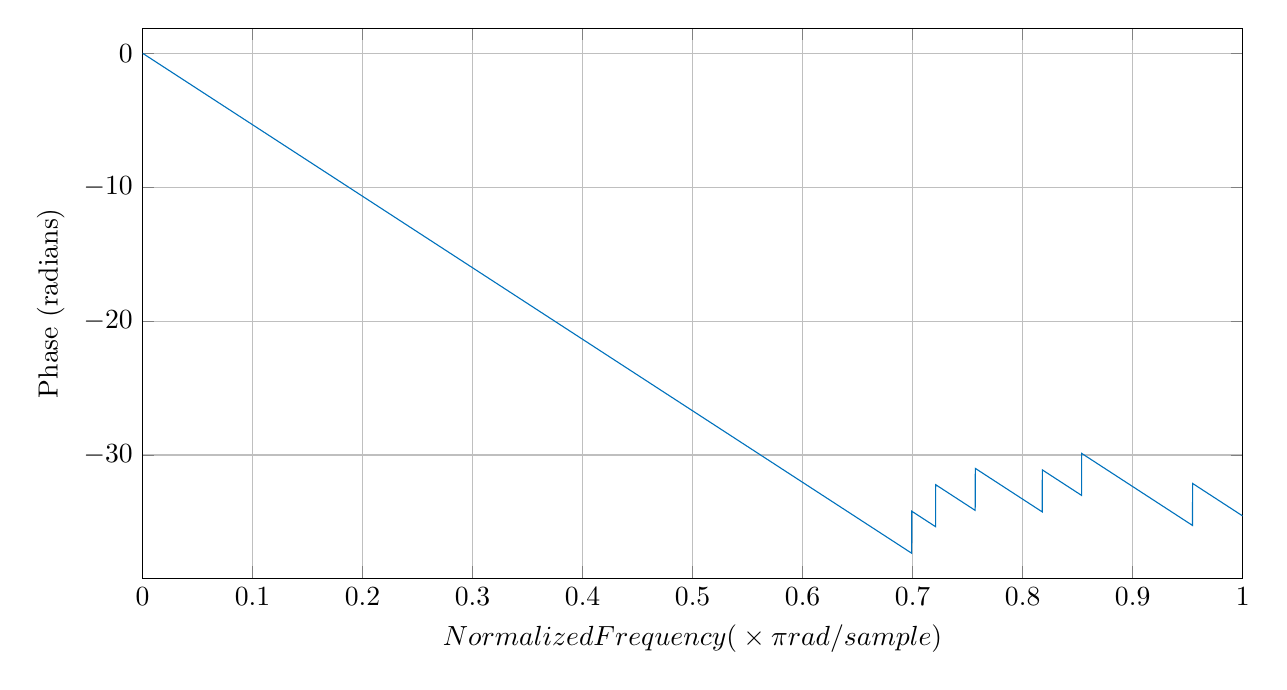
\begin{tikzpicture}

\begin{axis}[%
width=5.5in,
height=2.75in,
at={(1.281in,0.441in)},
scale only axis,
xmin=0,
xmax=0.9998779296875,
xlabel={$\text{Normalized Frequency (}\times\pi\text{ rad/sample)}$},
xmajorgrids,
ymin=-39.2035443260547,
ymax=1.86683544409784,
ylabel={Phase (radians)},
ymajorgrids,
axis background/.style={fill=white},
]
\addplot [color=mycolor1,solid,forget plot]
  table[row sep=crcr]{%
0	0\\
0.0001220703125	-0.00651941834851398\\
0.000244140625	-0.0130388366970279\\
0.0003662109375	-0.0195582550455419\\
0.00048828125	-0.026077673394056\\
0.0006103515625	-0.0325970917425699\\
0.000732421875	-0.0391165100910838\\
0.0008544921875	-0.0456359284395978\\
0.0009765625	-0.0521553467881119\\
0.0010986328125	-0.0586747651366257\\
0.001220703125	-0.0651941834851398\\
0.0013427734375	-0.0717136018336537\\
0.00146484375	-0.0782330201821677\\
0.0015869140625	-0.0847524385306818\\
0.001708984375	-0.0912718568791957\\
0.0018310546875	-0.0977912752277095\\
0.001953125	-0.104310693576224\\
0.0020751953125	-0.110830111924738\\
0.002197265625	-0.117349530273252\\
0.0023193359375	-0.123868948621765\\
0.00244140625	-0.13038836697028\\
0.0025634765625	-0.136907785318794\\
0.002685546875	-0.143427203667307\\
0.0028076171875	-0.149946622015821\\
0.0029296875	-0.156466040364335\\
0.0030517578125	-0.162985458712849\\
0.003173828125	-0.169504877061363\\
0.0032958984375	-0.176024295409877\\
0.00341796875	-0.182543713758391\\
0.0035400390625	-0.189063132106905\\
0.003662109375	-0.195582550455419\\
0.0037841796875	-0.202101968803933\\
0.00390625	-0.208621387152447\\
0.0040283203125	-0.215140805500961\\
0.004150390625	-0.221660223849475\\
0.0042724609375	-0.228179642197989\\
0.00439453125	-0.234699060546503\\
0.0045166015625	-0.241218478895017\\
0.004638671875	-0.247737897243531\\
0.0047607421875	-0.254257315592045\\
0.0048828125	-0.260776733940559\\
0.0050048828125	-0.267296152289073\\
0.005126953125	-0.273815570637587\\
0.0052490234375	-0.280334988986101\\
0.00537109375	-0.286854407334615\\
0.0054931640625	-0.293373825683129\\
0.005615234375	-0.299893244031643\\
0.0057373046875	-0.306412662380157\\
0.005859375	-0.312932080728671\\
0.0059814453125	-0.319451499077185\\
0.006103515625	-0.325970917425699\\
0.0062255859375	-0.332490335774213\\
0.00634765625	-0.339009754122727\\
0.0064697265625	-0.345529172471241\\
0.006591796875	-0.352048590819755\\
0.0067138671875	-0.358568009168269\\
0.0068359375	-0.365087427516783\\
0.0069580078125	-0.371606845865297\\
0.007080078125	-0.378126264213811\\
0.0072021484375	-0.384645682562325\\
0.00732421875	-0.391165100910838\\
0.0074462890625	-0.397684519259353\\
0.007568359375	-0.404203937607866\\
0.0076904296875	-0.41072335595638\\
0.0078125	-0.417242774304894\\
0.0079345703125	-0.423762192653408\\
0.008056640625	-0.430281611001922\\
0.0081787109375	-0.436801029350436\\
0.00830078125	-0.44332044769895\\
0.0084228515625	-0.449839866047464\\
0.008544921875	-0.456359284395978\\
0.0086669921875	-0.462878702744492\\
0.0087890625	-0.469398121093006\\
0.0089111328125	-0.47591753944152\\
0.009033203125	-0.482436957790034\\
0.0091552734375	-0.488956376138548\\
0.00927734375	-0.495475794487062\\
0.0093994140625	-0.501995212835576\\
0.009521484375	-0.50851463118409\\
0.0096435546875	-0.515034049532604\\
0.009765625	-0.521553467881118\\
0.0098876953125	-0.528072886229632\\
0.010009765625	-0.534592304578146\\
0.0101318359375	-0.54111172292666\\
0.01025390625	-0.547631141275174\\
0.0103759765625	-0.554150559623688\\
0.010498046875	-0.560669977972202\\
0.0106201171875	-0.567189396320716\\
0.0107421875	-0.57370881466923\\
0.0108642578125	-0.580228233017744\\
0.010986328125	-0.586747651366258\\
0.0111083984375	-0.593267069714772\\
0.01123046875	-0.599786488063286\\
0.0113525390625	-0.6063059064118\\
0.011474609375	-0.612825324760314\\
0.0115966796875	-0.619344743108828\\
0.01171875	-0.625864161457341\\
0.0118408203125	-0.632383579805855\\
0.011962890625	-0.638902998154369\\
0.0120849609375	-0.645422416502883\\
0.01220703125	-0.651941834851398\\
0.0123291015625	-0.658461253199912\\
0.012451171875	-0.664980671548425\\
0.0125732421875	-0.671500089896939\\
0.0126953125	-0.678019508245453\\
0.0128173828125	-0.684538926593967\\
0.012939453125	-0.691058344942481\\
0.0130615234375	-0.697577763290995\\
0.01318359375	-0.704097181639509\\
0.0133056640625	-0.710616599988023\\
0.013427734375	-0.717136018336537\\
0.0135498046875	-0.723655436685051\\
0.013671875	-0.730174855033565\\
0.0137939453125	-0.736694273382079\\
0.013916015625	-0.743213691730593\\
0.0140380859375	-0.749733110079107\\
0.01416015625	-0.756252528427621\\
0.0142822265625	-0.762771946776135\\
0.014404296875	-0.769291365124649\\
0.0145263671875	-0.775810783473163\\
0.0146484375	-0.782330201821677\\
0.0147705078125	-0.788849620170191\\
0.014892578125	-0.795369038518705\\
0.0150146484375	-0.801888456867219\\
0.01513671875	-0.808407875215733\\
0.0152587890625	-0.814927293564247\\
0.015380859375	-0.821446711912761\\
0.0155029296875	-0.827966130261275\\
0.015625	-0.834485548609789\\
0.0157470703125	-0.841004966958303\\
0.015869140625	-0.847524385306817\\
0.0159912109375	-0.854043803655331\\
0.01611328125	-0.860563222003845\\
0.0162353515625	-0.867082640352359\\
0.016357421875	-0.873602058700873\\
0.0164794921875	-0.880121477049387\\
0.0166015625	-0.886640895397901\\
0.0167236328125	-0.893160313746415\\
0.016845703125	-0.899679732094929\\
0.0169677734375	-0.906199150443443\\
0.01708984375	-0.912718568791957\\
0.0172119140625	-0.91923798714047\\
0.017333984375	-0.925757405488985\\
0.0174560546875	-0.932276823837498\\
0.017578125	-0.938796242186013\\
0.0177001953125	-0.945315660534526\\
0.017822265625	-0.95183507888304\\
0.0179443359375	-0.958354497231554\\
0.01806640625	-0.964873915580068\\
0.0181884765625	-0.971393333928582\\
0.018310546875	-0.977912752277096\\
0.0184326171875	-0.98443217062561\\
0.0185546875	-0.990951588974124\\
0.0186767578125	-0.997471007322638\\
0.018798828125	-1.00399042567115\\
0.0189208984375	-1.01050984401967\\
0.01904296875	-1.01702926236818\\
0.0191650390625	-1.02354868071669\\
0.019287109375	-1.03006809906521\\
0.0194091796875	-1.03658751741372\\
0.01953125	-1.04310693576224\\
0.0196533203125	-1.04962635411075\\
0.019775390625	-1.05614577245926\\
0.0198974609375	-1.06266519080778\\
0.02001953125	-1.06918460915629\\
0.0201416015625	-1.07570402750481\\
0.020263671875	-1.08222344585332\\
0.0203857421875	-1.08874286420183\\
0.0205078125	-1.09526228255035\\
0.0206298828125	-1.10178170089886\\
0.020751953125	-1.10830111924738\\
0.0208740234375	-1.11482053759589\\
0.02099609375	-1.1213399559444\\
0.0211181640625	-1.12785937429292\\
0.021240234375	-1.13437879264143\\
0.0213623046875	-1.14089821098995\\
0.021484375	-1.14741762933846\\
0.0216064453125	-1.15393704768697\\
0.021728515625	-1.16045646603549\\
0.0218505859375	-1.166975884384\\
0.02197265625	-1.17349530273252\\
0.0220947265625	-1.18001472108103\\
0.022216796875	-1.18653413942954\\
0.0223388671875	-1.19305355777806\\
0.0224609375	-1.19957297612657\\
0.0225830078125	-1.20609239447509\\
0.022705078125	-1.2126118128236\\
0.0228271484375	-1.21913123117211\\
0.02294921875	-1.22565064952063\\
0.0230712890625	-1.23217006786914\\
0.023193359375	-1.23868948621766\\
0.0233154296875	-1.24520890456617\\
0.0234375	-1.25172832291468\\
0.0235595703125	-1.2582477412632\\
0.023681640625	-1.26476715961171\\
0.0238037109375	-1.27128657796023\\
0.02392578125	-1.27780599630874\\
0.0240478515625	-1.28432541465725\\
0.024169921875	-1.29084483300577\\
0.0242919921875	-1.29736425135428\\
0.0244140625	-1.30388366970279\\
0.0245361328125	-1.31040308805131\\
0.024658203125	-1.31692250639982\\
0.0247802734375	-1.32344192474834\\
0.02490234375	-1.32996134309685\\
0.0250244140625	-1.33648076144536\\
0.025146484375	-1.34300017979388\\
0.0252685546875	-1.34951959814239\\
0.025390625	-1.35603901649091\\
0.0255126953125	-1.36255843483942\\
0.025634765625	-1.36907785318793\\
0.0257568359375	-1.37559727153645\\
0.02587890625	-1.38211668988496\\
0.0260009765625	-1.38863610823348\\
0.026123046875	-1.39515552658199\\
0.0262451171875	-1.4016749449305\\
0.0263671875	-1.40819436327902\\
0.0264892578125	-1.41471378162753\\
0.026611328125	-1.42123319997605\\
0.0267333984375	-1.42775261832456\\
0.02685546875	-1.43427203667307\\
0.0269775390625	-1.44079145502159\\
0.027099609375	-1.4473108733701\\
0.0272216796875	-1.45383029171862\\
0.02734375	-1.46034971006713\\
0.0274658203125	-1.46686912841564\\
0.027587890625	-1.47338854676416\\
0.0277099609375	-1.47990796511267\\
0.02783203125	-1.48642738346119\\
0.0279541015625	-1.4929468018097\\
0.028076171875	-1.49946622015821\\
0.0281982421875	-1.50598563850673\\
0.0283203125	-1.51250505685524\\
0.0284423828125	-1.51902447520376\\
0.028564453125	-1.52554389355227\\
0.0286865234375	-1.53206331190078\\
0.02880859375	-1.5385827302493\\
0.0289306640625	-1.54510214859781\\
0.029052734375	-1.55162156694633\\
0.0291748046875	-1.55814098529484\\
0.029296875	-1.56466040364335\\
0.0294189453125	-1.57117982199187\\
0.029541015625	-1.57769924034038\\
0.0296630859375	-1.5842186586889\\
0.02978515625	-1.59073807703741\\
0.0299072265625	-1.59725749538592\\
0.030029296875	-1.60377691373444\\
0.0301513671875	-1.61029633208295\\
0.0302734375	-1.61681575043147\\
0.0303955078125	-1.62333516877998\\
0.030517578125	-1.62985458712849\\
0.0306396484375	-1.63637400547701\\
0.03076171875	-1.64289342382552\\
0.0308837890625	-1.64941284217404\\
0.031005859375	-1.65593226052255\\
0.0311279296875	-1.66245167887106\\
0.03125	-1.66897109721958\\
0.0313720703125	-1.67549051556809\\
0.031494140625	-1.68200993391661\\
0.0316162109375	-1.68852935226512\\
0.03173828125	-1.69504877061363\\
0.0318603515625	-1.70156818896215\\
0.031982421875	-1.70808760731066\\
0.0321044921875	-1.71460702565918\\
0.0322265625	-1.72112644400769\\
0.0323486328125	-1.7276458623562\\
0.032470703125	-1.73416528070472\\
0.0325927734375	-1.74068469905323\\
0.03271484375	-1.74720411740175\\
0.0328369140625	-1.75372353575026\\
0.032958984375	-1.76024295409877\\
0.0330810546875	-1.76676237244729\\
0.033203125	-1.7732817907958\\
0.0333251953125	-1.77980120914432\\
0.033447265625	-1.78632062749283\\
0.0335693359375	-1.79284004584134\\
0.03369140625	-1.79935946418986\\
0.0338134765625	-1.80587888253837\\
0.033935546875	-1.81239830088689\\
0.0340576171875	-1.8189177192354\\
0.0341796875	-1.82543713758391\\
0.0343017578125	-1.83195655593243\\
0.034423828125	-1.83847597428094\\
0.0345458984375	-1.84499539262946\\
0.03466796875	-1.85151481097797\\
0.0347900390625	-1.85803422932648\\
0.034912109375	-1.864553647675\\
0.0350341796875	-1.87107306602351\\
0.03515625	-1.87759248437202\\
0.0352783203125	-1.88411190272054\\
0.035400390625	-1.89063132106905\\
0.0355224609375	-1.89715073941757\\
0.03564453125	-1.90367015776608\\
0.0357666015625	-1.91018957611459\\
0.035888671875	-1.91670899446311\\
0.0360107421875	-1.92322841281162\\
0.0361328125	-1.92974783116014\\
0.0362548828125	-1.93626724950865\\
0.036376953125	-1.94278666785716\\
0.0364990234375	-1.94930608620568\\
0.03662109375	-1.95582550455419\\
0.0367431640625	-1.96234492290271\\
0.036865234375	-1.96886434125122\\
0.0369873046875	-1.97538375959973\\
0.037109375	-1.98190317794825\\
0.0372314453125	-1.98842259629676\\
0.037353515625	-1.99494201464528\\
0.0374755859375	-2.00146143299379\\
0.03759765625	-2.0079808513423\\
0.0377197265625	-2.01450026969082\\
0.037841796875	-2.02101968803933\\
0.0379638671875	-2.02753910638785\\
0.0380859375	-2.03405852473636\\
0.0382080078125	-2.04057794308487\\
0.038330078125	-2.04709736143339\\
0.0384521484375	-2.0536167797819\\
0.03857421875	-2.06013619813042\\
0.0386962890625	-2.06665561647893\\
0.038818359375	-2.07317503482744\\
0.0389404296875	-2.07969445317596\\
0.0390625	-2.08621387152447\\
0.0391845703125	-2.09273328987299\\
0.039306640625	-2.0992527082215\\
0.0394287109375	-2.10577212657001\\
0.03955078125	-2.11229154491853\\
0.0396728515625	-2.11881096326704\\
0.039794921875	-2.12533038161556\\
0.0399169921875	-2.13184979996407\\
0.0400390625	-2.13836921831258\\
0.0401611328125	-2.1448886366611\\
0.040283203125	-2.15140805500961\\
0.0404052734375	-2.15792747335813\\
0.04052734375	-2.16444689170664\\
0.0406494140625	-2.17096631005515\\
0.040771484375	-2.17748572840367\\
0.0408935546875	-2.18400514675218\\
0.041015625	-2.1905245651007\\
0.0411376953125	-2.19704398344921\\
0.041259765625	-2.20356340179772\\
0.0413818359375	-2.21008282014624\\
0.04150390625	-2.21660223849475\\
0.0416259765625	-2.22312165684327\\
0.041748046875	-2.22964107519178\\
0.0418701171875	-2.23616049354029\\
0.0419921875	-2.24267991188881\\
0.0421142578125	-2.24919933023732\\
0.042236328125	-2.25571874858584\\
0.0423583984375	-2.26223816693435\\
0.04248046875	-2.26875758528286\\
0.0426025390625	-2.27527700363138\\
0.042724609375	-2.28179642197989\\
0.0428466796875	-2.28831584032841\\
0.04296875	-2.29483525867692\\
0.0430908203125	-2.30135467702543\\
0.043212890625	-2.30787409537395\\
0.0433349609375	-2.31439351372246\\
0.04345703125	-2.32091293207097\\
0.0435791015625	-2.32743235041949\\
0.043701171875	-2.333951768768\\
0.0438232421875	-2.34047118711652\\
0.0439453125	-2.34699060546503\\
0.0440673828125	-2.35351002381354\\
0.044189453125	-2.36002944216206\\
0.0443115234375	-2.36654886051057\\
0.04443359375	-2.37306827885909\\
0.0445556640625	-2.3795876972076\\
0.044677734375	-2.38610711555611\\
0.0447998046875	-2.39262653390463\\
0.044921875	-2.39914595225314\\
0.0450439453125	-2.40566537060166\\
0.045166015625	-2.41218478895017\\
0.0452880859375	-2.41870420729868\\
0.04541015625	-2.4252236256472\\
0.0455322265625	-2.43174304399571\\
0.045654296875	-2.43826246234423\\
0.0457763671875	-2.44478188069274\\
0.0458984375	-2.45130129904125\\
0.0460205078125	-2.45782071738977\\
0.046142578125	-2.46434013573828\\
0.0462646484375	-2.4708595540868\\
0.04638671875	-2.47737897243531\\
0.0465087890625	-2.48389839078382\\
0.046630859375	-2.49041780913234\\
0.0467529296875	-2.49693722748085\\
0.046875	-2.50345664582937\\
0.0469970703125	-2.50997606417788\\
0.047119140625	-2.51649548252639\\
0.0472412109375	-2.52301490087491\\
0.04736328125	-2.52953431922342\\
0.0474853515625	-2.53605373757194\\
0.047607421875	-2.54257315592045\\
0.0477294921875	-2.54909257426896\\
0.0478515625	-2.55561199261748\\
0.0479736328125	-2.56213141096599\\
0.048095703125	-2.56865082931451\\
0.0482177734375	-2.57517024766302\\
0.04833984375	-2.58168966601153\\
0.0484619140625	-2.58820908436005\\
0.048583984375	-2.59472850270856\\
0.0487060546875	-2.60124792105708\\
0.048828125	-2.60776733940559\\
0.0489501953125	-2.6142867577541\\
0.049072265625	-2.62080617610262\\
0.0491943359375	-2.62732559445113\\
0.04931640625	-2.63384501279965\\
0.0494384765625	-2.64036443114816\\
0.049560546875	-2.64688384949667\\
0.0496826171875	-2.65340326784519\\
0.0498046875	-2.6599226861937\\
0.0499267578125	-2.66644210454222\\
0.050048828125	-2.67296152289073\\
0.0501708984375	-2.67948094123924\\
0.05029296875	-2.68600035958776\\
0.0504150390625	-2.69251977793627\\
0.050537109375	-2.69903919628479\\
0.0506591796875	-2.7055586146333\\
0.05078125	-2.71207803298181\\
0.0509033203125	-2.71859745133033\\
0.051025390625	-2.72511686967884\\
0.0511474609375	-2.73163628802736\\
0.05126953125	-2.73815570637587\\
0.0513916015625	-2.74467512472438\\
0.051513671875	-2.7511945430729\\
0.0516357421875	-2.75771396142141\\
0.0517578125	-2.76423337976993\\
0.0518798828125	-2.77075279811844\\
0.052001953125	-2.77727221646695\\
0.0521240234375	-2.78379163481547\\
0.05224609375	-2.79031105316398\\
0.0523681640625	-2.7968304715125\\
0.052490234375	-2.80334988986101\\
0.0526123046875	-2.80986930820952\\
0.052734375	-2.81638872655804\\
0.0528564453125	-2.82290814490655\\
0.052978515625	-2.82942756325507\\
0.0531005859375	-2.83594698160358\\
0.05322265625	-2.84246639995209\\
0.0533447265625	-2.84898581830061\\
0.053466796875	-2.85550523664912\\
0.0535888671875	-2.86202465499764\\
0.0537109375	-2.86854407334615\\
0.0538330078125	-2.87506349169466\\
0.053955078125	-2.88158291004318\\
0.0540771484375	-2.88810232839169\\
0.05419921875	-2.89462174674021\\
0.0543212890625	-2.90114116508872\\
0.054443359375	-2.90766058343723\\
0.0545654296875	-2.91418000178575\\
0.0546875	-2.92069942013426\\
0.0548095703125	-2.92721883848278\\
0.054931640625	-2.93373825683129\\
0.0550537109375	-2.9402576751798\\
0.05517578125	-2.94677709352832\\
0.0552978515625	-2.95329651187683\\
0.055419921875	-2.95981593022534\\
0.0555419921875	-2.96633534857386\\
0.0556640625	-2.97285476692237\\
0.0557861328125	-2.97937418527089\\
0.055908203125	-2.9858936036194\\
0.0560302734375	-2.99241302196791\\
0.05615234375	-2.99893244031643\\
0.0562744140625	-3.00545185866494\\
0.056396484375	-3.01197127701346\\
0.0565185546875	-3.01849069536197\\
0.056640625	-3.02501011371048\\
0.0567626953125	-3.031529532059\\
0.056884765625	-3.03804895040751\\
0.0570068359375	-3.04456836875603\\
0.05712890625	-3.05108778710454\\
0.0572509765625	-3.05760720545305\\
0.057373046875	-3.06412662380157\\
0.0574951171875	-3.07064604215008\\
0.0576171875	-3.0771654604986\\
0.0577392578125	-3.08368487884711\\
0.057861328125	-3.09020429719562\\
0.0579833984375	-3.09672371554414\\
0.05810546875	-3.10324313389265\\
0.0582275390625	-3.10976255224117\\
0.058349609375	-3.11628197058968\\
0.0584716796875	-3.12280138893819\\
0.05859375	-3.12932080728671\\
0.0587158203125	-3.13584022563522\\
0.058837890625	-3.14235964398374\\
0.0589599609375	-3.14887906233225\\
0.05908203125	-3.15539848068076\\
0.0592041015625	-3.16191789902928\\
0.059326171875	-3.16843731737779\\
0.0594482421875	-3.17495673572631\\
0.0595703125	-3.18147615407482\\
0.0596923828125	-3.18799557242333\\
0.059814453125	-3.19451499077185\\
0.0599365234375	-3.20103440912036\\
0.06005859375	-3.20755382746888\\
0.0601806640625	-3.21407324581739\\
0.060302734375	-3.2205926641659\\
0.0604248046875	-3.22711208251442\\
0.060546875	-3.23363150086293\\
0.0606689453125	-3.24015091921145\\
0.060791015625	-3.24667033755996\\
0.0609130859375	-3.25318975590847\\
0.06103515625	-3.25970917425699\\
0.0611572265625	-3.2662285926055\\
0.061279296875	-3.27274801095402\\
0.0614013671875	-3.27926742930253\\
0.0615234375	-3.28578684765104\\
0.0616455078125	-3.29230626599956\\
0.061767578125	-3.29882568434807\\
0.0618896484375	-3.30534510269659\\
0.06201171875	-3.3118645210451\\
0.0621337890625	-3.31838393939361\\
0.062255859375	-3.32490335774213\\
0.0623779296875	-3.33142277609064\\
0.0625	-3.33794219443916\\
0.0626220703125	-3.34446161278767\\
0.062744140625	-3.35098103113618\\
0.0628662109375	-3.3575004494847\\
0.06298828125	-3.36401986783321\\
0.0631103515625	-3.37053928618172\\
0.063232421875	-3.37705870453024\\
0.0633544921875	-3.38357812287875\\
0.0634765625	-3.39009754122727\\
0.0635986328125	-3.39661695957578\\
0.063720703125	-3.40313637792429\\
0.0638427734375	-3.40965579627281\\
0.06396484375	-3.41617521462132\\
0.0640869140625	-3.42269463296984\\
0.064208984375	-3.42921405131835\\
0.0643310546875	-3.43573346966686\\
0.064453125	-3.44225288801538\\
0.0645751953125	-3.44877230636389\\
0.064697265625	-3.45529172471241\\
0.0648193359375	-3.46181114306092\\
0.06494140625	-3.46833056140943\\
0.0650634765625	-3.47484997975795\\
0.065185546875	-3.48136939810646\\
0.0653076171875	-3.48788881645498\\
0.0654296875	-3.49440823480349\\
0.0655517578125	-3.500927653152\\
0.065673828125	-3.50744707150052\\
0.0657958984375	-3.51396648984903\\
0.06591796875	-3.52048590819755\\
0.0660400390625	-3.52700532654606\\
0.066162109375	-3.53352474489457\\
0.0662841796875	-3.54004416324309\\
0.06640625	-3.5465635815916\\
0.0665283203125	-3.55308299994012\\
0.066650390625	-3.55960241828863\\
0.0667724609375	-3.56612183663714\\
0.06689453125	-3.57264125498566\\
0.0670166015625	-3.57916067333417\\
0.067138671875	-3.58568009168269\\
0.0672607421875	-3.5921995100312\\
0.0673828125	-3.59871892837971\\
0.0675048828125	-3.60523834672823\\
0.067626953125	-3.61175776507674\\
0.0677490234375	-3.61827718342526\\
0.06787109375	-3.62479660177377\\
0.0679931640625	-3.63131602012228\\
0.068115234375	-3.6378354384708\\
0.0682373046875	-3.64435485681931\\
0.068359375	-3.65087427516783\\
0.0684814453125	-3.65739369351634\\
0.068603515625	-3.66391311186485\\
0.0687255859375	-3.67043253021337\\
0.06884765625	-3.67695194856188\\
0.0689697265625	-3.6834713669104\\
0.069091796875	-3.68999078525891\\
0.0692138671875	-3.69651020360742\\
0.0693359375	-3.70302962195594\\
0.0694580078125	-3.70954904030445\\
0.069580078125	-3.71606845865297\\
0.0697021484375	-3.72258787700148\\
0.06982421875	-3.72910729534999\\
0.0699462890625	-3.73562671369851\\
0.070068359375	-3.74214613204702\\
0.0701904296875	-3.74866555039554\\
0.0703125	-3.75518496874405\\
0.0704345703125	-3.76170438709256\\
0.070556640625	-3.76822380544108\\
0.0706787109375	-3.77474322378959\\
0.07080078125	-3.78126264213811\\
0.0709228515625	-3.78778206048662\\
0.071044921875	-3.79430147883513\\
0.0711669921875	-3.80082089718365\\
0.0712890625	-3.80734031553216\\
0.0714111328125	-3.81385973388068\\
0.071533203125	-3.82037915222919\\
0.0716552734375	-3.8268985705777\\
0.07177734375	-3.83341798892622\\
0.0718994140625	-3.83993740727473\\
0.072021484375	-3.84645682562325\\
0.0721435546875	-3.85297624397176\\
0.072265625	-3.85949566232027\\
0.0723876953125	-3.86601508066879\\
0.072509765625	-3.8725344990173\\
0.0726318359375	-3.87905391736582\\
0.07275390625	-3.88557333571433\\
0.0728759765625	-3.89209275406284\\
0.072998046875	-3.89861217241136\\
0.0731201171875	-3.90513159075987\\
0.0732421875	-3.91165100910839\\
0.0733642578125	-3.9181704274569\\
0.073486328125	-3.92468984580541\\
0.0736083984375	-3.93120926415393\\
0.07373046875	-3.93772868250244\\
0.0738525390625	-3.94424810085096\\
0.073974609375	-3.95076751919947\\
0.0740966796875	-3.95728693754798\\
0.07421875	-3.9638063558965\\
0.0743408203125	-3.97032577424501\\
0.074462890625	-3.97684519259352\\
0.0745849609375	-3.98336461094204\\
0.07470703125	-3.98988402929055\\
0.0748291015625	-3.99640344763907\\
0.074951171875	-4.00292286598758\\
0.0750732421875	-4.00944228433609\\
0.0751953125	-4.01596170268461\\
0.0753173828125	-4.02248112103312\\
0.075439453125	-4.02900053938164\\
0.0755615234375	-4.03551995773015\\
0.07568359375	-4.04203937607866\\
0.0758056640625	-4.04855879442718\\
0.075927734375	-4.05507821277569\\
0.0760498046875	-4.06159763112421\\
0.076171875	-4.06811704947272\\
0.0762939453125	-4.07463646782123\\
0.076416015625	-4.08115588616975\\
0.0765380859375	-4.08767530451826\\
0.07666015625	-4.09419472286678\\
0.0767822265625	-4.10071414121529\\
0.076904296875	-4.1072335595638\\
0.0770263671875	-4.11375297791232\\
0.0771484375	-4.12027239626083\\
0.0772705078125	-4.12679181460935\\
0.077392578125	-4.13331123295786\\
0.0775146484375	-4.13983065130637\\
0.07763671875	-4.14635006965489\\
0.0777587890625	-4.1528694880034\\
0.077880859375	-4.15938890635192\\
0.0780029296875	-4.16590832470043\\
0.078125	-4.17242774304894\\
0.0782470703125	-4.17894716139746\\
0.078369140625	-4.18546657974597\\
0.0784912109375	-4.19198599809449\\
0.07861328125	-4.198505416443\\
0.0787353515625	-4.20502483479151\\
0.078857421875	-4.21154425314003\\
0.0789794921875	-4.21806367148854\\
0.0791015625	-4.22458308983706\\
0.0792236328125	-4.23110250818557\\
0.079345703125	-4.23762192653408\\
0.0794677734375	-4.2441413448826\\
0.07958984375	-4.25066076323111\\
0.0797119140625	-4.25718018157963\\
0.079833984375	-4.26369959992814\\
0.0799560546875	-4.27021901827665\\
0.080078125	-4.27673843662517\\
0.0802001953125	-4.28325785497368\\
0.080322265625	-4.2897772733222\\
0.0804443359375	-4.29629669167071\\
0.08056640625	-4.30281611001922\\
0.0806884765625	-4.30933552836774\\
0.080810546875	-4.31585494671625\\
0.0809326171875	-4.32237436506477\\
0.0810546875	-4.32889378341328\\
0.0811767578125	-4.33541320176179\\
0.081298828125	-4.34193262011031\\
0.0814208984375	-4.34845203845882\\
0.08154296875	-4.35497145680734\\
0.0816650390625	-4.36149087515585\\
0.081787109375	-4.36801029350436\\
0.0819091796875	-4.37452971185288\\
0.08203125	-4.38104913020139\\
0.0821533203125	-4.38756854854991\\
0.082275390625	-4.39408796689842\\
0.0823974609375	-4.40060738524693\\
0.08251953125	-4.40712680359545\\
0.0826416015625	-4.41364622194396\\
0.082763671875	-4.42016564029247\\
0.0828857421875	-4.42668505864099\\
0.0830078125	-4.4332044769895\\
0.0831298828125	-4.43972389533802\\
0.083251953125	-4.44624331368653\\
0.0833740234375	-4.45276273203504\\
0.08349609375	-4.45928215038356\\
0.0836181640625	-4.46580156873207\\
0.083740234375	-4.47232098708059\\
0.0838623046875	-4.4788404054291\\
0.083984375	-4.48535982377761\\
0.0841064453125	-4.49187924212613\\
0.084228515625	-4.49839866047464\\
0.0843505859375	-4.50491807882316\\
0.08447265625	-4.51143749717167\\
0.0845947265625	-4.51795691552018\\
0.084716796875	-4.5244763338687\\
0.0848388671875	-4.53099575221721\\
0.0849609375	-4.53751517056573\\
0.0850830078125	-4.54403458891424\\
0.085205078125	-4.55055400726275\\
0.0853271484375	-4.55707342561127\\
0.08544921875	-4.56359284395978\\
0.0855712890625	-4.5701122623083\\
0.085693359375	-4.57663168065681\\
0.0858154296875	-4.58315109900532\\
0.0859375	-4.58967051735384\\
0.0860595703125	-4.59618993570235\\
0.086181640625	-4.60270935405087\\
0.0863037109375	-4.60922877239938\\
0.08642578125	-4.61574819074789\\
0.0865478515625	-4.62226760909641\\
0.086669921875	-4.62878702744492\\
0.0867919921875	-4.63530644579344\\
0.0869140625	-4.64182586414195\\
0.0870361328125	-4.64834528249046\\
0.087158203125	-4.65486470083898\\
0.0872802734375	-4.66138411918749\\
0.08740234375	-4.66790353753601\\
0.0875244140625	-4.67442295588452\\
0.087646484375	-4.68094237423303\\
0.0877685546875	-4.68746179258155\\
0.087890625	-4.69398121093006\\
0.0880126953125	-4.70050062927858\\
0.088134765625	-4.70702004762709\\
0.0882568359375	-4.7135394659756\\
0.08837890625	-4.72005888432412\\
0.0885009765625	-4.72657830267263\\
0.088623046875	-4.73309772102115\\
0.0887451171875	-4.73961713936966\\
0.0888671875	-4.74613655771817\\
0.0889892578125	-4.75265597606669\\
0.089111328125	-4.7591753944152\\
0.0892333984375	-4.76569481276372\\
0.08935546875	-4.77221423111223\\
0.0894775390625	-4.77873364946074\\
0.089599609375	-4.78525306780926\\
0.0897216796875	-4.79177248615777\\
0.08984375	-4.79829190450629\\
0.0899658203125	-4.8048113228548\\
0.090087890625	-4.81133074120331\\
0.0902099609375	-4.81785015955183\\
0.09033203125	-4.82436957790034\\
0.0904541015625	-4.83088899624886\\
0.090576171875	-4.83740841459737\\
0.0906982421875	-4.84392783294588\\
0.0908203125	-4.8504472512944\\
0.0909423828125	-4.85696666964291\\
0.091064453125	-4.86348608799143\\
0.0911865234375	-4.87000550633994\\
0.09130859375	-4.87652492468845\\
0.0914306640625	-4.88304434303697\\
0.091552734375	-4.88956376138548\\
0.0916748046875	-4.896083179734\\
0.091796875	-4.90260259808251\\
0.0919189453125	-4.90912201643102\\
0.092041015625	-4.91564143477954\\
0.0921630859375	-4.92216085312805\\
0.09228515625	-4.92868027147656\\
0.0924072265625	-4.93519968982508\\
0.092529296875	-4.94171910817359\\
0.0926513671875	-4.94823852652211\\
0.0927734375	-4.95475794487062\\
0.0928955078125	-4.96127736321914\\
0.093017578125	-4.96779678156765\\
0.0931396484375	-4.97431619991616\\
0.09326171875	-4.98083561826468\\
0.0933837890625	-4.98735503661319\\
0.093505859375	-4.9938744549617\\
0.0936279296875	-5.00039387331022\\
0.09375	-5.00691329165873\\
0.0938720703125	-5.01343271000725\\
0.093994140625	-5.01995212835576\\
0.0941162109375	-5.02647154670427\\
0.09423828125	-5.03299096505279\\
0.0943603515625	-5.0395103834013\\
0.094482421875	-5.04602980174982\\
0.0946044921875	-5.05254922009833\\
0.0947265625	-5.05906863844684\\
0.0948486328125	-5.06558805679536\\
0.094970703125	-5.07210747514387\\
0.0950927734375	-5.07862689349239\\
0.09521484375	-5.0851463118409\\
0.0953369140625	-5.09166573018941\\
0.095458984375	-5.09818514853793\\
0.0955810546875	-5.10470456688644\\
0.095703125	-5.11122398523496\\
0.0958251953125	-5.11774340358347\\
0.095947265625	-5.12426282193198\\
0.0960693359375	-5.1307822402805\\
0.09619140625	-5.13730165862901\\
0.0963134765625	-5.14382107697753\\
0.096435546875	-5.15034049532604\\
0.0965576171875	-5.15685991367455\\
0.0966796875	-5.16337933202307\\
0.0968017578125	-5.16989875037158\\
0.096923828125	-5.1764181687201\\
0.0970458984375	-5.18293758706861\\
0.09716796875	-5.18945700541712\\
0.0972900390625	-5.19597642376564\\
0.097412109375	-5.20249584211415\\
0.0975341796875	-5.20901526046267\\
0.09765625	-5.21553467881118\\
0.0977783203125	-5.22205409715969\\
0.097900390625	-5.22857351550821\\
0.0980224609375	-5.23509293385672\\
0.09814453125	-5.24161235220524\\
0.0982666015625	-5.24813177055375\\
0.098388671875	-5.25465118890226\\
0.0985107421875	-5.26117060725078\\
0.0986328125	-5.26769002559929\\
0.0987548828125	-5.27420944394781\\
0.098876953125	-5.28072886229632\\
0.0989990234375	-5.28724828064483\\
0.09912109375	-5.29376769899335\\
0.0992431640625	-5.30028711734186\\
0.099365234375	-5.30680653569038\\
0.0994873046875	-5.31332595403889\\
0.099609375	-5.3198453723874\\
0.0997314453125	-5.32636479073592\\
0.099853515625	-5.33288420908443\\
0.0999755859375	-5.33940362743295\\
0.10009765625	-5.34592304578146\\
0.1002197265625	-5.35244246412997\\
0.100341796875	-5.35896188247849\\
0.1004638671875	-5.365481300827\\
0.1005859375	-5.37200071917552\\
0.1007080078125	-5.37852013752403\\
0.100830078125	-5.38503955587254\\
0.1009521484375	-5.39155897422106\\
0.10107421875	-5.39807839256957\\
0.1011962890625	-5.40459781091809\\
0.101318359375	-5.4111172292666\\
0.1014404296875	-5.41763664761511\\
0.1015625	-5.42415606596363\\
0.1016845703125	-5.43067548431214\\
0.101806640625	-5.43719490266066\\
0.1019287109375	-5.44371432100917\\
0.10205078125	-5.45023373935768\\
0.1021728515625	-5.4567531577062\\
0.102294921875	-5.46327257605471\\
0.1024169921875	-5.46979199440323\\
0.1025390625	-5.47631141275174\\
0.1026611328125	-5.48283083110025\\
0.102783203125	-5.48935024944877\\
0.1029052734375	-5.49586966779728\\
0.10302734375	-5.50238908614579\\
0.1031494140625	-5.50890850449431\\
0.103271484375	-5.51542792284282\\
0.1033935546875	-5.52194734119134\\
0.103515625	-5.52846675953985\\
0.1036376953125	-5.53498617788836\\
0.103759765625	-5.54150559623688\\
0.1038818359375	-5.54802501458539\\
0.10400390625	-5.55454443293391\\
0.1041259765625	-5.56106385128242\\
0.104248046875	-5.56758326963093\\
0.1043701171875	-5.57410268797945\\
0.1044921875	-5.58062210632796\\
0.1046142578125	-5.58714152467648\\
0.104736328125	-5.59366094302499\\
0.1048583984375	-5.6001803613735\\
0.10498046875	-5.60669977972202\\
0.1051025390625	-5.61321919807053\\
0.105224609375	-5.61973861641905\\
0.1053466796875	-5.62625803476756\\
0.10546875	-5.63277745311607\\
0.1055908203125	-5.63929687146459\\
0.105712890625	-5.6458162898131\\
0.1058349609375	-5.65233570816162\\
0.10595703125	-5.65885512651013\\
0.1060791015625	-5.66537454485864\\
0.106201171875	-5.67189396320716\\
0.1063232421875	-5.67841338155567\\
0.1064453125	-5.68493279990419\\
0.1065673828125	-5.6914522182527\\
0.106689453125	-5.69797163660121\\
0.1068115234375	-5.70449105494973\\
0.10693359375	-5.71101047329824\\
0.1070556640625	-5.71752989164676\\
0.107177734375	-5.72404930999527\\
0.1072998046875	-5.73056872834378\\
0.107421875	-5.7370881466923\\
0.1075439453125	-5.74360756504081\\
0.107666015625	-5.75012698338933\\
0.1077880859375	-5.75664640173784\\
0.10791015625	-5.76316582008635\\
0.1080322265625	-5.76968523843487\\
0.108154296875	-5.77620465678338\\
0.1082763671875	-5.7827240751319\\
0.1083984375	-5.78924349348041\\
0.1085205078125	-5.79576291182892\\
0.108642578125	-5.80228233017744\\
0.1087646484375	-5.80880174852595\\
0.10888671875	-5.81532116687447\\
0.1090087890625	-5.82184058522298\\
0.109130859375	-5.82836000357149\\
0.1092529296875	-5.83487942192001\\
0.109375	-5.84139884026852\\
0.1094970703125	-5.84791825861704\\
0.109619140625	-5.85443767696555\\
0.1097412109375	-5.86095709531406\\
0.10986328125	-5.86747651366258\\
0.1099853515625	-5.87399593201109\\
0.110107421875	-5.88051535035961\\
0.1102294921875	-5.88703476870812\\
0.1103515625	-5.89355418705663\\
0.1104736328125	-5.90007360540515\\
0.110595703125	-5.90659302375366\\
0.1107177734375	-5.91311244210218\\
0.11083984375	-5.91963186045069\\
0.1109619140625	-5.9261512787992\\
0.111083984375	-5.93267069714772\\
0.1112060546875	-5.93919011549623\\
0.111328125	-5.94570953384475\\
0.1114501953125	-5.95222895219326\\
0.111572265625	-5.95874837054177\\
0.1116943359375	-5.96526778889029\\
0.11181640625	-5.9717872072388\\
0.1119384765625	-5.97830662558732\\
0.112060546875	-5.98482604393583\\
0.1121826171875	-5.99134546228434\\
0.1123046875	-5.99786488063286\\
0.1124267578125	-6.00438429898137\\
0.112548828125	-6.01090371732989\\
0.1126708984375	-6.0174231356784\\
0.11279296875	-6.02394255402691\\
0.1129150390625	-6.03046197237543\\
0.113037109375	-6.03698139072394\\
0.1131591796875	-6.04350080907246\\
0.11328125	-6.05002022742097\\
0.1134033203125	-6.05653964576948\\
0.113525390625	-6.063059064118\\
0.1136474609375	-6.06957848246651\\
0.11376953125	-6.07609790081503\\
0.1138916015625	-6.08261731916354\\
0.114013671875	-6.08913673751205\\
0.1141357421875	-6.09565615586057\\
0.1142578125	-6.10217557420908\\
0.1143798828125	-6.10869499255759\\
0.114501953125	-6.11521441090611\\
0.1146240234375	-6.12173382925462\\
0.11474609375	-6.12825324760314\\
0.1148681640625	-6.13477266595165\\
0.114990234375	-6.14129208430017\\
0.1151123046875	-6.14781150264868\\
0.115234375	-6.15433092099719\\
0.1153564453125	-6.16085033934571\\
0.115478515625	-6.16736975769422\\
0.1156005859375	-6.17388917604273\\
0.11572265625	-6.18040859439125\\
0.1158447265625	-6.18692801273976\\
0.115966796875	-6.19344743108828\\
0.1160888671875	-6.19996684943679\\
0.1162109375	-6.2064862677853\\
0.1163330078125	-6.21300568613382\\
0.116455078125	-6.21952510448233\\
0.1165771484375	-6.22604452283085\\
0.11669921875	-6.23256394117936\\
0.1168212890625	-6.23908335952787\\
0.116943359375	-6.24560277787639\\
0.1170654296875	-6.2521221962249\\
0.1171875	-6.25864161457342\\
0.1173095703125	-6.26516103292193\\
0.117431640625	-6.27168045127044\\
0.1175537109375	-6.27819986961896\\
0.11767578125	-6.28471928796747\\
0.1177978515625	-6.29123870631599\\
0.117919921875	-6.2977581246645\\
0.1180419921875	-6.30427754301301\\
0.1181640625	-6.31079696136153\\
0.1182861328125	-6.31731637971004\\
0.118408203125	-6.32383579805856\\
0.1185302734375	-6.33035521640707\\
0.11865234375	-6.33687463475558\\
0.1187744140625	-6.3433940531041\\
0.118896484375	-6.34991347145261\\
0.1190185546875	-6.35643288980113\\
0.119140625	-6.36295230814964\\
0.1192626953125	-6.36947172649815\\
0.119384765625	-6.37599114484667\\
0.1195068359375	-6.38251056319518\\
0.11962890625	-6.3890299815437\\
0.1197509765625	-6.39554939989221\\
0.119873046875	-6.40206881824072\\
0.1199951171875	-6.40858823658924\\
0.1201171875	-6.41510765493775\\
0.1202392578125	-6.42162707328627\\
0.120361328125	-6.42814649163478\\
0.1204833984375	-6.43466590998329\\
0.12060546875	-6.44118532833181\\
0.1207275390625	-6.44770474668032\\
0.120849609375	-6.45422416502884\\
0.1209716796875	-6.46074358337735\\
0.12109375	-6.46726300172586\\
0.1212158203125	-6.47378242007438\\
0.121337890625	-6.48030183842289\\
0.1214599609375	-6.48682125677141\\
0.12158203125	-6.49334067511992\\
0.1217041015625	-6.49986009346843\\
0.121826171875	-6.50637951181695\\
0.1219482421875	-6.51289893016546\\
0.1220703125	-6.51941834851397\\
0.1221923828125	-6.52593776686249\\
0.122314453125	-6.532457185211\\
0.1224365234375	-6.53897660355952\\
0.12255859375	-6.54549602190803\\
0.1226806640625	-6.55201544025654\\
0.122802734375	-6.55853485860506\\
0.1229248046875	-6.56505427695357\\
0.123046875	-6.57157369530209\\
0.1231689453125	-6.5780931136506\\
0.123291015625	-6.58461253199911\\
0.1234130859375	-6.59113195034763\\
0.12353515625	-6.59765136869614\\
0.1236572265625	-6.60417078704466\\
0.123779296875	-6.61069020539317\\
0.1239013671875	-6.61720962374168\\
0.1240234375	-6.6237290420902\\
0.1241455078125	-6.63024846043871\\
0.124267578125	-6.63676787878723\\
0.1243896484375	-6.64328729713574\\
0.12451171875	-6.64980671548425\\
0.1246337890625	-6.65632613383277\\
0.124755859375	-6.66284555218128\\
0.1248779296875	-6.6693649705298\\
0.125	-6.67588438887831\\
0.1251220703125	-6.68240380722682\\
0.125244140625	-6.68892322557534\\
0.1253662109375	-6.69544264392385\\
0.12548828125	-6.70196206227237\\
0.1256103515625	-6.70848148062088\\
0.125732421875	-6.71500089896939\\
0.1258544921875	-6.72152031731791\\
0.1259765625	-6.72803973566642\\
0.1260986328125	-6.73455915401494\\
0.126220703125	-6.74107857236345\\
0.1263427734375	-6.74759799071196\\
0.12646484375	-6.75411740906048\\
0.1265869140625	-6.76063682740899\\
0.126708984375	-6.76715624575751\\
0.1268310546875	-6.77367566410602\\
0.126953125	-6.78019508245453\\
0.1270751953125	-6.78671450080305\\
0.127197265625	-6.79323391915156\\
0.1273193359375	-6.79975333750008\\
0.12744140625	-6.80627275584859\\
0.1275634765625	-6.8127921741971\\
0.127685546875	-6.81931159254562\\
0.1278076171875	-6.82583101089413\\
0.1279296875	-6.83235042924265\\
0.1280517578125	-6.83886984759116\\
0.128173828125	-6.84538926593967\\
0.1282958984375	-6.85190868428819\\
0.12841796875	-6.8584281026367\\
0.1285400390625	-6.86494752098522\\
0.128662109375	-6.87146693933373\\
0.1287841796875	-6.87798635768224\\
0.12890625	-6.88450577603076\\
0.1290283203125	-6.89102519437927\\
0.129150390625	-6.89754461272779\\
0.1292724609375	-6.9040640310763\\
0.12939453125	-6.91058344942481\\
0.1295166015625	-6.91710286777333\\
0.129638671875	-6.92362228612184\\
0.1297607421875	-6.93014170447036\\
0.1298828125	-6.93666112281887\\
0.1300048828125	-6.94318054116738\\
0.130126953125	-6.9496999595159\\
0.1302490234375	-6.95621937786441\\
0.13037109375	-6.96273879621293\\
0.1304931640625	-6.96925821456144\\
0.130615234375	-6.97577763290995\\
0.1307373046875	-6.98229705125847\\
0.130859375	-6.98881646960698\\
0.1309814453125	-6.99533588795549\\
0.131103515625	-7.00185530630401\\
0.1312255859375	-7.00837472465252\\
0.13134765625	-7.01489414300104\\
0.1314697265625	-7.02141356134955\\
0.131591796875	-7.02793297969806\\
0.1317138671875	-7.03445239804658\\
0.1318359375	-7.04097181639509\\
0.1319580078125	-7.04749123474361\\
0.132080078125	-7.05401065309212\\
0.1322021484375	-7.06053007144063\\
0.13232421875	-7.06704948978915\\
0.1324462890625	-7.07356890813766\\
0.132568359375	-7.08008832648618\\
0.1326904296875	-7.08660774483469\\
0.1328125	-7.0931271631832\\
0.1329345703125	-7.09964658153172\\
0.133056640625	-7.10616599988023\\
0.1331787109375	-7.11268541822875\\
0.13330078125	-7.11920483657726\\
0.1334228515625	-7.12572425492577\\
0.133544921875	-7.13224367327429\\
0.1336669921875	-7.1387630916228\\
0.1337890625	-7.14528250997132\\
0.1339111328125	-7.15180192831983\\
0.134033203125	-7.15832134666834\\
0.1341552734375	-7.16484076501686\\
0.13427734375	-7.17136018336537\\
0.1343994140625	-7.17787960171389\\
0.134521484375	-7.1843990200624\\
0.1346435546875	-7.19091843841091\\
0.134765625	-7.19743785675943\\
0.1348876953125	-7.20395727510794\\
0.135009765625	-7.21047669345646\\
0.1351318359375	-7.21699611180497\\
0.13525390625	-7.22351553015348\\
0.1353759765625	-7.230034948502\\
0.135498046875	-7.23655436685051\\
0.1356201171875	-7.24307378519903\\
0.1357421875	-7.24959320354754\\
0.1358642578125	-7.25611262189605\\
0.135986328125	-7.26263204024457\\
0.1361083984375	-7.26915145859308\\
0.13623046875	-7.2756708769416\\
0.1363525390625	-7.28219029529011\\
0.136474609375	-7.28870971363862\\
0.1365966796875	-7.29522913198714\\
0.13671875	-7.30174855033565\\
0.1368408203125	-7.30826796868417\\
0.136962890625	-7.31478738703268\\
0.1370849609375	-7.32130680538119\\
0.13720703125	-7.32782622372971\\
0.1373291015625	-7.33434564207822\\
0.137451171875	-7.34086506042674\\
0.1375732421875	-7.34738447877525\\
0.1376953125	-7.35390389712376\\
0.1378173828125	-7.36042331547228\\
0.137939453125	-7.36694273382079\\
0.1380615234375	-7.37346215216931\\
0.13818359375	-7.37998157051782\\
0.1383056640625	-7.38650098886633\\
0.138427734375	-7.39302040721485\\
0.1385498046875	-7.39953982556336\\
0.138671875	-7.40605924391188\\
0.1387939453125	-7.41257866226039\\
0.138916015625	-7.4190980806089\\
0.1390380859375	-7.42561749895742\\
0.13916015625	-7.43213691730593\\
0.1392822265625	-7.43865633565445\\
0.139404296875	-7.44517575400296\\
0.1395263671875	-7.45169517235147\\
0.1396484375	-7.45821459069999\\
0.1397705078125	-7.4647340090485\\
0.139892578125	-7.47125342739702\\
0.1400146484375	-7.47777284574553\\
0.14013671875	-7.48429226409404\\
0.1402587890625	-7.49081168244256\\
0.140380859375	-7.49733110079107\\
0.1405029296875	-7.50385051913959\\
0.140625	-7.5103699374881\\
0.1407470703125	-7.51688935583661\\
0.140869140625	-7.52340877418513\\
0.1409912109375	-7.52992819253364\\
0.14111328125	-7.53644761088216\\
0.1412353515625	-7.54296702923067\\
0.141357421875	-7.54948644757918\\
0.1414794921875	-7.5560058659277\\
0.1416015625	-7.56252528427621\\
0.1417236328125	-7.56904470262473\\
0.141845703125	-7.57556412097324\\
0.1419677734375	-7.58208353932175\\
0.14208984375	-7.58860295767027\\
0.1422119140625	-7.59512237601878\\
0.142333984375	-7.6016417943673\\
0.1424560546875	-7.60816121271581\\
0.142578125	-7.61468063106432\\
0.1427001953125	-7.62120004941284\\
0.142822265625	-7.62771946776135\\
0.1429443359375	-7.63423888610986\\
0.14306640625	-7.64075830445838\\
0.1431884765625	-7.64727772280689\\
0.143310546875	-7.65379714115541\\
0.1434326171875	-7.66031655950392\\
0.1435546875	-7.66683597785243\\
0.1436767578125	-7.67335539620095\\
0.143798828125	-7.67987481454946\\
0.1439208984375	-7.68639423289798\\
0.14404296875	-7.69291365124649\\
0.1441650390625	-7.699433069595\\
0.144287109375	-7.70595248794352\\
0.1444091796875	-7.71247190629203\\
0.14453125	-7.71899132464055\\
0.1446533203125	-7.72551074298906\\
0.144775390625	-7.73203016133757\\
0.1448974609375	-7.73854957968609\\
0.14501953125	-7.7450689980346\\
0.1451416015625	-7.75158841638312\\
0.145263671875	-7.75810783473163\\
0.1453857421875	-7.76462725308014\\
0.1455078125	-7.77114667142866\\
0.1456298828125	-7.77766608977717\\
0.145751953125	-7.78418550812569\\
0.1458740234375	-7.7907049264742\\
0.14599609375	-7.79722434482271\\
0.1461181640625	-7.80374376317123\\
0.146240234375	-7.81026318151974\\
0.1463623046875	-7.81678259986826\\
0.146484375	-7.82330201821677\\
0.1466064453125	-7.82982143656528\\
0.146728515625	-7.8363408549138\\
0.1468505859375	-7.84286027326231\\
0.14697265625	-7.84937969161083\\
0.1470947265625	-7.85589910995934\\
0.147216796875	-7.86241852830785\\
0.1473388671875	-7.86893794665637\\
0.1474609375	-7.87545736500488\\
0.1475830078125	-7.8819767833534\\
0.147705078125	-7.88849620170191\\
0.1478271484375	-7.89501562005042\\
0.14794921875	-7.90153503839894\\
0.1480712890625	-7.90805445674745\\
0.148193359375	-7.91457387509597\\
0.1483154296875	-7.92109329344448\\
0.1484375	-7.92761271179299\\
0.1485595703125	-7.93413213014151\\
0.148681640625	-7.94065154849002\\
0.1488037109375	-7.94717096683854\\
0.14892578125	-7.95369038518705\\
0.1490478515625	-7.96020980353556\\
0.149169921875	-7.96672922188408\\
0.1492919921875	-7.97324864023259\\
0.1494140625	-7.97976805858111\\
0.1495361328125	-7.98628747692962\\
0.149658203125	-7.99280689527813\\
0.1497802734375	-7.99932631362665\\
0.14990234375	-8.00584573197516\\
0.1500244140625	-8.01236515032368\\
0.150146484375	-8.01888456867219\\
0.1502685546875	-8.0254039870207\\
0.150390625	-8.03192340536922\\
0.1505126953125	-8.03844282371773\\
0.150634765625	-8.04496224206625\\
0.1507568359375	-8.05148166041476\\
0.15087890625	-8.05800107876327\\
0.1510009765625	-8.06452049711179\\
0.151123046875	-8.0710399154603\\
0.1512451171875	-8.07755933380882\\
0.1513671875	-8.08407875215733\\
0.1514892578125	-8.09059817050584\\
0.151611328125	-8.09711758885436\\
0.1517333984375	-8.10363700720287\\
0.15185546875	-8.11015642555138\\
0.1519775390625	-8.1166758438999\\
0.152099609375	-8.12319526224841\\
0.1522216796875	-8.12971468059693\\
0.15234375	-8.13623409894544\\
0.1524658203125	-8.14275351729395\\
0.152587890625	-8.14927293564247\\
0.1527099609375	-8.15579235399098\\
0.15283203125	-8.1623117723395\\
0.1529541015625	-8.16883119068801\\
0.153076171875	-8.17535060903652\\
0.1531982421875	-8.18187002738504\\
0.1533203125	-8.18838944573355\\
0.1534423828125	-8.19490886408207\\
0.153564453125	-8.20142828243058\\
0.1536865234375	-8.20794770077909\\
0.15380859375	-8.21446711912761\\
0.1539306640625	-8.22098653747612\\
0.154052734375	-8.22750595582464\\
0.1541748046875	-8.23402537417315\\
0.154296875	-8.24054479252166\\
0.1544189453125	-8.24706421087018\\
0.154541015625	-8.25358362921869\\
0.1546630859375	-8.26010304756721\\
0.15478515625	-8.26662246591572\\
0.1549072265625	-8.27314188426423\\
0.155029296875	-8.27966130261275\\
0.1551513671875	-8.28618072096126\\
0.1552734375	-8.29270013930978\\
0.1553955078125	-8.29921955765829\\
0.155517578125	-8.3057389760068\\
0.1556396484375	-8.31225839435532\\
0.15576171875	-8.31877781270383\\
0.1558837890625	-8.32529723105235\\
0.156005859375	-8.33181664940086\\
0.1561279296875	-8.33833606774937\\
0.15625	-8.34485548609789\\
0.1563720703125	-8.3513749044464\\
0.156494140625	-8.35789432279492\\
0.1566162109375	-8.36441374114343\\
0.15673828125	-8.37093315949194\\
0.1568603515625	-8.37745257784046\\
0.156982421875	-8.38397199618897\\
0.1571044921875	-8.39049141453749\\
0.1572265625	-8.397010832886\\
0.1573486328125	-8.40353025123451\\
0.157470703125	-8.41004966958303\\
0.1575927734375	-8.41656908793154\\
0.15771484375	-8.42308850628006\\
0.1578369140625	-8.42960792462857\\
0.157958984375	-8.43612734297708\\
0.1580810546875	-8.4426467613256\\
0.158203125	-8.44916617967411\\
0.1583251953125	-8.45568559802263\\
0.158447265625	-8.46220501637114\\
0.1585693359375	-8.46872443471965\\
0.15869140625	-8.47524385306817\\
0.1588134765625	-8.48176327141668\\
0.158935546875	-8.4882826897652\\
0.1590576171875	-8.49480210811371\\
0.1591796875	-8.50132152646222\\
0.1593017578125	-8.50784094481074\\
0.159423828125	-8.51436036315925\\
0.1595458984375	-8.52087978150777\\
0.15966796875	-8.52739919985628\\
0.1597900390625	-8.53391861820479\\
0.159912109375	-8.54043803655331\\
0.1600341796875	-8.54695745490182\\
0.16015625	-8.55347687325034\\
0.1602783203125	-8.55999629159885\\
0.160400390625	-8.56651570994736\\
0.1605224609375	-8.57303512829588\\
0.16064453125	-8.57955454664439\\
0.1607666015625	-8.58607396499291\\
0.160888671875	-8.59259338334142\\
0.1610107421875	-8.59911280168993\\
0.1611328125	-8.60563222003845\\
0.1612548828125	-8.61215163838696\\
0.161376953125	-8.61867105673548\\
0.1614990234375	-8.62519047508399\\
0.16162109375	-8.6317098934325\\
0.1617431640625	-8.63822931178102\\
0.161865234375	-8.64474873012953\\
0.1619873046875	-8.65126814847805\\
0.162109375	-8.65778756682656\\
0.1622314453125	-8.66430698517507\\
0.162353515625	-8.67082640352359\\
0.1624755859375	-8.6773458218721\\
0.16259765625	-8.68386524022062\\
0.1627197265625	-8.69038465856913\\
0.162841796875	-8.69690407691764\\
0.1629638671875	-8.70342349526616\\
0.1630859375	-8.70994291361467\\
0.1632080078125	-8.71646233196319\\
0.163330078125	-8.7229817503117\\
0.1634521484375	-8.72950116866021\\
0.16357421875	-8.73602058700873\\
0.1636962890625	-8.74254000535724\\
0.163818359375	-8.74905942370576\\
0.1639404296875	-8.75557884205427\\
0.1640625	-8.76209826040278\\
0.1641845703125	-8.7686176787513\\
0.164306640625	-8.77513709709981\\
0.1644287109375	-8.78165651544832\\
0.16455078125	-8.78817593379684\\
0.1646728515625	-8.79469535214535\\
0.164794921875	-8.80121477049387\\
0.1649169921875	-8.80773418884238\\
0.1650390625	-8.81425360719089\\
0.1651611328125	-8.82077302553941\\
0.165283203125	-8.82729244388792\\
0.1654052734375	-8.83381186223644\\
0.16552734375	-8.84033128058495\\
0.1656494140625	-8.84685069893346\\
0.165771484375	-8.85337011728198\\
0.1658935546875	-8.85988953563049\\
0.166015625	-8.86640895397901\\
0.1661376953125	-8.87292837232752\\
0.166259765625	-8.87944779067603\\
0.1663818359375	-8.88596720902455\\
0.16650390625	-8.89248662737306\\
0.1666259765625	-8.89900604572158\\
0.166748046875	-8.90552546407009\\
0.1668701171875	-8.9120448824186\\
0.1669921875	-8.91856430076712\\
0.1671142578125	-8.92508371911563\\
0.167236328125	-8.93160313746415\\
0.1673583984375	-8.93812255581266\\
0.16748046875	-8.94464197416117\\
0.1676025390625	-8.95116139250969\\
0.167724609375	-8.9576808108582\\
0.1678466796875	-8.96420022920672\\
0.16796875	-8.97071964755523\\
0.1680908203125	-8.97723906590374\\
0.168212890625	-8.98375848425226\\
0.1683349609375	-8.99027790260077\\
0.16845703125	-8.99679732094929\\
0.1685791015625	-9.0033167392978\\
0.168701171875	-9.00983615764631\\
0.1688232421875	-9.01635557599483\\
0.1689453125	-9.02287499434334\\
0.1690673828125	-9.02939441269186\\
0.169189453125	-9.03591383104037\\
0.1693115234375	-9.04243324938888\\
0.16943359375	-9.0489526677374\\
0.1695556640625	-9.05547208608591\\
0.169677734375	-9.06199150443443\\
0.1697998046875	-9.06851092278294\\
0.169921875	-9.07503034113145\\
0.1700439453125	-9.08154975947997\\
0.170166015625	-9.08806917782848\\
0.1702880859375	-9.094588596177\\
0.17041015625	-9.10110801452551\\
0.1705322265625	-9.10762743287402\\
0.170654296875	-9.11414685122254\\
0.1707763671875	-9.12066626957105\\
0.1708984375	-9.12718568791957\\
0.1710205078125	-9.13370510626808\\
0.171142578125	-9.14022452461659\\
0.1712646484375	-9.14674394296511\\
0.17138671875	-9.15326336131362\\
0.1715087890625	-9.15978277966214\\
0.171630859375	-9.16630219801065\\
0.1717529296875	-9.17282161635916\\
0.171875	-9.17934103470768\\
0.1719970703125	-9.18586045305619\\
0.172119140625	-9.1923798714047\\
0.1722412109375	-9.19889928975322\\
0.17236328125	-9.20541870810173\\
0.1724853515625	-9.21193812645025\\
0.172607421875	-9.21845754479876\\
0.1727294921875	-9.22497696314727\\
0.1728515625	-9.23149638149579\\
0.1729736328125	-9.2380157998443\\
0.173095703125	-9.24453521819282\\
0.1732177734375	-9.25105463654133\\
0.17333984375	-9.25757405488984\\
0.1734619140625	-9.26409347323836\\
0.173583984375	-9.27061289158687\\
0.1737060546875	-9.27713230993539\\
0.173828125	-9.2836517282839\\
0.1739501953125	-9.29017114663241\\
0.174072265625	-9.29669056498093\\
0.1741943359375	-9.30320998332944\\
0.17431640625	-9.30972940167796\\
0.1744384765625	-9.31624882002647\\
0.174560546875	-9.32276823837498\\
0.1746826171875	-9.3292876567235\\
0.1748046875	-9.33580707507201\\
0.1749267578125	-9.34232649342053\\
0.175048828125	-9.34884591176904\\
0.1751708984375	-9.35536533011755\\
0.17529296875	-9.36188474846607\\
0.1754150390625	-9.36840416681458\\
0.175537109375	-9.3749235851631\\
0.1756591796875	-9.38144300351161\\
0.17578125	-9.38796242186012\\
0.1759033203125	-9.39448184020864\\
0.176025390625	-9.40100125855715\\
0.1761474609375	-9.40752067690567\\
0.17626953125	-9.41404009525418\\
0.1763916015625	-9.42055951360269\\
0.176513671875	-9.42707893195121\\
0.1766357421875	-9.43359835029972\\
0.1767578125	-9.44011776864824\\
0.1768798828125	-9.44663718699675\\
0.177001953125	-9.45315660534526\\
0.1771240234375	-9.45967602369378\\
0.17724609375	-9.46619544204229\\
0.1773681640625	-9.47271486039081\\
0.177490234375	-9.47923427873932\\
0.1776123046875	-9.48575369708783\\
0.177734375	-9.49227311543635\\
0.1778564453125	-9.49879253378486\\
0.177978515625	-9.50531195213338\\
0.1781005859375	-9.51183137048189\\
0.17822265625	-9.5183507888304\\
0.1783447265625	-9.52487020717892\\
0.178466796875	-9.53138962552743\\
0.1785888671875	-9.53790904387595\\
0.1787109375	-9.54442846222446\\
0.1788330078125	-9.55094788057297\\
0.178955078125	-9.55746729892149\\
0.1790771484375	-9.56398671727\\
0.17919921875	-9.57050613561852\\
0.1793212890625	-9.57702555396703\\
0.179443359375	-9.58354497231554\\
0.1795654296875	-9.59006439066406\\
0.1796875	-9.59658380901257\\
0.1798095703125	-9.60310322736109\\
0.179931640625	-9.6096226457096\\
0.1800537109375	-9.61614206405811\\
0.18017578125	-9.62266148240663\\
0.1802978515625	-9.62918090075514\\
0.180419921875	-9.63570031910366\\
0.1805419921875	-9.64221973745217\\
0.1806640625	-9.64873915580068\\
0.1807861328125	-9.6552585741492\\
0.180908203125	-9.66177799249771\\
0.1810302734375	-9.66829741084623\\
0.18115234375	-9.67481682919474\\
0.1812744140625	-9.68133624754325\\
0.181396484375	-9.68785566589177\\
0.1815185546875	-9.69437508424028\\
0.181640625	-9.7008945025888\\
0.1817626953125	-9.70741392093731\\
0.181884765625	-9.71393333928582\\
0.1820068359375	-9.72045275763434\\
0.18212890625	-9.72697217598285\\
0.1822509765625	-9.73349159433137\\
0.182373046875	-9.74001101267988\\
0.1824951171875	-9.74653043102839\\
0.1826171875	-9.75304984937691\\
0.1827392578125	-9.75956926772542\\
0.182861328125	-9.76608868607394\\
0.1829833984375	-9.77260810442245\\
0.18310546875	-9.77912752277096\\
0.1832275390625	-9.78564694111948\\
0.183349609375	-9.79216635946799\\
0.1834716796875	-9.79868577781651\\
0.18359375	-9.80520519616502\\
0.1837158203125	-9.81172461451353\\
0.183837890625	-9.81824403286205\\
0.1839599609375	-9.82476345121056\\
0.18408203125	-9.83128286955908\\
0.1842041015625	-9.83780228790759\\
0.184326171875	-9.8443217062561\\
0.1844482421875	-9.85084112460462\\
0.1845703125	-9.85736054295313\\
0.1846923828125	-9.86387996130164\\
0.184814453125	-9.87039937965016\\
0.1849365234375	-9.87691879799867\\
0.18505859375	-9.88343821634719\\
0.1851806640625	-9.8899576346957\\
0.185302734375	-9.89647705304422\\
0.1854248046875	-9.90299647139273\\
0.185546875	-9.90951588974124\\
0.1856689453125	-9.91603530808976\\
0.185791015625	-9.92255472643827\\
0.1859130859375	-9.92907414478678\\
0.18603515625	-9.9355935631353\\
0.1861572265625	-9.94211298148381\\
0.186279296875	-9.94863239983233\\
0.1864013671875	-9.95515181818084\\
0.1865234375	-9.96167123652935\\
0.1866455078125	-9.96819065487787\\
0.186767578125	-9.97471007322638\\
0.1868896484375	-9.9812294915749\\
0.18701171875	-9.98774890992341\\
0.1871337890625	-9.99426832827192\\
0.187255859375	-10.0007877466204\\
0.1873779296875	-10.007307164969\\
0.1875	-10.0138265833175\\
0.1876220703125	-10.020346001666\\
0.187744140625	-10.0268654200145\\
0.1878662109375	-10.033384838363\\
0.18798828125	-10.0399042567115\\
0.1881103515625	-10.04642367506\\
0.188232421875	-10.0529430934085\\
0.1883544921875	-10.0594625117571\\
0.1884765625	-10.0659819301056\\
0.1885986328125	-10.0725013484541\\
0.188720703125	-10.0790207668026\\
0.1888427734375	-10.0855401851511\\
0.18896484375	-10.0920596034996\\
0.1890869140625	-10.0985790218481\\
0.189208984375	-10.1050984401967\\
0.1893310546875	-10.1116178585452\\
0.189453125	-10.1181372768937\\
0.1895751953125	-10.1246566952422\\
0.189697265625	-10.1311761135907\\
0.1898193359375	-10.1376955319392\\
0.18994140625	-10.1442149502877\\
0.1900634765625	-10.1507343686363\\
0.190185546875	-10.1572537869848\\
0.1903076171875	-10.1637732053333\\
0.1904296875	-10.1702926236818\\
0.1905517578125	-10.1768120420303\\
0.190673828125	-10.1833314603788\\
0.1907958984375	-10.1898508787273\\
0.19091796875	-10.1963702970759\\
0.1910400390625	-10.2028897154244\\
0.191162109375	-10.2094091337729\\
0.1912841796875	-10.2159285521214\\
0.19140625	-10.2224479704699\\
0.1915283203125	-10.2289673888184\\
0.191650390625	-10.2354868071669\\
0.1917724609375	-10.2420062255155\\
0.19189453125	-10.248525643864\\
0.1920166015625	-10.2550450622125\\
0.192138671875	-10.261564480561\\
0.1922607421875	-10.2680838989095\\
0.1923828125	-10.274603317258\\
0.1925048828125	-10.2811227356065\\
0.192626953125	-10.2876421539551\\
0.1927490234375	-10.2941615723036\\
0.19287109375	-10.3006809906521\\
0.1929931640625	-10.3072004090006\\
0.193115234375	-10.3137198273491\\
0.1932373046875	-10.3202392456976\\
0.193359375	-10.3267586640461\\
0.1934814453125	-10.3332780823946\\
0.193603515625	-10.3397975007432\\
0.1937255859375	-10.3463169190917\\
0.19384765625	-10.3528363374402\\
0.1939697265625	-10.3593557557887\\
0.194091796875	-10.3658751741372\\
0.1942138671875	-10.3723945924857\\
0.1943359375	-10.3789140108342\\
0.1944580078125	-10.3854334291828\\
0.194580078125	-10.3919528475313\\
0.1947021484375	-10.3984722658798\\
0.19482421875	-10.4049916842283\\
0.1949462890625	-10.4115111025768\\
0.195068359375	-10.4180305209253\\
0.1951904296875	-10.4245499392738\\
0.1953125	-10.4310693576224\\
0.1954345703125	-10.4375887759709\\
0.195556640625	-10.4441081943194\\
0.1956787109375	-10.4506276126679\\
0.19580078125	-10.4571470310164\\
0.1959228515625	-10.4636664493649\\
0.196044921875	-10.4701858677134\\
0.1961669921875	-10.476705286062\\
0.1962890625	-10.4832247044105\\
0.1964111328125	-10.489744122759\\
0.196533203125	-10.4962635411075\\
0.1966552734375	-10.502782959456\\
0.19677734375	-10.5093023778045\\
0.1968994140625	-10.515821796153\\
0.197021484375	-10.5223412145016\\
0.1971435546875	-10.5288606328501\\
0.197265625	-10.5353800511986\\
0.1973876953125	-10.5418994695471\\
0.197509765625	-10.5484188878956\\
0.1976318359375	-10.5549383062441\\
0.19775390625	-10.5614577245926\\
0.1978759765625	-10.5679771429412\\
0.197998046875	-10.5744965612897\\
0.1981201171875	-10.5810159796382\\
0.1982421875	-10.5875353979867\\
0.1983642578125	-10.5940548163352\\
0.198486328125	-10.6005742346837\\
0.1986083984375	-10.6070936530322\\
0.19873046875	-10.6136130713808\\
0.1988525390625	-10.6201324897293\\
0.198974609375	-10.6266519080778\\
0.1990966796875	-10.6331713264263\\
0.19921875	-10.6396907447748\\
0.1993408203125	-10.6462101631233\\
0.199462890625	-10.6527295814718\\
0.1995849609375	-10.6592489998203\\
0.19970703125	-10.6657684181689\\
0.1998291015625	-10.6722878365174\\
0.199951171875	-10.6788072548659\\
0.2000732421875	-10.6853266732144\\
0.2001953125	-10.6918460915629\\
0.2003173828125	-10.6983655099114\\
0.200439453125	-10.7048849282599\\
0.2005615234375	-10.7114043466085\\
0.20068359375	-10.717923764957\\
0.2008056640625	-10.7244431833055\\
0.200927734375	-10.730962601654\\
0.2010498046875	-10.7374820200025\\
0.201171875	-10.744001438351\\
0.2012939453125	-10.7505208566995\\
0.201416015625	-10.7570402750481\\
0.2015380859375	-10.7635596933966\\
0.20166015625	-10.7700791117451\\
0.2017822265625	-10.7765985300936\\
0.201904296875	-10.7831179484421\\
0.2020263671875	-10.7896373667906\\
0.2021484375	-10.7961567851391\\
0.2022705078125	-10.8026762034877\\
0.202392578125	-10.8091956218362\\
0.2025146484375	-10.8157150401847\\
0.20263671875	-10.8222344585332\\
0.2027587890625	-10.8287538768817\\
0.202880859375	-10.8352732952302\\
0.2030029296875	-10.8417927135787\\
0.203125	-10.8483121319273\\
0.2032470703125	-10.8548315502758\\
0.203369140625	-10.8613509686243\\
0.2034912109375	-10.8678703869728\\
0.20361328125	-10.8743898053213\\
0.2037353515625	-10.8809092236698\\
0.203857421875	-10.8874286420183\\
0.2039794921875	-10.8939480603669\\
0.2041015625	-10.9004674787154\\
0.2042236328125	-10.9069868970639\\
0.204345703125	-10.9135063154124\\
0.2044677734375	-10.9200257337609\\
0.20458984375	-10.9265451521094\\
0.2047119140625	-10.9330645704579\\
0.204833984375	-10.9395839888065\\
0.2049560546875	-10.946103407155\\
0.205078125	-10.9526228255035\\
0.2052001953125	-10.959142243852\\
0.205322265625	-10.9656616622005\\
0.2054443359375	-10.972181080549\\
0.20556640625	-10.9787004988975\\
0.2056884765625	-10.985219917246\\
0.205810546875	-10.9917393355946\\
0.2059326171875	-10.9982587539431\\
0.2060546875	-11.0047781722916\\
0.2061767578125	-11.0112975906401\\
0.206298828125	-11.0178170089886\\
0.2064208984375	-11.0243364273371\\
0.20654296875	-11.0308558456856\\
0.2066650390625	-11.0373752640342\\
0.206787109375	-11.0438946823827\\
0.2069091796875	-11.0504141007312\\
0.20703125	-11.0569335190797\\
0.2071533203125	-11.0634529374282\\
0.207275390625	-11.0699723557767\\
0.2073974609375	-11.0764917741252\\
0.20751953125	-11.0830111924738\\
0.2076416015625	-11.0895306108223\\
0.207763671875	-11.0960500291708\\
0.2078857421875	-11.1025694475193\\
0.2080078125	-11.1090888658678\\
0.2081298828125	-11.1156082842163\\
0.208251953125	-11.1221277025648\\
0.2083740234375	-11.1286471209134\\
0.20849609375	-11.1351665392619\\
0.2086181640625	-11.1416859576104\\
0.208740234375	-11.1482053759589\\
0.2088623046875	-11.1547247943074\\
0.208984375	-11.1612442126559\\
0.2091064453125	-11.1677636310044\\
0.209228515625	-11.174283049353\\
0.2093505859375	-11.1808024677015\\
0.20947265625	-11.18732188605\\
0.2095947265625	-11.1938413043985\\
0.209716796875	-11.200360722747\\
0.2098388671875	-11.2068801410955\\
0.2099609375	-11.213399559444\\
0.2100830078125	-11.2199189777926\\
0.210205078125	-11.2264383961411\\
0.2103271484375	-11.2329578144896\\
0.21044921875	-11.2394772328381\\
0.2105712890625	-11.2459966511866\\
0.210693359375	-11.2525160695351\\
0.2108154296875	-11.2590354878836\\
0.2109375	-11.2655549062321\\
0.2110595703125	-11.2720743245807\\
0.211181640625	-11.2785937429292\\
0.2113037109375	-11.2851131612777\\
0.21142578125	-11.2916325796262\\
0.2115478515625	-11.2981519979747\\
0.211669921875	-11.3046714163232\\
0.2117919921875	-11.3111908346717\\
0.2119140625	-11.3177102530203\\
0.2120361328125	-11.3242296713688\\
0.212158203125	-11.3307490897173\\
0.2122802734375	-11.3372685080658\\
0.21240234375	-11.3437879264143\\
0.2125244140625	-11.3503073447628\\
0.212646484375	-11.3568267631113\\
0.2127685546875	-11.3633461814599\\
0.212890625	-11.3698655998084\\
0.2130126953125	-11.3763850181569\\
0.213134765625	-11.3829044365054\\
0.2132568359375	-11.3894238548539\\
0.21337890625	-11.3959432732024\\
0.2135009765625	-11.4024626915509\\
0.213623046875	-11.4089821098995\\
0.2137451171875	-11.415501528248\\
0.2138671875	-11.4220209465965\\
0.2139892578125	-11.428540364945\\
0.214111328125	-11.4350597832935\\
0.2142333984375	-11.441579201642\\
0.21435546875	-11.4480986199905\\
0.2144775390625	-11.4546180383391\\
0.214599609375	-11.4611374566876\\
0.2147216796875	-11.4676568750361\\
0.21484375	-11.4741762933846\\
0.2149658203125	-11.4806957117331\\
0.215087890625	-11.4872151300816\\
0.2152099609375	-11.4937345484301\\
0.21533203125	-11.5002539667787\\
0.2154541015625	-11.5067733851272\\
0.215576171875	-11.5132928034757\\
0.2156982421875	-11.5198122218242\\
0.2158203125	-11.5263316401727\\
0.2159423828125	-11.5328510585212\\
0.216064453125	-11.5393704768697\\
0.2161865234375	-11.5458898952182\\
0.21630859375	-11.5524093135668\\
0.2164306640625	-11.5589287319153\\
0.216552734375	-11.5654481502638\\
0.2166748046875	-11.5719675686123\\
0.216796875	-11.5784869869608\\
0.2169189453125	-11.5850064053093\\
0.217041015625	-11.5915258236578\\
0.2171630859375	-11.5980452420064\\
0.21728515625	-11.6045646603549\\
0.2174072265625	-11.6110840787034\\
0.217529296875	-11.6176034970519\\
0.2176513671875	-11.6241229154004\\
0.2177734375	-11.6306423337489\\
0.2178955078125	-11.6371617520974\\
0.218017578125	-11.643681170446\\
0.2181396484375	-11.6502005887945\\
0.21826171875	-11.656720007143\\
0.2183837890625	-11.6632394254915\\
0.218505859375	-11.66975884384\\
0.2186279296875	-11.6762782621885\\
0.21875	-11.682797680537\\
0.2188720703125	-11.6893170988856\\
0.218994140625	-11.6958365172341\\
0.2191162109375	-11.7023559355826\\
0.21923828125	-11.7088753539311\\
0.2193603515625	-11.7153947722796\\
0.219482421875	-11.7219141906281\\
0.2196044921875	-11.7284336089766\\
0.2197265625	-11.7349530273252\\
0.2198486328125	-11.7414724456737\\
0.219970703125	-11.7479918640222\\
0.2200927734375	-11.7545112823707\\
0.22021484375	-11.7610307007192\\
0.2203369140625	-11.7675501190677\\
0.220458984375	-11.7740695374162\\
0.2205810546875	-11.7805889557648\\
0.220703125	-11.7871083741133\\
0.2208251953125	-11.7936277924618\\
0.220947265625	-11.8001472108103\\
0.2210693359375	-11.8066666291588\\
0.22119140625	-11.8131860475073\\
0.2213134765625	-11.8197054658558\\
0.221435546875	-11.8262248842044\\
0.2215576171875	-11.8327443025529\\
0.2216796875	-11.8392637209014\\
0.2218017578125	-11.8457831392499\\
0.221923828125	-11.8523025575984\\
0.2220458984375	-11.8588219759469\\
0.22216796875	-11.8653413942954\\
0.2222900390625	-11.8718608126439\\
0.222412109375	-11.8783802309925\\
0.2225341796875	-11.884899649341\\
0.22265625	-11.8914190676895\\
0.2227783203125	-11.897938486038\\
0.222900390625	-11.9044579043865\\
0.2230224609375	-11.910977322735\\
0.22314453125	-11.9174967410835\\
0.2232666015625	-11.9240161594321\\
0.223388671875	-11.9305355777806\\
0.2235107421875	-11.9370549961291\\
0.2236328125	-11.9435744144776\\
0.2237548828125	-11.9500938328261\\
0.223876953125	-11.9566132511746\\
0.2239990234375	-11.9631326695231\\
0.22412109375	-11.9696520878717\\
0.2242431640625	-11.9761715062202\\
0.224365234375	-11.9826909245687\\
0.2244873046875	-11.9892103429172\\
0.224609375	-11.9957297612657\\
0.2247314453125	-12.0022491796142\\
0.224853515625	-12.0087685979627\\
0.2249755859375	-12.0152880163113\\
0.22509765625	-12.0218074346598\\
0.2252197265625	-12.0283268530083\\
0.225341796875	-12.0348462713568\\
0.2254638671875	-12.0413656897053\\
0.2255859375	-12.0478851080538\\
0.2257080078125	-12.0544045264023\\
0.225830078125	-12.0609239447509\\
0.2259521484375	-12.0674433630994\\
0.22607421875	-12.0739627814479\\
0.2261962890625	-12.0804821997964\\
0.226318359375	-12.0870016181449\\
0.2264404296875	-12.0935210364934\\
0.2265625	-12.1000404548419\\
0.2266845703125	-12.1065598731905\\
0.226806640625	-12.113079291539\\
0.2269287109375	-12.1195987098875\\
0.22705078125	-12.126118128236\\
0.2271728515625	-12.1326375465845\\
0.227294921875	-12.139156964933\\
0.2274169921875	-12.1456763832815\\
0.2275390625	-12.1521958016301\\
0.2276611328125	-12.1587152199786\\
0.227783203125	-12.1652346383271\\
0.2279052734375	-12.1717540566756\\
0.22802734375	-12.1782734750241\\
0.2281494140625	-12.1847928933726\\
0.228271484375	-12.1913123117211\\
0.2283935546875	-12.1978317300696\\
0.228515625	-12.2043511484182\\
0.2286376953125	-12.2108705667667\\
0.228759765625	-12.2173899851152\\
0.2288818359375	-12.2239094034637\\
0.22900390625	-12.2304288218122\\
0.2291259765625	-12.2369482401607\\
0.229248046875	-12.2434676585092\\
0.2293701171875	-12.2499870768578\\
0.2294921875	-12.2565064952063\\
0.2296142578125	-12.2630259135548\\
0.229736328125	-12.2695453319033\\
0.2298583984375	-12.2760647502518\\
0.22998046875	-12.2825841686003\\
0.2301025390625	-12.2891035869488\\
0.230224609375	-12.2956230052974\\
0.2303466796875	-12.3021424236459\\
0.23046875	-12.3086618419944\\
0.2305908203125	-12.3151812603429\\
0.230712890625	-12.3217006786914\\
0.2308349609375	-12.3282200970399\\
0.23095703125	-12.3347395153884\\
0.2310791015625	-12.341258933737\\
0.231201171875	-12.3477783520855\\
0.2313232421875	-12.354297770434\\
0.2314453125	-12.3608171887825\\
0.2315673828125	-12.367336607131\\
0.231689453125	-12.3738560254795\\
0.2318115234375	-12.380375443828\\
0.23193359375	-12.3868948621766\\
0.2320556640625	-12.3934142805251\\
0.232177734375	-12.3999336988736\\
0.2322998046875	-12.4064531172221\\
0.232421875	-12.4129725355706\\
0.2325439453125	-12.4194919539191\\
0.232666015625	-12.4260113722676\\
0.2327880859375	-12.4325307906162\\
0.23291015625	-12.4390502089647\\
0.2330322265625	-12.4455696273132\\
0.233154296875	-12.4520890456617\\
0.2332763671875	-12.4586084640102\\
0.2333984375	-12.4651278823587\\
0.2335205078125	-12.4716473007072\\
0.233642578125	-12.4781667190557\\
0.2337646484375	-12.4846861374043\\
0.23388671875	-12.4912055557528\\
0.2340087890625	-12.4977249741013\\
0.234130859375	-12.5042443924498\\
0.2342529296875	-12.5107638107983\\
0.234375	-12.5172832291468\\
0.2344970703125	-12.5238026474953\\
0.234619140625	-12.5303220658439\\
0.2347412109375	-12.5368414841924\\
0.23486328125	-12.5433609025409\\
0.2349853515625	-12.5498803208894\\
0.235107421875	-12.5563997392379\\
0.2352294921875	-12.5629191575864\\
0.2353515625	-12.5694385759349\\
0.2354736328125	-12.5759579942835\\
0.235595703125	-12.582477412632\\
0.2357177734375	-12.5889968309805\\
0.23583984375	-12.595516249329\\
0.2359619140625	-12.6020356676775\\
0.236083984375	-12.608555086026\\
0.2362060546875	-12.6150745043745\\
0.236328125	-12.6215939227231\\
0.2364501953125	-12.6281133410716\\
0.236572265625	-12.6346327594201\\
0.2366943359375	-12.6411521777686\\
0.23681640625	-12.6476715961171\\
0.2369384765625	-12.6541910144656\\
0.237060546875	-12.6607104328141\\
0.2371826171875	-12.6672298511627\\
0.2373046875	-12.6737492695112\\
0.2374267578125	-12.6802686878597\\
0.237548828125	-12.6867881062082\\
0.2376708984375	-12.6933075245567\\
0.23779296875	-12.6998269429052\\
0.2379150390625	-12.7063463612537\\
0.238037109375	-12.7128657796023\\
0.2381591796875	-12.7193851979508\\
0.23828125	-12.7259046162993\\
0.2384033203125	-12.7324240346478\\
0.238525390625	-12.7389434529963\\
0.2386474609375	-12.7454628713448\\
0.23876953125	-12.7519822896933\\
0.2388916015625	-12.7585017080418\\
0.239013671875	-12.7650211263904\\
0.2391357421875	-12.7715405447389\\
0.2392578125	-12.7780599630874\\
0.2393798828125	-12.7845793814359\\
0.239501953125	-12.7910987997844\\
0.2396240234375	-12.7976182181329\\
0.23974609375	-12.8041376364814\\
0.2398681640625	-12.81065705483\\
0.239990234375	-12.8171764731785\\
0.2401123046875	-12.823695891527\\
0.240234375	-12.8302153098755\\
0.2403564453125	-12.836734728224\\
0.240478515625	-12.8432541465725\\
0.2406005859375	-12.849773564921\\
0.24072265625	-12.8562929832696\\
0.2408447265625	-12.8628124016181\\
0.240966796875	-12.8693318199666\\
0.2410888671875	-12.8758512383151\\
0.2412109375	-12.8823706566636\\
0.2413330078125	-12.8888900750121\\
0.241455078125	-12.8954094933606\\
0.2415771484375	-12.9019289117092\\
0.24169921875	-12.9084483300577\\
0.2418212890625	-12.9149677484062\\
0.241943359375	-12.9214871667547\\
0.2420654296875	-12.9280065851032\\
0.2421875	-12.9345260034517\\
0.2423095703125	-12.9410454218002\\
0.242431640625	-12.9475648401488\\
0.2425537109375	-12.9540842584973\\
0.24267578125	-12.9606036768458\\
0.2427978515625	-12.9671230951943\\
0.242919921875	-12.9736425135428\\
0.2430419921875	-12.9801619318913\\
0.2431640625	-12.9866813502398\\
0.2432861328125	-12.9932007685884\\
0.243408203125	-12.9997201869369\\
0.2435302734375	-13.0062396052854\\
0.24365234375	-13.0127590236339\\
0.2437744140625	-13.0192784419824\\
0.243896484375	-13.0257978603309\\
0.2440185546875	-13.0323172786794\\
0.244140625	-13.038836697028\\
0.2442626953125	-13.0453561153765\\
0.244384765625	-13.051875533725\\
0.2445068359375	-13.0583949520735\\
0.24462890625	-13.064914370422\\
0.2447509765625	-13.0714337887705\\
0.244873046875	-13.077953207119\\
0.2449951171875	-13.0844726254675\\
0.2451171875	-13.0909920438161\\
0.2452392578125	-13.0975114621646\\
0.245361328125	-13.1040308805131\\
0.2454833984375	-13.1105502988616\\
0.24560546875	-13.1170697172101\\
0.2457275390625	-13.1235891355586\\
0.245849609375	-13.1301085539071\\
0.2459716796875	-13.1366279722557\\
0.24609375	-13.1431473906042\\
0.2462158203125	-13.1496668089527\\
0.246337890625	-13.1561862273012\\
0.2464599609375	-13.1627056456497\\
0.24658203125	-13.1692250639982\\
0.2467041015625	-13.1757444823467\\
0.246826171875	-13.1822639006953\\
0.2469482421875	-13.1887833190438\\
0.2470703125	-13.1953027373923\\
0.2471923828125	-13.2018221557408\\
0.247314453125	-13.2083415740893\\
0.2474365234375	-13.2148609924378\\
0.24755859375	-13.2213804107863\\
0.2476806640625	-13.2278998291349\\
0.247802734375	-13.2344192474834\\
0.2479248046875	-13.2409386658319\\
0.248046875	-13.2474580841804\\
0.2481689453125	-13.2539775025289\\
0.248291015625	-13.2604969208774\\
0.2484130859375	-13.2670163392259\\
0.24853515625	-13.2735357575745\\
0.2486572265625	-13.280055175923\\
0.248779296875	-13.2865745942715\\
0.2489013671875	-13.29309401262\\
0.2490234375	-13.2996134309685\\
0.2491455078125	-13.306132849317\\
0.249267578125	-13.3126522676655\\
0.2493896484375	-13.3191716860141\\
0.24951171875	-13.3256911043626\\
0.2496337890625	-13.3322105227111\\
0.249755859375	-13.3387299410596\\
0.2498779296875	-13.3452493594081\\
0.25	-13.3517687777566\\
0.2501220703125	-13.3582881961051\\
0.250244140625	-13.3648076144536\\
0.2503662109375	-13.3713270328022\\
0.25048828125	-13.3778464511507\\
0.2506103515625	-13.3843658694992\\
0.250732421875	-13.3908852878477\\
0.2508544921875	-13.3974047061962\\
0.2509765625	-13.4039241245447\\
0.2510986328125	-13.4104435428932\\
0.251220703125	-13.4169629612418\\
0.2513427734375	-13.4234823795903\\
0.25146484375	-13.4300017979388\\
0.2515869140625	-13.4365212162873\\
0.251708984375	-13.4430406346358\\
0.2518310546875	-13.4495600529843\\
0.251953125	-13.4560794713328\\
0.2520751953125	-13.4625988896814\\
0.252197265625	-13.4691183080299\\
0.2523193359375	-13.4756377263784\\
0.25244140625	-13.4821571447269\\
0.2525634765625	-13.4886765630754\\
0.252685546875	-13.4951959814239\\
0.2528076171875	-13.5017153997724\\
0.2529296875	-13.508234818121\\
0.2530517578125	-13.5147542364695\\
0.253173828125	-13.521273654818\\
0.2532958984375	-13.5277930731665\\
0.25341796875	-13.534312491515\\
0.2535400390625	-13.5408319098635\\
0.253662109375	-13.547351328212\\
0.2537841796875	-13.5538707465606\\
0.25390625	-13.5603901649091\\
0.2540283203125	-13.5669095832576\\
0.254150390625	-13.5734290016061\\
0.2542724609375	-13.5799484199546\\
0.25439453125	-13.5864678383031\\
0.2545166015625	-13.5929872566516\\
0.254638671875	-13.5995066750002\\
0.2547607421875	-13.6060260933487\\
0.2548828125	-13.6125455116972\\
0.2550048828125	-13.6190649300457\\
0.255126953125	-13.6255843483942\\
0.2552490234375	-13.6321037667427\\
0.25537109375	-13.6386231850912\\
0.2554931640625	-13.6451426034398\\
0.255615234375	-13.6516620217883\\
0.2557373046875	-13.6581814401368\\
0.255859375	-13.6647008584853\\
0.2559814453125	-13.6712202768338\\
0.256103515625	-13.6777396951823\\
0.2562255859375	-13.6842591135308\\
0.25634765625	-13.6907785318793\\
0.2564697265625	-13.6972979502279\\
0.256591796875	-13.7038173685764\\
0.2567138671875	-13.7103367869249\\
0.2568359375	-13.7168562052734\\
0.2569580078125	-13.7233756236219\\
0.257080078125	-13.7298950419704\\
0.2572021484375	-13.7364144603189\\
0.25732421875	-13.7429338786675\\
0.2574462890625	-13.749453297016\\
0.257568359375	-13.7559727153645\\
0.2576904296875	-13.762492133713\\
0.2578125	-13.7690115520615\\
0.2579345703125	-13.77553097041\\
0.258056640625	-13.7820503887585\\
0.2581787109375	-13.7885698071071\\
0.25830078125	-13.7950892254556\\
0.2584228515625	-13.8016086438041\\
0.258544921875	-13.8081280621526\\
0.2586669921875	-13.8146474805011\\
0.2587890625	-13.8211668988496\\
0.2589111328125	-13.8276863171981\\
0.259033203125	-13.8342057355467\\
0.2591552734375	-13.8407251538952\\
0.25927734375	-13.8472445722437\\
0.2593994140625	-13.8537639905922\\
0.259521484375	-13.8602834089407\\
0.2596435546875	-13.8668028272892\\
0.259765625	-13.8733222456377\\
0.2598876953125	-13.8798416639863\\
0.260009765625	-13.8863610823348\\
0.2601318359375	-13.8928805006833\\
0.26025390625	-13.8993999190318\\
0.2603759765625	-13.9059193373803\\
0.260498046875	-13.9124387557288\\
0.2606201171875	-13.9189581740773\\
0.2607421875	-13.9254775924259\\
0.2608642578125	-13.9319970107744\\
0.260986328125	-13.9385164291229\\
0.2611083984375	-13.9450358474714\\
0.26123046875	-13.9515552658199\\
0.2613525390625	-13.9580746841684\\
0.261474609375	-13.9645941025169\\
0.2615966796875	-13.9711135208654\\
0.26171875	-13.977632939214\\
0.2618408203125	-13.9841523575625\\
0.261962890625	-13.990671775911\\
0.2620849609375	-13.9971911942595\\
0.26220703125	-14.003710612608\\
0.2623291015625	-14.0102300309565\\
0.262451171875	-14.016749449305\\
0.2625732421875	-14.0232688676536\\
0.2626953125	-14.0297882860021\\
0.2628173828125	-14.0363077043506\\
0.262939453125	-14.0428271226991\\
0.2630615234375	-14.0493465410476\\
0.26318359375	-14.0558659593961\\
0.2633056640625	-14.0623853777446\\
0.263427734375	-14.0689047960932\\
0.2635498046875	-14.0754242144417\\
0.263671875	-14.0819436327902\\
0.2637939453125	-14.0884630511387\\
0.263916015625	-14.0949824694872\\
0.2640380859375	-14.1015018878357\\
0.26416015625	-14.1080213061842\\
0.2642822265625	-14.1145407245328\\
0.264404296875	-14.1210601428813\\
0.2645263671875	-14.1275795612298\\
0.2646484375	-14.1340989795783\\
0.2647705078125	-14.1406183979268\\
0.264892578125	-14.1471378162753\\
0.2650146484375	-14.1536572346238\\
0.26513671875	-14.1601766529724\\
0.2652587890625	-14.1666960713209\\
0.265380859375	-14.1732154896694\\
0.2655029296875	-14.1797349080179\\
0.265625	-14.1862543263664\\
0.2657470703125	-14.1927737447149\\
0.265869140625	-14.1992931630634\\
0.2659912109375	-14.205812581412\\
0.26611328125	-14.2123319997605\\
0.2662353515625	-14.218851418109\\
0.266357421875	-14.2253708364575\\
0.2664794921875	-14.231890254806\\
0.2666015625	-14.2384096731545\\
0.2667236328125	-14.244929091503\\
0.266845703125	-14.2514485098515\\
0.2669677734375	-14.2579679282001\\
0.26708984375	-14.2644873465486\\
0.2672119140625	-14.2710067648971\\
0.267333984375	-14.2775261832456\\
0.2674560546875	-14.2840456015941\\
0.267578125	-14.2905650199426\\
0.2677001953125	-14.2970844382911\\
0.267822265625	-14.3036038566397\\
0.2679443359375	-14.3101232749882\\
0.26806640625	-14.3166426933367\\
0.2681884765625	-14.3231621116852\\
0.268310546875	-14.3296815300337\\
0.2684326171875	-14.3362009483822\\
0.2685546875	-14.3427203667307\\
0.2686767578125	-14.3492397850793\\
0.268798828125	-14.3557592034278\\
0.2689208984375	-14.3622786217763\\
0.26904296875	-14.3687980401248\\
0.2691650390625	-14.3753174584733\\
0.269287109375	-14.3818368768218\\
0.2694091796875	-14.3883562951703\\
0.26953125	-14.3948757135189\\
0.2696533203125	-14.4013951318674\\
0.269775390625	-14.4079145502159\\
0.2698974609375	-14.4144339685644\\
0.27001953125	-14.4209533869129\\
0.2701416015625	-14.4274728052614\\
0.270263671875	-14.4339922236099\\
0.2703857421875	-14.4405116419585\\
0.2705078125	-14.447031060307\\
0.2706298828125	-14.4535504786555\\
0.270751953125	-14.460069897004\\
0.2708740234375	-14.4665893153525\\
0.27099609375	-14.473108733701\\
0.2711181640625	-14.4796281520495\\
0.271240234375	-14.4861475703981\\
0.2713623046875	-14.4926669887466\\
0.271484375	-14.4991864070951\\
0.2716064453125	-14.5057058254436\\
0.271728515625	-14.5122252437921\\
0.2718505859375	-14.5187446621406\\
0.27197265625	-14.5252640804891\\
0.2720947265625	-14.5317834988377\\
0.272216796875	-14.5383029171862\\
0.2723388671875	-14.5448223355347\\
0.2724609375	-14.5513417538832\\
0.2725830078125	-14.5578611722317\\
0.272705078125	-14.5643805905802\\
0.2728271484375	-14.5709000089287\\
0.27294921875	-14.5774194272772\\
0.2730712890625	-14.5839388456258\\
0.273193359375	-14.5904582639743\\
0.2733154296875	-14.5969776823228\\
0.2734375	-14.6034971006713\\
0.2735595703125	-14.6100165190198\\
0.273681640625	-14.6165359373683\\
0.2738037109375	-14.6230553557168\\
0.27392578125	-14.6295747740654\\
0.2740478515625	-14.6360941924139\\
0.274169921875	-14.6426136107624\\
0.2742919921875	-14.6491330291109\\
0.2744140625	-14.6556524474594\\
0.2745361328125	-14.6621718658079\\
0.274658203125	-14.6686912841564\\
0.2747802734375	-14.675210702505\\
0.27490234375	-14.6817301208535\\
0.2750244140625	-14.688249539202\\
0.275146484375	-14.6947689575505\\
0.2752685546875	-14.701288375899\\
0.275390625	-14.7078077942475\\
0.2755126953125	-14.714327212596\\
0.275634765625	-14.7208466309446\\
0.2757568359375	-14.7273660492931\\
0.27587890625	-14.7338854676416\\
0.2760009765625	-14.7404048859901\\
0.276123046875	-14.7469243043386\\
0.2762451171875	-14.7534437226871\\
0.2763671875	-14.7599631410356\\
0.2764892578125	-14.7664825593842\\
0.276611328125	-14.7730019777327\\
0.2767333984375	-14.7795213960812\\
0.27685546875	-14.7860408144297\\
0.2769775390625	-14.7925602327782\\
0.277099609375	-14.7990796511267\\
0.2772216796875	-14.8055990694752\\
0.27734375	-14.8121184878238\\
0.2774658203125	-14.8186379061723\\
0.277587890625	-14.8251573245208\\
0.2777099609375	-14.8316767428693\\
0.27783203125	-14.8381961612178\\
0.2779541015625	-14.8447155795663\\
0.278076171875	-14.8512349979148\\
0.2781982421875	-14.8577544162633\\
0.2783203125	-14.8642738346119\\
0.2784423828125	-14.8707932529604\\
0.278564453125	-14.8773126713089\\
0.2786865234375	-14.8838320896574\\
0.27880859375	-14.8903515080059\\
0.2789306640625	-14.8968709263544\\
0.279052734375	-14.9033903447029\\
0.2791748046875	-14.9099097630515\\
0.279296875	-14.9164291814\\
0.2794189453125	-14.9229485997485\\
0.279541015625	-14.929468018097\\
0.2796630859375	-14.9359874364455\\
0.27978515625	-14.942506854794\\
0.2799072265625	-14.9490262731425\\
0.280029296875	-14.9555456914911\\
0.2801513671875	-14.9620651098396\\
0.2802734375	-14.9685845281881\\
0.2803955078125	-14.9751039465366\\
0.280517578125	-14.9816233648851\\
0.2806396484375	-14.9881427832336\\
0.28076171875	-14.9946622015821\\
0.2808837890625	-15.0011816199307\\
0.281005859375	-15.0077010382792\\
0.2811279296875	-15.0142204566277\\
0.28125	-15.0207398749762\\
0.2813720703125	-15.0272592933247\\
0.281494140625	-15.0337787116732\\
0.2816162109375	-15.0402981300217\\
0.28173828125	-15.0468175483703\\
0.2818603515625	-15.0533369667188\\
0.281982421875	-15.0598563850673\\
0.2821044921875	-15.0663758034158\\
0.2822265625	-15.0728952217643\\
0.2823486328125	-15.0794146401128\\
0.282470703125	-15.0859340584613\\
0.2825927734375	-15.0924534768099\\
0.28271484375	-15.0989728951584\\
0.2828369140625	-15.1054923135069\\
0.282958984375	-15.1120117318554\\
0.2830810546875	-15.1185311502039\\
0.283203125	-15.1250505685524\\
0.2833251953125	-15.1315699869009\\
0.283447265625	-15.1380894052494\\
0.2835693359375	-15.144608823598\\
0.28369140625	-15.1511282419465\\
0.2838134765625	-15.157647660295\\
0.283935546875	-15.1641670786435\\
0.2840576171875	-15.170686496992\\
0.2841796875	-15.1772059153405\\
0.2843017578125	-15.183725333689\\
0.284423828125	-15.1902447520376\\
0.2845458984375	-15.1967641703861\\
0.28466796875	-15.2032835887346\\
0.2847900390625	-15.2098030070831\\
0.284912109375	-15.2163224254316\\
0.2850341796875	-15.2228418437801\\
0.28515625	-15.2293612621286\\
0.2852783203125	-15.2358806804772\\
0.285400390625	-15.2424000988257\\
0.2855224609375	-15.2489195171742\\
0.28564453125	-15.2554389355227\\
0.2857666015625	-15.2619583538712\\
0.285888671875	-15.2684777722197\\
0.2860107421875	-15.2749971905682\\
0.2861328125	-15.2815166089168\\
0.2862548828125	-15.2880360272653\\
0.286376953125	-15.2945554456138\\
0.2864990234375	-15.3010748639623\\
0.28662109375	-15.3075942823108\\
0.2867431640625	-15.3141137006593\\
0.286865234375	-15.3206331190078\\
0.2869873046875	-15.3271525373564\\
0.287109375	-15.3336719557049\\
0.2872314453125	-15.3401913740534\\
0.287353515625	-15.3467107924019\\
0.2874755859375	-15.3532302107504\\
0.28759765625	-15.3597496290989\\
0.2877197265625	-15.3662690474474\\
0.287841796875	-15.372788465796\\
0.2879638671875	-15.3793078841445\\
0.2880859375	-15.385827302493\\
0.2882080078125	-15.3923467208415\\
0.288330078125	-15.39886613919\\
0.2884521484375	-15.4053855575385\\
0.28857421875	-15.411904975887\\
0.2886962890625	-15.4184243942356\\
0.288818359375	-15.4249438125841\\
0.2889404296875	-15.4314632309326\\
0.2890625	-15.4379826492811\\
0.2891845703125	-15.4445020676296\\
0.289306640625	-15.4510214859781\\
0.2894287109375	-15.4575409043266\\
0.28955078125	-15.4640603226751\\
0.2896728515625	-15.4705797410237\\
0.289794921875	-15.4770991593722\\
0.2899169921875	-15.4836185777207\\
0.2900390625	-15.4901379960692\\
0.2901611328125	-15.4966574144177\\
0.290283203125	-15.5031768327662\\
0.2904052734375	-15.5096962511147\\
0.29052734375	-15.5162156694633\\
0.2906494140625	-15.5227350878118\\
0.290771484375	-15.5292545061603\\
0.2908935546875	-15.5357739245088\\
0.291015625	-15.5422933428573\\
0.2911376953125	-15.5488127612058\\
0.291259765625	-15.5553321795543\\
0.2913818359375	-15.5618515979029\\
0.29150390625	-15.5683710162514\\
0.2916259765625	-15.5748904345999\\
0.291748046875	-15.5814098529484\\
0.2918701171875	-15.5879292712969\\
0.2919921875	-15.5944486896454\\
0.2921142578125	-15.6009681079939\\
0.292236328125	-15.6074875263425\\
0.2923583984375	-15.614006944691\\
0.29248046875	-15.6205263630395\\
0.2926025390625	-15.627045781388\\
0.292724609375	-15.6335651997365\\
0.2928466796875	-15.640084618085\\
0.29296875	-15.6466040364335\\
0.2930908203125	-15.6531234547821\\
0.293212890625	-15.6596428731306\\
0.2933349609375	-15.6661622914791\\
0.29345703125	-15.6726817098276\\
0.2935791015625	-15.6792011281761\\
0.293701171875	-15.6857205465246\\
0.2938232421875	-15.6922399648731\\
0.2939453125	-15.6987593832217\\
0.2940673828125	-15.7052788015702\\
0.294189453125	-15.7117982199187\\
0.2943115234375	-15.7183176382672\\
0.29443359375	-15.7248370566157\\
0.2945556640625	-15.7313564749642\\
0.294677734375	-15.7378758933127\\
0.2947998046875	-15.7443953116613\\
0.294921875	-15.7509147300098\\
0.2950439453125	-15.7574341483583\\
0.295166015625	-15.7639535667068\\
0.2952880859375	-15.7704729850553\\
0.29541015625	-15.7769924034038\\
0.2955322265625	-15.7835118217523\\
0.295654296875	-15.7900312401008\\
0.2957763671875	-15.7965506584494\\
0.2958984375	-15.8030700767979\\
0.2960205078125	-15.8095894951464\\
0.296142578125	-15.8161089134949\\
0.2962646484375	-15.8226283318434\\
0.29638671875	-15.8291477501919\\
0.2965087890625	-15.8356671685404\\
0.296630859375	-15.842186586889\\
0.2967529296875	-15.8487060052375\\
0.296875	-15.855225423586\\
0.2969970703125	-15.8617448419345\\
0.297119140625	-15.868264260283\\
0.2972412109375	-15.8747836786315\\
0.29736328125	-15.88130309698\\
0.2974853515625	-15.8878225153286\\
0.297607421875	-15.8943419336771\\
0.2977294921875	-15.9008613520256\\
0.2978515625	-15.9073807703741\\
0.2979736328125	-15.9139001887226\\
0.298095703125	-15.9204196070711\\
0.2982177734375	-15.9269390254196\\
0.29833984375	-15.9334584437682\\
0.2984619140625	-15.9399778621167\\
0.298583984375	-15.9464972804652\\
0.2987060546875	-15.9530166988137\\
0.298828125	-15.9595361171622\\
0.2989501953125	-15.9660555355107\\
0.299072265625	-15.9725749538592\\
0.2991943359375	-15.9790943722078\\
0.29931640625	-15.9856137905563\\
0.2994384765625	-15.9921332089048\\
0.299560546875	-15.9986526272533\\
0.2996826171875	-16.0051720456018\\
0.2998046875	-16.0116914639503\\
0.2999267578125	-16.0182108822988\\
0.300048828125	-16.0247303006473\\
0.3001708984375	-16.0312497189959\\
0.30029296875	-16.0377691373444\\
0.3004150390625	-16.0442885556929\\
0.300537109375	-16.0508079740414\\
0.3006591796875	-16.0573273923899\\
0.30078125	-16.0638468107384\\
0.3009033203125	-16.070366229087\\
0.301025390625	-16.0768856474355\\
0.3011474609375	-16.083405065784\\
0.30126953125	-16.0899244841325\\
0.3013916015625	-16.096443902481\\
0.301513671875	-16.1029633208295\\
0.3016357421875	-16.109482739178\\
0.3017578125	-16.1160021575265\\
0.3018798828125	-16.1225215758751\\
0.302001953125	-16.1290409942236\\
0.3021240234375	-16.1355604125721\\
0.30224609375	-16.1420798309206\\
0.3023681640625	-16.1485992492691\\
0.302490234375	-16.1551186676176\\
0.3026123046875	-16.1616380859661\\
0.302734375	-16.1681575043147\\
0.3028564453125	-16.1746769226632\\
0.302978515625	-16.1811963410117\\
0.3031005859375	-16.1877157593602\\
0.30322265625	-16.1942351777087\\
0.3033447265625	-16.2007545960572\\
0.303466796875	-16.2072740144057\\
0.3035888671875	-16.2137934327543\\
0.3037109375	-16.2203128511028\\
0.3038330078125	-16.2268322694513\\
0.303955078125	-16.2333516877998\\
0.3040771484375	-16.2398711061483\\
0.30419921875	-16.2463905244968\\
0.3043212890625	-16.2529099428453\\
0.304443359375	-16.2594293611939\\
0.3045654296875	-16.2659487795424\\
0.3046875	-16.2724681978909\\
0.3048095703125	-16.2789876162394\\
0.304931640625	-16.2855070345879\\
0.3050537109375	-16.2920264529364\\
0.30517578125	-16.2985458712849\\
0.3052978515625	-16.3050652896335\\
0.305419921875	-16.311584707982\\
0.3055419921875	-16.3181041263305\\
0.3056640625	-16.324623544679\\
0.3057861328125	-16.3311429630275\\
0.305908203125	-16.337662381376\\
0.3060302734375	-16.3441817997245\\
0.30615234375	-16.350701218073\\
0.3062744140625	-16.3572206364216\\
0.306396484375	-16.3637400547701\\
0.3065185546875	-16.3702594731186\\
0.306640625	-16.3767788914671\\
0.3067626953125	-16.3832983098156\\
0.306884765625	-16.3898177281641\\
0.3070068359375	-16.3963371465126\\
0.30712890625	-16.4028565648612\\
0.3072509765625	-16.4093759832097\\
0.307373046875	-16.4158954015582\\
0.3074951171875	-16.4224148199067\\
0.3076171875	-16.4289342382552\\
0.3077392578125	-16.4354536566037\\
0.307861328125	-16.4419730749522\\
0.3079833984375	-16.4484924933008\\
0.30810546875	-16.4550119116493\\
0.3082275390625	-16.4615313299978\\
0.308349609375	-16.4680507483463\\
0.3084716796875	-16.4745701666948\\
0.30859375	-16.4810895850433\\
0.3087158203125	-16.4876090033918\\
0.308837890625	-16.4941284217404\\
0.3089599609375	-16.5006478400889\\
0.30908203125	-16.5071672584374\\
0.3092041015625	-16.5136866767859\\
0.309326171875	-16.5202060951344\\
0.3094482421875	-16.5267255134829\\
0.3095703125	-16.5332449318314\\
0.3096923828125	-16.53976435018\\
0.309814453125	-16.5462837685285\\
0.3099365234375	-16.552803186877\\
0.31005859375	-16.5593226052255\\
0.3101806640625	-16.565842023574\\
0.310302734375	-16.5723614419225\\
0.3104248046875	-16.578880860271\\
0.310546875	-16.5854002786196\\
0.3106689453125	-16.5919196969681\\
0.310791015625	-16.5984391153166\\
0.3109130859375	-16.6049585336651\\
0.31103515625	-16.6114779520136\\
0.3111572265625	-16.6179973703621\\
0.311279296875	-16.6245167887106\\
0.3114013671875	-16.6310362070592\\
0.3115234375	-16.6375556254077\\
0.3116455078125	-16.6440750437562\\
0.311767578125	-16.6505944621047\\
0.3118896484375	-16.6571138804532\\
0.31201171875	-16.6636332988017\\
0.3121337890625	-16.6701527171502\\
0.312255859375	-16.6766721354987\\
0.3123779296875	-16.6831915538473\\
0.3125	-16.6897109721958\\
0.3126220703125	-16.6962303905443\\
0.312744140625	-16.7027498088928\\
0.3128662109375	-16.7092692272413\\
0.31298828125	-16.7157886455898\\
0.3131103515625	-16.7223080639383\\
0.313232421875	-16.7288274822869\\
0.3133544921875	-16.7353469006354\\
0.3134765625	-16.7418663189839\\
0.3135986328125	-16.7483857373324\\
0.313720703125	-16.7549051556809\\
0.3138427734375	-16.7614245740294\\
0.31396484375	-16.7679439923779\\
0.3140869140625	-16.7744634107265\\
0.314208984375	-16.780982829075\\
0.3143310546875	-16.7875022474235\\
0.314453125	-16.794021665772\\
0.3145751953125	-16.8005410841205\\
0.314697265625	-16.807060502469\\
0.3148193359375	-16.8135799208175\\
0.31494140625	-16.8200993391661\\
0.3150634765625	-16.8266187575146\\
0.315185546875	-16.8331381758631\\
0.3153076171875	-16.8396575942116\\
0.3154296875	-16.8461770125601\\
0.3155517578125	-16.8526964309086\\
0.315673828125	-16.8592158492571\\
0.3157958984375	-16.8657352676057\\
0.31591796875	-16.8722546859542\\
0.3160400390625	-16.8787741043027\\
0.316162109375	-16.8852935226512\\
0.3162841796875	-16.8918129409997\\
0.31640625	-16.8983323593482\\
0.3165283203125	-16.9048517776967\\
0.316650390625	-16.9113711960453\\
0.3167724609375	-16.9178906143938\\
0.31689453125	-16.9244100327423\\
0.3170166015625	-16.9309294510908\\
0.317138671875	-16.9374488694393\\
0.3172607421875	-16.9439682877878\\
0.3173828125	-16.9504877061363\\
0.3175048828125	-16.9570071244849\\
0.317626953125	-16.9635265428334\\
0.3177490234375	-16.9700459611819\\
0.31787109375	-16.9765653795304\\
0.3179931640625	-16.9830847978789\\
0.318115234375	-16.9896042162274\\
0.3182373046875	-16.9961236345759\\
0.318359375	-17.0026430529244\\
0.3184814453125	-17.009162471273\\
0.318603515625	-17.0156818896215\\
0.3187255859375	-17.02220130797\\
0.31884765625	-17.0287207263185\\
0.3189697265625	-17.035240144667\\
0.319091796875	-17.0417595630155\\
0.3192138671875	-17.048278981364\\
0.3193359375	-17.0547983997126\\
0.3194580078125	-17.0613178180611\\
0.319580078125	-17.0678372364096\\
0.3197021484375	-17.0743566547581\\
0.31982421875	-17.0808760731066\\
0.3199462890625	-17.0873954914551\\
0.320068359375	-17.0939149098036\\
0.3201904296875	-17.1004343281522\\
0.3203125	-17.1069537465007\\
0.3204345703125	-17.1134731648492\\
0.320556640625	-17.1199925831977\\
0.3206787109375	-17.1265120015462\\
0.32080078125	-17.1330314198947\\
0.3209228515625	-17.1395508382432\\
0.321044921875	-17.1460702565918\\
0.3211669921875	-17.1525896749403\\
0.3212890625	-17.1591090932888\\
0.3214111328125	-17.1656285116373\\
0.321533203125	-17.1721479299858\\
0.3216552734375	-17.1786673483343\\
0.32177734375	-17.1851867666828\\
0.3218994140625	-17.1917061850314\\
0.322021484375	-17.1982256033799\\
0.3221435546875	-17.2047450217284\\
0.322265625	-17.2112644400769\\
0.3223876953125	-17.2177838584254\\
0.322509765625	-17.2243032767739\\
0.3226318359375	-17.2308226951224\\
0.32275390625	-17.2373421134709\\
0.3228759765625	-17.2438615318195\\
0.322998046875	-17.250380950168\\
0.3231201171875	-17.2569003685165\\
0.3232421875	-17.263419786865\\
0.3233642578125	-17.2699392052135\\
0.323486328125	-17.276458623562\\
0.3236083984375	-17.2829780419105\\
0.32373046875	-17.2894974602591\\
0.3238525390625	-17.2960168786076\\
0.323974609375	-17.3025362969561\\
0.3240966796875	-17.3090557153046\\
0.32421875	-17.3155751336531\\
0.3243408203125	-17.3220945520016\\
0.324462890625	-17.3286139703501\\
0.3245849609375	-17.3351333886987\\
0.32470703125	-17.3416528070472\\
0.3248291015625	-17.3481722253957\\
0.324951171875	-17.3546916437442\\
0.3250732421875	-17.3612110620927\\
0.3251953125	-17.3677304804412\\
0.3253173828125	-17.3742498987897\\
0.325439453125	-17.3807693171383\\
0.3255615234375	-17.3872887354868\\
0.32568359375	-17.3938081538353\\
0.3258056640625	-17.4003275721838\\
0.325927734375	-17.4068469905323\\
0.3260498046875	-17.4133664088808\\
0.326171875	-17.4198858272293\\
0.3262939453125	-17.4264052455779\\
0.326416015625	-17.4329246639264\\
0.3265380859375	-17.4394440822749\\
0.32666015625	-17.4459635006234\\
0.3267822265625	-17.4524829189719\\
0.326904296875	-17.4590023373204\\
0.3270263671875	-17.4655217556689\\
0.3271484375	-17.4720411740175\\
0.3272705078125	-17.478560592366\\
0.327392578125	-17.4850800107145\\
0.3275146484375	-17.491599429063\\
0.32763671875	-17.4981188474115\\
0.3277587890625	-17.50463826576\\
0.327880859375	-17.5111576841085\\
0.3280029296875	-17.5176771024571\\
0.328125	-17.5241965208056\\
0.3282470703125	-17.5307159391541\\
0.328369140625	-17.5372353575026\\
0.3284912109375	-17.5437547758511\\
0.32861328125	-17.5502741941996\\
0.3287353515625	-17.5567936125481\\
0.328857421875	-17.5633130308966\\
0.3289794921875	-17.5698324492452\\
0.3291015625	-17.5763518675937\\
0.3292236328125	-17.5828712859422\\
0.329345703125	-17.5893907042907\\
0.3294677734375	-17.5959101226392\\
0.32958984375	-17.6024295409877\\
0.3297119140625	-17.6089489593362\\
0.329833984375	-17.6154683776848\\
0.3299560546875	-17.6219877960333\\
0.330078125	-17.6285072143818\\
0.3302001953125	-17.6350266327303\\
0.330322265625	-17.6415460510788\\
0.3304443359375	-17.6480654694273\\
0.33056640625	-17.6545848877758\\
0.3306884765625	-17.6611043061244\\
0.330810546875	-17.6676237244729\\
0.3309326171875	-17.6741431428214\\
0.3310546875	-17.6806625611699\\
0.3311767578125	-17.6871819795184\\
0.331298828125	-17.6937013978669\\
0.3314208984375	-17.7002208162154\\
0.33154296875	-17.706740234564\\
0.3316650390625	-17.7132596529125\\
0.331787109375	-17.719779071261\\
0.3319091796875	-17.7262984896095\\
0.33203125	-17.732817907958\\
0.3321533203125	-17.7393373263065\\
0.332275390625	-17.745856744655\\
0.3323974609375	-17.7523761630036\\
0.33251953125	-17.7588955813521\\
0.3326416015625	-17.7654149997006\\
0.332763671875	-17.7719344180491\\
0.3328857421875	-17.7784538363976\\
0.3330078125	-17.7849732547461\\
0.3331298828125	-17.7914926730946\\
0.333251953125	-17.7980120914432\\
0.3333740234375	-17.8045315097917\\
0.33349609375	-17.8110509281402\\
0.3336181640625	-17.8175703464887\\
0.333740234375	-17.8240897648372\\
0.3338623046875	-17.8306091831857\\
0.333984375	-17.8371286015342\\
0.3341064453125	-17.8436480198828\\
0.334228515625	-17.8501674382313\\
0.3343505859375	-17.8566868565798\\
0.33447265625	-17.8632062749283\\
0.3345947265625	-17.8697256932768\\
0.334716796875	-17.8762451116253\\
0.3348388671875	-17.8827645299738\\
0.3349609375	-17.8892839483223\\
0.3350830078125	-17.8958033666709\\
0.335205078125	-17.9023227850194\\
0.3353271484375	-17.9088422033679\\
0.33544921875	-17.9153616217164\\
0.3355712890625	-17.9218810400649\\
0.335693359375	-17.9284004584134\\
0.3358154296875	-17.9349198767619\\
0.3359375	-17.9414392951105\\
0.3360595703125	-17.947958713459\\
0.336181640625	-17.9544781318075\\
0.3363037109375	-17.960997550156\\
0.33642578125	-17.9675169685045\\
0.3365478515625	-17.974036386853\\
0.336669921875	-17.9805558052015\\
0.3367919921875	-17.9870752235501\\
0.3369140625	-17.9935946418986\\
0.3370361328125	-18.0001140602471\\
0.337158203125	-18.0066334785956\\
0.3372802734375	-18.0131528969441\\
0.33740234375	-18.0196723152926\\
0.3375244140625	-18.0261917336411\\
0.337646484375	-18.0327111519897\\
0.3377685546875	-18.0392305703382\\
0.337890625	-18.0457499886867\\
0.3380126953125	-18.0522694070352\\
0.338134765625	-18.0587888253837\\
0.3382568359375	-18.0653082437322\\
0.33837890625	-18.0718276620807\\
0.3385009765625	-18.0783470804293\\
0.338623046875	-18.0848664987778\\
0.3387451171875	-18.0913859171263\\
0.3388671875	-18.0979053354748\\
0.3389892578125	-18.1044247538233\\
0.339111328125	-18.1109441721718\\
0.3392333984375	-18.1174635905203\\
0.33935546875	-18.1239830088689\\
0.3394775390625	-18.1305024272174\\
0.339599609375	-18.1370218455659\\
0.3397216796875	-18.1435412639144\\
0.33984375	-18.1500606822629\\
0.3399658203125	-18.1565801006114\\
0.340087890625	-18.1630995189599\\
0.3402099609375	-18.1696189373084\\
0.34033203125	-18.176138355657\\
0.3404541015625	-18.1826577740055\\
0.340576171875	-18.189177192354\\
0.3406982421875	-18.1956966107025\\
0.3408203125	-18.202216029051\\
0.3409423828125	-18.2087354473995\\
0.341064453125	-18.215254865748\\
0.3411865234375	-18.2217742840966\\
0.34130859375	-18.2282937024451\\
0.3414306640625	-18.2348131207936\\
0.341552734375	-18.2413325391421\\
0.3416748046875	-18.2478519574906\\
0.341796875	-18.2543713758391\\
0.3419189453125	-18.2608907941876\\
0.342041015625	-18.2674102125362\\
0.3421630859375	-18.2739296308847\\
0.34228515625	-18.2804490492332\\
0.3424072265625	-18.2869684675817\\
0.342529296875	-18.2934878859302\\
0.3426513671875	-18.3000073042787\\
0.3427734375	-18.3065267226272\\
0.3428955078125	-18.3130461409758\\
0.343017578125	-18.3195655593243\\
0.3431396484375	-18.3260849776728\\
0.34326171875	-18.3326043960213\\
0.3433837890625	-18.3391238143698\\
0.343505859375	-18.3456432327183\\
0.3436279296875	-18.3521626510668\\
0.34375	-18.3586820694154\\
0.3438720703125	-18.3652014877639\\
0.343994140625	-18.3717209061124\\
0.3441162109375	-18.3782403244609\\
0.34423828125	-18.3847597428094\\
0.3443603515625	-18.3912791611579\\
0.344482421875	-18.3977985795064\\
0.3446044921875	-18.404317997855\\
0.3447265625	-18.4108374162035\\
0.3448486328125	-18.417356834552\\
0.344970703125	-18.4238762529005\\
0.3450927734375	-18.430395671249\\
0.34521484375	-18.4369150895975\\
0.3453369140625	-18.443434507946\\
0.345458984375	-18.4499539262945\\
0.3455810546875	-18.4564733446431\\
0.345703125	-18.4629927629916\\
0.3458251953125	-18.4695121813401\\
0.345947265625	-18.4760315996886\\
0.3460693359375	-18.4825510180371\\
0.34619140625	-18.4890704363856\\
0.3463134765625	-18.4955898547341\\
0.346435546875	-18.5021092730827\\
0.3465576171875	-18.5086286914312\\
0.3466796875	-18.5151481097797\\
0.3468017578125	-18.5216675281282\\
0.346923828125	-18.5281869464767\\
0.3470458984375	-18.5347063648252\\
0.34716796875	-18.5412257831737\\
0.3472900390625	-18.5477452015223\\
0.347412109375	-18.5542646198708\\
0.3475341796875	-18.5607840382193\\
0.34765625	-18.5673034565678\\
0.3477783203125	-18.5738228749163\\
0.347900390625	-18.5803422932648\\
0.3480224609375	-18.5868617116133\\
0.34814453125	-18.5933811299619\\
0.3482666015625	-18.5999005483104\\
0.348388671875	-18.6064199666589\\
0.3485107421875	-18.6129393850074\\
0.3486328125	-18.6194588033559\\
0.3487548828125	-18.6259782217044\\
0.348876953125	-18.6324976400529\\
0.3489990234375	-18.6390170584015\\
0.34912109375	-18.64553647675\\
0.3492431640625	-18.6520558950985\\
0.349365234375	-18.658575313447\\
0.3494873046875	-18.6650947317955\\
0.349609375	-18.671614150144\\
0.3497314453125	-18.6781335684925\\
0.349853515625	-18.6846529868411\\
0.3499755859375	-18.6911724051896\\
0.35009765625	-18.6976918235381\\
0.3502197265625	-18.7042112418866\\
0.350341796875	-18.7107306602351\\
0.3504638671875	-18.7172500785836\\
0.3505859375	-18.7237694969321\\
0.3507080078125	-18.7302889152806\\
0.350830078125	-18.7368083336292\\
0.3509521484375	-18.7433277519777\\
0.35107421875	-18.7498471703262\\
0.3511962890625	-18.7563665886747\\
0.351318359375	-18.7628860070232\\
0.3514404296875	-18.7694054253717\\
0.3515625	-18.7759248437202\\
0.3516845703125	-18.7824442620688\\
0.351806640625	-18.7889636804173\\
0.3519287109375	-18.7954830987658\\
0.35205078125	-18.8020025171143\\
0.3521728515625	-18.8085219354628\\
0.352294921875	-18.8150413538113\\
0.3524169921875	-18.8215607721598\\
0.3525390625	-18.8280801905084\\
0.3526611328125	-18.8345996088569\\
0.352783203125	-18.8411190272054\\
0.3529052734375	-18.8476384455539\\
0.35302734375	-18.8541578639024\\
0.3531494140625	-18.8606772822509\\
0.353271484375	-18.8671967005994\\
0.3533935546875	-18.873716118948\\
0.353515625	-18.8802355372965\\
0.3536376953125	-18.886754955645\\
0.353759765625	-18.8932743739935\\
0.3538818359375	-18.899793792342\\
0.35400390625	-18.9063132106905\\
0.3541259765625	-18.912832629039\\
0.354248046875	-18.9193520473876\\
0.3543701171875	-18.9258714657361\\
0.3544921875	-18.9323908840846\\
0.3546142578125	-18.9389103024331\\
0.354736328125	-18.9454297207816\\
0.3548583984375	-18.9519491391301\\
0.35498046875	-18.9584685574786\\
0.3551025390625	-18.9649879758272\\
0.355224609375	-18.9715073941757\\
0.3553466796875	-18.9780268125242\\
0.35546875	-18.9845462308727\\
0.3555908203125	-18.9910656492212\\
0.355712890625	-18.9975850675697\\
0.3558349609375	-19.0041044859182\\
0.35595703125	-19.0106239042668\\
0.3560791015625	-19.0171433226153\\
0.356201171875	-19.0236627409638\\
0.3563232421875	-19.0301821593123\\
0.3564453125	-19.0367015776608\\
0.3565673828125	-19.0432209960093\\
0.356689453125	-19.0497404143578\\
0.3568115234375	-19.0562598327063\\
0.35693359375	-19.0627792510549\\
0.3570556640625	-19.0692986694034\\
0.357177734375	-19.0758180877519\\
0.3572998046875	-19.0823375061004\\
0.357421875	-19.0888569244489\\
0.3575439453125	-19.0953763427974\\
0.357666015625	-19.1018957611459\\
0.3577880859375	-19.1084151794945\\
0.35791015625	-19.114934597843\\
0.3580322265625	-19.1214540161915\\
0.358154296875	-19.12797343454\\
0.3582763671875	-19.1344928528885\\
0.3583984375	-19.141012271237\\
0.3585205078125	-19.1475316895855\\
0.358642578125	-19.1540511079341\\
0.3587646484375	-19.1605705262826\\
0.35888671875	-19.1670899446311\\
0.3590087890625	-19.1736093629796\\
0.359130859375	-19.1801287813281\\
0.3592529296875	-19.1866481996766\\
0.359375	-19.1931676180251\\
0.3594970703125	-19.1996870363737\\
0.359619140625	-19.2062064547222\\
0.3597412109375	-19.2127258730707\\
0.35986328125	-19.2192452914192\\
0.3599853515625	-19.2257647097677\\
0.360107421875	-19.2322841281162\\
0.3602294921875	-19.2388035464647\\
0.3603515625	-19.2453229648133\\
0.3604736328125	-19.2518423831618\\
0.360595703125	-19.2583618015103\\
0.3607177734375	-19.2648812198588\\
0.36083984375	-19.2714006382073\\
0.3609619140625	-19.2779200565558\\
0.361083984375	-19.2844394749043\\
0.3612060546875	-19.2909588932529\\
0.361328125	-19.2974783116014\\
0.3614501953125	-19.3039977299499\\
0.361572265625	-19.3105171482984\\
0.3616943359375	-19.3170365666469\\
0.36181640625	-19.3235559849954\\
0.3619384765625	-19.3300754033439\\
0.362060546875	-19.3365948216925\\
0.3621826171875	-19.343114240041\\
0.3623046875	-19.3496336583895\\
0.3624267578125	-19.356153076738\\
0.362548828125	-19.3626724950865\\
0.3626708984375	-19.369191913435\\
0.36279296875	-19.3757113317835\\
0.3629150390625	-19.382230750132\\
0.363037109375	-19.3887501684806\\
0.3631591796875	-19.3952695868291\\
0.36328125	-19.4017890051776\\
0.3634033203125	-19.4083084235261\\
0.363525390625	-19.4148278418746\\
0.3636474609375	-19.4213472602231\\
0.36376953125	-19.4278666785716\\
0.3638916015625	-19.4343860969202\\
0.364013671875	-19.4409055152687\\
0.3641357421875	-19.4474249336172\\
0.3642578125	-19.4539443519657\\
0.3643798828125	-19.4604637703142\\
0.364501953125	-19.4669831886627\\
0.3646240234375	-19.4735026070112\\
0.36474609375	-19.4800220253598\\
0.3648681640625	-19.4865414437083\\
0.364990234375	-19.4930608620568\\
0.3651123046875	-19.4995802804053\\
0.365234375	-19.5060996987538\\
0.3653564453125	-19.5126191171023\\
0.365478515625	-19.5191385354508\\
0.3656005859375	-19.5256579537994\\
0.36572265625	-19.5321773721479\\
0.3658447265625	-19.5386967904964\\
0.365966796875	-19.5452162088449\\
0.3660888671875	-19.5517356271934\\
0.3662109375	-19.5582550455419\\
0.3663330078125	-19.5647744638904\\
0.366455078125	-19.571293882239\\
0.3665771484375	-19.5778133005875\\
0.36669921875	-19.584332718936\\
0.3668212890625	-19.5908521372845\\
0.366943359375	-19.597371555633\\
0.3670654296875	-19.6038909739815\\
0.3671875	-19.61041039233\\
0.3673095703125	-19.6169298106785\\
0.367431640625	-19.6234492290271\\
0.3675537109375	-19.6299686473756\\
0.36767578125	-19.6364880657241\\
0.3677978515625	-19.6430074840726\\
0.367919921875	-19.6495269024211\\
0.3680419921875	-19.6560463207696\\
0.3681640625	-19.6625657391181\\
0.3682861328125	-19.6690851574667\\
0.368408203125	-19.6756045758152\\
0.3685302734375	-19.6821239941637\\
0.36865234375	-19.6886434125122\\
0.3687744140625	-19.6951628308607\\
0.368896484375	-19.7016822492092\\
0.3690185546875	-19.7082016675577\\
0.369140625	-19.7147210859063\\
0.3692626953125	-19.7212405042548\\
0.369384765625	-19.7277599226033\\
0.3695068359375	-19.7342793409518\\
0.36962890625	-19.7407987593003\\
0.3697509765625	-19.7473181776488\\
0.369873046875	-19.7538375959973\\
0.3699951171875	-19.7603570143459\\
0.3701171875	-19.7668764326944\\
0.3702392578125	-19.7733958510429\\
0.370361328125	-19.7799152693914\\
0.3704833984375	-19.7864346877399\\
0.37060546875	-19.7929541060884\\
0.3707275390625	-19.7994735244369\\
0.370849609375	-19.8059929427855\\
0.3709716796875	-19.812512361134\\
0.37109375	-19.8190317794825\\
0.3712158203125	-19.825551197831\\
0.371337890625	-19.8320706161795\\
0.3714599609375	-19.838590034528\\
0.37158203125	-19.8451094528765\\
0.3717041015625	-19.8516288712251\\
0.371826171875	-19.8581482895736\\
0.3719482421875	-19.8646677079221\\
0.3720703125	-19.8711871262706\\
0.3721923828125	-19.8777065446191\\
0.372314453125	-19.8842259629676\\
0.3724365234375	-19.8907453813161\\
0.37255859375	-19.8972647996647\\
0.3726806640625	-19.9037842180132\\
0.372802734375	-19.9103036363617\\
0.3729248046875	-19.9168230547102\\
0.373046875	-19.9233424730587\\
0.3731689453125	-19.9298618914072\\
0.373291015625	-19.9363813097557\\
0.3734130859375	-19.9429007281042\\
0.37353515625	-19.9494201464528\\
0.3736572265625	-19.9559395648013\\
0.373779296875	-19.9624589831498\\
0.3739013671875	-19.9689784014983\\
0.3740234375	-19.9754978198468\\
0.3741455078125	-19.9820172381953\\
0.374267578125	-19.9885366565438\\
0.3743896484375	-19.9950560748924\\
0.37451171875	-20.0015754932409\\
0.3746337890625	-20.0080949115894\\
0.374755859375	-20.0146143299379\\
0.3748779296875	-20.0211337482864\\
0.375	-20.0276531666349\\
0.3751220703125	-20.0341725849834\\
0.375244140625	-20.040692003332\\
0.3753662109375	-20.0472114216805\\
0.37548828125	-20.053730840029\\
0.3756103515625	-20.0602502583775\\
0.375732421875	-20.066769676726\\
0.3758544921875	-20.0732890950745\\
0.3759765625	-20.079808513423\\
0.3760986328125	-20.0863279317716\\
0.376220703125	-20.0928473501201\\
0.3763427734375	-20.0993667684686\\
0.37646484375	-20.1058861868171\\
0.3765869140625	-20.1124056051656\\
0.376708984375	-20.1189250235141\\
0.3768310546875	-20.1254444418626\\
0.376953125	-20.1319638602112\\
0.3770751953125	-20.1384832785597\\
0.377197265625	-20.1450026969082\\
0.3773193359375	-20.1515221152567\\
0.37744140625	-20.1580415336052\\
0.3775634765625	-20.1645609519537\\
0.377685546875	-20.1710803703022\\
0.3778076171875	-20.1775997886508\\
0.3779296875	-20.1841192069993\\
0.3780517578125	-20.1906386253478\\
0.378173828125	-20.1971580436963\\
0.3782958984375	-20.2036774620448\\
0.37841796875	-20.2101968803933\\
0.3785400390625	-20.2167162987418\\
0.378662109375	-20.2232357170904\\
0.3787841796875	-20.2297551354389\\
0.37890625	-20.2362745537874\\
0.3790283203125	-20.2427939721359\\
0.379150390625	-20.2493133904844\\
0.3792724609375	-20.2558328088329\\
0.37939453125	-20.2623522271814\\
0.3795166015625	-20.2688716455299\\
0.379638671875	-20.2753910638785\\
0.3797607421875	-20.281910482227\\
0.3798828125	-20.2884299005755\\
0.3800048828125	-20.294949318924\\
0.380126953125	-20.3014687372725\\
0.3802490234375	-20.307988155621\\
0.38037109375	-20.3145075739695\\
0.3804931640625	-20.3210269923181\\
0.380615234375	-20.3275464106666\\
0.3807373046875	-20.3340658290151\\
0.380859375	-20.3405852473636\\
0.3809814453125	-20.3471046657121\\
0.381103515625	-20.3536240840606\\
0.3812255859375	-20.3601435024091\\
0.38134765625	-20.3666629207577\\
0.3814697265625	-20.3731823391062\\
0.381591796875	-20.3797017574547\\
0.3817138671875	-20.3862211758032\\
0.3818359375	-20.3927405941517\\
0.3819580078125	-20.3992600125002\\
0.382080078125	-20.4057794308487\\
0.3822021484375	-20.4122988491973\\
0.38232421875	-20.4188182675458\\
0.3824462890625	-20.4253376858943\\
0.382568359375	-20.4318571042428\\
0.3826904296875	-20.4383765225913\\
0.3828125	-20.4448959409398\\
0.3829345703125	-20.4514153592883\\
0.383056640625	-20.4579347776369\\
0.3831787109375	-20.4644541959854\\
0.38330078125	-20.4709736143339\\
0.3834228515625	-20.4774930326824\\
0.383544921875	-20.4840124510309\\
0.3836669921875	-20.4905318693794\\
0.3837890625	-20.4970512877279\\
0.3839111328125	-20.5035707060765\\
0.384033203125	-20.510090124425\\
0.3841552734375	-20.5166095427735\\
0.38427734375	-20.523128961122\\
0.3843994140625	-20.5296483794705\\
0.384521484375	-20.536167797819\\
0.3846435546875	-20.5426872161675\\
0.384765625	-20.5492066345161\\
0.3848876953125	-20.5557260528646\\
0.385009765625	-20.5622454712131\\
0.3851318359375	-20.5687648895616\\
0.38525390625	-20.5752843079101\\
0.3853759765625	-20.5818037262586\\
0.385498046875	-20.5883231446071\\
0.3856201171875	-20.5948425629556\\
0.3857421875	-20.6013619813042\\
0.3858642578125	-20.6078813996527\\
0.385986328125	-20.6144008180012\\
0.3861083984375	-20.6209202363497\\
0.38623046875	-20.6274396546982\\
0.3863525390625	-20.6339590730467\\
0.386474609375	-20.6404784913952\\
0.3865966796875	-20.6469979097438\\
0.38671875	-20.6535173280923\\
0.3868408203125	-20.6600367464408\\
0.386962890625	-20.6665561647893\\
0.3870849609375	-20.6730755831378\\
0.38720703125	-20.6795950014863\\
0.3873291015625	-20.6861144198348\\
0.387451171875	-20.6926338381834\\
0.3875732421875	-20.6991532565319\\
0.3876953125	-20.7056726748804\\
0.3878173828125	-20.7121920932289\\
0.387939453125	-20.7187115115774\\
0.3880615234375	-20.7252309299259\\
0.38818359375	-20.7317503482744\\
0.3883056640625	-20.738269766623\\
0.388427734375	-20.7447891849715\\
0.3885498046875	-20.75130860332\\
0.388671875	-20.7578280216685\\
0.3887939453125	-20.764347440017\\
0.388916015625	-20.7708668583655\\
0.3890380859375	-20.777386276714\\
0.38916015625	-20.7839056950626\\
0.3892822265625	-20.7904251134111\\
0.389404296875	-20.7969445317596\\
0.3895263671875	-20.8034639501081\\
0.3896484375	-20.8099833684566\\
0.3897705078125	-20.8165027868051\\
0.389892578125	-20.8230222051536\\
0.3900146484375	-20.8295416235022\\
0.39013671875	-20.8360610418507\\
0.3902587890625	-20.8425804601992\\
0.390380859375	-20.8490998785477\\
0.3905029296875	-20.8556192968962\\
0.390625	-20.8621387152447\\
0.3907470703125	-20.8686581335932\\
0.390869140625	-20.8751775519417\\
0.3909912109375	-20.8816969702903\\
0.39111328125	-20.8882163886388\\
0.3912353515625	-20.8947358069873\\
0.391357421875	-20.9012552253358\\
0.3914794921875	-20.9077746436843\\
0.3916015625	-20.9142940620328\\
0.3917236328125	-20.9208134803813\\
0.391845703125	-20.9273328987299\\
0.3919677734375	-20.9338523170784\\
0.39208984375	-20.9403717354269\\
0.3922119140625	-20.9468911537754\\
0.392333984375	-20.9534105721239\\
0.3924560546875	-20.9599299904724\\
0.392578125	-20.9664494088209\\
0.3927001953125	-20.9729688271695\\
0.392822265625	-20.979488245518\\
0.3929443359375	-20.9860076638665\\
0.39306640625	-20.992527082215\\
0.3931884765625	-20.9990465005635\\
0.393310546875	-21.005565918912\\
0.3934326171875	-21.0120853372605\\
0.3935546875	-21.0186047556091\\
0.3936767578125	-21.0251241739576\\
0.393798828125	-21.0316435923061\\
0.3939208984375	-21.0381630106546\\
0.39404296875	-21.0446824290031\\
0.3941650390625	-21.0512018473516\\
0.394287109375	-21.0577212657001\\
0.3944091796875	-21.0642406840487\\
0.39453125	-21.0707601023972\\
0.3946533203125	-21.0772795207457\\
0.394775390625	-21.0837989390942\\
0.3948974609375	-21.0903183574427\\
0.39501953125	-21.0968377757912\\
0.3951416015625	-21.1033571941397\\
0.395263671875	-21.1098766124883\\
0.3953857421875	-21.1163960308368\\
0.3955078125	-21.1229154491853\\
0.3956298828125	-21.1294348675338\\
0.395751953125	-21.1359542858823\\
0.3958740234375	-21.1424737042308\\
0.39599609375	-21.1489931225793\\
0.3961181640625	-21.1555125409278\\
0.396240234375	-21.1620319592764\\
0.3963623046875	-21.1685513776249\\
0.396484375	-21.1750707959734\\
0.3966064453125	-21.1815902143219\\
0.396728515625	-21.1881096326704\\
0.3968505859375	-21.1946290510189\\
0.39697265625	-21.2011484693674\\
0.3970947265625	-21.207667887716\\
0.397216796875	-21.2141873060645\\
0.3973388671875	-21.220706724413\\
0.3974609375	-21.2272261427615\\
0.3975830078125	-21.23374556111\\
0.397705078125	-21.2402649794585\\
0.3978271484375	-21.246784397807\\
0.39794921875	-21.2533038161556\\
0.3980712890625	-21.2598232345041\\
0.398193359375	-21.2663426528526\\
0.3983154296875	-21.2728620712011\\
0.3984375	-21.2793814895496\\
0.3985595703125	-21.2859009078981\\
0.398681640625	-21.2924203262466\\
0.3988037109375	-21.2989397445952\\
0.39892578125	-21.3054591629437\\
0.3990478515625	-21.3119785812922\\
0.399169921875	-21.3184979996407\\
0.3992919921875	-21.3250174179892\\
0.3994140625	-21.3315368363377\\
0.3995361328125	-21.3380562546862\\
0.399658203125	-21.3445756730348\\
0.3997802734375	-21.3510950913833\\
0.39990234375	-21.3576145097318\\
0.4000244140625	-21.3641339280803\\
0.400146484375	-21.3706533464288\\
0.4002685546875	-21.3771727647773\\
0.400390625	-21.3836921831258\\
0.4005126953125	-21.3902116014744\\
0.400634765625	-21.3967310198229\\
0.4007568359375	-21.4032504381714\\
0.40087890625	-21.4097698565199\\
0.4010009765625	-21.4162892748684\\
0.401123046875	-21.4228086932169\\
0.4012451171875	-21.4293281115654\\
0.4013671875	-21.435847529914\\
0.4014892578125	-21.4423669482625\\
0.401611328125	-21.448886366611\\
0.4017333984375	-21.4554057849595\\
0.40185546875	-21.461925203308\\
0.4019775390625	-21.4684446216565\\
0.402099609375	-21.474964040005\\
0.4022216796875	-21.4814834583535\\
0.40234375	-21.4880028767021\\
0.4024658203125	-21.4945222950506\\
0.402587890625	-21.5010417133991\\
0.4027099609375	-21.5075611317476\\
0.40283203125	-21.5140805500961\\
0.4029541015625	-21.5205999684446\\
0.403076171875	-21.5271193867931\\
0.4031982421875	-21.5336388051417\\
0.4033203125	-21.5401582234902\\
0.4034423828125	-21.5466776418387\\
0.403564453125	-21.5531970601872\\
0.4036865234375	-21.5597164785357\\
0.40380859375	-21.5662358968842\\
0.4039306640625	-21.5727553152327\\
0.404052734375	-21.5792747335813\\
0.4041748046875	-21.5857941519298\\
0.404296875	-21.5923135702783\\
0.4044189453125	-21.5988329886268\\
0.404541015625	-21.6053524069753\\
0.4046630859375	-21.6118718253238\\
0.40478515625	-21.6183912436723\\
0.4049072265625	-21.6249106620209\\
0.405029296875	-21.6314300803694\\
0.4051513671875	-21.6379494987179\\
0.4052734375	-21.6444689170664\\
0.4053955078125	-21.6509883354149\\
0.405517578125	-21.6575077537634\\
0.4056396484375	-21.6640271721119\\
0.40576171875	-21.6705465904605\\
0.4058837890625	-21.677066008809\\
0.406005859375	-21.6835854271575\\
0.4061279296875	-21.690104845506\\
0.40625	-21.6966242638545\\
0.4063720703125	-21.703143682203\\
0.406494140625	-21.7096631005515\\
0.4066162109375	-21.7161825189001\\
0.40673828125	-21.7227019372486\\
0.4068603515625	-21.7292213555971\\
0.406982421875	-21.7357407739456\\
0.4071044921875	-21.7422601922941\\
0.4072265625	-21.7487796106426\\
0.4073486328125	-21.7552990289911\\
0.407470703125	-21.7618184473397\\
0.4075927734375	-21.7683378656882\\
0.40771484375	-21.7748572840367\\
0.4078369140625	-21.7813767023852\\
0.407958984375	-21.7878961207337\\
0.4080810546875	-21.7944155390822\\
0.408203125	-21.8009349574307\\
0.4083251953125	-21.8074543757792\\
0.408447265625	-21.8139737941278\\
0.4085693359375	-21.8204932124763\\
0.40869140625	-21.8270126308248\\
0.4088134765625	-21.8335320491733\\
0.408935546875	-21.8400514675218\\
0.4090576171875	-21.8465708858703\\
0.4091796875	-21.8530903042188\\
0.4093017578125	-21.8596097225674\\
0.409423828125	-21.8661291409159\\
0.4095458984375	-21.8726485592644\\
0.40966796875	-21.8791679776129\\
0.4097900390625	-21.8856873959614\\
0.409912109375	-21.8922068143099\\
0.4100341796875	-21.8987262326584\\
0.41015625	-21.905245651007\\
0.4102783203125	-21.9117650693555\\
0.410400390625	-21.918284487704\\
0.4105224609375	-21.9248039060525\\
0.41064453125	-21.931323324401\\
0.4107666015625	-21.9378427427495\\
0.410888671875	-21.944362161098\\
0.4110107421875	-21.9508815794466\\
0.4111328125	-21.9574009977951\\
0.4112548828125	-21.9639204161436\\
0.411376953125	-21.9704398344921\\
0.4114990234375	-21.9769592528406\\
0.41162109375	-21.9834786711891\\
0.4117431640625	-21.9899980895376\\
0.411865234375	-21.9965175078862\\
0.4119873046875	-22.0030369262347\\
0.412109375	-22.0095563445832\\
0.4122314453125	-22.0160757629317\\
0.412353515625	-22.0225951812802\\
0.4124755859375	-22.0291145996287\\
0.41259765625	-22.0356340179772\\
0.4127197265625	-22.0421534363257\\
0.412841796875	-22.0486728546743\\
0.4129638671875	-22.0551922730228\\
0.4130859375	-22.0617116913713\\
0.4132080078125	-22.0682311097198\\
0.413330078125	-22.0747505280683\\
0.4134521484375	-22.0812699464168\\
0.41357421875	-22.0877893647653\\
0.4136962890625	-22.0943087831139\\
0.413818359375	-22.1008282014624\\
0.4139404296875	-22.1073476198109\\
0.4140625	-22.1138670381594\\
0.4141845703125	-22.1203864565079\\
0.414306640625	-22.1269058748564\\
0.4144287109375	-22.1334252932049\\
0.41455078125	-22.1399447115535\\
0.4146728515625	-22.146464129902\\
0.414794921875	-22.1529835482505\\
0.4149169921875	-22.159502966599\\
0.4150390625	-22.1660223849475\\
0.4151611328125	-22.172541803296\\
0.415283203125	-22.1790612216445\\
0.4154052734375	-22.1855806399931\\
0.41552734375	-22.1921000583416\\
0.4156494140625	-22.1986194766901\\
0.415771484375	-22.2051388950386\\
0.4158935546875	-22.2116583133871\\
0.416015625	-22.2181777317356\\
0.4161376953125	-22.2246971500841\\
0.416259765625	-22.2312165684327\\
0.4163818359375	-22.2377359867812\\
0.41650390625	-22.2442554051297\\
0.4166259765625	-22.2507748234782\\
0.416748046875	-22.2572942418267\\
0.4168701171875	-22.2638136601752\\
0.4169921875	-22.2703330785237\\
0.4171142578125	-22.2768524968723\\
0.417236328125	-22.2833719152208\\
0.4173583984375	-22.2898913335693\\
0.41748046875	-22.2964107519178\\
0.4176025390625	-22.3029301702663\\
0.417724609375	-22.3094495886148\\
0.4178466796875	-22.3159690069633\\
0.41796875	-22.3224884253119\\
0.4180908203125	-22.3290078436604\\
0.418212890625	-22.3355272620089\\
0.4183349609375	-22.3420466803574\\
0.41845703125	-22.3485660987059\\
0.4185791015625	-22.3550855170544\\
0.418701171875	-22.3616049354029\\
0.4188232421875	-22.3681243537514\\
0.4189453125	-22.3746437721\\
0.4190673828125	-22.3811631904485\\
0.419189453125	-22.387682608797\\
0.4193115234375	-22.3942020271455\\
0.41943359375	-22.400721445494\\
0.4195556640625	-22.4072408638425\\
0.419677734375	-22.413760282191\\
0.4197998046875	-22.4202797005396\\
0.419921875	-22.4267991188881\\
0.4200439453125	-22.4333185372366\\
0.420166015625	-22.4398379555851\\
0.4202880859375	-22.4463573739336\\
0.42041015625	-22.4528767922821\\
0.4205322265625	-22.4593962106306\\
0.420654296875	-22.4659156289792\\
0.4207763671875	-22.4724350473277\\
0.4208984375	-22.4789544656762\\
0.4210205078125	-22.4854738840247\\
0.421142578125	-22.4919933023732\\
0.4212646484375	-22.4985127207217\\
0.42138671875	-22.5050321390702\\
0.4215087890625	-22.5115515574188\\
0.421630859375	-22.5180709757673\\
0.4217529296875	-22.5245903941158\\
0.421875	-22.5311098124643\\
0.4219970703125	-22.5376292308128\\
0.422119140625	-22.5441486491613\\
0.4222412109375	-22.5506680675098\\
0.42236328125	-22.5571874858584\\
0.4224853515625	-22.5637069042069\\
0.422607421875	-22.5702263225554\\
0.4227294921875	-22.5767457409039\\
0.4228515625	-22.5832651592524\\
0.4229736328125	-22.5897845776009\\
0.423095703125	-22.5963039959494\\
0.4232177734375	-22.602823414298\\
0.42333984375	-22.6093428326465\\
0.4234619140625	-22.615862250995\\
0.423583984375	-22.6223816693435\\
0.4237060546875	-22.628901087692\\
0.423828125	-22.6354205060405\\
0.4239501953125	-22.641939924389\\
0.424072265625	-22.6484593427375\\
0.4241943359375	-22.6549787610861\\
0.42431640625	-22.6614981794346\\
0.4244384765625	-22.6680175977831\\
0.424560546875	-22.6745370161316\\
0.4246826171875	-22.6810564344801\\
0.4248046875	-22.6875758528286\\
0.4249267578125	-22.6940952711771\\
0.425048828125	-22.7006146895257\\
0.4251708984375	-22.7071341078742\\
0.42529296875	-22.7136535262227\\
0.4254150390625	-22.7201729445712\\
0.425537109375	-22.7266923629197\\
0.4256591796875	-22.7332117812682\\
0.42578125	-22.7397311996167\\
0.4259033203125	-22.7462506179653\\
0.426025390625	-22.7527700363138\\
0.4261474609375	-22.7592894546623\\
0.42626953125	-22.7658088730108\\
0.4263916015625	-22.7723282913593\\
0.426513671875	-22.7788477097078\\
0.4266357421875	-22.7853671280563\\
0.4267578125	-22.7918865464049\\
0.4268798828125	-22.7984059647534\\
0.427001953125	-22.8049253831019\\
0.4271240234375	-22.8114448014504\\
0.42724609375	-22.8179642197989\\
0.4273681640625	-22.8244836381474\\
0.427490234375	-22.8310030564959\\
0.4276123046875	-22.8375224748445\\
0.427734375	-22.844041893193\\
0.4278564453125	-22.8505613115415\\
0.427978515625	-22.85708072989\\
0.4281005859375	-22.8636001482385\\
0.42822265625	-22.870119566587\\
0.4283447265625	-22.8766389849355\\
0.428466796875	-22.8831584032841\\
0.4285888671875	-22.8896778216326\\
0.4287109375	-22.8961972399811\\
0.4288330078125	-22.9027166583296\\
0.428955078125	-22.9092360766781\\
0.4290771484375	-22.9157554950266\\
0.42919921875	-22.9222749133751\\
0.4293212890625	-22.9287943317237\\
0.429443359375	-22.9353137500722\\
0.4295654296875	-22.9418331684207\\
0.4296875	-22.9483525867692\\
0.4298095703125	-22.9548720051177\\
0.429931640625	-22.9613914234662\\
0.4300537109375	-22.9679108418147\\
0.43017578125	-22.9744302601632\\
0.4302978515625	-22.9809496785118\\
0.430419921875	-22.9874690968603\\
0.4305419921875	-22.9939885152088\\
0.4306640625	-23.0005079335573\\
0.4307861328125	-23.0070273519058\\
0.430908203125	-23.0135467702543\\
0.4310302734375	-23.0200661886028\\
0.43115234375	-23.0265856069514\\
0.4312744140625	-23.0331050252999\\
0.431396484375	-23.0396244436484\\
0.4315185546875	-23.0461438619969\\
0.431640625	-23.0526632803454\\
0.4317626953125	-23.0591826986939\\
0.431884765625	-23.0657021170424\\
0.4320068359375	-23.072221535391\\
0.43212890625	-23.0787409537395\\
0.4322509765625	-23.085260372088\\
0.432373046875	-23.0917797904365\\
0.4324951171875	-23.098299208785\\
0.4326171875	-23.1048186271335\\
0.4327392578125	-23.111338045482\\
0.432861328125	-23.1178574638306\\
0.4329833984375	-23.1243768821791\\
0.43310546875	-23.1308963005276\\
0.4332275390625	-23.1374157188761\\
0.433349609375	-23.1439351372246\\
0.4334716796875	-23.1504545555731\\
0.43359375	-23.1569739739216\\
0.4337158203125	-23.1634933922702\\
0.433837890625	-23.1700128106187\\
0.4339599609375	-23.1765322289672\\
0.43408203125	-23.1830516473157\\
0.4342041015625	-23.1895710656642\\
0.434326171875	-23.1960904840127\\
0.4344482421875	-23.2026099023612\\
0.4345703125	-23.2091293207097\\
0.4346923828125	-23.2156487390583\\
0.434814453125	-23.2221681574068\\
0.4349365234375	-23.2286875757553\\
0.43505859375	-23.2352069941038\\
0.4351806640625	-23.2417264124523\\
0.435302734375	-23.2482458308008\\
0.4354248046875	-23.2547652491493\\
0.435546875	-23.2612846674979\\
0.4356689453125	-23.2678040858464\\
0.435791015625	-23.2743235041949\\
0.4359130859375	-23.2808429225434\\
0.43603515625	-23.2873623408919\\
0.4361572265625	-23.2938817592404\\
0.436279296875	-23.3004011775889\\
0.4364013671875	-23.3069205959375\\
0.4365234375	-23.313440014286\\
0.4366455078125	-23.3199594326345\\
0.436767578125	-23.326478850983\\
0.4368896484375	-23.3329982693315\\
0.43701171875	-23.33951768768\\
0.4371337890625	-23.3460371060285\\
0.437255859375	-23.3525565243771\\
0.4373779296875	-23.3590759427256\\
0.4375	-23.3655953610741\\
0.4376220703125	-23.3721147794226\\
0.437744140625	-23.3786341977711\\
0.4378662109375	-23.3851536161196\\
0.43798828125	-23.3916730344681\\
0.4381103515625	-23.3981924528167\\
0.438232421875	-23.4047118711652\\
0.4383544921875	-23.4112312895137\\
0.4384765625	-23.4177507078622\\
0.4385986328125	-23.4242701262107\\
0.438720703125	-23.4307895445592\\
0.4388427734375	-23.4373089629077\\
0.43896484375	-23.4438283812563\\
0.4390869140625	-23.4503477996048\\
0.439208984375	-23.4568672179533\\
0.4393310546875	-23.4633866363018\\
0.439453125	-23.4699060546503\\
0.4395751953125	-23.4764254729988\\
0.439697265625	-23.4829448913473\\
0.4398193359375	-23.4894643096959\\
0.43994140625	-23.4959837280444\\
0.4400634765625	-23.5025031463929\\
0.440185546875	-23.5090225647414\\
0.4403076171875	-23.5155419830899\\
0.4404296875	-23.5220614014384\\
0.4405517578125	-23.5285808197869\\
0.440673828125	-23.5351002381354\\
0.4407958984375	-23.541619656484\\
0.44091796875	-23.5481390748325\\
0.4410400390625	-23.554658493181\\
0.441162109375	-23.5611779115295\\
0.4412841796875	-23.567697329878\\
0.44140625	-23.5742167482265\\
0.4415283203125	-23.580736166575\\
0.441650390625	-23.5872555849236\\
0.4417724609375	-23.5937750032721\\
0.44189453125	-23.6002944216206\\
0.4420166015625	-23.6068138399691\\
0.442138671875	-23.6133332583176\\
0.4422607421875	-23.6198526766661\\
0.4423828125	-23.6263720950146\\
0.4425048828125	-23.6328915133632\\
0.442626953125	-23.6394109317117\\
0.4427490234375	-23.6459303500602\\
0.44287109375	-23.6524497684087\\
0.4429931640625	-23.6589691867572\\
0.443115234375	-23.6654886051057\\
0.4432373046875	-23.6720080234542\\
0.443359375	-23.6785274418028\\
0.4434814453125	-23.6850468601513\\
0.443603515625	-23.6915662784998\\
0.4437255859375	-23.6980856968483\\
0.44384765625	-23.7046051151968\\
0.4439697265625	-23.7111245335453\\
0.444091796875	-23.7176439518938\\
0.4442138671875	-23.7241633702424\\
0.4443359375	-23.7306827885909\\
0.4444580078125	-23.7372022069394\\
0.444580078125	-23.7437216252879\\
0.4447021484375	-23.7502410436364\\
0.44482421875	-23.7567604619849\\
0.4449462890625	-23.7632798803334\\
0.445068359375	-23.769799298682\\
0.4451904296875	-23.7763187170305\\
0.4453125	-23.782838135379\\
0.4454345703125	-23.7893575537275\\
0.445556640625	-23.795876972076\\
0.4456787109375	-23.8023963904245\\
0.44580078125	-23.808915808773\\
0.4459228515625	-23.8154352271216\\
0.446044921875	-23.8219546454701\\
0.4461669921875	-23.8284740638186\\
0.4462890625	-23.8349934821671\\
0.4464111328125	-23.8415129005156\\
0.446533203125	-23.8480323188641\\
0.4466552734375	-23.8545517372126\\
0.44677734375	-23.8610711555611\\
0.4468994140625	-23.8675905739097\\
0.447021484375	-23.8741099922582\\
0.4471435546875	-23.8806294106067\\
0.447265625	-23.8871488289552\\
0.4473876953125	-23.8936682473037\\
0.447509765625	-23.9001876656522\\
0.4476318359375	-23.9067070840007\\
0.44775390625	-23.9132265023493\\
0.4478759765625	-23.9197459206978\\
0.447998046875	-23.9262653390463\\
0.4481201171875	-23.9327847573948\\
0.4482421875	-23.9393041757433\\
0.4483642578125	-23.9458235940918\\
0.448486328125	-23.9523430124403\\
0.4486083984375	-23.9588624307889\\
0.44873046875	-23.9653818491374\\
0.4488525390625	-23.9719012674859\\
0.448974609375	-23.9784206858344\\
0.4490966796875	-23.9849401041829\\
0.44921875	-23.9914595225314\\
0.4493408203125	-23.9979789408799\\
0.449462890625	-24.0044983592285\\
0.4495849609375	-24.011017777577\\
0.44970703125	-24.0175371959255\\
0.4498291015625	-24.024056614274\\
0.449951171875	-24.0305760326225\\
0.4500732421875	-24.037095450971\\
0.4501953125	-24.0436148693195\\
0.4503173828125	-24.0501342876681\\
0.450439453125	-24.0566537060166\\
0.4505615234375	-24.0631731243651\\
0.45068359375	-24.0696925427136\\
0.4508056640625	-24.0762119610621\\
0.450927734375	-24.0827313794106\\
0.4510498046875	-24.0892507977591\\
0.451171875	-24.0957702161077\\
0.4512939453125	-24.1022896344562\\
0.451416015625	-24.1088090528047\\
0.4515380859375	-24.1153284711532\\
0.45166015625	-24.1218478895017\\
0.4517822265625	-24.1283673078502\\
0.451904296875	-24.1348867261987\\
0.4520263671875	-24.1414061445473\\
0.4521484375	-24.1479255628958\\
0.4522705078125	-24.1544449812443\\
0.452392578125	-24.1609643995928\\
0.4525146484375	-24.1674838179413\\
0.45263671875	-24.1740032362898\\
0.4527587890625	-24.1805226546383\\
0.452880859375	-24.1870420729868\\
0.4530029296875	-24.1935614913354\\
0.453125	-24.2000809096839\\
0.4532470703125	-24.2066003280324\\
0.453369140625	-24.2131197463809\\
0.4534912109375	-24.2196391647294\\
0.45361328125	-24.2261585830779\\
0.4537353515625	-24.2326780014264\\
0.453857421875	-24.239197419775\\
0.4539794921875	-24.2457168381235\\
0.4541015625	-24.252236256472\\
0.4542236328125	-24.2587556748205\\
0.454345703125	-24.265275093169\\
0.4544677734375	-24.2717945115175\\
0.45458984375	-24.278313929866\\
0.4547119140625	-24.2848333482146\\
0.454833984375	-24.2913527665631\\
0.4549560546875	-24.2978721849116\\
0.455078125	-24.3043916032601\\
0.4552001953125	-24.3109110216086\\
0.455322265625	-24.3174304399571\\
0.4554443359375	-24.3239498583056\\
0.45556640625	-24.3304692766542\\
0.4556884765625	-24.3369886950027\\
0.455810546875	-24.3435081133512\\
0.4559326171875	-24.3500275316997\\
0.4560546875	-24.3565469500482\\
0.4561767578125	-24.3630663683967\\
0.456298828125	-24.3695857867452\\
0.4564208984375	-24.3761052050938\\
0.45654296875	-24.3826246234423\\
0.4566650390625	-24.3891440417908\\
0.456787109375	-24.3956634601393\\
0.4569091796875	-24.4021828784878\\
0.45703125	-24.4087022968363\\
0.4571533203125	-24.4152217151848\\
0.457275390625	-24.4217411335333\\
0.4573974609375	-24.4282605518819\\
0.45751953125	-24.4347799702304\\
0.4576416015625	-24.4412993885789\\
0.457763671875	-24.4478188069274\\
0.4578857421875	-24.4543382252759\\
0.4580078125	-24.4608576436244\\
0.4581298828125	-24.4673770619729\\
0.458251953125	-24.4738964803215\\
0.4583740234375	-24.48041589867\\
0.45849609375	-24.4869353170185\\
0.4586181640625	-24.493454735367\\
0.458740234375	-24.4999741537155\\
0.4588623046875	-24.506493572064\\
0.458984375	-24.5130129904125\\
0.4591064453125	-24.5195324087611\\
0.459228515625	-24.5260518271096\\
0.4593505859375	-24.5325712454581\\
0.45947265625	-24.5390906638066\\
0.4595947265625	-24.5456100821551\\
0.459716796875	-24.5521295005036\\
0.4598388671875	-24.5586489188521\\
0.4599609375	-24.5651683372007\\
0.4600830078125	-24.5716877555492\\
0.460205078125	-24.5782071738977\\
0.4603271484375	-24.5847265922462\\
0.46044921875	-24.5912460105947\\
0.4605712890625	-24.5977654289432\\
0.460693359375	-24.6042848472917\\
0.4608154296875	-24.6108042656403\\
0.4609375	-24.6173236839888\\
0.4610595703125	-24.6238431023373\\
0.461181640625	-24.6303625206858\\
0.4613037109375	-24.6368819390343\\
0.46142578125	-24.6434013573828\\
0.4615478515625	-24.6499207757313\\
0.461669921875	-24.6564401940799\\
0.4617919921875	-24.6629596124284\\
0.4619140625	-24.6694790307769\\
0.4620361328125	-24.6759984491254\\
0.462158203125	-24.6825178674739\\
0.4622802734375	-24.6890372858224\\
0.46240234375	-24.6955567041709\\
0.4625244140625	-24.7020761225195\\
0.462646484375	-24.708595540868\\
0.4627685546875	-24.7151149592165\\
0.462890625	-24.721634377565\\
0.4630126953125	-24.7281537959135\\
0.463134765625	-24.734673214262\\
0.4632568359375	-24.7411926326105\\
0.46337890625	-24.747712050959\\
0.4635009765625	-24.7542314693076\\
0.463623046875	-24.7607508876561\\
0.4637451171875	-24.7672703060046\\
0.4638671875	-24.7737897243531\\
0.4639892578125	-24.7803091427016\\
0.464111328125	-24.7868285610501\\
0.4642333984375	-24.7933479793986\\
0.46435546875	-24.7998673977472\\
0.4644775390625	-24.8063868160957\\
0.464599609375	-24.8129062344442\\
0.4647216796875	-24.8194256527927\\
0.46484375	-24.8259450711412\\
0.4649658203125	-24.8324644894897\\
0.465087890625	-24.8389839078382\\
0.4652099609375	-24.8455033261868\\
0.46533203125	-24.8520227445353\\
0.4654541015625	-24.8585421628838\\
0.465576171875	-24.8650615812323\\
0.4656982421875	-24.8715809995808\\
0.4658203125	-24.8781004179293\\
0.4659423828125	-24.8846198362778\\
0.466064453125	-24.8911392546264\\
0.4661865234375	-24.8976586729749\\
0.46630859375	-24.9041780913234\\
0.4664306640625	-24.9106975096719\\
0.466552734375	-24.9172169280204\\
0.4666748046875	-24.9237363463689\\
0.466796875	-24.9302557647174\\
0.4669189453125	-24.936775183066\\
0.467041015625	-24.9432946014145\\
0.4671630859375	-24.949814019763\\
0.46728515625	-24.9563334381115\\
0.4674072265625	-24.96285285646\\
0.467529296875	-24.9693722748085\\
0.4676513671875	-24.975891693157\\
0.4677734375	-24.9824111115056\\
0.4678955078125	-24.9889305298541\\
0.468017578125	-24.9954499482026\\
0.4681396484375	-25.0019693665511\\
0.46826171875	-25.0084887848996\\
0.4683837890625	-25.0150082032481\\
0.468505859375	-25.0215276215966\\
0.4686279296875	-25.0280470399452\\
0.46875	-25.0345664582937\\
0.4688720703125	-25.0410858766422\\
0.468994140625	-25.0476052949907\\
0.4691162109375	-25.0541247133392\\
0.46923828125	-25.0606441316877\\
0.4693603515625	-25.0671635500362\\
0.469482421875	-25.0736829683847\\
0.4696044921875	-25.0802023867333\\
0.4697265625	-25.0867218050818\\
0.4698486328125	-25.0932412234303\\
0.469970703125	-25.0997606417788\\
0.4700927734375	-25.1062800601273\\
0.47021484375	-25.1127994784758\\
0.4703369140625	-25.1193188968243\\
0.470458984375	-25.1258383151729\\
0.4705810546875	-25.1323577335214\\
0.470703125	-25.1388771518699\\
0.4708251953125	-25.1453965702184\\
0.470947265625	-25.1519159885669\\
0.4710693359375	-25.1584354069154\\
0.47119140625	-25.1649548252639\\
0.4713134765625	-25.1714742436125\\
0.471435546875	-25.177993661961\\
0.4715576171875	-25.1845130803095\\
0.4716796875	-25.191032498658\\
0.4718017578125	-25.1975519170065\\
0.471923828125	-25.204071335355\\
0.4720458984375	-25.2105907537035\\
0.47216796875	-25.2171101720521\\
0.4722900390625	-25.2236295904006\\
0.472412109375	-25.2301490087491\\
0.4725341796875	-25.2366684270976\\
0.47265625	-25.2431878454461\\
0.4727783203125	-25.2497072637946\\
0.472900390625	-25.2562266821431\\
0.4730224609375	-25.2627461004917\\
0.47314453125	-25.2692655188402\\
0.4732666015625	-25.2757849371887\\
0.473388671875	-25.2823043555372\\
0.4735107421875	-25.2888237738857\\
0.4736328125	-25.2953431922342\\
0.4737548828125	-25.3018626105827\\
0.473876953125	-25.3083820289313\\
0.4739990234375	-25.3149014472798\\
0.47412109375	-25.3214208656283\\
0.4742431640625	-25.3279402839768\\
0.474365234375	-25.3344597023253\\
0.4744873046875	-25.3409791206738\\
0.474609375	-25.3474985390223\\
0.4747314453125	-25.3540179573709\\
0.474853515625	-25.3605373757194\\
0.4749755859375	-25.3670567940679\\
0.47509765625	-25.3735762124164\\
0.4752197265625	-25.3800956307649\\
0.475341796875	-25.3866150491134\\
0.4754638671875	-25.3931344674619\\
0.4755859375	-25.3996538858104\\
0.4757080078125	-25.406173304159\\
0.475830078125	-25.4126927225075\\
0.4759521484375	-25.419212140856\\
0.47607421875	-25.4257315592045\\
0.4761962890625	-25.432250977553\\
0.476318359375	-25.4387703959015\\
0.4764404296875	-25.44528981425\\
0.4765625	-25.4518092325986\\
0.4766845703125	-25.4583286509471\\
0.476806640625	-25.4648480692956\\
0.4769287109375	-25.4713674876441\\
0.47705078125	-25.4778869059926\\
0.4771728515625	-25.4844063243411\\
0.477294921875	-25.4909257426896\\
0.4774169921875	-25.4974451610382\\
0.4775390625	-25.5039645793867\\
0.4776611328125	-25.5104839977352\\
0.477783203125	-25.5170034160837\\
0.4779052734375	-25.5235228344322\\
0.47802734375	-25.5300422527807\\
0.4781494140625	-25.5365616711292\\
0.478271484375	-25.5430810894778\\
0.4783935546875	-25.5496005078263\\
0.478515625	-25.5561199261748\\
0.4786376953125	-25.5626393445233\\
0.478759765625	-25.5691587628718\\
0.4788818359375	-25.5756781812203\\
0.47900390625	-25.5821975995688\\
0.4791259765625	-25.5887170179174\\
0.479248046875	-25.5952364362659\\
0.4793701171875	-25.6017558546144\\
0.4794921875	-25.6082752729629\\
0.4796142578125	-25.6147946913114\\
0.479736328125	-25.6213141096599\\
0.4798583984375	-25.6278335280084\\
0.47998046875	-25.6343529463569\\
0.4801025390625	-25.6408723647055\\
0.480224609375	-25.647391783054\\
0.4803466796875	-25.6539112014025\\
0.48046875	-25.660430619751\\
0.4805908203125	-25.6669500380995\\
0.480712890625	-25.673469456448\\
0.4808349609375	-25.6799888747965\\
0.48095703125	-25.6865082931451\\
0.4810791015625	-25.6930277114936\\
0.481201171875	-25.6995471298421\\
0.4813232421875	-25.7060665481906\\
0.4814453125	-25.7125859665391\\
0.4815673828125	-25.7191053848876\\
0.481689453125	-25.7256248032361\\
0.4818115234375	-25.7321442215847\\
0.48193359375	-25.7386636399332\\
0.4820556640625	-25.7451830582817\\
0.482177734375	-25.7517024766302\\
0.4822998046875	-25.7582218949787\\
0.482421875	-25.7647413133272\\
0.4825439453125	-25.7712607316757\\
0.482666015625	-25.7777801500243\\
0.4827880859375	-25.7842995683728\\
0.48291015625	-25.7908189867213\\
0.4830322265625	-25.7973384050698\\
0.483154296875	-25.8038578234183\\
0.4832763671875	-25.8103772417668\\
0.4833984375	-25.8168966601153\\
0.4835205078125	-25.8234160784639\\
0.483642578125	-25.8299354968124\\
0.4837646484375	-25.8364549151609\\
0.48388671875	-25.8429743335094\\
0.4840087890625	-25.8494937518579\\
0.484130859375	-25.8560131702064\\
0.4842529296875	-25.8625325885549\\
0.484375	-25.8690520069035\\
0.4844970703125	-25.875571425252\\
0.484619140625	-25.8820908436005\\
0.4847412109375	-25.888610261949\\
0.48486328125	-25.8951296802975\\
0.4849853515625	-25.901649098646\\
0.485107421875	-25.9081685169945\\
0.4852294921875	-25.9146879353431\\
0.4853515625	-25.9212073536916\\
0.4854736328125	-25.9277267720401\\
0.485595703125	-25.9342461903886\\
0.4857177734375	-25.9407656087371\\
0.48583984375	-25.9472850270856\\
0.4859619140625	-25.9538044454341\\
0.486083984375	-25.9603238637826\\
0.4862060546875	-25.9668432821312\\
0.486328125	-25.9733627004797\\
0.4864501953125	-25.9798821188282\\
0.486572265625	-25.9864015371767\\
0.4866943359375	-25.9929209555252\\
0.48681640625	-25.9994403738737\\
0.4869384765625	-26.0059597922222\\
0.487060546875	-26.0124792105708\\
0.4871826171875	-26.0189986289193\\
0.4873046875	-26.0255180472678\\
0.4874267578125	-26.0320374656163\\
0.487548828125	-26.0385568839648\\
0.4876708984375	-26.0450763023133\\
0.48779296875	-26.0515957206618\\
0.4879150390625	-26.0581151390104\\
0.488037109375	-26.0646345573589\\
0.4881591796875	-26.0711539757074\\
0.48828125	-26.0776733940559\\
};
\addplot [color=mycolor1,solid,forget plot]
  table[row sep=crcr]{%
0.48828125	-26.0776733940559\\
0.4884033203125	-26.0841928124044\\
0.488525390625	-26.0907122307529\\
0.4886474609375	-26.0972316491014\\
0.48876953125	-26.10375106745\\
0.4888916015625	-26.1102704857985\\
0.489013671875	-26.116789904147\\
0.4891357421875	-26.1233093224955\\
0.4892578125	-26.129828740844\\
0.4893798828125	-26.1363481591925\\
0.489501953125	-26.142867577541\\
0.4896240234375	-26.1493869958896\\
0.48974609375	-26.1559064142381\\
0.4898681640625	-26.1624258325866\\
0.489990234375	-26.1689452509351\\
0.4901123046875	-26.1754646692836\\
0.490234375	-26.1819840876321\\
0.4903564453125	-26.1885035059806\\
0.490478515625	-26.1950229243292\\
0.4906005859375	-26.2015423426777\\
0.49072265625	-26.2080617610262\\
0.4908447265625	-26.2145811793747\\
0.490966796875	-26.2211005977232\\
0.4910888671875	-26.2276200160717\\
0.4912109375	-26.2341394344202\\
0.4913330078125	-26.2406588527688\\
0.491455078125	-26.2471782711173\\
0.4915771484375	-26.2536976894658\\
0.49169921875	-26.2602171078143\\
0.4918212890625	-26.2667365261628\\
0.491943359375	-26.2732559445113\\
0.4920654296875	-26.2797753628598\\
0.4921875	-26.2862947812083\\
0.4923095703125	-26.2928141995569\\
0.492431640625	-26.2993336179054\\
0.4925537109375	-26.3058530362539\\
0.49267578125	-26.3123724546024\\
0.4927978515625	-26.3188918729509\\
0.492919921875	-26.3254112912994\\
0.4930419921875	-26.3319307096479\\
0.4931640625	-26.3384501279965\\
0.4932861328125	-26.344969546345\\
0.493408203125	-26.3514889646935\\
0.4935302734375	-26.358008383042\\
0.49365234375	-26.3645278013905\\
0.4937744140625	-26.371047219739\\
0.493896484375	-26.3775666380875\\
0.4940185546875	-26.3840860564361\\
0.494140625	-26.3906054747846\\
0.4942626953125	-26.3971248931331\\
0.494384765625	-26.4036443114816\\
0.4945068359375	-26.4101637298301\\
0.49462890625	-26.4166831481786\\
0.4947509765625	-26.4232025665271\\
0.494873046875	-26.4297219848757\\
0.4949951171875	-26.4362414032242\\
0.4951171875	-26.4427608215727\\
0.4952392578125	-26.4492802399212\\
0.495361328125	-26.4557996582697\\
0.4954833984375	-26.4623190766182\\
0.49560546875	-26.4688384949667\\
0.4957275390625	-26.4753579133153\\
0.495849609375	-26.4818773316638\\
0.4959716796875	-26.4883967500123\\
0.49609375	-26.4949161683608\\
0.4962158203125	-26.5014355867093\\
0.496337890625	-26.5079550050578\\
0.4964599609375	-26.5144744234063\\
0.49658203125	-26.5209938417549\\
0.4967041015625	-26.5275132601034\\
0.496826171875	-26.5340326784519\\
0.4969482421875	-26.5405520968004\\
0.4970703125	-26.5470715151489\\
0.4971923828125	-26.5535909334974\\
0.497314453125	-26.5601103518459\\
0.4974365234375	-26.5666297701944\\
0.49755859375	-26.573149188543\\
0.4976806640625	-26.5796686068915\\
0.497802734375	-26.58618802524\\
0.4979248046875	-26.5927074435885\\
0.498046875	-26.599226861937\\
0.4981689453125	-26.6057462802855\\
0.498291015625	-26.612265698634\\
0.4984130859375	-26.6187851169826\\
0.49853515625	-26.6253045353311\\
0.4986572265625	-26.6318239536796\\
0.498779296875	-26.6383433720281\\
0.4989013671875	-26.6448627903766\\
0.4990234375	-26.6513822087251\\
0.4991455078125	-26.6579016270736\\
0.499267578125	-26.6644210454222\\
0.4993896484375	-26.6709404637707\\
0.49951171875	-26.6774598821192\\
0.4996337890625	-26.6839793004677\\
0.499755859375	-26.6904987188162\\
0.4998779296875	-26.6970181371647\\
0.5	-26.7035375555132\\
0.5001220703125	-26.7100569738618\\
0.500244140625	-26.7165763922103\\
0.5003662109375	-26.7230958105588\\
0.50048828125	-26.7296152289073\\
0.5006103515625	-26.7361346472558\\
0.500732421875	-26.7426540656043\\
0.5008544921875	-26.7491734839528\\
0.5009765625	-26.7556929023014\\
0.5010986328125	-26.7622123206499\\
0.501220703125	-26.7687317389984\\
0.5013427734375	-26.7752511573469\\
0.50146484375	-26.7817705756954\\
0.5015869140625	-26.7882899940439\\
0.501708984375	-26.7948094123924\\
0.5018310546875	-26.801328830741\\
0.501953125	-26.8078482490895\\
0.5020751953125	-26.814367667438\\
0.502197265625	-26.8208870857865\\
0.5023193359375	-26.827406504135\\
0.50244140625	-26.8339259224835\\
0.5025634765625	-26.840445340832\\
0.502685546875	-26.8469647591805\\
0.5028076171875	-26.8534841775291\\
0.5029296875	-26.8600035958776\\
0.5030517578125	-26.8665230142261\\
0.503173828125	-26.8730424325746\\
0.5032958984375	-26.8795618509231\\
0.50341796875	-26.8860812692716\\
0.5035400390625	-26.8926006876201\\
0.503662109375	-26.8991201059687\\
0.5037841796875	-26.9056395243172\\
0.50390625	-26.9121589426657\\
0.5040283203125	-26.9186783610142\\
0.504150390625	-26.9251977793627\\
0.5042724609375	-26.9317171977112\\
0.50439453125	-26.9382366160597\\
0.5045166015625	-26.9447560344083\\
0.504638671875	-26.9512754527568\\
0.5047607421875	-26.9577948711053\\
0.5048828125	-26.9643142894538\\
0.5050048828125	-26.9708337078023\\
0.505126953125	-26.9773531261508\\
0.5052490234375	-26.9838725444993\\
0.50537109375	-26.9903919628479\\
0.5054931640625	-26.9969113811964\\
0.505615234375	-27.0034307995449\\
0.5057373046875	-27.0099502178934\\
0.505859375	-27.0164696362419\\
0.5059814453125	-27.0229890545904\\
0.506103515625	-27.0295084729389\\
0.5062255859375	-27.0360278912875\\
0.50634765625	-27.042547309636\\
0.5064697265625	-27.0490667279845\\
0.506591796875	-27.055586146333\\
0.5067138671875	-27.0621055646815\\
0.5068359375	-27.06862498303\\
0.5069580078125	-27.0751444013785\\
0.507080078125	-27.0816638197271\\
0.5072021484375	-27.0881832380756\\
0.50732421875	-27.0947026564241\\
0.5074462890625	-27.1012220747726\\
0.507568359375	-27.1077414931211\\
0.5076904296875	-27.1142609114696\\
0.5078125	-27.1207803298181\\
0.5079345703125	-27.1272997481666\\
0.508056640625	-27.1338191665152\\
0.5081787109375	-27.1403385848637\\
0.50830078125	-27.1468580032122\\
0.5084228515625	-27.1533774215607\\
0.508544921875	-27.1598968399092\\
0.5086669921875	-27.1664162582577\\
0.5087890625	-27.1729356766062\\
0.5089111328125	-27.1794550949548\\
0.509033203125	-27.1859745133033\\
0.5091552734375	-27.1924939316518\\
0.50927734375	-27.1990133500003\\
0.5093994140625	-27.2055327683488\\
0.509521484375	-27.2120521866973\\
0.5096435546875	-27.2185716050458\\
0.509765625	-27.2250910233944\\
0.5098876953125	-27.2316104417429\\
0.510009765625	-27.2381298600914\\
0.5101318359375	-27.2446492784399\\
0.51025390625	-27.2511686967884\\
0.5103759765625	-27.2576881151369\\
0.510498046875	-27.2642075334854\\
0.5106201171875	-27.270726951834\\
0.5107421875	-27.2772463701825\\
0.5108642578125	-27.283765788531\\
0.510986328125	-27.2902852068795\\
0.5111083984375	-27.296804625228\\
0.51123046875	-27.3033240435765\\
0.5113525390625	-27.309843461925\\
0.511474609375	-27.3163628802736\\
0.5115966796875	-27.3228822986221\\
0.51171875	-27.3294017169706\\
0.5118408203125	-27.3359211353191\\
0.511962890625	-27.3424405536676\\
0.5120849609375	-27.3489599720161\\
0.51220703125	-27.3554793903646\\
0.5123291015625	-27.3619988087132\\
0.512451171875	-27.3685182270617\\
0.5125732421875	-27.3750376454102\\
0.5126953125	-27.3815570637587\\
0.5128173828125	-27.3880764821072\\
0.512939453125	-27.3945959004557\\
0.5130615234375	-27.4011153188042\\
0.51318359375	-27.4076347371528\\
0.5133056640625	-27.4141541555013\\
0.513427734375	-27.4206735738498\\
0.5135498046875	-27.4271929921983\\
0.513671875	-27.4337124105468\\
0.5137939453125	-27.4402318288953\\
0.513916015625	-27.4467512472438\\
0.5140380859375	-27.4532706655923\\
0.51416015625	-27.4597900839409\\
0.5142822265625	-27.4663095022894\\
0.514404296875	-27.4728289206379\\
0.5145263671875	-27.4793483389864\\
0.5146484375	-27.4858677573349\\
0.5147705078125	-27.4923871756834\\
0.514892578125	-27.4989065940319\\
0.5150146484375	-27.5054260123805\\
0.51513671875	-27.511945430729\\
0.5152587890625	-27.5184648490775\\
0.515380859375	-27.524984267426\\
0.5155029296875	-27.5315036857745\\
0.515625	-27.538023104123\\
0.5157470703125	-27.5445425224715\\
0.515869140625	-27.5510619408201\\
0.5159912109375	-27.5575813591686\\
0.51611328125	-27.5641007775171\\
0.5162353515625	-27.5706201958656\\
0.516357421875	-27.5771396142141\\
0.5164794921875	-27.5836590325626\\
0.5166015625	-27.5901784509111\\
0.5167236328125	-27.5966978692597\\
0.516845703125	-27.6032172876082\\
0.5169677734375	-27.6097367059567\\
0.51708984375	-27.6162561243052\\
0.5172119140625	-27.6227755426537\\
0.517333984375	-27.6292949610022\\
0.5174560546875	-27.6358143793507\\
0.517578125	-27.6423337976993\\
0.5177001953125	-27.6488532160478\\
0.517822265625	-27.6553726343963\\
0.5179443359375	-27.6618920527448\\
0.51806640625	-27.6684114710933\\
0.5181884765625	-27.6749308894418\\
0.518310546875	-27.6814503077903\\
0.5184326171875	-27.6879697261389\\
0.5185546875	-27.6944891444874\\
0.5186767578125	-27.7010085628359\\
0.518798828125	-27.7075279811844\\
0.5189208984375	-27.7140473995329\\
0.51904296875	-27.7205668178814\\
0.5191650390625	-27.7270862362299\\
0.519287109375	-27.7336056545785\\
0.5194091796875	-27.740125072927\\
0.51953125	-27.7466444912755\\
0.5196533203125	-27.753163909624\\
0.519775390625	-27.7596833279725\\
0.5198974609375	-27.766202746321\\
0.52001953125	-27.7727221646695\\
0.5201416015625	-27.779241583018\\
0.520263671875	-27.7857610013666\\
0.5203857421875	-27.7922804197151\\
0.5205078125	-27.7987998380636\\
0.5206298828125	-27.8053192564121\\
0.520751953125	-27.8118386747606\\
0.5208740234375	-27.8183580931091\\
0.52099609375	-27.8248775114576\\
0.5211181640625	-27.8313969298062\\
0.521240234375	-27.8379163481547\\
0.5213623046875	-27.8444357665032\\
0.521484375	-27.8509551848517\\
0.5216064453125	-27.8574746032002\\
0.521728515625	-27.8639940215487\\
0.5218505859375	-27.8705134398972\\
0.52197265625	-27.8770328582458\\
0.5220947265625	-27.8835522765943\\
0.522216796875	-27.8900716949428\\
0.5223388671875	-27.8965911132913\\
0.5224609375	-27.9031105316398\\
0.5225830078125	-27.9096299499883\\
0.522705078125	-27.9161493683368\\
0.5228271484375	-27.9226687866854\\
0.52294921875	-27.9291882050339\\
0.5230712890625	-27.9357076233824\\
0.523193359375	-27.9422270417309\\
0.5233154296875	-27.9487464600794\\
0.5234375	-27.9552658784279\\
0.5235595703125	-27.9617852967764\\
0.523681640625	-27.968304715125\\
0.5238037109375	-27.9748241334735\\
0.52392578125	-27.981343551822\\
0.5240478515625	-27.9878629701705\\
0.524169921875	-27.994382388519\\
0.5242919921875	-28.0009018068675\\
0.5244140625	-28.007421225216\\
0.5245361328125	-28.0139406435646\\
0.524658203125	-28.0204600619131\\
0.5247802734375	-28.0269794802616\\
0.52490234375	-28.0334988986101\\
0.5250244140625	-28.0400183169586\\
0.525146484375	-28.0465377353071\\
0.5252685546875	-28.0530571536556\\
0.525390625	-28.0595765720041\\
0.5255126953125	-28.0660959903527\\
0.525634765625	-28.0726154087012\\
0.5257568359375	-28.0791348270497\\
0.52587890625	-28.0856542453982\\
0.5260009765625	-28.0921736637467\\
0.526123046875	-28.0986930820952\\
0.5262451171875	-28.1052125004437\\
0.5263671875	-28.1117319187923\\
0.5264892578125	-28.1182513371408\\
0.526611328125	-28.1247707554893\\
0.5267333984375	-28.1312901738378\\
0.52685546875	-28.1378095921863\\
0.5269775390625	-28.1443290105348\\
0.527099609375	-28.1508484288833\\
0.5272216796875	-28.1573678472319\\
0.52734375	-28.1638872655804\\
0.5274658203125	-28.1704066839289\\
0.527587890625	-28.1769261022774\\
0.5277099609375	-28.1834455206259\\
0.52783203125	-28.1899649389744\\
0.5279541015625	-28.1964843573229\\
0.528076171875	-28.2030037756715\\
0.5281982421875	-28.20952319402\\
0.5283203125	-28.2160426123685\\
0.5284423828125	-28.222562030717\\
0.528564453125	-28.2290814490655\\
0.5286865234375	-28.235600867414\\
0.52880859375	-28.2421202857625\\
0.5289306640625	-28.2486397041111\\
0.529052734375	-28.2551591224596\\
0.5291748046875	-28.2616785408081\\
0.529296875	-28.2681979591566\\
0.5294189453125	-28.2747173775051\\
0.529541015625	-28.2812367958536\\
0.5296630859375	-28.2877562142021\\
0.52978515625	-28.2942756325507\\
0.5299072265625	-28.3007950508992\\
0.530029296875	-28.3073144692477\\
0.5301513671875	-28.3138338875962\\
0.5302734375	-28.3203533059447\\
0.5303955078125	-28.3268727242932\\
0.530517578125	-28.3333921426417\\
0.5306396484375	-28.3399115609902\\
0.53076171875	-28.3464309793388\\
0.5308837890625	-28.3529503976873\\
0.531005859375	-28.3594698160358\\
0.5311279296875	-28.3659892343843\\
0.53125	-28.3725086527328\\
0.5313720703125	-28.3790280710813\\
0.531494140625	-28.3855474894298\\
0.5316162109375	-28.3920669077784\\
0.53173828125	-28.3985863261269\\
0.5318603515625	-28.4051057444754\\
0.531982421875	-28.4116251628239\\
0.5321044921875	-28.4181445811724\\
0.5322265625	-28.4246639995209\\
0.5323486328125	-28.4311834178694\\
0.532470703125	-28.437702836218\\
0.5325927734375	-28.4442222545665\\
0.53271484375	-28.450741672915\\
0.5328369140625	-28.4572610912635\\
0.532958984375	-28.463780509612\\
0.5330810546875	-28.4702999279605\\
0.533203125	-28.476819346309\\
0.5333251953125	-28.4833387646576\\
0.533447265625	-28.4898581830061\\
0.5335693359375	-28.4963776013546\\
0.53369140625	-28.5028970197031\\
0.5338134765625	-28.5094164380516\\
0.533935546875	-28.5159358564001\\
0.5340576171875	-28.5224552747486\\
0.5341796875	-28.5289746930972\\
0.5343017578125	-28.5354941114457\\
0.534423828125	-28.5420135297942\\
0.5345458984375	-28.5485329481427\\
0.53466796875	-28.5550523664912\\
0.5347900390625	-28.5615717848397\\
0.534912109375	-28.5680912031882\\
0.5350341796875	-28.5746106215368\\
0.53515625	-28.5811300398853\\
0.5352783203125	-28.5876494582338\\
0.535400390625	-28.5941688765823\\
0.5355224609375	-28.6006882949308\\
0.53564453125	-28.6072077132793\\
0.5357666015625	-28.6137271316278\\
0.535888671875	-28.6202465499764\\
0.5360107421875	-28.6267659683249\\
0.5361328125	-28.6332853866734\\
0.5362548828125	-28.6398048050219\\
0.536376953125	-28.6463242233704\\
0.5364990234375	-28.6528436417189\\
0.53662109375	-28.6593630600674\\
0.5367431640625	-28.6658824784159\\
0.536865234375	-28.6724018967645\\
0.5369873046875	-28.678921315113\\
0.537109375	-28.6854407334615\\
0.5372314453125	-28.69196015181\\
0.537353515625	-28.6984795701585\\
0.5374755859375	-28.704998988507\\
0.53759765625	-28.7115184068555\\
0.5377197265625	-28.7180378252041\\
0.537841796875	-28.7245572435526\\
0.5379638671875	-28.7310766619011\\
0.5380859375	-28.7375960802496\\
0.5382080078125	-28.7441154985981\\
0.538330078125	-28.7506349169466\\
0.5384521484375	-28.7571543352951\\
0.53857421875	-28.7636737536437\\
0.5386962890625	-28.7701931719922\\
0.538818359375	-28.7767125903407\\
0.5389404296875	-28.7832320086892\\
0.5390625	-28.7897514270377\\
0.5391845703125	-28.7962708453862\\
0.539306640625	-28.8027902637347\\
0.5394287109375	-28.8093096820833\\
0.53955078125	-28.8158291004318\\
0.5396728515625	-28.8223485187803\\
0.539794921875	-28.8288679371288\\
0.5399169921875	-28.8353873554773\\
0.5400390625	-28.8419067738258\\
0.5401611328125	-28.8484261921743\\
0.540283203125	-28.8549456105229\\
0.5404052734375	-28.8614650288714\\
0.54052734375	-28.8679844472199\\
0.5406494140625	-28.8745038655684\\
0.540771484375	-28.8810232839169\\
0.5408935546875	-28.8875427022654\\
0.541015625	-28.8940621206139\\
0.5411376953125	-28.9005815389624\\
0.541259765625	-28.907100957311\\
0.5413818359375	-28.9136203756595\\
0.54150390625	-28.920139794008\\
0.5416259765625	-28.9266592123565\\
0.541748046875	-28.933178630705\\
0.5418701171875	-28.9396980490535\\
0.5419921875	-28.9462174674021\\
0.5421142578125	-28.9527368857506\\
0.542236328125	-28.9592563040991\\
0.5423583984375	-28.9657757224476\\
0.54248046875	-28.9722951407961\\
0.5426025390625	-28.9788145591446\\
0.542724609375	-28.9853339774931\\
0.5428466796875	-28.9918533958416\\
0.54296875	-28.9983728141902\\
0.5430908203125	-29.0048922325387\\
0.543212890625	-29.0114116508872\\
0.5433349609375	-29.0179310692357\\
0.54345703125	-29.0244504875842\\
0.5435791015625	-29.0309699059327\\
0.543701171875	-29.0374893242812\\
0.5438232421875	-29.0440087426298\\
0.5439453125	-29.0505281609783\\
0.5440673828125	-29.0570475793268\\
0.544189453125	-29.0635669976753\\
0.5443115234375	-29.0700864160238\\
0.54443359375	-29.0766058343723\\
0.5445556640625	-29.0831252527208\\
0.544677734375	-29.0896446710694\\
0.5447998046875	-29.0961640894179\\
0.544921875	-29.1026835077664\\
0.5450439453125	-29.1092029261149\\
0.545166015625	-29.1157223444634\\
0.5452880859375	-29.1222417628119\\
0.54541015625	-29.1287611811604\\
0.5455322265625	-29.135280599509\\
0.545654296875	-29.1418000178575\\
0.5457763671875	-29.148319436206\\
0.5458984375	-29.1548388545545\\
0.5460205078125	-29.161358272903\\
0.546142578125	-29.1678776912515\\
0.5462646484375	-29.1743971096\\
0.54638671875	-29.1809165279486\\
0.5465087890625	-29.1874359462971\\
0.546630859375	-29.1939553646456\\
0.5467529296875	-29.2004747829941\\
0.546875	-29.2069942013426\\
0.5469970703125	-29.2135136196911\\
0.547119140625	-29.2200330380396\\
0.5472412109375	-29.2265524563881\\
0.54736328125	-29.2330718747367\\
0.5474853515625	-29.2395912930852\\
0.547607421875	-29.2461107114337\\
0.5477294921875	-29.2526301297822\\
0.5478515625	-29.2591495481307\\
0.5479736328125	-29.2656689664792\\
0.548095703125	-29.2721883848277\\
0.5482177734375	-29.2787078031763\\
0.54833984375	-29.2852272215248\\
0.5484619140625	-29.2917466398733\\
0.548583984375	-29.2982660582218\\
0.5487060546875	-29.3047854765703\\
0.548828125	-29.3113048949188\\
0.5489501953125	-29.3178243132673\\
0.549072265625	-29.3243437316159\\
0.5491943359375	-29.3308631499644\\
0.54931640625	-29.3373825683129\\
0.5494384765625	-29.3439019866614\\
0.549560546875	-29.3504214050099\\
0.5496826171875	-29.3569408233584\\
0.5498046875	-29.3634602417069\\
0.5499267578125	-29.3699796600555\\
0.550048828125	-29.376499078404\\
0.5501708984375	-29.3830184967525\\
0.55029296875	-29.389537915101\\
0.5504150390625	-29.3960573334495\\
0.550537109375	-29.402576751798\\
0.5506591796875	-29.4090961701465\\
0.55078125	-29.4156155884951\\
0.5509033203125	-29.4221350068436\\
0.551025390625	-29.4286544251921\\
0.5511474609375	-29.4351738435406\\
0.55126953125	-29.4416932618891\\
0.5513916015625	-29.4482126802376\\
0.551513671875	-29.4547320985861\\
0.5516357421875	-29.4612515169347\\
0.5517578125	-29.4677709352832\\
0.5518798828125	-29.4742903536317\\
0.552001953125	-29.4808097719802\\
0.5521240234375	-29.4873291903287\\
0.55224609375	-29.4938486086772\\
0.5523681640625	-29.5003680270257\\
0.552490234375	-29.5068874453743\\
0.5526123046875	-29.5134068637228\\
0.552734375	-29.5199262820713\\
0.5528564453125	-29.5264457004198\\
0.552978515625	-29.5329651187683\\
0.5531005859375	-29.5394845371168\\
0.55322265625	-29.5460039554653\\
0.5533447265625	-29.5525233738138\\
0.553466796875	-29.5590427921624\\
0.5535888671875	-29.5655622105109\\
0.5537109375	-29.5720816288594\\
0.5538330078125	-29.5786010472079\\
0.553955078125	-29.5851204655564\\
0.5540771484375	-29.5916398839049\\
0.55419921875	-29.5981593022534\\
0.5543212890625	-29.604678720602\\
0.554443359375	-29.6111981389505\\
0.5545654296875	-29.617717557299\\
0.5546875	-29.6242369756475\\
0.5548095703125	-29.630756393996\\
0.554931640625	-29.6372758123445\\
0.5550537109375	-29.643795230693\\
0.55517578125	-29.6503146490416\\
0.5552978515625	-29.6568340673901\\
0.555419921875	-29.6633534857386\\
0.5555419921875	-29.6698729040871\\
0.5556640625	-29.6763923224356\\
0.5557861328125	-29.6829117407841\\
0.555908203125	-29.6894311591326\\
0.5560302734375	-29.6959505774812\\
0.55615234375	-29.7024699958297\\
0.5562744140625	-29.7089894141782\\
0.556396484375	-29.7155088325267\\
0.5565185546875	-29.7220282508752\\
0.556640625	-29.7285476692237\\
0.5567626953125	-29.7350670875722\\
0.556884765625	-29.7415865059208\\
0.5570068359375	-29.7481059242693\\
0.55712890625	-29.7546253426178\\
0.5572509765625	-29.7611447609663\\
0.557373046875	-29.7676641793148\\
0.5574951171875	-29.7741835976633\\
0.5576171875	-29.7807030160118\\
0.5577392578125	-29.7872224343604\\
0.557861328125	-29.7937418527089\\
0.5579833984375	-29.8002612710574\\
0.55810546875	-29.8067806894059\\
0.5582275390625	-29.8133001077544\\
0.558349609375	-29.8198195261029\\
0.5584716796875	-29.8263389444514\\
0.55859375	-29.8328583628\\
0.5587158203125	-29.8393777811485\\
0.558837890625	-29.845897199497\\
0.5589599609375	-29.8524166178455\\
0.55908203125	-29.858936036194\\
0.5592041015625	-29.8654554545425\\
0.559326171875	-29.871974872891\\
0.5594482421875	-29.8784942912395\\
0.5595703125	-29.8850137095881\\
0.5596923828125	-29.8915331279366\\
0.559814453125	-29.8980525462851\\
0.5599365234375	-29.9045719646336\\
0.56005859375	-29.9110913829821\\
0.5601806640625	-29.9176108013306\\
0.560302734375	-29.9241302196791\\
0.5604248046875	-29.9306496380277\\
0.560546875	-29.9371690563762\\
0.5606689453125	-29.9436884747247\\
0.560791015625	-29.9502078930732\\
0.5609130859375	-29.9567273114217\\
0.56103515625	-29.9632467297702\\
0.5611572265625	-29.9697661481187\\
0.561279296875	-29.9762855664673\\
0.5614013671875	-29.9828049848158\\
0.5615234375	-29.9893244031643\\
0.5616455078125	-29.9958438215128\\
0.561767578125	-30.0023632398613\\
0.5618896484375	-30.0088826582098\\
0.56201171875	-30.0154020765583\\
0.5621337890625	-30.0219214949069\\
0.562255859375	-30.0284409132554\\
0.5623779296875	-30.0349603316039\\
0.5625	-30.0414797499524\\
0.5626220703125	-30.0479991683009\\
0.562744140625	-30.0545185866494\\
0.5628662109375	-30.0610380049979\\
0.56298828125	-30.0675574233465\\
0.5631103515625	-30.074076841695\\
0.563232421875	-30.0805962600435\\
0.5633544921875	-30.087115678392\\
0.5634765625	-30.0936350967405\\
0.5635986328125	-30.100154515089\\
0.563720703125	-30.1066739334375\\
0.5638427734375	-30.1131933517861\\
0.56396484375	-30.1197127701346\\
0.5640869140625	-30.1262321884831\\
0.564208984375	-30.1327516068316\\
0.5643310546875	-30.1392710251801\\
0.564453125	-30.1457904435286\\
0.5645751953125	-30.1523098618771\\
0.564697265625	-30.1588292802257\\
0.5648193359375	-30.1653486985742\\
0.56494140625	-30.1718681169227\\
0.5650634765625	-30.1783875352712\\
0.565185546875	-30.1849069536197\\
0.5653076171875	-30.1914263719682\\
0.5654296875	-30.1979457903167\\
0.5655517578125	-30.2044652086652\\
0.565673828125	-30.2109846270138\\
0.5657958984375	-30.2175040453623\\
0.56591796875	-30.2240234637108\\
0.5660400390625	-30.2305428820593\\
0.566162109375	-30.2370623004078\\
0.5662841796875	-30.2435817187563\\
0.56640625	-30.2501011371048\\
0.5665283203125	-30.2566205554534\\
0.566650390625	-30.2631399738019\\
0.5667724609375	-30.2696593921504\\
0.56689453125	-30.2761788104989\\
0.5670166015625	-30.2826982288474\\
0.567138671875	-30.2892176471959\\
0.5672607421875	-30.2957370655444\\
0.5673828125	-30.302256483893\\
0.5675048828125	-30.3087759022415\\
0.567626953125	-30.31529532059\\
0.5677490234375	-30.3218147389385\\
0.56787109375	-30.328334157287\\
0.5679931640625	-30.3348535756355\\
0.568115234375	-30.341372993984\\
0.5682373046875	-30.3478924123326\\
0.568359375	-30.3544118306811\\
0.5684814453125	-30.3609312490296\\
0.568603515625	-30.3674506673781\\
0.5687255859375	-30.3739700857266\\
0.56884765625	-30.3804895040751\\
0.5689697265625	-30.3870089224236\\
0.569091796875	-30.3935283407722\\
0.5692138671875	-30.4000477591207\\
0.5693359375	-30.4065671774692\\
0.5694580078125	-30.4130865958177\\
0.569580078125	-30.4196060141662\\
0.5697021484375	-30.4261254325147\\
0.56982421875	-30.4326448508632\\
0.5699462890625	-30.4391642692117\\
0.570068359375	-30.4456836875603\\
0.5701904296875	-30.4522031059088\\
0.5703125	-30.4587225242573\\
0.5704345703125	-30.4652419426058\\
0.570556640625	-30.4717613609543\\
0.5706787109375	-30.4782807793028\\
0.57080078125	-30.4848001976513\\
0.5709228515625	-30.4913196159999\\
0.571044921875	-30.4978390343484\\
0.5711669921875	-30.5043584526969\\
0.5712890625	-30.5108778710454\\
0.5714111328125	-30.5173972893939\\
0.571533203125	-30.5239167077424\\
0.5716552734375	-30.5304361260909\\
0.57177734375	-30.5369555444395\\
0.5718994140625	-30.543474962788\\
0.572021484375	-30.5499943811365\\
0.5721435546875	-30.556513799485\\
0.572265625	-30.5630332178335\\
0.5723876953125	-30.569552636182\\
0.572509765625	-30.5760720545305\\
0.5726318359375	-30.5825914728791\\
0.57275390625	-30.5891108912276\\
0.5728759765625	-30.5956303095761\\
0.572998046875	-30.6021497279246\\
0.5731201171875	-30.6086691462731\\
0.5732421875	-30.6151885646216\\
0.5733642578125	-30.6217079829701\\
0.573486328125	-30.6282274013187\\
0.5736083984375	-30.6347468196672\\
0.57373046875	-30.6412662380157\\
0.5738525390625	-30.6477856563642\\
0.573974609375	-30.6543050747127\\
0.5740966796875	-30.6608244930612\\
0.57421875	-30.6673439114097\\
0.5743408203125	-30.6738633297583\\
0.574462890625	-30.6803827481068\\
0.5745849609375	-30.6869021664553\\
0.57470703125	-30.6934215848038\\
0.5748291015625	-30.6999410031523\\
0.574951171875	-30.7064604215008\\
0.5750732421875	-30.7129798398493\\
0.5751953125	-30.7194992581979\\
0.5753173828125	-30.7260186765464\\
0.575439453125	-30.7325380948949\\
0.5755615234375	-30.7390575132434\\
0.57568359375	-30.7455769315919\\
0.5758056640625	-30.7520963499404\\
0.575927734375	-30.7586157682889\\
0.5760498046875	-30.7651351866374\\
0.576171875	-30.771654604986\\
0.5762939453125	-30.7781740233345\\
0.576416015625	-30.784693441683\\
0.5765380859375	-30.7912128600315\\
0.57666015625	-30.79773227838\\
0.5767822265625	-30.8042516967285\\
0.576904296875	-30.810771115077\\
0.5770263671875	-30.8172905334256\\
0.5771484375	-30.8238099517741\\
0.5772705078125	-30.8303293701226\\
0.577392578125	-30.8368487884711\\
0.5775146484375	-30.8433682068196\\
0.57763671875	-30.8498876251681\\
0.5777587890625	-30.8564070435166\\
0.577880859375	-30.8629264618652\\
0.5780029296875	-30.8694458802137\\
0.578125	-30.8759652985622\\
0.5782470703125	-30.8824847169107\\
0.578369140625	-30.8890041352592\\
0.5784912109375	-30.8955235536077\\
0.57861328125	-30.9020429719562\\
0.5787353515625	-30.9085623903048\\
0.578857421875	-30.9150818086533\\
0.5789794921875	-30.9216012270018\\
0.5791015625	-30.9281206453503\\
0.5792236328125	-30.9346400636988\\
0.579345703125	-30.9411594820473\\
0.5794677734375	-30.9476789003958\\
0.57958984375	-30.9541983187444\\
0.5797119140625	-30.9607177370929\\
0.579833984375	-30.9672371554414\\
0.5799560546875	-30.9737565737899\\
0.580078125	-30.9802759921384\\
0.5802001953125	-30.9867954104869\\
0.580322265625	-30.9933148288354\\
0.5804443359375	-30.999834247184\\
0.58056640625	-31.0063536655325\\
0.5806884765625	-31.012873083881\\
0.580810546875	-31.0193925022295\\
0.5809326171875	-31.025911920578\\
0.5810546875	-31.0324313389265\\
0.5811767578125	-31.038950757275\\
0.581298828125	-31.0454701756235\\
0.5814208984375	-31.0519895939721\\
0.58154296875	-31.0585090123206\\
0.5816650390625	-31.0650284306691\\
0.581787109375	-31.0715478490176\\
0.5819091796875	-31.0780672673661\\
0.58203125	-31.0845866857146\\
0.5821533203125	-31.0911061040631\\
0.582275390625	-31.0976255224117\\
0.5823974609375	-31.1041449407602\\
0.58251953125	-31.1106643591087\\
0.5826416015625	-31.1171837774572\\
0.582763671875	-31.1237031958057\\
0.5828857421875	-31.1302226141542\\
0.5830078125	-31.1367420325027\\
0.5831298828125	-31.1432614508513\\
0.583251953125	-31.1497808691998\\
0.5833740234375	-31.1563002875483\\
0.58349609375	-31.1628197058968\\
0.5836181640625	-31.1693391242453\\
0.583740234375	-31.1758585425938\\
0.5838623046875	-31.1823779609423\\
0.583984375	-31.1888973792909\\
0.5841064453125	-31.1954167976394\\
0.584228515625	-31.2019362159879\\
0.5843505859375	-31.2084556343364\\
0.58447265625	-31.2149750526849\\
0.5845947265625	-31.2214944710334\\
0.584716796875	-31.2280138893819\\
0.5848388671875	-31.2345333077305\\
0.5849609375	-31.241052726079\\
0.5850830078125	-31.2475721444275\\
0.585205078125	-31.254091562776\\
0.5853271484375	-31.2606109811245\\
0.58544921875	-31.267130399473\\
0.5855712890625	-31.2736498178215\\
0.585693359375	-31.2801692361701\\
0.5858154296875	-31.2866886545186\\
0.5859375	-31.2932080728671\\
0.5860595703125	-31.2997274912156\\
0.586181640625	-31.3062469095641\\
0.5863037109375	-31.3127663279126\\
0.58642578125	-31.3192857462611\\
0.5865478515625	-31.3258051646097\\
0.586669921875	-31.3323245829582\\
0.5867919921875	-31.3388440013067\\
0.5869140625	-31.3453634196552\\
0.5870361328125	-31.3518828380037\\
0.587158203125	-31.3584022563522\\
0.5872802734375	-31.3649216747007\\
0.58740234375	-31.3714410930492\\
0.5875244140625	-31.3779605113978\\
0.587646484375	-31.3844799297463\\
0.5877685546875	-31.3909993480948\\
0.587890625	-31.3975187664433\\
0.5880126953125	-31.4040381847918\\
0.588134765625	-31.4105576031403\\
0.5882568359375	-31.4170770214888\\
0.58837890625	-31.4235964398374\\
0.5885009765625	-31.4301158581859\\
0.588623046875	-31.4366352765344\\
0.5887451171875	-31.4431546948829\\
0.5888671875	-31.4496741132314\\
0.5889892578125	-31.4561935315799\\
0.589111328125	-31.4627129499284\\
0.5892333984375	-31.469232368277\\
0.58935546875	-31.4757517866255\\
0.5894775390625	-31.482271204974\\
0.589599609375	-31.4887906233225\\
0.5897216796875	-31.495310041671\\
0.58984375	-31.5018294600195\\
0.5899658203125	-31.508348878368\\
0.590087890625	-31.5148682967166\\
0.5902099609375	-31.5213877150651\\
0.59033203125	-31.5279071334136\\
0.5904541015625	-31.5344265517621\\
0.590576171875	-31.5409459701106\\
0.5906982421875	-31.5474653884591\\
0.5908203125	-31.5539848068076\\
0.5909423828125	-31.5605042251562\\
0.591064453125	-31.5670236435047\\
0.5911865234375	-31.5735430618532\\
0.59130859375	-31.5800624802017\\
0.5914306640625	-31.5865818985502\\
0.591552734375	-31.5931013168987\\
0.5916748046875	-31.5996207352472\\
0.591796875	-31.6061401535957\\
0.5919189453125	-31.6126595719443\\
0.592041015625	-31.6191789902928\\
0.5921630859375	-31.6256984086413\\
0.59228515625	-31.6322178269898\\
0.5924072265625	-31.6387372453383\\
0.592529296875	-31.6452566636868\\
0.5926513671875	-31.6517760820353\\
0.5927734375	-31.6582955003839\\
0.5928955078125	-31.6648149187324\\
0.593017578125	-31.6713343370809\\
0.5931396484375	-31.6778537554294\\
0.59326171875	-31.6843731737779\\
0.5933837890625	-31.6908925921264\\
0.593505859375	-31.6974120104749\\
0.5936279296875	-31.7039314288235\\
0.59375	-31.710450847172\\
0.5938720703125	-31.7169702655205\\
0.593994140625	-31.723489683869\\
0.5941162109375	-31.7300091022175\\
0.59423828125	-31.736528520566\\
0.5943603515625	-31.7430479389145\\
0.594482421875	-31.7495673572631\\
0.5946044921875	-31.7560867756116\\
0.5947265625	-31.7626061939601\\
0.5948486328125	-31.7691256123086\\
0.594970703125	-31.7756450306571\\
0.5950927734375	-31.7821644490056\\
0.59521484375	-31.7886838673541\\
0.5953369140625	-31.7952032857027\\
0.595458984375	-31.8017227040512\\
0.5955810546875	-31.8082421223997\\
0.595703125	-31.8147615407482\\
0.5958251953125	-31.8212809590967\\
0.595947265625	-31.8278003774452\\
0.5960693359375	-31.8343197957937\\
0.59619140625	-31.8408392141423\\
0.5963134765625	-31.8473586324908\\
0.596435546875	-31.8538780508393\\
0.5965576171875	-31.8603974691878\\
0.5966796875	-31.8669168875363\\
0.5968017578125	-31.8734363058848\\
0.596923828125	-31.8799557242333\\
0.5970458984375	-31.8864751425819\\
0.59716796875	-31.8929945609304\\
0.5972900390625	-31.8995139792789\\
0.597412109375	-31.9060333976274\\
0.5975341796875	-31.9125528159759\\
0.59765625	-31.9190722343244\\
0.5977783203125	-31.9255916526729\\
0.597900390625	-31.9321110710214\\
0.5980224609375	-31.93863048937\\
0.59814453125	-31.9451499077185\\
0.5982666015625	-31.951669326067\\
0.598388671875	-31.9581887444155\\
0.5985107421875	-31.964708162764\\
0.5986328125	-31.9712275811125\\
0.5987548828125	-31.977746999461\\
0.598876953125	-31.9842664178096\\
0.5989990234375	-31.9907858361581\\
0.59912109375	-31.9973052545066\\
0.5992431640625	-32.0038246728551\\
0.599365234375	-32.0103440912036\\
0.5994873046875	-32.0168635095521\\
0.599609375	-32.0233829279006\\
0.5997314453125	-32.0299023462492\\
0.599853515625	-32.0364217645977\\
0.5999755859375	-32.0429411829462\\
0.60009765625	-32.0494606012947\\
0.6002197265625	-32.0559800196432\\
0.600341796875	-32.0624994379917\\
0.6004638671875	-32.0690188563402\\
0.6005859375	-32.0755382746888\\
0.6007080078125	-32.0820576930373\\
0.600830078125	-32.0885771113858\\
0.6009521484375	-32.0950965297343\\
0.60107421875	-32.1016159480828\\
0.6011962890625	-32.1081353664313\\
0.601318359375	-32.1146547847798\\
0.6014404296875	-32.1211742031284\\
0.6015625	-32.1276936214769\\
0.6016845703125	-32.1342130398254\\
0.601806640625	-32.1407324581739\\
0.6019287109375	-32.1472518765224\\
0.60205078125	-32.1537712948709\\
0.6021728515625	-32.1602907132194\\
0.602294921875	-32.1668101315679\\
0.6024169921875	-32.1733295499165\\
0.6025390625	-32.179848968265\\
0.6026611328125	-32.1863683866135\\
0.602783203125	-32.192887804962\\
0.6029052734375	-32.1994072233105\\
0.60302734375	-32.205926641659\\
0.6031494140625	-32.2124460600076\\
0.603271484375	-32.2189654783561\\
0.6033935546875	-32.2254848967046\\
0.603515625	-32.2320043150531\\
0.6036376953125	-32.2385237334016\\
0.603759765625	-32.2450431517501\\
0.6038818359375	-32.2515625700986\\
0.60400390625	-32.2580819884471\\
0.6041259765625	-32.2646014067957\\
0.604248046875	-32.2711208251442\\
0.6043701171875	-32.2776402434927\\
0.6044921875	-32.2841596618412\\
0.6046142578125	-32.2906790801897\\
0.604736328125	-32.2971984985382\\
0.6048583984375	-32.3037179168867\\
0.60498046875	-32.3102373352353\\
0.6051025390625	-32.3167567535838\\
0.605224609375	-32.3232761719323\\
0.6053466796875	-32.3297955902808\\
0.60546875	-32.3363150086293\\
0.6055908203125	-32.3428344269778\\
0.605712890625	-32.3493538453263\\
0.6058349609375	-32.3558732636749\\
0.60595703125	-32.3623926820234\\
0.6060791015625	-32.3689121003719\\
0.606201171875	-32.3754315187204\\
0.6063232421875	-32.3819509370689\\
0.6064453125	-32.3884703554174\\
0.6065673828125	-32.3949897737659\\
0.606689453125	-32.4015091921145\\
0.6068115234375	-32.408028610463\\
0.60693359375	-32.4145480288115\\
0.6070556640625	-32.42106744716\\
0.607177734375	-32.4275868655085\\
0.6072998046875	-32.434106283857\\
0.607421875	-32.4406257022055\\
0.6075439453125	-32.4471451205541\\
0.607666015625	-32.4536645389026\\
0.6077880859375	-32.4601839572511\\
0.60791015625	-32.4667033755996\\
0.6080322265625	-32.4732227939481\\
0.608154296875	-32.4797422122966\\
0.6082763671875	-32.4862616306451\\
0.6083984375	-32.4927810489936\\
0.6085205078125	-32.4993004673422\\
0.608642578125	-32.5058198856907\\
0.6087646484375	-32.5123393040392\\
0.60888671875	-32.5188587223877\\
0.6090087890625	-32.5253781407362\\
0.609130859375	-32.5318975590847\\
0.6092529296875	-32.5384169774333\\
0.609375	-32.5449363957818\\
0.6094970703125	-32.5514558141303\\
0.609619140625	-32.5579752324788\\
0.6097412109375	-32.5644946508273\\
0.60986328125	-32.5710140691758\\
0.6099853515625	-32.5775334875243\\
0.610107421875	-32.5840529058728\\
0.6102294921875	-32.5905723242214\\
0.6103515625	-32.5970917425699\\
0.6104736328125	-32.6036111609184\\
0.610595703125	-32.6101305792669\\
0.6107177734375	-32.6166499976154\\
0.61083984375	-32.6231694159639\\
0.6109619140625	-32.6296888343124\\
0.611083984375	-32.636208252661\\
0.6112060546875	-32.6427276710095\\
0.611328125	-32.649247089358\\
0.6114501953125	-32.6557665077065\\
0.611572265625	-32.662285926055\\
0.6116943359375	-32.6688053444035\\
0.61181640625	-32.675324762752\\
0.6119384765625	-32.6818441811006\\
0.612060546875	-32.6883635994491\\
0.6121826171875	-32.6948830177976\\
0.6123046875	-32.7014024361461\\
0.6124267578125	-32.7079218544946\\
0.612548828125	-32.7144412728431\\
0.6126708984375	-32.7209606911916\\
0.61279296875	-32.7274801095402\\
0.6129150390625	-32.7339995278887\\
0.613037109375	-32.7405189462372\\
0.6131591796875	-32.7470383645857\\
0.61328125	-32.7535577829342\\
0.6134033203125	-32.7600772012827\\
0.613525390625	-32.7665966196312\\
0.6136474609375	-32.7731160379798\\
0.61376953125	-32.7796354563283\\
0.6138916015625	-32.7861548746768\\
0.614013671875	-32.7926742930253\\
0.6141357421875	-32.7991937113738\\
0.6142578125	-32.8057131297223\\
0.6143798828125	-32.8122325480708\\
0.614501953125	-32.8187519664193\\
0.6146240234375	-32.8252713847679\\
0.61474609375	-32.8317908031164\\
0.6148681640625	-32.8383102214649\\
0.614990234375	-32.8448296398134\\
0.6151123046875	-32.8513490581619\\
0.615234375	-32.8578684765104\\
0.6153564453125	-32.864387894859\\
0.615478515625	-32.8709073132075\\
0.6156005859375	-32.877426731556\\
0.61572265625	-32.8839461499045\\
0.6158447265625	-32.890465568253\\
0.615966796875	-32.8969849866015\\
0.6160888671875	-32.90350440495\\
0.6162109375	-32.9100238232985\\
0.6163330078125	-32.9165432416471\\
0.616455078125	-32.9230626599956\\
0.6165771484375	-32.9295820783441\\
0.61669921875	-32.9361014966926\\
0.6168212890625	-32.9426209150411\\
0.616943359375	-32.9491403333896\\
0.6170654296875	-32.9556597517381\\
0.6171875	-32.9621791700867\\
0.6173095703125	-32.9686985884352\\
0.617431640625	-32.9752180067837\\
0.6175537109375	-32.9817374251322\\
0.61767578125	-32.9882568434807\\
0.6177978515625	-32.9947762618292\\
0.617919921875	-33.0012956801777\\
0.6180419921875	-33.0078150985263\\
0.6181640625	-33.0143345168748\\
0.6182861328125	-33.0208539352233\\
0.618408203125	-33.0273733535718\\
0.6185302734375	-33.0338927719203\\
0.61865234375	-33.0404121902688\\
0.6187744140625	-33.0469316086173\\
0.618896484375	-33.0534510269659\\
0.6190185546875	-33.0599704453144\\
0.619140625	-33.0664898636629\\
0.6192626953125	-33.0730092820114\\
0.619384765625	-33.0795287003599\\
0.6195068359375	-33.0860481187084\\
0.61962890625	-33.0925675370569\\
0.6197509765625	-33.0990869554054\\
0.619873046875	-33.105606373754\\
0.6199951171875	-33.1121257921025\\
0.6201171875	-33.118645210451\\
0.6202392578125	-33.1251646287995\\
0.620361328125	-33.131684047148\\
0.6204833984375	-33.1382034654965\\
0.62060546875	-33.144722883845\\
0.6207275390625	-33.1512423021936\\
0.620849609375	-33.1577617205421\\
0.6209716796875	-33.1642811388906\\
0.62109375	-33.1708005572391\\
0.6212158203125	-33.1773199755876\\
0.621337890625	-33.1838393939361\\
0.6214599609375	-33.1903588122847\\
0.62158203125	-33.1968782306332\\
0.6217041015625	-33.2033976489817\\
0.621826171875	-33.2099170673302\\
0.6219482421875	-33.2164364856787\\
0.6220703125	-33.2229559040272\\
0.6221923828125	-33.2294753223757\\
0.622314453125	-33.2359947407242\\
0.6224365234375	-33.2425141590728\\
0.62255859375	-33.2490335774213\\
0.6226806640625	-33.2555529957698\\
0.622802734375	-33.2620724141183\\
0.6229248046875	-33.2685918324668\\
0.623046875	-33.2751112508153\\
0.6231689453125	-33.2816306691638\\
0.623291015625	-33.2881500875124\\
0.6234130859375	-33.2946695058609\\
0.62353515625	-33.3011889242094\\
0.6236572265625	-33.3077083425579\\
0.623779296875	-33.3142277609064\\
0.6239013671875	-33.3207471792549\\
0.6240234375	-33.3272665976034\\
0.6241455078125	-33.333786015952\\
0.624267578125	-33.3403054343005\\
0.6243896484375	-33.346824852649\\
0.62451171875	-33.3533442709975\\
0.6246337890625	-33.359863689346\\
0.624755859375	-33.3663831076945\\
0.6248779296875	-33.372902526043\\
0.625	-33.3794219443916\\
0.6251220703125	-33.3859413627401\\
0.625244140625	-33.3924607810886\\
0.6253662109375	-33.3989801994371\\
0.62548828125	-33.4054996177856\\
0.6256103515625	-33.4120190361341\\
0.625732421875	-33.4185384544826\\
0.6258544921875	-33.4250578728311\\
0.6259765625	-33.4315772911797\\
0.6260986328125	-33.4380967095282\\
0.626220703125	-33.4446161278767\\
0.6263427734375	-33.4511355462252\\
0.62646484375	-33.4576549645737\\
0.6265869140625	-33.4641743829222\\
0.626708984375	-33.4706938012707\\
0.6268310546875	-33.4772132196193\\
0.626953125	-33.4837326379678\\
0.6270751953125	-33.4902520563163\\
0.627197265625	-33.4967714746648\\
0.6273193359375	-33.5032908930133\\
0.62744140625	-33.5098103113618\\
0.6275634765625	-33.5163297297104\\
0.627685546875	-33.5228491480589\\
0.6278076171875	-33.5293685664074\\
0.6279296875	-33.5358879847559\\
0.6280517578125	-33.5424074031044\\
0.628173828125	-33.5489268214529\\
0.6282958984375	-33.5554462398014\\
0.62841796875	-33.5619656581499\\
0.6285400390625	-33.5684850764985\\
0.628662109375	-33.575004494847\\
0.6287841796875	-33.5815239131955\\
0.62890625	-33.588043331544\\
0.6290283203125	-33.5945627498925\\
0.629150390625	-33.601082168241\\
0.6292724609375	-33.6076015865895\\
0.62939453125	-33.6141210049381\\
0.6295166015625	-33.6206404232866\\
0.629638671875	-33.6271598416351\\
0.6297607421875	-33.6336792599836\\
0.6298828125	-33.6401986783321\\
0.6300048828125	-33.6467180966806\\
0.630126953125	-33.6532375150291\\
0.6302490234375	-33.6597569333777\\
0.63037109375	-33.6662763517262\\
0.6304931640625	-33.6727957700747\\
0.630615234375	-33.6793151884232\\
0.6307373046875	-33.6858346067717\\
0.630859375	-33.6923540251202\\
0.6309814453125	-33.6988734434687\\
0.631103515625	-33.7053928618173\\
0.6312255859375	-33.7119122801658\\
0.63134765625	-33.7184316985143\\
0.6314697265625	-33.7249511168628\\
0.631591796875	-33.7314705352113\\
0.6317138671875	-33.7379899535598\\
0.6318359375	-33.7445093719083\\
0.6319580078125	-33.7510287902568\\
0.632080078125	-33.7575482086054\\
0.6322021484375	-33.7640676269539\\
0.63232421875	-33.7705870453024\\
0.6324462890625	-33.7771064636509\\
0.632568359375	-33.7836258819994\\
0.6326904296875	-33.7901453003479\\
0.6328125	-33.7966647186964\\
0.6329345703125	-33.803184137045\\
0.633056640625	-33.8097035553935\\
0.6331787109375	-33.816222973742\\
0.63330078125	-33.8227423920905\\
0.6334228515625	-33.829261810439\\
0.633544921875	-33.8357812287875\\
0.6336669921875	-33.842300647136\\
0.6337890625	-33.8488200654846\\
0.6339111328125	-33.8553394838331\\
0.634033203125	-33.8618589021816\\
0.6341552734375	-33.8683783205301\\
0.63427734375	-33.8748977388786\\
0.6343994140625	-33.8814171572271\\
0.634521484375	-33.8879365755756\\
0.6346435546875	-33.8944559939242\\
0.634765625	-33.9009754122727\\
0.6348876953125	-33.9074948306212\\
0.635009765625	-33.9140142489697\\
0.6351318359375	-33.9205336673182\\
0.63525390625	-33.9270530856667\\
0.6353759765625	-33.9335725040152\\
0.635498046875	-33.9400919223638\\
0.6356201171875	-33.9466113407123\\
0.6357421875	-33.9531307590608\\
0.6358642578125	-33.9596501774093\\
0.635986328125	-33.9661695957578\\
0.6361083984375	-33.9726890141063\\
0.63623046875	-33.9792084324548\\
0.6363525390625	-33.9857278508034\\
0.636474609375	-33.9922472691519\\
0.6365966796875	-33.9987666875004\\
0.63671875	-34.0052861058489\\
0.6368408203125	-34.0118055241974\\
0.636962890625	-34.0183249425459\\
0.6370849609375	-34.0248443608944\\
0.63720703125	-34.031363779243\\
0.6373291015625	-34.0378831975915\\
0.637451171875	-34.04440261594\\
0.6375732421875	-34.0509220342885\\
0.6376953125	-34.057441452637\\
0.6378173828125	-34.0639608709855\\
0.637939453125	-34.070480289334\\
0.6380615234375	-34.0769997076825\\
0.63818359375	-34.0835191260311\\
0.6383056640625	-34.0900385443796\\
0.638427734375	-34.0965579627281\\
0.6385498046875	-34.1030773810766\\
0.638671875	-34.1095967994251\\
0.6387939453125	-34.1161162177736\\
0.638916015625	-34.1226356361221\\
0.6390380859375	-34.1291550544707\\
0.63916015625	-34.1356744728192\\
0.6392822265625	-34.1421938911677\\
0.639404296875	-34.1487133095162\\
0.6395263671875	-34.1552327278647\\
0.6396484375	-34.1617521462132\\
0.6397705078125	-34.1682715645617\\
0.639892578125	-34.1747909829103\\
0.6400146484375	-34.1813104012588\\
0.64013671875	-34.1878298196073\\
0.6402587890625	-34.1943492379558\\
0.640380859375	-34.2008686563043\\
0.6405029296875	-34.2073880746528\\
0.640625	-34.2139074930013\\
0.6407470703125	-34.2204269113499\\
0.640869140625	-34.2269463296984\\
0.6409912109375	-34.2334657480469\\
0.64111328125	-34.2399851663954\\
0.6412353515625	-34.2465045847439\\
0.641357421875	-34.2530240030924\\
0.6414794921875	-34.2595434214409\\
0.6416015625	-34.2660628397895\\
0.6417236328125	-34.272582258138\\
0.641845703125	-34.2791016764865\\
0.6419677734375	-34.285621094835\\
0.64208984375	-34.2921405131835\\
0.6422119140625	-34.298659931532\\
0.642333984375	-34.3051793498805\\
0.6424560546875	-34.3116987682291\\
0.642578125	-34.3182181865776\\
0.6427001953125	-34.3247376049261\\
0.642822265625	-34.3312570232746\\
0.6429443359375	-34.3377764416231\\
0.64306640625	-34.3442958599716\\
0.6431884765625	-34.3508152783201\\
0.643310546875	-34.3573346966687\\
0.6434326171875	-34.3638541150172\\
0.6435546875	-34.3703735333657\\
0.6436767578125	-34.3768929517142\\
0.643798828125	-34.3834123700627\\
0.6439208984375	-34.3899317884112\\
0.64404296875	-34.3964512067597\\
0.6441650390625	-34.4029706251082\\
0.644287109375	-34.4094900434568\\
0.6444091796875	-34.4160094618053\\
0.64453125	-34.4225288801538\\
0.6446533203125	-34.4290482985023\\
0.644775390625	-34.4355677168508\\
0.6448974609375	-34.4420871351993\\
0.64501953125	-34.4486065535478\\
0.6451416015625	-34.4551259718964\\
0.645263671875	-34.4616453902449\\
0.6453857421875	-34.4681648085934\\
0.6455078125	-34.4746842269419\\
0.6456298828125	-34.4812036452904\\
0.645751953125	-34.4877230636389\\
0.6458740234375	-34.4942424819874\\
0.64599609375	-34.500761900336\\
0.6461181640625	-34.5072813186845\\
0.646240234375	-34.513800737033\\
0.6463623046875	-34.5203201553815\\
0.646484375	-34.52683957373\\
0.6466064453125	-34.5333589920785\\
0.646728515625	-34.539878410427\\
0.6468505859375	-34.5463978287756\\
0.64697265625	-34.5529172471241\\
0.6470947265625	-34.5594366654726\\
0.647216796875	-34.5659560838211\\
0.6473388671875	-34.5724755021696\\
0.6474609375	-34.5789949205181\\
0.6475830078125	-34.5855143388666\\
0.647705078125	-34.5920337572152\\
0.6478271484375	-34.5985531755637\\
0.64794921875	-34.6050725939122\\
0.6480712890625	-34.6115920122607\\
0.648193359375	-34.6181114306092\\
0.6483154296875	-34.6246308489577\\
0.6484375	-34.6311502673062\\
0.6485595703125	-34.6376696856548\\
0.648681640625	-34.6441891040033\\
0.6488037109375	-34.6507085223518\\
0.64892578125	-34.6572279407003\\
0.6490478515625	-34.6637473590488\\
0.649169921875	-34.6702667773973\\
0.6492919921875	-34.6767861957458\\
0.6494140625	-34.6833056140944\\
0.6495361328125	-34.6898250324429\\
0.649658203125	-34.6963444507914\\
0.6497802734375	-34.7028638691399\\
0.64990234375	-34.7093832874884\\
0.6500244140625	-34.7159027058369\\
0.650146484375	-34.7224221241854\\
0.6502685546875	-34.7289415425339\\
0.650390625	-34.7354609608825\\
0.6505126953125	-34.741980379231\\
0.650634765625	-34.7484997975795\\
0.6507568359375	-34.755019215928\\
0.65087890625	-34.7615386342765\\
0.6510009765625	-34.768058052625\\
0.651123046875	-34.7745774709735\\
0.6512451171875	-34.7810968893221\\
0.6513671875	-34.7876163076706\\
0.6514892578125	-34.7941357260191\\
0.651611328125	-34.8006551443676\\
0.6517333984375	-34.8071745627161\\
0.65185546875	-34.8136939810646\\
0.6519775390625	-34.8202133994131\\
0.652099609375	-34.8267328177617\\
0.6522216796875	-34.8332522361102\\
0.65234375	-34.8397716544587\\
0.6524658203125	-34.8462910728072\\
0.652587890625	-34.8528104911557\\
0.6527099609375	-34.8593299095042\\
0.65283203125	-34.8658493278528\\
0.6529541015625	-34.8723687462013\\
0.653076171875	-34.8788881645498\\
0.6531982421875	-34.8854075828983\\
0.6533203125	-34.8919270012468\\
0.6534423828125	-34.8984464195953\\
0.653564453125	-34.9049658379438\\
0.6536865234375	-34.9114852562923\\
0.65380859375	-34.9180046746408\\
0.6539306640625	-34.9245240929894\\
0.654052734375	-34.9310435113379\\
0.6541748046875	-34.9375629296864\\
0.654296875	-34.9440823480349\\
0.6544189453125	-34.9506017663834\\
0.654541015625	-34.9571211847319\\
0.6546630859375	-34.9636406030804\\
0.65478515625	-34.970160021429\\
0.6549072265625	-34.9766794397775\\
0.655029296875	-34.983198858126\\
0.6551513671875	-34.9897182764745\\
0.6552734375	-34.996237694823\\
0.6553955078125	-35.0027571131715\\
0.655517578125	-35.0092765315201\\
0.6556396484375	-35.0157959498686\\
0.65576171875	-35.0223153682171\\
0.6558837890625	-35.0288347865656\\
0.656005859375	-35.0353542049141\\
0.6561279296875	-35.0418736232626\\
0.65625	-35.0483930416111\\
0.6563720703125	-35.0549124599596\\
0.656494140625	-35.0614318783082\\
0.6566162109375	-35.0679512966567\\
0.65673828125	-35.0744707150052\\
0.6568603515625	-35.0809901333537\\
0.656982421875	-35.0875095517022\\
0.6571044921875	-35.0940289700507\\
0.6572265625	-35.1005483883992\\
0.6573486328125	-35.1070678067478\\
0.657470703125	-35.1135872250963\\
0.6575927734375	-35.1201066434448\\
0.65771484375	-35.1266260617933\\
0.6578369140625	-35.1331454801418\\
0.657958984375	-35.1396648984903\\
0.6580810546875	-35.1461843168388\\
0.658203125	-35.1527037351874\\
0.6583251953125	-35.1592231535359\\
0.658447265625	-35.1657425718844\\
0.6585693359375	-35.1722619902329\\
0.65869140625	-35.1787814085814\\
0.6588134765625	-35.1853008269299\\
0.658935546875	-35.1918202452784\\
0.6590576171875	-35.1983396636269\\
0.6591796875	-35.2048590819755\\
0.6593017578125	-35.211378500324\\
0.659423828125	-35.2178979186725\\
0.6595458984375	-35.224417337021\\
0.65966796875	-35.2309367553695\\
0.6597900390625	-35.237456173718\\
0.659912109375	-35.2439755920665\\
0.6600341796875	-35.2504950104151\\
0.66015625	-35.2570144287636\\
0.6602783203125	-35.2635338471121\\
0.660400390625	-35.2700532654606\\
0.6605224609375	-35.2765726838091\\
0.66064453125	-35.2830921021576\\
0.6607666015625	-35.2896115205061\\
0.660888671875	-35.2961309388547\\
0.6610107421875	-35.3026503572032\\
0.6611328125	-35.3091697755517\\
0.6612548828125	-35.3156891939002\\
0.661376953125	-35.3222086122487\\
0.6614990234375	-35.3287280305972\\
0.66162109375	-35.3352474489457\\
0.6617431640625	-35.3417668672943\\
0.661865234375	-35.3482862856428\\
0.6619873046875	-35.3548057039913\\
0.662109375	-35.3613251223398\\
0.6622314453125	-35.3678445406883\\
0.662353515625	-35.3743639590368\\
0.6624755859375	-35.3808833773853\\
0.66259765625	-35.3874027957339\\
0.6627197265625	-35.3939222140824\\
0.662841796875	-35.4004416324309\\
0.6629638671875	-35.4069610507794\\
0.6630859375	-35.4134804691279\\
0.6632080078125	-35.4199998874764\\
0.663330078125	-35.4265193058249\\
0.6634521484375	-35.4330387241735\\
0.66357421875	-35.439558142522\\
0.6636962890625	-35.4460775608705\\
0.663818359375	-35.452596979219\\
0.6639404296875	-35.4591163975675\\
0.6640625	-35.465635815916\\
0.6641845703125	-35.4721552342645\\
0.664306640625	-35.4786746526131\\
0.6644287109375	-35.4851940709616\\
0.66455078125	-35.4917134893101\\
0.6646728515625	-35.4982329076586\\
0.664794921875	-35.5047523260071\\
0.6649169921875	-35.5112717443556\\
0.6650390625	-35.5177911627041\\
0.6651611328125	-35.5243105810526\\
0.665283203125	-35.5308299994012\\
0.6654052734375	-35.5373494177497\\
0.66552734375	-35.5438688360982\\
0.6656494140625	-35.5503882544467\\
0.665771484375	-35.5569076727952\\
0.6658935546875	-35.5634270911437\\
0.666015625	-35.5699465094923\\
0.6661376953125	-35.5764659278408\\
0.666259765625	-35.5829853461893\\
0.6663818359375	-35.5895047645378\\
0.66650390625	-35.5960241828863\\
0.6666259765625	-35.6025436012348\\
0.666748046875	-35.6090630195833\\
0.6668701171875	-35.6155824379318\\
0.6669921875	-35.6221018562804\\
0.6671142578125	-35.6286212746289\\
0.667236328125	-35.6351406929774\\
0.6673583984375	-35.6416601113259\\
0.66748046875	-35.6481795296744\\
0.6676025390625	-35.6546989480229\\
0.667724609375	-35.6612183663715\\
0.6678466796875	-35.66773778472\\
0.66796875	-35.6742572030685\\
0.6680908203125	-35.680776621417\\
0.668212890625	-35.6872960397655\\
0.6683349609375	-35.693815458114\\
0.66845703125	-35.7003348764625\\
0.6685791015625	-35.706854294811\\
0.668701171875	-35.7133737131596\\
0.6688232421875	-35.7198931315081\\
0.6689453125	-35.7264125498566\\
0.6690673828125	-35.7329319682051\\
0.669189453125	-35.7394513865536\\
0.6693115234375	-35.7459708049021\\
0.66943359375	-35.7524902232506\\
0.6695556640625	-35.7590096415992\\
0.669677734375	-35.7655290599477\\
0.6697998046875	-35.7720484782962\\
0.669921875	-35.7785678966447\\
0.6700439453125	-35.7850873149932\\
0.670166015625	-35.7916067333418\\
0.6702880859375	-35.7981261516902\\
0.67041015625	-35.8046455700387\\
0.6705322265625	-35.8111649883873\\
0.670654296875	-35.8176844067358\\
0.6707763671875	-35.8242038250843\\
0.6708984375	-35.8307232434328\\
0.6710205078125	-35.8372426617813\\
0.671142578125	-35.8437620801298\\
0.6712646484375	-35.8502814984784\\
0.67138671875	-35.8568009168269\\
0.6715087890625	-35.8633203351754\\
0.671630859375	-35.8698397535239\\
0.6717529296875	-35.8763591718724\\
0.671875	-35.8828785902209\\
0.6719970703125	-35.8893980085694\\
0.672119140625	-35.895917426918\\
0.6722412109375	-35.9024368452665\\
0.67236328125	-35.908956263615\\
0.6724853515625	-35.9154756819635\\
0.672607421875	-35.921995100312\\
0.6727294921875	-35.9285145186605\\
0.6728515625	-35.935033937009\\
0.6729736328125	-35.9415533553576\\
0.673095703125	-35.948072773706\\
0.6732177734375	-35.9545921920546\\
0.67333984375	-35.9611116104031\\
0.6734619140625	-35.9676310287516\\
0.673583984375	-35.9741504471002\\
0.6737060546875	-35.9806698654487\\
0.673828125	-35.9871892837972\\
0.6739501953125	-35.9937087021457\\
0.674072265625	-36.0002281204942\\
0.6741943359375	-36.0067475388427\\
0.67431640625	-36.0132669571912\\
0.6744384765625	-36.0197863755397\\
0.674560546875	-36.0263057938882\\
0.6746826171875	-36.0328252122367\\
0.6748046875	-36.0393446305853\\
0.6749267578125	-36.0458640489338\\
0.675048828125	-36.0523834672823\\
0.6751708984375	-36.0589028856308\\
0.67529296875	-36.0654223039793\\
0.6754150390625	-36.0719417223278\\
0.675537109375	-36.0784611406763\\
0.6756591796875	-36.0849805590249\\
0.67578125	-36.0914999773734\\
0.6759033203125	-36.0980193957219\\
0.676025390625	-36.1045388140704\\
0.6761474609375	-36.1110582324189\\
0.67626953125	-36.1175776507674\\
0.6763916015625	-36.1240970691159\\
0.676513671875	-36.1306164874644\\
0.6766357421875	-36.137135905813\\
0.6767578125	-36.1436553241615\\
0.6768798828125	-36.15017474251\\
0.677001953125	-36.1566941608585\\
0.6771240234375	-36.163213579207\\
0.67724609375	-36.1697329975555\\
0.6773681640625	-36.176252415904\\
0.677490234375	-36.1827718342526\\
0.6776123046875	-36.1892912526011\\
0.677734375	-36.1958106709496\\
0.6778564453125	-36.2023300892981\\
0.677978515625	-36.2088495076466\\
0.6781005859375	-36.2153689259952\\
0.67822265625	-36.2218883443437\\
0.6783447265625	-36.2284077626921\\
0.678466796875	-36.2349271810406\\
0.6785888671875	-36.2414465993892\\
0.6787109375	-36.2479660177378\\
0.6788330078125	-36.2544854360862\\
0.678955078125	-36.2610048544348\\
0.6790771484375	-36.2675242727833\\
0.67919921875	-36.2740436911317\\
0.6793212890625	-36.2805631094802\\
0.679443359375	-36.2870825278288\\
0.6795654296875	-36.2936019461773\\
0.6796875	-36.3001213645258\\
0.6798095703125	-36.3066407828744\\
0.679931640625	-36.3131602012228\\
0.6800537109375	-36.3196796195714\\
0.68017578125	-36.3261990379199\\
0.6802978515625	-36.3327184562684\\
0.680419921875	-36.3392378746169\\
0.6805419921875	-36.3457572929654\\
0.6806640625	-36.3522767113139\\
0.6807861328125	-36.3587961296624\\
0.680908203125	-36.3653155480109\\
0.6810302734375	-36.3718349663595\\
0.68115234375	-36.378354384708\\
0.6812744140625	-36.3848738030565\\
0.681396484375	-36.391393221405\\
0.6815185546875	-36.3979126397535\\
0.681640625	-36.4044320581021\\
0.6817626953125	-36.4109514764505\\
0.681884765625	-36.417470894799\\
0.6820068359375	-36.4239903131476\\
0.68212890625	-36.4305097314961\\
0.6822509765625	-36.4370291498446\\
0.682373046875	-36.4435485681931\\
0.6824951171875	-36.4500679865416\\
0.6826171875	-36.4565874048903\\
0.6827392578125	-36.4631068232387\\
0.682861328125	-36.4696262415872\\
0.6829833984375	-36.4761456599357\\
0.68310546875	-36.4826650782842\\
0.6832275390625	-36.4891844966327\\
0.683349609375	-36.4957039149813\\
0.6834716796875	-36.5022233333298\\
0.68359375	-36.5087427516783\\
0.6837158203125	-36.5152621700267\\
0.683837890625	-36.5217815883753\\
0.6839599609375	-36.5283010067239\\
0.68408203125	-36.5348204250724\\
0.6842041015625	-36.5413398434208\\
0.684326171875	-36.5478592617693\\
0.6844482421875	-36.5543786801178\\
0.6845703125	-36.5608980984664\\
0.6846923828125	-36.5674175168149\\
0.684814453125	-36.5739369351635\\
0.6849365234375	-36.580456353512\\
0.68505859375	-36.5869757718604\\
0.6851806640625	-36.5934951902089\\
0.685302734375	-36.6000146085575\\
0.6854248046875	-36.6065340269061\\
0.685546875	-36.6130534452546\\
0.6856689453125	-36.619572863603\\
0.685791015625	-36.6260922819515\\
0.6859130859375	-36.6326117003001\\
0.68603515625	-36.6391311186486\\
0.6861572265625	-36.645650536997\\
0.686279296875	-36.6521699553455\\
0.6864013671875	-36.6586893736941\\
0.6865234375	-36.6652087920426\\
0.6866455078125	-36.6717282103911\\
0.686767578125	-36.6782476287395\\
0.6868896484375	-36.6847670470882\\
0.68701171875	-36.6912864654367\\
0.6871337890625	-36.6978058837851\\
0.687255859375	-36.7043253021336\\
0.6873779296875	-36.7108447204823\\
0.6875	-36.7173641388307\\
0.6876220703125	-36.7238835571793\\
0.687744140625	-36.7304029755277\\
0.6878662109375	-36.7369223938762\\
0.68798828125	-36.7434418122249\\
0.6881103515625	-36.7499612305733\\
0.688232421875	-36.7564806489219\\
0.6883544921875	-36.7630000672702\\
0.6884765625	-36.7695194856188\\
0.6885986328125	-36.7760389039673\\
0.688720703125	-36.782558322316\\
0.6888427734375	-36.7890777406643\\
0.68896484375	-36.7955971590129\\
0.6890869140625	-36.8021165773613\\
0.689208984375	-36.8086359957098\\
0.6893310546875	-36.8151554140584\\
0.689453125	-36.821674832407\\
0.6895751953125	-36.8281942507553\\
0.689697265625	-36.8347136691041\\
0.6898193359375	-36.8412330874524\\
0.68994140625	-36.8477525058008\\
0.6900634765625	-36.8542719241496\\
0.690185546875	-36.8607913424979\\
0.6903076171875	-36.8673107608464\\
0.6904296875	-36.8738301791953\\
0.6905517578125	-36.8803495975436\\
0.690673828125	-36.886869015892\\
0.6907958984375	-36.8933884342405\\
0.69091796875	-36.8999078525891\\
0.6910400390625	-36.9064272709376\\
0.691162109375	-36.9129466892863\\
0.6912841796875	-36.919466107635\\
0.69140625	-36.925985525983\\
0.6915283203125	-36.9325049443317\\
0.691650390625	-36.9390243626802\\
0.6917724609375	-36.9455437810288\\
0.69189453125	-36.9520631993774\\
0.6920166015625	-36.9585826177256\\
0.692138671875	-36.9651020360742\\
0.6922607421875	-36.9716214544229\\
0.6923828125	-36.9781408727708\\
0.6925048828125	-36.9846602911197\\
0.692626953125	-36.9911797094684\\
0.6927490234375	-36.9976991278167\\
0.69287109375	-37.0042185461655\\
0.6929931640625	-37.0107379645134\\
0.693115234375	-37.0172573828623\\
0.6932373046875	-37.0237768012112\\
0.693359375	-37.0302962195592\\
0.6934814453125	-37.0368156379078\\
0.693603515625	-37.0433350562566\\
0.6937255859375	-37.0498544746046\\
0.69384765625	-37.0563738929531\\
0.6939697265625	-37.0628933113013\\
0.694091796875	-37.0694127296503\\
0.6942138671875	-37.0759321479993\\
0.6943359375	-37.0824515663476\\
0.6944580078125	-37.0889709846959\\
0.694580078125	-37.0954904030445\\
0.6947021484375	-37.1020098213933\\
0.69482421875	-37.1085292397416\\
0.6949462890625	-37.1150486580897\\
0.695068359375	-37.1215680764382\\
0.6951904296875	-37.1280874947866\\
0.6953125	-37.1346069131358\\
0.6954345703125	-37.1411263314842\\
0.695556640625	-37.1476457498327\\
0.6956787109375	-37.154165168181\\
0.69580078125	-37.1606845865289\\
0.6959228515625	-37.1672040048776\\
0.696044921875	-37.1737234232266\\
0.6961669921875	-37.1802428415751\\
0.6962890625	-37.1867622599234\\
0.6964111328125	-37.1932816782725\\
0.696533203125	-37.1998010966216\\
0.6966552734375	-37.20632051497\\
0.69677734375	-37.2128399333176\\
0.6968994140625	-37.2193593516673\\
0.697021484375	-37.2258787700147\\
0.6971435546875	-37.2323981883637\\
0.697265625	-37.2389176067136\\
0.6973876953125	-37.2454370250594\\
0.697509765625	-37.2519564434087\\
0.6976318359375	-37.2584758617586\\
0.69775390625	-37.2649952801057\\
0.6978759765625	-37.2715146984544\\
0.697998046875	-37.2780341168035\\
0.6981201171875	-37.2845535351505\\
0.6982421875	-37.291072953509\\
0.6983642578125	-37.2975923718462\\
0.698486328125	-37.3041117901945\\
0.6986083984375	-37.3106312085378\\
0.69873046875	-37.3171506268901\\
0.6988525390625	-37.3236700452333\\
0.698974609375	-37.3301894635741\\
0.6990966796875	-37.3367088819569\\
0.69921875	-34.2016356466893\\
0.6993408203125	-34.2081550650594\\
0.699462890625	-34.2146744833883\\
0.6995849609375	-34.2211939017411\\
0.69970703125	-34.2277133200877\\
0.6998291015625	-34.2342327384405\\
0.699951171875	-34.2407521567894\\
0.7000732421875	-34.2472715751342\\
0.7001953125	-34.2537909934917\\
0.7003173828125	-34.2603104118351\\
0.700439453125	-34.2668298301803\\
0.7005615234375	-34.2733492485332\\
0.70068359375	-34.2798686668825\\
0.7008056640625	-34.2863880852289\\
0.700927734375	-34.2929075035786\\
0.7010498046875	-34.2994269219275\\
0.701171875	-34.3059463402759\\
0.7012939453125	-34.3124657586238\\
0.701416015625	-34.3189851769721\\
0.7015380859375	-34.32550459532\\
0.70166015625	-34.3320240136688\\
0.7017822265625	-34.3385434320177\\
0.701904296875	-34.3450628503656\\
0.7020263671875	-34.3515822687123\\
0.7021484375	-34.358101687061\\
0.7022705078125	-34.3646211054111\\
0.702392578125	-34.3711405237598\\
0.7025146484375	-34.3776599421097\\
0.70263671875	-34.3841793604571\\
0.7027587890625	-34.3906987788059\\
0.702880859375	-34.397218197153\\
0.7030029296875	-34.4037376155025\\
0.703125	-34.4102570338506\\
0.7032470703125	-34.4167764521991\\
0.703369140625	-34.4232958705485\\
0.7034912109375	-34.4298152888956\\
0.70361328125	-34.4363347072446\\
0.7037353515625	-34.4428541255933\\
0.703857421875	-34.4493735439416\\
0.7039794921875	-34.4558929622914\\
0.7041015625	-34.4624123806385\\
0.7042236328125	-34.4689317989873\\
0.704345703125	-34.4754512173346\\
0.7044677734375	-34.4819706356828\\
0.70458984375	-34.4884900540323\\
0.7047119140625	-34.4950094723817\\
0.704833984375	-34.5015288907288\\
0.7049560546875	-34.5080483090786\\
0.705078125	-34.5145677274258\\
0.7052001953125	-34.5210871457751\\
0.705322265625	-34.5276065641238\\
0.7054443359375	-34.5341259824729\\
0.70556640625	-34.540645400822\\
0.7056884765625	-34.5471648191694\\
0.705810546875	-34.5536842375176\\
0.7059326171875	-34.5602036558673\\
0.7060546875	-34.5667230742136\\
0.7061767578125	-34.5732424925648\\
0.706298828125	-34.5797619109104\\
0.7064208984375	-34.5862813292593\\
0.70654296875	-34.5928007476074\\
0.7066650390625	-34.5993201659576\\
0.706787109375	-34.6058395843044\\
0.7069091796875	-34.6123590026535\\
0.70703125	-34.6188784210029\\
0.7071533203125	-34.6253978393524\\
0.707275390625	-34.6319172577002\\
0.7073974609375	-34.6384366760489\\
0.70751953125	-34.6449560943961\\
0.7076416015625	-34.6514755127465\\
0.707763671875	-34.6579949310928\\
0.7078857421875	-34.6645143494422\\
0.7080078125	-34.671033767791\\
0.7081298828125	-34.67755318614\\
0.708251953125	-34.6840726044881\\
0.7083740234375	-34.6905920228373\\
0.70849609375	-34.6971114411844\\
0.7086181640625	-34.7036308595351\\
0.708740234375	-34.7101502778814\\
0.7088623046875	-34.7166696962303\\
0.708984375	-34.7231891145787\\
0.7091064453125	-34.729708532928\\
0.709228515625	-34.7362279512768\\
0.7093505859375	-34.7427473696251\\
0.70947265625	-34.7492667879737\\
0.7095947265625	-34.7557862063221\\
0.709716796875	-34.7623056246712\\
0.7098388671875	-34.7688250430194\\
0.7099609375	-34.7753444613669\\
0.7100830078125	-34.7818638797181\\
0.710205078125	-34.7883832980648\\
0.7103271484375	-34.7949027164135\\
0.71044921875	-34.8014221347629\\
0.7105712890625	-34.8079415531112\\
0.710693359375	-34.8144609714591\\
0.7108154296875	-34.8209803898076\\
0.7109375	-34.8274998081556\\
0.7110595703125	-34.834019226505\\
0.711181640625	-34.8405386448523\\
0.7113037109375	-34.8470580632005\\
0.71142578125	-34.8535774815498\\
0.7115478515625	-34.860096899898\\
0.711669921875	-34.8666163182457\\
0.7117919921875	-34.873135736596\\
0.7119140625	-34.8796551549432\\
0.7120361328125	-34.8861745732915\\
0.712158203125	-34.8926939916405\\
0.7122802734375	-34.8992134099903\\
0.71240234375	-34.9057328283389\\
0.7125244140625	-34.9122522466851\\
0.712646484375	-34.9187716650349\\
0.7127685546875	-34.9252910833822\\
0.712890625	-34.931810501731\\
0.7130126953125	-34.9383299200816\\
0.713134765625	-34.9448493384294\\
0.7132568359375	-34.9513687567763\\
0.71337890625	-34.9578881751254\\
0.7135009765625	-34.9644075934761\\
0.713623046875	-34.9709270118224\\
0.7137451171875	-34.9774464301724\\
0.7138671875	-34.9839658485199\\
0.7139892578125	-34.9904852668692\\
0.714111328125	-34.9970046852176\\
0.7142333984375	-35.0035241035647\\
0.71435546875	-35.0100435219146\\
0.7144775390625	-35.0165629402619\\
0.714599609375	-35.0230823586124\\
0.7147216796875	-35.0296017769591\\
0.71484375	-35.0361211953093\\
0.7149658203125	-35.0426406136573\\
0.715087890625	-35.0491600320049\\
0.7152099609375	-35.055679450354\\
0.71533203125	-35.0621988686997\\
0.7154541015625	-35.0687182870497\\
0.715576171875	-35.0752377053988\\
0.7156982421875	-35.0817571237482\\
0.7158203125	-35.0882765420967\\
0.7159423828125	-35.0947959604445\\
0.716064453125	-35.1013153787929\\
0.7161865234375	-35.1078347971407\\
0.71630859375	-35.1143542154895\\
0.7164306640625	-35.1208736338402\\
0.716552734375	-35.1273930521887\\
0.7166748046875	-35.1339124705361\\
0.716796875	-35.1404318888848\\
0.7169189453125	-35.1469513072359\\
0.717041015625	-35.1534707255821\\
0.7171630859375	-35.159990143932\\
0.71728515625	-35.16650956228\\
0.7174072265625	-35.1730289806288\\
0.717529296875	-35.1795483989754\\
0.7176513671875	-35.1860678173244\\
0.7177734375	-35.1925872356681\\
0.7178955078125	-35.1991066540225\\
0.718017578125	-35.2056260723693\\
0.7181396484375	-35.2121454907169\\
0.71826171875	-35.2186649090675\\
0.7183837890625	-35.225184327417\\
0.718505859375	-35.2317037457645\\
0.7186279296875	-35.2382231641094\\
0.71875	-35.24474258246\\
0.7188720703125	-35.2512620008083\\
0.718994140625	-35.2577814191629\\
0.7191162109375	-35.2643008375072\\
0.71923828125	-35.2708202558547\\
0.7193603515625	-35.2773396741986\\
0.719482421875	-35.2838590925483\\
0.7196044921875	-35.2903785108959\\
0.7197265625	-35.2968979292509\\
0.7198486328125	-35.3034173476006\\
0.719970703125	-35.3099367659479\\
0.7200927734375	-35.3164561842861\\
0.72021484375	-35.3229756026511\\
0.7203369140625	-35.3294950209865\\
0.720458984375	-35.3360144393346\\
0.7205810546875	-35.3425338576555\\
0.720703125	-35.3490532760817\\
0.7208251953125	-35.355572694452\\
0.720947265625	-32.2204994593447\\
0.7210693359375	-32.2270188775398\\
0.72119140625	-32.2335382957888\\
0.7213134765625	-32.2400577141971\\
0.721435546875	-32.2465771325267\\
0.7215576171875	-32.2530965508717\\
0.7216796875	-32.2596159692502\\
0.7218017578125	-32.266135387595\\
0.721923828125	-32.2726548059357\\
0.7220458984375	-32.2791742242852\\
0.72216796875	-32.2856936426288\\
0.7222900390625	-32.292213060976\\
0.722412109375	-32.2987324793292\\
0.7225341796875	-32.305251897674\\
0.72265625	-32.3117713160278\\
0.7227783203125	-32.3182907343755\\
0.722900390625	-32.3248101527188\\
0.7230224609375	-32.3313295710684\\
0.72314453125	-32.3378489894195\\
0.7232666015625	-32.3443684077708\\
0.723388671875	-32.350887826118\\
0.7235107421875	-32.3574072444658\\
0.7236328125	-32.3639266628076\\
0.7237548828125	-32.3704460811614\\
0.723876953125	-32.3769654995038\\
0.7239990234375	-32.3834849178552\\
0.72412109375	-32.390004336207\\
0.7242431640625	-32.3965237545524\\
0.724365234375	-32.4030431729013\\
0.7244873046875	-32.4095625912513\\
0.724609375	-32.4160820095977\\
0.7247314453125	-32.4226014279459\\
0.724853515625	-32.429120846298\\
0.7249755859375	-32.4356402646447\\
0.72509765625	-32.4421596829935\\
0.7252197265625	-32.4486791013433\\
0.725341796875	-32.455198519688\\
0.7254638671875	-32.4617179380394\\
0.7255859375	-32.468237356389\\
0.7257080078125	-32.4747567747344\\
0.725830078125	-32.4812761930852\\
0.7259521484375	-32.4877956114321\\
0.72607421875	-32.4943150297786\\
0.7261962890625	-32.5008344481281\\
0.726318359375	-32.5073538664784\\
0.7264404296875	-32.5138732848283\\
0.7265625	-32.5203927031763\\
0.7266845703125	-32.5269121215239\\
0.726806640625	-32.5334315398738\\
0.7269287109375	-32.5399509582212\\
0.72705078125	-32.5464703765707\\
0.7271728515625	-32.5529897949173\\
0.727294921875	-32.5595092132656\\
0.7274169921875	-32.5660286316162\\
0.7275390625	-32.5725480499631\\
0.7276611328125	-32.5790674683127\\
0.727783203125	-32.5855868866623\\
0.7279052734375	-32.59210630501\\
0.72802734375	-32.5986257233571\\
0.7281494140625	-32.6051451417054\\
0.728271484375	-32.6116645600556\\
0.7283935546875	-32.6181839784047\\
0.728515625	-32.624703396752\\
0.7286376953125	-32.6312228151001\\
0.728759765625	-32.6377422334488\\
0.7288818359375	-32.6442616517975\\
0.72900390625	-32.6507810701449\\
0.7291259765625	-32.6573004884932\\
0.729248046875	-32.6638199068428\\
0.7293701171875	-32.6703393251909\\
0.7294921875	-32.6768587435389\\
0.7296142578125	-32.683378161888\\
0.729736328125	-32.6898975802373\\
0.7298583984375	-32.696416998586\\
0.72998046875	-32.7029364169338\\
0.7301025390625	-32.7094558352812\\
0.730224609375	-32.7159752536291\\
0.7303466796875	-32.7224946719795\\
0.73046875	-32.7290140903287\\
0.7305908203125	-32.7355335086746\\
0.730712890625	-32.7420529270247\\
0.7308349609375	-32.7485723453749\\
0.73095703125	-32.7550917637228\\
0.7310791015625	-32.7616111820693\\
0.731201171875	-32.7681306004199\\
0.7313232421875	-32.7746500187662\\
0.7314453125	-32.7811694371156\\
0.7315673828125	-32.7876888554643\\
0.731689453125	-32.7942082738134\\
0.7318115234375	-32.8007276921601\\
0.73193359375	-32.80724711051\\
0.7320556640625	-32.8137665288572\\
0.732177734375	-32.8202859472069\\
0.7322998046875	-32.8268053655562\\
0.732421875	-32.8333247839052\\
0.7325439453125	-32.8398442022508\\
0.732666015625	-32.8463636206028\\
0.7327880859375	-32.8528830389501\\
0.73291015625	-32.8594024572968\\
0.7330322265625	-32.8659218756458\\
0.733154296875	-32.8724412939948\\
0.7332763671875	-32.8789607123428\\
0.7333984375	-32.8854801306921\\
0.7335205078125	-32.8919995490394\\
0.733642578125	-32.898518967389\\
0.7337646484375	-32.905038385738\\
0.73388671875	-32.9115578040862\\
0.7340087890625	-32.9180772224342\\
0.734130859375	-32.924596640783\\
0.7342529296875	-32.9311160591306\\
0.734375	-32.9376354774805\\
0.7344970703125	-32.9441548958295\\
0.734619140625	-32.9506743141765\\
0.7347412109375	-32.9571937325277\\
0.73486328125	-32.9637131508757\\
0.7349853515625	-32.9702325692231\\
0.735107421875	-32.9767519875727\\
0.7352294921875	-32.9832714059212\\
0.7353515625	-32.9897908242673\\
0.7354736328125	-32.9963102426175\\
0.735595703125	-33.0028296609652\\
0.7357177734375	-33.0093490793136\\
0.73583984375	-33.015868497663\\
0.7359619140625	-33.0223879160113\\
0.736083984375	-33.028907334361\\
0.7362060546875	-33.0354267527085\\
0.736328125	-33.0419461710568\\
0.7364501953125	-33.048465589405\\
0.736572265625	-33.0549850077545\\
0.7366943359375	-33.0615044261023\\
0.73681640625	-33.068023844451\\
0.7369384765625	-33.0745432627983\\
0.737060546875	-33.0810626811487\\
0.7371826171875	-33.0875820994976\\
0.7373046875	-33.0941015178446\\
0.7374267578125	-33.1006209361937\\
0.737548828125	-33.1071403545427\\
0.7376708984375	-33.1136597728904\\
0.73779296875	-33.1201791912393\\
0.7379150390625	-33.1266986095857\\
0.738037109375	-33.133218027937\\
0.7381591796875	-33.1397374462856\\
0.73828125	-33.1462568646329\\
0.7384033203125	-33.1527762829813\\
0.738525390625	-33.1592957013299\\
0.7386474609375	-33.1658151196789\\
0.73876953125	-33.1723345380274\\
0.7388916015625	-33.1788539563759\\
0.739013671875	-33.1853733747248\\
0.7391357421875	-33.1918927930719\\
0.7392578125	-33.1984122114198\\
0.7393798828125	-33.2049316297689\\
0.739501953125	-33.2114510481187\\
0.7396240234375	-33.2179704664673\\
0.73974609375	-33.2244898848142\\
0.7398681640625	-33.2310093031633\\
0.739990234375	-33.237528721512\\
0.7401123046875	-33.2440481398604\\
0.740234375	-33.2505675582091\\
0.7403564453125	-33.257086976557\\
0.740478515625	-33.2636063949066\\
0.7406005859375	-33.2701258132543\\
0.74072265625	-33.2766452316033\\
0.7408447265625	-33.2831646499513\\
0.740966796875	-33.2896840682999\\
0.7410888671875	-33.296203486647\\
0.7412109375	-33.3027229049999\\
0.7413330078125	-33.3092423233447\\
0.741455078125	-33.3157617416943\\
0.7415771484375	-33.3222811600435\\
0.74169921875	-33.3288005783902\\
0.7418212890625	-33.3353199967394\\
0.741943359375	-33.3418394150885\\
0.7420654296875	-33.3483588334368\\
0.7421875	-33.3548782517852\\
0.7423095703125	-33.3613976701336\\
0.742431640625	-33.3679170884827\\
0.7425537109375	-33.3744365068316\\
0.74267578125	-33.3809559251805\\
0.7427978515625	-33.387475343528\\
0.742919921875	-33.3939947618778\\
0.7430419921875	-33.4005141802263\\
0.7431640625	-33.4070335985727\\
0.7432861328125	-33.4135530169231\\
0.743408203125	-33.4200724352714\\
0.7435302734375	-33.4265918536187\\
0.74365234375	-33.4331112719671\\
0.7437744140625	-33.439630690315\\
0.743896484375	-33.4461501086654\\
0.7440185546875	-33.4526695270139\\
0.744140625	-33.4591889453616\\
0.7442626953125	-33.4657083637096\\
0.744384765625	-33.4722277820593\\
0.7445068359375	-33.4787472004073\\
0.74462890625	-33.4852666187551\\
0.7447509765625	-33.4917860371038\\
0.744873046875	-33.4983054554528\\
0.7449951171875	-33.5048248738003\\
0.7451171875	-33.5113442921495\\
0.7452392578125	-33.5178637104985\\
0.745361328125	-33.5243831288485\\
0.7454833984375	-33.5309025471965\\
0.74560546875	-33.537421965543\\
0.7457275390625	-33.5439413838923\\
0.745849609375	-33.5504608022394\\
0.7459716796875	-33.556980220591\\
0.74609375	-33.5634996389381\\
0.7462158203125	-33.570019057286\\
0.746337890625	-33.5765384756334\\
0.7464599609375	-33.5830578939842\\
0.74658203125	-33.589577312333\\
0.7467041015625	-33.5960967306818\\
0.746826171875	-33.6026161490286\\
0.7469482421875	-33.6091355673769\\
0.7470703125	-33.6156549857245\\
0.7471923828125	-33.6221744040747\\
0.747314453125	-33.628693822423\\
0.7474365234375	-33.6352132407717\\
0.74755859375	-33.6417326591206\\
0.7476806640625	-33.6482520774694\\
0.747802734375	-33.6547714958151\\
0.7479248046875	-33.6612909141663\\
0.748046875	-33.6678103325126\\
0.7481689453125	-33.6743297508615\\
0.748291015625	-33.6808491692123\\
0.7484130859375	-33.687368587561\\
0.74853515625	-33.6938880059067\\
0.7486572265625	-33.7004074242566\\
0.748779296875	-33.7069268426063\\
0.7489013671875	-33.7134462609532\\
0.7490234375	-33.7199656793028\\
0.7491455078125	-33.7264850976506\\
0.749267578125	-33.7330045159984\\
0.7493896484375	-33.7395239343477\\
0.74951171875	-33.7460433526977\\
0.7496337890625	-33.7525627710429\\
0.749755859375	-33.7590821893925\\
0.7498779296875	-33.7656016077419\\
0.75	-33.7721210260903\\
0.7501220703125	-33.7786404444389\\
0.750244140625	-33.785159862787\\
0.7503662109375	-33.7916792811352\\
0.75048828125	-33.7981986994868\\
0.7506103515625	-33.8047181178334\\
0.750732421875	-33.8112375361811\\
0.7508544921875	-33.81775695453\\
0.7509765625	-33.8242763728774\\
0.7510986328125	-33.8307957912275\\
0.751220703125	-33.8373152095781\\
0.7513427734375	-33.8438346279245\\
0.75146484375	-33.8503540462715\\
0.7515869140625	-33.8568734646219\\
0.751708984375	-33.8633928829719\\
0.7518310546875	-33.8699123013203\\
0.751953125	-33.876431719664\\
0.7520751953125	-33.8829511380125\\
0.752197265625	-33.8894705563612\\
0.7523193359375	-33.8959899747142\\
0.75244140625	-33.902509393061\\
0.7525634765625	-33.9090288114133\\
0.752685546875	-33.9155482297548\\
0.7528076171875	-33.9220676481035\\
0.7529296875	-33.9285870664565\\
0.7530517578125	-33.9351064848058\\
0.753173828125	-33.9416259031494\\
0.7532958984375	-33.9481453215022\\
0.75341796875	-33.9546647398448\\
0.7535400390625	-33.9611841581968\\
0.753662109375	-33.9677035765433\\
0.7537841796875	-33.9742229948995\\
0.75390625	-33.9807424132429\\
0.7540283203125	-33.9872618315927\\
0.754150390625	-33.9937812499373\\
0.7542724609375	-34.0003006682881\\
0.75439453125	-34.0068200866434\\
0.7545166015625	-34.0133395049871\\
0.754638671875	-34.0198589233406\\
0.7547607421875	-34.0263783416807\\
0.7548828125	-34.0328977600284\\
0.7550048828125	-34.0394171783848\\
0.755126953125	-34.0459365967307\\
0.7552490234375	-34.052456015078\\
0.75537109375	-34.0589754334238\\
0.7554931640625	-34.0654948517656\\
0.755615234375	-34.0720142701079\\
0.7557373046875	-34.0785336884767\\
0.755859375	-34.0850531068178\\
0.7559814453125	-34.0915725251412\\
0.756103515625	-34.098091943526\\
0.7562255859375	-34.1046113618809\\
0.75634765625	-34.1111307802216\\
0.7564697265625	-34.1176501985824\\
0.756591796875	-34.1241696169021\\
0.7567138671875	-34.1306890352754\\
0.7568359375	-34.1372084539841\\
0.7569580078125	-31.0021352184213\\
0.757080078125	-31.00865463674\\
0.7572021484375	-31.0151740551112\\
0.75732421875	-31.0216934734334\\
0.7574462890625	-31.0282128917667\\
0.757568359375	-31.0347323101248\\
0.7576904296875	-31.0412517284553\\
0.7578125	-31.0477711468039\\
0.7579345703125	-31.0542905651533\\
0.758056640625	-31.060809983505\\
0.7581787109375	-31.0673294018426\\
0.75830078125	-31.0738488202012\\
0.7584228515625	-31.0803682385396\\
0.758544921875	-31.0868876568987\\
0.7586669921875	-31.0934070752394\\
0.7587890625	-31.09992649359\\
0.7589111328125	-31.1064459119447\\
0.759033203125	-31.1129653302924\\
0.7591552734375	-31.1194847486407\\
0.75927734375	-31.1260041669871\\
0.7593994140625	-31.1325235853356\\
0.759521484375	-31.1390430036838\\
0.7596435546875	-31.1455624220353\\
0.759765625	-31.1520818403859\\
0.7598876953125	-31.1586012587317\\
0.760009765625	-31.1651206770748\\
0.7601318359375	-31.1716400954291\\
0.76025390625	-31.178159513775\\
0.7603759765625	-31.1846789321216\\
0.760498046875	-31.1911983504756\\
0.7606201171875	-31.1977177688195\\
0.7607421875	-31.204237187167\\
0.7608642578125	-31.2107566055219\\
0.760986328125	-31.2172760238648\\
0.7611083984375	-31.2237954422185\\
0.76123046875	-31.2303148605614\\
0.7613525390625	-31.2368342789098\\
0.761474609375	-31.2433536972636\\
0.7615966796875	-31.2498731156048\\
0.76171875	-31.2563925339577\\
0.7618408203125	-31.262911952306\\
0.761962890625	-31.2694313706572\\
0.7620849609375	-31.2759507890016\\
0.76220703125	-31.282470207352\\
0.7623291015625	-31.2889896256991\\
0.762451171875	-31.2955090440497\\
0.7625732421875	-31.3020284623972\\
0.7626953125	-31.3085478807475\\
0.7628173828125	-31.3150672990949\\
0.762939453125	-31.3215867174436\\
0.7630615234375	-31.328106135792\\
0.76318359375	-31.3346255541418\\
0.7633056640625	-31.3411449724898\\
0.763427734375	-31.3476643908396\\
0.7635498046875	-31.3541838091864\\
0.763671875	-31.3607032275344\\
0.7637939453125	-31.3672226458838\\
0.763916015625	-31.3737420642315\\
0.7640380859375	-31.3802614825817\\
0.76416015625	-31.3867809009302\\
0.7642822265625	-31.3933003192769\\
0.764404296875	-31.3998197376237\\
0.7645263671875	-31.4063391559745\\
0.7646484375	-31.41285857432\\
0.7647705078125	-31.4193779926706\\
0.764892578125	-31.4258974110209\\
0.7650146484375	-31.4324168293675\\
0.76513671875	-31.4389362477153\\
0.7652587890625	-31.4454556660662\\
0.765380859375	-31.4519750844124\\
0.7655029296875	-31.4584945027612\\
0.765625	-31.4650139211094\\
0.7657470703125	-31.471533339457\\
0.765869140625	-31.4780527578068\\
0.7659912109375	-31.4845721761541\\
0.76611328125	-31.4910915945023\\
0.7662353515625	-31.4976110128519\\
0.766357421875	-31.5041304311999\\
0.7664794921875	-31.5106498495496\\
0.7666015625	-31.5171692678992\\
0.7667236328125	-31.5236886862451\\
0.766845703125	-31.5302081045943\\
0.7669677734375	-31.5367275229427\\
0.76708984375	-31.5432469412936\\
0.7672119140625	-31.54976635964\\
0.767333984375	-31.5562857779893\\
0.7674560546875	-31.5628051963366\\
0.767578125	-31.5693246146874\\
0.7677001953125	-31.5758440330364\\
0.767822265625	-31.5823634513838\\
0.7679443359375	-31.5888828697299\\
0.76806640625	-31.5954022880822\\
0.7681884765625	-31.6019217064276\\
0.768310546875	-31.6084411247756\\
0.7684326171875	-31.6149605431259\\
0.7685546875	-31.6214799614753\\
0.7686767578125	-31.6279993798214\\
0.768798828125	-31.6345187981711\\
0.7689208984375	-31.6410382165188\\
0.76904296875	-31.6475576348689\\
0.7691650390625	-31.6540770532174\\
0.769287109375	-31.6605964715645\\
0.7694091796875	-31.6671158899136\\
0.76953125	-31.6736353082633\\
0.7696533203125	-31.6801547266115\\
0.769775390625	-31.6866741449589\\
0.7698974609375	-31.6931935633075\\
0.77001953125	-31.6997129816563\\
0.7701416015625	-31.7062324000041\\
0.770263671875	-31.7127518183531\\
0.7703857421875	-31.7192712367038\\
0.7705078125	-31.7257906550526\\
0.7706298828125	-31.7323100733991\\
0.770751953125	-31.7388294917485\\
0.7708740234375	-31.7453489100957\\
0.77099609375	-31.7518683284454\\
0.7711181640625	-31.7583877467927\\
0.771240234375	-31.7649071651428\\
0.7713623046875	-31.771426583491\\
0.771484375	-31.7779460018408\\
0.7716064453125	-31.7844654201871\\
0.771728515625	-31.7909848385357\\
0.7718505859375	-31.7975042568844\\
0.77197265625	-31.8040236752322\\
0.7720947265625	-31.810543093582\\
0.772216796875	-31.8170625119311\\
0.7723388671875	-31.8235819302789\\
0.7724609375	-31.8301013486251\\
0.7725830078125	-31.8366207669749\\
0.772705078125	-31.8431401853232\\
0.7728271484375	-31.8496596036712\\
0.77294921875	-31.8561790220217\\
0.7730712890625	-31.8626984403697\\
0.773193359375	-31.8692178587178\\
0.7733154296875	-31.8757372770659\\
0.7734375	-31.882256695415\\
0.7735595703125	-31.8887761137637\\
0.773681640625	-31.8952955321117\\
0.7738037109375	-31.9018149504604\\
0.77392578125	-31.9083343688083\\
0.7740478515625	-31.9148537871578\\
0.774169921875	-31.9213732055059\\
0.7742919921875	-31.9278926238543\\
0.7744140625	-31.9344120422034\\
0.7745361328125	-31.9409314605519\\
0.774658203125	-31.9474508789\\
0.7747802734375	-31.953970297249\\
0.77490234375	-31.9604897155969\\
0.7750244140625	-31.9670091339461\\
0.775146484375	-31.9735285522947\\
0.7752685546875	-31.9800479706431\\
0.775390625	-31.9865673889911\\
0.7755126953125	-31.9930868073404\\
0.775634765625	-31.9996062256876\\
0.7757568359375	-32.0061256440361\\
0.77587890625	-32.0126450623859\\
0.7760009765625	-32.019164480734\\
0.776123046875	-32.0256838990829\\
0.7762451171875	-32.0322033174313\\
0.7763671875	-32.0387227357787\\
0.7764892578125	-32.0452421541278\\
0.776611328125	-32.0517615724762\\
0.7767333984375	-32.0582809908247\\
0.77685546875	-32.0648004091736\\
0.7769775390625	-32.0713198275224\\
0.777099609375	-32.0778392458714\\
0.7772216796875	-32.0843586642187\\
0.77734375	-32.0908780825675\\
0.7774658203125	-32.0973975009165\\
0.777587890625	-32.1039169192643\\
0.7777099609375	-32.1104363376128\\
0.77783203125	-32.1169557559606\\
0.7779541015625	-32.1234751743095\\
0.778076171875	-32.1299945926579\\
0.7781982421875	-32.1365140110066\\
0.7783203125	-32.1430334293564\\
0.7784423828125	-32.1495528477041\\
0.778564453125	-32.1560722660531\\
0.7786865234375	-32.1625916844013\\
0.77880859375	-32.1691111027506\\
0.7789306640625	-32.1756305210977\\
0.779052734375	-32.1821499394468\\
0.7791748046875	-32.1886693577943\\
0.779296875	-32.1951887761443\\
0.7794189453125	-32.2017081944917\\
0.779541015625	-32.2082276128405\\
0.7796630859375	-32.2147470311887\\
0.77978515625	-32.2212664495386\\
0.7799072265625	-32.2277858678863\\
0.780029296875	-32.2343052862352\\
0.7801513671875	-32.2408247045835\\
0.7802734375	-32.2473441229311\\
0.7803955078125	-32.2538635412804\\
0.780517578125	-32.2603829596291\\
0.7806396484375	-32.2669023779769\\
0.78076171875	-32.273421796326\\
0.7808837890625	-32.2799412146748\\
0.781005859375	-32.2864606330234\\
0.7811279296875	-32.2929800513713\\
0.78125	-32.2994994697201\\
0.7813720703125	-32.3060188880684\\
0.781494140625	-32.3125383064165\\
0.7816162109375	-32.3190577247652\\
0.78173828125	-32.3255771431141\\
0.7818603515625	-32.3320965614627\\
0.781982421875	-32.3386159798112\\
0.7821044921875	-32.3451353981602\\
0.7822265625	-32.3516548165079\\
0.7823486328125	-32.3581742348568\\
0.782470703125	-32.3646936532045\\
0.7825927734375	-32.3712130715526\\
0.78271484375	-32.3777324899022\\
0.7828369140625	-32.3842519082506\\
0.782958984375	-32.3907713265998\\
0.7830810546875	-32.3972907449475\\
0.783203125	-32.4038101632962\\
0.7833251953125	-32.4103295816451\\
0.783447265625	-32.4168489999929\\
0.7835693359375	-32.4233684183417\\
0.78369140625	-32.4298878366908\\
0.7838134765625	-32.4364072550387\\
0.783935546875	-32.4429266733873\\
0.7840576171875	-32.4494460917356\\
0.7841796875	-32.455965510084\\
0.7843017578125	-32.4624849284322\\
0.784423828125	-32.4690043467821\\
0.7845458984375	-32.475523765129\\
0.78466796875	-32.4820431834796\\
0.7847900390625	-32.4885626018271\\
0.784912109375	-32.4950820201764\\
0.7850341796875	-32.5016014385233\\
0.78515625	-32.5081208568727\\
0.7852783203125	-32.5146402752213\\
0.785400390625	-32.52115969357\\
0.7855224609375	-32.5276791119173\\
0.78564453125	-32.5341985302657\\
0.7857666015625	-32.5407179486152\\
0.785888671875	-32.5472373669628\\
0.7860107421875	-32.5537567853125\\
0.7861328125	-32.5602762036603\\
0.7862548828125	-32.5667956220089\\
0.786376953125	-32.5733150403572\\
0.7864990234375	-32.579834458706\\
0.78662109375	-32.586353877055\\
0.7867431640625	-32.5928732954032\\
0.786865234375	-32.5993927137525\\
0.7869873046875	-32.6059121321006\\
0.787109375	-32.6124315504483\\
0.7872314453125	-32.6189509687974\\
0.787353515625	-32.6254703871449\\
0.7874755859375	-32.6319898054943\\
0.78759765625	-32.6385092238431\\
0.7877197265625	-32.6450286421914\\
0.787841796875	-32.6515480605395\\
0.7879638671875	-32.658067478889\\
0.7880859375	-32.6645868972362\\
0.7882080078125	-32.6711063155859\\
0.788330078125	-32.6776257339339\\
0.7884521484375	-32.6841451522827\\
0.78857421875	-32.6906645706296\\
0.7886962890625	-32.6971839889798\\
0.788818359375	-32.7037034073282\\
0.7889404296875	-32.7102228256764\\
0.7890625	-32.7167422440255\\
0.7891845703125	-32.723261662374\\
0.789306640625	-32.7297810807216\\
0.7894287109375	-32.7363004990698\\
0.78955078125	-32.742819917418\\
0.7896728515625	-32.7493393357675\\
0.789794921875	-32.7558587541163\\
0.7899169921875	-32.762378172464\\
0.7900390625	-32.7688975908127\\
0.7901611328125	-32.7754170091618\\
0.790283203125	-32.7819364275098\\
0.7904052734375	-32.7884558458584\\
0.79052734375	-32.7949752642061\\
0.7906494140625	-32.8014946825546\\
0.790771484375	-32.8080141009055\\
0.7908935546875	-32.8145335192527\\
0.791015625	-32.8210529376013\\
0.7911376953125	-32.8275723559509\\
0.791259765625	-32.8340917742977\\
0.7913818359375	-32.8406111926461\\
0.79150390625	-32.8471306109949\\
0.7916259765625	-32.8536500293447\\
0.791748046875	-32.8601694476914\\
0.7918701171875	-32.8666888660414\\
0.7919921875	-32.8732082843888\\
0.7921142578125	-32.8797277027382\\
0.792236328125	-32.8862471210875\\
0.7923583984375	-32.8927665394345\\
0.79248046875	-32.8992859577837\\
0.7926025390625	-32.9058053761323\\
0.792724609375	-32.912324794481\\
0.7928466796875	-32.9188442128277\\
0.79296875	-32.9253636311782\\
0.7930908203125	-32.9318830495257\\
0.793212890625	-32.9384024678747\\
0.7933349609375	-32.9449218862235\\
0.79345703125	-32.9514413045713\\
0.7935791015625	-32.9579607229205\\
0.793701171875	-32.9644801412687\\
0.7938232421875	-32.9709995596163\\
0.7939453125	-32.9775189779674\\
0.7940673828125	-32.9840383963143\\
0.794189453125	-32.9905578146628\\
0.7943115234375	-32.9970772330115\\
0.79443359375	-33.0035966513595\\
0.7945556640625	-33.0101160697081\\
0.794677734375	-33.0166354880569\\
0.7947998046875	-33.0231549064056\\
0.794921875	-33.0296743247545\\
0.7950439453125	-33.0361937431027\\
0.795166015625	-33.0427131614503\\
0.7952880859375	-33.0492325797993\\
0.79541015625	-33.0557519981493\\
0.7955322265625	-33.0622714164971\\
0.795654296875	-33.068790834845\\
0.7957763671875	-33.0753102531943\\
0.7958984375	-33.0818296715409\\
0.7960205078125	-33.0883490898898\\
0.796142578125	-33.0948685082375\\
0.7962646484375	-33.1013879265871\\
0.79638671875	-33.107907344936\\
0.7965087890625	-33.114426763284\\
0.796630859375	-33.1209461816334\\
0.7967529296875	-33.1274655999822\\
0.796875	-33.1339850183302\\
0.7969970703125	-33.1405044366778\\
0.797119140625	-33.1470238550275\\
0.7972412109375	-33.1535432733744\\
0.79736328125	-33.1600626917233\\
0.7974853515625	-33.1665821100734\\
0.797607421875	-33.1731015284205\\
0.7977294921875	-33.1796209467684\\
0.7978515625	-33.1861403651187\\
0.7979736328125	-33.1926597834661\\
0.798095703125	-33.1991792018153\\
0.7982177734375	-33.2056986201632\\
0.79833984375	-33.212218038511\\
0.7984619140625	-33.2187374568601\\
0.798583984375	-33.2252568752074\\
0.7987060546875	-33.2317762935557\\
0.798828125	-33.2382957119044\\
0.7989501953125	-33.2448151302542\\
0.799072265625	-33.2513345486023\\
0.7991943359375	-33.2578539669508\\
0.79931640625	-33.2643733852996\\
0.7994384765625	-33.2708928036481\\
0.799560546875	-33.2774122219959\\
0.7996826171875	-33.2839316403469\\
0.7998046875	-33.2904510586918\\
0.7999267578125	-33.2969704770428\\
0.800048828125	-33.3034898953897\\
0.8001708984375	-33.3100093137393\\
0.80029296875	-33.3165287320889\\
0.8004150390625	-33.3230481504383\\
0.800537109375	-33.3295675687857\\
0.8006591796875	-33.3360869871316\\
0.80078125	-33.3426064054826\\
0.8009033203125	-33.3491258238298\\
0.801025390625	-33.3556452421795\\
0.8011474609375	-33.3621646605268\\
0.80126953125	-33.3686840788763\\
0.8013916015625	-33.3752034972244\\
0.801513671875	-33.3817229155737\\
0.8016357421875	-33.3882423339227\\
0.8017578125	-33.3947617522709\\
0.8018798828125	-33.4012811706197\\
0.802001953125	-33.4078005889667\\
0.8021240234375	-33.4143200073166\\
0.80224609375	-33.4208394256641\\
0.8023681640625	-33.4273588440128\\
0.802490234375	-33.4338782623627\\
0.8026123046875	-33.4403976807092\\
0.802734375	-33.446917099059\\
0.8028564453125	-33.4534365174068\\
0.802978515625	-33.4599559357548\\
0.8031005859375	-33.4664753541024\\
0.80322265625	-33.4729947724499\\
0.8033447265625	-33.479514190802\\
0.803466796875	-33.4860336091501\\
0.8035888671875	-33.4925530275009\\
0.8037109375	-33.4990724458451\\
0.8038330078125	-33.5055918641964\\
0.803955078125	-33.5121112825445\\
0.8040771484375	-33.5186307008919\\
0.80419921875	-33.5251501192426\\
0.8043212890625	-33.5316695375901\\
0.804443359375	-33.5381889559371\\
0.8045654296875	-33.5447083742855\\
0.8046875	-33.5512277926356\\
0.8048095703125	-33.5577472109829\\
0.804931640625	-33.5642666293343\\
0.8050537109375	-33.5707860476794\\
0.80517578125	-33.5773054660274\\
0.8052978515625	-33.5838248843763\\
0.805419921875	-33.5903443027254\\
0.8055419921875	-33.5968637210748\\
0.8056640625	-33.6033831394242\\
0.8057861328125	-33.60990255777\\
0.805908203125	-33.6164219761198\\
0.8060302734375	-33.6229413944692\\
0.80615234375	-33.6294608128168\\
0.8062744140625	-33.6359802311652\\
0.806396484375	-33.6424996495152\\
0.8065185546875	-33.6490190678635\\
0.806640625	-33.655538486211\\
0.8067626953125	-33.6620579045599\\
0.806884765625	-33.6685773229074\\
0.8070068359375	-33.6750967412561\\
0.80712890625	-33.6816161596059\\
0.8072509765625	-33.6881355779547\\
0.807373046875	-33.6946549963025\\
0.8074951171875	-33.7011744146522\\
0.8076171875	-33.7076938329989\\
0.8077392578125	-33.7142132513466\\
0.807861328125	-33.7207326696962\\
0.8079833984375	-33.7272520880424\\
0.80810546875	-33.733771506393\\
0.8082275390625	-33.7402909247428\\
0.808349609375	-33.7468103430889\\
0.8084716796875	-33.7533297614373\\
0.80859375	-33.7598491797864\\
0.8087158203125	-33.7663685981369\\
0.808837890625	-33.7728880164827\\
0.8089599609375	-33.7794074348308\\
0.80908203125	-33.7859268531787\\
0.8092041015625	-33.7924462715332\\
0.809326171875	-33.7989656898796\\
0.8094482421875	-33.8054851082247\\
0.8095703125	-33.8120045265762\\
0.8096923828125	-33.8185239449214\\
0.809814453125	-33.825043363271\\
0.8099365234375	-33.8315627816184\\
0.81005859375	-33.8380821999693\\
0.8101806640625	-33.8446016183187\\
0.810302734375	-33.8511210366673\\
0.8104248046875	-33.857640455012\\
0.810546875	-33.8641598733612\\
0.8106689453125	-33.8706792917145\\
0.810791015625	-33.8771987100624\\
0.8109130859375	-33.8837181284114\\
0.81103515625	-33.8902375467572\\
0.8111572265625	-33.8967569651091\\
0.811279296875	-33.9032763834548\\
0.8114013671875	-33.9097958018041\\
0.8115234375	-33.916315220149\\
0.8116455078125	-33.9228346385011\\
0.811767578125	-33.9293540568501\\
0.8118896484375	-33.9358734751961\\
0.81201171875	-33.9423928935475\\
0.8121337890625	-33.9489123118954\\
0.812255859375	-33.9554317302451\\
0.8123779296875	-33.9619511485891\\
0.8125	-33.9684705669395\\
0.8126220703125	-33.9749899852876\\
0.812744140625	-33.981509403634\\
0.8128662109375	-33.9880288219807\\
0.81298828125	-33.9945482403284\\
0.8131103515625	-34.0010676586816\\
0.813232421875	-34.0075870770268\\
0.8133544921875	-34.0141064953831\\
0.8134765625	-34.0206259137253\\
0.8135986328125	-34.0271453320709\\
0.813720703125	-34.0336647504246\\
0.8138427734375	-34.0401841687641\\
0.81396484375	-34.046703587118\\
0.8140869140625	-34.0532230054626\\
0.814208984375	-34.0597424238224\\
0.8143310546875	-34.0662618421634\\
0.814453125	-34.0727812605195\\
0.8145751953125	-34.0793006788652\\
0.814697265625	-34.0858200971989\\
0.8148193359375	-34.0923395155551\\
0.81494140625	-34.0988589339174\\
0.8150634765625	-34.1053783522573\\
0.815185546875	-34.1118977706107\\
0.8153076171875	-34.1184171889634\\
0.8154296875	-34.1249366072967\\
0.8155517578125	-34.131456025647\\
0.815673828125	-34.1379754440042\\
0.8157958984375	-34.1444948623522\\
0.81591796875	-34.1510142807071\\
0.8160400390625	-34.1575336990578\\
0.816162109375	-34.1640531173876\\
0.8162841796875	-34.1705725357138\\
0.81640625	-34.1770919540947\\
0.8165283203125	-34.1836113724388\\
0.816650390625	-34.1901307907994\\
0.8167724609375	-34.1966502091225\\
0.81689453125	-34.2031696274667\\
0.8170166015625	-34.2096890458453\\
0.817138671875	-34.2162084641867\\
0.8172607421875	-34.2227278825221\\
0.8173828125	-34.2292473009188\\
0.8175048828125	-34.2357667192339\\
0.817626953125	-34.2422861375579\\
0.8177490234375	-34.248805557563\\
0.81787109375	-31.1137323208471\\
0.8179931640625	-31.1202517389036\\
0.818115234375	-31.1267711572919\\
0.8182373046875	-31.13329057574\\
0.818359375	-31.1398099940966\\
0.8184814453125	-31.146329412438\\
0.818603515625	-31.1528488307845\\
0.8187255859375	-31.1593682491217\\
0.81884765625	-31.1658876674657\\
0.8189697265625	-31.1724070857916\\
0.819091796875	-31.1789265041636\\
0.8192138671875	-31.1854459225235\\
0.8193359375	-31.191965340871\\
0.8194580078125	-31.1984847592238\\
0.819580078125	-31.2050041775739\\
0.8197021484375	-31.2115235959091\\
0.81982421875	-31.218043014266\\
0.8199462890625	-31.2245624326\\
0.820068359375	-31.2310818509546\\
0.8201904296875	-31.237601269299\\
0.8203125	-31.244120687664\\
0.8204345703125	-31.250640106004\\
0.820556640625	-31.2571595243613\\
0.8206787109375	-31.2636789427095\\
0.82080078125	-31.2701983610579\\
0.8209228515625	-31.2767177793983\\
0.821044921875	-31.2832371977503\\
0.8211669921875	-31.2897566160928\\
0.8212890625	-31.2962760344409\\
0.8214111328125	-31.302795452801\\
0.821533203125	-31.3093148711415\\
0.8216552734375	-31.3158342894867\\
0.82177734375	-31.3223537078348\\
0.8218994140625	-31.32887312619\\
0.822021484375	-31.3353925445313\\
0.8221435546875	-31.341911962884\\
0.822265625	-31.3484313812351\\
0.8223876953125	-31.3549507995779\\
0.822509765625	-31.3614702179358\\
0.8226318359375	-31.3679896362777\\
0.82275390625	-31.3745090546278\\
0.8228759765625	-31.3810284729749\\
0.822998046875	-31.3875478913221\\
0.8231201171875	-31.3940673096679\\
0.8232421875	-31.4005867280235\\
0.8233642578125	-31.4071061463677\\
0.823486328125	-31.4136255647167\\
0.8236083984375	-31.4201449830568\\
0.82373046875	-31.4266644014133\\
0.8238525390625	-31.433183819759\\
0.823974609375	-31.439703238104\\
0.8240966796875	-31.446222656457\\
0.82421875	-31.4527420748071\\
0.8243408203125	-31.4592614931511\\
0.824462890625	-31.4657809115065\\
0.8245849609375	-31.4723003298524\\
0.82470703125	-31.4788197482023\\
0.8248291015625	-31.4853391665513\\
0.824951171875	-31.4918585848981\\
0.8250732421875	-31.4983780032465\\
0.8251953125	-31.5048974215893\\
0.8253173828125	-31.5114168399468\\
0.825439453125	-31.5179362582928\\
0.8255615234375	-31.5244556766403\\
0.82568359375	-31.5309750949862\\
0.8258056640625	-31.5374945133359\\
0.825927734375	-31.5440139316874\\
0.8260498046875	-31.5505333500314\\
0.826171875	-31.5570527683842\\
0.8262939453125	-31.5635721867275\\
0.826416015625	-31.5700916050783\\
0.8265380859375	-31.576611023427\\
0.82666015625	-31.583130441776\\
0.8267822265625	-31.589649860127\\
0.826904296875	-31.5961692784749\\
0.8270263671875	-31.6026886968223\\
0.8271484375	-31.6092081151786\\
0.8272705078125	-31.6157275335166\\
0.827392578125	-31.6222469518686\\
0.8275146484375	-31.6287663702152\\
0.82763671875	-31.6352857885637\\
0.8277587890625	-31.6418052069136\\
0.827880859375	-31.6483246252638\\
0.8280029296875	-31.6548440436098\\
0.828125	-31.6613634619608\\
0.8282470703125	-31.6678828803093\\
0.828369140625	-31.6744022986586\\
0.8284912109375	-31.6809217170074\\
0.82861328125	-31.6874411353606\\
0.8287353515625	-31.6939605537026\\
0.828857421875	-31.7004799720526\\
0.8289794921875	-31.706999390395\\
0.8291015625	-31.713518808746\\
0.8292236328125	-31.7200382271007\\
0.829345703125	-31.7265576454482\\
0.8294677734375	-31.7330770637988\\
0.82958984375	-31.739596482146\\
0.8297119140625	-31.7461159004916\\
0.829833984375	-31.7526353188406\\
0.8299560546875	-31.7591547371861\\
0.830078125	-31.765674155536\\
0.8302001953125	-31.7721935738835\\
0.830322265625	-31.7787129922326\\
0.8304443359375	-31.7852324105809\\
0.83056640625	-31.7917518289299\\
0.8306884765625	-31.7982712472811\\
0.830810546875	-31.8047906656284\\
0.8309326171875	-31.8113100839715\\
0.8310546875	-31.817829502328\\
0.8311767578125	-31.8243489206688\\
0.831298828125	-31.8308683390216\\
0.8314208984375	-31.8373877573723\\
0.83154296875	-31.8439071757201\\
0.8316650390625	-31.8504265940648\\
0.831787109375	-31.8569460124202\\
0.8319091796875	-31.863465430768\\
0.83203125	-31.8699848491148\\
0.8321533203125	-31.8765042674596\\
0.832275390625	-31.8830236858102\\
0.8323974609375	-31.8895431041583\\
0.83251953125	-31.8960625225068\\
0.8326416015625	-31.9025819408527\\
0.832763671875	-31.9091013592055\\
0.8328857421875	-31.9156207775531\\
0.8330078125	-31.9221401959017\\
0.8331298828125	-31.9286596142484\\
0.833251953125	-31.9351790325976\\
0.8333740234375	-31.9416984509437\\
0.83349609375	-31.9482178692964\\
0.8336181640625	-31.9547372876408\\
0.833740234375	-31.9612567059923\\
0.8338623046875	-31.9677761243422\\
0.833984375	-31.9742955426877\\
0.8341064453125	-31.9808149610361\\
0.834228515625	-31.9873343793882\\
0.8343505859375	-31.9938537977351\\
0.83447265625	-32.0003732160816\\
0.8345947265625	-32.0068926344326\\
0.834716796875	-32.0134120527809\\
0.8348388671875	-32.0199314711294\\
0.8349609375	-32.0264508894781\\
0.8350830078125	-32.0329703078216\\
0.835205078125	-32.0394897261727\\
0.8353271484375	-32.0460091445232\\
0.83544921875	-32.052528562868\\
0.8355712890625	-32.0590479812171\\
0.835693359375	-32.0655673995681\\
0.8358154296875	-32.0720868179148\\
0.8359375	-32.0786062362655\\
0.8360595703125	-32.0851256546121\\
0.836181640625	-32.0916450729635\\
0.8363037109375	-32.0981644913098\\
0.83642578125	-32.104683909657\\
0.8365478515625	-32.1112033280095\\
0.836669921875	-32.117722746358\\
0.8367919921875	-32.1242421647039\\
0.8369140625	-32.1307615830508\\
0.8370361328125	-32.1372810014023\\
0.837158203125	-32.143800419748\\
0.8372802734375	-32.150319838097\\
0.83740234375	-32.1568392564463\\
0.8375244140625	-32.163358674797\\
0.837646484375	-32.1698780931433\\
0.8377685546875	-32.1763975114958\\
0.837890625	-32.1829169298394\\
0.8380126953125	-32.189436348187\\
0.838134765625	-32.1959557665409\\
0.8382568359375	-32.2024751848884\\
0.83837890625	-32.2089946032342\\
0.8385009765625	-32.2155140215843\\
0.838623046875	-32.2220334399295\\
0.8387451171875	-32.228552858278\\
0.8388671875	-32.2350722766261\\
0.8389892578125	-32.2415916949783\\
0.839111328125	-32.2481111133239\\
0.8392333984375	-32.2546305316765\\
0.83935546875	-32.261149950021\\
0.8394775390625	-32.2676693683732\\
0.839599609375	-32.274188786722\\
0.8397216796875	-32.2807082050707\\
0.83984375	-32.2872276234173\\
0.8399658203125	-32.2937470417645\\
0.840087890625	-32.3002664601121\\
0.8402099609375	-32.3067858784656\\
0.84033203125	-32.3133052968127\\
0.8404541015625	-32.3198247151595\\
0.840576171875	-32.3263441335103\\
0.8406982421875	-32.3328635518559\\
0.8408203125	-32.3393829702047\\
0.8409423828125	-32.3459023885548\\
0.841064453125	-32.3524218069038\\
0.8411865234375	-32.358941225251\\
0.84130859375	-32.3654606435995\\
0.8414306640625	-32.3719800619489\\
0.841552734375	-32.378499480295\\
0.8416748046875	-32.3850188986463\\
0.841796875	-32.3915383169943\\
0.8419189453125	-32.3980577353384\\
0.842041015625	-32.4045771536923\\
0.8421630859375	-32.4110965720397\\
0.84228515625	-32.4176159903866\\
0.8424072265625	-32.4241354087346\\
0.842529296875	-32.4306548270814\\
0.8426513671875	-32.4371742454295\\
0.8427734375	-32.4436936637834\\
0.8428955078125	-32.4502130821295\\
0.843017578125	-32.4567325004752\\
0.8431396484375	-32.4632519188268\\
0.84326171875	-32.4697713371726\\
0.8433837890625	-32.4762907555223\\
0.843505859375	-32.4828101738715\\
0.8436279296875	-32.4893295922221\\
0.84375	-32.4958490105694\\
0.8438720703125	-32.5023684289184\\
0.843994140625	-32.5088878472661\\
0.8441162109375	-32.5154072656165\\
0.84423828125	-32.5219266839621\\
0.8443603515625	-32.5284461023151\\
0.844482421875	-32.5349655206611\\
0.8446044921875	-32.5414849390117\\
0.8447265625	-32.5480043573547\\
0.8448486328125	-32.5545237757064\\
0.844970703125	-32.5610431940521\\
0.8450927734375	-32.5675626124073\\
0.84521484375	-32.5740820307537\\
0.8453369140625	-32.5806014491017\\
0.845458984375	-32.5871208674478\\
0.8455810546875	-32.5936402857968\\
0.845703125	-32.6001597041448\\
0.8458251953125	-32.606679122491\\
0.845947265625	-32.6131985408471\\
0.8460693359375	-32.6197179591938\\
0.84619140625	-32.6262373775367\\
0.8463134765625	-32.6327567958918\\
0.846435546875	-32.6392762142374\\
0.8465576171875	-32.6457956325801\\
0.8466796875	-32.652315050938\\
0.8468017578125	-32.6588344692845\\
0.846923828125	-32.6653538876269\\
0.8470458984375	-32.6718733059765\\
0.84716796875	-32.6783927243275\\
0.8472900390625	-32.6849121426737\\
0.847412109375	-32.691431561027\\
0.8475341796875	-32.6979509793773\\
0.84765625	-32.7044703977237\\
0.8477783203125	-32.7109898160702\\
0.847900390625	-32.7175092344194\\
0.8480224609375	-32.7240286527658\\
0.84814453125	-32.7305480711173\\
0.8482666015625	-32.7370674894735\\
0.848388671875	-32.7435869078159\\
0.8485107421875	-32.7501063261649\\
0.8486328125	-32.7566257445028\\
0.8487548828125	-32.7631451628632\\
0.848876953125	-32.7696645812042\\
0.8489990234375	-32.7761839995555\\
0.84912109375	-32.7827034179058\\
0.8492431640625	-32.7892228362469\\
0.849365234375	-32.7957422545985\\
0.8494873046875	-32.8022616729539\\
0.849609375	-32.8087810912979\\
0.8497314453125	-32.815300509642\\
0.849853515625	-32.8218199280022\\
0.8499755859375	-32.8283393463435\\
0.85009765625	-32.8348587646906\\
0.8502197265625	-32.8413781830421\\
0.850341796875	-32.8478976013832\\
0.8504638671875	-32.8544170197367\\
0.8505859375	-32.8609364380934\\
0.8507080078125	-32.8674558564301\\
0.850830078125	-32.8739752747788\\
0.8509521484375	-32.8804946931233\\
0.85107421875	-32.8870141114654\\
0.8511962890625	-32.8935335298205\\
0.851318359375	-32.9000529481825\\
0.8514404296875	-32.9065723665394\\
0.8515625	-32.9130917848729\\
0.8516845703125	-32.9196112032265\\
0.851806640625	-32.9261306215655\\
0.8519287109375	-32.9326500399283\\
0.85205078125	-32.9391694582704\\
0.8521728515625	-32.9456888766138\\
0.852294921875	-32.9522082949566\\
0.8524169921875	-32.9587277133312\\
0.8525390625	-32.9652471316525\\
0.8526611328125	-32.9717665500303\\
0.852783203125	-32.9782859683896\\
0.8529052734375	-32.9848053867111\\
0.85302734375	-32.9913248050079\\
0.8531494140625	-32.9978442234394\\
0.853271484375	-33.004363641709\\
0.8533935546875	-33.0108830601793\\
0.853515625	-33.0174024786521\\
0.8536376953125	-29.8823292413725\\
0.853759765625	-29.8888486612218\\
0.8538818359375	-29.8953680798541\\
0.85400390625	-29.90188749826\\
0.8541259765625	-29.9084069166467\\
0.854248046875	-29.914926334939\\
0.8543701171875	-29.9214457533243\\
0.8544921875	-29.9279651716336\\
0.8546142578125	-29.9344845899878\\
0.854736328125	-29.9410040083529\\
0.8548583984375	-29.9475234266927\\
0.85498046875	-29.9540428450408\\
0.8551025390625	-29.9605622634005\\
0.855224609375	-29.9670816817548\\
0.8553466796875	-29.9736011000867\\
0.85546875	-29.9801205184231\\
0.8555908203125	-29.9866399368011\\
0.855712890625	-29.9931593551443\\
0.8558349609375	-29.9996787734763\\
0.85595703125	-30.0061981918128\\
0.8560791015625	-30.0127176101885\\
0.856201171875	-30.0192370285295\\
0.8563232421875	-30.0257564468853\\
0.8564453125	-30.03227586523\\
0.8565673828125	-30.0387952835758\\
0.856689453125	-30.0453147019336\\
0.8568115234375	-30.0518341202723\\
0.85693359375	-30.058353538627\\
0.8570556640625	-30.0648729569757\\
0.857177734375	-30.0713923753094\\
0.8572998046875	-30.0779117936595\\
0.857421875	-30.0844312120061\\
0.8575439453125	-30.0909506303692\\
0.857666015625	-30.0974700487114\\
0.8577880859375	-30.1039894670571\\
0.85791015625	-30.110508885411\\
0.8580322265625	-30.1170283037577\\
0.858154296875	-30.1235477221092\\
0.8582763671875	-30.1300671404571\\
0.8583984375	-30.1365865588049\\
0.8585205078125	-30.1431059771508\\
0.858642578125	-30.149625395506\\
0.8587646484375	-30.1561448138465\\
0.85888671875	-30.1626642321983\\
0.8590087890625	-30.1691836505473\\
0.859130859375	-30.1757030688961\\
0.8592529296875	-30.1822224872423\\
0.859375	-30.1887419055905\\
0.8594970703125	-30.1952613239318\\
0.859619140625	-30.2017807422889\\
0.8597412109375	-30.208300160625\\
0.85986328125	-30.214819578983\\
0.8599853515625	-30.2213389973291\\
0.860107421875	-30.2278584156699\\
0.8602294921875	-30.2343778340249\\
0.8603515625	-30.2408972523836\\
0.8604736328125	-30.2474166707243\\
0.860595703125	-30.2539360890772\\
0.8607177734375	-30.2604555074222\\
0.86083984375	-30.2669749257705\\
0.8609619140625	-30.2734943441166\\
0.861083984375	-30.2800137624665\\
0.8612060546875	-30.2865331808102\\
0.861328125	-30.2930525991638\\
0.8614501953125	-30.2995720175099\\
0.861572265625	-30.3060914358562\\
0.8616943359375	-30.3126108542075\\
0.86181640625	-30.319130272557\\
0.8619384765625	-30.3256496909096\\
0.862060546875	-30.3321691092557\\
0.8621826171875	-30.3386885276003\\
0.8623046875	-30.3452079459525\\
0.8624267578125	-30.351727364299\\
0.862548828125	-30.3582467826532\\
0.8626708984375	-30.3647662010009\\
0.86279296875	-30.3712856193483\\
0.8629150390625	-30.3778050376988\\
0.863037109375	-30.384324456043\\
0.8631591796875	-30.3908438743884\\
0.86328125	-30.3973632927424\\
0.8634033203125	-30.4038827110902\\
0.863525390625	-30.4104021294389\\
0.8636474609375	-30.4169215477836\\
0.86376953125	-30.4234409661355\\
0.8638916015625	-30.4299603844836\\
0.864013671875	-30.4364798028312\\
0.8641357421875	-30.4429992211809\\
0.8642578125	-30.4495186395334\\
0.8643798828125	-30.456038057881\\
0.864501953125	-30.462557476225\\
0.8646240234375	-30.4690768945739\\
0.86474609375	-30.475596312924\\
0.8648681640625	-30.4821157312742\\
0.864990234375	-30.4886351496228\\
0.8651123046875	-30.4951545679691\\
0.865234375	-30.5016739863179\\
0.8653564453125	-30.508193404664\\
0.865478515625	-30.5147128230134\\
0.8656005859375	-30.5212322413629\\
0.86572265625	-30.5277516597117\\
0.8658447265625	-30.5342710780602\\
0.865966796875	-30.5407904964085\\
0.8660888671875	-30.547309914758\\
0.8662109375	-30.5538293331028\\
0.8663330078125	-30.5603487514559\\
0.866455078125	-30.5668681698039\\
0.8665771484375	-30.5733875881512\\
0.86669921875	-30.5799070065008\\
0.8668212890625	-30.58642642485\\
0.866943359375	-30.5929458431974\\
0.8670654296875	-30.5994652615471\\
0.8671875	-30.6059846798933\\
0.8673095703125	-30.612504098243\\
0.867431640625	-30.6190235165906\\
0.8675537109375	-30.6255429349408\\
0.86767578125	-30.6320623532874\\
0.8677978515625	-30.6385817716355\\
0.867919921875	-30.6451011899833\\
0.8680419921875	-30.6516206083325\\
0.8681640625	-30.6581400266827\\
0.8682861328125	-30.6646594450312\\
0.868408203125	-30.6711788633791\\
0.8685302734375	-30.6776982817279\\
0.86865234375	-30.6842177000771\\
0.8687744140625	-30.6907371184242\\
0.868896484375	-30.6972565367736\\
0.8690185546875	-30.7037759551208\\
0.869140625	-30.7102953734712\\
0.8692626953125	-30.7168147918203\\
0.869384765625	-30.7233342101668\\
0.8695068359375	-30.7298536285162\\
0.86962890625	-30.7363730468651\\
0.8697509765625	-30.7428924652136\\
0.869873046875	-30.7494118835626\\
0.8699951171875	-30.7559313019121\\
0.8701171875	-30.7624507202579\\
0.8702392578125	-30.7689701386063\\
0.870361328125	-30.7754895569553\\
0.8704833984375	-30.7820089753042\\
0.87060546875	-30.7885283936536\\
0.8707275390625	-30.7950478120016\\
0.870849609375	-30.801567230351\\
0.8709716796875	-30.8080866486974\\
0.87109375	-30.8146060670459\\
0.8712158203125	-30.8211254853965\\
0.871337890625	-30.8276449037443\\
0.8714599609375	-30.8341643220917\\
0.87158203125	-30.8406837404394\\
0.8717041015625	-30.8472031587875\\
0.871826171875	-30.853722577138\\
0.8719482421875	-30.8602419954866\\
0.8720703125	-30.8667614138354\\
0.8721923828125	-30.873280832183\\
0.872314453125	-30.8798002505311\\
0.8724365234375	-30.886319668881\\
0.87255859375	-30.8928390872278\\
0.8726806640625	-30.8993585055777\\
0.872802734375	-30.9058779239261\\
0.8729248046875	-30.9123973422731\\
0.873046875	-30.9189167606232\\
0.8731689453125	-30.9254361789732\\
0.873291015625	-30.9319555973186\\
0.8734130859375	-30.9384750156687\\
0.87353515625	-30.9449944340179\\
0.8736572265625	-30.9515138523652\\
0.873779296875	-30.9580332707141\\
0.8739013671875	-30.9645526890624\\
0.8740234375	-30.97107210741\\
0.8741455078125	-30.9775915257602\\
0.874267578125	-30.9841109441098\\
0.8743896484375	-30.990630362457\\
0.87451171875	-30.9971497808043\\
0.8746337890625	-31.0036691991542\\
0.874755859375	-31.0101886175028\\
0.8748779296875	-31.0167080358507\\
0.875	-31.0232274541991\\
0.8751220703125	-31.0297468725481\\
0.875244140625	-31.0362662908965\\
0.8753662109375	-31.0427857092437\\
0.87548828125	-31.0493051275921\\
0.8756103515625	-31.0558245459413\\
0.875732421875	-31.0623439642915\\
0.8758544921875	-31.068863382639\\
0.8759765625	-31.0753828009879\\
0.8760986328125	-31.0819022193352\\
0.876220703125	-31.0884216376835\\
0.8763427734375	-31.0949410560328\\
0.87646484375	-31.1014604743819\\
0.8765869140625	-31.1079798927304\\
0.876708984375	-31.1144993110779\\
0.8768310546875	-31.121018729426\\
0.876953125	-31.1275381477753\\
0.8770751953125	-31.1340575661245\\
0.877197265625	-31.1405769844721\\
0.8773193359375	-31.1470964028208\\
0.87744140625	-31.1536158211694\\
0.8775634765625	-31.1601352395176\\
0.877685546875	-31.166654657867\\
0.8778076171875	-31.1731740762158\\
0.8779296875	-31.179693494562\\
0.8780517578125	-31.1862129129103\\
0.878173828125	-31.1927323312617\\
0.8782958984375	-31.1992517496096\\
0.87841796875	-31.2057711679585\\
0.8785400390625	-31.2122905863064\\
0.878662109375	-31.2188100046553\\
0.8787841796875	-31.2253294230019\\
0.87890625	-31.2318488413519\\
0.8790283203125	-31.2383682597009\\
0.879150390625	-31.2448876780493\\
0.8792724609375	-31.2514070963968\\
0.87939453125	-31.2579265147437\\
0.8795166015625	-31.2644459330943\\
0.879638671875	-31.2709653514426\\
0.8797607421875	-31.2774847697908\\
0.8798828125	-31.2840041881399\\
0.8800048828125	-31.2905236064875\\
0.880126953125	-31.2970430248375\\
0.8802490234375	-31.3035624431849\\
0.88037109375	-31.3100818615333\\
0.8804931640625	-31.3166012798823\\
0.880615234375	-31.3231206982312\\
0.8807373046875	-31.3296401165782\\
0.880859375	-31.3361595349273\\
0.8809814453125	-31.3426789532779\\
0.881103515625	-31.3491983716247\\
0.8812255859375	-31.3557177899733\\
0.88134765625	-31.362237208322\\
0.8814697265625	-31.3687566266698\\
0.881591796875	-31.3752760450189\\
0.8817138671875	-31.3817954633678\\
0.8818359375	-31.3883148817139\\
0.8819580078125	-31.394834300066\\
0.882080078125	-31.4013537184129\\
0.8822021484375	-31.4078731367624\\
0.88232421875	-31.4143925551107\\
0.8824462890625	-31.4209119734588\\
0.882568359375	-31.4274313918079\\
0.8826904296875	-31.433950810155\\
0.8828125	-31.4404702285037\\
0.8829345703125	-31.4469896468514\\
0.883056640625	-31.4535090652008\\
0.8831787109375	-31.460028483548\\
0.88330078125	-31.4665479018971\\
0.8834228515625	-31.4730673202456\\
0.883544921875	-31.479586738595\\
0.8836669921875	-31.486106156943\\
0.8837890625	-31.4926255752924\\
0.8839111328125	-31.4991449936401\\
0.884033203125	-31.5056644119895\\
0.8841552734375	-31.5121838303365\\
0.88427734375	-31.5187032486864\\
0.8843994140625	-31.525222667036\\
0.884521484375	-31.531742085383\\
0.8846435546875	-31.5382615037327\\
0.884765625	-31.5447809220806\\
0.8848876953125	-31.5513003404288\\
0.885009765625	-31.5578197587757\\
0.8851318359375	-31.5643391771254\\
0.88525390625	-31.5708585954737\\
0.8853759765625	-31.577378013823\\
0.885498046875	-31.5838974321717\\
0.8856201171875	-31.5904168505196\\
0.8857421875	-31.5969362688676\\
0.8858642578125	-31.6034556872183\\
0.885986328125	-31.609975105565\\
0.8861083984375	-31.6164945239137\\
0.88623046875	-31.6230139422621\\
0.8863525390625	-31.6295333606103\\
0.886474609375	-31.6360527789599\\
0.8865966796875	-31.6425721973074\\
0.88671875	-31.6490916156569\\
0.8868408203125	-31.6556110340057\\
0.886962890625	-31.6621304523533\\
0.8870849609375	-31.6686498707011\\
0.88720703125	-31.6751692890497\\
0.8873291015625	-31.681688707398\\
0.887451171875	-31.6882081257474\\
0.8875732421875	-31.6947275440967\\
0.8876953125	-31.701246962446\\
0.8878173828125	-31.7077663807939\\
0.887939453125	-31.7142857991419\\
0.8880615234375	-31.7208052174898\\
0.88818359375	-31.7273246358393\\
0.8883056640625	-31.7338440541879\\
0.888427734375	-31.7403634725373\\
0.8885498046875	-31.7468828908844\\
0.888671875	-31.7534023092331\\
0.8887939453125	-31.7599217275826\\
0.888916015625	-31.7664411459307\\
0.8890380859375	-31.7729605642786\\
0.88916015625	-31.7794799826283\\
0.8892822265625	-31.7859994009746\\
0.889404296875	-31.7925188193228\\
0.8895263671875	-31.7990382376725\\
0.8896484375	-31.8055576560193\\
0.8897705078125	-31.8120770743694\\
0.889892578125	-31.8185964927198\\
0.8900146484375	-31.8251159110669\\
0.89013671875	-31.8316353294146\\
0.8902587890625	-31.8381547477648\\
0.890380859375	-31.8446741661114\\
0.8905029296875	-31.8511935844611\\
0.890625	-31.857713002809\\
0.8907470703125	-31.8642324211568\\
0.890869140625	-31.8707518395053\\
0.8909912109375	-31.8772712578535\\
0.89111328125	-31.8837906762025\\
0.8912353515625	-31.8903100945517\\
0.891357421875	-31.8968295128986\\
0.8914794921875	-31.9033489312478\\
0.8916015625	-31.9098683495971\\
0.8917236328125	-31.9163877679447\\
0.891845703125	-31.9229071862928\\
0.8919677734375	-31.929426604642\\
0.89208984375	-31.9359460229907\\
0.8922119140625	-31.9424654413393\\
0.892333984375	-31.948984859688\\
0.8924560546875	-31.9555042780363\\
0.892578125	-31.9620236963856\\
0.8927001953125	-31.9685431147339\\
0.892822265625	-31.9750625330826\\
0.8929443359375	-31.9815819514302\\
0.89306640625	-31.9881013697791\\
0.8931884765625	-31.9946207881275\\
0.893310546875	-32.001140206475\\
0.8934326171875	-32.007659624825\\
0.8935546875	-32.0141790431725\\
0.8936767578125	-32.0206984615211\\
0.893798828125	-32.0272178798702\\
0.8939208984375	-32.0337372982182\\
0.89404296875	-32.0402567165677\\
0.8941650390625	-32.0467761349155\\
0.894287109375	-32.0532955532635\\
0.8944091796875	-32.0598149716117\\
0.89453125	-32.0663343899623\\
0.8946533203125	-32.0728538083108\\
0.894775390625	-32.079373226658\\
0.8948974609375	-32.085892645005\\
0.89501953125	-32.0924120633555\\
0.8951416015625	-32.0989314817035\\
0.895263671875	-32.105450900052\\
0.8953857421875	-32.1119703184012\\
0.8955078125	-32.1184897367514\\
0.8956298828125	-32.1250091550975\\
0.895751953125	-32.1315285734467\\
0.8958740234375	-32.1380479917936\\
0.89599609375	-32.1445674101432\\
0.8961181640625	-32.1510868284925\\
0.896240234375	-32.1576062468413\\
0.8963623046875	-32.1641256651891\\
0.896484375	-32.1706450835381\\
0.8966064453125	-32.1771645018862\\
0.896728515625	-32.1836839202336\\
0.8968505859375	-32.1902033385833\\
0.89697265625	-32.1967227569307\\
0.8970947265625	-32.2032421752812\\
0.897216796875	-32.2097615936289\\
0.8973388671875	-32.216281011978\\
0.8974609375	-32.2228004303242\\
0.8975830078125	-32.2293198486746\\
0.897705078125	-32.2358392670225\\
0.8978271484375	-32.2423586853701\\
0.89794921875	-32.2488781037206\\
0.8980712890625	-32.2553975220688\\
0.898193359375	-32.2619169404167\\
0.8983154296875	-32.2684363587643\\
0.8984375	-32.2749557771133\\
0.8985595703125	-32.281475195462\\
0.898681640625	-32.2879946138105\\
0.8988037109375	-32.2945140321595\\
0.89892578125	-32.3010334505073\\
0.8990478515625	-32.3075528688557\\
0.899169921875	-32.3140722872049\\
0.8992919921875	-32.3205917055526\\
0.8994140625	-32.3271111239028\\
0.8995361328125	-32.3336305422505\\
0.899658203125	-32.3401499605987\\
0.8997802734375	-32.3466693789472\\
0.89990234375	-32.3531887972962\\
0.9000244140625	-32.3597082156442\\
0.900146484375	-32.3662276339942\\
0.9002685546875	-32.3727470523416\\
0.900390625	-32.3792664706894\\
0.9005126953125	-32.3857858890394\\
0.900634765625	-32.3923053073864\\
0.9007568359375	-32.3988247257356\\
0.90087890625	-32.4053441440848\\
0.9010009765625	-32.4118635624323\\
0.901123046875	-32.4183829807804\\
0.9012451171875	-32.4249023991305\\
0.9013671875	-32.4314218174772\\
0.9014892578125	-32.4379412358264\\
0.901611328125	-32.4444606541752\\
0.9017333984375	-32.4509800725239\\
0.90185546875	-32.4574994908726\\
0.9019775390625	-32.4640189092215\\
0.902099609375	-32.4705383275694\\
0.9022216796875	-32.4770577459178\\
0.90234375	-32.4835771642666\\
0.9024658203125	-32.490096582615\\
0.902587890625	-32.496616000963\\
0.9027099609375	-32.5031354193117\\
0.90283203125	-32.5096548376586\\
0.9029541015625	-32.516174256008\\
0.903076171875	-32.5226936743577\\
0.9031982421875	-32.5292130927057\\
0.9033203125	-32.5357325110559\\
0.9034423828125	-32.542251929402\\
0.903564453125	-32.5487713477519\\
0.9036865234375	-32.5552907660996\\
0.90380859375	-32.5618101844491\\
0.9039306640625	-32.5683296027969\\
0.904052734375	-32.5748490211454\\
0.9041748046875	-32.5813684394926\\
0.904296875	-32.5878878578424\\
0.9044189453125	-32.5944072761914\\
0.904541015625	-32.6009266945398\\
0.9046630859375	-32.6074461128878\\
0.90478515625	-32.6139655312361\\
0.9049072265625	-32.620484949585\\
0.905029296875	-32.6270043679339\\
0.9051513671875	-32.6335237862819\\
0.9052734375	-32.6400432046298\\
0.9053955078125	-32.6465626229794\\
0.905517578125	-32.6530820413279\\
0.9056396484375	-32.6596014596763\\
0.90576171875	-32.6661208780256\\
0.9058837890625	-32.6726402963737\\
0.906005859375	-32.6791597147216\\
0.9061279296875	-32.6856791330701\\
0.90625	-32.6921985514185\\
0.9063720703125	-32.6987179697671\\
0.906494140625	-32.7052373881154\\
0.9066162109375	-32.7117568064639\\
0.90673828125	-32.7182762248128\\
0.9068603515625	-32.7247956431608\\
0.906982421875	-32.7313150615103\\
0.9071044921875	-32.7378344798587\\
0.9072265625	-32.7443538982078\\
0.9073486328125	-32.7508733165557\\
0.907470703125	-32.7573927349035\\
0.9075927734375	-32.7639121532517\\
0.90771484375	-32.7704315716011\\
0.9078369140625	-32.7769509899484\\
0.907958984375	-32.7834704082983\\
0.9080810546875	-32.7899898266453\\
0.908203125	-32.7965092449947\\
0.9083251953125	-32.8030286633434\\
0.908447265625	-32.8095480816913\\
0.9085693359375	-32.8160675000402\\
0.90869140625	-32.8225869183897\\
0.9088134765625	-32.8291063367375\\
0.908935546875	-32.8356257550865\\
0.9090576171875	-32.8421451734346\\
0.9091796875	-32.8486645917829\\
0.9093017578125	-32.8551840101311\\
0.909423828125	-32.8617034284814\\
0.9095458984375	-32.8682228468292\\
0.90966796875	-32.8747422651782\\
0.9097900390625	-32.8812616835255\\
0.909912109375	-32.8877811018746\\
0.9100341796875	-32.8943005202214\\
0.91015625	-32.9008199385712\\
0.9102783203125	-32.9073393569205\\
0.910400390625	-32.9138587752679\\
0.9105224609375	-32.9203781936158\\
0.91064453125	-32.9268976119635\\
0.9107666015625	-32.933417030314\\
0.910888671875	-32.9399364486608\\
0.9110107421875	-32.9464558670111\\
0.9111328125	-32.9529752853587\\
0.9112548828125	-32.9594947037084\\
0.911376953125	-32.9660141220562\\
0.9114990234375	-32.9725335404043\\
0.91162109375	-32.979052958754\\
0.9117431640625	-32.9855723771023\\
0.911865234375	-32.992091795451\\
0.9119873046875	-32.9986112137989\\
0.912109375	-33.0051306321473\\
0.9122314453125	-33.0116500504978\\
0.912353515625	-33.0181694688433\\
0.9124755859375	-33.0246888871934\\
0.91259765625	-33.0312083055412\\
0.9127197265625	-33.0377277238896\\
0.912841796875	-33.0442471422379\\
0.9129638671875	-33.0507665605887\\
0.9130859375	-33.057285978935\\
0.9132080078125	-33.0638053972843\\
0.913330078125	-33.0703248156329\\
0.9134521484375	-33.076844233981\\
0.91357421875	-33.0833636523279\\
0.9136962890625	-33.089883070679\\
0.913818359375	-33.0964024890269\\
0.9139404296875	-33.1029219073754\\
0.9140625	-33.1094413257237\\
0.9141845703125	-33.1159607440714\\
0.914306640625	-33.1224801624197\\
0.9144287109375	-33.1289995807683\\
0.91455078125	-33.1355189991177\\
0.9146728515625	-33.1420384174656\\
0.914794921875	-33.1485578358141\\
0.9149169921875	-33.1550772541626\\
0.9150390625	-33.161596672513\\
0.9151611328125	-33.1681160908596\\
0.915283203125	-33.1746355092089\\
0.9154052734375	-33.1811549275578\\
0.91552734375	-33.187674345905\\
0.9156494140625	-33.1941937642535\\
0.915771484375	-33.2007131826042\\
0.9158935546875	-33.2072326009514\\
0.916015625	-33.2137520192995\\
0.9161376953125	-33.2202714376502\\
0.916259765625	-33.2267908559964\\
0.9163818359375	-33.2333102743439\\
0.91650390625	-33.239829692694\\
0.9166259765625	-33.2463491110419\\
0.916748046875	-33.2528685293902\\
0.9168701171875	-33.25938794774\\
0.9169921875	-33.2659073660879\\
0.9171142578125	-33.2724267844372\\
0.917236328125	-33.2789462027868\\
0.9173583984375	-33.2854656211325\\
0.91748046875	-33.2919850394825\\
0.9176025390625	-33.2985044578308\\
0.917724609375	-33.30502387618\\
0.9178466796875	-33.311543294526\\
0.91796875	-33.3180627128773\\
0.9180908203125	-33.3245821312262\\
0.918212890625	-33.3311015495752\\
0.9183349609375	-33.337620967921\\
0.91845703125	-33.3441403862706\\
0.9185791015625	-33.3506598046203\\
0.918701171875	-33.3571792229671\\
0.9188232421875	-33.3636986413142\\
0.9189453125	-33.3702180596664\\
0.9190673828125	-33.3767374780115\\
0.919189453125	-33.3832568963627\\
0.9193115234375	-33.3897763147116\\
0.91943359375	-33.3962957330598\\
0.9195556640625	-33.402815151408\\
0.919677734375	-33.4093345697571\\
0.9197998046875	-33.4158539881028\\
0.919921875	-33.4223734064529\\
0.9200439453125	-33.4288928248018\\
0.920166015625	-33.4354122431487\\
0.9202880859375	-33.4419316614978\\
0.92041015625	-33.4484510798479\\
0.9205322265625	-33.4549704981959\\
0.920654296875	-33.4614899165448\\
0.9207763671875	-33.4680093348943\\
0.9208984375	-33.4745287532391\\
0.9210205078125	-33.4810481715884\\
0.921142578125	-33.4875675899375\\
0.9212646484375	-33.4940870082867\\
0.92138671875	-33.5006064266366\\
0.9215087890625	-33.5071258449829\\
0.921630859375	-33.5136452633326\\
0.9217529296875	-33.5201646816804\\
0.921875	-33.5266841000297\\
0.9219970703125	-33.5332035183751\\
0.922119140625	-33.5397229367253\\
0.9222412109375	-33.5462423550725\\
0.92236328125	-33.5527617734223\\
0.9224853515625	-33.5592811917698\\
0.922607421875	-33.5658006101198\\
0.9227294921875	-33.5723200284663\\
0.9228515625	-33.578839446819\\
0.9229736328125	-33.585358865164\\
0.923095703125	-33.591878283515\\
0.9232177734375	-33.5983977018611\\
0.92333984375	-33.6049171202107\\
0.9234619140625	-33.6114365385594\\
0.923583984375	-33.6179559569052\\
0.9237060546875	-33.6244753752533\\
0.923828125	-33.6309947936025\\
0.9239501953125	-33.6375142119527\\
0.924072265625	-33.6440336303012\\
0.9241943359375	-33.6505530486488\\
0.92431640625	-33.6570724669996\\
0.9244384765625	-33.6635918853473\\
0.924560546875	-33.6701113036949\\
0.9246826171875	-33.6766307220458\\
0.9248046875	-33.6831501403912\\
0.9249267578125	-33.6896695587416\\
0.925048828125	-33.6961889770891\\
0.9251708984375	-33.7027083954384\\
0.92529296875	-33.7092278137874\\
0.9254150390625	-33.7157472321349\\
0.925537109375	-33.7222666504854\\
0.9256591796875	-33.7287860688289\\
0.92578125	-33.7353054871809\\
0.9259033203125	-33.7418249055305\\
0.926025390625	-33.7483443238786\\
0.9261474609375	-33.7548637422256\\
0.92626953125	-33.761383160573\\
0.9263916015625	-33.7679025789228\\
0.926513671875	-33.7744219972726\\
0.9266357421875	-33.7809414156216\\
0.9267578125	-33.7874608339699\\
0.9268798828125	-33.7939802523179\\
0.927001953125	-33.8004996706672\\
0.9271240234375	-33.8070190890152\\
0.92724609375	-33.8135385073635\\
0.9273681640625	-33.8200579257117\\
0.927490234375	-33.8265773440622\\
0.9276123046875	-33.8330967624059\\
0.927734375	-33.8396161807578\\
0.9278564453125	-33.8461355991074\\
0.927978515625	-33.8526550174527\\
0.9281005859375	-33.8591744358029\\
0.92822265625	-33.8656938541487\\
0.9283447265625	-33.8722132725014\\
0.928466796875	-33.8787326908515\\
0.9285888671875	-33.8852521092005\\
0.9287109375	-33.8917715275428\\
0.9288330078125	-33.8982909458957\\
0.928955078125	-33.9048103642422\\
0.9290771484375	-33.9113297825906\\
0.92919921875	-33.917849200942\\
0.9293212890625	-33.9243686192904\\
0.929443359375	-33.9308880376362\\
0.9295654296875	-33.9374074559846\\
0.9296875	-33.9439268743333\\
0.9298095703125	-33.9504462926811\\
0.929931640625	-33.9569657110328\\
0.9300537109375	-33.9634851293768\\
0.93017578125	-33.9700045477259\\
0.9302978515625	-33.9765239660755\\
0.930419921875	-33.9830433844246\\
0.9305419921875	-33.9895628027731\\
0.9306640625	-33.9960822211218\\
0.9307861328125	-34.0026016394689\\
0.930908203125	-34.0091210578193\\
0.9310302734375	-34.0156404761661\\
0.93115234375	-34.0221598945171\\
0.9312744140625	-34.028679312863\\
0.931396484375	-34.0351987312149\\
0.9315185546875	-34.0417181495613\\
0.931640625	-34.0482375679079\\
0.9317626953125	-34.0547569862604\\
0.931884765625	-34.0612764046061\\
0.9320068359375	-34.0677958229554\\
0.93212890625	-34.0743152413027\\
0.9322509765625	-34.0808346596526\\
0.932373046875	-34.0873540780013\\
0.9324951171875	-34.0938734963513\\
0.9326171875	-34.1003929146965\\
0.9327392578125	-34.1069123330461\\
0.932861328125	-34.1134317513938\\
0.9329833984375	-34.1199511697427\\
0.93310546875	-34.1264705880922\\
0.9332275390625	-34.1329900064417\\
0.933349609375	-34.1395094247872\\
0.9334716796875	-34.1460288431353\\
0.93359375	-34.1525482614845\\
0.9337158203125	-34.1590676798373\\
0.933837890625	-34.1655870981835\\
0.9339599609375	-34.1721065165312\\
0.93408203125	-34.1786259348784\\
0.9342041015625	-34.1851453532304\\
0.934326171875	-34.1916647715773\\
0.9344482421875	-34.1981841899231\\
0.9345703125	-34.2047036082778\\
0.9346923828125	-34.2112230266178\\
0.934814453125	-34.2177424449698\\
0.9349365234375	-34.2242618633171\\
0.93505859375	-34.2307812816678\\
0.9351806640625	-34.2373007000154\\
0.935302734375	-34.2438201183632\\
0.9354248046875	-34.2503395367094\\
0.935546875	-34.2568589550612\\
0.9356689453125	-34.2633783734103\\
0.935791015625	-34.2698977917591\\
0.9359130859375	-34.2764172101068\\
0.93603515625	-34.2829366284563\\
0.9361572265625	-34.2894560468044\\
0.936279296875	-34.2959754651572\\
0.9364013671875	-34.302494883502\\
0.9365234375	-34.3090143018469\\
0.9366455078125	-34.3155337201991\\
0.936767578125	-34.3220531385505\\
0.9368896484375	-34.3285725568952\\
0.93701171875	-34.3350919752457\\
0.9371337890625	-34.3416113935948\\
0.937255859375	-34.348130811942\\
0.9373779296875	-34.3546502302914\\
0.9375	-34.3611696486394\\
0.9376220703125	-34.3676890669875\\
0.937744140625	-34.3742084853366\\
0.9378662109375	-34.38072790368\\
0.93798828125	-34.3872473220297\\
0.9381103515625	-34.3937667403789\\
0.938232421875	-34.4002861587268\\
0.9383544921875	-34.4068055770787\\
0.9384765625	-34.4133249954282\\
0.9385986328125	-34.4198444137725\\
0.938720703125	-34.4263638321218\\
0.9388427734375	-34.4328832504684\\
0.93896484375	-34.4394026688192\\
0.9390869140625	-34.4459220871677\\
0.939208984375	-34.4524415055175\\
0.9393310546875	-34.4589609238639\\
0.939453125	-34.4654803422175\\
0.9395751953125	-34.4719997605652\\
0.939697265625	-34.4785191789081\\
0.9398193359375	-34.485038597258\\
0.93994140625	-34.4915580156124\\
0.9400634765625	-34.4980774339592\\
0.940185546875	-34.5045968523076\\
0.9403076171875	-34.5111162706603\\
0.9404296875	-34.5176356889988\\
0.9405517578125	-34.5241551073542\\
0.940673828125	-34.5306745256989\\
0.9407958984375	-34.5371939440466\\
0.94091796875	-34.5437133624015\\
0.9410400390625	-34.5502327807467\\
0.941162109375	-34.5567521990922\\
0.9412841796875	-34.5632716174367\\
0.94140625	-34.5697910357936\\
0.9415283203125	-34.5763104541403\\
0.941650390625	-34.5828298724914\\
0.9417724609375	-34.5893492908317\\
0.94189453125	-34.5958687091814\\
0.9420166015625	-34.6023881275356\\
0.942138671875	-34.6089075458826\\
0.9422607421875	-34.6154269642289\\
0.9423828125	-34.621946382582\\
0.9425048828125	-34.6284658009256\\
0.942626953125	-34.6349852192773\\
0.9427490234375	-34.641504637626\\
0.94287109375	-34.6480240559729\\
0.9429931640625	-34.6545434743258\\
0.943115234375	-34.661062892674\\
0.9432373046875	-34.6675823110148\\
0.943359375	-34.6741017293686\\
0.9434814453125	-34.680621147714\\
0.943603515625	-34.6871405660595\\
0.9437255859375	-34.6936599844148\\
0.94384765625	-34.7001794027613\\
0.9439697265625	-34.7066988211164\\
0.944091796875	-34.7132182394593\\
0.9442138671875	-34.719737657808\\
0.9443359375	-34.7262570761514\\
0.9444580078125	-34.732776494504\\
0.944580078125	-34.7392959128511\\
0.9447021484375	-34.7458153312015\\
0.94482421875	-34.7523347495526\\
0.9449462890625	-34.7588541679038\\
0.945068359375	-34.7653735862424\\
0.9451904296875	-34.7718930045986\\
0.9453125	-34.7784124229341\\
0.9454345703125	-34.784931841292\\
0.945556640625	-34.7914512596398\\
0.9456787109375	-34.7979706779829\\
0.94580078125	-34.8044900963327\\
0.9459228515625	-34.8110095146872\\
0.946044921875	-34.8175289330301\\
0.9461669921875	-34.8240483513789\\
0.9462890625	-34.830567769742\\
0.9464111328125	-34.837087188068\\
0.946533203125	-34.8436066064228\\
0.9466552734375	-34.8501260247681\\
0.94677734375	-34.8566454431315\\
0.9468994140625	-34.8631648614783\\
0.947021484375	-34.8696842798277\\
0.9471435546875	-34.8762036981652\\
0.947265625	-34.8827231165147\\
0.9473876953125	-34.8892425348781\\
0.947509765625	-34.8957619532072\\
0.9476318359375	-34.9022813715637\\
0.94775390625	-34.9088007899122\\
0.9478759765625	-34.915320208262\\
0.947998046875	-34.9218396266132\\
0.9481201171875	-34.9283590449576\\
0.9482421875	-34.9348784633004\\
0.9483642578125	-34.941397881659\\
0.948486328125	-34.9479173000067\\
0.9486083984375	-34.9544367183695\\
0.94873046875	-34.9609561367012\\
0.9488525390625	-34.9674755550618\\
0.948974609375	-34.9739949734033\\
0.9490966796875	-34.9805143917524\\
0.94921875	-34.9870338100789\\
0.9493408203125	-34.9935532284712\\
0.949462890625	-35.0000726467832\\
0.9495849609375	-35.0065920651363\\
0.94970703125	-35.0131114834851\\
0.9498291015625	-35.0196309018417\\
0.949951171875	-35.0261503201868\\
0.9500732421875	-35.0326697385281\\
0.9501953125	-35.0391891569078\\
0.9503173828125	-35.0457085752116\\
0.950439453125	-35.052227993581\\
0.9505615234375	-35.0587474119488\\
0.95068359375	-35.0652668302967\\
0.9508056640625	-35.0717862486402\\
0.950927734375	-35.0783056669708\\
0.9510498046875	-35.0848250853216\\
0.951171875	-35.0913445036708\\
0.9512939453125	-35.0978639220666\\
0.951416015625	-35.1043833404112\\
0.9515380859375	-35.1109027587108\\
0.95166015625	-35.1174221770791\\
0.9517822265625	-35.1239415954091\\
0.951904296875	-35.130461013774\\
0.9520263671875	-35.1369804321626\\
0.9521484375	-35.1434998503886\\
0.9522705078125	-35.1500192688596\\
0.952392578125	-35.1565386871596\\
0.9525146484375	-35.1630581055257\\
0.95263671875	-35.169577523888\\
0.9527587890625	-35.1760969422599\\
0.952880859375	-35.1826163605347\\
0.9530029296875	-35.18913577898\\
0.953125	-35.195655197213\\
0.9532470703125	-35.202174615513\\
0.953369140625	-35.2086940338676\\
0.9534912109375	-35.2152134521179\\
0.95361328125	-35.221732870396\\
0.9537353515625	-35.2282522889296\\
0.953857421875	-35.2347717074128\\
0.9539794921875	-35.2412911260215\\
0.9541015625	-35.247810544534\\
0.9542236328125	-35.2543299613274\\
0.954345703125	-35.260849344581\\
0.9544677734375	-32.1257761467622\\
0.95458984375	-32.1322955642952\\
0.9547119140625	-32.1388149822411\\
0.954833984375	-32.1453344006613\\
0.9549560546875	-32.1518538191605\\
0.955078125	-32.1583732372963\\
0.9552001953125	-32.1648926556175\\
0.955322265625	-32.1714120740573\\
0.9554443359375	-32.1779314923312\\
0.95556640625	-32.184450910613\\
0.9556884765625	-32.1909703290983\\
0.955810546875	-32.1974897474188\\
0.9559326171875	-32.2040091656399\\
0.9560546875	-32.2105285841973\\
0.9561767578125	-32.217048002348\\
0.956298828125	-32.2235674207621\\
0.9564208984375	-32.2300868391029\\
0.95654296875	-32.2366062574143\\
0.9566650390625	-32.2431256757498\\
0.956787109375	-32.2496450941705\\
0.9569091796875	-32.2561645125383\\
0.95703125	-32.262683930807\\
0.9571533203125	-32.2692033491577\\
0.957275390625	-32.2757227675156\\
0.9573974609375	-32.2822421858873\\
0.95751953125	-32.2887616042271\\
0.9576416015625	-32.2952810225553\\
0.957763671875	-32.3018004409169\\
0.9578857421875	-32.3083198592566\\
0.9580078125	-32.3148392775933\\
0.9581298828125	-32.3213586959707\\
0.958251953125	-32.3278781142946\\
0.9583740234375	-32.3343975326394\\
0.95849609375	-32.3409169510028\\
0.9586181640625	-32.3474363693278\\
0.958740234375	-32.3539557876712\\
0.9588623046875	-32.3604752060863\\
0.958984375	-32.3669946243853\\
0.9591064453125	-32.373514042731\\
0.959228515625	-32.3800334611057\\
0.9593505859375	-32.3865528794088\\
0.95947265625	-32.393072297769\\
0.9595947265625	-32.3995917161232\\
0.959716796875	-32.4061111344882\\
0.9598388671875	-32.4126305528335\\
0.9599609375	-32.4191499711862\\
0.9600830078125	-32.4256693895013\\
0.960205078125	-32.4321888078571\\
0.9603271484375	-32.4387082262212\\
0.96044921875	-32.4452276445674\\
0.9605712890625	-32.4517470628925\\
0.960693359375	-32.4582664812591\\
0.9608154296875	-32.4647858995981\\
0.9609375	-32.4713053179733\\
0.9610595703125	-32.477824736311\\
0.961181640625	-32.4843441546587\\
0.9613037109375	-32.4908635730349\\
0.96142578125	-32.4973829913369\\
0.9615478515625	-32.5039024097003\\
0.961669921875	-32.5104218280701\\
0.9617919921875	-32.5169412463992\\
0.9619140625	-32.5234606647342\\
0.9620361328125	-32.5299800831109\\
0.962158203125	-32.5364995014427\\
0.9622802734375	-32.5430189198017\\
0.96240234375	-32.5495383381392\\
0.9625244140625	-32.5560577565297\\
0.962646484375	-32.5625771748207\\
0.9627685546875	-32.5690965932082\\
0.962890625	-32.5756160115332\\
0.9630126953125	-32.5821354298742\\
0.963134765625	-32.5886548482478\\
0.9632568359375	-32.5951742665837\\
0.96337890625	-32.6016936849436\\
0.9635009765625	-32.6082131032683\\
0.963623046875	-32.6147325216211\\
0.9637451171875	-32.621251939972\\
0.9638671875	-32.6277713583215\\
0.9639892578125	-32.6342907766845\\
0.964111328125	-32.6408101950071\\
0.9642333984375	-32.6473296133798\\
0.96435546875	-32.6538490317025\\
0.9644775390625	-32.660368450072\\
0.964599609375	-32.6668878684166\\
0.9647216796875	-32.6734072867744\\
0.96484375	-32.6799267051215\\
0.9649658203125	-32.6864461234401\\
0.965087890625	-32.6929655418126\\
0.9652099609375	-32.6994849601596\\
0.96533203125	-32.7060043785251\\
0.9654541015625	-32.7125237968557\\
0.965576171875	-32.7190432152049\\
0.9656982421875	-32.7255626335408\\
0.9658203125	-32.7320820519056\\
0.9659423828125	-32.7386014702433\\
0.966064453125	-32.7451208885997\\
0.9661865234375	-32.751640306949\\
0.96630859375	-32.7581597252995\\
0.9664306640625	-32.7646791436515\\
0.966552734375	-32.7711985619912\\
0.9666748046875	-32.7777179803466\\
0.966796875	-32.7842373986916\\
0.9669189453125	-32.7907568170221\\
0.967041015625	-32.7972762354\\
0.9671630859375	-32.8037956537319\\
0.96728515625	-32.8103150720816\\
0.9674072265625	-32.8168344904225\\
0.967529296875	-32.8233539087764\\
0.9676513671875	-32.8298733271283\\
0.9677734375	-32.8363927454925\\
0.9678955078125	-32.8429121638294\\
0.968017578125	-32.849431582176\\
0.9681396484375	-32.855951000519\\
0.96826171875	-32.8624704188638\\
0.9683837890625	-32.8689898372102\\
0.968505859375	-32.8755092555662\\
0.9686279296875	-32.8820286739208\\
0.96875	-32.888548092262\\
0.9688720703125	-32.8950675106185\\
0.968994140625	-32.9015869289598\\
0.9691162109375	-32.908106347318\\
0.96923828125	-32.9146257656657\\
0.9693603515625	-32.9211451840193\\
0.969482421875	-32.9276646023607\\
0.9696044921875	-32.9341840207128\\
0.9697265625	-32.9407034390407\\
0.9698486328125	-32.9472228574013\\
0.969970703125	-32.9537422757506\\
0.9700927734375	-32.9602616941096\\
0.97021484375	-32.9667811124505\\
0.9703369140625	-32.9733005307969\\
0.970458984375	-32.9798199491481\\
0.9705810546875	-32.9863393675006\\
0.970703125	-32.9928587858452\\
0.9708251953125	-32.9993782041752\\
0.970947265625	-33.0058976225517\\
0.9710693359375	-33.0124170408935\\
0.97119140625	-33.018936459241\\
0.9713134765625	-33.0254558775885\\
0.971435546875	-33.0319752959399\\
0.9715576171875	-33.0384947142629\\
0.9716796875	-33.0450141326523\\
0.9718017578125	-33.0515335509813\\
0.971923828125	-33.0580529693233\\
0.9720458984375	-33.0645723876646\\
0.97216796875	-33.0710918060082\\
0.9722900390625	-33.0776112243711\\
0.972412109375	-33.0841306427236\\
0.9725341796875	-33.0906500610786\\
0.97265625	-33.0971694794293\\
0.9727783203125	-33.1036888977653\\
0.972900390625	-33.1102083161214\\
0.9730224609375	-33.1167277344683\\
0.97314453125	-33.1232471528221\\
0.9732666015625	-33.1297665711824\\
0.973388671875	-33.1362859895199\\
0.9735107421875	-33.1428054078746\\
0.9736328125	-33.1493248261853\\
0.9737548828125	-33.1558442445735\\
0.973876953125	-33.162363662888\\
0.9739990234375	-33.1688830812578\\
0.97412109375	-33.1754024996139\\
0.9742431640625	-33.1819219179422\\
0.974365234375	-33.1884413362839\\
0.9744873046875	-33.1949607546591\\
0.974609375	-33.2014801729824\\
0.9747314453125	-33.2079995913434\\
0.974853515625	-33.2145190097067\\
0.9749755859375	-33.2210384280257\\
0.97509765625	-33.2275578463954\\
0.9752197265625	-33.2340772647466\\
0.975341796875	-33.2405966830855\\
0.9754638671875	-33.2471161014342\\
0.9755859375	-33.253635519785\\
0.9757080078125	-33.2601549381156\\
0.975830078125	-33.2666743564818\\
0.9759521484375	-33.2731937748096\\
0.97607421875	-33.2797131931493\\
0.9761962890625	-33.2862326115133\\
0.976318359375	-33.2927520298803\\
0.9764404296875	-33.2992714482357\\
0.9765625	-33.3057908665934\\
};
\addplot [color=mycolor1,solid,forget plot]
  table[row sep=crcr]{%
0.9765625	-33.3057908665934\\
0.9766845703125	-33.3123102849122\\
0.976806640625	-33.3188297032743\\
0.9769287109375	-33.32534912163\\
0.97705078125	-33.3318685399794\\
0.9771728515625	-33.3383879582889\\
0.977294921875	-33.3449073766536\\
0.9774169921875	-33.3514267950145\\
0.9775390625	-33.3579462133417\\
0.9776611328125	-33.3644656317169\\
0.977783203125	-33.3709850500873\\
0.9779052734375	-33.3775044684248\\
0.97802734375	-33.3840238867141\\
0.9781494140625	-33.3905433051128\\
0.978271484375	-33.3970627234339\\
0.9783935546875	-33.4035821418053\\
0.978515625	-33.4101015601591\\
0.9786376953125	-33.4166209784973\\
0.978759765625	-33.4231403968829\\
0.9788818359375	-33.4296598151982\\
0.97900390625	-33.4361792335555\\
0.9791259765625	-33.4426986518721\\
0.979248046875	-33.4492180702531\\
0.9793701171875	-33.4557374885745\\
0.9794921875	-33.4622569069521\\
0.9796142578125	-33.4687763253032\\
0.979736328125	-33.4752957436264\\
0.9798583984375	-33.4818151619596\\
0.97998046875	-33.4883345803184\\
0.9801025390625	-33.4948539986367\\
0.980224609375	-33.5013734169996\\
0.9803466796875	-33.5078928353831\\
0.98046875	-33.5144122537283\\
0.9805908203125	-33.5209316720484\\
0.980712890625	-33.5274510904094\\
0.9808349609375	-33.5339705087699\\
0.98095703125	-33.5404899271349\\
0.9810791015625	-33.5470093454707\\
0.981201171875	-33.5535287637994\\
0.9813232421875	-33.5600481821516\\
0.9814453125	-33.5665676005181\\
0.9815673828125	-33.5730870188498\\
0.981689453125	-33.579606437198\\
0.9818115234375	-33.5861258555342\\
0.98193359375	-33.5926452739049\\
0.9820556640625	-33.5991646922176\\
0.982177734375	-33.6056841106157\\
0.9822998046875	-33.6122035289651\\
0.982421875	-33.6187229473273\\
0.9825439453125	-33.6252423656191\\
0.982666015625	-33.6317617840165\\
0.9827880859375	-33.6382812023588\\
0.98291015625	-33.6448006207047\\
0.9830322265625	-33.6513200390183\\
0.983154296875	-33.6578394573438\\
0.9832763671875	-33.6643588757096\\
0.9833984375	-33.6708782940992\\
0.9835205078125	-33.677397712415\\
0.983642578125	-33.6839171307351\\
0.9837646484375	-33.6904365491073\\
0.98388671875	-33.6969559674382\\
0.9840087890625	-33.7034753858139\\
0.984130859375	-33.709994804163\\
0.9842529296875	-33.7165142225121\\
0.984375	-33.7230336408512\\
0.9844970703125	-33.7295530592387\\
0.984619140625	-33.736072477555\\
0.9847412109375	-33.7425918959681\\
0.98486328125	-33.7491113143048\\
0.9849853515625	-33.7556307326497\\
0.985107421875	-33.7621501510413\\
0.9852294921875	-33.7686695693427\\
0.9853515625	-33.7751889875671\\
0.9854736328125	-33.7817084059889\\
0.985595703125	-33.7882278243494\\
0.9857177734375	-33.7947472426709\\
0.98583984375	-33.8012666610772\\
0.9859619140625	-33.8077860794319\\
0.986083984375	-33.8143054977744\\
0.9862060546875	-33.8208249161425\\
0.986328125	-33.827344334464\\
0.9864501953125	-33.8338637528327\\
0.986572265625	-33.8403831712203\\
0.9866943359375	-33.8469025895484\\
0.98681640625	-33.8534220078596\\
0.9869384765625	-33.8599414261612\\
0.987060546875	-33.8664608445775\\
0.9871826171875	-33.8729802629536\\
0.9873046875	-33.8794996812781\\
0.9874267578125	-33.8860190995941\\
0.987548828125	-33.8925385179895\\
0.9876708984375	-33.8990579362189\\
0.98779296875	-33.9055773546309\\
0.9879150390625	-33.9120967729062\\
0.988037109375	-33.9186161914652\\
0.9881591796875	-33.9251356097915\\
0.98828125	-33.9316550280379\\
0.9884033203125	-33.9381744463065\\
0.988525390625	-33.944693864721\\
0.9886474609375	-33.9512132830991\\
0.98876953125	-33.9577327014583\\
0.9888916015625	-33.9642521198123\\
0.989013671875	-33.9707715381282\\
0.9891357421875	-33.9772909565271\\
0.9892578125	-33.983810374753\\
0.9893798828125	-33.9903297931312\\
0.989501953125	-33.9968492115558\\
0.9896240234375	-34.0033686298274\\
0.98974609375	-34.0098880481872\\
0.9898681640625	-34.016407466524\\
0.989990234375	-34.0229268848453\\
0.9901123046875	-34.0294463032513\\
0.990234375	-34.0359657216047\\
0.9903564453125	-34.0424851399435\\
0.990478515625	-34.0490045583106\\
0.9906005859375	-34.0555239766347\\
0.99072265625	-34.0620433949788\\
0.9908447265625	-34.0685628132602\\
0.990966796875	-34.0750822316952\\
0.9910888671875	-34.0816016499872\\
0.9912109375	-34.0881210685099\\
0.9913330078125	-34.0946404866238\\
0.991455078125	-34.1011599050836\\
0.9915771484375	-34.1076793234031\\
0.99169921875	-34.1141987417089\\
0.9918212890625	-34.1207181600705\\
0.991943359375	-34.1272375784148\\
0.9920654296875	-34.1337569967083\\
0.9921875	-34.1402764151789\\
0.9923095703125	-34.1467958336282\\
0.992431640625	-34.1533152519676\\
0.9925537109375	-34.1598346702973\\
0.99267578125	-34.1663540886614\\
0.9927978515625	-34.1728735070582\\
0.992919921875	-34.1793929253843\\
0.9930419921875	-34.1859123438379\\
0.9931640625	-34.1924317617811\\
0.9932861328125	-34.1989511803927\\
0.993408203125	-34.2054705987831\\
0.9935302734375	-34.2119900170745\\
0.99365234375	-34.2185094352505\\
0.9937744140625	-34.2250288537073\\
0.993896484375	-34.2315482718976\\
0.9940185546875	-34.238067690723\\
0.994140625	-34.2445871086174\\
0.9942626953125	-34.2511065268845\\
0.994384765625	-34.2576259455875\\
0.9945068359375	-34.2641453638203\\
0.99462890625	-34.270664782054\\
0.9947509765625	-34.277184200452\\
0.994873046875	-34.283703618718\\
0.9949951171875	-34.2902230369559\\
0.9951171875	-34.2967424557459\\
0.9952392578125	-34.3032618739798\\
0.995361328125	-34.3097812920899\\
0.9954833984375	-34.316300710431\\
0.99560546875	-34.3228201282815\\
0.9957275390625	-34.3293395473898\\
0.995849609375	-34.3358589654392\\
0.9959716796875	-34.3423783841275\\
0.99609375	-34.3488978024736\\
0.9962158203125	-34.355417220257\\
0.996337890625	-34.3619366388433\\
0.9964599609375	-34.3684560576458\\
0.99658203125	-34.3749754763851\\
0.9967041015625	-34.3814948947569\\
0.996826171875	-34.3880143127847\\
0.9969482421875	-34.3945337301375\\
0.9970703125	-34.4010531483215\\
0.9971923828125	-34.4075725679081\\
0.997314453125	-34.4140919861023\\
0.9974365234375	-34.420611403522\\
0.99755859375	-34.4271308227906\\
0.9976806640625	-34.4336502409649\\
0.997802734375	-34.4401696586648\\
0.9979248046875	-34.4466890790408\\
0.998046875	-34.4532084959945\\
0.9981689453125	-34.4597279125169\\
0.998291015625	-34.4662473334004\\
0.9984130859375	-34.4727667514328\\
0.99853515625	-34.4792861702583\\
0.9986572265625	-34.4858055879202\\
0.998779296875	-34.4923250046748\\
0.9989013671875	-34.4988444247035\\
0.9990234375	-34.5053638492886\\
0.9991455078125	-34.5118832589604\\
0.999267578125	-34.5184026778286\\
0.9993896484375	-34.5249220902328\\
0.99951171875	-34.5314415134552\\
0.9996337890625	-34.53796089493\\
0.999755859375	-34.5444803209634\\
0.9998779296875	-34.5509998691651\\
};
\end{axis}
\end{tikzpicture}%
	\caption{Interpolation filter phase response.}
	\label{fig:IntPhase}
\end{figure}

From \autoref{fig:IntMag} and \autoref{fig:IntPhase} it can be verified that the filter meets the requirements set up for the filter. It is seen that the interpolation filter does not attenuate before after the stopband bandwidth of the decimation filter (0.3 $\pi$ rad/sample) and has an attenuation of at least 80 dB at 0.7 $\pi$ rad/sample. On \autoref{fig:decIntComp} the decimation filter and interpolation filter's magnitude response is seen.  

\begin{figure}[H]
	\centering
	\tikzsetnextfilename{DecIntComp}
	% This file was created by matlab2tikz.
%
%The latest updates can be retrieved from
%  http://www.mathworks.com/matlabcentral/fileexchange/22022-matlab2tikz-matlab2tikz
%where you can also make suggestions and rate matlab2tikz.
%
\definecolor{mycolor1}{rgb}{0.00000,0.44700,0.74100}%
\definecolor{mycolor2}{rgb}{0.85000,0.32500,0.09800}%
%
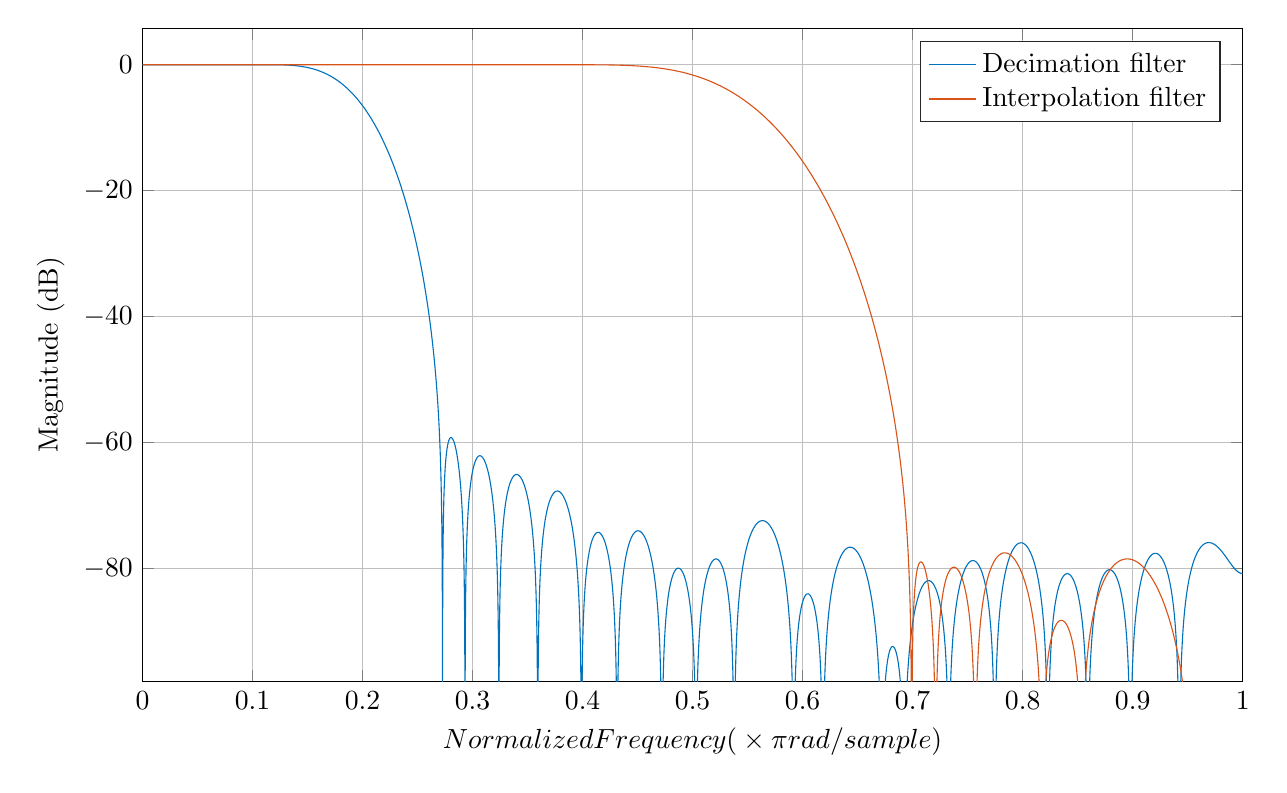
\begin{tikzpicture}

\begin{axis}[%
width=5.5in,
height=3.267in,
at={(1.281in,0.441in)},
scale only axis,
unbounded coords=jump,
xmin=0,
xmax=0.9998779296875,
xlabel={$\text{Normalized Frequency (}\times\pi\text{ rad/sample)}$},
xmajorgrids,
ymin=-97.9178075189385,
ymax=5.80114908390536,
ylabel={Magnitude (dB)},
ymajorgrids,
axis background/.style={fill=white},
legend style={legend cell align=left,align=left,draw=white!15!black}
]
\addplot [color=mycolor1,solid,forget plot]
  table[row sep=crcr]{%
0	0.002385323281203\\
0.0001220703125	0.00238515620543467\\
0.000244140625	0.00238465500069651\\
0.0003662109375	0.00238381973514379\\
0.00048828125	0.00238265052200859\\
0.0006103515625	0.00238114752011143\\
0.000732421875	0.00237931093340649\\
0.0008544921875	0.00237714101120901\\
0.0009765625	0.00237463804796789\\
0.0010986328125	0.00237180238360679\\
0.001220703125	0.00236863440289881\\
0.0013427734375	0.00236513453592124\\
0.00146484375	0.00236130325782824\\
0.0015869140625	0.00235714108868024\\
0.001708984375	0.00235264859355766\\
0.0018310546875	0.00234782638233355\\
0.001953125	0.00234267510978725\\
0.0020751953125	0.0023371954752065\\
0.002197265625	0.00233138822267165\\
0.0023193359375	0.00232525414077145\\
0.00244140625	0.00231879406231883\\
0.0025634765625	0.00231200886469196\\
0.002685546875	0.00230489946932266\\
0.0028076171875	0.00229746684169641\\
0.0029296875	0.00228971199135231\\
0.0030517578125	0.00228163597159892\\
0.003173828125	0.00227323987945738\\
0.0032958984375	0.00226452485554773\\
0.00341796875	0.00225549208369102\\
0.0035400390625	0.00224614279125035\\
0.003662109375	0.00223647824844875\\
0.0037841796875	0.00222649976865341\\
0.00390625	0.00221620870775041\\
0.0040283203125	0.00220560646437207\\
0.004150390625	0.00219469447961274\\
0.0042724609375	0.0021834742366309\\
0.00439453125	0.00217194726076286\\
0.0045166015625	0.002160115119068\\
0.004638671875	0.00214797942038558\\
0.0047607421875	0.00213554181482323\\
0.0048828125	0.0021228039938137\\
0.0050048828125	0.00210976768977389\\
0.005126953125	0.00209643467593423\\
0.0052490234375	0.00208280676594086\\
0.00537109375	0.00206888581396925\\
0.0054931640625	0.00205467371409895\\
0.005615234375	0.00204017240037047\\
0.0057373046875	0.0020253838462736\\
0.005859375	0.00201031006480434\\
0.0059814453125	0.00199495310783959\\
0.006103515625	0.00197931506625082\\
0.0062255859375	0.0019633980693925\\
0.00634765625	0.00194720428476103\\
0.0064697265625	0.00193073591810844\\
0.006591796875	0.00191399521258973\\
0.0067138671875	0.00189698444904707\\
0.0068359375	0.00187970594521403\\
0.0069580078125	0.00186216205582923\\
0.007080078125	0.00184435517201109\\
0.0072021484375	0.00182628772120097\\
0.00732421875	0.00180796216670842\\
0.0074462890625	0.0017893810073133\\
0.007568359375	0.00177054677726574\\
0.0076904296875	0.00175146204554721\\
0.0078125	0.00173212941587053\\
0.0079345703125	0.00171255152616823\\
0.008056640625	0.00169273104819467\\
0.0081787109375	0.00167267068746924\\
0.00830078125	0.0016523731825373\\
0.0084228515625	0.00163184130502714\\
0.008544921875	0.0016110778589109\\
0.0086669921875	0.00159008568039098\\
0.0087890625	0.00156886763744524\\
0.0089111328125	0.00154742662942908\\
0.009033203125	0.00152576558673445\\
0.0091552734375	0.00150388747044872\\
0.00927734375	0.00148179527189996\\
0.0093994140625	0.00145949201237272\\
0.009521484375	0.00143698074248277\\
0.0096435546875	0.00141426454212024\\
0.009765625	0.00139134651976747\\
0.0098876953125	0.00136822981221485\\
0.010009765625	0.00134491758416289\\
0.0101318359375	0.00132141302776745\\
0.01025390625	0.00129771936218503\\
0.0103759765625	0.00127383983328855\\
0.010498046875	0.00124977771315571\\
0.0106201171875	0.00122553629967115\\
0.0107421875	0.00120111891595798\\
0.0108642578125	0.0011765289102641\\
0.010986328125	0.00115176965510955\\
0.0111083984375	0.00112684454722967\\
0.01123046875	0.00110175700689297\\
0.0113525390625	0.00107651047756008\\
0.011474609375	0.00105110842537215\\
0.0115966796875	0.00102555433869611\\
0.01171875	0.000999851727783607\\
0.0118408203125	0.000974004124145722\\
0.011962890625	0.000948015080211917\\
0.0120849609375	0.000921888168818441\\
0.01220703125	0.000895626982753583\\
0.0123291015625	0.000869235134302926\\
0.012451171875	0.000842716254624065\\
0.0125732421875	0.000816073993576083\\
0.0126953125	0.000789312018923738\\
0.0128173828125	0.000762434016110092\\
0.012939453125	0.000735443687460702\\
0.0130615234375	0.000708344752126777\\
0.01318359375	0.000681140945175684\\
0.0133056640625	0.000653836017420417\\
0.013427734375	0.000626433734680631\\
0.0135498046875	0.000598937877441585\\
0.013671875	0.000571352240285705\\
0.0137939453125	0.000543680631437837\\
0.013916015625	0.000515926872139971\\
0.0140380859375	0.000488094796423866\\
0.01416015625	0.000460188250258398\\
0.0142822265625	0.000432211091322188\\
0.014404296875	0.000404167188264637\\
0.0145263671875	0.000376060420308022\\
0.0146484375	0.000347894676849592\\
0.0147705078125	0.000319673856722602\\
0.014892578125	0.000291401867798413\\
0.0150146484375	0.000263082626418054\\
0.01513671875	0.00023472005699432\\
0.0152587890625	0.000206318091272806\\
0.015380859375	0.000177880668047692\\
0.0155029296875	0.000149411732422777\\
0.015625	0.000120915235413577\\
0.0157470703125	9.23951334357298e-05\\
0.015869140625	6.38553876228798e-05\\
0.0159912109375	3.52999635424567e-05\\
0.01611328125	6.73283045671269e-06\\
0.0162353515625	-2.18420391888685e-05\\
0.016357421875	-5.04206701634757e-05\\
0.0164794921875	-7.89990851330913e-05\\
0.0166015625	-0.000107573305172082\\
0.0167236328125	-0.000136139350047415\\
0.016845703125	-0.000164693239241842\\
0.0169677734375	-0.00019323099201074\\
0.01708984375	-0.000221748628234764\\
0.0172119140625	-0.000250242168704062\\
0.017333984375	-0.000278707636027775\\
0.0174560546875	-0.000307141054690874\\
0.017578125	-0.000335538451963657\\
0.0177001953125	-0.000363895858299657\\
0.017822265625	-0.000392209307847224\\
0.0179443359375	-0.000420474839074814\\
0.01806640625	-0.000448688495225724\\
0.0181884765625	-0.000476846324943381\\
0.018310546875	-0.00050494438272608\\
0.0184326171875	-0.000532978729438582\\
0.0185546875	-0.000560945432937388\\
0.0186767578125	-0.000588840568696014\\
0.018798828125	-0.000616660220032372\\
0.0189208984375	-0.000644400478904572\\
0.01904296875	-0.000672057446479357\\
0.0191650390625	-0.000699627233359479\\
0.019287109375	-0.000727105960436347\\
0.0194091796875	-0.000754489759344779\\
0.01953125	-0.000781774772860899\\
0.0196533203125	-0.00080895715564111\\
0.019775390625	-0.00083603307444946\\
0.0198974609375	-0.000862998709010299\\
0.02001953125	-0.00088985025246302\\
0.0201416015625	-0.000916583911646285\\
0.020263671875	-0.00094319590800751\\
0.0203857421875	-0.00096968247771656\\
0.0205078125	-0.000996039872518395\\
0.0206298828125	-0.00102226436018782\\
0.020751953125	-0.0010483522248137\\
0.0208740234375	-0.00107429976765161\\
0.02099609375	-0.00110010330740806\\
0.0211181640625	-0.00112575918086577\\
0.021240234375	-0.00115126374339525\\
0.0213623046875	-0.00117661336929586\\
0.021484375	-0.0012018044526485\\
0.0216064453125	-0.00122683340742924\\
0.021728515625	-0.00125169666830516\\
0.0218505859375	-0.00127639069108909\\
0.02197265625	-0.001300911952967\\
0.0220947265625	-0.00132525695352115\\
0.022216796875	-0.00134942221467327\\
0.0223388671875	-0.00137340428153721\\
0.0224609375	-0.00139719972275998\\
0.0225830078125	-0.00142080513114706\\
0.022705078125	-0.0014442171239466\\
0.0228271484375	-0.00146743234347468\\
0.02294921875	-0.0014904474575701\\
0.0230712890625	-0.00151325916010592\\
0.023193359375	-0.00153586417133056\\
0.0233154296875	-0.00155825923854991\\
0.0234375	-0.00158044113641154\\
0.0235595703125	-0.00160240666741629\\
0.023681640625	-0.00162415266248672\\
0.0238037109375	-0.001645675981365\\
0.02392578125	-0.00166697351295397\\
0.0240478515625	-0.00168804217588558\\
0.024169921875	-0.00170887891908933\\
0.0242919921875	-0.00172948072201962\\
0.0244140625	-0.00174984459516736\\
0.0245361328125	-0.00176996758062842\\
0.024658203125	-0.00178984675221727\\
0.0247802734375	-0.00180947921643337\\
0.02490234375	-0.00182886211234745\\
0.0250244140625	-0.00184799261228363\\
0.025146484375	-0.00186686792238788\\
0.0252685546875	-0.001885485282628\\
0.025390625	-0.0019038419677031\\
0.0255126953125	-0.00192193528698681\\
0.025634765625	-0.00193976258526618\\
0.0257568359375	-0.00195732124313963\\
0.02587890625	-0.00197460867707377\\
0.0260009765625	-0.00199162234019923\\
0.026123046875	-0.00200835972248115\\
0.0262451171875	-0.00202481835128765\\
0.0263671875	-0.00204099579133299\\
0.0264892578125	-0.00205688964575756\\
0.026611328125	-0.00207249755578687\\
0.0267333984375	-0.00208781720164097\\
0.02685546875	-0.00210284630253454\\
0.0269775390625	-0.00211758261724526\\
0.027099609375	-0.00213202394439804\\
0.0272216796875	-0.0021461681228061\\
0.02734375	-0.00216001303186886\\
0.0274658203125	-0.00217355659185614\\
0.027587890625	-0.00218679676419242\\
0.0277099609375	-0.00219973155202524\\
0.02783203125	-0.00221235900016836\\
0.0279541015625	-0.00222467719572705\\
0.028076171875	-0.00223668426843915\\
0.0281982421875	-0.00224837839073189\\
0.0283203125	-0.00225975777811982\\
0.0284423828125	-0.0022708206897164\\
0.028564453125	-0.00228156542817715\\
0.0286865234375	-0.0022919903403249\\
0.02880859375	-0.0023020938172067\\
0.0289306640625	-0.0023118742944348\\
0.029052734375	-0.00232133025252779\\
0.0291748046875	-0.00233046021702421\\
0.029296875	-0.00233926275899421\\
0.0294189453125	-0.0023477364950395\\
0.029541015625	-0.00235588008769128\\
0.0296630859375	-0.00236369224552391\\
0.02978515625	-0.00237117172355283\\
0.0299072265625	-0.00237831732351879\\
0.030029296875	-0.0023851278937741\\
0.0301513671875	-0.00239160232990798\\
0.0302734375	-0.00239773957468969\\
0.0303955078125	-0.00240353861840958\\
0.030517578125	-0.00240899849904963\\
0.0306396484375	-0.00241411830245397\\
0.03076171875	-0.00241889716261312\\
0.0308837890625	-0.00242333426177765\\
0.031005859375	-0.0024274288305719\\
0.0311279296875	-0.00243118014827814\\
0.03125	-0.00243458754306403\\
0.0313720703125	-0.00243765039192567\\
0.031494140625	-0.00244036812108561\\
0.0316162109375	-0.00244274020593593\\
0.03173828125	-0.00244476617137934\\
0.0318603515625	-0.00244644559177232\\
0.031982421875	-0.00244777809115249\\
0.0321044921875	-0.002448763343466\\
0.0322265625	-0.00244940107251068\\
0.0323486328125	-0.00244969105204973\\
0.032470703125	-0.00244963310615276\\
0.0325927734375	-0.00244922710896844\\
0.03271484375	-0.00244847298506556\\
0.0328369140625	-0.00244737070943302\\
0.032958984375	-0.00244592030753665\\
0.0330810546875	-0.00244412185537612\\
0.033203125	-0.0024419754797691\\
0.0333251953125	-0.00243948135795335\\
0.033447265625	-0.00243663971821206\\
0.0335693359375	-0.00243345083941904\\
0.03369140625	-0.00242991505143664\\
0.0338134765625	-0.00242603273483155\\
0.033935546875	-0.00242180432132955\\
0.0340576171875	-0.00241723029330387\\
0.0341796875	-0.00241231118434371\\
0.0343017578125	-0.00240704757874255\\
0.034423828125	-0.00240144011183929\\
0.0345458984375	-0.00239548947007506\\
0.03466796875	-0.00238919639048163\\
0.0347900390625	-0.00238256166136352\\
0.034912109375	-0.00237558612161592\\
0.0350341796875	-0.00236827066112255\\
0.03515625	-0.00236061622064199\\
0.0352783203125	-0.0023526237915803\\
0.035400390625	-0.00234429441604789\\
0.0355224609375	-0.00233562918691632\\
0.03564453125	-0.00232662924753413\\
0.0357666015625	-0.00231729579178364\\
0.035888671875	-0.00230763006408097\\
0.0360107421875	-0.00229763335897815\\
0.0361328125	-0.00228730702150415\\
0.0362548828125	-0.00227665244659647\\
0.036376953125	-0.00226567107949904\\
0.0364990234375	-0.00225436441508009\\
0.03662109375	-0.00224273399823005\\
0.0367431640625	-0.00223078142346367\\
0.036865234375	-0.00221850833469261\\
0.0369873046875	-0.00220591642545287\\
0.037109375	-0.00219300743833628\\
0.0372314453125	-0.00217978316510425\\
0.037353515625	-0.00216624544640354\\
0.0374755859375	-0.00215239617165253\\
0.03759765625	-0.00213823727892759\\
0.0377197265625	-0.00212377075445147\\
0.037841796875	-0.00210899863299119\\
0.0379638671875	-0.00209392299706224\\
0.0380859375	-0.00207854597704227\\
0.0382080078125	-0.00206286975094372\\
0.038330078125	-0.0020468965441296\\
0.0384521484375	-0.00203062862914294\\
0.03857421875	-0.00201406832536577\\
0.0386962890625	-0.0019972179989054\\
0.038818359375	-0.00198008006236705\\
0.0389404296875	-0.00196265697445597\\
0.0390625	-0.00194495123980687\\
0.0391845703125	-0.00192696540869974\\
0.039306640625	-0.00190870207694616\\
0.0394287109375	-0.00189016388526397\\
0.03955078125	-0.00187135351933421\\
0.0396728515625	-0.00185227370934626\\
0.039794921875	-0.00183292722977058\\
0.0399169921875	-0.00181331689884701\\
0.0400390625	-0.00179344557864169\\
0.0401611328125	-0.00177331617442178\\
0.040283203125	-0.00175293163448487\\
0.0404052734375	-0.00173229494964744\\
0.04052734375	-0.00171140915324486\\
0.0406494140625	-0.00169027732044924\\
0.040771484375	-0.00166890256804209\\
0.0408935546875	-0.00164728805413006\\
0.041015625	-0.00162543697774709\\
0.0411376953125	-0.00160335257839961\\
0.041259765625	-0.00158103813578236\\
0.0413818359375	-0.00155849696932364\\
0.04150390625	-0.0015357324379579\\
0.0416259765625	-0.00151274793944367\\
0.041748046875	-0.00148954691024983\\
0.0418701171875	-0.00146613282504404\\
0.0419921875	-0.00144250919629485\\
0.0421142578125	-0.00141867957364639\\
0.042236328125	-0.00139464754391838\\
0.0423583984375	-0.00137041673031035\\
0.04248046875	-0.00134599079211739\\
0.0426025390625	-0.00132137342427541\\
0.042724609375	-0.00129656835684955\\
0.0428466796875	-0.00127157935469313\\
0.04296875	-0.00124641021693606\\
0.0430908203125	-0.00122106477641637\\
0.043212890625	-0.00119554689933921\\
0.0433349609375	-0.00116986048493573\\
0.04345703125	-0.00114400946455362\\
0.0435791015625	-0.00111799780154342\\
0.043701171875	-0.00109182949069009\\
0.0438232421875	-0.00106550855758769\\
0.0439453125	-0.00103903905829839\\
0.0440673828125	-0.00101242507867028\\
0.044189453125	-0.000985670733996358\\
0.0443115234375	-0.000958780168389239\\
0.04443359375	-0.000931757554269552\\
0.0445556640625	-0.000904607091854359\\
0.044677734375	-0.000877333008645564\\
0.0447998046875	-0.000849939558804635\\
0.044921875	-0.000822431022641013\\
0.0450439453125	-0.000794811706214205\\
0.045166015625	-0.000767085940424295\\
0.0452880859375	-0.000739258080955096\\
0.04541015625	-0.000711332507080442\\
0.0455322265625	-0.00068331362177787\\
0.045654296875	-0.000655205850591756\\
0.0457763671875	-0.000627013641349095\\
0.0458984375	-0.000598741463477381\\
0.0460205078125	-0.000570393807493019\\
0.046142578125	-0.000541975184319199\\
0.0462646484375	-0.000513490124717464\\
0.04638671875	-0.000484943178662434\\
0.0465087890625	-0.000456338914830212\\
0.046630859375	-0.000427681919916267\\
0.0467529296875	-0.000398976798010153\\
0.046875	-0.000370228170027076\\
0.0469970703125	-0.000341440672968929\\
0.047119140625	-0.000312618959469546\\
0.0472412109375	-0.000283767696998893\\
0.04736328125	-0.000254891567465165\\
0.0474853515625	-0.000225995266191603\\
0.047607421875	-0.000197083501632278\\
0.0477294921875	-0.000168160994633126\\
0.0478515625	-0.000139232477636142\\
0.0479736328125	-0.000110302694281472\\
0.048095703125	-8.13763983842364e-05\\
0.0482177734375	-5.24583537071521e-05\\
0.04833984375	-2.35533330510407e-05\\
0.0484619140625	5.33388254098099e-06\\
0.048583984375	3.41985040677173e-05\\
0.0487060546875	6.30357355930755e-05\\
0.048828125	9.18407747576566e-05\\
0.0489501953125	0.000120608813460876\\
0.049072265625	0.000149335038599929\\
0.0491943359375	0.000178014632695067\\
0.04931640625	0.000206642774685406\\
0.0494384765625	0.000235214640440518\\
0.049560546875	0.000263725403556236\\
0.0496826171875	0.000292170236036782\\
0.0498046875	0.000320544309147408\\
0.0499267578125	0.000348842793698623\\
0.050048828125	0.000377060861239897\\
0.0501708984375	0.000405193684400729\\
0.05029296875	0.000433236437800133\\
0.0504150390625	0.000461184298558237\\
0.050537109375	0.00048903244731946\\
0.0506591796875	0.000516776068593572\\
0.05078125	0.000544410351835722\\
0.0509033203125	0.000571930491730654\\
0.051025390625	0.000599331689386418\\
0.0511474609375	0.000626609152618585\\
0.05126953125	0.00065375809708712\\
0.0513916015625	0.000680773746580599\\
0.051513671875	0.000707651334039383\\
0.0516357421875	0.000734386102294593\\
0.0517578125	0.00076097330452285\\
0.0518798828125	0.000787408205326301\\
0.052001953125	0.00081368608101684\\
0.0521240234375	0.000839802220866659\\
0.05224609375	0.000865751927392466\\
0.0523681640625	0.000891530517378669\\
0.052490234375	0.00091713332233212\\
0.0526123046875	0.000942555689618985\\
0.052734375	0.000967792982635274\\
0.0528564453125	0.000992840582057397\\
0.052978515625	0.00101769388629691\\
0.0531005859375	0.00104234831229633\\
0.05322265625	0.00106679929626807\\
0.0533447265625	0.00109104229443346\\
0.053466796875	0.00111507278364797\\
0.0535888671875	0.00113888626236758\\
0.0537109375	0.00116247825098981\\
0.0538330078125	0.00118584429316115\\
0.053955078125	0.00120897995577707\\
0.0540771484375	0.00123188083051673\\
0.05419921875	0.00125454253378621\\
0.0543212890625	0.00127696070802585\\
0.054443359375	0.00129913102216506\\
0.0545654296875	0.00132104917247489\\
0.0546875	0.00134271088313653\\
0.0548095703125	0.0013641119071508\\
0.054931640625	0.00138524802679285\\
0.0550537109375	0.00140611505469224\\
0.05517578125	0.00142670883428764\\
0.0552978515625	0.00144702524062268\\
0.055419921875	0.00146706018114173\\
0.0555419921875	0.00148680959614467\\
0.0556640625	0.00150626945986687\\
0.0557861328125	0.00152543578087716\\
0.055908203125	0.00154430460304411\\
0.0560302734375	0.00156287200599081\\
0.05615234375	0.00158113410600436\\
0.0562744140625	0.00159908705660428\\
0.056396484375	0.00161672704928151\\
0.0565185546875	0.00163405031435104\\
0.056640625	0.00165105312134983\\
0.0567626953125	0.00166773177994628\\
0.056884765625	0.00168408264056552\\
0.0570068359375	0.00170010209512839\\
0.05712890625	0.00171578657767668\\
0.0572509765625	0.00173113256499846\\
0.057373046875	0.00174613657748068\\
0.0574951171875	0.00176079517967764\\
0.0576171875	0.00177510498087941\\
0.0577392578125	0.00178906263596446\\
0.057861328125	0.00180266484602498\\
0.0579833984375	0.00181590835899215\\
0.05810546875	0.00182878997020453\\
0.0582275390625	0.00184130652326076\\
0.058349609375	0.00185345491053113\\
0.0584716796875	0.00186523207378286\\
0.05859375	0.00187663500503277\\
0.0587158203125	0.0018876607467746\\
0.058837890625	0.00189830639317279\\
0.0589599609375	0.00190856909023296\\
0.05908203125	0.00191844603648406\\
0.0592041015625	0.00192793448394468\\
0.059326171875	0.00193703173829363\\
0.0594482421875	0.00194573515977936\\
0.0595703125	0.00195404216373163\\
0.0596923828125	0.00196195022118673\\
0.059814453125	0.00196945685939909\\
0.0599365234375	0.00197655966246657\\
0.06005859375	0.00198325627212625\\
0.0601806640625	0.00198954438798182\\
0.060302734375	0.00199542176835621\\
0.0604248046875	0.0020008862306895\\
0.060546875	0.00200593565227791\\
0.0606689453125	0.00201056797067167\\
0.060791015625	0.00201478118435716\\
0.0609130859375	0.00201857335315481\\
0.06103515625	0.00202194259884436\\
0.0611572265625	0.00202488710584703\\
0.061279296875	0.00202740512150967\\
0.0614013671875	0.00202949495678695\\
0.0615234375	0.00203115498663919\\
0.0616455078125	0.00203238365065772\\
0.061767578125	0.00203317945351955\\
0.0618896484375	0.00203354096555586\\
0.06201171875	0.00203346682309302\\
0.0621337890625	0.00203295572913476\\
0.062255859375	0.00203200645358947\\
0.0623779296875	0.00203061783400926\\
0.0625	0.00202878877593093\\
0.0626220703125	0.00202651825327393\\
0.062744140625	0.00202380530885193\\
0.0628662109375	0.00202064905494126\\
0.06298828125	0.00201704867345143\\
0.0631103515625	0.00201300341655042\\
0.063232421875	0.00200851260700574\\
0.0633544921875	0.00200357563875286\\
0.0634765625	0.00199819197706574\\
0.0635986328125	0.00199236115901158\\
0.063720703125	0.00198608279401924\\
0.0638427734375	0.00197935656410664\\
0.06396484375	0.00197218222416495\\
0.0640869140625	0.00196455960264075\\
0.064208984375	0.00195648860153597\\
0.0643310546875	0.00194796919709006\\
0.064453125	0.00193900143972314\\
0.0645751953125	0.00192958545477495\\
0.064697265625	0.00191972144267538\\
0.0648193359375	0.00190940967911502\\
0.06494140625	0.00189865051549987\\
0.0650634765625	0.00188744437934929\\
0.065185546875	0.00187579177429598\\
0.0653076171875	0.00186369328065439\\
0.0654296875	0.00185114955553445\\
0.0655517578125	0.00183816133312575\\
0.065673828125	0.00182472942503864\\
0.0657958984375	0.00181085472036102\\
0.06591796875	0.00179653818616998\\
0.0660400390625	0.00178178086741809\\
0.066162109375	0.00176658388744499\\
0.0662841796875	0.00175094844803425\\
0.06640625	0.00173487582969756\\
0.0665283203125	0.00171836739173159\\
0.066650390625	0.00170142457255906\\
0.0667724609375	0.00168404888978557\\
0.06689453125	0.00166624194025644\\
0.0670166015625	0.00164800540056831\\
0.067138671875	0.00162934102678491\\
0.0672607421875	0.001610250654835\\
0.0673828125	0.00159073620051231\\
0.0675048828125	0.00157079965964613\\
0.067626953125	0.00155044310815811\\
0.0677490234375	0.00152966870211912\\
0.06787109375	0.00150847867797665\\
0.0679931640625	0.00148687535238423\\
0.068115234375	0.00146486112248567\\
0.0682373046875	0.00144243846574454\\
0.068359375	0.00141960994017154\\
0.0684814453125	0.00139637818426763\\
0.068603515625	0.00137274591702408\\
0.0687255859375	0.00134871593786556\\
0.06884765625	0.00132429112682075\\
0.0689697265625	0.00129947444435174\\
0.069091796875	0.00127426893124039\\
0.0692138671875	0.00124867770887249\\
0.0693359375	0.0012227039787831\\
0.0694580078125	0.00119635102288385\\
0.069580078125	0.00116962220323558\\
0.0697021484375	0.00114252096210521\\
0.06982421875	0.00111505082162466\\
0.0699462890625	0.00108721538390455\\
0.070068359375	0.00105901833080679\\
0.0701904296875	0.0010304634238878\\
0.0703125	0.00100155450411421\\
0.0704345703125	0.000972295491806108\\
0.070556640625	0.000942690386523282\\
0.0706787109375	0.000912743266667349\\
0.07080078125	0.000882458289595434\\
0.0709228515625	0.00085183969110858\\
0.071044921875	0.000820891785451749\\
0.0711669921875	0.00078961896497276\\
0.0712890625	0.000758025699894915\\
0.0714111328125	0.000726116538203314\\
0.071533203125	0.000693896105076419\\
0.0716552734375	0.000661369102886056\\
0.07177734375	0.000628540310856351\\
0.0718994140625	0.000595414584665832\\
0.072021484375	0.000561996856163205\\
0.0721435546875	0.000528292133026298\\
0.072265625	0.00049430549859153\\
0.0723876953125	0.000460042111228631\\
0.072509765625	0.000425507204170117\\
0.0726318359375	0.000390706085056536\\
0.07275390625	0.000355644135595412\\
0.0728759765625	0.000320326811163341\\
0.072998046875	0.000284759640237553\\
0.0731201171875	0.000248948224225387\\
0.0732421875	0.000212898236725323\\
0.0733642578125	0.000176615423470139\\
0.073486328125	0.000140105601417417\\
0.0736083984375	0.000103374658579014\\
0.07373046875	6.64285533957809e-05\\
0.0738525390625	2.92733142828183e-05\\
0.073974609375	-8.08496088211541e-06\\
0.0740966796875	-4.56401052701949e-05\\
0.07421875	-8.33858838404922e-05\\
0.0743408203125	-0.000121315993510507\\
0.074462890625	-0.000159424064122504\\
0.0745849609375	-0.000197703658841419\\
0.07470703125	-0.000236148274609604\\
0.0748291015625	-0.000274751343056323\\
0.074951171875	-0.000313506230952498\\
0.0750732421875	-0.000352406240779146\\
0.0751953125	-0.000391444611466341\\
0.0753173828125	-0.000430614519132178\\
0.075439453125	-0.000469909077594366\\
0.0755615234375	-0.000509321339052349\\
0.07568359375	-0.000548844295053641\\
0.0758056640625	-0.000588470876778047\\
0.075927734375	-0.000628193956117684\\
0.0760498046875	-0.000668006346359107\\
0.076171875	-0.000707900802694894\\
0.0762939453125	-0.000747870023303676\\
0.076416015625	-0.000787906649861725\\
0.0765380859375	-0.000828003268622979\\
0.07666015625	-0.000868152410930634\\
0.0767822265625	-0.000908346554126638\\
0.076904296875	-0.000948578122518029\\
0.0770263671875	-0.000988839488059057\\
0.0771484375	-0.00102912297126068\\
0.0772705078125	-0.0010694208420432\\
0.077392578125	-0.00110972532075948\\
0.0775146484375	-0.00115002857882018\\
0.07763671875	-0.00119032273977382\\
0.0777587890625	-0.00123059988032992\\
0.077880859375	-0.00127085203104116\\
0.0780029296875	-0.00131107117738338\\
0.078125	-0.00135124926077879\\
0.0782470703125	-0.00139137817944857\\
0.078369140625	-0.00143144978949294\\
0.0784912109375	-0.00147145590585751\\
0.07861328125	-0.0015113883033564\\
0.0787353515625	-0.00155123871752494\\
0.078857421875	-0.00159099884609759\\
0.0789794921875	-0.00163066034951953\\
0.0791015625	-0.00167021485236774\\
0.0792236328125	-0.00170965394437417\\
0.079345703125	-0.00174896918139211\\
0.0794677734375	-0.00178815208670358\\
0.07958984375	-0.00182719415187194\\
0.0797119140625	-0.00186608683804934\\
0.079833984375	-0.00190482157717042\\
0.0799560546875	-0.00194338977286179\\
0.080078125	-0.00198178280186312\\
0.0802001953125	-0.00201999201510716\\
0.080322265625	-0.00205800873891349\\
0.0804443359375	-0.00209582427612531\\
0.08056640625	-0.00213342990741694\\
0.0806884765625	-0.00217081689254428\\
0.080810546875	-0.00220797647153859\\
0.0809326171875	-0.00224489986584331\\
0.0810546875	-0.00228157827979203\\
0.0811767578125	-0.00231800290191586\\
0.081298828125	-0.00235416490585294\\
0.0814208984375	-0.00239005545216742\\
0.08154296875	-0.00242566568914526\\
0.0816650390625	-0.00246098675472695\\
0.081787109375	-0.00249600977713271\\
0.0819091796875	-0.00253072587696579\\
0.08203125	-0.00256512616783766\\
0.0821533203125	-0.00259920175841444\\
0.082275390625	-0.00263294375332634\\
0.0823974609375	-0.00266634325481618\\
0.08251953125	-0.00269939136398989\\
0.0826416015625	-0.00273207918240814\\
0.082763671875	-0.00276439781345061\\
0.0828857421875	-0.00279633836362336\\
0.0830078125	-0.00282789194426414\\
0.0831298828125	-0.00285904967284978\\
0.083251953125	-0.00288980267453098\\
0.0833740234375	-0.0029201420835534\\
0.08349609375	-0.00295005904484924\\
0.0836181640625	-0.00297954471562889\\
0.083740234375	-0.00300859026663147\\
0.0838623046875	-0.00303718688388699\\
0.083984375	-0.00306532577019425\\
0.0841064453125	-0.00309299814676933\\
0.084228515625	-0.00312019525466667\\
0.0843505859375	-0.00314690835637066\\
0.08447265625	-0.00317312873755782\\
0.0845947265625	-0.00319884770851786\\
0.084716796875	-0.003224056605859\\
0.0848388671875	-0.00324874679409959\\
0.0849609375	-0.00327290966720284\\
0.0850830078125	-0.00329653665045271\\
0.085205078125	-0.0033196192019318\\
0.0853271484375	-0.00334214881422668\\
0.08544921875	-0.00336411701607631\\
0.0855712890625	-0.00338551537407739\\
0.085693359375	-0.00340633549444647\\
0.0858154296875	-0.00342656902449789\\
0.0859375	-0.00344620765469017\\
0.0860595703125	-0.00346524312004703\\
0.086181640625	-0.00348366720209015\\
0.0863037109375	-0.00350147173048754\\
0.08642578125	-0.00351864858464523\\
0.0865478515625	-0.00353518969592415\\
0.086669921875	-0.00355108704889062\\
0.0867919921875	-0.00356633268341966\\
0.0869140625	-0.00358091869634336\\
0.0870361328125	-0.00359483724326992\\
0.087158203125	-0.00360808054051631\\
0.0872802734375	-0.00362064086664304\\
0.08740234375	-0.00363251056455738\\
0.0875244140625	-0.00364368204310495\\
0.087646484375	-0.0036541477791161\\
0.0877685546875	-0.00366390031905439\\
0.087890625	-0.00367293228111976\\
0.0880126953125	-0.00368123635672646\\
0.088134765625	-0.00368880531289051\\
0.0882568359375	-0.00369563199348022\\
0.08837890625	-0.00370170932177416\\
0.0885009765625	-0.00370703030171171\\
0.088623046875	-0.00371158802028049\\
0.0887451171875	-0.0037153756491648\\
0.0888671875	-0.00371838644673517\\
0.0889892578125	-0.00372061375998101\\
0.089111328125	-0.00372205102627277\\
0.0892333984375	-0.00372269177557882\\
0.08935546875	-0.00372252963228448\\
0.0894775390625	-0.00372155831695409\\
0.089599609375	-0.00371977164854798\\
0.0897216796875	-0.00371716354618457\\
0.08984375	-0.00371372803135728\\
0.0899658203125	-0.00370945922952615\\
0.090087890625	-0.0037043513724484\\
0.0902099609375	-0.00369839879994061\\
0.09033203125	-0.00369159596198188\\
0.0904541015625	-0.00368393742064654\\
0.090576171875	-0.00367541785203684\\
0.0906982421875	-0.00366603204861349\\
0.0908203125	-0.00365577492061675\\
0.0909423828125	-0.00364464149868127\\
0.091064453125	-0.00363262693542765\\
0.0911865234375	-0.00361972650779308\\
0.09130859375	-0.00360593561873657\\
0.0914306640625	-0.0035912497995696\\
0.091552734375	-0.00357566471188875\\
0.0916748046875	-0.00355917614939472\\
0.091796875	-0.00354178004027972\\
0.0919189453125	-0.00352347244916018\\
0.092041015625	-0.00350424957895257\\
0.0921630859375	-0.00348410777314712\\
0.09228515625	-0.00346304351774052\\
0.0924072265625	-0.00344105344333911\\
0.092529296875	-0.00341813432726212\\
0.0926513671875	-0.00339428309553114\\
0.0927734375	-0.00336949682480281\\
0.0928955078125	-0.00334377274492681\\
0.093017578125	-0.00331710824036691\\
0.0931396484375	-0.00328950085275892\\
0.09326171875	-0.00326094828290024\\
0.0933837890625	-0.00323144839256884\\
0.093505859375	-0.00320099920696748\\
0.0936279296875	-0.00316959891654278\\
0.09375	-0.00313724587914521\\
0.0938720703125	-0.00310393862218916\\
0.093994140625	-0.00306967584458562\\
0.0941162109375	-0.0030344564190159\\
0.09423828125	-0.00299827939386432\\
0.0943603515625	-0.00296114399543512\\
0.094482421875	-0.00292304962982826\\
0.0946044921875	-0.00288399588538368\\
0.0947265625	-0.00284398253438667\\
0.0948486328125	-0.00280300953539836\\
0.094970703125	-0.00276107703524531\\
0.0950927734375	-0.00271818537123636\\
0.09521484375	-0.00267433507303849\\
0.0953369140625	-0.00262952686495055\\
0.095458984375	-0.00258376166800645\\
0.0955810546875	-0.00253704060179416\\
0.095703125	-0.00248936498684316\\
0.0958251953125	-0.00244073634655706\\
0.095947265625	-0.00239115640948739\\
0.0960693359375	-0.00234062711098204\\
0.09619140625	-0.00228915059580004\\
0.0963134765625	-0.00223672921976004\\
0.096435546875	-0.00218336555212773\\
0.0965576171875	-0.00212906237749166\\
0.0966796875	-0.00207382269786649\\
0.0968017578125	-0.00201764973479612\\
0.096923828125	-0.00196054693151382\\
0.0970458984375	-0.00190251795481799\\
0.09716796875	-0.00184356669723229\\
0.0972900390625	-0.00178369727905192\\
0.097412109375	-0.00172291405039005\\
0.0975341796875	-0.00166122159333781\\
0.09765625	-0.00159862472372652\\
0.0977783203125	-0.00153512849357185\\
0.097900390625	-0.00147073819266552\\
0.0980224609375	-0.00140545935101954\\
0.09814453125	-0.00133929774062835\\
0.0982666015625	-0.00127225937757203\\
0.098388671875	-0.00120435052411949\\
0.0985107421875	-0.00113557769060435\\
0.0986328125	-0.00106594763758494\\
0.0987548828125	-0.000995467377606474\\
0.098876953125	-0.000924144177531616\\
0.0989990234375	-0.000851985560302637\\
0.09912109375	-0.000778999307044614\\
0.0992431640625	-0.000705193458884423\\
0.099365234375	-0.000630576319167631\\
0.0994873046875	-0.00055515645522064\\
0.099609375	-0.000478942700510743\\
0.0997314453125	-0.000401944156408263\\
0.099853515625	-0.000324170194176077\\
0.0999755859375	-0.000245630457186508\\
0.10009765625	-0.00016633486234241\\
0.1002197265625	-8.62936025782801e-05\\
0.100341796875	-5.51714839502893e-06\\
0.1004638671875	7.59837502073424e-05\\
0.1005859375	0.000158198061512849\\
0.1007080078125	0.000241114470554749\\
0.100830078125	0.000324721377012338\\
0.1009521484375	0.000409006893335118\\
0.10107421875	0.000493958842923803\\
0.1011962890625	0.000579564758254492\\
0.101318359375	0.000665811879116518\\
0.1014404296875	0.000752687150452402\\
0.1015625	0.00084017722082308\\
0.1016845703125	0.000928268440475222\\
0.101806640625	0.00101694685952225\\
0.1019287109375	0.0011061982260685\\
0.10205078125	0.00119600798439023\\
0.1021728515625	0.00128636127340087\\
0.102294921875	0.00137724292443409\\
0.1024169921875	0.00146863745993642\\
0.1025390625	0.00156052909119353\\
0.1026611328125	0.0016529017171365\\
0.102783203125	0.00174573892201124\\
0.1029052734375	0.00183902397418478\\
0.10302734375	0.00193273982398523\\
0.1031494140625	0.00202686910239436\\
0.103271484375	0.00212139411883072\\
0.1033935546875	0.00221629686006963\\
0.103515625	0.00231155898802626\\
0.1036376953125	0.0024071618383914\\
0.103759765625	0.00250308641886932\\
0.1038818359375	0.00259931340764297\\
0.10400390625	0.00269582315155503\\
0.1041259765625	0.00279259566462997\\
0.104248046875	0.00288961062636872\\
0.1043701171875	0.00298684738027077\\
0.1044921875	0.00308428493218571\\
0.1046142578125	0.00318190194872159\\
0.104736328125	0.00327967675559648\\
0.1048583984375	0.00337758733644478\\
0.10498046875	0.00347561133077079\\
0.1051025390625	0.00357372603286876\\
0.105224609375	0.00367190839011755\\
0.1053466796875	0.00377013500138901\\
0.10546875	0.00386838211585427\\
0.1055908203125	0.00396662563122163\\
0.105712890625	0.00406484109248595\\
0.1058349609375	0.00416300369045075\\
0.10595703125	0.00426108826019345\\
0.1060791015625	0.00435906927975793\\
0.106201171875	0.00445692086867666\\
0.1063232421875	0.00455461678677693\\
0.1064453125	0.00465213043247559\\
0.1065673828125	0.00474943484186952\\
0.106689453125	0.00484650268697351\\
0.1068115234375	0.00494330627458339\\
0.10693359375	0.00503981754502547\\
0.1070556640625	0.00513600807079229\\
0.107177734375	0.00523184905523522\\
0.1072998046875	0.00532731133137077\\
0.107421875	0.00542236536045948\\
0.1075439453125	0.0055169812311533\\
0.107666015625	0.00561112865773339\\
0.1077880859375	0.0057047769794849\\
0.10791015625	0.00579789515904849\\
0.1080322265625	0.00589045178151082\\
0.108154296875	0.005982415053154\\
0.1082763671875	0.0060737528002619\\
0.1083984375	0.00616443246821063\\
0.1085205078125	0.00625442112016117\\
0.108642578125	0.0063436854359793\\
0.1087646484375	0.00643219171121245\\
0.10888671875	0.00651990585618023\\
0.1090087890625	0.00660679339466697\\
0.109130859375	0.00669281946295541\\
0.1092529296875	0.00677794880903093\\
0.109375	0.00686214579144462\\
0.1094970703125	0.00694537437817644\\
0.109619140625	0.00702759814600995\\
0.1097412109375	0.00710878027933859\\
0.10986328125	0.00718888356931302\\
0.1099853515625	0.00726787041315902\\
0.110107421875	0.00734570281281322\\
0.1102294921875	0.00742234237446837\\
0.1103515625	0.00749775030755018\\
0.1104736328125	0.0075718874239783\\
0.110595703125	0.00764471413720003\\
0.1107177734375	0.00771619046156502\\
0.11083984375	0.00778627601130211\\
0.1109619140625	0.00785493000012139\\
0.111083984375	0.00792211124002051\\
0.1112060546875	0.00798777814100049\\
0.111328125	0.00805188871004248\\
0.1114501953125	0.00811440055048251\\
0.111572265625	0.0081752708614431\\
0.1116943359375	0.0082344564370942\\
0.11181640625	0.00829191366608484\\
0.1119384765625	0.00834759853069045\\
0.112060546875	0.00840146660658547\\
0.1121826171875	0.00845347306199074\\
0.1123046875	0.008503572657105\\
0.1124267578125	0.00855171974370705\\
0.112548828125	0.00859786826464415\\
0.1126708984375	0.00864197175303616\\
0.11279296875	0.00868398333216192\\
0.1129150390625	0.00872385571466339\\
0.113037109375	0.00876154120237516\\
0.1131591796875	0.0087969916856423\\
0.11328125	0.008830158643093\\
0.1134033203125	0.00886099314107014\\
0.113525390625	0.0088894458334039\\
0.1136474609375	0.00891546696095702\\
0.11376953125	0.00893900635128375\\
0.1138916015625	0.00896001341845931\\
0.114013671875	0.0089784371625683\\
0.1141357421875	0.00899422616942047\\
0.1142578125	0.00900732861049391\\
0.1143798828125	0.00901769224248028\\
0.114501953125	0.00902526440722795\\
0.1146240234375	0.00902999203128729\\
0.11474609375	0.00903182162602434\\
0.1148681640625	0.0090306992871092\\
0.114990234375	0.00902657069474344\\
0.1151123046875	0.00901938111320533\\
0.115234375	0.00900907539084983\\
0.1153564453125	0.00899559796005178\\
0.115478515625	0.00897889283703535\\
0.1156005859375	0.00895890362193086\\
0.11572265625	0.00893557349854746\\
0.1158447265625	0.00890884523465729\\
0.115966796875	0.00887866118165448\\
0.1160888671875	0.00884496327472561\\
0.1162109375	0.00880769303290663\\
0.1163330078125	0.00876679155908278\\
0.116455078125	0.00872219954010234\\
0.1165771484375	0.00867385724689029\\
0.11669921875	0.00862170453433464\\
0.1168212890625	0.00856568084179798\\
0.116943359375	0.00850572519283332\\
0.1170654296875	0.00844177619569564\\
0.1171875	0.00837377204339873\\
0.1173095703125	0.00830165051382892\\
0.117431640625	0.00822534897008609\\
0.1175537109375	0.00814480436071108\\
0.11767578125	0.00805995321974251\\
0.1177978515625	0.00797073166728524\\
0.117919921875	0.0078770754097377\\
0.1180419921875	0.00777891973979195\\
0.1181640625	0.00767619953728627\\
0.1182861328125	0.00756884926903467\\
0.118408203125	0.00745680298950901\\
0.1185302734375	0.0073399943411232\\
0.11865234375	0.00721835655474479\\
0.1187744140625	0.00709182244980866\\
0.118896484375	0.00696032443505601\\
0.1190185546875	0.00682379450898907\\
0.119140625	0.00668216426009849\\
0.1192626953125	0.00653536486754547\\
0.119384765625	0.00638332710155964\\
0.1195068359375	0.00622598132417806\\
0.11962890625	0.00606325748941572\\
0.1197509765625	0.00589508514417503\\
0.119873046875	0.00572139342864375\\
0.1199951171875	0.00554211107697711\\
0.1201171875	0.00535716641775252\\
0.1202392578125	0.00516648737482228\\
0.120361328125	0.00497000146776827\\
0.1204833984375	0.00476763581264095\\
0.12060546875	0.00455931712258462\\
0.1207275390625	0.00434497170874693\\
0.120849609375	0.00412452548061992\\
0.1209716796875	0.00389790394712008\\
0.12109375	0.00366503221715675\\
0.1212158203125	0.00342583500025739\\
0.121337890625	0.00318023660781819\\
0.1214599609375	0.00292816095327453\\
0.12158203125	0.00266953155346528\\
0.1217041015625	0.00240427152903067\\
0.121826171875	0.00213230360566286\\
0.1219482421875	0.00185355011450383\\
0.1220703125	0.00156793299345281\\
0.1221923828125	0.00127537378779152\\
0.122314453125	0.000975793651093682\\
0.1224365234375	0.000669113346361883\\
0.12255859375	0.000355253246652865\\
0.1226806640625	3.41333363849117e-05\\
0.122802734375	-0.000294326788093713\\
0.1229248046875	-0.000630207917197367\\
0.123046875	-0.000973591227250381\\
0.1231689453125	-0.00132455827940703\\
0.123291015625	-0.00168319101874204\\
0.1234130859375	-0.00204957177311371\\
0.12353515625	-0.00242378325219761\\
0.1236572265625	-0.00280590854612228\\
0.123779296875	-0.00319603112490086\\
0.1239013671875	-0.00359423483689625\\
0.1240234375	-0.00400060390785484\\
0.1241455078125	-0.00441522293976959\\
0.124267578125	-0.00483817690985688\\
0.1243896484375	-0.00526955116919225\\
0.12451171875	-0.00570943144168723\\
0.1246337890625	-0.00615790382295245\\
0.124755859375	-0.00661505477881974\\
0.1248779296875	-0.00708097114454631\\
0.125	-0.00755574012327997\\
0.1251220703125	-0.00803944928492228\\
0.125244140625	-0.00853218656493482\\
0.1253662109375	-0.00903404026297494\\
0.12548828125	-0.00954509904181577\\
0.1256103515625	-0.0100654519256977\\
0.125732421875	-0.0105951882995328\\
0.1258544921875	-0.0111343979070853\\
0.1259765625	-0.0116831708500627\\
0.1260986328125	-0.0122415975865806\\
0.126220703125	-0.0128097689297419\\
0.1263427734375	-0.0133877760464998\\
0.12646484375	-0.0139757104561795\\
0.1265869140625	-0.0145736640290011\\
0.126708984375	-0.015181728984885\\
0.1268310546875	-0.0157999978919179\\
0.126953125	-0.0164285636649879\\
0.1270751953125	-0.0170675195643071\\
0.127197265625	-0.0177169591940469\\
0.1273193359375	-0.0183769765008606\\
0.12744140625	-0.0190476657724048\\
0.1275634765625	-0.019729121635919\\
0.127685546875	-0.020421439056804\\
0.1278076171875	-0.021124713336917\\
0.1279296875	-0.0218390401133775\\
0.1280517578125	-0.0225645153568053\\
0.128173828125	-0.0233012353698427\\
0.1282958984375	-0.0240492967859609\\
0.12841796875	-0.0248087965673562\\
0.1285400390625	-0.0255798320038707\\
0.128662109375	-0.0263625007113433\\
0.1287841796875	-0.0271569006297909\\
0.12890625	-0.027963130022215\\
0.1290283203125	-0.028781287472782\\
0.129150390625	-0.0296114718852891\\
0.1292724609375	-0.0304537824815725\\
0.12939453125	-0.0313083187999723\\
0.1295166015625	-0.0321751806936845\\
0.129638671875	-0.0330544683289418\\
0.1297607421875	-0.0339462821838197\\
0.1298828125	-0.0348507230461905\\
0.1300048828125	-0.0357678920122453\\
0.130126953125	-0.036697890484902\\
0.1302490234375	-0.0376408201721574\\
0.13037109375	-0.0385967830851541\\
0.1304931640625	-0.039565881536987\\
0.130615234375	-0.0405482181405432\\
0.1307373046875	-0.0415438958070808\\
0.130859375	-0.0425530177446376\\
0.1309814453125	-0.0435756874560411\\
0.131103515625	-0.0446120087373743\\
0.1312255859375	-0.0456620856763266\\
0.13134765625	-0.0467260226504891\\
0.1314697265625	-0.0478039243253079\\
0.131591796875	-0.0488958956528904\\
0.1317138671875	-0.0500020418697886\\
0.1318359375	-0.0511224684956915\\
0.1319580078125	-0.0522572813312649\\
0.132080078125	-0.053406586456731\\
0.1322021484375	-0.0545704902299917\\
0.13232421875	-0.0557490992849239\\
0.1324462890625	-0.0569425205295602\\
0.132568359375	-0.0581508611443269\\
0.1326904296875	-0.0593742285803955\\
0.1328125	-0.0606127305577502\\
0.1329345703125	-0.0618664750635389\\
0.133056640625	-0.063135570350255\\
0.1331787109375	-0.0644201249339176\\
0.13330078125	-0.0657202475923668\\
0.1334228515625	-0.0670360473634446\\
0.133544921875	-0.0683676335432324\\
0.1336669921875	-0.0697151156840619\\
0.1337890625	-0.0710786035930937\\
0.1339111328125	-0.0724582073302145\\
0.134033203125	-0.0738540372063312\\
0.1341552734375	-0.0752662037814957\\
0.13427734375	-0.0766948178634266\\
0.1343994140625	-0.0781399905051217\\
0.134521484375	-0.0796018330036077\\
0.1346435546875	-0.0810804568978369\\
0.134765625	-0.0825759739669252\\
0.1348876953125	-0.0840884962284463\\
0.135009765625	-0.0856181359363859\\
0.1351318359375	-0.0871650055795499\\
0.13525390625	-0.0887292178796315\\
0.1353759765625	-0.0903108857895063\\
0.135498046875	-0.0919101224912993\\
0.1356201171875	-0.0935270413944522\\
0.1357421875	-0.0951617561343596\\
0.1358642578125	-0.0968143805699242\\
0.135986328125	-0.0984850287823065\\
0.1361083984375	-0.100173815072765\\
0.13623046875	-0.101880853960893\\
0.1363525390625	-0.103606260182858\\
0.136474609375	-0.105350148689638\\
0.1365966796875	-0.107112634644977\\
0.13671875	-0.108893833423906\\
0.1368408203125	-0.110693860610525\\
0.136962890625	-0.112512831996639\\
0.1370849609375	-0.114350863579546\\
0.13720703125	-0.116208071560322\\
0.1373291015625	-0.118084572342298\\
0.137451171875	-0.119980482528888\\
0.1375732421875	-0.12189591892178\\
0.1376953125	-0.123830998519509\\
0.1378173828125	-0.125785838515299\\
0.137939453125	-0.127760556295357\\
0.1380615234375	-0.129755269436998\\
0.13818359375	-0.131770095707111\\
0.1383056640625	-0.133805153060052\\
0.138427734375	-0.135860559636001\\
0.1385498046875	-0.137936433759137\\
0.138671875	-0.140032893935938\\
0.1387939453125	-0.14215005885319\\
0.138916015625	-0.144288047376392\\
0.1390380859375	-0.146446978547942\\
0.13916015625	-0.148626971585372\\
0.1392822265625	-0.150828145879359\\
0.139404296875	-0.153050620992303\\
0.1395263671875	-0.155294516656284\\
0.1396484375	-0.157559952771578\\
0.1397705078125	-0.159847049404448\\
0.139892578125	-0.162155926785886\\
0.1400146484375	-0.164486705309628\\
0.14013671875	-0.166839505530277\\
0.1402587890625	-0.169214448161824\\
0.140380859375	-0.171611654075889\\
0.1405029296875	-0.174031244299613\\
0.140625	-0.176473340014468\\
0.1407470703125	-0.178938062554153\\
0.140869140625	-0.181425533403058\\
0.1409912109375	-0.18393587419439\\
0.14111328125	-0.186469206708693\\
0.1412353515625	-0.189025652871862\\
0.141357421875	-0.191605334753774\\
0.1414794921875	-0.194208374566301\\
0.1416015625	-0.196834894661663\\
0.1417236328125	-0.19948501753106\\
0.141845703125	-0.202158865802573\\
0.1419677734375	-0.204856562239684\\
0.14208984375	-0.207578229739624\\
0.1422119140625	-0.210323991331791\\
0.142333984375	-0.213093970175919\\
0.1424560546875	-0.215888289560496\\
0.142578125	-0.218707072901111\\
0.1427001953125	-0.221550443739034\\
0.142822265625	-0.224418525739225\\
0.1429443359375	-0.227311442688972\\
0.14306640625	-0.230229318496129\\
0.1431884765625	-0.233172277187691\\
0.143310546875	-0.236140442908038\\
0.1434326171875	-0.239133939917338\\
0.1435546875	-0.24215289259007\\
0.1436767578125	-0.24519742541338\\
0.143798828125	-0.248267662985427\\
0.1439208984375	-0.251363730014077\\
0.14404296875	-0.254485751314974\\
0.1441650390625	-0.25763385181034\\
0.144287109375	-0.260808156527219\\
0.1444091796875	-0.264008790596051\\
0.14453125	-0.267235879248972\\
0.1446533203125	-0.270489547818556\\
0.144775390625	-0.273769921736175\\
0.1448974609375	-0.277077126530401\\
0.14501953125	-0.280411287825586\\
0.1451416015625	-0.283772531340503\\
0.145263671875	-0.287160982886689\\
0.1453857421875	-0.290576768366975\\
0.1455078125	-0.294020013774286\\
0.1456298828125	-0.297490845189714\\
0.145751953125	-0.300989388781488\\
0.1458740234375	-0.304515770803505\\
0.14599609375	-0.308070117593502\\
0.1461181640625	-0.311652555572209\\
0.146240234375	-0.315263211241529\\
0.1463623046875	-0.318902211183172\\
0.146484375	-0.322569682057576\\
0.1466064453125	-0.326265750602033\\
0.146728515625	-0.329990543629776\\
0.1468505859375	-0.333744188028334\\
0.14697265625	-0.33752681075822\\
0.1470947265625	-0.34133853885163\\
0.147216796875	-0.345179499411188\\
0.1473388671875	-0.349049819608354\\
0.1474609375	-0.352949626682459\\
0.1475830078125	-0.356879047939003\\
0.147705078125	-0.360838210748625\\
0.1478271484375	-0.364827242545857\\
0.14794921875	-0.368846270827532\\
0.1480712890625	-0.372895423151874\\
0.148193359375	-0.376974827136905\\
0.1483154296875	-0.381084610459538\\
0.1484375	-0.385224900853871\\
0.1485595703125	-0.389395826110558\\
0.148681640625	-0.393597514074997\\
0.1488037109375	-0.397830092646529\\
0.14892578125	-0.402093689776962\\
0.1490478515625	-0.406388433469601\\
0.149169921875	-0.410714451777949\\
0.1492919921875	-0.41507187280439\\
0.1494140625	-0.419460824699399\\
0.1495361328125	-0.423881435660007\\
0.149658203125	-0.428333833928889\\
0.1497802734375	-0.432818147793171\\
0.14990234375	-0.437334505583294\\
0.1500244140625	-0.441883035671879\\
0.150146484375	-0.446463866472584\\
0.1502685546875	-0.451077126439316\\
0.150390625	-0.455722944064632\\
0.1505126953125	-0.460401447879121\\
0.150634765625	-0.465112766450204\\
0.1507568359375	-0.469857028380886\\
0.15087890625	-0.474634362309132\\
0.1510009765625	-0.479444896906386\\
0.151123046875	-0.484288760876836\\
0.1512451171875	-0.489166082956388\\
0.1513671875	-0.494076991911527\\
0.1514892578125	-0.499021616538528\\
0.151611328125	-0.504000085662312\\
0.1517333984375	-0.509012528135543\\
0.15185546875	-0.514059072837711\\
0.1519775390625	-0.519139848674229\\
0.152099609375	-0.524254984575236\\
0.1522216796875	-0.529404609495089\\
0.15234375	-0.534588852411162\\
0.1524658203125	-0.539807842323057\\
0.152587890625	-0.545061708251524\\
0.1527099609375	-0.550350579238057\\
0.15283203125	-0.555674584343478\\
0.1529541015625	-0.561033852647427\\
0.153076171875	-0.566428513247331\\
0.1531982421875	-0.571858695257902\\
0.1533203125	-0.577324527809765\\
0.1534423828125	-0.582826140049178\\
0.153564453125	-0.588363661137009\\
0.1536865234375	-0.593937220247824\\
0.15380859375	-0.599546946569433\\
0.1539306640625	-0.605192969301754\\
0.154052734375	-0.610875417656416\\
0.1541748046875	-0.616594420855733\\
0.154296875	-0.622350108132139\\
0.1544189453125	-0.628142608727444\\
0.154541015625	-0.633972051891988\\
0.1546630859375	-0.639838566884237\\
0.15478515625	-0.64574228296982\\
0.1549072265625	-0.651683329420905\\
0.155029296875	-0.657661835515626\\
0.1551513671875	-0.663677930537517\\
0.1552734375	-0.669731743774548\\
0.1553955078125	-0.675823404518781\\
0.155517578125	-0.681953042065686\\
0.1556396484375	-0.688120785713579\\
0.15576171875	-0.694326764762764\\
0.1558837890625	-0.700571108515362\\
0.156005859375	-0.70685394627435\\
0.1561279296875	-0.713175407343385\\
0.15625	-0.719535621025841\\
0.1563720703125	-0.725934716624636\\
0.156494140625	-0.732372823441438\\
0.1566162109375	-0.738850070776323\\
0.15673828125	-0.745366587927208\\
0.1568603515625	-0.751922504189281\\
0.156982421875	-0.758517948854717\\
0.1571044921875	-0.765153051212053\\
0.1572265625	-0.771827940545734\\
0.1573486328125	-0.778542746135713\\
0.157470703125	-0.785297597257056\\
0.1575927734375	-0.792092623179315\\
0.15771484375	-0.798927953166469\\
0.1578369140625	-0.805803716476191\\
0.157958984375	-0.812720042359672\\
0.1580810546875	-0.819677060060997\\
0.158203125	-0.826674898817146\\
0.1583251953125	-0.833713687857312\\
0.158447265625	-0.84079355640273\\
0.1585693359375	-0.847914633666221\\
0.15869140625	-0.855077048852024\\
0.1588134765625	-0.862280931155397\\
0.158935546875	-0.869526409762159\\
0.1590576171875	-0.876813613848867\\
0.1591796875	-0.884142672581959\\
0.1593017578125	-0.891513715117981\\
0.159423828125	-0.898926870602963\\
0.1595458984375	-0.906382268172422\\
0.15966796875	-0.91388003695107\\
0.1597900390625	-0.921420306052482\\
0.159912109375	-0.929003204579033\\
0.1600341796875	-0.936628861621728\\
0.16015625	-0.94429740625975\\
0.1602783203125	-0.952008967560573\\
0.160400390625	-0.959763674579733\\
0.1605224609375	-0.967561656360544\\
0.16064453125	-0.975403041934158\\
0.1607666015625	-0.983287960319217\\
0.160888671875	-0.991216540521918\\
0.1610107421875	-0.999188911535839\\
0.1611328125	-1.00720520234177\\
0.1612548828125	-1.01526554190775\\
0.161376953125	-1.02337005918889\\
0.1614990234375	-1.03151888312749\\
0.16162109375	-1.03971214265266\\
0.1617431640625	-1.04794996668068\\
0.161865234375	-1.05623248411456\\
0.1619873046875	-1.06455982384443\\
0.162109375	-1.07293211474718\\
0.1622314453125	-1.08134948568664\\
0.162353515625	-1.08981206551368\\
0.1624755859375	-1.09831998306601\\
0.16259765625	-1.10687336716836\\
0.1627197265625	-1.11547234663254\\
0.162841796875	-1.12411705025744\\
0.1629638671875	-1.13280760682909\\
0.1630859375	-1.1415441451208\\
0.1632080078125	-1.15032679389321\\
0.163330078125	-1.1591556818945\\
0.1634521484375	-1.16803093786018\\
0.16357421875	-1.17695269051376\\
0.1636962890625	-1.18592106856624\\
0.163818359375	-1.19493620071682\\
0.1639404296875	-1.2039982156528\\
0.1640625	-1.21310724204966\\
0.1641845703125	-1.22226340857139\\
0.164306640625	-1.23146684387069\\
0.1644287109375	-1.24071767658916\\
0.16455078125	-1.25001603535731\\
0.1646728515625	-1.25936204879508\\
0.164794921875	-1.26875584551192\\
0.1649169921875	-1.27819755410695\\
0.1650390625	-1.28768730316943\\
0.1651611328125	-1.29722522127895\\
0.165283203125	-1.30681143700548\\
0.1654052734375	-1.31644607890996\\
0.16552734375	-1.32612927554447\\
0.1656494140625	-1.33586115545256\\
0.165771484375	-1.34564184716953\\
0.1658935546875	-1.35547147922279\\
0.166015625	-1.36535018013211\\
0.1661376953125	-1.37527807841019\\
0.166259765625	-1.38525530256283\\
0.1663818359375	-1.39528198108934\\
0.16650390625	-1.40535824248286\\
0.1666259765625	-1.415484215231\\
0.166748046875	-1.42566002781587\\
0.1668701171875	-1.43588580871489\\
0.1669921875	-1.44616168640084\\
0.1671142578125	-1.45648778934259\\
0.167236328125	-1.46686424600529\\
0.1673583984375	-1.47729118485114\\
0.16748046875	-1.48776873433957\\
0.1676025390625	-1.49829702292777\\
0.167724609375	-1.50887617907131\\
0.1678466796875	-1.51950633122448\\
0.16796875	-1.53018760784096\\
0.1680908203125	-1.54092013737414\\
0.168212890625	-1.55170404827788\\
0.1683349609375	-1.56253946900671\\
0.16845703125	-1.57342652801685\\
0.1685791015625	-1.58436535376626\\
0.168701171875	-1.5953560747156\\
0.1688232421875	-1.6063988193286\\
0.1689453125	-1.61749371607277\\
0.1690673828125	-1.62864089341986\\
0.169189453125	-1.63984047984661\\
0.1693115234375	-1.65109260383525\\
0.16943359375	-1.66239739387419\\
0.1695556640625	-1.67375497845876\\
0.169677734375	-1.68516548609165\\
0.1697998046875	-1.69662904528371\\
0.169921875	-1.70814578455452\\
0.1700439453125	-1.71971583243322\\
0.170166015625	-1.73133931745912\\
0.1702880859375	-1.7430163681824\\
0.17041015625	-1.75474711316468\\
0.1705322265625	-1.76653168098005\\
0.170654296875	-1.77837020021553\\
0.1707763671875	-1.79026279947192\\
0.1708984375	-1.80220960736466\\
0.1710205078125	-1.81421075252422\\
0.171142578125	-1.82626636359737\\
0.1712646484375	-1.83837656924754\\
0.17138671875	-1.85054149815591\\
0.1715087890625	-1.86276127902198\\
0.171630859375	-1.87503604056451\\
0.1717529296875	-1.88736591152241\\
0.171875	-1.89975102065529\\
0.1719970703125	-1.91219149674458\\
0.172119140625	-1.92468746859441\\
0.1722412109375	-1.93723906503214\\
0.17236328125	-1.94984641490953\\
0.1724853515625	-1.9625096471035\\
0.172607421875	-1.97522889051714\\
0.1727294921875	-1.98800427408042\\
0.1728515625	-2.00083592675117\\
0.1729736328125	-2.01372397751612\\
0.173095703125	-2.02666855539167\\
0.1732177734375	-2.03966978942492\\
0.17333984375	-2.05272780869467\\
0.1734619140625	-2.06584274231216\\
0.173583984375	-2.07901471942222\\
0.1737060546875	-2.09224386920437\\
0.173828125	-2.10553032087341\\
0.1739501953125	-2.11887420368089\\
0.174072265625	-2.13227564691573\\
0.1741943359375	-2.14573477990547\\
0.17431640625	-2.1592517320172\\
0.1744384765625	-2.17282663265871\\
0.174560546875	-2.1864596112793\\
0.1746826171875	-2.20015079737124\\
0.1748046875	-2.21390032047026\\
0.1749267578125	-2.2277083101572\\
0.175048828125	-2.24157489605886\\
0.1751708984375	-2.25550020784897\\
0.17529296875	-2.26948437524953\\
0.1754150390625	-2.28352752803175\\
0.175537109375	-2.29762979601725\\
0.1756591796875	-2.3117913090793\\
0.17578125	-2.32601219714371\\
0.1759033203125	-2.34029259019024\\
0.176025390625	-2.35463261825373\\
0.1761474609375	-2.369032411425\\
0.17626953125	-2.38349209985245\\
0.1763916015625	-2.39801181374298\\
0.176513671875	-2.41259168336325\\
0.1766357421875	-2.42723183904099\\
0.1767578125	-2.44193241116614\\
0.1768798828125	-2.45669353019201\\
0.177001953125	-2.47151532663679\\
0.1771240234375	-2.48639793108447\\
0.17724609375	-2.50134147418635\\
0.1773681640625	-2.51634608666228\\
0.177490234375	-2.53141189930182\\
0.1776123046875	-2.54653904296572\\
0.177734375	-2.56172764858701\\
0.1778564453125	-2.57697784717249\\
0.177978515625	-2.59228976980404\\
0.1781005859375	-2.6076635476399\\
0.17822265625	-2.62309931191595\\
0.1783447265625	-2.63859719394731\\
0.178466796875	-2.6541573251294\\
0.1785888671875	-2.66977983693954\\
0.1787109375	-2.68546486093823\\
0.1788330078125	-2.70121252877061\\
0.178955078125	-2.7170229721678\\
0.1790771484375	-2.73289632294842\\
0.17919921875	-2.74883271301979\\
0.1793212890625	-2.76483227437978\\
0.179443359375	-2.78089513911783\\
0.1795654296875	-2.79702143941654\\
0.1796875	-2.81321130755333\\
0.1798095703125	-2.82946487590175\\
0.179931640625	-2.84578227693288\\
0.1800537109375	-2.86216364321706\\
0.18017578125	-2.87860910742518\\
0.1802978515625	-2.89511880233044\\
0.180419921875	-2.91169286080958\\
0.1805419921875	-2.92833141584475\\
0.1806640625	-2.94503460052476\\
0.1807861328125	-2.96180254804688\\
0.180908203125	-2.97863539171817\\
0.1810302734375	-2.99553326495737\\
0.18115234375	-3.01249630129621\\
0.1812744140625	-3.02952463438123\\
0.181396484375	-3.04661839797524\\
0.1815185546875	-3.06377772595891\\
0.181640625	-3.08100275233272\\
0.1817626953125	-3.0982936112182\\
0.181884765625	-3.11565043685988\\
0.1820068359375	-3.13307336362681\\
0.18212890625	-3.1505625260142\\
0.1822509765625	-3.1681180586454\\
0.182373046875	-3.18574009627326\\
0.1824951171875	-3.20342877378192\\
0.1826171875	-3.22118422618871\\
0.1827392578125	-3.23900658864579\\
0.182861328125	-3.2568959964417\\
0.1829833984375	-3.27485258500337\\
0.18310546875	-3.29287648989799\\
0.1832275390625	-3.31096784683427\\
0.183349609375	-3.32912679166481\\
0.1834716796875	-3.34735346038758\\
0.18359375	-3.36564798914776\\
0.1837158203125	-3.38401051423972\\
0.183837890625	-3.40244117210864\\
0.1839599609375	-3.42094009935249\\
0.18408203125	-3.43950743272393\\
0.1842041015625	-3.45814330913197\\
0.184326171875	-3.47684786564423\\
0.1844482421875	-3.49562123948829\\
0.1845703125	-3.51446356805417\\
0.1846923828125	-3.53337498889584\\
0.184814453125	-3.55235563973326\\
0.1849365234375	-3.57140565845441\\
0.18505859375	-3.59052518311717\\
0.1851806640625	-3.60971435195131\\
0.185302734375	-3.62897330336034\\
0.1854248046875	-3.64830217592379\\
0.185546875	-3.66770110839877\\
0.1856689453125	-3.68717023972249\\
0.185791015625	-3.70670970901392\\
0.1859130859375	-3.72631965557588\\
0.18603515625	-3.74600021889722\\
0.1861572265625	-3.7657515386548\\
0.186279296875	-3.78557375471559\\
0.1864013671875	-3.80546700713865\\
0.1865234375	-3.82543143617738\\
0.1866455078125	-3.8454671822816\\
0.186767578125	-3.86557438609958\\
0.1868896484375	-3.88575318848029\\
0.18701171875	-3.9060037304755\\
0.1871337890625	-3.92632615334185\\
0.187255859375	-3.94672059854321\\
0.1873779296875	-3.96718720775277\\
0.1875	-3.98772612285529\\
0.1876220703125	-4.00833748594914\\
0.187744140625	-4.02902143934875\\
0.1878662109375	-4.04977812558684\\
0.18798828125	-4.07060768741644\\
0.1881103515625	-4.09151026781348\\
0.188232421875	-4.1124860099788\\
0.1883544921875	-4.13353505734068\\
0.1884765625	-4.15465755355683\\
0.1885986328125	-4.17585364251715\\
0.188720703125	-4.19712346834569\\
0.1888427734375	-4.21846717540325\\
0.18896484375	-4.23988490828947\\
0.1890869140625	-4.26137681184548\\
0.189208984375	-4.28294303115632\\
0.1893310546875	-4.30458371155305\\
0.189453125	-4.32629899861547\\
0.1895751953125	-4.34808903817429\\
0.189697265625	-4.36995397631387\\
0.1898193359375	-4.3918939593745\\
0.18994140625	-4.41390913395492\\
0.1900634765625	-4.43599964691487\\
0.190185546875	-4.45816564537756\\
0.1903076171875	-4.48040727673214\\
0.1904296875	-4.50272468863631\\
0.1905517578125	-4.52511802901893\\
0.190673828125	-4.54758744608256\\
0.1907958984375	-4.57013308830585\\
0.19091796875	-4.5927551044465\\
0.1910400390625	-4.61545364354367\\
0.191162109375	-4.6382288549205\\
0.1912841796875	-4.66108088818714\\
0.19140625	-4.684009893243\\
0.1915283203125	-4.7070160202797\\
0.191650390625	-4.7300994197837\\
0.1917724609375	-4.75326024253894\\
0.19189453125	-4.77649863962972\\
0.1920166015625	-4.79981476244342\\
0.192138671875	-4.82320876267306\\
0.1922607421875	-4.84668079232046\\
0.1923828125	-4.87023100369862\\
0.1925048828125	-4.89385954943498\\
0.192626953125	-4.91756658247374\\
0.1927490234375	-4.94135225607931\\
0.19287109375	-4.96521672383864\\
0.1929931640625	-4.98916013966442\\
0.193115234375	-5.01318265779798\\
0.1932373046875	-5.03728443281204\\
0.193359375	-5.06146561961384\\
0.1934814453125	-5.08572637344798\\
0.193603515625	-5.11006684989934\\
0.1937255859375	-5.1344872048964\\
0.19384765625	-5.15898759471389\\
0.1939697265625	-5.18356817597589\\
0.194091796875	-5.2082291056592\\
0.1942138671875	-5.23297054109599\\
0.1943359375	-5.25779263997708\\
0.1944580078125	-5.28269556035525\\
0.194580078125	-5.30767946064793\\
0.1947021484375	-5.33274449964074\\
0.19482421875	-5.35789083649058\\
0.1949462890625	-5.38311863072857\\
0.195068359375	-5.40842804226367\\
0.1951904296875	-5.43381923138554\\
0.1953125	-5.45929235876804\\
0.1954345703125	-5.48484758547238\\
0.195556640625	-5.51048507295053\\
0.1956787109375	-5.53620498304832\\
0.19580078125	-5.56200747800904\\
0.1959228515625	-5.58789272047665\\
0.196044921875	-5.61386087349911\\
0.1961669921875	-5.63991210053194\\
0.1962890625	-5.66604656544166\\
0.1964111328125	-5.69226443250886\\
0.196533203125	-5.71856586643219\\
0.1966552734375	-5.74495103233153\\
0.19677734375	-5.77142009575158\\
0.1968994140625	-5.79797322266541\\
0.197021484375	-5.82461057947802\\
0.1971435546875	-5.85133233302992\\
0.197265625	-5.87813865060076\\
0.1973876953125	-5.9050296999128\\
0.197509765625	-5.93200564913491\\
0.1976318359375	-5.95906666688586\\
0.19775390625	-5.98621292223828\\
0.1978759765625	-6.01344458472227\\
0.197998046875	-6.04076182432931\\
0.1981201171875	-6.06816481151577\\
0.1982421875	-6.09565371720697\\
0.1983642578125	-6.12322871280082\\
0.198486328125	-6.15088997017187\\
0.1986083984375	-6.17863766167494\\
0.19873046875	-6.20647196014926\\
0.1988525390625	-6.23439303892229\\
0.198974609375	-6.26240107181366\\
0.1990966796875	-6.29049623313932\\
0.19921875	-6.3186786977152\\
0.1993408203125	-6.34694864086168\\
0.199462890625	-6.3753062384074\\
0.1995849609375	-6.40375166669344\\
0.19970703125	-6.43228510257728\\
0.1998291015625	-6.46090672343729\\
0.199951171875	-6.48961670717654\\
0.2000732421875	-6.51841523222737\\
0.2001953125	-6.54730247755526\\
0.2003173828125	-6.57627862266338\\
0.200439453125	-6.60534384759683\\
0.2005615234375	-6.63449833294681\\
0.20068359375	-6.66374225985527\\
0.2008056640625	-6.69307581001897\\
0.200927734375	-6.72249916569416\\
0.2010498046875	-6.75201250970093\\
0.201171875	-6.7816160254277\\
0.2012939453125	-6.81130989683567\\
0.201416015625	-6.8410943084636\\
0.2015380859375	-6.87096944543197\\
0.20166015625	-6.90093549344812\\
0.2017822265625	-6.93099263881044\\
0.201904296875	-6.96114106841333\\
0.2020263671875	-6.99138096975173\\
0.2021484375	-7.02171253092604\\
0.2022705078125	-7.05213594064679\\
0.202392578125	-7.08265138823947\\
0.2025146484375	-7.11325906364942\\
0.20263671875	-7.14395915744666\\
0.2027587890625	-7.17475186083078\\
0.202880859375	-7.20563736563611\\
0.2030029296875	-7.23661586433644\\
0.203125	-7.2676875500502\\
0.2032470703125	-7.29885261654562\\
0.203369140625	-7.33011125824555\\
0.2034912109375	-7.36146367023287\\
0.20361328125	-7.39291004825554\\
0.2037353515625	-7.42445058873187\\
0.203857421875	-7.45608548875583\\
0.2039794921875	-7.48781494610216\\
0.2041015625	-7.51963915923193\\
0.2042236328125	-7.55155832729787\\
0.204345703125	-7.58357265014956\\
0.2044677734375	-7.61568232833929\\
0.20458984375	-7.64788756312714\\
0.2047119140625	-7.680188556487\\
0.204833984375	-7.71258551111163\\
0.2049560546875	-7.74507863041867\\
0.205078125	-7.77766811855622\\
0.2052001953125	-7.81035418040841\\
0.205322265625	-7.84313702160142\\
0.2054443359375	-7.8760168485091\\
0.20556640625	-7.90899386825879\\
0.2056884765625	-7.94206828873735\\
0.205810546875	-7.975240318597\\
0.2059326171875	-8.00851016726148\\
0.2060546875	-8.04187804493176\\
0.2061767578125	-8.07534416259239\\
0.206298828125	-8.10890873201765\\
0.2064208984375	-8.14257196577751\\
0.20654296875	-8.17633407724395\\
0.2066650390625	-8.21019528059747\\
0.206787109375	-8.24415579083296\\
0.2069091796875	-8.27821582376646\\
0.20703125	-8.31237559604153\\
0.2071533203125	-8.34663532513542\\
0.207275390625	-8.38099522936614\\
0.2073974609375	-8.41545552789842\\
0.20751953125	-8.45001644075091\\
0.2076416015625	-8.4846781888026\\
0.207763671875	-8.51944099379944\\
0.2078857421875	-8.55430507836149\\
0.2080078125	-8.58927066598943\\
0.2081298828125	-8.62433798107168\\
0.208251953125	-8.65950724889132\\
0.2083740234375	-8.69477869563315\\
0.20849609375	-8.73015254839061\\
0.2086181640625	-8.76562903517316\\
0.208740234375	-8.80120838491337\\
0.2088623046875	-8.83689082747401\\
0.208984375	-8.87267659365574\\
0.2091064453125	-8.90856591520418\\
0.209228515625	-8.94455902481752\\
0.2093505859375	-8.98065615615394\\
0.20947265625	-9.01685754383931\\
0.2095947265625	-9.05316342347453\\
0.209716796875	-9.08957403164368\\
0.2098388671875	-9.12608960592144\\
0.2099609375	-9.16271038488088\\
0.2100830078125	-9.19943660810179\\
0.210205078125	-9.23626851617803\\
0.2103271484375	-9.27320635072613\\
0.21044921875	-9.31025035439308\\
0.2105712890625	-9.34740077086457\\
0.210693359375	-9.38465784487317\\
0.2108154296875	-9.42202182220689\\
0.2109375	-9.45949294971723\\
0.2110595703125	-9.49707147532786\\
0.211181640625	-9.53475764804313\\
0.2113037109375	-9.57255171795663\\
0.21142578125	-9.61045393625989\\
0.2115478515625	-9.64846455525111\\
0.211669921875	-9.68658382834417\\
0.2117919921875	-9.72481201007724\\
0.2119140625	-9.76314935612214\\
0.2120361328125	-9.801596123293\\
0.212158203125	-9.84015256955593\\
0.2122802734375	-9.87881895403768\\
0.21240234375	-9.91759553703554\\
0.2125244140625	-9.95648258002626\\
0.212646484375	-9.9954803456759\\
0.2127685546875	-10.0345890978492\\
0.212890625	-10.0738091016192\\
0.2130126953125	-10.1131406232773\\
0.213134765625	-10.1525839303428\\
0.2132568359375	-10.1921392915729\\
0.21337890625	-10.2318069769728\\
0.2135009765625	-10.2715872578059\\
0.213623046875	-10.3114804066035\\
0.2137451171875	-10.3514866971759\\
0.2138671875	-10.3916064046222\\
0.2139892578125	-10.4318398053408\\
0.214111328125	-10.4721871770406\\
0.2142333984375	-10.5126487987509\\
0.21435546875	-10.5532249508327\\
0.2144775390625	-10.5939159149893\\
0.214599609375	-10.6347219742777\\
0.2147216796875	-10.6756434131192\\
0.21484375	-10.716680517311\\
0.2149658203125	-10.7578335740372\\
0.215087890625	-10.7991028718806\\
0.2152099609375	-10.8404887008337\\
0.21533203125	-10.881991352311\\
0.2154541015625	-10.9236111191601\\
0.215576171875	-10.9653482956739\\
0.2156982421875	-11.0072031776028\\
0.2158203125	-11.0491760621661\\
0.2159423828125	-11.0912672480649\\
0.216064453125	-11.1334770354942\\
0.2161865234375	-11.1758057261552\\
0.21630859375	-11.2182536232679\\
0.2164306640625	-11.2608210315842\\
0.216552734375	-11.3035082573999\\
0.2166748046875	-11.3463156085687\\
0.216796875	-11.3892433945142\\
0.2169189453125	-11.432291926244\\
0.217041015625	-11.4754615163625\\
0.2171630859375	-11.5187524790845\\
0.21728515625	-11.5621651302489\\
0.2174072265625	-11.6056997873322\\
0.217529296875	-11.6493567694628\\
0.2176513671875	-11.6931363974344\\
0.2177734375	-11.7370389937207\\
0.2178955078125	-11.7810648824897\\
0.218017578125	-11.8252143896175\\
0.2181396484375	-11.8694878427037\\
0.21826171875	-11.9138855710857\\
0.2183837890625	-11.9584079058536\\
0.218505859375	-12.0030551798652\\
0.2186279296875	-12.0478277277617\\
0.21875	-12.0927258859824\\
0.2188720703125	-12.1377499927804\\
0.218994140625	-12.1829003882387\\
0.2191162109375	-12.2281774142853\\
0.21923828125	-12.27358141471\\
0.2193603515625	-12.3191127351798\\
0.219482421875	-12.364771723256\\
0.2196044921875	-12.41055872841\\
0.2197265625	-12.4564741020406\\
0.2198486328125	-12.5025181974904\\
0.219970703125	-12.548691370063\\
0.2200927734375	-12.5949939770404\\
0.22021484375	-12.6414263777002\\
0.2203369140625	-12.6879889333333\\
0.220458984375	-12.7346820072615\\
0.2205810546875	-12.7815059648557\\
0.220703125	-12.8284611735539\\
0.2208251953125	-12.8755480028798\\
0.220947265625	-12.922766824461\\
0.2210693359375	-12.9701180120481\\
0.22119140625	-13.0176019415334\\
0.2213134765625	-13.0652189909704\\
0.221435546875	-13.1129695405928\\
0.2215576171875	-13.1608539728343\\
0.2216796875	-13.2088726723485\\
0.2218017578125	-13.2570260260289\\
0.221923828125	-13.305314423029\\
0.2220458984375	-13.3537382547827\\
0.22216796875	-13.4022979150254\\
0.2222900390625	-13.4509937998148\\
0.222412109375	-13.4998263075517\\
0.2225341796875	-13.548795839002\\
0.22265625	-13.5979027973178\\
0.2227783203125	-13.6471475880598\\
0.222900390625	-13.696530619219\\
0.2230224609375	-13.7460523012396\\
0.22314453125	-13.7957130470409\\
0.2232666015625	-13.8455132720411\\
0.223388671875	-13.8954533941799\\
0.2235107421875	-13.945533833942\\
0.2236328125	-13.9957550143809\\
0.2237548828125	-14.0461173611431\\
0.223876953125	-14.0966213024919\\
0.2239990234375	-14.1472672693324\\
0.22412109375	-14.1980556952359\\
0.2242431640625	-14.2489870164654\\
0.224365234375	-14.3000616720008\\
0.2244873046875	-14.3512801035647\\
0.224609375	-14.4026427556485\\
0.2247314453125	-14.4541500755383\\
0.224853515625	-14.5058025133423\\
0.2249755859375	-14.557600522017\\
0.22509765625	-14.6095445573948\\
0.2252197265625	-14.6616350782118\\
0.225341796875	-14.7138725461353\\
0.2254638671875	-14.7662574257924\\
0.2255859375	-14.8187901847986\\
0.2257080078125	-14.8714712937865\\
0.225830078125	-14.9243012264353\\
0.2259521484375	-14.9772804595005\\
0.22607421875	-15.030409472844\\
0.2261962890625	-15.0836887494639\\
0.226318359375	-15.1371187755263\\
0.2264404296875	-15.1907000403955\\
0.2265625	-15.244433036666\\
0.2266845703125	-15.2983182601944\\
0.226806640625	-15.3523562101316\\
0.2269287109375	-15.4065473889555\\
0.22705078125	-15.4608923025042\\
0.2271728515625	-15.5153914600099\\
0.227294921875	-15.570045374132\\
0.2274169921875	-15.6248545609923\\
0.2275390625	-15.6798195402096\\
0.2276611328125	-15.7349408349346\\
0.227783203125	-15.7902189718864\\
0.2279052734375	-15.8456544813878\\
0.22802734375	-15.9012478974026\\
0.2281494140625	-15.9569997575724\\
0.228271484375	-16.0129106032543\\
0.2283935546875	-16.0689809795589\\
0.228515625	-16.1252114353888\\
0.2286376953125	-16.181602523478\\
0.228759765625	-16.2381548004312\\
0.2288818359375	-16.2948688267638\\
0.22900390625	-16.3517451669427\\
0.2291259765625	-16.4087843894278\\
0.229248046875	-16.4659870667127\\
0.2293701171875	-16.5233537753681\\
0.2294921875	-16.5808850960839\\
0.2296142578125	-16.6385816137129\\
0.229736328125	-16.6964439173144\\
0.2298583984375	-16.7544726001993\\
0.22998046875	-16.8126682599748\\
0.2301025390625	-16.8710314985904\\
0.230224609375	-16.929562922384\\
0.2303466796875	-16.9882631421294\\
0.23046875	-17.0471327730834\\
0.2305908203125	-17.1061724350346\\
0.230712890625	-17.1653827523518\\
0.2308349609375	-17.2247643540343\\
0.23095703125	-17.2843178737618\\
0.2310791015625	-17.3440439499452\\
0.231201171875	-17.403943225779\\
0.2313232421875	-17.4640163492932\\
0.2314453125	-17.5242639734066\\
0.2315673828125	-17.5846867559809\\
0.231689453125	-17.6452853598752\\
0.2318115234375	-17.7060604530013\\
0.23193359375	-17.7670127083805\\
0.2320556640625	-17.8281428042\\
0.232177734375	-17.8894514238711\\
0.2322998046875	-17.9509392560877\\
0.232421875	-18.0126069948861\\
0.2325439453125	-18.074455339705\\
0.232666015625	-18.136484995447\\
0.2327880859375	-18.1986966725406\\
0.23291015625	-18.2610910870032\\
0.2330322265625	-18.3236689605054\\
0.233154296875	-18.3864310204352\\
0.2332763671875	-18.4493779999647\\
0.2333984375	-18.512510638116\\
0.2335205078125	-18.5758296798297\\
0.233642578125	-18.6393358760336\\
0.2337646484375	-18.7030299837118\\
0.23388671875	-18.7669127659767\\
0.2340087890625	-18.8309849921401\\
0.234130859375	-18.8952474377863\\
0.2342529296875	-18.9597008848465\\
0.234375	-19.0243461216739\\
0.2344970703125	-19.08918394312\\
0.234619140625	-19.1542151506121\\
0.2347412109375	-19.219440552232\\
0.23486328125	-19.2848609627962\\
0.2349853515625	-19.3504772039367\\
0.235107421875	-19.4162901041836\\
0.2352294921875	-19.4823004990487\\
0.2353515625	-19.5485092311103\\
0.2354736328125	-19.6149171501001\\
0.235595703125	-19.6815251129901\\
0.2357177734375	-19.7483339840823\\
0.23583984375	-19.8153446350985\\
0.2359619140625	-19.8825579452727\\
0.236083984375	-19.9499748014443\\
0.2362060546875	-20.0175960981528\\
0.236328125	-20.0854227377339\\
0.2364501953125	-20.1534556304181\\
0.236572265625	-20.2216956944295\\
0.2366943359375	-20.290143856087\\
0.23681640625	-20.3588010499072\\
0.2369384765625	-20.4276682187088\\
0.237060546875	-20.4967463137182\\
0.2371826171875	-20.5660362946779\\
0.2373046875	-20.6355391299559\\
0.2374267578125	-20.7052557966571\\
0.237548828125	-20.7751872807362\\
0.2376708984375	-20.8453345771138\\
0.23779296875	-20.9156986897922\\
0.2379150390625	-20.9862806319756\\
0.238037109375	-21.0570814261904\\
0.2381591796875	-21.1281021044085\\
0.23828125	-21.1993437081725\\
0.2384033203125	-21.2708072887232\\
0.238525390625	-21.3424939071285\\
0.2386474609375	-21.4144046344159\\
0.23876953125	-21.4865405517056\\
0.2388916015625	-21.5589027503476\\
0.239013671875	-21.6314923320598\\
0.2391357421875	-21.7043104090692\\
0.2392578125	-21.7773581042557\\
0.2393798828125	-21.8506365512977\\
0.239501953125	-21.9241468948211\\
0.2396240234375	-21.9978902905506\\
0.23974609375	-22.0718679054631\\
0.2398681640625	-22.1460809179451\\
0.239990234375	-22.2205305179518\\
0.2401123046875	-22.2952179071695\\
0.240234375	-22.370144299181\\
0.2403564453125	-22.4453109196339\\
0.240478515625	-22.5207190064119\\
0.2406005859375	-22.5963698098091\\
0.24072265625	-22.6722645927081\\
0.2408447265625	-22.7484046307609\\
0.240966796875	-22.8247912125726\\
0.2410888671875	-22.90142563989\\
0.2412109375	-22.9783092277921\\
0.2413330078125	-23.0554433048857\\
0.241455078125	-23.1328292135029\\
0.2415771484375	-23.2104683099041\\
0.24169921875	-23.2883619644837\\
0.2418212890625	-23.3665115619801\\
0.241943359375	-23.44491850169\\
0.2420654296875	-23.5235841976859\\
0.2421875	-23.6025100790389\\
0.2423095703125	-23.6816975900451\\
0.242431640625	-23.7611481904567\\
0.2425537109375	-23.8408633557173\\
0.24267578125	-23.9208445772024\\
0.2427978515625	-24.0010933624638\\
0.242919921875	-24.08161123548\\
0.2430419921875	-24.1623997369098\\
0.2431640625	-24.2434604243532\\
0.2432861328125	-24.3247948726154\\
0.243408203125	-24.4064046739779\\
0.2435302734375	-24.4882914384734\\
0.24365234375	-24.570456794168\\
0.2437744140625	-24.6529023874474\\
0.243896484375	-24.7356298833106\\
0.2440185546875	-24.8186409656685\\
0.244140625	-24.9019373376491\\
0.2442626953125	-24.9855207219093\\
0.244384765625	-25.0693928609521\\
0.2445068359375	-25.1535555174522\\
0.24462890625	-25.238010474587\\
0.2447509765625	-25.3227595363753\\
0.244873046875	-25.4078045280223\\
0.2449951171875	-25.4931472962738\\
0.2451171875	-25.5787897097761\\
0.2452392578125	-25.6647336594442\\
0.245361328125	-25.7509810588389\\
0.2454833984375	-25.8375338445506\\
0.24560546875	-25.9243939765929\\
0.2457275390625	-26.0115634388035\\
0.245849609375	-26.0990442392551\\
0.2459716796875	-26.1868384106749\\
0.24609375	-26.2749480108731\\
0.2462158203125	-26.3633751231818\\
0.246337890625	-26.4521218569028\\
0.2464599609375	-26.5411903477665\\
0.24658203125	-26.6305827584005\\
0.2467041015625	-26.720301278809\\
0.246826171875	-26.8103481268637\\
0.2469482421875	-26.9007255488053\\
0.2470703125	-26.9914358197569\\
0.2471923828125	-27.0824812442495\\
0.247314453125	-27.1738641567598\\
0.2474365234375	-27.2655869222602\\
0.24755859375	-27.3576519367824\\
0.2476806640625	-27.4500616279938\\
0.247802734375	-27.542818455788\\
0.2479248046875	-27.6359249128897\\
0.248046875	-27.7293835254731\\
0.2481689453125	-27.8231968537972\\
0.248291015625	-27.9173674928544\\
0.2484130859375	-28.0118980730364\\
0.24853515625	-28.1067912608164\\
0.2486572265625	-28.2020497594474\\
0.248779296875	-28.2976763096788\\
0.2489013671875	-28.3936736904901\\
0.2490234375	-28.4900447198437\\
0.2491455078125	-28.5867922554565\\
0.249267578125	-28.6839191955909\\
0.2493896484375	-28.7814284798663\\
0.24951171875	-28.8793230900915\\
0.2496337890625	-28.9776060511183\\
0.249755859375	-29.0762804317172\\
0.2498779296875	-29.1753493454771\\
0.25	-29.2748159517266\\
0.2501220703125	-29.3746834564816\\
0.250244140625	-29.4749551134173\\
0.2503662109375	-29.5756342248656\\
0.25048828125	-29.6767241428403\\
0.2506103515625	-29.7782282700896\\
0.250732421875	-29.8801500611771\\
0.2508544921875	-29.982493023592\\
0.2509765625	-30.0852607188912\\
0.2510986328125	-30.1884567638711\\
0.251220703125	-30.2920848317738\\
0.2513427734375	-30.3961486535254\\
0.25146484375	-30.5006520190109\\
0.2515869140625	-30.6055987783835\\
0.251708984375	-30.7109928434126\\
0.2518310546875	-30.8168381888696\\
0.251953125	-30.9231388539537\\
0.2520751953125	-31.0298989437602\\
0.252197265625	-31.1371226307895\\
0.2523193359375	-31.244814156503\\
0.25244140625	-31.3529778329228\\
0.2525634765625	-31.4616180442803\\
0.252685546875	-31.5707392487137\\
0.2528076171875	-31.6803459800168\\
0.2529296875	-31.7904428494404\\
0.2530517578125	-31.9010345475494\\
0.253173828125	-32.0121258461363\\
0.2532958984375	-32.1237216001939\\
0.25341796875	-32.2358267499498\\
0.2535400390625	-32.3484463229641\\
0.253662109375	-32.4615854362938\\
0.2537841796875	-32.5752492987249\\
0.25390625	-32.6894432130774\\
0.2540283203125	-32.8041725785824\\
0.254150390625	-32.9194428933378\\
0.2542724609375	-33.0352597568437\\
0.25439453125	-33.1516288726201\\
0.2545166015625	-33.2685560509123\\
0.254638671875	-33.3860472114857\\
0.2547607421875	-33.5041083865145\\
0.2548828125	-33.6227457235672\\
0.2550048828125	-33.7419654886949\\
0.255126953125	-33.8617740696239\\
0.2552490234375	-33.9821779790595\\
0.25537109375	-34.1031838581035\\
0.2554931640625	-34.2247984797918\\
0.255615234375	-34.3470287527571\\
0.2557373046875	-34.4698817250203\\
0.255859375	-34.5933645879188\\
0.2559814453125	-34.7174846801753\\
0.256103515625	-34.8422494921151\\
0.2562255859375	-34.9676666700366\\
0.25634765625	-35.0937440207443\\
0.2564697265625	-35.2204895162486\\
0.256591796875	-35.3479112986425\\
0.2567138671875	-35.4760176851618\\
0.2568359375	-35.6048171734375\\
0.2569580078125	-35.7343184469501\\
0.257080078125	-35.8645303806932\\
0.2572021484375	-35.9954620470596\\
0.25732421875	-36.1271227219563\\
0.2574462890625	-36.2595218911623\\
0.257568359375	-36.3926692569405\\
0.2576904296875	-36.5265747449149\\
0.2578125	-36.6612485112266\\
0.2579345703125	-36.7967009499832\\
0.258056640625	-36.9329427010146\\
0.2581787109375	-37.0699846579514\\
0.25830078125	-37.2078379766436\\
0.2584228515625	-37.3465140839338\\
0.258544921875	-37.4860246868063\\
0.2586669921875	-37.6263817819292\\
0.2587890625	-37.7675976656121\\
0.2589111328125	-37.9096849442\\
0.259033203125	-38.0526565449266\\
0.2591552734375	-38.1965257272532\\
0.25927734375	-38.3413060947177\\
0.2593994140625	-38.4870116073224\\
0.259521484375	-38.6336565944919\\
0.2596435546875	-38.7812557686294\\
0.259765625	-38.9298242393091\\
0.2598876953125	-39.0793775281379\\
0.260009765625	-39.2299315843266\\
0.2601318359375	-39.3815028010107\\
0.26025390625	-39.5341080323657\\
0.2603759765625	-39.6877646115628\\
0.260498046875	-39.8424903696161\\
0.2606201171875	-39.9983036551747\\
0.2607421875	-40.155223355317\\
0.2608642578125	-40.3132689174111\\
0.260986328125	-40.4724603721028\\
0.2611083984375	-40.632818357508\\
0.26123046875	-40.794364144683\\
0.2613525390625	-40.9571196644533\\
0.261474609375	-41.1211075356928\\
0.2615966796875	-41.2863510951474\\
0.26171875	-41.4528744289022\\
0.2618408203125	-41.6207024056095\\
0.261962890625	-41.7898607115901\\
0.2620849609375	-41.9603758879412\\
0.26220703125	-42.1322753697891\\
0.2623291015625	-42.3055875278374\\
0.262451171875	-42.4803417123729\\
0.2625732421875	-42.6565682999102\\
0.2626953125	-42.8342987426614\\
0.2628173828125	-43.013565621045\\
0.262939453125	-43.1944026994585\\
0.2630615234375	-43.3768449855602\\
0.26318359375	-43.5609287933342\\
0.2633056640625	-43.7466918102263\\
0.263427734375	-43.9341731686749\\
0.2635498046875	-44.1234135223877\\
0.263671875	-44.3144551277436\\
0.2637939453125	-44.5073419307444\\
0.263916015625	-44.7021196599745\\
0.2640380859375	-44.8988359260738\\
0.26416015625	-45.0975403282836\\
0.2642822265625	-45.2982845686736\\
0.264404296875	-45.5011225747299\\
0.2645263671875	-45.7061106310468\\
0.2646484375	-45.9133075209489\\
0.2647705078125	-46.1227746789559\\
0.264892578125	-46.3345763551031\\
0.2650146484375	-46.5487797922431\\
0.26513671875	-46.7654554175805\\
0.2652587890625	-46.9846770498323\\
0.265380859375	-47.2065221235735\\
0.2655029296875	-47.4310719325077\\
0.265625	-47.6584118936128\\
0.2657470703125	-47.8886318343502\\
0.265869140625	-48.1218263054024\\
0.2659912109375	-48.358094921706\\
0.26611328125	-48.5975427349206\\
0.2662353515625	-48.8402806408696\\
0.266357421875	-49.0864258259764\\
0.2664794921875	-49.3361022572652\\
0.2666015625	-49.5894412211274\\
0.2667236328125	-49.846581916804\\
0.266845703125	-50.1076721113924\\
0.2669677734375	-50.3728688641978\\
0.26708984375	-50.6423393294275\\
0.2672119140625	-50.9162616476375\\
0.267333984375	-51.1948259379671\\
0.2674560546875	-51.4782354051617\\
0.267578125	-51.7667075777041\\
0.2677001953125	-52.0604756961443\\
0.267822265625	-52.3597902740402\\
0.2679443359375	-52.6649208579383\\
0.26806640625	-52.9761580176375\\
0.2681884765625	-53.2938156038953\\
0.268310546875	-53.6182333178899\\
0.2684326171875	-53.9497796455824\\
0.2685546875	-54.2888552209975\\
0.2686767578125	-54.6358966959379\\
0.268798828125	-54.9913812105017\\
0.2689208984375	-55.3558315799542\\
0.26904296875	-55.7298223402799\\
0.2691650390625	-56.1139868288838\\
0.269287109375	-56.5090255207085\\
0.2694091796875	-56.9157158967482\\
0.26953125	-57.3349241959613\\
0.2696533203125	-57.7676194991135\\
0.269775390625	-58.2148907228784\\
0.2698974609375	-58.6779672771058\\
0.27001953125	-59.1582443756817\\
0.2701416015625	-59.6573143186318\\
0.270263671875	-60.1770055200519\\
0.2703857421875	-60.7194317039242\\
0.2705078125	-61.2870546223026\\
0.2706298828125	-61.8827650169656\\
0.270751953125	-62.5099885880893\\
0.2708740234375	-63.1728268527444\\
0.27099609375	-63.8762476559162\\
0.2711181640625	-64.6263479409562\\
0.271240234375	-65.4307243880913\\
0.2713623046875	-66.2990098483625\\
0.271484375	-67.2436733924717\\
0.2716064453125	-68.2812565424402\\
0.271728515625	-69.4343663697666\\
0.2718505859375	-70.7350601147011\\
0.27197265625	-72.2309792604394\\
0.2720947265625	-73.9974428890819\\
0.272216796875	-76.1641632297521\\
0.2723388671875	-78.9847904058561\\
0.2724609375	-83.0726442597575\\
0.2725830078125	-90.7724444982913\\
0.272705078125	-98.8391251182011\\
0.2728271484375	-85.867336430366\\
0.27294921875	-80.9676322207133\\
0.2730712890625	-77.9141858823178\\
0.273193359375	-75.7055965465625\\
0.2733154296875	-73.9837654857437\\
0.2734375	-72.5790017522801\\
0.2735595703125	-71.3973764758825\\
0.273681640625	-70.381412537626\\
0.2738037109375	-69.4933664359895\\
0.27392578125	-68.7071160623156\\
0.2740478515625	-68.0038312144142\\
0.274169921875	-67.3694895988845\\
0.2742919921875	-66.7933680506955\\
0.2744140625	-66.2670827907522\\
0.2745361328125	-65.7839551517868\\
0.274658203125	-65.3385786967787\\
0.2747802734375	-64.9265155563773\\
0.27490234375	-64.5440782943376\\
0.2750244140625	-64.1881699290788\\
0.275146484375	-63.8561644439953\\
0.2752685546875	-63.5458160802378\\
0.275390625	-63.255189473528\\
0.2755126953125	-62.982605139055\\
0.275634765625	-62.7265964282961\\
0.2757568359375	-62.4858751776319\\
0.27587890625	-62.2593040242933\\
0.2760009765625	-62.0458738948061\\
0.276123046875	-61.8446855480467\\
0.2762451171875	-61.6549343271416\\
0.2763671875	-61.4758974733892\\
0.2764892578125	-61.3069235025388\\
0.276611328125	-61.1474232539308\\
0.2767333984375	-60.9968623061928\\
0.27685546875	-60.8547545166986\\
0.2769775390625	-60.7206564909006\\
0.277099609375	-60.5941628255709\\
0.2772216796875	-60.4749019997163\\
0.27734375	-60.3625328102943\\
0.2774658203125	-60.2567412684767\\
0.277587890625	-60.1572378870019\\
0.2777099609375	-60.0637553011097\\
0.27783203125	-59.9760461751824\\
0.2779541015625	-59.8938813550621\\
0.278076171875	-59.8170482324028\\
0.2781982421875	-59.7453492927014\\
0.2783203125	-59.6786008229698\\
0.2784423828125	-59.6166317586232\\
0.278564453125	-59.5592826521521\\
0.2786865234375	-59.5064047486488\\
0.27880859375	-59.4578591553667\\
0.2789306640625	-59.4135160942584\\
0.279052734375	-59.3732542279304\\
0.2791748046875	-59.336960050744\\
0.279296875	-59.304527337848\\
0.2794189453125	-59.275856645868\\
0.279541015625	-59.2508548597787\\
0.2796630859375	-59.2294347811333\\
0.27978515625	-59.2115147534544\\
0.2799072265625	-59.1970183210577\\
0.280029296875	-59.185873918053\\
0.2801513671875	-59.1780145846234\\
0.2802734375	-59.1733777080296\\
0.2803955078125	-59.1719047860818\\
0.280517578125	-59.1735412110614\\
0.2806396484375	-59.1782360723142\\
0.28076171875	-59.1859419759214\\
0.2808837890625	-59.1966148800426\\
0.281005859375	-59.210213944667\\
0.2811279296875	-59.2267013946525\\
0.28125	-59.2460423950512\\
0.2813720703125	-59.2682049378347\\
0.281494140625	-59.2931597392249\\
0.2816162109375	-59.3208801469225\\
0.28173828125	-59.3513420566076\\
0.2818603515625	-59.3845238371704\\
0.281982421875	-59.420406264162\\
0.2821044921875	-59.4589724610603\\
0.2822265625	-59.5002078479593\\
0.2823486328125	-59.5441000973755\\
0.282470703125	-59.59063909688\\
0.2825927734375	-59.6398169183438\\
0.28271484375	-59.6916277935911\\
0.2828369140625	-59.7460680963305\\
0.282958984375	-59.8031363302362\\
0.2830810546875	-59.8628331231227\\
0.283203125	-59.9251612271694\\
0.2833251953125	-59.9901255251978\\
0.283447265625	-60.0577330430373\\
0.2835693359375	-60.1279929680628\\
0.28369140625	-60.2009166739977\\
0.2838134765625	-60.2765177521545\\
0.283935546875	-60.3548120492811\\
0.2840576171875	-60.4358177122633\\
0.2841796875	-60.5195552399516\\
0.2843017578125	-60.6060475424458\\
0.284423828125	-60.6953200081911\\
0.2845458984375	-60.7874005793524\\
0.28466796875	-60.8823198359273\\
0.2847900390625	-60.9801110891732\\
0.284912109375	-61.0808104849717\\
0.2850341796875	-61.1844571178351\\
0.28515625	-61.2910931563722\\
0.2852783203125	-61.4007639810846\\
0.285400390625	-61.5135183355163\\
0.2855224609375	-61.6294084918881\\
0.28564453125	-61.7484904324625\\
0.2857666015625	-61.8708240480939\\
0.285888671875	-61.9964733555315\\
0.2860107421875	-62.1255067352911\\
0.2861328125	-62.2579971921139\\
0.2862548828125	-62.3940226402888\\
0.286376953125	-62.5336662164144\\
0.2864990234375	-62.677016622506\\
0.28662109375	-62.8241685027482\\
0.2867431640625	-62.9752228576239\\
0.286865234375	-63.1302874996751\\
0.2869873046875	-63.2894775557303\\
0.287109375	-63.452916021131\\
0.2872314453125	-63.6207343722785\\
0.287353515625	-63.7930732447671\\
0.2874755859375	-63.9700831854532\\
0.28759765625	-64.1519254880895\\
0.2877197265625	-64.3387731236783\\
0.287841796875	-64.5308117784772\\
0.2879638671875	-64.7282410147104\\
0.2880859375	-64.9312755715956\\
0.2882080078125	-65.1401468272722\\
0.288330078125	-65.3551044459136\\
0.2884521484375	-65.5764182386627\\
0.28857421875	-65.804380272331\\
0.2886962890625	-66.0393072663485\\
0.288818359375	-66.2815433262916\\
0.2889404296875	-66.5314630721435\\
0.2890625	-66.789475231501\\
0.2891845703125	-67.0560267829371\\
0.289306640625	-67.3316077535839\\
0.2894287109375	-67.6167567986953\\
0.28955078125	-67.9120677210743\\
0.2896728515625	-68.2181971267533\\
0.289794921875	-68.5358734628963\\
0.2899169921875	-68.8659077484053\\
0.2900390625	-69.2092063922824\\
0.2901611328125	-69.566786606642\\
0.290283203125	-69.9397950711298\\
0.2904052734375	-70.3295307077891\\
0.29052734375	-70.7374727027487\\
0.2906494140625	-71.1653152951682\\
0.290771484375	-71.6150113942906\\
0.2908935546875	-72.0888278569385\\
0.291015625	-72.5894163781407\\
0.2911376953125	-73.1199056049143\\
0.291259765625	-73.6840225856208\\
0.2913818359375	-74.2862555327302\\
0.29150390625	-74.9320760018224\\
0.2916259765625	-75.6282485783744\\
0.291748046875	-76.3832729944978\\
0.2918701171875	-77.208033040417\\
0.2919921875	-78.1167804319971\\
0.2921142578125	-79.1286852473324\\
0.292236328125	-80.2703960231905\\
0.2923583984375	-81.5805183175152\\
0.29248046875	-83.1180461695374\\
0.2926025390625	-84.9798494623707\\
0.292724609375	-87.3421707662172\\
0.2928466796875	-90.581271766135\\
0.29296875	-95.7745422046866\\
0.293073103378827	-108.289703179223\\
nan	nan\\
0.293115371579339	-108.289703179223\\
0.293212890625	-99.8498669418012\\
0.2933349609375	-92.6529243147527\\
0.29345703125	-88.7876334778967\\
0.2935791015625	-86.1340496682238\\
0.293701171875	-84.1140426715708\\
0.2938232421875	-82.484642436095\\
0.2939453125	-81.1204821374179\\
0.2940673828125	-79.9483441100802\\
0.294189453125	-78.9217276286964\\
0.2943115234375	-78.0092485617531\\
0.29443359375	-77.1887229575537\\
0.2945556640625	-76.4438888728245\\
0.294677734375	-75.7624696017982\\
0.2947998046875	-75.134969180278\\
0.294921875	-74.5538911570167\\
0.2950439453125	-74.0132138073402\\
0.295166015625	-73.508026968349\\
0.2952880859375	-73.0342742149116\\
0.29541015625	-72.588565711782\\
0.2955322265625	-72.1680396962617\\
0.295654296875	-71.7702581735886\\
0.2957763671875	-71.393127160238\\
0.2958984375	-71.0348348529071\\
0.2960205078125	-70.6938030957656\\
0.296142578125	-70.3686488548802\\
0.2962646484375	-70.0581533214934\\
0.29638671875	-69.7612369001407\\
0.2965087890625	-69.4769387858041\\
0.296630859375	-69.2044001553795\\
0.2967529296875	-68.9428502320432\\
0.296875	-68.6915946527142\\
0.2969970703125	-68.4500056964345\\
0.297119140625	-68.2175140274677\\
0.2972412109375	-67.9936016798035\\
0.29736328125	-67.7777960656496\\
0.2974853515625	-67.5696648335959\\
0.297607421875	-67.3688114358613\\
0.2977294921875	-67.1748712904359\\
0.2978515625	-66.9875084447821\\
0.2979736328125	-66.8064126644722\\
0.298095703125	-66.6312968834239\\
0.2982177734375	-66.4618949631346\\
0.29833984375	-66.2979597170608\\
0.2984619140625	-66.1392611633527\\
0.298583984375	-65.9855849750149\\
0.2987060546875	-65.8367311012915\\
0.298828125	-65.6925125380882\\
0.2989501953125	-65.5527542285257\\
0.299072265625	-65.4172920773977\\
0.2991943359375	-65.2859720657339\\
0.29931640625	-65.1586494534673\\
0.2994384765625	-65.0351880599037\\
0.299560546875	-64.9154596130932\\
0.2996826171875	-64.7993431603049\\
0.2998046875	-64.6867245328855\\
0.2999267578125	-64.577495859573\\
0.300048828125	-64.4715551231205\\
0.3001708984375	-64.3688057556854\\
0.30029296875	-64.2691562689952\\
0.3004150390625	-64.1725199157754\\
0.300537109375	-64.0788143793269\\
0.3006591796875	-63.9879614885012\\
0.30078125	-63.8998869556249\\
0.3009033203125	-63.81452013521\\
0.301025390625	-63.7317938014934\\
0.3011474609375	-63.6516439431065\\
0.30126953125	-63.5740095732958\\
0.3013916015625	-63.4988325543285\\
0.301513671875	-63.4260574348446\\
0.3016357421875	-63.3556312990169\\
0.3017578125	-63.2875036265354\\
0.3018798828125	-63.2216261624946\\
0.302001953125	-63.1579527963715\\
0.3021240234375	-63.096439449346\\
0.30224609375	-63.03704396931\\
0.3023681640625	-62.9797260329296\\
0.302490234375	-62.9244470542427\\
0.3026123046875	-62.8711700992479\\
0.302734375	-62.8198598060707\\
0.3028564453125	-62.7704823102644\\
0.302978515625	-62.7230051748644\\
0.3031005859375	-62.6773973248655\\
0.30322265625	-62.6336289857922\\
0.3033447265625	-62.5916716260668\\
0.303466796875	-62.55149790293\\
0.3035888671875	-62.5130816116462\\
0.3037109375	-62.47639763778\\
0.3038330078125	-62.4414219123454\\
0.303955078125	-62.4081313696139\\
0.3040771484375	-62.3765039074372\\
0.30419921875	-62.3465183499081\\
0.3043212890625	-62.3181544122016\\
0.304443359375	-62.2913926674815\\
0.3045654296875	-62.2662145157327\\
0.3046875	-62.2426021544005\\
0.3048095703125	-62.2205385507444\\
0.304931640625	-62.2000074157797\\
0.3050537109375	-62.1809931797534\\
0.30517578125	-62.1634809690236\\
0.3052978515625	-62.1474565843042\\
0.305419921875	-62.1329064801762\\
0.3055419921875	-62.1198177458066\\
0.3056640625	-62.1081780868153\\
0.3057861328125	-62.0979758082208\\
0.305908203125	-62.0891997984274\\
0.3060302734375	-62.0818395141825\\
0.30615234375	-62.0758849664837\\
0.3062744140625	-62.0713267073671\\
0.306396484375	-62.0681558175563\\
0.3065185546875	-62.0663638949281\\
0.306640625	-62.0659430437546\\
0.3067626953125	-62.0668858647103\\
0.306884765625	-62.0691854455902\\
0.3070068359375	-62.0728353527375\\
0.30712890625	-62.0778296231317\\
0.3072509765625	-62.0841627571379\\
0.307373046875	-62.0918297118913\\
0.3074951171875	-62.1008258952804\\
0.3076171875	-62.1111471605437\\
0.3077392578125	-62.1227898014387\\
0.307861328125	-62.1357505479892\\
0.3079833984375	-62.1500265627776\\
0.30810546875	-62.1656154378107\\
0.3082275390625	-62.1825151918976\\
0.308349609375	-62.2007242685814\\
0.3084716796875	-62.2202415345971\\
0.30859375	-62.2410662788457\\
0.3087158203125	-62.2631982118996\\
0.308837890625	-62.2866374660262\\
0.3089599609375	-62.3113845957294\\
0.30908203125	-62.337440578823\\
0.3092041015625	-62.3648068180215\\
0.309326171875	-62.3934851430644\\
0.3094482421875	-62.4234778133813\\
0.3095703125	-62.4547875212913\\
0.3096923828125	-62.4874173957651\\
0.309814453125	-62.521371006736\\
0.3099365234375	-62.5566523700058\\
0.31005859375	-62.5932659527186\\
0.3101806640625	-62.6312166794446\\
0.310302734375	-62.6705099388888\\
0.3104248046875	-62.7111515912326\\
0.310546875	-62.7531479761342\\
0.3106689453125	-62.7965059214121\\
0.310791015625	-62.8412327524372\\
0.3109130859375	-62.8873363022577\\
0.31103515625	-62.9348249224803\\
0.3111572265625	-62.9837074949594\\
0.311279296875	-63.0339934443048\\
0.3114013671875	-63.0856927512604\\
0.3115234375	-63.138815966993\\
0.3116455078125	-63.193374228331\\
0.311767578125	-63.2493792740007\\
0.3118896484375	-63.3068434619192\\
0.31201171875	-63.3657797875851\\
0.3121337890625	-63.4262019036488\\
0.312255859375	-63.4881241406939\\
0.3123779296875	-63.5515615293392\\
0.3125	-63.6165298236988\\
0.3126220703125	-63.6830455263186\\
0.312744140625	-63.7511259146344\\
0.3128662109375	-63.820789069095\\
0.31298828125	-63.8920539030034\\
0.3131103515625	-63.964940194232\\
0.313232421875	-64.0394686188935\\
0.3133544921875	-64.1156607871345\\
0.3134765625	-64.1935392811568\\
0.3135986328125	-64.2731276956458\\
0.313720703125	-64.3544506807562\\
0.3138427734375	-64.4375339878486\\
0.31396484375	-64.5224045181571\\
0.3140869140625	-64.6090903746138\\
0.314208984375	-64.6976209170534\\
0.3143310546875	-64.788026821061\\
0.314453125	-64.880340140718\\
0.3145751953125	-64.9745943755736\\
0.314697265625	-65.070824542153\\
0.3148193359375	-65.1690672503554\\
0.31494140625	-65.269360785159\\
0.3150634765625	-65.3717451940489\\
0.315185546875	-65.4762623806384\\
0.3153076171875	-65.5829562050097\\
0.3154296875	-65.6918725913534\\
0.3155517578125	-65.8030596435397\\
0.315673828125	-65.9165677692827\\
0.3157958984375	-66.0324498137271\\
0.31591796875	-66.1507612032647\\
0.3160400390625	-66.2715601005332\\
0.316162109375	-66.3949075716568\\
0.3162841796875	-66.5208677668865\\
0.31640625	-66.6495081159252\\
0.3165283203125	-66.7808995393948\\
0.316650390625	-66.9151166780746\\
0.3167724609375	-67.0522381416685\\
0.31689453125	-67.1923467791801\\
0.3170166015625	-67.3355299731439\\
0.317138671875	-67.4818799602648\\
0.3172607421875	-67.631494181364\\
0.3173828125	-67.7844756639033\\
0.3175048828125	-67.9409334407403\\
0.317626953125	-68.1009830093579\\
0.3177490234375	-68.2647468362891\\
0.31787109375	-68.4323549122073\\
0.3179931640625	-68.6039453638716\\
0.318115234375	-68.7796651300875\\
0.3182373046875	-68.9596707098254\\
0.318359375	-69.144128991971\\
0.3184814453125	-69.3332181776065\\
0.318603515625	-69.5271288074813\\
0.3187255859375	-69.7260649093752\\
0.31884765625	-69.9302452825497\\
0.3189697265625	-70.1399049394053\\
0.319091796875	-70.3552967279929\\
0.3192138671875	-70.5766931632922\\
0.3193359375	-70.8043885003513\\
0.3194580078125	-71.0387010886232\\
0.319580078125	-71.2799760545278\\
0.3197021484375	-71.528588368757\\
0.31982421875	-71.7849463664213\\
0.3199462890625	-72.049495802753\\
0.320068359375	-72.322724545149\\
0.3201904296875	-72.6051680253209\\
0.3203125	-72.8974156041365\\
0.3204345703125	-73.2001180389768\\
0.320556640625	-73.5139962909125\\
0.3206787109375	-73.8398519709844\\
0.32080078125	-74.1785798058195\\
0.3209228515625	-74.5311826098709\\
0.321044921875	-74.8987893945348\\
0.3211669921875	-75.2826774374503\\
0.3212890625	-75.6842993988863\\
0.3214111328125	-76.1053169368994\\
0.321533203125	-76.5476427848358\\
0.3216552734375	-77.0134939836137\\
0.32177734375	-77.5054600170425\\
0.3218994140625	-78.0265911553637\\
0.322021484375	-78.5805146553894\\
0.3221435546875	-79.1715900711976\\
0.322265625	-79.8051206195826\\
0.3223876953125	-80.4876467794688\\
0.322509765625	-81.2273637820189\\
0.3226318359375	-82.0347315558993\\
0.32275390625	-82.9233945012694\\
0.3228759765625	-83.9116215266014\\
0.322998046875	-85.0246650638147\\
0.3231201171875	-86.2988471832496\\
0.3232421875	-87.7891546951068\\
0.3233642578125	-89.5847242617534\\
0.323486328125	-91.8447006359027\\
0.3236083984375	-94.8985546291639\\
0.32373046875	-99.633166252051\\
nan	nan\\
0.3240966796875	-98.3295313789821\\
0.32421875	-94.158467576157\\
0.3243408203125	-91.3602683608433\\
0.324462890625	-89.2536338779398\\
0.3245849609375	-87.5649468850692\\
0.32470703125	-86.1565148454341\\
0.3248291015625	-84.9492049687013\\
0.324951171875	-83.8933241587236\\
0.3250732421875	-82.9556139944435\\
0.3251953125	-82.1127179180212\\
0.3253173828125	-81.3476029833892\\
0.325439453125	-80.6474648629169\\
0.3255615234375	-80.0024344624466\\
0.32568359375	-79.4047441037431\\
0.3258056640625	-78.8481702567093\\
0.325927734375	-78.3276495683641\\
0.3260498046875	-77.8390072888249\\
0.326171875	-77.378760786969\\
0.3262939453125	-76.9439745414838\\
0.326416015625	-76.5321512270837\\
0.3265380859375	-76.1411486235974\\
0.32666015625	-75.7691153324601\\
0.3267822265625	-75.4144404126169\\
0.326904296875	-75.0757134687636\\
0.3270263671875	-74.7516926921778\\
0.3271484375	-74.4412790253368\\
0.3272705078125	-74.1434950940591\\
0.327392578125	-73.8574678889108\\
0.3275146484375	-73.5824144226507\\
0.32763671875	-73.317629770354\\
0.3277587890625	-73.0624770325032\\
0.327880859375	-72.8163788615105\\
0.3280029296875	-72.5788102682823\\
0.328125	-72.3492924835405\\
0.3282470703125	-72.1273876936318\\
0.328369140625	-71.9126945054156\\
0.3284912109375	-71.7048440223944\\
0.32861328125	-71.5034964357363\\
0.3287353515625	-71.3083380512595\\
0.328857421875	-71.1190786870916\\
0.3289794921875	-70.9354493879238\\
0.3291015625	-70.7572004107319\\
0.3292236328125	-70.5840994441586\\
0.329345703125	-70.415930029796\\
0.3294677734375	-70.2524901585016\\
0.32958984375	-70.0935910189537\\
0.3297119140625	-69.939055879068\\
0.329833984375	-69.7887190837006\\
0.3299560546875	-69.6424251544379\\
0.330078125	-69.5000279792271\\
0.3302001953125	-69.3613900813333\\
0.330322265625	-69.2263819584406\\
0.3304443359375	-69.0948814840401\\
0.33056640625	-68.9667733641302\\
0.3306884765625	-68.8419486432404\\
0.330810546875	-68.720304254527\\
0.3309326171875	-68.6017426092544\\
0.3310546875	-68.4861712216463\\
0.3311767578125	-68.3735023654974\\
0.331298828125	-68.2636527593648\\
0.3314208984375	-68.1565432775644\\
0.33154296875	-68.0520986844414\\
0.3316650390625	-67.9502473897441\\
0.331787109375	-67.8509212230864\\
0.3319091796875	-67.7540552257816\\
0.33203125	-67.6595874584311\\
0.3321533203125	-67.5674588228885\\
0.332275390625	-67.4776128973284\\
0.3323974609375	-67.389995783281\\
0.33251953125	-67.3045559635905\\
0.3326416015625	-67.2212441704269\\
0.332763671875	-67.1400132624514\\
0.3328857421875	-67.0608181104326\\
0.3330078125	-66.9836154906197\\
0.3331298828125	-66.9083639852363\\
0.333251953125	-66.835023889563\\
0.3333740234375	-66.7635571250601\\
0.33349609375	-66.693927158118\\
0.3336181640625	-66.6260989239543\\
0.333740234375	-66.5600387553177\\
0.3338623046875	-66.4957143156252\\
0.333984375	-66.4330945361995\\
0.3341064453125	-66.3721495573372\\
0.334228515625	-66.3128506729175\\
0.3343505859375	-66.2551702783054\\
0.33447265625	-66.1990818213323\\
0.3345947265625	-66.1445597561254\\
0.334716796875	-66.0915794996106\\
0.3348388671875	-66.0401173904951\\
0.3349609375	-65.9901506505896\\
0.3350830078125	-65.9416573482765\\
0.335205078125	-65.89461636404\\
0.3353271484375	-65.8490073578685\\
0.33544921875	-65.8048107384756\\
0.3355712890625	-65.7620076341532\\
0.335693359375	-65.7205798652228\\
0.3358154296875	-65.6805099179618\\
0.3359375	-65.6417809198925\\
0.3360595703125	-65.6043766163955\\
0.336181640625	-65.5682813485445\\
0.3363037109375	-65.5334800321004\\
0.33642578125	-65.4999581375904\\
0.3365478515625	-65.46770167142\\
0.336669921875	-65.4366971579572\\
0.3367919921875	-65.4069316225397\\
0.3369140625	-65.3783925753413\\
0.3370361328125	-65.3510679960661\\
0.337158203125	-65.3249463194276\\
0.3372802734375	-65.3000164213589\\
0.33740234375	-65.2762676059273\\
0.3375244140625	-65.2536895929125\\
0.337646484375	-65.2322725060206\\
0.3377685546875	-65.2120068616987\\
0.337890625	-65.1928835585236\\
0.3380126953125	-65.1748938671364\\
0.338134765625	-65.1580294206964\\
0.3382568359375	-65.1422822058318\\
0.33837890625	-65.1276445540662\\
0.3385009765625	-65.1141091337123\\
0.338623046875	-65.1016689421708\\
0.3387451171875	-65.0903172986774\\
0.3388671875	-65.0800478374321\\
0.3389892578125	-65.0708545011224\\
0.339111328125	-65.0627315348045\\
0.3392333984375	-65.0556734801535\\
0.33935546875	-65.0496751700507\\
0.3394775390625	-65.0447317235007\\
0.339599609375	-65.0408385408686\\
0.3397216796875	-65.0379912994301\\
0.33984375	-65.0361859492221\\
0.3399658203125	-65.0354187091759\\
0.340087890625	-65.0356860635484\\
0.3402099609375	-65.036984758613\\
0.34033203125	-65.039311799633\\
0.3404541015625	-65.0426644480904\\
0.340576171875	-65.0470402191681\\
0.3406982421875	-65.0524368794861\\
0.3408203125	-65.0588524450999\\
0.3409423828125	-65.0662851797158\\
0.341064453125	-65.0747335931594\\
0.3411865234375	-65.0841964400865\\
0.34130859375	-65.0946727189101\\
0.3414306640625	-65.1061616709832\\
0.341552734375	-65.1186627799785\\
0.3416748046875	-65.132175771533\\
0.341796875	-65.1467006131018\\
0.3419189453125	-65.162237514022\\
0.342041015625	-65.1787869258505\\
0.3421630859375	-65.1963495428875\\
0.34228515625	-65.21492630295\\
0.3424072265625	-65.2345183883712\\
0.342529296875	-65.2551272272374\\
0.3426513671875	-65.2767544948575\\
0.3427734375	-65.2994021154644\\
0.3428955078125	-65.3230722641791\\
0.343017578125	-65.3477673691957\\
0.3431396484375	-65.3734901142406\\
0.34326171875	-65.4002434412622\\
0.3433837890625	-65.4280305534108\\
0.343505859375	-65.4568549182665\\
0.3436279296875	-65.4867202713452\\
0.34375	-65.5176306198902\\
0.3438720703125	-65.5495902469518\\
0.343994140625	-65.5826037157669\\
0.3441162109375	-65.6166758744449\\
0.34423828125	-65.6518118609727\\
0.3443603515625	-65.6880171085471\\
0.344482421875	-65.725297351259\\
0.3446044921875	-65.7636586301106\\
0.3447265625	-65.8031072994194\\
0.3448486328125	-65.8436500336047\\
0.344970703125	-65.8852938343477\\
0.3450927734375	-65.9280460381985\\
0.34521484375	-65.9719143245911\\
0.3453369140625	-66.0169067243223\\
0.345458984375	-66.0630316284978\\
0.3455810546875	-66.1102977979738\\
0.345703125	-66.1587143733167\\
0.3458251953125	-66.2082908853033\\
0.345947265625	-66.2590372659881\\
0.3460693359375	-66.310963860375\\
0.34619140625	-66.3640814387072\\
0.3463134765625	-66.4184012094298\\
0.346435546875	-66.473934832839\\
0.3465576171875	-66.530694435464\\
0.3466796875	-66.5886926252306\\
0.3468017578125	-66.647942507434\\
0.346923828125	-66.708457701576\\
0.3470458984375	-66.7702523591095\\
0.34716796875	-66.8333411821527\\
0.3472900390625	-66.89773944323\\
0.347412109375	-66.963463006066\\
0.3475341796875	-67.0305283475727\\
0.34765625	-67.0989525810012\\
0.3477783203125	-67.1687534804344\\
0.347900390625	-67.2399495066147\\
0.3480224609375	-67.3125598342671\\
0.34814453125	-67.3866043809364\\
0.3482666015625	-67.4621038375295\\
0.348388671875	-67.5390797005812\\
0.3485107421875	-67.6175543064299\\
0.3486328125	-67.697550867403\\
0.3487548828125	-67.7790935101439\\
0.348876953125	-67.8622073162462\\
0.3489990234375	-67.9469183653545\\
0.34912109375	-68.0332537809044\\
0.3492431640625	-68.121241778673\\
0.349365234375	-68.2109117183984\\
0.3494873046875	-68.3022941586484\\
0.349609375	-68.3954209151833\\
0.3497314453125	-68.4903251231214\\
0.349853515625	-68.5870413031516\\
0.3499755859375	-68.6856054321617\\
0.35009765625	-68.786055018553\\
0.3502197265625	-68.8884291827387\\
0.350341796875	-68.9927687431114\\
0.3504638671875	-69.0991163080533\\
0.3505859375	-69.2075163744274\\
0.3507080078125	-69.3180154331002\\
0.350830078125	-69.4306620821685\\
0.3509521484375	-69.5455071484698\\
0.35107421875	-69.6626038182059\\
0.3511962890625	-69.782007777452\\
0.351318359375	-69.9037773634563\\
0.3514404296875	-70.027973727778\\
0.3515625	-70.1546610123363\\
0.3516845703125	-70.283906539647\\
0.351806640625	-70.4157810186342\\
0.3519287109375	-70.5503587675339\\
0.35205078125	-70.6877179556721\\
0.3521728515625	-70.8279408660112\\
0.352294921875	-70.9711141806789\\
0.3524169921875	-71.117329291886\\
0.3525390625	-71.2666826410489\\
0.3526611328125	-71.4192760891898\\
0.352783203125	-71.5752173221309\\
0.3529052734375	-71.7346202945365\\
0.35302734375	-71.8976057172784\\
0.3531494140625	-72.0643015933533\\
0.353271484375	-72.2348438082131\\
0.3533935546875	-72.4093767813518\\
0.353515625	-72.5880541868397\\
0.3536376953125	-72.7710397517956\\
0.353759765625	-72.9585081431512\\
0.3538818359375	-73.1506459546385\\
0.35400390625	-73.3476528078933\\
0.3541259765625	-73.5497425839832\\
0.354248046875	-73.7571448041754\\
0.3543701171875	-73.9701061823467\\
0.3544921875	-74.1888923751549\\
0.3546142578125	-74.4137899611023\\
0.354736328125	-74.6451086852793\\
0.3548583984375	-74.8831840138225\\
0.35498046875	-75.1283800508017\\
0.3551025390625	-75.3810928810595\\
0.355224609375	-75.6417544158201\\
0.3553466796875	-75.9108368347535\\
0.35546875	-76.1888577389271\\
0.3555908203125	-76.4763861557591\\
0.355712890625	-76.7740495708309\\
0.3558349609375	-77.0825422046655\\
0.35595703125	-77.4026348087931\\
0.3560791015625	-77.7351863284946\\
0.356201171875	-78.081157876049\\
0.3563232421875	-78.4416295865099\\
0.3564453125	-78.8178211003162\\
0.3565673828125	-79.211116651617\\
0.356689453125	-79.6230960635394\\
0.3568115234375	-80.0555734025853\\
0.35693359375	-80.5106456813447\\
0.3570556640625	-80.9907549172522\\
0.357177734375	-81.4987681986395\\
0.3572998046875	-82.0380824167578\\
0.357421875	-82.6127633844687\\
0.3575439453125	-83.2277338479072\\
0.357666015625	-83.8890325806277\\
0.3577880859375	-84.604179466784\\
0.35791015625	-85.3827032755423\\
0.3580322265625	-86.2369277144606\\
0.358154296875	-87.1831840535429\\
0.3582763671875	-88.2437623063471\\
0.3583984375	-89.4502165939198\\
0.3585205078125	-90.849337056702\\
0.358642578125	-92.5148755905187\\
0.3587646484375	-94.5733033144018\\
0.35888671875	-97.2702958333311\\
0.3590087890625	-101.192828101815\\
nan	nan\\
0.3594970703125	-99.1113243820353\\
0.359619140625	-95.9197227079681\\
0.3597412109375	-93.5962464181841\\
0.35986328125	-91.7694556722758\\
0.3599853515625	-90.2648346525762\\
0.360107421875	-88.9862838879159\\
0.3602294921875	-87.8752039789451\\
0.3603515625	-86.893211629524\\
0.3604736328125	-86.0137923520738\\
0.360595703125	-85.2178611234458\\
0.3607177734375	-84.4912222743222\\
0.36083984375	-83.8230299773711\\
0.3609619140625	-83.204810699027\\
0.361083984375	-82.629818117747\\
0.3612060546875	-82.0925934208013\\
0.361328125	-81.5886571900194\\
0.3614501953125	-81.1142882769058\\
0.361572265625	-80.6663617645678\\
0.3616943359375	-80.2422280270864\\
0.36181640625	-79.8396209800949\\
0.3619384765625	-79.4565874552326\\
0.362060546875	-79.091432118518\\
0.3621826171875	-78.7426739998306\\
0.3623046875	-78.409011814791\\
0.3624267578125	-78.0892960278313\\
0.362548828125	-77.782506142411\\
0.3626708984375	-77.4877320871935\\
0.36279296875	-77.2041588422524\\
0.3629150390625	-76.9310536513749\\
0.363037109375	-76.6677553153321\\
0.3631591796875	-76.4136651725339\\
0.36328125	-76.1682394576969\\
0.3634033203125	-75.930982793317\\
0.363525390625	-75.701442618252\\
0.3636474609375	-75.4792043960024\\
0.36376953125	-75.263887475353\\
0.3638916015625	-75.0551414995341\\
0.364013671875	-74.852643279003\\
0.3641357421875	-74.6560940578044\\
0.3642578125	-74.4652171155233\\
0.3643798828125	-74.2797556565395\\
0.364501953125	-74.0994709463247\\
0.3646240234375	-73.9241406607804\\
0.36474609375	-73.7535574201574\\
0.3648681640625	-73.5875274832199\\
0.364990234375	-73.4258695811725\\
0.3651123046875	-73.268413873741\\
0.365234375	-73.1150010123453\\
0.3653564453125	-72.9654812975031\\
0.365478515625	-72.8197139192797\\
0.3656005859375	-72.6775662711244\\
0.36572265625	-72.538913328845\\
0.3658447265625	-72.4036370873118\\
0.365966796875	-72.2716260486842\\
0.3660888671875	-72.1427747565239\\
0.3662109375	-72.0169833710061\\
0.3663330078125	-71.8941572809188\\
0.366455078125	-71.7742067486956\\
0.3665771484375	-71.6570465852068\\
0.36669921875	-71.5425958512861\\
0.3668212890625	-71.4307775834946\\
0.366943359375	-71.3215185417107\\
0.3670654296875	-71.2147489765718\\
0.3671875	-71.1104024148714\\
0.3673095703125	-71.0084154612884\\
0.367431640625	-70.9087276150009\\
0.3675537109375	-70.8112810998545\\
0.36767578125	-70.7160207068629\\
0.3677978515625	-70.622893648066\\
0.367919921875	-70.5318494206971\\
0.3680419921875	-70.4428396808361\\
0.3681640625	-70.3558181257914\\
0.3682861328125	-70.2707403844303\\
0.368408203125	-70.1875639148955\\
0.3685302734375	-70.1062479090775\\
0.36865234375	-70.0267532033184\\
0.3687744140625	-69.9490421949066\\
0.368896484375	-69.8730787638444\\
0.3690185546875	-69.7988281995833\\
0.369140625	-69.7262571322778\\
0.3692626953125	-69.6553334682944\\
0.369384765625	-69.5860263296005\\
0.3695068359375	-69.5183059968307\\
0.36962890625	-69.4521438556835\\
0.3697509765625	-69.3875123465085\\
0.369873046875	-69.3243849167925\\
0.3699951171875	-69.2627359763626\\
0.3701171875	-69.2025408551773\\
0.3702392578125	-69.1437757634276\\
0.370361328125	-69.0864177539149\\
0.3704833984375	-69.030444686457\\
0.37060546875	-68.9758351942556\\
0.3707275390625	-68.9225686520747\\
0.370849609375	-68.870625146123\\
0.3709716796875	-68.8199854455147\\
0.37109375	-68.7706309752515\\
0.3712158203125	-68.722543790595\\
0.371337890625	-68.6757065527513\\
0.3714599609375	-68.6301025058332\\
0.37158203125	-68.5857154549379\\
0.3717041015625	-68.5425297453715\\
0.371826171875	-68.5005302428842\\
0.3719482421875	-68.4597023148959\\
0.3720703125	-68.4200318126297\\
0.3721923828125	-68.3815050541338\\
0.372314453125	-68.3441088081117\\
0.3724365234375	-68.3078302785351\\
0.37255859375	-68.2726570899921\\
0.3726806640625	-68.2385772737262\\
0.372802734375	-68.2055792543451\\
0.3729248046875	-68.173651837144\\
0.373046875	-68.1427841960174\\
0.3731689453125	-68.1129658619467\\
0.373291015625	-68.0841867120099\\
0.3734130859375	-68.0564369589033\\
0.37353515625	-68.0297071409332\\
0.3736572265625	-68.0039881124827\\
0.373779296875	-67.9792710348975\\
0.3739013671875	-67.9555473678006\\
0.3740234375	-67.9328088607905\\
0.3741455078125	-67.9110475455241\\
0.374267578125	-67.890255728142\\
0.3743896484375	-67.8704259820786\\
0.37451171875	-67.8515511411351\\
0.3746337890625	-67.8336242929366\\
0.374755859375	-67.816638772627\\
0.3748779296875	-67.8005881568917\\
0.375	-67.7854662582353\\
0.3751220703125	-67.7712671195269\\
0.375244140625	-67.7579850088042\\
0.3753662109375	-67.7456144143084\\
0.37548828125	-67.7341500397567\\
0.3756103515625	-67.7235867998456\\
0.375732421875	-67.7139198159478\\
0.3758544921875	-67.7051444120568\\
0.3759765625	-67.6972561108728\\
0.3760986328125	-67.6902506301482\\
0.376220703125	-67.6841238791572\\
0.3763427734375	-67.678871955385\\
0.37646484375	-67.6744911413749\\
0.3765869140625	-67.6709779017523\\
0.376708984375	-67.6683288803953\\
0.3768310546875	-67.6665408977876\\
0.376953125	-67.6656109484956\\
0.3770751953125	-67.6655361988252\\
0.377197265625	-67.6663139846002\\
0.3773193359375	-67.6679418090971\\
0.37744140625	-67.6704173411044\\
0.3775634765625	-67.6737384131297\\
0.377685546875	-67.6779030197364\\
0.3778076171875	-67.6829093159949\\
0.3779296875	-67.6887556160836\\
0.3780517578125	-67.6954403920001\\
0.378173828125	-67.7029622723877\\
0.3782958984375	-67.711320041505\\
0.37841796875	-67.7205126382912\\
0.3785400390625	-67.7305391555633\\
0.378662109375	-67.7413988393189\\
0.3787841796875	-67.7530910881663\\
0.37890625	-67.7656154528507\\
0.3790283203125	-67.7789716359144\\
0.379150390625	-67.7931594914505\\
0.3792724609375	-67.808179024986\\
0.37939453125	-67.8240303934618\\
0.3795166015625	-67.8407139053302\\
0.379638671875	-67.8582300207673\\
0.3797607421875	-67.8765793519988\\
0.3798828125	-67.895762663735\\
0.3800048828125	-67.9157808737096\\
0.380126953125	-67.9366350533662\\
0.3802490234375	-67.9583264286107\\
0.38037109375	-67.9808563807313\\
0.3804931640625	-68.0042264473963\\
0.380615234375	-68.0284383237987\\
0.3807373046875	-68.0534938639085\\
0.380859375	-68.079395081849\\
0.3809814453125	-68.1061441534089\\
0.381103515625	-68.1337434176744\\
0.3812255859375	-68.1621953787861\\
0.38134765625	-68.1915027078563\\
0.3814697265625	-68.2216682449815\\
0.381591796875	-68.2526950014388\\
0.3817138671875	-68.2845861619998\\
0.3818359375	-68.3173450873918\\
0.3819580078125	-68.3509753169339\\
0.382080078125	-68.3854805712922\\
0.3822021484375	-68.4208647554509\\
0.38232421875	-68.4571319617846\\
0.3824462890625	-68.4942864733584\\
0.382568359375	-68.5323327673756\\
0.3826904296875	-68.571275518811\\
0.3828125	-68.6111196042625\\
0.3829345703125	-68.6518701059459\\
0.383056640625	-68.693532315961\\
0.3831787109375	-68.7361117407115\\
0.38330078125	-68.7796141055852\\
0.3834228515625	-68.8240453598465\\
0.383544921875	-68.8694116817743\\
0.3836669921875	-68.9157194840379\\
0.3837890625	-68.9629754193583\\
0.3839111328125	-69.011186386409\\
0.384033203125	-69.0603595360241\\
0.3841552734375	-69.1105022776866\\
0.38427734375	-69.1616222863408\\
0.3843994140625	-69.2137275095039\\
0.384521484375	-69.2668261747574\\
0.3846435546875	-69.3209267975335\\
0.384765625	-69.3760381893354\\
0.3848876953125	-69.4321694663008\\
0.385009765625	-69.4893300581977\\
0.3851318359375	-69.5475297178435\\
0.38525390625	-69.6067785309711\\
0.3853759765625	-69.667086926578\\
0.385498046875	-69.7284656877602\\
0.3856201171875	-69.7909259630923\\
0.3857421875	-69.8544792785325\\
0.3858642578125	-69.9191375499435\\
0.385986328125	-69.984913096196\\
0.3861083984375	-70.0518186529375\\
0.38623046875	-70.1198673870536\\
0.3863525390625	-70.1890729118289\\
0.386474609375	-70.259449302895\\
0.3865966796875	-70.3310111149714\\
0.38671875	-70.4037733994693\\
0.3868408203125	-70.4777517230128\\
0.386962890625	-70.5529621868913\\
0.3870849609375	-70.6294214475648\\
0.38720703125	-70.7071467382234\\
0.3873291015625	-70.7861558915118\\
0.387451171875	-70.8664673634633\\
0.3875732421875	-70.9481002587411\\
0.3876953125	-71.0310743572386\\
0.3878173828125	-71.115410142178\\
0.387939453125	-71.2011288297561\\
0.3880615234375	-71.2882524004429\\
0.38818359375	-71.3768036321047\\
0.3883056640625	-71.466806134992\\
0.388427734375	-71.558284388765\\
0.3885498046875	-71.6512637817079\\
0.388671875	-71.745770652247\\
0.3887939453125	-71.8418323329892\\
0.388916015625	-71.9394771973882\\
0.3890380859375	-72.0387347093245\\
0.38916015625	-72.1396354757269\\
0.3892822265625	-72.2422113025124\\
0.389404296875	-72.3464952540898\\
0.3895263671875	-72.4525217166846\\
0.3896484375	-72.5603264657952\\
0.3897705078125	-72.6699467381182\\
0.389892578125	-72.7814213082375\\
0.3900146484375	-72.8947905705793\\
0.39013671875	-73.0100966269281\\
0.3902587890625	-73.1273833800824\\
0.390380859375	-73.2466966340788\\
0.3905029296875	-73.3680842016451\\
0.390625	-73.4915960193751\\
0.3907470703125	-73.6172842714423\\
0.390869140625	-73.7452035225376\\
0.3909912109375	-73.8754108609027\\
0.39111328125	-74.0079660523393\\
0.3912353515625	-74.1429317062882\\
0.391357421875	-74.2803734550928\\
0.3914794921875	-74.4203601477354\\
0.3916015625	-74.5629640594155\\
0.3917236328125	-74.7082611186644\\
0.391845703125	-74.856331153663\\
0.3919677734375	-75.0072581597691\\
0.39208984375	-75.1611305906306\\
0.3922119140625	-75.3180416751208\\
0.392333984375	-75.4780897632373\\
0.3924560546875	-75.6413787039179\\
0.392578125	-75.8080182585367\\
0.3927001953125	-75.9781245541499\\
0.392822265625	-76.1518205811412\\
0.3929443359375	-76.3292367406312\\
0.39306640625	-76.510511447715\\
0.3931884765625	-76.6957917975009\\
0.393310546875	-76.8852343019939\\
0.3934326171875	-77.0790057070029\\
0.3935546875	-77.2772838998192\\
0.3936767578125	-77.4802589198736\\
0.393798828125	-77.6881340870169\\
0.3939208984375	-77.9011272638519\\
0.39404296875	-78.1194722720602\\
0.3941650390625	-78.3434204855583\\
0.394287109375	-78.5732426278224\\
0.3944091796875	-78.809230805525\\
0.39453125	-79.0517008167946\\
0.3946533203125	-79.3009947798537\\
0.394775390625	-79.5574841368617\\
0.3948974609375	-79.8215730992436\\
0.39501953125	-80.0937026145803\\
0.3951416015625	-80.3743549528457\\
0.395263671875	-80.6640590318695\\
0.3953857421875	-80.9633966295351\\
0.3955078125	-81.2730096662988\\
0.3956298828125	-81.5936087870321\\
0.395751953125	-81.9259835308046\\
0.3958740234375	-82.2710144546965\\
0.39599609375	-82.6296876804286\\
0.3961181640625	-83.0031124688123\\
0.396240234375	-83.3925426115973\\
0.3963623046875	-83.7994026807157\\
0.396484375	-84.2253205222042\\
0.3966064453125	-84.672167866439\\
0.396728515625	-85.1421116162705\\
0.3968505859375	-85.6376793701243\\
0.39697265625	-86.1618442010009\\
0.3970947265625	-86.718135908575\\
0.397216796875	-87.3107893289617\\
0.3973388671875	-87.9449455784331\\
0.3974609375	-88.6269306573764\\
0.3975830078125	-89.3646500943219\\
0.397705078125	-90.1681629413893\\
0.3978271484375	-91.0505427986299\\
0.39794921875	-92.0292174379101\\
0.3980712890625	-93.1281466492779\\
0.398193359375	-94.3815589274927\\
0.3983154296875	-95.8408131667453\\
0.3984375	-97.5881636894275\\
0.3985595703125	-99.7679151417535\\
nan	nan\\
0.3994140625	-100.101533640823\\
0.3995361328125	-97.917644876266\\
0.399658203125	-96.1819861099951\\
0.3997802734375	-94.7429492078742\\
0.39990234375	-93.5148722909567\\
0.4000244140625	-92.444592963365\\
0.400146484375	-91.4968390029193\\
0.4002685546875	-90.6470048559697\\
0.400390625	-89.8772419187497\\
0.4005126953125	-89.1741907169039\\
0.400634765625	-88.5275912973758\\
0.4007568359375	-87.9293929033927\\
0.40087890625	-87.373162020732\\
0.4010009765625	-86.8536763061171\\
0.401123046875	-86.3666384737155\\
0.4012451171875	-85.9084699774633\\
0.4013671875	-85.476159188765\\
0.4014892578125	-85.0671476598909\\
0.401611328125	-84.6792435539655\\
0.4017333984375	-84.3105548084448\\
0.40185546875	-83.959436869104\\
0.4019775390625	-83.6244513412626\\
0.402099609375	-83.304332931367\\
0.4022216796875	-82.997962760968\\
0.40234375	-82.7043466335153\\
0.4024658203125	-82.4225971904035\\
0.402587890625	-82.1519191498155\\
0.4027099609375	-81.8915970105721\\
0.40283203125	-81.6409847427927\\
0.4029541015625	-81.3994970925413\\
0.403076171875	-81.1666022059506\\
0.4031982421875	-80.9418153400387\\
0.4033203125	-80.7246934734013\\
0.4034423828125	-80.5148306665297\\
0.403564453125	-80.3118540501368\\
0.4036865234375	-80.1154203421253\\
0.40380859375	-79.9252128117332\\
0.4039306640625	-79.7409386236947\\
0.404052734375	-79.5623265067923\\
0.4041748046875	-79.3891247003172\\
0.404296875	-79.221099139688\\
0.4044189453125	-79.0580318484355\\
0.404541015625	-78.8997195092614\\
0.4046630859375	-78.7459721905315\\
0.40478515625	-78.5966122084498\\
0.4049072265625	-78.4514731079566\\
0.405029296875	-78.3103987478124\\
0.4051513671875	-78.1732424771866\\
0.4052734375	-78.0398663932403\\
0.4053955078125	-77.9101406701469\\
0.405517578125	-77.7839429515207\\
0.4056396484375	-77.6611577992405\\
0.40576171875	-77.5416761924218\\
0.4058837890625	-77.4253950712843\\
0.406005859375	-77.3122169210649\\
0.4061279296875	-77.2020493919039\\
0.40625	-77.0948049510387\\
0.4063720703125	-76.9904005640322\\
0.406494140625	-76.8887574022355\\
0.4066162109375	-76.7898005738973\\
0.40673828125	-76.6934588767009\\
0.4068603515625	-76.5996645697143\\
0.406982421875	-76.5083531629301\\
0.4071044921875	-76.4194632228406\\
0.4072265625	-76.3329361926014\\
0.4073486328125	-76.2487162254751\\
0.407470703125	-76.1667500304187\\
0.4075927734375	-76.0869867287722\\
0.40771484375	-76.0093777211446\\
0.4078369140625	-75.9338765635558\\
0.407958984375	-75.8604388521911\\
0.4080810546875	-75.7890221159907\\
0.408203125	-75.7195857164883\\
0.4083251953125	-75.6520907543034\\
0.408447265625	-75.5864999817799\\
0.4085693359375	-75.5227777213421\\
0.40869140625	-75.4608897890402\\
0.4088134765625	-75.4008034229983\\
0.408935546875	-75.342487216352\\
0.4090576171875	-75.2859110543424\\
0.4091796875	-75.2310460553049\\
0.4093017578125	-75.177864515257\\
0.409423828125	-75.1263398558202\\
0.4095458984375	-75.0764465752718\\
0.40966796875	-75.0281602024922\\
0.4097900390625	-74.9814572536482\\
0.409912109375	-74.9363151913749\\
0.4100341796875	-74.8927123863351\\
0.41015625	-74.8506280810023\\
0.4102783203125	-74.8100423554975\\
0.410400390625	-74.7709360953835\\
0.4105224609375	-74.7332909612792\\
0.41064453125	-74.6970893601485\\
0.4107666015625	-74.6623144182786\\
0.410888671875	-74.6289499556618\\
0.4110107421875	-74.5969804618911\\
0.4111328125	-74.5663910733467\\
0.4112548828125	-74.5371675516634\\
0.411376953125	-74.5092962633947\\
0.4114990234375	-74.4827641607988\\
0.41162109375	-74.4575587636903\\
0.4117431640625	-74.4336681423157\\
0.411865234375	-74.4110809011675\\
0.4119873046875	-74.3897861637352\\
0.412109375	-74.3697735580823\\
0.4122314453125	-74.3510332032923\\
0.412353515625	-74.3335556966408\\
0.4124755859375	-74.3173321015783\\
0.41259765625	-74.3023539363572\\
0.4127197265625	-74.2886131633911\\
0.412841796875	-74.2761021792429\\
0.4129638671875	-74.2648138052379\\
0.4130859375	-74.254741278663\\
0.4132080078125	-74.2458782445819\\
0.413330078125	-74.2382187481505\\
0.4134521484375	-74.2317572274993\\
0.41357421875	-74.2264885071337\\
0.4136962890625	-74.2224077917965\\
0.413818359375	-74.2195106608614\\
0.4139404296875	-74.2177930631665\\
0.4140625	-74.2172513122904\\
0.4141845703125	-74.2178820823094\\
0.414306640625	-74.2196824039651\\
0.4144287109375	-74.222649661246\\
0.41455078125	-74.2267815884139\\
0.4146728515625	-74.2320762674115\\
0.414794921875	-74.2385321256893\\
0.4149169921875	-74.2461479344108\\
0.4150390625	-74.2549228070798\\
0.4151611328125	-74.2648561985267\\
0.415283203125	-74.2759479043057\\
0.4154052734375	-74.2881980604414\\
0.41552734375	-74.3016071436157\\
0.4156494140625	-74.3161759716898\\
0.415771484375	-74.3319057046348\\
0.4158935546875	-74.3487978458476\\
0.416015625	-74.3668542438589\\
0.4161376953125	-74.3860770944502\\
0.416259765625	-74.4064689431224\\
0.4163818359375	-74.4280326880519\\
0.41650390625	-74.450771583384\\
0.4166259765625	-74.4746892430035\\
0.416748046875	-74.4997896446905\\
0.4168701171875	-74.526077134758\\
0.4169921875	-74.5535564331325\\
0.4171142578125	-74.5822326388696\\
0.417236328125	-74.6121112362011\\
0.4173583984375	-74.6431981010277\\
0.41748046875	-74.6754995079727\\
0.4176025390625	-74.7090221379036\\
0.417724609375	-74.7437730860622\\
0.4178466796875	-74.7797598707458\\
0.41796875	-74.8169904425582\\
0.4180908203125	-74.8554731943141\\
0.418212890625	-74.8952169715674\\
0.4183349609375	-74.9362310838198\\
0.41845703125	-74.9785253164466\\
0.4185791015625	-75.0221099433319\\
0.418701171875	-75.0669957403158\\
0.4188232421875	-75.1131939994318\\
0.4189453125	-75.1607165439985\\
0.4190673828125	-75.2095757446292\\
0.419189453125	-75.2597845361723\\
0.4193115234375	-75.3113564356636\\
0.41943359375	-75.3643055613398\\
0.4195556640625	-75.4186466527516\\
0.419677734375	-75.4743950920709\\
0.4197998046875	-75.5315669266467\\
0.419921875	-75.5901788928908\\
0.4200439453125	-75.6502484415536\\
0.420166015625	-75.7117937645318\\
0.4202880859375	-75.7748338232131\\
0.42041015625	-75.8393883785575\\
0.4205322265625	-75.9054780229573\\
0.420654296875	-75.9731242139953\\
0.4207763671875	-76.0423493103011\\
0.4208984375	-76.1131766095649\\
0.4210205078125	-76.1856303888396\\
0.421142578125	-76.2597359474441\\
0.4212646484375	-76.3355196524593\\
0.42138671875	-76.413008987117\\
0.4215087890625	-76.4922326022729\\
0.421630859375	-76.5732203711874\\
0.4217529296875	-76.6560034478405\\
0.421875	-76.7406143290729\\
0.4219970703125	-76.8270869208584\\
0.422119140625	-76.9154566089782\\
0.4222412109375	-77.0057603345616\\
0.42236328125	-77.0980366746633\\
0.4224853515625	-77.1923259285921\\
0.422607421875	-77.28867021019\\
0.4227294921875	-77.3871135466975\\
0.4228515625	-77.4877019848033\\
0.4229736328125	-77.5904837043429\\
0.423095703125	-77.6955091404854\\
0.4232177734375	-77.8028311150873\\
0.42333984375	-77.9125049779761\\
0.4234619140625	-78.0245887592836\\
0.423583984375	-78.1391433335761\\
0.4237060546875	-78.2562325971597\\
0.423828125	-78.3759236596469\\
0.4239501953125	-78.4982870513357\\
0.424072265625	-78.6233969477963\\
0.4241943359375	-78.7513314136048\\
0.42431640625	-78.882172667035\\
0.4244384765625	-79.0160073680015\\
0.424560546875	-79.152926931736\\
0.4246826171875	-79.2930278708938\\
0.4248046875	-79.4364121694434\\
0.4249267578125	-79.5831876916283\\
0.425048828125	-79.7334686303484\\
0.4251708984375	-79.8873759993996\\
0.42529296875	-80.0450381748332\\
0.4254150390625	-80.206591491477\\
0.425537109375	-80.3721809014512\\
0.4256591796875	-80.5419607027035\\
0.42578125	-80.7160953463273\\
0.4259033203125	-80.894760333613\\
0.426025390625	-81.0781432146362\\
0.4261474609375	-81.2664447026577\\
0.42626953125	-81.4598799208515\\
0.4263916015625	-81.658679800632\\
0.426513671875	-81.8630926541542\\
0.4266357421875	-82.0733859479268\\
0.4267578125	-82.2898483088445\\
0.4268798828125	-82.5127918005223\\
0.427001953125	-82.7425545145254\\
0.4271240234375	-82.9795035306302\\
0.42724609375	-83.2240383104819\\
0.4273681640625	-83.4765946036595\\
0.427490234375	-83.7376489614938\\
0.4276123046875	-84.0077239758907\\
0.427734375	-84.2873943875432\\
0.4278564453125	-84.5772942425392\\
0.427978515625	-84.8781253209962\\
0.4281005859375	-85.190667119362\\
0.42822265625	-85.5157887424899\\
0.4283447265625	-85.8544631623504\\
0.428466796875	-86.2077844312606\\
0.4285888671875	-86.5769886167014\\
0.4287109375	-86.9634794665962\\
0.4288330078125	-87.368860149235\\
0.428955078125	-87.7949728786095\\
0.4290771484375	-88.2439488999839\\
0.42919921875	-88.7182722661869\\
0.4293212890625	-89.2208622383897\\
0.429443359375	-89.7551812447558\\
0.4295654296875	-90.3253785430542\\
0.4296875	-90.9364847656136\\
0.4298095703125	-91.5946806333493\\
0.429931640625	-92.30767659129\\
0.4300537109375	-93.0852632941416\\
0.43017578125	-93.9401344170956\\
0.4302978515625	-94.889161382463\\
0.430419921875	-95.9554550258998\\
0.4305419921875	-97.1718803666295\\
0.4306640625	-98.5874583025827\\
nan	nan\\
0.4320068359375	-99.068692719468\\
0.43212890625	-97.5843199677983\\
0.4322509765625	-96.3182071008811\\
0.432373046875	-95.2145830090185\\
0.4324951171875	-94.2366757558181\\
0.4326171875	-93.3589561978827\\
0.4327392578125	-92.5629757096578\\
0.432861328125	-91.8349679543761\\
0.4329833984375	-91.1643872324916\\
0.43310546875	-90.5429761193492\\
0.4332275390625	-89.9641478456281\\
0.433349609375	-89.4225639462687\\
0.4334716796875	-88.9138374788871\\
0.43359375	-88.4343195158537\\
0.4337158203125	-87.980942354518\\
0.433837890625	-87.551102273707\\
0.4339599609375	-87.1425704395222\\
0.43408203125	-86.7534242209682\\
0.4342041015625	-86.381993549119\\
0.434326171875	-86.0268185318429\\
0.4344482421875	-85.6866156035554\\
0.4345703125	-85.3602502269758\\
0.4346923828125	-85.0467146820701\\
0.434814453125	-84.7451098447604\\
0.4349365234375	-84.4546301256194\\
0.43505859375	-84.1745509325649\\
0.4351806640625	-83.9042181665462\\
0.435302734375	-83.643039367092\\
0.4354248046875	-83.3904762060425\\
0.435546875	-83.1460380905128\\
0.4356689453125	-82.9092766839835\\
0.435791015625	-82.6797811918565\\
0.4359130859375	-82.4571742867977\\
0.43603515625	-82.2411085725784\\
0.4361572265625	-82.0312635031781\\
0.436279296875	-81.8273426884957\\
0.4364013671875	-81.6290715299333\\
0.4365234375	-81.4361951386061\\
0.4366455078125	-81.2484764964634\\
0.436767578125	-81.0656948271433\\
0.4368896484375	-80.8876441485495\\
0.43701171875	-80.7141319832007\\
0.4371337890625	-80.544978206397\\
0.437255859375	-80.3800140146025\\
0.4373779296875	-80.2190809995996\\
0.4375	-80.0620303154099\\
0.4376220703125	-79.9087219272156\\
0.437744140625	-79.7590239327176\\
0.4378662109375	-79.6128119476995\\
0.43798828125	-79.4699685486449\\
0.4381103515625	-79.3303827662412\\
0.438232421875	-79.1939496241388\\
0.4383544921875	-79.0605697184248\\
0.4384765625	-78.9301488333039\\
0.4385986328125	-78.8025975895828\\
0.438720703125	-78.6778311224333\\
0.4388427734375	-78.5557687857078\\
0.43896484375	-78.4363338801387\\
0.4390869140625	-78.3194534031707\\
0.439208984375	-78.2050578184023\\
0.4393310546875	-78.0930808428534\\
0.439453125	-77.9834592503243\\
0.4395751953125	-77.87613268951\\
0.439697265625	-77.7710435155682\\
0.4398193359375	-77.6681366338582\\
0.43994140625	-77.5673593549338\\
0.4400634765625	-77.4686612597436\\
0.440185546875	-77.3719940742744\\
0.4403076171875	-77.2773115527421\\
0.4404296875	-77.1845693687578\\
0.4405517578125	-77.0937250137787\\
0.440673828125	-77.0047377022024\\
0.4407958984375	-76.9175682827382\\
0.44091796875	-76.832179155414\\
0.4410400390625	-76.7485341938925\\
0.441162109375	-76.6665986726656\\
0.4412841796875	-76.5863391987349\\
0.44140625	-76.5077236475444\\
0.4415283203125	-76.4307211027006\\
0.441650390625	-76.3553017993898\\
0.4417724609375	-76.2814370711113\\
0.44189453125	-76.2090992995039\\
0.4420166015625	-76.138261867105\\
0.442138671875	-76.0688991128133\\
0.4422607421875	-76.0009862898642\\
0.4423828125	-75.9344995261599\\
0.4425048828125	-75.8694157868039\\
0.442626953125	-75.8057128386992\\
0.4427490234375	-75.7433692170498\\
0.44287109375	-75.6823641936674\\
0.4429931640625	-75.6226777469913\\
0.443115234375	-75.5642905336736\\
0.4432373046875	-75.5071838616359\\
0.443359375	-75.4513396645386\\
0.4434814453125	-75.3967404775637\\
0.443603515625	-75.343369414409\\
0.4437255859375	-75.2912101454741\\
0.44384765625	-75.2402468770841\\
0.4439697265625	-75.1904643318228\\
0.444091796875	-75.1418477297561\\
0.4442138671875	-75.094382770621\\
0.4443359375	-75.0480556168346\\
0.4444580078125	-75.0028528773893\\
0.444580078125	-74.9587615924228\\
0.4447021484375	-74.9157692186194\\
0.44482421875	-74.8738636152046\\
0.4449462890625	-74.833033030681\\
0.445068359375	-74.7932660900867\\
0.4451904296875	-74.7545517829528\\
0.4453125	-74.7168794517277\\
0.4454345703125	-74.6802387807568\\
0.445556640625	-74.6446197857784\\
0.4456787109375	-74.6100128038749\\
0.44580078125	-74.5764084838926\\
0.4459228515625	-74.5437977773035\\
0.446044921875	-74.5121719294013\\
0.4461669921875	-74.481522471014\\
0.4462890625	-74.4518412104835\\
0.4464111328125	-74.4231202260464\\
0.446533203125	-74.3953518585349\\
0.4466552734375	-74.3685287044224\\
0.44677734375	-74.3426436091497\\
0.4468994140625	-74.3176896607744\\
0.447021484375	-74.2936601838827\\
0.4471435546875	-74.2705487337828\\
0.447265625	-74.2483490909275\\
0.4473876953125	-74.2270552556551\\
0.447509765625	-74.2066614430586\\
0.4476318359375	-74.1871620781996\\
0.44775390625	-74.1685517914456\\
0.4478759765625	-74.1508254140984\\
0.447998046875	-74.1339779741279\\
0.4481201171875	-74.1180046922066\\
0.4482421875	-74.1029009778525\\
0.4483642578125	-74.0886624257869\\
0.448486328125	-74.0752848124683\\
0.4486083984375	-74.0627640927577\\
0.44873046875	-74.0510963968069\\
0.4488525390625	-74.0402780270453\\
0.448974609375	-74.0303054553487\\
0.4490966796875	-74.0211753203546\\
0.44921875	-74.0128844249153\\
0.4493408203125	-74.0054297336741\\
0.449462890625	-73.9988083708092\\
0.4495849609375	-73.9930176178645\\
0.44970703125	-73.988054911763\\
0.4498291015625	-73.9839178428802\\
0.449951171875	-73.9806041532921\\
0.4500732421875	-73.9781117351222\\
0.4501953125	-73.9764386289773\\
0.4503173828125	-73.975583022548\\
0.450439453125	-73.9755432492716\\
0.4505615234375	-73.9763177871479\\
0.45068359375	-73.9779052576066\\
0.4508056640625	-73.9803044245436\\
0.450927734375	-73.9835141934123\\
0.4510498046875	-73.9875336104345\\
0.451171875	-73.9923618619093\\
0.4512939453125	-73.9979982736413\\
0.451416015625	-74.0044423104308\\
0.4515380859375	-74.0116935756903\\
0.45166015625	-74.0197518111514\\
0.4517822265625	-74.028616896679\\
0.451904296875	-74.0382888501521\\
0.4520263671875	-74.0487678274707\\
0.4521484375	-74.0600541226672\\
0.4522705078125	-74.072148168062\\
0.452392578125	-74.0850505345877\\
0.4525146484375	-74.0987619321566\\
0.45263671875	-74.1132832101513\\
0.4527587890625	-74.1286153580086\\
0.452880859375	-74.1447595059025\\
0.4530029296875	-74.1617169255206\\
0.453125	-74.179489030991\\
0.4532470703125	-74.1980773798047\\
0.453369140625	-74.2174836739728\\
0.4534912109375	-74.2377097611939\\
0.45361328125	-74.2587576361815\\
0.4537353515625	-74.2806294420836\\
0.453857421875	-74.3033274720067\\
0.4539794921875	-74.3268541706752\\
0.4541015625	-74.3512121361869\\
0.4542236328125	-74.3764041219249\\
0.454345703125	-74.4024330385373\\
0.4544677734375	-74.4293019561104\\
0.45458984375	-74.4570141063984\\
0.4547119140625	-74.4855728852572\\
0.454833984375	-74.5149818551629\\
0.4549560546875	-74.5452447479144\\
0.455078125	-74.5763654674401\\
0.4552001953125	-74.6083480928014\\
0.455322265625	-74.6411968813046\\
0.4554443359375	-74.6749162718161\\
0.45556640625	-74.7095108882211\\
0.4556884765625	-74.7449855430591\\
0.455810546875	-74.7813452413469\\
0.4559326171875	-74.8185951845925\\
0.4560546875	-74.8567407749604\\
0.4561767578125	-74.8957876197084\\
0.456298828125	-74.9357415357808\\
0.4564208984375	-74.9766085546254\\
0.45654296875	-75.0183949272677\\
0.4566650390625	-75.0611071295876\\
0.456787109375	-75.1047518678517\\
0.4569091796875	-75.1493360845256\\
0.45703125	-75.1948669643142\\
0.4571533203125	-75.2413519405227\\
0.457275390625	-75.2887987016858\\
0.4573974609375	-75.3372151985153\\
0.45751953125	-75.3866096511703\\
0.4576416015625	-75.4369905568498\\
0.457763671875	-75.4883666977525\\
0.4578857421875	-75.5407471494264\\
0.4580078125	-75.5941412894439\\
0.4581298828125	-75.6485588065612\\
0.458251953125	-75.7040097102525\\
0.4583740234375	-75.7605043407258\\
0.45849609375	-75.818053379389\\
0.4586181640625	-75.8766678598275\\
0.458740234375	-75.9363591793274\\
0.4588623046875	-75.9971391109097\\
0.458984375	-76.0590198159769\\
0.4591064453125	-76.1220138575687\\
0.459228515625	-76.186134214272\\
0.4593505859375	-76.2513942948156\\
0.45947265625	-76.3178079533742\\
0.4595947265625	-76.3853895056736\\
0.459716796875	-76.4541537458765\\
0.4598388671875	-76.5241159643332\\
0.4599609375	-76.5952919662557\\
0.4600830078125	-76.6676980913514\\
0.460205078125	-76.7413512344756\\
0.4603271484375	-76.8162688673585\\
0.46044921875	-76.8924690615172\\
0.4605712890625	-76.9699705123658\\
0.460693359375	-77.048792564633\\
0.4608154296875	-77.128955239191\\
0.4609375	-77.2104792613072\\
0.4610595703125	-77.293386090542\\
0.461181640625	-77.3776979522699\\
0.4613037109375	-77.4634378709852\\
0.46142578125	-77.5506297056125\\
0.4615478515625	-77.6392981867028\\
0.461669921875	-77.7294689559756\\
0.4617919921875	-77.8211686081062\\
0.4619140625	-77.9144247350375\\
0.4620361328125	-78.0092659730051\\
0.462158203125	-78.1057220524331\\
0.4622802734375	-78.2038238508897\\
0.46240234375	-78.3036034494575\\
0.4625244140625	-78.4050941925928\\
0.462646484375	-78.5083307519199\\
0.4627685546875	-78.6133491941214\\
0.462890625	-78.7201870533733\\
0.4630126953125	-78.828883408558\\
0.463134765625	-78.9394789657895\\
0.4632568359375	-79.0520161465581\\
0.46337890625	-79.1665391820141\\
0.4635009765625	-79.2830942139485\\
0.463623046875	-79.4017294029667\\
0.4637451171875	-79.5224950445365\\
0.4638671875	-79.6454436936021\\
0.4639892578125	-79.7706302984826\\
0.464111328125	-79.8981123450029\\
0.4642333984375	-80.0279500116299\\
0.46435546875	-80.1602063368777\\
0.4644775390625	-80.2949473999033\\
0.464599609375	-80.4322425158023\\
0.4647216796875	-80.572164446848\\
0.46484375	-80.7147896314208\\
0.4649658203125	-80.8601984323688\\
0.465087890625	-81.0084754067536\\
0.4652099609375	-81.1597095993736\\
0.46533203125	-81.313994862523\\
0.4654541015625	-81.47143020477\\
0.465576171875	-81.6321201722306\\
0.4656982421875	-81.796175265755\\
0.4658203125	-81.9637123982919\\
0.4659423828125	-82.1348553972436\\
0.466064453125	-82.3097355570264\\
0.4661865234375	-82.4884922482109\\
0.46630859375	-82.6712735900967\\
0.4664306640625	-82.8582371950109\\
0.466552734375	-83.0495509936793\\
0.4666748046875	-83.2453941523865\\
0.466796875	-83.4459580944716\\
0.4669189453125	-83.6514476410077\\
0.467041015625	-83.8620822872589\\
0.4671630859375	-84.0780976352612\\
0.46728515625	-84.2997470056455\\
0.4674072265625	-84.5273032566776\\
0.467529296875	-84.7610608428803\\
0.4676513671875	-85.0013381524758\\
0.4677734375	-85.2484801702053\\
0.4678955078125	-85.5028615211926\\
0.468017578125	-85.7648899634876\\
0.4681396484375	-86.0350104108693\\
0.46826171875	-86.3137095857094\\
0.4683837890625	-86.6015214241173\\
0.468505859375	-86.8990333839915\\
0.4686279296875	-87.2068938435914\\
0.46875	-87.5258208248812\\
0.4688720703125	-87.8566123365738\\
0.468994140625	-88.2001587123921\\
0.4691162109375	-88.5574574241772\\
0.46923828125	-88.9296309913731\\
0.4693603515625	-89.3179487968367\\
0.469482421875	-89.7238538787717\\
0.4696044921875	-90.1489961260243\\
0.4697265625	-90.5952738056639\\
0.4698486328125	-91.0648860660521\\
0.469970703125	-91.5604000918647\\
0.4700927734375	-92.08483810832\\
0.47021484375	-92.64179172115\\
0.4703369140625	-93.2355745920602\\
0.470458984375	-93.8714299901462\\
0.4705810546875	-94.5558187338715\\
0.470703125	-95.296828048807\\
0.4708251953125	-96.1047679067039\\
0.470947265625	-96.9930685199369\\
0.4710693359375	-97.9796822093677\\
nan	nan\\
0.47314453125	-98.1528704104001\\
0.4732666015625	-97.2132182215767\\
0.473388671875	-96.3695026400048\\
0.4735107421875	-95.6043956602634\\
0.4736328125	-94.9048920004448\\
0.4737548828125	-94.2609810857718\\
0.473876953125	-93.6647928448863\\
0.4739990234375	-93.1100279030092\\
0.47412109375	-92.5915656081598\\
0.4742431640625	-92.1051871844657\\
0.474365234375	-91.6473756774632\\
0.4744873046875	-91.2151684686022\\
0.474609375	-90.8060466064437\\
0.4747314453125	-90.4178504489914\\
0.474853515625	-90.0487144499141\\
0.4749755859375	-89.6970161006834\\
0.47509765625	-89.3613354946393\\
0.4752197265625	-89.0404229665655\\
0.475341796875	-88.733172946583\\
0.4754638671875	-88.4386026493623\\
0.4755859375	-88.155834563444\\
0.4757080078125	-87.8840819558515\\
0.475830078125	-87.6226367892852\\
0.4759521484375	-87.3708595855446\\
0.47607421875	-87.1281708711642\\
0.4761962890625	-86.8940439172218\\
0.476318359375	-86.6679985457907\\
0.4764404296875	-86.4495958200104\\
0.4765625	-86.2384334708597\\
0.4766845703125	-86.0341419414274\\
0.476806640625	-85.8363809508345\\
0.4769287109375	-85.6448364984826\\
0.47705078125	-85.4592182422747\\
0.4771728515625	-85.2792571963874\\
0.477294921875	-85.1047037027501\\
0.4774169921875	-84.9353256383007\\
0.4775390625	-84.7709068257905\\
0.4776611328125	-84.6112456210667\\
0.477783203125	-84.456153653771\\
0.4779052734375	-84.3054547019622\\
0.47802734375	-84.1589836839158\\
0.4781494140625	-84.016585752821\\
0.478271484375	-83.8781154818344\\
0.4783935546875	-83.7434361292154\\
0.478515625	-83.6124189739828\\
0.4786376953125	-83.484942714365\\
0.478759765625	-83.3608929217877\\
0.4788818359375	-83.2401615447949\\
0.47900390625	-83.1226464570469\\
0.4791259765625	-83.0082510451571\\
0.479248046875	-82.8968838320307\\
0.4793701171875	-82.7884581322065\\
0.4794921875	-82.6828917359398\\
0.4796142578125	-82.5801066192861\\
0.479736328125	-82.4800286775797\\
0.4798583984375	-82.3825874801178\\
0.47998046875	-82.2877160441508\\
0.4801025390625	-82.1953506262184\\
0.480224609375	-82.1054305294643\\
0.4803466796875	-82.0178979253113\\
0.48046875	-81.9326976884313\\
0.4805908203125	-81.8497772436428\\
0.480712890625	-81.7690864239171\\
0.4808349609375	-81.6905773383929\\
0.48095703125	-81.6142042497015\\
0.4810791015625	-81.5399234597427\\
0.481201171875	-81.4676932032995\\
0.4813232421875	-81.3974735488017\\
0.4814453125	-81.3292263057796\\
0.4815673828125	-81.2629149383336\\
0.481689453125	-81.1985044843082\\
0.4818115234375	-81.1359614797019\\
0.48193359375	-81.0752538878739\\
0.4820556640625	-81.0163510332164\\
0.482177734375	-80.9592235390106\\
0.4822998046875	-80.9038432691529\\
0.482421875	-80.8501832734341\\
0.4825439453125	-80.7982177361441\\
0.482666015625	-80.7479219278751\\
0.4827880859375	-80.6992721600874\\
0.48291015625	-80.6522457425125\\
0.4830322265625	-80.606820943008\\
0.483154296875	-80.5629769497948\\
0.4832763671875	-80.5206938359068\\
0.4833984375	-80.4799525257707\\
0.4835205078125	-80.4407347636061\\
0.483642578125	-80.4030230837994\\
0.4837646484375	-80.3668007828926\\
0.48388671875	-80.3320518932483\\
0.4840087890625	-80.2987611581902\\
0.484130859375	-80.2669140086213\\
0.4842529296875	-80.2364965410008\\
0.484375	-80.2074954965326\\
0.4844970703125	-80.1798982416696\\
0.484619140625	-80.153692749673\\
0.4847412109375	-80.1288675833433\\
0.48486328125	-80.1054118786928\\
0.4849853515625	-80.0833153296894\\
0.485107421875	-80.0625681738906\\
0.4852294921875	-80.0431611789524\\
0.4853515625	-80.0250856300492\\
0.4854736328125	-80.0083333180457\\
0.485595703125	-79.9928965284813\\
0.4857177734375	-79.978768031307\\
0.48583984375	-79.9659410713046\\
0.4859619140625	-79.9544093592237\\
0.486083984375	-79.9441670636038\\
0.4862060546875	-79.935208803203\\
0.486328125	-79.927529640017\\
0.4864501953125	-79.9211250730321\\
0.486572265625	-79.9159910323958\\
0.4866943359375	-79.9121238742811\\
0.48681640625	-79.9095203762403\\
0.4869384765625	-79.9081777331461\\
0.487060546875	-79.9080935536375\\
0.4871826171875	-79.9092658570778\\
0.4873046875	-79.9116930710929\\
0.4874267578125	-79.9153740295143\\
0.487548828125	-79.9203079709255\\
0.4876708984375	-79.9264945376666\\
0.48779296875	-79.933933775303\\
0.4879150390625	-79.9426261326691\\
0.488037109375	-79.9525724623252\\
0.4881591796875	-79.963774021548\\
0.48828125	-79.9762324738615\\
0.4884033203125	-79.9899498909954\\
0.488525390625	-80.0049287553848\\
0.4886474609375	-80.0211719632136\\
0.48876953125	-80.0386828279486\\
0.4888916015625	-80.057465084384\\
0.489013671875	-80.0775228932907\\
0.4891357421875	-80.0988608466099\\
0.4892578125	-80.1214839731142\\
0.4893798828125	-80.1453977448309\\
0.489501953125	-80.1706080839086\\
0.4896240234375	-80.1971213701794\\
0.48974609375	-80.2249444493709\\
0.4898681640625	-80.2540846419331\\
0.489990234375	-80.2845497526346\\
0.4901123046875	-80.3163480807585\\
0.490234375	-80.3494884311684\\
0.4903564453125	-80.3839801260693\\
0.490478515625	-80.4198330175968\\
0.4906005859375	-80.4570575013205\\
0.49072265625	-80.4956645305173\\
0.4908447265625	-80.5356656314892\\
0.490966796875	-80.5770729197843\\
0.4910888671875	-80.6198991175383\\
0.4912109375	-80.6641575717926\\
0.4913330078125	-80.7098622740536\\
0.491455078125	-80.7570278810015\\
0.4915771484375	-80.8056697365092\\
0.49169921875	-80.855803894979\\
0.4918212890625	-80.9074471461983\\
0.491943359375	-80.9606170415838\\
};
\addplot [color=mycolor1,solid]
  table[row sep=crcr]{%
0.491943359375	-80.9606170415838\\
0.4920654296875	-81.0153319221718\\
0.4921875	-81.0716109481965\\
0.4923095703125	-81.1294741306392\\
0.492431640625	-81.1889423645728\\
0.4925537109375	-81.25003746468\\
0.49267578125	-81.3127822029033\\
0.4927978515625	-81.377200348578\\
0.492919921875	-81.4433167108709\\
0.4930419921875	-81.511157184232\\
0.4931640625	-81.5807487963797\\
0.4932861328125	-81.6521197596968\\
0.493408203125	-81.7252995257693\\
0.4935302734375	-81.8003188435927\\
0.49365234375	-81.87720982157\\
0.4937744140625	-81.9560059936596\\
0.493896484375	-82.0367423900812\\
0.4940185546875	-82.1194556126827\\
0.494140625	-82.2041839156392\\
0.4942626953125	-82.2909672917187\\
0.494384765625	-82.3798475646875\\
0.4945068359375	-82.4708684882427\\
0.49462890625	-82.5640758521911\\
0.4947509765625	-82.6595175963629\\
0.494873046875	-82.7572439329942\\
0.4949951171875	-82.8573074783838\\
0.4951171875	-82.9597633945076\\
0.4952392578125	-83.0646695416803\\
0.495361328125	-83.172086643229\\
0.4954833984375	-83.2820784632446\\
0.49560546875	-83.3947119987954\\
0.4957275390625	-83.5100576879411\\
0.495849609375	-83.6281896351306\\
0.4959716796875	-83.7491858557664\\
0.49609375	-83.8731285419837\\
0.4962158203125	-84.0001043515755\\
0.496337890625	-84.1302047230204\\
0.4964599609375	-84.2635262190213\\
0.49658203125	-84.4001709019242\\
0.4967041015625	-84.540246744537\\
0.496826171875	-84.6838680805777\\
0.4969482421875	-84.8311560991218\\
0.4970703125	-84.9822393886396\\
0.4971923828125	-85.1372545363973\\
0.497314453125	-85.2963467903672\\
0.4974365234375	-85.4596707914169\\
0.49755859375	-85.6273913850213\\
0.4976806640625	-85.7996845231664\\
0.497802734375	-85.9767382684634\\
0.4979248046875	-86.1587539149331\\
0.498046875	-86.3459472420599\\
0.4981689453125	-86.5385499215012\\
0.498291015625	-86.736811099299\\
0.4984130859375	-86.9409991806059\\
0.49853515625	-87.1514038488477\\
0.4986572265625	-87.3683383571137\\
0.498779296875	-87.5921421372369\\
0.4989013671875	-87.8231837806514\\
0.4990234375	-88.0618644568189\\
0.4991455078125	-88.3086218482116\\
0.499267578125	-88.5639346987983\\
0.4993896484375	-88.8283280941786\\
0.49951171875	-89.102379619671\\
0.4996337890625	-89.3867265769892\\
0.499755859375	-89.6820744865221\\
0.4998779296875	-89.9892071590495\\
0.5	-90.3089986991944\\
0.5001220703125	-90.6424279017415\\
0.500244140625	-90.9905956381602\\
0.5003662109375	-91.354746010095\\
0.50048828125	-91.7362922946664\\
0.5006103515625	-92.1368490450598\\
0.500732421875	-92.5582721877958\\
0.5008544921875	-93.0027096313968\\
0.5009765625	-93.4726658786988\\
0.5010986328125	-93.9710855647779\\
0.501220703125	-94.501462990273\\
0.5013427734375	-95.0679880039729\\
0.50146484375	-95.6757437466645\\
0.5015869140625	-96.3309800836364\\
0.501708984375	-97.0415003958934\\
0.5018310546875	-97.8172232631211\\
0.501953125	-98.6710234548697\\
nan	nan\\
0.5042724609375	-98.7739523855277\\
0.50439453125	-97.8960274433986\\
0.5045166015625	-97.0990585636411\\
0.504638671875	-96.3694775081441\\
0.5047607421875	-95.6968775062199\\
0.5048828125	-95.0731014698398\\
0.5050048828125	-94.4916369236321\\
0.505126953125	-93.94720160566\\
0.5052490234375	-93.4354518928429\\
0.50537109375	-92.9527727996595\\
0.5054931640625	-92.4961236096029\\
0.505615234375	-92.0629223398303\\
0.5057373046875	-91.650957876055\\
0.505859375	-91.2583221872705\\
0.5059814453125	-90.8833573538599\\
0.506103515625	-90.5246136861426\\
0.5062255859375	-90.1808162590432\\
0.50634765625	-89.8508379114582\\
0.5064697265625	-89.5336772671875\\
0.506591796875	-89.2284406969407\\
0.5067138671875	-88.9343274026616\\
0.5068359375	-88.6506169973574\\
0.5069580078125	-88.3766590954318\\
0.507080078125	-88.1118645352\\
0.5072021484375	-87.8556979360239\\
0.50732421875	-87.6076713535866\\
0.5074462890625	-87.3673388442834\\
0.507568359375	-87.1342917870695\\
0.5076904296875	-86.9081548393283\\
0.5078125	-86.6885824264286\\
0.5079345703125	-86.4752556826114\\
0.508056640625	-86.267879775356\\
0.5081787109375	-86.0661815568844\\
0.50830078125	-85.8699074960667\\
0.5084228515625	-85.6788218513014\\
0.508544921875	-85.492705051732\\
0.5086669921875	-85.3113522586417\\
0.5087890625	-85.13457208363\\
0.5089111328125	-84.9621854435405\\
0.509033203125	-84.7940245349747\\
0.5091552734375	-84.6299319135149\\
0.50927734375	-84.4697596655479\\
0.5093994140625	-84.3133686611905\\
0.509521484375	-84.1606278794517\\
0.5096435546875	-84.011413797017\\
0.509765625	-83.8656098339027\\
0.5098876953125	-83.723105849621\\
0.510009765625	-83.5837976843459\\
0.5101318359375	-83.447586740529\\
0.51025390625	-83.3143796006531\\
0.5103759765625	-83.1840876774435\\
0.510498046875	-83.0566268933372\\
0.5106201171875	-82.9319173863036\\
0.5107421875	-82.8098832394055\\
0.5108642578125	-82.6904522320195\\
0.510986328125	-82.5735556103797\\
0.5111083984375	-82.4591278760226\\
0.51123046875	-82.3471065901651\\
0.5113525390625	-82.2374321928144\\
0.511474609375	-82.130047835231\\
0.5115966796875	-82.0248992246158\\
0.51171875	-81.9219344798293\\
0.5118408203125	-81.8211039974637\\
0.511962890625	-81.7223603271754\\
0.5120849609375	-81.6256580556857\\
0.51220703125	-81.5309536985513\\
0.5123291015625	-81.4382055993473\\
0.512451171875	-81.3473738354241\\
0.5125732421875	-81.2584201298754\\
0.5126953125	-81.1713077692186\\
0.5128173828125	-81.086001526267\\
0.512939453125	-81.0024675879913\\
0.5130615234375	-80.9206734877542\\
0.51318359375	-80.8405880418097\\
0.5133056640625	-80.762181289708\\
0.513427734375	-80.6854244381659\\
0.5135498046875	-80.6102898084716\\
0.513671875	-80.5367507868378\\
0.5137939453125	-80.464781777817\\
0.513916015625	-80.3943581602692\\
0.5140380859375	-80.3254562459658\\
0.51416015625	-80.2580532405155\\
0.5142822265625	-80.192127206495\\
0.514404296875	-80.1276570286493\\
0.5145263671875	-80.0646223810067\\
0.5146484375	-80.0030036958451\\
0.5147705078125	-79.9427821343203\\
0.514892578125	-79.8839395586731\\
0.5150146484375	-79.826458506002\\
0.51513671875	-79.7703221633658\\
0.5152587890625	-79.71551434426\\
0.515380859375	-79.6620194663128\\
0.5155029296875	-79.6098225302134\\
0.515625	-79.5589090996317\\
0.5157470703125	-79.5092652823157\\
0.515869140625	-79.4608777120914\\
0.5159912109375	-79.4137335318324\\
0.51611328125	-79.3678203773133\\
0.5162353515625	-79.3231263618646\\
0.516357421875	-79.2796400618758\\
0.5164794921875	-79.237350503022\\
0.5166015625	-79.1962471471965\\
0.5167236328125	-79.1563198801283\\
0.516845703125	-79.1175589996677\\
0.5169677734375	-79.0799552046711\\
0.51708984375	-79.0434995844261\\
0.5172119140625	-79.0081836087429\\
0.517333984375	-78.9739991184699\\
0.5174560546875	-78.9409383165734\\
0.517578125	-78.9089937596967\\
0.5177001953125	-78.8781583501987\\
0.517822265625	-78.8484253285876\\
0.5179443359375	-78.8197882664751\\
0.51806640625	-78.7922410598442\\
0.5181884765625	-78.765777922781\\
0.518310546875	-78.7403933815623\\
0.5184326171875	-78.716082269138\\
0.5185546875	-78.6928397199352\\
0.5186767578125	-78.6706611650076\\
0.518798828125	-78.6495423275607\\
0.5189208984375	-78.6294792187831\\
0.51904296875	-78.6104681339437\\
0.5191650390625	-78.5925056488837\\
0.519287109375	-78.5755886167237\\
0.5194091796875	-78.559714164927\\
0.51953125	-78.544879692602\\
0.5196533203125	-78.5310828681288\\
0.519775390625	-78.5183216270054\\
0.5198974609375	-78.5065941700292\\
0.52001953125	-78.4958989616699\\
0.5201416015625	-78.4862347287909\\
0.520263671875	-78.4776004595615\\
0.5203857421875	-78.4699954026661\\
0.5205078125	-78.4634190667426\\
0.5206298828125	-78.457871220108\\
0.520751953125	-78.453351890714\\
0.5208740234375	-78.44986136637\\
0.52099609375	-78.4474001952166\\
0.5211181640625	-78.4459691864535\\
0.521240234375	-78.4455694113493\\
0.5213623046875	-78.4462022044507\\
0.521484375	-78.4478691651569\\
0.5216064453125	-78.4505721594127\\
0.521728515625	-78.4543133218565\\
0.5218505859375	-78.4590950580672\\
0.52197265625	-78.4649200472199\\
0.5220947265625	-78.4717912449058\\
0.522216796875	-78.4797118863978\\
0.5223388671875	-78.4886854900589\\
0.5224609375	-78.4987158611587\\
0.5225830078125	-78.5098070959473\\
0.522705078125	-78.5219635861093\\
0.5228271484375	-78.5351900234616\\
0.52294921875	-78.5494914051094\\
0.5230712890625	-78.5648730388403\\
0.523193359375	-78.5813405490003\\
0.5233154296875	-78.5988998826248\\
0.5234375	-78.6175573160936\\
0.5235595703125	-78.6373194620899\\
0.523681640625	-78.6581932770723\\
0.5238037109375	-78.6801860691028\\
0.52392578125	-78.7033055062224\\
0.5240478515625	-78.7275596252793\\
0.524169921875	-78.7529568412261\\
0.5242919921875	-78.7795059570281\\
0.5244140625	-78.8072161740193\\
0.5245361328125	-78.8360971029581\\
0.524658203125	-78.866158775604\\
0.5247802734375	-78.8974116569716\\
0.52490234375	-78.9298666582667\\
0.5250244140625	-78.9635351504947\\
0.525146484375	-78.9984289788736\\
0.5252685546875	-79.0345604779795\\
0.525390625	-79.0719424877255\\
0.5255126953125	-79.1105883703092\\
0.525634765625	-79.1505120279533\\
0.5257568359375	-79.1917279216772\\
0.52587890625	-79.2342510911978\\
0.5260009765625	-79.2780971757754\\
0.526123046875	-79.3232824363469\\
0.5262451171875	-79.3698237788209\\
0.5263671875	-79.4177387787487\\
0.5264892578125	-79.4670457073359\\
0.526611328125	-79.5177635589582\\
0.5267333984375	-79.5699120802841\\
0.52685546875	-79.6235118010572\\
0.5269775390625	-79.6785840666268\\
0.527099609375	-79.7351510725227\\
0.5272216796875	-79.793235900914\\
0.52734375	-79.8528625593991\\
0.5274658203125	-79.9140560220412\\
0.527587890625	-79.9768422729138\\
0.5277099609375	-80.0412483523939\\
0.52783203125	-80.10730240626\\
0.5279541015625	-80.1750337379096\\
0.528076171875	-80.2444728639094\\
0.5281982421875	-80.3156515730878\\
0.5283203125	-80.388602989469\\
0.5284423828125	-80.4633616393472\\
0.528564453125	-80.5399635228801\\
0.5286865234375	-80.6184461903941\\
0.52880859375	-80.6988488240029\\
0.5289306640625	-80.7812123247775\\
0.529052734375	-80.8655794061124\\
0.5291748046875	-80.9519946935849\\
0.529296875	-81.0405048321082\\
0.5294189453125	-81.131158600872\\
0.529541015625	-81.2240070366821\\
0.5296630859375	-81.3191035666977\\
0.52978515625	-81.4165041511167\\
0.5299072265625	-81.5162674370238\\
0.530029296875	-81.6184549241177\\
0.5301513671875	-81.7231311438336\\
0.5302734375	-81.8303638527792\\
0.5303955078125	-81.9402242421659\\
0.530517578125	-82.0527871646743\\
0.5306396484375	-82.1681313805608\\
0.53076171875	-82.2863398251164\\
0.5308837890625	-82.4074998994569\\
0.531005859375	-82.5317037874831\\
0.5311279296875	-82.6590488015328\\
0.53125	-82.7896377601073\\
0.5313720703125	-82.9235794013322\\
0.531494140625	-83.0609888360314\\
0.5316162109375	-83.2019880454625\\
0.53173828125	-83.3467064285946\\
0.5318603515625	-83.4952814053792\\
0.531982421875	-83.64785908293\\
0.5321044921875	-83.8045949923306\\
0.5322265625	-83.9656549058371\\
0.5323486328125	-84.1312157445938\\
0.532470703125	-84.3014665896782\\
0.5325927734375	-84.476609810566\\
0.53271484375	-84.6568623278885\\
0.5328369140625	-84.842457030252\\
0.532958984375	-85.033644367972\\
0.5330810546875	-85.2306941511179\\
0.533203125	-85.4338975839469\\
0.5333251953125	-85.643569574282\\
0.533447265625	-85.860051363368\\
0.5335693359375	-86.0837135311911\\
0.53369140625	-86.3149594436215\\
0.5338134765625	-86.5542292215223\\
0.533935546875	-86.8020043295333\\
0.5340576171875	-87.058812904845\\
0.5341796875	-87.3252359731372\\
0.5343017578125	-87.6019147359592\\
0.534423828125	-87.8895591583059\\
0.5345458984375	-88.188958145547\\
0.53466796875	-88.5009916762712\\
0.5347900390625	-88.8266453598685\\
0.534912109375	-89.1670280250758\\
0.5350341796875	-89.5233931296036\\
0.53515625	-89.8971650322193\\
0.5352783203125	-90.2899715160944\\
0.535400390625	-90.7036844377518\\
0.5355224609375	-91.1404710663108\\
0.53564453125	-91.602859675572\\
0.5357666015625	-92.093824416459\\
0.535888671875	-92.6168966996591\\
0.5360107421875	-93.1763136889206\\
0.5361328125	-93.7772198105045\\
0.5362548828125	-94.425945749526\\
0.536376953125	-95.130403690998\\
0.5364990234375	-95.9006622520347\\
0.53662109375	-96.7498090327148\\
0.5367431640625	-97.6952928388742\\
0.536865234375	-98.7611061970384\\
nan	nan\\
0.5386962890625	-98.6269581386543\\
0.538818359375	-97.5227320004392\\
0.5389404296875	-96.5408475494282\\
0.5390625	-95.6567330229999\\
0.5391845703125	-94.8525614138608\\
0.539306640625	-94.1149875386149\\
0.5394287109375	-93.433761139697\\
0.53955078125	-92.8008381459613\\
0.5396728515625	-92.2097896893678\\
0.539794921875	-91.6553966497378\\
0.5399169921875	-91.1333639460122\\
0.5400390625	-90.6401144915324\\
0.5401611328125	-90.1726375606766\\
0.540283203125	-89.728375185491\\
0.5404052734375	-89.3051356816203\\
0.54052734375	-88.9010268822759\\
0.5406494140625	-88.5144039243332\\
0.540771484375	-88.143827938893\\
0.5408935546875	-87.7880330229627\\
0.541015625	-87.4458995765064\\
0.5411376953125	-87.1164325873349\\
0.541259765625	-86.7987438012498\\
0.5413818359375	-86.49203697211\\
0.54150390625	-86.1955955746053\\
0.5416259765625	-85.9087725022165\\
0.541748046875	-85.6309813774315\\
0.5418701171875	-85.3616891807385\\
0.5419921875	-85.100409965189\\
0.5421142578125	-84.8466994701942\\
0.542236328125	-84.600150484369\\
0.5423583984375	-84.360388835951\\
0.54248046875	-84.1270699114913\\
0.5426025390625	-83.899875621296\\
0.542724609375	-83.6785117447354\\
0.5428466796875	-83.4627055997162\\
0.54296875	-83.2522039898001\\
0.5430908203125	-83.0467713903887\\
0.543212890625	-82.8461883411838\\
0.5433349609375	-82.6502500174454\\
0.54345703125	-82.4587649567665\\
0.5435791015625	-82.2715539213465\\
0.543701171875	-82.0884488789503\\
0.5438232421875	-81.9092920879231\\
0.5439453125	-81.7339352737638\\
0.5440673828125	-81.562238886566\\
0.544189453125	-81.3940714298209\\
0.5443115234375	-81.2293088526708\\
0.54443359375	-81.0678339984872\\
0.5445556640625	-80.9095361035203\\
0.544677734375	-80.7543103404686\\
0.5447998046875	-80.6020574020348\\
0.544921875	-80.4526831204368\\
0.5450439453125	-80.306098119183\\
0.545166015625	-80.1622174939009\\
0.5452880859375	-80.0209605193125\\
0.54541015625	-79.8822503798957\\
0.5455322265625	-79.7460139219079\\
0.545654296875	-79.6121814248017\\
0.5457763671875	-79.4806863902373\\
0.5458984375	-79.3514653471216\\
0.5460205078125	-79.2244576711161\\
0.546142578125	-79.0996054175311\\
0.5462646484375	-78.976853166286\\
0.54638671875	-78.8561478779297\\
0.5465087890625	-78.7374387598369\\
0.546630859375	-78.62067714172\\
0.5467529296875	-78.5058163596163\\
0.546875	-78.392811647783\\
0.5469970703125	-78.2816200377441\\
0.547119140625	-78.1722002640097\\
0.5472412109375	-78.0645126759687\\
0.54736328125	-77.9585191553338\\
0.5474853515625	-77.8541830388938\\
0.547607421875	-77.7514690460792\\
0.5477294921875	-77.6503432109662\\
0.5478515625	-77.5507728184982\\
0.5479736328125	-77.4527263444824\\
0.548095703125	-77.3561733992092\\
0.5482177734375	-77.2610846743628\\
0.54833984375	-77.1674318930277\\
0.5484619140625	-77.0751877625981\\
0.548583984375	-76.9843259303265\\
0.5487060546875	-76.8948209413799\\
0.548828125	-76.8066481992402\\
0.5489501953125	-76.7197839283057\\
0.549072265625	-76.634205138459\\
0.5491943359375	-76.5498895916156\\
0.54931640625	-76.4668157700208\\
0.5494384765625	-76.3849628461913\\
0.549560546875	-76.3043106544971\\
0.5496826171875	-76.2248396641148\\
0.5498046875	-76.1465309534811\\
0.5499267578125	-76.069366185909\\
0.550048828125	-75.993327586521\\
0.5501708984375	-75.9183979202942\\
0.55029296875	-75.8445604711787\\
0.5504150390625	-75.7717990222482\\
0.550537109375	-75.7000978367756\\
0.5506591796875	-75.629441640269\\
0.55078125	-75.5598156032825\\
0.5509033203125	-75.4912053251023\\
0.551025390625	-75.4235968181566\\
0.5511474609375	-75.3569764931356\\
0.55126953125	-75.2913311448167\\
0.5513916015625	-75.2266479385148\\
0.551513671875	-75.1629143971178\\
0.5516357421875	-75.1001183887678\\
0.5517578125	-75.038248115001\\
0.5518798828125	-74.9772920994695\\
0.552001953125	-74.9172391771173\\
0.5521240234375	-74.8580784838346\\
0.55224609375	-74.7997994465453\\
0.5523681640625	-74.7423917737366\\
0.552490234375	-74.6858454463487\\
0.5526123046875	-74.6301507090785\\
0.552734375	-74.5752980620284\\
0.5528564453125	-74.5212782526932\\
0.552978515625	-74.4680822682693\\
0.5531005859375	-74.415701328312\\
0.55322265625	-74.3641268776234\\
0.5533447265625	-74.3133505794914\\
0.553466796875	-74.2633643091412\\
0.5535888671875	-74.2141601474834\\
0.5537109375	-74.1657303750576\\
0.5538330078125	-74.118067466299\\
0.553955078125	-74.071164083914\\
0.5540771484375	-74.0250130735456\\
0.55419921875	-73.9796074586329\\
0.5543212890625	-73.9349404354413\\
0.554443359375	-73.8910053682914\\
0.5545654296875	-73.847795784968\\
0.5546875	-73.8053053722906\\
0.5548095703125	-73.76352797187\\
0.554931640625	-73.7224575759926\\
0.5550537109375	-73.6820883236541\\
0.55517578125	-73.642414496777\\
0.5552978515625	-73.6034305165097\\
0.555419921875	-73.5651309396988\\
0.5555419921875	-73.5275104554688\\
0.5556640625	-73.4905638819225\\
0.5557861328125	-73.4542861629845\\
0.555908203125	-73.4186723653092\\
0.5560302734375	-73.3837176753258\\
0.55615234375	-73.3494173964077\\
0.5562744140625	-73.3157669460841\\
0.556396484375	-73.2827618533961\\
0.5565185546875	-73.2503977563244\\
0.556640625	-73.2186703993129\\
0.5567626953125	-73.1875756308547\\
0.556884765625	-73.1571094012153\\
0.5570068359375	-73.1272677601504\\
0.55712890625	-73.0980468547784\\
0.5572509765625	-73.069442927496\\
0.557373046875	-73.0414523139315\\
0.5574951171875	-73.0140714410396\\
0.5576171875	-72.9872968251826\\
0.5577392578125	-72.9611250703395\\
0.557861328125	-72.9355528663261\\
0.5579833984375	-72.9105769871146\\
0.55810546875	-72.8861942891809\\
0.5582275390625	-72.8624017099288\\
0.558349609375	-72.8391962661422\\
0.5584716796875	-72.8165750525188\\
0.55859375	-72.7945352402355\\
0.5587158203125	-72.7730740755553\\
0.558837890625	-72.752188878498\\
0.5589599609375	-72.7318770415661\\
0.55908203125	-72.7121360284591\\
0.5592041015625	-72.6929633729002\\
0.559326171875	-72.6743566774752\\
0.5594482421875	-72.6563136124714\\
0.5595703125	-72.6388319148417\\
0.5596923828125	-72.6219093871252\\
0.559814453125	-72.6055438964502\\
0.5599365234375	-72.5897333735502\\
0.56005859375	-72.5744758118267\\
0.5601806640625	-72.5597692664527\\
0.560302734375	-72.5456118534875\\
0.5604248046875	-72.5320017490294\\
0.560546875	-72.5189371884232\\
0.5606689453125	-72.5064164654645\\
0.560791015625	-72.4944379316415\\
0.5609130859375	-72.4829999954333\\
0.56103515625	-72.4721011216013\\
0.5611572265625	-72.4617398305223\\
0.561279296875	-72.4519146975401\\
0.5614013671875	-72.442624352373\\
0.5615234375	-72.4338674785035\\
0.5616455078125	-72.4256428126231\\
0.561767578125	-72.4179491440833\\
0.5618896484375	-72.4107853143885\\
0.56201171875	-72.4041502167089\\
0.5621337890625	-72.3980427953924\\
0.562255859375	-72.3924620455325\\
0.5623779296875	-72.3874070125361\\
0.5625	-72.3828767917287\\
0.5626220703125	-72.3788705279599\\
0.562744140625	-72.3753874152553\\
0.5628662109375	-72.3724266964653\\
0.56298828125	-72.3699876629567\\
0.5631103515625	-72.368069654305\\
0.563232421875	-72.3666720580249\\
0.5633544921875	-72.3657943092927\\
0.5634765625	-72.3654358907254\\
0.5635986328125	-72.365596332154\\
0.563720703125	-72.3662752104156\\
0.5638427734375	-72.3674721491722\\
0.56396484375	-72.3691868187445\\
0.5640869140625	-72.3714189359836\\
0.564208984375	-72.3741682641182\\
0.5643310546875	-72.377434612658\\
0.564453125	-72.3812178373004\\
0.5645751953125	-72.3855178398657\\
0.564697265625	-72.3903345682295\\
0.5648193359375	-72.395668016289\\
0.56494140625	-72.4015182239511\\
0.5650634765625	-72.4078852771296\\
0.565185546875	-72.4147693077486\\
0.5653076171875	-72.4221704938021\\
0.5654296875	-72.4300890593878\\
0.5655517578125	-72.4385252747842\\
0.565673828125	-72.4474794565343\\
0.5657958984375	-72.4569519675626\\
0.56591796875	-72.4669432173036\\
0.5660400390625	-72.4774536618222\\
0.566162109375	-72.4884838040003\\
0.5662841796875	-72.5000341937127\\
0.56640625	-72.5121054280132\\
0.5665283203125	-72.5246981513721\\
0.566650390625	-72.5378130559016\\
0.5667724609375	-72.5514508816108\\
0.56689453125	-72.5656124166963\\
0.5670166015625	-72.5802984978219\\
0.567138671875	-72.5955100104435\\
0.5672607421875	-72.6112478891511\\
0.5673828125	-72.6275131180066\\
0.5675048828125	-72.6443067309475\\
0.567626953125	-72.6616298121647\\
0.5677490234375	-72.6794834965304\\
0.56787109375	-72.6978689700441\\
0.5679931640625	-72.7167874703028\\
0.568115234375	-72.736240286962\\
0.5682373046875	-72.7562287622847\\
0.568359375	-72.7767542916469\\
0.5684814453125	-72.7978183241054\\
0.568603515625	-72.8194223629843\\
0.5687255859375	-72.8415679664814\\
0.56884765625	-72.8642567483044\\
0.5689697265625	-72.8874903783189\\
0.569091796875	-72.9112705832552\\
0.5692138671875	-72.9355991474028\\
0.5693359375	-72.9604779133815\\
0.5694580078125	-72.9859087828724\\
0.569580078125	-73.0118937174684\\
0.5697021484375	-73.0384347394561\\
0.56982421875	-73.065533932724\\
0.5699462890625	-73.0931934436241\\
0.570068359375	-73.1214154819311\\
0.5701904296875	-73.150202321777\\
0.5703125	-73.1795563026562\\
0.5704345703125	-73.2094798304708\\
0.570556640625	-73.2399753785925\\
0.5706787109375	-73.2710454889662\\
0.57080078125	-73.3026927732673\\
0.5709228515625	-73.3349199140688\\
0.571044921875	-73.3677296661165\\
0.5711669921875	-73.4011248575408\\
0.5712890625	-73.4351083912148\\
0.5714111328125	-73.4696832461094\\
0.571533203125	-73.5048524786929\\
0.5716552734375	-73.540619224395\\
0.57177734375	-73.5769866991215\\
0.5718994140625	-73.6139582008106\\
0.572021484375	-73.6515371110325\\
0.5721435546875	-73.6897268966927\\
0.572265625	-73.7285311117321\\
0.5723876953125	-73.7679533989189\\
0.572509765625	-73.807997491718\\
0.5726318359375	-73.848667216191\\
0.57275390625	-73.8899664929582\\
0.5728759765625	-73.9318993392733\\
0.572998046875	-73.9744698711566\\
0.5731201171875	-74.0176823055446\\
0.5732421875	-74.0615409625932\\
0.5733642578125	-74.1060502680253\\
0.573486328125	-74.1512147555504\\
0.5736083984375	-74.1970390694033\\
0.57373046875	-74.2435279669351\\
0.5738525390625	-74.2906863213371\\
0.573974609375	-74.3385191244124\\
0.5740966796875	-74.3870314894917\\
0.57421875	-74.4362286544297\\
0.5743408203125	-74.4861159847214\\
0.574462890625	-74.5366989767144\\
0.5745849609375	-74.5879832609778\\
0.57470703125	-74.6399746057363\\
0.5748291015625	-74.6926789204915\\
0.574951171875	-74.7461022597176\\
0.5750732421875	-74.8002508267482\\
0.5751953125	-74.8551309777872\\
0.5753173828125	-74.9107492260607\\
0.575439453125	-74.967112246148\\
0.5755615234375	-75.0242268784388\\
0.57568359375	-75.082100133839\\
0.5758056640625	-75.1407391985585\\
0.575927734375	-75.2001514391584\\
0.5760498046875	-75.2603444077705\\
0.576171875	-75.3213258475429\\
0.5762939453125	-75.3831036982322\\
0.576416015625	-75.4456861021383\\
0.5765380859375	-75.5090814101596\\
0.57666015625	-75.5732981881714\\
0.5767822265625	-75.6383452236179\\
0.576904296875	-75.7042315324168\\
0.5770263671875	-75.7709663661208\\
0.5771484375	-75.8385592193786\\
0.5772705078125	-75.9070198377368\\
0.577392578125	-75.9763582257189\\
0.5775146484375	-76.0465846553366\\
0.57763671875	-76.1177096748615\\
0.5777587890625	-76.1897441180786\\
0.577880859375	-76.262699113852\\
0.5780029296875	-76.3365860962182\\
0.578125	-76.4114168147983\\
0.5782470703125	-76.4872033458298\\
0.578369140625	-76.5639581035547\\
0.5784912109375	-76.641693852232\\
0.57861328125	-76.7204237186375\\
0.5787353515625	-76.8001612051926\\
0.578857421875	-76.880920203688\\
0.5789794921875	-76.9627150096506\\
0.5791015625	-77.0455603374105\\
0.5792236328125	-77.1294713358895\\
0.579345703125	-77.2144636051721\\
0.5794677734375	-77.3005532138664\\
0.57958984375	-77.3877567173501\\
0.5797119140625	-77.4760911769315\\
0.579833984375	-77.5655741799616\\
0.5799560546875	-77.6562238609979\\
0.580078125	-77.7480589240595\\
0.5802001953125	-77.8410986660195\\
0.580322265625	-77.9353630012802\\
0.5804443359375	-78.0308724877243\\
0.58056640625	-78.1276483540748\\
0.5806884765625	-78.2257125287499\\
0.580810546875	-78.3250876703416\\
0.5809326171875	-78.4257971996989\\
0.5810546875	-78.5278653339453\\
0.5811767578125	-78.631317122333\\
0.581298828125	-78.7361784841976\\
0.5814208984375	-78.8424762491542\\
0.58154296875	-78.9502381996197\\
0.5816650390625	-79.0594931158913\\
0.581787109375	-79.1702708239742\\
0.5819091796875	-79.2826022462832\\
0.58203125	-79.3965194555394\\
0.5821533203125	-79.5120557319907\\
0.582275390625	-79.6292456243034\\
0.5823974609375	-79.7481250143732\\
0.58251953125	-79.8687311863084\\
0.5826416015625	-79.9911029000426\\
0.582763671875	-80.1152804697939\\
0.5828857421875	-80.2413058478768\\
0.5830078125	-80.3692227143005\\
0.5831298828125	-80.4990765725835\\
0.583251953125	-80.6309148522918\\
0.5833740234375	-80.7647870190256\\
0.58349609375	-80.900744692336\\
0.5836181640625	-81.0388417723683\\
0.583740234375	-81.1791345759387\\
0.5838623046875	-81.3216819830762\\
0.583984375	-81.4665455947588\\
0.5841064453125	-81.6137899030841\\
0.584228515625	-81.7634824749759\\
0.5843505859375	-81.9156941507842\\
0.58447265625	-82.0704992592278\\
0.5845947265625	-82.2279758503167\\
0.584716796875	-82.3882059480867\\
0.5848388671875	-82.5512758252704\\
0.5849609375	-82.7172763020992\\
0.5850830078125	-82.8863030719837\\
0.585205078125	-83.0584570568356\\
0.5853271484375	-83.2338447956151\\
0.58544921875	-83.4125788695333\\
0.5855712890625	-83.5947783684533\\
0.585693359375	-83.7805694032856\\
0.5858154296875	-83.9700856697453\\
0.5859375	-84.1634690701392\\
0.5860595703125	-84.3608704001475\\
0.586181640625	-84.5624501090729\\
0.5863037109375	-84.7683791434353\\
0.58642578125	-84.9788398844629\\
0.5865478515625	-85.1940271931979\\
0.586669921875	-85.4141495776178\\
0.5867919921875	-85.6394304996315\\
0.5869140625	-85.8701098427163\\
0.5870361328125	-86.1064455639897\\
0.587158203125	-86.3487155598004\\
0.5872802734375	-86.5972197784919\\
0.58740234375	-86.852282620725\\
0.5875244140625	-87.1142556759937\\
0.587646484375	-87.3835208527404\\
0.5877685546875	-87.6604939731159\\
0.587890625	-87.9456289164494\\
0.5880126953125	-88.2394224162096\\
0.588134765625	-88.5424196373691\\
0.5882568359375	-88.8552206923396\\
0.58837890625	-89.1784882909352\\
0.5885009765625	-89.5129567703984\\
0.588623046875	-89.8594428152353\\
0.5887451171875	-90.218858260913\\
0.5888671875	-90.5922254875997\\
0.5889892578125	-90.9806960592452\\
0.589111328125	-91.3855734649006\\
0.5892333984375	-91.808341096681\\
0.58935546875	-92.2506969803614\\
0.5894775390625	-92.7145973150667\\
0.589599609375	-93.2023116466392\\
0.5897216796875	-93.7164936165857\\
0.58984375	-94.2602728808807\\
0.5899658203125	-94.8373762858853\\
0.590087890625	-95.4522902414279\\
0.5902099609375	-96.1104823319415\\
0.59033203125	-96.8187101551272\\
0.5904541015625	-97.5854621367438\\
0.590576171875	-98.4216043744088\\
nan	nan\\
0.5931396484375	-98.6180375229068\\
0.59326171875	-97.8802864427107\\
0.5933837890625	-97.2058815974428\\
0.593505859375	-96.5853117060489\\
0.5936279296875	-96.0110700410244\\
0.59375	-95.4771280345066\\
0.5938720703125	-94.978571080701\\
0.593994140625	-94.5113400291035\\
0.5941162109375	-94.0720435722386\\
0.59423828125	-93.6578194049779\\
0.5943603515625	-93.2662296909218\\
0.594482421875	-92.8951811397939\\
0.5946044921875	-92.5428630546351\\
0.5947265625	-92.2076987083266\\
0.5948486328125	-91.8883067495761\\
0.594970703125	-91.5834702539331\\
0.5950927734375	-91.2921116717372\\
0.59521484375	-91.0132723737681\\
0.5953369140625	-90.7460958183204\\
0.595458984375	-90.4898135962841\\
0.5955810546875	-90.2437337830296\\
0.595703125	-90.0072311547913\\
0.5958251953125	-89.7797389218191\\
0.595947265625	-89.5607417051643\\
0.5960693359375	-89.3497695388464\\
0.59619140625	-89.1463927230102\\
0.5963134765625	-88.9502173871822\\
0.596435546875	-88.760881649114\\
0.5965576171875	-88.5780522761587\\
0.5966796875	-88.4014217718901\\
0.5968017578125	-88.2307058248105\\
0.596923828125	-88.0656410665971\\
0.5970458984375	-87.9059830956706\\
0.59716796875	-87.7515047294885\\
0.5972900390625	-87.6019944543941\\
0.597412109375	-87.4572550471624\\
0.5975341796875	-87.3171023452979\\
0.59765625	-87.1813641481512\\
0.5977783203125	-87.0498792316676\\
0.597900390625	-86.9224964635474\\
0.5980224609375	-86.7990740064791\\
0.59814453125	-86.6794785996086\\
0.5982666015625	-86.5635849085206\\
0.598388671875	-86.4512749367553\\
0.5985107421875	-86.3424374916632\\
0.5986328125	-86.2369676987517\\
0.5987548828125	-86.1347665595181\\
0.598876953125	-86.0357405479762\\
0.5989990234375	-85.9398012421183\\
0.59912109375	-85.8468649866642\\
0.5992431640625	-85.7568525840197\\
0.599365234375	-85.6696890106948\\
0.5994873046875	-85.5853031566989\\
0.599609375	-85.5036275858455\\
0.5997314453125	-85.4245983148778\\
0.599853515625	-85.3481546098336\\
0.5999755859375	-85.2742387979251\\
0.60009765625	-85.2027960938538\\
0.6002197265625	-85.1337744388658\\
0.600341796875	-85.0671243519755\\
0.6004638671875	-85.0027987918385\\
0.6005859375	-84.9407530286973\\
0.6007080078125	-84.8809445255574\\
0.600830078125	-84.823332827595\\
0.6009521484375	-84.7678794594966\\
0.60107421875	-84.714547829923\\
0.6011962890625	-84.663303142401\\
0.601318359375	-84.6141123125909\\
0.6014404296875	-84.5669438909501\\
0.6015625	-84.5217679908023\\
0.6016845703125	-84.4785562211929\\
0.601806640625	-84.4372816242524\\
0.6019287109375	-84.3979186167741\\
0.60205078125	-84.3604429357797\\
0.6021728515625	-84.3248315876019\\
0.602294921875	-84.2910628005357\\
0.6024169921875	-84.2591159805917\\
0.6025390625	-84.2289716703263\\
0.6026611328125	-84.2006115103373\\
0.602783203125	-84.1740182036814\\
0.6029052734375	-84.1491754824944\\
0.60302734375	-84.1260680771902\\
0.6031494140625	-84.1046816877984\\
0.603271484375	-84.085002957406\\
0.6033935546875	-84.0670194476155\\
0.603515625	-84.0507196159634\\
0.6036376953125	-84.0360927951189\\
0.603759765625	-84.0231291738211\\
0.6038818359375	-84.011819779451\\
0.60400390625	-84.0021564622996\\
0.6041259765625	-83.994131881316\\
0.604248046875	-83.9877394913185\\
0.6043701171875	-83.982973531703\\
0.6044921875	-83.9798290165694\\
0.6046142578125	-83.9783017261102\\
0.604736328125	-83.9783881994628\\
0.6048583984375	-83.9800857287665\\
0.60498046875	-83.9833923545839\\
0.6051025390625	-83.9883068625149\\
0.605224609375	-83.9948287811841\\
0.6053466796875	-84.0029583813625\\
0.60546875	-84.0126966763702\\
0.6055908203125	-84.0240454238139\\
0.605712890625	-84.0370071284423\\
0.6058349609375	-84.0515850463945\\
0.60595703125	-84.0677831906535\\
0.6060791015625	-84.0856063378076\\
0.606201171875	-84.1050600362096\\
0.6063232421875	-84.12615061536\\
0.6064453125	-84.1488851968173\\
0.6065673828125	-84.1732717064161\\
0.606689453125	-84.1993188881089\\
0.6068115234375	-84.2270363191421\\
0.60693359375	-84.2564344269636\\
0.6070556640625	-84.2875245077014\\
0.607177734375	-84.3203187464272\\
0.6072998046875	-84.3548302391172\\
0.607421875	-84.3910730165887\\
0.6075439453125	-84.4290620703382\\
0.607666015625	-84.4688133804837\\
0.6077880859375	-84.5103439459096\\
0.60791015625	-84.5536718167628\\
0.6080322265625	-84.5988161292882\\
0.608154296875	-84.6457971433782\\
0.6082763671875	-84.6946362828045\\
0.6083984375	-84.7453561784658\\
0.6085205078125	-84.7979807147448\\
0.608642578125	-84.8525350791273\\
0.6087646484375	-84.9090458155073\\
0.60888671875	-84.9675408813267\\
0.6090087890625	-85.0280497086812\\
0.609130859375	-85.0906032700364\\
0.6092529296875	-85.1552341485379\\
0.609375	-85.2219766134645\\
0.6094970703125	-85.2908667012442\\
0.609619140625	-85.3619423023473\\
0.6097412109375	-85.4352432546517\\
0.60986328125	-85.5108114437436\\
0.6099853515625	-85.5886909108314\\
0.610107421875	-85.6689279687074\\
0.6102294921875	-85.7515713268399\\
0.6103515625	-85.8366722259626\\
0.6104736328125	-85.9242845832821\\
0.610595703125	-86.0144651493167\\
0.6107177734375	-86.1072736773251\\
0.61083984375	-86.2027731064843\\
0.6109619140625	-86.3010297602643\\
0.611083984375	-86.4021135614618\\
0.6112060546875	-86.506098265516\\
0.611328125	-86.6130617140923\\
0.6114501953125	-86.7230861106913\\
0.611572265625	-86.836258321264\\
0.6116943359375	-86.9526702016814\\
0.61181640625	-87.0724189557729\\
0.6119384765625	-87.1956075267843\\
0.612060546875	-87.3223450265066\\
0.6121826171875	-87.4527472059629\\
0.6123046875	-87.5869369730902\\
0.6124267578125	-87.7250449627923\\
0.612548828125	-87.86721016569\\
0.6126708984375	-88.013580623377\\
0.61279296875	-88.1643141984603\\
0.6129150390625	-88.3195794292182\\
0.613037109375	-88.479556480369\\
0.6131591796875	-88.6444382030231\\
0.61328125	-88.8144313195113\\
0.6134033203125	-88.9897577505879\\
0.613525390625	-89.1706561066898\\
0.6136474609375	-89.3573833673853\\
0.61376953125	-89.5502167791099\\
0.6138916015625	-89.7494560052283\\
0.614013671875	-89.9554255703501\\
0.6141357421875	-90.1684776482802\\
0.6142578125	-90.3889952532495\\
0.6143798828125	-90.6173959067836\\
0.614501953125	-90.8541358670944\\
0.6146240234375	-91.0997150286661\\
0.61474609375	-91.3546826232176\\
0.6148681640625	-91.6196438843432\\
0.614990234375	-91.8952678788487\\
0.6151123046875	-92.1822967578591\\
0.615234375	-92.4815567489213\\
0.6153564453125	-92.7939712972613\\
0.615478515625	-93.1205768812229\\
0.6156005859375	-93.4625421819607\\
0.61572265625	-93.821191500442\\
0.6158447265625	-94.1980336016132\\
0.615966796875	-94.5947975704742\\
0.6160888671875	-95.0134778288693\\
0.6162109375	-95.4563912751598\\
0.6163330078125	-95.9262506866715\\
0.616455078125	-96.4262602770617\\
0.6165771484375	-96.9602419519771\\
0.61669921875	-97.5328049128728\\
0.6168212890625	-98.1495777956598\\
nan	nan\\
0.619873046875	-98.5223785509928\\
0.6199951171875	-97.8082621486172\\
0.6201171875	-97.1467578657417\\
0.6202392578125	-96.5305964720975\\
0.620361328125	-95.9539261245413\\
0.6204833984375	-95.4119662151388\\
0.62060546875	-94.90076083794\\
0.6207275390625	-94.4169993361726\\
0.620849609375	-93.9578831527675\\
0.6209716796875	-93.5210253483214\\
0.62109375	-93.1043736165746\\
0.6212158203125	-92.7061504976864\\
0.621337890625	-92.3248063750988\\
0.6214599609375	-91.9589821101812\\
0.62158203125	-91.6074790364761\\
0.6217041015625	-91.2692346394628\\
0.621826171875	-90.9433026765373\\
0.6219482421875	-90.6288367980833\\
0.6220703125	-90.3250769553937\\
0.6221923828125	-90.0313380446653\\
0.622314453125	-89.7470003598365\\
0.6224365234375	-89.4715015192274\\
0.62255859375	-89.2043296007719\\
0.6226806640625	-88.9450172757293\\
0.622802734375	-88.6931367705965\\
0.6229248046875	-88.4482955215019\\
0.623046875	-88.2101324096017\\
0.6231689453125	-87.9783144865887\\
0.623291015625	-87.7525341159248\\
0.6234130859375	-87.5325064678415\\
0.62353515625	-87.3179673169824\\
0.6236572265625	-87.1086710995891\\
0.623779296875	-86.9043891947748\\
0.6239013671875	-86.7049083991199\\
0.6240234375	-86.5100295694446\\
0.6241455078125	-86.3195664116493\\
0.624267578125	-86.1333443975802\\
0.6243896484375	-85.9511997934469\\
0.62451171875	-85.7729787868752\\
0.6246337890625	-85.598536700362\\
0.624755859375	-85.4277372813495\\
0.6248779296875	-85.2604520599342\\
0.625	-85.0965597668684\\
0.6251220703125	-84.9359458048269\\
0.625244140625	-84.7785017675923\\
0.6253662109375	-84.6241250016908\\
0.62548828125	-84.4727182063999\\
0.6256103515625	-84.3241890677913\\
0.625732421875	-84.1784499237146\\
0.6258544921875	-84.0354174564364\\
0.6259765625	-83.8950124103723\\
0.6260986328125	-83.7571593322959\\
0.626220703125	-83.6217863322515\\
0.6263427734375	-83.488824862798\\
0.62646484375	-83.3582095152645\\
0.6265869140625	-83.2298778312879\\
0.626708984375	-83.1037701283891\\
0.6268310546875	-82.9798293381718\\
0.626953125	-82.8580008563361\\
0.6270751953125	-82.7382324032041\\
0.627197265625	-82.6204738941079\\
0.6273193359375	-82.5046773186276\\
0.62744140625	-82.3907966281654\\
0.6275634765625	-82.2787876309959\\
0.627685546875	-82.1686078942629\\
0.6278076171875	-82.0602166524931\\
0.6279296875	-81.9535747218661\\
0.6280517578125	-81.8486444200595\\
0.628173828125	-81.7453894911165\\
0.6282958984375	-81.6437750349804\\
0.62841796875	-81.5437674413376\\
0.6285400390625	-81.4453343274698\\
0.628662109375	-81.3484444798983\\
0.6287841796875	-81.2530677993931\\
0.62890625	-81.159175249277\\
0.6290283203125	-81.0667388066677\\
0.629150390625	-80.9757314165334\\
0.6292724609375	-80.8861269483336\\
0.62939453125	-80.7979001551144\\
0.6295166015625	-80.711026634807\\
0.629638671875	-80.6254827937446\\
0.6297607421875	-80.5412458120381\\
0.6298828125	-80.4582936108591\\
0.6300048828125	-80.3766048215024\\
0.630126953125	-80.2961587559496\\
0.6302490234375	-80.2169353791019\\
0.63037109375	-80.1389152823342\\
0.6304931640625	-80.0620796584414\\
0.630615234375	-79.9864102778328\\
0.6307373046875	-79.9118894659054\\
0.630859375	-79.8385000815608\\
0.6309814453125	-79.7662254967454\\
0.631103515625	-79.6950495769812\\
0.6312255859375	-79.6249566628763\\
0.63134765625	-79.5559315523953\\
0.6314697265625	-79.4879594841694\\
0.631591796875	-79.4210261213474\\
0.6317138671875	-79.3551175363603\\
0.6318359375	-79.2902201963399\\
0.6319580078125	-79.2263209491578\\
0.632080078125	-79.1634070101536\\
0.6322021484375	-79.1014659494169\\
0.63232421875	-79.0404856796339\\
0.6324462890625	-78.9804544445111\\
0.632568359375	-78.9213608075979\\
0.6326904296875	-78.8631936417641\\
0.6328125	-78.805942118919\\
0.6329345703125	-78.749595700341\\
0.633056640625	-78.6941441273392\\
0.6331787109375	-78.6395774122891\\
0.63330078125	-78.5858858300587\\
0.6334228515625	-78.53305990985\\
0.633544921875	-78.4810904272575\\
0.6336669921875	-78.4299683967242\\
0.6337890625	-78.3796850643052\\
0.6339111328125	-78.3302319006612\\
0.634033203125	-78.2816005944071\\
0.6341552734375	-78.2337830456804\\
0.63427734375	-78.1867713599285\\
0.6343994140625	-78.1405578420249\\
0.634521484375	-78.0951349905272\\
0.6346435546875	-78.050495492218\\
0.634765625	-78.0066322167802\\
0.6348876953125	-77.963538211782\\
0.635009765625	-77.9212066977402\\
0.6351318359375	-77.879631063449\\
0.63525390625	-77.8388048614081\\
0.6353759765625	-77.7987218035211\\
0.635498046875	-77.7593757568416\\
0.6356201171875	-77.720760739558\\
0.6357421875	-77.6828709170733\\
0.6358642578125	-77.6457005982633\\
0.635986328125	-77.609244231832\\
0.6361083984375	-77.5734964028321\\
0.63623046875	-77.5384518292975\\
0.6363525390625	-77.5041053589843\\
0.636474609375	-77.4704519662411\\
0.6365966796875	-77.4374867489755\\
0.63671875	-77.405204925747\\
0.6368408203125	-77.3736018329528\\
0.636962890625	-77.3426729220832\\
0.6370849609375	-77.3124137571284\\
0.63720703125	-77.2828200120271\\
0.6373291015625	-77.2538874682225\\
0.637451171875	-77.2256120122917\\
0.6375732421875	-77.1979896336845\\
0.6376953125	-77.1710164224974\\
0.6378173828125	-77.144688567361\\
0.637939453125	-77.1190023533603\\
0.6380615234375	-77.0939541600856\\
0.63818359375	-77.0695404596768\\
0.6383056640625	-77.0457578149899\\
0.638427734375	-77.0226028778046\\
0.6385498046875	-77.0000723870703\\
0.638671875	-76.9781631672907\\
0.6387939453125	-76.9568721268255\\
0.638916015625	-76.9361962564096\\
0.6390380859375	-76.9161326275967\\
0.63916015625	-76.8966783913125\\
0.6392822265625	-76.8778307764712\\
0.639404296875	-76.8595870885811\\
0.6395263671875	-76.8419447084716\\
0.6396484375	-76.8249010909888\\
0.6397705078125	-76.8084537637844\\
0.639892578125	-76.7926003261573\\
0.6400146484375	-76.7773384478784\\
0.64013671875	-76.7626658681268\\
0.6402587890625	-76.7485803943955\\
0.640380859375	-76.7350799014992\\
0.6405029296875	-76.7221623305516\\
0.640625	-76.7098256880458\\
0.6407470703125	-76.6980680449389\\
0.640869140625	-76.6868875357395\\
0.6409912109375	-76.6762823576858\\
0.64111328125	-76.666250769909\\
0.6412353515625	-76.6567910926713\\
0.641357421875	-76.6479017065789\\
0.6414794921875	-76.6395810518825\\
0.6416015625	-76.631827627759\\
0.6417236328125	-76.6246399916551\\
0.641845703125	-76.6180167586404\\
0.6419677734375	-76.6119566008024\\
0.64208984375	-76.606458246633\\
0.6422119140625	-76.6015204804925\\
0.642333984375	-76.5971421420647\\
0.6424560546875	-76.5933221258464\\
0.642578125	-76.5900593806458\\
0.6427001953125	-76.5873529091321\\
0.642822265625	-76.5852017673932\\
0.6429443359375	-76.5836050645285\\
0.64306640625	-76.5825619622216\\
0.6431884765625	-76.5820716744139\\
0.643310546875	-76.5821334669084\\
0.6434326171875	-76.5827466570738\\
0.6435546875	-76.5839106135222\\
0.6436767578125	-76.5856247558436\\
0.643798828125	-76.5878885543006\\
0.6439208984375	-76.5907015296285\\
0.64404296875	-76.5940632527728\\
0.6441650390625	-76.5979733447216\\
0.644287109375	-76.6024314762874\\
0.6444091796875	-76.6074373679684\\
0.64453125	-76.6129907897951\\
0.6446533203125	-76.6190915611915\\
0.644775390625	-76.6257395509037\\
0.6448974609375	-76.6329346768766\\
0.64501953125	-76.640676906208\\
0.6451416015625	-76.6489662551082\\
0.645263671875	-76.6578027888431\\
0.6453857421875	-76.6671866217538\\
0.6455078125	-76.6771179172446\\
0.6456298828125	-76.6875968878369\\
0.645751953125	-76.698623795182\\
0.6458740234375	-76.7101989501689\\
0.64599609375	-76.7223227129771\\
0.6461181640625	-76.7349954931955\\
0.646240234375	-76.7482177499531\\
0.6463623046875	-76.7619899920579\\
0.646484375	-76.7763127781475\\
0.6466064453125	-76.7911867169014\\
0.646728515625	-76.8066124672273\\
0.6468505859375	-76.8225907384835\\
0.64697265625	-76.8391222907167\\
0.6470947265625	-76.8562079349391\\
0.647216796875	-76.8738485334227\\
0.6473388671875	-76.892044999987\\
0.6474609375	-76.9107983003101\\
0.6475830078125	-76.9301094523248\\
0.647705078125	-76.9499795265391\\
0.6478271484375	-76.9704096464656\\
0.64794921875	-76.9914009890156\\
0.6480712890625	-77.0129547849406\\
0.648193359375	-77.0350723192874\\
0.6483154296875	-77.0577549319028\\
0.6484375	-77.0810040179048\\
0.6485595703125	-77.104821028251\\
0.648681640625	-77.1292074702847\\
0.6488037109375	-77.1541649082987\\
0.64892578125	-77.1796949641727\\
0.6490478515625	-77.2057993179718\\
0.649169921875	-77.2324797086556\\
0.6492919921875	-77.2597379347331\\
0.6494140625	-77.2875758549781\\
0.6495361328125	-77.3159953891993\\
0.649658203125	-77.3449985190094\\
0.6497802734375	-77.3745872886081\\
0.64990234375	-77.4047638056622\\
0.6500244140625	-77.4355302421384\\
0.650146484375	-77.4668888352198\\
0.6502685546875	-77.4988418882504\\
0.650390625	-77.5313917717024\\
0.6505126953125	-77.5645409241685\\
0.650634765625	-77.5982918534232\\
0.6507568359375	-77.632647137506\\
0.65087890625	-77.6676094258174\\
0.6510009765625	-77.7031814403034\\
0.651123046875	-77.7393659766475\\
0.6512451171875	-77.7761659055106\\
0.6513671875	-77.8135841738252\\
0.6514892578125	-77.8516238061231\\
0.651611328125	-77.8902879059169\\
0.6517333984375	-77.929579657127\\
0.65185546875	-77.9695023255453\\
0.6519775390625	-78.0100592603819\\
0.652099609375	-78.0512538958395\\
0.6522216796875	-78.0930897527369\\
0.65234375	-78.1355704402174\\
0.6524658203125	-78.17869965748\\
0.652587890625	-78.2224811956228\\
0.6527099609375	-78.2669189394723\\
0.65283203125	-78.3120168695483\\
0.6529541015625	-78.3577790640795\\
0.653076171875	-78.4042097010569\\
0.6531982421875	-78.4513130603723\\
0.6533203125	-78.499093526096\\
0.6534423828125	-78.5475555886975\\
0.653564453125	-78.5967038474816\\
0.6536865234375	-78.64654301305\\
0.65380859375	-78.6970779098394\\
0.6539306640625	-78.7483134787438\\
0.654052734375	-78.8002547798874\\
0.6541748046875	-78.8529069954375\\
0.654296875	-78.9062754325504\\
0.6544189453125	-78.9603655263909\\
0.654541015625	-79.0151828432987\\
0.6546630859375	-79.0707330840586\\
0.65478515625	-79.127022087262\\
0.6549072265625	-79.1840558328085\\
0.655029296875	-79.2418404456101\\
0.6551513671875	-79.300382199256\\
0.6552734375	-79.3596875199989\\
0.6553955078125	-79.4197629907953\\
0.655517578125	-79.4806153554921\\
0.6556396484375	-79.5422515232171\\
0.65576171875	-79.6046785729272\\
0.6558837890625	-79.6679037580872\\
0.656005859375	-79.7319345115689\\
0.6561279296875	-79.7967784507402\\
0.65625	-79.8624433827468\\
0.6563720703125	-79.9289373099617\\
0.656494140625	-79.9962684357706\\
0.6566162109375	-80.0644451703939\\
0.65673828125	-80.1334761371394\\
0.6568603515625	-80.2033701787866\\
0.656982421875	-80.2741363642645\\
0.6571044921875	-80.3457839956316\\
0.6572265625	-80.4183226152674\\
0.6573486328125	-80.4917620134734\\
0.657470703125	-80.566112236266\\
0.6575927734375	-80.6413835936332\\
0.65771484375	-80.717586668038\\
0.6578369140625	-80.7947323233309\\
0.657958984375	-80.87283171404\\
0.6580810546875	-80.9518962950789\\
0.658203125	-81.0319378318746\\
0.6583251953125	-81.1129684109289\\
0.658447265625	-81.1950004508994\\
0.6585693359375	-81.2780467141077\\
0.65869140625	-81.3621203186527\\
0.6588134765625	-81.4472347510133\\
0.658935546875	-81.5334038792944\\
0.6590576171875	-81.6206419670599\\
0.6591796875	-81.7089636878\\
0.6593017578125	-81.7983841401364\\
0.659423828125	-81.888918863741\\
0.6595458984375	-81.9805838560345\\
0.65966796875	-82.0733955896448\\
0.6597900390625	-82.1673710308638\\
0.659912109375	-82.262527658855\\
0.6600341796875	-82.3588834860326\\
0.66015625	-82.4564570792654\\
0.6602783203125	-82.5552675823658\\
0.660400390625	-82.6553347396369\\
0.6605224609375	-82.7566789207175\\
0.66064453125	-82.8593211466605\\
0.6607666015625	-82.9632831175974\\
0.660888671875	-83.0685872416845\\
0.6610107421875	-83.1752566658438\\
0.6611328125	-83.2833153080185\\
0.6612548828125	-83.3927878914562\\
0.661376953125	-83.5036999807809\\
0.6614990234375	-83.6160780201765\\
0.66162109375	-83.7299493738609\\
0.6617431640625	-83.8453423688475\\
0.661865234375	-83.9622863403551\\
0.6619873046875	-84.0808116798714\\
0.662109375	-84.2009498862298\\
0.6622314453125	-84.3227336197833\\
0.662353515625	-84.446196759964\\
0.6624755859375	-84.5713744666021\\
0.66259765625	-84.6983032450567\\
0.6627197265625	-84.8270210156637\\
0.662841796875	-84.9575671877124\\
0.6629638671875	-85.0899827384077\\
0.6630859375	-85.2243102971741\\
0.6632080078125	-85.3605942357674\\
0.663330078125	-85.498880764566\\
0.6634521484375	-85.6392180358519\\
0.66357421875	-85.7816562542719\\
0.6636962890625	-85.9262477954875\\
0.663818359375	-86.0730473336031\\
0.6639404296875	-86.2221119778798\\
0.6640625	-86.3735014201847\\
0.6641845703125	-86.5272780936821\\
0.664306640625	-86.6835073438514\\
0.6644287109375	-86.8422576133268\\
0.66455078125	-87.0036006415662\\
0.6646728515625	-87.1676116811176\\
0.664794921875	-87.334369731769\\
0.6649169921875	-87.5039577948119\\
0.6650390625	-87.6764631493079\\
0.6651611328125	-87.8519776525895\\
0.665283203125	-88.0305980678834\\
0.6654052734375	-88.2124264217628\\
0.66552734375	-88.3975703949426\\
0.6656494140625	-88.5861437501598\\
0.665771484375	-88.7782668012683\\
0.6658935546875	-88.9740669289159\\
0.666015625	-89.1736791477525\\
0.6661376953125	-89.3772467321594\\
0.666259765625	-89.5849219073642\\
0.6663818359375	-89.7968666147701\\
0.66650390625	-90.0132533608511\\
0.6666259765625	-90.2342661611642\\
0.666748046875	-90.4601015924588\\
0.6668701171875	-90.6909699676814\\
0.6669921875	-90.9270966526387\\
0.6671142578125	-91.1687235436438\\
0.667236328125	-91.4161107320634\\
0.6673583984375	-91.6695383836937\\
0.66748046875	-91.9293088678004\\
0.6676025390625	-92.1957491760889\\
0.667724609375	-92.4692136812244\\
0.6678466796875	-92.7500872926724\\
0.66796875	-93.0387890816829\\
0.6680908203125	-93.3357764606608\\
0.668212890625	-93.6415500228591\\
0.6683349609375	-93.9566591708038\\
0.66845703125	-94.2817086935343\\
0.6685791015625	-94.6173664914532\\
0.668701171875	-94.9643726968617\\
0.6688232421875	-95.3235505052978\\
0.6689453125	-95.6958191173874\\
0.6690673828125	-96.0822093044472\\
0.669189453125	-96.4838822638893\\
0.6693115234375	-96.9021526354727\\
0.66943359375	-97.338516831079\\
0.6695556640625	-97.7946882225163\\
0.669677734375	-98.2726412797557\\
nan	nan\\
0.675048828125	-98.0994706476556\\
0.6751708984375	-97.8153753752592\\
0.67529296875	-97.544924959684\\
0.6754150390625	-97.2871712750367\\
0.675537109375	-97.0412674893144\\
0.6756591796875	-96.8064542628386\\
0.67578125	-96.5820482252097\\
0.6759033203125	-96.3674322930436\\
0.676025390625	-96.1620474876219\\
0.6761474609375	-95.9653859812222\\
0.67626953125	-95.7769851580561\\
0.6763916015625	-95.5964225170134\\
0.676513671875	-95.4233112776284\\
0.6766357421875	-95.2572965752468\\
0.6767578125	-95.0980521543158\\
0.6768798828125	-94.9452774828268\\
0.677001953125	-94.7986952260007\\
0.6771240234375	-94.658049026406\\
0.67724609375	-94.5231015478976\\
0.6773681640625	-94.39363274596\\
0.677490234375	-94.2694383346281\\
0.6776123046875	-94.1503284235346\\
0.677734375	-94.0361263034507\\
0.6778564453125	-93.9266673611831\\
0.677978515625	-93.8217981078765\\
0.6781005859375	-93.7213753074632\\
0.67822265625	-93.6252651926897\\
0.6783447265625	-93.533342758988\\
0.678466796875	-93.4454911272883\\
0.6785888671875	-93.3616009678454\\
0.6787109375	-93.2815699786779\\
0.6788330078125	-93.2053024127365\\
0.678955078125	-93.1327086484814\\
0.6790771484375	-93.0637047997502\\
0.67919921875	-92.9982123605615\\
0.6793212890625	-92.9361578818028\\
0.679443359375	-92.8774726764748\\
0.6795654296875	-92.8220925509048\\
0.6796875	-92.7699575594847\\
0.6798095703125	-92.7210117809553\\
0.679931640625	-92.6752031139869\\
0.6800537109375	-92.6324830910531\\
0.68017578125	-92.5928067083181\\
0.6802978515625	-92.5561322708504\\
0.680419921875	-92.5224212516488\\
0.6805419921875	-92.491638163577\\
0.6806640625	-92.4637504432168\\
0.6807861328125	-92.438728345724\\
0.680908203125	-92.4165448503325\\
0.6810302734375	-92.3971755752543\\
0.68115234375	-92.3805987019775\\
0.6812744140625	-92.3667949080277\\
0.681396484375	-92.3557473081497\\
0.6815185546875	-92.3474414030634\\
0.681640625	-92.3418650359338\\
0.6817626953125	-92.3390083560344\\
0.681884765625	-92.3388637891352\\
0.6820068359375	-92.3414260152303\\
0.68212890625	-92.346691952342\\
0.6822509765625	-92.3546607473686\\
0.682373046875	-92.365333773191\\
0.6824951171875	-92.3787146323293\\
0.6826171875	-92.3948091672666\\
0.6827392578125	-92.4136254770329\\
0.682861328125	-92.4351739409158\\
0.6829833984375	-92.4594672484889\\
0.68310546875	-92.4865204372561\\
0.6832275390625	-92.516350936972\\
0.683349609375	-92.5489786218728\\
0.6834716796875	-92.5844258707037\\
0.68359375	-92.6227176349216\\
0.6837158203125	-92.6638815156601\\
0.683837890625	-92.707947849966\\
0.6839599609375	-92.7549498067931\\
0.68408203125	-92.8049234933158\\
0.6842041015625	-92.8579080728405\\
0.684326171875	-92.9139458942599\\
0.6844482421875	-92.9730826350166\\
0.6845703125	-93.0353674575364\\
0.6846923828125	-93.1008531815653\\
0.684814453125	-93.1695964725579\\
0.6849365234375	-93.2416580483667\\
0.68505859375	-93.3171029058925\\
0.6851806640625	-93.3960005689614\\
0.685302734375	-93.4784253606253\\
0.6854248046875	-93.5644567012363\\
0.685546875	-93.654179435865\\
0.6856689453125	-93.7476841937616\\
0.685791015625	-93.8450677833048\\
0.6859130859375	-93.9464336268835\\
0.68603515625	-94.0518922395119\\
0.6861572265625	-94.1615617573889\\
0.686279296875	-94.2755685213133\\
0.6864013671875	-94.3940477223921\\
0.6865234375	-94.5171441177391\\
0.6866455078125	-94.6450128251012\\
0.686767578125	-94.7778202067143\\
0.6868896484375	-94.9157448546658\\
0.68701171875	-95.0589786917295\\
0.6871337890625	-95.2077282040687\\
0.687255859375	-95.3622158244414\\
0.6873779296875	-95.5226814895112\\
0.6875	-95.6893843964455\\
0.6876220703125	-95.8626049910227\\
0.687744140625	-96.0426472242879\\
0.6878662109375	-96.2298411220704\\
0.68798828125	-96.4245457208679\\
0.6881103515625	-96.6271524345748\\
0.688232421875	-96.838088928951\\
0.6883544921875	-97.0578235998957\\
0.6884765625	-97.2868707705956\\
0.6885986328125	-97.525796750647\\
0.688720703125	-97.7752269347799\\
0.6888427734375	-98.035854162044\\
nan	nan\\
0.6949462890625	-98.2488734748776\\
0.695068359375	-97.8471316542092\\
0.6951904296875	-97.4618382665977\\
0.6953125	-97.0917002783349\\
0.6954345703125	-96.735574868195\\
0.695556640625	-96.3924470050923\\
0.6956787109375	-96.0614110598357\\
0.69580078125	-95.7416556110088\\
0.6959228515625	-95.4324508010722\\
0.696044921875	-95.1331377458201\\
0.6961669921875	-94.8431196091709\\
0.6962890625	-94.5618540394034\\
0.6964111328125	-94.2888467241613\\
0.696533203125	-94.0236458716658\\
0.6966552734375	-93.7658374631184\\
0.69677734375	-93.5150411499383\\
0.6968994140625	-93.2709066938907\\
0.697021484375	-93.0331108660474\\
0.6971435546875	-92.8013547352513\\
0.697265625	-92.5753612889148\\
0.6973876953125	-92.3548733385089\\
0.697509765625	-92.1396516695302\\
0.6976318359375	-91.9294734029614\\
0.69775390625	-91.7241305392442\\
0.6978759765625	-91.5234286613298\\
0.697998046875	-91.3271857765731\\
0.6981201171875	-91.1352312792103\\
0.6982421875	-90.9474050195199\\
0.6983642578125	-90.7635564662838\\
0.698486328125	-90.5835439516947\\
0.6986083984375	-90.4072339892195\\
0.69873046875	-90.2345006557385\\
0.6988525390625	-90.0652250315252\\
0.698974609375	-89.8992946910104\\
0.6990966796875	-89.7366032392355\\
0.69921875	-89.5770498891061\\
0.6993408203125	-89.420539075276\\
0.699462890625	-89.2669801007328\\
0.6995849609375	-89.1162868129373\\
0.69970703125	-88.9683773067687\\
0.6998291015625	-88.8231736512733\\
0.699951171875	-88.68060163816\\
0.7000732421875	-88.5405905503215\\
0.7001953125	-88.4030729476874\\
0.7003173828125	-88.2679844699251\\
0.700439453125	-88.1352636534152\\
0.7005615234375	-88.004851761989\\
0.70068359375	-87.8766926299398\\
0.7008056640625	-87.7507325161967\\
0.700927734375	-87.6269199688215\\
0.7010498046875	-87.5052056989686\\
0.701171875	-87.3855424635983\\
0.7012939453125	-87.2678849558424\\
0.701416015625	-87.1521897030939\\
0.7015380859375	-87.0384149714263\\
0.70166015625	-86.9265206766142\\
0.7017822265625	-86.8164683005542\\
0.701904296875	-86.7082208131853\\
0.7020263671875	-86.6017425993116\\
0.7021484375	-86.4969993897739\\
0.7022705078125	-86.3939581971159\\
0.702392578125	-86.2925872548633\\
0.7025146484375	-86.1928559606052\\
0.70263671875	-86.0947348224539\\
0.7027587890625	-85.9981954084553\\
0.702880859375	-85.9032102991408\\
0.7030029296875	-85.8097530426325\\
0.703125	-85.7177981123577\\
0.7032470703125	-85.6273208671395\\
0.703369140625	-85.5382975134588\\
0.7034912109375	-85.4507050697141\\
0.70361328125	-85.3645213326618\\
0.7037353515625	-85.2797248453488\\
0.703857421875	-85.1962948669465\\
0.7039794921875	-85.1142113441623\\
0.7041015625	-85.0334548840302\\
0.7042236328125	-84.9540067282161\\
0.704345703125	-84.8758487285914\\
0.7044677734375	-84.7989633240727\\
0.70458984375	-84.723333518568\\
0.7047119140625	-84.6489428600681\\
0.704833984375	-84.5757754208252\\
0.7049560546875	-84.5038157783358\\
0.705078125	-84.4330489974556\\
0.7052001953125	-84.3634606132079\\
0.705322265625	-84.2950366145374\\
0.7054443359375	-84.2277634287442\\
0.70556640625	-84.1616279066841\\
0.7056884765625	-84.0966173087537\\
0.705810546875	-84.0327192913242\\
0.7059326171875	-83.9699218940314\\
0.7060546875	-83.9082135274965\\
0.7061767578125	-83.8475829616573\\
0.706298828125	-83.7880193146535\\
0.7064208984375	-83.7295120421482\\
0.70654296875	-83.6720509272538\\
0.7066650390625	-83.6156260707638\\
0.706787109375	-83.5602278818851\\
0.7069091796875	-83.5058470694622\\
0.70703125	-83.4524746334457\\
0.7071533203125	-83.4001018568304\\
0.707275390625	-83.3487202979368\\
0.7073974609375	-83.2983217830289\\
0.70751953125	-83.2488983992455\\
0.7076416015625	-83.2004424878351\\
0.707763671875	-83.1529466377573\\
0.7078857421875	-83.1064036794373\\
0.7080078125	-83.060806678935\\
0.7081298828125	-83.0161489322837\\
0.708251953125	-82.9724239601289\\
0.7083740234375	-82.9296255024958\\
0.70849609375	-82.8877475140194\\
0.7086181640625	-82.8467841591117\\
0.708740234375	-82.8067298075473\\
0.7088623046875	-82.7675790301735\\
0.708984375	-82.729326594802\\
0.7091064453125	-82.6919674623638\\
0.709228515625	-82.6554967831275\\
0.7093505859375	-82.6199098932476\\
0.70947265625	-82.5852023112655\\
0.7095947265625	-82.5513697350697\\
0.709716796875	-82.518408038727\\
0.7098388671875	-82.4863132696246\\
0.7099609375	-82.4550816457526\\
0.7100830078125	-82.4247095530575\\
0.710205078125	-82.3951935430304\\
0.7103271484375	-82.3665303303277\\
0.71044921875	-82.3387167906301\\
0.7105712890625	-82.3117499585552\\
0.710693359375	-82.2856270257144\\
0.7108154296875	-82.2603453389146\\
0.7109375	-82.2359023984374\\
0.7110595703125	-82.2122958564906\\
0.711181640625	-82.1895235156967\\
0.7113037109375	-82.1675833277927\\
0.71142578125	-82.1464733923796\\
0.7115478515625	-82.1261919557288\\
0.711669921875	-82.106737409834\\
0.7117919921875	-82.0881082914488\\
0.7119140625	-82.0703032812644\\
0.7120361328125	-82.053321203224\\
0.712158203125	-82.0371610238739\\
0.7122802734375	-82.021821851864\\
0.71240234375	-82.0073029375503\\
0.7125244140625	-81.9936036726817\\
0.712646484375	-81.980723590132\\
0.7127685546875	-81.9686623638551\\
0.712890625	-81.957419808834\\
0.7130126953125	-81.9469958811856\\
0.713134765625	-81.9373906782938\\
0.7132568359375	-81.928604439136\\
0.71337890625	-81.9206375446558\\
0.7135009765625	-81.9134905182028\\
0.713623046875	-81.9071640261943\\
0.7137451171875	-81.9016588787159\\
0.7138671875	-81.8969760303482\\
0.7139892578125	-81.8931165810902\\
0.714111328125	-81.8900817772456\\
0.7142333984375	-81.8878730126668\\
0.71435546875	-81.8864918298776\\
0.7144775390625	-81.8859399214329\\
0.714599609375	-81.8862191313336\\
0.7147216796875	-81.8873314566074\\
0.71484375	-81.8892790489664\\
0.7149658203125	-81.8920642165894\\
0.715087890625	-81.8956894260635\\
0.7152099609375	-81.9001573043938\\
0.71533203125	-81.9054706412282\\
0.7154541015625	-81.9116323911003\\
0.715576171875	-81.9186456759152\\
0.7156982421875	-81.9265137875425\\
0.7158203125	-81.9352401905128\\
0.7159423828125	-81.9448285249217\\
0.716064453125	-81.9552826094687\\
0.7161865234375	-81.9666064446587\\
0.71630859375	-81.9788042161647\\
0.7164306640625	-81.9918802983464\\
0.716552734375	-82.0058392579989\\
0.7166748046875	-82.0206858582422\\
0.716796875	-82.0364250625954\\
0.7169189453125	-82.053062039299\\
0.717041015625	-82.0706021658139\\
0.7171630859375	-82.0890510334948\\
0.71728515625	-82.1084144526121\\
0.7174072265625	-82.1286984574252\\
0.717529296875	-82.1499093116973\\
0.7176513671875	-82.1720535143483\\
0.7177734375	-82.1951378053399\\
0.7178955078125	-82.2191691719491\\
0.718017578125	-82.2441548552688\\
0.7181396484375	-82.270102357031\\
0.71826171875	-82.2970194466982\\
0.7183837890625	-82.3249141689638\\
0.718505859375	-82.3537948515666\\
0.7186279296875	-82.3836701134604\\
0.71875	-82.4145488733629\\
0.7188720703125	-82.4464403587468\\
0.718994140625	-82.4793541152422\\
0.7191162109375	-82.5133000164094\\
0.71923828125	-82.5482882741199\\
0.7193603515625	-82.5843294493152\\
0.719482421875	-82.6214344632968\\
0.7196044921875	-82.6596146096359\\
0.7197265625	-82.6988815665852\\
0.7198486328125	-82.7392474101035\\
0.719970703125	-82.7807246275909\\
0.7200927734375	-82.8233261321786\\
0.72021484375	-82.8670652778901\\
0.7203369140625	-82.9119558753951\\
0.720458984375	-82.9580122086639\\
0.7205810546875	-83.0052490524717\\
0.720703125	-83.053681690755\\
0.7208251953125	-83.1033259359029\\
0.720947265625	-83.1541981491409\\
0.7210693359375	-83.2063152618838\\
0.72119140625	-83.2596947983047\\
0.7213134765625	-83.3143548990387\\
0.721435546875	-83.3703143462365\\
0.7215576171875	-83.4275925899356\\
0.7216796875	-83.4862097758803\\
0.7218017578125	-83.5461867749282\\
0.721923828125	-83.6075452141059\\
0.7220458984375	-83.6703075093311\\
0.72216796875	-83.7344969001304\\
0.7222900390625	-83.8001374863778\\
0.722412109375	-83.8672542669743\\
0.7225341796875	-83.9358731811346\\
0.72265625	-84.0060211518574\\
0.7227783203125	-84.0777261322034\\
0.722900390625	-84.1510171543317\\
0.7230224609375	-84.2259243816341\\
0.72314453125	-84.3024791640036\\
0.7232666015625	-84.3807140968083\\
0.723388671875	-84.460663083486\\
0.7235107421875	-84.5423614022992\\
0.7236328125	-84.6258457774155\\
0.7237548828125	-84.711154454839\\
0.723876953125	-84.7983272833579\\
0.7239990234375	-84.8874058011818\\
0.72412109375	-84.9784333283459\\
0.7242431640625	-85.0714550659354\\
0.724365234375	-85.1665182021395\\
0.7244873046875	-85.263672026157\\
0.724609375	-85.3629680503341\\
0.7247314453125	-85.4644601414803\\
0.724853515625	-85.5682046621346\\
0.7249755859375	-85.6742606225712\\
0.72509765625	-85.7826898448238\\
0.7252197265625	-85.8935571395772\\
0.725341796875	-86.0069304972976\\
0.7254638671875	-86.1228812950978\\
0.7255859375	-86.2414845206209\\
0.7257080078125	-86.3628190150369\\
0.725830078125	-86.4869677368403\\
0.7259521484375	-86.6140180486672\\
0.72607421875	-86.7440620297433\\
0.7261962890625	-86.8771968166116\\
0.726318359375	-87.0135249752916\\
0.7264404296875	-87.1531549084404\\
0.7265625	-87.2962013014698\\
0.7266845703125	-87.4427856124529\\
0.726806640625	-87.5930366105382\\
0.7269287109375	-87.7470909692975\\
0.72705078125	-87.9050939216159\\
0.7271728515625	-88.0671999839572\\
0.727294921875	-88.2335737589453\\
0.7274169921875	-88.4043908268638\\
0.7275390625	-88.5798387379767\\
0.7276611328125	-88.7601181197496\\
0.727783203125	-88.9454439151425\\
0.7279052734375	-89.1360467714667\\
0.72802734375	-89.332174601723\\
0.7281494140625	-89.5340943453337\\
0.728271484375	-89.7420939592675\\
0.7283935546875	-89.9564846768364\\
0.728515625	-90.1776035786766\\
0.7286376953125	-90.4058165287225\\
0.728759765625	-90.6415215396335\\
0.7288818359375	-90.8851526453705\\
0.72900390625	-91.1371843748303\\
0.7291259765625	-91.3981369428429\\
0.729248046875	-91.6685823007664\\
0.7293701171875	-91.9491512233005\\
0.7294921875	-92.2405416523886\\
0.7296142578125	-92.5435285752428\\
0.729736328125	-92.8589757882766\\
0.7298583984375	-93.1878499959665\\
0.72998046875	-93.5312378240167\\
0.7301025390625	-93.8903665009304\\
0.730224609375	-94.2666291999824\\
0.7303466796875	-94.6616163620655\\
0.73046875	-95.0771547763574\\
0.7305908203125	-95.5153568467465\\
0.730712890625	-95.9786834043526\\
0.7308349609375	-96.4700247979062\\
0.73095703125	-96.9928070407576\\
0.7310791015625	-97.5511329204512\\
0.731201171875	-98.1499728716736\\
nan	nan\\
0.7344970703125	-98.176157051442\\
0.734619140625	-97.5408693165078\\
0.7347412109375	-96.9484789680333\\
0.73486328125	-96.3935810723953\\
0.7349853515625	-95.8717376159844\\
0.735107421875	-95.3792597937658\\
0.7352294921875	-94.913048321738\\
0.7353515625	-94.470474150966\\
0.7354736328125	-94.049287905887\\
0.735595703125	-93.6475501266154\\
0.7357177734375	-93.2635768312061\\
0.73583984375	-92.8958965300415\\
0.7359619140625	-92.5432159172094\\
0.736083984375	-92.20439221897\\
0.7362060546875	-91.8784107062994\\
0.736328125	-91.5643662563996\\
0.7364501953125	-91.2614481180993\\
0.736572265625	-90.9689272359933\\
0.7366943359375	-90.6861456339173\\
0.73681640625	-90.4125074690639\\
0.7369384765625	-90.1474714509602\\
0.737060546875	-89.8905443825169\\
0.7371826171875	-89.6412756299105\\
0.7373046875	-89.399252365246\\
0.7374267578125	-89.1640954561211\\
0.737548828125	-88.9354558989913\\
0.7376708984375	-88.7130117127539\\
0.73779296875	-88.4964652225096\\
0.7379150390625	-88.285540676592\\
0.738037109375	-88.079982148662\\
0.7381591796875	-87.8795516850117\\
0.73828125	-87.6840276636655\\
0.7384033203125	-87.4932033363417\\
0.738525390625	-87.3068855301121\\
0.7386474609375	-87.1248934874409\\
0.73876953125	-86.9470578278523\\
0.7388916015625	-86.7732196159483\\
0.739013671875	-86.6032295231012\\
0.7391357421875	-86.4369470716209\\
0.7392578125	-86.2742399519524\\
0.7393798828125	-86.1149834045818\\
0.739501953125	-85.9590596593664\\
0.7396240234375	-85.8063574261263\\
0.73974609375	-85.656771430775\\
0.7398681640625	-85.5102019924435\\
0.739990234375	-85.3665546371374\\
0.7401123046875	-85.225739744276\\
0.740234375	-85.0876722227547\\
0.7403564453125	-84.9522712137935\\
0.740478515625	-84.819459817706\\
0.7406005859375	-84.6891648424659\\
0.74072265625	-84.5613165721062\\
0.7408447265625	-84.4358485528148\\
0.740966796875	-84.312697395509\\
0.7410888671875	-84.1918025929923\\
0.7412109375	-84.0731063507488\\
0.7413330078125	-83.9565534300694\\
0.741455078125	-83.8420910022401\\
0.7415771484375	-83.7296685132713\\
0.74169921875	-83.6192375579429\\
0.7418212890625	-83.5107517624817\\
0.741943359375	-83.4041666752786\\
0.7420654296875	-83.2994396648997\\
0.7421875	-83.1965298248089\\
0.7423095703125	-83.0953978843291\\
0.742431640625	-82.9960061253298\\
0.7425537109375	-82.8983183042597\\
0.74267578125	-82.802299578981\\
0.7427978515625	-82.7079164402514\\
0.742919921875	-82.615136647318\\
0.7430419921875	-82.5239291674867\\
0.7431640625	-82.4342641192324\\
0.7432861328125	-82.3461127187927\\
0.743408203125	-82.2594472297479\\
0.7435302734375	-82.1742409156132\\
0.74365234375	-82.0904679951287\\
0.7437744140625	-82.0081036000823\\
0.743896484375	-81.9271237354363\\
0.7440185546875	-81.8475052417396\\
0.744140625	-81.7692257596295\\
0.7442626953125	-81.6922636961071\\
0.744384765625	-81.6165981927899\\
0.7445068359375	-81.5422090957661\\
0.74462890625	-81.4690769270828\\
0.7447509765625	-81.3971828576614\\
0.744873046875	-81.3265086816979\\
0.7449951171875	-81.2570367923042\\
0.7451171875	-81.188750158397\\
0.7452392578125	-81.1216323028064\\
0.745361328125	-81.0556672813943\\
0.7454833984375	-80.9908396632638\\
0.74560546875	-80.9271345119309\\
0.7457275390625	-80.8645373673835\\
0.745849609375	-80.8030342290346\\
0.7459716796875	-80.7426115394841\\
0.74609375	-80.683256169049\\
0.7462158203125	-80.6249554010221\\
0.746337890625	-80.5676969176444\\
0.7464599609375	-80.5114687866767\\
0.74658203125	-80.4562594486561\\
0.7467041015625	-80.402057704687\\
0.746826171875	-80.3488527048187\\
0.7469482421875	-80.2966339369557\\
0.7470703125	-80.2453912162092\\
0.7471923828125	-80.1951146748278\\
0.747314453125	-80.1457947524753\\
0.7474365234375	-80.097422187014\\
0.74755859375	-80.0499880056308\\
0.7476806640625	-80.0034835164513\\
0.747802734375	-79.9579003003908\\
0.7479248046875	-79.9132302034935\\
0.748046875	-79.8694653295095\\
0.7481689453125	-79.8265980328322\\
0.748291015625	-79.7846209117548\\
0.7484130859375	-79.7435268019989\\
0.74853515625	-79.7033087705217\\
0.7486572265625	-79.6639601096011\\
0.748779296875	-79.6254743311755\\
0.7489013671875	-79.5878451614382\\
0.7490234375	-79.5510665356312\\
0.7491455078125	-79.5151325931092\\
0.749267578125	-79.4800376725923\\
0.7493896484375	-79.4457763076267\\
0.74951171875	-79.4123432222574\\
0.7496337890625	-79.3797333268813\\
0.749755859375	-79.3479417142811\\
0.7498779296875	-79.3169636558621\\
0.75	-79.2867945980081\\
0.7501220703125	-79.2574301586595\\
0.750244140625	-79.2288661240037\\
0.7503662109375	-79.2010984453569\\
0.75048828125	-79.1741232361435\\
0.7506103515625	-79.1479367690789\\
0.750732421875	-79.1225354734344\\
0.7508544921875	-79.0979159324761\\
0.7509765625	-79.0740748810093\\
0.7510986328125	-79.0510092030496\\
0.751220703125	-79.028715929632\\
0.7513427734375	-79.0071922367281\\
0.75146484375	-78.9864354432612\\
0.7515869140625	-78.9664430092716\\
0.751708984375	-78.9472125341547\\
0.7518310546875	-78.9287417550319\\
0.751953125	-78.9110285451918\\
0.7520751953125	-78.8940709126757\\
0.752197265625	-78.8778669989439\\
0.7523193359375	-78.8624150776168\\
0.75244140625	-78.8477135533387\\
0.7525634765625	-78.8337609607499\\
0.752685546875	-78.8205559634834\\
0.7528076171875	-78.8080973533616\\
0.7529296875	-78.7963840495668\\
0.7530517578125	-78.78541509797\\
0.753173828125	-78.7751896705391\\
0.7532958984375	-78.7657070648203\\
0.75341796875	-78.7569667035058\\
0.7535400390625	-78.7489681341016\\
0.753662109375	-78.7417110286677\\
0.7537841796875	-78.7351951836257\\
0.75390625	-78.7294205197063\\
0.7540283203125	-78.7243870819131\\
0.754150390625	-78.7200950396126\\
0.7542724609375	-78.7165446867123\\
0.75439453125	-78.7137364418865\\
0.7545166015625	-78.711670848929\\
0.754638671875	-78.7103485771547\\
0.7547607421875	-78.7097704219176\\
0.7548828125	-78.7099373051924\\
0.7550048828125	-78.7108502762643\\
0.755126953125	-78.7125105124868\\
0.7552490234375	-78.7149193201478\\
0.75537109375	-78.7180781353987\\
0.7554931640625	-78.7219885253208\\
0.755615234375	-78.7266521890462\\
0.7557373046875	-78.7320709589826\\
0.755859375	-78.7382468021493\\
0.7559814453125	-78.7451818216031\\
0.756103515625	-78.7528782579672\\
0.7562255859375	-78.7613384910437\\
0.75634765625	-78.7705650415935\\
0.7564697265625	-78.7805605731333\\
0.756591796875	-78.7913278939363\\
0.7567138671875	-78.8028699590819\\
0.7568359375	-78.8151898726596\\
0.7569580078125	-78.828290890089\\
0.757080078125	-78.8421764205275\\
0.7572021484375	-78.8568500294641\\
0.75732421875	-78.8723154414354\\
0.7574462890625	-78.8885765428235\\
0.757568359375	-78.9056373848709\\
0.7576904296875	-78.9235021867943\\
0.7578125	-78.9421753390632\\
0.7579345703125	-78.9616614068677\\
0.758056640625	-78.9819651336735\\
0.7581787109375	-79.003091445029\\
0.75830078125	-79.0250454525214\\
0.7584228515625	-79.0478324578756\\
0.758544921875	-79.0714579573134\\
0.7586669921875	-79.0959276460596\\
0.7587890625	-79.1212474230742\\
0.7589111328125	-79.1474233960011\\
0.759033203125	-79.1744618863481\\
0.7591552734375	-79.2023694348606\\
0.75927734375	-79.2311528072221\\
0.7593994140625	-79.2608189999207\\
0.759521484375	-79.2913752464344\\
0.7596435546875	-79.3228290236781\\
0.759765625	-79.3551880588\\
0.7598876953125	-79.3884603361436\\
0.760009765625	-79.4226541047004\\
0.7601318359375	-79.4577778857985\\
0.76025390625	-79.4938404811516\\
0.7603759765625	-79.5308509813198\\
0.760498046875	-79.5688187744969\\
0.7606201171875	-79.6077535557889\\
0.7607421875	-79.6476653368474\\
0.7608642578125	-79.6885644559841\\
0.760986328125	-79.7304615887694\\
0.7611083984375	-79.7733677591264\\
0.76123046875	-79.8172943509429\\
0.7613525390625	-79.8622531202422\\
0.761474609375	-79.9082562079418\\
0.7615966796875	-79.9553161532455\\
0.76171875	-80.0034459076724\\
0.7618408203125	-80.0526588497538\\
0.761962890625	-80.1029688005194\\
0.7620849609375	-80.1543900397209\\
0.76220703125	-80.2069373228064\\
0.7623291015625	-80.2606258989087\\
0.762451171875	-80.3154715296404\\
0.7625732421875	-80.3714905088501\\
0.7626953125	-80.4286996834683\\
0.7628173828125	-80.4871164754378\\
0.762939453125	-80.5467589047583\\
0.7630615234375	-80.6076456138293\\
0.76318359375	-80.6697958930335\\
0.7633056640625	-80.7332297078033\\
0.763427734375	-80.7979677271125\\
0.7635498046875	-80.8640313535848\\
0.763671875	-80.9314427552333\\
0.7637939453125	-81.0002248991561\\
0.763916015625	-81.0704015869622\\
0.7640380859375	-81.1419974924243\\
0.76416015625	-81.215038201239\\
0.7642822265625	-81.2895502532022\\
0.764404296875	-81.3655611868963\\
0.7645263671875	-81.4430995870661\\
0.7646484375	-81.5221951349877\\
0.7647705078125	-81.6028786618373\\
0.764892578125	-81.6851822055472\\
0.7650146484375	-81.7691390712194\\
0.76513671875	-81.8547838954429\\
0.7652587890625	-81.9421527148174\\
0.765380859375	-82.0312830390075\\
0.7655029296875	-82.1222139287246\\
0.765625	-82.2149860789313\\
0.7657470703125	-82.3096419078678\\
0.765869140625	-82.4062256522392\\
0.7659912109375	-82.5047834691189\\
0.76611328125	-82.6053635452121\\
0.7662353515625	-82.7080162140862\\
0.766357421875	-82.8127940819664\\
0.7664794921875	-82.9197521630761\\
0.7666015625	-83.0289480252061\\
0.7667236328125	-83.1404419465147\\
0.766845703125	-83.2542970847433\\
0.7669677734375	-83.3705796597596\\
0.76708984375	-83.4893591509753\\
0.7672119140625	-83.6107085110609\\
0.767333984375	-83.7347043974089\\
0.7674560546875	-83.8614274233963\\
0.767578125	-83.9909624313831\\
0.7677001953125	-84.1233987897635\\
0.767822265625	-84.2588307165562\\
0.7679443359375	-84.3973576327154\\
0.76806640625	-84.5390845481297\\
0.7681884765625	-84.6841224842212\\
0.768310546875	-84.8325889375026\\
0.7684326171875	-84.9846083885741\\
0.7685546875	-85.1403128623807\\
0.7686767578125	-85.2998425458461\\
0.768798828125	-85.4633464701057\\
0.7689208984375	-85.6309832658402\\
0.76904296875	-85.8029220007766\\
0.7691650390625	-85.9793431110284\\
0.769287109375	-86.160439438544\\
0.7694091796875	-86.3464173899858\\
0.76953125	-86.5374982341162\\
0.7696533203125	-86.7339195583635\\
0.769775390625	-86.9359369084127\\
0.7698974609375	-87.1438256390565\\
0.77001953125	-87.3578830102361\\
0.7701416015625	-87.5784305675994\\
0.770263671875	-87.8058168560557\\
0.7703857421875	-88.0404205231525\\
0.7705078125	-88.2826538818319\\
0.7706298828125	-88.5329670165126\\
0.770751953125	-88.7918525351366\\
0.7708740234375	-89.059851093097\\
0.77099609375	-89.3375578444091\\
0.7711181640625	-89.6256300137194\\
0.771240234375	-89.9247958308976\\
0.7713623046875	-90.2358651337835\\
0.771484375	-90.5597420271861\\
0.7716064453125	-90.8974400959987\\
0.771728515625	-91.2501008173172\\
0.7718505859375	-91.6190160138362\\
0.77197265625	-92.0056554622034\\
0.7720947265625	-92.4117011452392\\
0.772216796875	-92.8390901641126\\
0.7723388671875	-93.2900690782145\\
0.7724609375	-93.7672635312122\\
0.7725830078125	-94.2737686324512\\
0.772705078125	-94.8132679921772\\
0.7728271484375	-95.3901930529543\\
0.77294921875	-96.0099402843855\\
0.7730712890625	-96.6791734452419\\
0.773193359375	-97.4062543196486\\
0.7733154296875	-98.2018735929994\\
nan	nan\\
0.7757568359375	-98.5849978903245\\
0.77587890625	-97.728456868849\\
0.7760009765625	-96.9483323668329\\
0.776123046875	-96.232112916412\\
0.7762451171875	-95.570136537824\\
0.7763671875	-94.95478616487\\
0.7764892578125	-94.3799504154433\\
0.776611328125	-93.8406511606926\\
0.7767333984375	-93.3327795708973\\
0.77685546875	-92.8529047997419\\
0.7769775390625	-92.3981325672353\\
0.777099609375	-91.9659987938664\\
0.7772216796875	-91.5543883523474\\
0.77734375	-91.1614721383365\\
0.7774658203125	-90.785657717444\\
0.777587890625	-90.4255501784485\\
0.7777099609375	-90.0799207600386\\
0.77783203125	-89.7476814697489\\
0.7779541015625	-89.4278643716638\\
0.778076171875	-89.1196045489581\\
0.7781982421875	-88.8221259856053\\
0.7783203125	-88.5347297869404\\
0.7784423828125	-88.2567842887872\\
0.778564453125	-87.9877167034178\\
0.7786865234375	-87.7270060240382\\
0.77880859375	-87.4741769672262\\
0.7789306640625	-87.2287947759927\\
0.779052734375	-86.9904607412097\\
0.7791748046875	-86.7588083248893\\
0.779296875	-86.5334997913174\\
0.7794189453125	-86.3142232678842\\
0.779541015625	-86.1006901716919\\
0.7796630859375	-85.8926329484524\\
0.77978515625	-85.6898030795289\\
0.7799072265625	-85.4919693194318\\
0.780029296875	-85.2989161331564\\
0.7801513671875	-85.1104423059655\\
0.7802734375	-84.9263597039933\\
0.7803955078125	-84.7464921660475\\
0.780517578125	-84.5706745103917\\
0.7806396484375	-84.3987516425774\\
0.78076171875	-84.2305777519628\\
0.7808837890625	-84.0660155869817\\
0.781005859375	-83.9049357995659\\
0.7811279296875	-83.7472163514295\\
0.78125	-83.5927419749888\\
0.7813720703125	-83.4414036832025\\
0.781494140625	-83.2930983229772\\
0.7816162109375	-83.1477281676148\\
0.78173828125	-83.00520054438\\
0.7818603515625	-82.8654274933795\\
0.781982421875	-82.7283254549042\\
0.7821044921875	-82.5938149822522\\
0.7822265625	-82.4618204777016\\
0.7823486328125	-82.3322699493013\\
0.782470703125	-82.2050947866462\\
0.7825927734375	-82.0802295538931\\
0.78271484375	-81.9576117983704\\
0.7828369140625	-81.8371818733929\\
0.782958984375	-81.718882774191\\
0.7830810546875	-81.6026599855655\\
0.783203125	-81.4884613404948\\
0.7833251953125	-81.376236888632\\
0.783447265625	-81.2659387739087\\
0.7835693359375	-81.1575211205598\\
0.78369140625	-81.0509399267277\\
0.7838134765625	-80.9461529652593\\
0.783935546875	-80.843119690948\\
0.7840576171875	-80.7418011538038\\
0.7841796875	-80.642159917865\\
0.7843017578125	-80.5441599851779\\
0.784423828125	-80.4477667244691\\
0.7845458984375	-80.3529468042554\\
0.78466796875	-80.2596681299721\\
0.7847900390625	-80.1678997849777\\
0.784912109375	-80.0776119749688\\
0.7850341796875	-79.9887759757178\\
0.78515625	-79.9013640838223\\
0.7852783203125	-79.815349570321\\
0.785400390625	-79.7307066368625\\
0.7855224609375	-79.6474103744746\\
0.78564453125	-79.5654367244193\\
0.7857666015625	-79.4847624414479\\
0.785888671875	-79.4053650588371\\
0.7860107421875	-79.3272228554183\\
0.7861328125	-79.2503148243309\\
0.7862548828125	-79.174620643442\\
0.786376953125	-79.1001206473002\\
0.7864990234375	-79.0267958004919\\
0.78662109375	-78.9546276724375\\
0.7867431640625	-78.8835984134145\\
0.786865234375	-78.8136907317877\\
0.7869873046875	-78.7448878723796\\
0.787109375	-78.6771735959022\\
0.7872314453125	-78.6105321593948\\
0.787353515625	-78.5449482975689\\
0.7874755859375	-78.4804072051132\\
0.78759765625	-78.4168945198026\\
0.7877197265625	-78.3543963063757\\
0.787841796875	-78.2928990411962\\
0.7879638671875	-78.232389597618\\
0.7880859375	-78.172855232018\\
0.7882080078125	-78.1142835704646\\
0.788330078125	-78.0566625959665\\
0.7884521484375	-77.9999806363402\\
0.78857421875	-77.9442263525557\\
0.7886962890625	-77.8893887276179\\
0.788818359375	-77.8354570559904\\
0.7889404296875	-77.7824209333435\\
0.7890625	-77.730270246902\\
0.7891845703125	-77.6789951660807\\
0.789306640625	-77.6285861335688\\
0.7894287109375	-77.5790338568014\\
0.78955078125	-77.5303292997554\\
0.7896728515625	-77.4824636751116\\
0.789794921875	-77.43542843671\\
0.7899169921875	-77.3892152723544\\
0.7900390625	-77.3438160968566\\
0.7901611328125	-77.2992230454369\\
0.790283203125	-77.2554284673082\\
0.7904052734375	-77.2124249195785\\
0.79052734375	-77.1702051613509\\
0.7906494140625	-77.1287621481139\\
0.790771484375	-77.0880890262524\\
0.7908935546875	-77.0481791279189\\
0.791015625	-77.0090259659734\\
0.7911376953125	-76.9706232291533\\
0.791259765625	-76.9329647775032\\
0.7913818359375	-76.8960446378723\\
0.79150390625	-76.8598569996688\\
0.7916259765625	-76.8243962106914\\
0.791748046875	-76.7896567732648\\
0.7918701171875	-76.7556333403248\\
0.7919921875	-76.7223207118088\\
0.7921142578125	-76.6897138311187\\
0.792236328125	-76.6578077817233\\
0.7923583984375	-76.6265977838966\\
0.79248046875	-76.5960791915658\\
0.7926025390625	-76.566247489266\\
0.792724609375	-76.5370982892782\\
0.7928466796875	-76.5086273287785\\
0.79296875	-76.4808304671431\\
0.7930908203125	-76.4537036833583\\
0.793212890625	-76.4272430735397\\
0.7933349609375	-76.4014448484738\\
0.79345703125	-76.3763053313534\\
0.7935791015625	-76.3518209555101\\
0.793701171875	-76.3279882622921\\
0.7938232421875	-76.3048038989826\\
0.7939453125	-76.2822646168301\\
0.7940673828125	-76.2603672691334\\
0.794189453125	-76.2391088093819\\
0.7943115234375	-76.2184862895431\\
0.79443359375	-76.1984968583013\\
0.7945556640625	-76.1791377594981\\
0.794677734375	-76.1604063305003\\
0.7947998046875	-76.1423000007455\\
0.794921875	-76.1248162902865\\
0.7950439453125	-76.1079528083825\\
0.795166015625	-76.0917072522324\\
0.7952880859375	-76.076077405647\\
0.79541015625	-76.0610611378654\\
0.7955322265625	-76.0466564023971\\
0.795654296875	-76.0328612358704\\
0.7957763671875	-76.019673757045\\
0.7958984375	-76.0070921657135\\
0.7960205078125	-75.9951147418078\\
0.796142578125	-75.9837398444378\\
0.7962646484375	-75.9729659110495\\
0.79638671875	-75.9627914565717\\
0.7965087890625	-75.9532150726592\\
0.796630859375	-75.9442354269106\\
0.7967529296875	-75.9358512622122\\
0.796875	-75.9280613960588\\
0.7969970703125	-75.9208647199331\\
0.797119140625	-75.9142601987333\\
0.7972412109375	-75.9082468702391\\
0.79736328125	-75.9028238445966\\
0.7974853515625	-75.897990303865\\
0.797607421875	-75.893745501587\\
0.7977294921875	-75.890088762404\\
0.7978515625	-75.8870194816978\\
0.7979736328125	-75.8845371252708\\
0.798095703125	-75.8826412290888\\
0.7982177734375	-75.881331398999\\
0.79833984375	-75.8806073105611\\
0.7984619140625	-75.8804687088272\\
0.798583984375	-75.8809154082447\\
0.7987060546875	-75.8819472925199\\
0.798828125	-75.8835643145609\\
0.7989501953125	-75.8857664964434\\
0.799072265625	-75.8885539293884\\
0.7991943359375	-75.8919267738173\\
0.79931640625	-75.8958852594185\\
0.7994384765625	-75.9004296852215\\
0.799560546875	-75.9055604197601\\
0.7996826171875	-75.9112779012345\\
0.7998046875	-75.9175826377005\\
0.7999267578125	-75.924475207346\\
0.800048828125	-75.9319562587152\\
0.8001708984375	-75.9400265110715\\
0.80029296875	-75.9486867547184\\
0.8004150390625	-75.9579378513699\\
0.800537109375	-75.9677807346028\\
0.8006591796875	-75.9782164102919\\
0.80078125	-75.9892459571103\\
0.8009033203125	-76.0008705270777\\
0.801025390625	-76.0130913460955\\
0.8011474609375	-76.0259097145986\\
0.80126953125	-76.0393270081814\\
0.8013916015625	-76.0533446783228\\
0.801513671875	-76.0679642530668\\
0.8016357421875	-76.0831873378522\\
0.8017578125	-76.0990156163012\\
0.8018798828125	-76.1154508510944\\
0.802001953125	-76.1324948848938\\
0.8021240234375	-76.1501496412739\\
0.80224609375	-76.1684171257218\\
0.8023681640625	-76.18729942673\\
0.802490234375	-76.2067987168593\\
0.8026123046875	-76.2269172539079\\
0.802734375	-76.2476573821079\\
0.8028564453125	-76.2690215333804\\
0.802978515625	-76.2910122286759\\
0.8031005859375	-76.3136320793164\\
0.80322265625	-76.3368837884327\\
0.8033447265625	-76.3607701524726\\
0.803466796875	-76.3852940627128\\
0.8035888671875	-76.4104585069271\\
0.8037109375	-76.4362665710252\\
0.8038330078125	-76.4627214408202\\
0.803955078125	-76.48982640387\\
0.8040771484375	-76.5175848513145\\
0.80419921875	-76.5460002799184\\
0.8043212890625	-76.5750762940486\\
0.804443359375	-76.6048166078626\\
0.8045654296875	-76.63522504748\\
0.8046875	-76.6663055532859\\
0.8048095703125	-76.6980621823212\\
0.804931640625	-76.7304991107928\\
0.8050537109375	-76.7636206365881\\
0.80517578125	-76.7974311820132\\
0.8052978515625	-76.8319352965269\\
0.805419921875	-76.8671376596669\\
0.8055419921875	-76.9030430840188\\
0.8056640625	-76.9396565183468\\
0.8057861328125	-76.9769830508453\\
0.805908203125	-77.0150279124705\\
0.8060302734375	-77.0537964804666\\
0.80615234375	-77.0932942819794\\
0.8062744140625	-77.1335269978466\\
0.806396484375	-77.174500466493\\
0.8065185546875	-77.2162206880542\\
0.806640625	-77.258693828559\\
0.8067626953125	-77.3019262243858\\
0.806884765625	-77.3459243868203\\
0.8070068359375	-77.3906950068158\\
0.80712890625	-77.4362449599828\\
0.8072509765625	-77.4825813117204\\
0.807373046875	-77.5297113225876\\
0.8074951171875	-77.5776424539177\\
0.8076171875	-77.626382373587\\
0.8077392578125	-77.6759389621254\\
0.807861328125	-77.7263203189845\\
0.8079833984375	-77.7775347691469\\
0.80810546875	-77.8295908699298\\
0.8082275390625	-77.8824974181828\\
0.808349609375	-77.9362634576701\\
0.8084716796875	-77.9908982868753\\
0.80859375	-78.0464114670958\\
0.8087158203125	-78.1028128308496\\
0.808837890625	-78.1601124907652\\
0.8089599609375	-78.2183208487161\\
0.80908203125	-78.2774486055117\\
0.8092041015625	-78.3375067708861\\
0.809326171875	-78.3985066740158\\
0.8094482421875	-78.4604599745322\\
0.8095703125	-78.5233786739576\\
0.8096923828125	-78.5872751277603\\
0.809814453125	-78.6521620578896\\
0.8099365234375	-78.718052565988\\
0.81005859375	-78.7849601471487\\
0.8101806640625	-78.8528987043481\\
0.810302734375	-78.9218825636697\\
0.8104248046875	-78.9919264901021\\
0.810546875	-79.0630457042734\\
0.8106689453125	-79.1352558998833\\
0.810791015625	-79.2085732621429\\
0.8109130859375	-79.2830144870052\\
0.81103515625	-79.3585968015036\\
0.8111572265625	-79.4353379850478\\
0.811279296875	-79.5132563918804\\
0.8114013671875	-79.5923709747056\\
0.8115234375	-79.6727013095604\\
0.8116455078125	-79.7542676219951\\
0.811767578125	-79.8370908147464\\
0.8118896484375	-79.9211924969035\\
0.81201171875	-80.0065950146218\\
0.8121337890625	-80.0933214836346\\
0.812255859375	-80.1813958235977\\
0.8123779296875	-80.2708427943807\\
0.8125	-80.3616880344577\\
0.8126220703125	-80.4539581015461\\
0.812744140625	-80.5476805157168\\
0.8128662109375	-80.6428838049883\\
0.81298828125	-80.7395975537553\\
0.8131103515625	-80.8378524541924\\
0.813232421875	-80.9376803608477\\
0.8133544921875	-81.0391143486485\\
0.8134765625	-81.1421887746111\\
0.8135986328125	-81.2469393436027\\
0.813720703125	-81.3534031783483\\
0.8138427734375	-81.4616188940361\\
0.81396484375	-81.5716266780213\\
0.8140869140625	-81.6834683749379\\
0.814208984375	-81.7971875776454\\
0.8143310546875	-81.9128297245576\\
0.814453125	-82.0304422039317\\
0.8145751953125	-82.1500744655223\\
0.814697265625	-82.2717781406097\\
0.8148193359375	-82.3956071706893\\
0.81494140625	-82.5216179460634\\
0.8150634765625	-82.6498694547714\\
0.815185546875	-82.7804234433982\\
0.8153076171875	-82.9133445901944\\
0.8154296875	-83.0487006922892\\
0.8155517578125	-83.1865628681049\\
0.815673828125	-83.3270057763545\\
0.8157958984375	-83.4701078537058\\
0.81591796875	-83.6159515725094\\
0.8160400390625	-83.7646237211093\\
0.816162109375	-83.9162157089487\\
0.8162841796875	-84.0708238990662\\
0.81640625	-84.2285499713081\\
0.8165283203125	-84.3895013192611\\
0.816650390625	-84.5537914852875\\
0.8167724609375	-84.721540637421\\
0.81689453125	-84.8928760939981\\
0.8170166015625	-85.0679329008532\\
0.817138671875	-85.2468544682546\\
0.8172607421875	-85.42979327505\\
0.8173828125	-85.6169116481869\\
0.8175048828125	-85.8083826283133\\
0.817626953125	-86.0043909324146\\
0.8177490234375	-86.2051340274424\\
0.81787109375	-86.4108233298436\\
0.8179931640625	-86.621685550308\\
0.818115234375	-86.8379642040807\\
0.8182373046875	-87.0599213128513\\
0.818359375	-87.2878393277411\\
0.8184814453125	-87.5220233088365\\
0.818603515625	-87.7628034034387\\
0.8187255859375	-88.0105376736464\\
0.81884765625	-88.2656153340158\\
0.8189697265625	-88.5284604728013\\
0.819091796875	-88.7995363460772\\
0.8192138671875	-89.0793503541438\\
0.8193359375	-89.3684598341773\\
0.8194580078125	-89.6674788358805\\
0.819580078125	-89.9770860866734\\
0.8197021484375	-90.2980344067443\\
0.81982421875	-90.6311619021135\\
0.8199462890625	-90.9774053552249\\
0.820068359375	-91.337816351305\\
0.8201904296875	-91.7135808401059\\
0.8203125	-92.1060430510659\\
0.8204345703125	-92.5167349776835\\
0.820556640625	-92.94741306515\\
0.8206787109375	-93.400104320648\\
0.82080078125	-93.8771649095028\\
0.8209228515625	-94.3813555270896\\
0.821044921875	-94.9159396621196\\
0.8211669921875	-95.484813636621\\
0.8212890625	-96.0926816121141\\
0.8214111328125	-96.7452956152\\
0.821533203125	-97.449791914614\\
0.8216552734375	-98.2151742455704\\
nan	nan\\
0.8243408203125	-98.458987279108\\
0.824462890625	-97.7186950611665\\
0.8245849609375	-97.0390865920698\\
0.82470703125	-96.411204499621\\
0.8248291015625	-95.8279467430638\\
0.824951171875	-95.2835871819692\\
0.8250732421875	-94.7734416529791\\
0.8251953125	-94.2936295811708\\
0.8253173828125	-93.8409000925204\\
0.825439453125	-93.4125027584159\\
0.8255615234375	-93.0060898918875\\
0.82568359375	-92.6196415829822\\
0.8258056640625	-92.2514074037504\\
0.825927734375	-91.8998605234742\\
0.8260498046875	-91.5636611931688\\
0.826171875	-91.2416273925884\\
0.8262939453125	-90.9327110185171\\
0.826416015625	-90.6359784034412\\
0.8265380859375	-90.3505942533701\\
0.82666015625	-90.0758083084835\\
0.8267822265625	-89.8109441916534\\
0.826904296875	-89.5553900268665\\
0.8270263671875	-89.3085905017656\\
0.8271484375	-89.0700401147828\\
0.8272705078125	-88.8392774011863\\
0.827392578125	-88.6158799726877\\
0.8275146484375	-88.3994602362971\\
0.82763671875	-88.1896616844946\\
0.8277587890625	-87.9861556668808\\
0.827880859375	-87.7886385708485\\
0.8280029296875	-87.5968293501721\\
0.828125	-87.4104673514474\\
0.8282470703125	-87.2293103962795\\
0.828369140625	-87.0531330840158\\
0.8284912109375	-86.8817252850774\\
0.82861328125	-86.7148908000321\\
0.8287353515625	-86.5524461627007\\
0.828857421875	-86.3942195695141\\
0.8289794921875	-86.2400499190544\\
0.8291015625	-86.0897859488051\\
0.8292236328125	-85.9432854571786\\
0.829345703125	-85.800414601442\\
0.8294677734375	-85.6610472620978\\
0.82958984375	-85.525064467154\\
0.8297119140625	-85.3923538688287\\
0.829833984375	-85.2628092676958\\
0.8299560546875	-85.1363301788747\\
0.830078125	-85.0128214358973\\
0.8302001953125	-84.8921928286539\\
0.830322265625	-84.774358771491\\
0.8304443359375	-84.6592379991243\\
0.83056640625	-84.546753287007\\
0.8306884765625	-84.4368311941777\\
0.830810546875	-84.3294018265477\\
0.8309326171875	-84.224398618245\\
0.8310546875	-84.1217581300446\\
0.8311767578125	-84.0214198626244\\
0.831298828125	-83.9233260840076\\
0.8314208984375	-83.8274216693854\\
0.83154296875	-83.7336539526208\\
0.8316650390625	-83.6419725882706\\
0.831787109375	-83.5523294232671\\
0.8319091796875	-83.4646783776124\\
0.83203125	-83.3789753329475\\
0.8321533203125	-83.2951780289731\\
0.832275390625	-83.2132459664576\\
0.8323974609375	-83.1331403167891\\
0.83251953125	-83.0548238374136\\
0.8326416015625	-82.9782607925551\\
0.832763671875	-82.9034168790429\\
0.8328857421875	-82.8302591568076\\
0.8330078125	-82.7587559836305\\
0.8331298828125	-82.6888769538845\\
0.833251953125	-82.6205928409773\\
0.8333740234375	-82.5538755432693\\
0.83349609375	-82.4886980331499\\
0.8336181640625	-82.4250343091865\\
0.833740234375	-82.3628593508325\\
0.8338623046875	-82.302149076043\\
0.833984375	-82.2428803010015\\
0.8341064453125	-82.1850307023445\\
0.834228515625	-82.1285787813054\\
0.8343505859375	-82.0735038300106\\
0.83447265625	-82.0197858994936\\
0.8345947265625	-81.9674057694465\\
0.834716796875	-81.9163449197291\\
0.8348388671875	-81.8665855032521\\
0.8349609375	-81.8181103203918\\
0.8350830078125	-81.7709027947158\\
0.835205078125	-81.7249469499505\\
0.8353271484375	-81.6802273881933\\
0.83544921875	-81.6367292692591\\
0.8355712890625	-81.5944382910018\\
0.835693359375	-81.5533406707562\\
0.8358154296875	-81.513423127587\\
0.8359375	-81.474672865584\\
0.8360595703125	-81.4370775578572\\
0.836181640625	-81.4006253314371\\
0.8363037109375	-81.3653047529066\\
0.83642578125	-81.3311048146483\\
0.8365478515625	-81.2980149220028\\
0.836669921875	-81.2660248807678\\
0.8367919921875	-81.2351248855846\\
0.8369140625	-81.2053055087831\\
0.8370361328125	-81.1765576897304\\
0.837158203125	-81.1488727248098\\
0.8372802734375	-81.1222422578922\\
0.83740234375	-81.0966582711952\\
0.8375244140625	-81.0721130766667\\
0.837646484375	-81.0485993078899\\
0.8377685546875	-81.026109912216\\
0.837890625	-81.0046381434243\\
0.8380126953125	-80.9841775547667\\
0.838134765625	-80.9647219923272\\
0.8382568359375	-80.946265588782\\
0.83837890625	-80.928802757461\\
0.8385009765625	-80.912328186738\\
0.838623046875	-80.8968368347776\\
0.8387451171875	-80.8823239245465\\
0.8388671875	-80.8687849390943\\
0.8389892578125	-80.8562156171843\\
0.839111328125	-80.844611949153\\
0.8392333984375	-80.8339701730204\\
0.83935546875	-80.8242867709032\\
0.8394775390625	-80.8155584656075\\
0.839599609375	-80.8077822175874\\
0.8397216796875	-80.8009552219579\\
0.83984375	-80.7950749059315\\
0.8399658203125	-80.7901389263326\\
0.840087890625	-80.7861451673772\\
0.8402099609375	-80.7830917387643\\
0.84033203125	-80.7809769737705\\
0.8404541015625	-80.7797994277981\\
0.840576171875	-80.7795578769023\\
0.8406982421875	-80.7802513166764\\
0.8408203125	-80.7818789613215\\
0.8409423828125	-80.7844402427885\\
0.841064453125	-80.787934810326\\
0.8411865234375	-80.7923625299878\\
0.84130859375	-80.797723484542\\
0.8414306640625	-80.8040179734493\\
0.841552734375	-80.8112465130974\\
0.8416748046875	-80.8194098371926\\
0.841796875	-80.8285088973741\\
0.8419189453125	-80.8385448640092\\
0.842041015625	-80.8495191271878\\
0.8421630859375	-80.8614332979747\\
0.84228515625	-80.8742892097255\\
0.8424072265625	-80.8880889197893\\
0.842529296875	-80.9028347112677\\
0.8426513671875	-80.9185290950477\\
0.8427734375	-80.9351748121209\\
0.8428955078125	-80.9527748359592\\
0.843017578125	-80.9713323752899\\
0.8431396484375	-80.9908508769513\\
0.84326171875	-81.0113340291109\\
0.8433837890625	-81.0327857646537\\
0.843505859375	-81.0552102648246\\
0.8436279296875	-81.0786119631579\\
0.84375	-81.1029955497017\\
0.8438720703125	-81.1283659753579\\
0.843994140625	-81.154728456717\\
0.8441162109375	-81.1820884810667\\
0.84423828125	-81.2104518117009\\
0.8443603515625	-81.2398244936037\\
0.844482421875	-81.2702128594033\\
0.8446044921875	-81.3016235356878\\
0.8447265625	-81.3340634497015\\
0.8448486328125	-81.3675398363757\\
0.844970703125	-81.4020602457373\\
0.8450927734375	-81.4376325507804\\
0.84521484375	-81.4742649556766\\
0.8453369140625	-81.5119660044883\\
0.845458984375	-81.5507445903132\\
0.8455810546875	-81.5906099649428\\
0.845703125	-81.6315717489423\\
0.8458251953125	-81.6736399423946\\
0.845947265625	-81.716824936086\\
0.8460693359375	-81.7611375233305\\
0.84619140625	-81.8065889124204\\
0.8463134765625	-81.8531907396803\\
0.846435546875	-81.9009550832783\\
0.8465576171875	-81.9498944776532\\
0.8466796875	-82.0000219288661\\
0.8468017578125	-82.0513509305377\\
0.846923828125	-82.1038954808508\\
0.8470458984375	-82.1576701003232\\
0.84716796875	-82.2126898505807\\
0.8472900390625	-82.2689703540781\\
0.847412109375	-82.3265278150151\\
0.8475341796875	-82.3853790412882\\
0.84765625	-82.4455414675832\\
0.8477783203125	-82.5070331799341\\
0.847900390625	-82.5698729415002\\
0.8480224609375	-82.6340802197947\\
0.84814453125	-82.6996752155413\\
0.8482666015625	-82.7666788930625\\
0.848388671875	-82.8351130124586\\
0.8485107421875	-82.9050001637463\\
0.8486328125	-82.9763638028092\\
0.8487548828125	-83.0492282896212\\
0.848876953125	-83.1236189286703\\
0.8489990234375	-83.1995620119292\\
0.84912109375	-83.2770848642635\\
0.8492431640625	-83.3562158918257\\
0.849365234375	-83.4369846332909\\
0.8494873046875	-83.5194218145068\\
0.849609375	-83.6035594064604\\
0.8497314453125	-83.6894306870084\\
0.849853515625	-83.7770703068083\\
0.8499755859375	-83.8665143592783\\
0.85009765625	-83.9578004555881\\
0.8502197265625	-84.0509678043882\\
0.850341796875	-84.1460572973654\\
0.8504638671875	-84.2431116004299\\
0.8505859375	-84.3421752514287\\
0.8507080078125	-84.4432947650022\\
0.850830078125	-84.5465187447305\\
0.8509521484375	-84.6518980037175\\
0.85107421875	-84.7594856941838\\
0.8511962890625	-84.8693374466299\\
0.851318359375	-84.9815115199795\\
0.8514404296875	-85.0960689631326\\
0.8515625	-85.2130737895196\\
0.8516845703125	-85.3325931654358\\
0.851806640625	-85.4546976141175\\
0.8519287109375	-85.5794612362924\\
0.85205078125	-85.7069619496986\\
0.8521728515625	-85.8372817490227\\
0.852294921875	-85.9705069883833\\
0.8524169921875	-86.1067286892133\\
0.8525390625	-86.2460428756123\\
0.8526611328125	-86.3885509408655\\
0.852783203125	-86.5343600481155\\
0.8529052734375	-86.6835835694594\\
0.85302734375	-86.836341567675\\
0.8531494140625	-86.9927613259543\\
0.853271484375	-87.1529779311561\\
0.8533935546875	-87.3171349174785\\
0.853515625	-87.4853849779814\\
0.8536376953125	-87.6578907530577\\
0.853759765625	-87.8348257056458\\
0.8538818359375	-88.0163750951114\\
0.85400390625	-88.2027370634482\\
0.8541259765625	-88.3941238498706\\
0.854248046875	-88.5907631518495\\
0.8543701171875	-88.7928996551063\\
0.8544921875	-89.0007967577276\\
0.8546142578125	-89.2147385191315\\
0.854736328125	-89.4350318697338\\
0.8548583984375	-89.6620091243994\\
0.85498046875	-89.8960308513701\\
0.8551025390625	-90.1374891586445\\
0.855224609375	-90.3868114726685\\
0.8553466796875	-90.6444649007477\\
0.85546875	-90.9109612893356\\
0.8555908203125	-91.1868631146969\\
0.855712890625	-91.4727903769278\\
0.8558349609375	-91.7694287090033\\
0.85595703125	-92.0775389680842\\
0.8560791015625	-92.3979686452344\\
0.856201171875	-92.7316655247667\\
0.8563232421875	-93.0796941473744\\
0.8564453125	-93.4432557960887\\
0.8565673828125	-93.8237129521377\\
0.856689453125	-94.2226194749718\\
0.8568115234375	-94.6417581946859\\
0.85693359375	-95.0831882143056\\
0.8570556640625	-95.549305096408\\
0.857177734375	-96.0429183892993\\
0.8572998046875	-96.5673528552728\\
0.857421875	-97.1265826675984\\
0.8575439453125	-97.7254123627948\\
0.857666015625	-98.3697255713914\\
nan	nan\\
0.86083984375	-98.1765187014928\\
0.8609619140625	-97.5409800232554\\
0.861083984375	-96.949403049578\\
0.8612060546875	-96.3961886537364\\
0.861328125	-95.8767497973747\\
0.8614501953125	-95.3872814142933\\
0.861572265625	-94.924592193378\\
0.8616943359375	-94.4859792962444\\
0.86181640625	-94.0691334962086\\
0.8619384765625	-93.672066282339\\
0.862060546875	-93.2930530955221\\
0.8621826171875	-92.9305885928823\\
0.8623046875	-92.5833510061136\\
0.8624267578125	-92.2501734617917\\
0.862548828125	-91.9300206929021\\
0.8626708984375	-91.6219699692244\\
0.86279296875	-91.3251953619447\\
0.8629150390625	-91.0389546658866\\
0.863037109375	-90.7625784585799\\
0.8631591796875	-90.4954608906299\\
0.86328125	-90.2370518881897\\
0.8634033203125	-89.9868505158561\\
0.863525390625	-89.744399298549\\
0.8636474609375	-89.5092793408518\\
0.86376953125	-89.2811061128749\\
0.8638916015625	-89.0595257967382\\
0.864013671875	-88.8442121058696\\
0.8641357421875	-88.6348635061927\\
0.8642578125	-88.4312007793071\\
0.8643798828125	-88.2329648786506\\
0.864501953125	-88.039915037105\\
0.8646240234375	-87.8518270916804\\
0.86474609375	-87.668491996068\\
0.8648681640625	-87.4897144961233\\
0.864990234375	-87.3153119476339\\
0.8651123046875	-87.1451132579375\\
0.865234375	-86.9789579369773\\
0.8653564453125	-86.8166952433634\\
0.865478515625	-86.6581834153638\\
0.8656005859375	-86.5032889760437\\
0.86572265625	-86.3518861046394\\
0.8658447265625	-86.2038560665832\\
0.865966796875	-86.059086695555\\
0.8660888671875	-85.9174719224239\\
0.8662109375	-85.7789113454638\\
0.8663330078125	-85.6433098381057\\
0.866455078125	-85.5105771901813\\
0.8665771484375	-85.3806277791138\\
0.86669921875	-85.2533802683685\\
0.8668212890625	-85.1287573304309\\
0.866943359375	-85.0066853916718\\
0.8670654296875	-84.8870943977397\\
0.8671875	-84.769917596615\\
0.8673095703125	-84.6550913385707\\
0.867431640625	-84.5425548910436\\
0.8675537109375	-84.4322502671314\\
0.86767578125	-84.3241220668237\\
0.8677978515625	-84.2181173294113\\
0.867919921875	-84.1141853965311\\
0.8680419921875	-84.0122777846812\\
0.8681640625	-83.9123480666702\\
0.8682861328125	-83.8143517610034\\
0.868408203125	-83.718246228731\\
0.8685302734375	-83.6239905771859\\
0.86865234375	-83.531545570028\\
0.8687744140625	-83.4408735429791\\
0.868896484375	-83.3519383251376\\
0.8690185546875	-83.2647051650909\\
0.869140625	-83.1791406616392\\
0.8692626953125	-83.0952126989262\\
0.869384765625	-83.0128903854353\\
0.8695068359375	-82.9321439964836\\
0.86962890625	-82.8529449204794\\
0.8697509765625	-82.7752656080989\\
0.869873046875	-82.6990795244543\\
0.8699951171875	-82.6243611040166\\
0.8701171875	-82.5510857082269\\
0.8702392578125	-82.4792295853185\\
0.870361328125	-82.4087698324941\\
0.8704833984375	-82.3396843601502\\
0.87060546875	-82.2719518580608\\
0.8707275390625	-82.2055517634283\\
0.870849609375	-82.1404642306064\\
0.8709716796875	-82.0766701024122\\
0.87109375	-82.0141508830537\\
0.8712158203125	-81.9528887123538\\
0.871337890625	-81.8928663414023\\
0.8714599609375	-81.8340671093472\\
0.87158203125	-81.7764749215034\\
0.8717041015625	-81.7200742284943\\
0.871826171875	-81.6648500063987\\
0.8719482421875	-81.6107877380144\\
0.8720703125	-81.5578733948841\\
0.8721923828125	-81.5060934203886\\
0.872314453125	-81.4554347134575\\
0.8724365234375	-81.4058846133039\\
0.87255859375	-81.3574308846716\\
0.8726806640625	-81.3100617039338\\
0.872802734375	-81.2637656458338\\
0.8729248046875	-81.2185316707948\\
0.873046875	-81.1743491128946\\
0.8731689453125	-81.1312076684052\\
0.873291015625	-81.0890973848176\\
0.8734130859375	-81.0480086503902\\
0.87353515625	-81.0079321842939\\
0.8736572265625	-80.9688590270631\\
0.873779296875	-80.9307805315896\\
0.8739013671875	-80.8936883544754\\
0.8740234375	-80.8575744478762\\
0.8741455078125	-80.8224310516145\\
0.874267578125	-80.7882506857617\\
0.8743896484375	-80.7550261434849\\
0.87451171875	-80.722750484273\\
0.8746337890625	-80.6914170275064\\
0.874755859375	-80.6610193462596\\
0.8748779296875	-80.6315512614399\\
0.875	-80.6030068362482\\
0.8751220703125	-80.5753803708068\\
0.875244140625	-80.5486663971595\\
0.8753662109375	-80.5228596744191\\
0.87548828125	-80.4979551842511\\
0.8756103515625	-80.4739481264999\\
0.875732421875	-80.4508339150809\\
0.8758544921875	-80.4286081741183\\
0.8759765625	-80.4072667342169\\
0.8760986328125	-80.3868056289868\\
0.876220703125	-80.3672210917576\\
0.8763427734375	-80.3485095524523\\
0.87646484375	-80.3306676346941\\
0.8765869140625	-80.3136921530258\\
0.876708984375	-80.2975801103462\\
0.8768310546875	-80.2823286954877\\
0.876953125	-80.2679352810459\\
0.8770751953125	-80.254397421194\\
0.877197265625	-80.2417128497846\\
0.8773193359375	-80.2298794786223\\
0.87744140625	-80.2188953957886\\
0.8775634765625	-80.2087588641655\\
0.877685546875	-80.1994683201259\\
0.8778076171875	-80.1910223723144\\
0.8779296875	-80.1834198005704\\
0.8780517578125	-80.1766595551015\\
0.878173828125	-80.1707407555783\\
0.8782958984375	-80.1656626906122\\
0.87841796875	-80.1614248171417\\
0.8785400390625	-80.158026760126\\
0.878662109375	-80.1554683122677\\
0.8787841796875	-80.1537494339015\\
0.87890625	-80.1528702530339\\
0.8790283203125	-80.1528310654626\\
0.879150390625	-80.1536323350902\\
0.8792724609375	-80.1552746943072\\
0.87939453125	-80.1577589446195\\
0.8795166015625	-80.1610860572162\\
0.879638671875	-80.1652571738761\\
0.8797607421875	-80.1702736079181\\
0.8798828125	-80.1761368452575\\
0.8800048828125	-80.1828485456869\\
0.880126953125	-80.1904105442091\\
0.8802490234375	-80.1988248526075\\
0.88037109375	-80.2080936611091\\
0.8804931640625	-80.2182193401809\\
0.880615234375	-80.2292044425117\\
0.8807373046875	-80.2410517051602\\
0.880859375	-80.2537640518934\\
0.8809814453125	-80.2673445955319\\
0.881103515625	-80.2817966406713\\
0.8812255859375	-80.2971236864877\\
0.88134765625	-80.3133294296344\\
0.8814697265625	-80.3304177675142\\
0.881591796875	-80.3483928015508\\
0.8817138671875	-80.3672588407953\\
0.8818359375	-80.3870204056676\\
0.8819580078125	-80.4076822319125\\
0.882080078125	-80.4292492747679\\
0.8822021484375	-80.4517267134196\\
0.88232421875	-80.4751199556333\\
0.8824462890625	-80.4994346425834\\
0.882568359375	-80.5246766540919\\
0.8826904296875	-80.5508521139056\\
0.8828125	-80.5779673955183\\
0.8829345703125	-80.6060291280012\\
0.883056640625	-80.6350442023511\\
0.8831787109375	-80.6650197780006\\
0.88330078125	-80.6959632897471\\
0.8834228515625	-80.7278824549911\\
0.883544921875	-80.7607852813124\\
0.8836669921875	-80.7946800744135\\
0.8837890625	-80.8295754465217\\
0.8839111328125	-80.8654803250876\\
0.884033203125	-80.9024039620105\\
0.8841552734375	-80.9403559432925\\
0.88427734375	-80.9793461990911\\
0.8843994140625	-81.0193850143834\\
0.884521484375	-81.0604830400686\\
0.8846435546875	-81.102651304661\\
0.884765625	-81.1459012265466\\
0.8848876953125	-81.190244626813\\
0.885009765625	-81.2356937428434\\
0.8851318359375	-81.2822612424391\\
0.88525390625	-81.3299602387955\\
0.8853759765625	-81.3788043060994\\
0.885498046875	-81.4288074960652\\
0.8856201171875	-81.4799843552053\\
0.8857421875	-81.5323499430926\\
0.8858642578125	-81.5859198515369\\
0.885986328125	-81.640710224681\\
0.8861083984375	-81.6967377803371\\
0.88623046875	-81.7540198323749\\
0.8863525390625	-81.8125743142323\\
0.886474609375	-81.8724198038636\\
0.8865966796875	-81.9335755499506\\
0.88671875	-81.9960614996049\\
0.8868408203125	-82.0598983276021\\
0.886962890625	-82.1251074672359\\
0.8870849609375	-82.1917111430025\\
0.88720703125	-82.2597324051296\\
0.8873291015625	-82.329195166096\\
0.887451171875	-82.4001242392715\\
0.8875732421875	-82.4725453799059\\
0.8876953125	-82.5464853286313\\
0.8878173828125	-82.6219718574012\\
0.887939453125	-82.6990338184633\\
0.8880615234375	-82.7777011962453\\
0.88818359375	-82.8580051625829\\
0.8883056640625	-82.939978135362\\
0.888427734375	-83.0236538410164\\
0.8885498046875	-83.109067381012\\
0.888671875	-83.1962553028752\\
0.8887939453125	-83.2852556757471\\
0.888916015625	-83.3761081712004\\
0.8890380859375	-83.4688541495515\\
0.88916015625	-83.5635367521688\\
0.8892822265625	-83.6602010003324\\
0.889404296875	-83.7588939010142\\
0.8895263671875	-83.8596645605104\\
0.8896484375	-83.9625643062716\\
0.8897705078125	-84.0676468178424\\
0.889892578125	-84.1749682678266\\
0.8900146484375	-84.2845874734952\\
0.89013671875	-84.3965660603395\\
0.8902587890625	-84.5109686385473\\
0.890380859375	-84.6278629936687\\
0.8905029296875	-84.7473202929207\\
0.890625	-84.8694153084526\\
0.8907470703125	-84.994226659832\\
0.890869140625	-85.1218370770093\\
0.8909912109375	-85.2523336864149\\
0.89111328125	-85.3858083226885\\
0.8912353515625	-85.5223578682906\\
0.891357421875	-85.6620846247521\\
0.8914794921875	-85.8050967187461\\
0.8916015625	-85.9515085468677\\
0.8917236328125	-86.1014412641333\\
0.891845703125	-86.2550233209117\\
0.8919677734375	-86.4123910544763\\
0.89208984375	-86.5736893419006\\
0.8922119140625	-86.7390723221529\\
0.892333984375	-86.9087041961957\\
0.8924560546875	-87.082760115654\\
0.892578125	-87.261427171879\\
0.8927001953125	-87.4449054995689\\
0.892822265625	-87.633409510909\\
0.8929443359375	-87.8271692795832\\
0.89306640625	-88.0264320966335\\
0.8931884765625	-88.2314642249384\\
0.893310546875	-88.4425528828749\\
0.8934326171875	-88.6600084946638\\
0.8935546875	-88.8841672512526\\
0.8936767578125	-89.1153940347568\\
0.893798828125	-89.3540857701713\\
0.8939208984375	-89.6006752813541\\
0.89404296875	-89.8556357457315\\
0.8941650390625	-90.1194858618285\\
0.894287109375	-90.3927958722711\\
0.8944091796875	-90.6761946170975\\
0.89453125	-90.970377836522\\
0.8946533203125	-91.2761179992871\\
0.894775390625	-91.5942760047406\\
0.8948974609375	-91.9258152052587\\
0.89501953125	-92.2718183231342\\
0.8951416015625	-92.6335080111681\\
0.895263671875	-93.0122720397818\\
0.8953857421875	-93.4096944198921\\
0.8955078125	-93.8275942236053\\
0.8956298828125	-94.2680745067807\\
0.895751953125	-94.7335846613276\\
0.8958740234375	-95.2270008804288\\
0.89599609375	-95.7517314416163\\
0.8961181640625	-96.3118566006515\\
0.896240234375	-96.9123177171754\\
0.8963623046875	-97.5591779859945\\
0.896484375	-98.259989994999\\
nan	nan\\
0.8992919921875	-98.4743194587542\\
0.8994140625	-97.732088402612\\
0.8995361328125	-97.0480667856402\\
0.899658203125	-96.4138190665208\\
0.8997802734375	-95.8226269362165\\
0.89990234375	-95.2690526832654\\
0.9000244140625	-94.7486330811907\\
0.900146484375	-94.2576596076588\\
0.9002685546875	-93.7930173305539\\
0.900390625	-93.352064619031\\
0.9005126953125	-92.9325418602799\\
0.900634765625	-92.5325011761393\\
0.9007568359375	-92.1502515937547\\
0.90087890625	-91.7843157659853\\
0.9010009765625	-91.4333954385814\\
0.901123046875	-91.0963436248821\\
0.9012451171875	-90.772141983894\\
0.9013671875	-90.4598822748564\\
0.9014892578125	-90.1587510383617\\
0.901611328125	-89.8680168525037\\
0.9017333984375	-89.5870196614993\\
0.90185546875	-89.3151617850421\\
0.9019775390625	-89.0519003008427\\
0.902099609375	-88.796740555468\\
0.9022216796875	-88.5492306089666\\
0.90234375	-88.3089564567693\\
0.9024658203125	-88.0755379016146\\
0.902587890625	-87.8486249720713\\
0.9027099609375	-87.6278948036707\\
0.90283203125	-87.4130489118606\\
0.9029541015625	-87.2038107998976\\
0.903076171875	-86.9999238531166\\
0.9031982421875	-86.8011494795749\\
0.9033203125	-86.6072654630818\\
0.9034423828125	-86.4180645002359\\
0.903564453125	-86.2333528976339\\
0.9036865234375	-86.0529494079638\\
0.90380859375	-85.8766841883485\\
0.9039306640625	-85.7043978654162\\
0.904052734375	-85.5359406941993\\
0.9041748046875	-85.3711718001431\\
0.904296875	-85.2099584941306\\
0.9044189453125	-85.052175652599\\
0.904541015625	-84.8977051551939\\
0.9046630859375	-84.7464353739476\\
0.90478515625	-84.5982607080309\\
0.9049072265625	-84.4530811597574\\
0.905029296875	-84.3108019470787\\
0.9051513671875	-84.1713331492879\\
0.9052734375	-84.0345893821465\\
0.9053955078125	-83.900489499913\\
0.905517578125	-83.7689563214223\\
0.9056396484375	-83.63991637805\\
0.90576171875	-83.5132996814345\\
0.9058837890625	-83.3890395090635\\
0.906005859375	-83.2670722062801\\
0.9061279296875	-83.1473370031245\\
0.90625	-83.0297758445766\\
0.9063720703125	-82.914333233239\\
0.906494140625	-82.8009560833657\\
0.9066162109375	-82.689593585059\\
0.90673828125	-82.5801970780321\\
0.9068603515625	-82.4727199340653\\
0.906982421875	-82.3671174474161\\
0.9071044921875	-82.2633467324835\\
0.9072265625	-82.1613666283881\\
0.9073486328125	-82.0611376097128\\
0.907470703125	-81.9626217028684\\
0.9075927734375	-81.8657824079896\\
0.90771484375	-81.770584625582\\
0.9078369140625	-81.6769945877644\\
0.907958984375	-81.5849797937173\\
0.9080810546875	-81.4945089490813\\
0.908203125	-81.4055519088859\\
0.9083251953125	-81.3180796239723\\
0.908447265625	-81.2320640904427\\
0.9085693359375	-81.1474783020969\\
0.90869140625	-81.0642962055907\\
0.9088134765625	-80.9824926580184\\
0.908935546875	-80.902043387063\\
0.9090576171875	-80.8229249531552\\
0.9091796875	-80.7451147138572\\
0.9093017578125	-80.6685907900157\\
0.909423828125	-80.5933320339207\\
0.9095458984375	-80.5193179989931\\
0.90966796875	-80.4465289111232\\
0.9097900390625	-80.3749456415005\\
0.909912109375	-80.3045496808873\\
0.9100341796875	-80.2353231151038\\
0.91015625	-80.1672486018144\\
0.9102783203125	-80.1003093485211\\
0.910400390625	-80.0344890915194\\
0.9105224609375	-79.9697720760235\\
0.91064453125	-79.9061430371826\\
0.9107666015625	-79.8435871819962\\
0.910888671875	-79.7820901722232\\
0.9110107421875	-79.7216381079024\\
0.9111328125	-79.6622175118368\\
0.9112548828125	-79.6038153146735\\
0.911376953125	-79.5464188407569\\
0.9114990234375	-79.490015794594\\
0.91162109375	-79.4345942479066\\
0.9117431640625	-79.380142627354\\
0.911865234375	-79.326649702737\\
0.9119873046875	-79.2741045757187\\
0.912109375	-79.2224966691702\\
0.9122314453125	-79.1718157167774\\
0.912353515625	-79.122051753286\\
0.9124755859375	-79.0731951050875\\
0.91259765625	-79.0252363812105\\
0.9127197265625	-78.9781664647368\\
0.912841796875	-78.9319765045481\\
0.9129638671875	-78.886657907406\\
0.9130859375	-78.8422023304848\\
0.9132080078125	-78.7986016740012\\
0.913330078125	-78.7558480744142\\
0.9134521484375	-78.7139338976712\\
0.91357421875	-78.6728517328702\\
0.9136962890625	-78.6325943861958\\
0.913818359375	-78.593154874995\\
0.9139404296875	-78.5545264221784\\
0.9140625	-78.5167024508809\\
0.9141845703125	-78.4796765792245\\
0.914306640625	-78.4434426154051\\
0.9144287109375	-78.4079945529399\\
0.91455078125	-78.3733265660767\\
0.9146728515625	-78.3394330054349\\
0.914794921875	-78.306308393819\\
0.9149169921875	-78.2739474221539\\
0.9150390625	-78.2423449456827\\
0.9151611328125	-78.2114959801721\\
0.915283203125	-78.1813956984268\\
0.9154052734375	-78.1520394268641\\
0.91552734375	-78.123422642234\\
0.9156494140625	-78.0955409684469\\
0.915771484375	-78.068390173648\\
0.9158935546875	-78.0419661672731\\
0.916015625	-78.0162649972735\\
0.9161376953125	-77.9912828475557\\
0.916259765625	-77.9670160353506\\
0.9163818359375	-77.9434610088427\\
0.91650390625	-77.9206143448491\\
0.9166259765625	-77.8984727465853\\
0.916748046875	-77.8770330415462\\
0.9168701171875	-77.8562921795088\\
0.9169921875	-77.8362472305449\\
0.9171142578125	-77.8168953832456\\
0.917236328125	-77.798233942924\\
0.9173583984375	-77.7802603299352\\
0.91748046875	-77.7629720781169\\
0.9176025390625	-77.7463668332994\\
0.917724609375	-77.7304423518083\\
0.9178466796875	-77.7151964991321\\
0.91796875	-77.7006272486933\\
0.9180908203125	-77.6867326806049\\
0.918212890625	-77.6735109805134\\
0.9183349609375	-77.660960438547\\
0.91845703125	-77.6490794483202\\
0.9185791015625	-77.6378665060295\\
0.918701171875	-77.6273202094987\\
0.9188232421875	-77.6174392575024\\
0.9189453125	-77.6082224488925\\
0.9190673828125	-77.5996686820138\\
0.919189453125	-77.5917769540939\\
0.9193115234375	-77.5845463605671\\
0.91943359375	-77.5779760947574\\
0.9195556640625	-77.5720654472834\\
0.919677734375	-77.5668138058018\\
0.9197998046875	-77.5622206545858\\
0.919921875	-77.5582855743401\\
0.9200439453125	-77.5550082419924\\
0.920166015625	-77.5523884304757\\
0.9202880859375	-77.550426008736\\
0.92041015625	-77.5491209416445\\
0.9205322265625	-77.548473290016\\
0.920654296875	-77.5484832107441\\
0.9207763671875	-77.5491509568849\\
0.9208984375	-77.5504768778826\\
0.9210205078125	-77.5524614198283\\
0.921142578125	-77.5551051257534\\
0.9212646484375	-77.558408636024\\
0.92138671875	-77.562372688762\\
0.9215087890625	-77.5669981202968\\
0.921630859375	-77.5722858657962\\
0.9217529296875	-77.5782369598354\\
0.921875	-77.584852537016\\
0.9219970703125	-77.5921338328154\\
0.922119140625	-77.6000821842683\\
0.9222412109375	-77.6086990309115\\
0.92236328125	-77.6179859156742\\
0.9224853515625	-77.6279444858825\\
0.922607421875	-77.638576494322\\
0.9227294921875	-77.6498838003756\\
0.9228515625	-77.6618683712119\\
0.9229736328125	-77.6745322830731\\
0.923095703125	-77.6878777226479\\
0.9232177734375	-77.7019069884468\\
0.92333984375	-77.7166224923404\\
0.9234619140625	-77.7320267611559\\
0.923583984375	-77.748122438336\\
0.9237060546875	-77.7649122856508\\
0.923828125	-77.7823991851262\\
0.9239501953125	-77.8005861408627\\
0.924072265625	-77.8194762811654\\
0.9241943359375	-77.8390728605951\\
0.92431640625	-77.859379262204\\
0.9244384765625	-77.8803989998477\\
0.924560546875	-77.9021357206391\\
0.9246826171875	-77.9245932074439\\
0.9248046875	-77.9477753815341\\
0.9249267578125	-77.9716863053718\\
0.925048828125	-77.9963301854599\\
0.9251708984375	-78.0217113754024\\
0.92529296875	-78.0478343789924\\
0.9254150390625	-78.0747038534844\\
0.925537109375	-78.1023246130846\\
0.9256591796875	-78.1307016324009\\
0.92578125	-78.1598400502407\\
0.9259033203125	-78.1897451734435\\
0.926025390625	-78.2204224809475\\
0.9261474609375	-78.2518776279456\\
0.92626953125	-78.284116450309\\
0.9263916015625	-78.3171449691383\\
0.926513671875	-78.350969395567\\
0.9266357421875	-78.3855961356451\\
0.9267578125	-78.4210317956313\\
0.9268798828125	-78.457283187294\\
0.927001953125	-78.494357333595\\
0.9271240234375	-78.5322614745611\\
0.92724609375	-78.5710030733845\\
0.9273681640625	-78.6105898228238\\
0.927490234375	-78.6510296518817\\
0.9276123046875	-78.6923307327812\\
0.927734375	-78.7345014881575\\
0.9278564453125	-78.7775505987357\\
0.927978515625	-78.8214870111627\\
0.9281005859375	-78.8663199463273\\
0.92822265625	-78.9120589080009\\
0.9283447265625	-78.9587136918392\\
0.928466796875	-79.0062943948185\\
0.9285888671875	-79.0548114251223\\
0.9287109375	-79.1042755124596\\
0.9288330078125	-79.1546977188327\\
0.928955078125	-79.2060894498388\\
0.9290771484375	-79.2584624665481\\
0.92919921875	-79.3118288977791\\
0.9293212890625	-79.3662012531857\\
0.929443359375	-79.421592436779\\
0.9295654296875	-79.4780157611604\\
0.9296875	-79.5354849625487\\
0.9298095703125	-79.5940142163545\\
0.929931640625	-79.653618153696\\
0.9300537109375	-79.7143118786682\\
0.93017578125	-79.77611098641\\
0.9302978515625	-79.839031582321\\
0.930419921875	-79.9030903019381\\
0.9305419921875	-79.9683043321151\\
0.9306640625	-80.034691433202\\
0.9307861328125	-80.1022699623411\\
0.930908203125	-80.1710588981449\\
0.9310302734375	-80.2410778665709\\
0.93115234375	-80.3123471682531\\
0.9312744140625	-80.3848878073573\\
0.931396484375	-80.4587215220633\\
0.9315185546875	-80.5338708166028\\
0.931640625	-80.6103589953302\\
0.9317626953125	-80.6882101986129\\
0.931884765625	-80.7674494407941\\
0.9320068359375	-80.8481026505216\\
0.93212890625	-80.9301967132428\\
0.9322509765625	-81.0137595164884\\
0.932373046875	-81.0988199977574\\
0.9324951171875	-81.1854081953547\\
0.9326171875	-81.2735553024945\\
0.9327392578125	-81.3632937246215\\
0.932861328125	-81.4546571406441\\
0.9329833984375	-81.5476805678472\\
0.93310546875	-81.6424004312707\\
0.9332275390625	-81.7388546375247\\
0.933349609375	-81.8370826537406\\
0.9334716796875	-81.9371255916263\\
0.93359375	-82.0390262976052\\
0.9337158203125	-82.1428294490878\\
0.933837890625	-82.2485816575055\\
0.9339599609375	-82.3563315790272\\
0.93408203125	-82.466130033016\\
0.9342041015625	-82.5780301295245\\
0.934326171875	-82.6920874061658\\
0.9344482421875	-82.8083599755648\\
0.9345703125	-82.926908684133\\
0.9346923828125	-83.0477972834009\\
0.934814453125	-83.1710926149954\\
0.9349365234375	-83.2968648105977\\
0.93505859375	-83.4251875084816\\
0.9351806640625	-83.5561380881955\\
0.935302734375	-83.6897979251956\\
0.9354248046875	-83.8262526677048\\
0.935546875	-83.9655925378986\\
0.9356689453125	-84.1079126602721\\
0.935791015625	-84.2533134200035\\
0.9359130859375	-84.4019008547767\\
0.93603515625	-84.5537870838505\\
0.9361572265625	-84.7090907786682\\
0.936279296875	-84.8679376798773\\
0.9364013671875	-85.0304611666543\\
0.9365234375	-85.1968028843727\\
0.9366455078125	-85.3671134383133\\
0.936767578125	-85.5415531616324\\
0.9368896484375	-85.7202929676926\\
0.93701171875	-85.9035152977857\\
0.9371337890625	-86.0914151774113\\
0.937255859375	-86.2842013966806\\
0.9373779296875	-86.4820978323331\\
0.9375	-86.6853449325768\\
0.9376220703125	-86.8942013892668\\
0.937744140625	-87.108946026607\\
0.9378662109375	-87.3298799408154\\
0.93798828125	-87.5573289319786\\
0.9381103515625	-87.7916462772036\\
0.938232421875	-88.0332159043992\\
0.9383544921875	-88.2824560377881\\
0.9384765625	-88.5398234025525\\
0.9385986328125	-88.8058180941327\\
0.938720703125	-89.0809892426306\\
0.9388427734375	-89.3659416335735\\
0.93896484375	-89.6613434852724\\
0.9390869140625	-89.9679356343785\\
0.939208984375	-90.2865424465674\\
0.9393310546875	-90.6180848571563\\
0.939453125	-90.9635960603447\\
0.9395751953125	-91.3242405201911\\
0.939697265625	-91.7013371848633\\
0.9398193359375	-92.0963880709825\\
0.93994140625	-92.5111137815223\\
0.9400634765625	-92.9474980787829\\
0.940185546875	-93.4078444319863\\
0.9403076171875	-93.8948486207277\\
0.9404296875	-94.4116931953171\\
0.9405517578125	-94.9621721990129\\
0.940673828125	-95.5508585873327\\
0.9407958984375	-96.1833331819883\\
0.94091796875	-96.8665044682111\\
0.9410400390625	-97.609066246367\\
0.941162109375	-98.4221712319118\\
nan	nan\\
0.943603515625	-98.6146210427395\\
0.9437255859375	-97.775975499202\\
0.94384765625	-97.0114207954178\\
0.9439697265625	-96.3089835143288\\
0.944091796875	-95.6593835291525\\
0.9442138671875	-95.0552822630108\\
0.9443359375	-94.4907762050297\\
0.9444580078125	-93.9610455191101\\
0.944580078125	-93.4621040286152\\
0.9447021484375	-92.9906173881768\\
0.94482421875	-92.5437682752253\\
0.9449462890625	-92.1191547256858\\
0.945068359375	-91.714712291718\\
0.9451904296875	-91.3286536214682\\
0.9453125	-90.9594209823702\\
0.9454345703125	-90.6056485359917\\
0.945556640625	-90.2661320558491\\
0.9456787109375	-89.9398043929576\\
0.94580078125	-89.6257154269908\\
0.9459228515625	-89.3230155544707\\
0.946044921875	-89.030941989886\\
0.9461669921875	-88.7488073237934\\
0.9462890625	-88.4759899063029\\
0.9464111328125	-88.2119257164809\\
0.946533203125	-87.9561014510472\\
0.9466552734375	-87.7080486192217\\
0.94677734375	-87.4673384724123\\
0.9468994140625	-87.2335776316442\\
0.947021484375	-87.0064043003636\\
0.9471435546875	-86.7854849706793\\
0.947265625	-86.5705115483497\\
0.9473876953125	-86.3611988340814\\
0.947509765625	-86.1572823090596\\
0.9476318359375	-85.958516182178\\
0.94775390625	-85.76467166244\\
0.9478759765625	-85.5755354259893\\
0.947998046875	-85.3909082522652\\
0.9481201171875	-85.2106038072131\\
0.9482421875	-85.0344475549623\\
0.9483642578125	-84.8622757821417\\
0.948486328125	-84.6939347208234\\
0.9486083984375	-84.5292797588259\\
0.94873046875	-84.3681747265809\\
0.9488525390625	-84.2104912524838\\
0.948974609375	-84.0561081783072\\
0.9490966796875	-83.904911028582\\
0.94921875	-83.7567915278206\\
0.9493408203125	-83.6116471606662\\
0.949462890625	-83.4693807702582\\
0.9495849609375	-83.3299001910882\\
0.94970703125	-83.1931179127509\\
0.9498291015625	-83.0589507716363\\
0.949951171875	-82.9273196675257\\
0.9500732421875	-82.7981493031916\\
0.9501953125	-82.6713679443407\\
0.9503173828125	-82.5469071982804\\
0.950439453125	-82.4247018095015\\
0.9505615234375	-82.3046894706763\\
0.95068359375	-82.1868106476805\\
0.9508056640625	-82.0710084174168\\
0.950927734375	-81.9572283172936\\
0.9510498046875	-81.8454182054159\\
0.951171875	-81.7355281306338\\
0.9512939453125	-81.6275102115074\\
0.951416015625	-81.5213185234051\\
0.9515380859375	-81.4169089935206\\
0.95166015625	-81.3142393024465\\
0.9517822265625	-81.2132687925381\\
0.951904296875	-81.1139583819854\\
0.9520263671875	-81.0162704844269\\
0.9521484375	-80.9201689336433\\
0.9522705078125	-80.8256189129614\\
0.952392578125	-80.7325868888958\\
0.9525146484375	-80.6410405489183\\
0.95263671875	-80.5509487429256\\
0.9527587890625	-80.4622814281427\\
0.952880859375	-80.3750096172784\\
0.9530029296875	-80.289105329723\\
0.953125	-80.2045415454448\\
0.9532470703125	-80.1212921615499\\
0.953369140625	-80.0393319513238\\
0.9534912109375	-79.9586365253811\\
0.95361328125	-79.8791822951358\\
0.9537353515625	-79.8009464381078\\
0.953857421875	-79.7239068650728\\
0.9539794921875	-79.6480421891155\\
0.9541015625	-79.57333169611\\
0.9542236328125	-79.4997553168636\\
0.954345703125	-79.4272936006038\\
0.9544677734375	-79.3559276898828\\
0.95458984375	-79.285639296668\\
0.9547119140625	-79.2164106797216\\
0.954833984375	-79.1482246229729\\
0.9549560546875	-79.0810644150386\\
0.955078125	-79.0149138297293\\
0.9552001953125	-78.9497571073789\\
0.955322265625	-78.8855789372489\\
0.9554443359375	-78.8223644405713\\
0.95556640625	-78.7600991544504\\
0.9556884765625	-78.6987690165997\\
0.955810546875	-78.6383603505665\\
0.9559326171875	-78.57885985189\\
0.9560546875	-78.5202545745587\\
0.9561767578125	-78.4625319184287\\
0.956298828125	-78.4056796168918\\
0.9564208984375	-78.3496857252014\\
0.95654296875	-78.2945386094027\\
0.9566650390625	-78.2402269354951\\
0.956787109375	-78.186739659325\\
0.9569091796875	-78.1340660166958\\
0.95703125	-78.0821955139775\\
0.9571533203125	-78.0311179191185\\
0.957275390625	-77.9808232530046\\
0.9573974609375	-77.9313017811619\\
0.95751953125	-77.8825440057543\\
0.9576416015625	-77.834540657999\\
0.957763671875	-77.7872826908584\\
0.9578857421875	-77.7407612719132\\
0.9580078125	-77.694967776622\\
0.9581298828125	-77.6498937818292\\
0.958251953125	-77.6055310594975\\
0.9583740234375	-77.561871570654\\
0.95849609375	-77.5189074596353\\
0.9586181640625	-77.4766310484843\\
0.958740234375	-77.435034831575\\
0.9588623046875	-77.3941114704591\\
0.958984375	-77.3538537888617\\
0.9591064453125	-77.314254767875\\
0.959228515625	-77.2753075413596\\
0.9593505859375	-77.2370053914201\\
0.95947265625	-77.1993417441396\\
0.9595947265625	-77.162310165432\\
0.959716796875	-77.1259043569708\\
0.9598388671875	-77.0901181523757\\
0.9599609375	-77.0549455134491\\
0.9600830078125	-77.0203805265624\\
0.960205078125	-76.9864173991306\\
0.9603271484375	-76.9530504563099\\
0.96044921875	-76.920274137666\\
0.9605712890625	-76.888082994063\\
0.960693359375	-76.8564716845816\\
0.9608154296875	-76.8254349735721\\
0.9609375	-76.7949677278145\\
0.9610595703125	-76.7650649137364\\
0.961181640625	-76.7357215947184\\
0.9613037109375	-76.7069329285412\\
0.96142578125	-76.6786941648199\\
0.9615478515625	-76.6510006425808\\
0.961669921875	-76.6238477879615\\
0.9617919921875	-76.5972311118169\\
0.9619140625	-76.5711462075594\\
0.9620361328125	-76.5455887490255\\
0.962158203125	-76.5205544882986\\
0.9622802734375	-76.496039253795\\
0.96240234375	-76.4720389481779\\
0.9625244140625	-76.4485495465311\\
0.962646484375	-76.4255670944552\\
0.9627685546875	-76.4030877062754\\
0.962890625	-76.3811075632814\\
0.9630126953125	-76.3596229120354\\
0.963134765625	-76.338630062664\\
0.9632568359375	-76.318125387359\\
0.96337890625	-76.2981053186681\\
0.9635009765625	-76.2785663480394\\
0.963623046875	-76.2595050243531\\
0.9637451171875	-76.2409179524159\\
0.9638671875	-76.2228017916043\\
0.9639892578125	-76.2051532544788\\
0.964111328125	-76.1879691054064\\
0.9642333984375	-76.171246159311\\
0.96435546875	-76.1549812803668\\
0.9644775390625	-76.1391713807969\\
0.964599609375	-76.1238134195938\\
0.9647216796875	-76.1089044014165\\
0.96484375	-76.0944413754064\\
0.9649658203125	-76.0804214340365\\
0.965087890625	-76.0668417120741\\
0.9652099609375	-76.0536993854454\\
0.96533203125	-76.040991670238\\
0.9654541015625	-76.0287158216522\\
0.965576171875	-76.0168691329941\\
0.9656982421875	-76.005448934719\\
0.9658203125	-75.9944525934508\\
0.9659423828125	-75.9838775110783\\
0.966064453125	-75.9737211237848\\
0.9661865234375	-75.9639809012161\\
0.96630859375	-75.9546543455424\\
0.9664306640625	-75.9457389906366\\
0.966552734375	-75.9372324011991\\
0.9666748046875	-75.9291321719705\\
0.966796875	-75.9214359268844\\
0.9669189453125	-75.9141413182822\\
0.967041015625	-75.907246026148\\
0.9671630859375	-75.9007477573071\\
0.96728515625	-75.8946442447174\\
0.9674072265625	-75.8889332466996\\
0.967529296875	-75.8836125462148\\
0.9676513671875	-75.8786799501651\\
0.9677734375	-75.8741332886932\\
0.9678955078125	-75.8699704144495\\
0.968017578125	-75.8661892019862\\
0.9681396484375	-75.8627875470274\\
0.96826171875	-75.8597633658331\\
0.9683837890625	-75.8571145945615\\
0.968505859375	-75.8548391886281\\
0.9686279296875	-75.8529351220659\\
0.96875	-75.8514003868924\\
0.9688720703125	-75.8502329925553\\
0.968994140625	-75.8494309652597\\
0.9691162109375	-75.8489923474147\\
0.96923828125	-75.848915197044\\
0.9693603515625	-75.8491975871927\\
0.969482421875	-75.8498376053475\\
0.9696044921875	-75.8508333529053\\
0.9697265625	-75.8521829445732\\
0.9698486328125	-75.8538845078303\\
0.969970703125	-75.8559361823884\\
0.9700927734375	-75.8583361196455\\
0.97021484375	-75.861082482136\\
0.9703369140625	-75.8641734430049\\
0.970458984375	-75.867607185506\\
0.9705810546875	-75.8713819024129\\
0.970703125	-75.8754957955934\\
0.9708251953125	-75.8799470754317\\
0.970947265625	-75.8847339603204\\
0.9710693359375	-75.8898546761777\\
0.97119140625	-75.8953074559564\\
0.9713134765625	-75.9010905390861\\
0.971435546875	-75.9072021710508\\
0.9715576171875	-75.9136406028473\\
0.9716796875	-75.9204040905096\\
0.9718017578125	-75.927490894625\\
0.971923828125	-75.9348992798485\\
0.9720458984375	-75.9426275144098\\
0.97216796875	-75.9506738696607\\
0.9722900390625	-75.9590366195564\\
0.972412109375	-75.9677140402117\\
0.9725341796875	-75.9767044094159\\
0.97265625	-75.9860060061545\\
0.9727783203125	-75.9956171101518\\
0.972900390625	-76.0055360013768\\
0.9730224609375	-76.015760959606\\
0.97314453125	-76.0262902639222\\
0.9732666015625	-76.0371221922686\\
0.973388671875	-76.048255020976\\
0.9735107421875	-76.0596870243083\\
0.9736328125	-76.0714164739523\\
0.9737548828125	-76.0834416386188\\
0.973876953125	-76.0957607835366\\
0.9739990234375	-76.1083721699996\\
0.97412109375	-76.1212740548808\\
0.9742431640625	-76.1344646902117\\
0.974365234375	-76.1479423226809\\
0.9744873046875	-76.1617051931797\\
0.974609375	-76.1757515363476\\
0.9747314453125	-76.1900795800984\\
0.974853515625	-76.2046875451377\\
0.9749755859375	-76.2195736445449\\
0.97509765625	-76.2347360832604\\
0.9752197265625	-76.2501730576363\\
0.975341796875	-76.2658827549601\\
0.9754638671875	-76.2818633530069\\
0.9755859375	-76.2981130195521\\
0.9757080078125	-76.314629911901\\
0.975830078125	-76.3314121764372\\
0.9759521484375	-76.3484579481377\\
0.97607421875	-76.3657653500786\\
0.9761962890625	-76.3833324930013\\
0.976318359375	-76.4011574748292\\
0.9764404296875	-76.419238380157\\
0.9765625	-76.4375732798239\\
0.9766845703125	-76.4561602304042\\
0.976806640625	-76.4749972737425\\
0.9769287109375	-76.494082436468\\
0.97705078125	-76.513413729511\\
0.9771728515625	-76.5329891476464\\
0.977294921875	-76.5528066689676\\
0.9774169921875	-76.572864254442\\
0.9775390625	-76.5931598474224\\
0.9776611328125	-76.6136913731368\\
0.977783203125	-76.6344567382188\\
0.9779052734375	-76.6554538302459\\
0.97802734375	-76.6766805171974\\
0.9781494140625	-76.6981346470189\\
0.978271484375	-76.719814047098\\
0.9783935546875	-76.7417165238102\\
0.978515625	-76.7638398619982\\
0.9786376953125	-76.7861818244874\\
0.978759765625	-76.8087401516131\\
0.9788818359375	-76.8315125607033\\
0.97900390625	-76.8544967456543\\
0.9791259765625	-76.8776903763291\\
0.979248046875	-76.9010910981869\\
0.9793701171875	-76.9246965316897\\
0.9794921875	-76.9485042719135\\
0.9796142578125	-76.9725118879713\\
0.979736328125	-76.9967169225849\\
0.9798583984375	-77.0211168915775\\
0.97998046875	-77.0457092833806\\
0.9801025390625	-77.0704915585818\\
0.980224609375	-77.0954611493964\\
0.9803466796875	-77.1206154592495\\
0.98046875	-77.1459518622171\\
0.9805908203125	-77.1714677026527\\
0.980712890625	-77.1971602946115\\
0.9808349609375	-77.2230269214398\\
0.98095703125	-77.2490648353213\\
0.9810791015625	-77.2752712567554\\
0.981201171875	-77.3016433741557\\
0.9813232421875	-77.3281783433493\\
0.9814453125	-77.3548732871733\\
0.9815673828125	-77.3817252949607\\
0.981689453125	-77.4087314221809\\
0.9818115234375	-77.4358886899175\\
0.98193359375	-77.4631940845091\\
0.9820556640625	-77.4906445570934\\
0.982177734375	-77.5182370231699\\
0.9822998046875	-77.5459683622336\\
0.982421875	-77.5738354173226\\
0.9825439453125	-77.6018349946673\\
0.982666015625	-77.6299638632453\\
0.9827880859375	-77.6582187544886\\
0.98291015625	-77.6865963617873\\
0.9830322265625	-77.7150933402638\\
0.983154296875	-77.7437063063265\\
0.9832763671875	-77.7724318373643\\
0.9833984375	-77.8012664714103\\
0.9835205078125	-77.8302067068236\\
0.983642578125	-77.859249002\\
0.9837646484375	-77.8883897750521\\
0.98388671875	-77.917625403532\\
0.9840087890625	-77.9469522241898\\
0.984130859375	-77.9763665327131\\
0.9842529296875	-78.0058645834654\\
0.984375	-78.0354425892915\\
0.9844970703125	-78.0650967213134\\
0.984619140625	-78.0948231087315\\
0.9847412109375	-78.1246178386589\\
0.98486328125	-78.1544769559751\\
0.9849853515625	-78.1843964631814\\
0.985107421875	-78.214372320307\\
0.9852294921875	-78.244400444818\\
0.9853515625	-78.2744767115156\\
0.9854736328125	-78.3045969525267\\
0.985595703125	-78.3347569572512\\
0.9857177734375	-78.364952472397\\
0.98583984375	-78.3951792019381\\
0.9859619140625	-78.4254328072385\\
0.986083984375	-78.4557089070609\\
0.9862060546875	-78.4860030776966\\
0.986328125	-78.5163108531069\\
0.9864501953125	-78.5466277250408\\
0.986572265625	-78.5769491432469\\
0.9866943359375	-78.6072705156862\\
0.98681640625	-78.6375872087617\\
0.9869384765625	-78.6678945476094\\
0.987060546875	-78.6981878163867\\
0.9871826171875	-78.7284622586485\\
0.9873046875	-78.7587130776866\\
0.9874267578125	-78.7889354369478\\
0.987548828125	-78.8191244605027\\
0.9876708984375	-78.8492752334902\\
0.98779296875	-78.8793828026379\\
0.9879150390625	-78.9094421768629\\
0.988037109375	-78.9394483278248\\
0.9881591796875	-78.9693961905441\\
0.98828125	-78.9992806641157\\
0.9884033203125	-79.0290966123961\\
0.988525390625	-79.0588388647437\\
0.9886474609375	-79.0885022168666\\
0.98876953125	-79.1180814315965\\
0.9888916015625	-79.1475712398135\\
0.989013671875	-79.1769663413297\\
0.9891357421875	-79.2062614059105\\
0.9892578125	-79.2354510742481\\
0.9893798828125	-79.264529959002\\
0.989501953125	-79.2934926459646\\
0.9896240234375	-79.322333695152\\
0.98974609375	-79.3510476420074\\
0.9898681640625	-79.3796289986778\\
0.989990234375	-79.4080722552742\\
0.9901123046875	-79.4363718811796\\
0.990234375	-79.4645223265083\\
0.9903564453125	-79.4925180234553\\
0.990478515625	-79.5203533878047\\
0.9906005859375	-79.548022820475\\
0.99072265625	-79.5755207090461\\
0.9908447265625	-79.6028414294237\\
0.990966796875	-79.629979347477\\
0.9910888671875	-79.656928820741\\
0.9912109375	-79.6836842002237\\
0.9913330078125	-79.7102398321344\\
0.991455078125	-79.7365900598195\\
0.9915771484375	-79.7627292255933\\
0.99169921875	-79.7886516727136\\
0.9918212890625	-79.8143517473525\\
0.991943359375	-79.8398238006245\\
0.9920654296875	-79.8650621906698\\
0.9921875	-79.8900612847434\\
0.9923095703125	-79.9148154613647\\
0.992431640625	-79.9393191125602\\
0.9925537109375	-79.9635666460323\\
0.99267578125	-79.9875524874421\\
0.9927978515625	-80.011271082734\\
0.992919921875	-80.0347169004613\\
0.9930419921875	-80.0578844341499\\
0.9931640625	-80.0807682046961\\
0.9932861328125	-80.103362762802\\
0.993408203125	-80.1256626914554\\
0.9935302734375	-80.1476626083972\\
0.99365234375	-80.1693571685954\\
0.9937744140625	-80.1907410668625\\
0.993896484375	-80.2118090403106\\
0.9940185546875	-80.2325558710222\\
0.994140625	-80.2529763885154\\
0.9942626953125	-80.2730654724741\\
0.994384765625	-80.2928180552547\\
0.9945068359375	-80.3122291245807\\
0.99462890625	-80.3312937260961\\
0.9947509765625	-80.3500069660754\\
0.994873046875	-80.3683640139986\\
0.9949951171875	-80.3863601051752\\
0.9951171875	-80.403990543426\\
0.9952392578125	-80.4212507036574\\
0.995361328125	-80.4381360344551\\
0.9954833984375	-80.4546420607708\\
0.99560546875	-80.4707643863549\\
0.9957275390625	-80.4864986964641\\
0.995849609375	-80.5018407603155\\
0.9959716796875	-80.5167864336223\\
0.99609375	-80.5313316611048\\
0.9962158203125	-80.5454724789287\\
0.996337890625	-80.5592050171099\\
0.9964599609375	-80.5725255019698\\
0.99658203125	-80.5854302583908\\
0.9967041015625	-80.5979157122116\\
0.996826171875	-80.6099783924439\\
0.9969482421875	-80.6216149334833\\
0.9970703125	-80.6328220772736\\
0.9971923828125	-80.6435966754389\\
0.997314453125	-80.6539356913042\\
0.9974365234375	-80.6638362018926\\
0.99755859375	-80.6732953998897\\
0.9976806640625	-80.6823105954266\\
0.997802734375	-80.69087921798\\
0.9979248046875	-80.6989988179893\\
0.998046875	-80.7066670685974\\
0.9981689453125	-80.7138817671832\\
0.998291015625	-80.7206408368806\\
0.9984130859375	-80.7269423279673\\
0.99853515625	-80.7327844192437\\
0.9986572265625	-80.7381654192642\\
0.998779296875	-80.7430837675274\\
0.9989013671875	-80.7475380355427\\
0.9990234375	-80.751526927804\\
0.9991455078125	-80.7550492827784\\
0.999267578125	-80.758104073571\\
0.9993896484375	-80.7606904087985\\
0.99951171875	-80.7628075331465\\
0.9996337890625	-80.7644548278978\\
0.999755859375	-80.7656318113503\\
0.9998779296875	-80.7663381392247\\
};
\addlegendentry{Decimation filter};

\addplot [color=mycolor2,solid,forget plot]
  table[row sep=crcr]{%
0	0\\
0.0001220703125	-6.86111434333725e-09\\
0.000244140625	-2.7444059469417e-08\\
0.0003662109375	-6.17477553532808e-08\\
0.00048828125	-1.0977015563185e-07\\
0.0006103515625	-1.71508588664437e-07\\
0.000732421875	-2.46959643845912e-07\\
0.0008544921875	-3.3611900107644e-07\\
0.0009765625	-4.38981658135162e-07\\
0.0010986328125	-5.55541816993355e-07\\
0.001220703125	-6.85792940657848e-07\\
0.0013427734375	-8.2972763948419e-07\\
0.00146484375	-9.87337784863485e-07\\
0.0015869140625	-1.15861456606581e-06\\
0.001708984375	-1.34354831970995e-06\\
0.0018310546875	-1.54212858660685e-06\\
0.001953125	-1.7543442254464e-06\\
0.0020751953125	-1.98018324226723e-06\\
0.002197265625	-2.21963290414351e-06\\
0.0023193359375	-2.47267973918497e-06\\
0.00244140625	-2.73930947969347e-06\\
0.0025634765625	-3.01950706216303e-06\\
0.002685546875	-3.31325679781003e-06\\
0.0028076171875	-3.62054197466932e-06\\
0.0029296875	-3.941345369185e-06\\
0.0030517578125	-4.27564884830645e-06\\
0.003173828125	-4.62343365370543e-06\\
0.0032958984375	-4.98468006071562e-06\\
0.00341796875	-5.35936771939305e-06\\
0.0035400390625	-5.74747559767275e-06\\
0.003662109375	-6.14898169715161e-06\\
0.0037841796875	-6.56386339414894e-06\\
0.00390625	-6.99209732601958e-06\\
0.0040283203125	-7.43365933431051e-06\\
0.004150390625	-7.88852440791743e-06\\
0.0042724609375	-8.35666702414528e-06\\
0.00439453125	-8.83806069396087e-06\\
0.0045166015625	-9.33267824620998e-06\\
0.004638671875	-9.84049177077395e-06\\
0.0047607421875	-1.03614726185697e-05\\
0.0048828125	-1.08955913447062e-05\\
0.0050048828125	-1.14428178790149e-05\\
0.005126953125	-1.20031211849891e-05\\
0.0052490234375	-1.25764697713748e-05\\
0.00537109375	-1.31628311237364e-05\\
0.0054931640625	-1.37621722160475e-05\\
0.005615234375	-1.43744591696304e-05\\
0.0057373046875	-1.49996573668432e-05\\
0.005859375	-1.56377315079226e-05\\
0.0059814453125	-1.62886454972977e-05\\
0.006103515625	-1.69523625572765e-05\\
0.0062255859375	-1.7628845228046e-05\\
0.00634765625	-1.83180551971418e-05\\
0.0064697265625	-1.90199535268221e-05\\
0.006591796875	-1.9734500483537e-05\\
0.0067138671875	-2.04616557084591e-05\\
0.0068359375	-2.12013780469533e-05\\
0.0069580078125	-2.19536256054198e-05\\
0.007080078125	-2.27183558649813e-05\\
0.0072021484375	-2.34955255109526e-05\\
0.00732421875	-2.42850906033709e-05\\
0.0074462890625	-2.50870063496222e-05\\
0.007568359375	-2.59012274455017e-05\\
0.0076904296875	-2.67277076773098e-05\\
0.0078125	-2.75664003197562e-05\\
0.0079345703125	-2.84172578517428e-05\\
0.008056640625	-2.92802319563634e-05\\
0.0081787109375	-3.01552738051214e-05\\
0.00830078125	-3.10423338305554e-05\\
0.0084228515625	-3.19413616693964e-05\\
0.008544921875	-3.28523063330977e-05\\
0.0086669921875	-3.37751162078348e-05\\
0.0087890625	-3.47097388839757e-05\\
0.0089111328125	-3.56561213834539e-05\\
0.009033203125	-3.66142099323952e-05\\
0.0091552734375	-3.75839501884911e-05\\
0.00927734375	-3.85652871273123e-05\\
0.0093994140625	-3.95581649286214e-05\\
0.009521484375	-4.05625272037469e-05\\
0.0096435546875	-4.15783169387396e-05\\
0.009765625	-4.2605476380686e-05\\
0.0098876953125	-4.3643947151395e-05\\
0.010009765625	-4.46936701905543e-05\\
0.0101318359375	-4.57545858125741e-05\\
0.01025390625	-4.6826633706587e-05\\
0.0103759765625	-4.79097527659178e-05\\
0.010498046875	-4.90038814291438e-05\\
0.0106201171875	-5.01089574527214e-05\\
0.0107421875	-5.1224917797299e-05\\
0.0108642578125	-5.23516989687778e-05\\
0.010986328125	-5.34892367909379e-05\\
0.0111083984375	-5.46374663485949e-05\\
0.01123046875	-5.57963223286606e-05\\
0.0113525390625	-5.69657385653954e-05\\
0.011474609375	-5.81456483246257e-05\\
0.0115966796875	-5.93359844174302e-05\\
0.01171875	-6.053667885908e-05\\
0.0118408203125	-6.17476630395686e-05\\
0.011962890625	-6.2968867894142e-05\\
0.0120849609375	-6.42002236759254e-05\\
0.01220703125	-6.54416600127661e-05\\
0.0123291015625	-6.66931059640774e-05\\
0.012451171875	-6.7954489963995e-05\\
0.0125732421875	-6.92257399350638e-05\\
0.0126953125	-7.05067830608641e-05\\
0.0128173828125	-7.1797546183916e-05\\
0.012939453125	-7.3097955294088e-05\\
0.0130615234375	-7.44079359265015e-05\\
0.01318359375	-7.57274131615304e-05\\
0.0133056640625	-7.70563113405842e-05\\
0.013427734375	-7.83945542934816e-05\\
0.0135498046875	-7.97420652816072e-05\\
0.013671875	-8.10987669979113e-05\\
0.0137939453125	-8.24645816805969e-05\\
0.013916015625	-8.3839430885746e-05\\
0.0140380859375	-8.52232356578497e-05\\
0.01416015625	-8.66159165298086e-05\\
0.0142822265625	-8.80173935229323e-05\\
0.014404296875	-8.94275860332527e-05\\
0.0145263671875	-9.08464130020548e-05\\
0.0146484375	-9.22737928021888e-05\\
0.0147705078125	-9.37096433517581e-05\\
0.014892578125	-9.51538818867448e-05\\
0.0150146484375	-9.66064253020704e-05\\
0.01513671875	-9.80671899242225e-05\\
0.0152587890625	-9.95360915112542e-05\\
0.015380859375	-0.000101013045423315\\
0.0155029296875	-0.00010249796645212\\
0.015625	-0.000103990768877793\\
0.0157470703125	-0.000105491366582555\\
0.015869140625	-0.000106999672823349\\
0.0159912109375	-0.0001085156005729\\
0.01611328125	-0.00011003906206497\\
0.0162353515625	-0.000111569969249103\\
0.016357421875	-0.000113108233620096\\
0.0164794921875	-0.000114653766047468\\
0.0166015625	-0.000116206477116521\\
0.0167236328125	-0.000117766276844122\\
0.016845703125	-0.000119333074792394\\
0.0169677734375	-0.000120906780182395\\
0.01708984375	-0.000122487301609908\\
0.0172119140625	-0.000124074547443342\\
0.017333984375	-0.000125668425482672\\
0.0174560546875	-0.000127268843129968\\
0.017578125	-0.000128875707275711\\
0.0177001953125	-0.000130488924639849\\
0.017822265625	-0.000132108401203368\\
0.0179443359375	-0.000133734042776723\\
0.01806640625	-0.000135365754658778\\
0.0181884765625	-0.000137003441750494\\
0.018310546875	-0.000138647008554926\\
0.0184326171875	-0.000140296359234071\\
0.0185546875	-0.00014195139755202\\
0.0186767578125	-0.000143612026761275\\
0.018798828125	-0.000145278149943806\\
0.0189208984375	-0.00014694966961315\\
0.01904296875	-0.000148626487998627\\
0.0191650390625	-0.000150308507045338\\
0.019287109375	-0.000151995628129953\\
0.0194091796875	-0.000153687752515452\\
0.01953125	-0.000155384780953227\\
0.0196533203125	-0.000157086613853608\\
0.019775390625	-0.00015879315139955\\
0.0198974609375	-0.00016050429326242\\
0.02001953125	-0.000162219938999897\\
0.0201416015625	-0.000163939987658068\\
0.020263671875	-0.000165664338055649\\
0.0203857421875	-0.000167392888670292\\
0.0205078125	-0.000169125537638593\\
0.0206298828125	-0.000170862182869769\\
0.020751953125	-0.000172602721875137\\
0.0208740234375	-0.000174347051938639\\
0.02099609375	-0.000176095070003157\\
0.0211181640625	-0.000177846672784199\\
0.021240234375	-0.000179601756713055\\
0.0213623046875	-0.000181360217823112\\
0.021484375	-0.000183121952034071\\
0.0216064453125	-0.000184886854981414\\
0.021728515625	-0.000186654821902721\\
0.0218505859375	-0.000188425747921883\\
0.02197265625	-0.000190199527878576\\
0.0220947265625	-0.000191976056271415\\
0.022216796875	-0.000193755227485326\\
0.0223388671875	-0.000195536935677865\\
0.0224609375	-0.000197321074608681\\
0.0225830078125	-0.000199107538037424\\
0.022705078125	-0.000200896219268998\\
0.0228271484375	-0.000202687011665148\\
0.02294921875	-0.00020447980807603\\
0.0230712890625	-0.000206274501465487\\
0.023193359375	-0.000208070984285769\\
0.0233154296875	-0.000209869148989128\\
0.0234375	-0.000211668887857286\\
0.0235595703125	-0.000213470092887746\\
0.023681640625	-0.000215272655964327\\
0.0238037109375	-0.000217076468686628\\
0.02392578125	-0.000218881422711092\\
0.0240478515625	-0.000220687409296261\\
0.024169921875	-0.000222494319757516\\
0.0242919921875	-0.000224302045012337\\
0.0244140625	-0.00022611047609189\\
0.0245361328125	-0.00022791950368628\\
0.024658203125	-0.000229729018485614\\
0.0247802734375	-0.000231538910952622\\
0.02490234375	-0.000233349071550037\\
0.0250244140625	-0.000235159390456374\\
0.025146484375	-0.000236969757850147\\
0.0252685546875	-0.000238780063796185\\
0.025390625	-0.000240590198245627\\
0.0255126953125	-0.000242400051035929\\
0.025634765625	-0.000244209511947702\\
0.0257568359375	-0.000246018470591025\\
0.02587890625	-0.00024782681657598\\
0.0260009765625	-0.000249634439455804\\
0.026123046875	-0.000251441228670046\\
0.0262451171875	-0.000253247073601415\\
0.0263671875	-0.000255051863575773\\
0.0264892578125	-0.000256855487918983\\
0.026611328125	-0.000258657835729537\\
0.0267333984375	-0.000260458796276453\\
0.02685546875	-0.000262258258715065\\
0.0269775390625	-0.000264056112200706\\
0.027099609375	-0.000265852245718179\\
0.0272216796875	-0.000267646548422817\\
0.02734375	-0.000269438909356268\\
0.0274658203125	-0.000271229217617019\\
0.027587890625	-0.000273017362133032\\
0.0277099609375	-0.000274803232116483\\
0.02783203125	-0.000276586716495331\\
0.0279541015625	-0.000278367704368065\\
0.028076171875	-0.000280146084890021\\
0.0281982421875	-0.000281921747159686\\
0.0283203125	-0.000283694580275551\\
0.0284423828125	-0.000285464473449792\\
0.028564453125	-0.000287231315951431\\
0.0286865234375	-0.000288994996992642\\
0.02880859375	-0.00029075540589929\\
0.0289306640625	-0.000292512432110925\\
0.029052734375	-0.000294265965010254\\
0.0291748046875	-0.000296015894150514\\
0.029296875	-0.000297762109084942\\
0.0294189453125	-0.000299504499480463\\
0.029541015625	-0.00030124295517453\\
0.0296630859375	-0.000302977365947754\\
0.02978515625	-0.000304707621694433\\
0.0299072265625	-0.000306433612593082\\
0.030029296875	-0.000308155228651685\\
0.0301513671875	-0.000309872360276131\\
0.0302734375	-0.000311584897701778\\
0.0303955078125	-0.000313292731561887\\
0.030517578125	-0.000314995752432878\\
0.0306396484375	-0.000316693851118544\\
0.03076171875	-0.000318386918479519\\
0.0308837890625	-0.000320074845660656\\
0.031005859375	-0.000321757523749966\\
0.0311279296875	-0.000323434844290205\\
0.03125	-0.000325106698653599\\
0.0313720703125	-0.000326772978610279\\
0.031494140625	-0.000328433576044063\\
0.0316162109375	-0.000330088383009297\\
0.03173828125	-0.00033173729173086\\
0.0318603515625	-0.00033338019460416\\
0.031982421875	-0.000335016984308822\\
0.0321044921875	-0.000336647553638159\\
0.0322265625	-0.000338271795612854\\
0.0323486328125	-0.00033988960348097\\
0.032470703125	-0.000341500870717937\\
0.0325927734375	-0.000343105491026563\\
0.03271484375	-0.000344703358280185\\
0.0328369140625	-0.000346294366636357\\
0.032958984375	-0.000347878410480007\\
0.0330810546875	-0.000349455384423436\\
0.033203125	-0.000351025183363163\\
0.0333251953125	-0.000352587702423079\\
0.033447265625	-0.000354142836954452\\
0.0335693359375	-0.00035569048270645\\
0.03369140625	-0.00035723053554193\\
0.0338134765625	-0.00035876289166481\\
0.033935546875	-0.000360287447563223\\
0.0340576171875	-0.000361804100009522\\
0.0341796875	-0.000363312746117117\\
0.0343017578125	-0.000364813283226795\\
0.034423828125	-0.000366305608963557\\
0.0345458984375	-0.000367789621293468\\
0.03466796875	-0.000369265218580495\\
0.0347900390625	-0.000370732299359133\\
0.034912109375	-0.000372190762561786\\
0.0350341796875	-0.000373640507518758\\
0.03515625	-0.000375081433730884\\
0.0352783203125	-0.000376513441153747\\
0.035400390625	-0.000377936430083992\\
0.0355224609375	-0.00037935030115932\\
0.03564453125	-0.000380754955301654\\
0.0357666015625	-0.000382150293887662\\
0.035888671875	-0.000383536218635072\\
0.0360107421875	-0.000384912631602674\\
0.0361328125	-0.000386279435190318\\
0.0362548828125	-0.000387636532309443\\
0.036376953125	-0.000388983826098865\\
0.0364990234375	-0.000390321220265832\\
0.03662109375	-0.000391648618688123\\
0.0367431640625	-0.00039296592581195\\
0.036865234375	-0.00039427304648143\\
0.0369873046875	-0.000395569885824898\\
0.037109375	-0.000396856349595964\\
0.0372314453125	-0.000398132343718771\\
0.037353515625	-0.000399397774742738\\
0.0374755859375	-0.000400652549501501\\
0.03759765625	-0.000401896575453975\\
0.0377197265625	-0.000403129760286447\\
0.037841796875	-0.000404352012196796\\
0.0379638671875	-0.000405563239951334\\
0.0380859375	-0.000406763352600592\\
0.0382080078125	-0.000407952259820377\\
0.038330078125	-0.000409129871513869\\
0.0384521484375	-0.000410296098323215\\
0.03857421875	-0.000411450851174777\\
0.0386962890625	-0.000412594041563352\\
0.038818359375	-0.000413725581438484\\
0.0389404296875	-0.000414845383261309\\
0.0390625	-0.000415953359890864\\
0.0391845703125	-0.000417049424811466\\
0.039306640625	-0.000418133491905337\\
0.0394287109375	-0.00041920547562313\\
0.03955078125	-0.000420265290927091\\
0.0396728515625	-0.000421312853291056\\
0.039794921875	-0.000422348078643608\\
0.0399169921875	-0.000423370883481766\\
0.0400390625	-0.000424381184870981\\
0.0401611328125	-0.000425378900331452\\
0.040283203125	-0.000426363948008657\\
0.0404052734375	-0.000427336246502819\\
0.04052734375	-0.00042829571503944\\
0.0406494140625	-0.000429242273298769\\
0.040771484375	-0.000430175841586333\\
0.0408935546875	-0.000431096340832937\\
0.041015625	-0.000432003692310445\\
0.0411376953125	-0.000432897818086531\\
0.041259765625	-0.000433778640683613\\
0.0413818359375	-0.000434646083306234\\
0.04150390625	-0.000435500069499994\\
0.0416259765625	-0.000436340523719991\\
0.041748046875	-0.000437167370762381\\
0.0418701171875	-0.000437980536105442\\
0.0419921875	-0.000438779945795886\\
0.0421142578125	-0.000439565526562546\\
0.042236328125	-0.00044033720570269\\
0.0423583984375	-0.000441094910968332\\
0.04248046875	-0.000441838570964137\\
0.0426025390625	-0.000442568114806363\\
0.042724609375	-0.000443283472122857\\
0.0428466796875	-0.000443984573394118\\
0.04296875	-0.000444671349555392\\
0.0430908203125	-0.000445343732224046\\
0.043212890625	-0.000446001653642725\\
0.0433349609375	-0.000446645046736194\\
0.04345703125	-0.000447273844997653\\
0.0435791015625	-0.000447887982659267\\
0.043701171875	-0.000448487394521635\\
0.0438232421875	-0.000449072016124319\\
0.0439453125	-0.000449641783575316\\
0.0440673828125	-0.000450196633664746\\
0.044189453125	-0.000450736503921689\\
0.0443115234375	-0.000451261332500508\\
0.04443359375	-0.000451771058123995\\
0.0445556640625	-0.000452265620424441\\
0.044677734375	-0.000452744959488882\\
0.0447998046875	-0.000453209016143319\\
0.044921875	-0.000453657732066404\\
0.0450439453125	-0.000454091049391536\\
0.045166015625	-0.000454508911047924\\
0.0452880859375	-0.000454911260703739\\
0.04541015625	-0.00045529804265243\\
0.0455322265625	-0.000455669201983255\\
0.045654296875	-0.000456024684353906\\
0.0457763671875	-0.000456364436217882\\
0.0458984375	-0.000456688404767647\\
0.0460205078125	-0.000456996537877785\\
0.046142578125	-0.000457288784161847\\
0.0462646484375	-0.000457565092858658\\
0.04638671875	-0.000457825414116542\\
0.0465087890625	-0.000458069698595409\\
0.046630859375	-0.000458297897864668\\
0.0467529296875	-0.000458509964119003\\
0.046875	-0.00045870585040575\\
0.0469970703125	-0.000458885510340679\\
0.047119140625	-0.000459048898505898\\
0.0472412109375	-0.000459195969938264\\
0.04736328125	-0.000459326680754657\\
0.0474853515625	-0.000459440987526705\\
0.047607421875	-0.00045953884773553\\
0.0477294921875	-0.000459620219658063\\
0.0478515625	-0.000459685062253357\\
0.0479736328125	-0.000459733335219426\\
0.048095703125	-0.000459764999050094\\
0.0482177734375	-0.000459780015034994\\
0.04833984375	-0.000459778345202722\\
0.0484619140625	-0.000459759952320837\\
0.048583984375	-0.000459724800066397\\
0.0487060546875	-0.000459672852741733\\
0.048828125	-0.000459604075444986\\
0.0489501953125	-0.000459518434183792\\
0.049072265625	-0.000459415895647908\\
0.0491943359375	-0.000459296427266054\\
0.04931640625	-0.000459159997319603\\
0.0494384765625	-0.000459006574999421\\
0.049560546875	-0.000458836130007967\\
0.0496826171875	-0.000458648633127723\\
0.0498046875	-0.000458444055766449\\
0.0499267578125	-0.000458222370127714\\
0.050048828125	-0.000457983549381424\\
0.0501708984375	-0.000457727567322763\\
0.05029296875	-0.000457454398599566\\
0.0504150390625	-0.000457164018712319\\
0.050537109375	-0.000456856403957318\\
0.0506591796875	-0.000456531531426663\\
0.05078125	-0.000456189378951422\\
0.0509033203125	-0.000455829925328999\\
0.051025390625	-0.000455453150095764\\
0.0511474609375	-0.000455059033583893\\
0.05126953125	-0.000454647556978216\\
0.0513916015625	-0.000454218702259368\\
0.051513671875	-0.000453772452260637\\
0.0516357421875	-0.000453308790611118\\
0.0517578125	-0.000452827701792557\\
0.0518798828125	-0.000452329171082511\\
0.052001953125	-0.000451813184611183\\
0.0521240234375	-0.000451279729304588\\
0.05224609375	-0.000450728793055077\\
0.0523681640625	-0.000450160364380281\\
0.052490234375	-0.000449574432764166\\
0.0526123046875	-0.000448970988486508\\
0.052734375	-0.000448350022679733\\
0.0528564453125	-0.00044771152732892\\
0.052978515625	-0.000447055495214954\\
0.0531005859375	-0.000446381919971373\\
0.05322265625	-0.000445690796141207\\
0.0533447265625	-0.000444982118949611\\
0.053466796875	-0.000444255884701761\\
0.0535888671875	-0.00044351209027127\\
0.0537109375	-0.000442750733554931\\
0.0538330078125	-0.000441971813302189\\
0.053955078125	-0.000441175329058296\\
0.0540771484375	-0.000440361281221158\\
0.05419921875	-0.000439529670984484\\
0.0543212890625	-0.000438680500508326\\
0.054443359375	-0.000437813772691698\\
0.0545654296875	-0.000436929491399951\\
0.0546875	-0.00043602766118056\\
0.0548095703125	-0.00043510828760418\\
0.054931640625	-0.00043417137698043\\
0.0550537109375	-0.000433216936585268\\
0.05517578125	-0.000432244974376772\\
0.0552978515625	-0.000431255499336203\\
0.055419921875	-0.000430248521183785\\
0.0555419921875	-0.000429224050549237\\
0.0556640625	-0.000428182098914931\\
0.0557861328125	-0.000427122678615888\\
0.055908203125	-0.000426045802782937\\
0.0560302734375	-0.000424951485513247\\
0.05615234375	-0.000423839741642951\\
0.0562744140625	-0.000422710586974517\\
0.056396484375	-0.000421564038049382\\
0.0565185546875	-0.000420400112375319\\
0.056640625	-0.000419218828255907\\
0.0567626953125	-0.000418020204790537\\
0.056884765625	-0.000416804262101778\\
0.0570068359375	-0.000415571020994321\\
0.05712890625	-0.000414320503239196\\
0.0572509765625	-0.000413052731403241\\
0.057373046875	-0.000411767728905943\\
0.0574951171875	-0.000410465520076286\\
0.0576171875	-0.000409146130039062\\
0.0577392578125	-0.000407809584828556\\
0.057861328125	-0.000406455911218018\\
0.0579833984375	-0.00040508513700388\\
0.05810546875	-0.000403697290721539\\
0.0582275390625	-0.000402292401702198\\
0.058349609375	-0.000400870500300243\\
0.0584716796875	-0.000399431617609025\\
0.05859375	-0.000397975785574545\\
0.0587158203125	-0.000396503036938611\\
0.058837890625	-0.000395013405466216\\
0.0589599609375	-0.000393506925547626\\
0.05908203125	-0.000391983632596293\\
0.0592041015625	-0.000390443562821474\\
0.059326171875	-0.000388886753228235\\
0.0594482421875	-0.000387313241731135\\
0.0595703125	-0.000385723066983701\\
0.0596923828125	-0.000384116268605794\\
0.059814453125	-0.000382492887013086\\
0.0599365234375	-0.000380852963417055\\
0.06005859375	-0.000379196539938675\\
0.0601806640625	-0.000377523659494727\\
0.060302734375	-0.000375834365740957\\
0.0604248046875	-0.000374128703413135\\
0.060546875	-0.000372406717872309\\
0.0606689453125	-0.000370668455389023\\
0.060791015625	-0.000368913963029627\\
0.0609130859375	-0.000367143288713123\\
0.06103515625	-0.000365356481211165\\
0.0611572265625	-0.000363553590034371\\
0.061279296875	-0.000361734665659696\\
0.0614013671875	-0.000359899759246218\\
0.0615234375	-0.000358048922862508\\
0.0616455078125	-0.000356182209372946\\
0.061767578125	-0.000354299672494562\\
0.0618896484375	-0.000352401366626509\\
0.06201171875	-0.000350487347134276\\
0.0621337890625	-0.000348557670122318\\
0.062255859375	-0.00034661239254774\\
0.0623779296875	-0.000344651572106613\\
0.0625	-0.000342675267461345\\
0.0626220703125	-0.000340683537842779\\
0.062744140625	-0.000338676443504937\\
0.0628662109375	-0.000336654045383966\\
0.06298828125	-0.000334616405154975\\
0.0631103515625	-0.000332563585516255\\
0.063232421875	-0.00033049564973453\\
0.0633544921875	-0.000328412661986022\\
0.0634765625	-0.000326314687185914\\
0.0635986328125	-0.000324201791045198\\
0.063720703125	-0.000322074040127518\\
0.0638427734375	-0.000319931501735482\\
0.06396484375	-0.000317774243910662\\
0.0640869140625	-0.000315602335490439\\
0.064208984375	-0.000313415846108001\\
0.0643310546875	-0.000311214846249186\\
0.064453125	-0.000308999407025112\\
0.0645751953125	-0.000306769600342705\\
0.064697265625	-0.000304525499018382\\
0.0648193359375	-0.000302267176493842\\
0.06494140625	-0.000299994706949747\\
0.0650634765625	-0.000297708165476251\\
0.065185546875	-0.000295407627788791\\
0.0653076171875	-0.000293093170341763\\
0.0654296875	-0.000290764870499061\\
0.0655517578125	-0.000288422806136168\\
0.065673828125	-0.000286067056094907\\
0.0657958984375	-0.000283697699842378\\
0.06591796875	-0.000281314817584644\\
0.0660400390625	-0.000278918490323576\\
0.066162109375	-0.000276508799743169\\
0.0662841796875	-0.000274085828266379\\
0.06640625	-0.000271649659055129\\
0.0665283203125	-0.00026920037595346\\
0.066650390625	-0.000266738063544381\\
0.0667724609375	-0.000264262807263549\\
0.06689453125	-0.000261774692944527\\
0.0670166015625	-0.000259273807500904\\
0.067138671875	-0.000256760238301013\\
0.0672607421875	-0.000254234073452153\\
0.0673828125	-0.000251695401857432\\
0.0675048828125	-0.000249144313045235\\
0.067626953125	-0.000246580897282911\\
0.0677490234375	-0.000244005245463086\\
0.06787109375	-0.000241417449217352\\
0.0679931640625	-0.000238817600802577\\
0.068115234375	-0.000236205793271438\\
0.0682373046875	-0.000233582120188203\\
0.068359375	-0.00023094667596979\\
0.0684814453125	-0.000228299555544709\\
0.068603515625	-0.000225640854580433\\
0.0687255859375	-0.000222970669426559\\
0.06884765625	-0.000220289097057957\\
0.0689697265625	-0.000217596235017936\\
0.069091796875	-0.000214892181702453\\
0.0692138671875	-0.000212177036019057\\
0.0693359375	-0.00020945089744373\\
0.0694580078125	-0.000206713866248265\\
0.069580078125	-0.000203966043272885\\
0.0697021484375	-0.000201207529926251\\
0.06982421875	-0.000198438428412828\\
0.0699462890625	-0.000195658841334989\\
0.070068359375	-0.000192868872090912\\
0.0701904296875	-0.000190068624590367\\
0.0703125	-0.000187258203425245\\
0.0704345703125	-0.000184437713755869\\
0.070556640625	-0.000181607261311001\\
0.0706787109375	-0.000178766952444676\\
0.07080078125	-0.000175916894136208\\
0.0709228515625	-0.000173057193933346\\
0.071044921875	-0.000170187959895429\\
0.0711669921875	-0.000167309300763918\\
0.0712890625	-0.000164421325848707\\
0.0714111328125	-0.000161524144971281\\
0.071533203125	-0.00015861786852156\\
0.0716552734375	-0.000155702607457897\\
0.07177734375	-0.000152778473363924\\
0.0718994140625	-0.000149845578334862\\
0.072021484375	-0.000146904034920681\\
0.0721435546875	-0.000143953956353471\\
0.072265625	-0.000140995456376913\\
0.0723876953125	-0.000138028649189437\\
0.072509765625	-0.000135053649557904\\
0.0726318359375	-0.000132070572817611\\
0.07275390625	-0.000129079534758603\\
0.0728759765625	-0.000126080651739358\\
0.072998046875	-0.000123074040573101\\
0.0731201171875	-0.000120059818698337\\
0.0732421875	-0.000117038103837785\\
0.0733642578125	-0.000114009014453131\\
0.073486328125	-0.00011097266934712\\
0.0736083984375	-0.000107929187834088\\
0.07373046875	-0.000104878689683119\\
0.0738525390625	-0.000101821295288573\\
0.073974609375	-9.87571252721864e-05\\
0.0740966796875	-9.56863009378139e-05\\
0.07421875	-9.26089439303723e-05\\
0.0743408203125	-8.95251763495253e-05\\
0.074462890625	-8.64351209202141e-05\\
0.0745849609375	-8.3338900481067e-05\\
0.07470703125	-8.02366386665199e-05\\
0.0748291015625	-7.71284592815391e-05\\
0.074951171875	-7.40144867563686e-05\\
0.0750732421875	-7.08948457486258e-05\\
0.0751953125	-6.77696614843626e-05\\
0.0753173828125	-6.46390595875346e-05\\
0.075439453125	-6.1503166023158e-05\\
0.0755615234375	-5.83621072109963e-05\\
0.07568359375	-5.52160100255605e-05\\
0.0758056640625	-5.20650015118918e-05\\
0.075927734375	-4.89092093971522e-05\\
0.0760498046875	-4.57487616358776e-05\\
0.076171875	-4.25837865236645e-05\\
0.0762939453125	-3.9414412754013e-05\\
0.076416015625	-3.6240769475171e-05\\
0.0765380859375	-3.30629861764464e-05\\
0.07666015625	-2.98811925176778e-05\\
0.0767822265625	-2.66955187839812e-05\\
0.076904296875	-2.35060953741595e-05\\
0.0770263671875	-2.03130531417628e-05\\
0.0771484375	-1.71165232814019e-05\\
0.0772705078125	-1.39166372150612e-05\\
0.077392578125	-1.07135268763159e-05\\
0.0775146484375	-7.50732425558454e-06\\
0.07763671875	-4.29816191171994e-06\\
0.0777587890625	-1.08617251726173e-06\\
0.077880859375	2.12851091418997e-06\\
0.0780029296875	5.34575491428768e-06\\
0.078125	8.56542601468391e-06\\
0.0782470703125	1.17873902354404e-05\\
0.078369140625	1.50115134260886e-05\\
0.0784912109375	1.82376610950996e-05\\
0.07861328125	2.1465698580414e-05\\
0.0787353515625	2.46954908220687e-05\\
0.078857421875	2.79269027032569e-05\\
0.0789794921875	3.11597987092682e-05\\
0.0791015625	3.43940430980183e-05\\
0.0792236328125	3.76294999568927e-05\\
0.079345703125	4.08660330890598e-05\\
0.0794677734375	4.41035061271577e-05\\
0.07958984375	4.73417823627642e-05\\
0.0797119140625	5.05807250874568e-05\\
0.079833984375	5.38201971949093e-05\\
0.0799560546875	5.70600614651084e-05\\
0.080078125	6.03001804506675e-05\\
0.0802001953125	6.35404165905129e-05\\
0.080322265625	6.67806320393538e-05\\
0.0804443359375	7.00206888382127e-05\\
0.08056640625	7.32604488007382e-05\\
0.0806884765625	7.64997737405793e-05\\
0.080810546875	7.97385250734806e-05\\
0.0809326171875	8.29765642720304e-05\\
0.0810546875	8.62137524677564e-05\\
0.0811767578125	8.94499509058733e-05\\
0.081298828125	9.26850204336915e-05\\
0.0814208984375	9.59188219553653e-05\\
0.08154296875	9.91512161476749e-05\\
0.0816650390625	0.000102382063687401\\
0.081787109375	0.000105611225023949\\
0.0819091796875	0.000108838560493041\\
0.08203125	0.000112063930487238\\
0.0821533203125	0.000115287195228575\\
0.082275390625	0.00011850821471171\\
0.0823974609375	0.000121726849101833\\
0.08251953125	0.00012494295833676\\
0.0826416015625	0.000128156402354307\\
0.082763671875	0.000131367040921759\\
0.0828857421875	0.00013457473392009\\
0.0830078125	0.000137779341059741\\
0.0831298828125	0.000140980722107997\\
0.083251953125	0.000144178736604772\\
0.0833740234375	0.000147373244374194\\
0.08349609375	0.000150564104899331\\
0.0836181640625	0.000153751177833783\\
0.083740234375	0.000156934322774305\\
0.0838623046875	0.000160113399374495\\
0.083984375	0.000163288267174266\\
0.0841064453125	0.000166458785770374\\
0.084228515625	0.000169624814873259\\
0.0843505859375	0.000172786214022835\\
0.08447265625	0.000175942842986387\\
0.0845947265625	0.000179094561417514\\
0.084716796875	0.000182241229083502\\
0.0848388671875	0.000185382705808479\\
0.0849609375	0.000188518851416575\\
0.0850830078125	0.000191649525788762\\
0.085205078125	0.000194774588976543\\
0.0853271484375	0.000197893900974577\\
0.08544921875	0.000201007321948055\\
0.0855712890625	0.000204114712062164\\
0.085693359375	0.000207215931652627\\
0.0858154296875	0.000210310841168848\\
0.0859375	0.000213399301060235\\
0.0860595703125	0.000216481171946725\\
0.086181640625	0.000219556314561942\\
0.0863037109375	0.000222624589753195\\
0.08642578125	0.000225685858538327\\
0.0865478515625	0.000228739982048864\\
0.086669921875	0.000231786821473179\\
0.0867919921875	0.000234826238283858\\
0.0869140625	0.000237858094067178\\
0.0870361328125	0.000240882250466257\\
0.087158203125	0.000243898569465273\\
0.0872802734375	0.000246906913048406\\
0.08740234375	0.000249907143540895\\
0.0875244140625	0.000252899123324823\\
0.087646484375	0.000255882714952804\\
0.0877685546875	0.000258857781375355\\
0.087890625	0.000261824185599835\\
0.0880126953125	0.000264781790747293\\
0.088134765625	0.000267730460393523\\
0.0882568359375	0.000270670058171163\\
0.08837890625	0.000273600447997069\\
0.0885009765625	0.000276521494015469\\
0.088623046875	0.000279433060597967\\
0.0887451171875	0.000282335012343538\\
0.0888671875	0.000285227214192219\\
0.0889892578125	0.00028810953131142\\
0.089111328125	0.000290981829095927\\
0.0892333984375	0.000293843973167895\\
0.08935546875	0.000296695829604232\\
0.0894775390625	0.000299537264538685\\
0.089599609375	0.000302368144616594\\
0.0897216796875	0.000305188336710671\\
0.08984375	0.00030799770786416\\
0.0899658203125	0.000310796125575052\\
0.090087890625	0.000313583457625555\\
0.0902099609375	0.000316359572082092\\
0.09033203125	0.000319124337465837\\
0.0904541015625	0.000321877622468492\\
0.090576171875	0.000324619296179662\\
0.0906982421875	0.000327349228030016\\
0.0908203125	0.000330067287904967\\
0.0909423828125	0.000332773345974147\\
0.091064453125	0.00033546727263456\\
0.0911865234375	0.000338148938908489\\
0.09130859375	0.000340818215988747\\
0.0914306640625	0.000343474975636582\\
0.091552734375	0.000346119089840613\\
0.0916748046875	0.000348750430987366\\
0.091796875	0.000351368872031799\\
0.0919189453125	0.000353974286213088\\
0.092041015625	0.00035656654711147\\
0.0921630859375	0.000359145528875615\\
0.09228515625	0.000361711106052098\\
0.0924072265625	0.000364263153528555\\
0.092529296875	0.00036680154670421\\
0.0926513671875	0.000369326161376193\\
0.0927734375	0.00037183687391007\\
0.0928955078125	0.00037433356095562\\
0.093017578125	0.000376816099674215\\
0.0931396484375	0.000379284367795663\\
0.09326171875	0.000381738243390828\\
0.0933837890625	0.000384177605155855\\
0.093505859375	0.000386602332071107\\
0.0936279296875	0.00038901230374222\\
0.09375	0.000391407400343269\\
0.0938720703125	0.000393787502332543\\
0.093994140625	0.000396152490793611\\
0.0941162109375	0.000398502247435317\\
0.09423828125	0.000400836654250725\\
0.0943603515625	0.00040315559397186\\
0.094482421875	0.000405458949671811\\
0.0946044921875	0.000407746605162629\\
0.0947265625	0.000410018444597426\\
0.0948486328125	0.000412274352811437\\
0.094970703125	0.000414514215094641\\
0.0950927734375	0.000416737917475984\\
0.09521484375	0.000418945346268629\\
0.0953369140625	0.000421136388581544\\
0.095458984375	0.000423310932035292\\
0.0955810546875	0.000425468864762024\\
0.095703125	0.000427610075519169\\
0.0958251953125	0.000429734453746278\\
0.095947265625	0.000431841889394491\\
0.0960693359375	0.00043393227292654\\
0.09619140625	0.000436005495544123\\
0.0963134765625	0.000438061449074212\\
0.096435546875	0.000440100025912216\\
0.0965576171875	0.000442121118965133\\
0.0966796875	0.000444124621992614\\
0.0968017578125	0.000446110429209057\\
0.096923828125	0.000448078435567822\\
0.0970458984375	0.000450028536533864\\
0.09716796875	0.000451960628424786\\
0.0972900390625	0.000453874608069782\\
0.097412109375	0.000455770372923325\\
0.0975341796875	0.000457647821178853\\
0.09765625	0.000459506851768765\\
0.0977783203125	0.000461347364137055\\
0.097900390625	0.000463169258523521\\
0.0980224609375	0.000464972435793243\\
0.09814453125	0.000466756797493417\\
0.0982666015625	0.000468522245967051\\
0.098388671875	0.000470268684125585\\
0.0985107421875	0.000471996015619425\\
0.0986328125	0.000473704144837939\\
0.0987548828125	0.000475392976909461\\
0.098876953125	0.000477062417644447\\
0.0989990234375	0.000478712373535473\\
0.09912109375	0.000480342751814078\\
0.0992431640625	0.000481953460564455\\
0.099365234375	0.000483544408439229\\
0.0994873046875	0.000485115504886835\\
0.099609375	0.000486666660208357\\
0.0997314453125	0.000488197785273314\\
0.099853515625	0.000489708791917565\\
0.0999755859375	0.000491199592488556\\
0.10009765625	0.000492670100300074\\
0.1002197265625	0.000494120229348027\\
0.100341796875	0.00049554989442413\\
0.1004638671875	0.000496959011115905\\
0.1005859375	0.000498347495692997\\
0.1007080078125	0.000499715265391387\\
0.100830078125	0.000501062238015493\\
0.1009521484375	0.000502388332336068\\
0.10107421875	0.000503693467862831\\
0.1011962890625	0.000504977564958153\\
0.101318359375	0.000506240544666525\\
0.1014404296875	0.000507482328998776\\
0.1015625	0.000508702840591013\\
0.1016845703125	0.000509902003159368\\
0.101806640625	0.000511079740988407\\
0.1019287109375	0.000512235979385878\\
0.10205078125	0.000513370644341649\\
0.1021728515625	0.000514483662755083\\
0.102294921875	0.000515574962321352\\
0.1024169921875	0.000516644471701966\\
0.1025390625	0.000517692120240554\\
0.1026611328125	0.000518717838303928\\
0.102783203125	0.000519721556884178\\
0.1029052734375	0.000520703208053419\\
0.10302734375	0.000521662724622729\\
0.1031494140625	0.000522600040312682\\
0.103271484375	0.000523515089696502\\
0.1033935546875	0.000524407808313754\\
0.103515625	0.000525278132329277\\
0.1036376953125	0.000526125999101623\\
0.103759765625	0.000526951346671467\\
0.1038818359375	0.00052775411404582\\
0.10400390625	0.000528534241084344\\
0.1041259765625	0.000529291668499354\\
0.104248046875	0.000530026338026346\\
0.1043701171875	0.000530738192253466\\
0.1044921875	0.000531427174564669\\
0.1046142578125	0.000532093229367092\\
0.104736328125	0.000532736301977366\\
0.1048583984375	0.000533356338564772\\
0.10498046875	0.000533953286264932\\
0.1051025390625	0.000534527093122961\\
0.105224609375	0.000535077708093468\\
0.1053466796875	0.000535605081040558\\
0.10546875	0.000536109162851517\\
0.1055908203125	0.000536589905152596\\
0.105712890625	0.000537047260706913\\
0.1058349609375	0.000537481183073396\\
0.10595703125	0.000537891626890996\\
0.1060791015625	0.000538278547594473\\
0.106201171875	0.000538641901698611\\
0.1063232421875	0.000538981646514003\\
0.1064453125	0.000539297740374423\\
0.1065673828125	0.000539590142693669\\
0.106689453125	0.000539858813681349\\
0.1068115234375	0.000540103714513407\\
0.10693359375	0.00054032480738897\\
0.1070556640625	0.000540522055416659\\
0.107177734375	0.000540695422728277\\
0.1072998046875	0.000540844874421964\\
0.107421875	0.0005409703765622\\
0.1075439453125	0.000541071896066114\\
0.107666015625	0.000541149400987706\\
0.1077880859375	0.000541202860290468\\
0.10791015625	0.000541232243961076\\
0.1080322265625	0.000541237522838856\\
0.108154296875	0.000541218668956844\\
0.1082763671875	0.000541175655087045\\
0.1083984375	0.000541108455252015\\
0.1085205078125	0.00054101704427012\\
0.108642578125	0.000540901397926064\\
0.1087646484375	0.000540761493255104\\
0.10888671875	0.000540597307974622\\
0.1090087890625	0.000540408820995708\\
0.109130859375	0.000540196012195793\\
0.1092529296875	0.0005399588623618\\
0.109375	0.000539697353417523\\
0.1094970703125	0.000539411468196249\\
0.109619140625	0.000539101190554447\\
0.1097412109375	0.000538766505371768\\
0.10986328125	0.000538407398551044\\
0.1099853515625	0.000538023857018288\\
0.110107421875	0.000537615868552166\\
0.1102294921875	0.000537183422238741\\
0.1103515625	0.000536726507846197\\
0.1104736328125	0.000536245116393275\\
0.110595703125	0.000535739239865052\\
0.1107177734375	0.000535208871156101\\
0.11083984375	0.000534654004354707\\
0.1109619140625	0.000534074634458648\\
0.111083984375	0.000533470757488885\\
0.1112060546875	0.000532842370489561\\
0.111328125	0.000532189471528\\
0.1114501953125	0.000531512059751549\\
0.111572265625	0.000530810135273896\\
0.1116943359375	0.000530083699288753\\
0.11181640625	0.000529332753899325\\
0.1119384765625	0.000528557302402533\\
0.112060546875	0.000527757348947944\\
0.1121826171875	0.000526932898821997\\
0.1123046875	0.000526083958334311\\
0.1124267578125	0.000525210534817688\\
0.112548828125	0.00052431263662811\\
0.1126708984375	0.000523390273087898\\
0.11279296875	0.000522443454656241\\
0.1129150390625	0.000521472192815509\\
0.113037109375	0.000520476499900724\\
0.1131591796875	0.000519456389554307\\
0.11328125	0.00051841187627133\\
0.1134033203125	0.000517342975570045\\
0.113525390625	0.000516249704105576\\
0.1136474609375	0.000515132079556224\\
0.11376953125	0.000513990120452945\\
0.1138916015625	0.000512823846577248\\
0.114013671875	0.000511633278676982\\
0.1141357421875	0.000510418438523175\\
0.1142578125	0.000509179348796351\\
0.1143798828125	0.000507916033427591\\
0.114501953125	0.000506628517257468\\
0.1146240234375	0.000505316826149738\\
0.11474609375	0.000503980986991337\\
0.1148681640625	0.000502621027806072\\
0.114990234375	0.000501236977584085\\
0.1151123046875	0.000499828866225016\\
0.115234375	0.000498396724822214\\
0.1153564453125	0.000496940585492212\\
0.115478515625	0.000495460481317878\\
0.1156005859375	0.00049395644634842\\
0.11572265625	0.000492428515769916\\
0.1158447265625	0.000490876725791622\\
0.115966796875	0.000489301113532292\\
0.1160888671875	0.00048770171730439\\
0.1162109375	0.000486078576329874\\
0.1163330078125	0.000484431730853885\\
0.116455078125	0.000482761222201589\\
0.1165771484375	0.000481067092664489\\
0.11669921875	0.000479349385614114\\
0.1168212890625	0.000477608145331487\\
0.116943359375	0.000475843417234501\\
0.1170654296875	0.00047405524765054\\
0.1171875	0.00047224368404386\\
0.1173095703125	0.000470408774845055\\
0.117431640625	0.00046855056939421\\
0.1175537109375	0.000466669118168284\\
0.11767578125	0.000464764472610568\\
0.1177978515625	0.000462836685244383\\
0.117919921875	0.000460885809388856\\
0.1180419921875	0.000458911899613668\\
0.1181640625	0.000456915011341152\\
0.1182861328125	0.000454895201073668\\
0.118408203125	0.000452852526279912\\
0.1185302734375	0.000450787045394918\\
0.11865234375	0.000448698817876902\\
0.1187744140625	0.000446587904264106\\
0.118896484375	0.000444454365890579\\
0.1190185546875	0.00044229826528408\\
0.119140625	0.000440119665881866\\
0.1192626953125	0.000437918632030687\\
0.119384765625	0.000435695229214161\\
0.1195068359375	0.000433449523768559\\
0.11962890625	0.000431181583053331\\
0.1197509765625	0.00042889147545111\\
0.119873046875	0.000426579270254024\\
0.1199951171875	0.000424245037777382\\
0.1201171875	0.000421888849302832\\
0.1202392578125	0.000419510777021515\\
0.120361328125	0.000417110894147754\\
0.1204833984375	0.000414689274862212\\
0.12060546875	0.000412245994255045\\
0.1207275390625	0.00040978112843959\\
0.120849609375	0.000407294754495524\\
0.1209716796875	0.000404786950412017\\
0.12109375	0.000402257795087735\\
0.1212158203125	0.000399707368444524\\
0.121337890625	0.00039713575137057\\
0.1214599609375	0.000394543025549865\\
0.12158203125	0.000391929273803271\\
0.1217041015625	0.0003892945798043\\
0.121826171875	0.000386639028079117\\
0.1219482421875	0.000383962704177065\\
0.1220703125	0.000381265694556987\\
0.1221923828125	0.000378548086644059\\
0.122314453125	0.000375809968716112\\
0.1224365234375	0.000373051429960469\\
0.12255859375	0.000370272560587637\\
0.1226806640625	0.000367473451603928\\
0.122802734375	0.000364654194981995\\
0.1229248046875	0.00036181488354714\\
0.123046875	0.000358955611147849\\
0.1231689453125	0.000356076472428413\\
0.123291015625	0.000353177562942619\\
0.1234130859375	0.000350258979096907\\
0.12353515625	0.000347320818320895\\
0.1236572265625	0.000344363178783169\\
0.123779296875	0.000341386159618651\\
0.1239013671875	0.000338389860814914\\
0.1240234375	0.000335374383212184\\
0.1241455078125	0.000332339828617023\\
0.124267578125	0.000329286299518117\\
0.1243896484375	0.000326213899484173\\
0.12451171875	0.000323122732766024\\
0.1246337890625	0.000320012904523992\\
0.124755859375	0.000316884520884742\\
0.1248779296875	0.000313737688600213\\
0.125	0.000310572515502372\\
0.1251220703125	0.000307389110048462\\
0.125244140625	0.00030418758160522\\
0.1253662109375	0.000300968040505722\\
0.12548828125	0.000297730597765167\\
0.1256103515625	0.000294475365194558\\
0.125732421875	0.000291202455457551\\
0.1258544921875	0.000287911982184141\\
0.1259765625	0.000284604059515914\\
0.1260986328125	0.000281278802731322\\
0.126220703125	0.000277936327563566\\
0.1263427734375	0.000274576750882716\\
0.12646484375	0.000271200190070431\\
0.1265869140625	0.000267806763474709\\
0.126708984375	0.000264396590182514\\
0.1268310546875	0.000260969789962928\\
0.126953125	0.000257526483437687\\
0.1270751953125	0.000254066792081176\\
0.127197265625	0.000250590837993059\\
0.1273193359375	0.000247098744011964\\
0.12744140625	0.000243590633886015\\
0.1275634765625	0.000240066631988611\\
0.127685546875	0.000236526863488962\\
0.1278076171875	0.000232971454238395\\
0.1279296875	0.000229400530940893\\
0.1280517578125	0.00022581422086887\\
0.128173828125	0.000222212652147391\\
0.1282958984375	0.000218595953526801\\
0.12841796875	0.000214964254553252\\
0.1285400390625	0.000211317685511858\\
0.128662109375	0.000207656377199328\\
0.1287841796875	0.000203980461321862\\
0.12890625	0.000200290070154097\\
0.1290283203125	0.000196585336709632\\
0.129150390625	0.000192866394684188\\
0.1292724609375	0.000189133378455608\\
0.12939453125	0.000185386423027012\\
0.1295166015625	0.00018162566408364\\
0.129638671875	0.000177851238049698\\
0.1297607421875	0.000174063281860981\\
0.1298828125	0.000170261933192251\\
0.1300048828125	0.000166447330400388\\
0.130126953125	0.000162619612467552\\
0.1302490234375	0.000158778918830649\\
0.13037109375	0.00015492538983608\\
0.1304931640625	0.000151059166284995\\
0.130615234375	0.000147180389603818\\
0.1307373046875	0.000143289201787411\\
0.130859375	0.000139385745626441\\
0.1309814453125	0.000135470164309481\\
0.131103515625	0.000131542601650381\\
0.1312255859375	0.00012760320214511\\
0.13134765625	0.000123652110801231\\
0.1314697265625	0.00011968947319474\\
0.131591796875	0.000115715435526909\\
0.1317138671875	0.000111730144453759\\
0.1318359375	0.000107733747370276\\
0.1319580078125	0.000103726392012504\\
0.132080078125	9.9708226855455e-05\\
0.1322021484375	9.56794007151984e-05\\
0.13232421875	9.16400630899261e-05\\
0.1324462890625	8.7590363932577e-05\\
0.132568359375	8.35304538213677e-05\\
0.1326904296875	7.94604836755752e-05\\
0.1328125	7.53806050397543e-05\\
0.1329345703125	7.12909700268938e-05\\
0.133056640625	6.71917310341996e-05\\
0.1331787109375	6.30830410841554e-05\\
0.13330078125	5.89650537108355e-05\\
0.1334228515625	5.48379229030616e-05\\
0.133544921875	5.07018030475592e-05\\
0.1336669921875	4.65568490426449e-05\\
0.1337890625	4.24032162413823e-05\\
0.1339111328125	3.82410604515826e-05\\
0.134033203125	3.40705379926476e-05\\
0.1341552734375	2.98918054681963e-05\\
0.13427734375	2.57050199934383e-05\\
0.1343994140625	2.15103391383309e-05\\
0.134521484375	1.73079209275784e-05\\
0.1346435546875	1.30979236132589e-05\\
0.134765625	8.88050607272817e-06\\
0.1348876953125	4.65582741071557e-06\\
0.135009765625	4.24047186697862e-07\\
0.1351318359375	-3.81467458510087e-06\\
0.13525390625	-8.06017760623945e-06\\
0.1353759765625	-1.23123011803727e-05\\
0.135498046875	-1.65708842700951e-05\\
0.1356201171875	-2.0835765440097e-05\\
0.1357421875	-2.51067829708518e-05\\
0.1358642578125	-2.9383774631242e-05\\
0.135986328125	-3.36665780764633e-05\\
0.1361083984375	-3.79550304501208e-05\\
0.13623046875	-4.22489687821326e-05\\
0.1363525390625	-4.65482294771391e-05\\
0.136474609375	-5.08526489397809e-05\\
0.1365966796875	-5.51620631199512e-05\\
0.13671875	-5.94763076264826e-05\\
0.1368408203125	-6.37952179545209e-05\\
0.136962890625	-6.81186290876212e-05\\
0.1370849609375	-7.24463760093386e-05\\
0.13720703125	-7.67782931347938e-05\\
0.1373291015625	-8.11142148791077e-05\\
0.137451171875	-8.54539752594974e-05\\
0.1375732421875	-8.97974080658059e-05\\
0.1376953125	-9.4144346860503e-05\\
0.1378173828125	-9.84946250355279e-05\\
0.137939453125	-0.000102848075698603\\
0.1380615234375	-0.000107204531673233\\
0.13818359375	-0.00011156382572608\\
0.1383056640625	-0.000115925790339588\\
0.138427734375	-0.000120290257768829\\
0.1385498046875	-0.000124657060098343\\
0.138671875	-0.000129026029298984\\
0.1387939453125	-0.000133396997114232\\
0.138916015625	-0.000137769795117038\\
0.1390380859375	-0.000142144254652976\\
0.13916015625	-0.000146520207124468\\
0.1392822265625	-0.000150897483536028\\
0.139404296875	-0.000155275915005859\\
0.1395263671875	-0.00015965533225426\\
0.1396484375	-0.000164035566115217\\
0.1397705078125	-0.000168416447138497\\
0.139892578125	-0.00017279780587387\\
0.1400146484375	-0.000177179472757416\\
0.14013671875	-0.000181561278111531\\
0.1402587890625	-0.000185943052088078\\
0.140380859375	-0.000190324624895766\\
0.1405029296875	-0.000194705826629615\\
0.140625	-0.000199086487327804\\
0.1407470703125	-0.000203466436914823\\
0.140869140625	-0.000207845505315163\\
0.1409912109375	-0.000212223522396471\\
0.14111328125	-0.000216600318026394\\
0.1412353515625	-0.000220975722015737\\
0.141357421875	-0.00022534956411846\\
0.1414794921875	-0.00022972167420221\\
0.1416015625	-0.000234091881964105\\
0.1417236328125	-0.000238460017271791\\
0.141845703125	-0.00024282590987923\\
0.1419677734375	-0.000247189389540381\\
0.14208984375	-0.000251550286236579\\
0.1422119140625	-0.000255908429721785\\
0.142333984375	-0.000260263649977333\\
0.1424560546875	-0.000264615776927712\\
0.142578125	-0.000268964640611102\\
0.1427001953125	-0.000273310071179367\\
0.142822265625	-0.000277651898670683\\
0.1429443359375	-0.000281989953407447\\
0.14306640625	-0.000286324065712051\\
0.1431884765625	-0.000290654065906892\\
0.143310546875	-0.000294979784655425\\
0.1434326171875	-0.000299301052450573\\
0.1435546875	-0.000303617700126324\\
0.1436767578125	-0.000307929558459819\\
0.143798828125	-0.000312236458569259\\
0.1439208984375	-0.000316538231516006\\
0.14404296875	-0.000320834708588791\\
0.1441650390625	-0.000325125721246877\\
0.144287109375	-0.000329411101063215\\
0.1444091796875	-0.000333690679838128\\
0.14453125	-0.000337964289542469\\
0.1446533203125	-0.000342231762203937\\
0.144775390625	-0.000346492930304976\\
0.1448974609375	-0.000350747626214343\\
0.14501953125	-0.0003549956826987\\
0.1451416015625	-0.000359236932752083\\
0.145263671875	-0.000363471209539057\\
0.1453857421875	-0.000367698346394718\\
0.1455078125	-0.000371918177052066\\
0.1456298828125	-0.000376130535244101\\
0.145751953125	-0.000380335255215414\\
0.1458740234375	-0.000384532171324281\\
0.14599609375	-0.000388721118156354\\
0.1461181640625	-0.000392901930752032\\
0.146240234375	-0.0003970744442654\\
0.1463623046875	-0.000401238494191603\\
0.146484375	-0.000405393916310004\\
0.1466064453125	-0.000409540546797871\\
0.146728515625	-0.000413678222003\\
0.1468505859375	-0.000417806778671093\\
0.14697265625	-0.000421926053832067\\
0.1470947265625	-0.000426035884913745\\
0.147216796875	-0.000430136109628165\\
0.1473388671875	-0.000434226566085272\\
0.1474609375	-0.000438307092736068\\
0.1475830078125	-0.000442377528315774\\
0.147705078125	-0.000446437712014358\\
0.1478271484375	-0.000450487483419693\\
0.14794921875	-0.00045452668246071\\
0.1480712890625	-0.000458555149464246\\
0.148193359375	-0.000462572725098198\\
0.1483154296875	-0.000466579250542054\\
0.1484375	-0.000470574567373205\\
0.1485595703125	-0.000474558517566948\\
0.148681640625	-0.00047853094349648\\
0.1488037109375	-0.000482491687932907\\
0.14892578125	-0.000486440594272608\\
0.1490478515625	-0.000490377506196182\\
0.149169921875	-0.000494302267895819\\
0.1492919921875	-0.000498214724075297\\
0.1494140625	-0.000502114719779456\\
0.1495361328125	-0.000506002100621572\\
0.149658203125	-0.000509876712783353\\
0.1497802734375	-0.000513738402787567\\
0.14990234375	-0.000517587017725418\\
0.1500244140625	-0.000521422405199701\\
0.150146484375	-0.000525244413381643\\
0.1502685546875	-0.000529052890840376\\
0.150390625	-0.000532847686713467\\
0.1505126953125	-0.00053662865076376\\
0.150634765625	-0.000540395633265689\\
0.1507568359375	-0.000544148484948437\\
0.15087890625	-0.000547887057166463\\
0.1510009765625	-0.000551611201842661\\
0.151123046875	-0.000555320771468359\\
0.1512451171875	-0.000559015619160164\\
0.1513671875	-0.000562695598489427\\
0.1514892578125	-0.000566360563766466\\
0.151611328125	-0.000570010369756346\\
0.1517333984375	-0.000573644872019941\\
0.15185546875	-0.000577263926459182\\
0.1519775390625	-0.000580867389885498\\
0.152099609375	-0.000584455119565064\\
0.1522216796875	-0.000588026973446176\\
0.15234375	-0.000591582810045566\\
0.1524658203125	-0.000595122488618927\\
0.152587890625	-0.000598645869104075\\
0.1527099609375	-0.000602152811893575\\
0.15283203125	-0.000605643178346327\\
0.1529541015625	-0.000609116830219136\\
0.153076171875	-0.000612573630064617\\
0.1531982421875	-0.000616013441231189\\
0.1533203125	-0.000619436127522022\\
0.1534423828125	-0.000622841553592934\\
0.153564453125	-0.000626229584838711\\
0.1536865234375	-0.000629600087279414\\
0.15380859375	-0.000632952927617225\\
0.1539306640625	-0.000636287973350136\\
0.154052734375	-0.000639605092771944\\
0.1541748046875	-0.000642904154744883\\
0.154296875	-0.00064618502904068\\
0.1544189453125	-0.00064944758605634\\
0.154541015625	-0.000652691696984675\\
0.1546630859375	-0.000655917233814307\\
0.15478515625	-0.000659124069272821\\
0.1549072265625	-0.000662312076883609\\
0.155029296875	-0.000665481130852186\\
0.1551513671875	-0.000668631106350404\\
0.1552734375	-0.000671761879175392\\
0.1553955078125	-0.000674873326033776\\
0.155517578125	-0.000677965324371144\\
0.1556396484375	-0.000681037752428892\\
0.15576171875	-0.000684090489357914\\
0.1558837890625	-0.000687123415048063\\
0.156005859375	-0.000690136410241848\\
0.1561279296875	-0.000693129356534428\\
0.15625	-0.000696102136316767\\
0.1563720703125	-0.000699054632832485\\
0.156494140625	-0.000701986730234694\\
0.1566162109375	-0.000704898313529156\\
0.15673828125	-0.000707789268460601\\
0.1568603515625	-0.000710659481796938\\
0.156982421875	-0.000713508841101884\\
0.1571044921875	-0.000716337234791808\\
0.1572265625	-0.000719144552249418\\
0.1573486328125	-0.00072193068371007\\
0.157470703125	-0.000724695520261776\\
0.1575927734375	-0.000727438953958881\\
0.15771484375	-0.000730160877651542\\
0.1578369140625	-0.000732861185326783\\
0.157958984375	-0.000735539771653748\\
0.1580810546875	-0.000738196532381608\\
0.158203125	-0.000740831363998495\\
0.1583251953125	-0.000743444164186258\\
0.158447265625	-0.000746034831365705\\
0.1585693359375	-0.000748603264980829\\
0.15869140625	-0.000751149365385118\\
0.1588134765625	-0.000753673033898394\\
0.158935546875	-0.000756174172806823\\
0.1590576171875	-0.000758652685419747\\
0.1591796875	-0.000761108475899164\\
0.1593017578125	-0.000763541449487093\\
0.159423828125	-0.000765951512278207\\
0.1595458984375	-0.000768338571504046\\
0.15966796875	-0.000770702535191958\\
0.1597900390625	-0.000773043312563004\\
0.159912109375	-0.000775360813747739\\
0.1600341796875	-0.000777654949843054\\
0.16015625	-0.000779925632969025\\
0.1602783203125	-0.000782172776325751\\
0.160400390625	-0.000784396294022827\\
0.1605224609375	-0.00078659610124987\\
0.16064453125	-0.000788772114219682\\
0.1607666015625	-0.000790924250168246\\
0.160888671875	-0.000793052427354723\\
0.1610107421875	-0.000795156565061461\\
0.1611328125	-0.000797236583650829\\
0.1612548828125	-0.000799292404565222\\
0.161376953125	-0.000801323950156529\\
0.1614990234375	-0.00080333114391351\\
0.16162109375	-0.000805313910461791\\
0.1617431640625	-0.000807272175393337\\
0.161865234375	-0.000809205865323293\\
0.1619873046875	-0.000811114908060517\\
0.162109375	-0.000812999232380207\\
0.1622314453125	-0.000814858768194426\\
0.162353515625	-0.000816693446495265\\
0.1624755859375	-0.00081850319941168\\
0.16259765625	-0.000820287959925281\\
0.1627197265625	-0.000822047662438763\\
0.162841796875	-0.000823782242264315\\
0.1629638671875	-0.000825491635794151\\
0.1630859375	-0.000827175780557354\\
0.1632080078125	-0.000828834615276719\\
0.163330078125	-0.000830468079641378\\
0.1634521484375	-0.000832076114591018\\
0.16357421875	-0.00083365866208851\\
0.1636962890625	-0.000835215665176747\\
0.163818359375	-0.000836747068206023\\
0.1639404296875	-0.000838252816492968\\
0.1640625	-0.000839732856434239\\
0.1641845703125	-0.000841187135790733\\
0.164306640625	-0.000842615603289687\\
0.1644287109375	-0.000844018208738362\\
0.16455078125	-0.000845394903251417\\
0.1646728515625	-0.000846745638966695\\
0.164794921875	-0.000848070369272591\\
0.1649169921875	-0.000849369048580684\\
0.1650390625	-0.000850641632553106\\
0.1651611328125	-0.00085188807798886\\
0.165283203125	-0.000853108342823816\\
0.1654052734375	-0.000854302386187555\\
0.16552734375	-0.000855470168289685\\
0.1656494140625	-0.000856611650590366\\
0.165771484375	-0.000857726795743474\\
0.1658935546875	-0.000858815567426063\\
0.166015625	-0.000859877930679431\\
0.1661376953125	-0.000860913851568057\\
0.166259765625	-0.000861923297406975\\
0.1663818359375	-0.00086290623670493\\
0.16650390625	-0.000863862639050694\\
0.1666259765625	-0.000864792475340437\\
0.166748046875	-0.000865695717607196\\
0.1668701171875	-0.000866572339020877\\
0.1669921875	-0.000867422314058786\\
0.1671142578125	-0.000868245618278252\\
0.167236328125	-0.000869042228430317\\
0.1673583984375	-0.000869812122630265\\
0.16748046875	-0.000870555279902874\\
0.1676025390625	-0.000871271680750851\\
0.167724609375	-0.000871961306700086\\
0.1678466796875	-0.000872624140527023\\
0.16796875	-0.00087326016625866\\
0.1680908203125	-0.000873869369058866\\
0.168212890625	-0.000874451735342063\\
0.1683349609375	-0.000875007252716387\\
0.16845703125	-0.000875535909926839\\
0.1685791015625	-0.000876037697082666\\
0.168701171875	-0.00087651260542998\\
0.1688232421875	-0.00087696062729492\\
0.1689453125	-0.000877381756481554\\
0.1690673828125	-0.000877775987760288\\
0.169189453125	-0.000878143317265767\\
0.1693115234375	-0.000878483742269509\\
0.16943359375	-0.000878797261293585\\
0.1695556640625	-0.000879083874167463\\
0.169677734375	-0.000879343581686953\\
0.1697998046875	-0.000879576386182634\\
0.169921875	-0.000879782290951425\\
0.1700439453125	-0.000879961300597643\\
0.170166015625	-0.000880113421033002\\
0.1702880859375	-0.000880238659306087\\
0.17041015625	-0.000880337023602351\\
0.1705322265625	-0.000880408523528331\\
0.170654296875	-0.00088045316977059\\
0.1707763671875	-0.000880470974266245\\
0.1708984375	-0.000880461950146127\\
0.1710205078125	-0.000880426111848465\\
0.171142578125	-0.000880363474948354\\
0.1712646484375	-0.00088027405632829\\
0.17138671875	-0.00088015787406448\\
0.1715087890625	-0.000880014947313157\\
0.171630859375	-0.000879845296708481\\
0.1717529296875	-0.000879648943907796\\
0.171875	-0.000879425911875842\\
0.1719970703125	-0.000879176224714229\\
0.172119140625	-0.000878899907945652\\
0.1722412109375	-0.000878596988115987\\
0.17236328125	-0.000878267493021667\\
0.1724853515625	-0.000877911451709679\\
0.172607421875	-0.000877528894477564\\
0.1727294921875	-0.00087711985287342\\
0.1728515625	-0.000876684359468527\\
0.1729736328125	-0.000876222448312092\\
0.173095703125	-0.000875734154419661\\
0.1732177734375	-0.000875219514284709\\
0.17333984375	-0.000874678565367049\\
0.1734619140625	-0.000874111346433892\\
0.173583984375	-0.00087351789755985\\
0.1737060546875	-0.000872898259899557\\
0.173828125	-0.000872252475915047\\
0.1739501953125	-0.00087158058914838\\
0.174072265625	-0.000870882644449011\\
0.1741943359375	-0.000870158687916955\\
0.17431640625	-0.000869408766675406\\
0.1744384765625	-0.000868632929325486\\
0.174560546875	-0.000867831225377813\\
0.1746826171875	-0.000867003705707248\\
0.1748046875	-0.000866150422382361\\
0.1749267578125	-0.000865271428608594\\
0.175048828125	-0.000864366778898784\\
0.1751708984375	-0.000863436528732109\\
0.17529296875	-0.000862480735065674\\
0.1754150390625	-0.000861499455879766\\
0.175537109375	-0.000860492750348385\\
0.1756591796875	-0.000859460678839241\\
0.17578125	-0.000858403302913757\\
0.1759033203125	-0.000857320685327068\\
0.176025390625	-0.000856212890028019\\
0.1761474609375	-0.000855079982102325\\
0.17626953125	-0.000853922027829412\\
0.1763916015625	-0.000852739094625576\\
0.176513671875	-0.000851531251157667\\
0.1766357421875	-0.000850298567172558\\
0.1767578125	-0.000849041113610838\\
0.1768798828125	-0.000847758962663647\\
0.177001953125	-0.000846452187488467\\
0.1771240234375	-0.000845120862550175\\
0.17724609375	-0.000843765063507362\\
0.1773681640625	-0.000842384866984958\\
0.177490234375	-0.000840980350915288\\
0.1776123046875	-0.000839551594367549\\
0.177734375	-0.000838098677434118\\
0.1778564453125	-0.000836621681457927\\
0.177978515625	-0.000835120688861934\\
0.1781005859375	-0.000833595783262808\\
0.17822265625	-0.0008320470493004\\
0.1783447265625	-0.000830474572921958\\
0.178466796875	-0.000828878440984226\\
0.1785888671875	-0.000827258741594505\\
0.1787109375	-0.000825615563940119\\
0.1788330078125	-0.000823948998402102\\
0.178955078125	-0.000822259136270986\\
0.1790771484375	-0.000820546070201544\\
0.17919921875	-0.000818809893758043\\
0.1793212890625	-0.00081705070164162\\
0.179443359375	-0.000815268589690277\\
0.1795654296875	-0.000813463654822044\\
0.1796875	-0.00081163599509182\\
0.1798095703125	-0.000809785709520838\\
0.179931640625	-0.000807912898267205\\
0.1800537109375	-0.000806017662569047\\
0.18017578125	-0.000804100104744521\\
0.1802978515625	-0.000802160328248647\\
0.180419921875	-0.000800198437389099\\
0.1805419921875	-0.00079821453778095\\
0.1806640625	-0.000796208735891923\\
0.1807861328125	-0.000794181139383454\\
0.180908203125	-0.000792131856883316\\
0.1810302734375	-0.000790060998099307\\
0.18115234375	-0.000787968673762407\\
0.1812744140625	-0.000785854995626778\\
0.181396484375	-0.000783720076469763\\
0.1815185546875	-0.000781564030091886\\
0.181640625	-0.00077938697143054\\
0.1817626953125	-0.000777189016218927\\
0.181884765625	-0.000774970281383958\\
0.1820068359375	-0.000772730884762041\\
0.18212890625	-0.000770470945212764\\
0.1822509765625	-0.0007681905826189\\
0.182373046875	-0.000765889917772711\\
0.1824951171875	-0.000763569072546488\\
0.1826171875	-0.000761228169722017\\
0.1827392578125	-0.000758867333161106\\
0.182861328125	-0.000756486687521374\\
0.1829833984375	-0.000754086358540462\\
0.18310546875	-0.000751666472979196\\
0.1832275390625	-0.000749227158337362\\
0.183349609375	-0.000746768543308463\\
0.1834716796875	-0.000744290757381805\\
0.18359375	-0.000741793930956192\\
0.1837158203125	-0.000739278195510451\\
0.183837890625	-0.000736743683262375\\
0.1839599609375	-0.000734190527566625\\
0.18408203125	-0.000731618862459982\\
0.1842041015625	-0.000729028823116096\\
0.184326171875	-0.000726420545390738\\
0.1844482421875	-0.000723794166219704\\
0.1845703125	-0.000721149823334599\\
0.1846923828125	-0.000718487655376521\\
0.184814453125	-0.000715807801839219\\
0.1849365234375	-0.000713110403125938\\
0.18505859375	-0.000710395600492575\\
0.1851806640625	-0.000707663536104519\\
0.185302734375	-0.000704914352866126\\
0.1854248046875	-0.000702148194704932\\
0.185546875	-0.000699365206173752\\
0.1856689453125	-0.000696565532848581\\
0.185791015625	-0.000693749321044379\\
0.1859130859375	-0.000690916717985601\\
0.18603515625	-0.00068806787152198\\
0.1861572265625	-0.000685202930583273\\
0.186279296875	-0.000682322044667671\\
0.1864013671875	-0.000679425364182862\\
0.1865234375	-0.000676513040389182\\
0.1866455078125	-0.000673585225115403\\
0.186767578125	-0.000670642071270322\\
0.1868896484375	-0.000667683732274327\\
0.18701171875	-0.000664710362400456\\
0.1871337890625	-0.000661722116774399\\
0.187255859375	-0.000658719151147125\\
0.1873779296875	-0.000655701622065408\\
0.1875	-0.000652669686758145\\
0.1876220703125	-0.000649623503306884\\
0.187744140625	-0.000646563230418451\\
0.1878662109375	-0.000643489027538635\\
0.18798828125	-0.000640401054795348\\
0.1881103515625	-0.000637299473112307\\
0.188232421875	-0.000634184443981667\\
0.1883544921875	-0.000631056129691387\\
0.1884765625	-0.000627914693154707\\
0.1885986328125	-0.000624760297966986\\
0.188720703125	-0.000621593108405705\\
0.1888427734375	-0.000618413289373621\\
0.18896484375	-0.000615221006455613\\
0.1890869140625	-0.000612016425861839\\
0.189208984375	-0.000608799714484576\\
0.1893310546875	-0.000605571039841379\\
0.189453125	-0.000602330569961396\\
0.1895751953125	-0.000599078473555892\\
0.189697265625	-0.0005958149200751\\
0.1898193359375	-0.000592540079310311\\
0.18994140625	-0.000589254121848626\\
0.1900634765625	-0.000585957218845579\\
0.190185546875	-0.000582649541854607\\
0.1903076171875	-0.000579331263224958\\
0.1904296875	-0.000576002555760624\\
0.1905517578125	-0.000572663592777189\\
0.190673828125	-0.000569314548215516\\
0.1907958984375	-0.000565955596528056\\
0.19091796875	-0.000562586912678853\\
0.1910400390625	-0.000559208672086697\\
0.191162109375	-0.000555821050909344\\
0.1912841796875	-0.000552424225475079\\
0.19140625	-0.000549018372964838\\
0.1915283203125	-0.000545603670786932\\
0.191650390625	-0.000542180296918104\\
0.1917724609375	-0.000538748429846692\\
0.19189453125	-0.000535308248458932\\
0.1920166015625	-0.000531859932152656\\
0.192138671875	-0.000528403660723598\\
0.1922607421875	-0.000524939614422237\\
0.1923828125	-0.000521467973953804\\
0.1925048828125	-0.000517988920478274\\
0.192626953125	-0.00051450263543984\\
0.1927490234375	-0.000511009300851129\\
0.19287109375	-0.000507509098952141\\
0.1929931640625	-0.000504002212608157\\
0.193115234375	-0.00050048882479814\\
0.1932373046875	-0.000496969119012647\\
0.193359375	-0.000493443279196981\\
0.1934814453125	-0.000489911489410133\\
0.193603515625	-0.000486373934279527\\
0.1937255859375	-0.000482830798659961\\
0.19384765625	-0.000479282267804138\\
0.1939697265625	-0.000475728527248975\\
0.194091796875	-0.000472169762758767\\
0.1942138671875	-0.000468606160552554\\
0.1943359375	-0.000465037907076749\\
0.1944580078125	-0.000461465189005139\\
0.194580078125	-0.000457888193409417\\
0.1947021484375	-0.000454307107588647\\
0.19482421875	-0.000450722119069269\\
0.1949462890625	-0.000447133415548251\\
0.195068359375	-0.000443541185234153\\
0.1951904296875	-0.000439945616221848\\
0.1953125	-0.000436346897117801\\
0.1954345703125	-0.000432745216642161\\
0.195556640625	-0.000429140763628766\\
0.1956787109375	-0.000425533727252514\\
0.19580078125	-0.00042192429680199\\
0.1959228515625	-0.000418312661793152\\
0.196044921875	-0.000414699011855646\\
0.1961669921875	-0.000411083536789647\\
0.1962890625	-0.000407466426679548\\
0.1964111328125	-0.000403847871496055\\
0.196533203125	-0.000400228061607777\\
0.1966552734375	-0.000396607187326481\\
0.19677734375	-0.00039298543924815\\
0.1968994140625	-0.000389363007855081\\
0.197021484375	-0.000385740083970632\\
0.1971435546875	-0.000382116858304471\\
0.197265625	-0.000378493521850487\\
0.1973876953125	-0.000374870265432037\\
0.197509765625	-0.000371247280099851\\
0.1976318359375	-0.000367624757018348\\
0.19775390625	-0.000364002887181414\\
0.1978759765625	-0.000360381861810311\\
0.197998046875	-0.000356761872069455\\
0.1981201171875	-0.000353143109123266\\
0.1982421875	-0.000349525764249847\\
0.1983642578125	-0.000345910028556773\\
0.198486328125	-0.000342296093322148\\
0.1986083984375	-0.000338684149596702\\
0.19873046875	-0.000335074388658541\\
0.1988525390625	-0.000331467001558394\\
0.198974609375	-0.000327862179346994\\
0.1990966796875	-0.000324260113018227\\
0.19921875	-0.00032066099356598\\
0.1993408203125	-0.000317065011756767\\
0.199462890625	-0.00031347235847079\\
0.1995849609375	-0.000309883224304031\\
0.19970703125	-0.000306297799852473\\
0.1998291015625	-0.000302716275655257\\
0.199951171875	-0.000299138842024149\\
0.2000732421875	-0.000295565689100386\\
0.2001953125	-0.000291997007082045\\
0.2003173828125	-0.000288432985826148\\
0.200439453125	-0.000284873815132869\\
0.2005615234375	-0.00028131968457501\\
0.20068359375	-0.000277770783554843\\
0.2008056640625	-0.000274227301417795\\
0.200927734375	-0.000270689427111392\\
0.2010498046875	-0.000267157349526315\\
0.201171875	-0.000263631257269026\\
0.2012939453125	-0.000260111338718616\\
0.201416015625	-0.000256597782083645\\
0.2015380859375	-0.000253090775288456\\
0.20166015625	-0.000249590505973174\\
0.2017822265625	-0.000246097161550551\\
0.201904296875	-0.00024261092926281\\
0.2020263671875	-0.00023913199584058\\
0.2021484375	-0.00023566054795765\\
0.2022705078125	-0.000232196771889903\\
0.202392578125	-0.000228740853572162\\
0.2025146484375	-0.000225292978655034\\
0.20263671875	-0.000221853332504907\\
0.2027587890625	-0.000218422100147109\\
0.202880859375	-0.000214999466209065\\
0.2030029296875	-0.000211585614920295\\
0.203125	-0.000208180730339791\\
0.2032470703125	-0.000204784995958107\\
0.203369140625	-0.000201398595038427\\
0.2034912109375	-0.000198021710275498\\
0.20361328125	-0.000194654524136695\\
0.2037353515625	-0.000191297218634645\\
0.203857421875	-0.000187949975270385\\
0.2039794921875	-0.000184612975260734\\
0.2041015625	-0.00018128639931092\\
0.2042236328125	-0.000177970427614582\\
0.204345703125	-0.00017466524008114\\
0.2044677734375	-0.000171371015994737\\
0.20458984375	-0.000168087934241612\\
0.2047119140625	-0.000164816173253257\\
0.204833984375	-0.000161555910949573\\
0.2049560546875	-0.000158307324682028\\
0.205078125	-0.000155070591404183\\
0.2052001953125	-0.000151845887501167\\
0.205322265625	-0.000148633388732833\\
0.2054443359375	-0.000145433270574813\\
0.20556640625	-0.000142245707706934\\
0.2056884765625	-0.000139070874354275\\
0.205810546875	-0.000135908944230323\\
0.2059326171875	-0.00013276009042329\\
0.2060546875	-0.000129624485396107\\
0.2061767578125	-0.000126502301100118\\
0.206298828125	-0.000123393708861386\\
0.2064208984375	-0.000120298879380698\\
0.20654296875	-0.000117217982847251\\
0.2066650390625	-0.000114151188654432\\
0.206787109375	-0.00011109866568404\\
0.2069091796875	-0.000108060582135749\\
0.20703125	-0.000105037105583961\\
0.2071533203125	-0.000102028402920951\\
0.207275390625	-9.90346404137199e-05\\
0.2073974609375	-9.60559835334607e-05\\
0.20751953125	-9.30925971829311e-05\\
0.2076416015625	-9.01446455827681e-05\\
0.207763671875	-8.72122921578011e-05\\
0.2078857421875	-8.42956997075817e-05\\
0.2080078125	-8.13950302358535e-05\\
0.2081298828125	-7.85104451210827e-05\\
0.208251953125	-7.56421048890843e-05\\
0.2083740234375	-7.2790169383552e-05\\
0.20849609375	-6.99547977660586e-05\\
0.2086181640625	-6.71361482318389e-05\\
0.208740234375	-6.43343784076933e-05\\
0.2088623046875	-6.15496450677711e-05\\
0.208984375	-5.87821042472569e-05\\
0.2091064453125	-5.60319110149976e-05\\
0.209228515625	-5.32992198714055e-05\\
0.2093505859375	-5.05841842937116e-05\\
0.20947265625	-4.78869571907126e-05\\
0.2095947265625	-4.52076903343368e-05\\
0.209716796875	-4.25465349280785e-05\\
0.2098388671875	-3.99036412090936e-05\\
0.2099609375	-3.7279158561887e-05\\
0.2100830078125	-3.46732355183121e-05\\
0.210205078125	-3.20860197575712e-05\\
0.2103271484375	-2.95176580493717e-05\\
0.21044921875	-2.69682963676132e-05\\
0.2105712890625	-2.44380797198573e-05\\
0.210693359375	-2.19271522041709e-05\\
0.2108154296875	-1.94356570659693e-05\\
0.2109375	-1.69637365274866e-05\\
0.2110595703125	-1.45115320719924e-05\\
0.211181640625	-1.20791840458878e-05\\
0.2113037109375	-9.66683205660956e-06\\
0.21142578125	-7.274614574726e-06\\
0.2115478515625	-4.90266927499761e-06\\
0.211669921875	-2.5511327521599e-06\\
0.2117919921875	-2.20140691453707e-07\\
0.2119140625	2.09017213137486e-06\\
0.2120361328125	4.37967213429147e-06\\
0.212158203125	6.64822647422625e-06\\
0.2122802734375	8.8957034449777e-06\\
0.21240234375	1.11219723635259e-05\\
0.2125244140625	1.33269035131889e-05\\
0.212646484375	1.55103682004665e-05\\
0.2127685546875	1.76722386981965e-05\\
0.212890625	1.98123884729284e-05\\
0.2130126953125	2.19306919575502e-05\\
0.213134765625	2.4027024494444e-05\\
0.2132568359375	2.61012627333912e-05\\
0.21337890625	2.81532841768239e-05\\
0.2135009765625	3.01829675208865e-05\\
0.213623046875	3.21901924849044e-05\\
0.2137451171875	3.41748398682284e-05\\
0.2138671875	3.61367916070776e-05\\
0.2139892578125	3.80759306608525e-05\\
0.214111328125	3.99921411826654e-05\\
0.2142333984375	4.18853083488102e-05\\
0.21435546875	4.37553185861361e-05\\
0.2144775390625	4.56020592309869e-05\\
0.214599609375	4.74254189271051e-05\\
0.2147216796875	4.92252873982579e-05\\
0.21484375	5.10015555619248e-05\\
0.2149658203125	5.27541154156097e-05\\
0.215087890625	5.44828600368419e-05\\
0.2152099609375	5.61876839242359e-05\\
0.21533203125	5.7868482485901e-05\\
0.2154541015625	5.95251524373452e-05\\
0.215576171875	6.11575916877882e-05\\
0.2156982421875	6.27656991696313e-05\\
0.2158203125	6.43493752363611e-05\\
0.2159423828125	6.5908521264646e-05\\
0.216064453125	6.74430399953962e-05\\
0.2161865234375	6.89528351927038e-05\\
0.21630859375	7.04378119849025e-05\\
0.2164306640625	7.18978766371947e-05\\
0.216552734375	7.33329367790247e-05\\
0.2166748046875	7.47429010061751e-05\\
0.216796875	7.61276795060439e-05\\
0.2169189453125	7.74871833755242e-05\\
0.217041015625	7.8821325246281e-05\\
0.2171630859375	8.01300187731613e-05\\
0.21728515625	8.14131790320971e-05\\
0.2174072265625	8.26707222927325e-05\\
0.217529296875	8.39025660752668e-05\\
0.2176513671875	8.51086292641412e-05\\
0.2177734375	8.62888319943522e-05\\
0.2178955078125	8.74430956514516e-05\\
0.218017578125	8.85713429283896e-05\\
0.2181396484375	8.96734978255154e-05\\
0.21826171875	9.0749485593733e-05\\
0.2183837890625	9.17992329618755e-05\\
0.218505859375	9.28226677956445e-05\\
0.2186279296875	9.381971926814e-05\\
0.21875	9.47903180303911e-05\\
0.2188720703125	9.57343959839818e-05\\
0.218994140625	9.66518862242083e-05\\
0.2191162109375	9.75427234379822e-05\\
0.21923828125	9.84068435059271e-05\\
0.2193603515625	9.92441836160651e-05\\
0.219482421875	0.000100054682434347\\
0.2196044921875	0.000100838279820437\\
0.2197265625	0.000101594917111925\\
0.2198486328125	0.000102324537010645\\
0.219970703125	0.000103027083525831\\
0.2200927734375	0.000103702502030956\\
0.22021484375	0.00010435073932058\\
0.2203369140625	0.000104971743610349\\
0.220458984375	0.000105565464366464\\
0.2205810546875	0.000106131852533053\\
0.220703125	0.00010667086041849\\
0.2208251953125	0.000107182441752229\\
0.220947265625	0.000107666551627972\\
0.2210693359375	0.000108123146560501\\
0.22119140625	0.000108552184428845\\
0.2213134765625	0.000108953624589958\\
0.221435546875	0.000109327427708195\\
0.2215576171875	0.000109673555925838\\
0.2216796875	0.000109991972919943\\
0.2218017578125	0.000110282643504434\\
0.221923828125	0.00011054553425538\\
0.2220458984375	0.000110780612828876\\
0.22216796875	0.000110987848586319\\
0.2222900390625	0.000111167212196506\\
0.222412109375	0.000111318675749317\\
0.2225341796875	0.000111442212869406\\
0.22265625	0.000111537798545669\\
0.2227783203125	0.000111605409188087\\
0.222900390625	0.000111645022741413\\
0.2230224609375	0.000111656618457801\\
0.22314453125	0.000111640177237859\\
0.2232666015625	0.0001115956812896\\
0.223388671875	0.000111523114298961\\
0.2235107421875	0.000111422461429811\\
0.2236328125	0.000111293709323945\\
0.2237548828125	0.000111136845987403\\
0.223876953125	0.000110951861074682\\
0.2239990234375	0.000110738745490835\\
0.22412109375	0.000110497491789374\\
0.2242431640625	0.000110228093831211\\
0.224365234375	0.000109930547182557\\
0.2244873046875	0.000109604848546496\\
0.224609375	0.000109250996445098\\
0.2247314453125	0.00010886899065099\\
0.224853515625	0.00010845883247157\\
0.2249755859375	0.000108020524749008\\
0.22509765625	0.000107554071689719\\
0.2252197265625	0.000107059479148575\\
0.225341796875	0.000106536754287845\\
0.2254638671875	0.000105985905861417\\
0.2255859375	0.000105406944044262\\
0.2257080078125	0.000104799880602968\\
0.225830078125	0.000104164728668366\\
0.2259521484375	0.000103501502906056\\
0.22607421875	0.000102810219516414\\
0.2261962890625	0.000102090896064055\\
0.226318359375	0.000101343551705213\\
0.2264404296875	0.000100568207130891\\
0.2265625	9.97648843963361e-05\\
0.2266845703125	9.8933607091567e-05\\
0.226806640625	9.80744003413747e-05\\
0.2269287109375	9.71872907484794e-05\\
0.22705078125	9.62723063366866e-05\\
0.2271728515625	9.53294767214175e-05\\
0.227294921875	9.43588328823353e-05\\
0.2274169921875	9.33604074475625e-05\\
0.2275390625	9.2334234466307e-05\\
0.2276611328125	9.12803494088621e-05\\
0.227783203125	9.01987892802936e-05\\
0.2279052734375	8.90895926772828e-05\\
0.22802734375	8.79527995607532e-05\\
0.2281494140625	8.67884513695572e-05\\
0.228271484375	8.55965911341627e-05\\
0.2283935546875	8.43772633061235e-05\\
0.228515625	8.31305138717653e-05\\
0.2286376953125	8.1856390181656e-05\\
0.228759765625	8.05549412348228e-05\\
0.2288818359375	7.92262173945346e-05\\
0.22900390625	7.78702706156764e-05\\
0.2291259765625	7.64871542173751e-05\\
0.229248046875	7.50769229966863e-05\\
0.2293701171875	7.36396333991252e-05\\
0.2294921875	7.21753432344485e-05\\
0.2296142578125	7.06841116766554e-05\\
0.229736328125	6.91659995482041e-05\\
0.2298583984375	6.76210690926382e-05\\
0.22998046875	6.60493840882737e-05\\
0.2301025390625	6.44510095639816e-05\\
0.230224609375	6.28260122539359e-05\\
0.2303466796875	6.11744603133957e-05\\
0.23046875	5.94964232618622e-05\\
0.2305908203125	5.77919721536091e-05\\
0.230712890625	5.60611794639954e-05\\
0.2308349609375	5.43041192031524e-05\\
0.23095703125	5.25208667454535e-05\\
0.2310791015625	5.07114990000446e-05\\
0.231201171875	4.88760942403133e-05\\
0.2313232421875	4.70147322744197e-05\\
0.2314453125	4.51274943316093e-05\\
0.2315673828125	4.32144630622133e-05\\
0.231689453125	4.12757225376481e-05\\
0.2318115234375	3.93113583641025e-05\\
0.23193359375	3.73214574551639e-05\\
0.2320556640625	3.53061082023487e-05\\
0.232177734375	3.32654005319455e-05\\
0.2322998046875	3.11994256776416e-05\\
0.232421875	2.91082762373662e-05\\
0.2325439453125	2.6992046457508e-05\\
0.232666015625	2.4850831778167e-05\\
0.2327880859375	2.26847291173726e-05\\
0.23291015625	2.04938369279262e-05\\
0.2330322265625	1.82782548563409e-05\\
0.233154296875	1.60380841407459e-05\\
0.2332763671875	1.37734272698253e-05\\
0.2333984375	1.14843882101923e-05\\
0.2335205078125	9.17107234954528e-06\\
0.233642578125	6.83358638298159e-06\\
0.2337646484375	4.47203842668387e-06\\
0.23388671875	2.08653801792025e-06\\
0.2340087890625	-3.22804055485904e-07\\
0.234130859375	-2.75587547093892e-06\\
0.2342529296875	-5.21256271213133e-06\\
0.234375	-7.69275072798337e-06\\
0.2344970703125	-1.01963231600166e-05\\
0.234619140625	-1.27231624560409e-05\\
0.2347412109375	-1.52731494722502e-05\\
0.23486328125	-1.78461638711269e-05\\
0.2349853515625	-2.04420839509112e-05\\
0.235107421875	-2.30607866456012e-05\\
0.2352294921875	-2.5702147524953e-05\\
0.2353515625	-2.83660409650111e-05\\
0.2354736328125	-3.10523399207341e-05\\
0.235595703125	-3.37609159828389e-05\\
0.2357177734375	-3.6491639605174e-05\\
0.23583984375	-3.92443797636588e-05\\
0.2359619140625	-4.20190041836577e-05\\
0.236083984375	-4.48153793399797e-05\\
0.2362060546875	-4.76333704568788e-05\\
0.236328125	-5.04728412806799e-05\\
0.2364501953125	-5.33336545345264e-05\\
0.236572265625	-5.62156715204765e-05\\
0.2366943359375	-5.91187522331893e-05\\
0.23681640625	-6.20427555304559e-05\\
0.2369384765625	-6.49875389626686e-05\\
0.237060546875	-6.79529588296646e-05\\
0.2371826171875	-7.09388701807256e-05\\
0.2373046875	-7.39451268145785e-05\\
0.2374267578125	-7.69715813362382e-05\\
0.237548828125	-8.00180851570076e-05\\
0.2376708984375	-8.30844883239479e-05\\
0.23779296875	-8.61706398609385e-05\\
0.2379150390625	-8.92763874844604e-05\\
0.238037109375	-9.24015777172826e-05\\
0.2381591796875	-9.55460558884624e-05\\
0.23828125	-9.87096661901887e-05\\
0.2384033203125	-0.000101892251620939\\
0.238525390625	-0.000105093653871791\\
0.2386474609375	-0.000108313713667485\\
0.23876953125	-0.00011155227053905\\
0.2388916015625	-0.000114809162710117\\
0.239013671875	-0.000118084227494819\\
0.2391357421875	-0.000121377300786207\\
0.2392578125	-0.000124688217681523\\
0.2393798828125	-0.000128016811856924\\
0.239501953125	-0.000131362916022226\\
0.2396240234375	-0.000134726361807225\\
0.23974609375	-0.000138106979648001\\
0.2398681640625	-0.00014150459890061\\
0.239990234375	-0.000144919047954772\\
0.2401123046875	-0.00014835015394965\\
0.240234375	-0.000151797743058069\\
0.2403564453125	-0.000155261640372828\\
0.240478515625	-0.000158741669963547\\
0.2406005859375	-0.000162237654819819\\
0.24072265625	-0.000165749416851213\\
0.2408447265625	-0.00016927677700096\\
0.240966796875	-0.000172819555189108\\
0.2410888671875	-0.000176377570255681\\
0.2412109375	-0.00017995064013121\\
0.2413330078125	-0.000183538581666198\\
0.241455078125	-0.000187141210744812\\
0.2415771484375	-0.000190758342341724\\
0.24169921875	-0.000194389790351579\\
0.2418212890625	-0.00019803536775953\\
0.241943359375	-0.000201694886641235\\
0.2420654296875	-0.000205368157935482\\
0.2421875	-0.000209054991955782\\
0.2423095703125	-0.000212755197821934\\
0.242431640625	-0.000216468583801088\\
0.2425537109375	-0.00022019495730774\\
0.24267578125	-0.000223934124846892\\
0.2427978515625	-0.000227685891957208\\
0.242919921875	-0.000231450063381544\\
0.2430419921875	-0.000235226442896419\\
0.2431640625	-0.000239014833482543\\
0.2432861328125	-0.000242815037267974\\
0.243408203125	-0.00024662685552812\\
0.2435302734375	-0.000250450088572052\\
0.24365234375	-0.00025428453608356\\
0.2437744140625	-0.000258129996836942\\
0.243896484375	-0.000261986268753844\\
0.2440185546875	-0.000265853149016948\\
0.244140625	-0.000269730434013127\\
0.2442626953125	-0.000273617919333446\\
0.244384765625	-0.000277515399716322\\
0.2445068359375	-0.000281422669331732\\
0.24462890625	-0.000285339521440164\\
0.2447509765625	-0.000289265748619982\\
0.244873046875	-0.000293201142710586\\
0.2449951171875	-0.000297145494812412\\
0.2451171875	-0.000301098595286931\\
0.2452392578125	-0.000305060233927179\\
0.245361328125	-0.000309030199730387\\
0.2454833984375	-0.000313008280954818\\
0.24560546875	-0.000316994265347148\\
0.2457275390625	-0.000320987939858242\\
0.245849609375	-0.000324989090813688\\
0.2459716796875	-0.000328997504027484\\
0.24609375	-0.000333012964460977\\
0.2462158203125	-0.000337035256677609\\
0.246337890625	-0.000341064164501859\\
0.2464599609375	-0.000345099471132926\\
0.24658203125	-0.000349140959315264\\
0.2467041015625	-0.000353188411168048\\
0.246826171875	-0.000357241608128334\\
0.2469482421875	-0.00036130033123527\\
0.2470703125	-0.000365364360959575\\
0.2471923828125	-0.000369433477089842\\
0.247314453125	-0.000373507459130451\\
0.2474365234375	-0.000377586085903658\\
0.24755859375	-0.000381669135720131\\
0.2476806640625	-0.000385756386492631\\
0.247802734375	-0.000389847615679173\\
0.2479248046875	-0.000393942600169339\\
0.248046875	-0.000398041116454806\\
0.2481689453125	-0.00040214294051566\\
0.248291015625	-0.000406247848047769\\
0.2484130859375	-0.00041035561417857\\
0.24853515625	-0.000414466013637593\\
0.2486572265625	-0.000418578820926996\\
0.248779296875	-0.000422693809866814\\
0.2489013671875	-0.000426810754220242\\
0.2490234375	-0.000430929427125193\\
0.2491455078125	-0.00043504960149221\\
0.249267578125	-0.000439171049890774\\
0.2493896484375	-0.000443293544549306\\
0.24951171875	-0.000447416857298322\\
0.2496337890625	-0.000451540759797808\\
0.249755859375	-0.000455665023309848\\
0.2498779296875	-0.000459789418925993\\
0.25	-0.000463913717283049\\
0.2501220703125	-0.000468037688847289\\
0.250244140625	-0.000472161103971303\\
0.2503662109375	-0.000476283732609772\\
0.25048828125	-0.000480405344490009\\
0.2506103515625	-0.000484525709168793\\
0.250732421875	-0.000488644596032373\\
0.2508544921875	-0.000492761774296469\\
0.2509765625	-0.000496877012892583\\
0.2510986328125	-0.000500990080695374\\
0.251220703125	-0.000505100746295284\\
0.2513427734375	-0.000509208778339598\\
0.25146484375	-0.000513313945134541\\
0.2515869140625	-0.000517416015100025\\
0.251708984375	-0.000521514756258057\\
0.2518310546875	-0.000525609936858018\\
0.251953125	-0.000529701324808229\\
0.2520751953125	-0.000533788688130699\\
0.252197265625	-0.00053787179462006\\
0.2523193359375	-0.000541950412241476\\
0.25244140625	-0.00054602430873274\\
0.2525634765625	-0.000550093251945327\\
0.252685546875	-0.000554157009617029\\
0.2528076171875	-0.000558215349542479\\
0.2529296875	-0.000562268039629998\\
0.2530517578125	-0.000566314847617377\\
0.253173828125	-0.000570355541526624\\
0.2532958984375	-0.000574389889152371\\
0.25341796875	-0.000578417658573471\\
0.2535400390625	-0.000582438617925618\\
0.253662109375	-0.000586452535401349\\
0.2537841796875	-0.000590459179193203\\
0.25390625	-0.000594458317834778\\
0.2540283203125	-0.000598449719745986\\
0.254150390625	-0.000602433153744641\\
0.2542724609375	-0.000606408388534874\\
0.25439453125	-0.000610375193218715\\
0.2545166015625	-0.000614333336955042\\
0.254638671875	-0.000618282589186947\\
0.2547607421875	-0.000622222719414367\\
0.2548828125	-0.000626153497421456\\
0.2550048828125	-0.00063007469339027\\
0.255126953125	-0.000633986077446025\\
0.2552490234375	-0.000637887420225525\\
0.25537109375	-0.000641778492422418\\
0.2554931640625	-0.000645659065298787\\
0.255615234375	-0.000649528910059871\\
0.2557373046875	-0.000653387798536187\\
0.255859375	-0.000657235502615094\\
0.2559814453125	-0.000661071794695545\\
0.256103515625	-0.000664896447460706\\
0.2562255859375	-0.000668709233934806\\
0.25634765625	-0.000672509927539977\\
0.2564697265625	-0.000676298302039413\\
0.256591796875	-0.000680074131651054\\
0.2567138671875	-0.000683837190990744\\
0.2568359375	-0.000687587255015387\\
0.2569580078125	-0.00069132409919348\\
0.257080078125	-0.000695047499448265\\
0.2572021484375	-0.000698757232100888\\
0.25732421875	-0.000702453074040932\\
0.2574462890625	-0.000706134802442193\\
0.257568359375	-0.000709802195217435\\
0.2576904296875	-0.000713455030677324\\
0.2578125	-0.000717093087587273\\
0.2579345703125	-0.000720716145394817\\
0.258056640625	-0.000724323983945396\\
0.2581787109375	-0.000727916383766569\\
0.25830078125	-0.000731493125897487\\
0.2584228515625	-0.000735053991945733\\
0.258544921875	-0.000738598764144172\\
0.2586669921875	-0.000742127225294098\\
0.2587890625	-0.000745639158935774\\
0.2589111328125	-0.00074913434912105\\
0.259033203125	-0.000752612580640744\\
0.2591552734375	-0.000756073638797261\\
0.25927734375	-0.000759517309745661\\
0.2593994140625	-0.000762943380209435\\
0.259521484375	-0.000766351637651042\\
0.2596435546875	-0.000769741870271901\\
0.259765625	-0.000773113866898711\\
0.2598876953125	-0.000776467417210824\\
0.260009765625	-0.000779802311512867\\
0.2601318359375	-0.000783118341018962\\
0.26025390625	-0.00078641529756851\\
0.2603759765625	-0.000789692973910405\\
0.260498046875	-0.00079295116341882\\
0.2606201171875	-0.000796189660491109\\
0.2607421875	-0.000799408260206746\\
0.2608642578125	-0.000802606758497859\\
0.260986328125	-0.000805784952149224\\
0.2611083984375	-0.000808942638855115\\
0.26123046875	-0.00081207961710561\\
0.2613525390625	-0.000815195686243442\\
0.261474609375	-0.000818290646691366\\
0.2615966796875	-0.000821364299554261\\
0.26171875	-0.000824416446960186\\
0.2618408203125	-0.000827446892060379\\
0.261962890625	-0.000830455438688205\\
0.2620849609375	-0.000833441891927578\\
0.26220703125	-0.00083640605760138\\
0.2623291015625	-0.000839347742669361\\
0.262451171875	-0.000842266755000765\\
0.2625732421875	-0.000845162903488017\\
0.2626953125	-0.000848035998046726\\
0.2628173828125	-0.000850885849501992\\
0.262939453125	-0.000853712269986318\\
0.2630615234375	-0.000856515072371167\\
0.26318359375	-0.00085929407077856\\
0.2633056640625	-0.000862049080410543\\
0.263427734375	-0.000864779917492342\\
0.2635498046875	-0.000867486399272366\\
0.263671875	-0.000870168344249578\\
0.2637939453125	-0.000872825572002967\\
0.263916015625	-0.000875457903134702\\
0.2640380859375	-0.000878065159611197\\
0.26416015625	-0.000880647164308357\\
0.2642822265625	-0.000883203741409488\\
0.264404296875	-0.000885734716291608\\
0.2645263671875	-0.000888239915354916\\
0.2646484375	-0.000890719166420695\\
0.2647705078125	-0.000893172298390255\\
0.264892578125	-0.00089559914141546\\
0.2650146484375	-0.000897999526785043\\
0.26513671875	-0.000900373287265666\\
0.2652587890625	-0.000902720256590328\\
0.265380859375	-0.000905040270026802\\
0.2655029296875	-0.000907333163922885\\
0.265625	-0.000909598775990617\\
0.2657470703125	-0.000911836945249433\\
0.265869140625	-0.000914047511969329\\
0.2659912109375	-0.000916230317898226\\
0.26611328125	-0.00091838520586407\\
0.2662353515625	-0.00092051202022958\\
0.266357421875	-0.000922610606721719\\
0.2664794921875	-0.000924680812204315\\
0.2666015625	-0.000926722485189657\\
0.2667236328125	-0.00092873547544059\\
0.266845703125	-0.000930719634084198\\
0.2669677734375	-0.000932674813668655\\
0.26708984375	-0.000934600868220059\\
0.2672119140625	-0.000936497653185597\\
0.267333984375	-0.000938365025376697\\
0.2674560546875	-0.000940202843025872\\
0.267578125	-0.000942010965957252\\
0.2677001953125	-0.000943789255302363\\
0.267822265625	-0.000945537573841193\\
0.2679443359375	-0.000947255785604284\\
0.26806640625	-0.000948943756384324\\
0.2681884765625	-0.0009506013532814\\
0.268310546875	-0.00095222844493037\\
0.2684326171875	-0.000953824901614553\\
0.2685546875	-0.000955390594981509\\
0.2686767578125	-0.000956925398384101\\
0.268798828125	-0.000958429186539433\\
0.2689208984375	-0.000959901835983601\\
0.26904296875	-0.000961343224503253\\
0.2691650390625	-0.000962753231760871\\
0.269287109375	-0.00096413173878318\\
0.2694091796875	-0.000965478628359051\\
0.26953125	-0.000966793784755282\\
0.2696533203125	-0.000968077093943975\\
0.269775390625	-0.000969328443488848\\
0.2698974609375	-0.000970547722602078\\
0.27001953125	-0.000971734822030612\\
0.2701416015625	-0.000972889634397234\\
0.270263671875	-0.00097401205374581\\
0.2703857421875	-0.000975101975882353\\
0.2705078125	-0.000976159298375023\\
0.2706298828125	-0.000977183920326752\\
0.270751953125	-0.000978175742602616\\
0.2708740234375	-0.000979134667772996\\
0.27099609375	-0.000980060600170418\\
0.2711181640625	-0.000980953445719024\\
0.271240234375	-0.000981813112161944\\
0.2713623046875	-0.00098263950889077\\
0.271484375	-0.000983432547172924\\
0.2716064453125	-0.000984192139867446\\
0.271728515625	-0.000984918201652363\\
0.2718505859375	-0.000985610649081536\\
0.27197265625	-0.000986269400300444\\
0.2720947265625	-0.00098689437527355\\
0.272216796875	-0.000987485495898\\
0.2723388671875	-0.000988042685662549\\
0.2724609375	-0.00098856586993179\\
0.2725830078125	-0.00098905497600299\\
0.272705078125	-0.000989509932708188\\
0.2728271484375	-0.000989930671039474\\
0.27294921875	-0.000990317123466866\\
0.2730712890625	-0.000990669224620433\\
0.273193359375	-0.000990986910721858\\
0.2733154296875	-0.000991270119982346\\
0.2734375	-0.000991518792432089\\
0.2735595703125	-0.00099173286992027\\
0.273681640625	-0.000991912296171904\\
0.2738037109375	-0.000992057016901526\\
0.27392578125	-0.000992166979528974\\
0.2740478515625	-0.000992242133406762\\
0.274169921875	-0.000992282429933766\\
0.2742919921875	-0.000992287822157323\\
0.2744140625	-0.000992258265227974\\
0.2745361328125	-0.000992193716115253\\
0.274658203125	-0.000992094133721366\\
0.2747802734375	-0.000991959478824356\\
0.27490234375	-0.000991789714134939\\
0.2750244140625	-0.000991584804410195\\
0.275146484375	-0.000991344716226195\\
0.2752685546875	-0.000991069418091683\\
0.275390625	-0.000990758880504927\\
0.2755126953125	-0.000990413075896868\\
0.275634765625	-0.000990031978687966\\
0.2757568359375	-0.000989615565231361\\
0.27587890625	-0.000989163813812866\\
0.2760009765625	-0.000988676704764657\\
0.276123046875	-0.000988154220294746\\
0.2762451171875	-0.000987596344714348\\
0.2763671875	-0.000987003064153669\\
0.2764892578125	-0.000986374366846121\\
0.276611328125	-0.000985710242957794\\
0.2767333984375	-0.000985010684757981\\
0.27685546875	-0.000984275686334968\\
0.2769775390625	-0.000983505243937088\\
0.277099609375	-0.00098269935568851\\
0.2772216796875	-0.00098185802187345\\
0.27734375	-0.000980981244651957\\
0.2774658203125	-0.000980069028230446\\
0.277587890625	-0.000979121378861691\\
0.2777099609375	-0.000978138304844833\\
0.27783203125	-0.00097711981646853\\
0.2779541015625	-0.000976065925954117\\
0.278076171875	-0.000974976647739823\\
0.2781982421875	-0.000973851998196551\\
0.2783203125	-0.00097269199574157\\
0.2784423828125	-0.000971496660724824\\
0.278564453125	-0.000970266015769994\\
0.2786865234375	-0.000969000085319749\\
0.27880859375	-0.00096769889597681\\
0.2789306640625	-0.000966362476333416\\
0.279052734375	-0.000964990857141856\\
0.2791748046875	-0.000963584071087098\\
0.279296875	-0.000962142152900469\\
0.2794189453125	-0.000960665139416506\\
0.279541015625	-0.000959153069516105\\
0.2796630859375	-0.000957605984183374\\
0.27978515625	-0.000956023926391936\\
0.2799072265625	-0.000954406941218622\\
0.280029296875	-0.00095275507567294\\
0.2801513671875	-0.000951068379038134\\
0.2802734375	-0.000949346902530124\\
0.2803955078125	-0.00094759069935435\\
0.280517578125	-0.00094579982498999\\
0.2806396484375	-0.000943974336792053\\
0.28076171875	-0.000942114294275598\\
0.2808837890625	-0.000940219759002048\\
0.281005859375	-0.000938290794522345\\
0.2811279296875	-0.000936327466604325\\
0.28125	-0.000934329842891657\\
0.2813720703125	-0.000932297993301745\\
0.281494140625	-0.000930231989570984\\
0.2816162109375	-0.000928131905709506\\
0.28173828125	-0.000925997817716961\\
0.2818603515625	-0.000923829803639364\\
0.281982421875	-0.000921627943569092\\
0.2821044921875	-0.000919392319758572\\
0.2822265625	-0.000917123016336063\\
0.2823486328125	-0.00091482011964672\\
0.282470703125	-0.000912483718025214\\
0.2825927734375	-0.000910113901852583\\
0.28271484375	-0.000907710763669911\\
0.2828369140625	-0.000905274397950961\\
0.282958984375	-0.000902804901215859\\
0.2830810546875	-0.000900302372087936\\
0.283203125	-0.000897766911293729\\
0.2833251953125	-0.000895198621435611\\
0.283447265625	-0.000892597607276002\\
0.2835693359375	-0.00088996397568053\\
0.28369140625	-0.000887297835333811\\
0.2838134765625	-0.0008845992971942\\
0.283935546875	-0.000881868474152725\\
0.2840576171875	-0.000879105481033093\\
0.2841796875	-0.000876310434875904\\
0.2843017578125	-0.00087348345459759\\
0.284423828125	-0.000870624661217789\\
0.2845458984375	-0.000867734177688817\\
0.28466796875	-0.000864812129066195\\
0.2847900390625	-0.000861858642394964\\
0.284912109375	-0.000858873846652841\\
0.2850341796875	-0.000855857872920751\\
0.28515625	-0.000852810854212294\\
0.2852783203125	-0.000849732925587432\\
0.285400390625	-0.000846624224038806\\
0.2855224609375	-0.000843484888605417\\
0.28564453125	-0.000840315060202101\\
0.2857666015625	-0.000837114881903744\\
0.285888671875	-0.000833884498547377\\
0.2860107421875	-0.00083062405713008\\
0.2861328125	-0.000827333706467925\\
0.2862548828125	-0.000824013597480189\\
0.286376953125	-0.00082066388279145\\
0.2864990234375	-0.000817284717300026\\
0.28662109375	-0.000813876257552693\\
0.2867431640625	-0.000810438662256274\\
0.286865234375	-0.000806972091879743\\
0.2869873046875	-0.000803476708938433\\
0.287109375	-0.000799952677823512\\
0.2872314453125	-0.000796400164858824\\
0.287353515625	-0.000792819338187201\\
0.2874755859375	-0.000789210367997839\\
0.28759765625	-0.000785573426242081\\
0.2877197265625	-0.000781908686860788\\
0.287841796875	-0.000778216325670655\\
0.2879638671875	-0.000774496520250523\\
0.2880859375	-0.000770749450111907\\
0.2882080078125	-0.000766975296755845\\
0.288330078125	-0.000763174243388676\\
0.2884521484375	-0.000759346475035727\\
0.28857421875	-0.000755492178711847\\
0.2886962890625	-0.000751611543080344\\
0.288818359375	-0.00074770475890773\\
0.2889404296875	-0.000743772018438449\\
0.2890625	-0.000739813515963306\\
0.2891845703125	-0.000735829447535252\\
0.289306640625	-0.000731820010912543\\
0.2894287109375	-0.000727785405729264\\
0.28955078125	-0.00072372583338165\\
0.2896728515625	-0.000719641496971235\\
0.289794921875	-0.000715532601475388\\
0.2899169921875	-0.000711399353519937\\
0.2900390625	-0.000707241961549698\\
0.2901611328125	-0.000703060635657948\\
0.290283203125	-0.000698855587756952\\
0.2904052734375	-0.000694627031407435\\
0.29052734375	-0.000690375181932268\\
0.2906494140625	-0.00068610025630278\\
0.290771484375	-0.000681802473195603\\
0.2908935546875	-0.000677482052992673\\
0.291015625	-0.00067313921766754\\
0.2911376953125	-0.000668774190955901\\
0.291259765625	-0.000664387198241911\\
0.2913818359375	-0.000659978466387656\\
0.29150390625	-0.000655548224074209\\
0.2916259765625	-0.000651096701517417\\
0.291748046875	-0.000646624130581586\\
0.2918701171875	-0.000642130744665792\\
0.2919921875	-0.00063761677876073\\
0.2921142578125	-0.000633082469505553\\
0.292236328125	-0.000628528055017341\\
0.2923583984375	-0.00062395377511848\\
0.29248046875	-0.000619359870938752\\
0.2926025390625	-0.000614746585313242\\
0.292724609375	-0.000610114162554964\\
0.2928466796875	-0.00060546284856855\\
0.29296875	-0.000600792890566026\\
0.2930908203125	-0.000596104537351039\\
0.293212890625	-0.000591398039262003\\
0.2933349609375	-0.000586673648058422\\
0.29345703125	-0.000581931616807196\\
0.2935791015625	-0.000577172200280529\\
0.293701171875	-0.000572395654501179\\
0.2938232421875	-0.000567602236856146\\
0.2939453125	-0.000562792206324048\\
0.2940673828125	-0.000557965823077211\\
0.294189453125	-0.000553123348765894\\
0.2943115234375	-0.000548265046461438\\
0.29443359375	-0.000543391180372055\\
0.2945556640625	-0.000538502016354414\\
0.294677734375	-0.000533597821231524\\
0.2947998046875	-0.000528678863418008\\
0.294921875	-0.000523745412522203\\
0.2950439453125	-0.000518797739459842\\
0.295166015625	-0.000513836116283528\\
0.2952880859375	-0.000508860816580636\\
0.29541015625	-0.000503872114848036\\
0.2955322265625	-0.000498870287060527\\
0.295654296875	-0.000493855610329774\\
0.2957763671875	-0.000488828362961158\\
0.2958984375	-0.000483788824340081\\
0.2960205078125	-0.000478737275273033\\
0.296142578125	-0.000473673997475998\\
0.2962646484375	-0.000468599273915515\\
0.29638671875	-0.000463513388694992\\
0.2965087890625	-0.00045841662699786\\
0.296630859375	-0.00045330927514442\\
0.2967529296875	-0.000448191620534999\\
0.296875	-0.00044306395153626\\
0.2969970703125	-0.000437926557651735\\
0.297119140625	-0.000432779729464983\\
0.2972412109375	-0.000427623758469053\\
0.29736328125	-0.000422458937237025\\
0.2974853515625	-0.000417285559365155\\
0.297607421875	-0.000412103919359197\\
0.2977294921875	-0.000406914312691242\\
0.2978515625	-0.000401717035742877\\
0.2979736328125	-0.000396512385918868\\
0.298095703125	-0.000391300661419791\\
0.2982177734375	-0.000386082161469403\\
0.29833984375	-0.000380857186087269\\
0.2984619140625	-0.000375626036088761\\
0.298583984375	-0.000370389013312433\\
0.2987060546875	-0.000365146420278961\\
0.298828125	-0.000359898560361671\\
0.2989501953125	-0.000354645737729697\\
0.299072265625	-0.000349388257347982\\
0.2991943359375	-0.000344126424977276\\
0.29931640625	-0.000338860546946762\\
0.2994384765625	-0.000333590930551964\\
0.299560546875	-0.000328317883599993\\
0.2996826171875	-0.000323041714750616\\
0.2998046875	-0.00031776273323203\\
0.2999267578125	-0.000312481248954555\\
0.300048828125	-0.000307197572396944\\
0.3001708984375	-0.000301912014890604\\
0.30029296875	-0.000296624888107999\\
0.3004150390625	-0.000291336504403716\\
0.300537109375	-0.00028604717675762\\
0.3006591796875	-0.000280757218661165\\
0.30078125	-0.000275466944060554\\
0.3009033203125	-0.00027017666758411\\
0.301025390625	-0.000264886704144374\\
0.3011474609375	-0.000259597369336007\\
0.30126953125	-0.000254308979094731\\
0.3013916015625	-0.000249021849754172\\
0.301513671875	-0.00024373629821639\\
0.3016357421875	-0.000238452641667664\\
0.3017578125	-0.000233171197692172\\
0.3018798828125	-0.000227892284328846\\
0.302001953125	-0.000222616219843985\\
0.3021240234375	-0.000217343322844954\\
0.30224609375	-0.000212073912393862\\
0.3023681640625	-0.000206808307666506\\
0.302490234375	-0.0002015468281229\\
0.3026123046875	-0.000196289793620963\\
0.302734375	-0.000191037524132298\\
0.3028564453125	-0.000185790339799041\\
0.302978515625	-0.000180548561047544\\
0.3031005859375	-0.00017531250847469\\
0.30322265625	-0.000170082502791047\\
0.3033447265625	-0.000164858864820872\\
0.303466796875	-0.00015964191555895\\
0.3035888671875	-0.000154431976056912\\
0.3037109375	-0.000149229367423231\\
0.3038330078125	-0.000144034410880067\\
0.303955078125	-0.00013884742764958\\
0.3040771484375	-0.000133668738953929\\
0.30419921875	-0.000128498665958432\\
0.3043212890625	-0.000123337529942091\\
0.304443359375	-0.000118185652070224\\
0.3045654296875	-0.000113043353337616\\
0.3046875	-0.000107910954852741\\
0.3048095703125	-0.000102788777383012\\
0.304931640625	-9.76771418095268e-05\\
0.3050537109375	-9.25763686154824e-05\\
0.30517578125	-8.74867783409172e-05\\
0.3052978515625	-8.24086911848099e-05\\
0.305419921875	-7.73424271756085e-05\\
0.3055419921875	-7.22883061712309e-05\\
0.3056640625	-6.72466476316913e-05\\
0.3057861328125	-6.22177709033167e-05\\
0.305908203125	-5.72019949345304e-05\\
0.3060302734375	-5.21996384463819e-05\\
0.30615234375	-4.721101964833e-05\\
0.3062744140625	-4.22364566361466e-05\\
0.306396484375	-3.72762669371696e-05\\
0.3065185546875	-3.23307677376761e-05\\
0.306640625	-2.74002758260394e-05\\
0.3067626953125	-2.24851074790422e-05\\
0.306884765625	-1.75855786324064e-05\\
0.3070068359375	-1.27020046534199e-05\\
0.30712890625	-7.83470034093625e-06\\
0.3072509765625	-2.98398003906186e-06\\
0.307373046875	1.84984236284436e-06\\
0.3074951171875	6.6664537143879e-06\\
0.3076171875	1.14655414336085e-05\\
0.3077392578125	1.6246793393293e-05\\
0.307861328125	2.100989831888e-05\\
0.3079833984375	2.57545454473984e-05\\
0.30810546875	3.04804247548418e-05\\
0.3082275390625	3.51872268424813e-05\\
0.308349609375	3.98746431642394e-05\\
0.3084716796875	4.45423658561594e-05\\
0.30859375	4.91900876795626e-05\\
0.3087158203125	5.38175024757948e-05\\
0.308837890625	5.84243046546362e-05\\
0.3089599609375	6.30101895353619e-05\\
0.30908203125	6.75748532330545e-05\\
0.3092041015625	7.21179929428217e-05\\
0.309326171875	7.66393064282056e-05\\
0.3094482421875	8.11384927033032e-05\\
0.3095703125	8.56152514643327e-05\\
0.3096923828125	9.00692835443806e-05\\
0.309814453125	9.45002906291847e-05\\
0.3099365234375	9.89079754845079e-05\\
0.31005859375	0.000103292041899294\\
0.3101806640625	0.00010765219468567\\
0.310302734375	0.000111988139792629\\
0.3104248046875	0.000116299584192348\\
0.310546875	0.000120586235937026\\
0.3106689453125	0.00012484780432942\\
0.310791015625	0.000129083999809154\\
0.3109130859375	0.000133294533895878\\
0.31103515625	0.000137479119359796\\
0.3111572265625	0.000141637470335354\\
0.311279296875	0.000145769301923337\\
0.3114013671875	0.000149874330816147\\
0.3115234375	0.000153952274729363\\
0.3116455078125	0.000158002852856498\\
0.311767578125	0.000162025785641617\\
0.3118896484375	0.000166020794893029\\
0.31201171875	0.000169987603840127\\
0.3121337890625	0.00017392593713339\\
0.312255859375	0.000177835520787539\\
0.3123779296875	0.000181716082238381\\
0.3125	0.000185567350399651\\
0.3126220703125	0.000189389055833544\\
0.312744140625	0.00019318093035281\\
0.3128662109375	0.000196942707532344\\
0.31298828125	0.000200674122311284\\
0.3131103515625	0.000204374911334071\\
0.313232421875	0.000208044812779917\\
0.3133544921875	0.000211683566533338\\
0.3134765625	0.000215290914013622\\
0.3135986328125	0.000218866598345357\\
0.313720703125	0.000222410364301595\\
0.3138427734375	0.000225921958474373\\
0.31396484375	0.000229401129047346\\
0.3140869140625	0.000232847626023158\\
0.314208984375	0.000236261201223442\\
0.3143310546875	0.000239641608118291\\
0.314453125	0.000242988602110472\\
0.3145751953125	0.000246301940478588\\
0.314697265625	0.000249581382149699\\
0.3148193359375	0.000252826688154073\\
0.31494140625	0.000256037621284122\\
0.3150634765625	0.000259213946378623\\
0.315185546875	0.000262355430038497\\
0.3153076171875	0.000265461841024717\\
0.3154296875	0.000268532949917244\\
0.3155517578125	0.000271568529399246\\
0.315673828125	0.000274568354143412\\
0.3157958984375	0.000277532200868791\\
0.31591796875	0.000280459848397641\\
0.3160400390625	0.000283351077655425\\
0.316162109375	0.000286205671557127\\
0.3162841796875	0.000289023415291467\\
0.31640625	0.000291804096093529\\
0.3165283203125	0.000294547503472131\\
0.316650390625	0.000297253428982458\\
0.3167724609375	0.000299921666623959\\
0.31689453125	0.000302552012385604\\
0.3170166015625	0.000305144264643786\\
0.317138671875	0.000307698224048636\\
0.3172607421875	0.000310213693467176\\
0.3173828125	0.000312690478153854\\
0.3175048828125	0.00031512838575054\\
0.317626953125	0.000317527226115999\\
0.3177490234375	0.000319886811496417\\
0.31787109375	0.00032220695675278\\
0.3179931640625	0.000324487478849278\\
0.318115234375	0.000326728197364901\\
0.3182373046875	0.000328928934379746\\
0.318359375	0.000331089514304495\\
0.3184814453125	0.000333209764164621\\
0.318603515625	0.000335289513373027\\
0.3187255859375	0.000337328594071096\\
0.31884765625	0.000339326840673948\\
0.3189697265625	0.000341284090495719\\
0.319091796875	0.000343200183124281\\
0.3192138671875	0.000345074960989677\\
0.3193359375	0.000346908269079904\\
0.3194580078125	0.000348699954940912\\
0.319580078125	0.000350449868960823\\
0.3197021484375	0.000352157864028868\\
0.31982421875	0.000353823795876451\\
0.3199462890625	0.000355447522849772\\
0.320068359375	0.000357028906194046\\
0.3201904296875	0.00035856780971244\\
0.3203125	0.000360064100107138\\
0.3204345703125	0.00036151764686565\\
0.320556640625	0.00036292832220397\\
0.3206787109375	0.000364296001350795\\
0.32080078125	0.000365620562206459\\
0.3209228515625	0.000366901885570314\\
0.321044921875	0.000368139855254412\\
0.3211669921875	0.000369334357742446\\
0.3212890625	0.000370485282701338\\
0.3214111328125	0.000371592522469655\\
0.321533203125	0.000372655972569191\\
0.3216552734375	0.000373675531363915\\
0.32177734375	0.000374651100173651\\
0.3218994140625	0.000375582583444611\\
0.322021484375	0.000376469888522024\\
0.3221435546875	0.000377312925877504\\
0.322265625	0.000378111608995368\\
0.3223876953125	0.000378865854372634\\
0.322509765625	0.000379575581746394\\
0.3226318359375	0.000380240713752755\\
0.32275390625	0.000380861176267899\\
0.3228759765625	0.000381436898294396\\
0.322998046875	0.000381967812018047\\
0.3231201171875	0.000382453852637354\\
0.3232421875	0.000382894958647739\\
0.3233642578125	0.000383291071784697\\
0.323486328125	0.000383642136796425\\
0.3236083984375	0.000383948101841725\\
0.32373046875	0.00038420891826263\\
0.3238525390625	0.000384424540641248\\
0.323974609375	0.000384594926799764\\
0.3240966796875	0.000384720037857278\\
0.32421875	0.00038479983822981\\
0.3243408203125	0.000384834295687142\\
0.324462890625	0.00038482338123913\\
0.3245849609375	0.000384767069249392\\
0.32470703125	0.000384665337548995\\
0.3248291015625	0.000384518167095393\\
0.324951171875	0.000384325542427177\\
0.3250732421875	0.000384087451436699\\
0.3251953125	0.000383803885313228\\
0.3253173828125	0.000383474838713482\\
0.325439453125	0.000383100309818474\\
0.3255615234375	0.000382680300106131\\
0.32568359375	0.000382214814521831\\
0.3258056640625	0.000381703861535243\\
0.325927734375	0.000381147453140329\\
0.3260498046875	0.000380545604571125\\
0.326171875	0.000379898334870177\\
0.3262939453125	0.000379205666376947\\
0.326416015625	0.000378467625068879\\
0.3265380859375	0.000377684240277176\\
0.32666015625	0.000376855545084709\\
0.3267822265625	0.000375981576041795\\
0.326904296875	0.000375062373223045\\
0.3270263671875	0.000374097980284205\\
0.3271484375	0.000373088444462155\\
0.3272705078125	0.000372033816688599\\
0.327392578125	0.000370934151305846\\
0.3275146484375	0.000369789506407869\\
0.32763671875	0.000368599943669778\\
0.3277587890625	0.000367365528347818\\
0.327880859375	0.000366086329449899\\
0.3280029296875	0.000364762419451381\\
0.328125	0.000363393874692974\\
0.3282470703125	0.000361980774925996\\
0.328369140625	0.000360523203880803\\
0.3284912109375	0.000359021248641511\\
0.32861328125	0.000357475000157592\\
0.3287353515625	0.000355884553130181\\
0.328857421875	0.000354250005727863\\
0.3289794921875	0.000352571460098261\\
0.3291015625	0.000350849021856448\\
0.3292236328125	0.000349082800539691\\
0.329345703125	0.000347272909209551\\
0.3294677734375	0.000345419464849783\\
0.32958984375	0.00034352258802528\\
0.3297119140625	0.000341582403166285\\
0.329833984375	0.000339599038397864\\
0.3299560546875	0.000337572625539906\\
0.330078125	0.000335503300277651\\
0.3302001953125	0.000333391201934319\\
0.330322265625	0.000331236473755325\\
0.3304443359375	0.000329039262624065\\
0.33056640625	0.00032679971923244\\
0.3306884765625	0.000324517998080864\\
0.330810546875	0.000322194257421415\\
0.3309326171875	0.00031982865931468\\
0.3310546875	0.000317421369572912\\
0.3311767578125	0.000314972557873716\\
0.331298828125	0.000312482397532676\\
0.3314208984375	0.000309951065901259\\
0.33154296875	0.000307378743855224\\
0.3316650390625	0.000304765616306213\\
0.331787109375	0.000302111871860689\\
0.3319091796875	0.000299417702819937\\
0.33203125	0.000296683305521128\\
0.3321533203125	0.000293908879996252\\
0.332275390625	0.000291094629915278\\
0.3323974609375	0.000288240763097747\\
0.33251953125	0.000285347490830645\\
0.3326416015625	0.000282415028493688\\
0.332763671875	0.00027944359499088\\
0.3328857421875	0.000276433413205268\\
0.3330078125	0.000273384709885249\\
0.3331298828125	0.000270297715360357\\
0.333251953125	0.000267172663939164\\
0.3333740234375	0.000264009793681907\\
0.33349609375	0.000260809346400492\\
0.3336181640625	0.000257571567772175\\
0.333740234375	0.000254296707169033\\
0.3338623046875	0.000250985017828498\\
0.333984375	0.00024763675679651\\
0.3341064453125	0.000244252184813831\\
0.334228515625	0.000240831566486577\\
0.3343505859375	0.000237375170115683\\
0.33447265625	0.000233883267753754\\
0.3345947265625	0.00023035613543243\\
0.334716796875	0.000226794052593959\\
0.3348388671875	0.000223197302773315\\
0.3349609375	0.000219566173029762\\
0.3350830078125	0.000215900954287918\\
0.335205078125	0.000212201941110379\\
0.3353271484375	0.000208469431925096\\
0.33544921875	0.000204703728797995\\
0.3355712890625	0.000200905137489826\\
0.335693359375	0.000197073967513006\\
0.3358154296875	0.000193210532074772\\
0.3359375	0.000189315148134028\\
0.3360595703125	0.000185388136287656\\
0.336181640625	0.000181429820770518\\
0.3363037109375	0.000177440529625983\\
0.33642578125	0.000173420594308027\\
0.3365478515625	0.000169370350249665\\
0.336669921875	0.000165290136294516\\
0.3367919921875	0.000161180295037866\\
0.3369140625	0.000157041172599293\\
0.3370361328125	0.000152873118793195\\
0.337158203125	0.000148676487015109\\
0.3372802734375	0.000144451634298548\\
0.33740234375	0.000140198921087631\\
0.3375244140625	0.000135918711634986\\
0.337646484375	0.000131611373660689\\
0.3377685546875	0.000127277278295423\\
0.337890625	0.000122916800364692\\
0.3380126953125	0.000118530318218291\\
0.338134765625	0.000114118213559777\\
0.3382568359375	0.000109680871787532\\
0.33837890625	0.000105218681653696\\
0.3385009765625	0.000100732035321016\\
0.338623046875	9.6221328590218e-05\\
0.3387451171875	9.16869605589454e-05\\
0.3388671875	8.71293337354473e-05\\
0.3389892578125	8.25488541522645e-05\\
0.339111328125	7.79459311388564e-05\\
0.3392333984375	7.33209773784438e-05\\
0.33935546875	6.86744090216962e-05\\
0.3394775390625	6.40066454025146e-05\\
0.339599609375	5.93181093790918e-05\\
0.3397216796875	5.46092269360088e-05\\
0.33984375	4.98804274116083e-05\\
0.3399658203125	4.51321434411511e-05\\
0.340087890625	4.03648108999732e-05\\
0.3402099609375	3.55788688466419e-05\\
0.34033203125	3.0774759693486e-05\\
0.3404541015625	2.59529288655358e-05\\
0.340576171875	2.11138250847398e-05\\
0.3406982421875	1.62579001425911e-05\\
0.3408203125	1.13856091275011e-05\\
0.3409423828125	6.49741002689552e-06\\
0.341064453125	1.59376406827505e-06\\
0.3411865234375	-3.32486445131508e-06\\
0.34130859375	-8.25800827897183e-06\\
0.3414306640625	-1.32051970922475e-05\\
0.341552734375	-1.81659574423065e-05\\
0.3416748046875	-2.3139813151829e-05\\
0.341796875	-2.81262848034203e-05\\
0.3419189453125	-3.31248902512016e-05\\
0.342041015625	-3.81351443934363e-05\\
0.3421630859375	-4.31565591156868e-05\\
0.34228515625	-4.81886435750312e-05\\
0.3424072265625	-5.32309040863765e-05\\
0.342529296875	-5.82828440656158e-05\\
0.3426513671875	-6.33439642001576e-05\\
0.3427734375	-6.84137623920833e-05\\
0.3428955078125	-7.34917338718333e-05\\
0.343017578125	-7.85773710845206e-05\\
0.3431396484375	-8.36701638036175e-05\\
0.34326171875	-8.87695991309556e-05\\
0.3433837890625	-9.38751617240996e-05\\
0.343505859375	-9.89863333415997e-05\\
0.3436279296875	-0.000104102593411426\\
0.34375	-0.000109223418689908\\
0.3438720703125	-0.000114348283489107\\
0.343994140625	-0.000119476659619977\\
0.3441162109375	-0.000124608016449201\\
0.34423828125	-0.000129741820899199\\
0.3443603515625	-0.000134877537561806\\
0.344482421875	-0.000140014628584595\\
0.3446044921875	-0.000145152553784555\\
0.3447265625	-0.000150290770818629\\
0.3448486328125	-0.000155428734956331\\
0.344970703125	-0.000160565899193443\\
0.3450927734375	-0.000165701714479383\\
0.34521484375	-0.000170835629546673\\
0.3453369140625	-0.000175967090854101\\
0.345458984375	-0.000181095542984622\\
0.3455810546875	-0.000186220428247452\\
0.345703125	-0.000191341187132821\\
0.3458251953125	-0.000196457257970906\\
0.345947265625	-0.000201568077216052\\
0.3460693359375	-0.00020667307938993\\
0.34619140625	-0.000211771697081531\\
0.3463134765625	-0.000216863361117703\\
0.346435546875	-0.00022194750044946\\
0.3465576171875	-0.000227023542208826\\
0.3466796875	-0.000232090911936211\\
0.3468017578125	-0.000237149033353035\\
0.346923828125	-0.000242197328532257\\
0.3470458984375	-0.000247235218012065\\
0.34716796875	-0.00025226212068219\\
0.3472900390625	-0.000257277453840743\\
0.347412109375	-0.000262280633364753\\
0.3475341796875	-0.000267271073710162\\
0.34765625	-0.000272248187741297\\
0.3477783203125	-0.000277211387185616\\
0.347900390625	-0.000282160082178962\\
0.3480224609375	-0.000287093681777151\\
0.34814453125	-0.000292011593614916\\
0.3482666015625	-0.000296913224246964\\
0.348388671875	-0.000301797978977447\\
0.3485107421875	-0.000306665262087336\\
0.3486328125	-0.000311514476607044\\
0.3487548828125	-0.000316345024714337\\
0.348876953125	-0.00032115630745011\\
0.3489990234375	-0.00032594772505945\\
0.34912109375	-0.000330718676764263\\
0.3492431640625	-0.000335468560990648\\
0.349365234375	-0.000340196775312052\\
0.3494873046875	-0.000344902716619799\\
0.349609375	-0.000349585781009409\\
0.3497314453125	-0.000354245363951122\\
0.349853515625	-0.000358880860346744\\
0.3499755859375	-0.00036349166441596\\
0.35009765625	-0.000368077169923708\\
0.3502197265625	-0.000372636770180179\\
0.350341796875	-0.000377169858040816\\
0.3504638671875	-0.00038167582602\\
0.3505859375	-0.000386154066291056\\
0.3507080078125	-0.000390603970686243\\
0.350830078125	-0.000395024930980981\\
0.3509521484375	-0.000399416338609626\\
0.35107421875	-0.000403777585006537\\
0.3511962890625	-0.000408108061492385\\
0.351318359375	-0.000412407159330996\\
0.3514404296875	-0.000416674269956729\\
0.3515625	-0.000420908784803942\\
0.3516845703125	-0.000425110095477521\\
0.351806640625	-0.000429277593696042\\
0.3519287109375	-0.000433410671632828\\
0.35205078125	-0.000437508721574886\\
0.3521728515625	-0.000441571136263974\\
0.352294921875	-0.000445597308896595\\
0.3524169921875	-0.000449586633123999\\
0.3525390625	-0.000453538503052187\\
0.3526611328125	-0.000457452313469275\\
0.352783203125	-0.00046132745973182\\
0.3529052734375	-0.000465163338105867\\
0.35302734375	-0.000468959345369058\\
0.3531494140625	-0.000472714879265368\\
0.353271484375	-0.000476429338334583\\
0.3533935546875	-0.000480102122196513\\
0.353515625	-0.000483732631323619\\
0.3536376953125	-0.000487320267325231\\
0.353759765625	-0.000490864432890703\\
0.3538818359375	-0.000494364532016789\\
0.35400390625	-0.000497819969780267\\
0.3541259765625	-0.000501230152679\\
0.354248046875	-0.000504594488518251\\
0.3543701171875	-0.000507912386524367\\
0.3544921875	-0.00051118325745847\\
0.3546142578125	-0.00051440651361645\\
0.354736328125	-0.00051758156894266\\
0.3548583984375	-0.00052070783902991\\
0.35498046875	-0.000523784741233158\\
0.3551025390625	-0.000526811694783191\\
0.355224609375	-0.000529788120672947\\
0.3553466796875	-0.00053271344188488\\
0.35546875	-0.000535587083447808\\
0.3555908203125	-0.000538408472436913\\
0.355712890625	-0.000541177038087426\\
0.3558349609375	-0.000543892211851471\\
0.35595703125	-0.000546553427398067\\
0.3560791015625	-0.000549160120840497\\
0.356201171875	-0.000551711730565785\\
0.3563232421875	-0.000554207697632592\\
0.3564453125	-0.000556647465543847\\
0.3565673828125	-0.000559030480360434\\
0.356689453125	-0.000561356190985407\\
0.3568115234375	-0.000563624048936617\\
0.35693359375	-0.000565833508687774\\
0.3570556640625	-0.000567984027554758\\
0.357177734375	-0.000570075065809306\\
0.3572998046875	-0.000572106086849544\\
0.357421875	-0.000574076557029457\\
0.3575439453125	-0.000575985946113633\\
0.357666015625	-0.000577833726993049\\
0.3577880859375	-0.000579619375912444\\
0.35791015625	-0.00058134237252716\\
0.3580322265625	-0.000583002200073679\\
0.358154296875	-0.00058459834514224\\
0.3582763671875	-0.000586130298188436\\
0.3583984375	-0.000587597553248997\\
0.3585205078125	-0.000588999608169161\\
0.358642578125	-0.000590335964602673\\
0.3587646484375	-0.000591606128296007\\
0.35888671875	-0.000592809608860989\\
0.3590087890625	-0.00059394592000217\\
0.359130859375	-0.000595014579744202\\
0.3592529296875	-0.000596015110204462\\
0.359375	-0.000596947037877271\\
0.3594970703125	-0.000597809893690737\\
0.359619140625	-0.000598603213006754\\
0.3597412109375	-0.000599326535791533\\
0.35986328125	-0.000599979406615603\\
0.3599853515625	-0.000600561374824338\\
0.360107421875	-0.000601071994537961\\
0.3602294921875	-0.000601510824708384\\
0.3603515625	-0.000601877429346587\\
0.3604736328125	-0.000602171377408922\\
0.360595703125	-0.000602392243138183\\
0.3607177734375	-0.000602539605836228\\
0.36083984375	-0.00060261305009135\\
0.3609619140625	-0.000602612166005656\\
0.361083984375	-0.000602536549024535\\
0.3612060546875	-0.000602385800164029\\
0.361328125	-0.000602159526124524\\
0.3614501953125	-0.000601857339233902\\
0.361572265625	-0.00060147885767492\\
0.3616943359375	-0.000601023705485204\\
0.36181640625	-0.000600491512727785\\
0.3619384765625	-0.000599881915377409\\
0.362060546875	-0.000599194555661597\\
0.3621826171875	-0.000598429082060647\\
0.3623046875	-0.000597585149307633\\
0.3624267578125	-0.000596662418502092\\
0.362548828125	-0.00059566055739424\\
0.3626708984375	-0.000594579240100757\\
0.36279296875	-0.000593418147502689\\
0.3629150390625	-0.00059217696724545\\
0.363037109375	-0.000590855393852507\\
0.3631591796875	-0.000589453128611694\\
0.36328125	-0.000587969880086803\\
0.3634033203125	-0.000586405363719678\\
0.363525390625	-0.000584759302341809\\
0.3636474609375	-0.000583031425890113\\
0.36376953125	-0.000581221471804838\\
0.3638916015625	-0.000579329184972721\\
0.364013671875	-0.000577354317897516\\
0.3641357421875	-0.000575296630699995\\
0.3642578125	-0.000573155891174792\\
0.3643798828125	-0.000570931875074621\\
0.364501953125	-0.000568624366053427\\
0.3646240234375	-0.000566233155836926\\
0.36474609375	-0.000563758044108909\\
0.3648681640625	-0.000561198838965993\\
0.364990234375	-0.000558555356747092\\
0.3651123046875	-0.000555827422203947\\
0.365234375	-0.000553014868501123\\
0.3653564453125	-0.000550117537557071\\
0.365478515625	-0.000547135279873601\\
0.3656005859375	-0.000544067954820093\\
0.36572265625	-0.000540915430462974\\
0.3658447265625	-0.000537677584134144\\
0.365966796875	-0.000534354302089923\\
0.3660888671875	-0.000530945479681577\\
0.3662109375	-0.000527451021639536\\
0.3663330078125	-0.000523870842130236\\
0.366455078125	-0.000520204864585594\\
0.3665771484375	-0.000516453022271435\\
0.36669921875	-0.000512615257889593\\
0.3668212890625	-0.000508691523975813\\
0.366943359375	-0.000504681782956595\\
0.3670654296875	-0.000500586007262882\\
0.3671875	-0.000496404179273213\\
0.3673095703125	-0.000492136291654788\\
0.367431640625	-0.000487782347192933\\
0.3675537109375	-0.00048334235918901\\
0.36767578125	-0.000478816351346723\\
0.3677978515625	-0.000474204357942654\\
0.367919921875	-0.000469506423883104\\
0.3680419921875	-0.00046472260481778\\
0.3681640625	-0.000459852967480856\\
0.3682861328125	-0.000454897589293068\\
0.368408203125	-0.000449856558930151\\
0.3685302734375	-0.000444729976209146\\
0.36865234375	-0.000439517952258939\\
0.3687744140625	-0.000434220609520253\\
0.368896484375	-0.000428838081973026\\
0.3690185546875	-0.000423370515250099\\
0.369140625	-0.000417818066580367\\
0.3692626953125	-0.000412180905016157\\
0.369384765625	-0.000406459211546917\\
0.3695068359375	-0.000400653179212895\\
0.36962890625	-0.000394763013161992\\
0.3697509765625	-0.000388788930649753\\
0.369873046875	-0.000382731161437277\\
0.3699951171875	-0.000376589947563843\\
0.3701171875	-0.000370365543744811\\
0.3702392578125	-0.000364058217257934\\
0.370361328125	-0.000357668248170739\\
0.3704833984375	-0.000351195929397363\\
0.37060546875	-0.000344641566869086\\
0.3707275390625	-0.000338005479534331\\
0.370849609375	-0.000331287999586039\\
0.3709716796875	-0.000324489472461664\\
0.37109375	-0.000317610257013712\\
0.3712158203125	-0.000310650725680262\\
0.371337890625	-0.000303611264371284\\
0.3714599609375	-0.000296492272809701\\
0.37158203125	-0.000289294164645071\\
0.3717041015625	-0.000282017367283061\\
0.371826171875	-0.000274662322397035\\
0.3719482421875	-0.000267229485586995\\
0.3720703125	-0.000259719326948016\\
0.3721923828125	-0.000252132330899713\\
0.372314453125	-0.000244468996243086\\
0.3724365234375	-0.000236729836558425\\
0.37255859375	-0.000228915380034778\\
0.3726806640625	-0.000221026169754168\\
0.372802734375	-0.000213062763634753\\
0.3729248046875	-0.00020502573477188\\
0.373046875	-0.000196915671438092\\
0.3731689453125	-0.000188733176969436\\
0.373291015625	-0.000180478870390743\\
0.3734130859375	-0.000172153385960883\\
0.37353515625	-0.000163757373741191\\
0.3736572265625	-0.000155291499368104\\
0.373779296875	-0.000146756444507901\\
0.3739013671875	-0.000138152906572486\\
0.3740234375	-0.000129481599174142\\
0.3741455078125	-0.000120743252011835\\
0.374267578125	-0.000111938611155438\\
0.3743896484375	-0.000103068439045728\\
0.37451171875	-9.41335146080746e-05\\
0.3746337890625	-8.51346334798109e-05\\
0.374755859375	-7.60726079533924e-05\\
0.3748779296875	-6.69482672606136e-05\\
0.375	-5.77624575726077e-05\\
0.3751220703125	-4.85160421135333e-05\\
0.375244140625	-3.92099013879488e-05\\
0.3753662109375	-2.98449331808115e-05\\
0.37548828125	-2.04220526711651e-05\\
0.3756103515625	-1.09421927163567e-05\\
0.375732421875	-1.40630362466254e-06\\
0.3758544921875	8.18464627627691e-06\\
0.3759765625	1.78296709236747e-05\\
0.3760986328125	2.75277661785367e-05\\
0.376220703125	3.72779097688181e-05\\
0.3763427734375	4.70790612894234e-05\\
0.37646484375	5.69301618043028e-05\\
0.3765869140625	6.68301340169819e-05\\
0.376708984375	7.67778820431886e-05\\
0.3768310546875	8.6772291183479e-05\\
0.376953125	9.68122279800809e-05\\
0.3770751953125	0.000106896540160051\\
0.377197265625	0.000117024056123682\\
0.3773193359375	0.000127193585342411\\
0.37744140625	0.000137403917847223\\
0.3775634765625	0.000147653824285499\\
0.377685546875	0.000157942055864169\\
0.3778076171875	0.000168267344065498\\
0.3779296875	0.000178628400647085\\
0.3780517578125	0.000189023917414488\\
0.378173828125	0.000199452566334912\\
0.3782958984375	0.000209912999025619\\
0.37841796875	0.000220403847094985\\
0.3785400390625	0.000230923721687759\\
0.378662109375	0.000241471213541899\\
0.3787841796875	0.000252044892761205\\
0.37890625	0.00026264330875847\\
0.3790283203125	0.000273264990084954\\
0.379150390625	0.000283908444544068\\
0.3792724609375	0.000294572158566098\\
0.37939453125	0.000305254597662952\\
0.3795166015625	0.000315954205973412\\
0.379638671875	0.000326669406263136\\
0.3797607421875	0.000337398599583594\\
0.3798828125	0.000348140165613131\\
0.3800048828125	0.000358892462088534\\
0.380126953125	0.000369653824861871\\
0.3802490234375	0.000380422567900496\\
0.38037109375	0.000391196982889142\\
0.3804931640625	0.000401975339400451\\
0.380615234375	0.00041275588461076\\
0.3807373046875	0.000423536843129568\\
0.380859375	0.000434316417113223\\
0.3809814453125	0.000445092785980705\\
0.381103515625	0.000455864106129411\\
0.3812255859375	0.000466628511276213\\
0.38134765625	0.000477384111889023\\
0.3814697265625	0.000488128995300485\\
0.381591796875	0.000498861225480596\\
0.3817138671875	0.00050957884309355\\
0.3818359375	0.000520279865156681\\
0.3819580078125	0.000530962284983616\\
0.382080078125	0.00054162407224112\\
0.3822021484375	0.000552263172551193\\
0.38232421875	0.000562877507661597\\
0.3824462890625	0.000573464975047955\\
0.382568359375	0.000584023448027438\\
0.3826904296875	0.000594550775417702\\
0.3828125	0.000605044781650577\\
0.3829345703125	0.000615503266544692\\
0.383056640625	0.000625924005134948\\
0.3831787109375	0.000636304747558825\\
0.38330078125	0.000646643219056386\\
0.3834228515625	0.000656937119856593\\
0.383544921875	0.00066718412483624\\
0.3836669921875	0.0006773818835768\\
0.3837890625	0.000687528020250738\\
0.3839111328125	0.000697620133564669\\
0.384033203125	0.000707655796304607\\
0.3841552734375	0.000717632555620185\\
0.38427734375	0.000727547932797279\\
0.3843994140625	0.000737399422973795\\
0.384521484375	0.000747184495196507\\
0.3846435546875	0.000756900592193688\\
0.384765625	0.000766545130375107\\
0.3848876953125	0.000776115499604657\\
0.385009765625	0.000785609063086667\\
0.3851318359375	0.000795023157365904\\
0.38525390625	0.000804355092043352\\
0.3853759765625	0.000813602149889903\\
0.385498046875	0.000822761586448451\\
0.3856201171875	0.000831830630033892\\
0.3857421875	0.000840806481789969\\
0.3858642578125	0.000849686315291365\\
0.385986328125	0.00085846727660055\\
0.3861083984375	0.000867146484040404\\
0.38623046875	0.000875721028307908\\
0.3863525390625	0.000884187971962547\\
0.386474609375	0.000892544349710533\\
0.3865966796875	0.000900787168120587\\
0.38671875	0.000908913405339717\\
0.3868408203125	0.000916920011320599\\
0.386962890625	0.000924803907423666\\
0.3870849609375	0.0009325619865308\\
0.38720703125	0.000940191112590583\\
0.3873291015625	0.000947688120902512\\
0.387451171875	0.0009550498177191\\
0.3875732421875	0.000962272980359558\\
0.3876953125	0.000969354356755048\\
0.3878173828125	0.000976290665732904\\
0.387939453125	0.000983078596561882\\
0.3880615234375	0.000989714809122688\\
0.38818359375	0.000996195933566923\\
0.3883056640625	0.00100251857037392\\
0.388427734375	0.0010086792900097\\
0.3885498046875	0.00101467463309746\\
0.388671875	0.00102050111019025\\
0.3887939453125	0.00102615520154359\\
0.388916015625	0.00103163335705858\\
0.3890380859375	0.00103693199633881\\
0.38916015625	0.00104204750834924\\
0.3892822265625	0.00104697625141625\\
0.389404296875	0.00105171455311392\\
0.3895263671875	0.00105625871015036\\
0.3896484375	0.00106060498814031\\
0.3897705078125	0.00106474962171887\\
0.389892578125	0.00106868881425726\\
0.3900146484375	0.00107241873780595\\
0.39013671875	0.00107593553292418\\
0.3902587890625	0.00107923530867993\\
0.390380859375	0.00108231414242255\\
0.3905029296875	0.00108516807978276\\
0.390625	0.00108779313455898\\
0.3907470703125	0.00109018528837623\\
0.390869140625	0.0010923404909704\\
0.3909912109375	0.00109425465973345\\
0.39111328125	0.00109592367977029\\
0.3912353515625	0.00109734340384193\\
0.391357421875	0.00109850965196756\\
0.3914794921875	0.00109941821170878\\
0.3916015625	0.0011000648377717\\
0.3917236328125	0.00110044525212061\\
0.391845703125	0.0011005551435801\\
0.3919677734375	0.0011003901680624\\
0.39208984375	0.00109994594816953\\
0.3922119140625	0.00109921807325009\\
0.392333984375	0.00109820209928557\\
0.3924560546875	0.00109689354871989\\
0.392578125	0.00109528791040248\\
0.3927001953125	0.00109338063953146\\
0.392822265625	0.00109116715725577\\
0.3929443359375	0.00108864285112986\\
0.39306640625	0.00108580307443162\\
0.3931884765625	0.00108264314633288\\
0.393310546875	0.00107915835189942\\
0.3934326171875	0.00107534394169306\\
0.3935546875	0.0010711951319422\\
0.3936767578125	0.00106670710420076\\
0.393798828125	0.00106187500551869\\
0.3939208984375	0.00105669394810093\\
0.39404296875	0.00105115900930741\\
0.3941650390625	0.00104526523153936\\
0.394287109375	0.00103900762206877\\
0.3944091796875	0.00103238115315207\\
0.39453125	0.00102538076163228\\
0.3946533203125	0.00101800134910945\\
0.394775390625	0.0010102377815997\\
0.3948974609375	0.00100208488959197\\
0.39501953125	0.000993537467991246\\
0.3951416015625	0.000984590275777464\\
0.395263671875	0.000975238036232895\\
0.3953857421875	0.000965475436601082\\
0.3955078125	0.000955297127973154\\
0.3956298828125	0.000944697725458354\\
0.395751953125	0.000933671807786141\\
0.3958740234375	0.000922213917306181\\
0.39599609375	0.000910318560045198\\
0.3961181640625	0.000897980205365911\\
0.396240234375	0.000885193286023878\\
0.3963623046875	0.000871952198110648\\
0.396484375	0.000858251300655866\\
0.3966064453125	0.000844084916082011\\
0.396728515625	0.000829447329465438\\
0.3968505859375	0.000814332789047967\\
0.39697265625	0.000798735505611603\\
0.3970947265625	0.000782649652762757\\
0.397216796875	0.000766069366761712\\
0.3973388671875	0.000748988746181567\\
0.3974609375	0.000731401852192448\\
0.3975830078125	0.000713302708277297\\
0.397705078125	0.000694685300004494\\
0.3978271484375	0.00067554357519839\\
0.39794921875	0.000655871443711931\\
0.3980712890625	0.000635662777369816\\
0.398193359375	0.000614911409854813\\
0.3983154296875	0.000593611136650907\\
0.3984375	0.000571755714815936\\
0.3985595703125	0.000549338863265803\\
0.398681640625	0.000526354262092354\\
0.3988037109375	0.000502795553131818\\
0.39892578125	0.000478656339339523\\
0.3990478515625	0.000453930185074114\\
0.399169921875	0.000428610615699654\\
0.3992919921875	0.000402691117869836\\
0.3994140625	0.000376165139073237\\
0.3995361328125	0.000349026087747006\\
0.399658203125	0.000321267333163178\\
0.3997802734375	0.000292882205371825\\
0.39990234375	0.00026386399497369\\
0.4000244140625	0.000234205953290711\\
0.400146484375	0.00020390129208181\\
0.4002685546875	0.000172943183429197\\
0.400390625	0.000141324759795225\\
0.4005126953125	0.00010903911402238\\
0.400634765625	7.60792988785397e-05\\
0.4007568359375	4.24383274548745e-05\\
0.40087890625	8.10917265425815e-06\\
0.4010009765625	-2.69152325813593e-05\\
0.401123046875	-6.26419954983248e-05\\
0.4012451171875	-9.90782635312826e-05\\
0.4013671875	-0.000136231224473704\\
0.4014892578125	-0.000174108106534732\\
0.401611328125	-0.000212716178282335\\
0.4017333984375	-0.000252062748927528\\
0.40185546875	-0.000292155168267527\\
0.4019775390625	-0.000333000826685748\\
0.402099609375	-0.000374607155549711\\
0.4022216796875	-0.000416981626869983\\
0.40234375	-0.000460131753641235\\
0.4024658203125	-0.000504065089842243\\
0.402587890625	-0.000548789230549573\\
0.4027099609375	-0.000594311811880743\\
0.40283203125	-0.000640640511335278\\
0.4029541015625	-0.000687783047453649\\
0.403076171875	-0.000735747180328872\\
0.4031982421875	-0.000784540711379123\\
0.4033203125	-0.000834171483518276\\
0.4034423828125	-0.000884647381155901\\
0.403564453125	-0.000935976330481481\\
0.4036865234375	-0.00098816629929388\\
0.40380859375	-0.00104122529705819\\
0.4039306640625	-0.00109516137524679\\
0.404052734375	-0.00114998262705512\\
0.4041748046875	-0.00120569718785646\\
0.404296875	-0.00126231323486081\\
0.4044189453125	-0.00131983898739918\\
0.404541015625	-0.00137828270709406\\
0.4046630859375	-0.00143765269757523\\
0.40478515625	-0.00149795730499136\\
0.4049072265625	-0.00155920491761208\\
0.405029296875	-0.00162140396633959\\
0.4051513671875	-0.00168456292436758\\
0.4052734375	-0.00174869030757918\\
0.4053955078125	-0.00181379467420584\\
0.405517578125	-0.00187988462545263\\
0.4056396484375	-0.00194696880504353\\
0.40576171875	-0.00201505589944873\\
0.4058837890625	-0.00208415463805522\\
0.406005859375	-0.00215427379316679\\
0.4061279296875	-0.00222542218000399\\
0.40625	-0.0022976086566473\\
0.4063720703125	-0.00237084212443506\\
0.406494140625	-0.00244513152779291\\
0.4066162109375	-0.00252048585417697\\
0.40673828125	-0.00259691413441487\\
0.4068603515625	-0.00267442544253527\\
0.406982421875	-0.00275302889593831\\
0.4071044921875	-0.00283273365539571\\
0.4072265625	-0.00291354892505069\\
0.4073486328125	-0.00299548395270222\\
0.407470703125	-0.00307854802946395\\
0.4075927734375	-0.00316275049016213\\
0.40771484375	-0.00324810071333559\\
0.4078369140625	-0.00333460812106523\\
0.407958984375	-0.00342228217925822\\
0.4080810546875	-0.00351113239759115\\
0.408203125	-0.00360116832951007\\
0.4083251953125	-0.00369239957240097\\
0.408447265625	-0.00378483576758981\\
0.4085693359375	-0.00387848660028567\\
0.40869140625	-0.00397336179986496\\
0.4088134765625	-0.00406947113964407\\
0.408935546875	-0.00416682443699301\\
0.4090576171875	-0.00426543155361969\\
0.4091796875	-0.00436530239522881\\
0.4093017578125	-0.00446644691180609\\
0.409423828125	-0.00456887509773196\\
0.4095458984375	-0.0046725969915542\\
0.40966796875	-0.00477762267621529\\
0.4097900390625	-0.00488396227905241\\
0.409912109375	-0.00499162597185432\\
0.4100341796875	-0.00510062397086131\\
0.41015625	-0.00521096653687891\\
0.4102783203125	-0.00532266397510739\\
0.410400390625	-0.0054357266355396\\
0.4105224609375	-0.00555016491250626\\
0.41064453125	-0.00566598924530126\\
0.4107666015625	-0.00578321011772687\\
0.410888671875	-0.00590183805826427\\
0.4110107421875	-0.00602188364030098\\
0.4111328125	-0.00614335748190342\\
0.4112548828125	-0.00626627024593063\\
0.411376953125	-0.00639063264020479\\
0.4114990234375	-0.00651645541728385\\
0.41162109375	-0.00664374937480261\\
0.4117431640625	-0.00677252535524531\\
0.411865234375	-0.00690279424600249\\
0.4119873046875	-0.00703456697959837\\
0.412109375	-0.00716785453346347\\
0.4122314453125	-0.00730266793016199\\
0.412353515625	-0.00743901823733495\\
0.4124755859375	-0.00757691656758652\\
0.41259765625	-0.00771637407882508\\
0.4127197265625	-0.00785740197403584\\
0.412841796875	-0.00800001150145135\\
0.4129638671875	-0.00814421395432419\\
0.4130859375	-0.00829002067132478\\
0.4132080078125	-0.00843744303631411\\
0.413330078125	-0.00858649247834364\\
0.4134521484375	-0.00873718047182592\\
0.41357421875	-0.00888951853647768\\
0.4136962890625	-0.00904351823731986\\
0.413818359375	-0.0091991911846776\\
0.4139404296875	-0.00935654903429395\\
0.4140625	-0.00951560348732983\\
0.4141845703125	-0.00967636629025037\\
0.414306640625	-0.00983884923499545\\
0.4144287109375	-0.010003064158866\\
0.41455078125	-0.0101690229447513\\
0.4146728515625	-0.0103367375207881\\
0.414794921875	-0.0105062198607584\\
0.4149169921875	-0.010677481983862\\
0.4150390625	-0.0108505359548303\\
0.4151611328125	-0.0110253938837559\\
0.415283203125	-0.0112020679264901\\
0.4154052734375	-0.0113805702841887\\
0.41552734375	-0.0115609132037093\\
0.4156494140625	-0.0117431089773845\\
0.415771484375	-0.0119271699430783\\
0.4158935546875	-0.0121131084842432\\
0.416015625	-0.0123009370299769\\
0.4161376953125	-0.0124906680547952\\
0.416259765625	-0.0126823140789156\\
0.4163818359375	-0.0128758876681445\\
0.41650390625	-0.0130714014338196\\
0.4166259765625	-0.013268868032867\\
0.416748046875	-0.013468300167915\\
0.4168701171875	-0.0136697105871235\\
0.4169921875	-0.0138731120842408\\
0.4171142578125	-0.0140785174986036\\
0.417236328125	-0.0142859397152506\\
0.4173583984375	-0.0144953916646955\\
0.41748046875	-0.0147068863231539\\
0.4176025390625	-0.0149204367124298\\
0.417724609375	-0.0151360558999158\\
0.4178466796875	-0.015353756998536\\
0.41796875	-0.0155735531669734\\
0.4180908203125	-0.0157954576093289\\
0.418212890625	-0.0160194835754055\\
0.4183349609375	-0.016245644360481\\
0.41845703125	-0.0164739533055354\\
0.4185791015625	-0.0167044237969662\\
0.418701171875	-0.0169370692669304\\
0.4188232421875	-0.0171719031930024\\
0.4189453125	-0.0174089390982317\\
0.4190673828125	-0.0176481905513697\\
0.419189453125	-0.0178896711666425\\
0.4193115234375	-0.0181333946037512\\
0.41943359375	-0.0183793745678713\\
0.4195556640625	-0.018627624809767\\
0.419677734375	-0.0188781591256202\\
0.4197998046875	-0.0191309913571445\\
0.419921875	-0.0193861353914144\\
0.4200439453125	-0.0196436051609794\\
0.420166015625	-0.0199034146438066\\
0.4202880859375	-0.0201655778633381\\
0.42041015625	-0.0204301088883199\\
0.4205322265625	-0.020697021832973\\
0.420654296875	-0.0209663308567087\\
0.4207763671875	-0.0212380501644702\\
0.4208984375	-0.0215121940064478\\
0.4210205078125	-0.0217887766780223\\
0.421142578125	-0.0220678125200493\\
0.4212646484375	-0.022349315918575\\
0.42138671875	-0.0226333013047793\\
0.4215087890625	-0.022919783155146\\
0.421630859375	-0.0232087759914634\\
0.4217529296875	-0.0235002943804261\\
0.421875	-0.0237943529342033\\
0.4219970703125	-0.0240909663097568\\
0.422119140625	-0.0243901492094096\\
0.4222412109375	-0.0246919163804478\\
0.42236328125	-0.0249962826151204\\
0.4224853515625	-0.0253032627509242\\
0.422607421875	-0.0256128716701483\\
0.4227294921875	-0.0259251243001017\\
0.4228515625	-0.026240035613057\\
0.4229736328125	-0.0265576206261358\\
0.423095703125	-0.0268778944013661\\
0.4232177734375	-0.0272008720457393\\
0.42333984375	-0.0275265687108117\\
0.4234619140625	-0.027854999593103\\
0.423583984375	-0.0281861799339254\\
0.4237060546875	-0.0285201250190426\\
0.423828125	-0.0288568501792383\\
0.4239501953125	-0.0291963707896912\\
0.424072265625	-0.0295387022703153\\
0.4241943359375	-0.0298838600855333\\
0.42431640625	-0.03023185974439\\
0.4244384765625	-0.0305827168003816\\
0.424560546875	-0.0309364468514559\\
0.4246826171875	-0.0312930655400123\\
0.4248046875	-0.0316525885529018\\
0.4249267578125	-0.0320150316211425\\
0.425048828125	-0.032380410520318\\
0.4251708984375	-0.0327487410700655\\
0.42529296875	-0.0331200391343032\\
0.4254150390625	-0.033494320621287\\
0.425537109375	-0.033871601483213\\
0.4256591796875	-0.0342518977164445\\
0.42578125	-0.0346352253615123\\
0.4259033203125	-0.0350216005028301\\
0.426025390625	-0.0354110392688085\\
0.4261474609375	-0.035803557831855\\
0.42626953125	-0.0361991724081463\\
0.4263916015625	-0.0365978992577993\\
0.426513671875	-0.0369997546846434\\
0.4266357421875	-0.0374047550362775\\
0.4267578125	-0.037812916703956\\
0.4268798828125	-0.0382242561227031\\
0.427001953125	-0.0386387897709142\\
0.4271240234375	-0.0390565341706974\\
0.42724609375	-0.0394775058876462\\
0.4273681640625	-0.0399017215306685\\
0.427490234375	-0.0403291977522713\\
0.4276123046875	-0.0407599512480488\\
0.427734375	-0.0411939987571373\\
0.4278564453125	-0.0416313570616467\\
0.427978515625	-0.0420720429871153\\
0.4281005859375	-0.0425160734019983\\
0.42822265625	-0.0429634652179516\\
0.4283447265625	-0.043414235389605\\
0.428466796875	-0.0438684009145049\\
0.4285888671875	-0.0443259788331147\\
0.4287109375	-0.0447869862288144\\
0.4288330078125	-0.0452514402277302\\
0.428955078125	-0.045719357998621\\
0.4290771484375	-0.0461907567531057\\
0.42919921875	-0.0466656537451513\\
0.4293212890625	-0.047144066271585\\
0.429443359375	-0.0476260116714684\\
0.4295654296875	-0.0481115073263823\\
0.4296875	-0.0486005706603692\\
0.4298095703125	-0.0490932191395927\\
0.429931640625	-0.049589470272565\\
0.4300537109375	-0.0500893416099757\\
0.43017578125	-0.0505928507446356\\
0.4302978515625	-0.0511000153114196\\
0.430419921875	-0.0516108529870962\\
0.4305419921875	-0.0521253814903844\\
0.4306640625	-0.0526436185820103\\
0.4307861328125	-0.0531655820643664\\
0.430908203125	-0.0536912897814545\\
0.4310302734375	-0.0542207596191702\\
0.43115234375	-0.0547540095048475\\
0.4312744140625	-0.0552910574073167\\
0.431396484375	-0.0558319213370169\\
0.4315185546875	-0.056376619345599\\
0.431640625	-0.0569251695261528\\
0.4317626953125	-0.0574775900129225\\
0.431884765625	-0.0580338989813072\\
0.4320068359375	-0.0585941146479172\\
0.43212890625	-0.0591582552703471\\
0.4322509765625	-0.0597263391470619\\
0.432373046875	-0.0602983846175107\\
0.4324951171875	-0.060874410061956\\
0.4326171875	-0.0614544339013037\\
0.4327392578125	-0.0620384745971592\\
0.432861328125	-0.062626550651828\\
0.4329833984375	-0.0632186806079744\\
0.43310546875	-0.0638148830487921\\
0.4332275390625	-0.0644151765977199\\
0.433349609375	-0.065019579918669\\
0.4334716796875	-0.0656281117156254\\
0.43359375	-0.0662407907327633\\
0.4337158203125	-0.0668576357542179\\
0.433837890625	-0.0674786656041988\\
0.4339599609375	-0.0681038991467631\\
0.43408203125	-0.0687333552858149\\
0.4342041015625	-0.0693670529649921\\
0.434326171875	-0.0700050111674955\\
0.4344482421875	-0.0706472489163161\\
0.4345703125	-0.0712937852736673\\
0.4346923828125	-0.0719446393413818\\
0.434814453125	-0.0725998302605149\\
0.4349365234375	-0.0732593772114001\\
0.43505859375	-0.0739232994136501\\
0.4351806640625	-0.0745916161257583\\
0.435302734375	-0.0752643466453264\\
0.4354248046875	-0.0759415103088372\\
0.435546875	-0.076623126491711\\
0.4356689453125	-0.0773092146079648\\
0.435791015625	-0.0779997941103829\\
0.4359130859375	-0.0786948844902327\\
0.43603515625	-0.0793945052773779\\
0.4361572265625	-0.0800986760399951\\
0.436279296875	-0.08080741638463\\
0.4364013671875	-0.081520745956027\\
0.4365234375	-0.0822386844370726\\
0.4366455078125	-0.0829612515486815\\
0.436767578125	-0.0836884670497966\\
0.4368896484375	-0.0844203507372754\\
0.43701171875	-0.0851569224455488\\
0.4371337890625	-0.0858982020469625\\
0.437255859375	-0.0866442094513786\\
0.4373779296875	-0.087394964606176\\
0.4375	-0.0881504874961365\\
0.4376220703125	-0.0889107981435018\\
0.437744140625	-0.0896759166075185\\
0.4378662109375	-0.0904458629848364\\
0.43798828125	-0.0912206574089964\\
0.4381103515625	-0.0920003200505448\\
0.438232421875	-0.092784871116919\\
0.4383544921875	-0.0935743308523342\\
0.4384765625	-0.0943687195376697\\
0.4385986328125	-0.0951680574904685\\
0.438720703125	-0.0959723650645969\\
0.4388427734375	-0.0967816626505282\\
0.43896484375	-0.0975959706748881\\
0.4390869140625	-0.0984153096006253\\
0.439208984375	-0.0992396999266703\\
0.4393310546875	-0.100069162188106\\
0.439453125	-0.100903716955884\\
0.4395751953125	-0.101743384836766\\
0.439697265625	-0.10258818647327\\
0.4398193359375	-0.103438142543496\\
0.43994140625	-0.104293273761186\\
0.4400634765625	-0.105153600875326\\
0.440185546875	-0.106019144670427\\
0.4403076171875	-0.106889925966186\\
0.4404296875	-0.107765965617318\\
0.4405517578125	-0.108647284513779\\
0.440673828125	-0.109533903580314\\
0.4407958984375	-0.110425843776568\\
0.44091796875	-0.11132312609692\\
0.4410400390625	-0.112225771570365\\
0.441162109375	-0.11313380126046\\
0.4412841796875	-0.114047236265208\\
0.44140625	-0.114966097716888\\
0.4415283203125	-0.115890406782114\\
0.441650390625	-0.116820184661492\\
0.4417724609375	-0.117755452589847\\
0.44189453125	-0.118696231835713\\
0.4420166015625	-0.119642543701673\\
0.442138671875	-0.12059440952379\\
0.4422607421875	-0.121551850672006\\
0.4423828125	-0.122514888549517\\
0.4425048828125	-0.123483544593171\\
0.442626953125	-0.124457840272953\\
0.4427490234375	-0.125437797092161\\
0.44287109375	-0.126423436587061\\
0.4429931640625	-0.127414780327001\\
0.443115234375	-0.128411849914244\\
0.4432373046875	-0.129414666983791\\
0.443359375	-0.130423253203276\\
0.4434814453125	-0.131437630273069\\
0.443603515625	-0.132457819925776\\
0.4437255859375	-0.133483843926513\\
0.44384765625	-0.134515724072628\\
0.4439697265625	-0.135553482193643\\
0.444091796875	-0.136597140150968\\
0.4442138671875	-0.137646719838131\\
0.4443359375	-0.138702243180433\\
0.4444580078125	-0.139763732134838\\
0.444580078125	-0.140831208689917\\
0.4447021484375	-0.141904694865843\\
0.44482421875	-0.142984212714055\\
0.4449462890625	-0.144069784317367\\
0.445068359375	-0.145161431789745\\
0.4451904296875	-0.146259177276193\\
0.4453125	-0.147363042952747\\
0.4454345703125	-0.148473051026258\\
0.445556640625	-0.149589223734267\\
0.4456787109375	-0.150711583344957\\
0.44580078125	-0.151840152157149\\
0.4459228515625	-0.15297495249996\\
0.446044921875	-0.154116006732863\\
0.4461669921875	-0.155263337245401\\
0.4462890625	-0.156416966457414\\
0.4464111328125	-0.157576916818584\\
0.446533203125	-0.158743210808382\\
0.4466552734375	-0.159915870936231\\
0.44677734375	-0.161094919741004\\
0.4468994140625	-0.162280379791184\\
0.447021484375	-0.163472273684704\\
0.4471435546875	-0.164670624048767\\
0.447265625	-0.165875453539684\\
0.4473876953125	-0.167086784843036\\
0.447509765625	-0.168304640673227\\
0.4476318359375	-0.169529043773537\\
0.44775390625	-0.170760016916063\\
0.4478759765625	-0.17199758290144\\
0.447998046875	-0.173241764558952\\
0.4481201171875	-0.174492584746247\\
0.4482421875	-0.17575006634911\\
0.4483642578125	-0.177014232281749\\
0.448486328125	-0.178285105486339\\
0.4486083984375	-0.17956270893302\\
0.44873046875	-0.18084706561973\\
0.4488525390625	-0.182138198572261\\
0.448974609375	-0.183436130843916\\
0.4490966796875	-0.184740885515566\\
0.44921875	-0.186052485695427\\
0.4493408203125	-0.187370954518997\\
0.449462890625	-0.188696315149059\\
0.4495849609375	-0.190028590775341\\
0.44970703125	-0.191367804614458\\
0.4498291015625	-0.192713979910025\\
0.449951171875	-0.194067139932201\\
0.4500732421875	-0.195427307977866\\
0.4501953125	-0.196794507370328\\
0.4503173828125	-0.198168761459215\\
0.450439453125	-0.199550093620587\\
0.4505615234375	-0.200938527256426\\
0.45068359375	-0.20233408579486\\
0.4508056640625	-0.203736792690052\\
0.450927734375	-0.205146671421687\\
0.4510498046875	-0.206563745495316\\
0.451171875	-0.207988038442124\\
0.4512939453125	-0.209419573818593\\
0.451416015625	-0.210858375206612\\
0.4515380859375	-0.212304466213311\\
0.45166015625	-0.213757870470999\\
0.4517822265625	-0.215218611636885\\
0.451904296875	-0.216686713393074\\
0.4520263671875	-0.218162199446454\\
0.4521484375	-0.219645093528641\\
0.4522705078125	-0.22113541939575\\
0.452392578125	-0.222633200828227\\
0.4525146484375	-0.224138461630957\\
0.45263671875	-0.225651225632987\\
0.4527587890625	-0.227171516687463\\
0.452880859375	-0.228699358671406\\
0.4530029296875	-0.230234775485883\\
0.453125	-0.231777791055492\\
0.4532470703125	-0.233328429328537\\
0.453369140625	-0.234886714276968\\
0.4534912109375	-0.236452669895868\\
0.45361328125	-0.238026320203858\\
0.4537353515625	-0.239607689242575\\
0.453857421875	-0.241196801076683\\
0.4539794921875	-0.242793679793976\\
0.4541015625	-0.24439834950482\\
0.4542236328125	-0.246010834342485\\
0.454345703125	-0.247631158462809\\
0.4544677734375	-0.249259346043971\\
0.45458984375	-0.250895421286657\\
0.4547119140625	-0.252539408413782\\
0.454833984375	-0.25419133167037\\
0.4549560546875	-0.255851215323503\\
0.455078125	-0.257519083662146\\
0.4552001953125	-0.259194960996979\\
0.455322265625	-0.260878871660566\\
0.4554443359375	-0.262570840006902\\
0.45556640625	-0.264270890411353\\
0.4556884765625	-0.265979047270889\\
0.455810546875	-0.267695335003395\\
0.4559326171875	-0.269419778048132\\
0.4560546875	-0.271152400865162\\
0.4561767578125	-0.272893227935583\\
0.456298828125	-0.274642283761125\\
0.4564208984375	-0.276399592864323\\
0.45654296875	-0.278165179788118\\
0.4566650390625	-0.279939069096031\\
0.456787109375	-0.281721285371759\\
0.4569091796875	-0.283511853219238\\
0.45703125	-0.285310797262582\\
0.4571533203125	-0.287118142145744\\
0.457275390625	-0.288933912532741\\
0.4573974609375	-0.29075813310709\\
0.45751953125	-0.292590828572202\\
0.4576416015625	-0.29443202365087\\
0.457763671875	-0.296281743085274\\
0.4578857421875	-0.298140011636974\\
0.4580078125	-0.300006854086746\\
0.4581298828125	-0.301882295234407\\
0.458251953125	-0.303766359898646\\
0.4583740234375	-0.305659072917194\\
0.45849609375	-0.30756045914643\\
0.4586181640625	-0.309470543461316\\
0.458740234375	-0.311389350755405\\
0.4588623046875	-0.31331690594061\\
0.458984375	-0.31525323394726\\
0.4591064453125	-0.317198359723704\\
0.459228515625	-0.319152308236426\\
0.4593505859375	-0.321115104469982\\
0.45947265625	-0.32308677342661\\
0.4595947265625	-0.325067340126452\\
0.459716796875	-0.327056829607216\\
0.4598388671875	-0.329055266924001\\
0.4599609375	-0.331062677149589\\
0.4600830078125	-0.333079085373868\\
0.460205078125	-0.335104516704007\\
0.4603271484375	-0.337138996264173\\
0.46044921875	-0.339182549195527\\
0.4605712890625	-0.341235200656229\\
0.460693359375	-0.34329697582109\\
0.4608154296875	-0.345367899881524\\
0.4609375	-0.347447998045539\\
0.4610595703125	-0.349537295537573\\
0.461181640625	-0.351635817598378\\
0.4613037109375	-0.353743589484907\\
0.46142578125	-0.355860636470254\\
0.4615478515625	-0.357986983843546\\
0.461669921875	-0.360122656909596\\
0.4617919921875	-0.362267680989305\\
0.4619140625	-0.364422081418923\\
0.4620361328125	-0.366585883550556\\
0.462158203125	-0.368759112751661\\
0.4622802734375	-0.370941794404871\\
0.46240234375	-0.373133953908393\\
0.4625244140625	-0.375335616675386\\
0.462646484375	-0.377546808133957\\
0.4627685546875	-0.379767553727334\\
0.462890625	-0.381997878913467\\
0.4630126953125	-0.384237809165086\\
0.463134765625	-0.386487369969416\\
0.4632568359375	-0.388746586828233\\
0.46337890625	-0.391015485257867\\
0.4635009765625	-0.393294090788686\\
0.463623046875	-0.39558242896544\\
0.4637451171875	-0.397880525346864\\
0.4638671875	-0.400188405505787\\
0.4639892578125	-0.402506095028798\\
0.464111328125	-0.404833619516296\\
0.4642333984375	-0.407171004582437\\
0.46435546875	-0.409518275854794\\
0.4644775390625	-0.411875458974578\\
0.464599609375	-0.414242579596191\\
0.4647216796875	-0.416619663387507\\
0.46484375	-0.419006736029303\\
0.4649658203125	-0.421403823215599\\
0.465087890625	-0.423810950653262\\
0.4652099609375	-0.426228144062179\\
0.46533203125	-0.428655429174796\\
0.4654541015625	-0.431092831736294\\
0.465576171875	-0.433540377504357\\
0.4656982421875	-0.435998092249292\\
0.4658203125	-0.438466001753511\\
0.4659423828125	-0.440944131811818\\
0.466064453125	-0.443432508231183\\
0.4661865234375	-0.445931156830511\\
0.46630859375	-0.44844010344076\\
0.4664306640625	-0.450959373904709\\
0.466552734375	-0.453488994076906\\
0.4666748046875	-0.456028989823494\\
0.466796875	-0.458579387022269\\
0.4669189453125	-0.461140211562395\\
0.467041015625	-0.463711489344462\\
0.4671630859375	-0.466293246280259\\
0.46728515625	-0.468885508292772\\
0.4674072265625	-0.471488301316128\\
0.467529296875	-0.474101651295257\\
0.4676513671875	-0.47672558418617\\
0.4677734375	-0.479360125955566\\
0.4678955078125	-0.482005302580717\\
0.468017578125	-0.484661140049639\\
0.4681396484375	-0.487327664360805\\
0.46826171875	-0.490004901523037\\
0.4683837890625	-0.492692877555555\\
0.468505859375	-0.495391618487702\\
0.4686279296875	-0.498101150358934\\
0.46875	-0.500821499218773\\
0.4688720703125	-0.503552691126686\\
0.468994140625	-0.506294752151973\\
0.4691162109375	-0.5090477083736\\
0.46923828125	-0.511811585880196\\
0.4693603515625	-0.514586410770107\\
0.469482421875	-0.517372209150949\\
0.4696044921875	-0.520169007139828\\
0.4697265625	-0.522976830863058\\
0.4698486328125	-0.525795706456165\\
0.469970703125	-0.528625660063881\\
0.4700927734375	-0.531466717839805\\
0.47021484375	-0.53431890594652\\
0.4703369140625	-0.537182250555418\\
0.470458984375	-0.540056777846701\\
0.4705810546875	-0.542942514009098\\
0.470703125	-0.545839485240037\\
0.4708251953125	-0.548747717745357\\
0.470947265625	-0.551667237739309\\
0.4710693359375	-0.554598071444332\\
0.47119140625	-0.557540245091218\\
0.4713134765625	-0.56049378491889\\
0.471435546875	-0.563458717174171\\
0.4715576171875	-0.5664350681119\\
0.4716796875	-0.569422863994873\\
0.4718017578125	-0.57242213109356\\
0.471923828125	-0.575432895686163\\
0.4720458984375	-0.578455184058441\\
0.47216796875	-0.581489022503717\\
0.4722900390625	-0.584534437322759\\
0.472412109375	-0.587591454823723\\
0.4725341796875	-0.59066010132193\\
0.47265625	-0.593740403139975\\
0.4727783203125	-0.596832386607559\\
0.472900390625	-0.599936078061376\\
0.4730224609375	-0.603051503844995\\
0.47314453125	-0.606178690308923\\
0.4732666015625	-0.60931766381043\\
0.473388671875	-0.612468450713493\\
0.4735107421875	-0.615631077388684\\
0.4736328125	-0.618805570213055\\
0.4737548828125	-0.621991955570138\\
0.473876953125	-0.625190259849944\\
0.4739990234375	-0.628400509448511\\
0.47412109375	-0.631622730768413\\
0.4742431640625	-0.634856950218079\\
0.474365234375	-0.638103194212192\\
0.4744873046875	-0.641361489171231\\
0.474609375	-0.644631861521759\\
0.4747314453125	-0.647914337695966\\
0.474853515625	-0.651208944131952\\
0.4749755859375	-0.654515707273333\\
0.47509765625	-0.657834653569466\\
0.4752197265625	-0.661165809475108\\
0.475341796875	-0.664509201450414\\
0.4754638671875	-0.667864855961056\\
0.4755859375	-0.671232799477878\\
0.4757080078125	-0.674613058476893\\
0.475830078125	-0.678005659439407\\
0.4759521484375	-0.681410628851609\\
0.47607421875	-0.684827993204806\\
0.4761962890625	-0.688257778995137\\
0.476318359375	-0.691700012723686\\
0.4764404296875	-0.695154720896142\\
0.4765625	-0.698621930023023\\
0.4766845703125	-0.702101666619512\\
0.476806640625	-0.705593957205167\\
0.4769287109375	-0.709098828304093\\
0.47705078125	-0.712616306445\\
0.4771728515625	-0.716146418160633\\
0.477294921875	-0.719689189988173\\
0.4774169921875	-0.723244648469063\\
0.4775390625	-0.726812820148723\\
0.4776611328125	-0.730393731576783\\
0.477783203125	-0.733987409306735\\
0.4779052734375	-0.737593879896053\\
0.47802734375	-0.741213169906132\\
0.4781494140625	-0.744845305902061\\
0.478271484375	-0.748490314452738\\
0.4783935546875	-0.752148222130586\\
0.478515625	-0.755819055511836\\
0.4786376953125	-0.759502841176015\\
0.478759765625	-0.763199605706291\\
0.4788818359375	-0.766909375689124\\
0.47900390625	-0.770632177714276\\
0.4791259765625	-0.774368038374973\\
0.479248046875	-0.778116984267342\\
0.4793701171875	-0.781879041990976\\
0.4794921875	-0.785654238148254\\
0.4796142578125	-0.789442599344738\\
0.479736328125	-0.793244152188947\\
0.4798583984375	-0.797058923292127\\
0.47998046875	-0.800886939268594\\
0.4801025390625	-0.804728226735278\\
0.480224609375	-0.808582812311784\\
0.4803466796875	-0.81245072262044\\
0.48046875	-0.816331984286137\\
0.4805908203125	-0.820226623936378\\
0.480712890625	-0.824134668200941\\
0.4808349609375	-0.828056143712161\\
0.48095703125	-0.831991077104703\\
0.4810791015625	-0.835939495015509\\
0.481201171875	-0.839901424083735\\
0.4813232421875	-0.843876890950696\\
0.4814453125	-0.847865922259928\\
0.4815673828125	-0.851868544656952\\
0.481689453125	-0.855884784789339\\
0.4818115234375	-0.859914669306477\\
0.48193359375	-0.863958224859857\\
0.4820556640625	-0.868015478102677\\
0.482177734375	-0.87208645569001\\
0.4822998046875	-0.876171184278519\\
0.482421875	-0.880269690526745\\
0.4825439453125	-0.884382001094707\\
0.482666015625	-0.888508142644071\\
0.4827880859375	-0.892648141837924\\
0.48291015625	-0.896802025341003\\
0.4830322265625	-0.900969819819295\\
0.483154296875	-0.905151551940264\\
0.4832763671875	-0.909347248372626\\
0.4833984375	-0.913556935786403\\
0.4835205078125	-0.917780640852754\\
0.483642578125	-0.922018390244148\\
0.4837646484375	-0.926270210634016\\
0.48388671875	-0.930536128696986\\
0.4840087890625	-0.93481617110865\\
0.484130859375	-0.93911036454557\\
0.4842529296875	-0.943418735685214\\
0.484375	-0.947741311205959\\
0.4844970703125	-0.952078117787039\\
0.484619140625	-0.956429182108423\\
0.4847412109375	-0.960794530850876\\
0.48486328125	-0.965174190695734\\
0.4849853515625	-0.969568188325127\\
0.485107421875	-0.973976550421696\\
0.4852294921875	-0.978399303668709\\
0.4853515625	-0.982836474749888\\
0.4854736328125	-0.987288090349523\\
0.485595703125	-0.991754177152188\\
0.4857177734375	-0.996234761842913\\
0.48583984375	-1.00072987110713\\
0.4859619140625	-1.00523953163048\\
0.486083984375	-1.00976377009897\\
0.4862060546875	-1.01430261319871\\
0.486328125	-1.01885608761609\\
0.4864501953125	-1.02342422003755\\
0.486572265625	-1.02800703714973\\
0.4866943359375	-1.03260456563925\\
0.48681640625	-1.03721683219277\\
0.4869384765625	-1.04184386349698\\
0.487060546875	-1.04648568623844\\
0.4871826171875	-1.05114232710361\\
0.4873046875	-1.05581381277898\\
0.4874267578125	-1.06050016995067\\
0.487548828125	-1.06520142530468\\
0.4876708984375	-1.06991760552683\\
0.48779296875	-1.0746487373026\\
0.4879150390625	-1.07939484731708\\
0.488037109375	-1.08415596225524\\
0.4881591796875	-1.08893210880149\\
0.48828125	-1.09372331363977\\
};
\addplot [color=mycolor2,solid]
  table[row sep=crcr]{%
0.48828125	-1.09372331363977\\
0.4884033203125	-1.09852960345381\\
0.488525390625	-1.10335100492665\\
0.4886474609375	-1.10818754474093\\
0.48876953125	-1.11303924957866\\
0.4888916015625	-1.11790614612136\\
0.489013671875	-1.12278826104989\\
0.4891357421875	-1.12768562104446\\
0.4892578125	-1.13259825278465\\
0.4893798828125	-1.13752618294933\\
0.489501953125	-1.14246943821655\\
0.4896240234375	-1.14742804526378\\
0.48974609375	-1.15240203076752\\
0.4898681640625	-1.15739142140359\\
0.489990234375	-1.16239624384684\\
0.4901123046875	-1.1674165247714\\
0.490234375	-1.17245229085029\\
0.4903564453125	-1.17750356875581\\
0.490478515625	-1.18257038515918\\
0.4906005859375	-1.18765276673065\\
0.49072265625	-1.19275074013956\\
0.4908447265625	-1.19786433205411\\
0.490966796875	-1.20299356914143\\
0.4910888671875	-1.20813847806767\\
0.4912109375	-1.21329908549785\\
0.4913330078125	-1.21847541809575\\
0.491455078125	-1.22366750252411\\
0.4915771484375	-1.22887536544448\\
0.49169921875	-1.23409903351717\\
0.4918212890625	-1.23933853340128\\
0.491943359375	-1.24459389175479\\
0.4920654296875	-1.24986513523419\\
0.4921875	-1.25515229049483\\
0.4923095703125	-1.26045538419072\\
0.492431640625	-1.26577444297465\\
0.4925537109375	-1.27110949349787\\
0.49267578125	-1.27646056241042\\
0.4927978515625	-1.28182767636088\\
0.492919921875	-1.28721086199647\\
0.4930419921875	-1.29261014596301\\
0.4931640625	-1.29802555490483\\
0.4932861328125	-1.30345711546482\\
0.493408203125	-1.30890485428444\\
0.4935302734375	-1.31436879800367\\
0.49365234375	-1.31984897326083\\
0.4937744140625	-1.32534540669297\\
0.493896484375	-1.33085812493545\\
0.4940185546875	-1.33638715462212\\
0.494140625	-1.34193252238526\\
0.4942626953125	-1.34749425485558\\
0.494384765625	-1.35307237866226\\
0.4945068359375	-1.35866692043271\\
0.49462890625	-1.36427790679295\\
0.4947509765625	-1.36990536436718\\
0.494873046875	-1.37554931977809\\
0.4949951171875	-1.38120979964674\\
0.4951171875	-1.38688683059229\\
0.4952392578125	-1.39258043923257\\
0.495361328125	-1.3982906521835\\
0.4954833984375	-1.40401749605934\\
0.49560546875	-1.40976099747269\\
0.4957275390625	-1.41552118303451\\
0.495849609375	-1.42129807935385\\
0.4959716796875	-1.42709171303824\\
0.49609375	-1.43290211069331\\
0.4962158203125	-1.43872929892302\\
0.496337890625	-1.44457330432965\\
0.4964599609375	-1.45043415351364\\
0.49658203125	-1.45631187307362\\
0.4967041015625	-1.46220648960656\\
0.496826171875	-1.46811802970763\\
0.4969482421875	-1.47404651997022\\
0.4970703125	-1.47999198698585\\
0.4971923828125	-1.48595445734441\\
0.497314453125	-1.49193395763393\\
0.4974365234375	-1.49793051444055\\
0.49755859375	-1.5039441543488\\
0.4976806640625	-1.50997490394127\\
0.497802734375	-1.51602278979874\\
0.4979248046875	-1.5220878385004\\
0.498046875	-1.52817007662327\\
0.4981689453125	-1.53426953074296\\
0.498291015625	-1.54038622743298\\
0.4984130859375	-1.54652019326517\\
0.49853515625	-1.55267145480957\\
0.4986572265625	-1.55884003863429\\
0.498779296875	-1.56502597130583\\
0.4989013671875	-1.57122927938877\\
0.4990234375	-1.57744998944588\\
0.4991455078125	-1.58368812803815\\
0.499267578125	-1.58994372172481\\
0.4993896484375	-1.59621679706328\\
0.49951171875	-1.60250738060921\\
0.4996337890625	-1.60881549891639\\
0.499755859375	-1.61514117853687\\
0.4998779296875	-1.62148444602093\\
0.5	-1.62784532791716\\
0.5001220703125	-1.63422385077229\\
0.500244140625	-1.64062004113123\\
0.5003662109375	-1.6470339255373\\
0.50048828125	-1.65346553053195\\
0.5006103515625	-1.6599148826549\\
0.500732421875	-1.6663820084442\\
0.5008544921875	-1.67286693443617\\
0.5009765625	-1.67936968716532\\
0.5010986328125	-1.68589029316456\\
0.501220703125	-1.692428778965\\
0.5013427734375	-1.69898517109624\\
0.50146484375	-1.70555949608593\\
0.5015869140625	-1.71215178046026\\
0.501708984375	-1.71876205074375\\
0.5018310546875	-1.72539033345919\\
0.501953125	-1.73203665512767\\
0.5020751953125	-1.73870104226887\\
0.502197265625	-1.7453835214007\\
0.5023193359375	-1.75208411903947\\
0.50244140625	-1.75880286169996\\
0.5025634765625	-1.76553977589538\\
0.502685546875	-1.77229488813725\\
0.5028076171875	-1.77906822493571\\
0.5029296875	-1.78585981279934\\
0.5030517578125	-1.79266967823509\\
0.503173828125	-1.79949784774851\\
0.5032958984375	-1.80634434784361\\
0.50341796875	-1.81320920502299\\
0.5035400390625	-1.82009244578774\\
0.503662109375	-1.82699409663746\\
0.5037841796875	-1.83391418407047\\
0.50390625	-1.84085273458356\\
0.5040283203125	-1.84780977467227\\
0.504150390625	-1.85478533083057\\
0.5042724609375	-1.86177942955129\\
0.50439453125	-1.86879209732581\\
0.5045166015625	-1.87582336064418\\
0.504638671875	-1.88287324599531\\
0.5047607421875	-1.8899417798666\\
0.5048828125	-1.89702898874447\\
0.5050048828125	-1.90413489911384\\
0.505126953125	-1.91125953745865\\
0.5052490234375	-1.91840293026155\\
0.50537109375	-1.92556510400402\\
0.5054931640625	-1.93274608516646\\
0.505615234375	-1.939945900228\\
0.5057373046875	-1.94716457566688\\
0.505859375	-1.95440213796007\\
0.5059814453125	-1.96165861358372\\
0.506103515625	-1.9689340290127\\
0.5062255859375	-1.97622841072103\\
0.50634765625	-1.98354178518179\\
0.5064697265625	-1.99087417886705\\
0.506591796875	-1.99822561824783\\
0.5067138671875	-2.00559612979453\\
0.5068359375	-2.01298573997644\\
0.5069580078125	-2.02039447526215\\
0.507080078125	-2.02782236211937\\
0.5072021484375	-2.03526942701495\\
0.50732421875	-2.04273569641515\\
0.5074462890625	-2.0502211967854\\
0.507568359375	-2.05772595459041\\
0.5076904296875	-2.06524999629426\\
0.5078125	-2.07279334836034\\
0.5079345703125	-2.08035603725142\\
0.508056640625	-2.08793808942983\\
0.5081787109375	-2.09553953135713\\
0.50830078125	-2.10316038949452\\
0.5084228515625	-2.1108006903026\\
0.508544921875	-2.11846046024158\\
0.5086669921875	-2.12613972577122\\
0.5087890625	-2.13383851335095\\
0.5089111328125	-2.14155684943967\\
0.509033203125	-2.1492947604961\\
0.5091552734375	-2.15705227297866\\
0.50927734375	-2.16482941334539\\
0.5093994140625	-2.17262620805423\\
0.509521484375	-2.18044268356289\\
0.5096435546875	-2.18827886632891\\
0.509765625	-2.19613478280968\\
0.5098876953125	-2.20401045946255\\
0.510009765625	-2.21190592274485\\
0.5101318359375	-2.21982119911377\\
0.51025390625	-2.22775631502668\\
0.5103759765625	-2.23571129694091\\
0.510498046875	-2.24368617131387\\
0.5106201171875	-2.25168096460322\\
0.5107421875	-2.25969570326669\\
0.5108642578125	-2.26773041376225\\
0.510986328125	-2.2757851225482\\
0.5111083984375	-2.28385985608298\\
0.51123046875	-2.29195464082551\\
0.5113525390625	-2.30006950323497\\
0.511474609375	-2.30820446977106\\
0.5115966796875	-2.31635956689382\\
0.51171875	-2.32453482106382\\
0.5118408203125	-2.33273025874229\\
0.511962890625	-2.34094590639086\\
0.5120849609375	-2.34918179047185\\
0.51220703125	-2.35743793744825\\
0.5123291015625	-2.36571437378376\\
0.512451171875	-2.37401112594284\\
0.5125732421875	-2.38232822039072\\
0.5126953125	-2.39066568359351\\
0.5128173828125	-2.39902354201809\\
0.512939453125	-2.40740182213239\\
0.5130615234375	-2.41580055040532\\
0.51318359375	-2.4242197533066\\
0.5133056640625	-2.43265945730735\\
0.513427734375	-2.4411196888795\\
0.5135498046875	-2.44960047449626\\
0.513671875	-2.45810184063208\\
0.5137939453125	-2.46662381376262\\
0.513916015625	-2.47516642036476\\
0.5140380859375	-2.48372968691689\\
0.51416015625	-2.49231363989867\\
0.5142822265625	-2.50091830579129\\
0.514404296875	-2.5095437110773\\
0.5145263671875	-2.5181898822409\\
0.5146484375	-2.5268568457679\\
0.5147705078125	-2.53554462814566\\
0.514892578125	-2.54425325586328\\
0.5150146484375	-2.55298275541168\\
0.51513671875	-2.5617331532834\\
0.5152587890625	-2.57050447597305\\
0.515380859375	-2.57929674997689\\
0.5155029296875	-2.58811000179327\\
0.515625	-2.59694425792259\\
0.5157470703125	-2.60579954486724\\
0.515869140625	-2.61467588913172\\
0.5159912109375	-2.62357331722262\\
0.51611328125	-2.63249185564888\\
0.5162353515625	-2.64143153092169\\
0.516357421875	-2.65039236955448\\
0.5164794921875	-2.65937439806311\\
0.5166015625	-2.66837764296594\\
0.5167236328125	-2.67740213078366\\
0.516845703125	-2.68644788803971\\
0.5169677734375	-2.69551494126\\
0.51708984375	-2.70460331697308\\
0.5172119140625	-2.71371304171038\\
0.517333984375	-2.7228441420059\\
0.5174560546875	-2.73199664439665\\
0.517578125	-2.74117057542242\\
0.5177001953125	-2.75036596162602\\
0.517822265625	-2.75958282955321\\
0.5179443359375	-2.76882120575289\\
0.51806640625	-2.778081116777\\
0.5181884765625	-2.78736258918076\\
0.518310546875	-2.79666564952259\\
0.5184326171875	-2.80599032436419\\
0.5185546875	-2.81533664027074\\
0.5186767578125	-2.8247046238107\\
0.518798828125	-2.83409430155615\\
0.5189208984375	-2.84350570008269\\
0.51904296875	-2.8529388459695\\
0.5191650390625	-2.86239376579948\\
0.519287109375	-2.87187048615925\\
0.5194091796875	-2.88136903363932\\
0.51953125	-2.89088943483392\\
0.5196533203125	-2.90043171634136\\
0.519775390625	-2.90999590476383\\
0.5198974609375	-2.9195820267077\\
0.52001953125	-2.92919010878336\\
0.5201416015625	-2.93882017760552\\
0.520263671875	-2.94847225979299\\
0.5203857421875	-2.95814638196913\\
0.5205078125	-2.96784257076143\\
0.5206298828125	-2.97756085280201\\
0.520751953125	-2.98730125472753\\
0.5208740234375	-2.99706380317912\\
0.52099609375	-3.00684852480271\\
0.5211181640625	-3.01665544624888\\
0.521240234375	-3.02648459417304\\
0.5213623046875	-3.0363359952355\\
0.521484375	-3.0462096761014\\
0.5216064453125	-3.05610566344097\\
0.521728515625	-3.06602398392954\\
0.5218505859375	-3.07596466424758\\
0.52197265625	-3.08592773108069\\
0.5220947265625	-3.09591321111981\\
0.522216796875	-3.10592113106134\\
0.5223388671875	-3.11595151760702\\
0.5224609375	-3.12600439746399\\
0.5225830078125	-3.13607979734525\\
0.522705078125	-3.14617774396919\\
0.5228271484375	-3.15629826406001\\
0.52294921875	-3.16644138434771\\
0.5230712890625	-3.17660713156823\\
0.523193359375	-3.18679553246335\\
0.5233154296875	-3.1970066137809\\
0.5234375	-3.20724040227486\\
0.5235595703125	-3.21749692470524\\
0.523681640625	-3.22777620783847\\
0.5238037109375	-3.23807827844718\\
0.52392578125	-3.24840316331046\\
0.5240478515625	-3.25875088921384\\
0.524169921875	-3.2691214829494\\
0.5242919921875	-3.27951497131585\\
0.5244140625	-3.28993138111861\\
0.5245361328125	-3.30037073916992\\
0.524658203125	-3.3108330722888\\
0.5247802734375	-3.32131840730131\\
0.52490234375	-3.33182677104037\\
0.5250244140625	-3.3423581903462\\
0.525146484375	-3.35291269206601\\
0.5252685546875	-3.36349030305445\\
0.525390625	-3.37409105017332\\
0.5255126953125	-3.38471496029206\\
0.525634765625	-3.39536206028731\\
0.5257568359375	-3.40603237704357\\
0.52587890625	-3.4167259374529\\
0.5260009765625	-3.42744276841506\\
0.526123046875	-3.43818289683765\\
0.5262451171875	-3.44894634963623\\
0.5263671875	-3.45973315373436\\
0.5264892578125	-3.4705433360636\\
0.526611328125	-3.48137692356369\\
0.5267333984375	-3.49223394318273\\
0.52685546875	-3.50311442187694\\
0.5269775390625	-3.51401838661116\\
0.527099609375	-3.52494586435859\\
0.5272216796875	-3.53589688210104\\
0.52734375	-3.54687146682903\\
0.5274658203125	-3.55786964554187\\
0.527587890625	-3.56889144524757\\
0.5277099609375	-3.57993689296319\\
0.52783203125	-3.59100601571481\\
0.5279541015625	-3.60209884053751\\
0.528076171875	-3.61321539447567\\
0.5281982421875	-3.62435570458285\\
0.5283203125	-3.63551979792214\\
0.5284423828125	-3.64670770156596\\
0.528564453125	-3.65791944259627\\
0.5286865234375	-3.6691550481047\\
0.52880859375	-3.6804145451926\\
0.5289306640625	-3.69169796097117\\
0.529052734375	-3.70300532256152\\
0.5291748046875	-3.71433665709469\\
0.529296875	-3.72569199171181\\
0.5294189453125	-3.73707135356437\\
0.529541015625	-3.74847476981387\\
0.5296630859375	-3.75990226763236\\
0.52978515625	-3.7713538742023\\
0.5299072265625	-3.7828296167167\\
0.530029296875	-3.79432952237926\\
0.5301513671875	-3.80585361840429\\
0.5302734375	-3.81740193201705\\
0.5303955078125	-3.82897449045379\\
0.530517578125	-3.84057132096154\\
0.5306396484375	-3.85219245079878\\
0.53076171875	-3.86383790723488\\
0.5308837890625	-3.87550771755076\\
0.531005859375	-3.88720190903871\\
0.5311279296875	-3.89892050900232\\
0.53125	-3.91066354475709\\
0.5313720703125	-3.92243104363001\\
0.531494140625	-3.93422303295995\\
0.5316162109375	-3.94603954009762\\
0.53173828125	-3.95788059240573\\
0.5318603515625	-3.96974621725917\\
0.531982421875	-3.98163644204493\\
0.5321044921875	-3.99355129416233\\
0.5322265625	-4.00549080102309\\
0.5323486328125	-4.01745499005136\\
0.532470703125	-4.02944388868394\\
0.5325927734375	-4.0414575243704\\
0.53271484375	-4.05349592457287\\
0.5328369140625	-4.06555911676668\\
0.532958984375	-4.07764712843988\\
0.5330810546875	-4.08975998709377\\
0.533203125	-4.1018977202429\\
0.5333251953125	-4.11406035541501\\
0.533447265625	-4.12624792015129\\
0.5335693359375	-4.13846044200648\\
0.53369140625	-4.1506979485489\\
0.5338134765625	-4.16296046736062\\
0.533935546875	-4.17524802603748\\
0.5340576171875	-4.1875606521894\\
0.5341796875	-4.19989837344019\\
0.5343017578125	-4.21226121742785\\
0.534423828125	-4.22464921180472\\
0.5345458984375	-4.23706238423733\\
0.53466796875	-4.24950076240685\\
0.5347900390625	-4.26196437400887\\
0.534912109375	-4.27445324675386\\
0.5350341796875	-4.28696740836688\\
0.53515625	-4.29950688658801\\
0.5352783203125	-4.3120717091723\\
0.535400390625	-4.32466190388993\\
0.5355224609375	-4.33727749852631\\
0.53564453125	-4.34991852088217\\
0.5357666015625	-4.36258499877374\\
0.535888671875	-4.37527696003275\\
0.5360107421875	-4.38799443250667\\
0.5361328125	-4.40073744405873\\
0.5362548828125	-4.41350602256796\\
0.536376953125	-4.42630019592951\\
0.5364990234375	-4.43911999205471\\
0.53662109375	-4.45196543887096\\
0.5367431640625	-4.46483656432213\\
0.536865234375	-4.47773339636848\\
0.5369873046875	-4.49065596298692\\
0.537109375	-4.50360429217102\\
0.5372314453125	-4.51657841193116\\
0.537353515625	-4.52957835029463\\
0.5374755859375	-4.54260413530568\\
0.53759765625	-4.55565579502598\\
0.5377197265625	-4.56873335753414\\
0.537841796875	-4.58183685092644\\
0.5379638671875	-4.59496630331654\\
0.5380859375	-4.60812174283564\\
0.5382080078125	-4.62130319763281\\
0.538330078125	-4.63451069587501\\
0.5384521484375	-4.64774426574712\\
0.53857421875	-4.66100393545207\\
0.5386962890625	-4.67428973321108\\
0.538818359375	-4.68760168726374\\
0.5389404296875	-4.70093982586803\\
0.5390625	-4.71430417730056\\
0.5391845703125	-4.72769476985667\\
0.539306640625	-4.7411116318504\\
0.5394287109375	-4.75455479161496\\
0.53955078125	-4.76802427750238\\
0.5396728515625	-4.78152011788404\\
0.539794921875	-4.79504234115069\\
0.5399169921875	-4.80859097571232\\
0.5400390625	-4.82216604999871\\
0.5401611328125	-4.83576759245921\\
0.540283203125	-4.84939563156297\\
0.5404052734375	-4.86305019579919\\
0.54052734375	-4.876731313677\\
0.5406494140625	-4.89043901372582\\
0.540771484375	-4.90417332449539\\
0.5408935546875	-4.91793427455588\\
0.541015625	-4.93172189249805\\
0.5411376953125	-4.94553620693335\\
0.541259765625	-4.95937724649406\\
0.5413818359375	-4.97324503983339\\
0.54150390625	-4.98713961562578\\
0.5416259765625	-5.0010610025667\\
0.541748046875	-5.01500922937311\\
0.5418701171875	-5.02898432478344\\
0.5419921875	-5.04298631755762\\
0.5421142578125	-5.05701523647753\\
0.542236328125	-5.07107111034668\\
0.5423583984375	-5.08515396799083\\
0.54248046875	-5.09926383825768\\
0.5426025390625	-5.11340075001732\\
0.542724609375	-5.12756473216223\\
0.5428466796875	-5.1417558136074\\
0.54296875	-5.15597402329058\\
0.5430908203125	-5.17021939017224\\
0.543212890625	-5.1844919432358\\
0.5433349609375	-5.19879171148784\\
0.54345703125	-5.21311872395813\\
0.5435791015625	-5.22747300969974\\
0.543701171875	-5.24185459778926\\
0.5438232421875	-5.25626351732694\\
0.5439453125	-5.27069979743681\\
0.5440673828125	-5.28516346726673\\
0.544189453125	-5.29965455598864\\
0.5443115234375	-5.3141730927988\\
0.54443359375	-5.32871910691756\\
0.5445556640625	-5.34329262758985\\
0.544677734375	-5.35789368408524\\
0.5447998046875	-5.37252230569806\\
0.544921875	-5.38717852174739\\
0.5450439453125	-5.40186236157746\\
0.545166015625	-5.41657385455761\\
0.5452880859375	-5.43131303008261\\
0.54541015625	-5.44607991757255\\
0.5455322265625	-5.46087454647318\\
0.545654296875	-5.47569694625599\\
0.5457763671875	-5.49054714641835\\
0.5458984375	-5.50542517648375\\
0.5460205078125	-5.52033106600175\\
0.546142578125	-5.53526484454829\\
0.5462646484375	-5.55022654172581\\
0.54638671875	-5.56521618716329\\
0.5465087890625	-5.58023381051652\\
0.546630859375	-5.59527944146834\\
0.5467529296875	-5.61035310972841\\
0.546875	-5.6254548450338\\
0.5469970703125	-5.64058467714887\\
0.547119140625	-5.65574263586547\\
0.5472412109375	-5.67092875100315\\
0.54736328125	-5.68614305240936\\
0.5474853515625	-5.70138556995937\\
0.547607421875	-5.71665633355656\\
0.5477294921875	-5.73195537313279\\
0.5478515625	-5.74728271864814\\
0.5479736328125	-5.76263840009136\\
0.548095703125	-5.77802244747988\\
0.5482177734375	-5.79343489086011\\
0.54833984375	-5.80887576030733\\
0.5484619140625	-5.82434508592621\\
0.548583984375	-5.8398428978507\\
0.5487060546875	-5.85536922624419\\
0.548828125	-5.87092410129981\\
0.5489501953125	-5.88650755324056\\
0.549072265625	-5.90211961231927\\
0.5491943359375	-5.91776030881903\\
0.54931640625	-5.93342967305318\\
0.5494384765625	-5.94912773536555\\
0.549560546875	-5.96485452613058\\
0.5496826171875	-5.98061007575348\\
0.5498046875	-5.99639441467036\\
0.5499267578125	-6.01220757334846\\
0.550048828125	-6.02804958228643\\
0.5501708984375	-6.04392047201401\\
0.55029296875	-6.0598202730929\\
0.5504150390625	-6.07574901611622\\
0.550537109375	-6.09170673170934\\
0.5506591796875	-6.10769345052933\\
0.55078125	-6.12370920326589\\
0.5509033203125	-6.13975402064085\\
0.551025390625	-6.15582793340877\\
0.5511474609375	-6.17193097235685\\
0.55126953125	-6.18806316830535\\
0.5513916015625	-6.20422455210741\\
0.551513671875	-6.22041515464957\\
0.5516357421875	-6.23663500685177\\
0.5517578125	-6.25288413966751\\
0.5518798828125	-6.26916258408403\\
0.552001953125	-6.28547037112247\\
0.5521240234375	-6.30180753183816\\
0.55224609375	-6.31817409732065\\
0.5523681640625	-6.33457009869397\\
0.552490234375	-6.35099556711668\\
0.5526123046875	-6.36745053378223\\
0.552734375	-6.38393502991892\\
0.5528564453125	-6.40044908679033\\
0.552978515625	-6.41699273569526\\
0.5531005859375	-6.43356600796807\\
0.55322265625	-6.45016893497859\\
0.5533447265625	-6.46680154813276\\
0.553466796875	-6.48346387887239\\
0.5535888671875	-6.50015595867552\\
0.5537109375	-6.51687781905656\\
0.5538330078125	-6.53362949156644\\
0.553955078125	-6.55041100779295\\
0.5540771484375	-6.56722239936062\\
0.55419921875	-6.58406369793124\\
0.5543212890625	-6.60093493520372\\
0.554443359375	-6.61783614291465\\
0.5545654296875	-6.63476735283803\\
0.5546875	-6.65172859678586\\
0.5548095703125	-6.66871990660803\\
0.554931640625	-6.68574131419274\\
0.5550537109375	-6.70279285146648\\
0.55517578125	-6.71987455039431\\
0.5552978515625	-6.73698644298014\\
0.555419921875	-6.75412856126673\\
0.5555419921875	-6.77130093733598\\
0.5556640625	-6.78850360330915\\
0.5557861328125	-6.805736591347\\
0.555908203125	-6.82299993364995\\
0.5560302734375	-6.84029366245835\\
0.55615234375	-6.85761781005255\\
0.5562744140625	-6.87497240875325\\
0.556396484375	-6.89235749092165\\
0.5565185546875	-6.90977308895947\\
0.556640625	-6.92721923530939\\
0.5567626953125	-6.94469596245511\\
0.556884765625	-6.96220330292152\\
0.5570068359375	-6.97974128927495\\
0.55712890625	-6.99730995412347\\
0.5572509765625	-7.01490933011678\\
0.557373046875	-7.03253944994685\\
0.5574951171875	-7.05020034634765\\
0.5576171875	-7.06789205209566\\
0.5577392578125	-7.08561460001005\\
0.557861328125	-7.10336802295262\\
0.5579833984375	-7.12115235382845\\
0.55810546875	-7.13896762558562\\
0.5582275390625	-7.15681387121577\\
0.558349609375	-7.17469112375409\\
0.5584716796875	-7.19259941627962\\
0.55859375	-7.21053878191549\\
0.5587158203125	-7.22850925382903\\
0.558837890625	-7.24651086523198\\
0.5589599609375	-7.26454364938081\\
0.55908203125	-7.28260763957684\\
0.5592041015625	-7.3007028691664\\
0.559326171875	-7.31882937154114\\
0.5594482421875	-7.33698718013818\\
0.5595703125	-7.35517632844034\\
0.5596923828125	-7.37339684997642\\
0.559814453125	-7.39164877832121\\
0.5599365234375	-7.4099321470959\\
0.56005859375	-7.42824698996827\\
0.5601806640625	-7.44659334065284\\
0.560302734375	-7.46497123291095\\
0.5604248046875	-7.48338070055138\\
0.560546875	-7.50182177743011\\
0.5606689453125	-7.52029449745089\\
0.560791015625	-7.53879889456522\\
0.5609130859375	-7.55733500277262\\
0.56103515625	-7.57590285612105\\
0.5611572265625	-7.59450248870672\\
0.561279296875	-7.61313393467486\\
0.5614013671875	-7.63179722821934\\
0.5615234375	-7.65049240358337\\
0.5616455078125	-7.66921949505956\\
0.561767578125	-7.68797853698999\\
0.5618896484375	-7.70676956376667\\
0.56201171875	-7.72559260983161\\
0.5621337890625	-7.74444770967722\\
0.562255859375	-7.76333489784628\\
0.5623779296875	-7.78225420893239\\
0.5625	-7.80120567758001\\
0.5626220703125	-7.82018933848497\\
0.562744140625	-7.83920522639443\\
0.5628662109375	-7.85825337610714\\
0.56298828125	-7.87733382247387\\
0.5631103515625	-7.89644660039744\\
0.563232421875	-7.91559174483297\\
0.5633544921875	-7.93476929078827\\
0.5634765625	-7.95397927332391\\
0.5635986328125	-7.97322172755361\\
0.563720703125	-7.99249668864428\\
0.5638427734375	-8.0118041918164\\
0.56396484375	-8.03114427234419\\
0.5640869140625	-8.05051696555597\\
0.564208984375	-8.06992230683426\\
0.5643310546875	-8.08936033161604\\
0.564453125	-8.10883107539308\\
0.5645751953125	-8.12833457371215\\
0.564697265625	-8.14787086217518\\
0.5648193359375	-8.16743997643954\\
0.56494140625	-8.18704195221841\\
0.5650634765625	-8.20667682528085\\
0.565185546875	-8.22634463145221\\
0.5653076171875	-8.2460454066142\\
0.5654296875	-8.26577918670523\\
0.5655517578125	-8.28554600772082\\
0.565673828125	-8.30534590571358\\
0.5657958984375	-8.32517891679345\\
0.56591796875	-8.34504507712836\\
0.5660400390625	-8.36494442294401\\
0.566162109375	-8.38487699052428\\
0.5662841796875	-8.40484281621173\\
0.56640625	-8.42484193640752\\
0.5665283203125	-8.4448743875717\\
0.566650390625	-8.46494020622379\\
0.5667724609375	-8.48503942894268\\
0.56689453125	-8.50517209236705\\
0.5670166015625	-8.52533823319555\\
0.567138671875	-8.54553788818725\\
0.5672607421875	-8.56577109416162\\
0.5673828125	-8.58603788799917\\
0.5675048828125	-8.60633830664119\\
0.567626953125	-8.62667238709065\\
0.5677490234375	-8.64704016641184\\
0.56787109375	-8.66744168173119\\
0.5679931640625	-8.68787697023703\\
0.568115234375	-8.70834606918038\\
0.5682373046875	-8.72884901587474\\
0.568359375	-8.74938584769677\\
0.5684814453125	-8.76995660208621\\
0.568603515625	-8.79056131654636\\
0.5687255859375	-8.81120002864435\\
0.56884765625	-8.83187277601138\\
0.5689697265625	-8.85257959634299\\
0.569091796875	-8.87332052739936\\
0.5692138671875	-8.89409560700557\\
0.5693359375	-8.9149048730518\\
0.5694580078125	-8.93574836349376\\
0.569580078125	-8.95662611635305\\
0.5697021484375	-8.97753816971715\\
0.56982421875	-8.99848456173982\\
0.5699462890625	-9.01946533064154\\
0.570068359375	-9.04048051470971\\
0.5701904296875	-9.06153015229876\\
0.5703125	-9.08261428183079\\
0.5704345703125	-9.1037329417955\\
0.570556640625	-9.1248861707507\\
0.5706787109375	-9.14607400732257\\
0.57080078125	-9.16729649020596\\
0.5709228515625	-9.18855365816461\\
0.571044921875	-9.20984555003145\\
0.5711669921875	-9.23117220470908\\
0.5712890625	-9.25253366116988\\
0.5714111328125	-9.27392995845622\\
0.571533203125	-9.29536113568111\\
0.5716552734375	-9.31682723202823\\
0.57177734375	-9.33832828675219\\
0.5718994140625	-9.35986433917907\\
0.572021484375	-9.3814354287066\\
0.5721435546875	-9.40304159480434\\
0.572265625	-9.42468287701428\\
0.5723876953125	-9.44635931495088\\
0.572509765625	-9.46807094830154\\
0.5726318359375	-9.48981781682681\\
0.57275390625	-9.5115999603608\\
0.5728759765625	-9.53341741881138\\
0.572998046875	-9.55527023216064\\
0.5731201171875	-9.57715844046504\\
0.5732421875	-9.59908208385593\\
0.5733642578125	-9.62104120253969\\
0.573486328125	-9.64303583679811\\
0.5736083984375	-9.66506602698871\\
0.57373046875	-9.68713181354514\\
0.5738525390625	-9.70923323697735\\
0.573974609375	-9.73137033787208\\
0.5740966796875	-9.7535431568931\\
0.57421875	-9.77575173478152\\
0.5743408203125	-9.79799611235615\\
0.574462890625	-9.82027633051382\\
0.5745849609375	-9.84259243022979\\
0.57470703125	-9.86494445255801\\
0.5748291015625	-9.8873324386314\\
0.574951171875	-9.90975642966225\\
0.5750732421875	-9.93221646694269\\
0.5751953125	-9.95471259184467\\
0.5753173828125	-9.97724484582079\\
0.575439453125	-9.99981327040422\\
0.5755615234375	-10.0224179072093\\
0.57568359375	-10.0450587979316\\
0.5758056640625	-10.0677359843487\\
0.575927734375	-10.0904495083201\\
0.5760498046875	-10.1131994117881\\
0.576171875	-10.1359857367772\\
0.5762939453125	-10.1588085253958\\
0.576416015625	-10.1816678198353\\
0.5765380859375	-10.2045636623711\\
0.57666015625	-10.2274960953631\\
0.5767822265625	-10.2504651612553\\
0.576904296875	-10.2734709025772\\
0.5770263671875	-10.2965133619431\\
0.5771484375	-10.3195925820535\\
0.5772705078125	-10.3427086056944\\
0.577392578125	-10.3658614757387\\
0.5775146484375	-10.3890512351458\\
0.57763671875	-10.4122779269621\\
0.5777587890625	-10.435541594322\\
0.577880859375	-10.4588422804475\\
0.5780029296875	-10.4821800286487\\
0.578125	-10.5055548823245\\
0.5782470703125	-10.528966884963\\
0.578369140625	-10.5524160801414\\
0.5784912109375	-10.5759025115267\\
0.57861328125	-10.5994262228763\\
0.5787353515625	-10.622987258038\\
0.578857421875	-10.6465856609504\\
0.5789794921875	-10.6702214756435\\
0.5791015625	-10.693894746239\\
0.5792236328125	-10.7176055169509\\
0.579345703125	-10.7413538320852\\
0.5794677734375	-10.7651397360413\\
0.57958984375	-10.7889632733115\\
0.5797119140625	-10.8128244884819\\
0.579833984375	-10.8367234262325\\
0.5799560546875	-10.8606601313382\\
0.580078125	-10.8846346486683\\
0.5802001953125	-10.9086470231876\\
0.580322265625	-10.9326972999565\\
0.5804443359375	-10.9567855241316\\
0.58056640625	-10.9809117409657\\
0.5806884765625	-11.0050759958089\\
0.580810546875	-11.0292783341084\\
0.5809326171875	-11.053518801409\\
0.5810546875	-11.0777974433539\\
0.5811767578125	-11.1021143056847\\
0.581298828125	-11.1264694342421\\
0.5814208984375	-11.1508628749661\\
0.58154296875	-11.1752946738966\\
0.5816650390625	-11.1997648771737\\
0.581787109375	-11.2242735310381\\
0.5819091796875	-11.2488206818319\\
0.58203125	-11.2734063759985\\
0.5821533203125	-11.2980306600834\\
0.582275390625	-11.3226935807343\\
0.5823974609375	-11.347395184702\\
0.58251953125	-11.3721355188403\\
0.5826416015625	-11.3969146301072\\
0.582763671875	-11.4217325655643\\
0.5828857421875	-11.4465893723783\\
0.5830078125	-11.4714850978206\\
0.5831298828125	-11.4964197892684\\
0.583251953125	-11.5213934942046\\
0.5833740234375	-11.5464062602186\\
0.58349609375	-11.5714581350069\\
0.5836181640625	-11.5965491663731\\
0.583740234375	-11.6216794022284\\
0.5838623046875	-11.6468488905927\\
0.583984375	-11.6720576795942\\
0.5841064453125	-11.6973058174706\\
0.584228515625	-11.7225933525689\\
0.5843505859375	-11.7479203333467\\
0.58447265625	-11.7732868083717\\
0.5845947265625	-11.7986928263228\\
0.584716796875	-11.8241384359905\\
0.5848388671875	-11.8496236862774\\
0.5849609375	-11.8751486261985\\
0.5850830078125	-11.9007133048816\\
0.585205078125	-11.9263177715683\\
0.5853271484375	-11.9519620756138\\
0.58544921875	-11.9776462664881\\
0.5855712890625	-12.0033703937758\\
0.585693359375	-12.029134507177\\
0.5858154296875	-12.054938656508\\
0.5859375	-12.0807828917011\\
0.5860595703125	-12.1066672628059\\
0.586181640625	-12.132591819989\\
0.5863037109375	-12.1585566135354\\
0.58642578125	-12.1845616938483\\
0.5865478515625	-12.2106071114496\\
0.586669921875	-12.2366929169811\\
0.5867919921875	-12.2628191612044\\
0.5869140625	-12.2889858950015\\
0.5870361328125	-12.3151931693754\\
0.587158203125	-12.341441035451\\
0.5872802734375	-12.3677295444747\\
0.58740234375	-12.394058747816\\
0.5875244140625	-12.4204286969671\\
0.587646484375	-12.4468394435441\\
0.5877685546875	-12.4732910392872\\
0.587890625	-12.4997835360614\\
0.5880126953125	-12.5263169858568\\
0.588134765625	-12.5528914407895\\
0.5882568359375	-12.5795069531018\\
0.58837890625	-12.606163575163\\
0.5885009765625	-12.6328613594696\\
0.588623046875	-12.6596003586466\\
0.5887451171875	-12.6863806254472\\
0.5888671875	-12.7132022127536\\
0.5889892578125	-12.7400651735779\\
0.589111328125	-12.7669695610625\\
0.5892333984375	-12.7939154284804\\
0.58935546875	-12.8209028292362\\
0.5894775390625	-12.8479318168662\\
0.589599609375	-12.8750024450393\\
0.5897216796875	-12.9021147675578\\
0.58984375	-12.9292688383572\\
0.5899658203125	-12.9564647115075\\
0.590087890625	-12.9837024412137\\
0.5902099609375	-13.010982081816\\
0.59033203125	-13.0383036877907\\
0.5904541015625	-13.0656673137509\\
0.590576171875	-13.0930730144465\\
0.5906982421875	-13.1205208447658\\
0.5908203125	-13.1480108597351\\
0.5909423828125	-13.1755431145198\\
0.591064453125	-13.2031176644251\\
0.5911865234375	-13.2307345648964\\
0.59130859375	-13.2583938715199\\
0.5914306640625	-13.2860956400233\\
0.591552734375	-13.3138399262766\\
0.5916748046875	-13.3416267862923\\
0.591796875	-13.3694562762264\\
0.5919189453125	-13.3973284523789\\
0.592041015625	-13.4252433711943\\
0.5921630859375	-13.4532010892626\\
0.59228515625	-13.4812016633195\\
0.5924072265625	-13.5092451502474\\
0.592529296875	-13.5373316070758\\
0.5926513671875	-13.5654610909822\\
0.5927734375	-13.5936336592924\\
0.5928955078125	-13.6218493694815\\
0.593017578125	-13.6501082791746\\
0.5931396484375	-13.6784104461468\\
0.59326171875	-13.7067559283248\\
0.5933837890625	-13.735144783787\\
0.593505859375	-13.7635770707642\\
0.5936279296875	-13.7920528476405\\
0.59375	-13.8205721729539\\
0.5938720703125	-13.8491351053967\\
0.593994140625	-13.8777417038168\\
0.5941162109375	-13.9063920272176\\
0.59423828125	-13.9350861347595\\
0.5943603515625	-13.9638240857599\\
0.594482421875	-13.9926059396946\\
0.5946044921875	-14.0214317561977\\
0.5947265625	-14.050301595063\\
0.5948486328125	-14.0792155162443\\
0.594970703125	-14.1081735798565\\
0.5950927734375	-14.1371758461758\\
0.59521484375	-14.1662223756408\\
0.5953369140625	-14.1953132288533\\
0.595458984375	-14.2244484665786\\
0.5955810546875	-14.2536281497467\\
0.595703125	-14.2828523394528\\
0.5958251953125	-14.312121096958\\
0.595947265625	-14.3414344836903\\
0.5960693359375	-14.370792561245\\
0.59619140625	-14.4001953913858\\
0.5963134765625	-14.4296430360452\\
0.596435546875	-14.4591355573256\\
0.5965576171875	-14.4886730174999\\
0.5966796875	-14.5182554790125\\
0.5968017578125	-14.5478830044794\\
0.596923828125	-14.57755565669\\
0.5970458984375	-14.6072734986068\\
0.59716796875	-14.6370365933673\\
0.5972900390625	-14.6668450042836\\
0.597412109375	-14.6966987948443\\
0.5975341796875	-14.7265980287146\\
0.59765625	-14.7565427697375\\
0.5977783203125	-14.786533081934\\
0.597900390625	-14.8165690295048\\
0.5980224609375	-14.8466506768303\\
0.59814453125	-14.8767780884722\\
0.5982666015625	-14.9069513291736\\
0.598388671875	-14.93717046386\\
0.5985107421875	-14.9674355576407\\
0.5986328125	-14.9977466758087\\
0.5987548828125	-15.0281038838427\\
0.598876953125	-15.0585072474066\\
0.5989990234375	-15.0889568323515\\
0.59912109375	-15.1194527047161\\
0.5992431640625	-15.1499949307274\\
0.599365234375	-15.1805835768018\\
0.5994873046875	-15.211218709546\\
0.599609375	-15.2419003957577\\
0.5997314453125	-15.2726287024267\\
0.599853515625	-15.3034036967356\\
0.5999755859375	-15.3342254460606\\
0.60009765625	-15.3650940179728\\
0.6002197265625	-15.3960094802388\\
0.600341796875	-15.4269719008215\\
0.6004638671875	-15.4579813478813\\
0.6005859375	-15.4890378897769\\
0.6007080078125	-15.5201415950662\\
0.600830078125	-15.5512925325072\\
0.6009521484375	-15.582490771059\\
0.60107421875	-15.6137363798827\\
0.6011962890625	-15.6450294283423\\
0.601318359375	-15.6763699860058\\
0.6014404296875	-15.7077581226459\\
0.6015625	-15.7391939082413\\
0.6016845703125	-15.7706774129773\\
0.601806640625	-15.8022087072471\\
0.6019287109375	-15.8337878616524\\
0.60205078125	-15.8654149470048\\
0.6021728515625	-15.8970900343264\\
0.602294921875	-15.9288131948512\\
0.6024169921875	-15.9605845000256\\
0.6025390625	-15.9924040215099\\
0.6026611328125	-16.0242718311789\\
0.602783203125	-16.0561880011232\\
0.6029052734375	-16.0881526036503\\
0.60302734375	-16.1201657112849\\
0.6031494140625	-16.152227396771\\
0.603271484375	-16.1843377330721\\
0.6033935546875	-16.2164967933727\\
0.603515625	-16.2487046510792\\
0.6036376953125	-16.2809613798207\\
0.603759765625	-16.3132670534507\\
0.6038818359375	-16.3456217460475\\
0.60400390625	-16.3780255319157\\
0.6041259765625	-16.4104784855871\\
0.604248046875	-16.4429806818217\\
0.6043701171875	-16.4755321956091\\
0.6044921875	-16.5081331021693\\
0.6046142578125	-16.540783476954\\
0.604736328125	-16.5734833956475\\
0.6048583984375	-16.606232934168\\
0.60498046875	-16.6390321686688\\
0.6051025390625	-16.6718811755391\\
0.605224609375	-16.7047800314054\\
0.6053466796875	-16.7377288131327\\
0.60546875	-16.7707275978254\\
0.6055908203125	-16.8037764628286\\
0.605712890625	-16.8368754857293\\
0.6058349609375	-16.8700247443576\\
0.60595703125	-16.9032243167877\\
0.6060791015625	-16.9364742813391\\
0.606201171875	-16.9697747165781\\
0.6063232421875	-17.0031257013187\\
0.6064453125	-17.0365273146238\\
0.6065673828125	-17.0699796358066\\
0.606689453125	-17.1034827444319\\
0.6068115234375	-17.1370367203166\\
0.60693359375	-17.1706416435322\\
0.6070556640625	-17.2042975944048\\
0.607177734375	-17.238004653517\\
0.6072998046875	-17.2717629017093\\
0.607421875	-17.3055724200808\\
0.6075439453125	-17.3394332899908\\
0.607666015625	-17.3733455930604\\
0.6077880859375	-17.4073094111731\\
0.60791015625	-17.4413248264764\\
0.6080322265625	-17.4753919213835\\
0.608154296875	-17.509510778574\\
0.6082763671875	-17.5436814809956\\
0.6083984375	-17.5779041118652\\
0.6085205078125	-17.6121787546704\\
0.608642578125	-17.6465054931709\\
0.6087646484375	-17.6808844113996\\
0.60888671875	-17.7153155936642\\
0.6090087890625	-17.7497991245484\\
0.609130859375	-17.7843350889134\\
0.6092529296875	-17.8189235718993\\
0.609375	-17.8535646589264\\
0.6094970703125	-17.8882584356965\\
0.609619140625	-17.9230049881946\\
0.6097412109375	-17.9578044026902\\
0.60986328125	-17.9926567657387\\
0.6099853515625	-18.0275621641827\\
0.610107421875	-18.0625206851537\\
0.6102294921875	-18.0975324160735\\
0.6103515625	-18.1325974446555\\
0.6104736328125	-18.1677158589064\\
0.610595703125	-18.2028877471274\\
0.6107177734375	-18.2381131979162\\
0.61083984375	-18.2733923001676\\
0.6109619140625	-18.3087251430763\\
0.611083984375	-18.3441118161371\\
0.6112060546875	-18.3795524091473\\
0.611328125	-18.4150470122081\\
0.6114501953125	-18.4505957157257\\
0.611572265625	-18.4861986104135\\
0.6116943359375	-18.5218557872932\\
0.61181640625	-18.5575673376966\\
0.6119384765625	-18.593333353267\\
0.612060546875	-18.6291539259612\\
0.6121826171875	-18.6650291480505\\
0.6123046875	-18.700959112123\\
0.6124267578125	-18.7369439110847\\
0.612548828125	-18.7729836381615\\
0.6126708984375	-18.8090783869003\\
0.61279296875	-18.8452282511716\\
0.6129150390625	-18.8814333251703\\
0.613037109375	-18.9176937034179\\
0.6131591796875	-18.9540094807637\\
0.61328125	-18.9903807523872\\
0.6134033203125	-19.0268076137992\\
0.613525390625	-19.0632901608439\\
0.6136474609375	-19.0998284897004\\
0.61376953125	-19.1364226968846\\
0.6138916015625	-19.1730728792509\\
0.614013671875	-19.2097791339941\\
0.6141357421875	-19.246541558651\\
0.6142578125	-19.2833602511024\\
0.6143798828125	-19.3202353095746\\
0.614501953125	-19.3571668326415\\
0.6146240234375	-19.3941549192265\\
0.61474609375	-19.431199668604\\
0.6148681640625	-19.4683011804015\\
0.614990234375	-19.5054595546015\\
0.6151123046875	-19.5426748915434\\
0.615234375	-19.579947291925\\
0.6153564453125	-19.6172768568049\\
0.615478515625	-19.6546636876043\\
0.6156005859375	-19.6921078861089\\
0.61572265625	-19.7296095544705\\
0.6158447265625	-19.7671687952097\\
0.615966796875	-19.8047857112172\\
0.6160888671875	-19.842460405756\\
0.6162109375	-19.8801929824637\\
0.6163330078125	-19.9179835453539\\
0.616455078125	-19.9558321988188\\
0.6165771484375	-19.9937390476311\\
0.61669921875	-20.0317041969457\\
0.6168212890625	-20.0697277523023\\
0.616943359375	-20.1078098196271\\
0.6170654296875	-20.1459505052349\\
0.6171875	-20.1841499158317\\
0.6173095703125	-20.222408158516\\
0.617431640625	-20.2607253407818\\
0.6175537109375	-20.2991015705201\\
0.61767578125	-20.3375369560214\\
0.6177978515625	-20.3760316059779\\
0.617919921875	-20.4145856294853\\
0.6180419921875	-20.4531991360457\\
0.6181640625	-20.4918722355692\\
0.6182861328125	-20.5306050383765\\
0.618408203125	-20.569397655201\\
0.6185302734375	-20.6082501971912\\
0.61865234375	-20.6471627759129\\
0.6187744140625	-20.6861355033515\\
0.618896484375	-20.7251684919144\\
0.6190185546875	-20.7642618544332\\
0.619140625	-20.8034157041664\\
0.6192626953125	-20.8426301548012\\
0.619384765625	-20.8819053204564\\
0.6195068359375	-20.9212413156848\\
0.61962890625	-20.960638255475\\
0.6197509765625	-21.0000962552548\\
0.619873046875	-21.0396154308929\\
0.6199951171875	-21.0791958987014\\
0.6201171875	-21.118837775439\\
0.6202392578125	-21.1585411783128\\
0.620361328125	-21.198306224981\\
0.6204833984375	-21.2381330335555\\
0.62060546875	-21.2780217226046\\
0.6207275390625	-21.3179724111555\\
0.620849609375	-21.3579852186967\\
0.6209716796875	-21.3980602651808\\
0.62109375	-21.4381976710274\\
0.6212158203125	-21.4783975571249\\
0.621337890625	-21.5186600448345\\
0.6214599609375	-21.5589852559914\\
0.62158203125	-21.5993733129091\\
0.6217041015625	-21.6398243383805\\
0.621826171875	-21.680338455682\\
0.6219482421875	-21.7209157885756\\
0.6220703125	-21.7615564613117\\
0.6221923828125	-21.8022605986322\\
0.622314453125	-21.8430283257734\\
0.6224365234375	-21.8838597684683\\
0.62255859375	-21.9247550529499\\
0.6226806640625	-21.9657143059542\\
0.622802734375	-22.0067376547229\\
0.6229248046875	-22.0478252270064\\
0.623046875	-22.0889771510667\\
0.6231689453125	-22.1301935556805\\
0.623291015625	-22.1714745701422\\
0.6234130859375	-22.2128203242669\\
0.62353515625	-22.2542309483935\\
0.6236572265625	-22.2957065733875\\
0.623779296875	-22.3372473306447\\
0.6239013671875	-22.3788533520936\\
0.6240234375	-22.4205247701992\\
0.6241455078125	-22.4622617179656\\
0.624267578125	-22.5040643289398\\
0.6243896484375	-22.5459327372142\\
0.62451171875	-22.5878670774306\\
0.6246337890625	-22.6298674847829\\
0.624755859375	-22.6719340950206\\
0.6248779296875	-22.714067044452\\
0.625	-22.7562664699481\\
0.6251220703125	-22.798532508945\\
0.625244140625	-22.840865299448\\
0.6253662109375	-22.8832649800351\\
0.62548828125	-22.9257316898596\\
0.6256103515625	-22.9682655686548\\
0.625732421875	-23.0108667567363\\
0.6258544921875	-23.0535353950066\\
0.6259765625	-23.0962716249576\\
0.6260986328125	-23.139075588675\\
0.626220703125	-23.1819474288418\\
0.6263427734375	-23.2248872887413\\
0.62646484375	-23.2678953122616\\
0.6265869140625	-23.3109716438987\\
0.626708984375	-23.3541164287606\\
0.6268310546875	-23.3973298125706\\
0.626953125	-23.4406119416718\\
0.6270751953125	-23.4839629630301\\
0.627197265625	-23.5273830242386\\
0.6273193359375	-23.5708722735212\\
0.62744140625	-23.6144308597367\\
0.6275634765625	-23.6580589323824\\
0.627685546875	-23.7017566415985\\
0.6278076171875	-23.7455241381719\\
0.6279296875	-23.78936157354\\
0.6280517578125	-23.833269099795\\
0.628173828125	-23.877246869688\\
0.6282958984375	-23.9212950366332\\
0.62841796875	-23.9654137547116\\
0.6285400390625	-24.0096031786759\\
0.628662109375	-24.0538634639539\\
0.6287841796875	-24.0981947666536\\
0.62890625	-24.1425972435669\\
0.6290283203125	-24.187071052174\\
0.629150390625	-24.231616350648\\
0.6292724609375	-24.2762332978592\\
0.62939453125	-24.3209220533794\\
0.6295166015625	-24.3656827774865\\
0.629638671875	-24.4105156311689\\
0.6297607421875	-24.4554207761303\\
0.6298828125	-24.5003983747936\\
0.6300048828125	-24.5454485903066\\
0.630126953125	-24.5905715865458\\
0.6302490234375	-24.6357675281212\\
0.63037109375	-24.6810365803812\\
0.6304931640625	-24.7263789094176\\
0.630615234375	-24.7717946820698\\
0.6307373046875	-24.8172840659302\\
0.630859375	-24.8628472293489\\
0.6309814453125	-24.9084843414383\\
0.631103515625	-24.954195572079\\
0.6312255859375	-24.9999810919235\\
0.63134765625	-25.0458410724023\\
0.6314697265625	-25.0917756857286\\
0.631591796875	-25.1377851049035\\
0.6317138671875	-25.1838695037211\\
0.6318359375	-25.2300290567738\\
0.6319580078125	-25.2762639394575\\
0.632080078125	-25.322574327977\\
0.6322021484375	-25.3689603993514\\
0.63232421875	-25.4154223314193\\
0.6324462890625	-25.4619603028445\\
0.632568359375	-25.5085744931213\\
0.6326904296875	-25.55526508258\\
0.6328125	-25.602032252393\\
0.6329345703125	-25.6488761845796\\
0.633056640625	-25.6957970620124\\
0.6331787109375	-25.7427950684227\\
0.63330078125	-25.7898703884064\\
0.6334228515625	-25.8370232074296\\
0.633544921875	-25.884253711835\\
0.6336669921875	-25.9315620888473\\
0.6337890625	-25.9789485265794\\
0.6339111328125	-26.0264132140385\\
0.634033203125	-26.0739563411324\\
0.6341552734375	-26.1215780986749\\
0.63427734375	-26.1692786783927\\
0.6343994140625	-26.2170582729316\\
0.634521484375	-26.2649170758626\\
0.6346435546875	-26.3128552816881\\
0.634765625	-26.3608730858489\\
0.6348876953125	-26.40897068473\\
0.635009765625	-26.4571482756676\\
0.6351318359375	-26.5054060569556\\
0.63525390625	-26.5537442278523\\
0.6353759765625	-26.6021629885867\\
0.635498046875	-26.6506625403658\\
0.6356201171875	-26.6992430853814\\
0.6357421875	-26.7479048268165\\
0.6358642578125	-26.7966479688528\\
0.635986328125	-26.8454727166774\\
0.6361083984375	-26.8943792764901\\
0.63623046875	-26.9433678555104\\
0.6363525390625	-26.9924386619845\\
0.636474609375	-27.0415919051933\\
0.6365966796875	-27.0908277954588\\
0.63671875	-27.1401465441523\\
0.6368408203125	-27.1895483637015\\
0.636962890625	-27.2390334675978\\
0.6370849609375	-27.2886020704048\\
0.63720703125	-27.3382543877648\\
0.6373291015625	-27.3879906364075\\
0.637451171875	-27.4378110341576\\
0.6375732421875	-27.4877157999422\\
0.6376953125	-27.5377051537997\\
0.6378173828125	-27.5877793168867\\
0.637939453125	-27.6379385114874\\
0.6380615234375	-27.6881829610206\\
0.63818359375	-27.7385128900488\\
0.6383056640625	-27.7889285242862\\
0.638427734375	-27.8394300906073\\
0.6385498046875	-27.8900178170553\\
0.638671875	-27.9406919328504\\
0.6387939453125	-27.9914526683993\\
0.638916015625	-28.0423002553032\\
0.6390380859375	-28.0932349263668\\
0.63916015625	-28.1442569156073\\
0.6392822265625	-28.1953664582638\\
0.639404296875	-28.2465637908053\\
0.6395263671875	-28.2978491509414\\
0.6396484375	-28.3492227776302\\
0.6397705078125	-28.4006849110883\\
0.639892578125	-28.4522357928004\\
0.6400146484375	-28.5038756655284\\
0.64013671875	-28.5556047733214\\
0.6402587890625	-28.6074233615249\\
0.640380859375	-28.6593316767916\\
0.6405029296875	-28.7113299670902\\
0.640625	-28.7634184817162\\
0.6407470703125	-28.8155974713015\\
0.640869140625	-28.8678671878251\\
0.6409912109375	-28.920227884623\\
0.64111328125	-28.9726798163988\\
0.6412353515625	-29.0252232392341\\
0.641357421875	-29.0778584105993\\
0.6414794921875	-29.1305855893643\\
0.6416015625	-29.1834050358091\\
0.6417236328125	-29.236317011635\\
0.641845703125	-29.2893217799755\\
0.6419677734375	-29.3424196054075\\
0.64208984375	-29.3956107539627\\
0.6422119140625	-29.4488954931387\\
0.642333984375	-29.5022740919107\\
0.6424560546875	-29.5557468207433\\
0.642578125	-29.6093139516016\\
0.6427001953125	-29.6629757579639\\
0.642822265625	-29.7167325148329\\
0.6429443359375	-29.7705844987483\\
0.64306640625	-29.8245319877989\\
0.6431884765625	-29.8785752616348\\
0.643310546875	-29.93271460148\\
0.6434326171875	-29.986950290145\\
0.6435546875	-30.0412826120394\\
0.6436767578125	-30.0957118531849\\
0.643798828125	-30.1502383012283\\
0.6439208984375	-30.2048622454546\\
0.64404296875	-30.2595839768003\\
0.6441650390625	-30.3144037878664\\
0.644287109375	-30.3693219729326\\
0.6444091796875	-30.4243388279707\\
0.64453125	-30.4794546506583\\
0.6446533203125	-30.5346697403928\\
0.644775390625	-30.5899843983058\\
0.6448974609375	-30.6453989272771\\
0.64501953125	-30.7009136319492\\
0.6451416015625	-30.7565288187417\\
0.645263671875	-30.8122447958666\\
0.6453857421875	-30.8680618733424\\
0.6455078125	-30.9239803630098\\
0.6456298828125	-30.9800005785465\\
0.645751953125	-31.0361228354829\\
0.6458740234375	-31.0923474512173\\
0.64599609375	-31.1486747450319\\
0.6461181640625	-31.2051050381086\\
0.646240234375	-31.2616386535448\\
0.6463623046875	-31.3182759163701\\
0.646484375	-31.3750171535622\\
0.6466064453125	-31.4318626940637\\
0.646728515625	-31.4888128687993\\
0.6468505859375	-31.5458680106919\\
0.64697265625	-31.6030284546802\\
0.6470947265625	-31.6602945377363\\
0.647216796875	-31.7176665988826\\
0.6473388671875	-31.7751449792099\\
0.6474609375	-31.8327300218953\\
0.6475830078125	-31.8904220722201\\
0.647705078125	-31.9482214775886\\
0.6478271484375	-32.0061285875457\\
0.64794921875	-32.0641437537968\\
0.6480712890625	-32.1222673302254\\
0.648193359375	-32.1804996729138\\
0.6483154296875	-32.2388411401611\\
0.6484375	-32.2972920925033\\
0.6485595703125	-32.3558528927335\\
0.648681640625	-32.4145239059212\\
0.6488037109375	-32.4733054994332\\
0.64892578125	-32.5321980429538\\
0.6490478515625	-32.5912019085054\\
0.649169921875	-32.6503174704698\\
0.6492919921875	-32.7095451056092\\
0.6494140625	-32.7688851930877\\
0.6495361328125	-32.828338114493\\
0.649658203125	-32.8879042538586\\
0.6497802734375	-32.9475839976856\\
0.64990234375	-33.0073777349655\\
0.6500244140625	-33.0672858572027\\
0.650146484375	-33.1273087584378\\
0.6502685546875	-33.1874468352707\\
0.650390625	-33.2477004868842\\
0.6505126953125	-33.3080701150679\\
0.650634765625	-33.368556124242\\
0.6507568359375	-33.4291589214824\\
0.65087890625	-33.4898789165445\\
0.6510009765625	-33.550716521889\\
0.651123046875	-33.6116721527069\\
0.6512451171875	-33.6727462269448\\
0.6513671875	-33.7339391653314\\
0.6514892578125	-33.7952513914033\\
0.651611328125	-33.8566833315317\\
0.6517333984375	-33.918235414949\\
0.65185546875	-33.9799080737769\\
0.6519775390625	-34.0417017430526\\
0.652099609375	-34.1036168607577\\
0.6522216796875	-34.1656538678459\\
0.65234375	-34.227813208272\\
0.6524658203125	-34.2900953290205\\
0.652587890625	-34.3525006801346\\
0.6527099609375	-34.4150297147466\\
0.65283203125	-34.4776828891073\\
0.6529541015625	-34.5404606626166\\
0.653076171875	-34.6033634978543\\
0.6531982421875	-34.6663918606113\\
0.6533203125	-34.729546219921\\
0.6534423828125	-34.7928270480909\\
0.653564453125	-34.8562348207365\\
0.6536865234375	-34.9197700168116\\
0.65380859375	-34.9834331186439\\
0.6539306640625	-35.047224611967\\
0.654052734375	-35.1111449859553\\
0.6541748046875	-35.1751947332582\\
0.654296875	-35.2393743500347\\
0.6544189453125	-35.3036843359895\\
0.654541015625	-35.3681251944083\\
0.6546630859375	-35.4326974321942\\
0.65478515625	-35.497401559905\\
0.6549072265625	-35.5622380917894\\
0.655029296875	-35.6272075458259\\
0.6551513671875	-35.6923104437603\\
0.6552734375	-35.7575473111449\\
0.6553955078125	-35.8229186773776\\
0.655517578125	-35.8884250757415\\
0.6556396484375	-35.9540670434457\\
0.65576171875	-36.0198451216656\\
0.6558837890625	-36.0857598555851\\
0.656005859375	-36.1518117944377\\
0.6561279296875	-36.2180014915498\\
0.65625	-36.2843295043832\\
0.6563720703125	-36.3507963945792\\
0.656494140625	-36.4174027280028\\
0.6566162109375	-36.4841490747878\\
0.65673828125	-36.551036009382\\
0.6568603515625	-36.6180641105933\\
0.656982421875	-36.685233961637\\
0.6571044921875	-36.7525461501828\\
0.6572265625	-36.820001268403\\
0.6573486328125	-36.8875999130212\\
0.657470703125	-36.955342685362\\
0.6575927734375	-37.0232301914011\\
0.65771484375	-37.0912630418155\\
0.6578369140625	-37.159441852036\\
0.657958984375	-37.227767242299\\
0.6580810546875	-37.2962398376994\\
0.658203125	-37.3648602682447\\
0.6583251953125	-37.4336291689094\\
0.658447265625	-37.5025471796904\\
0.6585693359375	-37.5716149456632\\
0.65869140625	-37.6408331170383\\
0.6588134765625	-37.7102023492197\\
0.658935546875	-37.7797233028634\\
0.6590576171875	-37.8493966439358\\
0.6591796875	-37.9192230437761\\
0.6593017578125	-37.9892031791552\\
0.659423828125	-38.059337732339\\
0.6595458984375	-38.1296273911516\\
0.65966796875	-38.2000728490386\\
0.6597900390625	-38.2706748051327\\
0.659912109375	-38.3414339643188\\
0.6600341796875	-38.4123510373011\\
0.66015625	-38.4834267406714\\
0.6602783203125	-38.5546617969773\\
0.660400390625	-38.6260569347924\\
0.6605224609375	-38.6976128887875\\
0.66064453125	-38.7693303998024\\
0.6607666015625	-38.8412102149185\\
0.660888671875	-38.9132530875343\\
0.6610107421875	-38.9854597774396\\
0.6611328125	-39.0578310508928\\
0.6612548828125	-39.1303676806976\\
0.661376953125	-39.2030704462841\\
0.6614990234375	-39.275940133786\\
0.66162109375	-39.3489775361244\\
0.6617431640625	-39.4221834530895\\
0.661865234375	-39.4955586914246\\
0.6619873046875	-39.5691040649115\\
0.662109375	-39.6428203944573\\
0.6622314453125	-39.716708508182\\
0.662353515625	-39.7907692415084\\
0.6624755859375	-39.8650034372529\\
0.66259765625	-39.9394119457175\\
0.6627197265625	-40.0139956247835\\
0.662841796875	-40.0887553400077\\
0.6629638671875	-40.1636919647182\\
0.6630859375	-40.2388063801135\\
0.6632080078125	-40.3140994753622\\
0.663330078125	-40.3895721477045\\
0.6634521484375	-40.4652253025565\\
0.66357421875	-40.541059853614\\
0.6636962890625	-40.61707672296\\
0.663818359375	-40.6932768411731\\
0.6639404296875	-40.7696611474383\\
0.6640625	-40.8462305896582\\
0.6641845703125	-40.9229861245681\\
0.664306640625	-40.9999287178515\\
0.6644287109375	-41.0770593442584\\
0.66455078125	-41.1543789877248\\
0.6646728515625	-41.2318886414956\\
0.664794921875	-41.3095893082473\\
0.6649169921875	-41.3874820002162\\
0.6650390625	-41.465567739325\\
0.6651611328125	-41.5438475573148\\
0.665283203125	-41.6223224958769\\
0.6654052734375	-41.700993606789\\
0.66552734375	-41.7798619520521\\
0.6656494140625	-41.858928604031\\
0.665771484375	-41.9381946455969\\
0.6658935546875	-42.0176611702716\\
0.666015625	-42.0973292823759\\
0.6661376953125	-42.1772000971797\\
0.666259765625	-42.2572747410544\\
0.6663818359375	-42.3375543516293\\
0.66650390625	-42.4180400779491\\
0.6666259765625	-42.4987330806368\\
0.666748046875	-42.579634532056\\
0.6668701171875	-42.6607456164804\\
0.6669921875	-42.7420675302616\\
0.6671142578125	-42.8236014820048\\
0.667236328125	-42.9053486927443\\
0.6673583984375	-42.9873103961241\\
0.66748046875	-43.0694878385802\\
0.6676025390625	-43.1518822795291\\
0.667724609375	-43.2344949915557\\
0.6678466796875	-43.3173272606098\\
0.66796875	-43.4003803862011\\
0.6680908203125	-43.4836556816021\\
0.668212890625	-43.567154474053\\
0.6683349609375	-43.6508781049701\\
0.66845703125	-43.7348279301592\\
0.6685791015625	-43.8190053200331\\
0.668701171875	-43.9034116598319\\
0.6688232421875	-43.9880483498513\\
0.6689453125	-44.0729168056689\\
0.6690673828125	-44.1580184583822\\
0.669189453125	-44.2433547548464\\
0.6693115234375	-44.3289271579182\\
0.66943359375	-44.414737146706\\
0.6695556640625	-44.5007862168221\\
0.669677734375	-44.5870758806428\\
0.6697998046875	-44.6736076675719\\
0.669921875	-44.760383124312\\
0.6700439453125	-44.8474038151361\\
0.670166015625	-44.9346713221723\\
0.6702880859375	-45.0221872456866\\
0.67041015625	-45.1099532043781\\
0.6705322265625	-45.1979708356754\\
0.670654296875	-45.2862417960419\\
0.6707763671875	-45.3747677612874\\
0.6708984375	-45.4635504268841\\
0.6710205078125	-45.5525915082924\\
0.671142578125	-45.6418927412901\\
0.6712646484375	-45.7314558823126\\
0.67138671875	-45.8212827087969\\
0.6715087890625	-45.9113750195332\\
0.671630859375	-46.0017346350283\\
0.6717529296875	-46.0923633978711\\
0.671875	-46.1832631731097\\
0.6719970703125	-46.2744358486362\\
0.672119140625	-46.3658833355782\\
0.6722412109375	-46.4576075687016\\
0.67236328125	-46.5496105068211\\
0.6724853515625	-46.6418941332183\\
0.672607421875	-46.7344604560719\\
0.6727294921875	-46.8273115088964\\
0.6728515625	-46.9204493509899\\
0.6729736328125	-47.0138760678933\\
0.673095703125	-47.1075937718595\\
0.6732177734375	-47.2016046023325\\
0.67333984375	-47.2959107264403\\
0.6734619140625	-47.3905143394949\\
0.673583984375	-47.4854176655099\\
0.6737060546875	-47.5806229577225\\
0.673828125	-47.6761324991345\\
0.6739501953125	-47.7719486030636\\
0.674072265625	-47.8680736137067\\
0.6741943359375	-47.964509906719\\
0.67431640625	-48.0612598898051\\
0.6744384765625	-48.1583260033235\\
0.674560546875	-48.2557107209103\\
0.6746826171875	-48.3534165501132\\
0.6748046875	-48.4514460330431\\
0.6749267578125	-48.5498017470402\\
0.675048828125	-48.6484863053617\\
0.6751708984375	-48.7475023578787\\
0.67529296875	-48.8468525917981\\
0.6754150390625	-48.9465397323956\\
0.675537109375	-49.046566543775\\
0.6756591796875	-49.1469358296389\\
0.67578125	-49.2476504340864\\
0.6759033203125	-49.3487132424247\\
0.676025390625	-49.450127182007\\
0.6761474609375	-49.5518952230884\\
0.67626953125	-49.6540203797071\\
0.6763916015625	-49.7565057105869\\
0.676513671875	-49.8593543200633\\
0.6766357421875	-49.962569359036\\
0.6767578125	-50.0661540259438\\
0.6768798828125	-50.1701115677729\\
0.677001953125	-50.2744452810791\\
0.6771240234375	-50.3791585130526\\
0.67724609375	-50.4842546626035\\
0.6773681640625	-50.5897371814768\\
0.677490234375	-50.6956095754024\\
0.6776123046875	-50.801875405275\\
0.677734375	-50.9085382883661\\
0.6778564453125	-51.0156018995705\\
0.677978515625	-51.1230699726904\\
0.6781005859375	-51.2309463017531\\
0.67822265625	-51.339234742368\\
0.6783447265625	-51.4479392131204\\
0.678466796875	-51.5570636970128\\
0.6785888671875	-51.6666122429359\\
0.6787109375	-51.7765889671969\\
0.6788330078125	-51.8869980550809\\
0.678955078125	-51.9978437624671\\
0.6790771484375	-52.10913041749\\
0.67919921875	-52.2208624222465\\
0.6793212890625	-52.3330442545642\\
0.679443359375	-52.4456804698157\\
0.6795654296875	-52.5587757027921\\
0.6796875	-52.6723346696303\\
0.6798095703125	-52.7863621698096\\
0.679931640625	-52.9008630881971\\
0.6800537109375	-53.0158423971709\\
0.68017578125	-53.1313051587998\\
0.6802978515625	-53.2472565270997\\
0.680419921875	-53.3637017503616\\
0.6805419921875	-53.4806461735485\\
0.6806640625	-53.5980952407793\\
0.6807861328125	-53.7160544978864\\
0.680908203125	-53.8345295950655\\
0.6810302734375	-53.9535262896051\\
0.68115234375	-54.0730504487125\\
0.6812744140625	-54.1931080524338\\
0.681396484375	-54.3137051966744\\
0.6815185546875	-54.434848096318\\
0.681640625	-54.5565430884589\\
0.6817626953125	-54.6787966357425\\
0.681884765625	-54.8016153298227\\
0.6820068359375	-54.925005894943\\
0.68212890625	-55.0489751916402\\
0.6822509765625	-55.1735302205894\\
0.682373046875	-55.2986781265715\\
0.6824951171875	-55.424426202601\\
0.6826171875	-55.5507818941971\\
0.6827392578125	-55.6777528038045\\
0.682861328125	-55.8053466953922\\
0.6829833984375	-55.9335714992147\\
0.68310546875	-56.0624353167563\\
0.6832275390625	-56.1919464258569\\
0.683349609375	-56.3221132860405\\
0.6834716796875	-56.4529445440488\\
0.68359375	-56.5844490395824\\
0.6837158203125	-56.7166358112712\\
0.683837890625	-56.8495141028865\\
0.6839599609375	-56.9830933697856\\
0.68408203125	-57.1173832856308\\
0.6842041015625	-57.2523937493672\\
0.684326171875	-57.3881348924937\\
0.6844482421875	-57.5246170866245\\
0.6845703125	-57.661850951378\\
0.6846923828125	-57.7998473625761\\
0.684814453125	-57.9386174608074\\
0.6849365234375	-58.0781726603416\\
0.68505859375	-58.2185246584409\\
0.6851806640625	-58.3596854450521\\
0.685302734375	-58.5016673129508\\
0.6854248046875	-58.6444828683034\\
0.685546875	-58.788145041726\\
0.6856689453125	-58.9326670998152\\
0.685791015625	-59.0780626572255\\
0.6859130859375	-59.2243456892705\\
0.68603515625	-59.3715305451372\\
0.6861572265625	-59.5196319616898\\
0.686279296875	-59.6686650779361\\
0.6864013671875	-59.8186454501828\\
0.6865234375	-59.969589067907\\
0.6866455078125	-60.1215123703996\\
0.686767578125	-60.2744322642391\\
0.6868896484375	-60.428366141602\\
0.68701171875	-60.5833318995008\\
0.6871337890625	-60.7393479600008\\
0.687255859375	-60.8964332914502\\
0.6873779296875	-61.0546074308079\\
0.6875	-61.2138905071405\\
0.6876220703125	-61.3743032663445\\
0.687744140625	-61.5358670971889\\
0.6878662109375	-61.6986040587516\\
0.68798828125	-61.8625369093522\\
0.6881103515625	-62.0276891370638\\
0.688232421875	-62.1940849919263\\
0.6883544921875	-62.3617495199759\\
0.6884765625	-62.5307085991872\\
0.6885986328125	-62.7009889774923\\
0.688720703125	-62.8726183130256\\
0.6888427734375	-63.0456252167054\\
0.68896484375	-63.220039297369\\
0.6890869140625	-63.3958912096344\\
0.689208984375	-63.5732127046674\\
0.6893310546875	-63.7520366840833\\
0.689453125	-63.9323972572466\\
0.6895751953125	-64.114329802153\\
0.689697265625	-64.2978710302743\\
0.6898193359375	-64.483059055566\\
0.68994140625	-64.6699334680698\\
0.6900634765625	-64.8585354123794\\
0.690185546875	-65.0489076714684\\
0.6903076171875	-65.2410947562139\\
0.6904296875	-65.4351430012036\\
0.6905517578125	-65.6311006672596\\
0.690673828125	-65.8290180513249\\
0.6907958984375	-66.0289476043051\\
0.69091796875	-66.2309440576344\\
0.6910400390625	-66.4350645592631\\
0.691162109375	-66.6413688200087\\
0.6912841796875	-66.849919271162\\
0.69140625	-67.0607812344815\\
0.6915283203125	-67.2740231056632\\
0.691650390625	-67.4897165527112\\
0.6917724609375	-67.7079367305646\\
0.69189453125	-67.9287625136831\\
0.6920166015625	-68.1522767484428\\
0.692138671875	-68.3785665273169\\
0.6922607421875	-68.6077234872032\\
0.6923828125	-68.8398441345169\\
0.6925048828125	-69.0750301999188\\
0.692626953125	-69.3133890260288\\
0.6927490234375	-69.5550339918506\\
0.69287109375	-69.8000849782016\\
0.6929931640625	-70.0486688789701\\
0.693115234375	-70.3009201636838\\
0.6932373046875	-70.5569814978207\\
0.693359375	-70.8170044279647\\
0.6934814453125	-71.0811501402575\\
0.693603515625	-71.3495903016984\\
0.6937255859375	-71.622507995379\\
0.69384765625	-71.9000987626162\\
0.6939697265625	-72.1825717668675\\
0.694091796875	-72.4701510970401\\
0.6942138671875	-72.7630772306721\\
0.6943359375	-73.0616086810852\\
0.6944580078125	-73.3660238570319\\
0.694580078125	-73.6766231686524\\
0.6947021484375	-73.9937314198326\\
0.69482421875	-74.3177005351639\\
0.6949462890625	-74.6489126791883\\
0.695068359375	-74.9877838377542\\
0.6951904296875	-75.3347679460595\\
0.6953125	-75.6903616667581\\
0.6954345703125	-76.0551099450166\\
0.695556640625	-76.429612497148\\
0.6956787109375	-76.8145314278244\\
0.69580078125	-77.2106002197602\\
0.6959228515625	-77.6186344040065\\
0.696044921875	-78.0395443022995\\
0.6961669921875	-78.4743503442826\\
0.6962890625	-78.924201609914\\
0.6964111328125	-79.3903984484401\\
0.696533203125	-79.8744202988334\\
0.6966552734375	-80.377960216566\\
0.69677734375	-80.9029681454861\\
0.6968994140625	-81.4517057353814\\
0.697021484375	-82.0268166113289\\
0.6971435546875	-82.6314176352076\\
0.697265625	-83.2692191661126\\
0.6973876953125	-83.9446861318793\\
0.697509765625	-84.6632577492602\\
0.6976318359375	-85.4316535451881\\
0.69775390625	-86.2583098510358\\
0.6978759765625	-87.154019796606\\
0.697998046875	-88.1329024713942\\
0.6981201171875	-89.2139279510817\\
0.6982421875	-90.4234309394874\\
0.6983642578125	-91.7994982449843\\
0.698486328125	-93.4002049622782\\
0.6986083984375	-95.3206305697786\\
0.69873046875	-97.7330132435559\\
0.6988525390625	-101.002466302622\\
nan	nan\\
0.699462890625	-99.8085795206514\\
0.6995849609375	-97.196453401227\\
0.69970703125	-95.2300102830979\\
0.6998291015625	-93.6598873742633\\
0.699951171875	-92.3581142698157\\
0.7000732421875	-91.2502156218232\\
0.7001953125	-90.2890102138781\\
0.7003173828125	-89.4427147489072\\
0.700439453125	-88.6888966378538\\
0.7005615234375	-88.0111317980761\\
0.70068359375	-87.3970339742574\\
0.7008056640625	-86.8370311275181\\
0.700927734375	-86.3235728654783\\
0.7010498046875	-85.8505986355063\\
0.701171875	-85.4131700540871\\
0.7012939453125	-85.0072101007538\\
0.701416015625	-84.6293139429458\\
0.7015380859375	-84.2766090080786\\
0.70166015625	-83.9466496766756\\
0.7017822265625	-83.6373368010017\\
0.701904296875	-83.3468553406508\\
0.7020263671875	-83.0736254323631\\
0.7021484375	-82.8162635636673\\
0.7022705078125	-82.5735514464037\\
0.702392578125	-82.3444108270972\\
0.7025146484375	-82.1278829255655\\
0.70263671875	-81.923111517404\\
0.7027587890625	-81.7293289119274\\
0.702880859375	-81.5458442508524\\
0.7030029296875	-81.372033681318\\
0.703125	-81.2073320547492\\
0.7032470703125	-81.0512258752919\\
0.703369140625	-80.9032472792746\\
0.7034912109375	-80.7629688699234\\
0.70361328125	-80.6299992654909\\
0.7037353515625	-80.5039792460389\\
0.703857421875	-80.3845784048747\\
0.7039794921875	-80.2714922273651\\
0.7041015625	-80.1644395334592\\
0.7042236328125	-80.0631602311019\\
0.704345703125	-79.9674133361811\\
0.7044677734375	-79.8769752222173\\
0.70458984375	-79.791638068557\\
0.7047119140625	-79.7112084808165\\
0.704833984375	-79.6355062611574\\
0.7049560546875	-79.5643633095176\\
0.705078125	-79.4976226394688\\
0.7052001953125	-79.4351374946569\\
0.705322265625	-79.3767705540586\\
0.7054443359375	-79.3223932155162\\
0.70556640625	-79.2718849486615\\
0.7056884765625	-79.2251327093983\\
0.705810546875	-79.1820304092714\\
0.7059326171875	-79.1424784336144\\
0.7060546875	-79.1063832035882\\
0.7061767578125	-79.0736567771854\\
0.706298828125	-79.0442164856487\\
0.7064208984375	-79.0179846013416\\
0.70654296875	-78.9948880343418\\
0.7066650390625	-78.9748580548025\\
0.706787109375	-78.9578300386257\\
0.7069091796875	-78.9437432344189\\
0.70703125	-78.9325405497123\\
0.7071533203125	-78.9241683548065\\
0.707275390625	-78.9185763025089\\
0.7073974609375	-78.9157171627352\\
0.70751953125	-78.9155466704681\\
0.7076416015625	-78.9180233860226\\
0.707763671875	-78.9231085668671\\
0.7078857421875	-78.9307660497163\\
0.7080078125	-78.9409621425671\\
0.7081298828125	-78.9536655255103\\
0.708251953125	-78.9688471601246\\
0.7083740234375	-78.9864802064715\\
0.70849609375	-79.0065399475635\\
0.7086181640625	-79.0290037204844\\
0.708740234375	-79.0538508540954\\
0.7088623046875	-79.0810626125633\\
0.708984375	-79.1106221449538\\
0.7091064453125	-79.1425144398954\\
0.709228515625	-79.1767262857021\\
0.7093505859375	-79.2132462353572\\
0.70947265625	-79.2520645761837\\
0.7095947265625	-79.2931733043266\\
0.709716796875	-79.3365661035175\\
0.7098388671875	-79.382238328253\\
0.7099609375	-79.430186991251\\
0.7100830078125	-79.4804107551095\\
0.710205078125	-79.5329099281008\\
0.7103271484375	-79.5876864640861\\
0.71044921875	-79.6447439665928\\
0.7105712890625	-79.7040876969842\\
0.710693359375	-79.7657245869117\\
0.7108154296875	-79.8296632549398\\
0.7109375	-79.8959140275874\\
0.7110595703125	-79.9644889647741\\
0.711181640625	-80.0354018898871\\
0.7113037109375	-80.1086684246604\\
0.71142578125	-80.1843060289141\\
0.7115478515625	-80.2623340455634\\
0.711669921875	-80.3427737509319\\
0.7117919921875	-80.425648410916\\
0.7119140625	-80.5109833431328\\
0.7120361328125	-80.5988059854006\\
0.712158203125	-80.6891459710848\\
0.7122802734375	-80.7820352117964\\
0.71240234375	-80.8775079876187\\
0.7125244140625	-80.975601046014\\
0.712646484375	-81.0763537093006\\
0.7127685546875	-81.1798079921678\\
0.712890625	-81.2860087294789\\
0.7130126953125	-81.3950037153696\\
0.713134765625	-81.5068438547804\\
0.7132568359375	-81.6215833282939\\
0.71337890625	-81.7392797716548\\
0.7135009765625	-81.8599944711934\\
0.713623046875	-81.9837925768467\\
0.7137451171875	-82.1107433342935\\
0.7138671875	-82.2409203381137\\
0.7139892578125	-82.3744018086087\\
0.714111328125	-82.5112708937545\\
0.7142333984375	-82.6516160000201\\
0.71435546875	-82.7955311545182\\
0.7144775390625	-82.9431164021802\\
0.714599609375	-83.0944782418477\\
0.7147216796875	-83.2497301060621\\
0.71484375	-83.4089928892203\\
0.7149658203125	-83.5723955304816\\
0.715087890625	-83.7400756577239\\
0.7152099609375	-83.9121803006407\\
0.71533203125	-84.0888666816687\\
0.7154541015625	-84.2703030949392\\
0.715576171875	-84.4566698856903\\
0.7156982421875	-84.6481605430402\\
0.7158203125	-84.8449829233392\\
0.7159423828125	-85.0473606220837\\
0.716064453125	-85.255534517075\\
0.7161865234375	-85.4697645089032\\
0.71630859375	-85.6903314889838\\
0.7164306640625	-85.9175395730673\\
0.716552734375	-86.1517186425605\\
0.7166748046875	-86.3932272473141\\
0.716796875	-86.6424559324306\\
0.7169189453125	-86.8998310655012\\
0.717041015625	-87.1658192577513\\
0.7171630859375	-87.4409324925645\\
0.71728515625	-87.7257341018824\\
0.7174072265625	-88.0208457643819\\
0.717529296875	-88.3269557415443\\
0.7176513671875	-88.6448286251515\\
0.7177734375	-88.9753169406049\\
0.7178955078125	-89.3193750469169\\
0.718017578125	-89.6780759017583\\
0.7181396484375	-90.05263142979\\
0.71826171875	-90.4444174661842\\
0.7183837890625	-90.855004566082\\
0.718505859375	-91.2861964166917\\
0.7186279296875	-91.7400782222995\\
0.71875	-92.2190783376387\\
0.7188720703125	-92.7260477575354\\
0.718994140625	-93.2643640544951\\
0.7191162109375	-93.8380693798051\\
0.71923828125	-94.4520568730688\\
0.7193603515625	-95.1123274008506\\
0.719482421875	-95.8263510854563\\
0.7196044921875	-96.603589545927\\
0.7197265625	-97.4562730204551\\
0.7198486328125	-98.4005979504929\\
nan	nan\\
0.7220458984375	-98.1986967096783\\
0.72216796875	-97.3196169650609\\
0.7222900390625	-96.5245636759815\\
0.722412109375	-95.7992287141315\\
0.7225341796875	-95.1326873334929\\
0.72265625	-94.5164088486022\\
0.7227783203125	-93.9436044168566\\
0.722900390625	-93.4087828374028\\
0.7230224609375	-92.907439505794\\
0.72314453125	-92.4358333215028\\
0.7232666015625	-91.9908232968954\\
0.723388671875	-91.5697466644425\\
0.7235107421875	-91.1703264441275\\
0.7236328125	-90.7906003186728\\
0.7237548828125	-90.4288651824369\\
0.723876953125	-90.0836333915092\\
0.7239990234375	-89.7535978737253\\
0.72412109375	-89.4376040273182\\
0.7242431640625	-89.1346268835033\\
0.724365234375	-88.8437523918741\\
0.7244873046875	-88.5641619661586\\
0.724609375	-88.2951196323197\\
0.7247314453125	-88.0359612697337\\
0.724853515625	-87.7860855493764\\
0.7249755859375	-87.5449462577562\\
0.72509765625	-87.3120457595051\\
0.7252197265625	-87.0869294021124\\
0.725341796875	-86.869180703992\\
0.7254638671875	-86.6584171987393\\
0.7255859375	-86.4542868294517\\
0.7257080078125	-86.2564648098912\\
0.725830078125	-86.0646508803782\\
0.7259521484375	-85.8785669007141\\
0.72607421875	-85.6979547320702\\
0.7261962890625	-85.5225743664821\\
0.726318359375	-85.3522022706845\\
0.7264404296875	-85.1866299146993\\
0.7265625	-85.0256624618956\\
0.7266845703125	-84.8691175990457\\
0.726806640625	-84.7168244889119\\
0.7269287109375	-84.5686228305464\\
0.72705078125	-84.4243620139995\\
0.7271728515625	-84.2839003584362\\
0.727294921875	-84.1471044238664\\
0.7274169921875	-84.0138483882257\\
0.7275390625	-83.8840134825666\\
0.7276611328125	-83.7574874774853\\
0.727783203125	-83.6341642162226\\
0.7279052734375	-83.5139431883649\\
0.72802734375	-83.3967291409369\\
0.7281494140625	-83.2824317224217\\
0.728271484375	-83.170965156538\\
0.7283935546875	-83.0622479431665\\
0.728515625	-82.9562025831138\\
0.7286376953125	-82.8527553252811\\
0.728759765625	-82.7518359333644\\
0.7288818359375	-82.6533774707329\\
0.72900390625	-82.557316101661\\
0.7291259765625	-82.4635909075235\\
0.729248046875	-82.3721437164865\\
0.7293701171875	-82.2829189457297\\
0.7294921875	-82.1958634548548\\
0.7296142578125	-82.1109264098601\\
0.729736328125	-82.0280591565262\\
0.7298583984375	-81.9472151024357\\
0.72998046875	-81.8683496071875\\
0.7301025390625	-81.7914198799508\\
0.730224609375	-81.7163848836867\\
0.7303466796875	-81.6432052457827\\
0.73046875	-81.5718431743533\\
0.7305908203125	-81.5022623799779\\
0.730712890625	-81.4344280023095\\
0.7308349609375	-81.3683065412732\\
0.73095703125	-81.3038657925383\\
0.7310791015625	-81.2410747869035\\
0.731201171875	-81.1799037332264\\
0.7313232421875	-81.1203239650229\\
0.7314453125	-81.0623078898783\\
0.7315673828125	-81.0058289421068\\
0.731689453125	-80.9508615379188\\
0.7318115234375	-80.8973810332868\\
0.73193359375	-80.8453636841798\\
0.7320556640625	-80.7947866089418\\
0.732177734375	-80.7456277528973\\
0.7322998046875	-80.6978658547511\\
0.732421875	-80.6514804149786\\
0.7325439453125	-80.6064516657408\\
0.732666015625	-80.5627605426718\\
0.7327880859375	-80.5203886578418\\
0.73291015625	-80.4793182744943\\
0.7330322265625	-80.4395322828314\\
0.733154296875	-80.4010141771624\\
0.7332763671875	-80.3637480343484\\
0.7333984375	-80.3277184931099\\
0.7335205078125	-80.2929107346215\\
0.733642578125	-80.2593104640176\\
0.7337646484375	-80.2269038927425\\
0.73388671875	-80.1956777219127\\
0.7340087890625	-80.1656191265236\\
0.734130859375	-80.1367157402655\\
0.7342529296875	-80.1089556413932\\
0.734375	-80.0823273390036\\
0.7344970703125	-80.0568197601781\\
0.734619140625	-80.0324222377027\\
0.7347412109375	-80.0091244984085\\
0.73486328125	-79.9869166521014\\
0.7349853515625	-79.9657891810395\\
0.735107421875	-79.9457329299044\\
0.7352294921875	-79.9267390963018\\
0.7353515625	-79.9087992217687\\
0.7354736328125	-79.8919051832201\\
0.735595703125	-79.8760491847431\\
0.7357177734375	-79.8612237499597\\
0.73583984375	-79.8474217146874\\
0.7359619140625	-79.8346362200259\\
0.736083984375	-79.8228607057835\\
0.7362060546875	-79.8120889042886\\
0.736328125	-79.8023148344771\\
0.7364501953125	-79.793532796423\\
0.736572265625	-79.78573736605\\
0.7366943359375	-79.7789233902716\\
0.73681640625	-79.7730859823503\\
0.7369384765625	-79.768220517489\\
0.737060546875	-79.7643226288633\\
0.7371826171875	-79.7613882037764\\
0.7373046875	-79.7594133801341\\
0.7374267578125	-79.7583945430904\\
0.737548828125	-79.7583283221534\\
0.7376708984375	-79.7592115882245\\
0.73779296875	-79.7610414511731\\
0.7379150390625	-79.7638152573378\\
0.738037109375	-79.7675305875781\\
0.7381591796875	-79.7721852552839\\
0.73828125	-79.7777773047315\\
0.7384033203125	-79.7843050096031\\
0.738525390625	-79.7917668717512\\
0.7386474609375	-79.8001616201703\\
0.73876953125	-79.8094882101147\\
0.7388916015625	-79.8197458225414\\
0.739013671875	-79.8309338636232\\
0.7391357421875	-79.843051964534\\
0.7392578125	-79.8560999814577\\
0.7393798828125	-79.8700779957602\\
0.739501953125	-79.8849863143621\\
0.7396240234375	-79.9008254703671\\
0.73974609375	-79.9175962238089\\
0.7398681640625	-79.9352995626932\\
0.739990234375	-79.9539367042186\\
0.7401123046875	-79.9735090961706\\
0.740234375	-79.9940184185982\\
0.7403564453125	-80.0154665856194\\
0.740478515625	-80.0378557475773\\
0.7406005859375	-80.0611882932818\\
0.74072265625	-80.0854668525668\\
0.7408447265625	-80.1106942991086\\
0.740966796875	-80.1368737533351\\
0.7410888671875	-80.1640085857935\\
0.7412109375	-80.1921024206198\\
0.7413330078125	-80.2211591393224\\
0.741455078125	-80.2511828847952\\
0.7415771484375	-80.2821780657023\\
0.74169921875	-80.3141493610523\\
0.7418212890625	-80.3471017251291\\
0.741943359375	-80.3810403926707\\
0.7420654296875	-80.4159708843833\\
0.7421875	-80.4518990129669\\
0.7423095703125	-80.4888308890957\\
0.742431640625	-80.5267729281378\\
0.7425537109375	-80.5657318570433\\
0.74267578125	-80.6057147216748\\
0.7427978515625	-80.6467288945449\\
0.742919921875	-80.6887820829967\\
0.7430419921875	-80.7318823377044\\
0.7431640625	-80.7760380618597\\
0.7432861328125	-80.8212580206443\\
0.743408203125	-80.8675513513294\\
0.7435302734375	-80.9149275738163\\
0.74365234375	-80.9633966017881\\
0.7437744140625	-81.0129687544775\\
0.743896484375	-81.0636547690477\\
0.7440185546875	-81.1154658134778\\
0.744140625	-81.1684135004888\\
0.7442626953125	-81.2225099016868\\
0.744384765625	-81.2777675629129\\
0.7445068359375	-81.3341995202902\\
0.74462890625	-81.3918193168743\\
0.7447509765625	-81.4506410205906\\
0.744873046875	-81.5106792427951\\
0.7449951171875	-81.5719491581098\\
0.7451171875	-81.6344665250606\\
0.7452392578125	-81.6982477081427\\
0.745361328125	-81.7633097008468\\
0.7454833984375	-81.829670150124\\
0.74560546875	-81.8973473820561\\
0.7457275390625	-81.9663604292028\\
0.745849609375	-82.036729059281\\
0.7459716796875	-82.1084738055447\\
0.74609375	-82.1816159990104\\
0.7462158203125	-82.2561778023976\\
0.746337890625	-82.3321822462005\\
0.7464599609375	-82.4096532667676\\
0.74658203125	-82.4886157468834\\
0.7467041015625	-82.5690955584311\\
0.746826171875	-82.6511196080442\\
0.7469482421875	-82.7347158853119\\
0.7470703125	-82.8199135141723\\
0.7471923828125	-82.9067428073191\\
0.747314453125	-82.9952353244777\\
0.7474365234375	-83.0854239337818\\
0.74755859375	-83.1773428780222\\
0.7476806640625	-83.271027844425\\
0.747802734375	-83.3665160397474\\
0.7479248046875	-83.463846270052\\
0.748046875	-83.5630590261786\\
0.7481689453125	-83.6641965750312\\
0.748291015625	-83.7673030574796\\
0.7484130859375	-83.872424593061\\
0.74853515625	-83.9796093922217\\
0.7486572265625	-84.0889078771919\\
0.748779296875	-84.2003728113275\\
0.7489013671875	-84.3140594387336\\
0.7490234375	-84.4300256342063\\
0.7491455078125	-84.548332065192\\
0.749267578125	-84.669042366207\\
0.7493896484375	-84.7922233277756\\
0.74951171875	-84.9179451000706\\
0.7496337890625	-85.0462814142817\\
0.749755859375	-85.1773098221423\\
0.7498779296875	-85.311111955935\\
0.75	-85.447773811752\\
0.7501220703125	-85.5873860571929\\
0.750244140625	-85.7300443676308\\
0.7503662109375	-85.8758497926903\\
0.75048828125	-86.0249091578712\\
0.7506103515625	-86.1773355037791\\
0.750732421875	-86.3332485687648\\
0.7508544921875	-86.4927753194398\\
0.7509765625	-86.6560505343355\\
0.7510986328125	-86.823217448963\\
0.751220703125	-86.9944284680764\\
0.7513427734375	-87.1698459554887\\
0.75146484375	-87.3496431104238\\
0.7515869140625	-87.5340049432662\\
0.751708984375	-87.7231293631874\\
0.7518310546875	-87.9172283950125\\
0.751953125	-88.1165295424158\\
0.7520751953125	-88.321277320577\\
0.752197265625	-88.5317349836823\\
0.7523193359375	-88.7481864771347\\
0.75244140625	-88.9709386516592\\
0.7525634765625	-89.2003237814915\\
0.752685546875	-89.4367024393719\\
0.7528076171875	-89.6804667890796\\
0.7529296875	-89.9320443730927\\
0.7530517578125	-90.1919024836656\\
0.753173828125	-90.46055323317\\
0.7532958984375	-90.7385594580438\\
0.75341796875	-91.0265416298052\\
0.7535400390625	-91.3251859841149\\
0.753662109375	-91.6352541367653\\
0.7537841796875	-91.9575945235837\\
0.75390625	-92.2931560982772\\
0.7540283203125	-92.6430048421221\\
0.754150390625	-93.0083438102344\\
0.7542724609375	-93.3905376631139\\
0.75439453125	-93.7911429450376\\
0.7545166015625	-94.2119458040588\\
0.754638671875	-94.6550094623798\\
0.7547607421875	-95.1227346281414\\
0.7548828125	-95.6179373256842\\
0.7550048828125	-96.1439505444719\\
0.755126953125	-96.7047590245581\\
0.7552490234375	-97.3051810541492\\
0.75537109375	-97.9511184367806\\
nan	nan\\
0.7584228515625	-98.4223397935608\\
0.758544921875	-97.7356980381767\\
0.7586669921875	-97.0997526866997\\
0.7587890625	-96.5075935308851\\
0.7589111328125	-95.9536382430764\\
0.759033203125	-95.4333125168612\\
0.7591552734375	-94.9428210708578\\
0.75927734375	-94.478980201094\\
0.7593994140625	-94.0390930379828\\
0.759521484375	-93.6208550717955\\
0.7596435546875	-93.2222815385375\\
0.759765625	-92.8416508643833\\
0.7598876953125	-92.4774600868374\\
0.760009765625	-92.1283893322137\\
0.7601318359375	-91.7932732277717\\
0.76025390625	-91.4710776846971\\
0.7603759765625	-91.1608808848779\\
0.760498046875	-90.8618575898936\\
0.7606201171875	-90.5732660990075\\
0.7607421875	-90.2944373373069\\
0.7608642578125	-90.0247656690528\\
0.760986328125	-89.7637011195476\\
0.7611083984375	-89.5107427537766\\
0.76123046875	-89.2654330112812\\
0.7613525390625	-89.0273528363032\\
0.761474609375	-88.796117472989\\
0.7615966796875	-88.5713728189823\\
0.76171875	-88.352792251897\\
0.7618408203125	-88.1400738552472\\
0.761962890625	-87.9329379867904\\
0.7620849609375	-87.7311251383585\\
0.76220703125	-87.5343940469511\\
0.7623291015625	-87.3425200224099\\
0.762451171875	-87.1552934623065\\
0.7625732421875	-86.9725185297741\\
0.7626953125	-86.7940119728951\\
0.7628173828125	-86.6196020683032\\
0.762939453125	-86.4491276732145\\
0.7630615234375	-86.282437373019\\
0.76318359375	-86.1193887131861\\
0.7633056640625	-85.9598475052902\\
0.763427734375	-85.8036871992835\\
0.7635498046875	-85.6507883140621\\
0.763671875	-85.5010379202187\\
0.7637939453125	-85.3543291694216\\
0.763916015625	-85.2105608651019\\
0.7640380859375	-85.069637070561\\
0.76416015625	-84.9314667504255\\
0.7642822265625	-84.7959634423421\\
0.764404296875	-84.6630449553989\\
0.7645263671875	-84.5326330933381\\
0.7646484375	-84.4046533997075\\
0.7647705078125	-84.2790349231142\\
0.764892578125	-84.1557100005368\\
0.7650146484375	-84.0346140572172\\
0.76513671875	-83.9156854216462\\
0.7652587890625	-83.7988651539773\\
0.765380859375	-83.6840968873369\\
0.7655029296875	-83.5713266799813\\
0.765625	-83.4605028785398\\
0.7657470703125	-83.3515759903189\\
0.765869140625	-83.2444985646487\\
0.7659912109375	-83.1392250821458\\
0.76611328125	-83.0357118515345\\
0.7662353515625	-82.933916913142\\
0.766357421875	-82.8337999488459\\
0.7664794921875	-82.735322197685\\
0.7666015625	-82.6384463768835\\
0.7667236328125	-82.5431366078835\\
0.766845703125	-82.449358346874\\
0.7669677734375	-82.3570783196936\\
0.76708984375	-82.2662644605035\\
0.7672119140625	-82.1768858542645\\
0.767333984375	-82.0889126826365\\
0.7674560546875	-82.0023161728983\\
0.767578125	-81.917068549857\\
0.7677001953125	-81.8331429906659\\
0.767822265625	-81.7505135819081\\
0.7679443359375	-81.669155279332\\
0.76806640625	-81.5890438696724\\
0.7681884765625	-81.510155934542\\
0.768310546875	-81.4324688163793\\
0.7684326171875	-81.3559605861165\\
0.7685546875	-81.2806100125985\\
0.7686767578125	-81.2063965335528\\
0.768798828125	-81.1333002282021\\
0.7689208984375	-81.0613017910181\\
0.76904296875	-80.9903825071464\\
0.7691650390625	-80.9205242287432\\
0.769287109375	-80.8517093527441\\
0.7694091796875	-80.7839207995152\\
0.76953125	-80.7171419926922\\
0.7696533203125	-80.6513568399569\\
0.769775390625	-80.5865497146378\\
0.7698974609375	-80.5227054384075\\
0.77001953125	-80.4598092645037\\
0.7701416015625	-80.3978468619701\\
0.770263671875	-80.3368043004826\\
0.7703857421875	-80.2766680359316\\
0.7705078125	-80.2174248965976\\
0.7706298828125	-80.15906207008\\
0.770751953125	-80.1015670906037\\
0.7708740234375	-80.044927827097\\
0.77099609375	-79.9891324715842\\
0.7711181640625	-79.9341695282799\\
0.771240234375	-79.8800278030363\\
0.7713623046875	-79.8266963931764\\
0.771484375	-79.774164677978\\
0.7716064453125	-79.7224223093102\\
0.771728515625	-79.6714592028412\\
0.7718505859375	-79.6212655294574\\
0.77197265625	-79.571831707191\\
0.7720947265625	-79.5231483933448\\
0.772216796875	-79.4752064769977\\
0.7723388671875	-79.4279970718335\\
0.7724609375	-79.3815115090993\\
0.7725830078125	-79.3357413311508\\
0.772705078125	-79.2906782848372\\
0.7728271484375	-79.2463143155682\\
0.77294921875	-79.2026415612447\\
0.7730712890625	-79.1596523466595\\
0.773193359375	-79.1173391780199\\
0.7733154296875	-79.0756947376668\\
0.7734375	-79.034711879021\\
0.7735595703125	-78.9943836217296\\
0.773681640625	-78.9547031469289\\
0.7738037109375	-78.9156637927779\\
0.77392578125	-78.8772590499811\\
0.7740478515625	-78.8394825577716\\
0.774169921875	-78.8023280996833\\
0.7742919921875	-78.7657895997615\\
0.7744140625	-78.7298611186885\\
0.7745361328125	-78.6945368502643\\
0.774658203125	-78.659811117826\\
0.7747802734375	-78.6256783708321\\
0.77490234375	-78.5921331817267\\
0.7750244140625	-78.5591702426097\\
0.775146484375	-78.5267843622893\\
0.7752685546875	-78.4949704633354\\
0.775390625	-78.4637235791969\\
0.7755126953125	-78.4330388514633\\
0.775634765625	-78.4029115272118\\
0.7757568359375	-78.373336956424\\
0.77587890625	-78.3443105895228\\
0.7760009765625	-78.315827974968\\
0.776123046875	-78.2878847568714\\
0.7762451171875	-78.2604766727923\\
0.7763671875	-78.2335995515978\\
0.7764892578125	-78.207249311251\\
0.776611328125	-78.1814219569337\\
0.7767333984375	-78.156113578849\\
0.77685546875	-78.1313203505159\\
0.7769775390625	-78.1070385268032\\
0.777099609375	-78.0832644421745\\
0.7772216796875	-78.0599945089051\\
0.77734375	-78.0372252155016\\
0.7774658203125	-78.0149531249381\\
0.777587890625	-77.9931748731684\\
0.7777099609375	-77.9718871675841\\
0.77783203125	-77.9510867854743\\
0.7779541015625	-77.9307705726577\\
0.778076171875	-77.9109354420429\\
0.7781982421875	-77.8915783722828\\
0.7783203125	-77.8726964064777\\
0.7784423828125	-77.8542866508751\\
0.778564453125	-77.8363462736903\\
0.7786865234375	-77.818872503829\\
0.77880859375	-77.8018626298035\\
0.7789306640625	-77.7853139985712\\
0.779052734375	-77.7692240144501\\
0.7791748046875	-77.7535901380334\\
0.779296875	-77.7384098851993\\
0.7794189453125	-77.723680826145\\
0.779541015625	-77.7094005843002\\
0.7796630859375	-77.6955668355183\\
0.77978515625	-77.6821773070936\\
0.7799072265625	-77.6692297768878\\
0.780029296875	-77.6567220725163\\
0.7801513671875	-77.6446520704385\\
0.7802734375	-77.6330176952395\\
0.7803955078125	-77.6218169187435\\
0.780517578125	-77.6110477594025\\
0.7806396484375	-77.6007082814025\\
0.78076171875	-77.5907965940327\\
0.7808837890625	-77.5813108510035\\
0.781005859375	-77.5722492497467\\
0.7811279296875	-77.5636100307414\\
0.78125	-77.5553914769512\\
0.7813720703125	-77.5475919131192\\
0.781494140625	-77.5402097052836\\
0.7816162109375	-77.533243260102\\
0.78173828125	-77.5266910243601\\
0.7818603515625	-77.5205514844039\\
0.781982421875	-77.5148231656148\\
0.7821044921875	-77.5095046318853\\
0.7822265625	-77.504594485221\\
0.7823486328125	-77.500091365129\\
0.782470703125	-77.4959939482744\\
0.7825927734375	-77.4923009479504\\
0.78271484375	-77.4890111137141\\
0.7828369140625	-77.4861232309339\\
0.782958984375	-77.4836361203866\\
0.7830810546875	-77.4815486379001\\
0.783203125	-77.4798596739698\\
0.7833251953125	-77.4785681533629\\
0.783447265625	-77.4776730348041\\
0.7835693359375	-77.4771733106429\\
0.78369140625	-77.4770680064914\\
0.7838134765625	-77.4773561809986\\
0.783935546875	-77.4780369254223\\
0.7840576171875	-77.4791093634825\\
0.7841796875	-77.480572650959\\
0.7843017578125	-77.4824259755272\\
0.784423828125	-77.4846685564533\\
0.7845458984375	-77.4872996443437\\
0.78466796875	-77.490318520979\\
0.7847900390625	-77.493724498984\\
0.784912109375	-77.4975169217159\\
0.7850341796875	-77.5016951630164\\
0.78515625	-77.5062586270537\\
0.7852783203125	-77.5112067480958\\
0.785400390625	-77.516538990379\\
0.7855224609375	-77.5222548479533\\
0.78564453125	-77.5283538444617\\
0.7857666015625	-77.5348355331082\\
0.785888671875	-77.541699496444\\
0.7860107421875	-77.5489453462666\\
0.7861328125	-77.5565727235235\\
0.7862548828125	-77.5645812982037\\
0.786376953125	-77.5729707692024\\
0.7864990234375	-77.5817408643303\\
0.78662109375	-77.5908913401281\\
0.7867431640625	-77.6004219818665\\
0.786865234375	-77.6103326034574\\
0.7869873046875	-77.6206230474393\\
0.787109375	-77.6312931849105\\
0.7872314453125	-77.6423429155004\\
0.787353515625	-77.6537721673525\\
0.7874755859375	-77.665580897082\\
0.78759765625	-77.6777690898426\\
0.7877197265625	-77.6903367592683\\
0.787841796875	-77.7032839474738\\
0.7879638671875	-77.7166107251477\\
0.7880859375	-77.7303171914943\\
0.7882080078125	-77.7444034743656\\
0.788330078125	-77.7588697302428\\
0.7884521484375	-77.7737161443028\\
0.78857421875	-77.7889429304863\\
0.7886962890625	-77.8045503316445\\
0.788818359375	-77.8205386194736\\
0.7889404296875	-77.8369080947431\\
0.7890625	-77.8536590873484\\
0.7891845703125	-77.8707919564144\\
0.789306640625	-77.8883070904242\\
0.7894287109375	-77.9062049073595\\
0.78955078125	-77.9244858548248\\
0.7896728515625	-77.9431504101983\\
0.789794921875	-77.9621990808261\\
0.7899169921875	-77.9816324041427\\
0.7900390625	-78.0014509478427\\
0.7901611328125	-78.0216553101465\\
0.790283203125	-78.0422461199161\\
0.7904052734375	-78.063224036921\\
0.79052734375	-78.0845897520295\\
0.7906494140625	-78.1063439874368\\
0.790771484375	-78.1284874968947\\
0.7908935546875	-78.1510210660376\\
0.791015625	-78.1739455125526\\
0.7911376953125	-78.1972616865118\\
0.791259765625	-78.220970470644\\
0.7913818359375	-78.2450727806069\\
0.79150390625	-78.2695695653681\\
0.7916259765625	-78.2944618074241\\
0.791748046875	-78.3197505232286\\
0.7918701171875	-78.3454367634936\\
0.7919921875	-78.3715216135469\\
0.7921142578125	-78.3980061937432\\
0.792236328125	-78.4248916598025\\
0.7923583984375	-78.4521792032517\\
0.79248046875	-78.4798700518014\\
0.7926025390625	-78.5079654698006\\
0.792724609375	-78.5364667586982\\
0.7928466796875	-78.5653752574393\\
0.79296875	-78.594692343014\\
0.7930908203125	-78.6244194309002\\
0.793212890625	-78.6545579755693\\
0.7933349609375	-78.6851094710357\\
0.79345703125	-78.7160754513925\\
0.7935791015625	-78.7474574913247\\
0.793701171875	-78.7792572067707\\
0.7938232421875	-78.8114762553915\\
0.7939453125	-78.8441163373487\\
0.7940673828125	-78.8771791957466\\
0.794189453125	-78.9106666174489\\
0.7943115234375	-78.9445804336343\\
0.79443359375	-78.9789225205727\\
0.7945556640625	-79.0136948002862\\
0.794677734375	-79.0488992412936\\
0.7947998046875	-79.0845378594047\\
0.794921875	-79.1206127184219\\
0.7950439453125	-79.1571259310834\\
0.795166015625	-79.19407965973\\
0.7952880859375	-79.2314761173108\\
0.79541015625	-79.2693175681331\\
0.7955322265625	-79.3076063289232\\
0.795654296875	-79.3463447696391\\
0.7957763671875	-79.3855353144666\\
0.7958984375	-79.4251804428605\\
0.7960205078125	-79.4652826905463\\
0.796142578125	-79.5058446505653\\
0.7962646484375	-79.5468689744015\\
0.79638671875	-79.5883583730439\\
0.7965087890625	-79.6303156182933\\
0.796630859375	-79.6727435437388\\
0.7967529296875	-79.7156450461981\\
0.796875	-79.7590230868667\\
0.7969970703125	-79.8028806926881\\
0.797119140625	-79.8472209577172\\
0.7972412109375	-79.8920470444435\\
0.79736328125	-79.9373621853027\\
0.7974853515625	-79.9831696841672\\
0.797607421875	-80.0294729178349\\
0.7977294921875	-80.0762753376269\\
0.7978515625	-80.1235804710522\\
0.7979736328125	-80.1713919234451\\
0.798095703125	-80.2197133797516\\
0.7982177734375	-80.2685486063069\\
0.79833984375	-80.3179014526882\\
0.7984619140625	-80.3677758536341\\
0.798583984375	-80.4181758310231\\
0.7987060546875	-80.4691054959037\\
0.798828125	-80.5205690506502\\
0.7989501953125	-80.5725707911228\\
0.799072265625	-80.6251151088762\\
0.7991943359375	-80.6782064935794\\
0.79931640625	-80.73184953534\\
0.7994384765625	-80.7860489272982\\
0.799560546875	-80.8408094680801\\
0.7996826171875	-80.8961360645464\\
0.7998046875	-80.9520337345229\\
0.7999267578125	-81.0085076097267\\
0.800048828125	-81.0655629385691\\
0.8001708984375	-81.1232050893517\\
0.80029296875	-81.1814395533691\\
0.8004150390625	-81.2402719482206\\
0.800537109375	-81.2997080211595\\
0.8006591796875	-81.3597536526692\\
0.80078125	-81.4204148600483\\
0.8009033203125	-81.48169780127\\
0.801025390625	-81.5436087788082\\
0.8011474609375	-81.6061542437748\\
0.80126953125	-81.6693408001144\\
0.8013916015625	-81.7331752089605\\
0.801513671875	-81.7976643931583\\
0.8016357421875	-81.8628154420683\\
0.8017578125	-81.9286356163598\\
0.8018798828125	-81.9951323530861\\
0.802001953125	-82.0623132710718\\
0.8021240234375	-82.130186176312\\
0.80224609375	-82.1987590676313\\
0.8023681640625	-82.2680401427591\\
0.802490234375	-82.3380378043385\\
0.8026123046875	-82.4087606664592\\
0.802734375	-82.4802175612104\\
0.8028564453125	-82.5524175457817\\
0.802978515625	-82.6253699095776\\
0.8031005859375	-82.6990841817844\\
0.80322265625	-82.7735701392423\\
0.8033447265625	-82.8488378146654\\
0.803466796875	-82.9248975050433\\
0.8035888671875	-83.0017597807242\\
0.8037109375	-83.079435494548\\
0.8038330078125	-83.1579357916697\\
0.803955078125	-83.2372721195492\\
0.8040771484375	-83.317456238608\\
0.80419921875	-83.3985002333339\\
0.8043212890625	-83.4804165236928\\
0.804443359375	-83.563217877301\\
0.8045654296875	-83.6469174220002\\
0.8046875	-83.7315286591841\\
0.8048095703125	-83.8170654775273\\
0.804931640625	-83.9035421675791\\
0.8050537109375	-83.990973436804\\
0.80517578125	-84.0793744257719\\
0.8052978515625	-84.1687607246447\\
0.805419921875	-84.2591483907391\\
0.8055419921875	-84.3505539670844\\
0.8056640625	-84.4429945015241\\
0.8057861328125	-84.5364875672939\\
0.805908203125	-84.631051284041\\
0.8060302734375	-84.7267043406277\\
0.80615234375	-84.8234660185328\\
0.8062744140625	-84.9213562168736\\
0.806396484375	-85.0203954784752\\
0.8065185546875	-85.1206050177134\\
0.806640625	-85.222006749423\\
0.8067626953125	-85.3246233198607\\
0.806884765625	-85.42847813908\\
0.8070068359375	-85.5335954152265\\
0.80712890625	-85.6400001908609\\
0.8072509765625	-85.7477183812242\\
0.807373046875	-85.8567768150267\\
0.8074951171875	-85.9672032772577\\
0.8076171875	-86.0790265548323\\
0.8077392578125	-86.1922764849995\\
0.807861328125	-86.306984006709\\
0.8079833984375	-86.4231812148537\\
0.80810546875	-86.5409014184116\\
0.8082275390625	-86.6601792019983\\
0.808349609375	-86.7810504914927\\
0.8084716796875	-86.9035526238004\\
0.80859375	-87.0277244214068\\
0.8087158203125	-87.1536062719634\\
0.808837890625	-87.2812402129535\\
0.8089599609375	-87.4106700227816\\
0.80908203125	-87.5419413174909\\
0.8092041015625	-87.6751016550219\\
0.809326171875	-87.8102006465062\\
0.8094482421875	-87.9472900760173\\
0.8095703125	-88.0864240287366\\
0.8096923828125	-88.2276590294427\\
0.809814453125	-88.3710541907003\\
0.8099365234375	-88.5166713733983\\
0.81005859375	-88.6645753591945\\
0.8101806640625	-88.8148340373174\\
0.810302734375	-88.9675186060565\\
0.8104248046875	-89.1227037914993\\
0.810546875	-89.280468083776\\
0.8106689453125	-89.4408939945329\\
0.810791015625	-89.6040683356952\\
0.8109130859375	-89.7700825240362\\
0.81103515625	-89.9390329120703\\
0.8111572265625	-90.1110211499891\\
0.811279296875	-90.2861545813053\\
0.8114013671875	-90.4645466757284\\
0.8115234375	-90.6463175048347\\
0.8116455078125	-90.8315942640465\\
0.811767578125	-91.0205118475737\\
0.8118896484375	-91.2132134827727\\
0.81201171875	-91.4098514312791\\
0.8121337890625	-91.6105877649658\\
0.812255859375	-91.8155952275481\\
0.8123779296875	-92.0250581932965\\
0.8125	-92.2391737349602\\
0.8126220703125	-92.4581528179993\\
0.812744140625	-92.6822216384919\\
0.8128662109375	-92.9116231259465\\
0.81298828125	-93.1466186360979\\
0.8131103515625	-93.3874898642409\\
0.813232421875	-93.6345410124706\\
0.8133544921875	-93.8881012540396\\
0.8134765625	-94.1485275451701\\
0.8135986328125	-94.4162078434441\\
0.813720703125	-94.6915648063003\\
0.8138427734375	-94.9750600584727\\
0.81396484375	-95.2671991368548\\
0.8140869140625	-95.5685372442186\\
0.814208984375	-95.8796859789552\\
0.8143310546875	-96.2013212440134\\
0.814453125	-96.5341925928244\\
0.8145751953125	-96.8791343389545\\
0.814697265625	-97.2370788403777\\
0.8148193359375	-97.6090724962257\\
0.81494140625	-97.996295142158\\
nan	nan\\
0.8209228515625	-98.0659140453367\\
0.821044921875	-97.7652208790197\\
0.8211669921875	-97.4766841474676\\
0.8212890625	-97.1994646706017\\
0.8214111328125	-96.9328088283983\\
0.821533203125	-96.6760373240055\\
0.8216552734375	-96.4285357333208\\
0.82177734375	-96.1897465109448\\
0.8218994140625	-95.9591621907678\\
0.822021484375	-95.7363195742501\\
0.8221435546875	-95.5207947367418\\
0.822265625	-95.3121987201649\\
0.8223876953125	-95.1101738007335\\
0.822509765625	-94.9143902411038\\
0.8226318359375	-94.7245434544782\\
0.82275390625	-94.540351520144\\
0.8228759765625	-94.3615529972747\\
0.822998046875	-94.1879049974802\\
0.8231201171875	-94.0191814778821\\
0.8232421875	-93.8551717276981\\
0.8233642578125	-93.6956790200256\\
0.823486328125	-93.5405194094963\\
0.8236083984375	-93.3895206564162\\
0.82373046875	-93.2425212617828\\
0.8238525390625	-93.0993696002051\\
0.823974609375	-92.9599231385573\\
0.8240966796875	-92.8240477307212\\
0.82421875	-92.6916169793796\\
0.8243408203125	-92.5625116576817\\
0.824462890625	-92.4366191841233\\
0.8245849609375	-92.3138331444523\\
0.82470703125	-92.1940528563672\\
0.8248291015625	-92.0771829719795\\
0.824951171875	-91.9631331138939\\
0.8250732421875	-91.8518175427557\\
0.8251953125	-91.7431548514954\\
0.8253173828125	-91.6370676847642\\
0.825439453125	-91.533482481581\\
0.8255615234375	-91.4323292366887\\
0.82568359375	-91.3335412820665\\
0.8258056640625	-91.2370550841187\\
0.825927734375	-91.1428100569148\\
0.8260498046875	-91.0507483884493\\
0.826171875	-90.9608148803798\\
0.8262939453125	-90.8729567989355\\
0.826416015625	-90.7871237364857\\
0.8265380859375	-90.7032674831113\\
0.82666015625	-90.6213419065976\\
0.8267822265625	-90.5413028408179\\
0.826904296875	-90.4631079820053\\
0.8270263671875	-90.3867167913459\\
0.8271484375	-90.3120904044134\\
0.8272705078125	-90.2391915462176\\
0.827392578125	-90.1679844519738\\
0.8275146484375	-90.0984347925387\\
0.82763671875	-90.0305096048007\\
0.8277587890625	-89.9641772263878\\
0.827880859375	-89.8994072341241\\
0.8280029296875	-89.8361703864722\\
0.828125	-89.7744385691693\\
0.8282470703125	-89.7141847445348\\
0.828369140625	-89.6553829031048\\
0.8284912109375	-89.5980080186624\\
0.82861328125	-89.5420360053944\\
0.8287353515625	-89.487443677945\\
0.828857421875	-89.4342087133079\\
0.8289794921875	-89.3823096150105\\
0.8291015625	-89.3317256794018\\
0.8292236328125	-89.2824369635544\\
0.829345703125	-89.2344242551302\\
0.8294677734375	-89.1876690436462\\
0.82958984375	-89.1421534935194\\
0.8297119140625	-89.0978604184473\\
0.829833984375	-89.0547732570743\\
0.8299560546875	-89.0128760499933\\
0.830078125	-88.972153417891\\
0.8302001953125	-88.9325905409428\\
0.830322265625	-88.8941731392657\\
0.8304443359375	-88.8568874541421\\
0.83056640625	-88.8207202304457\\
0.8306884765625	-88.7856586999571\\
0.830810546875	-88.751690565385\\
0.8309326171875	-88.7188039851651\\
0.8310546875	-88.6869875592632\\
0.8311767578125	-88.6562303155226\\
0.831298828125	-88.6265216965523\\
0.8314208984375	-88.597851547732\\
0.83154296875	-88.5702101052632\\
0.8316650390625	-88.5435879852006\\
0.831787109375	-88.5179761729058\\
0.8319091796875	-88.4933660130488\\
0.83203125	-88.4697492001824\\
0.8321533203125	-88.4471177694609\\
0.832275390625	-88.4254640884757\\
0.8323974609375	-88.4047808489038\\
0.83251953125	-88.3850610588063\\
0.8326416015625	-88.3662980355655\\
0.832763671875	-88.3484853987293\\
0.8328857421875	-88.3316170636598\\
0.8330078125	-88.3156872352743\\
0.8331298828125	-88.3006904022986\\
0.833251953125	-88.2866213317402\\
0.8333740234375	-88.2734750637734\\
0.83349609375	-88.2612469067107\\
0.8336181640625	-88.2499324326879\\
0.833740234375	-88.2395274730543\\
0.8338623046875	-88.230028114846\\
0.833984375	-88.2214306964883\\
0.8341064453125	-88.2137318048503\\
0.834228515625	-88.2069282716423\\
0.8343505859375	-88.2010171706511\\
0.83447265625	-88.1959958150493\\
0.8345947265625	-88.1918617547705\\
0.834716796875	-88.188612774266\\
0.8348388671875	-88.1862468906186\\
0.8349609375	-88.184762351717\\
0.8350830078125	-88.184157634537\\
0.835205078125	-88.1844314439131\\
0.8353271484375	-88.1855827112878\\
0.83544921875	-88.1876105939022\\
0.8355712890625	-88.1905144739835\\
0.835693359375	-88.1942939582304\\
0.8358154296875	-88.1989488774951\\
0.8359375	-88.2044792867808\\
0.8360595703125	-88.2108854652105\\
0.836181640625	-88.2181679164324\\
0.8363037109375	-88.2263273691241\\
0.83642578125	-88.2353647777312\\
0.8365478515625	-88.245281323259\\
0.836669921875	-88.2560784147594\\
0.8367919921875	-88.2677576904071\\
0.8369140625	-88.2803210190679\\
0.8370361328125	-88.2937705023674\\
0.837158203125	-88.3081084765614\\
0.8372802734375	-88.3233375146168\\
0.83740234375	-88.3394604291388\\
0.8375244140625	-88.3564802745636\\
0.837646484375	-88.3744003506247\\
0.8377685546875	-88.3932242053021\\
0.837890625	-88.4129556382823\\
0.8380126953125	-88.4335987047868\\
0.838134765625	-88.4551577195662\\
0.8382568359375	-88.477637261219\\
0.83837890625	-88.5010421766917\\
0.8385009765625	-88.5253775861415\\
0.838623046875	-88.5506488882129\\
0.8387451171875	-88.5768617654014\\
0.8388671875	-88.6040221901678\\
0.8389892578125	-88.6321364306939\\
0.839111328125	-88.6612110577407\\
0.8392333984375	-88.6912529514616\\
0.83935546875	-88.7222693086364\\
0.8394775390625	-88.754267650403\\
0.839599609375	-88.7872558305141\\
0.8397216796875	-88.8212420435887\\
0.83984375	-88.8562348345203\\
0.8399658203125	-88.8922431077\\
0.840087890625	-88.9292761371377\\
0.8402099609375	-88.9673435770935\\
0.84033203125	-89.0064554730108\\
0.8404541015625	-89.0466222733953\\
0.840576171875	-89.0878548418869\\
0.8406982421875	-89.1301644706397\\
0.8408203125	-89.1735628935405\\
0.8409423828125	-89.2180623008526\\
0.841064453125	-89.2636753543155\\
0.8411865234375	-89.3104152028848\\
0.84130859375	-89.3582954999019\\
0.8414306640625	-89.4073304203379\\
0.841552734375	-89.4575346799343\\
0.8416748046875	-89.5089235544006\\
0.841796875	-89.5615129004007\\
0.8419189453125	-89.6153191773271\\
0.842041015625	-89.6703594703079\\
0.8421630859375	-89.7266515147079\\
0.84228515625	-89.784213721658\\
0.8424072265625	-89.8430652051445\\
0.842529296875	-89.9032258108145\\
0.8426513671875	-89.9647161462533\\
0.8427734375	-90.0275576128999\\
0.8428955078125	-90.0917724402165\\
0.843017578125	-90.1573837212484\\
0.8431396484375	-90.2244154510856\\
0.84326171875	-90.2928925666428\\
0.8433837890625	-90.3628409897399\\
0.843505859375	-90.4342876723939\\
0.8436279296875	-90.5072606449136\\
0.84375	-90.5817890669763\\
0.8438720703125	-90.6579032820566\\
0.843994140625	-90.7356348751179\\
0.8441162109375	-90.8150167344781\\
0.84423828125	-90.8960831169231\\
0.8443603515625	-90.9788697180012\\
0.844482421875	-91.0634137462984\\
0.8446044921875	-91.149754003254\\
0.8447265625	-91.2379309681204\\
0.8448486328125	-91.3279868890942\\
0.844970703125	-91.4199658803796\\
0.8450927734375	-91.5139140271261\\
0.84521484375	-91.6098794966699\\
0.8453369140625	-91.7079126591209\\
0.845458984375	-91.8080662162844\\
0.8455810546875	-91.9103953404615\\
0.845703125	-92.0149578238737\\
0.8458251953125	-92.1218142399408\\
0.845947265625	-92.2310281168478\\
0.8460693359375	-92.3426661256192\\
0.84619140625	-92.4567982829386\\
0.8463134765625	-92.5734981713887\\
0.846435546875	-92.6928431779108\\
0.8465576171875	-92.8149147523589\\
0.8466796875	-92.9397986899295\\
0.8468017578125	-93.0675854364375\\
0.846923828125	-93.1983704238019\\
0.8470458984375	-93.3322544340469\\
0.84716796875	-93.4693439989011\\
0.8472900390625	-93.6097518369471\\
0.847412109375	-93.7535973334148\\
0.8475341796875	-93.9010070675566\\
0.84765625	-94.0521153936\\
0.8477783203125	-94.2070650814679\\
0.847900390625	-94.3660080251713\\
0.8480224609375	-94.5291060278269\\
0.84814453125	-94.696531672662\\
0.8482666015625	-94.8684692924447\\
0.848388671875	-95.0451160503914\\
0.8485107421875	-95.2266831490157\\
0.8486328125	-95.413397183833\\
0.8487548828125	-95.6055016663764\\
0.848876953125	-95.8032587382116\\
0.8489990234375	-96.0069511105094\\
0.84912109375	-96.216884260752\\
0.8492431640625	-96.4333889324119\\
0.849365234375	-96.6568239868981\\
0.8494873046875	-96.8875796713108\\
0.849609375	-97.126081372786\\
0.8497314453125	-97.3727939542268\\
0.849853515625	-97.6282267800453\\
0.8499755859375	-97.8929395666859\\
0.85009765625	-98.1675492301611\\
nan	nan\\
0.8568115234375	-98.2044613825864\\
0.85693359375	-97.866438074238\\
0.8570556640625	-97.5404216377689\\
0.857177734375	-97.2255815078596\\
0.8572998046875	-96.9211713535137\\
0.857421875	-96.6265180529181\\
0.8575439453125	-96.341012416373\\
0.857666015625	-96.0641013335086\\
0.8577880859375	-95.7952810899451\\
0.85791015625	-95.534091651131\\
0.8580322265625	-95.2801117506682\\
0.858154296875	-95.0329546489304\\
0.8582763671875	-94.7922644572709\\
0.8583984375	-94.5577129387389\\
0.8585205078125	-94.328996712567\\
0.858642578125	-94.1058348036357\\
0.8587646484375	-93.8879664872047\\
0.85888671875	-93.6751493856157\\
0.8590087890625	-93.467157784484\\
0.859130859375	-93.2637811375813\\
0.8592529296875	-93.0648227351649\\
0.859375	-92.8700985164798\\
0.8594970703125	-92.6794360057388\\
0.859619140625	-92.4926733587233\\
0.8597412109375	-92.3096585048571\\
0.85986328125	-92.1302483745511\\
0.8599853515625	-91.9543082012414\\
0.860107421875	-91.7817108899192\\
0.8602294921875	-91.6123364442557\\
0.8603515625	-91.4460714469924\\
0.8604736328125	-91.2828085861395\\
0.860595703125	-91.1224462238287\\
0.8607177734375	-90.9648880020386\\
0.86083984375	-90.8100424824468\\
0.8609619140625	-90.6578228162024\\
0.861083984375	-90.5081464409532\\
0.8612060546875	-90.3609348027468\\
0.861328125	-90.2161130997721\\
0.8614501953125	-90.0736100467525\\
0.861572265625	-89.9333576568748\\
0.8616943359375	-89.7952910412042\\
0.86181640625	-89.6593482222893\\
0.8619384765625	-89.5254699623406\\
0.862060546875	-89.3935996033265\\
0.8621826171875	-89.2636829190565\\
0.8623046875	-89.1356679771393\\
0.8624267578125	-89.0095050114187\\
0.862548828125	-88.8851463022283\\
0.8626708984375	-88.7625460657177\\
0.86279296875	-88.6416603498024\\
0.8629150390625	-88.5224469375844\\
0.863037109375	-88.4048652567482\\
0.8631591796875	-88.2888762948847\\
0.86328125	-88.1744425202417\\
0.8634033203125	-88.0615278073863\\
0.863525390625	-87.9500973676154\\
0.8636474609375	-87.8401176833121\\
0.86376953125	-87.7315564467045\\
0.8638916015625	-87.6243825020586\\
0.864013671875	-87.5185657910725\\
0.8641357421875	-87.4140773020338\\
0.8642578125	-87.3108890213047\\
0.8643798828125	-87.2089738879347\\
0.864501953125	-87.1083057507867\\
0.8646240234375	-87.0088593278753\\
0.86474609375	-86.9106101682362\\
0.8648681640625	-86.813534615684\\
0.864990234375	-86.7176097744505\\
0.8651123046875	-86.6228134769016\\
0.865234375	-86.5291242527843\\
0.8653564453125	-86.4365213002145\\
0.865478515625	-86.3449844578803\\
0.8656005859375	-86.2544941790347\\
0.86572265625	-86.1650315066577\\
0.8658447265625	-86.0765780496792\\
0.865966796875	-85.9891159607896\\
0.8660888671875	-85.9026279149065\\
0.8662109375	-85.8170970889676\\
0.8663330078125	-85.7325071425851\\
0.866455078125	-85.6488421997996\\
0.8665771484375	-85.5660868313184\\
0.86669921875	-85.4842260380288\\
0.8668212890625	-85.403245234954\\
0.866943359375	-85.3231302361401\\
0.8670654296875	-85.243867240152\\
0.8671875	-85.165442816068\\
0.8673095703125	-85.0878438905847\\
0.867431640625	-85.0110577351012\\
0.8675537109375	-84.9350719537131\\
0.86767578125	-84.8598744717628\\
0.8677978515625	-84.7854535246207\\
0.867919921875	-84.7117976471888\\
0.8680419921875	-84.6388956638951\\
0.8681640625	-84.5667366787204\\
0.8682861328125	-84.4953100661443\\
0.868408203125	-84.4246054620261\\
0.8685302734375	-84.3546127552781\\
0.86865234375	-84.2853220794885\\
0.8687744140625	-84.2167238051437\\
0.868896484375	-84.1488085320358\\
0.8690185546875	-84.0815670820525\\
0.869140625	-84.0149904921219\\
0.8692626953125	-83.9490700076566\\
0.869384765625	-83.8837970760538\\
0.8695068359375	-83.81916334041\\
0.86962890625	-83.7551606337578\\
0.8697509765625	-83.6917809731669\\
0.869873046875	-83.6290165544072\\
0.8699951171875	-83.5668597464881\\
0.8701171875	-83.5053030866507\\
0.8702392578125	-83.4443392754675\\
0.870361328125	-83.3839611719925\\
0.8704833984375	-83.3241617892404\\
0.87060546875	-83.2649342899269\\
0.8707275390625	-83.2062719820441\\
0.870849609375	-83.1481683147689\\
0.8709716796875	-83.0906168746919\\
0.87109375	-83.0336113817986\\
0.8712158203125	-82.9771456859318\\
0.871337890625	-82.9212137631966\\
0.8714599609375	-82.8658097124974\\
0.87158203125	-82.8109277522411\\
0.8717041015625	-82.7565622172334\\
0.871826171875	-82.7027075554208\\
0.8719482421875	-82.6493583249749\\
0.8720703125	-82.5965091914744\\
0.8721923828125	-82.5441549250331\\
0.872314453125	-82.4922903975434\\
0.8724365234375	-82.4409105801723\\
0.87255859375	-82.3900105407668\\
0.8726806640625	-82.3395854414397\\
0.872802734375	-82.2896305361471\\
0.8729248046875	-82.240141168397\\
0.873046875	-82.19111276907\\
0.8731689453125	-82.1425408542735\\
0.873291015625	-82.0944210231719\\
0.8734130859375	-82.0467489559625\\
0.87353515625	-81.999520412075\\
0.8736572265625	-81.9527312280388\\
0.873779296875	-81.9063773158101\\
0.8739013671875	-81.8604546608984\\
0.8740234375	-81.8149593207156\\
0.8741455078125	-81.7698874227384\\
0.874267578125	-81.7252351630506\\
0.8743896484375	-81.6809988046089\\
0.87451171875	-81.6371746758108\\
0.8746337890625	-81.5937591689671\\
0.874755859375	-81.5507487388071\\
0.8748779296875	-81.508139901132\\
0.875	-81.4659292313893\\
0.8751220703125	-81.4241133633857\\
0.875244140625	-81.3826889879702\\
0.8753662109375	-81.3416528517993\\
0.87548828125	-81.3010017560765\\
0.8756103515625	-81.2607325554105\\
0.875732421875	-81.2208421566108\\
0.8758544921875	-81.1813275175963\\
0.8759765625	-81.1421856463374\\
0.8760986328125	-81.103413599685\\
0.876220703125	-81.0650084824929\\
0.8763427734375	-81.0269674464215\\
0.87646484375	-80.9892876891265\\
0.8765869140625	-80.9519664532054\\
0.876708984375	-80.9150010253619\\
0.8768310546875	-80.878388735332\\
0.876953125	-80.8421269552303\\
0.8770751953125	-80.806213098531\\
0.877197265625	-80.7706446192402\\
0.8773193359375	-80.7354190111503\\
0.87744140625	-80.7005338070478\\
0.8775634765625	-80.6659865778793\\
0.877685546875	-80.6317749320251\\
0.8778076171875	-80.5978965145872\\
0.8779296875	-80.5643490066379\\
0.8780517578125	-80.531130124581\\
0.878173828125	-80.4982376193911\\
0.8782958984375	-80.4656692759812\\
0.87841796875	-80.4334229126181\\
0.8785400390625	-80.401496380229\\
0.878662109375	-80.3698875617385\\
0.8787841796875	-80.3385943715792\\
0.87890625	-80.3076147550522\\
0.8790283203125	-80.2769466877345\\
0.879150390625	-80.2465881749391\\
0.8792724609375	-80.2165372512003\\
0.87939453125	-80.1867919796589\\
0.8795166015625	-80.1573504516673\\
0.879638671875	-80.1282107861684\\
0.8797607421875	-80.0993711292115\\
0.8798828125	-80.0708296535706\\
0.8800048828125	-80.0425845581863\\
0.880126953125	-80.014634067668\\
0.8802490234375	-79.9869764319417\\
0.88037109375	-79.9596099257527\\
0.8804931640625	-79.9325328482157\\
0.880615234375	-79.9057435224626\\
0.8807373046875	-79.87924029515\\
0.880859375	-79.8530215361632\\
0.8809814453125	-79.8270856380813\\
0.881103515625	-79.8014310158723\\
0.8812255859375	-79.7760561065643\\
0.88134765625	-79.7509593687962\\
0.8814697265625	-79.7261392824914\\
0.881591796875	-79.7015943484959\\
0.8817138671875	-79.6773230882656\\
0.8818359375	-79.653324043469\\
0.8819580078125	-79.6295957757321\\
0.882080078125	-79.6061368662559\\
0.8822021484375	-79.5829459155495\\
0.88232421875	-79.560021543038\\
0.8824462890625	-79.5373623868762\\
0.882568359375	-79.514967103605\\
0.8826904296875	-79.492834367796\\
0.8828125	-79.4709628718787\\
0.8829345703125	-79.4493513257876\\
0.883056640625	-79.4279984566874\\
0.8831787109375	-79.4069030088166\\
0.88330078125	-79.3860637430595\\
0.8834228515625	-79.3654794368148\\
0.883544921875	-79.3451488837196\\
0.8836669921875	-79.3250708933502\\
0.8837890625	-79.3052442910963\\
0.8839111328125	-79.2856679177594\\
0.884033203125	-79.2663406295113\\
0.8841552734375	-79.247261297535\\
0.88427734375	-79.2284288078596\\
0.8843994140625	-79.209842061107\\
0.884521484375	-79.1914999723468\\
0.8846435546875	-79.17340147082\\
0.884765625	-79.1555454997507\\
0.8848876953125	-79.1379310162027\\
0.885009765625	-79.1205569907993\\
0.8851318359375	-79.1034224075943\\
0.88525390625	-79.0865262638406\\
0.8853759765625	-79.0698675698769\\
0.885498046875	-79.0534453488377\\
0.8856201171875	-79.0372586365642\\
0.8857421875	-79.0213064814166\\
0.8858642578125	-79.0055879440801\\
0.885986328125	-78.9901020974246\\
0.8861083984375	-78.9748480262935\\
0.88623046875	-78.9598248273851\\
0.8863525390625	-78.9450316091201\\
0.886474609375	-78.9304674914131\\
0.8865966796875	-78.9161316055668\\
0.88671875	-78.9020230941655\\
0.8868408203125	-78.8881411108047\\
0.886962890625	-78.8744848200755\\
0.8870849609375	-78.861053397374\\
0.88720703125	-78.8478460287207\\
0.8873291015625	-78.8348619107364\\
0.887451171875	-78.8221002503899\\
0.8875732421875	-78.8095602649257\\
0.8876953125	-78.79724118175\\
0.8878173828125	-78.7851422382842\\
0.887939453125	-78.7732626817995\\
0.8880615234375	-78.7616017694233\\
0.88818359375	-78.7501587678596\\
0.8883056640625	-78.7389329533859\\
0.888427734375	-78.727923611708\\
0.8885498046875	-78.717130037849\\
0.888671875	-78.7065515360046\\
0.8887939453125	-78.6961874194999\\
0.888916015625	-78.6860370106263\\
0.8890380859375	-78.676099640571\\
0.88916015625	-78.6663746492951\\
0.8892822265625	-78.656861385464\\
0.889404296875	-78.6475592063058\\
0.8895263671875	-78.6384674775447\\
0.8896484375	-78.6295855732947\\
0.8897705078125	-78.6209128759872\\
0.889892578125	-78.6124487762456\\
0.8900146484375	-78.6041926728017\\
0.89013671875	-78.5961439724443\\
0.8902587890625	-78.5883020898931\\
0.890380859375	-78.580666447738\\
0.8905029296875	-78.5732364762987\\
0.890625	-78.5660116136661\\
0.8907470703125	-78.55899130548\\
0.890869140625	-78.5521750049533\\
0.8909912109375	-78.5455621727349\\
0.89111328125	-78.5391522768627\\
0.8912353515625	-78.5329447926754\\
0.891357421875	-78.5269392027484\\
0.8914794921875	-78.5211349968361\\
0.8916015625	-78.5155316717251\\
0.8917236328125	-78.5101287312816\\
0.891845703125	-78.5049256863094\\
0.8919677734375	-78.4999220544842\\
0.89208984375	-78.4951173602853\\
0.8922119140625	-78.4905111349981\\
0.892333984375	-78.4861029165544\\
0.8924560546875	-78.4818922495124\\
0.892578125	-78.4778786850431\\
0.8927001953125	-78.4740617807614\\
0.892822265625	-78.4704411007768\\
0.8929443359375	-78.4670162155851\\
0.89306640625	-78.4637867019803\\
0.8931884765625	-78.4607521430702\\
0.893310546875	-78.4579121281779\\
0.8934326171875	-78.4552662527774\\
0.8935546875	-78.4528141184917\\
0.8936767578125	-78.4505553329553\\
0.893798828125	-78.4484895098732\\
0.8939208984375	-78.4466162688826\\
0.89404296875	-78.4449352355395\\
0.8941650390625	-78.4434460412675\\
0.894287109375	-78.4421483233005\\
0.8944091796875	-78.4410417246682\\
0.89453125	-78.4401258941023\\
0.8946533203125	-78.4394004860304\\
0.894775390625	-78.4388651605167\\
0.8948974609375	-78.4385195832176\\
0.89501953125	-78.4383634253527\\
0.8951416015625	-78.4383963636413\\
0.895263671875	-78.4386180802882\\
0.8953857421875	-78.4390282629247\\
0.8955078125	-78.4396266045521\\
0.8956298828125	-78.4404128035917\\
0.895751953125	-78.4413865637142\\
0.8958740234375	-78.4425475939105\\
0.89599609375	-78.4438956083967\\
0.8961181640625	-78.4454303266012\\
0.896240234375	-78.4471514731597\\
0.8963623046875	-78.4490587778047\\
0.896484375	-78.4511519754147\\
0.8966064453125	-78.4534308059195\\
0.896728515625	-78.4558950143182\\
0.8968505859375	-78.4585443505825\\
0.89697265625	-78.4613785697368\\
0.8970947265625	-78.4643974316689\\
0.897216796875	-78.4676007012677\\
0.8973388671875	-78.4709881483064\\
0.8974609375	-78.4745595473791\\
0.8975830078125	-78.4783146779887\\
0.897705078125	-78.4822533243706\\
0.8978271484375	-78.4863752756482\\
0.89794921875	-78.4906803256308\\
0.8980712890625	-78.4951682728986\\
0.898193359375	-78.4998389207428\\
0.8983154296875	-78.5046920771474\\
0.8984375	-78.5097275547557\\
0.8985595703125	-78.5149451708568\\
0.898681640625	-78.5203447473965\\
0.8988037109375	-78.5259261108776\\
0.89892578125	-78.531689092384\\
0.8990478515625	-78.5376335276108\\
0.899169921875	-78.5437592567579\\
0.8992919921875	-78.5500661245503\\
0.8994140625	-78.5565539802206\\
0.8995361328125	-78.5632226775086\\
0.899658203125	-78.5700720745867\\
0.8997802734375	-78.577102034067\\
0.89990234375	-78.5843124230659\\
0.9000244140625	-78.5917031130678\\
0.900146484375	-78.5992739799528\\
0.9002685546875	-78.607024904043\\
0.900390625	-78.6149557699529\\
0.9005126953125	-78.6230664667449\\
0.900634765625	-78.6313568877631\\
0.9007568359375	-78.6398269306853\\
0.90087890625	-78.648476497595\\
0.9010009765625	-78.6573054947812\\
0.901123046875	-78.6663138328749\\
0.9012451171875	-78.6755014267833\\
0.9013671875	-78.6848681957243\\
0.9014892578125	-78.694414063114\\
0.901611328125	-78.7041389567054\\
0.9017333984375	-78.7140428084207\\
0.90185546875	-78.7241255544774\\
0.9019775390625	-78.7343871352868\\
0.902099609375	-78.7448274955009\\
0.9022216796875	-78.7554465839784\\
0.90234375	-78.7662443537993\\
0.9024658203125	-78.777220762219\\
0.902587890625	-78.7883757707079\\
0.9027099609375	-78.7997093449227\\
0.90283203125	-78.811221454695\\
0.9029541015625	-78.8229120740467\\
0.903076171875	-78.8347811811697\\
0.9031982421875	-78.8468287584285\\
0.9033203125	-78.8590547923433\\
0.9034423828125	-78.8714592736554\\
0.903564453125	-78.8840421971602\\
0.9036865234375	-78.8968035619446\\
0.90380859375	-78.9097433711451\\
0.9039306640625	-78.9228616321213\\
0.904052734375	-78.9361583563748\\
0.9041748046875	-78.9496335595391\\
0.904296875	-78.9632872614459\\
0.9044189453125	-78.9771194860502\\
0.904541015625	-78.9911302615015\\
0.9046630859375	-79.0053196200759\\
0.90478515625	-79.0196875982334\\
0.9049072265625	-79.0342342365962\\
0.905029296875	-79.048959579955\\
0.9051513671875	-79.0638636772364\\
0.9052734375	-79.0789465816185\\
0.9053955078125	-79.0942083503784\\
0.905517578125	-79.109649045026\\
0.9056396484375	-79.1252687312496\\
0.90576171875	-79.1410674789353\\
0.9058837890625	-79.1570453621463\\
0.906005859375	-79.1732024591936\\
0.9061279296875	-79.1895388525477\\
0.90625	-79.2060546289655\\
0.9063720703125	-79.2227498793892\\
0.906494140625	-79.2396246989938\\
0.9066162109375	-79.2566791872285\\
0.90673828125	-79.2739134477606\\
0.9068603515625	-79.2913275885765\\
0.906982421875	-79.3089217218998\\
0.9071044921875	-79.3266959642157\\
0.9072265625	-79.3446504363885\\
0.9073486328125	-79.3627852634865\\
0.907470703125	-79.3811005749833\\
0.9075927734375	-79.3995965046137\\
0.90771484375	-79.418273190537\\
0.9078369140625	-79.4371307752211\\
0.907958984375	-79.4561694054868\\
0.9080810546875	-79.4753892326013\\
0.908203125	-79.4947904121699\\
0.9083251953125	-79.5143731042992\\
0.908447265625	-79.5341374734406\\
0.9085693359375	-79.5540836885274\\
0.90869140625	-79.5742119229904\\
0.9088134765625	-79.5945223547101\\
0.908935546875	-79.6150151660461\\
0.9090576171875	-79.6356905439777\\
0.9091796875	-79.6565486798838\\
0.9093017578125	-79.6775897698125\\
0.909423828125	-79.6988140143738\\
0.9095458984375	-79.7202216187075\\
0.90966796875	-79.7418127926803\\
0.9097900390625	-79.7635877506725\\
0.909912109375	-79.7855467118807\\
0.9100341796875	-79.8076899000559\\
0.91015625	-79.830017543747\\
0.9102783203125	-79.8525298761894\\
0.910400390625	-79.875227135412\\
0.9105224609375	-79.8981095642084\\
0.91064453125	-79.9211774101656\\
0.9107666015625	-79.9444309257561\\
0.910888671875	-79.9678703682761\\
0.9110107421875	-79.9914959999491\\
0.9111328125	-80.0153080878467\\
0.9112548828125	-80.0393069040955\\
0.911376953125	-80.0634927256926\\
0.9114990234375	-80.0878658347352\\
0.91162109375	-80.1124265183122\\
0.9117431640625	-80.1371750685675\\
0.911865234375	-80.162111782787\\
0.9119873046875	-80.1872369633872\\
0.912109375	-80.2125509179126\\
0.9122314453125	-80.238053959146\\
0.912353515625	-80.2637464051247\\
0.9124755859375	-80.2896285791066\\
0.91259765625	-80.3157008096812\\
0.9127197265625	-80.3419634308528\\
0.912841796875	-80.3684167818701\\
0.9129638671875	-80.3950612075558\\
0.9130859375	-80.4218970580592\\
0.9132080078125	-80.4489246891417\\
0.913330078125	-80.4761444620679\\
0.9134521484375	-80.5035567436473\\
0.91357421875	-80.5311619063636\\
0.9136962890625	-80.5589603283887\\
0.913818359375	-80.5869523935465\\
0.9139404296875	-80.6151384914651\\
0.9140625	-80.6435190175571\\
0.9141845703125	-80.6720943731314\\
0.914306640625	-80.7008649653367\\
0.9144287109375	-80.7298312072866\\
0.91455078125	-80.7589935181392\\
0.9146728515625	-80.7883523230421\\
0.914794921875	-80.8179080532688\\
0.9149169921875	-80.8476611462434\\
0.9150390625	-80.8776120455854\\
0.9151611328125	-80.907761201189\\
0.915283203125	-80.9381090692673\\
0.9154052734375	-80.9686561123331\\
0.91552734375	-80.9994027994998\\
0.9156494140625	-81.0303496061417\\
0.915771484375	-81.0614970143226\\
0.9158935546875	-81.0928455127009\\
0.916015625	-81.1243955965523\\
0.9161376953125	-81.1561477679266\\
0.916259765625	-81.1881025356635\\
0.9163818359375	-81.2202604154235\\
0.91650390625	-81.2526219298725\\
0.9166259765625	-81.2851876085622\\
0.916748046875	-81.3179579881806\\
0.9168701171875	-81.350933612511\\
0.9169921875	-81.384115032597\\
0.9171142578125	-81.4175028067161\\
0.917236328125	-81.4510975004653\\
0.9173583984375	-81.4848996868882\\
0.91748046875	-81.5189099465819\\
0.9176025390625	-81.5531288676309\\
0.917724609375	-81.5875570459023\\
0.9178466796875	-81.6221950848403\\
0.91796875	-81.6570435958402\\
0.9180908203125	-81.6921031981544\\
0.918212890625	-81.7273745190478\\
0.9183349609375	-81.7628581937932\\
0.91845703125	-81.7985548659389\\
0.9185791015625	-81.8344651872019\\
0.918701171875	-81.8705898177204\\
0.9188232421875	-81.9069294259519\\
0.9189453125	-81.9434846890482\\
0.9190673828125	-81.980256292681\\
0.919189453125	-82.0172449313003\\
0.9193115234375	-82.0544513081826\\
0.91943359375	-82.0918761354994\\
0.9195556640625	-82.1295201345561\\
0.919677734375	-82.1673840357158\\
0.9197998046875	-82.2054685786528\\
0.919921875	-82.2437745123407\\
0.9200439453125	-82.2823025952891\\
0.920166015625	-82.3210535955883\\
0.9202880859375	-82.3600282910258\\
0.92041015625	-82.3992274692091\\
0.9205322265625	-82.4386519276869\\
0.920654296875	-82.4783024741309\\
0.9207763671875	-82.5181799263372\\
0.9208984375	-82.5582851124706\\
0.9210205078125	-82.5986188711444\\
0.921142578125	-82.6391820515605\\
0.9212646484375	-82.6799755136323\\
0.92138671875	-82.721000128119\\
0.9215087890625	-82.7622567768364\\
0.921630859375	-82.8037463526881\\
0.9217529296875	-82.8454697599051\\
0.921875	-82.8874279141252\\
0.9219970703125	-82.9296217426142\\
0.922119140625	-82.9720521843679\\
0.9222412109375	-83.0147201902666\\
0.92236328125	-83.0576267232815\\
0.9224853515625	-83.1007727585848\\
0.922607421875	-83.1441592838218\\
0.9227294921875	-83.1877872990941\\
0.9228515625	-83.2316578172935\\
0.9229736328125	-83.2757718642576\\
0.923095703125	-83.3201304789031\\
0.9232177734375	-83.3647347133691\\
0.92333984375	-83.4095856333692\\
0.9234619140625	-83.4546843181887\\
0.923583984375	-83.5000318610566\\
0.9237060546875	-83.5456293691502\\
0.923828125	-83.5914779640134\\
0.9239501953125	-83.6375787816211\\
0.924072265625	-83.6839329725878\\
0.9241943359375	-83.7305417024985\\
0.92431640625	-83.7774061519752\\
0.9244384765625	-83.8245275170954\\
0.924560546875	-83.8719070093642\\
0.9246826171875	-83.9195458562317\\
0.9248046875	-83.9674453010653\\
0.9249267578125	-84.015606603704\\
0.925048828125	-84.0640310403475\\
0.9251708984375	-84.1127199040857\\
0.92529296875	-84.1616745050401\\
0.9254150390625	-84.2108961706742\\
0.925537109375	-84.260386246041\\
0.9256591796875	-84.3101460940503\\
0.92578125	-84.360177095794\\
0.9259033203125	-84.4104806507733\\
0.926025390625	-84.461058177267\\
0.9261474609375	-84.5119111125834\\
0.92626953125	-84.5630409133794\\
0.9263916015625	-84.6144490559975\\
0.926513671875	-84.6661370367277\\
0.9266357421875	-84.7181063722273\\
0.9267578125	-84.7703585997785\\
0.9268798828125	-84.8228952776803\\
0.927001953125	-84.875717985585\\
0.9271240234375	-84.9288283248371\\
0.92724609375	-84.9822279188678\\
0.9273681640625	-85.0359184135855\\
0.927490234375	-85.089901477737\\
0.9276123046875	-85.144178803263\\
0.927734375	-85.1987521058014\\
0.9278564453125	-85.2536231249606\\
0.927978515625	-85.3087936249077\\
0.9281005859375	-85.3642653946586\\
0.92822265625	-85.4200402485723\\
0.9283447265625	-85.4761200268262\\
0.928466796875	-85.5325065958397\\
0.9285888671875	-85.5892018487373\\
0.9287109375	-85.6462077059333\\
0.9288330078125	-85.7035261154537\\
0.928955078125	-85.7611590535944\\
0.9290771484375	-85.8191085253672\\
0.92919921875	-85.8773765650986\\
0.9293212890625	-85.935965236886\\
0.929443359375	-85.9948766352025\\
0.9295654296875	-86.054112885472\\
0.9296875	-86.1136761446582\\
0.9298095703125	-86.1735686018426\\
0.929931640625	-86.2337924788848\\
0.9300537109375	-86.2943500310156\\
0.93017578125	-86.3552435474393\\
0.9302978515625	-86.4164753521919\\
0.930419921875	-86.4780478044746\\
0.9305419921875	-86.5399632997589\\
0.9306640625	-86.6022242701208\\
0.9307861328125	-86.6648331853476\\
0.930908203125	-86.7277925533658\\
0.9310302734375	-86.7911049211776\\
0.93115234375	-86.8547728755634\\
0.9312744140625	-86.9187990442085\\
0.931396484375	-86.9831860959362\\
0.9315185546875	-87.0479367421125\\
0.931640625	-87.1130537373558\\
0.9317626953125	-87.1785398802797\\
0.931884765625	-87.2443980146847\\
0.9320068359375	-87.3106310303762\\
0.93212890625	-87.3772418640738\\
0.9322509765625	-87.444233500522\\
0.932373046875	-87.511608973549\\
0.9324951171875	-87.5793713670919\\
0.9326171875	-87.6475238161013\\
0.9327392578125	-87.7160695080916\\
0.932861328125	-87.7850116839682\\
0.9329833984375	-87.8543536392334\\
0.93310546875	-87.9240987252613\\
0.9332275390625	-87.9942503506987\\
0.933349609375	-88.0648119825375\\
0.9334716796875	-88.1357871474839\\
0.93359375	-88.2071794334181\\
0.9337158203125	-88.2789924909143\\
0.933837890625	-88.3512300343294\\
0.9339599609375	-88.42389584364\\
0.93408203125	-88.4969937658135\\
0.9342041015625	-88.5705277164928\\
0.934326171875	-88.6445016815103\\
0.9344482421875	-88.7189197187219\\
0.9345703125	-88.7937859595726\\
0.9346923828125	-88.8691046110512\\
0.934814453125	-88.9448799574157\\
0.9349365234375	-89.0211163622638\\
0.93505859375	-89.0978182700974\\
0.9351806640625	-89.1749902090375\\
0.935302734375	-89.2526367921235\\
0.9354248046875	-89.3307627200655\\
0.935546875	-89.4093727832451\\
0.9356689453125	-89.4884718639933\\
0.935791015625	-89.5680649388532\\
0.9359130859375	-89.6481570814844\\
0.93603515625	-89.7287534646378\\
0.9361572265625	-89.809859363196\\
0.936279296875	-89.8914801566677\\
0.9364013671875	-89.9736213318718\\
0.9365234375	-90.0562884861538\\
0.9366455078125	-90.1394873303726\\
0.936767578125	-90.2232236913798\\
0.9368896484375	-90.3075035160462\\
0.93701171875	-90.3923328741808\\
0.9371337890625	-90.4777179619307\\
0.937255859375	-90.5636651052516\\
0.9373779296875	-90.6501807641243\\
0.9375	-90.7372715356196\\
0.9376220703125	-90.8249441582703\\
0.937744140625	-90.9132055162549\\
0.9378662109375	-91.0020626435697\\
0.93798828125	-91.0915227279832\\
0.9381103515625	-91.1815931164011\\
0.938232421875	-91.2722813190369\\
0.9383544921875	-91.3635950144339\\
0.9384765625	-91.4555420545849\\
0.9385986328125	-91.548130470724\\
0.938720703125	-91.6413684778853\\
0.9388427734375	-91.7352644813167\\
0.93896484375	-91.8298270825023\\
0.9390869140625	-91.9250650849289\\
0.939208984375	-92.0209875006614\\
0.9393310546875	-92.1176035573307\\
0.939453125	-92.2149227045581\\
0.9395751953125	-92.3129546219463\\
0.939697265625	-92.4117092260485\\
0.9398193359375	-92.5111966783877\\
0.93994140625	-92.6114273936959\\
0.9400634765625	-92.7124120488233\\
0.940185546875	-92.8141615907379\\
0.9403076171875	-92.9166872470886\\
0.9404296875	-93.0200005347871\\
0.9405517578125	-93.1241132708768\\
0.940673828125	-93.2290375827789\\
0.9407958984375	-93.3347859195854\\
0.94091796875	-93.4413710633807\\
0.9410400390625	-93.5488061415899\\
0.941162109375	-93.6571046393803\\
0.9412841796875	-93.7662804131688\\
0.94140625	-93.8763477042747\\
0.9415283203125	-93.9873211536874\\
0.941650390625	-94.0992158167689\\
0.9417724609375	-94.2120471797766\\
0.94189453125	-94.3258311764905\\
0.9420166015625	-94.4405842054605\\
0.942138671875	-94.5563231484557\\
0.9422607421875	-94.6730653902117\\
0.9423828125	-94.7908288384813\\
0.9425048828125	-94.9096319452485\\
0.942626953125	-95.0294937291822\\
0.9427490234375	-95.1504338001288\\
0.94287109375	-95.2724723828096\\
0.9429931640625	-95.3956303436843\\
0.943115234375	-95.5199292186617\\
0.9432373046875	-95.6453912420657\\
0.943359375	-95.772039377342\\
0.9434814453125	-95.8998973495088\\
0.943603515625	-96.028989680056\\
0.9437255859375	-96.1593417222686\\
0.94384765625	-96.2909797002883\\
0.9439697265625	-96.4239307500332\\
0.944091796875	-96.5582229606919\\
0.9442138671875	-96.6938854220908\\
0.9443359375	-96.8309482721287\\
0.9444580078125	-96.9694427483471\\
0.944580078125	-97.1094012417772\\
0.9447021484375	-97.2508573562797\\
0.94482421875	-97.3938459685166\\
0.9449462890625	-97.5384032949793\\
0.945068359375	-97.6845669606164\\
0.9451904296875	-97.832376074303\\
0.9453125	-97.9818713077673\\
};
\addlegendentry{Interpolation filter};

\end{axis}
\end{tikzpicture}%
	\caption{Decimation and interpolation filter's magnitude response compared.}
	\label{fig:decIntComp}
\end{figure}

The decimation and interpolation filter is now designed with quantisized values. %The implementation of the filters can be seen in XX.    